%Stand 25-09-2013 (_Rahmen-TeX_4) nach Totalabsturz

%%Frame-file for Leibniz-Edition, series VIII, vol 2
%%
%%changes: 2012.08.09-10 SWS: (re!)setting fontsize to 10pts, tw=(DIV-3)pw/DIV gives DIV 10.4, structuring package-list at begin, deleting doubly loaded packages,
%%adding negative limits to footins Afootins, setting hyperfootnotes=false, adding \pgrk
%%changes 2012.08.15 SWS: headsep=5mm, Zeilenabstand
%%changes 2012.09.06- SWS: baselinestretch=1.1, textheight=178mm, \skip\Afootins=10mm+/-3mm, vmarginratio=2:3
%%changes 2012.10.01, SWS: vmarginratio=10:21 causes textheight=188mm, set to tmargin=21mm, bmargin=47mm
%%optimisation of \count\footins, (A,B)footins, footfudgefiddle for minimal dist. text to apparatus at 1000, (1050, 1050), 500; 2012.11.09, again 2013.01.08
%%overlength of pages with \chapter, esp. firstchapter, re-adjusting parameters to 1000, (1300, 1300), 1000; 2013.01.08
%%Umstellung auf ABC-system: GWL's marginals as Afootnotes, text genesis as Bfootnotes, editor's comments as Cfootnotes;
%%parameters adjusted to: \skip\Afootins 8mm+/-3mm, \skip\Bfootins 5mm+/-2mm, ABCfootins=1050, footfudgefiddle=1000; Feb 2013
%%newcommands biblio, biblioplus, for Cnotes indicating quotations; newcommand GWLypsilon; 16 Apr 2013
%%hyperref-package auskommentiert, \href-commands auskommentiert; \textbar correct; 22 Apr 2013
%%changes in Afootnotes, Bfootnotes; 23 Apr 2013
%%modification \ledsetnormaparstuff for sufficient separation of Afootnotes, keine weiteren Versuche Abstand Afootnotes to Bfootnotes zu reduzieren; 16 Mai 2013
%%
%%
%%
%%
%%
%Dokumentklasse ist KOMA-Script Klasse Scrbook
\documentclass[fontsize=10pt,twoside,DIV=calc,BCOR0mm,headings=small,numbers=enddot,headinclude=false,footinclude=true,
openany]{scrbook}


%Zeilennummerierung, mehrere Serien an Fussnoten (footnotes, Xfootnotes or critical notes), Zeilennrr in Xfootnotes
\usepackage[noeledmac] {ledmac}

%%Font
\fontfamily{cmr}

%general Seitenlayout
\usepackage{scrpage2}
\usepackage{chngpage}
\usepackage{stdclsdv}
\usepackage{infwarerr} %indicates errors
\usepackage{etex}

%languages, inputencoding
\usepackage[ngerman,german,polutonikogreek,french,dutch,english,danish,portuguese,spanish,italian,latin]{babel}
%\usepackage[LGR,T1]{fontenc}
\usepackage[utf8x]{inputenc}
\usepackage{soulutf8}
\usepackage{autofe}

%special layout/s
\usepackage{letterspace}
\usepackage{units} %unitfrac etc fuer Brueche innerhalb Textzeile

%tables, calculations
\usepackage{array}
\usepackage{longtable}

%figures
\usepackage{graphicx}
\usepackage{wrapfig}

%creating subparts
\usepackage[explicit]{titlesec}
%\usepackage{tocloft}
\usepackage{lipsum}
\usepackage{fmtcount}

%table of contents
\usepackage{tocloft}
\usepackage{tocvsec2}
% \usepackage[pageref]{ut-backref} %nicht in MikTex enthalten; angepasste Version CH;

%links, internal and external
%\usepackage[hyperfootnotes=false]{hyperref}

%Indices
\usepackage{makeidx}
\usepackage{multind}
\usepackage{multicol}

%Bögen über und unter Zeichen setzen (overarc und underarc) - H.S. 03-06-2014
%\usepackage{arcs}
%\parindent 0pt
%\pagestyle{empty}


%%Special Characters and Symbols
% There are a number of symbols (e.g., \Square) that are defined by      %
% multiple packages.  In order to typeset all the variants in this       %
% document, we have to give glyph a unique name.  To do that, we define  %
% \savesymbol{XXX}, which renames a symbol from \XXX to \origXXX, and    %
% \restoresymbols{yyy}{XXX}, which renames \origXXX back to \XXX and     %
% defines a new command, \yyyXXX, which corresponds to the most recently %
% loaded version of \XXX.                                                %
% Save a symbol that we know is going to get redefined.
\def\savesymbol#1{%
  \expandafter\let\expandafter\origsym\expandafter=\csname#1\endcsname
  \expandafter\let\csname orig#1\endcsname=\origsym
  \expandafter\let\csname#1\endcsname=\relax
}
% Restore a previously saved symbol, and rename the current one.
\def\restoresymbol#1#2{%
  \expandafter\let\expandafter\newsym\expandafter=\csname#2\endcsname
  \expandafter\global\expandafter\let\csname#1#2\endcsname=\newsym
  \expandafter\let\expandafter\origsym\expandafter=\csname orig#2\endcsname
  \expandafter\global\expandafter\let\csname#2\endcsname=\origsym
}
\usepackage{textcomp}
\usepackage{wasysym}
\usepackage{marvosym}
\usepackage{upgreek}
  \savesymbol{bigtriangleup} \savesymbol{bigtriangledown}
\usepackage{stmaryrd}
  \restoresymbol{ST}{bigtriangleup} \restoresymbol{ST}{bigtriangledown}
\usepackage{ipa}
\let\eth\relax
\usepackage{amssymb}
  \savesymbol{iint}\savesymbol{iiint}
\usepackage{amsmath}
  \restoresymbol{AMS}{iint} 
  \restoresymbol{AMS}{iiint}
%\usepackage{showidx}
\let\Sun\relax
\let\Mercury\relax
\let\Venus\relax
\let\Earth\relax
\let\Mars\relax
\let\Jupiter\relax
\let\Saturn\relax
\let\Uranus\relax
\let\Neptune\relax
\let\Pluto\relax
\let\leftmoon\relax
\let\rightmoon\relax
\let\fullmoon\relax
\let\newmoon\relax
\let\Aries\relax
\let\Taurus\relax
\let\Gemini\relax
\let\Leo\relax
\let\Libra\relax
\let\Scorpio\relax
\let\diameter\relax
\let\urcorner\relax %\urcorner from AMS Delimiters
\let\ulcorner\relax
\usepackage{mathabx}%schnoepf muss noch installiert werden wg. oright
\usepackage{MnSymbol}
%  \restoresymbol{MnSymbol}{urcorner}
%  \restoresymbol{MnSymbol}{ulcorner}

%Greek
\newcommand{\pgrk}[1]{%
   \selectlanguage{polutonikogreek}#1\selectlanguage{latin}}

%Hebrew
\usepackage{cjhebrew}
\newcommand{\hebr}[1]{\smash{\cjRL{#1}}}

%Rechnungen, packages for math-Umgebung
\usepackage{ulem} % doppelte Unterstreichung
\usepackage{tikz} % Formeln einkreisen
\usepackage{fancybox}
\usepackage{cancel} %Streichen von Ziffern

%self defined commands for math signs unique by GWL
%\def\leibdashvv{\diatop[$\vspace{8pt}-$|$|$]}

% Obsolete Definitionen
%\def\leibdashv{\diatop[$\leibdashvv$|$\hspace{-5.15pt}\dashv$]} %fuer plusminus
%\def\leibvdash{\protect\raisebox{7pt}{\protect\scalebox{1}[-1]{$\leibdashv$}}} %fuer minusplus

\usepackage{setspace}

% K.Zeitz: Beginn neue Definitionen
% Absatzformate
\newenvironment{Ueberlieferung}{	\begin{ledgroupsized}[r]{120mm}\footnotesize\pstart  
	\noindent\textbf{\"{U}berlieferung:} \pend\end{ledgroupsized}
	\begin{ledgroupsized}[r]{114mm}\footnotesize \pstart \parindent -6mm\makebox[6mm][l]}
{\pend\normalsize\end{ledgroupsized}}

\newenvironment{Datierungsgruende}{\vspace*{5mm}\begin{ledgroup}\footnotesize
	\pstart\noindent\footnotesize\textbf{Datierungsgr\"{u}nde}: }
{\normalsize\pend\end{ledgroup}}

\newcommand{\pstartfirst}{\vspace*{8mm}\pstart\normalsize\noindent}

\newenvironment{Geometrico}{%
	\pstart 
	\parindent -7.5mm
	\hsize 362pt}
{\pend}


% Zeichen
\makeatletter 

% Plusminus (neu)
\newcommand*\leibdashv{%
   	\settowidth{\@tempdima}{$m$}% 
   	\settoheight{\@tempdimb}{$b$}% 
	\protect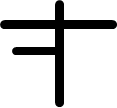
\includegraphics[width=1.1\@tempdima,height=1.3\@tempdimb]{images/plusminus.png}\,
}

% Minusplus (neu)
\newcommand*\leibvdash{%
   	\settowidth{\@tempdima}{$m$}% 
   	\settoheight{\@tempdimb}{$b$}% 
	\protect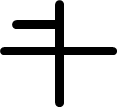
\includegraphics[width=1.1\@tempdima,height=1.3\@tempdimb]{images/minusplus.png}\,
}

% Groesser
\newcommand*\ggroesser{%
   	\settowidth{\@tempdima}{$m$}% 
   	\settoheight{\@tempdimb}{$b$}% 
	\protect
\includegraphics[width=0.55\@tempdima,height=1.3\@tempdimb]{images/groesser.png}
}
\DeclareRobustCommand\groesser{%
	\settoheight{\@tempdimb}{$b$}% 
	$\raisebox{-0.55\@tempdimb}[0pt][8pt]{\ggroesser}\!$
}

% Kleiner
\newcommand*\kkleiner{%
   	\settowidth{\@tempdima}{$m$}% 
   	\settoheight{\@tempdimb}{$b$}% 
	\protect
\includegraphics[width=0.55\@tempdima,height=1.3\@tempdimb]{images/kleiner.png}
}
\DeclareRobustCommand\kleiner{%
	\settoheight{\@tempdimb}{$b$}% 
	$\raisebox{-0.55\@tempdimb}[0pt][8pt]{\kkleiner}\!$
}

% Alchemistisches Zeichen Doppelsigma
%\newcommand*\dsig{%
   	%\settowidth{\@tempdima}{$v$}% 
   	%\settoheight{\@tempdimb}{$v$}% 
	%\protect
\includegraphics[width=1.6\@tempdima,height=1.1\@tempdimb]{images/dsig.pdf}
\newcommand*\dsig{%
   	\settowidth{\@tempdima}{$v$}% 
   	\settoheight{\@tempdimb}{$v$}% 
	\protect
\includegraphics[width=1.7\@tempdima,height=1.15\@tempdimb]{images/dsig.png}
}
\makeatother 

% K.Zeitz: Ende neue Definitionen


\def\largerthan{$\raisebox{0.8pt}{$\urcorner$} \hspace{-5.5pt}|\hspace{3pt}$} %fuer groesser als
\newcommand{\GWLypsilon}{\raisebox{2pt}{\text{\tiny{o}}}\hspace{-1pt}\upsilon}

 
% Seitenlayout
\usepackage[paperwidth=190mm, paperheight=246mm, textwidth=135mm, textheight=178mm,
  hmarginratio=2:3, tmargin=21mm, bmargin=47mm, twoside, includehead, headsep=5mm]{geometry}
\flushbottom

%Kolumnentitel: linke Druckseite zentriert Part-Titel, rechte Seite aktuelle chapter oder section
\automark[chapter]{part}
\newmarks\numbermark
\renewcommand*{\chaptermark}[1]{%
  \marks\numbermark{\chaptermarkformat}%
  \markright{#1}%
}      
\makeatletter% 
  \renewcommand*{\sectionmark}[1]{%
  \begingroup
  \@temptokena\expandafter{\sectionmarkformat}%
  \marks\numbermark{\the\@temptokena}%
  \endgroup
  \markright{#1}%
  }
\makeatother
        
\clearscrheadfoot
\ohead[\pagemark]{\pagemark}
\ihead[{\botmarks\numbermark}]{\botmarks\numbermark}
\chead[\headmark]{\headmark}   
%CH: Keine Partnummern in den automatischen Kolumnentiteln
\renewcommand*{\partmarkformat}{}
%Formatierug der Kapitelnummer im header
\renewcommand*{\chaptermarkformat}{N.\ \arabic{chapter}}
%Formatierung der Sectionnummer im header
\newcommand{\notsotiny}{\fontsize{7pt}{8pt}\selectfont}
\renewcommand*{\sectionmarkformat}{% 
  N.\ \arabic{chapter}\raisebox{-0.5ex}{\notsotiny\arabic{section}}}
\setkomafont{pagehead}{\normalfont\small}
%\setkomafont{pagehead}{\notsotiny}
\setkomafont{pagenumber}{\normalfont\normalsize}
\setheadsepline{0.4pt}
\pagestyle{scrheadings}


%erste Seiten
%erste Seite eines neuen Teils
\renewcommand*{\partpagestyle}{empty}
\renewcommand*{\partformat}{}
\setkomafont{part}{\normalfont\MakeUppercase}
%\renewcommand*{\partheadstartvskip}{\vspace*{-9.5ex}}
\renewcommand*{\partheadstartvskip}{\vspace*{-6ex}}
%CH: Part-Ueberschriften auf der neuen leeren Seite linksbuendig ausgeben
\renewcommand*{\raggedpart}{\raggedright}
 
%erste Seite eines neuen Kapitels
%Punkt immer hinter Kapitelnummer und weitere Formatspezifikationen
\renewcommand{\thechapter}{\arabic{chapter}.}
\renewcommand*{\chapterformat}{%
  \chapappifchapterprefix{\ }\thechapter\enskip}
\renewcommand*{\chapterpagestyle}{scrheadings}
\renewcommand*{\chapterheadstartvskip}{\vspace*{-5mm}}
%schnoepf2001\setkomafont{chapter}{\normalfont\normalsize\uppercase}
\setkomafont{chapter}{\normalfont\normalsize}
%\addtokomafont{chapter}{\scshape}

\renewcommand*{\chapterheadendvskip}{\vspace*{0mm}}

%erste Seite des ersten Kapitels im Part (keine Kolumnenzeile)
\newpagestyle{firstchapter}{(0pt,0pt){}{}{}(0pt,0pt)}{{}{}{}}

% section-Formatierung: Schriftgroesse, Nummerierung mit tiefgestellten Zahlen
% und weitere Formatspezifikationen
%schnoepf2001\setkomafont{section}{\normalfont\normalsize\uppercase}
\setkomafont{section}{\normalfont\normalsize}
%\addtokomafont{section}{\scshape}
\renewcommand{\thesection}{\arabic{chapter}\protect\raisebox{-0.5ex}{\notsotiny\arabic{section}}\autodot}
\renewcommand*{\othersectionlevelsformat}[1]{%
  \csname the#1\endcsname\enskip}


%Haupttext
%Zeilendurchschuss
\renewcommand{\baselinestretch}{1.1}
%Absatzueinrckung
\parindent=7.5mm
%Seitenumbruch
\frenchspacing     
%\clubpenalty=9999 % keine Schusterjungen
%\widowpenalty=9999 % keine Hurenkinder
\tolerance=1750 % Zeilenumbruch-Toleranz (ca. 500--3000)
%headerelemente
\newcommand{\link}[1]{\ref{#1}}
\renewcommand{\title}[2][]{\cite{#1}\textit{#2}}

%Zeilenzaehler
\lineation{page}
\linenummargin{outer}
\setcounter{firstlinenum}{5}
\setcounter{linenumincrement}{5}
%5 rechtsbuendig
\makeatletter
  \renewcommand{\rightlinenum}{\ifbypage@\ifnum\line@num<10\kern.5em\fi\else 
  \ifnum\line@num<10\kern1em\else\ifnum\line@num<100 \kern.5em\fi\fi\fi\kern.5em\numlabfont\the\line@num 
  \ifnum\subline@num>0:\the\subline@num\fi} 
\makeatother

\renewcommand{\footfudgefiddle}{71}
%Afootnotes = Marginalien written by GWL
\footnormal{A}
\setlength{\skip\Afootins}{8mm plus 3mm minus 3mm} %amount of whitespace between text and footnotes
\renewcommand{\Afootnoterule}{\noindent\rule{18mm}{0.4pt}\vspace*{3.0mm}}
\newcommand{\Afootnotefontsetup}{\normalsize}
\makeatletter
  \renewcommand{\ledsetnormalparstuff}{%
    \normal@pars
    \parindent \z@ \parfillskip \z@ \@plus 1fil \vspace{1pt}}
\makeatother
\makeatletter
\renewcommand*{\Afootfmt}[3]{%
	\normalsize
	\setstretch{1.3}
	\ledsetnormalparstuff
	\mbox{{\notenumfont\printlines#1|}\enspace
	{\select@lemmafont#1|#2}}\enskip#3\strut\par%
}
\makeatother
\count\Afootins=1500

%Kritische Apparate
%Bfootnotes = Varianten, Textgenese
\setlength{\skip\Bfootins}{5mm plus 2mm minus 2mm}
\renewcommand{\Bfootnoterule}{\rule{0mm}{0pt}\vspace*{1mm}}
\footparagraph{B}
\interparanoteglue{7.5mm plus1.9mm minus1.9mm}
\makeatletter
  \renewcommand*{\Bfootfmt}[3]{%
  \noindent
  \mbox{{\notenumfont\printlines#1|}\enspace
  {\select@lemmafont#1|#2}}\enskip#3\strut\par}
\makeatother
\count\Bfootins=1500
%
%Cfootnotes, Kommentare der Editoren
\setlength{\skip\Cfootins}{1mm plus 0mm} %KZeitz
\renewcommand{\Cfootnoterule}{\rule{\textwidth}{0.4pt}\vspace*{1mm}} 
\footparagraph{C}
\interparanoteglue{7.5mm plus 1.9mm minus 1.9mm}
\makeatletter
  \renewcommand*{\Cfootfmt}[3]{%
  \noindent
  \mbox{{\notenumfont\printlines#1|}\enspace
  {\select@lemmafont#1|#2}:}\enskip#3\strut\par}
\makeatother
\count\Cfootins=1500
%commands for bibliographical data in Cfootnotes
\newcommand{\biblio}[3]{\textsc{#1}, \textit{#2}, S. #3.}
\newcommand{\biblioplus}[5]{\textsc{#1}, \textit{#2}, S. #3, (\textit{#4}, S. #5).}
%\newcommand{\biblionote}[2]{\Cfootnote{\textsc{#1}, \textit{#2},\ }} requires \edtext, impractical
%more space for crit apparatus
\renewcommand{\footfudgefiddle}{500}

% Ausgabe einer Zeilenreferenz mit 'f', sofern sich die Fussnote auf genau zwei 
% aufeinanderfolgende Zeilen bezieht.
% K. Zeitz: Zusätzliche Ergänzung: Möglichkeit, die Zeilenreferenz in der Fußnote mit Hilfe des unten
% definierten Befehls \killnumber ganz zu unterdrücken.
\makeatletter
\def\printlines#1|#2|#3|#4|#5|#6|#7|{%					
	\begingroup
		\setprintlines{#1}{#2}{#3}{#4}{#5}{#6}%
			\ifnum #1=#4
				\ifnum #2<#5
					\newcount\endlinenumber
					\endlinenumber = #5
					\advance\endlinenumber by -1
					\ifnum #2<\endlinenumber 
						#2\endashchar#5\else #2f\fullstop
					\fi       
				\fi 
				\ifnum#2=-1 % K. Zeitz: Neu
					\symplinenum  \hspace*{-1.4em} % K. Zeitz: Neu 
				\else % K. Zeitz: Neu
					\ifnum #2=#5 #2 \fi
				\fi % K. Zeitz: Neu
			\fi
			\ifnum #1<#4							
			\ifl@d@pnum 
				#2\endashchar S\fullstop\ #4\fullstop
			\fi
			#5
		\fi
	\endgroup%
}
\makeatother

% K.Zeitz: Unterdrückung der Referenz auf die Zeilennummer in Fußnoten.
% Dazu den nachfolgend definierten Befehl \killnumber wie folgt einfügen:
%		\edtext{...}{\lemma{...}\killnumber\Afootnote{...}}
% Analog für \Bfootnote und \Cfootnote
\newcommand{\killnumber}{\linenum{|-1|||-1||}} 
 
%Ueberschriften, Inhaltsverzeichnis, Indizes
%titlepages set by hand / publisher
%Inhaltsverzeichnis
%Name des Inhaltsverzeichnisses      
\addto\captionslatin{%
\def\contentsname{}}
%\maxtocdepth{section}
%\maxtocdepth{part}

% Ein durch \edlabel{LH-Nummer_n} … \edlabel{LH-Nummer_n+1} bestimmter Referenzbereich lässt sich mit dem Befehl \refpassage{LH-Nummer_n}{LH-Nummer_n+1} innerhalb von footnotes als Querverweis (Seite.Zeile-Seite.Zeile) anführen. H.S.%
\newcommand{\refpassage}[2]{%
\xpageref{#1}\fullstop\xlineref{#1}%
\ifnum\xpageref{#1}=\xpageref{#2}
\ifnum\xlineref{#1}=\xlineref{#2}
\else
\endashchar\xlineref{#2}%
\fi
\else
\endashchar\xpageref{#2}\fullstop\xlineref{#2}%
\fi
}
%%Textausrichtung bei fester Spaltenbreite %H.S.
%\usepackage{tabularx}
%\newcolumntype{L}[1]{>{\raggedright\arraybackslash}p{#1}} % linksbündig mit Breitenangabe
%\newcolumntype{C}[1]{>{\centering\arraybackslash}p{#1}} % zentriert mit Breitenangabe
%\newcolumntype{R}[1]{>{\raggedleft\arraybackslash}p{#1}} % rechtsbündig mit Breitenangabe
%
%


%Aufnahme der Chapter- und Sectiontitel ins Inhaltsverzeichnis unterdruecken
\newcommand*\OrigChapter[2][]{}
\let\OrigChapter\chapter
\renewcommand*{\chapter}[2][]{%
  \settocdepth{part}\OrigChapter[#1]{#2}%
  \settocdepth{section}%
  }
\newcommand*\OrigSection[2][]{}
  \let\OrigSection\section
\renewcommand*{\section}[2][]{%
  \settocdepth{part}\OrigSection[#1]{#2} %
  \settocdepth{section}%
  }

%Aufnahme der parts ins Inhaltsverzeichnis verhindern
%\newcommand*\OrigPart[2][]{}
 % \let\OrigPart\apart
%\renewcommand*{\apart}[2][]{%
 % \settocdepth{apart}\OrigPart[#1]{#2} %
 % \settocdepth{section}%
  %}
%\makeatletter
%\let\settocdepth\relax
%\newcommand{\settocdepth}[-1]{%
  %\addtocontents{toc}{\protect\setcounter{tocdepth}{#1}}}
%\makeatother
%Format des Inhaltsverzeichnisses
\tocloftpagestyle{empty}
%Kopfzeile
\makeatletter
  \renewcommand{\cftmarktoc}{%
%  \@mkboth{\scshape Inhaltsssverzeichnis}{\scshape Inhaltsverzeichnis}}
  \@mkboth{\scriptsize\uppercase{Inhaltsverzeichnis}}{\scriptsize\uppercase{Inhaltsverzeichnis}}}
  \renewcommand*{\l@part}{\@dottedtocline{-1}{0mm}{0mm}}
 % \renewcommand*{\l@chapter}{\@dottedtocline{0}{2mm}{6mm}}
  \renewcommand*{\l@chapter}{\@dottedtocline{0}{2mm}{6mm}}
 %   \setlength{\cftsecnumwidth}{35mm}
  \renewcommand*{\l@section}{\@dottedtocline{1}{8mm}{7mm}}
  \renewcommand{\@pnumwidth}{9mm}
\renewcommand{\@tocrmarg}{9.5mm}
  \renewcommand{\@dotsep}{4.5}
\makeatother



%Bibliografie
%Keine Ueberschrift fuer die Bibliografie
\addto\captionslatin{\def\bibname{\ \vspace{1.6ex}}}

% Werke in der Bibliographie werden mit '1., 2.' durchnummeriert
%\cite-Befehl gibt nichts aus
\makeatletter
  \renewcommand{\@biblabel}[1]{#1.}
  \renewcommand*{\@cite}[2]{{#1\if@tempswa , #2\fi}}
\makeatother
        
%\cite-Befehl gibt nichts aus
\makeatletter
  \def\@citex[#1]#2{\leavevmode
  \let\@citea\@empty
  \@cite{\@for\@citeb:=#2\do
  {\@citea\def\@citea{,\penalty\@m\ }%
  \edef\@citeb{\expandafter\@firstofone\@citeb\@empty}%
  \if@filesw\immediate\write\@auxout{\string\citation{\@citeb}}\fi
  }}{#1}}
\makeatother
       
%Indices
\makeindex{Namensregister}
\makeindex{Sachverzeichnis}
\makeindex{Ortsregister}
%Index zweispaltig, mit 'Praeambel'
\makeatletter

 % \renewcommand{\see}[2]{{\em s.\/a.\/} #1}
   \renewcommand{\see}[2]{\newline{\em s.\/a.\/} #1}
  \renewcommand\printindex[2]{
  \clearpage{\pagestyle{empty}\cleardoublepage}
  \setchapterpreamble{\index@preamble}
  \addchap*{\hfill #2\hfill}
  \thispagestyle{empty}
  \clearscrheadings
  \chead{\sc{#2}}
  \ohead[\pagemark]{\pagemark}
  \begin{multicols}{2}\setlength{\columnseprule}{0.4pt}
  \footnotesize\raggedright
  \@input{#1.ind}
  \end{multicols}}
  \renewcommand*\@idxitem{\par\hangindent 11\p@}
 % \renewcommand*\subitem{\@idxitem \hspace*{11\p@}}
  \renewcommand*\subitem{\@idxitem \par\hangindent 22\p@ \hspace*{11\p@}}
  %\renewcommand*\@idxsubitem{\@idxsubitem \hspace*{11\p@}}
\makeatother
\newcommand\efrac[2]{\genfrac{}{}{0pt}{}{#1}{#2}} %KZeitz \efrac produziert einen Bruch ohne Bruchstrich

%neuer Vorspann
\begin{document}




%Titelseite
        \begin{titlepage}
        \begin{center}
        \pagenumbering{Roman}
        {\huge GOTTFRIED WILHELM}\\
        \vspace*{7.5mm}
        {\Huge LEIBNIZ}\\
        \vspace*{10.5mm}
        {\Large SAEMTLICHE\\
        SCHRIFTEN UND BRIEFE}\\
        \vspace*{13mm}
        {\large HERAUSGEGEBEN\\
        VON DER}\\
        \vspace*{6.5mm}
        {\Large BERLIN-BRANDENBURGISCHEN\\
        AKADEMIE DER WISSENSCHAFTEN}\\
        {\large UND DER}\\
        {\Large AKADEMIE DER WISSENSCHAFTEN\\
        IN GOETTINGEN\\
        \vspace*{16mm}
        ACHTE REIHE}\\
        {\large NATURWISSENSCHAFTLICHE, TECHNISCHE UND MEDIZINISCHE SCHRIFTEN}\\
        \vspace*{5.5mm}
        {\Large ZWEITER BAND}\\
        Korrekturvorlage\\
        \vspace*{6mm}
        \large{Dies ist eine Korrekturvorlage. Umfang und Bearbeitungszustand der Texte entsprechen nicht dem fertigen Band.}\\ %KZeitz
        \end{center}
        \end{titlepage}
%Titelseite_Ende

\pagenumbering{Roman}
%\beginnumbering

%CH \part und \addpart* geaendert, damit Ueberschrift keine Nummer und nicht ins Inhaltsverzeichnis
\clearpage{\pagestyle{empty}\cleardoublepage}
\addpart[\large\uppercase{Inhaltsverzeichnis}]{\large\protect\textso{INHALTSVERZEICHNIS}}

\clearpage{\pagestyle{empty}\cleardoublepage}
   \tableofcontents



\clearpage{\pagestyle{empty}\cleardoublepage}
\addtocontents{toc}{\vspace{5mm}}
\addpart[\large\uppercase{Vorwort}]{\large\protect\textso{VORWORT}}
\clearpage{\pagestyle{empty}\cleardoublepage}
\markleft{\scriptsize\uppercase{Vorwort}}
%   \selectlanguage{german}
\thispagestyle{empty}
{\vrule height 0mm depth 30mm width 0mm}
\vspace*{2em}
\par\noindent 
Die Reihe VIII der Leibniz-Edition ist ein durch das Akademienprogramm gefördertes Langzeitvorhaben der Berlin-Brandenburgischen Akademie der Wissenschaften. Nach Erkenntnissen der von 2013 bis 2014 durchgeführten Nachkatalogisierung wird die Reihe der naturwissenschaftlichen, medizinischen und technischen Schriften in einem Umfang von zwölf Bänden erscheinen (2 Bde mit Schriften aus der Mainzer und Pariser Zeit zu allen drei Teilen der Reihe, 6 Bde Naturwissenschaft, 2 Bde Medizin, 2 Bde Technik). 
\newline\indent
Gedankt sei den öffentlichen Geldgebern für die Finanzierung des Vorhabens, dem Bundesministerium für Bildung und Forschung sowie der Senatsverwaltung für Wirtschaft, Technologie und Forschung des Landes Berlin. Arbeitsgrundlage für die Berliner Leibniz-Edition sind die Digitalisate der in Reihe VIII zu edierenden Handschriften. Sie sind dank der umfassenden Finanzierung seitens der Deutschen Forschungsgemeinschaft in hochauflösender Qualität angefertigt worden und werden freundlicherweise von der Gottfried Wilhelm Leibniz Bibliothek zur Verfügung gestellt. Dank der großzügigen Finanzierung sowohl durch die Alfried Krupp von Bohlen und Halbach-Stiftung als auch durch die Stiftung der Versicherungsgruppe Hannover sind die Digitalisate online zugänglich (http://ritter.bbaw.de). \par
Der Niedersächsischen Landesbibliothek ist des Weiteren für ihre Unterstützung zu danken, insbesondere in Person ihrer Mitarbeiterin Anja Fleck, die für die Berliner Arbeitsstelle Reproduktionen anfertigen ließ sowie die Autopsie von Handschriften vornahm. Durch die Leibniz-Forschungsstelle Hannover hat die Arbeit an VIII,2 vielfach Unterstützung erfahren: Siegmund Probst verdanken wir zahlreiche wertvolle Hinweise auf Handschriften und auf von Leibniz benutzte Literatur sowie zu Fragen der Datierung und der mathematischen Notation; bei Charlotte Wahl bedanken wir uns für die Scans  von Leibnitiana, die sie uns aus dem Stadtarchiv Göttingen beschaffte; Achim Trunk teilte dankenswerterweise Erkenntnisse mit uns, die er über die komplexen kombinierten Vorzeichen, die Leibniz in der zweiten Hälfte 1674 verwendete, gewonnen hatte. Die Arbeiten am Band haben auf unterschiedliche Weise auch durch die Arbeitsstellen in Potsdam und Münster Unterstützung erfahren. Des Weiteren danken wir Annie Bitbol-Hespériès für alternative Lesarten von Stellen in Descartes' Manuskripten und Kees Verduin
%Dr. Kees Verduin (Universität Leiden)
für seine Nachforschungen zu dem von Leibniz verwendeten und von Christiaan Huygens stammenden Exemplar der \textit{Mechanica} von John Wallis. Martin Frank danken wir für seine bibliographische Recherche zu Literatur, die Leibniz zitiert.\par
Die setzerischen Herausforderungen bei der Fertigstellung des vorliegenden Bandes hat Katharina Zeitz gemeistert. Ihrem unermüdlichen Einsatz durch alle Phasen der Manuskriptgestaltung und -erstellung ist es zu verdanken, dass zahlreiche Probleme des Layouts und der Zeichendarstellung in \LaTeX\ gelöst werden konnten. Für die gute Zusammenarbeit danken wir Gertrud Grünkorn und Maik Bierwirth vom De Gruyter Verlag.
\par
\vspace*{2em}
Berlin, im Juli 2016\hspace{65mm}Harald Siebert






\clearpage{\pagestyle{empty}\cleardoublepage}
\addtocontents{toc}{\vspace{5mm}}
\addpart[\large\uppercase{Einleitung}]{\large\protect\textso{EINLEITUNG}}
\clearpage{\pagestyle{empty}\cleardoublepage}
\markleft{\scriptsize\uppercase{Einleitung}}
%   %\thispagestyle{empty}
\selectlanguage{german}
%{\vrule height 0mm depth 30mm width 0mm}
%\newpage
%\noindent
\thispagestyle{empty}
{\vrule height 0mm depth 30mm width 0mm}
%\par
%\noindent
\vspace*{2em}
\par\noindent Der vorliegende zweite Band der naturwissenschaftlichen, medizinischen und technischen Schriften vereint 99 Stücke aus allen drei Teilbereichen der 2001 gegründeten Reihe VIII der Leibniz-Edition. Fast alle in diesem Band edierten Texte sind in den Jahren, die Leibniz in Paris verbrachte (1672 bis 1676), entstanden. Keine der hier herausgegebenen Schriften war zu seinen Lebzeiten erschienen; der Text von insgesamt 14 Stücken wurde teilweise oder ganz im Zeitraum von 1849 bis 2001 abgedruckt (N. 6, N. 11, N. 12, N.~$36_2$, N. 50, N. 54, N. 55, N. 58, N. 69, N. 70, N. 76, N. 81, N. 82, N. 98). Dagegen werden 85 Stücke in diesem zweiten Band erstmals veröffentlicht und können damit erst jetzt eine Leserschaft finden. Bis auf wenige Ausnahmen stehen alle Handschriften, die Gegenstand der Reihe VIII sind, in hochauflösenden Digitalisaten online zur Verfügung (http://ritter.bbaw.de). Dies gilt auch für die Stücke dieses Bandes bis auf diejenigen, die Marginalienexemplare (N. 3, N. 13, N. 44, N. 46, N. 47), einen Druck (N. 81) oder erst jüngst entdeckte Handschriften aus Hannover (N. 51) oder Göttingen (N. 66) zur Vorlage haben.
\par\vspace{6.0ex}
\noindent
\noindent\uppercase{Themen des Bandes}
\par
\vspace{1.0ex}
\noindent
Der zweite Band bildet eine chronologische Einheit mit dem im Jahre 2009 erschienenen ersten Band der Reihe: Beide Bände decken die Pariser Jahre ab, in denen sich Leibniz hoch produktiv und vielfältig mit unterschiedlichen Themen auf verschiedenen Gebieten beschäftigte, neue Felder für sich entdeckte, sich mit Zeitgenossen und dem Forschungsstand seiner Zeit auseinandersetzte. Wie im ersten Band der Pariser Jahre folgt die thematische Einteilung seiner Schriften der Klassifikation, die Leibniz selbst im März 1673 in seinen \textit{Observata Philosophica} (VIII,1 N. 1) gegeben hat. Daher entspricht die Gliederung des Bandes nicht unserem heutigen Verständnis von Fachgebieten und -grenzen.\par 
\newpage
Der erste Band der Schriften aus der Pariser Zeit enthält Stücke zur Nautik (Nautica), Optik (Optica), Pneumatik (Pneumatica) und Technik (Technica). Der zweite Band verschafft der Rubrik Technica einen Zuwachs von 17 Stücken (N. 83 - N. 99) in Form von Nachträgen zum ersten Band. Rubriken, die in VIII,2 neu hinzukommen und sich auf Leibnizens Einteilung von 1673 stützen, sind Astronomica (N. 1, N. 2), Magnetica (N. 3 - N. 6), Mechanica (N. 7 - N. 52), Meteorologica (N. 53, N. 54), Physica (N. 55 - N. 57), Anatomica (N. 58), Botanica (N. 59, N. 60), Chymica (N. 61 - N. 65), Medica (N. 66 - N. 77) und Miscellanea (N. 78 - N. 81).\par
Schriften zur Mechanik haben den weitaus größten Anteil im Band, sowohl was die Anzahl der Stücke (46) als auch den Seitenumfang (374 Seiten) angeht. Leibniz beschäftigt sich hier mit verschiedenen Teilgebieten, die er in seiner Klassifikation von 1673 nicht eigens berücksichtigt. Sie bilden in dem vorliegenden Band folgende Unterrubriken zur Mechanik: Allgemeines, Bewegung, Festigkeit, Kraft, Reibung, spezielle Probleme und Stoß. Innerhalb der Mechanik sind es die Stücke zur Reibung (123 Seiten), die mit Abstand den größten Umfang haben, gefolgt von Stücken zu allgemeinen Problemen (80 Seiten); dagegen nehmen die weiteren Unterrubriken zur Mechanik jeweils deutlich weniger Raum ein, variieren aber in ihrem Umfang: Stoß (42 Seiten), Kraft (38 Seiten), Festigkeit (35 Seiten), spezielle Probleme (33 Seiten), Bewegung (23 Seiten). \par
Mit den naturwissenschaftlichen (Astronomica, Magnetica, Mechanica, Physica, Chymica), medizinischen (Anatomica, Botanica, Medica) und technischen (Technica) Schriften, die hiermit herausgegeben werden, vereint der aktuelle Band erstmals alle drei Teilbereiche der Reihe VIII. In dieser Hinsicht wird VIII,2 ein Unikum bleiben, da geplant ist, in allen weiteren Bänden der Reihe nur Schriften jeweils eines Teilbereichs zu edieren. 
\par\vspace{6.0ex}
\noindent
\noindent\uppercase{Stücke, Sprachen, Textarten}
\par\vspace{1.0ex}
\noindent
Von den gezählten 99 Stücken des Bandes zerfallen sieben in insgesamt 27 Unterstücke. Diese 119 Stücke und Unterstücke unterscheiden sich in Textart und Sprache. Auf Lateinisch sind 78 Stücke und Unterstücke geschrieben, auf Französisch 36, auf Deutsch vier (ein weiteres Stück besteht nur aus Zeichnungen); in 18 Fällen verwendet Leibniz zusätzlich noch weitere Sprachen (neben Lateinisch, Französisch und Deutsch sind dies Italienisch und Englisch). Eigentümlichkeiten in der Orthographie der von Leibniz benutzten französischen Sprache werden im Rahmen der Editionsrichtlinien beibehalten (z.B. \textit{servic} für \textit{service}, \textit{resistence} für \textit{résistance}).\par
\newpage
Das Gros der Stücke besteht aus 42 Aufzeichnungen (N. 4, N. 5, N. 11, N. 14, N.~$17_1$, N. $17_2$, N. 18, N. 20, N. 22 - N. 26, N. 33, N. $34_5$, N. 39, N. 42, N. 43, N. 49, N.~51, N. 52, N. 60, N. 63, N. 64, N. 69, N. 71, N. 72, N. 75, N. 83 - N. 87, N. 90, N.~96, N. $97_1$ - N. $97_4$, N. 99). Dabei handelt es sich um ausführlichere Notizen, die sich Leibniz von eigenen und fremden Gedanken, Erfahrungen, Beobachtungen, Berichten macht, oder um Listen, Rechnungen oder Zeichnungen, die er erstellt; darunter finden sich auch drei Gesprächsnotizen (N. 65, N. 77, N. 88). Von diesen 42 Aufzeichnungen sind 26 auf Lateinisch, 14 auf Französisch und zwei auf Deutsch verfasst; Nebensprachen sind Lateinisch in zwei französischen Aufzeichnungen (N. 77, N. 99), Deutsch (N. 84, N. 85) in zwei lateinischen und Italienisch in einer lateinischen (N. 22). Die meisten Aufzeichnungen stammen aus der Rubrik Technik (11), mit deutlichem Abstand gefolgt von zwei Unterrubriken der Mechanik, Festigkeit (6) und Bewegung (4), sowie der Medizin (5). \par
Als zweithäufigste Textart enthält der Band 31 Konzepte (N. 9, N. 10, N. 12, N. 15, N. 19, N. 21, N. 27, N. $28_5$, N. $28_6$, N. 29, N. 30, N. $31_2$, N. $31_3$, N. 32, N. $34_1$ - N. $34_4$, N.~35, N. 41, N. $45_1$ - N. $45_3$, N. 62, N. 78, N. 89, N. 91 - N. 94, N. $97_1$), d.h. längere Texte, teils mit ausformulierten Überschriften, die den Charakter von Entwürfen haben und zur weiteren Ausarbeitung, für Vorträge, zur Weitergabe oder zur Veröffentlichung bestimmt gewesen sein dürften. 26 Konzepte sind auf Lateinisch, die übrigen fünf auf Französisch geschrieben; Nebensprachen sind Französisch (N. $34_2$, N. 35, N. $45_1$, N. 78), Lateinisch (N. $34_1$) und Italienisch zusammen mit Deutsch (N. 78). Die meisten Konzepte stammen aus der Unterrubrik Reibung (9), gefolgt von der Rubrik Technik (6) und den weiteren Unterrubriken Kraft (4) und Spezielle Probleme (4).\par
Die dritthäufigste Textart im Band stellen die 20 Auszüge dar, d.h. Exzerpte oder Paraphrasen, die Leibniz aus gedruckten, handschriftlichen oder verschollenen Vorlagen erstellt und kommentiert hat (oder wie in N. $31_1$, N. 66 unkommentiert lässt). 16 Auszüge sind auf Lateinisch geschrieben, die übrigen vier auf Französisch; Nebensprachen sind Französisch (N. 7, N. 56), Lateinisch (N. 50), Deutsch (N. 68) und Englisch (N. 2). Die Themen der exzerpierten Literatur sind breit gestreut: Jeweils vier Auszüge gehören zur Mechanik (N. 7, N. 8, N. $31_1$, N. 50) und Medizin (N. 66, N. 68, N. 74, N. 76), drei zur Physik (N. 55 - N. 57), jeweils zwei zur Astronomie (N. 1, N. 2), Meteorologie (N. 53, N. 54) und Technik (N. 82, 98) sowie jeweils ein Auszug zur Anatomie (N. 58), Botanik (N. 59) und zum Magnetismus (N. 6). Zeichnungen, die ohne Stellennachweise in den edierten Auszügen wiedergegeben werden, sind von Leibniz selbst angefertigt, insofern dies anhand einer erhaltenen Vorlage überprüfbar gewesen ist. Nicht erhalten sind die Vorlagen derjenigen Auszüge, die Leibniz von Manuskripten aus dem verschollenen Nachlass René Descartes' (N. 6, N. 54, N. 58, N. 76, N. 82) und von einem verlorenen Manuskript Ole R{\o}mers (N. 98) anfertigt; die einzige Überlieferung bietet Leibniz auch für das Manuskript eines gewissen Herrn Acar (N. 74) und für ein weiteres von Claude Perrault (N. 57).\par
Eine vierte Gruppe an Texten bilden die zwölf Reinschriften, davon neun mit Verbesserungen (N. $28_2$ - N. $28_4$, N. $28_7$, N. 37, N. 38, N. $45_4$, N. 48, N. 70), zwei mit Verbesserungen und  Ergänzungen (N. $36_1$, N. $36_2$) und eine einzige von Schreiberhand (N. $28_1$). Die Reinschriften stammen bis auf eine Ausnahme (N. 70: Medica) sämtlich aus der Rubrik Mechanik, und zwar aus den Unterrubriken Kraft (5), Reibung (4), spezielle Probleme (1) und Stoß (1).\par
Eine kleinere Gruppe stellen die sieben Notizen (N. 16, N. 40, N. 61, N. 79, N. 80, N. 88, N. 95) dar, die den Aufzeichnungen als Textart nicht unähnlich sind, nur dass sie kürzer ausfallen und eher fragmentarischen Charakter haben. Drei dieser Notizen sind auf Lateinisch, eine auf Französisch, eine auf Deutsch geschrieben; eine weitere (N. 79), die größtenteils nicht von Leibniz stammt, ist mehrsprachig (Lateinisch, Italienisch, Deutsch, Französisch). Die nächstkleinere Gruppe an Stücken besteht aus sechs Anstreichungen mit Anmerkungen in Handexemplaren (N. 3, N. 13, N. 44, N. 46, N. 47, N. 67) lateinischer und französischer Bücher. Hier gibt die Edition Text und Zeichnungen des von Leibniz gelesenen Buches zu denjenigen Stellen wieder, die er markiert oder kommentiert hat. Informationen über seine Anstreichungen und den Inhalt seiner Anmerkungen liefert (wenn nicht anders vermerkt) der Marginalienapparat zur jeweiligen Seite.\par
Einen Einzelfall unter den im Band auftretenden Textarten stellt eine Abschrift (N.~73) dar, die Leibniz von einer Vorlage auf Französisch macht, die unbekannt ist. Da es dadurch keine Möglichkeit der Überprüfung gibt, könnte es sich hierbei auch um einen Auszug handeln.\par
\par\vspace{6.0ex}
\noindent
\noindent\uppercase{Datierung, inhaltliche Schwerpunkte und zeitlicher Verlauf}
\par\vspace{1.0ex}
\noindent
Die textkritische Ausgabe dokumentiert alle Änderungen und Ergänzungen und liefert die Marginalien, mit denen Leibniz den Inhalt seiner Schriften nachträglich kommentiert hat. Wann die Genese eines Textes jeweils ihren Abschluss fand und den heute erhaltenen Textbestand erreichte, lässt sich selten mit Sicherheit sagen. Nachträgliche Überarbeitungen sind nicht auszuschließen; zahlreiche Textschichten, wie sie der Variantenapparat dokumentiert, können, müssen aber kein Hinweis darauf sein, dass Leibniz in wiederholten Anläufen an einem Stück gearbeitet hat. Spätere Zusätze lassen sich selten wie in N. $36_2$ datieren: Dieses Stück zur Reibung ist laut Leibniz im Winter 1675 entstanden, während der Zusatz aus der Zeit nach Paris stammen muss. In zwei Fällen liefert uns Leibniz explizit das Datum einer späteren Überarbeitung: Den eigenhändig datierten Entwurf zum Perpetuum mobile (N. 92) aus dem Jahr 1674 nimmt er sich im Mai 1678 nochmals vor und formuliert einen Zusatz; eine spätere Ergänzung genau zu derselben Zeit erfährt ein weiteres Stück (N. 96) aus der Rubrik Technik: Leibniz korrigiert hier drei Jahre später Berechnungen, die er 1675 angestellt hat. Mit diesen drei Stücken zusammen sind im Ganzen 16 des Bandes eigenhändig von Leibniz datiert (N.~10, N. 11, N. 32, N. 34, N. $36_2$, N. 51, N. 52, N. 64, N. 65, N. 75, N. 76, N. 79, N.~92, N.~96, N. $97_1$, N. 98); im ersten Band der Reihe trifft dies nur auf insgesamt sechs Stücke zu.\par
Wie bereits der erste Band der Pariser Jahre enthält auch der zweite Schriften, die noch in der Mainzer Zeit entstanden sind (N. 39, N. 55, N. 66, N. 67, N. 69, N. 70, N.~71, N. 83). Die zwei ältesten (N. 39, N. 66) dieser insgesamt acht Stücke sind zugleich diejenigen des Bandes, die am ungenauesten datierbar sind: Beide haben ihre untere Datierungsgrenze im Jahr 1668, und ihre mögliche Entstehung erstreckt sich über eine Spanne von 47 bzw. 43 Monaten. Mit Ausnahme von vier weiteren Stücken (N. 47, N.~55, N. 73, N. 74) ist es bei allen übrigen gelungen, die jeweilige Entstehungszeit auf einen Zeitraum von maximal 13 Monaten einzugrenzen.\par 
Die 93 Stücke des Bandes, die mit dieser Genauigkeit datiert sind, können Aufschluss darüber geben, wie Leibniz sich im Verlauf seiner Pariser Zeit mit den verschiedenen Themen beschäftigte, die Gegenstand der in diesem Band veröffentlichten Schriften sind. In den acht noch in Mainz (von 1668 bis Februar 1672) entstandenen Stücken setzt sich Leibniz mit medizinischen Fragen (N. 67, N. 68, N. 69, N. 70, N. 71), mit Mechanik (N. 39) und mit der technischen Realisierung eines Perpetuum mobile auseinander (N. 83); daneben verfasst er sehr umfangreiche Exzerpte zur Physik (N. 55), die er womöglich erst in Paris abschließt.\par
Am 19. März 1672 tritt Leibniz seine Reise nach Paris an. 27 Stücke des Bandes haben ihre untere Datierungsgrenze im Monat seiner Abreise oder in den darauf folgenden Monaten des Jahres: Neben einzelnen Schriften zur Astronomie (N. 1), Chemie (N. 61), Medizin (N. 68) und zwei Stücken zum Magnetismus (N. 3, N. 4) verfasst Leibniz in diesem ersten Jahr seines Aufenthaltes überwiegend Schriften, die Technik (N. 84, N. 85, N. 86, N. 87, N. 88, N. 89) und vor allem Mechanik zum Gegenstand haben. Intensiv und erstmals überhaupt, wie er schreibt, setzt er sich hier mit Phänomenen der Bruchfestigkeit auseinander: Alle acht Stücke zur Festigkeitslehre sind in den ersten zwölf Monaten seines Aufenthalts entstanden (N. 19, N. 20, N. 21, N. 22, N. 23, N. 24, N. 25, N. 26). Des Weiteren\hfill sind\hfill es\hfill spezielle\hfill Probleme\hfill in\hfill der\hfill Mechanik\hfill (N.\hfill 40,\hfill N.\hfill 41,\hfill N.\hfill 42,\hfill N.\hfill 43),\hfill die 
\par\newpage\noindent Bewegungslehre (N. 13, N. 14, N. 15) und Stoßgesetze (N. 47, N. 48), womit er sich in der frühen Pariser Zeit beschäftigt.\par 
In das darauf folgende Jahr fällt seine Reise nach England, die von Ende Januar bis Anfang März dauert. Vergleichsweise wenige Stücke des Bandes sind 1673 entstanden: Exzerpte zu allgemeinen Fragen der Mechanik (N. 7), Anstreichungen in einem Marginalienexemplar zu speziellen Problemen der Mechanik (N. 44), Notizen zum Stoß (N.~49) sowie eine Aufzeichnung und ein Entwurf zur Technik von Uhrwerken (N. 90, N.~91). Hinzu kommt ein erstes Stück zur Chemie (N. 62), in dem ein alchemischer Ofen beschrieben wird.\par
1674 macht Leibniz in der Mechanik erstmals Kraft (N. 27, N. 28 im Umfang von 30 Editionsseiten) zu einem eigenen Thema, setzt sich weiter mit Bewegungslehre (N.~16, 17), allgemeinen (N. 8, N. 9, N. 10) und speziellen Fragestellungen (N. 45, N. 46) auseinander und macht Exzerpte zum Stoß (N. 50). Damit bildet die Mechanik für 1674 mit zehn von insgesamt 20 Stücken wieder die größte Rubrik, ohne dass jedoch ein klarer Schwerpunkt darin erkennbar wird, der allenfalls in seinen Untersuchungen zum Kraftbegriff liegen könnte. Zeitgleich fertigt Leibniz Entwürfe und Zeichnungen zur Technik (N. 92, N. 93, N. 94, N. 95) an, erstellt Exzerpte aus einem Erdbebenbericht (N. 53), macht Notizen zum Magnetismus (N. 5) und zu einem Gespräch medizinischen Inhalts (N. 72; seine Abschrift eines medizinischen Manuskripts in N. 73 kann auch zwei Jahre später entstanden sein). Unter den vermischten Schriften (N. 79, N. 80) des Jahres 1674 findet sich ein Entwurf zu militärischen Fachtermini (N. 78).\par
Die Mechanik vergrößert für das darauf folgende Jahr ihren Anteil am Band. Von den 23 im Jahr 1675 entstandenen Stücken entfallen 13 auf diese Rubrik, wobei sich hier ein deutlicher Schwerpunkt zeigt: In neun Stücken setzt sich Leibniz mit dem Phänomen der Reibung auseinander und verfasst im Laufe dieses Jahres alle Schriften, die in seiner Pariser Zeit hierzu entstanden sind. Die Reibungsstücke weisen nicht nur unter allen Unterrubriken der Mechanik den größten Seitenumfang auf, sondern übertreffen darin auch alle übrigen Rubriken des Bandes. Bis auf Bewegungslehre (N. 18 und vielleicht noch N. 16, N. 17) sowie Stoßgesetze (N. 51, N. 52) werden 1675 andere Gebiete der Mechanik nur allgemein (N. 11) behandelt. Außerhalb der Mechanik beschäftigt sich Leibniz im vorletzten Jahr seines Auslandsaufenthaltes mit Technik verschiedener Art (N.~96, N.~97, N. 98) und notiert sich chemische Verfahren (N. 63, N. 64) sowie Gespräche, die er darüber geführt hat (N. 65). Er fertigt Exzerpte aus einem Buch zur Astronomie und aus einer physikalischen Abhandlung (N. 57) an; weitere Auszüge physikalischen Inhalts (N. 56) sowie zur Medizin (N. 74) könnten 1675 oder auch später entstanden sein.\par\newpage
Die aus dem letzten Jahr seines Paris-Aufenthaltes stammenden Stücke des Bandes lassen erkennen, dass Leibniz sich 1676 nicht mehr überwiegend mit Phänomenen der Mechanik auseinandersetzt. Der Schwerpunkt seiner Beschäftigung verschiebt sich in den Bereich der Lebenswissenschaften, repräsentiert durch Schriften zur Anatomie (N. 58), Botanik (N. 59, N. 60), Medizin (N. 75, N. 76, N. 77) und Meteorologie (N. 54, ein Stück, das teils biologischen Inhalts ist). Außerhalb dieses Bereichs exzerpiert Leibniz aus Schriften, die das Phänomen des Hagels (N. 54), den Magnetismus (N. 6) und die optische Brechung (N. 82) zum Gegenstand haben, notiert sich Inhalte aus einem Gespräch über Architektur (N. 81) und verschiedene technische Einfälle (N. 99). In der Mechanik macht er einen Entwurf zu deren allgemeinen Prinzipien (N. 12) und einen weiteren zum Begriff der Kraft (N. 29). Diese Verschiebung des Schwerpunktes in die Lebenswissenschaften geht zeitlich damit einher, dass Leibniz in der Zeit von Februar bis Anfang Oktober 1676 Zugang zu dem heute verschollenen Nachlass René Descartes' hatte. Auszüge aus dessen verlorenen Manuskripten (N. 6, N. 54, N. 58, N. 76, N. 82), darunter vor allem die Anatomica (N.~58), bilden den größten Seitenumfang unter den Stücken, die in diesem Band aus dem Jahr 1676 stammen. Auch Gespräche, die er nach seiner Abreise aus Paris am 4. Oktober 1676 in London führt, haben überwiegend Medizinisches zum Gegenstand (N. 77).\par
Die in VIII,2 edierten Stücke zeigen, dass sich Leibniz in jedem Jahr seiner Pariser Zeit mit Technik und Mechanik beschäftigte. In der Mechanik konzentrierte er sich 1672 auf die Festigkeitslehre, 1674 auf den Kraftbegriff und 1675 auf Reibungsphänomene; letztere behandelt er besonders ausgiebig. Gemessen an dem Umfang seiner in VIII,2 edierten Schriften setzt sich Leibniz mit dem Stoß ähnlich intensiv auseinander wie mit Festigkeit und Kraft. Jedoch verläuft seine Beschäftigung damit auf quantitativ niedrigem Niveau und zeitlich über die Pariser Zeit gestreckt, wobei aus dem letzten Jahr seines Aufenthaltes kein Stück zum Stoß stammt. In diesem letzten Jahr überwiegen Themen, die nicht in den Bereich der Technik und Mechanik fallen, sondern den Lebenswissenschaften zuzurechnen sind.\par 
Genauer lässt sich der zeitliche Verlauf seiner Pariser Arbeiten fassen, wenn die 61 Stücke (von insgesamt 71) berücksichtigt werden, die im ersten Band der Reihe ediert und ähnlich gut datierbar sind wie diejenigen, die aus VIII,2 in die Betrachtung einfließen. Von 1669 bis zu seiner Abreise nach Paris forscht und schreibt Leibniz demnach nicht nur auf Gebieten der Medizin, Mechanik und Technik, wie aus VIII,2 zu ersehen, sondern beschäftigt sich zudem mit Nautik (VIII,1 N. 2 - N. 5) und Optik (VIII,1 N. 14 - N. 18, N. 33). Vor allem schreibt er in diesem Zeitraum aber über Technik, zu der die meisten 
\par\newpage\noindent Stücke aus der Zeit vor Paris gehören, die in beiden Bänden der Reihe VIII ediert sind (VIII,1 N. 56 - N. 62, VIII,2 N. 83).\par
Zählt man die in VIII,1 und VIII,2 edierten Stücke, die sich auf 13 Monate genau datieren lassen, nach Jahren getrennt zusammen, ergibt sich für das erste Jahr in Paris eine Zahl von 22 Stücken, die Leibniz seit März begonnen und auch 1672 abgeschlossen hat; bei 20 weiteren reicht die Datierungsspanne noch bis ins nächste Jahr, so dass diese Stücke erst 1673 in Angriff genommen oder beendet worden sein könnten. Sicher begonnen und abgeschlossen hat Leibniz 1673 seine Arbeit an 25 Stücken. Aus den zwölf Monaten von 1674 stammen 14 Stücke, 19 weitere könnte Leibniz noch in diesem Jahr oder erst im nächsten angefangen oder fertig gestellt haben. Im Laufe des Jahres 1675 sind 33 Stücke entstanden; zwei weitere vielleicht erst im Jahr darauf. In diesem letzten Jahr haben 19 Stücke ihren Ursprung und finden auch 1676 ihren Abschluss. Somit liefern diejenigen Stücke, die sich jeweils sicher auf die zwölf Monate eines Jahres datieren lassen, folgende Zahlen für die Pariser Zeit: 22 Stücke 1672 (seit März), 25 Stücke 1673, 14 Stücke 1674, 33 Stücke 1675, 19 Stücke 1676.\par 
Diejenigen Stücke, deren Entstehung nicht sicher auf ein Kalenderjahr datierbar ist, lassen sich dadurch berücksichtigen, dass die Pariser Zeit entsprechend den Datierungsspannen in zusammenhängenden Zeiträumen betrachtet wird. Daraus ergibt sich eine Zahl von 67 Stücken, die 1672 und 1673 insgesamt entstanden sind, von 66 Stücken aus den Jahren 1674 und 1675, von 19 Stücken aus dem Jahr 1676; unberücksichtigt dabei bleiben aus beiden Bänden nur zwei der auf 13 Monate genau datierbaren Stücke (VIII,1 N. 69 und VIII,2 N. 56) – sie könnten 1675 oder 1676 entstanden sein. Somit geht eine etwa gleich große Zahl an Stücken in VIII, 1 und VIII,2 auf die ersten beiden (67 Stücke 1672 und 1673) wie auf die zwei darauf folgenden Jahre (66 Stücke 1674 und 1675) zurück, wobei die Produktivität an Stücken für den ersten Zeitraum höher anzusiedeln wäre, da Leibniz erst im März des Jahres in Paris zu arbeiten beginnt. Im letzten Jahr seiner Zeit im Ausland, die er mit einer Reise nach England und in die Niederlande beschließt, entstehen 19 Stücke, die verglichen mit dem Jahresschnitt (33) an Stücken aus den vorangegangenen beiden Zeiträumen eine kleinere Zahl darstellen.\par
Der Band VIII,1 liefert für jedes Jahr (bis auf 1674) Stücke zur Technik (VIII,1 N. 62 - N. 65, N. 68, N. 69, N. 71) und bestätigt damit, was sich in VIII,2 gezeigt hat, dass Technik während der gesamten Pariser Zeit ein konstantes Arbeitsgebiet für Leibniz gewesen ist. Problemen der Nautik (1672: N. 6 - N. 8; 1673: N. 9. - N. 11; 1676: N. 12, N. 13) und der Optik (1672: N. 19; 1673: N. 20 - N. 26; 1676: N. 33 - N.~35) geht Leibniz in den ersten beiden Jahren und im letzten Jahr seines Aufenthalts nach. Nicht nur die zeitliche Abfolge ihrer Entstehung haben die Schriften zu Nautik und Optik gemein, sondern auch der Seitenumfang, den die hierzu edierten (und datierbaren) Stücke in VIII,1 einnehmen, ist annähernd gleich groß (63 bzw. 62 Seiten). Damit liefern Nautik und Optik Themen, zu denen Leibniz 1672 zusätzlich zur Astronomie, Chemie, Medizin und Mechanik gearbeitet hat. Hinzu kommt ganz besonders noch das Gebiet der Pneumatik. Diese Rubrik nimmt überhaupt den größten Teil der in VIII,1 edierten Seiten ein. Allein diejenigen Stücke zur Pneumatik, die aus dem Jahr 1672 stammen (VIII,1 N.~36 - N. 46), sind (mit 169 Seiten) deutlich umfangreicher als seine Schriften zur Festigkeit (35 Seiten), die sämtlich in demselben Jahr entstanden sind. Die Pneumatik dürfte 1672 daher im Zentrum seines Interesses gestanden haben. \par
Auch 1673, im zweiten Jahr seines Aufenthaltes, findet Pneumatisches (VIII,1 N.~47 - N. 51 im Umfang von 86 Editionsseiten) den größten Niederschlag in seinen naturwissenschaftlichen, medizinischen und technischen Schriften. In dieses zweite Jahr seines Aufenthaltes fällt zugleich der Höhepunkt seiner Pariser Produktion zur Optik (VIII,1 N. 20 - N. 26 im Umfang von 43 Editionsseiten). Daneben beschäftigt er sich 1673 noch mit Chemie (VIII,2 N. 62), Mechanik (VIII,2 N. 7, N. 44, N. 49) und Technik (VIII,2 N.~90, N. 91), die Gegenstand des zweiten Bandes sind, aber in weit geringerem Umfang, so dass Optik und noch viel mehr Pneumatik Schwerpunkte seines zweiten Jahres in Paris bilden.\par
Für das dritte Jahr seiner Pariser Zeit liefert der Band VIII,1 im Ganzen nur drei Stücke, deren Entstehung sich zeitlich auf 1674 eingrenzen lässt und die alle drei zur Pneumatik (VIII,1 N. 52 - N. 54) gehören. Damit ist für dieses dritte Jahr seines Aufenthaltes zwar ein weiteres Feld zu berücksichtigen, auf dem Leibniz tätig gewesen ist. Es ergibt sich daraus aber für 1674 kein neuer Schwerpunkt, der sich wie oben festgestellt allenfalls für seine Untersuchungen zum Kraftbegriff beanspruchen ließe. Ebenso wenig ändert sich das Bild für 1675: Zwei auf dieses Jahr datierbare Stücke finden sich im ersten Band der Pariser Zeit, das eine zur Pneumatik (VIII,1 N. 55), das andere zur Technik (VIII,1 N. 68); zwei weitere Stücke, die entweder in diesem oder erst im darauf folgenden Jahr entstanden sein könnten, gehören beide wiederum zur Technik (VIII,1 N. 69, N.~70). Schwerpunkt für Leibniz bleibt 1675 damit die Reibung. Dass VIII,1 für dieses Jahr fast nur Technik-Stücke liefert, lässt sich mit der Reibung als Hauptinteresse in Einklang bringen, da es Phänomenen gilt, deren genauere Kenntnis von technisch praktischem Nutzen ist.\par 
Für das letzte Jahr, das Leibniz in Paris verbringt, finden sich in VIII,1 im Ganzen sechs Stücke, darunter keines zur Pneumatik, drei zur Optik (VIII,1 N. 33 - N. 35), zwei zur Nautik (VIII,1 N. 12, N. 13) und eines zur Technik (VIII,1 N. 71). Damit scheint sich die aus VIII,2 gewonnene Einschätzung durchaus zu bestätigen, dass Mechanisches im weitesten Sinne (Mechanik mit ihren verschiedenen Unterrubriken sowie Technik und Pneumatik) für Leibniz im letzten Jahr seines Aufenthaltes von geringerem Interesse gewesen ist als in der Pariser Zeit zuvor und weniger Niederschlag in seinen Schriften findet als Themen aus dem Bereich der Lebenswissenschaften.\par
Fasst man die in VIII,1 und VIII,2 edierten Stücke schwerpunktartig und nach einzelnen Jahren zusammen, ergibt sich abschließend daraus folgender Verlauf für die Pariser Arbeiten: 1672 Pneumatik, daneben Festigkeitslehre; 1673 Pneumatik, daneben Optik; 1674 Kraftbegriff; 1675 Reibungslehre; 1676 Medizin und Biologie. Die Datierung der hierbei berücksichtigten Stücke erlaubt teils zwar eine Spanne von bis zu 13 Monaten. Über die Arbeitsschwerpunkte selbst und deren zeitliche Abfolge dürften sie damit aber dennoch, wenn auch nicht aufs Jahr genau, Aufschluss geben können.\par
\par\vspace{6.0ex}
\noindent
\noindent\uppercase{Inhalt der Stücke im Überblick}
\par\vspace{3.0ex}
\noindent
I. Astronomica (N.~1, N.~2)\par\vspace{1.0ex}
\noindent
Seine Beschäftigung mit Astronomie zeigt sich an Exzerpten, die Leibniz am Anfang und gegen Ende seiner Pariser Zeit anfertigt. Bei seiner Lektüre von Pierre Gassendis\protect\index{Namensregister}{\textso{Gassendi} (Gassendus), Pierre 1592-1655}
 1658 posthum gedruckten \title{Opera omnia} (N.~1) hält er ganz überwiegend Stellen zu astronomischen Phänomenen (Mondillusion\protect\index{Sachverzeichnis}{Mondillusion}, Nebensonnen\protect\index{Sachverzeichnis}{Nebensonnen}, Kometen\protect\index{Komet}{pendule}, Fixsterne\protect\index{Sachverzeichnis}{Fixsterne}, Merkurdurchgang\protect\index{Sachverzeichnis}{Merkurdurchgang}) und zu kosmologisch relevanten Fragen fest (Galileis Gezeitentheorie\protect\index{Sachverzeichnis}{Gezeiten}, Ursachen von Ebbe und Flut). Weitaus umfangreichere Auszüge, überwiegend in lateinischer Übersetzung, fertigt Leibniz von einem 1674 erschienenen Buch Robert Hookes\protect\index{Namensregister}{\textso{Hooke}, Robert 1635-1703}
 an (N.~2). Aus den gegen den Danziger Astronomen Johannes Hevelius\protect\index{Namensregister}{\textso{Hevelius}, Johannes 1611-1687} gerichteten \title{Animadversions} referiert Leibniz Argumente, mit denen Hooke eine teleskopgestützte Vermessung der Sternörter\protect\index{Sachverzeichnis}{Sternörter} propagiert und die Praxis des Hevelius sowie dessen Einwände dagegen als hinfällig darzulegen sucht; besondere Aufmerksamkeit schenkt Leibniz hierbei den material- und konstruktionstechnischen Überlegungen Hookes sowie dem Auflösungsvermögen des Auges, dessen Begrenztheit Hooke auch experimentell nachweist. Mehr Raum bietet Leibniz aber \mbox{Hookes} Ausführungen zu dessen eigener Beobachtungspraxis, hierbei insbesondere zur atmosphärischen Brechung, zu Instrumenten, Entwürfen und Zielen einer teleskopgenauen Bestimmung der Sternpositionen.\par\vspace{3.0ex}
 \newpage
\noindent
II. Magnetica (N.~3\ -\ N.~6)\par\vspace{1.0ex}
\noindent
Wiederum zu Beginn und Anfang seines Aufenthaltes in Paris finden sich Lesespuren für eine Beschäftigung mit dem Magnetismus\protect\index{Sachverzeichnis}{Magnetismus}. Seine Anstreichungen in Vincent Léotauds\cite{01061} \title{Magnetologia} (N.~3) beziehen sich auf grundlegende Erkenntnisse über die magnetische Missweisung\protect\index{Sachverzeichnis}{Missweisung} und Eigenschaften der Magnetkraft\protect\index{Sachverzeichnis}{Magnetkraft}, die durch William Gilbert\protect\index{Namensregister}{\textso{Gilbert}, William 1544-1603}, Niccolò Cabeo\protect\index{Namensregister}{\textso{Cabeo}, Niccolò 1586-1650} und Athanasius Kircher\protect\index{Namensregister}{\textso{Kircher}, Athanasius 1602-1680} als gesichert galten. In seinen Auszügen aus Kirchers \title{Magnes} (N.~6) zeigt sich Leibniz eher an praktischen Anwendungen der Magnetkraft interessiert. Eigene Beobachtungen macht Leibniz an Magnetnadeln verschiedenen Gewichts, unterschiedlicher Grö{\ss}e, Lage, Form und Temperatur (N.~4). Er entwirft Versuchsanordnungen, um die Kraft des Magnetismus dahingehend zu bestimmen, ob sie in einer bestimmten Entfernung gar nicht mehr oder blo{\ss} schwächer wirkt (N.~5).
\par\vspace{3.0ex}
\noindent
III. Mechanica (N.~7\ -\ N.~52)\par\vspace{2.0ex}
\noindent
\textit{III.A. Allgemein (N.~7 - N.~12)}
\par\noindent
Schriften zur Mechanik bilden die grö{\ss}te Gruppe an Stücken in diesem Band. Die erste Unterrubrik hierzu versammelt Stücke, die sich nicht ausschlie{\ss}lich einem Bereich zuordnen lassen. 
Verschiedene Themen, mit denen sich Leibniz in Paris beschäftigt, werden auch in \title{La Statique}\cite{00296} behandelt, ein Werk des Jesuiten Ignace Gaston Pardies\protect\index{Namensregister}{\textso{Pardies}} von 1673, das Leibniz kurz nach dem Erscheinen zu lesen begann. Leibniz interessiert sich hier neben dem Gleichgewicht von Körpern vor allem für den freien Fall, Pendelbewegung und die Bestimmung des Schwerpunkts (N. ~7). 
Bedeutend intensiver verläuft seine Auseinandersetzung mit John Wallis\protect\index{Namensregister}{\textso{Wallis} (Wallisius), John 1616-1703}. Umfangreiche und kritisch kommentierte Auszüge aus dessen \title{Mechanica} beziehen sich auf Pendelbewegung, Hebelkraft, Reibung und Rollwiderstand, Sto{\ss} und Elastizität, Hydrostatik, auf Versuche mit Quecksilbersäulen sowie auf Überlegungen und Anschauungsbeispiele zum Schwerpunkt von Körpern (N.~8).
In Anlehnung an dieses Werk definiert Leibniz grundlegende Begriffe der Mechanik, kritisiert Wallis'\protect\index{Namensregister}{\textso{Wallis} (Wallisius), John 1616-1703} Bewegungslehre, legt seine eigenen Vorstellungen über Geschwindigkeit und Kräfte beim freien Fall und entlang schiefer Ebenen dar und erörtert die Natur der Schwerkraft (N.~9). Zu verschiedenen Themen (Statik, Hebelkräfte, Festigkeit u.a.) fasst Leibniz seine eigene Kritik sowie die von Zeitgenossen zusammen (N.~10). 
Ähnlich stichpunktartig kommt er auch auf Errungenschaften seiner Zeit zu sprechen bzw. auf das, was eine \textit{schönere Geometrie} zu leisten vermag, die erklären soll, was Natur und Kunst hervorbringen (N.~11). 
Gegen Ende seines Aufenthalts erkennt Leibniz die Notwendigkeit, die bislang entdeckten Bewegungsgesetze auf ein allgemeines Prinzip zurückzuführen; das aus dem Verhältnis von Ursache und Wirkung zu gewinnen sei; dies würde erlauben, Wirkungen vorherzusagen und zu berechnen und somit die Mechanik zu vervollkommnen (N.~12).
\par\vspace{2.0ex}
\noindent
\textit{III.B. Bewegung (N.~13 - N.~18)}
\par\noindent
Fall- und Pendelbewegung sind Gegenstand der Stücke dieser Unterrubrik. In zwei Stücken geht Leibniz der Frage nach, wie die Länge von Pendeln und die Schwingungszahl im Verhältnis stehen (N. 16, N. 17). Leibnizens Anstreichungen in einem Exemplar der \title{Physica demonstratio} von Pierre Le Cazre\protect\index{Namensregister}{\textso{Le Cazre} (Cazreus), Pierre 1589-1664} beziehen sich auf Versuche zum freien Fall und dessen Gesetzmä{\ss}igkeit (N.~13). Mit der Fallbewegung setzt er sich auch in zwei weiteren Stücken auseinander (N.~14, N.~15).
Freier Fall, Pendelbewegung und Sto{\ss} lassen Leibniz im Phänomen der Bewegung mehr als bloße Ortsveränderung erkennen und eine Unterscheidung nach verschiedenen Kräften treffen (\textit{vires mortuae}, \textit{vires vivae}) (N.~18).
\par\vspace{2.0ex}
\noindent
\textit{III.C. Festigkeit (N. 19 - N. 26)}
\par\noindent
Galileis \textit{Discorsi} bilden für Leibniz den Ausgangspunkt, sich mit dem Widerstand und der Bruchfestigkeit von Balken zu beschäftigen. Obwohl oder gerade weil Leibniz, wie er selbst bemerkt, völlig neu auf diesem Gebiet war, spart er nicht mit umfassender Kritik an Galileis Festigkeitslehre (N. 19, N. 21); eine längere Passage aus den \textit{Discorsi} zitiert Leibniz in eigener Übersetzung und kommentiert sie eingehend (N. 21); Leibniz weist Ergebnisse und Methoden Galileis zurück, beklagt, dass echte bzw. mathematische Beweise fehlten. Von dieser Kritik ausgenommen ist die Erkenntnis Galileis, dass ein Balken an jeder Stelle in gleichem Ma{\ss}e dem Verbiegen stand hält, wenn er dem Längsschnitt nach von der Aufhängung zum Ende hin parabolisch geformt ist, was Leibniz mathematisch darlegt (N. 22). Des Weiteren zeigt er, unter welchen Bedingungen der Biegungswiderstand eines Balkens an verschiedenen Stellen gleich gro{\ss} ist (N. 21). Er geht der Frage nach, wie genau sich der Punkt bestimmen lässt, an dem ein auf unterschiedliche Weise eingespannter Balken bricht (N. 23) und will den Biegungswiderstand in Relation zur Dicke und zum Gewicht, das ihn belastet, bestimmen (N. 26). Leibniz stellt Überlegungen zur Zugfestigkeit eines aus Platten bestehenden Gegenstands an, die von der Kraft eines angehängten Gewichts zusammengehalten und von zwei weiteren Kräften auseinander gezogen werden (N. 24). Diese Überlegungen verfolgt er weiter, insbesondere an fadenförmigen Gegenständen, die teils über verschiedene Knotenpunkte und Verbindungen verfügen, teils von unterschiedlich festem Material sind und von gleich oder verschieden gro{\ss}en Kräften auseinander gezogen werde (N. 25). 
\par
\par\vspace{2.0ex}
\newpage
\noindent
\textit{III.D. Kraft (N. 27 - N. 29)}
\par\noindent
Die drei Stücke dieser Unterrubrik hat Leibniz in der zweiten Hälfte seines Paris-Aufenthalts verfasst. Er liefert darin Ansätze, ein Ma{\ss} für die Kraft als Bewegungsgröße zu bestimmen. Im frühesten dieser Stücke, das aus dem Jahr 1674 stammt, geht Leibniz der Frage nach, wie gro{\ss} die Kraft sein kann, die ein fallender Körper auf einen ruhenden ausübt und wovon seine Wirkung abhängt. Seine Überlegungen stützt er auf ein (Gedanken)Experiment, wonach ein Körper aus unterschiedlicher Höhe fällt und vermittels Schnüren und Winden andere Körper, die verschieden oder gleich schwer oder gro{\ss} sind, in die Höhe befördert. Leibniz sieht hierin eine Möglichkeit feststellen zu können, wie sich Fall- und Steighöhen bei gleichen und unterschiedlichen Körpern quantitativ zueinander verhalten und ob die Reibung des Körpers sowie die der Luft bei grö{\ss}erer Kraft zunimmt (N. 27). In mehreren Entwürfen (N. $28_2$, N. $28_5$, N. $28_6$, N. $28_7$) und Reinschriften (N.~$28_1$, N. $28_3$, N. $28_4$) bestimmt Leibniz geometrisch die Kraft einer Maschine, die aus einem drehbar aufgehängten Rad besteht, an dem au{\ss}en wie innen jeweils Gewichte angebracht sind; Leibniz will dies für eine Anfangsdrehung ohne Beschleunigung (N. $28_2$), für jede beliebige Drehung (N. $28_1$, N. $28_3$) sowie für eine beschleunigte Bewegung (N.~$28_7$) geleistet haben. Einen allgemeinen Grundsatz (\textit{axioma}), um eine Kraft zu messen, findet Leibniz darin, dass die Wirkungen (\textit{effectus}) ähnlicher Wirkursachen (\textit{potentiae}, \textit{causae}) gleichmächtig seien. So lie{\ss}en sich die Wirkursachen an ihren Wirkungen messen. Ein gemeinsames Ma{\ss} für die Wirkursachen könne daraus gewonnen werden, in welche Höhe ein Körper dadurch angehoben werde; abschlie{\ss}end kommt Leibniz kritisch auf seine bisherigen Überlegungen zum Sto{\ss} zu sprechen, die auf der Annahme beruhen, dass der \textit{conatus} nicht verloren gehe (N. 29). \par
\par\vspace{2.0ex}
\noindent
\textit{III.E. Reibung (N. 30 - N. 38)}
\par\noindent
Bei seinen Untersuchungen zum Sto{\ss} (N. 48 - N. 52) nimmt Leibniz das Phänomen der Reibung (N. 50) in den Blick, mit dem er sich im Anschluss daran eingehend beschäftigt, um es physikalisch und mathematisch zu beschreiben. In seinen frühesten Überlegungen, die er selbst noch als verworren (\textit{confusanea}) bezeichnet, führt Leibniz eine ganze Reihe von Faktoren an, denen er einen Anteil bei der Reibung (\textit{detrimentum motus}) zuschreibt: Grö{\ss}e, Gewicht, Geschwindigkeit, Oberflächenbeschaffenheit und Kontaktflächengrö{\ss}e des bewegten Körpers, die Eigenschaften der Ebene (Glattheit, Rauheit), auf der sich ein Körper bewegt, bzw. die Art des Mediums (Luft, Äther, Wasser), in dem sich die Bewegung vollzieht (N. 30). Nach seiner Lektüre von John Wallis, der sich in dem zweibändigen Werk \textit{Mechanica} (1670-1671) mit dem Phänomen eines \textit{motus retardatus} bzw. einer \textit{vis impeditiva} auseinandersetzt (N. $31_1$), konzentriert sich Leibniz darauf, den Widerstand zu untersuchen, den das Medium einem Körper entgegensetzt, der sich gleichförmig bewegt; dabei kommt er zu dem Schluss, dass sich die infolge der Reibung verringerten Kräfte bzw. Geschwindigkeiten so zu den durchlaufenen Strecken verhalten wie Zahlen zu ihren Logarithmen, und stellt hierzu infinitesimale Berechnungen an (N. $31_2$). Schon früh beabsichtigt Leibniz offenbar zu veröffentlichen (N. $31_3$), was er für seine gro{\ss}e Entdeckung hält: Wie bedeutend diese mathematische Bestimmung der Reibung im Rahmen der Mechanik sowie für technische Anwendungen sei, legt Leibniz eigens dar; überdies will er beweisen, dass sich bei einer gleichförmigen Bewegung wie auch bei einer gleichmä{\ss}ig beschleunigten Bewegung die zurückgelegten Strecken wie die Logarithmen der durchlaufenen Zeiten verhalten; seine logarithmische Beschreibung der Reibung sieht er auch bei der Pendelschwingung und der Wurfparabel bestätigt; er verfolgt wieder einen infinitesimalen Ansatz, um das Phänomen zu berechnen (N. 32, N. 33). In einer Gruppe von fünf Unterstücken (N. $34_1$ bis N. $34_5$) differenziert Leibniz Reibung begrifflich, versucht das Phänomen durch Vorgänge auf mikroskopischer Ebene mechanisch zu erklären und stützt seine geometrische Beschreibung durch fünf bzw. sechs Theoreme, bei denen er sich teils auf das \textit{Opus geometricum} von Gr\'{e}goire de Saint-Vincent und auf Nicolaus Mercators \textit{Logarithmotechnia} beruft. Ausgehend von Sto{\ss} und Pendelschwingung betrachtet er, wie das Medium und ein sich darin bewegender Körper aufeinander wirken, und kommt zu dem Schluss, dass die Reibung mit der Geschwindigkeit der Bewegung zunehme (N.~$34_1$). Den reibungsbedingten Verlust an Bewegung führt er auf die Oberflächenstruktur der Materie zurück: Sie bestehe aus vielen kleinen Stiften, Zähnen oder Spitzen, die wippen oder elastisch biegsam wie Federn seien und beim Kontakt zwischen Körpern umgebogen und überwunden werden müssten, was auch hörbar geschehe (N. $34_2$, N. $34_3$). Leibniz unterscheidet zwischen einer relativen und einer absoluten Form der Reibung: Die \textit{Resistence respective} nehme (N. $34_1$, N. $34_2$) proportional mit der Geschwindigkeit des bewegten Körpers zu, während die \textit{Resistence absolue} davon unabhängig sei (N. $34_4$, N. $34_5$). Leibniz bestimmt den durch absoluten Widerstand bedingten Verlust an Geschwindigkeit ($\sqrt{2ax}$), berechnet und erklärt hiervon ausgehend in mehreren Ansätzen, wie ein bewegter Körper durch den respektiven und den absoluten Widerstand verlangsamt wird; Ursache hierfür seien einerseits elastische Unebenheiten der Kontaktfläche, andererseits eine Abfolge korpuskularer Stö{\ss}e im Medium (N. 35). Leibniz fasst seine Ergebnisse offenbar wieder mit Blick auf eine geplante Veröffentlichung zusammen (N. 36): Er präzisiert nochmals, wie man sich die mechanischen Ursachen der Reibung vorstellen kann (wovon N. 37 eine Abschrift liefert), konzentriert sich im Ganzen aber auf die \textit{Resistence absolue}, die er in sechs Theoremen darlegt (N. $36_1$); eine spätere Ergänzung, die erst in der Zeit nach Paris entstanden sein kann, lässt seine Ergebnisse mit Hinweis darauf haltlos werden, dass sich das richtige Kraftma{\ss} der Bewegung nicht aus $mv$ (wie bisher angenommen), sondern aus $mv^{2}$ ergebe (N. $36_2$). Im letzten Stück zur Reibung stellt Leibniz seine wichtigsten Untersuchungsergebnisse in einer Art Thesenpapier zusammen (N. 38). 
\par
\par\vspace{2.0ex}
\noindent
\textit{III.F. Spezielle Probleme (N. 39 - N. 46)}
\par\noindent
Den grö{\ss}ten Raum in dieser Unterrubrik nehmen Stücke ein, in denen sich Leibniz mit dem Schwerpunkt bzw. Massemittelpunkt (\textit{centrum gravitatis}) beschäftigt; weitere Themen sind zusammengesetzte Hebel und die Oberflächenspannung an Wassertropfen. Seine Beschäftigung mit der Schwerpunktsbestimmung belegen Anstreichungen in Büchern von Ignace Gaston Pardies und Jean de Beaugrand (N. 44 u. N. 46). Im Fall des Sto{\ss}es hofft Leibniz, den Schwerpunkt mittels mathematischer Folgen zu finden, in denen sich die Geschwindigkeiten der bewegten Körper ausdrücken (N. 40). An seine ersten Versuche, den Schwerpunkt geometrisch zu bestimmen (N. 41), knüpfen sich Überlegungen zur Statik (N. 42) und zu Hebelkräften (N. 45). Das Verhältnis dieser Kräfte untersucht er bei zusammengesetzten Hebeln und formuliert ein Theorem, das für alle derartigen Fälle gültig sei und alle Probleme in diesem Zusammenhang löse (N. $45_4$). Daneben beschäftigt sich Leibniz mit der Form und dem Verhalten von Tropfen: An einer schiefen oder horizontalen Ebene könne man bei Wasser- oder Wachstropfen die besondere Eigenschaft beobachten, dass sie sich halten (\textit{tenacitas}), und womöglich die Stärke ihres Festhaltens (\textit{gradus tenacitatis}) beurteilen (N. 39). Die besondere Tropfenform, die Leibniz hier als erster erklärt haben will, führt er auf den inneren Zusammenhalt der Tropfenteile (\textit{cohaesio}, \textit{connexio partium}) zurück (N. 43). 
\par
\par\vspace{2.0ex}
\noindent
\textit{III.G. Sto{\ss} (N. 47 - N. 52)}
\par\noindent
Seine ersten Pariser Stücke zum Sto{\ss} zweier Körper knüpfen an Überlegungen an, die Leibniz im Jahr zuvor in der \textit{Theoria motus abstracti} und der \textit{Hypothesis physica nova} angestellt hat: Geschwindigkeit ist der entscheidende Faktor beim Sto{\ss}; der schnellere Körper rei{\ss}t den schwächeren mit sich und verliert dabei an Geschwindigkeit; zwei gleich schnelle, aber unterschiedlich lange Körper kommen zur Ruhe, wenn sie geradlinig und zentral zusammensto{\ss}en (N. 48). Eine gemeinsame Bewegungsrichtung nimmt Leibniz auch für den Fall an, dass zwei Körper nicht zentral zusammensto{\ss}en, und fragt, wie die daraus resultierende Richtung zu ermitteln sei (N. 49). Wie die Kraft des Sto{\ss}es zu bestimmen sei, versucht er anhand eines Gedankenexperiments zu klären, bei dem die Bewegung eines Pendels ein Gewicht hebt (N. 52). Mit dem flüssigen Medium (Äther), in dem sich alle Körper bewegen, erklärt Leibniz, dass die absolute Geschwindigkeit beim elastischen Sto{\ss} entscheidend sei, und führt das Phänomen des Sto{\ss}es auf die Kohäsion der Körper zurück (N. 51). An seine Exzerpte aus Edme Mariottes \textit{Traité de la percussion} (1673) schlie{\ss}en sich weitergehende Überlegungen zum Medium an; dieses sei Ursache dafür, dass sich jeder Körper im Verhältnis zu seiner Grö{\ss}e einer Bewegung widersetze. Beim Sto{\ss} müsse diese eigene Kraft oder Bewegung des Mediums überwunden werden; den Widerstand des Mediums bezeichnet Leibniz als \textit{frottement} oder \textit{detrimentum motus} (N. 50). Ausgehend hiervon wird sich Leibniz dem Phänomen der Reibung eigens zuwenden und intensiv untersuchen (N. 30 - N. 38). 
\par
\vspace{3.0ex}
\noindent
IV. Meteorologica (N. 53 - N. 54)
\vspace{1.0ex}
\par\noindent
Nur zwei Stücke haben geologische und atmosphärische Phänomene zum Inhalt, Themen also, die traditionell unter die Bezeichnung der aristotelischen Meteorologie fielen. Leibniz exzerpiert aus Francesco Travaginis Augenzeugenbericht über das Erdbeben, das 1667 Ragusa (das heutige Dubrovnik) erschütterte; die kosmologischen Schlussfolgerungen, die Travagini in seinem 1673 erschienenen Werk zieht, bleiben dabei aber unberücksichtigt (N. 53). Aus einem heute verlorenen Manuskript von René Descartes fertigt Leibniz Auszüge zu sehr verschiedenen Themen an; neben botanischen, chemischen, medizinischen und physikalischen Inhalten hält er insbesondere Beobachtungen und Überlegungen fest, die Descartes zur Entstehung von Hagel und Schneekristallen anstellt (N. 54). 
\par
\vspace{3.0ex}
\noindent
V. Physica (N. 55 - N. 57)
\vspace{1.0ex}
\par\noindent
Ein breites Spektrum naturwissenschaftlicher Themen bieten Auszüge, die Leibniz zu drei Autoren erstellt. Das längste Stück in VIII,2 bilden die umfangreichen Exzerpte, die Leibniz aus dem ersten Band der \textit{Physica} erstellt, den der Jesuit Honoré Fabri 1669 veröffentlichte (N. 55). Auch wenn sich die Auszüge nur auf einen kleinen Teil des Werkes beziehen, schenkt Leibniz den grundlegenden Prinzipien und Annahmen, die Fabri einleitend vorwegschickt, gro{\ss}e Aufmerksamkeit. Von den darauf folgenden zehn Traktaten, in die sich Fabris \textit{Physica} gliedert, exzerpiert Leibniz nur die ersten beiden, in denen es breit gefächert um Körper und ihre Beschaffenheit geht. Seine Aufmerksamkeit finden Themen der Bewegungslehre, der Optik und Bruchfestigkeit sowie physikalische Eigenschaften und Zustände, deren Phänomene, Ursachen, Wirkungen und Veränderungen Fabri zu erklären sucht. Daneben hält Leibniz einzelne Experimente und Beobachtungen (zur Pneumatik, zu Glas mit Einschlüssen, zur Quecksilbersäule) ausführlicher fest. Wiederum in Form von Exzerpten und eigenen Kommentaren setzt sich Leibniz mit den ebenfalls 1669 erschienenen \textit{Elementa physica} des Freiherrn Franz Wilhelm von Nylandt auseinander (N. 56). Auf sein Interesse sto{\ss}en zum einen Nylandts Überlegungen zur Rotationsbewegung und Huygens' Kritik daran, zum anderen die Aussagen zur Materie, die mit Begriffen wie Dichte und Vakuum, Undurchdringlichkeit und Elastizität sowie der unendlichen Teilbarkeit von Körpern verbunden sind. Des Weiteren notiert Leibniz sich Nylandts Sto{\ss}gesetze sowie verschiedene Faktoren (Form, Schwerpunkt, Auftreffwinkel, Art des Mediums), die beim Sto{\ss} von Einfluss seien. Auszüge zu sehr verschiedenen Themen erstellt Leibniz aus einem heute offenbar verlorenen Manuskript (\textit{Discours des causes de la pesanteur des corps et du ressort, et de leur dureté}), bei dem es sich um die frühere Fassung einer Abhandlung handeln dürfte, die Claude Perrault 1680 unter leicht geändertem Titel im ersten Band seiner \title{Essais de physique} veröffentlichte (N. 57). Leibniz exzerpiert daraus, wie Perrault auf korpuskularer Ebene Zusammensetzung und Eigenschaften von Körpern erklärt und deren Veränderung auf physikalisch-chemische Prozesse zurückführt, die bei der Metallverarbeitung und bei anderen Stoffen zu beobachten seien. Daneben interessiert sich Leibniz dafür, wie Perrault das Problem der Reibung bei Waagen gelöst haben will und wie er die Wirbelbewegung des Äthers darlegt; Perrault habe demnach angenommen, dass der Äther nicht anders als Dinge der täglichen Erfahrung einen Widerstand (\textit{répugnance}) gegen Bewegung zeige.  
\par
\vspace{3.0ex}
\noindent
VI. Anatomica (N. 58)
\vspace{1.0ex}
\par\noindent
Leibniz hatte spätestens seit dem 24. Februar 1676 Zugang zu dem heute verlorenen Nachlass René Descartes' und erstellte daraus umfangreiche Auszüge (N. 6, N. 54, N.~58, N. 76, N. 82), die er auch selbst als \textit{excerpta} bezeichnete. Entgegen dem Titel des Stücks stammen seine Auszüge zur Anatomie allerdings nicht aus einer einzelnen Handschrift, sondern beruhen auf einer Auswahl, die Leibniz aus Aufzeichnungen unterschiedlicher Inhalte und Entstehungszeiten (1631, 1637, 1648) trifft; dies bestätigt sich auch anhand einer Parallelüberlieferung, die eine andere Textfolge und einen anderen Textzusammenhang aufweist. Den jeweils ausgewählten Text schreibt Leibniz diplomatisch ab und kommentiert seine Vorlage sowohl formal als auch inhaltlich. Leibniz gibt Beobachtungen wieder, die Descartes beim Sezieren junger Kälber, von Schafen, Hühnern und Fischen macht und die sich auf die wichtigsten Organe, Blutgefä{\ss}e, Körperteile, Nervenbahnen und Sinnesorgane beziehen. Er hält fest, wie Descartes bei Rind und Huhn die embryonale Entwicklung in verschiedenen Stadien beschreibt. Daneben kopiert er Aufzeichnungen zur Physiologie, zu Wachstum und Ernährung von Tieren, Pflanzen und Menschen. Den anatomischen Zeichnungen, die im Editionstext nur schematisch wiedergegeben werden, sind Faksimiles zur Seite gestellt, so dass alle Details der handschriftlichen Zeichnung für eine Interpretation herangezogen werden können. 
\par
\vspace{3.0ex}
\noindent
VII. Botanica (N. 59 - N. 60)
\vspace{1.0ex}
\par\noindent
Sein Interesse an der belebten Natur schlägt sich in Exzerpten zu Paolo Boccones \mbox{\textit{Recherches et observations naturelles}} von 1674 (N. 59) sowie in weiteren Notizen und Auszügen nieder (N. 60). Leibniz hält vor allem Stellen bzw. Briefauszüge aus Boccones Werk fest, an denen von Korallen, ihren verschiedenen Arten und Eigenschaften berichtet wird; daneben ist von Schwämmen, Knochenfunden, Versteinerungen und Bezoarsteinen zu lesen; auf Pflanzen nach heutigem Verständnis beziehen sich seine Exzerpte zur Wurzelbildung und besonderen (geometrischen) Formen (N. 59). Welche Quellen Leibniz bei seinen weiteren Auszügen und Aufzeichnungen zur Botanik verwendet, ist nicht ganz klar (N. 60): Leibniz vermerkt Autorennamen und Naturalienkabinette; neben Notizen zu Mineralien geht es überwiegend um Pflanzen und Pilze, von deren Eigenschaften, Wirkungen und Verwendung berichtet wird. 
\par
\vspace{3.0ex}
\noindent
VIII. Chymica (N. 61 - N. 65)
\vspace{1.0ex}
\par\noindent
Einen gro{\ss}en Gewinn für die \textit{Chemia} verspricht sich Leibniz von einem alchemischen Ofen, der seine Temperatur selbst regulieren bzw. konstant halten kann; die Konstruktion, die er hier vorstellt, könnte auf Cornelius Drebbel zurückgehen (N. 62). Leibniz hält fest, wie sich Edelsteine unterschiedlicher Art herstellen lassen (N. 63) und Quecksilber eine goldene Farbe annimmt (N. 64). Leibniz notiert Buchtitel (N. 61) und Inhalte eines Gesprächs, das er mit Artus Gouffier de Roannez und anderen führt: Gegenstand sind die Entsalzung von Meerwasser und verschiedene Mittel, Flüssigkeiten zu filtrieren (N.~65). 
\par
\vspace{3.0ex}
\noindent
IX. Medica (N. 66 - N. 77) 
\vspace{1.0ex}
\par\noindent
Die Stücke dieser Rubrik sind zur Hälfte noch in Mainz entstanden. Bereits in dieser Zeit äu{\ss}ert Leibniz seine Begeisterung für Medizin und hält gro{\ss}e Fortschritte auf diesem Gebiet für möglich (N. 69, N. 70); weitere Themen sind Behandlungsmittel und -methoden (N. 66, N. 67, N. 71, N. 72, N. 73, N. 74, N. 75, N. 76, N. 77), anatomische und physiologische Erkenntnisse (N. 68, N. 76) sowie Berichte von Krankheitsfällen (N. 71, N. 75, N.~77). Leibniz ruft dazu auf, Anstrengungen zu unternehmen, die Medizin in Theorie und Praxis voranzubringen, hebt ihren gro{\ss}en Nutzen unter den Wissenschaften und den zu erwartenden Fortschritt hervor (N. 69). Im Anschluss hieran macht Leibniz eine Fülle von Vorschlägen, wie sich Medizin und Gesundheitswesen konkret verbessern lie{\ss}en. Diese Art Wunschliste formuliert er als Richtlinien (\title{Directiones}, N. 70). Sie betreffen die Organisation, Ausbildung und Ausstattung der Ärzteschaft sowie die Versorgung der Kranken und Gesunden. Leibniz wünscht sich neue Untersuchungsmethoden (Thermometer, Mikroskop), Behandlungsformen (Operation, Anästhesie, Injektionen, Bluttransfusion) und Diagnoseverfahren (anhand von Blut, Speichel, Schwei{\ss}, Atem, Geruch). Seine Forderungen umfassen eine allgemeine Sterbestatistik und eine verbindliche Obduktion aller Verstorbenen. Des Weiteren sollen Ärzte zur Dokumentation ihrer Diagnose und Behandlung sowie Kranke zu einer Art medizinischen Beichte verpflichtet werden. Er weist auf körperliche und seelische Faktoren für die Gesundheit hin und hebt die Bedeutung der Ernährungsweise hervor. Einen Fortschritt verspricht er sich von Experimenten an Tieren, um Krankheitsverläufe, Behandlungsformen und die Wirkung von Medikamenten untersuchen zu können. Aus Athanasius Kirchers \title{Magneticum naturae regnum} notiert sich Leibniz Heilmittel gegen Pest, Schlangenbiss und Epilepsie (N. 66). In seinem Exemplar der \textit{Idea praxeos medicae} von Franciscus De Le Boë merkt Leibniz Stellen an, die sich auf Ursache und Heilung verschiedener Krankheiten und gesundheitlicher Störungen beziehen (N. 67). In einem gemeinsamen Gespräch erzählt ihm Edme Mariotte von einem Mittel zum Gurgeln, mit dem er wiederholt Halsentzündungen kuriert habe, und liefert Leibniz die Rezeptur dafür (N. 72). Über mehrere Ecken erfährt Leibniz von einer blutstillenden Lösung zur inneren wie äu{\ss}eren Anwendung, deren Rezeptur er für unterschiedlich starke Dosen notiert (N. 73). Eine ganze Sammlung an Rezepturen gegen verschiedene Krankheiten exzerpiert Leibniz aus dem Manuskript eines unbekannten Buches (N. 74). Von Robert Boyle erfährt Leibniz über die Person und die Erfolge des Heilers Valentine Greatrakes (Greatrick), der durch Handauflegen Schmerzen genommen oder gelindert haben soll; neben weiteren Notizen zur Medizin (Verletzungen, Medikamente, Anatomisches betreffend) überliefert Leibniz aus einem Gespräch mit Boyle Nachrichten vermischten Inhalts (Personen, ferne Länder, Politisches, Kuriositäten) (N.~77). Aus anderen Gesprächen hält Leibniz Berichte fest, wie sich mittels Schröpfköpfen und chi\-rurgischer Eingriffe die Gicht behandeln oder gegen sie vorbeugen lasse; weiter berichtet er über Kreislaufschwächen und Synkopen, die in Paris vor allem unter Frauen verbreitet seien und womöglich aus der Verstopfung von Gefä{\ss}en herrührten, wie das Ergebnis einer Obduktion vermuten lasse (N. 75). Leibniz schreibt von Fällen, in denen Messer verschluckt wurden, und verteidigt diejenigen, die sich bei Fieber über ein ärztliches Trinkverbot hinweggesetzt hätten (N. 71). Wieder auf De Le Boë (vgl. N. 67) geht ein Teil derjenigen Schriften direkt oder indirekt zurück, aus denen Leibniz Kenntnisse über chemische Prozesse im Körper und verschiedene Körperflüssigkeiten zusammenfasst (N.~68). Für physiologische Vorgänge interessiert er sich auch bei weiteren Auszügen, die er aus dem Nachlass Descartes' erstellt: Hier nimmt er Überlegungen und Beobachtungen auf, die Descartes zur Verdauung anstellt, notiert, wie bestimmte Stoffe und Nahrungsmittel  \par\newpage\noindent 
 verdauungsfördernd oder -hemmend wirkten und mit welchen Mitteln sich Darmverstopfung lösen lasse (N. 76). 
\par
\vspace{3.0ex}
\noindent
X. Miscellanea (N. 78 - N. 81)
\vspace{1.0ex}
\par\noindent
Unter den vermischten Themen finden sich so kuriose Stücke wie die Schriftprobe einer Frau ohne Hände (N. 78) und eine Einkaufsliste für Lebensmittel mit Nebenrechnungen zusammen mit einem Essensplan für die Woche (N. 80). Zum Bereich der Militaria gehört eine alphabetische Liste, die Leibniz aus verschiedenen Autoren erstellt, und die moderne militärische Fachausdrücke in drei Sprachen (Italienisch, Französisch, Deutsch) aufführt und jeweils die Bedeutung auf Lateinisch (teils auf Deutsch) angibt (N. 79). Aus einem Gespräch berichtet Leibniz, was ihm Claude Perrault (s.a. N. 57) von den Planungen erzählt, die der Neugestaltung des Louvre vorangingen, und wie Perrault selbst durch Vermittlung seines Bruders zu einem der Architekten des Umbaus wurde (N. 81); die Handschrift dieses Stückes ist verloren; als Vorlage dient ein Druck aus dem 19. Jh., der bis auf eine Ergänzung und ohne die sonst übliche Normalisierung des Französischen wiedergegeben wird. 
\par
\vspace{3.0ex}
\noindent
XI. Nachträge zu Optica (N. 82) und Technica (N. 83 - N. 99) 
\vspace{1.0ex}
\par\noindent
Die Nachträge zum ersten Band der Reihe VIII betreffen fast ausschlie{\ss}lich die Rubrik Technik. Ausnahme hiervon ist ein Stück zur Optik. Darin exzerpiert Leibniz wieder aus Descartes' Nachlass (s.a. N. 6, N. 54, N. 58, N. 76). In dem heute verlorenen Manuskript macht Descartes quantitative und qualitative Angaben zur Lichtbrechung in verschiedenen Medien und gibt eine Berechnungstabelle aus Witelos \title{Perspectiva} wieder, die Leibniz mit Korrekturen übernimmt (N. 82). 
\par
Die Nachtragsstücke zur Technik lassen sich in vier Gruppen gliedern: (1) Perpetuum mobile, (2) Mechanismen für Uhrwerke, (3) Strömungsmechanik und Wasserbau, (4) Verschiedenes.
\par
(1) Bereits 1671 (s. VIII,1 N. 59) wollte Leibniz ein Perpetuum mobile bauen. Auch in seiner Pariser Zeit hielt er dies anfangs noch für möglich und liefert 1674 drei weitere Pläne dafür (N. 92, N. 93, N. 94): Ein Entwurf beruht darauf, Röhren mit beweglichen Gewichten, die teils innen laufen, teils au{\ss}en schwingen können, drehbar aufzuhängen (N. 92). Ein weiterer Entwurf sieht vor, dass auf einer drehbaren Scheibe rechtwinklig zueinander vier versiegelte Röhren gefüllt mit Flüssigkeit und Stahlkügelchen angebracht sind, an deren Ende jeweils ein drehbar aufgehängter Magnet sitzt und ein weiterer in der Achse der Scheibe; Leibniz weist aber zugleich auf Schwierigkeiten bei der technischen Umsetzung hin, die u.a. auf das Phänomen der Reibung zurückzuführen seien (N. 93). Bei der dritten Ausführung handelt es sich nur mehr dem Titel nach um ein Perpetuum mobile. Das hier beschriebene Windrad kommt nicht ohne wiederholte Energiezufuhr aus: Bei Wind hebt ein horizontales Windrad mittels zahlreicher Zahnradübersetzungen ein Gewicht, das bei Windstille für eine möglichst lange fortgesetzte Bewegung sorgt und bei erneutem Wind Bewegungsenergie weiter speichert, indem es wieder angehoben wird (N. 94). 
\par
(2) Leibniz beschreibt verschiedene Mechanismen zur Erzeugung einer gleichförmigen Bewegung, die sich für sein Perpetuum mobile, wie er es 1671 entworfen hat (LSB VIII,1 N. 59), oder für eine unentwegt laufende Uhr nutzen lie{\ss}e (N. 83). Wie ein fortgesetzt laufendes und genau gehendes Uhrwerk zu konstruieren sei, beschäftigt Leibniz weiter und er hofft, hierfür die Kraft der Elastizität nutzen zu können: Sie würde sich technisch aus einer Vielzahl dehnbarer und miteinander kommunizierender Ringe erzielen lassen, auf deren Grundlage Leibniz auch wiederum einen \textit{motus perpetuus} für möglich hält (N.~85). Einer anderen Überlegung zufolge lie{\ss}e sich eine gleichmä{\ss}ige Bewegung aus periodisch aufeinanderfolgenden Zuständen der Ver- und Rückformung elastischer Körper gewinnen, für die Leibniz bestimmte Eigenschaften fordert; eine zentrale Funktion bei dieser elastischen Bewegung kommt den Auslösermechanismen (\textit{detentacula}, \textit{detentes}) zu, die nicht näher geklärt werden (N. 89). Um eine genaue Zeitmessung ganz anders zu erzeugen, beruft sich Leibniz auf eine Idee von Isaac Vossius: Ein Pendel soll durch kontinuierlich fallende Tropfen oder Körner in Schwingung versetzt werden, wobei die Tropfen oder Körner in einen Messbehälter fallen, an dem sich die Zahl der Schwingungen ablesen lasse (N. 84). In Auseinandersetzung mit Christiaan Huygens fragt Leibniz, unter welchen Bedingungen sich eine isochrone Pendelschwingung, wie sie für Uhren nötig ist, aufrechterhalten lässt (N. 91). Daneben beschäftigt sich Leibniz in N. 85 und eigens in einem fragmentarischen Stück (N. 86), wie ein Mechanismus bestehend aus verschieden schnell laufenden Rädern in all seinen Teilen eine konstante Geschwindigkeit erzeugt, so dass sich für das Gesamtsystem eine gleichförmige Bewegung ergibt, die sich für einen genauen Gang von Uhren nutzen lie{\ss}e. Leibniz hält es auch für möglich, gleichförmig laufende Uhrwerke zu realisieren, indem Magneten anstelle von Pendeln oder elastischen Teilen zum Einsatz kommen (N. 87) oder mit letzteren zusammen eine Unruhe verwendet wird (N. 90).
\par
(3) Ausgangspunkt für seine Überlegungen zu Strömungsmechanik und Wasserbau sind Gespräche mit Artus Gouffier de Roannez (N. 97), der auch in N. 65 Gesprächspartner ist. In kritischer Auseinandersetzung mit Roannez will Leibniz klären, inwieweit die Flie{\ss}geschwindigkeit eines Flusses vom Gefälle und von der Tiefe des Wassers abhängt (N. $97_1$), wobei er auch das Phänomen der Reibung (\textit{frottement}) in seine Überlegungen mit einbezieht. Roannez berichtet ihm von wasserbaulichen Schutzanlagen entlang von Flüssen, bei denen Leibniz interessiert, wie dadurch technisch Überflutungen verhindert werden oder deren Zerstörungskraft verringert wird (N. $97_2$, N. $97_3$). Ebenfalls durch Roannez erfährt Leibniz von einem Instrument, mit dem sich die Flie{\ss}geschwindigkeit von Gewässern messen lasse, und überlegt, wie sich vergleichbare Messungen auf dem Meer anstellen lie{\ss}en, um die Geschwindigkeit des Windes, der Strömung und des Schiffes selbst daraus zu ermitteln (N. $97_4$).
\par
(4) Neben grö{\ss}eren Themen sind Stücke zu verschiedenen Gegenständen der Technik überliefert, darunter auch blo{\ss}e Zeichnungen (N. 95). Eigens notiert Leibniz, wie sich Wind durch künstlich hergestellte Temperatur- und Feuchtigkeitsgefälle in der Luft erzeugen lasse (N. 88). Daneben hält er verschiedene Einfälle zu technischen Verbesserungen und Lösungen (z.B. zum Heizen, Kochen, Wasserpumpen) fest (N. 99). In einem Nachtragsstück zur Pneumatik (s. VIII,1 N. 36 - N. 55) berechnet Leibniz die Luftmenge, die aus einem Behälter herausgepumpt wird; seine diesbezügliche Berechnung von 1675 korrigiert er 1678 in einem eigenhändig datierten Zusatz (N. 96). Nicht ohne kritische Anmerkungen exzerpiert Leibniz aus einem heute verlorenen Manuskript Ole R{\o}mers dessen Überlegungen zu Zahnrädern, insbesondere wie das Übersetzungsverhältnis einzelner Paarungen zu bestimmen sei (N. 99).
\par
\vspace*{2em}
\hspace{95mm}Harald Siebert



\pagenumbering{arabic}
\beginnumbering


% A S T R O N O M I A


\clearpage{\pagestyle{empty}\cleardoublepage}	
\addtocontents{toc}{\vspace{5mm}}
\addpart[\large\uppercase{I. Astronomica}]{\large\protect\textso{I. ASTRONOMICA}}
\clearpage{\pagestyle{empty}\cleardoublepage}


\renewcommand{\chapterpagestyle}{firstchapter}
\renewcommand*{\chapterheadstartvskip}{\vspace*{15.5ex}}
\chapter[\scriptsize\uppercase{Exzerpte aus und Kommentare zu Francesco Travagini, Disquisitio Physica}]{\uppercase{Exzerpte aus und Kommentare zu Francesco Travagini, Disquisitio Physica}
\newline\lbrack 1673 \textendash\ 1676\rbrack}
\addcontentsline{toc}{chapter}{\thechapter\enskip Exzerpte aus und Kommentare zu Francesco Travagini, Disquisitio Physica \lbrack 1673 \textendash\ 1676\rbrack} 
%\newline \href{http://leibnizviii.bbaw.de/Leibniz_Reihe_8/Aus\%2Bund\%2Bzu\%2BF.\%2BTravagini\%252C\%2BDisquisitio\%2Bphysica/LH035\%252C14\%252C02_053r/index.html}{053r}
%\href{http://leibnizviii.bbaw.de/pdf/Aus\%2Bund\%2Bzu\%2BF.\%2BTravagini\%252C\%2BDisquisitio\%2Bphysica/LH035\%252C14\%252C02_053r/LH035,14!02_053+ra-07593.png}{Folio}}
\markleft{\scriptsize\uppercase{I. Astronomica}}
\vspace{8mm}
    \begin{Ueberlieferung}%
{\textit{L}}Auszüge mit Bemerkungen aus F. \textsc{Travagini},\cite{01083} \title{Super observationibus a se factis tempore ultimorum terraemotuum, ac potissimum Ragusiani physica disquisitio}, Venedig 1673: LH XXXV 14, 2 Bl. 53. 1 Bl. 2\textsuperscript{o}. 1 S. auf Bl.~53~r\textsuperscript{o}. Bl.~53~v\textsuperscript{o} leer. Ein Wasserzeichen.
\\Cc 2, Nr. 509
\end{Ueberlieferung}

\begin{Datierungsgruende}%
Leibniz benutzt eine 1673 in Venedig erschienene Ausgabe von Travaginis \textit{Physica disquisitio} (Erstausgabe: Leiden 1669)\cite{00112}. Das Wasserzeichen ist für die Zeit von Anfang 1674 bis Anfang 1675 belegt.


\end{Datierungsgruende}
\count\Bfootins=1500
            \count\Cfootins=1500
\pstartfirst 
[53 r\textsuperscript{o}] \textit{Francesci Travagini}\protect\index{Namensregister}{\textso {Travagini}, Francesco (? - nach 1667)}\textit{ super observationibus a se factis tempore ultimorum terrae motuum ac potissimum }[\textit{Ragusiani}]\edtext{}{\Bfootnote{\textit{Ragusini}\textit{\ L \"{a}ndert Hrsg. nach Vorlage} }}\textit{, physica disquisitio, seu gyri terrae diurni indicium.}\edtext{}{\lemma{\textit{indicium.}}\Cfootnote{\textsc{F. Travagini, }\cite{00112}\textit{Physica disquisitio}, Leiden 1669, S. 1.}} Juxta exemplar Venetiis\protect\index{Ortsregister}{Venedig} impressum. 1673. 4\textsuperscript{o}. Inscripsit Haberto Mommor\protect\index{Namensregister}{\textso {Mommor}, Henri Louis Habert de (??)} tempore novissimo terrae motus omnes erant persuasi aliqua vertigine et credebant motum esse in suo capite, qui erat in terra ipsa. 
\pend
\pstart  
Anno 1667. 6 April. hora 13. circiter contigit terrae motus qui Ragusium\protect\index{Ortsregister}{Dubrovnik} diruit. \textit{Versabar tunc }\textit{Venetiis}\protect\index{Ortsregister}{Venedig}\textit{ ac forte illo momento quiete agebam in Musaeo meo, quo factum, ut nec primus ejus impetus me latuerit.}\edtext{}{\lemma{\textit{latuerit.}}\Cfootnote{\textsc{F. Travagini, }\cite{00112}a.a.O., S. 1.}} Quo facto statim aperui fenestras, ne quae circumstantiae \textit{fugerent diligentiam meam, ac praecipue earum,}\edtext{}{\lemma{\textit{earum,}}\Cfootnote{\textsc{F. Travagini, }\cite{00112}a.a.O., S. 1.}} quae mihi magnum veritatis indicium fecerant. Fuit is ille qui contigit in Aemilia\protect\index{Ortsregister}{Emilia-Romagna} vulgo Romagna Anno 1661.
\edtext{22 April.}{\lemma{22 April}\Cfootnote{Das Erdbeben in der Romagna hatte eigentlich am 22. März 1661 stattgefunden.}} post meridiem. \textit{Observavi primo terram tunc moveri ac ferri tranquillissime multiplicatis vibrationibus ab occidente ad orientem ac reciproce ab oriente ad occidentem, ita ut vix bene me regerem}\edtext{}{\lemma{\textit{regerem}}\Cfootnote{\textsc{F. Travagini, }\cite{00112}a.a.O., S. 2.}} sed quasi titubarem prorsus ut qui in cymba stans \textit{subito improviso aliquo motu dejicitur a pacifico tenore, quo antea immotae similis dilabebatur. Caeterum nullam tunc sensi terrae successionem, quia scilicet ipsa recedens a suo centro vel me, vel domos circumstantes in altum succuteret, nec }\edtext{\textit{ullus}}{\lemma{\textit{nec}}\Bfootnote{\textit{(1)}\ \textit{alius} \textit{(2)}\ \textit{ullus} \textit{L}\ }}\textit{ fuit hic }\textit{Venetiis}\protect\index{Ortsregister}{Venedig}\edtext{}{\lemma{\textit{Venetiis}}\Cfootnote{\textsc{F. Travagini, }\cite{00112}a.a.O., S. 2.}} qui talem motum notaverit. \textit{Secundo observavi, atque ab aliis omnibus a quibus inquisivi, video confirmatum, canales omnes, quos hic }\textit{Venetiis}\protect\index{Ortsregister}{Venedig}\textit{ plurimos habemus, ab oriente ad occidentem recta linea deductos, tunc undas suas, (quae tunc maximae factae sunt, cum antea prorsus nullae essent), secundum eandem lineam refluas ac reciprocas habuisse. Atque enim contra in iis qui septentrione ad meridiem deducuntur eas undas fuisse laterales ab una ripa ad aliam. Hoc est et ipsas quoque ab oriente ad occidentem atque ab occidente ad orientem invicem reciprocantes. Tertio quod campanilia atque aliae ejusmodi fabricae erectiores, eodem modo hinc inde lateraliter vibrarentur, ac tantummodo orientalibus atque occidentalibus aedibus quas habebant vicinas, suae molis ruinam interminarentur. Quarto quod omnia quae ex domorum laquearibus aliquo fune ligata pendebant, cujusmodi sunt omnes lampades, Ecclesiarum, tunc etiam ab occidente ad orientem vibrarentur. Porro haec }\edtext{\textit{eadem quatuor}}{\lemma{\textit{haec}}\Bfootnote{\textit{(1)}\ \textit{omnia qu} \textit{(2)}\ \textit{eadem quatuor} \textit{L}\ }}\textit{ in superiori jam dicto terrae motu olim observaveram, prout lego in observationum mearum diario.}\edtext{}{\lemma{\textit{diario.}}\Cfootnote{\textsc{F. Travagini, }\cite{00112}a.a.O., S. 2f.}} Interrogavi alios quotquot novi talium non indiligentes observatores, qui \edtext{unanimi confessione me confirmavere, ne uno quidem contrarium asserente}{\lemma{qui}\Bfootnote{\textit{(1)}\ inde \textit{(2)}\ unanimi [...] asserente; \textit{L}\ }}; sed et seniores non pauci qui aliis interfuerant terrae motibus, interrogati \textso{ex arte} motum semper talem fuisse asseruere. Ragusii motus fuit mixtus ex laterali et succussatione in altum, et ex laterali motu seu vibratione Ragusium\protect\index{Ortsregister}{Dubrovnik} inter et Venetias\protect\index{Ortsregister}{Venedig} quasi medio intervallo, mixtus etiam motus, sed lateralis vibratio videbatur major visa tamen semper reciproca ab oriente in occidentem. Ratio succussationis non est hujus loci, et habet multas causas possibiles, quas hic inutile discutere. Quod attinet motum lateralem, is \textso{a} motu succussationis produci non potest, quia inde non  potest oriri motus ab oriente ad occidentem, res constans ab inconstante et irregulari. De causa igitur hujus motus ita ratiocinatur. Si quis in cymbam translatus dormiens, \edtext{ secundo }{\lemma{dormiens,}\Bfootnote{\textit{(1)}\ pleno \textit{(2)}\ secundo \textit{L}\ }} amne placidissime labatur, exporrectus ne somniabit quidem se moveri. At si cymba forte impingat in saxum, duos sentiet motus, unum succussationis, alterum vibrationis \edtext{seu progressivum}{\lemma{vibrationis}\Bfootnote{\textit{(1)}\ motum \textit{(2)}\ seu progressivum. \textit{L}\ }}. \textso{Nimirum cum cymba incidit in impedimentum vel retinaculum, quod brevi licet tempore ejus }\textit{\textso{cursum moretur, vel a placidissimo suo tenore dejiciat certissimum est, }}\edtext{\textit{\textso{quod}}}{\lemma{}\Bfootnote{\textit{\textso{quod}} \textit{erg.} \textit{L}\ }}\textit{\textso{ cessante illo impedimento, ubi cymba cursus sui tenori restituetur: quod ipse tunc sentiet, et quod locus ubi est movetur,}}\edtext{}{\lemma{\textit{\textso{movetur,}}}\Cfootnote{\textsc{F. Travagini, }\cite{00112}a.a.O., S. 18.}}\textso{ et in quam partem movetur sed ubi cymba restituetur insensibili placiditati, iterum eam stare arbitrabitur, donec rursus incidat in impedimentum. }%
\textit{\textso{Tellus quo Tempore succutitur sensibiliter videtur vibrari versus orientem et }}\edtext{[\textit{\textso{immediate}}]}{\lemma{\textit{\textso{immediati}}}\Bfootnote{\textit{L ändert Hrsg.}}}\textit{\textso{ post retrocedere versus occidentem ad punctum a quo }\edtext{\textso{retrocesserat,}}{\lemma{\textit{\textso{retrocesserat,}}}\Cfootnote{\textsc{F. Travagini, }\cite{00112}a.a.O., S.~20.}}}%
\textso{ idque fit quoties actio iteratur.}
\edtext{\lbrack+~Videtur}{\lemma{\lbrack+~Videtur}\Cfootnote{Eckige Klammer von Leibniz.}}
explicare sed non explicat unde fiat vibratio seu itio et reditio etiam in
\edtext{cymba.~+\rbrack}{\lemma{cymba.~+\rbrack}\Cfootnote{Eckige Klammer von Leibniz.}} Ait succussationem motum placidum toti communem in partibus succussis retardare. Nimirum si contingat motum cymbae subito accelerari vel retardari, statim pendula malo appensa, et aquae in catinis lateraliter \edtext{vibrabuntur}{\lemma{lateraliter}\Bfootnote{\textit{(1)}\ fluent \textit{(2)}\ vibrabuntur. \textit{L}}}. Et quidem ab occidente ad orientem seu in eam partem in quam est motus. \edtext{\lbrack Hoc}{\lemma{\lbrack Hoc}\Cfootnote{Eckige Klammer von Leibniz.}}
etiam non explicat in quam primum partem debeat esse lateralis vibratio, et quomodo revibretur. Sed nec causam satis distructe explicat eorum quae contingunt in
\edtext{cymba.\rbrack}{\lemma{cymba.\rbrack}\Cfootnote{Eckige Klammer vom Hrsg. ergänzt.}} Variatio celeritatis non est \edtext{sola causa sed}{\lemma{est}\Bfootnote{\textit{(1)}\ causa, sed imp \textit{(2)}\  quod res mota \textit{(3)}\ sola causa sed \textit{L}\ }} fluidum circumstans, quod turbatur ab hac variatione; videndum et quomodo succussatio retardet; \edtext{non video enim}{\lemma{retardet;}\Bfootnote{\textit{(1)}\ an quod \textit{(2)}\ non video enim, \textit{L}\ }}, quomodo non corpus succussum observatam continuitatem simul procedat cum toto, nec duorum motuum compositio imminuit priorem. Item aliud atque aliud oriretur, prout succussatio fieret magis vel minus perpendicularis ut si rem succussam in eam partem oblique pelleret, in quam jam a motu fertur, contraria omnia deberent evenire itaque, satis manifestum arbitror phaenomenon hoc debere oriri a motu terrae diurno, unde enim oriatur, si non ab illo, sed quomodo ab illo oriatur nondum satis video explicatum.
\pend
\count\Bfootins=1500
            \count\Cfootins=1500
 



\renewcommand*{\chapterpagestyle}{scrheadings}
\renewcommand*{\chapterheadstartvskip}{\vspace*{-5mm}}


\chapter[\scriptsize\uppercase{Exzerpte aus Hevelius}]{\uppercase{Exzerpte aus Hevelius}
\newline\lbrack XXX \textendash\ XXX\rbrack}
\addcontentsline{toc}{chapter}{\thechapter\enskip Exzerpte aus Hevelius \lbrack XXX \textendash\ XXX\rbrack}
\vspace{8mm}
%    \input{gesamttex/edit/LH035_15_06_009r.tex}
%    \input{gesamttex/edit/LH035_15_06_009v.tex}
%    \begin{ledgroupsized}[r]{120mm}
\footnotesize 
\pstart 
\noindent\textbf{\"{U}berlieferung:}
\pend
\end{ledgroupsized}
\begin{ledgroupsized}[r]{114mm}
\footnotesize 
\pstart \parindent -6mm
\makebox[6mm][l]{\textit{L}}Auszüge mit Bemerkungen aus R. \textsc{Hooke},\cite{00332} \title{Animadversions on the First Part of the Machina Coelestis of Johannes Hevelius}, London 1674: LH XXXV 15, 6 Bl. 9-16. 4 Bog. 4\textsuperscript{o}. 13 \nicefrac{1}{2} S. Bl. 9 leer. Der Text beginnt auf Bl. 10~r\textsuperscript{o}. Bl. 9 und Bl. 16 bilden einen Bogen, der die weiteren drei Bogen (Bl. 10-11, 12-13, 14-15) umfasst. Zeichnungen mit umlaufendem Text sowie leer gelassene Stellen, an denen die von Leibniz besprochenen Figuren hier aus der Vorlage erg\"{a}nzt werden. Zwei Wasserzeichen.\\ Cc 2, Nr. 921 \pend
\end{ledgroupsized}

\vspace*{5mm}
\begin{ledgroup}
\footnotesize 
\pstart
\noindent\footnotesize{\textbf{Datierungsgr\"{u}nde}: Hookes \textit{Animadversions} erschienen 1674 in London. Oldenburg erw\"{a}hnt eine Schrift dieses Inhalts in seinem Brief an Leibniz vom 8. (18.) Dezember 1674 (\textit{LSB} III, 1 N. 41). Kurz danach werden Hookes \textit{Animadversions} in den \textit{Philosophical Transactions} 9 (1674), S. 215f.\cite{00158} besprochen. Schlie{\ss}lich teilt Leibniz Oldenburg am 30. M\"{a}rz 1675 mit: \textit{Vidi Hookianam diatriben de apparatu Heveliano} (\textit{LSB} III, 1 N. 46.3). Die Wasserzeichen sind für die Zeit von Frühjahr bis Dezember 1675 belegt.}
\pend
\end{ledgroup}
\count\Afootins=1200
\count\Bfootins=1200
\count\Cfootins=1200
\vspace*{8mm}
\pstart 
\normalsize\noindent
[10~r\textsuperscript{o}]
\textit{Animadversions on the first part of the Machina coelestis, of the Honourable learned and deservedly famous Astronomer Johannes Hevelius\cite{00329}}\protect\index{Namensregister}{\textso{Hevelius}, Johannes (1611-1687)} \textit{consul of Dantzigk}\protect\index{Ortsregister}{Danzig} \textit{together with an explication of some Instruments made by Robert} \edtext{\textit{Hooke}\protect\index{Namensregister}{\textso{Hooke}, Robert (1635-1703)}}{\lemma{\textit{Hooke}}\Cfootnote{\textsc{R. Hooke}, \textit{Animadversions}, London 1674.}} \textit{professor of Geometry in Gresham college and fellow of the Royal Society.} London\protect\index{Ortsregister}{London} printed by T. R. for John Martin\protect\index{Namensregister}{\textso{Martin}, John (?-1680)} at the bell 1674. 
\pend 
\pstart Titulus libri Heveliani: \textit{Joh. Hevelii}\protect\index{Namensregister}{\textso{Hevelius}, Johannes (1611-1687)}\textit{ Machina coelestis, pars prior organographiam sive instrumentorum Astronomicorum omnium, quibus autor hactenus sidera rimatus et dimensus est accuratam delineationem ac descriptionem plurimis iconibus aeri incisis illustratam et exornatam exhibens.}\edtext{}{\lemma{\textit{exhibens}.}\Cfootnote{a.a.O., S. 1.}}\cite{00329} Excellens ille vir insigni circumspectione, studio sumtibus, omnium Astronomorum laudes meruit. Sed si secutus fuisset methodum quam ei communicaveram, decima laboris et sumtuum parte, decies exactiorem Catalogum dedisset. Potuit correxisse quosdam errores qui in Tychonicis irrepsere; sed instrumenta ejus non sunt majoris exactitudinis capacia, quam Tychonica, etsi forte grandiora. Instrumenta Tychonis\protect\index{Namensregister}{\textso{Brahe}, Tycho 1546-1601}\protect\index{Sachverzeichnis}{instrumenta Tychonis} non minus grandia, visus utrobique nudus; divisio Heveliana\protect\index{Sachverzeichnis}{divisio Heveliana} ingeniosa, sed forte in praxi non melior, \edtext{si}{\lemma{melior,}\Bfootnote{\textit{(1)}\ imo \textit{(2)}\ si \textit{L}}} modo aequalis, Tychonicae. Tycho\protect\index{Namensregister}{\textso{Brahe}, Tycho 1546-1601} \textit{lib. 2. obs. de} \edtext{\textit{Cometa\protect\index{Sachverzeichnis}{cometa} 1577}\cite{00327}}{\lemma{\textit{Cometa 1577}}\Cfootnote{\textsc{T. Brahe}, \textit{Liber secundus de cometa anni 1577}, Prag 1603, S. 461\cite{00327} (\textit{TBO} IV, S. 372.)}} divisionem graduum in singula minuta (: per lineas diagonales, et horum in dena scrupula secunda subdivisionem [:)], in omnibus se machinis Astronomicis usurpare; licet enim ejus demonstratio sit tantum in rectilineis Geometrice exacta, tamen arcualibus in \edtext{tam exili}{\lemma{tam}\Bfootnote{\textit{(1)}\ exiguo \textit{(2)}\ exili \textit{L}}} interstitio, quod a recta linea insensibiliter differt tuto applicari. Altera, inquit idem Tycho\protect\index{Namensregister}{\textso{Brahe}, Tycho 1546-1601} divisio\protect\index{Sachverzeichnis}{divisio Nonnii} imitatione \textit{Petri Nonnii}\protect\index{Namensregister}{\textso{Nu\~{n}ez}, Pedro (1502-1578)}\textit{, qui eam proposuit libro de Crepusculis\cite{00328}} \edtext{\textit{prop. 3.}}{\lemma{\textit{prop. 3}.}\Cfootnote{\textsc{P. Nu\~{n}ez}, \textit{De Crepusculis}, editio 2\textsuperscript{da}. Coimbra 1571, S. 20f.\cite{00328}}} \textit{per plures quadrantis\protect\index{Sachverzeichnis}{quadrans} arcus introrsum descriptos, et diversimode} \edtext{\textit{subdivisos.} Addit}{\lemma{\textit{subdivisos}}\Bfootnote{\textit{(1)}\ \textit{, ait} \textit{(2)}\ . Addit \textit{L}}}\edtext{}{\lemma{\textit{subdivisos}.}\Cfootnote{\textsc{R. Hooke}, \textit{Animadversions}, S. 3.}} ei aliquid a se auctarii loco \textit{additum esse, ita ut exterior arcus in plurimas portiunculas dividatur, neque is ordo aut numerus arcuum sese introrsum comitantium, quem ille praefinivit, sed multo expeditior et perfectior observetur}\edtext{}{\lemma{\textit{observetur}}\Cfootnote{a.a.O., S. 3f.}} (: addit Hookius\protect\index{Namensregister}{\textso{Hooke}, Robert (1635-1703)} videri eandem esse quam nunc adhibuit Hevelius\protect\index{Namensregister}{\textso{Hevelius}, Johannes (1611-1687)} :) tamen quod sit plus in ea laboris quam fructus in usu apud se esse desiisse. Adde quae dicit lib. 1. de stella nova 1572.
\edtext{pag. 671.}{\lemma{pag. 671.}\Cfootnote{\textsc{T. Brahe}, \textit{Astronomiae instauratae progymnasmata}, Prag 1602, S. 671 (\textit{TBO} III, S. 184f.).}}\cite{01119}
The \textit{way of diagonals first made use of in }\textit{England}\protect\index{Ortsregister}{England} \textit{by the most skilful mathematician Richard
\edtext{Cantz\-ler\protect\index{Namensregister}{\textso{Cantzler}, Richard}}{\lemma{\textit{Cantzler}}\Cfootnote{\textsc{R. Hooke}, \textit{Animadversions}, S.~4.}}}
%\textit{by the most skilful mathematician Richard Cantz\-ler}\protect\index{Namensregister}{\textso{Cantzler}, Richard (??)}\edtext{}{\lemma{\textit{mathematician}}\Cfootnote{\textsc{R. Hooke}, \textit{Animadversions}, S. 4.}}
 \edtext{pag. 13 dicit Hookius\protect\index{Namensregister}{\textso{Hooke}, Robert (1635-1703)} ipsum Tychonem\protect\index{Namensregister}{\textso{Brahe}, Tycho 1546-1601} Canzlero\protect\index{Namensregister}{\textso{},} \edtext{tribuere}{\lemma{tribuere}\Cfootnote{a.a.O., 13.}}}{\lemma{}\Bfootnote{pag. [...] tribuere \textit{ erg. L}}} (+ ambigue hoc, vel
 \edtext{enim sensus:}{\lemma{enim}\Bfootnote{\textit{(1)}\ sic: \textit{(2)}\ sensus: \textit{L}}} %   enim \edtext{sensus:}{\lemma{enim}\Bfootnote{\textit{(1)}\ sic: \textit{(2)}\ sensus: \textit{L}}}
  prius in Anglia\protect\index{Ortsregister}{England} adhibitum quam alibi, inventore Canzlero\protect\index{Namensregister}{\textso{},}; vel Canzlerum\protect\index{Namensregister}{\textso{},} primum in Anglia\protect\index{Ortsregister}{England} adhibuisse; quamvis alii prius alibi: videtur affectasse hanc ambiguitatem +). Omnia Hevelii\protect\index{Namensregister}{\textso{Hevelius}, Johannes (1611-1687)} instrumenta\protect\index{Sachverzeichnis}{instrumentum Hevelii} utcunque magna virtute aequalia radio metallico tripedali cum dioptricis Tychonicis et divisione diagonalium\protect\index{Sachverzeichnis}{divisio diagonalium} quia visus nudi potentia limitata est. De quo infra. Scripseram aliquid de ea re \edtext{Hevelio\protect\index{Namensregister}{\textso{Hevelius}, Johannes (1611-1687)} 1665.}{\lemma{Hevelio 1665.}\Cfootnote{Briefwechsel zwischen Hooke und Hevelius, vgl. a.a.O., S. 5.}} Respondit in Epistola ad Soc. Regiam\protect\index{Sachverzeichnis}{Royal Society} Hevelius\protect\index{Namensregister}{\textso{Hevelius}, Johannes (1611-1687)}, telescopia\protect\index{Sachverzeichnis}{telescopium} non posse \textit{firmiter satis affigi, ut loco haud dimoveantur, etsi omnia diligentia juxta methodum descriptam per totum horizontem sint semel collocata.}\edtext{}{\lemma{\textit{collocata}.}\Cfootnote{a.a.O., S. 5.}} Ita ut dubitem usui esse posse circa restitutionem fixarum planetarumque, in majoribus distantiis capiendis; in minoribus inquit \textit{largior posse aliquid praestari. Sed an instrumenta unius spithamae radio instructa elaborari possint multo exactius quam optima quaevis vulgares dioptras\protect\index{Sachverzeichnis}{dioptra} habentia, licet 60 pedum radio elaborata, nollem adhuc} \edtext{\textit{asseverare;}}{\lemma{\textit{asseverare};}\Cfootnote{a.a.O., S. 6.}} multa in praxi non succedunt, quae in theoria videntur verissima. Si quis mihi \textit{certas observationes quarundam distantiarum et quidem fixarum circa eclipticam\protect\index{Sachverzeichnis}{ecliptica} et aequatorem existentium instrumentis, dioptricis telescopicis\protect\index{Sachverzeichnis}{telescopium} instructis; habitas} \edtext{\textit{exhiberet.}}{\lemma{\textit{exhiberet}.}\Cfootnote{a.a.O., S. 6.}} Impossibile est inquit Hookius\protect\index{Namensregister}{\textso{Hooke}, Robert (1635-1703)}, nudo visu discernere in coelis distantiam dimidio minuto primo minorem; et ex 100 vix unus distinguere potest minutum. Cumque in radio tripedali per diagonales satis habeantur dimidia minuta, sequitur omnia caetera esse inutilia. Quis est qui nudo visu discernere possit maculam lunarem Telescopicam, et sunt tamen aliquae minutum in diametro habentes et supra, v. g. Mons Sinai\protect\index{Ortsregister}{Sinai} lucida macula, in campo nigro circiter duorum minutorum diametri oculo nudo. 
%\begin{wrapfigure}{l}{0.5\textwidth}   
%\noindent                 
%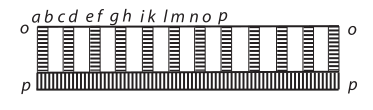
\includegraphics[trim = 0mm -3mm -5mm 0mm, clip, width=0.5\textwidth]{images/lh0351502_10r-d1.pdf}\\
%\rule[0pt]{13mm}{0mm}[\textit{Fig. 1, nach Hooke Fig. 28}]
%\end{wrapfigure}
Palus Mareotis\protect\index{Sachverzeichnis}{Palus Mareotis}, aut Lacus niger\protect\index{Sachverzeichnis}{Lacus Niger}, duae nigrae maculae in campo lucido, sunt plus quam minuti. Experimentum quod probat vim oculi limitatam, sume folium chartae albae duc in longitudinem duas parallelas oo, pp. distantia 4 aut 5 pollicum. Duc plures alias rectas ad has perpendiculares per puncta ipsius oo, transeuntes nempe per \textit{a. b. c. d. e. f. g. h. i. k. l. m. n.} \edtext{\textit{o.}}{\lemma{}\Bfootnote{\textit{o. erg. L}}} \textit{p.} distantia pollicis una ab altera. Spatia intercepta sint alternatim alba et nigra: affige parieti in radiis solis, et recede ad distantiam circiter 287 \rule[-4mm]{0mm}{10mm}$\displaystyle\frac{1}{3}$ pedum, plus minusve, ut quousque discernere potes. Ut autem distinguere possit, necesse est ut possit numerare. Haec distantia dabit virtutem oculi cujusque, unde judicari potest quantus angulus videri possit nudo visu, distincte. Altitudines solis sumi possunt ad secundi minuti exactitudinem, communi visu, si instrumentum satis largum; Nam imago solis transmissa per foramen rotundum ope superioris dioptrae\protect\index{Sachverzeichnis}{dioptra}, est repraesentata intra circulum upon the lower sight; et ope oculorum huic dioptrae\protect\index{Sachverzeichnis}{dioptra} appropinquantium, fieri potest per instrumenta satis magna, ut ad exactitudinem secundi minuti perveniatur. \edtext{Item [quodam] modo}{\lemma{Item}\Bfootnote{\textit{(1)}\ quomad \textit{(2)}\ \textbar\ quomam \textit{ \"{a}ndert Hrsg.} \textbar\ modo \textit{L}}} et in luna, cum est valde clara \edtext{quod in aliis corporibus coelestibus nemo fecit. Sed et haec via}{\lemma{clara}\Bfootnote{\textit{(1)}\ sed etiam haec ipsa via a \textit{(2)}\ quod [...] via \textit{L}}} telescopiis\protect\index{Sachverzeichnis}{telescopium} melius fieri potest, solo radii tripedalis instrumento quod fieri curavi, faciam observationes decies\\
\pend
\setline{26}
\vspace{0.5em}
\pstart
\begin{center}  
   \hspace{13mm} 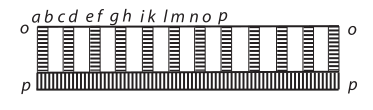
\includegraphics[trim = 0mm 5mm 0mm 0mm, clip, width=0.55\textwidth]{images/lh0351502_10r-d1.pdf}
\newline
\centering
[\textit{Fig. 1, nach Hooke Fig. 28}]
\end{center}  
\pend
\newpage
\pstart \noindent accuratiores; exceptis solaribus \edtext{quam maximis Hevelianis}{\lemma{}\Bfootnote{quam maximis Hevelianis \textit{erg. L}}} quanta ad pinnacidia quadrantis\protect\index{Sachverzeichnis}{quadrans} aenei Heveliani de quibus \edtext{pag. 98.}{\lemma{pag. 98.}\Cfootnote{\textsc{J. Hevelius}, \textit{Machinae Coelestis Pars Prior}, Danzig 1673, S. 98.\cite{00329}}} ille pro altitudine solis sumenda, haec bene quidem; sed \edtext{meliora adhibito}{\lemma{}\Bfootnote{meliora \textbar\ si \textit{gestr.}\ \textbar\ adhibito \textit{L}}} vitro objectivo, etiam sine Tubo. Ita semi quam voluisset \edtext{dedisset magnitudinem superiori dioptrae\protect\index{Sachverzeichnis}{dioptra} et imagini solis}{\lemma{dedisset}\Bfootnote{\textit{(1)}\ claritatem radiis solis \textit{(2)}\ magnitudinem [...] solis \textit{L}}}, idque sine specie penumbrae\protect\index{Sachverzeichnis}{penumbra}, posito inferiorem dioptram\protect\index{Sachverzeichnis}{dioptra} debita distantia vitri objectivi. Divisio Tychonica\protect\index{Sachverzeichnis}{divisio Tychonica} hodie vulgo nota, per diagonales, quae parallelos circulos secant, hanc ipse Tycho\protect\index{Namensregister}{\textso{Brahe}, Tycho 1546-1601} tribuit Anglico Mathematico Canzlero\protect\index{Namensregister}{\textso{},}. Observavit Hevelius\protect\index{Namensregister}{\textso{Hevelius}, Johannes (1611-1687)} instrumenta ex parte lignea, tamen subjecta esse errori; itaque fieri curavit ex metallo solido; ait tamen Hookius\protect\index{Namensregister}{\textso{Hooke}, Robert (1635-1703)} Christophorum Wrennum\protect\index{Namensregister}{\textso{Wren}, Christopher (1632-1723)} fecisse satis bona, modo laminae divisiones recipientes ex metallo. Caeterum ex instrumentis Hevelius\protect\index{Namensregister}{\textso{Hevelius}, Johannes (1611-1687)} recipit tantum sextantes\protect\index{Sachverzeichnis}{sextans}, Quadrantes\protect\index{Sachverzeichnis}{quadrans}, Octantes, rejectis: Radiis, Astrolabiis, Zodiacalibus vel Aequinoctialibus annulis, parallacticalibus instrumentis or Hoops nos tamen inquit Hook\protect\index{Namensregister}{\textso{Hooke}, Robert (1635-1703)} infra ostendemus, quosdam ex iis esse necessarios. Methodum subdividendi quadrantem\protect\index{Sachverzeichnis}{quadrans} ab Hedraeo\protect\index{Namensregister}{\textso{Hedraeus}, Bengt (1608-1659)} in praxin traductam magni facit Hevelius\protect\index{Namensregister}{\textso{Hevelius}, Johannes (1611-1687)}. Benedictus Hedraeus\protect\index{Namensregister}{\textso{Hedraeus}, Bengt (1608-1659)} 1643\cite{00330} \edtext{librum}{\lemma{librum}\Cfootnote{\textsc{B. Hedraeus}, \textit{Nova et accurata astrolabii geometrici structura}, Leiden 1643.\cite{00330}}} edidit circa novam et accuratam [10~v\textsuperscript{o}] structuram Astrolabii Geometrici.
\pend 
%    \count\Afootins=1200
\count\Bfootins=1200
\count\Cfootins=1200
\pstart Hevelius\protect\index{Namensregister}{\textso{Hevelius}, Johannes (1611-1687)} ipse suas fecit divisiones sui Quadrantis\protect\index{Sachverzeichnis}{quadrans} aenei quem primo describit. Subdivisiones fecit modo Tychonico ductis circulis parallelis, sed distantias circulorum parallelorum fecit aequales, \edtext{in Tychone\protect\index{Namensregister}{\textso{Brahe}, Tycho (1546-1601)}}{\lemma{}\Bfootnote{in Tychone\protect\index{Namensregister}{\textso{Brahe}, Tycho (1546-1601)} \textit{erg. L}}} accuratius fecisset, ponendo eorum distantias \textit{according to the proportions of the differences of the secants of some ten minutes}, \edtext{[\textit{next}]}{\lemma{}\Bfootnote{\textit{nex L \"{a}ndert Hrsg.}}} \textit{successively following one another in some degree of the} \edtext{\textit{quadrant\protect\index{Sachverzeichnis}{quadrans}}}{\lemma{\textit{quadrant}}\Cfootnote{\textsc{R. Hooke}, \textit{Animadversions}, S. 12.}} \textit{wich} \edtext{[\textit{is}]}{\lemma{}\Bfootnote{\textit{is: erg. Hrsg. nach Vorlage}}} \textit{easie to determine from the distance of the two extream or bounding} \edtext{\textit{circles}}{\lemma{\textit{circles}}\Cfootnote{a.a.O., S. 12.}}. Sed modo spatium in quo jacent circuli sit valde largum, et modo partes graduum distinguendae sint exiguae; error ab aequalibus \edtext{distantiis contemnendus}{\lemma{}\Bfootnote{distantiis \textbar\ non \textit{gestr.}\ \textbar\ contemnendus \textit{L}}} praesertim pro nudo visu. Modus Hookii\protect\index{Namensregister}{\textso{Hooke}, Robert (1635-1703)} quo labor ad partem nonagesimam reduci potest: pro divisione per diagonales; nimirum divisio unius gradus serviet pro omnibus 90. Certior est quoque, et exactior. Est autem talis: sume frustum tenue, \textit{of a lookings glas} \edtext{\textit{platte}}{\lemma{\textit{platte}}\Cfootnote{a.a.O., S. 13.}}; speculi plani. Ab utraque parte lene politum ac laevigatum et satis largum d'un sens (of \textit{one} \edtext{\textit{way}}{\lemma{\textit{way}}\Cfootnote{a.a.O., S. 13.}},) ut tegere possit omnem illam quadrantis\protect\index{Sachverzeichnis}{quadrans} partem in qua diagonales fieri necesse est. In alteram autem plagam, seu alio sensu, teget duos aut tres gradus quadrantis\protect\index{Sachverzeichnis}{quadrans} \textit{(: This I do the bigger that the sides of the arm may} \edtext{\textit{not}}{\lemma{\textit{not}}\Cfootnote{a.a.O., S. 13.}} \edtext{[inumbrare]}{\lemma{}\Bfootnote{inumbare \textit{L \"{a}ndert Hrsg.}}} et obnigrare divisiones et numerationes. Vult credo dicere ideo \edtext{hanc vitream tabulam}{\lemma{hanc}\Bfootnote{\textit{(1)}\ laminam \textit{(2)}\ vitream tabulam \textit{L}}} a se tam fieri largam, ut sustentacula ejus sint satis remota ab illis numeris, quibus videndis opus habemus, quales sunt ipsi qui loco quo utimur, in quo dioptra\protect\index{Sachverzeichnis}{dioptra} ojectiva est, proximi sunt; ne tegant divisiones. :) Hanc jam tabulam prorsus ita divide, ut Hevelius\protect\index{Namensregister}{\textso{Hevelius}, Johannes (1611-1687)} divisit \edtext{[ipsum]}{\lemma{}\Bfootnote{ipsam \textit{L \"{a}ndert Hrsg.}}} ubique quadrantem\protect\index{Sachverzeichnis}{quadrans}, nisi quod si paulo largius est spatium illud, proportione \edtext{ad radium}{\lemma{ad}\Bfootnote{\textit{(1)}\ gradum \textit{(2)}\ radium \textit{L}}} circuli paralleli non sint aequidistantes, sed secundum Tabulam tangentium aut secantium naturalium elaborati. Has divisiones facies circinis quorum pedum extrema adamantibus instructa, qualibus utuntur et vitrarii. Itaque divisiones fac, et duc lineas et pone \textit{in the frame of the} \edtext{\textit{ruler}}{\lemma{\textit{ruler}}\Cfootnote{a.a.O., S. 14.}} (formam vel regulae) ita ut latus linearum immediate tangat quadrantem\protect\index{Sachverzeichnis}{quadrans}. Ipse aeneus quadrans divisus sit in 90 partes aequales vel gradus et ex quolibet puncto divisionis rectae ad circumferentiam ductae per totam quadrantis\protect\index{Sachverzeichnis}{quadrans} faciem seu usque ad ipsum centrum \edtext{vel saltem quousque pertingunt}{\lemma{centrum}\Bfootnote{\textit{(1)}\ si scilicet eousque pertingunt \textit{(2)}\ vel saltem quousque pertingunt \textit{L}}} divisiones pro diagonalibus in vitro. \edtext{\textit{The frame}}{\lemma{\textit{The frame}}\Cfootnote{a.a.O., S. 14.}}, (forma sustentaculum) cujus ope movetur vitrum, est conveniens cavitas relicta in mobili brachio quadrantis\protect\index{Sachverzeichnis}{quadrans}. Figura, inquit, haec reddet clariora. Distantiae parallelorum circulorum secundum numeros tangentium et secantium naturales \edtext{[sumentur]}{\lemma{}\Bfootnote{sumetur \textit{L \"{a}ndert Hrsg.}}} \textit{with a pair of} \edtext{\textit{compasses}}{\lemma{\textit{compasses}}\Cfootnote{a.a.O., S. 14.}}, pari circinorum (+ cur pari seu duobus? +) \textit{contrived like} \edtext{\textit{beam-compasses\protect\index{Sachverzeichnis}{beam-compass}}}{\lemma{\textit{beam-compasses}}\Cfootnote{a.a.O., S. 14.}} (beam, statera, bilanx). Sed quorum puncta ad distantiam datam ponuntur ope cochleae quae movetur super una parte \edtext{\textit{of the beam}}{\lemma{\textit{of the beam}}\Cfootnote{a.a.O., S. 14.}}. Quod forte alibi describam clarius. 
\pend 
\count\Bfootins=1500
\count\Cfootins=1500
\pstart Si haec ratio non placet, pergit Hookius\protect\index{Namensregister}{\textso{Hooke}, Robert (1635-1703)}, \textso{alia} adhiberi potest, cujus ope feci exigua instrumenta valde exiguarum divisionum, valdeque exacta et facilia. Primum limbum (planum, latus) quadrantis\protect\index{Sachverzeichnis}{quadrans} dividendi reddo summe planum, \edtext{inde super}{\lemma{}\Bfootnote{inde \textbar\ inde \textit{streicht Hrsg.} \textbar\ super \textit{L}}} eo describo circulum ita levem ac subtilem, ut non nisi discerni possit, et ope Laminae divisoriae communis satis longae, radii decem pedum, divido in 90 partes, inde singulari artificio punctorum quorundam curiosorum, \textit{that strikes with a} \edtext{\textit{spring}}{\lemma{\textit{spring}}\Cfootnote{a.a.O., S. 14.}} (quae ope elaterii tundunt seu percutiunt) quae in alio discursu describo notantur gradus in lamina per curiosas exiguas, rotundas, profundas cavitates; haec per aliam lineam extra, divisam et figuratam communi more, distinguuntur et numerantur per figuras (+ numeros, cyphras +) communi more. Inde pro subdivisionibus facio exiguum \edtext{\textit{Hold-fast\protect\index{Sachverzeichnis}{hold-fast}}}{\lemma{\textit{Hold-fast}}\Cfootnote{a.a.O., S. 14.}}, (Tenaculum\protect\index{Sachverzeichnis}{tenaculum}, Estoc) firmatum per coch\-leam, fixum ad mobile quadrantis\protect\index{Sachverzeichnis}{quadrans} brachium, quod inservit ad tenendum extremum diagonalis crinis vel capilli, cujus alterum extremum super gradum \edtext{supplementarium donec}{\lemma{}\Bfootnote{supplementarium \textbar\ (. \Denarius\ .) \textit{gestr.}\ \textbar\ donec \textit{L}}} directe jaceat super aliqua cavitate subtilium divisionum limbi quadrantis\protect\index{Sachverzeichnis}{quadrans}. Hoc dat subdivisiones quadrantis\protect\index{Sachverzeichnis}{quadrans} quanta volo exactitudine. \textso{Supplementarius gradus} est gradus ingentis circuli, positus super exigua regula mobili, fixus in latere brachii mobilis, cujus magnitudo et distantia hac proportione invenitur; scilicet ut extremum inter distantiam exigui tenaculi et circuli punctati, est ad radium ejus circuli ita fiat distantia inter dictum extremum et supplementarium circulum, ad hujus circuli radium. Subjicit descriptionem, cum figura, sed figuram non invenio in exemplari meo, forte, quia deest una ex Tabulis autographicis. Describam tamen. Sit $aaa$ in figura \edtext{[32\textsuperscript{da}]}{\lemma{}\Bfootnote{30\textsuperscript{ma}\textit{\ L und Vorlage, \"{a}ndert Hrsg. nach Vorlage S. 78}}} repraesentans quadrantem\protect\index{Sachverzeichnis}{quadrans}, $b.bb$ subtilem circulum interiorem, descriptum super limbo quadrantis\protect\index{Sachverzeichnis}{quadrans} ex centro $l$ quem ope largi quadrantis\protect\index{Sachverzeichnis}{quadrans} radii decempedalis divido in gradus, et ope puncti elastici tundo in eo totidem exigua puncta, et numero 90 incipiendo ab $m$ et numerando ad $i$. Pone $dd$ repraesentare brachium mobile. \textit{cc} \edtext{\textit{the Hold-fast\protect\index{Sachverzeichnis}{hold-fast}}}{\lemma{\textit{the Hold-fast}}\Cfootnote{a.a.O., S. 15.}}, tenaculum\protect\index{Sachverzeichnis}{tenaculum}; fixum super latere ejus brachii. Hoc tenaculum ope exiguae cochleae tenet subtilem capillum, at $k$. \pend 
\pstart $ee$ est exigua regula fixa ad angulos rectos cum linea $lkf$. In hac linea (per puncta $l$ et $k$ \edtext{[\textit{through}]}{\lemma{}\Bfootnote{\textit{trough L \"{a}ndert Hrsg.}}} \textit{the points $l$ and $k$.)}\edtext{}{\lemma{\textit{and} $k$.)}\Cfootnote{a.a.O., S. 15.}} sumo punctum, ut $f$ et per $fI$ describo (+ distingue $l.i.I.$ +) partem circuli $fg$ cujus centrum est alicubi in linea $fkl$ producta, quod invenio resolvendo hanc proportionem, ut $ki$ ad $li$ ita $kf$ erit ad radium supplementarii circuli $fg$ quod cadet alicubi in $fkl$ productam, versus $l$. Inde sume gradum ejus circuli, qui extendetur ab $f$ ad $g$ et divide in divisiones tam minutas quam videtur opus, et numera ab $f$ ad $g$ nunc invenias quem angulum dioptra\protect\index{Sachverzeichnis}{dioptra} $dd$ facit cum dioptra\protect\index{Sachverzeichnis}{dioptra} $mm$ extendo pilum $hk$ donec inveniam jacere super proximo divisionis puncto versus dextram, et observo in regula $ee$ quae pars gradus ibi notata, et ad circulum $bbb$ quis gradus ibi notatus, summa utriusque dat veram mensuram anguli $ddlm$. Sed haec inquit obiter, quae fusius describam in alio discursu, ubi varias exhibebo rationes mechanicas et practicas dividendi accurate lineas in ullum numerum assignabilem partium proportionalium. Sed redeamus inquit ad quadrantem\protect\index{Sachverzeichnis}{quadrans} Hevelii\protect\index{Namensregister}{\textso{Hevelius}, Johannes (1611-1687)}. Is movetur ope cochlearum, sed alterandus pro variis azimuthis\protect\index{Sachverzeichnis}{azimuth}, quod nos infra evitabimus. \edtext{Idem Hookius\protect\index{Namensregister}{\textso{Hooke}, Robert (1635-1703)}}{\lemma{Idem}\Bfootnote{\textit{(1)}\ Hevelius \textit{(2)}\ Hookius \textit{(3)}\ Hookius \textit{L}}}, ego mox docebo modum quo unus observator potest sumere distantias in semicirculo exactius [11~r\textsuperscript{o}] multo quam possint duo, adeoque erit usui insigni pro nautis et astronomis. 
\pend 
%    \count\Afootins=1200
\count\Bfootins=1200
\count\Cfootins=1200
\pstart \edtext{Instrumenta metallina}{\lemma{Instrumenta}\Bfootnote{\textit{(1)}\ lignea \textit{(2)}\ metallina \textit{L}}}\protect\index{Sachverzeichnis}{instrumenta metallina}, nisi bene fortificata facilius curvantur, quam lignea crassa. Itaque ut maneant semper plana ponenda super tabula lignea vel forma \edtext{(\textit{frame})}{\lemma{\hspace{-0.5mm}(\textit{frame})}\Cfootnote{a.a.O., S. 18.\hspace{-3mm}}} fortificata contra curvationes, et in variis instrumenti partibus ope exiguarum cochlearum affirmanda ligno, tota interim \edtext{tabula aequilibrata}{\lemma{tabula}\Bfootnote{\textit{(1)}\ contre baton \textit{(2)}\ aequilibrata \textit{L}}}, ut facilius moveatur.
\pend 
\pstart Pro divisione per diagonales tandem elegit Hevelius\protect\index{Namensregister}{\textso{Hevelius}, Johannes (1611-1687)} divisionem aliam de qua scripsit Hedraeus\protect\index{Namensregister}{\textso{Hedraeus}, Bengt (1608-1659)}. Nempe Hevelius\protect\index{Namensregister}{\textso{Hevelius}, Johannes (1611-1687)} quadrantem\protect\index{Sachverzeichnis}{quadrans} facit non graduum 90 sed 110. pro habendis divisionibus cujuslibet gradus quadrantis\protect\index{Sachverzeichnis}{quadrans} ope \textit{of a new invented perpendicular of} \edtext{\textit{brass}}{\lemma{\hspace{-0.5mm}\textit{brass}}\Cfootnote{a.a.O., S. 20.\hspace{-3mm}}}. Putat Hedraeum\protect\index{Namensregister}{\textso{Hedraeus}, Bengt (1608-1659)} non esse inventorem, sed ex observatorio vel potius Repositorio Tychonis\protect\index{Namensregister}{\textso{Brahe}, Tycho (1546-1601)} habuisse. Erravere Hedraeus\protect\index{Namensregister}{\textso{Hedraeus}, Bengt (1608-1659)} et Hevelius\protect\index{Namensregister}{\textso{Hevelius}, Johannes (1611-1687)} quod credidere diagonales geometricae exactitudinis incapaces. Imo contra, diagonalis linea semper est pars tangentis, hoc est spatia inter parallelos circulos debent semper esse, \textit{in proportion to the difference of some tangent lines and the different distance of those circles from the center are alwayes to be in proportion of the difference of some tangent lines, and the different distance of those circles from the center}   
\textit{are alway in proportion of some} \edtext{\textit{secants:}}{\lemma{\hspace{-0.5mm}\textit{secants:}}\Cfootnote{a.a.O., S. 21.\hspace{-3mm}}} \edtext{Tycho}{\lemma{\textit{secants:}}\Bfootnote{\textit{(1)}\ \textit{and the way of f} \textit{(2)}\ Hevelius \textit{(3)}\ Tycho \textit{L}}} in \edtext{fine \textit{Mechanicorum}}{\lemma{\hspace{-0.5mm}fine \textit{Mechanicorum}}\Cfootnote{\textsc{T. Brahe}, \textit{Astronomiae instauratae mechanica}, Wandesburg 1598 (nicht paginiert), Abschnitt \glqq Supplementum de subdivisione et dioptris instrumentorum\grqq~beginnend auf der drittletzten Seite (\textit{TBO} V, S. 153-155).}} demonstrat errorem esse perexiguum diagonalium etiam interstitiorum aequalium. Sed facillime vera et naturalis habetur divisio, si proponatur $BC$ repraesentare diagonalem lineam subtendentem angulum 10' ad centrum $A$. Producatur linea $BC$ ad $F$, et cadat perpendicularis a centro $A$ ad $E$. Supponatur angulus ad $B$ unius gradus erit $BE$ tangens graduum 89. radio posito $AE$. Et $EC$ tangens \edtext{\textit{88,50'}}{\lemma{\textit{88,50'}}\Cfootnote{\textsc{R. Hooke}, \textit{Animadversions}, S. 23.}} et differentiae tangentium \textit{88,50'. 88,51'. 88,52' 88,53'. 88,54'. 88,55'. 88,56'. 88,57'. 88,58'.} \edtext{\textit{88,59' et 89.}}{\lemma{\textit{88,59' et 89.}}\Cfootnote{a.a.O., S. 23.}} dant distantias circulorum: \textit{C. 1. 2. 3. 4. 5. 6. 7. 8. 9.} \edtext{\textit{B}}{\lemma{\textit{B}}\Cfootnote{a.a.O., S. 23.}} (NB. non posui omnes numeros in figura.) Alia \edtext{methodo intervalla}{\lemma{methodo}\Bfootnote{\textit{(1)}\ haec \textit{(2)}\ intervalla \textit{L}}} assignat Hevelius\protect\index{Namensregister}{\textso{Hevelius}, Johannes (1611-1687)} ingeniosa et accurata. Aliam methodum continet Wallisius\protect\index{Namensregister}{\textso{Wallis}, John (1616-1703)} in Epistola ad Hevelium\protect\index{Namensregister}{\textso{Hevelius}, Johannes (1611-1687)}, quam inseruit Hookius\protect\index{Namensregister}{\textso{Hooke}, Robert (1635-1703)} dissertationi suae, sed non videtur ita expedita. 
\pend 
\newpage
\pstart
\noindent
\begin{wrapfigure}[17]{l}{0.44\textwidth}   
\vspace{-8mm}                 
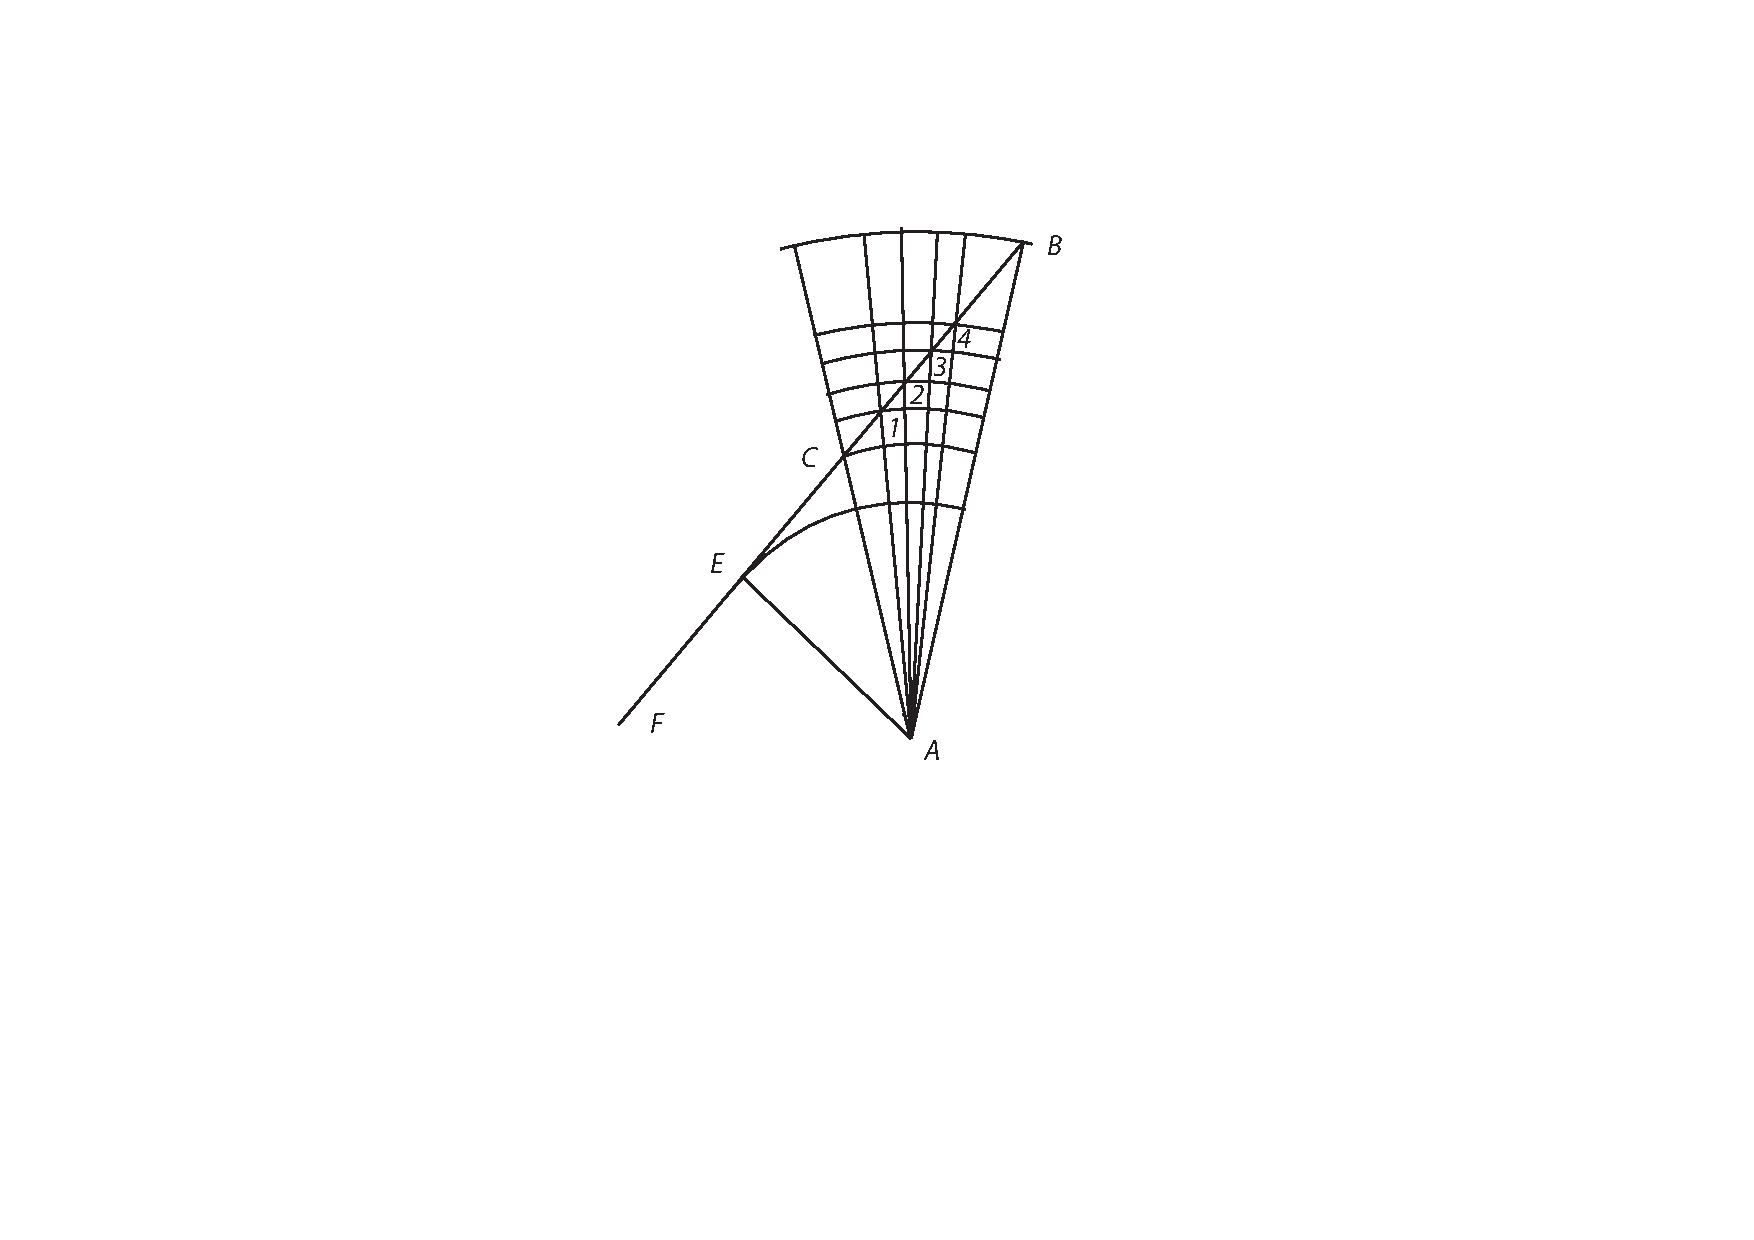
\includegraphics[trim = 0mm 2mm 0mm 0mm, clip, width=0.44\textwidth]{images/lh0351506_11r-d1.pdf}\\
\centering \rule[0pt]{0mm}{0pt}[\textit{Fig. 2, nach Hooke Fig. 35}]
\end{wrapfigure}
\textit{Pierre Vernier}\protect\index{Namensregister}{\textso{Vernier}, Pierre (1580-1635)} \textit{Capitain et chastelain pour sa Mt\'{e}}\protect\index{Namensregister}{\textso{Philipp III. K\"{o}nig von Spanien (1598-1621)}, Philipp IV. K\"{o}nig von Spanien (1621-1665)} \textit{au chasteau Dornans}\protect\index{Ortsregister}{Ornans} \textit{Conseiller et General de ses monnoyes au Comt\'{e} de} \edtext{\textit{Bourgogne}\protect\index{Ortsregister}{Burgund}}{\lemma{\textit{Bourgogne}}\Cfootnote{a.a.O., S. 30.}} \`{a} Brusselles\protect\index{Ortsregister}{Br\"{u}ssel} chez Fran\c{c}ois Vivien\protect\index{Namensregister}{\textso{Vivien}, Fran\c{c}ois}. Le titre du \edtext{liure}{\lemma{liure}\Cfootnote{\textsc{P. Vernier}, \textit{La Construction, l'usage et les propri\'{e}tez du quadrant\protect\index{Sachverzeichnis}{quadrans} nouveau de math\'{e}matique}, Br\"{u}ssel 1631.}} est: \textit{La construction l'usage et les proprietez du quadrant\protect\index{Sachverzeichnis}{quadrans} 
nouueau mathematique, comme aussi la construction de la table des sinus de minute en minutes successivement par une seule maxime. 
De plus un abreg\'{e} des dites tables en une petite demy-page, avec son usage, et en fin la methode de trouuer les angles d'un triangle par la connoissance des costez, et les costez par les angles, sans aide d'aucune Table}.
\\
\indent
Methodus descripta a Hookio pro faciendo catalogo fixarum accuratissimo vix decima laboris parte et temporis, et multo exactius: Fiat largus quadrans muralis vel potius semicirculus radii triginta pedum fixus exacte in meridiano\protect\index{Sachverzeichnis}{meridian} in muro ex quadratis lapidibus, bene junctis \textit{and cramped together,}\edtext{}{\lemma{\textit{together},}\Cfootnote{\cite{00332}\textsc{R. Hooke}, \textit{Animadversions}, S. 32.}} et positis super fundamento, firmo et solido \textit{to prevent all manner of slacking and swarfing. The rim of his}\edtext{}{\lemma{\textit{his}}\Cfootnote{a.a.O., S. 32.}} sit ex laminis aeneis in debito situ locatis ope ferreorum (barres) baculorum in muro fixorum, \textit{by running them with lead}\edtext{}{\lemma{\textit{lead}}\Cfootnote{a.a.O., S. 32.}} (+ cum plumbo infuso). Diviso hoc semicirculo in 180 gradus, et subdiviso quolibet gradu ope diagonalium super bene polita vitri tabula, divisa per minuta et secunda modo supra descripto: his factis adaptetur et Telescopium\protect\index{Sachverzeichnis}{telescopium} triginta pedum, ita ut Tubus non curvetur, nec vitrum excedat vero situ. Focus vitri objectivi sit \edtext{exacte \textit{upon the edge}}{\lemma{exacte}\Bfootnote{\textit{(1)}\ super uno edge \textit{(2)}\ \textit{upon the edge} \textit{L}}} (acies) \textit{of the brass limb,}\edtext{}{\lemma{\textit{limb,}}\Cfootnote{a.a.O., S. 32.}} limbi aenei ita ut ope ocularis\protect\index{Sachverzeichnis}{ocular}, quod est \textit{a deep convex}\edtext{}{\lemma{\textit{convex}}\Cfootnote{a.a.O., S. 32.}} punctualis locus vel altitudo stellae ad quartam pili latitudinis partem possit observari. Impedimentum curvaturae Telescopii\protect\index{Sachverzeichnis}{telescopium} fieri potest eo fere modo quem communicavi Hevelio\protect\index{Namensregister}{\textso{Hevelius}, Johannes (1611-1687)}, et \edtext{quem descriptum}{\lemma{}\Bfootnote{quem \textbar\ large \textit{gestr.}\ \textbar\ descriptum \textit{L}}} invenies apud ipsum. Excepto quod \edtext{\textit{instead of Ropes}}{\lemma{\textit{instead of Ropes}}\Cfootnote{a.a.O., S. 33.}} (loco restium) nunc commendo totidem braces (fibulas armillas) ligneas. Et licet non obstante omni diligentia evitari nequeat ut tubus in medio nonnihil curvetur, sed hoc non vitiabit observationem, quia vitrum objectivum eundem semper situm servat ad centrum, et focus ejus est exacte \edtext{\textit{in the edge of the limb}}{\lemma{\textit{limb}}\Cfootnote{a.a.O., S. 33.}}. Inconvenientia respiciendi \edtext{sursum inque}{\lemma{sursum}\Bfootnote{\textit{(1)}\ in lim \textit{(2)}\ inque \textit{L}}} alio \edtext{situ incommodo}{\lemma{situ}\Bfootnote{\textit{(1)}\ indebito \textit{(2)}\ incommodo \textit{L}}} \edtext{[praevenietur]}{\lemma{}\Bfootnote{prevenietur \textit{L \"{a}ndert Hrsg.}}} ope reflexi metalli cujus ope semper respicietur horizontaliter, hoc est perpendiculariter ad planum muri vel quadrantis\protect\index{Sachverzeichnis}{quadrans}. Et ut praeveniatur labor movendi (ope longi ligni) \edtext{ope \textit{of}}{\lemma{}\Bfootnote{ope \textit{of} \textit{erg. L}}} \textit{a long yard poysed upon centers on a frame before the said instrument}\edtext{}{\lemma{\textit{instrument}}\Cfootnote{a.a.O., S. 33.}}. Tubus brachium cum dioptra\protect\index{Sachverzeichnis}{dioptra} et sedes observatoris cui insidet simul possunt esse aequilibrata, ita ut circumagendo a \edtext{\textit{Windle,}}{\lemma{\textit{Windle},}\Cfootnote{a.a.O., S. 33.\hspace{15mm}}} facile sit movere se ad ullum situm desideratum. Objectivum est exacte ante centrum, et oculare\protect\index{Sachverzeichnis}{ocular} directe respicit divisiones limbi. Hac ratione observationes unius noctis sumi possunt aliquot centenarum \edtext{stellarum declinationes\protect\index{Sachverzeichnis}{declinationes stellarum}}{\lemma{stellarum}\Bfootnote{\textit{(1)}\ observat \textit{(2)}\ declinationes \textit{L}}} ad secundum usque minutum, modo sint \edtext{duo}{\lemma{}\Bfootnote{duo \textit{erg.} \textit{L}}} assistentes qui notent quae vides. Et eodem tempore recta ascensio cujuslibet eorum sumi potest, ope horologii penduli circularis: \textit{a accurate compound circular \textso{pendulums-clock\protect\index{Sachverzeichnis}{pendulum-clock}}},\edtext{}{\lemma{\textit{\textso{pendulums-clock}},}\Cfootnote{a.a.O., S. 33.}} quod alias describam notans ad secundum usque minutum appulsum cujusque stellae ad meridianum\protect\index{Sachverzeichnis}{meridian}, cumque objici posset refractione aeris variaturas declinationes earum stellarum\protect\index{Sachverzeichnis}{declinationes stellarum} quae \edtext{sunt meridionales}{\lemma{sunt}\Bfootnote{\textit{(1)}\ in ax \textit{(2)}\ meridionales \textit{L}}} valde, attamen cum hoc instrumentum viam suppeditet supra aliud quod sit in mundo, pro detegendis diversis refractionibus \edtext{aeris pro variis supra horizontem altitudinibus, usque ad secundi}{\lemma{aeris}\Bfootnote{\textit{(1)}\ ad sec \textit{(2)}\ pro [...] secundi \textit{L}}} exactitudinem sumendo altitudinem harum stellarum \textit{as never set in the North}\edtext{}{\lemma{\textit{North}}\Cfootnote{a.a.O., S. 34.}} in maxima et minima altitudine supra horizontem; Tabula harum refractionum facile rectificabit declinationem aliarum fixarum ad magnam altitudinem. 
\pend 
\count\Afootins=1200
\count\Bfootins=1200
\count\Cfootins=1200
\pstart Ad instrumentum\protect\index{Sachverzeichnis}{instrumentum Hevelii} Hevelii\protect\index{Namensregister}{\textso{Hevelius}, Johannes (1611-1687)} quo altitudines \edtext{meridianis\protect\index{Sachverzeichnis}{meridian} sumere praetendit}{\lemma{meridianis}\Bfootnote{\textit{(1)}\ sumit \textit{(2)}\ sumere praetendit \textit{L}}} ad secundum usque minutum, \edtext{respondet Hookius}{\lemma{respondet}\Bfootnote{\textit{(1)}\ Hevelius \textit{(2)}\ Hookius \textit{L}}} secundum minutum in eo instrumento esse ter millesimam pollicis partem quam nudus visus discernere nequeat et aegre Microscopio adjutus. Sed quomodo inquit discernet penumbram\protect\index{Sachverzeichnis}{penumbra}, quae non est certa ad minutum usque. Et quanquam dici queat, \textit{it is the same, round the circle, and the circle is the true bigness of the sun,}\edtext{}{\lemma{\textit{sun},}\Cfootnote{a.a.O., S. 35.}} ita ut circulus magnitudinis respondentis diametro solis\protect\index{Sachverzeichnis}{diametrus solis} et distantiae inferioris dioptrae\protect\index{Sachverzeichnis}{dioptra} a superiori, super ipsa inferiore describatur necesse esse [11~v\textsuperscript{o}]
%    %[11~v\textsuperscript{o}] 
\hspace{-1.8mm}ut definiat limbum solis, et ita facile esse discernere, quando is circulus perfecte repletus est figura solis per superiorem dioptram\protect\index{Sachverzeichnis}{dioptra} admissa. Respondeo hoc videri probabile et facile, et ita credi atque asseri ab omnibus Opticae scriptoribus. Sed rem plane aliter se habere. Nam praeterquam quod apud omnes in confesso est, penumbram\protect\index{Sachverzeichnis}{penumbra} hujus circuli minimum tam esse crassam quam diametrum superioris foraminis per quod trajectus est, quod non potest esse minus minuto: praeter hoc inquam, rem aliter demonstrat experientia, et quod limbus imaginis pictae super inferiore dioptra\protect\index{Sachverzeichnis}{dioptra}, terminatus est penumbra\protect\index{Sachverzeichnis}{penumbra}, quae est aliquando quinquies vel sexies crassior diametro foraminis, et quod est mirabilius, quo minus est foramen eo crassior est penumbra\protect\index{Sachverzeichnis}{penumbra}, \textit{and the bigger (to a certain degre) the less}\edtext{}{\lemma{\textit{less}}\Cfootnote{a.a.O., S. 35.}}. Sed nulla est crassities quae eam plane auferat, et diameter solis\protect\index{Sachverzeichnis}{diameter solis} ea ratione sumtus est aliquando crassior, aliquando tenuior, quam opus est, idque satis notabiliter. Sed de hac aliisque lucis miris proprietatibus alias \edlabel{hookius1}dicam. 
\pend 
\pstart \edtext{Hevelius\edlabel{hookius2}}{{\xxref{hookius1}{hookius2}}\lemma{dicam.}\Bfootnote{\textit{(1)}\ Hookius ope duarum cochlearum manualium \textit{(2)}\ Hevelius \textit{(3)}\ Hevelius \textit{L}}} usus refert quos admirabiles ait, cochlearum imo in locando et fixando quadrante\protect\index{Sachverzeichnis}{quadrans}, 2\textsuperscript{o} in danda motione qua sequamur instrumento solem et fixas in diurno eorum motu, 3\textsuperscript{o} in subdivisionibus graduum usque ad 2\textsuperscript{da} minuta. Sed putat Hookius\protect\index{Namensregister}{\textso{Hooke}, Robert (1635-1703)} pro sequendo stellarum motu, incommodum esse usum cochlearum et rectius adhiberi Automaton\protect\index{Sachverzeichnis}{automaton exiguum} \edtext{exiguum, cujus ope instrumentum semel positum ad stellae Azimuth\protect\index{Sachverzeichnis}{azimuth} exacte}{\lemma{exiguum,}\Bfootnote{\textit{(1)}\ quod satis exacte \textit{(2)}\ cujus [...] exacte \textit{L}}} pro aliquot horis sequatur stellae motum. Quod attinet subdivisiones ope cochlearum, addit \edtext{Hookius\protect\index{Namensregister}{\textso{Hooke}, Robert (1635-1703)} id}{\lemma{Hookius}\Bfootnote{\textit{(1)}\ non \textit{(2)}\ id \textit{L}}} verum esse, sed non bene factum ab Hevelio\protect\index{Namensregister}{\textso{Hevelius}, Johannes (1611-1687)} quia non est certus an ab initio suam cochleam ad certum aliquem gradum fixerit concludit Hookius\protect\index{Namensregister}{\textso{Hooke}, Robert (1635-1703)} de primario illo Hevelii\protect\index{Namensregister}{\textso{Hevelius}, Johannes (1611-1687)} quadrante\protect\index{Sachverzeichnis}{quadrans} (quem ille \edtext{pag. 184}{\lemma{pag. 184.}\Cfootnote{\textsc{J. Hevelius}, \textit{Machina Coelestis}, Danzig 1673\cite{00329}, S. 184, Vergleich der Quadranten\protect\index{Sachverzeichnis}{Quadrant} des Hevelius und des Brahe.}} commendat) videri \textit{the frame}\edtext{}{\lemma{\textit{the frame}}\Cfootnote{\textsc{R. Hooke}, \textit{Animadversions}, S. 37.}} structuram instrumenti ejus valde bonam, et ope quarundam additionum, ut quoad dioptras\protect\index{Sachverzeichnis}{dioptra}, divisiones, perpendicula et erectiones, debere tam fieri bonam, quam opus est pro ullo usu Astronomico; et quadragies meliore quam nunc factum et descriptum est ab \edtext{Hevelio\protect\index{Namensregister}{\textso{Hevelius}, Johannes (1611-1687)}. Nam}{\lemma{Hevelio.}\Bfootnote{\textit{(1)}\ Sed \textit{(2)}\ Nam \textit{L}}} ita ut est, et ab Hevelio\protect\index{Namensregister}{\textso{Hevelius}, Johannes (1611-1687)} datur, non est melius largo instrumento quod Tycho\protect\index{Namensregister}{\textso{Brahe}, Tycho (1546-1601)} adhibuerat 100 abhinc annis, et inferius ejus quadrante\protect\index{Sachverzeichnis}{quadrans} murali pro sumendis altitudinibus meridianis\protect\index{Sachverzeichnis}{meridian}. 
\pend 
\pstart Ingenue fatetur \edtext{Hevelius}{\lemma{fatetur}\Bfootnote{\textit{(1)}\ Tycho \textit{(2)}\ Hevelius \textit{L}}} difficultatem in sumendis distantiis fixarum a luna; quod a nulla alia re provenit, quam imperfectione visus communis et omnes difficultates evanescent, si dioptrae\protect\index{Sachverzeichnis}{dioptra} fiant aliter (Telescopice\protect\index{Sachverzeichnis}{telescopium}). Et videtur longe majorem adhuc facere difficultatem, sumere distantiam solis a \venus\ visa diurno tempore, sed ego mox dicam methodum per quam non tantum facile sit sumere eam a \venus, sed et a \mars\ et \jupiter, \textit{nay, from several of the fix Stars.}\edtext{}{\lemma{\textit{Stars}.}\Cfootnote{a.a.O., S. 38.}} 
\pend 
\count\Afootins=1500
\count\Bfootins=1500
\count\Cfootins=1500
\pstart Non dubito Hevelium\protect\index{Namensregister}{\textso{Hevelius}, Johannes (1611-1687)} exactissimum fuisse, quantum nudo visu licet. Sed optarem videre distantias quas dicit sumsisse octo fixarum prope Eclipticam\protect\index{Sachverzeichnis}{ecliptica}, nempe: \textit{Lucidae Arietis, et Palilicii, Palilicii et Pollucis, Pollucis et Reguli, Reguli et Spicae, Spicae et in manu Serpentarii, in manu Serpentarii et Aquilae, Aquilae et Marchab, Marchab et Lucidae Arietis,}\edtext{}{\lemma{\textit{Arietis},}\Cfootnote{a.a.O., S. 38.}} idque tanta exactitudine, ut non defuerit ei secundum minutum in tota circumferentia circuli coelestis, octo observationibus sumta. Quod mihi videtur una ex maximis asseverationibus quas unquam viderim; et ausim geometrice demonstrare, quod fuerit ipsi certe, et instrumentis quibus usus est, impossibile fuisse facere vel unicam observationem 30 secundorum certitudine, unde fit ut in toto circulo vel 240 secundis certus fuerit, vel 4 minutis. Superest ut addam quaedam de \textso{apparatu meo}\protect\index{Sachverzeichnis}{apparatus Hookii}, ut patientiam lectoris compensem ac subjiciam, inquit, antea Hevelii\protect\index{Namensregister}{\textso{Hevelius}, Johannes (1611-1687)} \edtext{Epistolam}{\lemma{Epistolam}\Cfootnote{a.a.O., S. 39-41.}} ad Oldenburgium\protect\index{Namensregister}{\textso{Oldenburg}, Heinrich (ca. 1619-1677)}. Ait Hevelius\protect\index{Namensregister}{\textso{Hevelius}, Johannes (1611-1687)} in illa: \textit{Hocce penitus mihi imaginor, si totum istud negotium dioptris Telescopicis\protect\index{Sachverzeichnis}{telescopium} suscepissem, quod non solum plurimos annos examinibus trivissem, sed spe sine dubio varia via, de qua non est hic disserendi locus, cecidissem. Exinde gratulor mihi me ad eam sententiam nondum transiisse, ac mea methodo universa perfecisse}\edtext{}{\lemma{\textit{perfecisse}}\Cfootnote{a.a.O., S. 40.}}. Ubi viderint meas observationes judicent. \edtext{Integrum cuilibet}{\lemma{}\Bfootnote{Integrum \textbar\ postea \textit{ gestr.}\ \textbar\ cuilibet \textit{ L}}} erit, vel alium plane sua methodo catalogum construere adhibitis \textit{tot centenis novis fixis hactenus neglectis}\edtext{}{\lemma{\textit{neglectis}}\Cfootnote{a.a.O., S. 41.}}. Sed non video an cura haec quenquam adhuc serio tangat, facile est \textit{unam alteramve stellam ope Telescopii\protect\index{Sachverzeichnis}{telescopium} vel Telescopicarum\protect\index{Sachverzeichnis}{telescopium} dioptrarum\protect\index{Sachverzeichnis}{dioptra}, dum praecipuas ac majores fixas earumque intercapedines sumimus correctas ad debitum locum deducere, tum nonnunquam distantias nonnullarum stellarum capere, haec ludicra sunt. Sed omnes conjunctim secundum longum ac latum restituere, tum ductu continuo singulis serenis diebus ac noctibus tam altitudinum solarium quam reliquarum stellarum operam dare easque orbi exponere, ut pateat instrumentorum harmonia ac motuum certitudo, hoc artis, hoc laboris est. Quando observationes 20 vel 30 annorum spatio ab utraque parte}\edtext{}{\lemma{\textit{parte}}\Cfootnote{a.a.O., S. 41.}} habebimus, res clarior erit. \textit{Interea quilibet fruatur suo ingenio}\edtext{}{\lemma{\textit{ingenio}}\Cfootnote{a.a.O., S. 41.}} etc. Respondet Hookius\protect\index{Namensregister}{\textso{Hooke}, Robert (1635-1703)} errare Hevelium\protect\index{Namensregister}{\textso{Hevelius}, Johannes (1611-1687)} in eo, quod putat \edtext{ad}{\lemma{}\Bfootnote{ad \textit{erg. L}}} quamvis telescopicam\protect\index{Sachverzeichnis}{telescopium} observationem opus esse novo examine unde videri Hevelium\protect\index{Namensregister}{\textso{Hevelius}, Johannes (1611-1687)} non habere veram notionem de observationibus ejusmodi. \edtext{Usus sum}{\lemma{ejusmodi.}\Bfootnote{\textit{(1)}\ Item qu \textit{(2) }\ Usus sum \textit{L}}} quadrante\protect\index{Sachverzeichnis}{quadrans} sex pedum, instructo duabus dioptricis telescopicis\protect\index{Sachverzeichnis}{telescopium}, pro examinandis motibus cometis\protect\index{Sachverzeichnis}{cometa} anni 1665. Et cum eandem rem melius fecerim quadrante\protect\index{Sachverzeichnis}{quadrans} radii 6 pollicum, quam ille possit quadrante\protect\index{Sachverzeichnis}{quadrans} sex pedum, puto concludere minimum debuisse, eandem rem decies melius fieri posse in radio sex pedum. Instrumenta telescopicarum\protect\index{Sachverzeichnis}{telescopium} dioptricarum ope ad minuta tertia proferri possunt. Plus faciam unius \edtext{pedis radio}{\lemma{unius}\Bfootnote{\textit{(1)}\ instrumenti radii \textit{(2)}\ pedis radio \textit{L}}} sextante\protect\index{Sachverzeichnis}{sextans} aut quadrante\protect\index{Sachverzeichnis}{quadrans}, quam ille ope 60 pedum simplicibus dioptris. 
\pend 
\count\Afootins=1500
\count\Bfootins=1500
\count\Cfootins=1500
\pstart
%    [12~r\textsuperscript{o}] Pars 2\textsuperscript{da} Excerptorum ex Hookio\protect\index{Namensregister}{\textso{Hooke}, Robert (1635-1703)} contra Hevelium\protect\index{Namensregister}{\textso{Hevelius}, Johannes (1611-1687)} 
\pend 
\count\Afootins=1200
\count\Bfootins=1200
\count\Cfootins=1200
\pstart Hactenus Hookius\protect\index{Namensregister}{\textso{Hooke}, Robert (1635-1703)} examinavit Instrumenta\protect\index{Sachverzeichnis}{instrumentum Hevelii} Hevelii\protect\index{Namensregister}{\textso{Hevelius}, Johannes (1611-1687)}, \edtext{nunc de suis quoque methodis loquitur. Ait}{\lemma{nunc}\Bfootnote{\textit{(1)}\ ait \textit{(2)}\ de suis [...] Ait \textit{L}}} se invenisse et in exiguis modulis tentasse aliquot \textit{scores}\edtext{}{\lemma{\textit{scores}}\Cfootnote{a.a.O., S. 44.}} (vicenas) modorum perficiendi instrumenta pro sumendis angulis, distantiis, altitudinibus, tabellis etc. quorum omnium usus esse possit in terra, quorundam et in mari. Et ultra eas quas expertus sit rationes, posse se describere aliquot centenas, (2, a 300) quorum quilibet sit aeque accuratus ac Hevelii largissimus et quidam 30, 40, imo 60 vicibus accuratiores. Omnes tamen a se invicem differentes, in quibusdam partibus essentialibus. Assevero me ultra 20 methodos (\textit{contrived}\edtext{}{\lemma{\textit{contrived}}\Cfootnote{a.a.O., S. 44.}}) adhibuisse dividendi instrumenta, quarum quaelibet aeque ab alia qualibet distincta, quam via Heveliana a via diagonalium et tamen quaelibet earum capax ejusdem minimum certitudinis et exactitudinis et quaedam, centies majoris. Habeo plus, quam duodenam modorum adaptandi instrumenta ad perpendicularitatem et horizontalitatem; omnia aeque exacta ac perpendiculum commune, et quaedam multo magis, et ad exactitudinem progredientia \textso{quantamvis}, valde differentia a se invicem. Habeo totidem differentia dioptrarum\protect\index{Sachverzeichnis}{dioptra} genera pro augendis, dirigendis, accommodandis et certificandis dioptris, quorum quaedam applicandae ad usus particulares, quaedam ad omnes, quarum ope etiam haec pars perfici potest ad certitudinem quantamvis. Varias habeo rationes fixandi instrumenta, et accommodandi pro hoc aut alio aut variis usibus. Varias habeo vias mechanicas pro ipsis illis machinis elaborandis magna facilitate, et certitudine: cognitio non minus utilis quam theoria et usus jam elaboratorum. Cum sint adeo pauci in mundo, qui possint hoc aut velint. Habeo viam mechanicam calculandi et efficiendi operationes Arithmeticas longe promtiorem et certiorem, quam fieri possit per logarithmos. Quod implet totum negotium dimetiendi angulos. 
\pend 
\pstart Describit ergo instrumentum pro angulis et distantiis coelestibus sumendis, quod magnitudine aucta tantae capax est exactitudinis, quantam aer et atmosphaera permittunt. 
\pend 
\newpage
\pstart Dioptra\protect\index{Sachverzeichnis}{dioptra} Hookii Telescopia\protect\index{Sachverzeichnis}{telescopium} ex duabus lentibus convexis\protect\index{Sachverzeichnis}{lens convexa}, in tubo vel pyxide quadrata, ponatur oculus ibi, \edtext{ubi totum vitrum oculare\protect\index{Sachverzeichnis}{ocular} ab objecto}{\lemma{}\Bfootnote{ubi \textbar\ ubi \textit{streicht Hrsg.} \textbar\ totum \textit{(1)}\ objectum a \textit{(2)}\ vitrum oculare\protect\index{Sachverzeichnis}{ocular} ab objecto \textit{L}}} repletum videt. In foco ponantur duo fila se decussantia, idque ita dignosces, si moto oculo moveri super objecto apparent fila non sint in foco, si fixa manent[,] sunt, ibi fila etsi subtilissima ex tela serica, apparent ut fila crassa tracti. 
\pend 
\pstart \textso{Modus dividendi}. Modo Tychonis\protect\index{Namensregister}{\textso{Brahe}, Tycho (1546-1601)} et Hevelii\protect\index{Namensregister}{\textso{Hevelius}, Johannes (1611-1687)} opus est 150 pedum radio pro secundis. Hic sufficit radius 3 pedum. Imo in tali instrumento non bene distinguentur divisiones nudo visu, hoc tam facile nudo visu quam facile cuilibet videre decimam pollicis partem. In instrumento 150 pedum minutum vix est semipollex, et secundum \rule[-4mm]{0mm}{10mm}$\displaystyle\frac{1}{120}$ pollicis quanquam autem Hevelius multa se praestare putet via Nonii\protect\index{Namensregister}{\textso{Nu\~{n}ez}, Pedro (1502-1578)}, Vernerii\protect\index{Namensregister}{\textso{Vernier}, Pierre (1580-1637)} vel Hedraei\protect\index{Namensregister}{\textso{Hedraeus}, Bengt (1608-1659)}, sed credo his quae dixit consideratis aliter censurum. Cum radius 10 pedum sit tantum hujus (150 pedum) pars \rule[-4mm]{0mm}{10mm}$\displaystyle\frac{1}{15}$ unde secundum minutum $\displaystyle\frac{1}{15,\smallfrown 120}$. Utitur Hookius\protect\index{Namensregister}{\textso{Hooke}, Robert (1635-1703)} \edtext{cochleis quas}{\lemma{cochleis}\Bfootnote{\textit{(1)}\ quarum \textit{(2)}\ quas \textit{L}}} circumagit ope indicis prorsus ut mihi relatum est fecisse jam \edtext{Hedraeum\protect\index{Namensregister}{\textso{Hedraeus}, Bengt (1608-1659)}. Habet}{\lemma{Hedraeum.}\Bfootnote{\textit{(1)}\ Ut legi facilius possint cha \textit{(2)}\ Hinc etiam facile na \textit{(3)}\  Habet \textit{L}}} ea methodus illud quoque compendium, \edtext{ut divisorii numeri non divisionibus}{\lemma{ut}\Bfootnote{\textit{(1)}\ divisoriae lineae non ipsi \textit{(2)}\ divisorii numeri non divisionibus \textit{L}}} illis subtilissimis ascribantur sed in indice revolutionis legantur; qui rursus quantalibet subtilitate subdivisus intelligi potest. Utque in indice facilius legantur potest extremum indicis secum ducere lentem, quae augeat characteres. 
\pend 
\pstart Aliud commodum proponit Hookius\protect\index{Namensregister}{\textso{Hooke}, Robert (1635-1703)}, quod est observatorem suum idque uno oculi \edtext{ictu dirigere instrumentum}{\lemma{ictu}\Bfootnote{\textit{(1)}\ praestare quantam \textit{(2)}\ dirigere instrumentum \textit{L}}} ad duo simul objecti loca vel quocunque angulo a se invicem remota sint, aut etiamsi sint in linea recta opposita; hoc est unum ex primariis auxiliis observationum, cum alia instrumenta duos requirant observatores pro sumendis coelestibus distantiis, et Tycho\protect\index{Namensregister}{\textso{Brahe}, Tycho (1546-1601)} illis usus sit quatuor, ubi opus erat concursu tam accurato, ut vel unius error omnia vitiaret. Et instrumenta pro uno observatore; qua duplici opus observatione, ob motum et mille mutationum incommoda ab omnibus relicta sunt. Hic vero nihil aliud faciendum est, quam ut ope cochleae moveatur instrumenti bracchium, donec sentiat ambo objecta se simul tangere, et in his punctis eorum distantiam metietur. Hoc quivis facile discet intellecta methodo adaptandi duo Telescopia\protect\index{Sachverzeichnis}{telescopium}, \textit{that by looking} \makebox[1.0\textwidth][s]{\textit{in at one small hole in the side of one of them, he will be able to see both those objects}}
\pend
\newpage
\pstart \noindent \textit{distinctly, to wich they are directed, how much soever separated.}\edtext{}{\lemma{\textit{separated}.}\Cfootnote{a.a.O., S. 56.}} Junge duo telescopia\protect\index{Sachverzeichnis}{telescopium} ope juncturae cavae, seu pertusae, cujus cavitas \rule[-4mm]{0mm}{10mm}$\displaystyle\frac{3}{4}$ cavitatis tuborum ipsorum Telescopiorum\protect\index{Sachverzeichnis}{telescopium}, et directe contrarie hujus cavitatis \edtext{in junctura}{\lemma{}\Bfootnote{in \textbar\ ipsa \textit{gestr.}\ \textbar\ junctura \textit{L}}} fiat junctura exigua circiter magnitudine nigerrimae partis pupillae oculi, ita ut oculus respiciens in hanc cavitatem possit videre perpendiculariter in tubum inferiorem, inde oblique pone duo \edtext{[frusta]}{\lemma{}\Bfootnote{frustra \textit{L \"{a}ndert Hrsg.}}} metalli reflectentis bene posita, ita ut reflectant axem utriusque tubi ad angulos rectos. Quod fit fixando planum laminarum sive Tabularum (\textit{plates}\edtext{}{\lemma{\textit{plates}}\Cfootnote{a.a.O., S. 56.}}) inclinatum ad illam axem angulo 45 graduum. Effice ut superior lamina reflexiva (\textit{reflex plate}\edtext{}{\lemma{\textit{reflex plate}}\Cfootnote{a.a.O., S. 56.}}) perveniat a superiore tubi latere, eo usque ut tangat \edtext{axem vel medium tubi}{\lemma{axem}\Bfootnote{\textit{(1)}\ Tubi medii \textit{(2)}\ vel medium tubi \textit{L}}} et effice ut inferior se extendat per totum Tubum, a summo ad fundum, et a latere uno ad aliud. Apparebit debite locata esse, \edtext{si introspiciendo}{\lemma{si}\Bfootnote{\textit{(1)} inspiciendo \textit{(2)} introspiciendo \textit{L}}} per foramen exiguum contra centrum juncturae duo foramina rotunda tubi apparebunt oculo coalescere in unum, ita ut oculus simul directe pervideat longitudines utriusque. Quo facto his tubis apta duo Telescopia\protect\index{Sachverzeichnis}{telescopium} cum convexis ocularibus\protect\index{Sachverzeichnis}{ocular}
%    \hspace{-0.6mm}[12~v\textsuperscript{o}] et fac, ut fila pro dioptris in eorum focis se intersecent ad crucem, ita ut utraque possint esse in debita ab oculo distantia, introspiciendo per foramen laterale, inde aperiendo tubos super dicta junctura ad aliquem angulum et introspiciendo per foramen laterale, distingues planissime, una eademque opera duo objecta, tubis directe illata, et ad oculum reflexa. \makebox[1.0\textwidth][s]{Haec ut clarius intelligantur, addatur delineatio eorum in plano. Fac ut \textit{aabb} in figura}
\pend
\vspace{1.2em}
\count\Afootins=1200
\count\Bfootins=1200
\count\Cfootins=1200
\begin{center}   
\centering                 
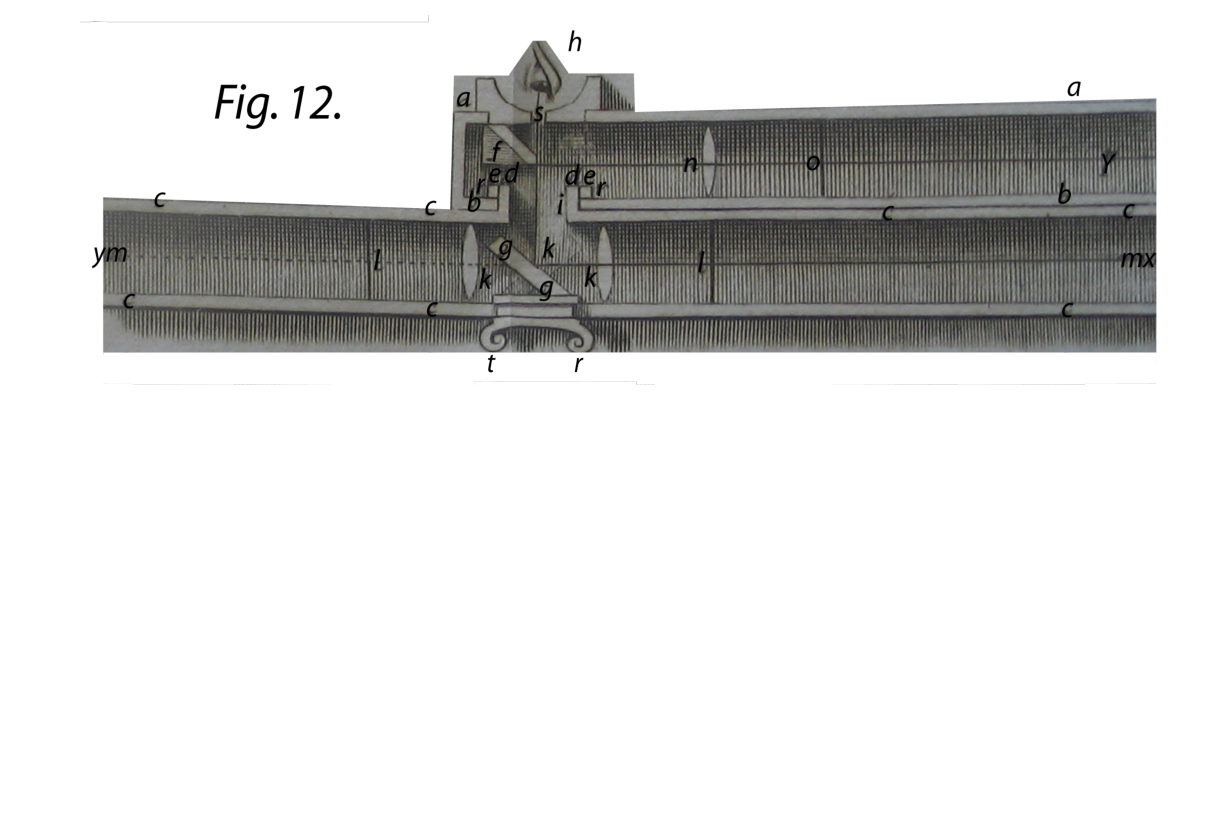
\includegraphics[trim = 0mm 1mm 0mm 2mm, clip, width=1.0\textwidth]{images/LH0351506_012v-dext12.pdf}\newline
\vspace*{3mm}\centering[\textit{Fig. 3; erg. Hrsg. nach Hooke Fig. 12}]
\end{center}
\pstart\noindent 12\textsuperscript{ma} 
\edtext{}{
%{\lemma{figura 12\textsuperscript{ma}}\Cfootnote{An dieser Stelle im Manuskript freigelassene Fl\"{a}che, vermutlich um die im Text besprochene Figur aus \textsc{R. Hooke??}, \textit{Animadversions??}, S. xx einf\"{u}gen.}}
\lemma{}\Bfootnote{12\textsuperscript{ma} \textbar\ 12\textsuperscript{ma} \textit{streicht Hrsg.} \textbar\ repraesentet \textit{L}}} repraesentet superiorem et \textit{cc} inferiorem \edtext{Tubum. Fac \textit{dd} repraesentet eam partem}{\lemma{inferiorem}\Bfootnote{\textit{(1)}\ Tubi partem. \textit{(2)}\ Tubum. [...] partem \textit{L}}} juncturae quae ad inferiorem Tubum pertinet, ad unum extremum, \edtext{per quod}{\lemma{extremum,}\Bfootnote{\textit{(1)}\ ubi \textit{(2)}\ per quod \textit{L}}} inter se junguntur (tubi), et aperiri possit per modum sectoris. \textit{i} repraesentet cavum vel \edtext{centrum juncturae,}{\lemma{}\Bfootnote{centrum \textbar\ juncturae \textit{streicht Hrsg.} \textbar\ juncturae, \textit{L}}} quo communicant cavitates duorum Tuborum. \textit{ec} repraesentet partem dictae juncturae quae pertinet ad superiorem Tubum, quae non est nisi foramen per latus inferius, crassum satis, \textit{to incompass} (inserendo) \textit{the cylinder dd of the lower tube,}\edtext{}{\lemma{\textit{tube},}\Cfootnote{a.a.O., S. 57.}} \textit{rr} repraesentet \textit{plate}\edtext{}{\lemma{\textit{plate}}\Cfootnote{a.a.O., S. 57.}}, (laminam) accochleatam, quae partes juncturae tenet firmas \textit{instead of rivetting.}\edtext{}{\lemma{\textit{rivetting}.}\Cfootnote{a.a.O., S. 57.}} \textit{s} repraesentet cavitatem in latere, qua oculus \textit{h} inspicit, et \textit{f} metallum reflexivum in superiore Tubo, \textit{reaching only half way the tube,}\edtext{}{\lemma{\textit{tube},}\Cfootnote{a.a.O., S. 57.}} et \textit{gg} metallum reflexivum in inferiore \textit{reaching over the whole cavity}\edtext{}{\lemma{\textit{cavity}}\Cfootnote{a.a.O., S. 57.}}. Inde \textit{n. o. p.} repraesentabunt oculare\protect\index{Sachverzeichnis}{ocular} vitrum, fila dioptrica, et vitrum objectivum superioris Tubi, et \textit{k. l. m.} eadem in inferiore; et quem\-cunque angulum invicem faciant Tubi; tantisper dum aperti sunt super dicta junctura, oculus \textit{h} introspiciens in \textit{s} directe \edtext{inspiciet per axem utrique}{\lemma{inspiciet}\Bfootnote{\textit{(1)}\ axem utriusque \textit{(2)}\ per axem utrique \textit{L}}}, et videbit fila dioptrica directe ad crucem secantia, puncta objectorum, quorum mensurantur distantiae. Unde facile intelligitur modus quo quadranti\protect\index{Sachverzeichnis}{quadrans} nostro supra descripto ista possint applicari[,] tantum enim supponatur \textit{cc}. Superius latus, inferioris Tubi repraesentare \textit{the fixt side arm of the} \edtext{\textit{quadrant\protect\index{Sachverzeichnis}{quadrans},}}{\lemma{\textit{quadrant},}\Cfootnote{a.a.O., S. 57.}} \edtext{et}{\lemma{\textit{quadrant},}\Bfootnote{\textit{(1)}\ cum \textit{(2)}\ et \textit{L}}} \textit{dd} junctura nostra, repraesentabit \textit{dd} juncturam quadrantis\protect\index{Sachverzeichnis}{quadrans}, et \textit{bb}, inferius latus superioris Tubi repraesentabit brachium quadrantis\protect\index{Sachverzeichnis}{quadrans} mobile et applicando duos Tubos ad has partes, caeteraque aptando, res erit facta. Hic Tubus serviet ad sumendum angulum quemlibet, qui non sit major quadrante\protect\index{Sachverzeichnis}{quadrans}. Sed pro majoribus angulis varianda nonnihil constructio est; cujus nunc subjiciam descriptionem. Nimirum primum tubi duplicis longitudinis priorum id est tam longi ante quam post centrum, vitrum reflexivum ita fiat, ut sit \edtext{rotunde circumactum}{\lemma{rotunde}\Bfootnote{\textit{(1)}\ tornatum \textit{(2)}\ circumactum \textit{L}}}, et reflectat radios exacte retrorsum, ut antea prorsum: inde fixetur in altero dimidio Tubi dioptra\protect\index{Sachverzeichnis}{dioptra} Telescopica\protect\index{Sachverzeichnis}{telescopium}, ut duae superiores, inde \edtext{accommoda, ut}{\lemma{}\Bfootnote{accomoda \textbar\ , ut \textit{streicht Hrsg.} \textbar\ , ut \textit{L}}} possit videri prorsum et retrorsum, quo facto facile intelliget Lector, quomodo quivis angulus sumi possit, ad ipsam usque magnitudinem duorum angulorum rectorum. Satis enim planum est, duos tubos supra descriptos applicatos ad quadrantem\protect\index{Sachverzeichnis}{quadrans}, mensurare quemlibet angulum usque ad quadrantem\protect\index{Sachverzeichnis}{quadrans} seu 
%    \hspace{-1.4mm}[13~r\textsuperscript{o}] angulum rectum, et eadem facilitate intelligetur, quomodo ope Tubi \edtext{evertentis}{\lemma{}\Bfootnote{evertentis \textit{erg. L}}} inversi (\textit{Reverse-Tube}\edtext{}{\lemma{\textit{Reverse-Tube}}\Cfootnote{a.a.O., S. 58.}}) quilibet angulus intra quadrantem\protect\index{Sachverzeichnis}{quadrans} et duos angulos rectos possit sumi. Quod ut sit lectori paulo planius sit \textit{ccccc} in duodecima figura inferior Tubus, aut fixa dioptra\protect\index{Sachverzeichnis}{dioptra}, \textit{s} cavitas aut cellula-oculi (\textit{Eye-cell}\edtext{}{\lemma{\textit{Eye-cell}}\Cfootnote{a.a.O., S. 58.}}), \textit{tr} rotundum frustum (\textit{round piece}\edtext{}{\lemma{\textit{round piece}}\Cfootnote{a.a.O., S. 58.}}) ferens reflexivum Metallum \textit{gg}. Quod effectum est in gyrum circumagit et ita reflexivum Metallum \textit{gg} fixum ad ipsum in Tubo simul circumagitur cum ipso. \textit{siklmx} repraesentet radium \textit{passing forwards by the Eye-glass, Thread-sight and Object-glass;}\edtext{}{\lemma{\textit{Object-glass;}}\Cfootnote{a.a.O., S. 58.}} \edtext{inde rotundo hoc frusto}{\lemma{inde}\Bfootnote{\textit{(1)} rotundum haec frustum \textit{(2)} rotundo hoc frusto \textit{L}}} \textit{tr} circumacto et facto \textit{rt}, ut repraesentatum est in 13 figura, et cum ipso Metallo reflexivo \textit{gg} hic per \textit{qq} notato, eodem modo circumacto. Linea \textit{sqklmy} repraesentabit radium reflexum, et retrorsum \edtext{venientem per}{\lemma{venientem}\Bfootnote{\textit{(1)} ope \textit{(2)} per \textit{L}}} reflexivum Metallum \textit{qq} oculare\protect\index{Sachverzeichnis}{ocular} vitrum \textit{k} dioptricum filum \textit{l}, et vitrum objectivum \textit{y}. Mensura anguli invenietur eodem apparatu nempe cochleae quantum enim monstraret antea angulum minorem esse quadrante\protect\index{Sachverzeichnis}{quadrans}, tanto nunc monstrat majorem inversa parte adhibita. Superest tantum ostendendum; \textso{primo} quomodo hae duae Dioptrae\protect\index{Sachverzeichnis}{dioptra} Telescopicae\protect\index{Sachverzeichnis}{telescopium} locatae in Tubo, possint exacte servire ad videndum prorsum et retrorsum in eadem linea recta. Et \textso{secundo} quomodo accommodari possit ad Telescopium\protect\index{Sachverzeichnis}{telescopium} fixatum super mobili brachio quadrantis\protect\index{Sachverzeichnis}{quadrans}, ita ut agnosci possit \textit{when the} \textit{Divisions-Angle} \edtext{\textit{begins,}}{\lemma{\textit{begins},}\Cfootnote{a.a.O., S. 59.}} et quando aperiuntur ad quadrantem\protect\index{Sachverzeichnis}{quadrans}, angulum rectum, vel 90 graduum. Nonnisi ista ad tantam certitudinem habeantur quantae capax est divisio coch\-learis, et distinctio
\pend
\vspace{1.2em}
\count\Afootins=1200
\count\Bfootins=1200
\count\Cfootins=1200
\begin{center}                    
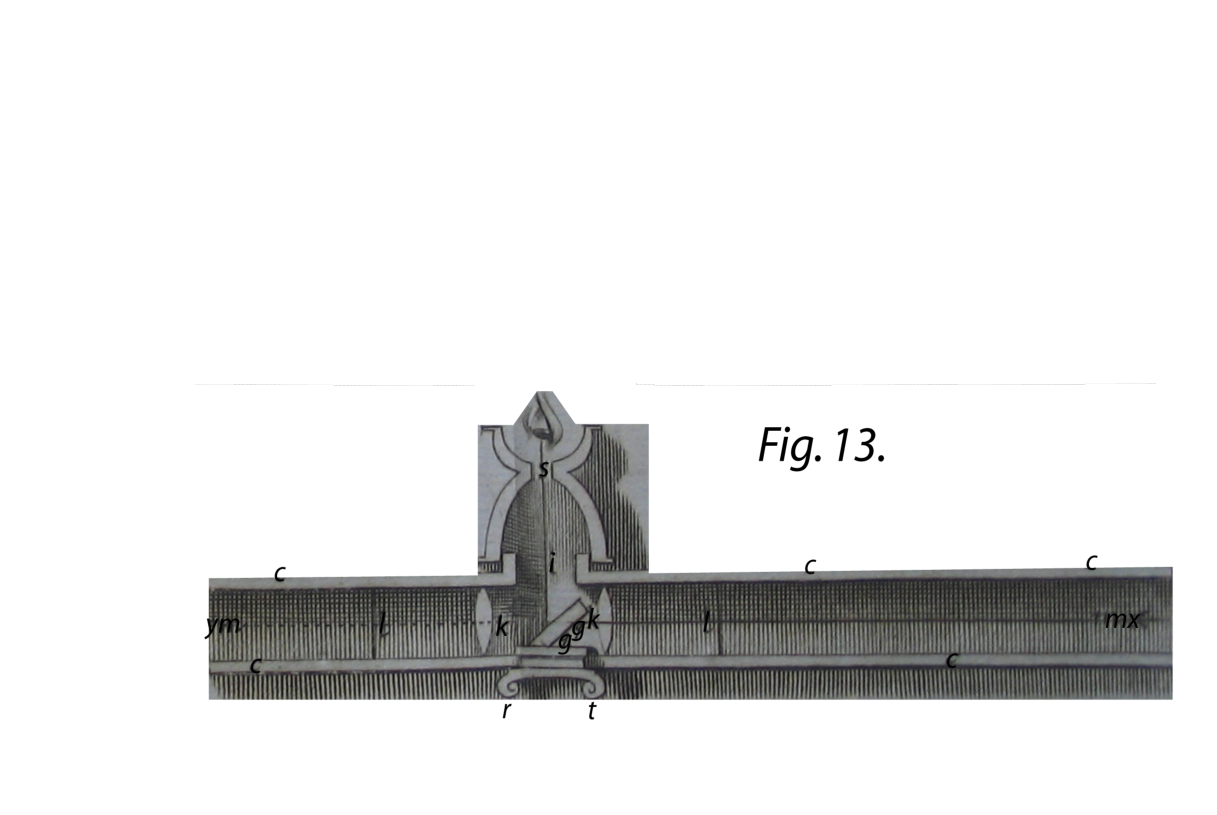
\includegraphics[trim = 0mm 0mm 0mm 1mm, clip, width=1\textwidth, angle=-0.5]{images/LH0351506_013r-dext13.pdf}\newline
\centering
[\textit{Fig. 4; erg. Hrsg. nach Hooke Fig. 13}]
\end{center}
\pstart\noindent Telescopica\protect\index{Sachverzeichnis}{telescopium}, et nisi perpendicularitas certa sit, omnis alius labor erit inutilis. \textso{Quoad primum} ut \edtext{fixentur fila dioptrica}{\lemma{fixentur}\Bfootnote{\textit{(1)} Dioptrae\protect\index{Sachverzeichnis}{dioptra} \textit{(2)} fila dioptrica \textit{L}}} utriusque Telescopii\protect\index{Sachverzeichnis}{telescopium} in eodem tubo, ita ut directe introrsum et retrorsum respiciant; cura adhibenda est, ut unum quodque ex quatuor vitris, hoc est duo vitra objectiva et duo ocularia\protect\index{Sachverzeichnis}{ocular}, ita firme et secure fixari possint in Tubo, ut nequeant \edtext{ulla vi}{\lemma{ulla}\Bfootnote{\textit{(1)} arte \textit{(2)} vi \textit{L}}} removeri ac disturbari. Sed hoc ita facile esse puto, ut non sit opus describere viam id praestandi. Secundo cura adhibenda, ne Tubi incurventur. Tertio unum ex filis dioptricis fixum esse debet ita ut vitra, et ita ut intersectio filorum ad crucem sit quoad ejus fieri potest in axe vitri objectivi et ocularis\protect\index{Sachverzeichnis}{ocular}; alterum filum dioptricum relinqui debet liberum donec multis experientiis inveniatur exacte in eadem linea cum priore, cujus rei praestandae modum nunc describam. Sint duo fila se ad angulos rectos secantia, unum perpendiculare alterum horizontale. Cura adhibenda, ut ambo jaceant exacte in eadem linea cum horizontali et perpendiculari \edtext{filis aliarum}{\lemma{}\Bfootnote{filis \textbar\ aliarum \textit{streicht Hrsg.} \textbar\ aliarum \textit{L}}} dioptrarum\protect\index{Sachverzeichnis}{dioptra}: et cum in finem sint \textit{two frames of brass,}\edtext{}{\lemma{\textit{brass},}\Cfootnote{a.a.O., S. 59.}} crassitie cavitatis Tubi habere ea opus est \edtext{\textit{groves}}{\lemma{\textit{groves}}\Cfootnote{a.a.O., S. 59.}} (gruben fossas) recipiendis ipsis aptas, in quibus ope cochlearum possint moveri \edtext{\textit{to and fro,}}{\lemma{\textit{to and fro},}\Cfootnote{a.a.O., S. 59.}} ut accommodentur. Postea opus est jungere ita exacte ut fila se tangere possint. Tertio opus est ut se exacte intersecent in foco vitrorum objectivi et ocularis\protect\index{Sachverzeichnis}{ocular}. \edtext{\textit{One of those frames}}{\lemma{\textit{frames}}\Cfootnote{a.a.O., S. 59.}} ducet filum perpendiculare, et ope cochleae in latere tubi mobile erit in latus dextrum aut sinistrum prout opus erit. \textit{The other frame}\edtext{}{\lemma{\textit{frame}}\Cfootnote{a.a.O., S. 59f.}} ducet filum horizontale, et ope cochleae in fastigio Tubi, fiet ita ut possit cadere et ascendere in Tubo, prout opus. His factis ex summitate turris vel alterius stationis \edtext{unde}{\lemma{}\Bfootnote{unde \textit{erg. L}}} duo opposita loca in distantia notabili v. g. \rule[-4mm]{0mm}{10mm}$\displaystyle\frac{1}{2}$ \edtext{\textit{mile, or a mile or two}}{\lemma{\textit{mile},}\Bfootnote{\textit{(1)} \textit{item one} \textit{(2)} \textit{or a mile or two} \textit{L}}}\edtext{}{\lemma{\textit{two},}\Cfootnote{a.a.O., S. 60.}} facile videri possint, inveni duo puncta quae primo inspectu per tua vitra invenis monstrari intersectione filorum dioptricorum, nota ea diligenter, ut certus sis red-inveniri \edtext{posse amotis vitris; quo facto circumage extremitates tubi}{\lemma{posse}\Bfootnote{\textit{(1)} \textbar\ amotis vitris \textit{erg.} \textbar\ quo facto circumage \textit{(2)} amotis \textit{(a)} Tubis \textit{(b)} vitris; quo facto circumage extremitates tubi \textit{L}}}, et (si ponas te introspexisse ab ortu versus occasum) inverte et partem orientalem fac esse occidentalem et contra, et inveni et duo eadem puncta rursus, inde dirigens partem quae habet fila fixa ad punctum ante visum dioptris mobilibus, quod certus es videre \textit{within the compas of your Eye-glass}\edtext{}{\lemma{\textit{Eye-glass}}\Cfootnote{a.a.O., S. 60.}} et observa quantum fila se secantia inde remota sint, versus
\pend
\newpage
\pstart 
%\begin{wrapfigure}{l}{0.5\textwidth}                    
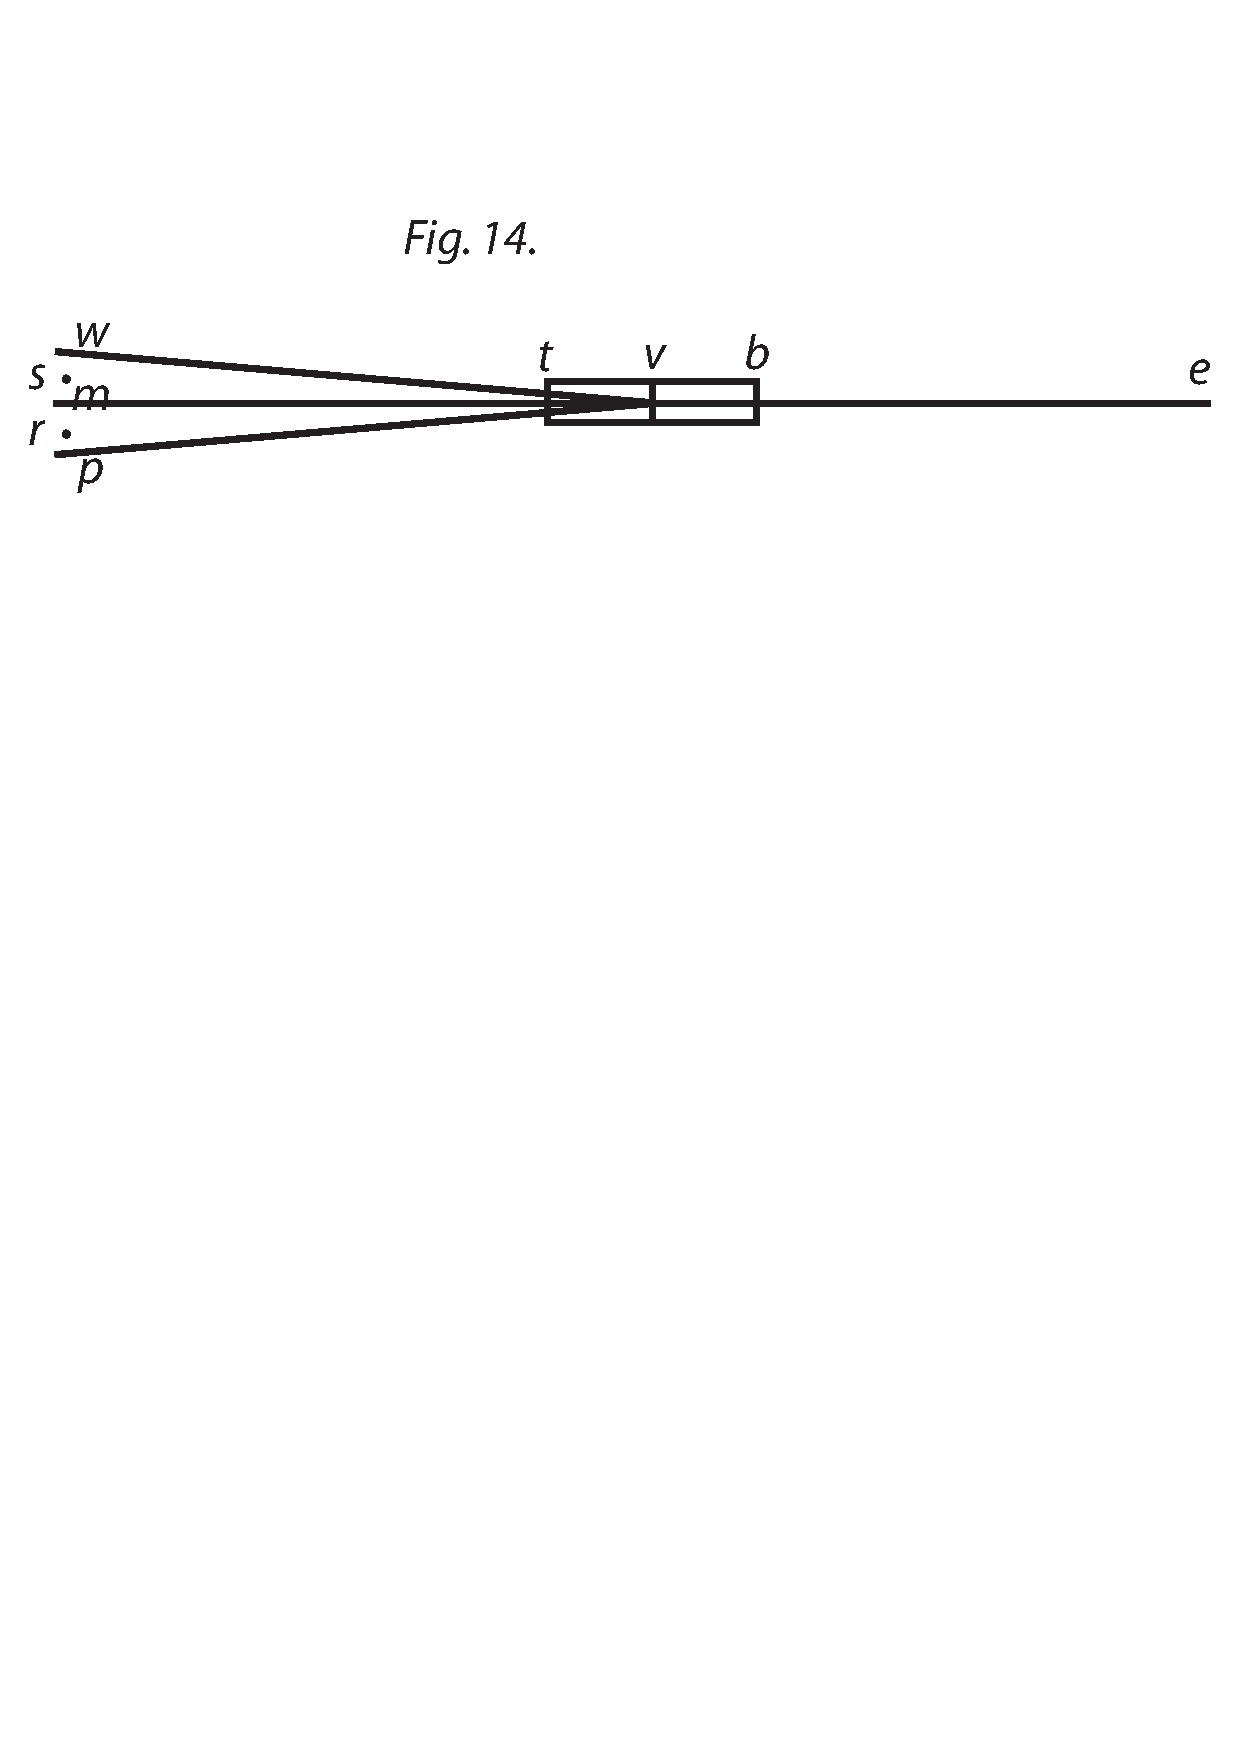
\includegraphics[trim = 0mm -5mm 0mm 0mm, clip,width=0.7\textwidth]{images/LH0351506_013r-dext14.pdf}\\
\centering \rule[0pt]{0mm}{0pt}[\textit{Fig. 5; erg. Hrsg. nach Hooke Fig. 14}]
%\end{wrapfigure}
\pend
\vspace{1em}
\pstart
\noindent \setline{1}Austrum vel Septentrionem sursum vel deorsum, inde quam prope potes, aestimatione hanc differentiam biseca et ope cochlearum \edtext{\textit{move the frames,}}{\lemma{\textit{move the frames,}}\Cfootnote{a.a.O., S. 60.}} ita ut fila sint in medio inter duo puncta: inde \edtext{rursus nota ea}{\lemma{rursus}\Bfootnote{\textit{(1)} observa ea \textit{(2)} nota ea \textit{L}}} puncta filis monstrata,
%\begin{wrapfigure}{l}{0.5\textwidth}                    
%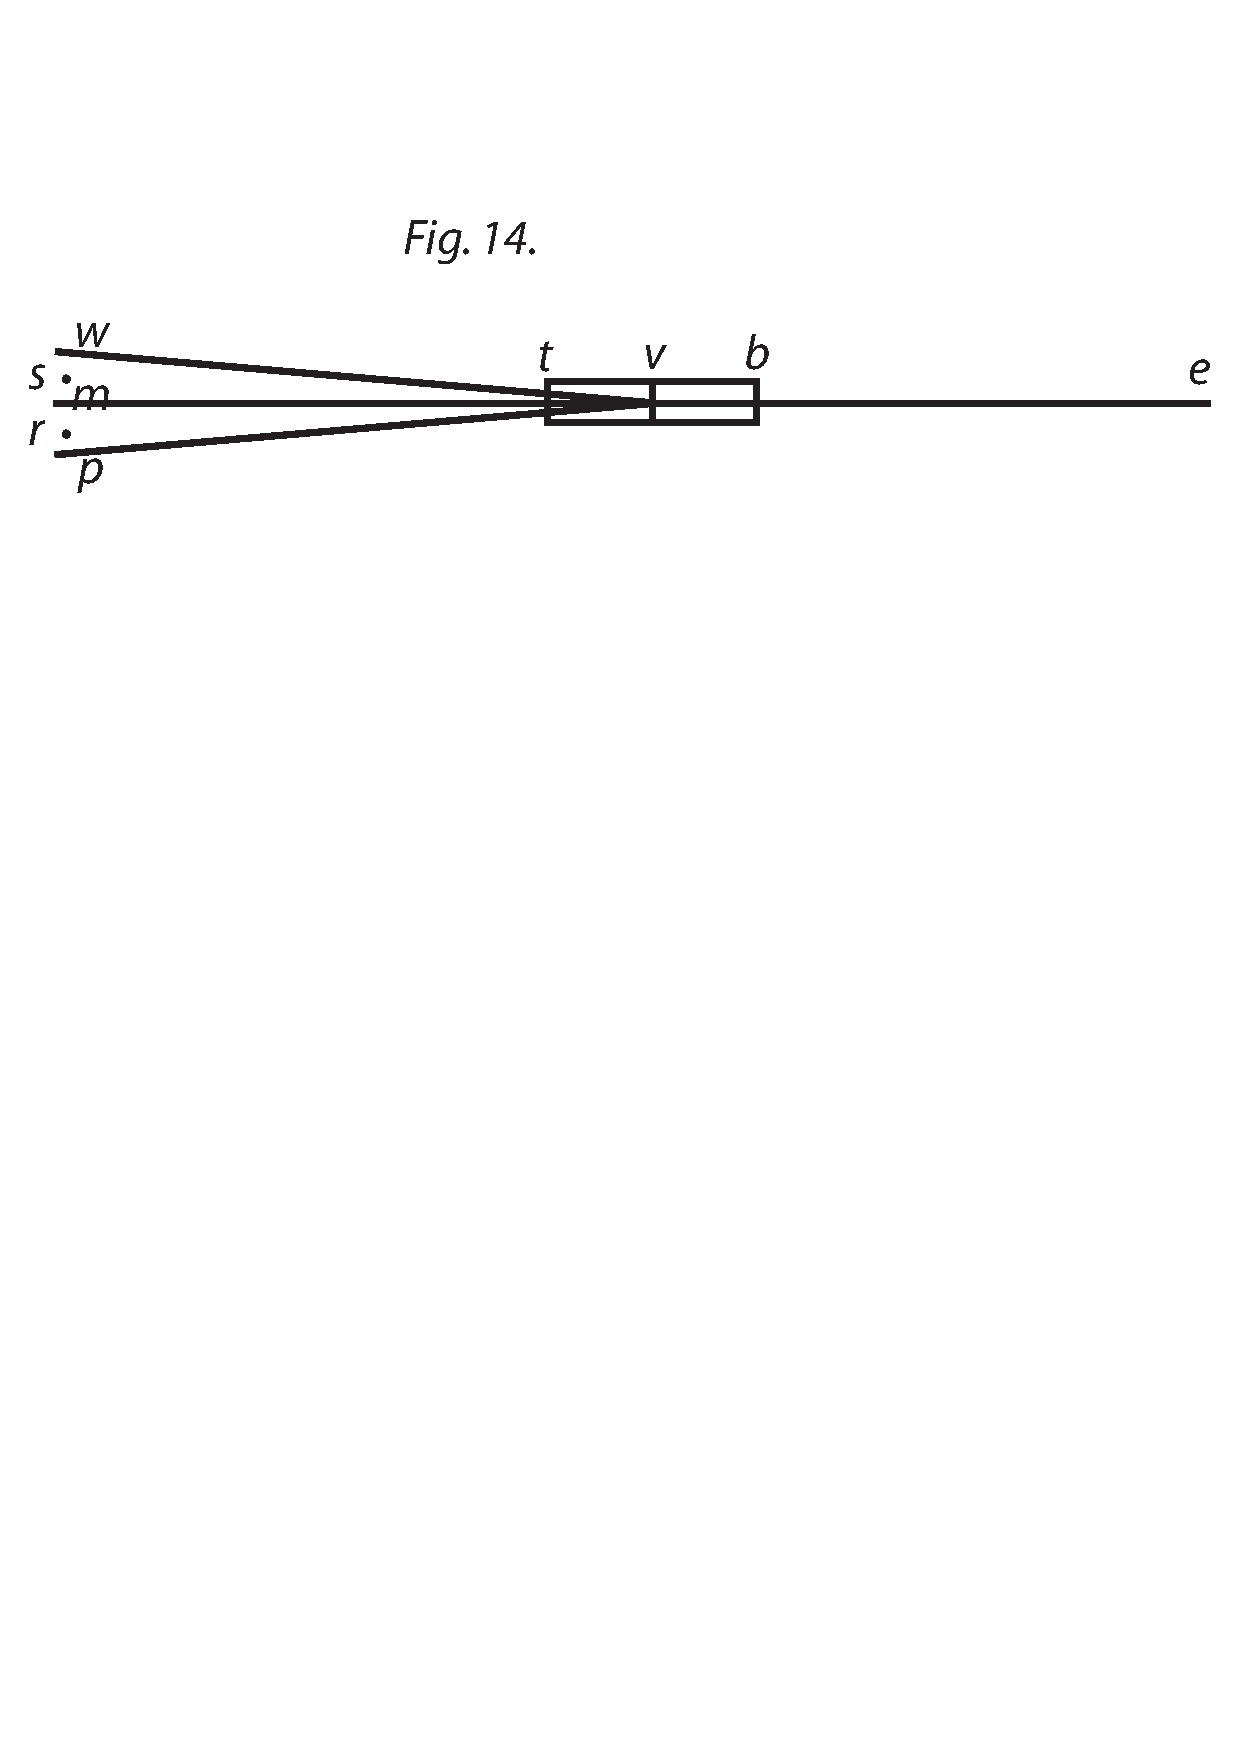
\includegraphics[width=0.5\textwidth]{images/LH0351506_013r-dext14.pdf}\\
%\rule[0pt]{3mm}{0pt}[\textit{Fig. 5; erg. Hrsg. nach Hooke Fig. 14}]
%\end{wrapfigure}
et [(]\textit{turn}\edtext{}{\lemma{\textit{turn}}\Cfootnote{a.a.O., S. 60.}}[)] circumage Tubum; hoc fac toties, donec circumacto tubo videas eadem puncta intersectionibus filorum notata, per quodcunque extremum introspicias, et hoc facto tubus erit exactus ad usum. Ratio hujus accommodationis plana illi qui inspexerit figuram 14. Pone enim \textit{v} repraesentare medium Tubi \textit{tvb} vel locum oculi, et \textit{w} repraesentare objectum visum occidentaliter, et \textit{e} objectum orientale, primo visu, inde servato exacte Tubi medio in eodem puncto \textit{u}, et circumagendo extremum Tubi \textit{t} versus orientem, et extremum \textit{b} versus occidentem et inveni primo objectum orientale \textit{e}; et inveniendo intersectionem nunc dirigere ad punctum \textit{p}, et non ad punctum \textit{w}. Divide distantiam inter puncta \textit{w} et \textit{p}, quam potes exacte in duas partes quod 
%    \hspace{-0.5mm}[13~v\textsuperscript{o}] si initio succedat exacte, erit medium punctum \textit{m}, sin rectifices solum usque ad \textit{r} et postea inverso tubo invenias \textit{s}, rursus rectificando ad medium differentiae inter \textit{r} et \textit{s}, et ita continuando, tertia aut quarta vice efficies, ut puncta \textit{m} et \textit{e} appareant in linea recta cum centro tubi duplicis. Hactenus de modo quo effici potest, ut diversa objecta utcunque integro semicirculo distantia simul videantur. \pend 
\count\Afootins=1200
\count\Bfootins=1200
\count\Cfootins=1200
\pstart \textso{Quarta pars} in qua quadrans noster excedit communis est exactitudo, qua altitudines sumi possunt, ope libellae aqueae \textit{water-level,}\edtext{}{\lemma{\textit{water-level,}}\Cfootnote{a.a.O., S. 61.}} ope cujus observator certus esse potest usque ad unum secundum aut duo. Ipsa libella est brevis tubus vitreus, longitudine 6 vel 8 pollicum, hermetice sigillatus utrobique, et repletus liquore qui neque congeletur, neque putrescat. Vitreus tubus sit quoad ejus fieri potest cylindricalis et rectus, quo propius recto, hoc exactius, dummodo habeat sensibilem curvaturam vel intumescentiam in medio; haec pars gibbosa erit superior, et tubus inclusus pyxidi cupreae\protect\index{Sachverzeichnis}{pyxis cuprea}. Vitrum \makebox[1.0\textwidth][s]{impleatur aqua distillata, cui circiter \rule[-2mm]{0pt}{9mm}$\displaystyle \frac{1}{3}$ bonae aquae fortis vel spiritus nitri affundatur,} 
\pend
\newpage
\pstart\noindent  ita neque putrescet, neque congelabitur. Fixetur in pyxide caemento duro. Et pyxis per cochleas firmabitur in latere quadrantis\protect\index{Sachverzeichnis}{quadrans} horizontali. 
\pend 
\pstart Brachio quadrantis\protect\index{Sachverzeichnis}{quadrans} immobili horizontaliter posito et limbo quadrantis\protect\index{Sachverzeichnis}{quadrans} sursum erecto, introspiciendo in centro observa dua objecta horizontalia, seu in horizonte posita, et sibi invicem opposita: observa limites bullae aereae in summitate liquoris in quolibet latere medii libellae, et fac notam, inde circumactis quadrantis\protect\index{Sachverzeichnis}{quadrans} extremis, pone donec extrema bullae stent ut in priore observatione inde rursus aspice eadem objecta in horizonte posita, et invenies differentiam inter priorem et hanc observationem; hanc biseca qua potes exactitudine, et aestimatione oculi pone dioptras\protect\index{Sachverzeichnis}{dioptra} in medio eorum inclinando quadrantem\protect\index{Sachverzeichnis}{quadrans}, inde per cochleam ita \edtext{rectifica libellam}{\lemma{rectifica}\Bfootnote{\textit{(1)}\ Tubum \textit{(2)}\ libellam, \textit{L}}}, ut extremum bullae aequaliter a medio distet, et rursus converte quadrantem\protect\index{Sachverzeichnis}{quadrans}, et vide an extremis bullae eodem loco stantibus duae oppositae dioptrae\protect\index{Sachverzeichnis}{dioptra} \edtext{telescopicae\protect\index{Sachverzeichnis}{telescopium} eadem objecta respiciant}{\lemma{telescopicae}\Bfootnote{\textit{(1)}\ videant \textit{(2)}\ eadem objecta respiciant; \textit{L}}}; quo posito certus eris perfectae horizontalitatis dioptrarum\protect\index{Sachverzeichnis}{dioptra} in fixo quadrantis\protect\index{Sachverzeichnis}{quadrans} brachio; sin minus tamdiu repetes examen donec succedat. Sed cum hoc genus perpendicularis subjectum sit incommoditati caloris et frigoris, quod rarefacit et condensat aeris bullam, et proinde facit bullam aeris minorem aut majorem; cura adhibenda est, ut varietates quae in ea producuntur per gradus caloris et frigoris, notentur. Quod ita facile efficies: Tubum ope glaciei et salis reduc ad quantum potes gradum frigoris; inde methodo proxime explicata, pone quadrantem\protect\index{Sachverzeichnis}{quadrans} horizontalem, et nota extrema bullae per 4.4. Inde paulatim aerem rarefac, et rursus observa expansionem et nota haec in vitro ope diamantis 3.3. vel 2.2. vel 1.1. vel 0.0. quo facto facillimum erit quovis tempore accommodare quadrantem\protect\index{Sachverzeichnis}{quadrans} ad exactitudinem desideratam cum appareant extensionis gradus; \textit{by being carefull to see, that the two ends of the bubble be proportionably extended, as to 00. 11. 22. 33. 44. etc. or to any intermediate space.}\edtext{}{\lemma{\textit{space}.}\Cfootnote{a.a.O., S. 62.}} Ratio exactitudinis haec est, quod superior pars \edtext{Tubi propinqua}{\lemma{Tubi}\Bfootnote{\textit{(1)}\ propior \textit{(2)}\ propinqua \textit{L}}} rectae lineae, ac proinde vel pars circuli ex ingenti radio vel quaedam curva irregularis circulo valde propinqua. Quantum ad hoc libellandi negotium, et ideo gradus \edtext{talis circuli proportionaliter}{\lemma{gradus}\Bfootnote{\textit{(1)}\ ejus pro \textit{(2)}\ talis circuli proportionaliter \textit{L}}} \edtext{erit magnus}{\lemma{erit}\Bfootnote{\textit{(1)}\ longus \textit{(2)}\ magnus, \textit{L}}}, et flexura tubi fieri potest ex curva radii tam magni, ut quaelibet secunda inclinationis producat in libella mutationem longitudinis valde sensibilis. Hoc difficulter efficietur communi via perpendiculorum seu plumborum suspensorum, nisi ex maxima pendeant altitudine, quod nec facile effici potest in praxi sine multa difficultate, et si obtineatur, nullius potest esse usus, ob magnitudinem apparatus, necessarii ad superan-
\pend
\newpage
\pstart\noindent dam structurae incertitudinem, et motum aeris, aliaque. Jam curvatura hujusmodi potest esse portio sphaerae radii 1000 pedum et ultra; et ideo minutum ejus non erit minus quam \rule[-5mm]{0pt}{12mm}$\displaystyle \frac{29}{100}$ pedis, et secundum minutum erit \textit{almost}\edtext{}{\lemma{\textit{almost}}\Cfootnote{a.a.O., S. 63.}} semicentesima pedis, quod sufficienter distingui potest nudo visu. Si cylinder vitreus sit 9 pollicum continebit duo minuta ejusmodi circuli, inter \textit{f} et \textit{f}. et unum inter 4 et 4. et ideo horizontalitas vitri hujus haberi potest ad certitudinem usque minuti secundi, quod vix alia ratione fieri potest. Sed restat difficultas ingens quomodo ejusmodi curvatura fieri possit, cum raro tubi vitrei reperiantur curvati, ut desiderari potest, et hoc tam est difficile quam invenire eos plane rectos. Hoc ut praeveniatur si adhibendae cannae vitreae, cura adhibenda, et varia tentamenta facienda, ut inveniatur quae vitra, et quae latera apta. Nam nostri vitri flatores non habent modum ea certo faciendi, curvaturae aut rectitudinis desideratae nec facile postea a tornatore eam accipiunt. Sed diligentia et tentamenta facile invenient ex multis in officina vitraria factis, aliqua. Ego uno usus sum alterius \edtext{formae \textit{25. fig., wich}}{\lemma{formae}\Bfootnote{\textbar\ \textit{25. fig.} \textit{erg.} \textbar\ , \textit{(1)}\ qui \textit{(2)}\ \textit{wich} \textit{L}}} \textit{i found to do, exceeding \edlabel{hooke3}well}\edtext{}{\lemma{\textit{well}}\Cfootnote{a.a.O., S. 64.}}\edtext{}{{\xxref{hooke3}{hooke4}}\lemma{\textit{well}}\Bfootnote{\textit{(1)}\ nigra parte aquam, lucida aerem repraesenta \textit{(2)}\ . Factus \textit{L}}}. Factus\edlabel{hooke4} erat is tubus ex duobus vitris \textit{drawn in distinct pipes at the glass-house but joyn'd together in the Lamp,}\edtext{}{\lemma{\textit{Lamp},}\Cfootnote{a.a.O., S. 64.}} et superior pars largioris vel inferioris Tubi, erat incurvata deorsum convexitate sua, ita ut aqua tangeret mediam partem, et bullae aeris extremo utriusque communicarent \edtext{invicem \textit{by the small pipe above}}{\lemma{invicem}\Bfootnote{\textit{(1)}\ per superiorem exiguam \textit{(2)}\ \textit{by the small pipe above.} \textit{L}}}\edtext{}{\lemma{\textit{above}.}\Cfootnote{a.a.O., S. 63.}}. Aliam etiam rationem expertus sum
%\begin{wrapfigure}{l}{0.4\textwidth}                    
%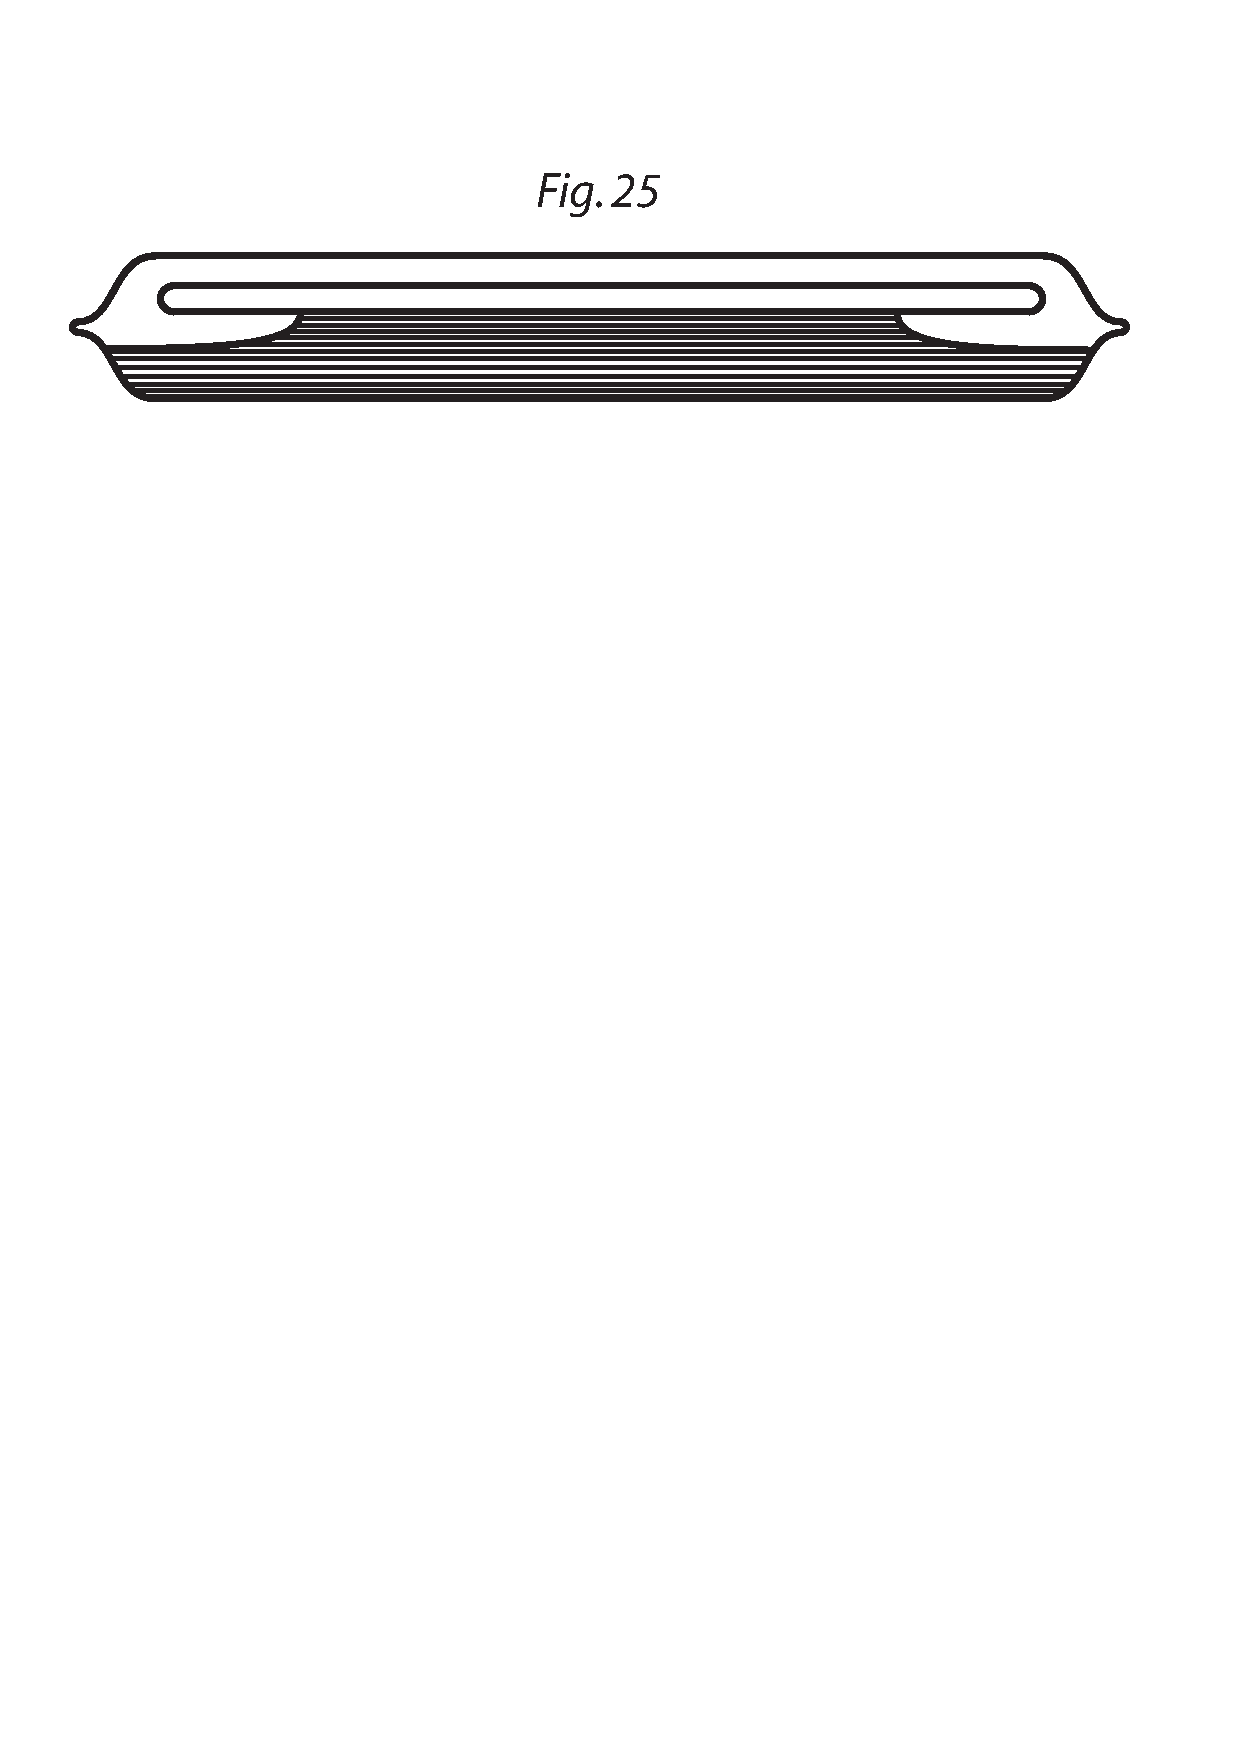
\includegraphics[width=0.4\textwidth]{images/LH0351506_013v-d1.pdf}\\
%\rule[0pt]{5mm}{0pt}[\textit{Fig. 6, nach Hooke Fig. 25}]
%\end{wrapfigure}
cujus ope certior fui curvitatis, et eam habui ex circulo majore. Hoc erat ope longi frusti speculi (\textit{looking glass plate}\edtext{}{\lemma{\textit{plate}}\Cfootnote{a.a.O., S. 64.}}) positi admodum quod ope [14~r\textsuperscript{o}]\edtext{}{\lemma{}\Afootnote{\textit{Oberhalb des Textes}: Pars III. Excerptorum ex Hookio contra Hevelium\vspace{-5mm}}} cochlearum\hfill tendebam\hfill (\textit{wich\hfill by\hfill the\hfill help\hfill of\hfill Screws\hfill i\hfill bent)\hfill upon\hfill the\hfill circular\hfill edges\hfill of\hfill a} 
\pend
%\vspace{0.5em}
\pstart
%\setline{26}
\noindent
\centering
%\begin{wrapfigure}{l}{0.4\textwidth}                    
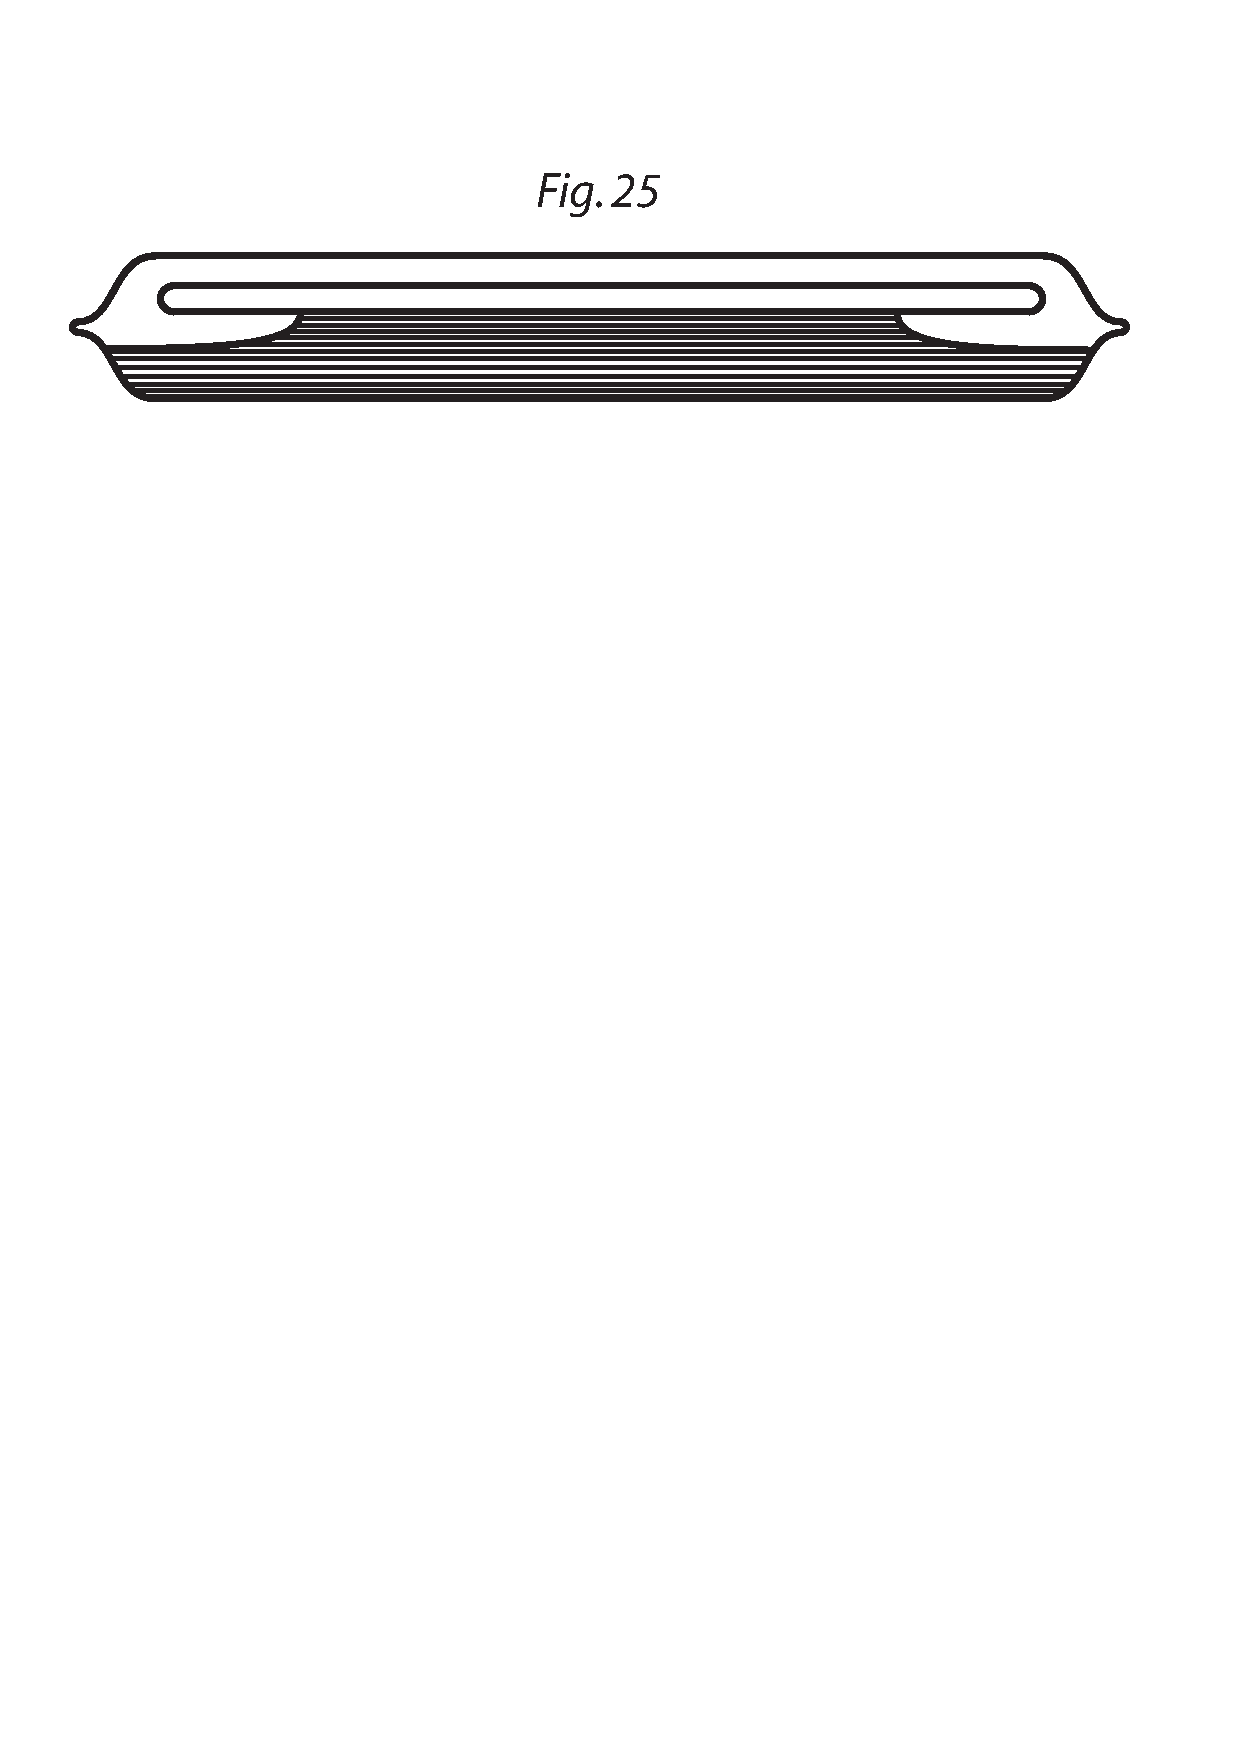
\includegraphics[width=0.6\textwidth]{images/LH0351506_013v-d1.pdf}\\
\centering \rule[0pt]{6mm}{0pt}[\textit{Fig. 6, nach Hooke Fig. 25}]
%\end{wrapfigure}
\pend 
\newpage
\pstart
%    \noindent \textit{brass prismatical-box,}\edtext{}{\lemma{\textit{prismatical-box},}\Cfootnote{a.a.O., S. 64.}} et eam cementabam \textit{very tight, with hard and soft Ciment}\edtext{}{\lemma{\textit{Ciment}}\Cfootnote{a.a.O., S. 64.}}. Habebat \textit{the plate}\edtext{}{\lemma{\textit{plate}}\Cfootnote{a.a.O., S. 64.}} (frustum, lamina) curvum canalem, \textit{ground in it in the length thereof}\edtext{}{\lemma{\textit{thereof}}\Cfootnote{a.a.O., S. 64.}} aptum ad servandam in medio bullam. Horum mediorum ope non est difficile tendere seu curvare hanc laminam seu tabulam in circulum 50, 60, 100, 1000 pedum radiorum, \textit{and the Brass Box can easily be made to fill or empty, as there shall be occasion for the use thereof, so that the bubble may be at any time left, of what bigness shall be desired. It will be convenient also, to varnish the inside of this brass-box, with laker-varnish, very thik and close, }\edtext{\textit{both to keep it from}}{\lemma{\textit{close},}\Bfootnote{\textit{(1)}\ tum ut \textit{(2)}\ \textit{both to keep it from} \textit{L}}} \textit{rusting, and also to preserve it from being corroded by Aqua fortis, whensoever there shall be occasion to put it in for the cleansing the inward tarnish and foulness of the Glass-Plate.}\edtext{}{\lemma{\textit{Glass-Plate}.}\Cfootnote{a.a.O., S. 65.}} Curvitas \edtext{superioris lateris}{\lemma{superioris}\Bfootnote{\textit{(1)}\ partis \textit{(2)}\ lateris \textit{L}}} libellae potest fieri, \textit{by grinding}\edtext{}{\lemma{\textit{grinding}}\Cfootnote{a.a.O., S. 65.}} inferius latus \textit{of such a long plate of looking glass, upon a convex glass-tool, of 50, 60, 100, 1000, foot radius et polishing the same, accordingly of that figure.}
\pend
\vspace{3.5em}
\pstart
%\noindent
\count\Afootins=1200
\count\Bfootins=1200
\count\Cfootins=1200 
%\begin{center}
\centering 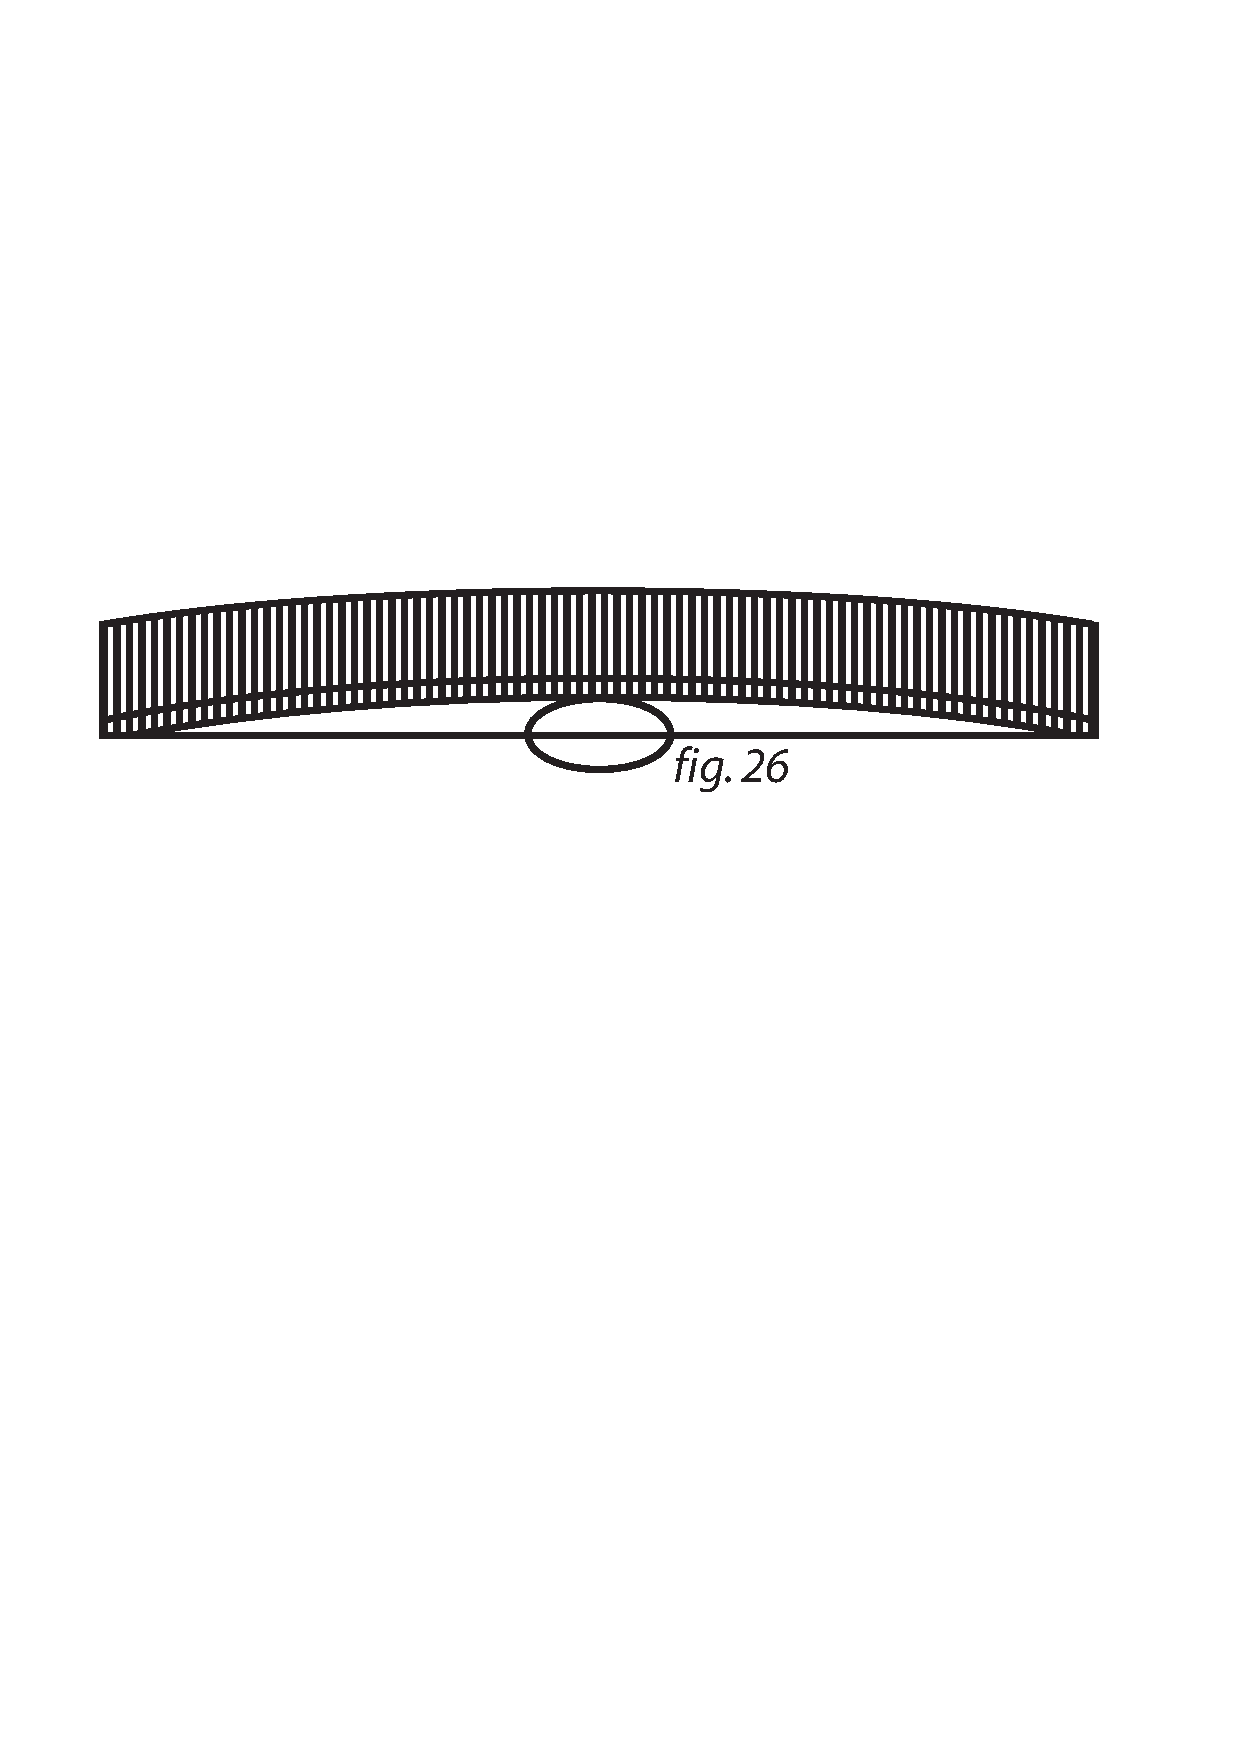
\includegraphics[trim = 0mm -1mm 0mm 0mm, clip, width=0.6\textwidth]{images/LH0351506_014r-d1.pdf}\\
\centering [\textit{Fig. 7, nach Hooke Fig. 26}]
\pend
\vspace{2.5em}
\setline{16}
\pstart
%\noindent
\centering
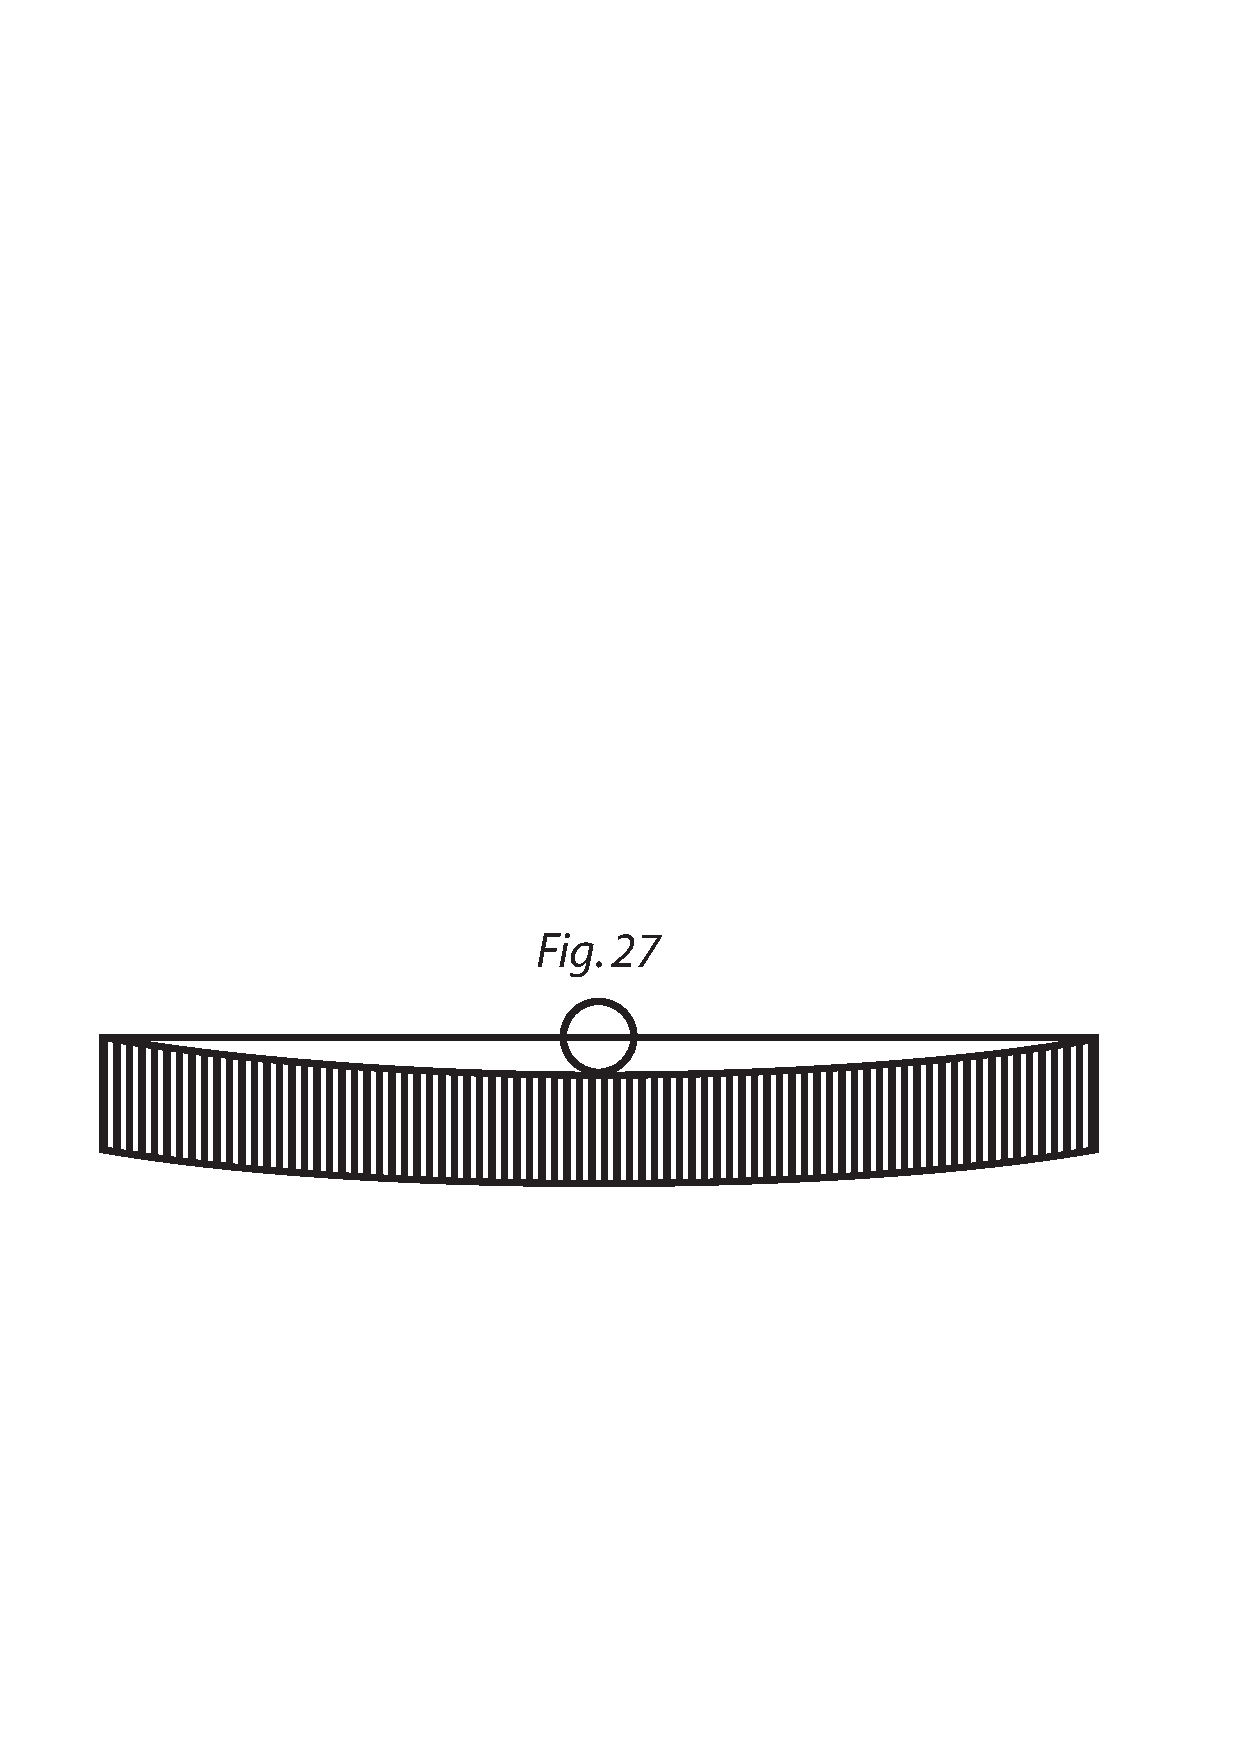
\includegraphics[trim = 0mm -4mm 0mm 0mm, clip, width=0.6\textwidth]{images/LH0351506_014r-dext27.pdf}\\
\centering [\textit{Fig. 8, erg. Hrsg. nach Hooke Fig. 27}]
%\end{center}
\pend
%\vspace{1em}
\newpage
\pstart \textit{The curvity of the said plate is express'd 26 fig.}\edtext{}{\lemma{\textit{fig}.}\Cfootnote{a.a.O., S. 65.}} Jam quicquid hac via fieri potest aqua et bullis aeris idem fieri potest \textit{with the same glasses turned upside-down,}\edtext{}{\lemma{\textit{upside-down},}\Cfootnote{a.a.O., S. 65.}} ope exacte rotundi et politi cylindri vel globuli vitrei, vel ex crystallo, \textit{cornelian, Agate,}\edtext{}{\lemma{\textit{Agate},}\Cfootnote{a.a.O., S. 65.}} aut alio lapide \textit{exceeding hard and close}\edtext{}{\lemma{\textit{close}}\Cfootnote{a.a.O., S. 65.}}. Modo in 27 figura repraesentato, quae est inversa tantum fig. 26\textsuperscript{tae}. Quod enim illic bulla aeris quae summum petit, id hic facit globus qui tendit ad imum, sed opus est tum ut globulus sit valde rotundus, tum ut concavitas tabulae sit exacte polita ac libera ab omni pulvere, alioquin posset fieri ut globulus vel cylinder in debito loco quiesceret. Non possum hic quin mentionem faciam curiosae admodum libellae a Christophoro Wrenno\protect\index{Namensregister}{\textso{Wren}, Christopher (1632-1723)} \edtext{inventae}{\lemma{inventae}\Cfootnote{Vgl. \textsc{R. Hooke} (a.a.O., S. 65), der von solch einem Instrument Wrens berichtet.}} pro sumendo horizonte \textit{every way in a Circle.}\edtext{}{\lemma{\textit{Circle}.}\Cfootnote{a.a.O., S. 65.}} Quod fit largo concavo tornato ac polito ex sphaera valde larga, \textit{and the limb of it ground and polisht on} \edtext{\textit{a flat}}{\lemma{\textit{on}}\Bfootnote{\textit{(1)}\ \textit{a very large sphere} \textit{(2)}\ \textit{a flat} \textit{L}}}\textit{, for}\edtext{}{\lemma{\textit{for}}\Cfootnote{a.a.O., S. 65.}} \edtext{nam horizontaliter locando}{\lemma{\textit{for}}\Bfootnote{\textit{(1)}\ \textit{by placing} \textit{(2)}\ nam horizontaliter locando \textit{L}}}, et exiguam Hydrargyri guttulam infundendo, facile erit ope hujus limbi politi verum horizontem detegere. Unam ego inconvenientiam reperio, quod Mercurius habet aliquod genus adhaesionis ad vitrum, sed exiguus globulus crystallinus malo mederi potest. 
\pend 
\pstart Quinta instrumenti excellentia est, quod summae illae inconvenientiae in movendo instrumento una cum objecto possunt evitari; instrumento objectum sua sponte sequente. \textit{I make an axis of very dry and strong dram-fir}\edtext{}{\lemma{\textit{dram-fir}}\Cfootnote{a.a.O., S. 67.}} \edtext{magnae satis crassitiei}{\lemma{\textit{dram-fir}}\Bfootnote{\textit{(1)}\ \textit{of a bigness} dig \textit{(2)}\ magnae satis crassitiei \textit{L}}} pro longitudine ne curvetur in inferiore ejus parte, figo in medio \edtext{[\textit{well bound and hoop'd about} (hoope, vieo, binder) \textit{with iron}]}{\lemma{[\textit{well ... iron}]}\Cfootnote{a.a.O., S. 67, eckige Klammern von Leibniz.}} centrum vel punctum chalybeum, valde bene tornatum duratum et acutum, quod moveatur in foramine conico apto ad ipsum recipiendum, etiam ex bono et durato chalybe: et ab altero latere hujus arboris vel virgae figo aliam chalybeam portionem in ipso medio, quod qua parte ligno immediate contiguum est, habet \textit{a Neck very well tourned and hardned, a little tapering from the wood outward, wich is to be moved in a collar fit for it, as i shal shew by and by, and at a convenient distance from the said neck, as at somewhat more then half the radius of the instrument, is made a cylindrical-neck, fitted with a collar of brass with a joynt and other apparatus, large enoug to carry the Table and Instrument firm and true, without sliding or yielding in its socket after it be once set. This axis by the collar and conical hole below, i place parallel to the axis, wich by some tryals is easely enoug adjusted; about the cylindrical Neck, at the upper end of this Axis, is a Socket of Brass, fastned with a screw, wich Socket claspeth in a joynt, a short arm, wich has at one end a Ball that is fitted into a socket,}
%\edtext{}{\lemma{socket,}\Cfootnote{a.a.O., S. 67.}} 
%    \hspace{-0.7mm}[14~v\textsuperscript{o}] \textit{that is fixed unter the table and frame of the quadrant\protect\index{Sachverzeichnis}{quadrans}, and of the other end a counterpoise of lead, tho ballance the weight of the whole apparatus, about the Quadrant\protect\index{Sachverzeichnis}{quadrans} upon the middle line, of the long Axis, then the Table and Quadrant\protect\index{Sachverzeichnis}{quadrans} is rectifi'd, so as to lye in the plain of the two celestial objects, whether planets or fixt stars, and by the small screws in the sockets, it is fixt in that plain.}\edtext{}{\lemma{\textit{plain}.}\Cfootnote{a.a.O., S. 67.}} Alia requisita \edtext{adaptationis}{\lemma{}\Bfootnote{adaptationis \textit{erg. L}}} facile fiunt ope exiguarum cochlearum in quadrante\protect\index{Sachverzeichnis}{quadrans} ipso. Tabula accommodata plano objectorum cum quadrante\protect\index{Sachverzeichnis}{quadrans} \textit{on it,}\edtext{}{\lemma{\textit{on it,}}\Cfootnote{a.a.O., S. 67.}} et omnibus exacte satis aequilibratis ope ponderum sub Tabula, et fixis dioptris, ad unum dictorum objectorum directis, dicta tabula et instrumentum continuant in eodem plano manere sine ulla alia incommoditate observatoris quanquam objecta semper mutent locum; et fixa dioptra\protect\index{Sachverzeichnis}{dioptra} manet directa ad objectum \edtext{unum}{\lemma{}\Bfootnote{unum \textit{erg. L}}} donec ope mobilis quaeratur objectum alterum. Quod ut efficiatur motu Tabulae et instrumenti; Horologium adaptatum est axi, quod eodem tempore ipsum revolvi faciat quo terra absolvit motionem diurnam, et ita sequetur semper motum apparentem stellarum fixarum quod ita fiet: circa partes quasdam Axis, ubi locus videbitur commodissimus fixetur octava pars rotae radii tripedalis, ejus \textit{Rim}\edtext{}{\lemma{\textit{Rim}}\Cfootnote{a.a.O., S. 68.}} (margo puto) exacte tornetur, et acies ejus secetur in dentes 360. tot enim sunt dimidia horae minuta, in octava parte integrae revolutionis, quanquam haec minuta \edtext{[halve]}{\lemma{}\Bfootnote{harve \textit{L \"{a}ndert Hrsg.}}} horae, quae respiciunt fixas, notabiliter breviores erunt quam solares. \textit{Then fit a worm or screw}\edtext{}{\lemma{\textit{screw}}\Cfootnote{a.a.O., S. 68.}} at \edtext{[hos]}{\lemma{}\Bfootnote{has \textit{ L \"{a}ndert Hrsg.}}} dentes, ita ut una \edtext{revolutione cochleae}{\lemma{revolutione}\Bfootnote{\textit{(1)}\ spirae \textit{(2)}\ cochleae \textit{L}}} facta in semiminuto, faciat \edtext{[unum]}{\lemma{}\Bfootnote{unam \textit{L \"{a}ndert Hrsg.}}} dentem moveri prorsum, \textit{the revolution of the worm is adjusted by a circular pendulum, wich is carried round by a flie}\edtext{}{\lemma{}\Afootnote{\textit{Oberhalb a flie}: un volant \Denarius\vspace{-6mm}}}\textit{, moved in the form of a one wheel'd jack from a swash toothed wheel,} \edtext{\textit{fastned upon}}{\lemma{\textit{fastned}}\Bfootnote{\textit{(1)}\ \textit{about} \textit{(2)}\ \textit{upon} \textit{L}}} \textit{the shank of the worm or screw above mentionn'd; the weight that carries round this wheel must hang, upon the shank of the worm, and must be about a 3}\textsuperscript{\textit{d}} \textit{or 4}\textsuperscript{\textit{th}} \textit{part of the weight of the quadrant\protect\index{Sachverzeichnis}{quadrans} and Table, that it may carry it round steadily and strongly and the circular pendulum must be so order'd, that the observator may at any time of his observation either shorten or produce the length thereof, so as to make it}
\pend
\newpage
\pstart\noindent \textit{move quicker or slower,}\edtext{}{\lemma{\textit{slower},}\Cfootnote{a.a.O., S. 68.}} pro ut res postulabit, quod fiet, \textit{by sliding the hole upon wich the pendulum makes its conical motion a little higher or lower, without lifting up or letting down the pendulum}\edtext{}{\lemma{\textit{pendulum}}\Cfootnote{a.a.O., S. 68.}} (exaltando aut demittendo cavitatem conicam pondere pendulo non ascendente vel descendente) vel etiam penduli filo nonnihil attracto uffgewunden, vel demisso, ope cylindri circa foramen aut apicem coni in quo movetur pendulum. De modo construendi pendulum circulare nihil amplius dico, et id alteri tempori servo, cum quibusdam aliis circa motum experimentis, quae mihi inveniendi ejus occasio fuere, anno 1665. Qua occasione non possum quin loquor de libro ab Hugenio\protect\index{Namensregister}{\textso {Huygens}, Christiaan (1629-1695)} edito, ubi etiam brevem exhibet descriptionem ejusmodi penduli circularis, me non nominato,\edtext{}{\lemma{nominato,}\Cfootnote{\textsc{C. Huygens}, \textit{Horologium oscillatorium}, Paris 1673, S. 159f.\cite{00123} (\textit{HO} XVIII, S. 360-365). Das erste Projekt einer Uhr mit einem Kreispendel stammt aus dem Jahr 1659. Vgl. dazu: \textit{Projet de 1659 d'une horologe \`{a} pendule conique}, \textit{HO} XVII, S. 85-91.}} perinde ac nihil ea res ad me pertineret, quanquam jam anno 1665. invenerim et in usum transtulerim; communicavi societati regiae ejus tam theoriam quam praxin, et speciatim explicabam isochronam motionem pilae penduli, in superficie parabolica, una cum modo Geometrico et mechanico, efficiendi ut in tali superficie moveatur. Hujus rei testes habeo societatis Regesta,\edtext{}{\lemma{Regesta,}\Cfootnote{\textsc{T. Birch}, \textit{History}, London 1757, Bd.~I, S. 97 und 108\cite{00154}; hier sind Hookes Untersuchungen zum Kreispendel f\"{u}r das Jahr 1666 festgehalten.}} et Morayus\protect\index{Namensregister}{\textso {Moray}, Robert (1608-1673)} dixit se Hugenio\protect\index{Namensregister}{\textso {Huygens}, Christiaan (1629-1695)} scripsisse sed de eo plura postea; (alio tractatu) quando examinabo alia in eo libro contenta, circa descensum corporum gravium inveniendum, et circa inventionem longitudinis locorum, productis aliis rationibus certioribus et practicabilioribus. Haec faciunt 
%    [15r\textsuperscript{o}] ut hoc loco publicare velim inventum meum, cujus ope res omnis rotas concernens ad summam promoveri possit perfectionem, quod et produxi anno 1666, cum fundetur in principio capace summae perfectionis imaginabilis. Id breviter eo redit ut efficiatur compositum ex rotis dentatis, ita ut habeatur numerus dentium quantumvis, nec tamen ideo illi exigui nimis ac debiles reddantur; deinde ut motio aequaliter communicetur a rota in rotulam (+ pignon +). Tertio ut punctum contactus et sustentationis, \textit{of touching and bearing,}\edtext{}{\lemma{\textit{bearing},}\Cfootnote{a.a.O., S. 70.}} sit semper in linea duo centra jungente; \textso{quarto} ut nulla sit defrictio sive detritio: denique omnia non sunt elaborata difficiliora quam communia, excepto quod opifex his nondum assuetus. Itaque primo, si sit certus numerus requisitus dentium, 
%\begin{wrapfigure}{l}{0.5\textwidth}                    
%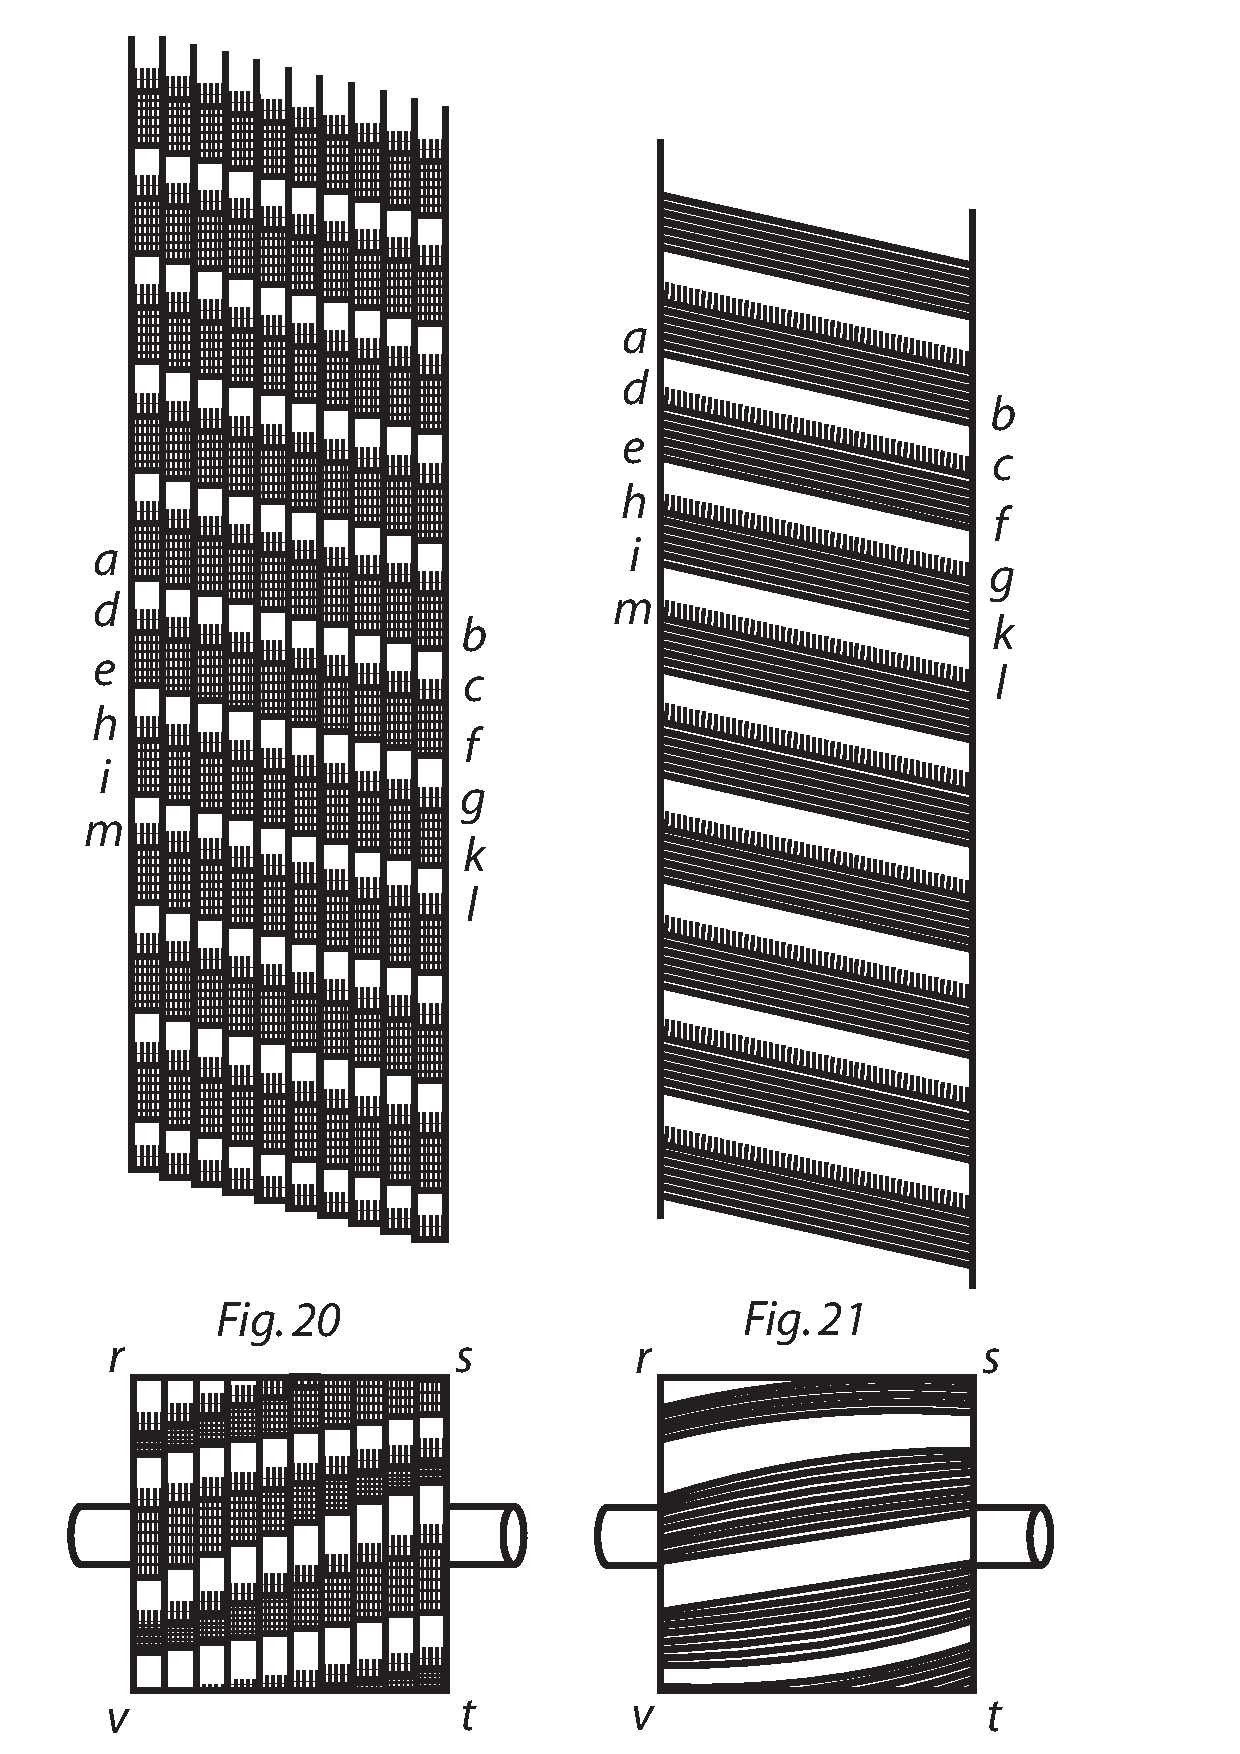
\includegraphics[width=0.5\textwidth]{images/LH0351506_014-dext20u22.pdf}\\
%\rule[0pt]{0mm}{0pt}[\textit{Fig. 9, erg. Hrsg. nach Hooke Fig. 20 u. 21}]
%\end{wrapfigure}
et non ultra requisitus faciendae exiguae rotae, necesse est, ut rotae et rotulae constent ex compluribus laminis vel rotis quae jaceant aliae apud alias, ratione quae apparet in figura 20\textsuperscript{ma}. Ibi suppone requiri ut rota habeat dentes 1000, et pignon 100, 
et dentes pariter Rotae et Rotulae (pignon) habere fortitudinem sufficientem;
\pend
\newpage
\pstart \noindent 
\begin{wrapfigure}[27]{l}{0.52\textwidth}    
\vspace{-6mm}                
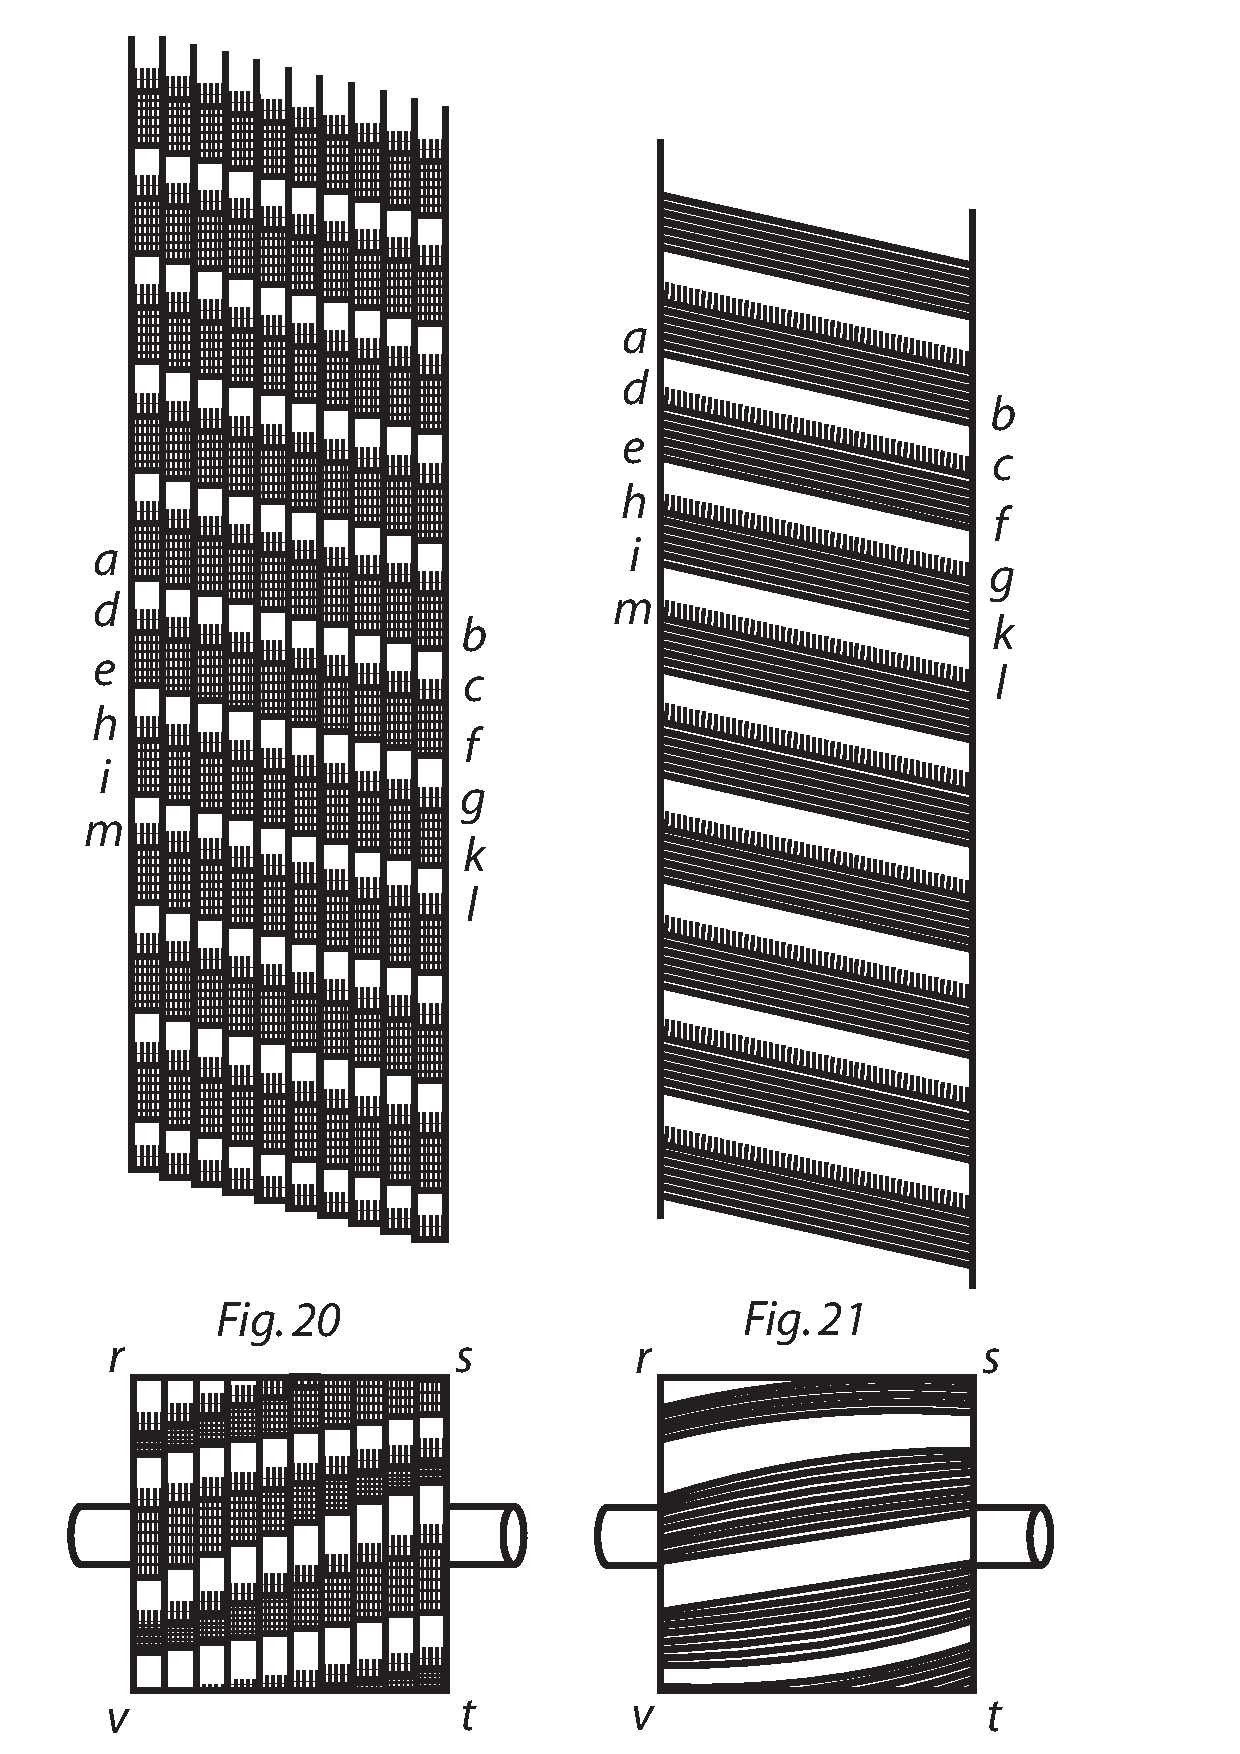
\includegraphics[trim = 0mm -2mm -5mm 0mm, clip, width=0.52\textwidth]{images/LH0351506_014-dext20u22.pdf}\\
\rule[0pt]{0mm}{0pt}[\textit{Fig. 9, erg. Hrsg. nach Hooke Fig. 20 u. 21}]
\end{wrapfigure}
sume \textit{10 Plates}\edtext{}{\lemma{\textit{10 Plates}}\Cfootnote{a.a.O., S. 71.}} (laminas) omnes ejusdem crassitiei, et ope duarum pluriumve \edtext{cochlearum firma atque contine}{\lemma{cochlearum}\Bfootnote{\textit{(1)}\ fixa \textit{(2)}\ sicut \textit{(3)}\ atque \textit{(4)}\ firma atque contine \textit{ L}}}, quasi \edtext{unam rotam;}{\lemma{}\Bfootnote{unam \textbar\ facere \textit{ gestr.}\ \textbar\ rotam; \textit{ L}}} hanc rotam seca in 100 dentes et comple; inde mediam (inter has laminas) cavitatem adapta rotundo arboris (: \textit{upon the round neck of an arbor}\edtext{}{\lemma{\textit{arbor}}\Cfootnote{a.a.O., S. 71.}} :) inde cochleam laxa, libera laminas, et eo ordine colloca, ut dentes gradualiter se sequantur, ea circiter ratione, qua expressum est in fig. 20. (: quanquam male ibi expressum propter errorem et lapsum sculptoris :) illis gradibus (\textit{steps,}\edtext{}{\lemma{\textit{steps,}}\Cfootnote{a.a.O., S. 71.}} \'{e}tages) ut ultimus dens unius gradus, proxime respondeat primo denti proximi gradus. Appello 10 dentes, \textit{comprehended within the lighter part,}\edtext{}{\lemma{\textit{part},}\Cfootnote{a.a.O., S. 71.}} \textit{abcd} vel \textit{efgh}, vel \textit{iklm}, gradum dentium \edtext{\textit{in steps;}}{\lemma{\textit{in steps;}}\Cfootnote{a.a.O., S. 71.}} et \textit{dcfe}, vel \textit{hgki}, gradum crenarum seu spatiorum \edtext{[vacuorum]}{\lemma{}\Bfootnote{vacorum \textit{\ L \"{a}ndert Hrsg.}}} interceptorum. Sed dens $bc$ [dexterrimus]\edtext{}{\Bfootnote{dexterrima \textit{\ L \"{a}ndert Hrsg.}}} debuisset locari in eodem gradu cum \textit{eh}, seu ita deprimi \edtext{ut \textit{eh}, sinisterrimo}{\lemma{ut \textit{eh},}\Bfootnote{\textit{(1)}\ et in eo \textit{(2)}\ de \textit{(3)}\ sinisterrimo \textit{L}}} seriei inferioris, quanquam lapsu sculptoris aliter hic expressum sit, unde omnis aequalitas in tangendo, ferendo, fricando in Machina Rotaria hac ratione bene elaborata, non erit major, quam quae esse potest inter duos dentes proximos in uno [gradu]\edtext{}{\Bfootnote{gradum\textit{\ L \"{a}ndert Hrsg.}}}, quod est multo minus parte decima inaequalitatis quae necessario \edtext{eveniret in rota}{\lemma{}\Bfootnote{eveniret in \textbar\ in \textit{streicht Hrsg.} \textbar\ rota \textit{L}}} unius laminae 100 dentium.
\pend
\newpage
\pstart \noindent Secundo si desideretur, ut rota pariter et [rotula]\edtext{}{\Bfootnote{rota\textit{\ L \"{a}ndert Hrsg.}}}, habeant dentes [infinitos]\edtext{}{\Bfootnote{infinitas\textit{\ L \"{a}ndert Hrsg.}}}
omnes extremitates \edtext{}{\lemma{}\Bfootnote{extremitates \textbar\ , omnes extremitates \textit{gestr.}\ \textbar\ in \textit{L}}} in gradibus 20\textsuperscript{mae} figurae [debent]\edtext{}{\Bfootnote{debet\textit{\ L \"{a}ndert Hrsg.}}} repleri \textit{by a diagonal slope}\edtext{}{\lemma{\textit{slope}}\Cfootnote{a.a.O., S. 71.}} et [reduci]\edtext{}{\Bfootnote{reductae\textit{\ L \"{a}ndert Hrsg.}}} ad rectam, ut in fig. 21 quod nihilominus optime fiet lamina una crassitiei convenientis, cujus scilicet crassitudo sit major aut minor secundum crassitiem \textit{of the sloped thoot.}\edtext{}{\lemma{\textit{thoot}.}\Cfootnote{a.a.O., S. 71.}} Et hoc semper observandum in sectione, (quanquam aliter et falso admodum in figura expressum sit) ut extremum \textit{of one} \edtext{\textit{slope thoot}}{\lemma{\textit{slope}}\Bfootnote{\textit{(1)}\ \textit{tooth} \textit{(2)}\ \textit{thoot} \textit{L}}}\edtext{}{\lemma{\textit{slope thoot}}\Cfootnote{a.a.O., S. 71.}} ab uno latere sit \textit{full as forward as the beginning of the next toot} [\textit{on}]\edtext{}{\Bfootnote{\textit{an}\textit{\ L \"{a}ndert Hrsg.}}} \textit{the other,}\edtext{}{\lemma{\textit{other},}\Cfootnote{a.a.O., S. 71.}} hoc est extremum $bc$ unius \textit{thoot}\edtext{}{\lemma{\textit{thoot}}\Cfootnote{a.a.O., S. 71.}} (dentis an dentium ordinis) in latere recto plane sit \textit{as low as eh}\edtext{}{\lemma{\textit{as low as eh}}\Cfootnote{a.a.O., S. 71.}} initium sequentis ordinis in latere sinistro quanquam sculptoris errore hic aliter expressum sit. \edtext{Nec quicquam temporis amplius impendam}{\lemma{Nec}\Bfootnote{\textit{(1)}\ plus tempo \textit{(2)}\ quicquam temporis amplius impendam \textit{L}}} explicandis Rotulis (pignons) $rstv$, $rstv$ figurarum 20 et 21 quae sunt respondentes dentibus rotarum, tum quod res satis clara, tum quod singulari discursu plenius explicata. 
%    \hspace{-1.2mm}[15~v\textsuperscript{o}] Proximo jam loco ostensa ratione ita regendi custodiendique instrumentum semper ut maneat in eodem plano cum duobus objectis observandis; ostendam qua ratione fieri possit, ut quadrans sit semper conservatus perpendicularis et in Azimutho\protect\index{Sachverzeichnis}{azimuth} coelestis objecti hoc fieri potest additione satis facili ad superiorem Machinam, ita ut fixae dioptrae\protect\index{Sachverzeichnis}{dioptra} quadrantis\protect\index{Sachverzeichnis}{quadrans} observent exactam horizontalitatem, et planum quadrantis\protect\index{Sachverzeichnis}{quadrans} semel accommodatum plano objecti coelestis, motu circa axem aequali cum motu objecti circa axem terrae semper conservabitur in eodem plano objecti, cujus Azimuth\protect\index{Sachverzeichnis}{azimuth} et altitudo observari debet. Motus enim axis inclinati ad perpendicularem est semper in Geometrica proportione, et stricte qualis esse debet, ut servet planum quadrantis\protect\index{Sachverzeichnis}{quadrans} exacte in Azimutho\protect\index{Sachverzeichnis}{azimuth} coelestium objectorum, ut is facile inveniet qui tantillum in Geometria sit versatus, et postea amplius demonstrabo, quando ostendam, \textit{what use i have of this joynt,}\edtext{}{\lemma{\textit{joynt},}\Cfootnote{a.a.O., S. 73.}} pro Instrumento universali, Gnomonico, pro aequando tempore et pro \edtext{efficiendo \textit{the hand of a clock}}{\lemma{efficiendo}\Bfootnote{\textit{(1)}\ manus lam \textit{(2)}\ \textit{the hand of a clock} \textit{L}}}\edtext{}{\lemma{\textit{clock}}\Cfootnote{a.a.O., S. 73.}} \textit{move in the shadow of a style,}\edtext{}{\lemma{\textit{style},}\Cfootnote{a.a.O., S. 73.}} (+ ut index horologii moveatur semper in umbra styli +) aliisque multis mechanicis operationibus. 
\pend 
\count\Afootins=1200
\count\Bfootins=1500
\count\Cfootins=1500 
\pstart Superest explicem quot revolutiones cochleae, et quot unius revolutionis partes faciant rectum angulum, aut 90 gradus in quadranti\protect\index{Sachverzeichnis}{quadrans}. Hoc ut inveniatur, in loco ubi facilis sit prospectus pro semicirculo primo dirigantur ambae dioptrae\protect\index{Sachverzeichnis}{dioptra} telescopiorum\protect\index{Sachverzeichnis}{telescopium} directe ad idem objectum idemque ejus punctum, et rectificentur inde Indices ad 0 vel initium divisionum. Inde circumagatur cochlea donec quanta exactitudine \edtext{[mensurari]}{\lemma{}\Bfootnote{mesurari \textit{L \"{a}ndert Hrsg.}}} potest circino mobile telescopium\protect\index{Sachverzeichnis}{telescopium} percurrisse videbitur quadrantem\protect\index{Sachverzeichnis}{quadrans}; et per tria haec \edtext{telescopia\protect\index{Sachverzeichnis}{telescopium} notentur tria puncta}{\lemma{telescopia}\Bfootnote{\textit{(1)}\ sumatur \textit{(2)}\ notentur tria puncta \textit{L}}} horizontis, hoc est duo puncta exacte opposita invicem, in respectu centri quadrantis\protect\index{Sachverzeichnis}{quadrans}, et tertium eodem respectu fere medium, (+ fere inquam quia et Telescopium\protect\index{Sachverzeichnis}{telescopium} quo observatur nondum exacte sed circiter medium habemus +) ostendi supra quomodo rectificandae dioptrae\protect\index{Sachverzeichnis}{dioptra} fixae, ita ut prorsum retrorsumque respiciant, quo consequenter facto, observo suppositum angulum rectum cum mobili dioptra\protect\index{Sachverzeichnis}{dioptra} in quadrante\protect\index{Sachverzeichnis}{quadrans} et cum dioptra\protect\index{Sachverzeichnis}{dioptra} in quadrante\protect\index{Sachverzeichnis}{quadrans} fixa respiciens antrorsum, et noto diligenter duo objectorum puncta. Inde neque cochlea neque mobili brachio quadrantis\protect\index{Sachverzeichnis}{quadrans} motis; eadem objecta invenio per dioptras\protect\index{Sachverzeichnis}{dioptra} mobiles et fixas, respiciens retrorsum, et dirigens unam dioptrarum\protect\index{Sachverzeichnis}{dioptra} exacte ad unum punctum, exacte observo quantum variet ab altero objecto, intra vel extra. Inde dimidietur differentia aestimatione et moveatur mobilis dioptra\protect\index{Sachverzeichnis}{dioptra} ope cochlearum, ita ut respiciat medium punctum. Atque hoc examen aliquoties repeto donec non amplius appareat differentia, et ita certus sum angulos a quolibet latere mobilis tubi inter ipsum et dioptras\protect\index{Sachverzeichnis}{dioptra}, prorsum ac retrorsum introspiciendo esse inter se aequales, atque ideo ambos esse rectos. Quo invento observo per Indices in cochleari lamina et limbo, quot revolutiones et quot revolutionis partes cochlea fuit acta ad aperiendum hunc angulum, is numerus respondebit gradibus 90 quo diviso in partes 90 habentur numeri pro quolibet gradu, et dividendo communem differentiam inter eos in 60 partes \edtext{habebis minutorum numerum}{\lemma{habebis}\Bfootnote{\textit{(1)}\ minutum et \textit{(2)}\ minutorum numerum \textit{L}}}; eodem modo et secunda habebis subdividendo per 60 sed hoc non necesse, nam subducendo numerum proxime minorem in Tabula quam ratione revolutionum condendam supra diximus pag. 55, habebis gradum minutum, et aliquos forte numeros praeterea, quos facile invenies \edtext{per}{\lemma{}\Bfootnote{per \textit{erg. L}}} brevem tabulam communium differentiarum secundarum. Objiciet aliquis forte divisiones  in quadrante\protect\index{Sachverzeichnis}{quadrans} non respondere divisionibus supra factis \textit{in the plate}\edtext{}{\lemma{\textit{in the plate}}\Cfootnote{a.a.O., S. 74.}} (+ credo in the screw plate +) respondeo partim respondent partim non. Respondent in eo quod omnes divisiones factae integris revolutionibus monstrant exacte idem per Indices id quod faciunt in quadrante\protect\index{Sachverzeichnis}{quadrans}; sed partes revolutionum non sunt exacte et \edtext{geometrice respondentes}{\lemma{geometrice}\Bfootnote{\textit{(1)}\ aequales \textit{(2)}\ respondentes \textit{ L}}} \textit{are not exactly and mathematically the same pointed out by the Index, upon a ring equally divided, that are made upon a limb of a quadrant\protect\index{Sachverzeichnis}{quadrans}.}\edtext{}{\lemma{\textit{quadrant}.}\Cfootnote{a.a.O., S. 75.}} Sed hoc sensu etiam 60 pedum telescopio\protect\index{Sachverzeichnis}{telescopium} adjuto, apparent aequalia, ideoque sufficientia nec opus rectificatione, si quis velut summa subtilitate faciet divisiones [\textit{on}]\edtext{}{\Bfootnote{\textit{at}\textit{\ L \"{a}ndert Hrsg.}}} \textit{the Index Ring}\edtext{}{\lemma{\textit{Ring}}\Cfootnote{a.a.O., S. 75.}} secundum proportiones differentiarum Tangentium, \textit{that are subtended within half the Compass of the distance of the two next Threads}\edtext{}{\lemma{\textit{Threads}}\Cfootnote{a.a.O., S. 75.}}, et certe in ipsis minutis inveniemus differentiam in 6 minutis etiam non differe nisi \rule[-4mm]{0mm}{10mm}$\displaystyle\frac{2}{1000,000}$ partibus, quod est millies subtilius quam sensus etiam armatus dare possit. 
\pend 
\vspace{1mm}
\count\Afootins=1500
\count\Bfootins=1500
\count\Cfootins=1500 
\pstart
%    [16~r\textsuperscript{o}] Pars IV\textsuperscript{ta} excerptorum ex Hookio\protect\index{Namensregister}{\textso{Hooke}, Robert (1635-1703)} contra Hevelium\protect\index{Namensregister}{\textso{Hevelius}, Johannes (1611-1687)}
\pend 
\count\Afootins=1200
\count\Bfootins=1000
\count\Cfootins=1000 
\pstart Quaeret tandem aliquis cui bono omnis ista subtilitas. Respondeo quanquam in plurimis communibus casibus nullius sit usus; est tamen valoris infiniti in genere pro provehenda, Geographia, Astronomia, Navigatione, philosophia, physica etc. et in specie ut quaedam allegem.
\pend 
\pstart \textso{Primo} ope hujus Instrumenti exacte potest \textso{refractio} aeris sumi ab horizonte ad Zenith usque, quo facto non tantum rectificantur omnes observationes, quot in quibus\-dam observationibus, inprimis parallaxium, absolute necessarium est, sed et dabit nobis \textso{forte} nova media, judicandi de natura et qualitatibus aeris, pro variis anni temporibus, et temperatura etiam futura. Certum enim est \textso{non} minus in refractionis gradibus, quam caloris ac frigoris gravitatis et levitatis rari ac densi aerem variare. Adeo ut saepe forte caeteris apparentibus iisdem, apparere possit mutata refrangibilitas. Quod fit forte a mutationibus superiorum ejus regionum quae opus habent aliquot dierum descensu ac fermentatione donec ad ejus \edtext{fundum terrae}{\lemma{fundum}\Bfootnote{\textit{(1)}\ aeris \textit{(2)}\ terrae \textit{L}}} propinquum perveniant. Sed de hoc amplius alibi.
\pend 
\pstart \textso{2}\textsuperscript{\textso{dus}} usus est pro determinandis locis fixarum, earumque longitudinum ac latitudinum, et distantiarum a se invicem, earum inprimis quae intra Zodiacum, unde brevi judicabitur, an haec corpora quae adeo fixa et constantia apparent varient situs inter se; cujus \edtext{credendi}{\lemma{}\Bfootnote{credendi \textit{erg. L}}} fundamenta habeo non nulla.
\pend 
\pstart \textso{Tertius usus} pro determinandis locis planetarum eorumque appulsibus ad fixas, quo facto non tantum Astronomia perficietur, sed et longitudo locorum terrestrium, (res summi usus etiam pro commercio et navigatione) consequetur, quod sine ejusmodi instrumentis frustra expectabitur a coelo.
\pend 
\newpage
\pstart \textso{IV}\textsuperscript{\textso{tus}}\textso{ usus} latitudinum locorum determinatio usque ad secundum, quo posito apparebit an latitudo variet non minus ac magnes, quod non sine probabilitate conjecere quidam,\pend 
%\newpage
\count\Afootins=1200
\count\Bfootins=1200
\count\Cfootins=1200 
\pstart \textso{5}\textsuperscript{\textso{tus}} \edtext{\textso{usus} quas influentias}{\lemma{\textso{usus}}\Bfootnote{\textit{(1)}\ quos influxus, \textit{(2)}\ quas influentias \textit{L}}} in terram habeant appropinquationes aut recessus planetarum quoad ejus motionem periodicam, et vicissim terra in motus planetarum; producendis motibus, qui hactenus Hypotheses et calculos Astronomorum confudere. \textso{VI}\textsuperscript{\textso{tus}}\textso{ usus} pro mensuranda gradus quantitate in terra. Optimum in hoc genere experimentum, quod nunc extet in mundo, \edtext{est quod}{\lemma{est}\Bfootnote{\textit{(1)}\ celuy \textit{(2)}\ that \textit{(3)}\ quod \textit{L}}} a Mr Norwood\protect\index{Namensregister}{\textso{},} factum inter Londinum\protect\index{Ortsregister}{London} et Eboracum (York)\protect\index{Ortsregister}{York} sed cum examinamus quibus ille usus instrumentis, invenimus non fuisse certum ad minutum \edtext{usque primum}{\lemma{usque}\Bfootnote{\textit{(1)}\ secundum \textit{(2)}\ primum \textit{L}}} latitudinis suae, et proinde \edtext{ad duo}{\lemma{ad}\Bfootnote{\textit{(1)}\ duos \textit{(2)}\ duo \textit{L}}} usque milia (Anglica) non fuisse certum magnitudinis gradus; unde nec potuit Mensurae universali servire. Sed latitudinibus usque ad secundum minutum sumtis, error in 150 milibus non \edtext{erit nisi}{\lemma{}\Bfootnote{erit \ \textbar\ non erit \textit{streicht Hrsg.} \ \textbar \ nisi \textit{L }\ }} 30\textsuperscript{ma} pars miliaris (Angli) ac proinde pes, \textit{or yard, or rod, this way stated}\edtext{}{\lemma{\textit{stated}}\Cfootnote{a.a.O., S. 77.}} non \edtext{potest variare}{\lemma{potest}\Bfootnote{\textit{(1)}\ errare \textit{(2)}\ variare \textit{L}}} \rule[-4mm]{0mm}{10mm}$\displaystyle\frac{1}{6000\text{\textsuperscript{ma}}}$ parte suae magnitudinis quod sufficit pro \textso{mensura communi}, ad quam aliae totius mundi referendae. \textit{This was the occasion of the contriving and making thereof His Sacred Majesty}\protect\index{Namensregister}{\textso{Karl II.}, K\"{o}nig von England (1660-1685)} \textit{having commanded me to see that experiment accurately performed,}\edtext{}{\lemma{\textit{performed},}\Cfootnote{a.a.O., S. 77.}} \textit{hat not my indisposition of health prevented.}\edtext{}{\lemma{\textit{prevented}.}\Cfootnote{a.a.O., S. 77.}} 
\pend 
\pstart \textso{VII}\textsuperscript{\textso{mus}} pro mensurandis exacte in linea recta duorum locorum distantiis. Hoc admirabili exactitudine fiet sumendo angulos hoc instrumento, si longitudinem aliquam exacte mensuratam demus, ita ut vix ullis \edtext{aliis cognitis mediis}{\lemma{aliis}\Bfootnote{\textit{(1)}\ totius mund \textit{(2)}\ cognitis mediis \textit{L}}} possibile sit ad eam exactitudinem perveniri. Hac arte etiam distantia navis in mari inveniri potest exactius quam ulla alia via, ex una aut duabus stationibus, et aliorum philosophicorum tentaminum multitudo non aliter practicabilium tolerabilis ita habebitur executio. 
\pend 
\count\Afootins=1000
\count\Bfootins=1000
\count\Cfootins=1000 
\pstart 
%    [16~v\textsuperscript{o}] \textso{VIII}\textsuperscript{\textso{vus}} \textso{usus} pro diametris solis\protect\index{Sachverzeichnis}{diametrus solis}, $\rightmoon$\ planetarum, ad minutum usque secundum, et distantia \textit{of the smaller appearing planets from the }\edtext{\textit{fixt stars}}{\lemma{\textit{fixt}}\Bfootnote{\textit{(1)}\ \textit{sterns} \textit{(2)}\ \textit{stars} \textit{L}}}\textit{, near} \edtext{\textit{adjoyning.}}{\lemma{\textit{adjoyning}.}\Cfootnote{a.a.O., S. 77.}} Sed quoniam pro hoc usu videbitur res forte paulo operosior et ob brevitatem Tubi, justo arctior, ideo inveni instrumentum radii sextuplo majoris, \textit{wich will take in an angle of about 5 degrees} (credo dicere vult totum instrumentum non esse quadrantem\protect\index{Sachverzeichnis}{quadrans} neque octantem etc. sed non nisi 5 graduum) \textit{and yet take in the whole
\edtext{angle by one glance of the
\edtext{eye%
}{\lemma{\textit{eye}}\Cfootnote{a.a.O., S. 78.}}%
}{\lemma{\textit{angle}}\Bfootnote{\textit{(1)}\ \textit{of about 5 degrees} \textit{(2)}\ \textit{by} [...] \textit{eye} \textit{L}}}%
}
%\textit{and yet take in the whole angle by one glance of the eye}\edtext{}{\lemma{\textit{angle}}\Bfootnote{\textit{(1)}\ \textit{of about 5 degrees} \textit{(2)}\ \textit{by} [...] \textit{eye} \textit{L}}}\edtext{}{\lemma{\textit{eye}}\Cfootnote{a.a.O., S. 78.}} 
(uno oculi ictu) et determinare ejus mensuram, ad partem secundo minorem. Inveni etiam et feci novum helioscopium, cujus ope corpus solis intueri \edtext{possumus oculorum offensa, non majore}{\lemma{possumus}\Bfootnote{\textit{(1)}\ sine ulla \textit{(2)}\ oculorum offensa, non majore \textit{L}}} quam si albae chartae folium intueremur, res magni usus pro observationibus \pgrk{f}ysicis in sole. Haec in sequentibus quibusdam chartis \edlabel{hooke1}describam. 
\pend 
\pstart \textso{IX}\textsuperscript{\textso{us}}\textso{ usus}\edlabel{hooke2}\edtext{}{{\xxref{hooke1}{hooke2}}\lemma{describam.}\Bfootnote{\textit{(1)}\ Nonus \textit{(2)}\ \textso{IX}\textsuperscript{\textso{us}}\textso{ usus} \textit{L}}} pro exacte sumenda libella aquis de loco in locum. Ducendis aliisque infinitis sub hoc capite philosophicis \edtext{experimentis praestandis,}{\lemma{}\Bfootnote{experimentis \textbar\ saepe \textit{gestr.}\ \textbar\ praestandis, \textit{L}}} vix alia ratione possibilibus circa frangibilitatem aeris circumterrestris, quo loca dissita modo supra modo infra horizontem apparent. Eadem arte etiam inveniri \edtext{potest terrae rotunditas}{\lemma{potest}\Bfootnote{\textit{(1)}\ longitudo \textit{(2)}\ terrae rotunditas \textit{L}}} vera, quod nullis aliis cognitis libellis possit. Multa alia nominari possent, sed haec impraesentiarum videntur suffectura. 
\pend
\count\Afootins=1500
\count\Bfootins=1500
\count\Cfootins=1500 







% Mechanik - A L L G E M E I N


\clearpage{\pagestyle{empty}\cleardoublepage}
\addtocontents{toc}{\vspace{5mm}}
\addpart[\large\uppercase{II.A. Mechanica \textendash\  Allgemein}]{\large\protect\textso{II.A. Mechanica \textendash  Allgemein}}
\clearpage{\pagestyle{empty}\cleardoublepage}

\renewcommand{\chapterpagestyle}{firstchapter}
\renewcommand*{\chapterheadstartvskip}{\vspace*{15.5ex}}

\markleft{\scriptsize\uppercase{II.A. Mechanica \textendash\  Allgemein}}



\chapter[\scriptsize\uppercase{Scientia de Progressionibus}]{\uppercase{Scientia de Progressionibus}
\newline\lbrack Fr\"{u}hjahr \textendash\ Sp\"{a}therbst 1672\rbrack}
\addcontentsline{toc}{chapter}{\thechapter\enskip Scientia de Progressionibus \lbrack Fr\"{u}hjahr \textendash\ Sp\"{a}therbst 1672\rbrack} 
%\newline \href{http://leibnizviii.bbaw.de/Leibniz_Reihe_8/Scientia\%2Bde\%2Bprogressionibus/LH035\%252C13\%252C02c_144r/index.html}{144r}
%\href{http://leibnizviii.bbaw.de/pdf/Scientia\%2Bde\%2Bprogressionibus/LH035\%252C13\%252C02c_144r/LH035,13!02c_144r.png}{Folio}}
\vspace{8mm}
           
                \begin{Ueberlieferung}%
               {\textit{L}}Notiz: LH XXXV 13, 2c Bl. 144. Papierstreifen (23 x 4 cm). 4\,\nicefrac{1}{2} Z. auf Bl.~144~r\textsuperscript{o}. Bl.~144~v\textsuperscript{o} leer. Ein
Wasserzeichen.\\Cc 2, Nr. 00
\end{Ueberlieferung}
\begin{Datierungsgruende}% 
Das Wasserzeichen ist für die Zeit von Frühjahr 1672 bis Anfang 1673 belegt (derselbe Typus ist in den Textträgern von \textit{LSB} VI, 3 N.~2 und N.~4 anzutreffen).
                \end{Datierungsgruende}
\pstartfirst
            [144~r\textsuperscript{o}] Scientia de progressionibus potest perficere Geometriam: Nam si ratio invenietur, datis duobus altero decrescente altero crescente, diversa proportione, invenire punctum aequalitatis, habebimus \edtext{circumferentiae aequalem  rectam}{\lemma{habebimus}\Bfootnote{\textit{(1)}\ Circulum \textit{(2)}\ circumferentiae aequalem rectam. \textit{L}\ }}. Finge Tibi corpora duo se accedere in linea recta, diversis celeritatibus, in certo quodque  proportionum in genere, invenire punctum concursu seu \textso{quasi }\textso{centrum gravitatis}\protect\index{Sachverzeichnis}{centrum gravitatis}. Potest enim tale punctum concursus\protect\index{Sachverzeichnis}{concursus} jure appellari centrum gravitatis motuum.\pend 
 


 



\renewcommand*{\chapterpagestyle}{scrheadings}
\renewcommand*{\chapterheadstartvskip}{\vspace*{-5mm}}


\chapter[\scriptsize\uppercase{Experimentum notabile}]{\uppercase{Experimentum notabile quo definiri possit, omniane in Curvis peragantur per Tangentes}
\newline\lbrack Fr\"{u}hjahr 1673\rbrack}
\addcontentsline{toc}{chapter}{\thechapter\enskip Experimentum notabile quo definiri possit, omniane in Curvis peragantur per Tangentes \lbrack Fr\"{u}hjahr 1673\rbrack 
%\newline \href{http://leibnizviii.bbaw.de/Leibniz_Reihe_8/Experimentum\%2Bnotabile\%2Bquo\%2Bdefiniri\%2Bpossit\%252C\%2Bomniane\%2Bin\%2Bcurvis\%2Bperagantur\%2Bper\%2Btangentes/LH037\%252C04_034r/index.html}{034r}
%\href{http://leibnizviii.bbaw.de/pdf/Experimentum\%2Bnotabile\%2Bquo\%2Bdefiniri\%2Bpossit\%252C\%2Bomniane\%2Bin\%2Bcurvis\%2Bperagantur\%2Bper\%2Btangentes/LH037\%252C04_034r/LH037,04_034r1.png}{Folio}
}
\vspace{8mm}
    \begin{Ueberlieferung}% 
{\textit{L}}Aufzeichnung: LH XXXVII 4 Bl. 34. Papierstreifen (23 x 6 cm), unregelmäßig beschnitten. 8~Z. auf Bl.~34~r\textsuperscript{o} und 1~Z. auf Bl.~34~v\textsuperscript{o}. Ein Wasserzeichen.\\
Cc 2, Nr. 482
\end{Ueberlieferung}

\begin{Datierungsgruende}%
Das Wasserzeichen im Textträger des vorliegenden Stücks ist für den Sommer 1673 nachgewiesen.
 \end{Datierungsgruende}

\pstartfirst [34~r\textsuperscript{o}] Experimentum notabile quo definiri possit, omniane in curvis peragantur per tangentes. Supponamus corpus aliquod linea quadam curva ferri, ut parabolica \textit{ab} aliud\-que in linea recta ei concurrere, quaeritur post momentum concursus\protect\index{Sachverzeichnis}{momentum concursus}, quaenam futura sit linea motus. Ducatur tangens \textit{bd} crediderit aliquis, cum directio curvae, in puncto \textit{b} sit in tangente \textit{db} aliaque accedat directio in recta \textit{cb} motum esse compositum ex his duabus directionibus. Sed hoc falsum est. Idem enim eveniret, si id verum esset, \edtext{ac}{\lemma{}\Afootnote{\textit{Links am Rand}: Imo non est absurdum.\vspace{-6mm}}} si corpus \textit{a} in linea recta \edtext{[\textit{db}]}{\lemma{}\Bfootnote{\textit{bc} \textit{\ L \"{a}ndert Hrsg.}}} moveretur, quod est absurdum. Igitur sic potius cogitandum est, motum esse compositum \edtext{ex}{\lemma{compositum}\Bfootnote{\textit{(1)}\ in \textit{(2)}\ ex \textit{L}}} curvilineo illo et rectilineo, \edtext{aut potius}{\lemma{rectilineo,}\Bfootnote{\textit{(1)}\ quasi s \textit{(2)}\ aut potius \textit{L}}} ex tribus illis (pluribusve) directionibus, duabus nimirum (pluribusve) curvam constituentibus [34~v\textsuperscript{o}] et nova rectilinea accedente unde novum curvae genus vel forte prioris curvae nova species.\pend
\vspace{2em}
\pstart
\centering
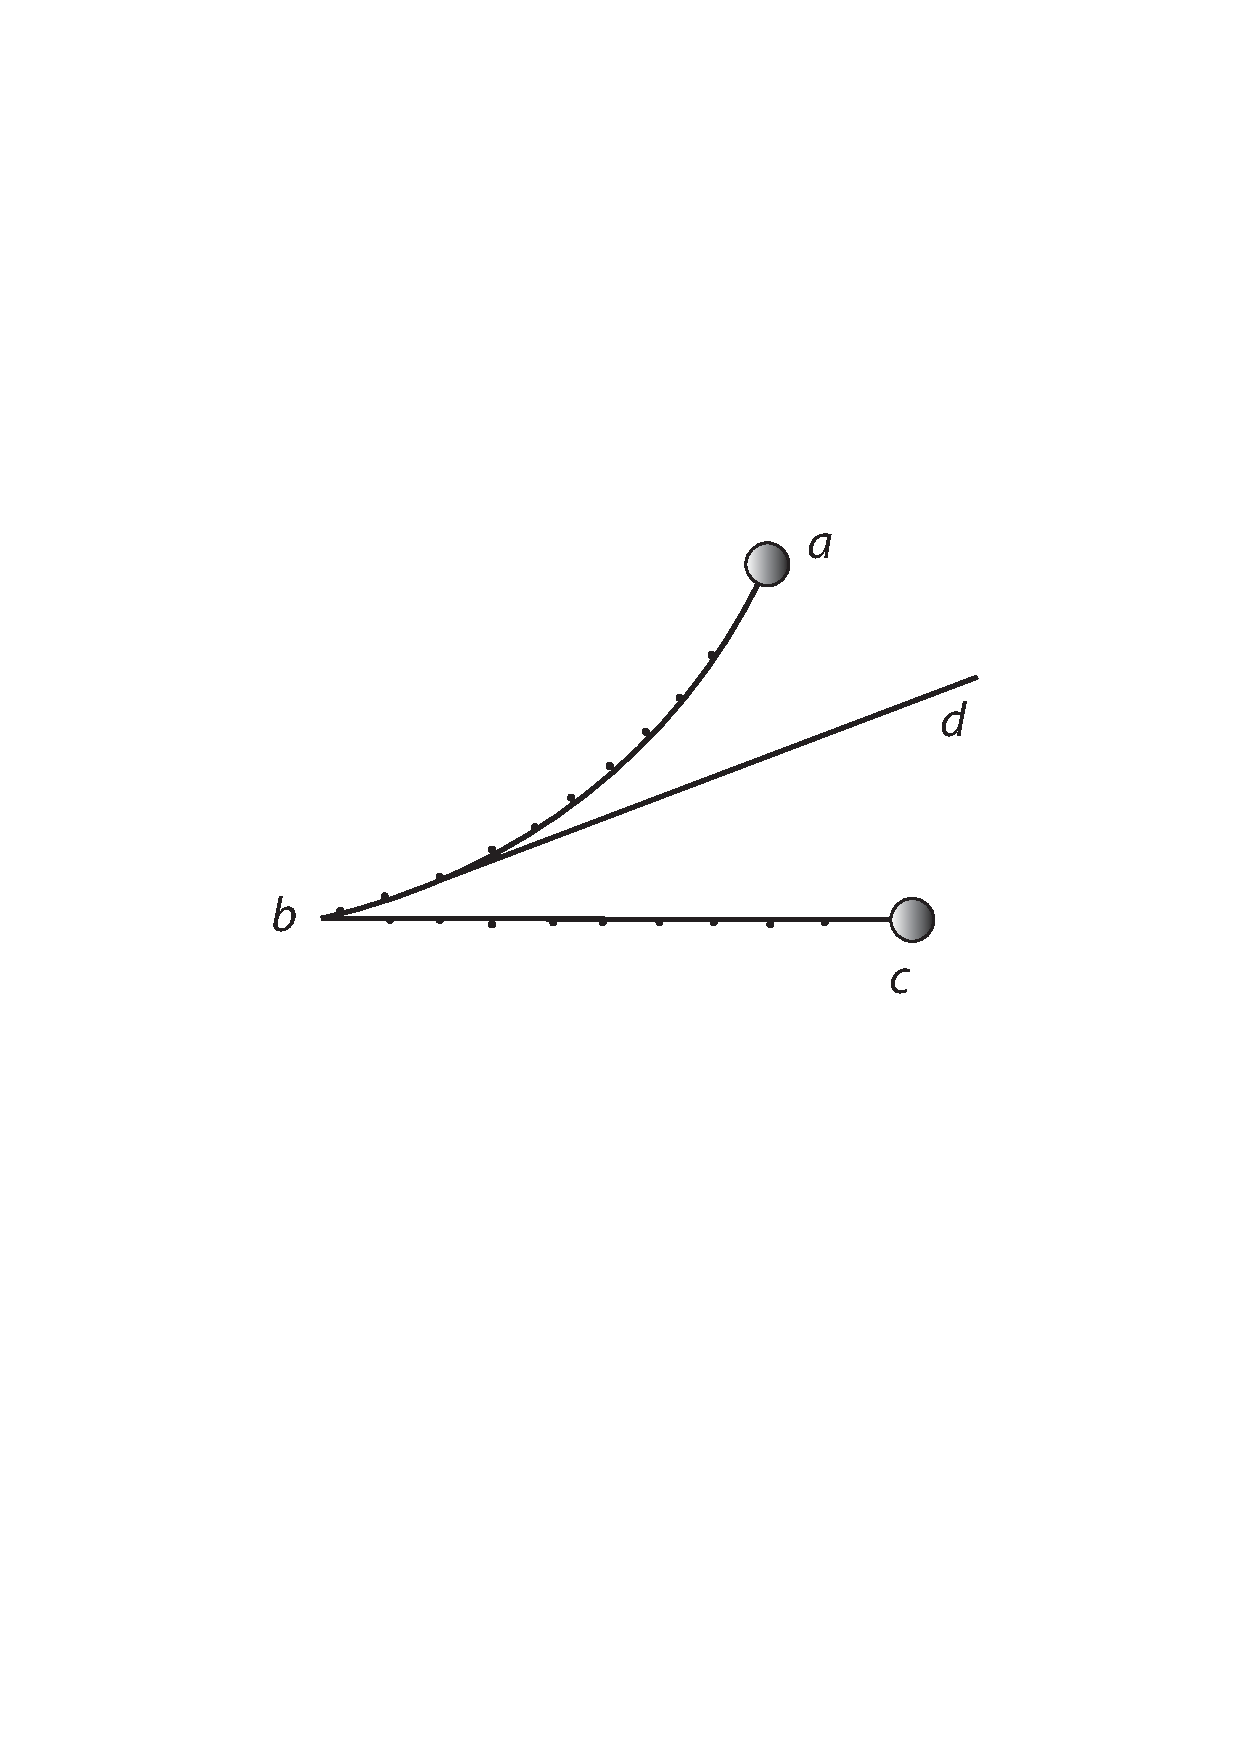
\includegraphics[trim = 0mm 0mm 0mm 0mm, clip, width=0.36\textwidth]{images/lh374_34rkonvertiert.pdf}\\
 \noindent \centering [\textit{Fig. 1}] 
  \pend
 


%    \input{gesamttex/edit/LH037_04_034v.tex} %in34r




\chapter[\scriptsize\uppercase{Analyse von Wallis' Mechanica}]{\uppercase{Analyse von Wallis' Mechanica}
\newline\lbrack XXX \textendash\ XXX\rbrack}
\addcontentsline{toc}{chapter}{\thechapter\enskip Analyse von Wallis' Mechanica \lbrack XXX \textendash\ XXX\rbrack}
\vspace{8mm}
%    \input{gesamttex/edit/LH035_14_02_117r.tex}
%    \input{gesamttex/edit/LH035_14_02_117v.tex}
%    \input{gesamttex/edit/LH035_14_02_118r.tex}
%    \input{gesamttex/edit/LH035_14_02_118v.tex}
%    \input{gesamttex/edit/LH035_14_02_119r.tex}
%    \input{gesamttex/edit/LH035_14_02_119v.tex}
%    \input{gesamttex/edit/LH035_14_02_120r.tex}
%    \input{gesamttex/edit/LH035_14_02_120v.tex}
%    \input{gesamttex/edit/LH035_14_02_121r.tex}
%    \input{gesamttex/edit/LH035_14_02_121v.tex}
%    \input{gesamttex/edit/LH035_14_02_122r.tex}
%    \input{gesamttex/edit/LH035_14_02_122v.tex}
%    \input{gesamttex/edit/LH035_14_02_123r.tex}
%    \input{gesamttex/edit/LH035_14_02_123v.tex}
%    \input{gesamttex/edit/LH035_14_02_124r.tex}
%    \input{gesamttex/edit/LH035_14_02_124v.tex}


%\renewcommand{\chapterpagestyle}{firstchapter} %HSieb
%\renewcommand*{\chapterheadstartvskip}{\vspace*{15.5ex}} %HSieb





% Mechanica - U H R E N  UND  P E N D E L

\clearpage{\pagestyle{empty}\cleardoublepage}
\addtocontents{toc}{\vspace{5mm}}
\addpart[\large\uppercase{II.B. Mechanica \textendash\  Uhren und Pendel}]{\large\protect\textso{II.B. Mechanica \textendash  Uhren und Pendel}}
\clearpage{\pagestyle{empty}\cleardoublepage}

\renewcommand{\chapterpagestyle}{firstchapter}
\renewcommand*{\chapterheadstartvskip}{\vspace*{15.5ex}}

\markleft{\scriptsize\uppercase{II.B. Mechanica \textendash\  Uhren und Pendel}}


\chapter[\scriptsize\uppercase{De variis rationibus procurandi motus uniformis}]{\uppercase{De variis rationibus procurandi motus uniformis}
\newline\lbrack Fr\"{u}hjahr \textendash\ Sommer 1671\rbrack}
\addcontentsline{toc}{chapter}{\thechapter\enskip De variis rationibus procurandi motus uniformis \lbrack Fr\"{u}hjahr \textendash\ Sommer 1671\rbrack 
%\newline \href{http://leibnizviii.bbaw.de/Leibniz_Reihe_8/De\%2Bpraestando\%2Bmotu\%2Buniformi\%2Bpendulo/LH035\%252C15\%252C06_059r/index.html}{059r}
%\href{http://leibnizviii.bbaw.de/pdf/De\%2Bpraestando\%2Bmotu\%2Buniformi\%2Bpendulo/LH035\%252C15\%252C06_059r/LH035,15!06_059+ra-11068.jpg}{Folio}
}
\markleft{\scriptsize\uppercase{II.B Mechanica. Uhren und Pendel}}
\vspace{8mm}
             
               
                \begin{ledgroupsized}[r]{120mm}
                \footnotesize 
                \pstart                
                \noindent\textbf{\"{U}berlieferung:}   
                \pend
                \end{ledgroupsized}
            
              
                            \begin{ledgroupsized}[r]{114mm}
                            \footnotesize 
                            \pstart \parindent -6mm
                             \makebox[6mm][l]{\textit{L}}Aufzeichnung: LH XXXV 15, 6 Bl. 59. 1 Bl. 8\textsuperscript{o} ungleichm\"{a}{\ss}ig beschnitten. 2 S.\\KK 1, Nr. 194 C \pend
                            \end{ledgroupsized}
                %\normalsize
                \vspace*{5mm}
                \begin{ledgroup}
                \footnotesize 
                \pstart
            \noindent\footnotesize{\textbf{Datierungsgr\"{u}nde}: Leibniz beschreibt verschiedene Mechanismen zur Erzeugung einer gleichf\"{o}rmigen Bewegung und beruft sich hierbei vor allem auf Francesco Lana,
dessen \cite{00069}\textit{Prodromo} (1670) er vermutlich in der zweiten H\"{a}lfte 1671 zur Optik exzerpiert hat (\cite{01103}\textit{LSB} VIII,~1 N. 16).
Im vorliegenden St\"{u}ck erw\"{a}hnt Leibniz sein \textit{Perpetuum mobile},
dessen Konstruktion er im Juni 1671 beschreibt (\cite{01187}\textit{LSB} VIII,~1 N. 59).
Auf dasselbe Jahr geht die Arbeit an seiner hier ebenfalls erw\"{a}hnten Rechenmaschine für die vier Grundrechenarten (\textit{Panarithmicum}) zurück.
Über Kirchers \textit{Heliotropium} hat sich Leibniz beim Jesuiten selbst im Mai und Juni 1670 informiert (\cite{01188}\textit{LSB} II,~1, 2. Aufl., N. 20a und N. 23).
Das vorliegende Stück mag daher zeitnah zu den Lana-Exzerpten entstanden sein.}
                \pend
                \end{ledgroup}
            
                \vspace*{8mm}
                \pstart
                \noindent
                 [59 r\textsuperscript{o}] 
                \pend
                \pstart 
                \normalsize
           \begin{center}\edtext{Motum uniformem praestitit Galil.\protect\index{Namensregister}{\textso{Galilei}, Galileo (1564-1642)}\edtext{}{\lemma{Galil.}\Cfootnote{\textsc{G. Galilei, }\cite{00050}\textit{Discorsi}, Leiden 1638, S. 97f. (\textit{GO} VIII, S. 140f.).}}, perp. L.\edtext{}{\lemma{L.}\Cfootnote{\textsc{F. Lana, }\cite{00069}\textit{Prodromo}, Brescia 1670, S. 80-85.}}}{\lemma{}\Bfootnote{Motum [...] perp. L. \textit{erg.} \textit{L}\ }} 
           \end{center}  
           \pend 
           \pstart \vspace{0,5em} \noindent \textso{Motum uniformem }\protect\index{Sachverzeichnis}{motus uniformis}pendulo\protect\index{Sachverzeichnis}{pendulum} praestari primus orbi aperuit Galilaeus\protect\index{Namensregister}{\textso  {Galilei}, Galileo (1564-1642)}, eundem praestari restitutione elateris\protect\index{Sachverzeichnis}{elater} alii addidere, et huic principio innititur Horologiorum\protect\index{Sachverzeichnis}{horologium} portatilium Elasticorum constructio, quae non valde antiqua sunt.  Posset ergo vibratione chordarum, restitutione arcuum\protect\index{Sachverzeichnis}{arcus}, pulsatione campanarum\protect\index{Sachverzeichnis}{campana} vel tympanorum\protect\index{Sachverzeichnis}{tympanum} haberi motus uniformis\protect\index{Sachverzeichnis}{motus uniformis}. Sed chordarum tympanorumque\protect\index{Sachverzeichnis}{tympanum} vibratio invisibilis in parvo visibilis futura si quid iis longi radii applicetur. Sed cum constet chordas in tensione sua mirifice variare (quanquam appenso pondere mederi liceat, quod remittentem attrahat magis) sit vero etiam applicatio futura difficillima, nunc quidem de hac re non dicemus. Etsi applicatione
           \pend
           \newpage
           \pstart\noindent commoda reperta[,] res mirae perfectionis, futura sit machinula, cum non dubitem unam chordae vibrationem centesima millesima horae parte  et fortasse minore absolvi. Ergo si vibratio quaelibet moveret rotam subtilissimam, ita constructam ut reciprocatione tamen eodem  semper iret, et redeundo etiam prorsum ageret, \edtext{uti Lana\protect\index{Namensregister}{\textso{Lana de Terzi}, Francesco 1631-1687} habet.}%
{\lemma{uti Lana habet}\Cfootnote{\cite{00069}a.a.O., S.~80-85.}} Mirabilis subtilitatis esset haec temporis divisio, pone semper finem vibrantis unius \edtext{facere pulsationem alterius,}%
{\lemma{facere}\Bfootnote{%
\textit{(1)} vibrationem alterius
\textit{(2)} pulsationem alterius, \textit{L}}} et rem in circulum redire, applicata nostra \edtext{m.~p.}{\lemma{m.~p.}\Cfootnote{motus perpetui.}} machina.  Haberet ea res haec commoda, \edtext{quod chorda valide}{\lemma{quod}\Bfootnote{\textit{(1)} valde \textit{(2)} chorda valide \textit{L}}} an leniter pulsaretur, nihil interesset, ut constat ex sono\protect\index{Sachverzeichnis}{sonus} chordarum  in musicis. Nam etsi vehementia mutetur, sonus\protect\index{Sachverzeichnis}{sonus} tamen id est vibrationum isochronismus idem est. Applicatione tantum vel ponderis vel \edtext{alterius moventis ita  facta, daß die Seite sich selbst stimme.}%
{\lemma{alterius}\Bfootnote{%
\textit{(1)} rei ita fac
\textit{(2)} moventis ita  facta,
\textit{(a)}\ ut chorda
\textit{(b)}\ daß [...] stimme.
\textit{L}}} Ita  tamen ut a pulsante non possit retrahi illud, quia scil.  in alterum forte latus aliqua cum applicatione trahit,  aut lente per circumvolutiones trochleares\protect\index{Sachverzeichnis}{trochlea}. Ut autem \edtext{[commodissime]}{\lemma{commodisse}\Bfootnote{\textit{L \"{a}ndert Hrsg.}}} numerari possint minuta, adhibenda Logistica decimalis,  atque ea applicatio \edtext{quam meo}{\lemma{quam}\Bfootnote{\textit{(1)} ad \textit{(2)} meo \textit{L}}}\textso{ Panarithmico }destinavi, rotarum ita sibi applicatarum, ut una semel circumacta alterius  decimam tantum partem circumagat, \edtext{adde Lanam.\protect\index{Namensregister}{\textso{Lana de Terzi}, Francesco 1631-1687}}%
{\lemma{adde Lanam}\Cfootnote{\cite{00069}a.a.O., Tafel XVI.}} Haec  de chordis, solida: campanae\protect\index{Sachverzeichnis}{campana}, tympana\protect\index{Sachverzeichnis}{tympanum} non sunt commodi usus,  nisi construatur machina tantae subtilitatis, ut solo sono\protect\index{Sachverzeichnis}{sonus} moveatur  uti chorda tensa \edtext{[altera]}{\lemma{aliter}\Bfootnote{\textit{L ändert Hrsg.}}} similiter tensa sonante resonat. Ergo  si campana\protect\index{Sachverzeichnis}{campana} sonans moveat chordam solo sono\protect\index{Sachverzeichnis}{sonus}, chorda mota circumagat aliquid quod vicissim eundem sonum\protect\index{Sachverzeichnis}{sonus} rursus imprimat[,]
campanae\protect\index{Sachverzeichnis}{campana} habebitur circulatio et uniformitas
\edtext{summa.
[59~v\textsuperscript{o}]
Arcuum [restitutione]}%
{\lemma{summa. [59~v\textsuperscript{o}]}\Bfootnote{%
\textit{(1)} Arcubus ita forsan uti licebit, atque his
\textit{(2)} Arcuum restitutio
\textit{L \"{a}ndert Hrsg.}}} quia sensibilissima, celerrima tamen facilius nos uti posse censeo. Sit circulus aliquis vel annulus  meris arcubus circumdatus qui contrahente se seu minuente  circulo tendantur[,] red-aperiente
\edtext{restituantur. Possint}{\lemma{restituantur.}\Bfootnote{\textit{(1)} Applicat \textit{(2)} Possint \textit{L}}} tamen et sine circuli dilatatione aperiri a motis  tantum quibusdam impedimentulis, ita ut arcus unus restitutus, ubi primum ad statum naturalem\protect\index{Sachverzeichnis}{status naturalis} rediit tangat  alium eumque similiter liberet. Ita in toto dato spatio  liberabuntur: et quidem uniformiter, quia restitutiones ejusdem arcus, etiam inaequaliter tensi, sunt Isochronae. Nec erit hic quae in Elatere\protect\index{Sachverzeichnis}{elater} communi se restituente irregularitas, quia eum multa morantur, hic  cum restitutio sit pene momentanea, non potest esse  sensibilis irregularitas: restitutione chordae ultimae aperiatur circulus. Interea apertura sua chordae istae contraxere seu retendere circulum alium vicinum vel si  lubet ejusdem partem oppositam. Atque ita motus continuabitur uniformiter. Non dubito decem millia  restitutionum ejus\-modi una hora fieri posse. Habebitur  ergo horae \edtext{pars decies}{\lemma{pars}\Bfootnote{\textit{(1)} 10 \textit{(2)} decies \textit{L}}} millesima, forte non minore  quam in pendulis\protect\index{Sachverzeichnis}{pendulum} regularitate, nullo autem jactationis maritimae metu. Ita ut applicari quoque horologiis portatilibus\protect\index{Sachverzeichnis}{horologium portabilium} possit. Porro ope Logisticae decimalis rotis pluribus applicatae, facile poterit etiam millesies millesima pars anni, si scil. ponamus integro anno currere posse horologium\protect\index{Sachverzeichnis}{horologium}, vel septimanae  saltem (quanquam applicatione possit esse perpetuum)  nullo negotio exhiberi. Una superest ratio procurandi motus uniformis\protect\index{Sachverzeichnis}{motus uniformis}. Nimirum per magnetem\protect\index{Sachverzeichnis}{magnes}, constat acum  libratam diu vacillare antequam requiescat. Quaeritur ergo an vacillationes esse possint isochronae. Item an ipse motus tendendi ad polum isochronus quacunque posita distantia, ita scil.  ut si remota sit longius, moveatur celerius. Sed hic subest  ea difficultas, quod perpendicularis situs requiritur. Ergo  videndum an attractione magnetica\protect\index{Sachverzeichnis}{attractio magnetica} quicquam agi possit, ita  scil. ut acus attracta accessu aperiat aliquid quo repercutiatur, idque nova attractione\protect\index{Sachverzeichnis}{attractio} rursus claudat, novo tactu rursus \edtext{aperiat. Rursus claudet, si in attrahendo}{\lemma{aperiat}\Bfootnote{\textit{(1)} , attrahet \textit{(2)} . Rursus claudet, si in attrahendo \textit{L}}} applicetur spirae\protect\index{Sachverzeichnis}{spira} alicui vel vecti, sed non erit celeritas\protect\index{Sachverzeichnis}{celeritas} tanta[,]  puto tamen absolvi posse intra minutum secundum. Machina pure magnetica sine omni elatere. A pondere si ab amico attrahatur, semel allapsa inimicum inveniat, et  ab eo repellatur. \edtext{Heliotropium Kircheri\protect\index{Namensregister}{\textso{Kircher}, Athanasius 1602-1680}}%
{\lemma{Heliotropium Kircheri}\Cfootnote{\textsc{A. Kircher, }\cite{00067}\textit{Magnes}, Rom 1654, S. 508.}} habet etiam motum uniformem\protect\index{Sachverzeichnis}{motus uniformis}.\pend
 


 


 

 

 


 


 


 


 


%      \input{gesamttex/edit/LH035_15_06_059v.tex} %v-text in r


\renewcommand*{\chapterpagestyle}{scrheadings}
\renewcommand*{\chapterheadstartvskip}{\vspace*{-5mm}}

\chapter[\scriptsize\uppercase{Chronologia. Efficere horologia accurata}]{\uppercase{Chronologia. Efficere horologia accurata}
\newline\lbrack 2. H\"{a}lfte 1672\rbrack}
\addcontentsline{toc}{chapter}{\thechapter\enskip Chronologia. Efficere horologia accurata \lbrack 2. H\"{a}lfte 1672\rbrack 
%\newline \href{http://leibnizviii.bbaw.de/Leibniz_Reihe_8/Chronologia.\%2BEfficere\%2Bhorologia\%2Baccurata/LH035\%252C15\%252C06_058r/index.html}{058r}
%\href{http://leibnizviii.bbaw.de/pdf/Chronologia.\%2BEfficere\%2Bhorologia\%2Baccurata/LH035\%252C15\%252C06_058r/LH035,15!06_058+ra-11065.jpg}{Folio}
}
\vspace{8mm}
          
               
                \begin{ledgroupsized}[r]{120mm}
                \footnotesize 
                \pstart                
                \noindent\textbf{\"{U}berlieferung:}   
                \pend
                \end{ledgroupsized}
            
              
                            \begin{ledgroupsized}[r]{114mm}
                            \footnotesize 
                            \pstart \parindent -6mm
                             \makebox[6mm][l]{\textit{L}}Aufzeichnung: LH XXXV 15,  6 Bl. 58. 1 Bl. 4\textsuperscript{o}. 1 S. auf Bl.~58~r\textsuperscript{o}.
Bl.~58~v\textsuperscript{o} leer.  \\KK 1, Nr. 194 B \pend
                            \end{ledgroupsized}
                %\normalsize
                \vspace*{5mm}
                \begin{ledgroup}
                \footnotesize 
                \pstart
            \noindent\footnotesize{\textbf{Datierungsgr\"{u}nde}: In der von Leibniz erw\"{a}hnten Stelle aus Monconys' \textit{Journal des voyages}\cite{00118}
wird \"{u}ber eine Methode zur Regulierung der Pendelbewegung berichtet, die auf Isaac Vossius zur\"{u}ckgeht.
Zentrales Element dieser Methode ist ein Siphon, dessen Konstruktion einen stetigen Ausfluss erm\"{o}glicht.
Leibniz hat diese Idee im Stück \cite{00269}\textit{LSB} VIII,~1 N.~63 aufgegriffen und zu einer Wasseruhr fortentwickelt.
Das daf\"{u}r entworfene Z\"{a}hlwerk entspricht in seiner Grundkonstruktion dem im vorliegenden Text beschriebenen.
Aufgrund dieser inhaltlichen \"{U}bereinstimmung kann eine zeitnahe Entstehung beider Texte angenommen werden.
Die hieraus resultierende Datierung lässt sich ferner dadurch st\"{u}tzen,
dass Leibniz im vorliegenden Text einen Vergleich mit Vakuumph\"{a}nomenen liefert,
mit denen er sich gleichfalls in der zweiten Jahresh\"{a}lfte 1672 beschäftigte (siehe etwa \cite{01190}\textit{LSB} VIII,~1 N.~41).}
                \pend
                \end{ledgroup}
            
                \vspace*{8mm}
               \pstart%
\noindent%
\normalsize%
[58~r\textsuperscript{o}]
\pend%
\pstart%
\noindent%
\centering%
\edtext{Chronologia}{\lemma{Chronologia}\Bfootnote{\textit{erg. L}}}
\pend%
\vspace{0,5em}%
\pstart%
\noindent%
\textso{Efficere Horologia accurata.}
Vid. Isaaci Vossii\protect\index{Namensregister}{\textso{Vossius}, Isaac 1618-1689} consilium
\edtext{apud Monconisium.\protect\index{Namensregister}{\textso{Monconys} (Monconisius), Balthasar de 1611-1665}}%
{\lemma{apud Monconisium}\Cfootnote{\textsc{B. de Monconys,}\cite{00118} \textit{Journal des voyages}, Teil II, Paris 1666, S.~154.}} Iniri possunt rationes variae, si quolibet ictu  penduli aperiretur superius foramen, unde excideret  sive liquor sive granum aliquod granum grano aequale, aut gutta\edtext{ guttae, quae lapsu suo priorem semper impetum de novo  imprimerent pendulo et praeterea laberentur in vas quod implendo signarent numerum in eo notatum}{\lemma{guttae,}\Bfootnote{\textit{(1)}\ quibus notarentur \textit{(2)}\ quae [...] notatum \textit{L}}} vibrationum. Deberet vitreum seu perspicuum esse.  Posset esse in cochleam\protect\index{Sachverzeichnis}{cochlea} contortum, notandis exactius  gradibus. Aut si rectilineum esset, gradus designati  paralleliter deberent transversis subdividi  si cochleare, eousque contortura opus esset, quousque  adhuc sive gutta, sive granum per obliquitatem  descendere possent; nam in cochlea\protect\index{Sachverzeichnis}{cochlea} nimis obliqui  siccum non descenderet, liquidum descenderet sed  tarde. Quid si ut in experientia vacui\protect\index{Sachverzeichnis}{experientia vacui} qualibet  apertura immitteretur aer, qui sive hydrargyrum\protect\index{Sachverzeichnis}{hydrargyrus}  sive aquam pendentem magis descendere faceret  sed tunc deesset causa perpetuo percutiens pendulum\protect\index{Sachverzeichnis}{pendulum}. Liquidis non facile designari potest  numerus vibrationum, etsi alia divisio in minuta  forte tertia signari possit. Siccis potest. Caeterum  ita instituto instrumento nescio an obesse possit  situs \edtext{non perpendicularis}{\lemma{situs}\Bfootnote{\textit{(1)}\ perpendicularis \textit{(2)}\ non perpendicularis. \textit{L}}}. Forte  rectius res geretur, si qualibet vibratione rotulae  alicujus aculeus novus descendat descensuque pendulum\protect\index{Sachverzeichnis}{pendulum}  rursus, aequaliter semper, impellat. In rotae aculeis  designari numerus potest, sit \edtext{v.g.}{\lemma{sit}\Bfootnote{\textit{(1)} alia rota major p \textit{(2)} v.g. \textit{L}}}  quaelibet vibratio unius minuti \edtext{secundi}{\lemma{minuti}\Bfootnote{\textit{(1)}\ tertii \textit{(2)}\ secundi. \textit{L}}}. 
            Erunt  in rota aculei $60 \smallfrown 60$ seu 3600.  
            Sit alia rota major quae una gyratione minoris \edtext{unum sui gradum absolvat}{\lemma{minoris}\Bfootnote{\textit{(1)}\ absolvatur \textit{(2)}\ unum sui gradum absolvat, \textit{L}}}, divisa in gradus 60, notandis minutis primis, denique  sit rota pro horis, cujus unus gradus qualibet  secundae rotae gyratione absolvatur, tot quot  sunt horae.\pend 
            \pstart  Damit dem pendulo\protect\index{Sachverzeichnis}{pendulum} keine jactation  schade, auch da \edtext{es}{\lemma{da}\Bfootnote{\textit{(1)}\ $\langle$man$\rangle$ \textit{(2)}\ es \textit{L}}} par un ressort  ge\-macht werden solte, dessen unvermeidliche irregularitaten durch luftspannung\protect\index{Sachverzeichnis}{Elastizit\"{a}t der Luft}  und sonsten, nicht in das pendulum\protect\index{Sachverzeichnis}{pendulum} transferirt, konte also geschehen, wenn \edtext{ein rad}{\lemma{wenn}\Bfootnote{\textit{(1)}\ durch \textit{(2)}\  ein  \textit{(a)}\ rath \textit{(b)}\ rad \textit{L}}} so soviel zacken oder abtheilung  hatte, als das pendulum in einer stunde vibrationes thut  pone 3600. Wenn alle minuta 2\textsuperscript{da} eine vibration  geschehe, herunter iedes mahl mit einem zacken stiege so oft das pendulum\protect\index{Sachverzeichnis}{pendulum} mit einer vibration ihm den  weg offnet, aber nicht mehr als ein zacken dieweil  mit dem anderen das pendulum\protect\index{Sachverzeichnis}{pendulum} wieder her\"{u}bergestossen, und von neuen vibrirt w\"{u}rde. Damit aber  die vibration allezeit egal bleiben soll der  ictus alle mahl fortior seyn, als pro vibratione  n\"{o}thig, und doch die vibratio wegen des anstosses  auf beyden seiten allezeit klein \edtext{bleiben. Es}{\lemma{bleiben.}\Bfootnote{\textit{(1)}\ Der \textit{(2)}\  Es \textit{L}}} werde also der ictus bald st\"{a}rcker bald  schw\"{a}cher, dennoch solange er nicht gar  zu sehr heruntersteiget, so doch per constructionem nicht geschehen kan wird die vibration, auch ungeachtet der obliquit\"{a}t gleich bleiben.  \pend 
 


 


 


 


 


 


 


 


 


 




\chapter[\scriptsize\uppercase{Quomodo motus penduli magnete effici possit}]{\uppercase{Quomodo motus penduli magnete effici possit}
\newline\lbrack 2. H\"{a}lfte 1672\rbrack}
\addcontentsline{toc}{chapter}{\thechapter\enskip Quomodo motus penduli magnete effici possit \lbrack 2. H\"{a}lfte 1672\rbrack 
%\newline \href{http://leibnizviii.bbaw.de/Leibniz_Reihe_8/Quomodo\%2Bmotus\%2Bpenduli\%2Bmagnete\%2Beffici\%2Bpossit/LH035\%252C15\%252C06_060r/index.html}{060r} 
%\href{http://leibnizviii.bbaw.de/pdf/Quomodo\%2Bmotus\%2Bpenduli\%2Bmagnete\%2Beffici\%2Bpossit/LH035\%252C15\%252C06_060r/LH035,15!06_060+ra-11071.jpg}{Folio}
%\href{http://leibnizviii.bbaw.de/Leibniz_Reihe_8/Quomodo\%2Bmotus\%2Bpenduli\%2Bmagnete\%2Beffici\%2Bpossit/LH035\%252C15\%252C06_060v/index.html}{060v}
%\href{http://leibnizviii.bbaw.de/pdf/Quomodo\%2Bmotus\%2Bpenduli\%2Bmagnete\%2Beffici\%2Bpossit/LH035\%252C15\%252C06_060v/LH035,15!06_060+va-11073.jpg}{Folio}
}
\vspace{8mm}
                      
                \begin{ledgroupsized}[r]{120mm}
                \footnotesize 
                \pstart                
                \noindent\textbf{\"{U}berlieferung:}   
                \pend
                \end{ledgroupsized}
            
              
                            
                            \begin{ledgroupsized}[r]{114mm}
                            \footnotesize 
                            \pstart \parindent -6mm
                            \makebox[6mm][l]{\textit{L}}Aufzeichnung: LH XXXV 15, 6 Bl. 60. 1 Bl. 8\textsuperscript{o}, ungleichm\"{a}{\ss}ig beschnitten. 2 S. \\KK 1, Nr. 194 D \pend
                            \end{ledgroupsized}
                %\normalsize
                \vspace*{5mm}
                \begin{ledgroup}
                \footnotesize 
                \pstart
            \noindent\footnotesize{\textbf{Datierungsgr\"{u}nde}: Im vorliegenden Stück N.~87 %?? = LH035,15,06_060 = Quomodo penduli motus magnete effici possit
sucht Leibniz nach einer L\"{o}sung f\"{u}r die Stabilisierung des Gangs von Pendeluhren,
indem er die Anwendung von Magneten in Erwägung zieht.
Mit der eingangs angedeuteten Methode Isaac Vossius' setzt er sich auch in der Aufzeichnung N.~84 %?? = LH035,15,06_058 = Chronologia. Efficere horologia accurata
auseinander.
Der Hinweis auf die L\"{a}ngengradbestimmung im zweiten Teil von N.~87 %?? = LH035,15,06_060 = Quomodo penduli motus magnete effici possit
dürfte sich auf das St\"{u}ck \cite{01072}\textit{LSB} VIII,~1 N.~6\textsubscript{2} beziehen, 
welches editorisch auf die zweite H\"{a}lfte 1672 datiert wurde.
N.~87 %?? = LH035,15,06_060 = Quomodo penduli motus magnete effici possit
könnte somit zeitnah entstanden sein.}
                \pend
                \end{ledgroup}
            
                \vspace*{8mm}
                \pstart 
                \normalsize \noindent
            [60~r\textsuperscript{o}] \selectlanguage{ngerman}Den Motum penduli zu continuiren siehe was Vossius\protect\index{Namensregister}{\textso  {Vossius}, Isaac (1618-1689)} vorschl\"{a}gt\selectlanguage{latin} apud\edtext{ Monconys}{\lemma{Monconys}\Cfootnote{\textsc{B. de Monconys, }\cite{00134}\textit{Journal des voyages}, Teil II, Paris 1666, S. 154.}} pag. 154. \textit{Voyage des pays bas}.\protect\index{Namensregister}{\textso {Monconys}, Balthasar de (1611-1665)} Hugenius\protect\index{Namensregister}{\textso  {Huygens}, Christiaan (1629-1695)} mus eine andre  manier haben, so mir noch nicht bewust. Fortasse optime per magnetem\protect\index{Sachverzeichnis}{magnes}, si nimirum penduli\protect\index{Sachverzeichnis}{pendulum} inferior  pars esset acus magneti\protect\index{Sachverzeichnis}{acus magnetica} affricta, sed contrario quam qui suppositus est polo. Haec a polo repulsa redelaberetur gravitate\protect\index{Sachverzeichnis}{gravitas naturalis} naturali, et praeterveheret impetu in alteram partem, redux  rursus impelleretur, et ita porro. Modo scilicet proportio ea sit, ut impetu labentem non possit, quiescentem aut progredientem possit vincere \edtext{magnes\protect\index{Sachverzeichnis}{magnes}.
An fortasse aptius ita magnes}{\lemma{magnes.}\Bfootnote{\textit{(1)}\ Sed idem \textit{(a)}\ si ta \textit{(b)}\ aptius si tam fortis \textit{(2)}\ An [...] magnes \textit{L}}} sine ullo pendulo\protect\index{Sachverzeichnis}{pendulum} et perpetuum simul et uniformem efficere motum\protect\index{Sachverzeichnis}{motus perpetuus}\protect\index{Sachverzeichnis}{motus uniformis } potest. \edtext{Finge}{\lemma{potest.}\Bfootnote{\textit{(1)}\ Esto \textit{(2)}\ Finge \textit{L}}} magnetem\protect\index{Sachverzeichnis}{magnes} ita fortiter repellere  acum, ut totam circumagat, atque ita denuo repellere \edtext{possit. Si unus magnes}{\lemma{possit.}\Bfootnote{\textit{(1)}\ Si hoc procederet \textit{(2)}\ Si unus magnes \textit{L}}} non satis fortis  esset applicandus esset alter similiter, traderentur sibi  plures per manus. Quilibet admitteret, quia \edtext{ab}{\lemma{quia}\Bfootnote{\textit{(1)}\ ob \textit{(2)}\ ab \textit{L}}}  obliquo et a tergo, et ab alio magnete\protect\index{Sachverzeichnis}{magnes} impulsam\protect\index{Sachverzeichnis}{impulsus}  repelleret ubi sibi e directo venit. Erunt ergo  omnes periodi uniformes. Etsi non forte partes periodorum  finge quolibet minuto secundo periodum absolvi,  applicetur logistica decimalis, ut dixi. Sed  hoc artificio, ut non sit opus magnetibus\protect\index{Sachverzeichnis}{magnes} aliquando movere  omnes omnino \edtext{gyros;}{\lemma{gyros;}\Bfootnote{\textit{(1)}\ sed ta \textit{(2)}\ quod \textit{L}}} quod alioquin fieret nonnunquam concurrentibus aliquando \edtext{revolutionibus. Verum}{\lemma{revolutionibus.}\Bfootnote{\textit{(1)}\ Sed \textit{(2)}\ Verum \textit{L}}} ut gyrus propior aperiat tantum aliquid quo alter  se sponte moveat. Haec machinula\protect\index{Sachverzeichnis}{machinula} esset pure magnetica independens a gravitate\protect\index{Sachverzeichnis}{gravitas} et Elatere\protect\index{Sachverzeichnis}{elater}, atque  ita fortasse omnium quae cogitari possunt ad horologia\protect\index{Sachverzeichnis}{horologium}  aptissima, aeri excludendo includendus magnes\protect\index{Sachverzeichnis}{magnes} vitro  sigillato, cujus fortasse lateribus includatur aqua, aut spiritu vini\protect\index{Sachverzeichnis}{spiritus vini} excludendae tanto rectius aeri. Et conservandis  viribus magnetum\protect\index{Sachverzeichnis}{magnes}. Possunt et plures acus esse in  eodem circulo, eadem quae magnetum\protect\index{Sachverzeichnis}{magnes} est distania. Res  certa est: modo hoc unum obtineatur magnetes\protect\index{Sachverzeichnis}{magnes} fortius repellere [60~v\textsuperscript{o}] et attrahere in axe continuato, quam in linea  aliqua obliqua. Quod mihi rationi consentaneum videtur, si quod maxime. 
Quaerenda:%
\newline\indent%
1) motus perp.\protect\index{Sachverzeichnis}{motus perpetuus}%
\newline\indent%
2) motus uniformis,\protect\index{Sachverzeichnis}{motus uniformis}
ope penduli,\protect\index{Sachverzeichnis}{pendulum}
Elateris,\protect\index{Sachverzeichnis}{elaterium}
magnetis;\protect\index{Sachverzeichnis}{magnes}
omnium si possibile praestare ea de quibus alibi,
ut nimis celeriter motum aut nimis tarde tanto magis excitetur aut retardetur ab applicato.%
\newline\indent%
3) motus
perpetuo respiciens datam plagam, seu quiddam absolute immobile ex dato centro,
hoc fiet meridiano\protect\index{Sachverzeichnis}{meridianus} universali
\edtext{Grandamici\protect\index{Namensregister}{\textso{Grandami}(Grandamicus), Jacques 1588-1672}%
\edtext{.}{\lemma{Grandamici}\Cfootnote{\textsc{J. Grandami}, \cite{00292}\textit{Nova demonstratio immobilitatis terrae}, La Fl\`{e}che 1645, S. 66.}}
\newline\indent%
\textso{Primi}}{\lemma{Grandamici.}\Bfootnote{\textit{(1)}\ Dum posteri \textit{(2)}\ \textso{Primi} \textit{L}}}\textso{ }%
maximus usus ad levandos hominum
\edtext{labores in terra.\protect\index{Sachverzeichnis}{terra}}{\lemma{in terra}\Bfootnote{\textit{erg. L}}}%
\newline\indent%
\textso{Postremi }ad perfecte inveniendas longitudines sine ope coeli, et dirigendos hominum
\edtext{labores in mari.}{\lemma{labores}\Bfootnote{\textit{(1)}\ in terra \textit{(2)}\ in mari. \textit{L}}}
\newline\indent%
Medius ad dirigenda hominum judicia ubique. Primum  dat modum: secundum dat tempus; tertium  dat locum. Quibus tribus omnis mechanica continetur. In machinamento postremo magnetico  potest polus amicus relinqui illaboratus, ne  quid hic agat retinendo. Si circulus  magnetum cum circulo acuum sit in eodem  plano, seu concentricus firmatus: nulla mutatio  machinae sequetur quaecunque sit navis jactatio,  quia gravitatis\protect\index{Sachverzeichnis}{gravitas} tantule variatae per momentaneam rei pendulae jactatae obliquitatem nullam  habet sensibilem proportionem ad vim repulsivam \edtext{magnetis. Sed}{\lemma{magnetis.}\Bfootnote{\textit{(1)}\ Et si \textit{(2)}\ Sed \textit{L}}} observandum tamen an  non tractu temporis fieri possit mutatio sensibilis, et  tunc adhibenda est aequatio. Tum an non crebris  reactionibus desinat inimicitia, aut mutuo destruatur  et quanto tempore possunt et nonnunquam  reparari.  \pend%
\pstart%
\edtext{Cum contactus virtualis sit insensibilis affrictus credibile est acum postremo deventuram unicam.
Quid si ergo talis applicatio ut ab inimico repulsa simul ab amico attrahatur sed qui non satis fortis ad retinendum.
Quia plures repellentes, vel etiam quia interim et alius attrahit aliam.
NB.}{\lemma{Cum [...] NB}\Cfootnote{Auf dem linken Rand von Bl.~60~v\textsuperscript{o}, quer zum übrigen Text.}}
\pend 
 


 


 


 


 


 


 


%    \input{gesamttex/edit/LH035_15_06_060v.tex} %60v in 60r


\chapter[\scriptsize\uppercase{De horologio absoluto}]{\uppercase{De horologio absoluto sive de motu aequabili pure mechanico. Demonstratio geometrica}
\newline\lbrack Ende 1672 \textendash\ Anfang 1673\rbrack}
\addcontentsline{toc}{chapter}{\thechapter\enskip De horologio absoluto sive de motu aequabili pure mechanico. Demonstratio geometrica \lbrack Ende 1672 \textendash\ Anfang 1673\rbrack}
\vspace{8mm}
   %       
               
                \begin{ledgroupsized}[r]{120mm}
                \footnotesize 
                \pstart                
                \noindent\textbf{\"{U}berlieferung:}   
                \pend
                \end{ledgroupsized}
            
              
                            \begin{ledgroupsized}[r]{114mm}
                            \footnotesize 
                            \pstart \parindent -6mm
                           \makebox[6mm][l]{\textit{L}}Konzept:
LH XXXV 11, 13 Bl. 9. 1 Bl. 4\textsuperscript{o}. 1\,\nicefrac{1}{2} S.
\\Cc 2, Nr. 914 \pend
                            \end{ledgroupsized}
                %\normalsize
                \vspace*{5mm}
                \begin{ledgroup}
                \footnotesize 
                \pstart
            \noindent\footnotesize{\textbf{Datierungsgr\"{u}nde}: Die für den Gang von Uhren bereits in N.~85 angeführte Elastizität wird hier in ihrer Wirkungsweise systematisch dargelegt und begrifflich definiert, was sich als fortgesetzte und vertiefende Auseinandersetzung deuten ließe, die im Anschluss an N. 85 etwas später erfolgt sein könnte.}
                \pend
                \end{ledgroup}
            
                \vspace*{8mm}
                \pstart%
\normalsize
\noindent
[9~r\textsuperscript{o}]
\pend%
\pstart%
\centering%
De HOROLOGIO ABSOLUTO\\
sive De Motu aequabili pure mechanico\\
demonstratio Geometrica:
\pend%
            \count\Bfootins=1200 
\pstart 
\vspace*{0.5em} \noindent Axioma:
\edtext{si idem sit agentium\protect\index{Sachverzeichnis}{agens} patientiumque\protect\index{Sachverzeichnis}{patiens} status;
tempora\protect\index{Sachverzeichnis}{tempus} operationum eundem effectum\protect\index{Sachverzeichnis}{effectus} producentium, erunt aequalia.}%
{\lemma{si}\Bfootnote{%
\textit{(1)}\ eaedem sint vires, eademque impedimenta\protect\index{Sachverzeichnis}{impedimentum}
\textit{(2)}\ idem [...] status;
\textit{(a)}\ effectus aequali tempore sequetur 
\textit{(b)}\ tempora [...] aequalia. \textit{L}}}
\pend 
\count\Bfootins=800
\count\Cfootins=1200
\pstart  Corollarium est hoc, axiomatis generalissimi,
quod ejusdem positionis eaedem sunt consequentiae;
unde ejusdem causae, caeteris paribus iidem effectus:
et corpus
\edtext{idem situm eodem modo}{\lemma{idem [...] modo}\Bfootnote{\textit{erg. L}}}
ex eadem altitudine per idem medium eodem tempore sua gravitate\protect\index{Sachverzeichnis}{gravitas}
\edtext{libere}{\lemma{libere}\Bfootnote{\textit{erg. L}}}
descendet; et Elaterium\protect\index{Sachverzeichnis}{elaterium}
\edtext{idem eodem}{\lemma{idem}\Bfootnote{\textit{(1)}\ ad \textit{(2)}\ eodem \textit{L}}}
semper modo
\edtext{tensum, atque mox sibi permissum eodem tempore inde a momento recuperati sui juris ad eundem perveniet statum libertatis.}%
{\lemma{tensum,}\Bfootnote{%
\textit{(1)}\ eodem tempore se liberabit
\textit{(2)}\ atque
\textit{(a)}\ dimissum
\textit{(b)}\ mox libertat
\textit{(c)}\ inde
\textit{(d)}\ mox [...] tempore
\textit{(aa)}\ ad eundem perveniet statum libertatis.
\textit{(bb)}\ inde [...] libertatis. \textit{L}}}
\pend 
%\newpage
\pstart 
\textso{Elaterium }\protect\index{Sachverzeichnis}{elaterium}voco corpus quod figuram vi amissam vi cessante repetit;
quam\textso{ figuram }voco%
\edtext{\textso{ naturalem.}
\newline\indent%
\textso{Tensio }est actio causae figuram corporis Elaterio praediti naturalem mutantis.
\newline\indent%
\textso{Displosio }est actio elaterii figuram naturalem repetentis.
\newline\indent%
\textso{Liberatio }est ablatio impedimenti displosionis.
\newline\indent%
\textso{Detentacula }sunt machinamenta ad elateria detinenda atque detendenda, sive liberanda, apta.\textso{ Detentes }Gallis.
\newline\indent%
Si sint quotcunque Elateria, tensa \textit{A}. \textit{B}. \textit{C}. etc.
ita adhibitis\textso{ detentaculis }disposita,
ut primo \textit{A} liberato et ad certum displosionis statum perveniente, liberetur secundum \textit{B},
et secundo \textit{B} liberato et ad certum displosionis statum perveniente,}%
{\lemma{\textso{naturalem.}}\Bfootnote{%
\textit{(1)}\ Si sint %
\textit{(a)}\ aliquot elateria \textit{A}. \textit{B}. \textit{C}. etc. ita disposita, %
\textit{(aa)}\ ut ipse \textit{A} %
\textit{(bb)}\ atque tensa %
\textit{(b)}\ quotcunque elateria tensa %
\textit{(2)}\ \textso{Tensio} %
\textit{(a)}\ est motus partium corporis Elaterio praediti, quo per vim a figura sua demovetur %
\textit{(b)}\ est motus quo corpus elaterio praeditum mutat %
\textit{(c)}\ est actio [...] displosionis.\,
\textbar\ \textso{Detentacula} [...] Gallis. \textit{erg.} \textbar\
Si sint quotcunque Elateria,
\textbar\ tensa \textit{erg.} \textbar\
\textit{A}. \textit{B}. \textit{C}. etc. ita
\textbar\ adhibitis \textso{detentaculis} \textit{erg.} \textbar\
disposita, ut %
\textit{(aa)}\ sub finem displosionis primi \textit{A}, liberetur secundum \textit{B}, et sub finem displosionis secundi \textit{B} %
\textit{(bb)}\ primo \textit{A} [...] perveniente \textit{L}}}
liberetur tertium \textit{C}, etc.
\edtext{et ita pergatur}{\lemma{et ita pergatur}\Bfootnote{\textit{erg. L}}}
usque dum ultimum
\edtext{quoque faciat}{\lemma{ultimum}\Bfootnote{%
\textit{(1)}\ absolvat %
\textit{(2)}\ quoque faciat \textit{L}}}
displosionem
\edtext{suam; rursusque ultimo ad certum displosionis statum perveniente, liberetur denuo primum \textit{A}, tempus ab}%
{\lemma{suam;}\Bfootnote{%
\textit{(1)}\ tempus a %
\textit{(2)}\ eodemque momento quo ultimum absolvit displosionem suam, %
\textit{(3)}\ rursusque %
\textit{(a)}\ sub finem displosionis ultimi, liberetur iterum primum \textit{A},
(quod interea jam rursus tensum fuisse, et displosionem ultimi in eo statu expectare, supponitur.) %
\textit{(b)}\ ultimo [...] tempus ab \textit{L}}}
uno momento liberationis Elaterii\protect\index{Sachverzeichnis}{elaterium} \textit{A},
\edtext{ad momentum liberationis alterius}%
{\lemma{ad}\Bfootnote{%
\textit{(1)}\ aliud %
\textit{(2)}\ momentum liberationis alterius \textit{L}}} 
proximae sequentis, ejusdem Elaterii\protect\index{Sachverzeichnis}{elaterium} \textit{A},
vocabo\textso{ Periodum }\edtext{\textso{Elateriorum.}
% \newpage%
\newline%
\indent%
Si duae sint Periodi Elateriorum eademque sint Elateria ac detentacula eodem modo sita,
eademque cuilibet Elaterio, quae ante, vis, gradusque tensionis, erunt eae duae periodi inter se aequidiuturnae,}%
{\lemma{\textso{Elateriorum.}}\Bfootnote{%
\textit{(1)}\ Si quodlibet ex Elateriis %
\textit{(a)}\ eodem sem %
\textit{(b)}\ ad eundem semper \textso{tensionis statum} redactum intelligatur, itemque a praecedente ad eundem %
\textit{(aa)}\ tensionis %
\textit{(bb)}\ semper displosionis statum perveniente liberetur;
\textbar\ neque quicquam extrinsecus variationem inducere intelligatur \textit{erg.} \textbar\
Periodi Elateriorum erunt aequidiuturnae. Nam %
\textit{(aaa)}\ ad eu %
\textit{(bbb)}\ eadem sunt %
\textit{(ccc)}\ agentia patientiaque, elateria scilicet numero %
\textit{(aaaa)}\ situque eo %
\textit{(bbbb)}\ magnitudine materia, figura situ; denique ut verbo %
\textbar\ scholarum \textit{erg.}\ \textbar\
dicam, ipso individuo, eadem sunt. %
\textit{(aaaaa)}\ Vi %
\textit{(bbbbb)}\ Status quoque agentium semper idem,
quia eodem semper modo sunt tensa, ad idem scilicet ut ita dicam, punctum, ac tensionis gradum.
Patientium quoque eadem plane dispositio, quoniam ad eundem sem %
\textit{(2)}\ Si duae sint Periodi Elateriorum %
\textit{(a)}\ inter se %
\textit{(b)}\ simillimae, neque quicquam extrinsecus %
\textit{(c)}\ per omnia similes, neque quicquam extrinsecus variationem inducere ponatur, erunt tempora periodorum aequidiuturna %
\textit{(d)}\ eademque sint Elateria
\textbar\ ac detentacula \textit{erg.}\ \textbar\
eodem modo sita, %
\textit{(aa)}\ idemque cujuslibet Elaterii, qui ante, %
\textit{(bb)}\ eademque [...] aequidiuturnae, \textit{L}}}
modo nihil extrinsecus superveniens varietatem inducere ponatur.
\pend 
\count\Bfootins=1000
\count\Cfootins=1200
\pstart  
Hoc enim posito sequetur, duas illas periodos esse per omnia similes,
sive eundem utrobique agentium patientiumque statum esse,
nam per definitionem\textso{ periodi Elateriorum,\protect\index{Sachverzeichnis}{elaterium}}
nulla alia in ipsis agentia atque patientia sunt quam
\edtext{Elateria ac\textso{ detentacula.}}%
{\lemma{Elateria}\Bfootnote{%
\textit{(1)}\ et idem Elaterium quod praecedenti est agens, sequenti est patiens, idem autem qui ante est Elateriorum et instrumenta %
\textit{(2)}\ ac \textso{detentacula.} \textit{L}}}
\edtext{Porro detentacula eadem}%
{\lemma{Porro}\Bfootnote{%
\textit{(1)}\ in Elateriis nihil nisi numerus, et magnitudo, et ma %
\textit{(2)}\ Elateria et %
\textit{(3)}\ detentacula. \textit{(a)}\ et numero {(b)}\ eadem \textit{L}}}
ipsa sunt quae ante, eodemque modo sita:
neque alia in Detentaculis quae rigida intelliguntur,
\edtext{varietas potest concipi.}{\lemma{varietas}%
\Bfootnote{\textit{(1)}\ intelligi \textit{(2)}\ potest concipi. \textit{L}}} Elateria\protect\index{Sachverzeichnis}{elaterium} vero non tantum
[9~v\textsuperscript{o}]
eadem ipsa sunt, eodemque modo sita;
\edtext{sed et eandem restituendi sese vim, et flexionis sive tensionis gradum}%
{\lemma{sed et}\Bfootnote{%
\textit{(1)}\ eundem flexionis sive tensionis gradum \textit{(2)}\ eandem [...] gradum \textit{L}}}
habere intelliguntur: neque aliud quicquam in
\edtext{illis fingi potest per Elaterii definitionem.
Neque varietas ulla praeterea extrinsecus accedit;
ex hypothesi erunt ergo paria omnia,
idemque agentium patientiumque status,}%
{\lemma{illis}\Bfootnote{%
\textit{(1)}\ intelligi %
\textit{(2)}\ fingi potest %
\textit{(a)}\ . Cum ergo idem sit %
\textit{(b)}\ per Elaterii definitionem. %
\textit{(aa)}\ Eadem e %
\textit{(bb)}\ Idem ergo erit, qui ante agentium patientiumque status; neque ex hypothesi %
\textit{(cc)}\ Neque ex hy %
\textit{(dd)}\ Neque [...] accedit %
\textit{(aaa)}\ ; erunt ergo %
\textit{(bbb)}\ ; ex hypothesi [...] status, \textit{L}}}
ac proinde per\textso{ axioma }supradictum: tempora operationum eadem, tempora 
\edtext{autem operationum, a primo ad ultimum}%
{\lemma{autem operationum,}\Bfootnote{%
\textit{(1)}\ ab ultimo %
\textit{(2)}\ a primo ad ultimum \textit{L}}}
usque in primum denuo agens, periodi sunt, erunt ergo periodi
\edtext{Elateriorum aequidiuturnae.%
\newline%
\indent%
\textso{Schol. }satis ex his patet, nihil referre an Elateriorum diversorum vires sint aequales inter se;
neque enim ideo minus periodi omnium simul sumtorum erunt inter se aequales.
Si Elateria in rotundum}%
{\lemma{Elateriorum}\Bfootnote{%
\textit{(1)}\ eaedem %
\textit{(2)}\ aequidiuturnae. %
\textit{(a)}\ Si Elateria in rotundu %
\textit{(b)}\ Satis ex his patet nih %
\textit{(c)}\ \textso{Schol}. [...] Elateriorum %
\textit{(aa)}\ duorum %
\textit{(bb)}\ diversorum [...] Elateria \textbar\ ita \textit{gestr.}\ \textbar\ in rotundum \textit{L}}}
disposita sint ut ultimum ad primi viciniam redeat,
ac proinde nihil referat quod ultimum quod primum habeatur;
sitque vis quaedam separata, tantae celeritatis\protect\index{Sachverzeichnis}{celeritas},
ut ejus ope quodlibet Elaterium\protect\index{Sachverzeichnis}{elaterium}
\edtext{displosum}{\lemma{displosum}\Bfootnote{\textit{erg. L}}}
ad priorem tensionis statum redigi intelligatur,
\edtext{antequam absoluta periodo ordo displosionis ipsum denuo attingat;}%
{\lemma{antequam}\Bfootnote{%
\textit{(1)}\ periodus %
\textit{(2)}\ ad ipsum redeat %
\textit{(3)}\ absoluta [...] attingat; \textit{L}}}
periodi
\edtext{uniformes}{\lemma{uniformes}\Bfootnote{\textit{erg. L}}}
sine interruptione continuabuntur,
quamdiu ad omnia displosa re-tendenda sufficiet vis illa separata.
\pend 
\pstart  
Nam vi illa separata hoc efficitur, ut
\edtext{Elateria\protect\index{Sachverzeichnis}{elaterium} singula ad eum}%
{\lemma{Elateria}\Bfootnote{%
\textit{(1)}\ omnia %
\textit{(2)}\ singula %
\textit{(a)}\ in eundem %
\textit{(b)}\ ad eum \textit{L}}}
quem ante tensionis statum redigantur, antequam
\edtext{ea}{\lemma{ea}\Bfootnote{\textit{erg. L}}}
displosionis ordo rursus attingat;
itaque idem, qui ante redibit semper agentium patientiumque
\edtext{status.
Quae jam parata stabunt ad agendum patiendumve
cum volabit ordo itaque semper ex ordine agent,
semperque eodem modo agent.}%
{\lemma{status}\Bfootnote{%
\textit{(1)}\ , tunc scilicet cum agendi, ordo ea attigit %
\textbar\ jam parata s \textit{erg. u. gestr.} \textbar\ itaque semper %
\textit{(a)}\ agent, semperque eodem modo agent %
\textit{(b)}\ uniformes %
\textit{(2)}\ . Quae [...] agent. \textit{L}}}
Periodi
\edtext{ergo semper durabunt; et eodem modo durabunt,
et sese sine interruptione consequentur.}%
{\lemma{ergo}\Bfootnote{%
\textit{(1)}\ neque %
\textit{(2)}\ nunquam interrumpentur; %
\textit{(3)}\ sese sine ullo intervallo, %
\textit{(4)}\ sine interruptione, sine intervallo excipient, %
\textit{(5)}\ semper [...] consequentur. \textit{L}}}
\pend 
 \count\Bfootins=1500
 \count\Cfootins=1500


%    \input{gesamttex/edit/LH035_11_13_009v.tex} in 9r


\chapter[\scriptsize\uppercase{De horologio elastico}]{\uppercase{De horologio elastico}
\newline\lbrack 2. H\"{a}lfte 1672\rbrack}
\addcontentsline{toc}{chapter}{\thechapter\enskip De horologio elastico \lbrack 2. H\"{a}lfte 1672 \rbrack 
%\newline \href{http://leibnizviii.bbaw.de/Leibniz_Reihe_8/De\%2Bhorologio\%2Belastico/LH035\%252C15\%252C06_062r/index.html}{062r}
%\href{http://leibnizviii.bbaw.de/pdf/De\%2Bhorologio\%2Belastico/LH035\%252C15\%252C06_062r/LH035,15!06_062+ra-11077.jpg}{Folio}
}
\vspace{8mm}
          
               
                \begin{ledgroupsized}[r]{120mm}
                \footnotesize 
                \pstart                
                \noindent\textbf{\"{U}berlieferung:}   
                \pend
                \end{ledgroupsized}
            
              
                            \begin{ledgroupsized}[r]{114mm}
                            \footnotesize 
                            \pstart \parindent -6mm
                            \makebox[6mm][l]{\textit{L}}Aufzeichnung: LH XXXV 15, 6 Bl. 62.
1 Bl. 4\textsuperscript{o}, beschnitten.
2 S. Textfolge: Bl.~62~r\textsuperscript{o}, rechte Sp.; Bl.~62~v\textsuperscript{o}, ganzseitig; Bl.~62~r\textsuperscript{o}, linke Sp.
In der Mitte von Bl. 62~r\textsuperscript{o} quer zum Text eine Mitteilung Hermann Andreas Lassers%
\protect\index{Namensregister}{\textso{Lasser} (Lassart), Hermann Andreas, um 1675} an Leibniz:
\glqq
Ich schicke hierbeij das begerte buch,
wie auch Etliche von den Philosophischen Zettulein,
m\"{o}chte w\"{u}nschen da{\ss} sie der Hr Dr. folgend{\ss} zeichnen k\"{o}nte,
damitt der Hr Eisenwirdt\protect\index{Namensregister}{\textso{Eisenwirdt}, ????} Etwas zu thun bekompt.
E{\ss} ist  bald geschehen.
Neue{\ss} hab diesmahl nicht{\ss}.
Wann der Hr Dr.\protect\index{Namensregister}{\textso{Leibniz}, Gottfried Wilhelm 1646-1716} das Corpus juris nicht mehr brauchet,
m\"{o}chte ich{\ss} gern haben.%
\grqq%
%~Leibnizens \textit{Corpus Juris Civilis reconcinnatum}\cite{00112} gilt heute als verschollen (siehe dazu \textit{LSB} II,~2, S.~XXI-XXIII).
\\KK 1, Nr. 185, Nr. 194 A \pend
\end{ledgroupsized}
                %\normalsize
                \vspace*{5mm}
                \begin{ledgroup}
                \footnotesize 
                \pstart
            \noindent\footnotesize{\textbf{Datierungsgr\"{u}nde}: Im vorliegenden Stück N.~85 % sowie in der Aufzeichnung N.~86 %?? = LH XXXV 15, 6 Bl. 61 = De ratione efficiendi motus uniformes duorum mobilium findet. 
entwickelt Leibniz unter dem Begriff eines \textit{Horologium mera vi elastica}
\"{U}berlegungen zur Stabilisierung des Ganges einer Uhr.
Der ähnliche Gedanke eines \textit{Horologium elasticum},
dessen Ganggenauigkeit nicht von der Rollbewegung eines Schiffes gestört wird,
ist im Stück \cite{01072}\textit{LSB} VIII,~1 N.~6\textsubscript{2} anzutreffen,
welches editorisch auf die zweite H\"{a}lfte 1672 datiert wurde.
Diese Datierung lässt sich aufgrund der inhaltlichen Verwandtschaft auch für N.~85 übernehmen.}
                \pend
                \end{ledgroup}
            
                \vspace*{8mm}
                \pstart 
                \normalsize \noindent
            [62~r\textsuperscript{o}] \\
%            \selectlanguage{ngerman}Ich schicke hierbeij das begerte buch, wie auch Etliche von den Philosophischen Zettulein, m\"{o}chte w\"{u}nschen da{\ss} sie der Hr Dr.\protect\index{Namensregister}{\textso  {Leibniz}, Gottfried Wilhelm (1646-1716)} folgend{\ss} zeichnen k\"{o}nte, damitt der Hr Eisenwirdt\protect\index{Namensregister}{\textso  {},} Etwas zu thun bekompt. E{\ss} ist  bald geschehen. Neue{\ss} hab diesmahl nicht{\ss}.\pend \pstart  Wann der Hr Dr.\protect\index{Namensregister}{\textso  {Leibniz}, Gottfried Wilhelm (1646-1716)} das \edtext{Corpus juris}{\lemma{Corpus juris}\Cfootnote{\textsc{Leibnitii }\cite{00112}\title{Corpus Juris Civilis reconcinnatum}. Der Text gilt heute als verschollen. Vgl. dazu \textit{LSB} II, 2, S. XXI-XXIII.}} nicht mehr brauchet, m\"{o}chte ich{\ss} gern haben.\pend\selectlanguage{latin}
%           \vspace*{4mm}
%\pstart 
            %\begin{center}                   
               \begin{tabular}[t]{llllll} 
               \hspace{20mm} & &\edtext{} 1. minut. & 1. schritt & 30. minut.\\
                \hspace{20mm}60. minuten\\ 
 \hspace{20mm}&& 2. \hspace{3mm}\textemdash & 1. schritt & & \\
 \hspace{20mm}1. minut. & 2. schritt & & & \\
 \hspace{20mm}{1. minut.\renewcommand*{\raggedleftmarginnote}{} \reversemarginpar\marginnote{\scriptsize\hspace{46mm}20}}&1. schritt & & & \\
           \end{tabular}
                                    %\end{center}
\pend
 \vspace*{4mm}
%\newpage
\pstart \noindent Includens \setline{21}absolvit circulum in 1 minut. inclusum in 2. minuta. Ergo \selectlanguage{ngerman}wenn zwey gezeichnete puncte in beyden zugleich aus lauffen, komt der geschwindere  rumb, wann der langsamere  halb. Ergo weil  der langsame  die andere  helfte absolvirt  komt der geschwinde wieder einmahl  rumb und erholen einander wieder
%\selectlanguage{latin}
 in loco priore  post 2. revolutiones. Ergo si  augeatur utriusque celeritas\protect\index{Sachverzeichnis}{celeritas} omnia manebunt similia, \edtext{minuto proportione}{\lemma{similia,}\Bfootnote{\textit{(1)} aucto propo \textit{(2)} minuto proportione \textit{L}}}  temporis intervallo, v.g. si una revolutio fiat  minuto 2\textsuperscript{do}, erit  assecutio 2. minutis secundis.  Ponatur revolutio  augeri, ut fiat dimidio minuto secundo, erit assecutio integro. Sed quomodo  efficiemus [62~v\textsuperscript{o}] ut eadem maneat assecutio aucta licet celeritate\protect\index{Sachverzeichnis}{celeritas}? Id non aliter fieri potest  quam si magis augeatur celeritas\protect\index{Sachverzeichnis}{celeritas} tardioris quam celerioris. Erit  hoc factu difficillimum, imo et computatu. De quo alias cogitandum.  Si celeritates\protect\index{Sachverzeichnis}{celeritas} augerentur proportione arithmetica res esset  effecta. Pone celerius conficere uno minuto 60 gran. tardius  uno minuto 30 gran. augeatur celeritas\protect\index{Sachverzeichnis}{celeritas} ita ut utrique addatur 1.  gran. erit assecutio semper aequivelox. Sed qua arte qua  machina hoc efficietur. Hic exerceant se Analytici, qui sibi videntur  ope Analyticae suae quidvis efficere posse solvantque \edtext{aut ad impossibile reducant}{\lemma{}\Bfootnote{aut [...] reducant \textit{erg.}\textit{ L}}}. Mihi hoc problema, machinam efficere in qua duo inaequalis velocitatis\protect\index{Sachverzeichnis}{velocitas} ita  sibi applicata sint, ut quantum uni accedit velocitatis\protect\index{Sachverzeichnis}{velocitas} adimiturque  progressione arithmetica, tantundem alteri quoque addatur  adimaturque, id est ut assecutiones sint semper aequiveloces.
\pend 
\pstart Caeterum unica et solida ratio rei assequendae haec videtur  esse, ut quanto magis intenditur celeritas\protect\index{Sachverzeichnis}{celeritas}, vel oneretur, vel  potentia contrahatur, vel onus elongetur. Pone gyros aliquos aucta celeritate\protect\index{Sachverzeichnis}{celeritas} revolvi, et ita pondus\protect\index{Sachverzeichnis}{pondus} magis elongari, pone contra eosdem tarditate contrahi, quod non videtur difficile machinatu. Forte  satius potentia celeritatem\protect\index{Sachverzeichnis}{celeritas} minui, quam pondus\protect\index{Sachverzeichnis}{pondus} augeri. Quia pondus\protect\index{Sachverzeichnis}{pondus} rem reducit ad principium gravitatis\protect\index{Sachverzeichnis}{gravitas}, quod gravitationem non  fert. Potius ergo aucta tarditate augeatur magnitudo circuli \edtext{quo}{\lemma{circuli}\Bfootnote{\textit{(1)}\ quem \textit{(2)}\ in \textit{(3)}\ quo \textit{L}}} agit elater\protect\index{Sachverzeichnis}{elater}, ita enim augebitur effectus celeritas\protect\index{Sachverzeichnis}{celeritas}.  Item potest fortasse construi horologium\protect\index{Sachverzeichnis}{horologium} mera vi Elastica\protect\index{Sachverzeichnis}{vis elastica}, quod componatur ex multis arculis, seu tensiunculis se restituentibus, ita ut possint  una hora forte fieri tales ultra 36000 displosiunculae. Quaelibet displosiuncula  sive celer sive tarda (nisi forte sunt aequidiuturnae) fiet ita parvo tempore, ut  differentia sit imperceptibilis, et vix possit errari nisi in Centesima millesima horae parte. Res ita geri potest, ut quilibet arculus se extendens liberet et alium  ubi semel ad summum pervenit, imo paulo ante totam extensionem fili, ne contractio aeris rem turbet. \edtext{Interea}{\lemma{turbet.}\Bfootnote{\textit{(1)}\ Idem \textit{(2)}\ Interea \textit{L}\ }} ab altero latere retendantur ob vim\protect\index{Sachverzeichnis}{vis elastica}  elasticam \edtext{aliam}{\lemma{elasticam}\Bfootnote{\textit{(1)}\ ibi majorem \textit{(2)}\ aliam \textit{L}\ }} applicatam. Forte et effici inde potest m.p.  possent omnes isti arculi esse in uno circulo, et retendantur in arcus\protect\index{Sachverzeichnis}{arcus}   ex lineis rectis, circulo compresso. \edtext{Numerentur}{\lemma{compresso.}\Bfootnote{\textit{(1)}\ Talis \textit{(2)}\ Numerentur \textit{L}\ }} displosiones in promoto quodam  instrumento accurate subdiviso, saltem pro uno minuto primo. Separatim alio circulo  notentur \edtext{minuta, alio horae.}{\lemma{notentur}\Bfootnote{\textit{(1)}\ horae, alio \textit{(2)}\ minuta, alio horae. \textit{L}}} [62~r\textsuperscript{o}]
\pend 
%\newpage
                   \pstart
Ecce tandem  rationem novam  et ingeniosam  ut justo tardius motum Elasticum\protect\index{Sachverzeichnis}{elasticum} levetur  vel acceleretur, justo celerius  tardetur. Nimirum: moveatur ab Elastico\protect\index{Sachverzeichnis}{elasticum} rota, haec  movet alias, usque ad rotam,  cui annexum aliquid quod  primam vi elastica\protect\index{Sachverzeichnis}{vis elastica} in arctum  \edtext{contrahere potest.}{\lemma{contrahere}\Bfootnote{\textit{(1)}\ , saltem radium ejus \textit{(2)}\ potest. \textit{L}}} Ergo si rota  prima movetur  justo tardius, ultima  proportionaliter movebitur (potest enim fieri quantacunque ultimae celeritas\protect\index{Sachverzeichnis}{celeritas}  propter magnitudinem, si alteri eccentricae concentrica radio longiore.)  tardius, ita ut remittat de rotae  primae retentaculo, ac proinde  eam relinquat se vi Elastica\protect\index{Sachverzeichnis}{vis elastica}  sua facere tanto longiorem  et ita motum extremi,  ac proinde caeterarum rotarum  celeriorem. Sin prima  movetur celerius, ultima fortius attrahet retentaculum,  et ita faciet prima in arctatiorem seu breviorem  ac proinde motum in  peripheria ejus tardiorem.  Ita omnia gerentur mero Elatere\protect\index{Sachverzeichnis}{elater}. Et duraturam  machinae exactitudinem  quamdiu restituendi se vis  in rota prima non languescet notabiliter. Loco vis\protect\index{Sachverzeichnis}{vis elastica}  Elasticae hic posset pondus\protect\index{Sachverzeichnis}{pondus}  movendum esse rotae compressiones\protect\index{Sachverzeichnis}{compressio}.  Nam alioquin vis Elastica\protect\index{Sachverzeichnis}{vis elastica} rotae  primae imminuta non reaget satis, nec manebit in aequilibrio\protect\index{Sachverzeichnis}{aequilibrium} cum vi rotae  ultimae, quanquam non opus sit aequilibrio\protect\index{Sachverzeichnis}{aequilibrium} nisi ut rota prima tardius incedente,  proportionaliter dilatet. Proportionem reperire difficile erit.\pend 
 


 


 


 


 


%    \input{gesamttex/edit/LH035_15_06_062v.tex} %v-text in 62r


\chapter[\scriptsize\uppercase{De ratione efficiendi motus uniformes duorum mobilium}]{\uppercase{De ratione efficiendi motus uniformes duorum mobilium}
\newline\lbrack 2. H\"{a}lfte 1672\rbrack}
\addcontentsline{toc}{chapter}{\thechapter\enskip De ratione efficiendi motus uniformes duorum mobilium \lbrack 2. H\"{a}lfte 1672\rbrack 
%\newline \href{http://leibnizviii.bbaw.de/Leibniz_Reihe_8/De\%2Bratione\%2Befficiendi\%2Bmotus\%2Buniformes\%2Bduorum\%2Bmobilium/LH035\%252C15\%252C06_061r/index.html}{061r}
%\href{http://leibnizviii.bbaw.de/pdf/De\%2Bratione\%2Befficiendi\%2Bmotus\%2Buniformes\%2Bduorum\%2Bmobilium/LH035\%252C15\%252C06_061r/LH035,15!06_061+ra-11074.jpg}{Folio}
}
\vspace{8mm}
    \begin{ledgroupsized}[r]{120mm}
\footnotesize
\pstart
\noindent\textbf{\"{U}berlieferung:}
\pend
\end{ledgroupsized}

\begin{ledgroupsized}[r]{114mm}
\footnotesize
\pstart \parindent -6mm
\makebox[6mm][l]{\textit{L}}Aufzeichnung: LH XXXV 15, 6 Bl. 61.
1 Zettel (10 x 11 cm), unregelm\"{a}{\ss}ig beschnitten.
1~S. auf Bl.~61~r\textsuperscript{o}. Bl.~61~v\textsuperscript{o} leer.%
\\KK 1, Nr. 194 E
\pend
\end{ledgroupsized}
%\normalsize
\vspace*{5mm}

\begin{ledgroup}
\footnotesize
\pstart
\noindent\footnotesize{\textbf{Datierungsgr\"{u}nde}: In seinen \"{U}berlegungen zur Verbesserung der Ganggenauigkeit von Uhren
bezieht sich Leibniz oftmals auf flaschenzug\"{a}hnliche \"{U}bersetzungen und R\"{a}dersysteme.
% was insbesondere f\"{u}r N.~87 %?? = LH XXXV 15, 6 Bl. 60 = Quomodo motus penduli magnete effici possit % gilt.
Der im vorliegenden Stück diskutierte Ansatz entspricht insbesondere demjenigen in N.~85
%?? = LH XXXV 15, 6 Bl. 62 = De horologio elastico
und dürfte mithin zeitnah entstanden sein.}
\pend
\end{ledgroup}
            
\vspace*{8mm}
\pstart 
\normalsize \noindent
[61~r\textsuperscript{o}] Si \edtext{duorum mobilium}{\lemma{Si}\Bfootnote{\textit{(1)} mobilia \textit{(2)} duorum mobilium \textit{L}}} $a.\,b.$ Ratio
\edtext{motus sit quaecunque inaequalis; $c\!\rightpropto\!d$.}{\lemma{motus}%
\Bfootnote{\textit{(1)}\ $1 \rightpropto a;$ \textit{(2)}\ sit [...] $c \rightpropto d$. \textit{ L}}} Mobilia  connexa, conjuncta vel inserta, ut uno moto alterum moveatur, ut rotae dentibus, trochleae\protect\index{Sachverzeichnis}{trochlea} funibus connectuntur. Augeaturque  aut minuatur motus unius ut \textit{a} extrinseco aliquo accidente aut obsistente minuetur augebiturque in eadem proportione  geometrica et celeritas\protect\index{Sachverzeichnis}{celeritas} alterius, ut si $a$ moveatur ut $10.$ $b$ ut $20.$
\edtext{minuto $a$ moveatur}{\lemma{minuto $a$}\Bfootnote{\textbar\ ut \textit{gestr.}\ \textbar\ moveatur \textit{L}}} ut $9.$ movebitur \textit{b} ut $18.$ nisi quid obstet. Sed nos ponamus efficiendum esse, ut tantum praecise progressione arithmetica\protect\index{Sachverzeichnis}{progressio arithmetica} decedat uni quantum alteri, et si $a$ ex $10.$ fiat $9.$ etiam $b$ ex $20.$ \edtext{fiat $19.$%
\newline%
\hspace*{7,5mm}%
Quaeritur}{\lemma{fiat $19.$}\Bfootnote{\textit{(1)}\ \textso{Nota} \textit{(2)}\ Quaeritur \textit{L}}} ratio efficiendi Motum Uniformem\protect\index{Sachverzeichnis}{motus uniformis}. Efficiendum ergo, ut quandocunque crescit motus, in duobus mobilibus crescat  inaequaliter. Et porro, ut quando crescit inaequaliter, cesset. Cessare autem ob vim praedominantem moventis nequeat, ergo non crescat inaequaliter, ergo non crescat omnino. Idem de decremento. 
\pend 
 


 


 


 


 


 


 


 


 





\chapter[\scriptsize\uppercase{De horologiis pendulis, non tam aequalibus quam creduntur}]{\uppercase{De horologiis pendulis, non tam aequalibus quam creduntur}
\newline\lbrack April \textendash\ Mai 1673\rbrack}
\addcontentsline{toc}{chapter}{\thechapter\enskip De horologiis pendulis, non tam aequalibus quam creduntur \lbrack April \textendash\ Mai 1673\rbrack 
%\newline \href{http://leibnizviii.bbaw.de/Leibniz_Reihe_8/De\%2Bhorologiis\%2Bpendulis\%252C\%2Bnon\%2Btam\%2Baequalibus\%2Bquam\%2Bcreduntur/LH038_170r/index.html}{170r}
%\href{http://leibnizviii.bbaw.de/pdf/De\%2Bhorologiis\%2Bpendulis\%252C\%2Bnon\%2Btam\%2Baequalibus\%2Bquam\%2Bcreduntur/LH038_170r/LH038,_170+ra-07258.jpg}{Folio}
}
\vspace{8mm}
    \begin{ledgroupsized}[r]{120mm}
\footnotesize 
                \pstart                
                \noindent\textbf{\"{U}berlieferung:}   
                \pend
                \end{ledgroupsized}
            
              
                           \begin{ledgroupsized}[r]{114mm}
                            \footnotesize 
                            \pstart \parindent -6mm
                            \makebox[6mm][l]{\textit{L}}Konzept: LH XXXVIII Bl. 170-171.
1 Bog. 4\textsuperscript{o}, beschnitten.
2~S. auf Bl.~170.
Bl.~171~r\textsuperscript{o} überliefert N.~90. %?? = LH038_171r (De horologiis communibus)
Bl.~171~v\textsuperscript{o} ist leer.
\\Cc 2, Nr. 00 \pend
                                                        \end{ledgroupsized}
                                                         
                %\normalsize
                \vspace*{5mm}
                \begin{ledgroup}
                \footnotesize 
                \pstart
            \noindent\footnotesize{\textbf{Datierungsgr\"{u}nde}: Das vorliegende Stück N.~91 %?? = LH038_170 (De horologiis pendulis)
nimmt auf Christiaan Huygens' \cite{00123}\title{Horologium oscillatorium} bezug.
Ein druckfrisches Exemplar dieser Abhandlung bekam Leibniz wahrscheinlich Anfang April 1673 geschenkt,
als er Huygens in Paris besuchte.
Seine Randbemerkungen darin sowie mannigfaltige Hinweise in mathematischen Aufzeichnungen zeigen,
dass er sich noch in den Monaten April und Mai 1673 mit dem \cite{00123}\title{Horologium oscillatorium} auseinandergesetzt hat.
(Siehe hierüber \cite{00262}\textit{LSB} VII,~4 N.~2, S.~27.)
Auch N.~91 %?? = LH038_170 (De horologiis pendulis)
d\"{u}rfte in diesem Zeitraum entstanden sein,
wie dies insbesondere aus dem Incipit hervorgeht.
}
                \pend
                \end{ledgroup}
            
                \vspace*{8mm}
                \pstart%
\normalsize%
% \begin{center}%
\noindent%
[170~r\textsuperscript{o}]
\pend%
\pstart%
\noindent%
\centering%
De Horologiis pendulis, non tam aequalibus quam creduntur
% \end{center}%
\pend%
\vspace{0,5em}%
\pstart%
\noindent%
Cum nuper Horologia pendula diligentius considerassem et a cl.
\edtext{Hugenio\protect\index{Namensregister}{\textso{Huygens} (Hugenius, Ugenius, Hugens, Huguens), Christiaan 1629-1695}%
}{\lemma{Hugenio}\Cfootnote{\cite{00123}\textsc{C. Huygens}, \textit{Horologium oscillatorium}, Amsterdam 1673, S.~6 (\textit{HO} XVIII, S.~95).}}
\edtext{fol. 6.}{\lemma{fol. 6.}\Bfootnote{\textit{erg. L}}}
asseri animadvertissem, tantam esse eorum aequalitatem,
ut \textit{vel recte tempus metiantur, vel omnino non metiantur};
ita, ut jactatio navis proinde non noceat, modo
\edtext{motus non interruptus}{\lemma{motus}\Bfootnote{\textbar\ non \textit{erg.} \textbar\ interruptus \textit{L}}}
servetur; hoc quia mihi permirum videbatur, quaesivi an alicubi demonstrasset.
Cumque nuspiam ab eo id probari viderem, magnus enim pulcherrimarum
\edtext{sane}{\lemma{sane}\Bfootnote{\textit{erg. L}}}
demonstrationum apparatus tantum oscillationum spontanearum a sola descendentis gravitate ortarum
\edtext{isochronismum ostendit;}{\lemma{isochronismum}\Bfootnote{\textit{(1)}\ probat \textit{(2)}\ ostendit; \textit{L}}}
in rem hanc
\edtext{inquisivi curatius,}{\lemma{inquisivi}\Bfootnote{\textit{(1)}\ diligentius \textit{(2)}\ curatius, \textit{L}}}
tandemque aliud
\edtext{plane}{\lemma{plane}\Bfootnote{\textit{erg. L}}}
dicendum deprehendi.
\pend
                         \pstart 
                                    Ponamus Pendulum ex aliquo puncto ut \textit{A} libere solo suo pondere demissum oscillationes aliquot
\edtext{peragere, ut $AD,$ $BE,$ easque concedamus (ob cycloides eas) esse isochronas,}%
{\lemma{peragere,}\Bfootnote{%
\textit{(1)}\ eas %
\textit{(2)}\ ut \textit{AD}, \textit{BE}, easque %
\textit{(a)}\ esse isochronas %
\textit{(b)}\ concedamus (ob cycloides \textbar\ eas \textit{erg.} \textbar\ ) esse isochronas, \textit{L}}}
nulla resistentiae aeris erga penetrationem, aut fili contra flexionem,
aut axis contra gyrationem in polis, habita ratione, modo vi solius gravitatis moveatur.
  \pend
  \newpage
  \pstart
  \noindent
 \begin{wrapfigure}[8]{lH}{0.35\textwidth} 
 \vspace{-4mm}
 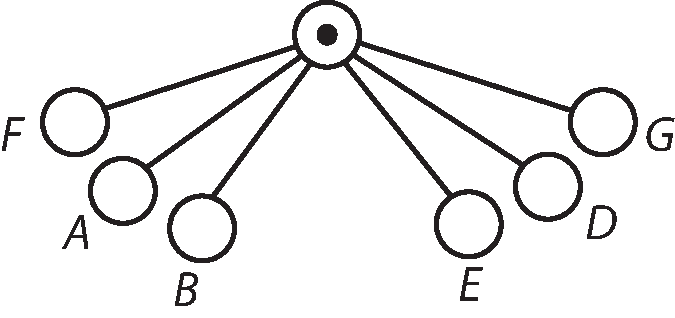
\includegraphics [trim = -3mm 3mm -13mm 0mm, clip, width=0.38\textwidth] {images/lh038_170v.pdf}
\begin{center} [\textit{Fig. 1}]\\
 \end{center}
%\caption{Bildbeschreibung}
\end{wrapfigure}
Nunc vero ponamus pendulum ex puncto \textit{A} initio libere demissum vi solius quidem gravitatis
\edtext{moveri coepisse,}{\lemma{moveri}\Bfootnote{\textbar\ facile \textit{gestr.} \textbar\ coepisse, \textit{L}}}
sed durantibus oscillationibus cum ex \textit{B} nisu
\edtext{gravitatis descendere inciperet,}%
{\lemma{gravitatis}\Bfootnote{%
\textit{(1)}\ descendens pervenisset in \textit{C} %
\textit{(2)}\ descendere inciperet, \textit{L}}}
ibi accipere ictum a rota horologii,
ac proinde majori celeritate descensum continuare quam alias fecisset
eoque motu non excurrere tantum usque ad \textit{E}, sed altius adhuc usque ad \textit{G}.
\pend 
\count\Bfootins=1050
\pstart  Porro si impetus a rota impressus non sit nimius (quod utique caveri potest ac debet) tunc utique
\edtext{assumi poterit}{\lemma{assumi poterit}\Bfootnote{\textit{erg. L}}}
alia oscillatio \textit{FG} talis, ut pendulum ex puncto \textit{F} (recte ad hoc assumto) demissum,
libere nisu gravitatis eandem collegisset celeritatem, ubi venisset in \textit{B}, quam nunc ibi
\edtext{acquisivit %
[170~v\textsuperscript{o}]
impetu rotae impresso.}{\lemma{acquisivit}\Bfootnote{%
\textit{(1)}\ partim [170~v\textsuperscript{o}] descensu a $B$ ad $C$, partim %
\textit{(2)}\ impetu rotae impresso. \textit{L}}}
Et proinde vi hujus oscillationis pendulum etiam necessario pervenisset usque
\edtext{ad \textit{G}, eadem enim vis}{\lemma{ad \textit{G},}\Bfootnote{%
\textit{(1)}\ cum eadem %
\textit{(2)}\ eadem enim \textit{L}}}
quam pendulum habet
\edtext{in \textit{B} eodemque tendens undecunque orta ipsum eodem}%
{\lemma{in \textit{B}}\Bfootnote{%
\textit{(1)}\ undecunque orta %
\textit{(a)}\ ipsum eodem %
\textit{(b)}\ eodemque tendens, %
\textit{(2)}\ eodemque [...] eodem \textit{L}}}
elevabit, nempe in \textit{G}.
Haec oscillatio \textit{FG} utique erit aequidiuturna oscillationi spontaneae \textit{BE} vel \textit{AD}.
Sed \edtext{eadem \textit{FG} diuturnior}{\lemma{eadem}\Bfootnote{%
\textit{(1)}\ longior %
\textit{(2)}\ \textit{FG} diuturnior \textit{L}}}
esset parte sui \textit{BG},
quae cum sit aequidiuturna oscillationi praesenti \textit{BG} quae ab impetu rotae
\edtext{gravitati accedente}{\lemma{gravitati accedente}\Bfootnote{\textit{erg. L}}}
orta est, sequitur oscillationem \textit{FG},
adeoque et oscillationem \textit{AD} vel \textit{BE} diuturniorem esse oscillatione
\edtext{\textit{BG}}{\lemma{\textit{BG}}\Bfootnote{\textit{erg. L}}}
orta ab impetu rotae gravitati accedente,
ac proinde oscillationes ab inaequalibus impressionibus rotarum horologii,
aut jactationum navis, aliisque hujusmodi causis reddi inaequales.
Quod demonstrandum sumseramus.
Itaque quo
\edtext{major in pendulis obtineatur aequalitas,}{\lemma{major}\Bfootnote{%
\textit{(1)}\ pendulis %
\textit{(a)}\ detur %
\textit{(b)}\ inaequalitatis %
\textit{(2)}\ in pendulis obtineatur aequalitas, \textit{L}}}
adhibendum erit praeterea artificium meum,
\edtext{quo efficitur,}{\lemma{quo}\Bfootnote{%
\textit{(1)}\ alternis %
\textit{(2)}\ efficitur, \textit{L}}}
ut impetus pendulo vel elastro, eorumve libramento impressus sit semper idem.
Machina Horologii pondus aliquod vel Elastrum exiguum, tantisper
\edtext{dum libramentum}{\lemma{dum}\Bfootnote{%
\textit{(1)}\ pendulum %
\textit{(2)}\ libramentum \textit{L}}}
vibratur restituente, ut
\edtext{postea ad rediens libramentum, novo ictu priorem aequante percutiendum sit paratum.}%
{\lemma{postea}\Bfootnote{%
\textit{(1)}\ rediens libramentum paratum %
\textit{(2)}\ ad rediens [...] paratum. \textit{L}}}
Ex his ratio redditur ejus quod ipse fatetur Hugenius,\protect\index{Namensregister}{\textso{Huygens}, Christiaan (1629-1695)}
quo minore vi pendula motum continuare possunt, eo esse exactiora;
quod non esset, si vis impressa non turbaret.\pend
\count\Bfootins=1500
 


 


 


 


%    \input{gesamttex/edit/LH038_170v.tex} %170v-text in 170r


\chapter[\scriptsize\uppercase{De horologiis communibus}]{\uppercase{De horologiis communibus}
\newline\lbrack April \textendash\ Mai 1673\rbrack}
\addcontentsline{toc}{chapter}{\thechapter\enskip De horologiis communibus \lbrack April \textendash\ Mai 1673\rbrack 
%\newline \href{http://leibnizviii.bbaw.de/Leibniz_Reihe_8/De\%2Bhorologiis\%2Bcommunibus/LH038_171r/index.html}{171r}
%\href{http://leibnizviii.bbaw.de/pdf/De\%2Bhorologiis\%2Bcommunibus/LH038_171r/LH038,_171+ra-07261.jpg}{Folio}
}
\vspace{8mm}
           
               
                \begin{ledgroupsized}[r]{120mm}
                \footnotesize 
                \pstart                
                \noindent\textbf{\"{U}berlieferung:}   
                \pend
                \end{ledgroupsized}
            
              
                             \begin{ledgroupsized}[r]{114mm}
                            \footnotesize 
                            \pstart \parindent -6mm
                            \makebox[6mm][l]{\textit{L}}Aufzeichnung: LH XXXVIII Bl. 170-171.
1 Bog. 4\textsuperscript{o}, beschnitten.
\nicefrac{1}{3} S. auf Bl.~171~r\textsuperscript{o}.
Bl.~171~v\textsuperscript{o} leer.
Bl.~170 überliefert N.~91.%?? = LH038_170 (De horologiis pendulis)
% = LH038_170r (De horologiis pendulis)
 \\Cc 2, Nr. 00 \pend
                            \end{ledgroupsized}
                %\normalsize
                \vspace*{5mm}
                \begin{ledgroup}
                \footnotesize 
                \pstart
            \noindent\footnotesize{\textbf{Datierungsgr\"{u}nde}: Das vorliegende St\"{u}ck N.~90 ist auf demselben Textträger überliefert wie das auf die Monate April bis Mai 1673 datierbare Stück N.~91.
%?? = LH038_170r (De horologiis pendulis)
Beide Aufzeichnungen handeln zudem von der Ganggenauigkeit von Pendeluhren.
Aus diesen beiden Gründen wird die Datierung von N.~91 %
auch für N.~90 %?? = vorliegendes Stück
vorgeschlagen.}
                \pend
                \end{ledgroup}
            
                \vspace*{8mm}
                \pstart 
                \normalsize
            \noindent[171~r\textsuperscript{o}]
In Horologio\protect\index{Sachverzeichnis}{horologium} communi,
pars quae Germanis vocatur inquies\protect\index{Sachverzeichnis}{inquies} impetum rotae moratur,
dum simul
\edtext{contrariis dentibus}{\lemma{contrariis}\Bfootnote{\textit{(1)}\ parte \textit{(2)}\ dentibus \textit{L}}}
illiditur;
sed quia impetus concepti pars magna perditur ea ratione;
cogitavi an non satius sit, rotam vi sua elateriolum\protect\index{Sachverzeichnis}{elaterium} tendere,
atque ita ubi ipsum ad certum perduxit terminum,
fracta vi sua impeditum
\edtext{teneri, maxima vis}{\lemma{teneri,}\Bfootnote{\textit{(1)}\ magna vis \textit{(2)}\ maxima vis \textit{L}}}
parte hoc modo conservata.
Et posset hoc Elastrum esse additum ipsi illi inquieti,
cujus dum extrema in diversa pelluntur,
posset tendi Elastrum in medio, ad certum usque terminum.
Sed pendulum staticum vel Elasticum mox reversum liberabit hoc Elaterium,
et ab eo ictum accipiet.
Quo peracto rota quoque horologii Elateriolum inquietis denuo
\edtext{tendet.
\newline%
\indent%
\hspace{-2mm}Pendulum}{\lemma{tendet.}\Bfootnote{\textit{(1)}\ In \textit{(2)}\ Pendulum \textit{L}}}
staticum \hspace{-0.15mm}affigi \hspace{-0.2mm}solet \hspace{-0.15mm}libramento,
\hspace{-0.15mm}at \hspace{-0.1mm}Elasticum \edtext{tenet \hspace{-0.15mm}arborem}{\lemma{tenet}\Bfootnote{\textit{(1)}\ arb \textit{(2)}\ in medio \textit{(3)}\ arborem \textit{L}}} \hspace{-0.15mm}rotae \hspace{-0.1mm}ser\-ra\-tae.\pend
 


 





\chapter[\scriptsize\uppercase{Sur les petites oscillations des pendules}]{\uppercase{Sur les petites oscillations des pendules}
\newline\lbrack Oktober \textendash\ November 1674\rbrack}
\addcontentsline{toc}{chapter}{\thechapter\enskip Sur les petites oscillations des pendules \lbrack Oktober \textendash\ November 1674\rbrack 
%\newline \href{http://leibnizviii.bbaw.de/Leibniz_Reihe_8/Sur\%2Bles\%2Bpetites\%2Boscillations\%2Bdes\%2Bpendules.\%2BDeuxci\%2526egrave\%253Bme\%2Bessai/LH037\%252C05_056v/index.html}{056v}
%\href{http://leibnizviii.bbaw.de/pdf/Sur\%2Bles\%2Bpetites\%2Boscillations\%2Bdes\%2Bpendules.\%2BDeuxci\%2526egrave\%253Bme\%2Bessai/LH037\%252C05_056v/LH037,05_056+va-00135.jpg}{Folio}
}
%\vspace{8mm}
    \vspace*{8mm}
\pstart 
\footnotesize
\noindent In den folgenden zwei Texten diskutiert Leibniz das Problem, wie von der Schwingungs\-zahl zweier oder mehrerer Pendel auf deren L\"{a}nge geschlossen werden kann. Die St\"{u}cke N. 17\textsubscript{1} und N. 17\textsubscript{2} geben daf\"{u}r Regeln an, die f\"{u}r unter\-schiedliche Ausgangsbedingungen gelten. Ein vergleichba\-res Problem behandelt auch N.~16.
%=LH XXXV 12, 2 Bl. 62 r = De pendulorum longitudinibus
Dass darin mit denselben Rechenbeispielen operiert wird, spricht f\"{u}r eine gemeinsame Ent\-stehungs\-zeit. Dieser Befund kann sich zudem auf \"{u}bereinstimmende Wasserzeichen  st\"{u}tzen, die für das Frühjahr 1675 belegt sind. 
Zusammen mit N. 16
%=LH XXXV 12, 2 Bl. 62 r = De pendulorum longitudinibus
ist ein in \cite{00115}\title{LSB} VII, 5 N. 9 erschienenes Stück überliefert, das auf Oktober 1674 datiert wird. 
\pend
 
 



\vspace{12mm}
\section[\scriptsize\uppercase{Sur les petites oscillations des pendules. Premier essai}]{\uppercase{Sur les petites oscillations des pendules. Premier essai}}
\addcontentsline{toc}{section}{\thesection\enskip Sur les petites oscillations des pendules. Premier essai}
\vspace{4mm}
    	\begin{ledgroupsized}[r]{120mm}
	\footnotesize 
	\pstart 
	\noindent\textbf{\"{U}berlieferung:}
	\pend
	\end{ledgroupsized}
	\begin{ledgroupsized}[r]{114mm}
	\footnotesize 
	\pstart \parindent -6mm
	\makebox[6mm][l]{\textit{L}}Aufzeichnung:
LH XXXVII 5 Bl. 56.
1 Bl. 4\textsuperscript{o}.
1\,\nicefrac{1}{5} S. auf Bl.~56~r\textsuperscript{o} und im untersten Teil von Bl.~56~v\textsuperscript{o}.
Bl.~56~v\textsuperscript{o} überliefert zudem N.~17\textsubscript{2}.
Ein Wasserzeichen, beschnitten.
Papier durch Erhaltungsma{\ss}nahmen stabilisiert.%
%	Konzept: LH XXXVII 5 Bl. 56. 1 Bl. 4\textsuperscript{o}. Papier durch Erhaltungsma{\ss}nahmen stabilisiert. 1 \nicefrac{1}{5} S.
	\\Cc 2, Nr. 975 A\pend
	\end{ledgroupsized}
	
	\count\Bfootins=1200
	\count\Afootins=1200

	
	\vspace*{8mm}
	\pstart 
	\normalsize
	\noindent[56~r\textsuperscript{o}] Deux pendules\protect\index{Sachverzeichnis}{pendule} \edtext{inegales}{\lemma{}\Bfootnote{inegales \textit{erg.} \textit{L}}} estant donn\'{e}es, et le nombre \edtext{des battements}{\lemma{nombre}\Bfootnote{\textit{(1)}\ du battement \textit{(2)}\ des battements \textit{L}}} de chacune dans un m\^{e}me temps, (: comme par exemple dans une heure :) estant connu; il faut diviser le plus grand nombre \edtext{par le moindre;}{\lemma{par le}\Bfootnote{\textit{(1)}\ nombre \textit{(2)}\ moindre; \textit{L}}} et prendre par apres le nombre quarr\'{e} du produit ou du quotient: \edtext{et autant de fois que le dit nombre}{\lemma{quotient:}\Bfootnote{\textit{(1)}\ et comme a le dit nombr \textit{(2)}\ et [...] nombre \textit{L}}} quarr\'{e} contient l'unit\'{e} autant de fois la longueur de la plus grande des deux pendules contiendra celle de la petite.
	\pend 
\pstart Par exemple si de deux pendules la plus grande fait 333 vibrations\protect\index{Sachverzeichnis}{vibration} dans \edtext{un}{\lemma{dans}\Bfootnote{\textit{(1)}\ une \textit{(2)}\ un \textit{L}}} certain espace de temps, et la moindre en \edtext{m\^{e}me}{\lemma{}\Bfootnote{m\^{e}me \textit{erg.} \textit{L}}} temps 999, divisant 999 vous \edtext{aurez 3.%
\edtext{}{\lemma{}\Afootnote{\textit{Am Rand:} $\frac{999}{333}$\vspace{-4mm}}}
dont le quarr\'{e} est 9 et par consequent}{\lemma{aurez 3.}\Bfootnote{\textit{(1)}\ et par consequent \textit{(2)}\ dont [...] consequent \textit{L}}} la raison des longueurs sera comme d'un \`{a} 9.
\pend 
\count\Bfootins=1100
\pstart
De m\^{e}me, si \edtext{la moindre}{\lemma{si}\Bfootnote{\textit{(1)}\ l'une \textit{(2)}\ la moindre \textit{L}}} fait $1500$ battements, pendant que la plus grande fait $\displaystyle1000$; divisant $\displaystyle1500$ par $\displaystyle1000$, nous aurons $1+\rule[-4mm]{0mm}{9mm}\displaystyle\frac{1}{2}$, ou reduisant tout \`{a} une fraction, nous aurons $\displaystyle\frac{3}{2}$, dont le quarr\'{e} est $\displaystyle\frac{9}{4}$, par consequent \edtext{la}{\lemma{consequent}\Bfootnote{\textit{(1)}\ une \textit{(2)}\ la \textit{L}}} moindre par exemple ayant quatre pouces la plus grande\rule[-4mm]{0mm}{9mm} en aura 9.
\pend
%\vspace{2mm}
\pstart
$\displaystyle\protect\begin{array}{lllllllll}
% Line 1
% Column 1
\protect\vspace{1mm} \displaystyle\protect\frac{34}{21} \ \protect\mbox{\protect\large f} \ \displaystyle1 +  \displaystyle\protect\frac{13}{21}\  
& % Column 2
\displaystyle\protect\frac{35}{21}\ 
& % Column 3
\displaystyle\protect\frac{\protect\overset{\protect\scriptstyle 14}{\protect\cancel{3}\protect\cancel{4}}}{\protect\cancel{2}\protect\cancel{1}} \ \protect\mbox{\protect\large f} 
& % Column 4
\displaystyle1 \displaystyle\protect\frac{14}{21}\ \lbrack \textit{sic!}\rbrack \ 
& % Column 5
& % Column 6
\hspace{9pt} \displaystyle\efrac{999}{999} 
& % Column 7
& % Column 7
& % Column 9
\hspace{6pt} \displaystyle\efrac{333}{\uline{333}} 
\\
% Line 2 
% Column 1
& % Column 2
& % Column 3
& % Column 4
1\hspace{3pt}\displaystyle\protect\frac{2}{3}\hspace{1pt} 
& % Column 5
& % Column 6
\ \displaystyle\efrac{999}{333} \ \protect\mbox{\protect\large f}\ \displaystyle\protect\frac{3}{1}
& % Column 7
&  % Column 8
\displaystyle\frac{9}{1}
& % Column 9
\hspace{3pt}\displaystyle\efrac{\ 999}{999} 
\\
% Line 3
% Column 1
& % Column 2
& % Column 3
& % Column 4
\displaystyle\protect\overline{\protect\frac{5}{3} \hspace{1pt} \protect\frac{25}{9}} 
& % Column 5
\hspace{-7pt} \displaystyle\protect\mbox{\protect\large f} \ \displaystyle2 \protect\frac{7}{9} \ \protect\frac{\protect\raisebox{0ex}{A}^2}{\protect\raisebox{0ex}{B}^2}\protect
& % Column 6
& % Column 7
& % Column 8
& % Column 9
\hspace{-3pt}\displaystyle\genfrac{}{}{}{}{999}{110889}
\end{array}$
\pend
%
%
%
\vspace*{2mm}
\pstart
\hspace{3pt}$\displaystyle1+\frac{13}{21}$ \hspace{3pt} $\displaystyle1+\frac{13}{21}$ \hspace{3pt} $\displaystyle\frac{34}{21}$ \hspace{3pt} $\displaystyle\frac{\displaystyle\genfrac{}{}{0pt}{}{13}{13}}{9}$
\pend
%
%
%
\vspace{4mm}
\pstart
$\displaystyle\protect\begin{array}[t]{llllll}
% Line 1
% Column 1
\displaystyle1+\frac{13}{21}
& % Column 1
& % Column 2
\displaystyle1\hspace{9pt}\frac{13}{21}
& % Column 3
\displaystyle\efrac{13}{\uline{13}}
\\
% Line 2
% Column 1
& % Column 2
& % Column 3
\uline{\displaystyle1\hspace{9pt}\frac{13}{21}\hspace{2pt}}
& % Column 4
\displaystyle\efrac{39}{}
\\
% Line 3
% Column 1
\displaystyle\frac{26}{42}
& % Column 2
\displaystyle\frac{169}{441}
& % Column 3
\displaystyle\frac{13}{21}\hspace{3pt}\frac{169}{441}
& % Column 4
\displaystyle\frac{13}{\uline{169}}
& % Column 5
\hspace{3pt}\displaystyle\efrac{21}{\uline{21}}
\\
% Line 4
% Column 1
& % Column 2
& % Column 3
\uline{\displaystyle\frac{13}{21}\hspace{12pt}}
& % Column 4
& % Column 5
\displaystyle\efrac{\hspace{3pt}21}{\hspace{-3pt}\uline{42}}
\\
% Line 5
% Column 1
& % Column 2
& % Column 3
& % Column 4
& % Column 5
\displaystyle\efrac{441}{}
\end{array}$
\pend
%
%
%
%\count\Bfootins=1500
%\vspace{4mm}
%\newpage
\pstart\noindent
[56~v\textsuperscript{o}] \hspace*{4mm}\lbrack \textit{Quer zur Schreibrichtung:}\rbrack 
\pend 
%
%
%
\vspace{2mm}
\pstart\noindent
La moindre $1500$:
\pend
%
%
%
\pstart\noindent
La plus grande $1000$
\pend
%
%
%
\vspace*{2mm}
\pstart\noindent
\begin{tabular}{c}
\cancel{1500}
\\
\cancel{1000}
\\
\end{tabular}
$\displaystyle \bigg \vert \frac{3}{2}$
\pend
%
%
%
\vspace{2mm}
\pstart\noindent
\hspace*{1mm}
$\displaystyle \frac{3}{2}$
\begin{tabular}{c}
\textemdash
\\
\textemdash
\\
\end{tabular}
$\displaystyle \frac{3}{2}$ \hspace*{5mm} $\displaystyle \frac{9}{4}$
\pend
%
%
%
\pstart\noindent
\vspace{2mm}
\hspace{4mm}
$\displaystyle 2\ \frac{1}{4}$
\pend
\count\Bfootins=1500
\count\Afootins=1500
\newpage


	 
	

\vspace{4mm}
\section[\scriptsize\uppercase{Sur les petites oscillations des pendules. Deuxi\`{e}me essai}]{\uppercase{Sur les petites oscillations des pendules. Deuxi\`{e}me essai}}
\addcontentsline{toc}{section}{\thesection\enskip Sur les petites oscillations des pendules. Deuxi\`{e}me essai}
\vspace{4mm}
    \begin{ledgroupsized}[r]{120mm}
\footnotesize 
\pstart 
\noindent\textbf{\"{U}berlieferung:}
\pend
\end{ledgroupsized}

\begin{ledgroupsized}[r]{114mm}
\footnotesize 
\pstart \parindent -6mm
\makebox[6mm][l]{\textit{L}}Aufzeichnung:
LH XXXVII 5 Bl. 56.
1 Bl. 4\textsuperscript{o}.
\nicefrac{4}{5} S. auf Bl.~56~v\textsuperscript{o}.
Bl. 56~r\textsuperscript{o} und das unterste Fünftel von Bl. 56~v\textsuperscript{o} überliefern N.~17\textsubscript{1}.
% = LH037_05_056v (Sur les petites 1)
Ein Wasserzeichen, beschnitten.
Papier durch Erhaltungsma{\ss}nahmen stabilisiert.%
\newline%
Cc 2, Nr. 975 B%
%%Konzept: LH XXXVII 5 Bl. 56. 1 Bl. 4\textsuperscript{o}. Papier durch Erhaltungsma{\ss}nahmen stabilisiert. \nicefrac{4}{5} S. auf Bl. 56~v\textsuperscript{o}. Auf Bl. 56~r\textsuperscript{o} und \nicefrac{1}{5} S. auf Bl. 56~v\textsuperscript{o} das St\"{u}ck N. ??
%% = LH037_05_056v (Sur les petites 1)
%\\Cc 2, Nr. 975B
\pend
\end{ledgroupsized}
%%\normalsize
%\vspace*{5mm}
%\begin{ledgroup}
%\footnotesize
%\pstart
%\noindent\footnotesize{\textbf{Datierungsgr\"{u}nde}: Siehe oben die Einleitung zu N. ??Intro??.}
%\pend
%\end{ledgroup}

\count\Bfootins=1200
	\count\Afootins=1200
\vspace*{8mm}
\pstart\normalsize\noindent%
[56~v\textsuperscript{o}]
% \selectlanguage{french}
Si vous demandez la longueur d'un pendule,\protect\index{Sachverzeichnis}{pendule}
qui fasse un certain nombre de batte\-ments dans un certain temps,
\edtext{par exemple dans un quart d'heure;}{\lemma{par [...] d'heure}\Bfootnote{\textit{erg. L}}}
vous la pourrez trouver ainsi:%
\pend%
\pstart %
Prenez
\edtext{une pendule,}{\lemma{une}\Bfootnote{\textit{(1)}\ autre pendule, dont \textit{(2)}\ pendule, \textit{L}}}
\`{a} discretion, mesurez sa longueur; et contez combien de batte\-ments elle fait dans le m\^{e}me temps susdit, par exemple dans un quart d'heure.
\pend% 
\pstart%
A present pour s'expliquer plus aisement, appellons le nombre des battements de  la pendule, prise \`{a} discretion, \textit{$(A)$} et le nombre des battements  demand\'{e}, de la pendule dont nous cherchons la longueur, \textit{$(B)$}  et la longueur de la pendule prise \`{a} discretion, \textit{$(C)$}  et enfin la longueur de la pendule demand\'{e}e, \textit{$(D)$}.
Cela estant pos\'{e}, l'operation sera telle.
\pend%
\vspace*{2.0em}%
\pstart\noindent%
\lbrack%
\textit{Nachfolgend klein gedruckter Text gestrichen:}%
\rbrack %
\pend%
\vspace*{0.5em}
\pstart\noindent\footnotesize%
Des deux nombres, $(A)$ et $(B)$ divisez le plus grand par le moindre;
et multipliez le quotient par luy m\^{e}me, ou (ce qui est  la m\^{e}me chose) prenez le quarr\'{e} du dit quotient:
appellons le dit quarr\'{e}, $(E)$.%
\pend%
\pstart\footnotesize%
Enfin faites l'operation suivante de la regle des
\edtext{trois;%
\newline%
Si le nombre quarr\'{e} $(E)$,}{\lemma{trois;}\Bfootnote{%
\textit{(1)}\ Comme le nombre quarr\'{e} $F$, %
\textit{(2)}\ Si le nombre quarr\'{e} $(E)$ \textit{L}}}
donne l'Unit\'{e}; combien%
\pend%
\vspace*{1mm}%
\pstart\footnotesize%
$\displaystyle\frac{A}{B}$\hspace*{2mm}$\displaystyle\frac{A^{2}}{\underline{\underline{{B}^{2}}}}$\hspace*{2mm}$\displaystyle\frac{C}{D}$
\pend%
\pstart%
\vspace{0,8mm}\hspace*{6mm}$r$
\pend%
\vspace*{1.5em}%
\pstart\normalsize\noindent%
Multipliez le nombre $A$ par luy m\^{e}me, ou (:~ce qui est la m\^{e}me chose~:) prenez son quarr\'{e};
de m\^{e}me multipliez le nombre $B$ par luy m\^{e}me, ou prenez son quarr\'{e};
et enfin faites une telle operation de la regle des trois:
\pend%
\newpage%
\pstart%
\edtext{Si le quarr\'{e} du nombre $A$ des battements}{\lemma{Si le}\Bfootnote{%
\textit{(1)}\ nombre %
\textit{(2)}\ quarr\'{e} du nombre %
\textit{(a)} des battements $A$ %
\textit{(b)}\ $A$ des battements \textit{L}}}
de la pendule prise \`{a} discretion, donne la longueur $C$, de sa pendule.
\pend%
\pstart%
Combien donnera le quarr\'{e} du Nombre
\edtext{donn\'{e}}{\lemma{donn\'{e}}\Bfootnote{\textit{erg. L}}}
$B$ des battements de la pendule demand\'{e}e,
pour la longueur $D$, de la dite pendule.
\pend%
\pstart%
Et le produit de cette operation, vous donnera la dite longueur $D$, que vous aviez demand\'{e}e.
\selectlanguage{latin}
\pend
\count\Bfootins=1500
	\count\Afootins=1500




\chapter[\scriptsize\uppercase{De pendulorum longitudinibus}]{\uppercase{De pendulorum longitudinibus}
\newline\lbrack Oktober \textendash\ November 1674\rbrack}
\addcontentsline{toc}{chapter}{\thechapter\enskip De pendulorum longitudinibus \lbrack Oktober \textendash\ November 1674\rbrack}
\vspace{8mm}
          
               
                \begin{ledgroupsized}[r]{120mm}
                \footnotesize 
                \pstart                
                \noindent\textbf{\"{U}berlieferung:}   
                \pend
                \end{ledgroupsized}
            
              
                            \begin{ledgroupsized}[r]{114mm}
                            \footnotesize 
                            \pstart \parindent -6mm
                            \makebox[6mm][l]{\textit{L}}Notiz: LH XXXV 12, 2 Bl. 62. 1 Bl. 4\textsuperscript{o}. \nicefrac{1}{2} S. auf Bl.~62~r\textsuperscript{o}. In der unteren Hälfte von Bl.~62~r\textsuperscript{o} Rechnungen, die in \textit{LSB} VII,~3 N.~38\textsubscript{16} ediert sind; Bl.~62~v\textsuperscript{o} überliefert das Stück \textit{LSB} VII,~5 N.~9. Ein Wasserzeichen, beschnitten. Papier durch Erhaltungsmaßnahmen stabilisiert.%
\newline%
Cc 2, Nr. 543 (tlw.)%
\pend%
%                            Konzept: LH XXXV 12, 2 Bl. 62. 1 Bl. 4\textsuperscript{o}. Papier durch Erhaltungs\-ma{\ss}nahmen stabilisiert. \nicefrac{1}{2} S. auf Bl. 62~r\textsuperscript{o}. Wasserzeichen beschnitten. In der unteren Hälfte von Bl. 62~r\textsuperscript{o} Rechnungen, die in \cite{00115}\title{LSB} VII, 3 N. 38.16 ediert sind; Bl. 62~v\textsuperscript{o} enthält das Stück \cite{00115}\title{LSB} VII, 5 N. 9.\\Cc 2, Nr. 543 \pend
                            \end{ledgroupsized}
                %\normalsize
                \vspace*{5mm}
                \begin{ledgroup}
                \footnotesize 
                \pstart
            \noindent\footnotesize{\textbf{Datierungsgr\"{u}nde}: Die Datierung des St\"{u}ckes folgt derjenigen, die f\"{u}r \title[115]{LSB} VII, 5 N. 9 geliefert wird, und der dort geäußerten Vermutung, dass Leibniz zuerst die mathematischen Aufzeich\-nungen auf der R\"{u}ckseite von Bl. 62 verfasst habe. Das vorliegende St\"{u}ck k\"{o}nnte daher gleichfalls im Oktober 1674 oder in den folgenden Monaten entstanden sein, wie das Wasserzeichen nahelegt.}
                \pend
                \end{ledgroup}
            
                \vspace*{8mm}
                \pstart 
                \normalsize
            \noindent[62~r\textsuperscript{o}]  Pendulorum longitudines duplicatam habent rationem temporum, quibus minimae vibrationes\protect\index{Sachverzeichnis}{vibratio} perficiuntur.\pend \pstart \vspace{2em} \noindent
\begin{minipage}[t]{0.33\textwidth}
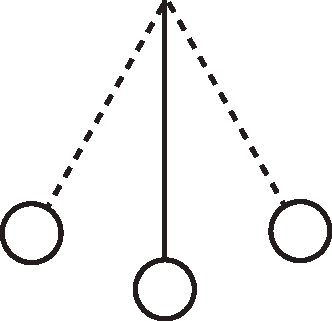
\includegraphics[width=0.6\textwidth]{images/62-1.pdf}
\end{minipage}
\hspace*{13,3mm}
\begin{minipage}[t]{0.33\textwidth}
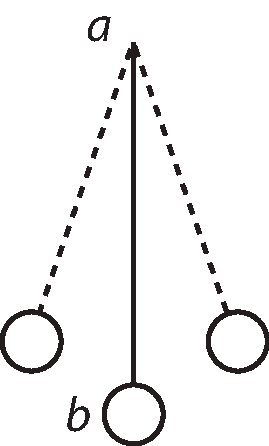
\includegraphics[width=0.47\textwidth]{images/62-2.pdf}
\end{minipage}
\hspace*{13,3mm}
\begin{minipage}[t]{0.33\textwidth}

\includegraphics[width=0.18\textwidth]{images/62_3.pdf}
\end{minipage}

%\begin{center}                    
            %   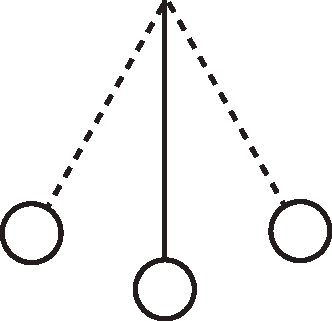
\includegraphics[width=0.55\textwidth]{images/62-1.pdf}
             %  \end{center}
               \vspace*{1mm}
                    \hspace*{-1,5mm}  [\textit{Fig. 1}]\hspace*{44mm}  [\textit{Fig. 2}] \hspace*{38mm}  [\textit{Fig. 3, gestr.}]
\vspace*{1em}                       
                        %@ @ @ Dies ist eine Abstandszeile - fuer den Fall, dass mehrere figures hintereinander kommen, ohne dass dazwischen laengerer Text steht. Dies kann zu einer Fahlermeldung fuehren. @ @ @ \\
                   
                    \vspace{2em} \noindent \setline{13}\lbrack \textit{Rechnungsfragmente ohne Textbezug:}\rbrack \pend
\vspace{1em}
                     \pstart \noindent 
 \begin{tabular}{c}
                                   1500\\
                                   1000\\
                                  \end{tabular}
                        %@ @ @ Dies ist eine Abstandszeile - fuer den Fall, dass mehrere figures hintereinander kommen, ohne dass dazwischen laengerer Text steht. Dies kann zu einer Fahlermeldung fuehren. @ @ @ \\
                    \begin{tabular}{cc}
                                  999 &333\\
                                 \end{tabular}
                        %@ @ @ Dies ist eine Abstandszeile - fuer den Fall, dass mehrere figures hintereinander kommen, ohne dass dazwischen laengerer Text steht. Dies kann zu einer Fahlermeldung fuehren. @ @ @ \\
                     \pend 
 


 


 


 


 


%    \input{gesamttex/edit/LH035_12_02_062v.tex} %v-text in R.VII


% HOROLOGIUM VENTANEUM (PR)

 \chapter[\scriptsize\uppercase{Horologium ventaneum perpetuum}]{\uppercase{Horologium ventaneum perpetuum}
 \newline\lbrack Ende 1674 ???\rbrack}
 \addcontentsline{toc}{chapter}{\thechapter\enskip Horologium ventaneum perpetuum \lbrack Ende 1674 ???\rbrack}
 \vspace{8mm}
    \begin{ledgroupsized}[r]{120mm}
\footnotesize 
\pstart
\noindent
\textbf{\"{U}berlieferung:}
\pend
\end{ledgroupsized}
\begin{ledgroupsized}[r]{114mm}
\footnotesize 
\pstart
\parindent -6mm
\makebox[6mm][l]{\textit{L}}Konzept: LH XXXVII 5 Bl. 92-93. 2 Bl. (ursprünglich 1 Bog.) 2\textsuperscript{o}. 3 S. Bl. 93~v\textsuperscript{o} leer. Kleine Textverluste durch Papierabbruch am oberen Rand von Bl. 92~v\textsuperscript{o} und 93~r\textsuperscript{o}. Beide Blätter durch Papiererhaltungsmaßnahmen gesichert. Wasserzeichen. \\Cc 2, Nr.  838
\pend
\end{ledgroupsized}
%
%\normalsize
\vspace*{5mm}
\begin{ledgroup}
\footnotesize 
\pstart
\noindent
\footnotesize{\textbf{Datierungsgr\"{u}nde}: Das Wasserzeichen ist für die Zeit von Anfang 1674 bis Anfang 1675 belegt.}
\pend
\end{ledgroup}
%
\vspace*{8mm}
\count\Bfootins=1400
\pstart
\noindent
[92~r\textsuperscript{o}]
\pend
\pstart 
\normalsize
\centering % PR: Bitte, als Überscrift formattieren.
Motus regularis continuus
a causa irregulari, discontinuata\\
seu Horologium Ventaneum\protect\index{Sachverzeichnis}{horologium ventaneum} perpetuum
\pend
\vspace*{0.5em}
\pstart
\noindent
Inter causas moventes irregulares, discontinuatas nulla est tempore crebrior, loco
\edtext{universalior, viribus\protect\index{Sachverzeichnis}{vis}}{\lemma{universalior,}\Bfootnote{\textit{(1)}\ effectu \textit{(2)}\ viribus \textit{L}}}
Efficacior Vento.\protect\index{Sachverzeichnis}{ventus}
\pend
\pstart
Supponamus ergo singulis minimum mensibus semel flare ventum.
Quanquam enim singulae septimanae sint suffecturae,
securitatis tamen majoris causa menses assumemus.
Deinde cogitemus Ventum utcunque debilem futurum esse efficacem ad rotam\protect\index{Sachverzeichnis}{rota} aliquam circumagendam
\edtext{levandumque aliquod pondus\protect\index{Sachverzeichnis}{pondus} insigne; tempore Mensis}{\lemma{}\Bfootnote{levandumque [...] Mensis \textit{erg. L}}}
duas ob \edtext{causas,\\
\hspace*{7,5mm}\textso{primo }quanto impulsus\protect\index{Sachverzeichnis}{impulsus} ad eundem effectum tendentes sunt magis multiplicati. Possumus enim ex omnibus partibus excipere impulsum venti ad vires lucrandas[;]\\
\hspace*{7,5mm}\textso{secundo }quanto longius tempus in elevandum pondus impenditur.
Ventus\protect\index{Sachverzeichnis}{ventus} enim aut diu durat, aut saltem crebro redit, intra spatium unius mensis.}{\lemma{causas,}\Bfootnote{\textit{(1)}\ \textso{primum} ob 
\textit{(2)}\ \textso{primo} quanto pinnae\protect\index{Sachverzeichnis}{pinna} seu extremitates rotae\protect\index{Sachverzeichnis}{rota} sunt a centro remotiores \textso{secundo} quanto impulsus\protect\index{Sachverzeichnis}{impulsus} ad eundem effectum\protect\index{Sachverzeichnis}{effectus} tendentes sunt magis multiplicati \textso{tertio} quanto longius tempus in elevandum pondus\protect\index{Sachverzeichnis}{pondus} impenditur.
\textit{(3)}\ \textso{primo} [...] mensis.
\textit{L}}}
\pend
%\newpage
\count\Bfootins=1400
\pstart
Denique \edtext{supponamus Horologium\protect\index{Sachverzeichnis}{horologium} nobis esse aliudve Automaton\protect\index{Sachverzeichnis}{automaton}}{\lemma{supponamus}\Bfootnote{\textit{(1)}\ Horologium nobis esse, aliamve Ma
\textit{(2)}\  Horologium [...] Automaton
\textit{L}}}
quod integro Mense decurrere possit,
antequam renovatione seu red-elevatione ponderum\protect\index{Sachverzeichnis}{pondus} opus habeat.
Hoc fieri potest duobus
\edtext{modis,\\
\hspace*{7,5mm}\textso{primo}}{\lemma{modis,}\Bfootnote{\textit{(1)}\ primum
\textit{(2)}\ \textso{primo}}}\textso{
}si \edtext{Pondus\protect\index{Sachverzeichnis}{pondus} movens satis profunde}{\lemma{Pondus}\Bfootnote{\textit{(1)}\ satis 
\textit{(a)}\ alte
\textit{(b)}\ prof
\textit{(2)}\ movens satis profunde
\textit{L}}}
descendere possit, ut in turri praealta.
\edtext{Pone longissimum funem esse circa cylindrum aliquem replicatum,
Pondusque\protect\index{Sachverzeichnis}{pondus} funi appensum, descendendo, Cylindrum circumagere[;]}{\lemma{}\Bfootnote{Pone [...] circumagere \textit{erg. L}}}\\
\hspace*{7,5mm}\textso{secundo }si ponderis impetus\protect\index{Sachverzeichnis}{impetus}
rotis\protect\index{Sachverzeichnis}{rota} multiplicatis tardetur, ita enim fieri poterit,
ut longo tempore per exiguum spatium descendat ingens licet pondus.
\pend
\pstart
His ita positis fiet ut pondus\protect\index{Sachverzeichnis}{pondus} Horologii\protect\index{Sachverzeichnis}{horologium} ante Mensis decursum a Vento\protect\index{Sachverzeichnis}{ventus} red-elevetur in altitudinem priorem.\textso{
Ita }\edtext{\textso{habemus Effectum continuum a causa}}{\lemma{\textso{habemus}}\Bfootnote{\textit{(1)}\ \textso{a causa}
\textit{(2)}\ \textso{Effectum} [...] \textso{causa}
\textit{L}}}\textso{
discontinuata.}\edtext{ Unde habebimus \textso{Molendinum Ventaneum}\protect\index{Sachverzeichnis}{molendinum ventaneum}\textso{ perpetuum
}quod vento etiam non flante circumagatur.}{\lemma{}\Bfootnote{Unde [...] circumagatur. \textit{erg. L}}}\textso{
}\edtext{\textso{Restat ut ex causa irregulari impetremus Effectum regularem.}}{\lemma{}\Bfootnote{\textso{Restat} [...] \textso{regularem.} \textit{erg. L}}}
\pend
\pstart
\textso{Obstaculum }est irregularitas ab hoc motu venti
\edtext{metuenda}{\lemma{}\Bfootnote{metuenda \textit{erg. L}}},
quo enim momento ventus\protect\index{Sachverzeichnis}{ventus} elevat pondus,\protect\index{Sachverzeichnis}{pondus}
eo tempore Pondus horologium non gravabit.
Horologium\protect\index{Sachverzeichnis}{horologium} ergo interquiescet,
ac proinde motus ejus erit irregularis.
\pend
\pstart
\textso{Remedium }obstaculi hujus utique maximi ad successum momenti est,
alioqui enim impossibile
\edtext{est ex irregulari causa}{\lemma{est}\Bfootnote{\textit{(1)}\ Ex causa
\textit{(2)}\ ex irregulari causa
\textit{L}}}
effectum impetrare Regularem.
Id ergo inveni tandem, certissimum, facillimumque, nisi fallor.
Sunto nimirum duo pondera\protect\index{Sachverzeichnis}{pondus}
\edtext{aequalia}{\lemma{aequalia}\Bfootnote{\textit{erg. L}}}
quae alternis horologium\protect\index{Sachverzeichnis}{horologium} gravent;
ut quando unum a vento\protect\index{Sachverzeichnis}{ventus} red-elevatur, alterum interea liberatum
\edtext{ab obstaculo}{\lemma{ab obstaculo}\Bfootnote{\textit{erg. L}}}
horologii motum faciat continuari,
sed in idem obstaculum recidat,
ubi \edtext{primum prius}{\lemma{primum}\Bfootnote{\textit{(1)}\ alterum
\textit{(2)}\ prius
\textit{L}}}
elevari desinit.
\pend
\pstart
Ex his fundamentis Machinam\protect\index{Sachverzeichnis}{machina} formare non difficile est,
cujus haec erit\textso{ Constructio:\protect\index{Sachverzeichnis}{constructio}}
[92~v\textsuperscript{o}]
\pend
\newpage
\count\Bfootins=1200
\pstart
\noindent
    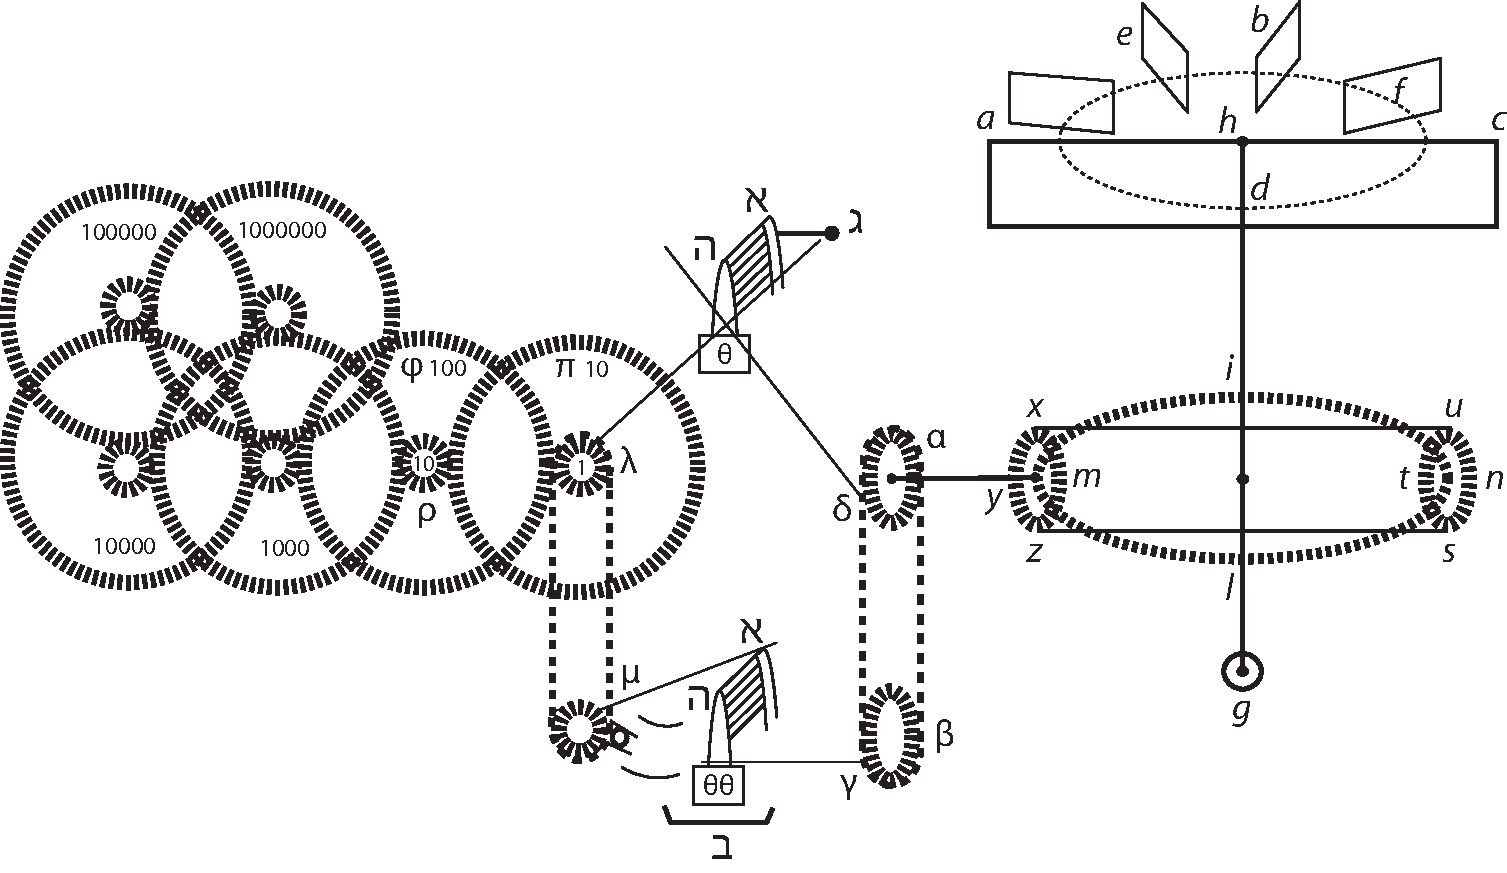
\includegraphics[width=1.0\textwidth]{images/LH037,05_092v-d1.pdf}\\
%\vspace{-4mm}
\begin{center}
  [\textit{Fig. 1}] 
  \end{center}\edtext{}{\lemma{\hspace{2mm}[\textit{Fig. 1}]}\killnumber\Cfootnote{Am unteren Ende der Kette $\displaystyle \alpha\beta\gamma\delta$ ist im Ms. ein zweites, hier nicht abgebildetes $\displaystyle \beta$ gezeichnet.}} 
  \pend
\pstart
\centering
Horologium \setline{1}Ventaneum\protect\index{Sachverzeichnis}{horologium ventaneum} perpetuum. 
\pend
\pstart
\noindent
Esto Rota\protect\index{Sachverzeichnis}{rota} Horizonti parallela $\displaystyle abcd$ semitecta et
\edtext{semiaperta, latus apertum $\displaystyle abc$. latus tectum}{\lemma{semiaperta,}\Bfootnote{\textit{(1)}\ pars tecta
\textit{(2)}\ latus
\textit{(a)}\ tectum
\textit{(b)}\ apertum [...] tectum
\textit{L}}}
\edtext{$\displaystyle adc$. Circumferentiae ejus
alae\protect\index{Sachverzeichnis}{ala}}{\lemma{$\displaystyle adc$.}\Bfootnote{\textit{(1)}\ alae in rota
\textit{(2)}\ Circumferentiae ejus alae
\textit{L}}}
infixae sunt
\edtext{$\displaystyle a$. $\displaystyle e$. $\displaystyle b$. $\displaystyle f$. $\displaystyle c$. etc.}{\lemma{}\Bfootnote{$\displaystyle a$. $\displaystyle e$. [...] etc.
\textit{ erg. L}}},
quae a vento\protect\index{Sachverzeichnis}{ventus} circumaguntur.
Ponatur enim $\displaystyle c$ esse oriens, $\displaystyle a$ occidens, $\displaystyle b$ septentrio, $\displaystyle d$ meridies.
Ventus orientalis $\displaystyle b$ aget versus $\displaystyle e$. occidentalis $\displaystyle b$ aget versus $\displaystyle f$. septentrionalis $\displaystyle a$ versus $\displaystyle d$. meridionalis $\displaystyle a$ versus $\displaystyle e$.
Eademque de caeteris ventis intermediis ratio est.
Ala\protect\index{Sachverzeichnis}{ala} autem $\displaystyle a$ eunte versus $\displaystyle e$. aut ala $\displaystyle f$ versus $\displaystyle b$.
alia ala ex latere tecto prodiens
\edtext{in ejus}{\lemma{in}\Bfootnote{\textit{(1)}\ earum
\textit{(2)}\ ejus
\textit{L}}}
locum succedit.
\pend
\pstart
Cur autem alterum latus tectum sit[,]
 ratio est ne ventus\protect\index{Sachverzeichnis}{ventus}
\edtext{in oppositas alas\protect\index{Sachverzeichnis}{ala} simul incidens}{\lemma{in}\Bfootnote{\textit{(1)}\ ejus alas incidens, vento
\textit{(2)}\ oppositas [...] incidens,
\textit{L}}},
sibi reluctetur.
Ut si ventus\protect\index{Sachverzeichnis}{ventus} septentrionalis a $\displaystyle b$ versus $\displaystyle d$ simul in alam\protect\index{Sachverzeichnis}{ala} $\displaystyle a$ et in oppositam $\displaystyle c$ incidat,
fiet aequilibrium, nec ratio erit cur huc potius quam illuc rota\protect\index{Sachverzeichnis}{rota} agatur[;]
\edtext{quemadmodum molendina aquatica\protect\index{Sachverzeichnis}{molendinum aquaticum} aquae immerguntur, nisi parte tantum, alioqui cursu ejus non circumagerentur, nisi debiliter, quod miror in
molendinis\protect\index{Sachverzeichnis}{molendinum} vulgaribus non observatum}{\lemma{}\Bfootnote{quemadmodum molendina aquatica\ \textbar\
\textit{(1)}\ in aquae libere po
\textit{(2)}\ in aquam
\textit{(3)}\ aquae\ \textbar\
immerguntur, [...] observatum
\textit{erg. L}}}.
\pend
\pstart
\edtext{Est ergo}{\lemma{Est ergo}\Bfootnote{\textit{erg. L}}}
Rota ventanea\protect\index{Sachverzeichnis}{rota ventanea} $\displaystyle abcd$ ita
\edtext{constructa ut quolibet vento\protect\index{Sachverzeichnis}{ventus} flante continue circumagatur}{\lemma{constructa}\Bfootnote{\textit{(1)}\ quolibet vento continue circumagetur
\textit{(2)}\ ut [...] circumagatur.
\textit{L}}}.
In quo differt ab Anemoscopio\protect\index{Sachverzeichnis}{anemoscopium},
aedibus imposito aut Gnomone ventaneo,\protect\index{Sachverzeichnis}{gnomon ventaneum}
quae a praesente vento moventur non nisi semel,
quando scilicet in lineam venti,\protect\index{Sachverzeichnis}{ventus} quo minus
\edtext{ei obstent, disponantur.}{\lemma{ei}\Bfootnote{\textit{(1)}\ obstet, disponatur
\textit{(2)}\ obstent, disponantur.
\textit{L}}}
\pend
\count\Bfootins=1000
\pstart
\begin{wrapfigure}[7]{l}{0.15\textwidth}
\vspace{-5mm}
     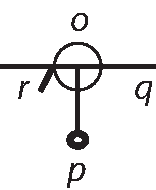
\includegraphics[trim = 0mm -3mm -5mm 0mm, clip, width=0.15\textwidth]{images/LH037,05_092v-d2.pdf}
     \centering
     [\textit{Fig. 2}] % \caption{Bildbeschreibung}
\end{wrapfigure}
Hujus Rotae ventaneae\protect\index{Sachverzeichnis}{rota ventanea} axis esto $\displaystyle gh$ mobilis cum rota $\displaystyle abcd$ in centro $\displaystyle g$ secumque movens rotam dentatam\protect\index{Sachverzeichnis}{rota dentata} $\displaystyle ilmn$ cui
\edtext{incumbit cylinder $\displaystyle mn$ desinens utrinque}{\lemma{incumbit}\Bfootnote{\textit{(1)}\ utrinque
\textit{(2)}\ cylinder [...] utrinque
\textit{L}}}
in tympana\protect\index{Sachverzeichnis}{tympanum}
\edtext{dentata $\displaystyle m$ et $\displaystyle n$ rotae\protect\index{Sachverzeichnis}{rota dentata}}{\lemma{dentata}\Bfootnote{\textit{(1)}\ $\displaystyle mn$
\textit{(2)}\ $\displaystyle m$ et $\displaystyle n$\
\textbar\ utrinque \textit{gestr.}\ \textbar\
rotae \textit{L}}}
extremitatibus incumbentia.
Horum tympanorum\protect\index{Sachverzeichnis}{tympanum} dentes\protect\index{Sachverzeichnis}{dens} ita comparati esse debent,
ut non nisi in unam partem cedant,
ubi autem cesserint et dentes rotae\protect\index{Sachverzeichnis}{rota dentata} praetermiserint,
se rursus erigant.
Exempli gratia dens\protect\index{Sachverzeichnis}{dens}
\edtext{$\displaystyle op$ circa centrum}{\lemma{$\displaystyle op$}\Bfootnote{%
\textit{(1)}\ infixus centr
\textit{(2)}\ circa centrum
\textit{L}}}
$\displaystyle o$ mobilis est solum versus $\displaystyle q$
non versus $\displaystyle r$ ob obstaculum $\displaystyle r$.
et si moveatur ab aliqua vi versus $\displaystyle q$.
ea discedente propria gravitate\protect\index{Sachverzeichnis}{gravitas} in $\displaystyle p$ appensa redit in situm priorem
%\begin{wrapfigure}[7]{l}{0.15\textwidth}
%\vspace{-5mm}
%     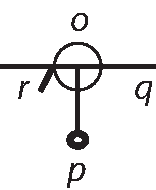
\includegraphics[trim = 0mm -3mm -5mm 0mm, clip, width=0.15\textwidth]{images/LH037,05_092v-d2.pdf}
%     \centering
%     [\textit{Fig. 2}] % \caption{Bildbeschreibung}
%\end{wrapfigure}
\edtext{perpendicularem. Ergo ponamus}{\lemma{perpendicularem.}\Bfootnote{%
\textit{(1)}\ Ergo unius Tympani,\protect\index{Sachverzeichnis}{tympanum} nempe $\displaystyle m$. dentes\protect\index{Sachverzeichnis}{dens} non sint mobiles nisi
\textit{(2)}\ Ergo ponamus
\textit{L}}}
ventum\protect\index{Sachverzeichnis}{ventus} [occidentalem]\edtext{}{\Bfootnote{occidenlatem \textit{\ L \"{a}ndert Hrsg.}}} agere rotam\protect\index{Sachverzeichnis}{rota alata}
\edtext{alatam}{\lemma{}\Bfootnote{alatam
\textit{erg. L}}}
hoc ordine $\displaystyle bcda$. aget dentatam\protect\index{Sachverzeichnis}{rota dentata} hoc ordine
\edtext{$\displaystyle inlm$. $\displaystyle i$ tendens}{\lemma{$\displaystyle inlm$.}\Bfootnote{%
\textit{(1)}\ Ergo
\textit{(2)}\ $\displaystyle i$ tendens
\textit{L}}}
per $\displaystyle n$ in $\displaystyle l$ non impediatur dentibus\protect\index{Sachverzeichnis}{dens} tympani\protect\index{Sachverzeichnis}{tympanum} horizontaliter incumbentis in $\displaystyle n$.
\edtext{quippe non cedentibus}{\lemma{quippe}\Bfootnote{%
\textit{(1)}\ mobilibus
\textit{(2)}\ non cedentibus
\textit{L}}}
ordine $\displaystyle nstu$
\edtext{seu sursum per latus meridionale quo nunc tendit rota dentata\protect\index{Sachverzeichnis}{rota dentata}, nisi cum toto cylindro sed serie $\displaystyle nuts$ seu sursum per latus septentrionale}{\lemma{}\Bfootnote{seu sursum
\textit{(1)}\ versus
\textit{(2)}\ per latus meridionale 
\textit{(a)}\ non vero serie $\displaystyle nuts $ seu sursum per latus septentrionale quo nunc impellit rota dentata\protect\index{Sachverzeichnis}{rota dentata} nisi cum toto cylindro
\textit{(b)}\ quo
\textit{(aa)}\ tendit
\textit{(bb)}\ nunc impellit rota dentata
\textit{(c)}\ quo nunc [...] septentrionale.
\textit{erg. L}}}.
At eodem motu $\displaystyle l$ tendens per $\displaystyle m$ in $\displaystyle i$ non impedietur dentibus\protect\index{Sachverzeichnis}{dens} tympani\protect\index{Sachverzeichnis}{tympanum} horizontaliter incumbentis in $\displaystyle m$.
\edtext{quippe itidem cedentibus sine toto cylindro}{\lemma{quippe}\Bfootnote{%
\textit{(1)}\ itidem mobilibus tantum serie
\textit{(2)}\ itidem 
\textit{(a)}\ serie non mobilibus
\textit{(b)}\ cedentibus [...] cylindro
\textit{L}}}
sursum per latus septentrionale seu serie
\edtext{$\displaystyle mxyz$ quo nunc tendit rota dentata,\protect\index{Sachverzeichnis}{rota dentata}\textso{ sine toto cylindro }non vero sursum}{\lemma{$\displaystyle mxyz$}\Bfootnote{%
\textit{(1)}\ quo parte nunc tendit rota, \textso{nisi cum toto cylindro}
\textit{(2)}\ quo nunc [...] \textso{cylindro}
\textit{(a)}\ sed tantum deorsum
\textit{(b)}\ non vero sursum
\textit{L}}}
per latus meridionale seu serie $\displaystyle mzyx$
\edtext{nisi cum toto cylindro}{\lemma{}\Bfootnote{%
nisi [...] cylindro
\textit{ erg. L}}}.
Ergo Cylinder circumagetur sursum in
\edtext{latus meridionale}{\lemma{latus}\Bfootnote{%
\textit{(1)}\ septentrionale
\textit{(2)}\ meridionale
\textit{L}}}
serie $\displaystyle nstu$ seu $\displaystyle mzyx$. Contra ponatur vento\protect\index{Sachverzeichnis}{ventus} verso Rota alata\protect\index{Sachverzeichnis}{rota alata} verti
[93~r\textsuperscript{o}]
ordine $\displaystyle badc$ et rota dentata\protect\index{Sachverzeichnis}{rota dentata}
\edtext{serie $\displaystyle imln$.}{\lemma{serie}\Bfootnote{%
\textit{(1)}\ $\displaystyle lnim$.
\textit{(2)}\ $\displaystyle imln$.
\textit{L}}}
\edtext{$\displaystyle i$ tendens}{\lemma{$\displaystyle i$}\Bfootnote{%
\textit{(1)}\ veniens
\textit{(2)}\ tendens
\textit{L}}}
per $\displaystyle m$ versus $\displaystyle l$ dentibus\protect\index{Sachverzeichnis}{dens} Tympani\protect\index{Sachverzeichnis}{tympanum} in $\displaystyle m$. quippe
versus \edtext{$\displaystyle z$. non cedentibus nisi cum cylindro tenebitur;
at $\displaystyle l$ tendens per $\displaystyle n$ in $\displaystyle i$ non tenebitur dentibus\protect\index{Sachverzeichnis}{dens} tympani\protect\index{Sachverzeichnis}{tympanum} in $\displaystyle n$. quippe cedentibus versus $\displaystyle u$ sine toto cylindro, cylinder ergo}{\lemma{$\displaystyle z$.}\Bfootnote{%
\textit{(1)}\ mobilibus
\textit{(2)}\ cedentibus non tenebitur; at $\displaystyle l$ tendens per $\displaystyle n$ in $\displaystyle i$ tenebitur 
\textit{(a)}\ tympanis 
\textit{(b)}\ dentibus tympani in $\displaystyle n$. quippe non cedentibus versus $\displaystyle u$. 
\textit{(aa)}\ Impelle 
\textit{(bb)}\ Ergo cylinder 
\textit{(cc)}\ nisi cum toto cylindro, cylinder ergo
\textit{(3)}\ non cedentibus [...] versus $\displaystyle u$ 
\textit{(a)}\ et s 
\textit{(b)}\ sine [...] ergo 
\textit{L}}}
agetur ab $\displaystyle n$ versus $\displaystyle s$
seu \edtext{ordine $\displaystyle nstu$}{\lemma{ordine}\Bfootnote{%
\textit{(1)}\ $\displaystyle nuts$
\textit{(2)}\ $\displaystyle nstu$
\textit{L}}}
quo prius agebatur. Utcunque
ergo moveatur Rota alata\protect\index{Sachverzeichnis}{rota alata} $\displaystyle abcd$. cylinder semper
agetur \edtext{serie $\displaystyle nstu$}{\lemma{serie}\Bfootnote{%
\textit{(1)}\ $\displaystyle nuts$
\textit{(2)}\ $\displaystyle nstu$
\textit{L}}}
\edtext{seu [$mzyx$]}{\lemma{seu}\Bfootnote{%
\textit{(1)}\ $\displaystyle txyz$
\textit{(2)}\ $mzyz$ 
\textit{L \"{a}ndert Hrsg.}}}
ac proinde catena\protect\index{Sachverzeichnis}{catena}
qua ventus\protect\index{Sachverzeichnis}{ventus} pondus\protect\index{Sachverzeichnis}{pondus}
relevat semper movebitur serie
\edtext{$\displaystyle \alpha\beta\gamma\delta$.\\
\hspace*{7,5mm}
Efficiamus}{\lemma{$\displaystyle \alpha\beta\gamma\delta$.}\Bfootnote{%
\textit{(1)}\ Supponatur
\textit{(2)}\ Efficiamus
\textit{ L}}}
nunc \edtext{pondus\protect\index{Sachverzeichnis}{pondus} $\displaystyle \theta$ vix integro mense pervenire ex $\displaystyle \theta$ in $\displaystyle \theta\theta$}{\lemma{pondus $\displaystyle \theta$}\Bfootnote{%
\textit{(1)}\ descendisse
\textit{(2)}\ integrum mensem absolvere debere antequam perveniat ex $\displaystyle \lambda$ in $\displaystyle \mu$
\textit{(3)}\ vix [...] in $\displaystyle \theta\theta$.
\textit{L}}}.
Id ita fiet
\edtext{si catena\protect\index{Sachverzeichnis}{catena}}{\lemma{si}\Bfootnote{%
\textit{(1)}\ rota\protect\index{Sachverzeichnis}{rota}
\textit{(2)}\ catena
\textit{L}}}
in qua descendit $\displaystyle \lambda\mu$. tympanum\protect\index{Sachverzeichnis}{tympanum} $\displaystyle \lambda$ cui circumposita est circumagere
debeat, et tympanum $\displaystyle \lambda$ rotam $\displaystyle \pi$ decuplo se majorem,
concentricam, ergo decies citius. Rota\protect\index{Sachverzeichnis}{rota} $\displaystyle \pi$ circumaget sive catena\protect\index{Sachverzeichnis}{catena}
sive dentibus\protect\index{Sachverzeichnis}{dens} sibi junctam rotulam decies se minorem, $\displaystyle \rho$. et quia
eccentricam ideo aequivelociter, ergo motus Rotulae $\displaystyle \rho$ erit ut
10. convertetur enim decies, dum $\displaystyle \pi$ semel, quia et decuplo minor.
At rotula $\displaystyle \rho$ decies
\edtext{conversa[,] Rota\protect\index{Sachverzeichnis}{rota}}{\lemma{conversa[,]}\Bfootnote{%
\textit{(1)}\ rotula
\textit{(2)}\ Rota
\textit{L}}}
\edtext{ejus concentrica $\displaystyle \phi$ decuplo major}{\lemma{ejus}\Bfootnote{%
\textit{(1)}\ decuplo major concentrica
\textit{(2)}\ concentrica [...] major
\textit{L}}}
itidem decies convertetur, quia ei affixa.
Ergo dum $\displaystyle \pi$ convertitur semel $\displaystyle \phi$ ei aequalis convertetur
decies. Erit ergo motus ejus decuplo major quam $\displaystyle \pi$ qui est
ut 10. seu erit ut 100. Ergo tertia habebit
celeritatem\protect\index{Sachverzeichnis}{celeritas}
ut 1000, et quarta ut 10,000, et quinta ut 100,000
et sexta ut 1000,000. Sed si eo usque
\edtext{procedere consultum}{\lemma{procedere}\Bfootnote{%
\textit{(1)}\ opus
\textit{(2)}\ consultum
\textit{L}}}
futurum non sit.
Ex his patet pondus\protect\index{Sachverzeichnis}{pondus} $\displaystyle \theta$ si
per solam catenam\protect\index{Sachverzeichnis}{catena} $\displaystyle \lambda\mu$ in tympano\protect\index{Sachverzeichnis}{tympanum} $\displaystyle \lambda$ positam
\edtext{cum circulo $\displaystyle \pi$ circumagens}{\lemma{cum [...] circumagens}\Bfootnote{\textit{erg. L}}}
descensurum sit minuto
\edtext{uno, circulo}{\lemma{uno}\Bfootnote{%
\textit{(1)}\ . Ea multiplicatione rotarum\protect\index{Sachverzeichnis}{rota} cont
\textit{(2)}\ , circulo
\textit{L}}}
quoque $\displaystyle \phi$ circumacto vix descensurum minutis 10. et
circulo 1000 minutis 100. et circulo 10,000 minutis 1000, et 
circulo 100,000 minutis 10,000, et circulo 1000,000 minutis 
100,000. id est plus quam
\edtext{mensibus duobus}{\lemma{mensibus}\Bfootnote{%
\textit{(1)}\ tribus
\textit{(2)}\ duobus.
\textit{L}}}.
Est enim mensis minutorum 43,200.
Sed septimana sufficit seu minuta 10,000. 
Nunquam enim septimana
\edtext{erit in qua ventus\protect\index{Sachverzeichnis}{ventus} non ponderi\protect\index{Sachverzeichnis}{pondus} ex $\displaystyle \theta\theta$ in $\displaystyle \theta$ elevando sufficiat}{\lemma{erit}\Bfootnote{%
\textit{(1)}\ sine vento qui postea
\textit{(2)}\ in qua [...] sufficiat.
\textit{L}}}.
Ausim dicere nec
diem fore[,] ita suffecerint mille minuta seu 4 rotae.\protect\index{Sachverzeichnis}{rota}
Sed necesse est pondus\protect\index{Sachverzeichnis}{pondus} amplius ponderare, quam rota 10,000 decies
millies, et quam rota 1000 millies, et quam rota $\displaystyle \phi$ centies, et
quam rota $\displaystyle \pi$ decies, seu 11,111 libras, si rota quaelibet ponatur
esse per se unius librae. Sed si quaelibet rota\protect\index{Sachverzeichnis}{rota} sit decem librarum
ponderabit \edtext{111,110 \Pfund. Quod nimium. Adhibendae}{\lemma{111,110 \Pfund.}\Bfootnote{%
\textit{(1)}\ Sunt
\textit{(2)}\ Quod nimium. Adhibendae
\textit{L}}}
ergo aliae tardandi rationes. Esto
\edtext{Horologium\protect\index{Sachverzeichnis}{horologium} ordinarium diurnum[,]
augeatur illi spatium descensus}{\lemma{Horologium}\Bfootnote{%
\textit{(1)}\ quod currit m
\textit{(2)}\ ordinarium diurnum[,]
\textit{(a)}\ detur illi spatium descensus
\textit{(b)}\ augeatur [...] descensus
\textit{L}}}
quantum commode licet, sit v.g. 100 pedum.
Horologium\protect\index{Sachverzeichnis}{horologium} quod decem
\edtext{diebus decurrat}{\lemma{diebus}\Bfootnote{%
\textit{(1)}\ currat
\textit{(2)}\ decurrat,
\textit{L}}},
\edtext{circumvolvatur rectum 100 pedum}{\lemma{circumvolvatur}\Bfootnote{%
\textit{(1)}\ lineae decem
\textit{(2)}\ rectum 100 pedum
\textit{L}}}
spiralis 1000 pedum. Manifestum est pondus\protect\index{Sachverzeichnis}{pondus} in ea
decuplo longius moraturum. Habebimus ergo 100 dierum
horologium\protect\index{Sachverzeichnis}{horologium}.
Erit \edtext{fateor et}{\lemma{fateor et}\Bfootnote{\textit{erg. L}}}
virium decuplo minorum, sed sufficit
ei satis virium esse ad indicem quendam circumagendum,
aut Elaterium\protect\index{Sachverzeichnis}{elaterium}
quoddam soni edendi causa aperiendum etc.
\pend
\count\Bfootins=1200
\pstart
Sed quid huc imus, certum est non esse diem, in quo
non sit ventus\protect\index{Sachverzeichnis}{ventus} unius horae. At debilis, sed illum fortem
reddemus capiendo velut in Tubum, alisque\protect\index{Sachverzeichnis}{ala} grandioribus
factis. Denique sufficit Horologium esse, septimanae,
aut decendii: sumto Horologio ordinario\protect\index{Sachverzeichnis}{horologium} unius diei, ac
decuplicato.
\pend
\vspace{2em}
\pstart
\noindent
\textit{Auf der oberen rechten Spalte von Bl. 93~r\textsuperscript{o}:}
\pend
\vspace{0.5em}
\pstart
\noindent
Quoad elevationem et depressionem. U$\displaystyle\langle$tique$\displaystyle\rangle$
ut pondus\protect\index{Sachverzeichnis}{pondus} in $\displaystyle \theta\theta$.
\edtext{stylus $\displaystyle \mu$\hebr{'}
 impingens in}{\lemma{stylus}\Bfootnote{%
\textit{(1)}\ in
\textit{(2)}\ $\displaystyle \mu$\hebr{'}
  impingens in
\textit{L}}}
tympa$\displaystyle\langle$num $\displaystyle \mu \rangle$
elaterio\protect\index{Sachverzeichnis}{elaterium} descendens deponet pondus quod $\displaystyle\langle$---$\displaystyle\rangle$
\hebr{'}
  tenebat in repositorium \hebr{b}
   atque ita abibit.
Eodem momento pondus aliud ei aequale et simile
positum in unco \hebr{g}
 ansa eadem, ab eo liberatum
ob communicationem Elaterii unci cum Elaterio\protect\index{Sachverzeichnis}{elaterium}
styli $\displaystyle \mu$\hebr{'} 
et ita incidet pondus $\displaystyle \theta$ in stylum $\displaystyle \lambda\theta$
continuabitque circumagere rotam.\protect\index{Sachverzeichnis}{rota} Interea pondus
$\displaystyle \theta\theta$ in repositorio \hebr{b}
 expectabit dum stylus $\displaystyle \gamma\theta\theta$ 
veniens a $\displaystyle \beta$ versus $\displaystyle \delta$
\edtext{cylindro a vento\protect\index{Sachverzeichnis}{ventus} circumacto}{\lemma{cylindro [...] circumacto}\Bfootnote{\textit{erg. L}}}
pondus\protect\index{Sachverzeichnis}{pondus} $\displaystyle \theta\theta$ ansa \hebr{h} apprehensum
attollat in $\displaystyle \delta\theta$. ubi stylus $\displaystyle \delta\theta$ Elaterium\protect\index{Sachverzeichnis}{elaterium}
suum impulsum in tympanum\protect\index{Sachverzeichnis}{tympanum} $\displaystyle \alpha$ laxans remittensque
seu \edtext{delabens pondus}{\lemma{delabens}\Bfootnote{%
\textit{(1)}\ rotam
\textit{(2)}\ pondus
\textit{L}}}
ansa n. %\edtext{}{\lemma{n.}\Cfootnote{enim}} % PR: Diese Fußnote bitte ignorieren!
relinquat in unco \hebr{g}
 quem praetervecta erat ansa,
quia uncus \hebr{g}
 semper sursum mobilis est, non
nisi Elaterio\protect\index{Sachverzeichnis}{elaterium} liberato deorsum. Non est opus Elaterio\protect\index{Sachverzeichnis}{elaterium} styli $\displaystyle \mu$\hebr{'} 
\edtext{quia stylus}{\lemma{quia}\Bfootnote{%
\textit{(1)}\ ipsummet $\displaystyle \eta$
\textit{(2)}\ stylus
\textit{L}}}
deposito pondere\protect\index{Sachverzeichnis}{pondus} in repositorio ob ansam infra apertam[,]
deprimens a. %\edtext{}{\lemma{a.}\Cfootnote{autem}} % PR: Diese Fußnote bitte ignorieren!
repositorium aperiet uncum.
\pend
\vspace{2em}
\pstart
\noindent
\textit{Am oberen Rand von Bl. 92~v\textsuperscript{o}, über} [\textit{Fig. 1}]:
\pend
\vspace*{0.5em}
\pstart
\noindent
Nunc nimium nunc parum venti\protect\index{Sachverzeichnis}{ventus} habemus.
Ergo interest $\displaystyle\langle$saepe motum$\displaystyle\rangle$ superfluum velut in aerarium publicum referri.
Sed quomodo motum[,] rem transitoriam?
Si dicam?
Si efficiamus ut moveat aliquid,
quod postea se restituens,
ubi volemus,
motum nobis repraesentet.
Motum a. %\edtext{}{\lemma{a.}\Cfootnote{autem}} % PR: Diese Fußnote bitte ignorieren!
in aerarium referre possumus,
si gravia\protect\index{Sachverzeichnis}{grave} levari,
Elastica\protect\index{Sachverzeichnis}{elasticum} comprimi aut tendi faciamus. Gravia levanda vel multa vel alte.
Nam si non alte aut pauca, subito se restituent.
Si tarde debiliter movebunt, perdita vi per attrectationes, utique inutiliter.
\pend
\pstart
Omnis ars hominum in eo consistit ut eorum quae natura nobis dedit,
nihil otiosum esse sinamus.
Hinc etiam etsi per machinas\protect\index{Sachverzeichnis}{machina}
nihil lucramur,
\edtext{sed temporis}{\lemma{sed}\Bfootnote{%
\textit{(1)}\ tempus
\textit{(2)}\ temporis
\textit{L}}}
tantum perdamus, quantum loci lucramur,
in eo tamen lucratos nos putamus, quod non perdidimus,
nam tempus hoc alioquin nobis periisset, aut in alia tamen utilia fuisset absumtum.
Similiter in machinis\protect\index{Sachverzeichnis}{machina} contrariis ubi multa simul aguntur,
v.g. ubi homo tantum agit quantum 10. nihil lucramur,
nam vires majores impendimus,
sed quia vires eae alioquin fuissent otiosae lucrum reputamus.
\pend
\vspace*{2em}
\pstart
\noindent
\textit{Nebenrechnungen am Rand:}
\pend
\vspace*{0.5em}
\pstart
\noindent
\begin{minipage}[t]{0.3\textwidth}
\vspace{-2.5mm}
$\begin{array}{ll}
& \, \, \, \, 24\\
& \, \, \, \, \, \, \, 30\end{array}\\
\begin{array}{ll}
\hline 
& \, \, \, \, 7200\\
& \, \, \, \, \, \, \, 6\end{array}\\
\begin{array}{ll}
\hline 
& 43200\end{array}$
\end{minipage}
\begin{minipage}[t]{0.3\textwidth}
\noindent
100\\
$\begin{array}{ll}
&\, \, \, \, \, \, \, \, 365
\\
&\, \, \,  \, \, \, \, \, \, \, \, 720\end{array}
\\
\begin{array}{ll}
\hline 
& \, \, \, \, \, \, \, 7300
\\
& 2255\end{array}
\\
\begin{array}{ll}
\hline 
& 262800
\\
& \, \, \, \, \, \, \, \, \, \, 2\end{array}\\
\begin{array}{ll}
\hline 
& 525600\end{array}$
\end{minipage}
\pend
\count\Bfootins=1500






% Mechanica - K R A F T


\clearpage{\pagestyle{empty}\cleardoublepage}
\addtocontents{toc}{\vspace{5mm}}
\addpart[\large\uppercase{II.C. Mechanica \textendash\  Kraft}]{\large\protect\textso{II.C. Mechanica \textendash  Kraft}}
\clearpage{\pagestyle{empty}\cleardoublepage}

\renewcommand{\chapterpagestyle}{firstchapter}
\renewcommand*{\chapterheadstartvskip}{\vspace*{15.5ex}}

\markleft{\scriptsize\uppercase{II.C. Mechanica \textendash\  Kraft}}



\chapter[\scriptsize\uppercase{Aus und zu I. G. Pardies, La Statique}]{\uppercase{Aus und zu Ignace Gaston Pardies, La Statique ou la science des forces mouvantes}
\newline\lbrack Mai 1673\rbrack}
\addcontentsline{toc}{chapter}{\thechapter\enskip Aus und zu Ignace Gaston Pardies, La Statique ou la science des forces mouvantes \lbrack Mai 1673\rbrack}
\vspace{8mm}
      \begin{ledgroupsized}[r]{120mm}
\footnotesize 
\pstart 
\noindent\textbf{\"{U}berlieferung:}
\pend
\end{ledgroupsized}
\begin{ledgroupsized}[r]{114mm}
\footnotesize 
\pstart \parindent -6mm
\makebox[6mm][l]{\textit{L}}Auszüge mit Bemerkungen aus I. G. \textsc{Pardies},\cite{00296} \title{La statique ou la science des forces mouvantes}, Paris 1673: LH XXXV 14, 2 Bl. 127-128. 1 Bog. 2\textsuperscript{o}. 2 S. Textfolge: Bl. 128 v\textsuperscript{o}, Bl. 127 r\textsuperscript{o}. Bl. 128 r\textsuperscript{o} und 129~v\textsuperscript{o} leer. Wasserzeichen. \\Cc 2, Nr. 423 \pend
\end{ledgroupsized}
%\normalsize
\vspace*{5mm}

\begin{ledgroup}
\footnotesize 
\pstart
\noindent\footnotesize{\textbf{Datierungsgr\"{u}nde}: In einem Brief an Oldenburg (\textit{LSB} III, 1 N. 17) erw\"{a}hnt Leibniz am 26. April 1673 drei kleinere Schriften von Pardies, die sich kurz nach dessen Tod noch im Druck bef\"{a}nden; am 24. und 26. Mai 1673 (\textit{LSB} III, 1 N. 20 und N. 22) berichtet er Oldenburg von der posthum erschienenen \textit{Statique}. Eine Entstehung der vorliegenden Exzerpte im Mai 1673 deckt sich zeitlich mit dem Wasserzeichen, das für die Monate März bis Mai 1673 belegt ist.}
\pend
\end{ledgroup}

\vspace*{8mm}
\pstart 
\normalsize
\noindent [128~v\textsuperscript{o}] \textit{Statique ou la science \edtext{des forces mouuantes}{\lemma{science}\Bfootnote%
{\textit{(1)}\ du mouuement du \textit{(2)}\ \textit{des forces mouuantes} \textit{L}}}} par le R. P. Ignace Gaston Pardies\protect\index{Namensregister}{\textso{Pardies}, Ignace Gaston SJ 1636-1673} de la Compagnie de Jesus \`{a} Paris chez Seb. Mabre-Cramoisy\protect\index{Namensregister}{\textso{Mabre-Cramoisy}, S\'{e}bastien, 1669-1678} imprimeur du Roy, rue S. Jacques, aux Cicognes 1673. 12\textsuperscript{o}. \edtext{Ce}{\lemma{12\textsuperscript{o}.}\Bfootnote{\textit{(1)} C'est \textit{(2)} Ce \textit{L}}} trait\'{e} est une suite de son trait\'{e} du mouuement local. Miror eum dissimulare nomen P. Fabri\protect\index{Namensregister}{\textso{Fabri}, Honor\'{e} 1607-1688} quem etiam extranei nominant libenter. Sed scilicet neminem nominat, nisi coactus. De Wallisii\protect\index{Namensregister}{\textso{Wallis} (Wallisius), John 1616-1703} opere fictis in speciem laudibus, ita loquitur, ut appareat ab eo non magni \edtext{fieri.}{\lemma{fieri.}\Cfootnote{\cite{00296}\textsc{I. G. Pardies}, \textit{La Statique}, Paris 1673, Vorwort.}} 
\pend
\pstart Compendium totius operis Mechanici patris Pardies\protect\index{Namensregister}{\textso{Pardies}, Ignace Gaston 1636-1673} 1. de Motu in genere ejusque productione, conservatione, communicatione; de legibus percussionis, de regulis reflexionis. Idque corporibus sine omni motus impedimento \edtext{consideratis.}{\lemma{consideratis.}\Cfootnote{\cite{00296}\textsc{I. G. Pardies}, a.a.O., Vorwort.}} Discursus 2. agit de motu corporum motui resistentium, seu des forces mouuantes. Omnia reducantur ad vectem, aut libram, ostenditur impossibilitas motus perennis pure mechanici, de corporibus suspensis a duobus terminis vel uno tantum affixis; de modo quo se rumpunt, de figura, \edtext{in}{\lemma{}\Bfootnote{in \textit{erg.} \textit{L}}} qua incurvantur; de viribus quibus Turres et pyramides resistunt vento; de loco maximae debilitatis, de figuris quibus aequaliter resisterent. Regulae generales de resistentia corporum, earumque applicatione ad casus particulares, et hoc inprimis exemplo \edtext{navis.}{\lemma{navis.}\Cfootnote{\cite{00296}\textsc{I. G. Pardies}, a.a.O., Vorwort.}} 
\pend 
%\newpage
\count\Cfootins=1200
\count\Bfootins=1200
\pstart Tertius discursus, de motu gravium, de ratione augmentationis, ubi excutitur
\edtext{disputatio inter Galilaeum%
\protect\index{Namensregister}{\textso{Galilei} (Galilaeus, Galileus), Galileo 1564-1642}
et postea Balianum[:]%
\protect\index{Namensregister}{\textso{Baliani}, Giovanni Battista 1582-1666}
ei definitionis suae, in applicatione scilicet ad naturam gravium,
controversiam movit alia progressione motus assignata.%
}{\lemma{disputatio [...] assignata}\Cfootnote{%
\cite{00050}\textsc{G. Galilei}, \textit{Discorsi}, Leiden 1638, S.~172 (\textit{GO}\cite{00048} VIII, S.~210).
\cite{00006}\textsc{G. B. Baliani}, \textit{De motu gravium}, Genua 1646, S.~79.}}
Unde secuta diuturna \edtext{contestatio inter Gassendum%
\protect\index{Namensregister}{\textso{Gassendi} (Gassendus), Pierre 1592-1655}
et le P. le Cazre,\protect\index{Namensregister}{\textso{Le Cazre} (Cazreus), Pierre 1589-1664}%
}{\lemma{contestatio [...] Cazre}\Cfootnote{%
\cite{00297}\textsc{P. Gassendi}, \textit{De proportione}, Paris 1646 (\textit{GOO}\cite{01029} III, S. 564-650).
\cite{01022}\textsc{P. Le Cazre}, \textit{Physica demonstratio}, Paris 1645.}}
donec res terminata videbatur per
\protect\index{Namensregister}{\textso{Huygens} (Hugenius, Ugenius, Hugens, Huguens), Christiaan 1629-1695}%
\edtext{Hugenium,}{\lemma{Hugenium}\Cfootnote{%
\cite{00123}\textsc{C. Huygens}, \textit{Horologium oscillatorium}, Paris 1673, Teil II, bes. S.~24f. (\textit{HO}\cite{00113} XVII, S.~131f.).}}
P. Billium,\protect\index{Namensregister}{\textso{Billy}, Jacques de 1602-1679}
qui demonstrabat progressionem Baliani\protect\index{Namensregister}{\textso{Baliani}, Giovanni Battista 1582-1666} esse impossibilem[,]
et Fermatium,\protect\index{Namensregister}{\textso{Fermat}, Pierre de 1601-1665}
qui ostendit aeternitate minimum opus esse
\edtext{corpori ex}{\lemma{corpori}\Bfootnote{\textit{(1)} per \textit{(2)} ex \textit{L}}}
pedis altitudine hac proportione
\edtext{descensuro. Cum}{\lemma{descensuro.}\Bfootnote{\textit{(1)} At \textit{(2)} Cum \textit{L}}}
P. Lalovera\protect\index{Namensregister}{\textso{Lalouvère} (La Loubère, Lalovera), Antoine de 1600-1664}
notus Geometricis inventis apparuit nova salvandi Baliani\protect\index{Namensregister}{\textso{Baliani}, Giovanni Battista 1582-1666}
adhibita ratione, quae ita elegans apparuit ut nec ipse Fermatius\protect\index{Namensregister}{\textso{Fermat}, Pierre de 1601-1665}
inveniret, quod contradiceret. Sed haec in dissertatione nostra, inquit P. Pardies\protect\index{Namensregister}{\textso{Pardies}, Ignace Gaston 1636-1673} explicabuntur, ubi apparebit, istud primum pondus, seu determinatum celeritatis gradum, cui innititur demonstratio Laloverae\protect\index{Namensregister}{\textso{Lalouv\`ere} Lalouvère (La Loubère, Lalovera), Antoine de 1600-1664}, subsistere non posse. Explicatur et similis progressio quae in motu brachii, aut pedis aut instrumenti quo ferimus, reperitur. Explicatur et aliud progressionis genus quo pilae tormentariae, aut \edtext{sagittae moventur}{\lemma{sagittae}\Bfootnote{\textit{(1)}\ pro \textit{(2)} moventur \textit{L}}} Examinatur et motus superficierum inclinatarum. Ubi demonstratur illa tam aestimata propositio quam scio et ab Hugenio
\protect\index{Namensregister}{\textso{Huygens} (Hugenius, Ugenius, Hugens, Huguens), Christiaan 1629-1695}
demonstratam, de uniformitate motus in \edtext{Cycloeide.}{\lemma{Cycloeide.}\Cfootnote{\cite{00296}\textsc{I. G. Pardies}, \textit{La Statique}, Paris 1673, Vorwort.}} (+ dicendum erat quis primus observator fuerit propositionis +) Quarta dissertatio est de motu corporum liquidorum, ubi sine novis suppositionibus omnia demonstrantur quae in eorum celeritate, viribus, directione, figura, eveniunt. Ubi et pneumatica, Elateriique vires, pulveris \edtext{pyrii.}{\lemma{pyrii.}\Cfootnote{\cite{00296}\textsc{I. G. Pardies}, a.a.O., Vorwort.}} 5\textsuperscript{ta} dissertatio est de vibrationibus, ut penduli, cordarum tensarum Elateriorum, describitur pendulum \edtext{ibi omnes vibrationes}{\lemma{}\Bfootnote{ibi omnes vibrationes \textit{erg. L}}} aequalis durationis, ostenditur omnes vibrationes chordae esse isochronas, et vibrationes duarum chordarum aequalis crassitiei et tensionis, esse in reciproca ratione longitudinum, cum pendula sint solum in ratione subdupla; si cordae
\edtext{aequales, vibrationes esse in subdupla virium}{\lemma{aequales,}\Bfootnote{\textit{(1)}\ vires esse \textit{(2)}\ vibrationes [...] virium \textit{L}}}
\edtext{tendentium.}{\lemma{tendentium.}\Cfootnote{\cite{00296}\textsc{I. G. Pardies}, a.a.O., Vorwort.}} Sexta dissertatio est de motu Undulationis, \edtext{qualis circulorum,}{\lemma{}\Bfootnote{qualis \textbar\ fit \textit{gestr.}\ \textbar\ circulorum, \textit{L}}} laxo, in aquam injecto. Idem in aere facere sonum, et in aere subtiliore lumen. (+ Ego, credo calorem propagari ut sonum per motum liquidi, at non \edtext{lumen. Praeterea}{\lemma{lumen.}\Bfootnote{\textit{(1)}\ Lumen \textit{(2)}\ Praeterea \textit{L}}} undulatio forte in superficie tantum. +[\thinspace )\thinspace] His passim inserentur, mira artis opera de ducta aquarum, de Molendinis semper euntibus, levandis aquis. De proportione pulveris Minis necessariis, et tormentis. De jaciendis secure bombis de longitudine canonis inferendo quantum fieri potest ictu, de novis \edtext{machinis ad voluptatem}{\lemma{machinis}\Bfootnote{\textit{(1)} aptis ad \textit{(2)}\ ad jucundi \textit{(3) } ad voluptatem \textit{L}}} de motu quodam perpetuo de impossibilitate motus Atomorum Epicuri, motum coelorum non esse ab intrinseco, Systema Tychonis\protect\index{Namensregister}{\textso{Brahe} (Tycho), Tycho 1546-1601} posse Mechanice explicari; de ratione mechanica explicandi corporis duritatem. De fluxu et refluxu maris origine \edtext{fontium.}{\lemma{fontium.}\Cfootnote{\cite{00296}\textsc{I. G. Pardies}, a.a.O., Vorwort.}}
\pend 
\count\Bfootins=1200
\count\Cfootins=1200
%\edtext{fontium.}{\lemma{fontium.}\Cfootnote{\cite{00296}\textsc{I. G. Pardies}, a.a.O., Vorwort.}} 
%\pend 
%\count\Bfootins=1200
%\count\Cfootins=1200
%\pstart
 


      %[127~r\textsuperscript{o}] Ebene \edtext{bois}{\lemma{Ebene}\Bfootnote{\textit{(1)} poids \textit{(2)} bois \textit{L}}} fort pesant, sapin, bois fort leger. \textso{P. Pardies\protect\index{Namensregister}{\textso{Pardies}, Ignace Gaston 1636-1673} Statique artic. 14.} ligne de direction du \edtext{Corps du}{\lemma{Corps}\Bfootnote{\textit{(1)} passe d \textit{(2)} du \textit{L}}} Centre de Gravit\'{e} au Centre des \edtext{Graves.}{\lemma{Graves.}\Cfootnote{\textsc{I. G. Pardies}, \cite{00296}a.a.O., S. 17.}} \textso{20} \edtext{\textit{Cette obelisque prodigieuse}}{\lemma{20}\Bfootnote{\textit{(1)} la Grande Ob \textit{(2)} \textit{Cette obelisque prodigieuse} \textit{L}}} \textit{de Rome}\protect\index{Ortsregister}{Rom} \textit{se soutient sur son pied-estal, sans y etre ciment\'{e}e autrement que par son propre poids.} 
\pstart%
[127~r\textsuperscript{o}]
Ebene \edtext{bois}{\lemma{Ebene}\Bfootnote{\textit{(1)} poids \textit{(2)} bois \textit{L}}} fort pesant, sapin, bois fort leger.
\protect\index{Namensregister}{\textso{Pardies}, Ignace Gaston 1636-1673}P. \textso{Pardies \textit{Statique} artic. 14.}
ligne de direction du
\edtext{Corps du}{\lemma{Corps}\Bfootnote{\textit{(1)} passe d \textit{(2)} du \textit{L}}} Centre de Gravit\'{e} au Centre des
\edtext{Graves.}{\lemma{Graves.}\Cfootnote{\textsc{I. G. Pardies}, \cite{00296}a.a.O., S. 17.}}
\pend%
\pstart%
\edtext{\textso{20} \textit{Cette obelisque prodigieuse}}{\lemma{20}\Bfootnote{\textit{(1)} la Grande Ob \textit{(2)} \textit{Cette obelisque prodigieuse} \textit{L}}}
\textit{de Rome}\protect\index{Ortsregister}{Rom} \textit{se soutient sur son pied-estal, sans y etre ciment\'{e}e autrement que par son propre poids.} 
\pend%
\pstart 21 Pictoribus observandum est, ut linea directionibus, nunquam non cadat in basin corporis, alioquin talis positura est \edtext{impossibilis.}{\lemma{impossibilis.}\Cfootnote{\textsc{I. G. Pardies}, \cite{00296}a.a.O., S. 27.}} 
\pend 
\count\Bfootins=1200
\count\Cfootins=1200
\pstart \textso{25} Proposition fondamentalle de la Statique. Corpora sunt in aequilibrio si longitudines brachiorum librae, sunt in ratione ponderum \edtext{reciproca.}{\lemma{reciproca.}\Cfootnote{\textsc{I. G. Pardies}, \cite{00296}a.a.O., S. 31.}} Hoc demonstrat demonstratione quae omnes evitet difficultates demonstrationis \edtext{Archimedeae,}{\lemma{Archimedeae,}\Cfootnote{\textsc{I. G. Pardies}, \cite{00296}a.a.O., S. 40.}} sed dissimulat art. 30. eam demonstrandi rationem deberi ingenio Galilaei\protect\index{Namensregister}{\textso{Galilei} (Galilaeus, Galileus), Galileo 1564-1642}. 
\pend 
\pstart \textso{35} Natura tantundem ponderis in animalibus ab utroque latere locavit, item anteretroque observante quoque \edtext{Galeno.}{\lemma{Galeno.}\Cfootnote{\textsc{I. G. Pardies}, \cite{00296}a.a.O., S. 49.}}\protect\index{Namensregister}{\textso{Galenos} von Pergamon (Aelius Galenus, Claudius Galenus) ca 129-215}
Partes geminae, aeque distant e medio, simplices in medio. Si quae non in medio, ab alterius generis membro compensatur, ita hepar, lien, cor, pulmones, sed et animalia se accommodant corporum naturae. Ventricosi retro se inclinant, at gibbi, et qui onere portant, antrorsum. Si nos inclinamus levandi aliquid causa pedem retrahimus, aut hominum toutes les fesses, alioquin laberemur, cum plus sit ponderis, antrorsum. Hinc nihil remotiosculum elevabis, lorsqu'on met les talons joignant contre une muraille. \textit{De même quand nous tr\'{e}sbouchons, et que nous panchons d'un cost\'{e} sur le point de tomber, nous \'{e}tendons incontinent le bras ou la jambe de l'autre cost\'{e}, afin qu'estant ainsi \'{e}loign\'{e}e au de l\`{a} des pieds ou de la ligne de direction, ils ayent plus de force, pour \edtext{balancer}{\lemma{balancer}\Cfootnote{Bei Pardies contreballancer}} le reste du \edtext{corps.}{\lemma{corps.}\Cfootnote{\textsc{I. G. Pardies}, \cite{00296}a.a.O., S. 51.}}}
\textit{Les oiseaux qui ont un long col, ont aussi des longues jambes, qu'ils estendent en arriere en volant, comme les} \edtext{\textit{cicognes.}}{\lemma{\textit{cicognes.}}\Cfootnote{\textsc{I. G. Pardies}, \cite{00296}a.a.O., S. 52.}} 
\pend 
\pstart
\textso{39} \textit{Nous avons plus de force \`{a} mordre entre les dents du fond des machoires, qu'avec celles de devant la bouche, parce que les machoires se meuuent comme autour d'un centre qui est vers le fond des} \edtext{\textit{machoires.}}{\lemma{\textit{machoires}.}\Cfootnote{\textsc{I. G. Pardies}, \cite{00296}a.a.O., S. 58f.}} 
\pend 
\pstart 
\textso{49} Pro rotis per pignons continue vires multiplicantibus necesse est dentes, et interstitia in rota parva, ejusdem esse magnitudinis, quae in rota \edtext{magna.}{\lemma{magna.}\Cfootnote{\textsc{I. G. Pardies}, \cite{00296}a.a.O., S. 75f.}} 
\pend
%\protect\begin{wrapfigure}{l}{0.4\textwidth}                    
\pstart \textso{50 }\edtext{\textso{et 58 }}{\lemma{}\Bfootnote{\textso{et 58} \textit{ erg. L}}}Cunei explicatio per planum inclinatum, si onus \textit{c} ponatur non attrahi in plano inclinato \textso{\textit{fh}}. Sed pondere incluso, dans une coulisse \textso{\textit{no}}. ipsum planum inclinatum \textso{\textit{gfh}} sumi pro cuneo, et impelli versus \textit{l} iisdem viribus opus erit ad impellendum, quibus ad elevandum \edtext{pondus.}{\lemma{pondus.}\Cfootnote{\textsc{I. G. Pardies}, \cite{00296}a.a.O., S. 77f.}} 
\pend 
\pstart 
\textso{52} Inaequalitatis in abstractis motus rationibus nullam habendam rationem. Male eos qui ut sale injectum vas aqua plenum, minus salis esse in qualibet parte, \edtext{cum majus}{\lemma{cum}\Bfootnote{\textit{(1)} plus \textit{(2)}\ majus \textit{L}}} 
\pend
\vspace*{2em}
\pstart
\begin{center}
\noindent 
\protect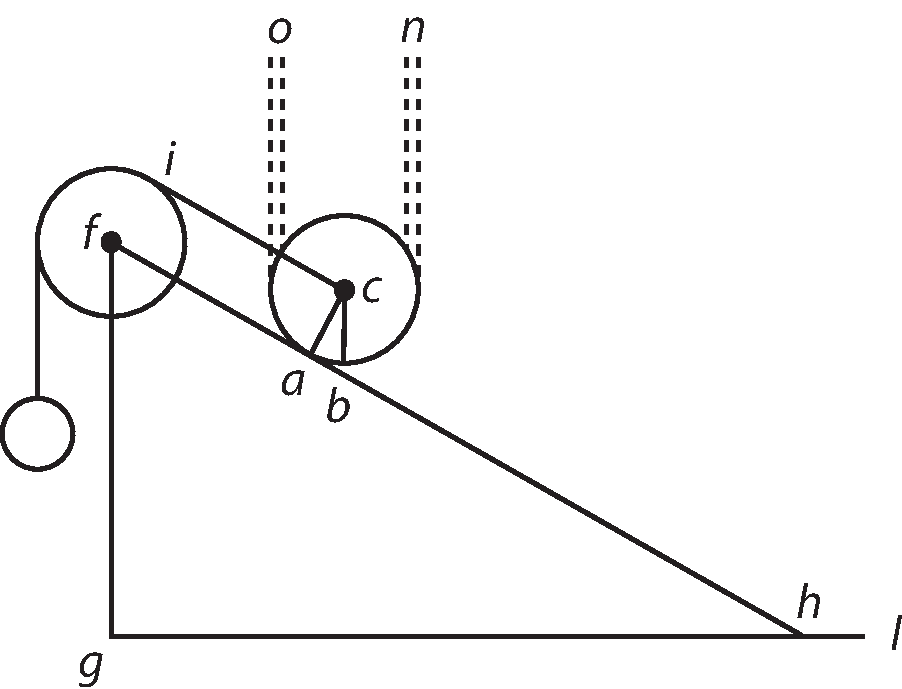
\includegraphics[width=0.47\textwidth]{images/lh0351402127r-1.pdf}\\
 \noindent \centering [\textit{Fig. 1}] 
\end{center}
\pend
\newpage
\pstart \noindent est totum, ratiocinantur de motu eodem \edtext{modo}{\lemma{modo}\Cfootnote{\textsc{I. G. Pardies}, \cite{00296}a.a.O., S. 82f.}} et n. 54 contra id quod ait des Cartes\protect\index{Namensregister}{\textso{Descartes} (Cartesius, des Cartes), Ren\'{e} 1596-1650}, corpus a quiete sua \edtext{sustineri. Si sint maxima duo corpora}{\lemma{sustineri.}\Bfootnote{\textit{(1)} Corpus \textit{(2)} Si corpus \textit{(3)} Si sint maxima duo corpora \textit{L}}} in bilance, \edtext{in aequilibrio, granum sabulis}{\lemma{bilance,}\Bfootnote{\textit{(1)} grani sabulis \textit{(2)} qu \textit{(3)} vince \textit{(4)} adj \textit{(5)} in aequilibrio, granum sabulis \textit{L}}} accedens faciet descendere alterum latus, et levabit oppositum, et quidem si incidat celeritate sua, inprimis (si aer non obstare \edtext{intelligatur).}{\lemma{intelligatur).}\Cfootnote{\textsc{I. G. Pardies}, \cite{00296}a.a.O., S. 88-92.}}
\pend 
\pstart%
\textso{60} Vis sans fin, est celle, \textit{qui engraine dans une roue à}
\edlabel{035,14,02_127r_a1}%
\edtext{}{{\xxref{035,14,02_127r_a1}{035,14,02_127r_a2}}{\lemma{\textit{dents.}}\Bfootnote{\textit{(1)} Le mouuement est tousjours pro \textit{(2)} \textso{61.} \textbar\ \textso{62} \textit{erg.} \textbar\ Quod motus est proportionalis \textit{L}}}}%
\edtext{\textit{dents.}}{\lemma{\textit{dents.}}\Cfootnote{\cite{00296}\textsc{I. G. Pardies}, a.a.O., S. 99.}}
\pend 
\count\Bfootins=1200
\count\Cfootins=1200
\pstart 
%\protect\begin{wrapfigure}{l}{0.3\textwidth}          
%\protect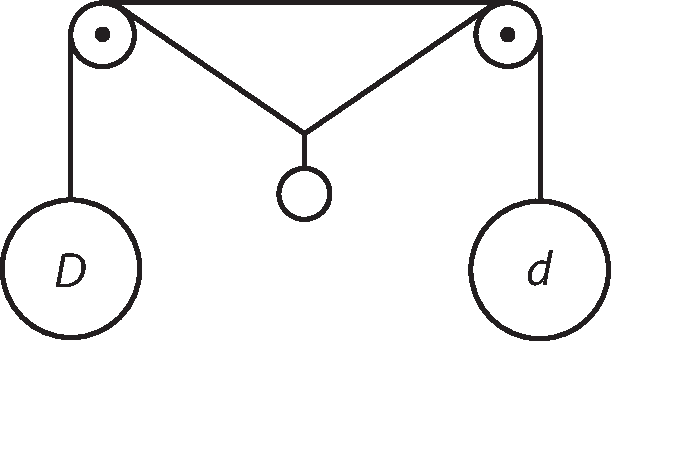
\includegraphics[width=0.3\textwidth]{images/lh0351402127r-2.pdf}
%\caption{Bildbeschreibung}
%\end{wrapfigure}
\textso{61.}
\textso{62}
Quod motus est proportionalis\edlabel{035,14,02_127r_a2} viribus,
%\pstart 
%\textso{60} Vis sans fin, est celle, \textit{qui engraine dans une roue a} \edtext{\textit{dents.}}{\lemma{\textit{dents.}}\Cfootnote{\cite{00296}\textsc{I. G. Pardies}, a.a.O., S. 99.}}
%\pend 
%\count\Bfootins=1200
%\count\Cfootins=1200
%\pstart 
%%\protect\begin{wrapfigure}{l}{0.3\textwidth}          
%%\protect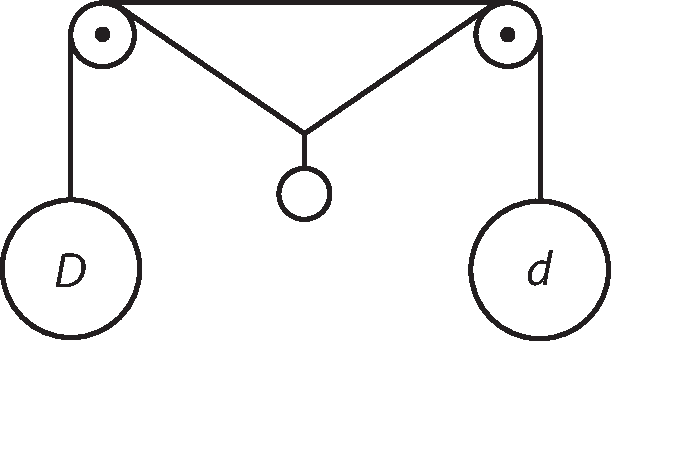
\includegraphics[width=0.3\textwidth]{images/lh0351402127r-2.pdf}
%%\caption{Bildbeschreibung}
%%\end{wrapfigure}
%\textso{61.} \edtext{\textso{62}}{\lemma{}\Bfootnote{\textso{62.} \textit{erg. L}}} \edtext{Quod motus est proportionalis}{\lemma{dents.}\Bfootnote{\textit{(1)} Le mouuement est tousjours pro \textit{(2)} \textso{61.} \textbar\ \textso{62.} \textit{erg.} \textbar\ Quod motus est proportionalis \textit{L}}} viribus, 
et quod majoribus opus non sit viribus ferendo corpori centum librarum in altitudinem pedis, vel \edtext{librae in altitudinem 100 pedum}{\lemma{librae}\Bfootnote{\textit{(1)} 100 librarum \textit{(2)} in altitudinem 100 pedum \textit{L}}}. Sed hoc non satisfacere animo, ut pro principio demonstrationum statui \edtext{queat.}{\lemma{queat.}\Cfootnote{\textsc{I. G. Pardies}, \cite{00296}a.a.O., S. 101f.}} Imo demonstratio quam ex Galilaeo\protect\index{Namensregister}{\textso{Galilei} (Galilaeus, Galileus), Galileo 1564-1642}
attulit non est \edtext{interna, et cogit non ostendit. Ut}{\lemma{interna,}\Bfootnote{\textit{(1)} sed e \textit{(2)} sed a \textit{(3)} et cogit non ostendit. Ut \textit{L}}} \textit{Geometriae Elementorum} Euclidis\protect\index{Namensregister}{\textso{Euklid} (Euclides) von Alexandria 287-212 v. Chr.}
in comparatione Geometriae indivisibilium. 
\pend 
\pstart \edtext{\textso{66-69} Utcunque magna pondera}{\lemma{\textso{66-69}.}\Bfootnote{\textit{(1)} Corpus \textit{(2)} Utcunque magna pondera \textit{L}}} \edtext{$d D$}{\lemma{$d D$}\Bfootnote{\textit{erg. L}}} suspendantur extremis chordae per duas trochleas incedentis, medium tamen pondus quantulumcunque nonnihil ea attrahet, seu chordam \edtext{attollet}{\lemma{attollet}\Cfootnote{\textsc{I. G. Pardies}, \cite{00296}a.a.O., S. 110f.}} ita etsi nullum sit pondus $e$ ipsum pondus chordae pro eo pot\-erit sumi, ideoque impossibile esse chordam qualiscunque viribus perfecte \edtext{tendere.}{\lemma{tendere.}\Cfootnote{\cite{00296}\textsc{I. G. Pardies}, a.a.O., S. 118f.}} Ego demonstrationem istam, esse puto paralogismum.
\pend
%\advanceline{-2}
\vspace*{2.5em}
\pstart
\begin{center}
  %\protect\begin{wrapfigure}{l}{0.3\textwidth}          
\noindent 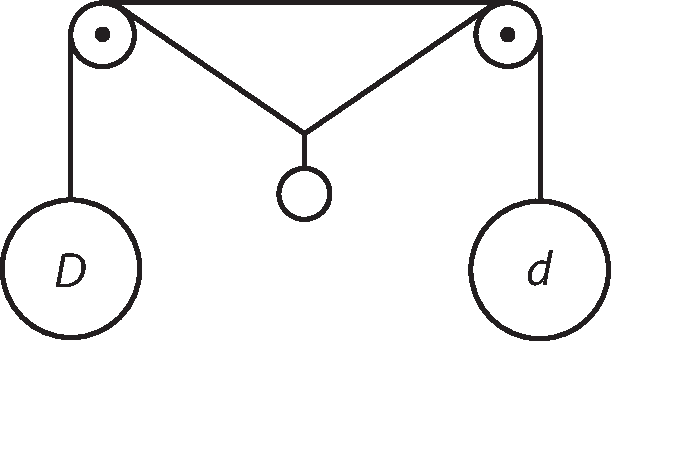
\includegraphics[trim = 0mm 10mm 0mm 0mm, clip, width=0.33\textwidth]{images/lh0351402127r-2.pdf}\\
\noindent \hspace{-8mm}[\textit{Fig. 2}] 
\end{center}
\pend
\count\Bfootins=1500
\count\Cfootins=1500
 


 




\chapter[\scriptsize\uppercase{Pardies, Discours du mouvement local, 1670}]{\uppercase{Anstreichungen und Anmerkungen in Pardies, Discours du mouvement local, 1670}
\newline\lbrack XXX \textendash\ XXX\rbrack}
\addcontentsline{toc}{chapter}{\thechapter\enskip Anstreichungen und Anmerkungen in Pardies, Discours du mouvement local, 1670 \lbrack XXX \textendash\ XXX\rbrack}
\vspace{8mm}
     \begin{ledgroupsized}[r]{120mm}
\footnotesize 
\pstart 
\noindent\textbf{\"{U}berlieferung:}
\pend
\end{ledgroupsized}
\begin{ledgroupsized}[r]{114mm}
\footnotesize 
\pstart \parindent -6mm
\makebox[6mm][l]{\textit{LiH}}%
Anstreichungen und Anmerkungen in \textsc{I.G. Pardies},\cite{00204} \textit{Discours du mouvement local}, Paris 1670: \textsc{Hannover}, GWLB,
 Leibn. Marg. 28. \pend
\end{ledgroupsized}

\vspace*{5mm}
\begin{ledgroup}
\footnotesize 
\pstart
\noindent\footnotesize{\textbf{Datierungsgr\"{u}nde:}
Leibniz verkehrte mit Pardies in Paris (siehe hierzu etwa \textit{LSB} II, 1 N.~133, S.~442; III,~1 N.~9, S.~42) und beschäftigte sich mit dessen mathematischen Werken eingehend während seines Pariser Aufenthaltes,
wie dies u.a. die Stücke \textit{LSB} VII, 3 N.~6, N.~26 und N.~38\textsubscript{12} belegen.
Die vorliegenden Marginalien dürften aber spätestens zu dem Zeitpunkt  verfasst worden sein, als Leibniz Pardies' \title{Statique} exzerpiert hat,
d.h. spätestens im Mai 1673 (siehe die Datierungsgründe in N.~7;
%= LH035_14_02_128v.tex + LH035_14_02_127r.tex = Aus und zu I. G. Pardies, La Statique
in N.~44
%= I. G. Pardies, La Statique = Pardies1673.tex
sind ferner Leibniz' Marginalien in seinem Handexemplar von \textit{La statique} ediert).
Denn wie Leibniz selbst zu Beginn von N.~7 referiert,
%= LH035_14_02_128v.tex + LH035_14_02_127r.tex = Aus und zu I. G. Pardies, La Statique
stellt Pardies seine \textit{Statique} als Fortsetzung des \title{Discours du mouvement local} dar
(siehe \cite{00296}\textsc{I.G. Pardies}, \textit{La statique}, Paris 1673, Préface).
%, S.~aij
Es erweist sich demgemäß als plausibel, die vorliegenden Marginalien auf den Zeitraum vom Frühjahr 1672 bis zum Mai 1673 zu datieren.}
\pend
\end{ledgroup}


\vspace*{8mm}
\pstart 
\normalsize
\noindent [Preface p. 1] PREFACE. / \textit{IE ne pretends pas faire ici l'eloge des Mechaniques} [...]\edtext{}{\lemma{}\Afootnote{\textit{Am oberen Rand rechts}: p. 13 negligit magnitudines corporum.\vspace{1mm}}}
\pend 
\count\Afootins=1200
\pstart  
[p. 29] Cequi est manifeste par les mesmes raisons que j'ai apport\'{e}es pour prouver que le mouvement dure to\^{u}jours. Mais il faut remarquer que lorsqu'vn corps a receu successivement plusieurs determinations differentes; il reste affect\'{e} de \edtext{la derniere}{\lemma{}\Afootnote{\textit{Leibniz unterstreicht}: la derniere, \textit{notiert daneben am Rand}: Error. Componuntur omnes in unum conatum \textit{und streicht schließlich die ganze Randbemerkung.}}}, sans que les precedentes fassent aucune impression sur lui.
\pend 
\pstart  
[p. 32] [...] ainsi le corps demeure affect\'{e} de la derniere determination: or cette derniere determination le portoit vers \textit{g}, c'est \`{a} dire qu'il faut prendre l'inclination qu'a la ligne courbe au point \textit{f}: et cette inclination se mesure par la tangente, comme s\c{c}avent les Geometres; ainsi c'est suivant cette tangente que le corps a\edtext{}{\lemma{}\Afootnote{\textit{Unter dem Text, gestrichen}: paralogismus
}} [p. 33] est\'{e} determin\'{e} pour la derniere fois; et par consequent c'est suivant cette ligne qu'il continu\"{e} de se mouvoir.
\pend 
\count\Afootins=1000
\pstart  
[p. 35] [...] tous ces corps continu\"{e}ront de se mouvoir en cercle, la boule \`{a} l'entour du clou o\`{u} elle est suspendu\"{e}: la rou\"{e} \`{a} l'entour de son essieu o\`{u} elle est attach\'{e}e: et la liqueur \`{a} l'entour du centre du vaisseau o\`{u} elle est renferm\'{e}e. De mesme si 
%HS: öffnende edtext-Klammer für Afn hierher versetzt
\edtext{deux corps estant attachez ensemble, sont \'{e}galement agitez vers des endroits differens; il faut necessairement que ces corps opposez se meuvent circulairement \`{a} l'entour du point qui est au milieu d'eux, et c'est}{\lemma{}\Afootnote{\textit{Leibniz unterstreicht}: si deux [...] d'eux, et c'est\vspace{1mm}}} [p. 36] ainsi qu'vn fuseau ou vne pirou\"{e}tte continu\"{e}nt de se mouvoir circulairement; parceque les parties oppos\'{e}es estant attach\'{e}es et vnies entre elles, et de plus estant meu\"{e}s par les doits, en deux sens differens, l'vne d'vn cost\'{e} l'autre de l'autre; il faut que ce fuseau se meuve \`{a} l'entour de soy mesme. Que si de plus ces parties oppos\'{e}es sont pouss\'{e}es in\'{e}galement, en sorte que l'vne soit port\'{e}e vn peu plus \edtext{v\^{i}te vers vn cost\'{e}: alors ce corps outre son mouvement circulaire \`{a} l'entour de soy-mesme, aura vn autre mouvement qui le portera tout entier sur quelques lignes differentes suivant la diversit\'{e} et la combinaison de ces determinations. Et c'est ainsi qu'vne pirou\"{e}tte d\'{e}crit}{\lemma{}\Afootnote{\textit{Leibniz markiert am Rand}: v\^{i}te vers vn cost\'{e} [...] qu'vne pirou\"{e}tte décrit \textit{und notiert}: \Denarius \hspace{1.8mm}Videtur eligi centrum propius parti victae quia si supponatur immobilis seu fixa ipsa erit centrum. Et tanto est propior immobili, quanto victa magis.}} par son essieu sur la table di[p. 36]verses figures entrelass\'{e}es tandis qu'elle se meut avec vne v\^{i}tesse incroyable \`{a} l'entour de son propre centre.
\pend 
\pstart  
[p. 39] [\textit{Gedruckte Marginalie}:] XVII. Dans la rencontre de deux corps il se fait vne \makebox[1.0\textwidth][s]{percussion, qui est mutuelle et \'{e}galement receu\"{e} dans l'vn et dans l'autre corps.}\\
\noindent [\textit{Haupttext}:] Or quoique bien souvent il n'y ait qu'vn corps qui\edtext{}{\lemma{}\Afootnote{\textit{Am Rand}: \Denarius}} se meuve et qui frappe,\hfill
tandis\hfill que\hfill l'autre\hfill demeure\hfill immobile\hfill et\hfill re\c{c}oit\hfill le\hfill coup;\hfill neanmoins\hfill la\hfill percussion\hfill est
\pend 
\vspace{1em}
\pstart
\centering
 \noindent 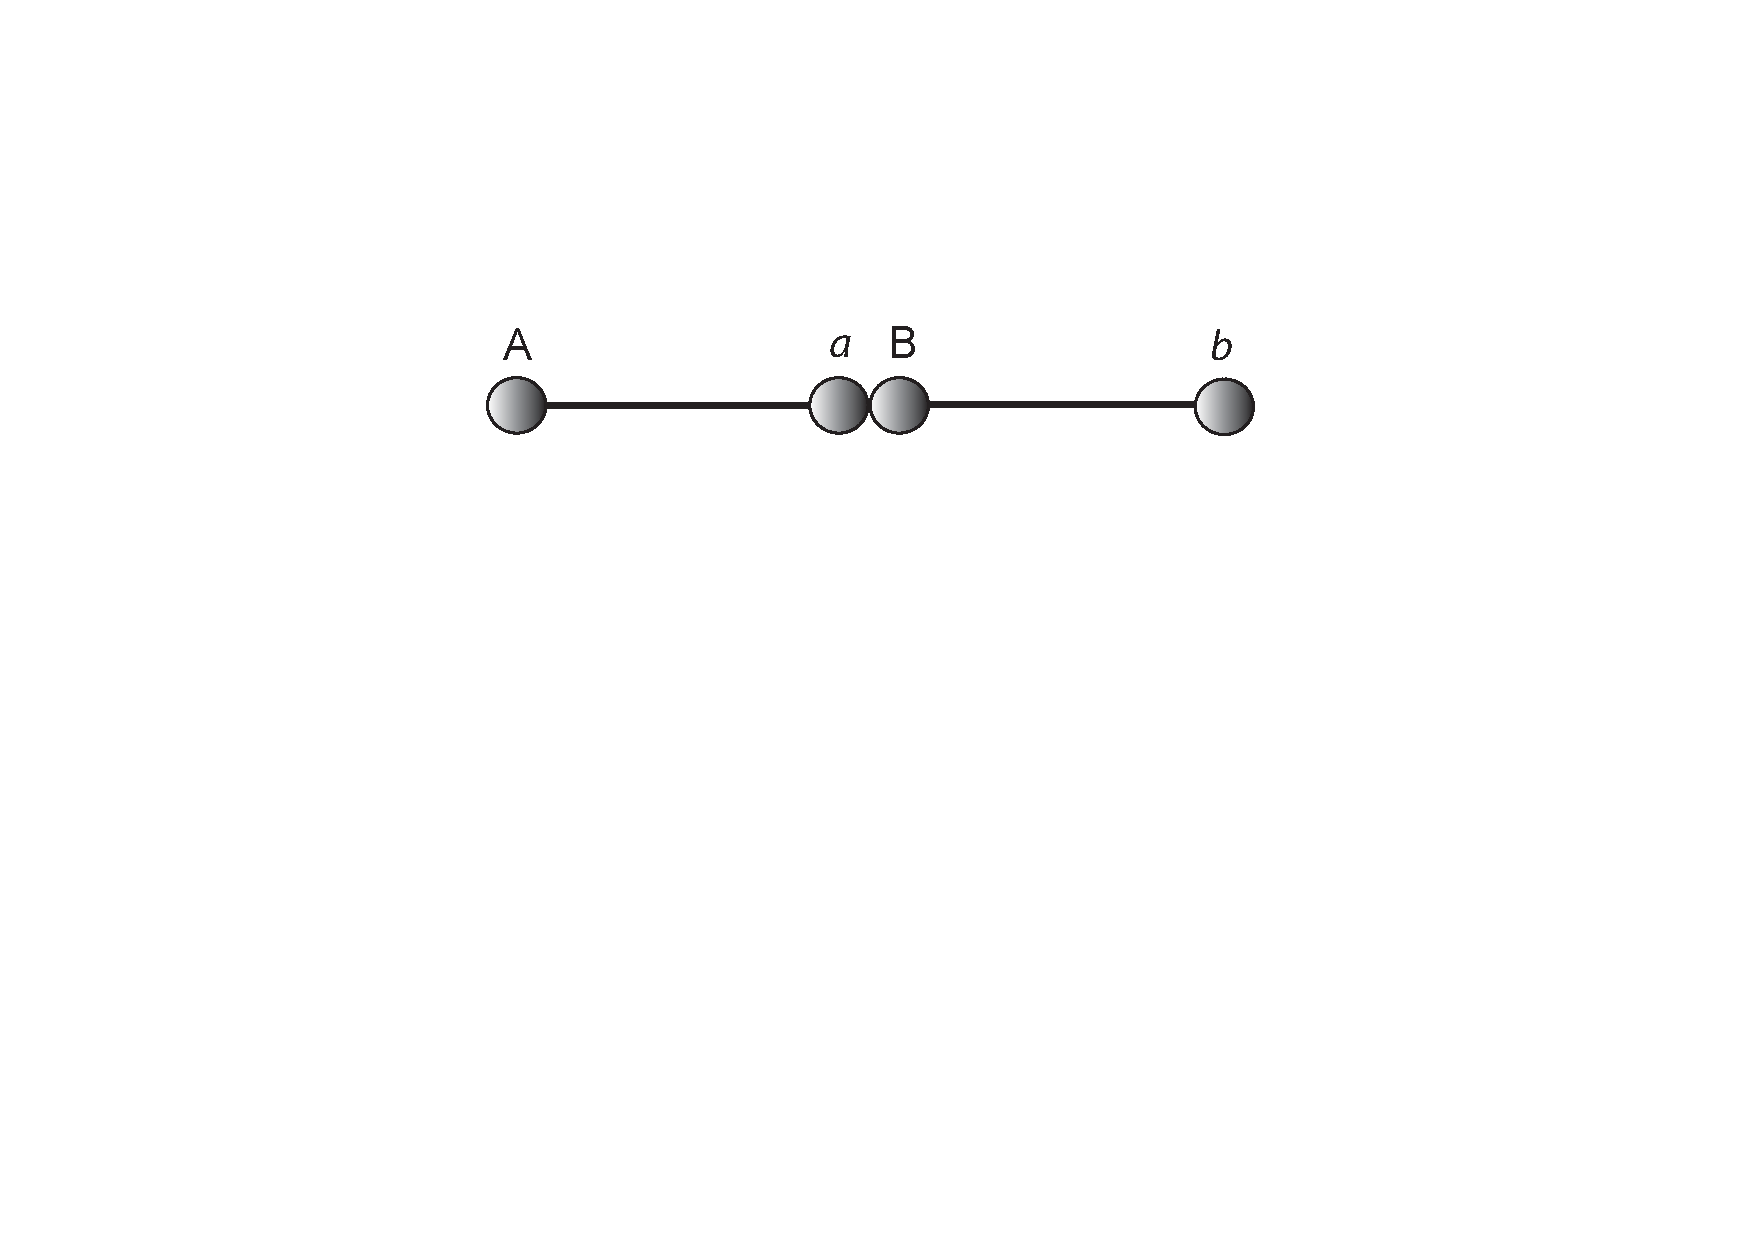
\includegraphics[trim = 0mm -3mm 0mm 0mm, clip, width=0.46\textwidth]{images/pardies1670-d1.pdf}\\
              \noindent \centering [\textit{Fig. 1}] 
\pend
\count\Afootins=1000
\pstart  
\noindent
to\^{u}jours mutuelle et elle est \'{e}galement receu\"{e} dans l'vn et dans l'autre corps: De sorte qu'autant que\edtext{}{\lemma{}\Afootnote{\hspace{1mm}\textit{Unter dem Text}: Il n'y a point de choc ny percussion sans resistance.}} [p. 40] le corps \textit{a} frappe le corps \textit{B}, autant est-il frapp\'{e} luy-mesme. \edtext{Ce que nous concevrons ais\'{e}ment si nous supposons que ces deux corps sont tout-\`{a}-fait semblables en masse, en figure, en}{\lemma{}\Afootnote{\hspace{-1mm}\textit{Leibniz markiert am Rand}: Ce que nous [...] en masse, en figure, en  \textit{und notiert}:
\Denarius}} duret\'{e}, et si de plus nous imaginons qu'ils aient du sentiment, et qu'ils soient capables de ressentir de la douleur quand ils sont frappez: [...]
\pend 
\count\Afootins=1000
\pstart  
[p. 41] Ainsi nous pouvons mettre pour vne maxime generale [p. 42] que \edtext{\textit{lorsque deux corps se frappent, la percussion est mutuelle et \'{e}gale de part et d'autre.}}{\lemma{}\Afootnote{\hspace{0.8mm}\textit{Neben dem kursiv gesetzten Text}: \Denarius}}
\pend 
\pstart  
[p. 42] Puis donc que la percussion que re\c{c}oit le corps \textit{B} est d'vn degr\'{e}, c'est \`{a} dire qu'elle est capable de porter le corps \textit{B} avec vn degr\'{e} de v\^{i}tesse
%HS: öffnende edtext-Klammer für Afn hierher versetzt
\edtext{vers \textit{b}; il faut aussi que la percussion que re\c{c}oit en mesme temps le corps \textit{a} soit aussi d'vn degr\'{e}; c'est \`{a} dire,}{\lemma{}\Afootnote{\hspace{0.8mm}\textit{Leibniz markiert am Rand}: vers \textit{b}; [...] c'est \`{a} dire  \textit{und notiert}:
error\vspace{1.1mm}}} qu'[p. 43]elle puisse porter le corps \textit{a} avec vn degr\'{e} de v\^{i}tesse vers les parties oppos\'{e}es, c'est \`{a} s\c{c}avoir vers \textit{A}.
\pend 
\vspace{1em}
\pstart
\centering
 \noindent 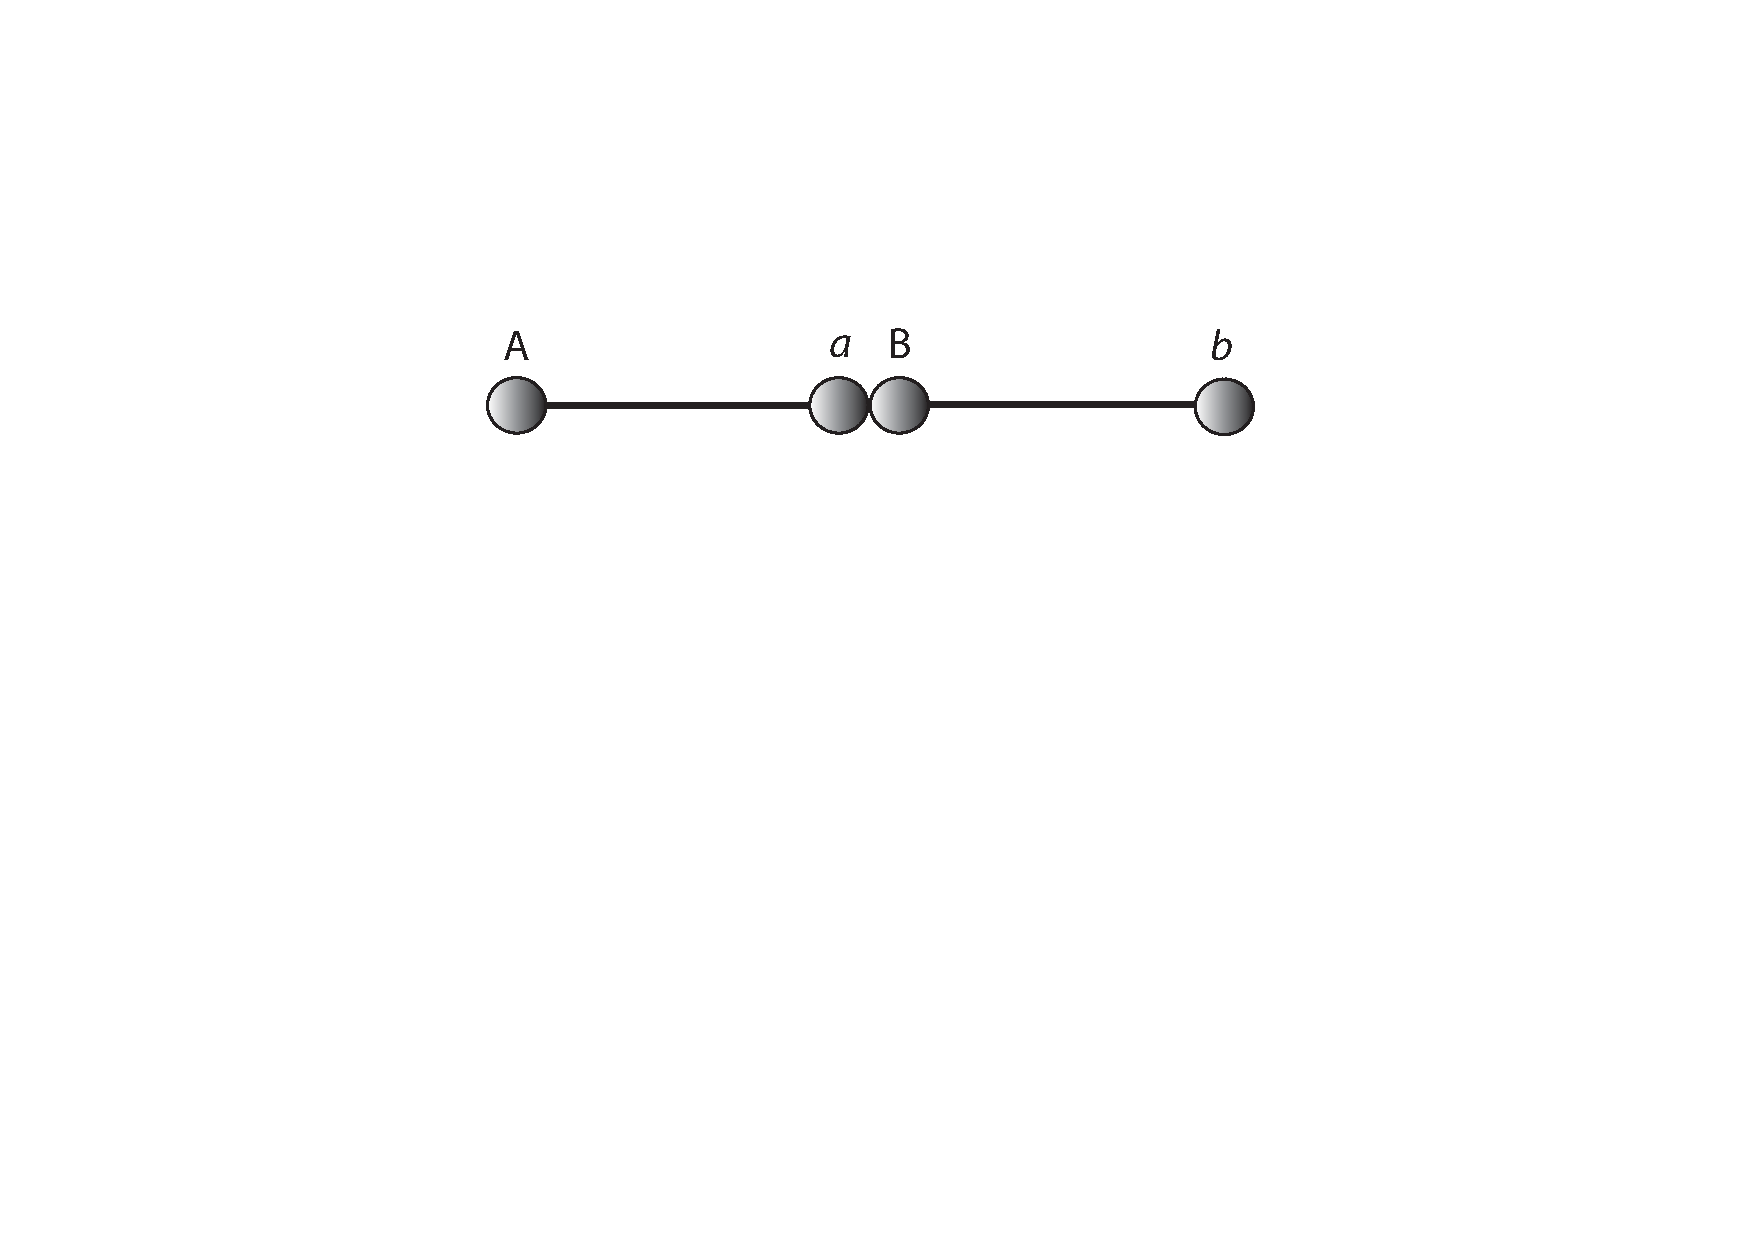
\includegraphics[trim = 0mm -3mm 0mm -5mm, clip, width=0.46\textwidth]{images/pardies1670-d2.pdf}\\
              \noindent \centering [\textit{Fig. 2}] 
\pend
\vspace{1em}
\pstart  
[p. 43] \setline{13}\edtext{Ainsi dans cette percussion le corps \textit{a} donne son mouvement et sa v\^{i}tesse au corps \textit{B}, et demeure cependant luy-mesme immobile.}{\lemma{}\Afootnote{\hspace{-1mm}\textit{Am Rand auf eingeklebtem Zettel}: Alia longe hujus rei ratio quaerenda, a natura pleni seu medii.\vspace{1mm}}}
\pend 
%\newpage
\count\Afootins=1200
\pstart  
[p. 46] D'o\`{u} l'on void encore que la percussion sera d'autant plus grande que cette approche mutuelle se sera plus viste. \edtext{De sorte que \textit{les percussions sont to\^{u}jours comme les v\^{i}tesses respectives}, pourveu que tout le reste soit pareil. Ainsi les deux corps s'approchant chacun}{\lemma{}\Afootnote{\textit{Am Rand auf eingeklebtem Zettel}: La veritable raison en est, parce qu'on peut dire, que
l'un est aussi bien meu vers l'autre, que l'autre vers luy.}} avec vn degr\'{e} de v\^{i}tesse absolu\"{e}, et faisant chacun vn pied de sa part dans vne minute; [...]
\pend 
\count\Afootins=1200
\pstart  
[p. 48] Estant donc certain que la percussion qui se fait en cette rencontre est de deux degrez; [\textit{Auf dieser H\"{o}he gedruckte Marginalie}:] XXI. \textit{Deux corps se mouvant l'vn vers l'autre rebroussent en faisant vn} \edtext{\textit{\'{e}change}}{\lemma{}\Afootnote{\hspace{1.8mm}\textit{Leibniz unterstreicht}: \'{e}change\textit{ und schreibt unter der gedruckten Marginalie}: \Denarius}} \textit{de leur vitesse}. [...]
\pend 
\pstart  
[p. 49] [...] d'vne de deux degrez vers \textit{A} qu'il re\c{c}oit dans la percussion, et d'vne autre d'vn degr\'{e} vers \textit{b}, qu'il avoit auparavant\edtext{}{\lemma{}\Afootnote{\hspace{1.8mm}\textit{Leibniz unterstreicht}: vers \textit{b}, qu'il avoit auparavant \textit{und notiert am Rand}: \Denarius}}; ainsi il luy reste seulement vn degr\'{e} libre d'impression et de v\^{i}tesse qui le porte vers \textit{A}. Et demesme \textit{B} sera port\'{e} vers \textit{b} avec vn degr\'{e} aussi de v\^{i}tesse; de fa\c{c}on que tous deux rebroussent sur la mesme ligne avec la mesme v\^{i}tesse qu'ils \edtext{sont venus}{\lemma{}\Afootnote{\hspace{1.8mm}\textit{Leibniz unterstreicht}: sont venus \textit{und notiert am Rand}: \Denarius}}. Que si nous supposons que l'vn s'avance plus v\^{i}te que l'autre; [...]
\pend 
\count\Afootins=1000
\pstart  
[p. 50] Que si les deux corps se meu[p. 51]vent
vers les mesmes endroits sur vne ligne droite, en sorte que le plus lent allant devant soit enfin \edtext{attrapp\'{e} par le plus v\^{i}te qui le suit}{\lemma{}\Afootnote{\hspace{-0.8mm}\textit{Leibniz unterstreicht}: attrapp\'{e} par le plus v\^{i}te qui le suit}}; alors tous les deux continueront de se mouvoir sur la mesme ligne vers les mesmes endroits; mais ils feront vn \'{e}change de leurs v\^{i}tesses\edtext{}{\lemma{}\Afootnote{\textit{Leibniz unterstreicht}: mais ils feront vn \'{e}change de leurs v\^{i}tesses.\vspace{1mm}}}. Soit le corps \textit{A} meu avec deux degrez de v\^{i}tesse \textit{b}, faisant dans vne minute deux pieds jusques en \textit{a}.
\pend 
\vspace{1em}
\begin{center}
 \noindent 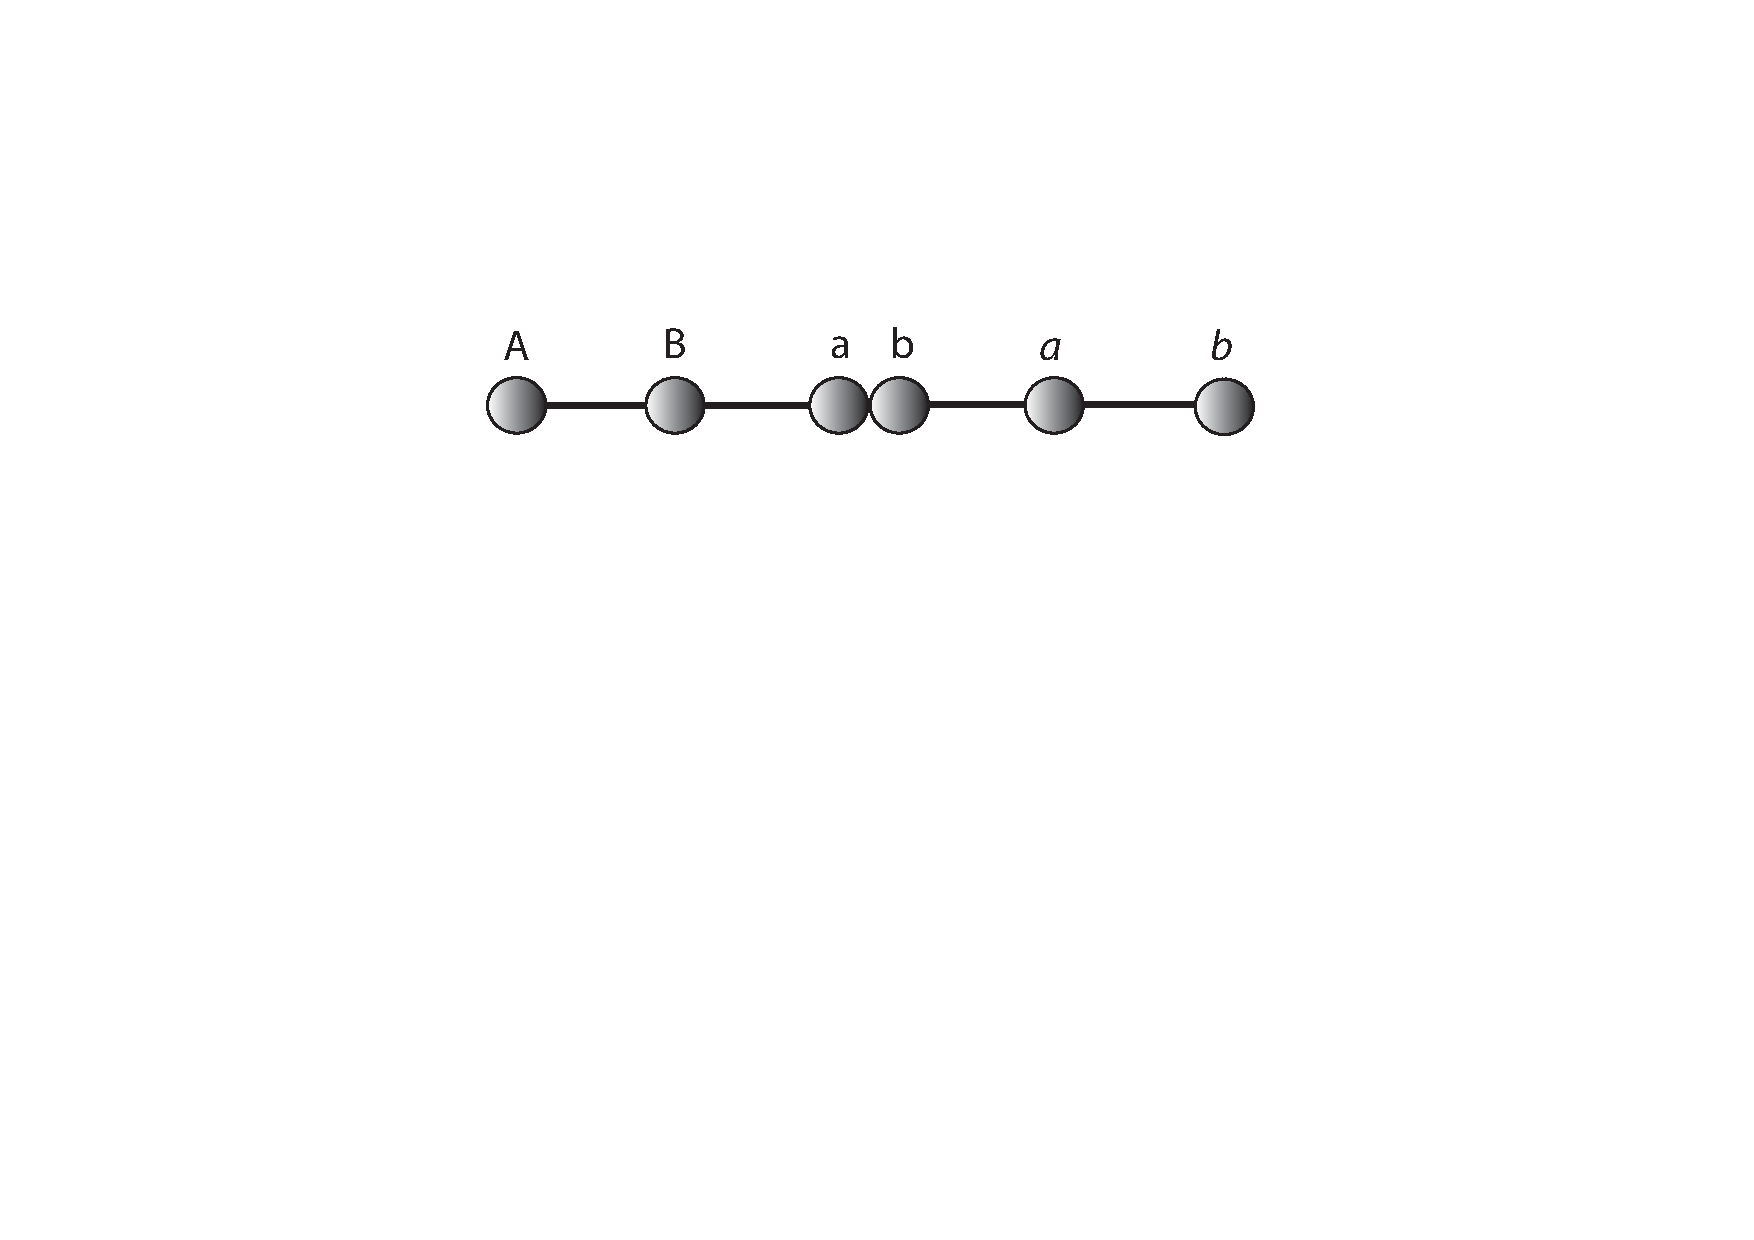
\includegraphics[trim = 0mm -3mm 0mm 0mm, clip, width=0.46\textwidth]{images/pardies1670-d3.pdf}\\
              \noindent \centering [\textit{Fig. 3}] 
\end{center}
\pstart  
[p. 53] \setline{15}Que si le corps qui est frapp\'{e} est tout-\`{a}-fait in\'{e}branlable; il faut voir quelle force aura la percussion, et ce que deviendra le corps qui frappe. [\textit{In dieser H\"{o}he gedruckte Marginalie}:] XXIII. \textit{Vn corps dur venant \`{a} frapper sur vn autre corps in\'{e}branlable, se refl\'{e}chit avec} \edtext{\textit{tout son mouvement.}}{\lemma{}\Afootnote{\textit{Leibniz unterstreicht}: tout son mouvement \textit{und schreibt unter der gedruckten Marginalie}: Il faut chercher d'autres raisons.}}
%diese Bfootnote erscheint nicht im Pdf, ich habe sie aus der Afootnote herausgenommen, verweist sie auf die richtige Stelle????
%{\lemma{chercher}\Bfootnote{\textit{(1)}\ des autres \textit{(2)}\ d'autres \textit{L}}} 
%HS: nachfolgende Bfn bleibt unterdrückt
%\edtext{}{\lemma{chercher}\Bfootnote{\textit{(1)}\ des autres \textit{(2)}\ d'autres \textit{L}}}
\pend
\count\Bfootins=1500
\pstart  
[p. 54] Mais si nous supposons qu'en mesme temps qu'\textit{A} vient frapper la lame en \textit{a}; en mesme temps aussi \textit{B} la vient frapper en \textit{b}; cette lame demeurera immobile, puisqu'elle est frapp\'{e}e \'{e}galement des deux costez opposez; et chaque corps rebroussera avec son degr\'{e} de v\^{i}tesse avec lequel il estoit venu. Car, comme j'ay dit, \edtext{ces deux corps se frappent nonobstant cette lame, comme s'il n'y avoit rien entre-deux}{\lemma{}\Afootnote{\textit{Leibniz unterstreicht}: ces deux [...] rien entre-deux\vspace{1mm}}}; or s'il n'y avoit rien entre-deux, ils rebrousseroient avec leur mesme degr\'{e} [p. 55] de v\^{i}tesse, comme il a est\'{e} prouv\'{e} au \S. 21. ainsi quoique cette lame se trouve l\`{a}; ils ne laisseront pas de rebrousser.
\pend 
\count\Afootins=1200
\pstart  
[p. 56] Et voil\`{a} comment on demonstre qu'vn corps dur venant \`{a} frapper vn autre corps dur inflexible et in\'{e}branlable, se refl\'{e}chit \edtext{avec tout son mouvement: ce que je ne pense pas que personne ait encore demonstr\'{e}.}{\lemma{}\Afootnote{\textit{Leibniz unterstreicht}: avec tout [...] encore demonstr\'{e} \textit{und notiert am Rand}: personne ait encore demonstr\'{e}.}}
\pend 
\pstart  
[p. 66] [...] parce-qu'alors la percussion seroit plus \edtext{droite: et en effet si l'on veut en faire le calcul (ce qui est fort ais\'{e} \`{a} faire sur celuy mesme qu'a fait c\'{e}t Auteur\protect\index{Namensregister}{\textso  {},}) on trouvera que l'obliquit\'{e} de ces mouvemens est to\^{u}jours toute telle qu'il faut pour faire la diversit\'{e} que nous voions dans les percussions d'vn corps qui tombe.}{\lemma{}\Afootnote{\textit{Leibniz markiert am Rand}: droite: et en effet [...] d'vn corps qui tombe.}}
\pend 
\pstart  
L'AUTRE remarque est sur ce que j'ay ve\^{u} dans quelques-vnes de nos citadelles, o\`{u} ceux qui les ont basties, \edtext{ont prefer\'{e} l'agr\'{e}emt des yeux \`{a} la force des}{\lemma{}\Afootnote{\hspace{-0.8mm}\textit{Leibniz unterstreicht}: ont prefer\'{e} l'agr\'{e}emt des yeux \`{a} la force des\vspace{1mm}}} murailles, lorsqu'au lieu de les faire tout-vnies, ils les ont diversifi\'{e}es de beaucoup d'ornemens de pierres qui avancent au dessus des autres: [...]
\pend 
%\newpage
\pstart  
[p. 67] Je dis que si toute cette variet\'{e} est agreable \`{a} la veu\"{e}; elle est aussi tres-desavantageuse pour la d\'{e}fense. \edtext{Car ces enfonceures et ces saillies de pierres donnent aux batteries obliques du canon le mesme avantage et la mesme force qu'ont les batteries droites. De-sorte que le boulet, qui}{\lemma{}\Afootnote{\hspace{-0.8mm}\textit{Leibniz markiert am Rand}: Car ces enfonceures [...] le boulet, qui \textit{und unterstreicht}: Car ces enfonceures [...] et la mesme}} venant de biais ne feroit qu'effleurer le mur s'il l'avoit trouv\'{e} tout plat; [...]
\pend 
\count\Afootins=1000
%\newpage
\pstart  
[p. 70] IL faut remarquer \edtext{qu'il n'est pas vrai qu'il y ait to\^{u}jours autant de mouvement absolu apr\'{e}s la percussion, qu'il y en a[p. 71]voit}{\lemma{}\Afootnote{\textit{Leibniz unterstreicht}: qu'il n'est pas vrai [...] qu'il y en avoit}} devant. Mais il est fort ais\'{e} \`{a} demonstrer \edtext{que le mouvement respectif est to\^{u}jours le mesme}{\lemma{}\Afootnote{\textit{Leibniz unterstreicht}: que le mouvement respectif est to\^{u}jours le mesme}}; en-sorte que les corps s'\'{e}loignent mutuellement l'vn de l'autre apr\'{e}s la percussion, aussi v\^{i}te qu'ils s'en approchoint devant.
\pend 
\pstart  
[p. 71] Et mesme apr\'{e}s que j'aurai expliqu\'{e} les mouvemens qui se font dans le plein; je croy qu'il me seroit facile, de prouver qu'ayant \'{e}gard generalement \`{a} tous les corps qui sont dans tout l'vnivers, \edtext{il y a presentement autant}{\lemma{}\Afootnote{\textit{Leibniz unterstreicht}: il y a presentement autant}} \edtext{de mouvement respectif, ni plus ni moins, qu'il y en avoit au commencement de la creation du monde}{\lemma{}\Afootnote{\hspace{-0.8mm}\textit{Leibniz markiert am Rand}: de mouvement respectif, [...] creation du monde.\vspace{1mm}}}.
\pend 
\count\Afootins=1000
\pstart  
[p. 72] Il est encore \`{a} remarquer que \edtext{le point du milieu}{\lemma{}\Afootnote{\textit{Leibniz unterstreicht}: le point du milieu \textit{und notiert hierzu}: Hugenii\protect\index{Namensregister}{\textso{Huygens}, Christiaan (1629-1695)} centrum gravitatis}} d'entre les deux corps se meut to\^{u}jours vniformement sur vne ligne droite, tirant sans aucune interruption vers les mesmes endroits.
\pend 
\count\Afootins=1000
\pstart  
[p. 72] On s'estonnera sans doute que dans toutes les regles precedentes je n'aye point fait mention de l'\'{e}galit\'{e} ou de l'in\'{e}galit\'{e} des corps qui se frappent. [p. 73] Et il semble d'abord qu'afin que ce que je viens de dire soit veritable it faut que je suppose que le corps sont parfaitement \'{e}gaux: [...] [\textit{Daneben gedruckte Marginalie:} p. 72] XXXI. \textit{Tout ces regles sont veritables, soit que les corps soient} [p. 73] \edtext{\textit{\'{e}geaux; soit qu'ils ne le soient pas.}}{\lemma{}\Afootnote{\textit{Leibniz markiert am Rand}: \textit{\'{e}gaux; soit qu'ils ne le soient pas.}}}
\pend 
\count\Afootins=1000
\pstart  
[p. 74] \edtext{Et si l'on y prend garde la force de la raison que j'ai apport\'{e}e au \S. 16. est to\^{u}jours la mesme}{\lemma{}\Afootnote{\textit{Am Rand und zwischen den Zeilen}: Error.\vspace{1mm}}} quoique les corps soient de differentes grandeurs. Car le corps frapp\'{e} estant tout-\`{a}-fait indifferent \`{a} demeurer en repos ou \`{a} prendre le mouvement, et tout l'effect de la percussion venant de l'impenetrabilit\'{e} des corps:
%diese Bfootnote erscheint nicht im Pdf, ich habe sie aus der Afootnote herausgenommen, verweist sie auf die richtige Stelle????
%HS: Bfn bleibt in dieser Form unterdrückt.
%\edtext{}{\lemma{Supponuntur d'autres}\Bfootnote{\textit{(1)}\ force \textit{(2)}\ vitesse \textit{L}}}
%HS: Bfn bezieht sich auf Afn/Marginalie und wird als Marginalienapparat wie folgt wiedergegeben (am besten am Ende der Seite, da aber die Umbrüche nicht feststehen vorerst direkt bei der entsprechenden Afn):
\edtext{}{\lemma{}\Afootnote{\hspace{0.8mm}\textit{Am Rand auf \"{u}berstehender Papierlasche}: Sans le mouuement dans un liquide il n'y auroit point de difference entre la\textsuperscript{[a]} vitesse absolue et respective, et par consequent ces regles precedentes ne reussiront pas.
\vspace{2mm}
\\
%Hier Marginalienapparat mit dem (korrigierten) Text der Bfn:
\footnotesize
\textsuperscript{[a]} la\ \textit{(1)}\  force \textit{(2)}\ vitesse \textit{L}\vspace{1mm}}} 
%HS: Bfn bleibt in dieser Form unterdrückt.
%\edtext{}{\lemma{Supponuntur d'autres}\Bfootnote{\textit{(1)}\ force \textit{(2)}\ vitesse \textit{L}}}
si nous supposons que le corps frapp\'{e} soit plus grand, pourveu que toutes ses parties soient bien vnies ensemble, il faudra qu'il se meuve de la mesme v\^{i}tesse que se meut le corps qui frappe, [...]
\pend 
\count\Afootins=1200
\pstart 
[p. 76] Si cette substance est parfaitement fluide, c'est-\`{a}-dire si toutes ses parties, aussi bien les petites que les grandes, sont flexibles et liquides: [...] [\textit{Daneben gedruckte Marginalie}:] XXXII. \textit{Vn corps se meut dans le plein, aussi librement que dans le vuide.}\edtext{}{\lemma{}\Afootnote{\textit{Leibniz markiert am Rand die gesamte gedruckte Marginalie.\vspace{1mm}}}}
\pend 
\pstart  
[p. 77] [...] mais ces parties de la liqueur estant pouss\'{e}es, en poussent d'autres; et ainsi \edtext{jusqu'\`{a} l'extremit\'{e}}{\lemma{}\Afootnote{\textit{Leibniz unterstreicht}: jusqu'\`{a} l'extremit\'{e}, \textit{und notiert am Rand}: Hoc nihil est. Exiguum circulum faciunt tantum.\vspace{1mm}}}, d'o\`{u} il se fait vne reflexion par laquelle les parties qui se trouvent apr\'{e}s le corps dur, sont pouss\'{e}es avec la mesme force pour suivre ce mesme corps.
\pend 
\pstart  
[p. 78] [...] il n'est pas possible que les parties qui devancent le corps se meuvent sans que les parties qui suivent le mesme corps ne se meuvent aussi avec la mesme force. Ainsi autant que le corps dur \edtext{est retard\'{e}}{\lemma{}\Afootnote{\textit{Leibniz unterstreicht}: est retard\'{e} \textit{und notiert am Rand}: Pourquoy dans l'hypothese de l'auteur ils ne doivent point retarder, puisque la grandeur ny fait rien.\vspace{-0.5mm}}} par les parties qui le precedent, autant est-il repouss\'{e} par celles qui le suivent, et par consequent si le mouvement a vne fois commenc\'{e}, il doit continuer comme si c'estoit dans le vuide.
\pend 
\pstart  
[p. 79] [...] la communication de l'impression ne se peut faire parfaitement, et ainsi les parties posterieures de la liqueur ne seront pas tant pouss\'{e}es que les anterieures, et par consequent ne pousseront pas tant le corps dur, que celles de devant \edtext{le retardent}{\lemma{}\Afootnote{\hspace{-1.8mm}\textit{Leibniz unterstreicht}: le retardent.\vspace{1mm}}}. Et c'est pour cette raison que tous nos mouvements cessent [...]
%\edtext{}{\lemma{entre la}\Bfootnote{\textit{(1)} force \textit{ (2) } vitesse \textit{L}}}
\pend 
%\newpage
\count\Afootins=1200
\pstart  
[p. 82\,f.] [\textit{gedruckte Marginalie}:] XXXV. \edtext{\textit{Lorsque les corps sont in\'{e}gaux, les percussions se font dans le plein autrement que dans le vuide}}{\lemma{}\Afootnote{\textit{Leibniz markiert am Rand die gedruckte Marginalie und notiert darunter}: Je doute fort que le plein en repos differe du vuide.}}. [\textit{Haupttext}:] Mais si le corps frappant est plus grand, il faut necessairement qu'il ne re\c{c}oive pas tant d'effet de la percussion que l'autre, parcequ'il est emport\'{e} avec plus de violence par la liqueur qui l'environne; car nous voions qu'vne poutre emport\'{e}e par le [p. 83] courant d'vne riviere a bien plus d'effet quand elle vient \`{a} heurter contre vn pont ou contre vn moulin, que n'auroit\hfill pas\hfill vn\hfill b\^{a}ton\hfill emport\'{e}\hfill aussi\hfill par\hfill la\hfill mesme\hfill riviere;\hfill quoique\hfill d'ailleurs\hfill la\hfill poutre
\pend
\newpage
\pstart \noindent n'allast pas plus v\^{i}te que le b\^{a}ton: \edtext{et cela parce que la poutre venant \`{a} heurter est encore pouss\'{e}e par la grande quantit\'{e} d'eau qui l'environne, au-lieu que le b\^{a}ton l'est fort peu \`{a} cause du peu de place qu'il occupe et du peu d'eau dont il est emport\'{e}. Ainsi donc si le petit corps est en repos et que le grand vienne \`{a} le}{\lemma{}\Afootnote{\textit{Am Rand}: Si la poutre n'avoit qu'une petite base de la grandeur d'un baston, qui la so\^{u}tiendroit dans l'eau le m\^{e}me arriveroit. Ce n'est donc pas la grandeur de l'eau qui le pousse mais sa propre.}} frapper; [...]
\pend 
\pstart  
[p. 84] Au-contraire si le grand est en repos, le plus petit apr\'{e}s avoir frapp\'{e} l'autre et luy avoir communiqu\'{e} vne partie de son mouvement, se refl\'{e}chira en perdant vne partie de sa v\^{i}tesse. Et de tout ceci il paroist \edtext{qu'Aristote n'est pas si blasmable}{\lemma{}\Afootnote{\textit{Leibniz unterstreicht}: qu'Aristote n'est pas si blasmable}} que quelques-vns pretendent, lorsque pour expliquer les causes de la continuation des mouvemens que nous voions, il a emploi\'{e} le \textit{medium}, c'est-\`{a}-dire la substance liquide dans laquelle nos corps se meuvent.
\pend 
\count\Afootins=1200
\count\Cfootins=1200
\pstart  
[p. 85] [...] de la facilit\'{e} qu'ils ont de se condenser ou de se rarefier, et de beaucoup d'autres choses qui ne peuvent nous estre connu\"{e}s non plus qu'vne infinit\'{e} d'autres empeschemens dont les combinaisons peuvent diversifier infiniment tous les effets des percussions. Seulement je \edtext{puis dire qu'en faisant vne certaine hypothese, qui paroist assez naturelle, on peut faire voir par les regles precedentes, que les percussions des corps in\'{e}gaux se feront de la maniere que veut Monsieur Hugens\protect\index{Namensregister}{\textso {Huygens}, Christiaan (1629-1695)} dans le dernier \textit{\edtext{Journal des S\c{c}avans.}{\lemma{Journal des S\c{c}avans}\Cfootnote{\cite{01118}\textsc{C. Huygens}, \glqq Extrait d'une lettre à l'auteur du Journal\grqq, \title{JS}, 18.~März 1669, S.~22-24 (\cite{00113}\title{HO} VI, S.~383-386).}}} Mais je ne veux pas m'ar}{\lemma{}\Afootnote{\textit{Leibniz markiert am Rand}: puis dire qu'en [...] je ne veux pas}}[p. 86]\edtext{rester l\`{a} davantage, peut-estre trouverai-je en quelque autre}{\lemma{}\Afootnote{\textit{Am Rand}: pourquoy non icy.}} rencontre occasion d'en parler plus amplement.
\pend 
\count\Cfootins=1500
%\newpage
\pstart  
[p. 87] Je ne veux pas marquer les mesures de ces refractions, parce que cela a est\'{e} fait par d'autres, et que leurs demonstrations se peuvent fort bien accommoder avec les choses que j'ai ici avanc\'{e}es. Je ne parle pas non plus ici de la refraction de \edtext{la lumiere}{\lemma{}\Afootnote{\textit{Leibniz unterstreicht}: la lumiere}}, parce que je croi qu'elle se fait tout autrement, \edtext{c'est-\`{a}-dire par des causes et des moiens tout differens}{\lemma{}\Afootnote{\textit{Leibniz unterstreicht}: c'est-\`{a}-dire par des causes et des moiens tout differens}}, comme je pourrois faire voir si je faisois quelques [p. 88] autres discours du mouvement.
\pend 
%\newpage
\pstart  
[p. 88] Il faudroit encore parler du mouvement des liqueurs, tant de leur chute que de leur faillie, comme aussi de leurs ondulations et de choses semblables: mais tout cela merite autant de discours particuliers. Et \edtext{comme je croy avoir trouv\'{e} quelque chose de nouveau sur ces matieres, je ne feray point}{\lemma{}\Afootnote{\textit{Leibniz markiert am Rand}: comme je croy [...] je ne feray point}} difficult\'{e}, de donner au public mes pens\'{e}es \`{a} examiner, si je voi que ce premier dis[p. 89]cours n'ait pas est\'{e} jug\'{e} tout-\`{a}-fait indigne d'estre le\^{u} par les personnes qui se plaisent \`{a} de semblables matieres.
\pend 
\count\Afootins=1200
%\newpage
\pstart  
[p. 98] \textit{Ie vous dis dernierement lorsque nous estions ensemble, non pas \`{a} la verit\'{e} que la lumiere se mouvoit en vn instant, comme vous m'\'{e}crivez; mais (ce que vous croyez estre la mesme chose) que du corps lumineux elle parvenoit en vn instant jusqu'\`{a} nos yeux: et mesme j'ajo\^{u}tai que je pensois s\c{c}avoir cela si certainement,} \edtext{\textit{que si on me pouvoit convaincre de fausset\'{e} l\`{a}-dessus, j'estois tout prest d'avouer que je ne s\c{c}avois rien du tout en Philosophie. Et vous au contraire, vous assuriez que la}}{\lemma{}\Afootnote{\textit{Leibniz markiert am Rand}: \textit{si on me pouvoit} [...] \textit{vous assuriez que la}}} \textit{lumiere ne se mouvoit pas en vn instant; et vous disiez avoir trouv\'{e} vn moyen d'en faire l'experience, par lequel il seroit ais\'{e} devoir} [p. 99] \textit{qui de nous deux se trompoit en cela.}
\pend 
\pstart 
[p. 99] \edtext{\textit{Si quelqu'vn portant de nuit vn flambeau \`{a} la main, et le faisant mouvoir, jette la veu\"{e} sur vn miroir \'{e}loign\'{e} de luy d'vn quart de lieu\"{e}, il pourra tres-ais\'{e}ment remarquer, s'il sentira le mouvement qui se fait en sa main, auparavant que de le voir par le moyen du miroir.}}{\lemma{}\Afootnote{\textit{Leibniz markiert am Rand}: Si quelqu'vn [...] le moyen du miroir.}} \textit{Et vous vous assuriez tellement sur cette experience, que vous estiez prest de croire que toute vostre Philosophie estoit fausse,} [...]
\pend 
\count\Afootins=1200
%\newpage
\pstart  
[p. 118] Ainsi la lumiere qui est maintenant parvenu\"{e} \`{a} nous, estant sortie de C, o\`{u} estoit la Lune demi-heure auparavant, nous doit faire voir la Lune en \edtext{E}{\lemma{}\Afootnote{\textit{Leibniz ersetzt} E \textit{durch} C.}}, en quelque part du monde qu'elle se puisse maintenant trouver, quand elle seroit demeur\'{e}e immobile, ou qu'elle auroit est\'{e} transport\'{e}e: [...]
\pend 
\pstart  [p. 146] M. Descartes se sert tres-mal du principe qui a est\'{e} expliqu\'{e} 
\edtext{au \S. 13.}{\lemma{au \S. 13.}\Cfootnote{\textsc{I. G. Pardies},\cite{00204} \textit{Discours du mouvement local}, Paris, 1670, S. 33.}} 
\edtext{\textit{Que tout corps qui se meut autour d'vn centre, fait effort pour s'en \'{e}loigner.} On peut faire voir qu'il s'est tromp\'{e} en}{\lemma{}\Afootnote{\hspace{-1.3mm}\textit{Leibniz markiert am Rand}: \textit{Que tout corps} [...] s'est tromp\'{e} en\vspace{1mm}}} [p. 147] voulant expliquer par l\`{a} la pesanteur des corps. Aussi ne pretend-on pas donner \`{a} ce principe toute l'\'{e}tendu\"{e} que luy donne M. Descartes.
\pend 
\pstart  [p. 147] L'auteur de ce discours est pleinement persuad\'{e}, que quand bien il n'y auroit point de saintes Ecritures, l'hypothe[p. 148]\edtext{se qui met la terre immobile, est preferable \`{a} toute autre.}{\lemma{}\Afootnote{\textit{Leibniz unterstreicht und markiert am Rand}: qui met la terre immobile, est preferable \`{a} toute autre.}} On a seulement voulu faire voir que c\'{e}t argument n'est pas convainquant: il y en a d'autres qui sont meilleurs, sur tout celuy qui a est\'{e} fait valoir en de fort belles occasions; pris du mouvement \edtext{tonique}{\lemma{}\Afootnote{\textit{Leibniz unterstreicht}: tonique}} de l'aiman.
\pend
 \count\Afootins=1500
 \count\Bfootins=1500
 \count\Cfootins=1500



\chapter[\scriptsize\uppercase{Pardies, La Statique, 1673}]{\uppercase{Anstreichungen und Anmerkungen in Pardies, La Statique, 1673}
\newline\lbrack XXX \textendash\ XXX\rbrack}
\addcontentsline{toc}{chapter}{\thechapter\enskip Anstreichungen und Anmerkungen in Pardies, La Statique, 1673 \lbrack XXX \textendash\ XXX\rbrack}
\vspace{8mm}
     \begin{ledgroupsized}[r]{120mm}
\footnotesize 
\pstart 
\noindent\textbf{\"{U}berlieferung:}
\pend
\end{ledgroupsized}

\begin{ledgroupsized}[r]{114mm}
\footnotesize 
\pstart \parindent -6mm
\makebox[6mm][l]{\textit{LiH}}%
Anstreichungen und Anmerkungen in \textsc{I. G. Pardies}, \textit{La statique ou la science des forces mouvantes},\cite{00296} Paris 1673: \textsc{Hannover}, GWLB, Leibn. Marg. 66.
\pend
\end{ledgroupsized}
 %\normalsize
\vspace*{5mm}
\begin{ledgroup}
\footnotesize 
\pstart
\noindent\footnotesize{\textbf{Datierungsgr\"{u}nde:} Die Marginalien in diesem Exemplar von Pardies' \textit{La statique}\cite{00296} sind wahr\-schein\-lich in Zusammenhang mit N.~7, % = LH035_14_02_128v.tex + LH035_14_02_127r.tex = Aus und zu I. G. Pardies, La statique
d.h. mit Leibniz' Auszügen aus derselben Abhandlung, verfasst worden.
Die editorisch erschlossene Datierung von N.~7 -- Mai 1673 -- wird daher auch für N.~44 übernommen.}
\pend
\end{ledgroup}

\vspace{8mm}
\pstart 
\normalsize
\noindent [p. 112] 
\pend
%\vspace{1em}
\pstart
\centering                    
\noindent 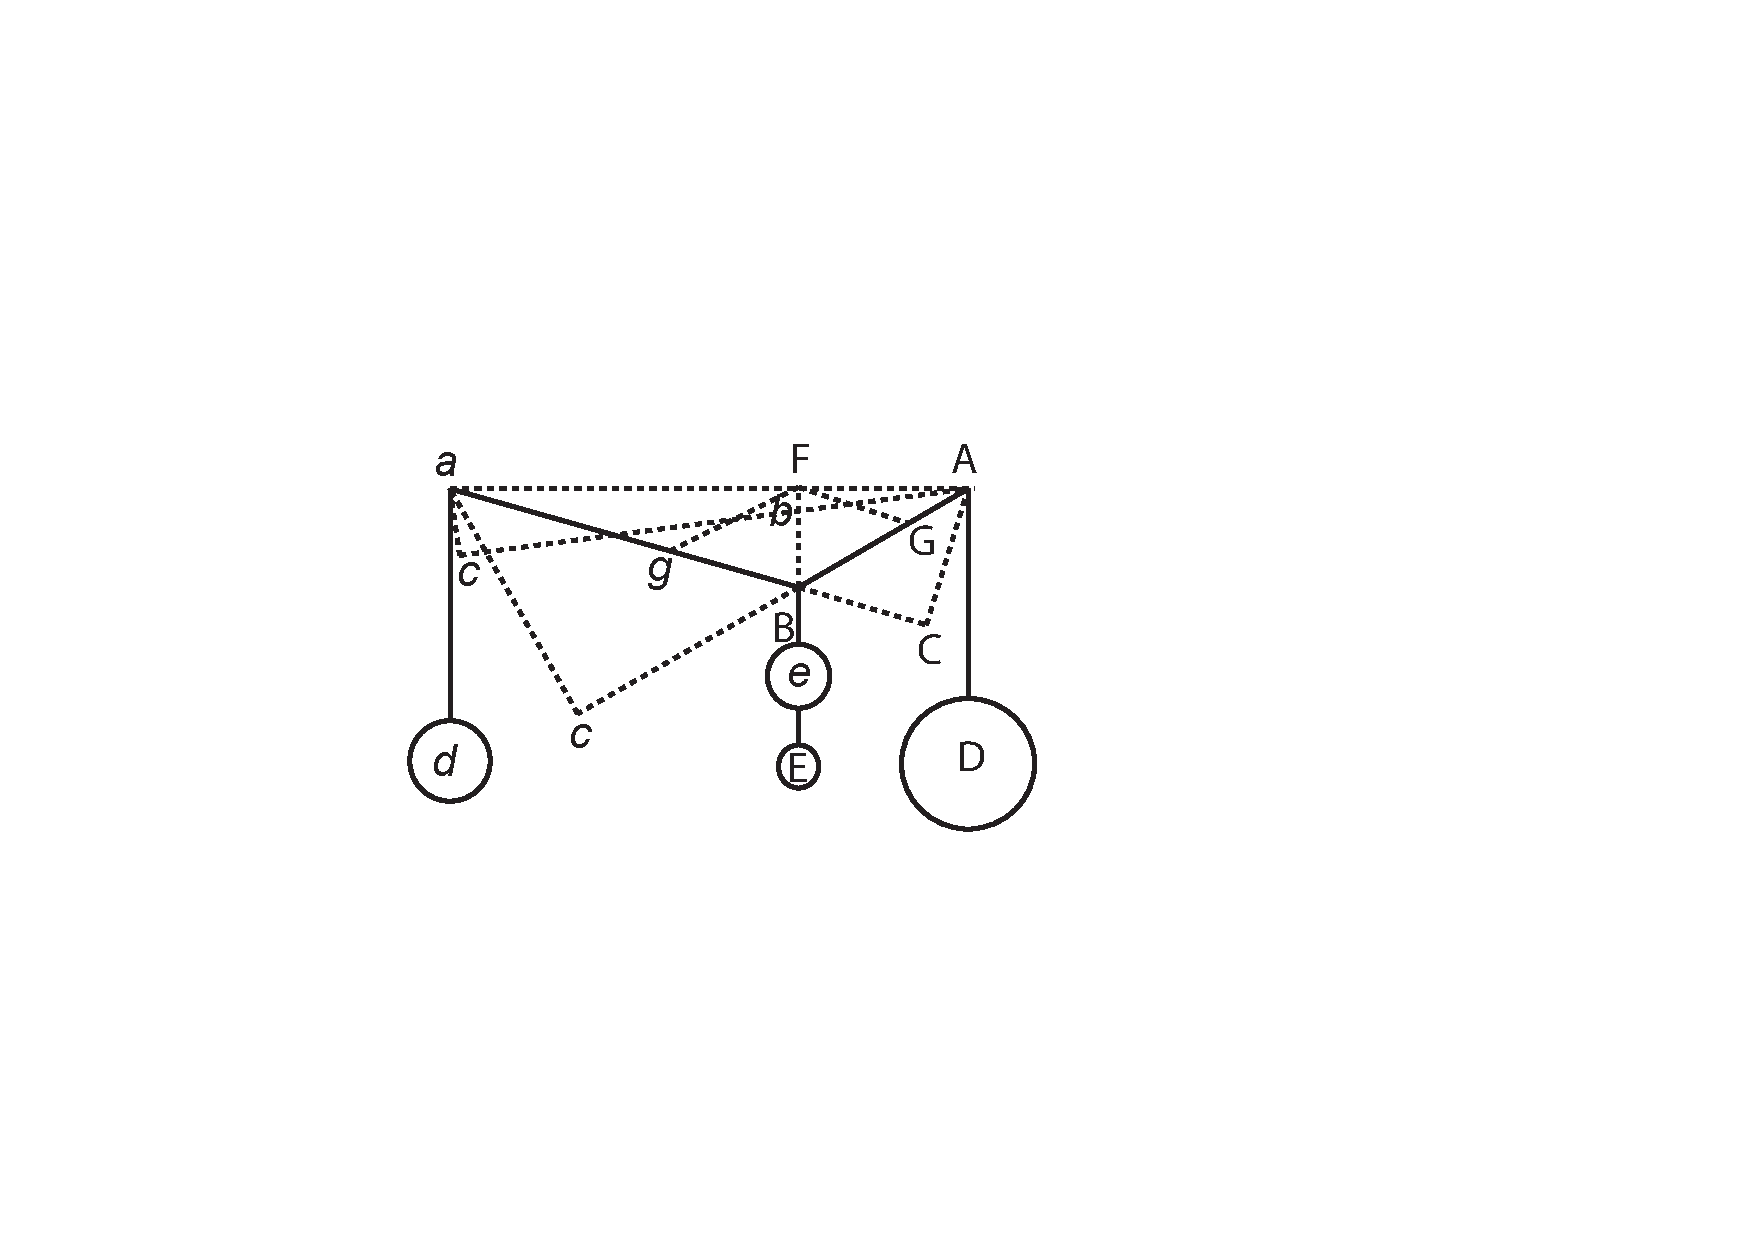
\includegraphics[width=0.45\textwidth]{images/pardies1673-d1.pdf}\\
              \noindent \centering [\textit{Fig. 1}] 
\pend
\vspace{1em}
\count\Afootins=1000
\pstart Pour \setline{8}le prouver, imaginons que les lignes \textit{AC},\edtext{}{\lemma{}\Afootnote{\textit{Am unteren Rand unter Text und Zeichnung}: Si alligata sit chorda in \textit{A}, et una sit trochlea \textit{a}, et agit pondus unum ut \textit{D}, videndum an non sit idem ac si duae essent trochleae duaque pondera aequalia.\vspace{2mm}}} [p. 113] \textit{a c} tombent perpendiculairement sur les cordes \textit{aBC}, \textit{ABc}, prolong\'{e}es s'il en est besoin.
\pend 
\pstart 
[p. 122] Je ne m'arreste pas \`{a} prouver que ces cordes (lors qu'elles ne sont pas paralleles) se doivent croiser en quelque point; car il est assez manifeste que les points \textit{a A} , \textit{o n} sont en mesme \edtext{plan.}{\lemma{}\Afootnote{\textit{Leibniz unterstreicht}: plan. \textit{und schreibt daneben}: rien n'emp\^{e}che qu'on ne les fasse tomber en deux plans differens.}}
\pend
\count\Afootins=1500
 



\chapter[\scriptsize\uppercase{De vi corporum}]{\uppercase{De vi corporum}
\newline\lbrack XXX \textendash\ XXX\rbrack}
\addcontentsline{toc}{chapter}{\thechapter\enskip De vi corporum \lbrack XXX \textendash\ XXX\rbrack}
\vspace{8mm}
    %\begin{ledgroupsized}[r]{120mm}
\footnotesize 
\pstart 
\noindent\textbf{\"{U}berlieferung:}
\pend
\end{ledgroupsized}
\begin{ledgroupsized}[r]{114mm}
\footnotesize 
\pstart \parindent -6mm
\makebox[6mm][l]{\textit{L}}%
Konzept: LH XXXVII 5 Bl. 120. 1 Bl. 2\textsuperscript{o}. 1 \unitfrac{1}{2} S. Wasserzeichen. Papier durch Erhaltungsma{\ss}nahmen gesichert.\\Cc 2, Nr. 00 \pend
\end{ledgroupsized}
%\normalsize
\vspace*{5mm}

\begin{ledgroup}
\footnotesize 
\pstart
\noindent\footnotesize{\textbf{Datierungsgr\"{u}nde}: 
Das Wasserzeichen im Textträger des vorliegenden Stücks ist für den Zeitraum vom Anfang 1674 bis zum Anfang 1675 belegt.}
\pend
\end{ledgroup}

\vspace*{8mm}
\pstart
\noindent
[120~r\textsuperscript{o}]
\pend
\pstart 
\normalsize
\centering De vi\protect\index{Sachverzeichnis}{vis} corporum per motum naturalem\protect\index{Sachverzeichnis}{motus naturalis} \edtext{continuatum}{\lemma{}\Bfootnote{continuatum \textit{erg. L}}} acquisita\\ Ratiocinatio
\pend 
\count\Afootins=1200
\count\Bfootins=1000
\pstart \vspace*{0.5em} 
\noindent Ponatur \edtext{globus \textit{A}}{\lemma{Ponatur}\Bfootnote{\textit{(1)} corpus a \textit{(2)} globus \textit{A} \textit{L}}} labi ex altitudine tanta \textit{ab} quanta sufficiat ad acquirendum impetum\protect\index{Sachverzeichnis}{impetus}, per quem \edtext{\textit{A}}{\lemma{quem}\Bfootnote{\textit{(1)} corpus labens \textit{(2)} \textit{a} \textit{(3)} \textit{A} \textit{L}}} superet \edtext{sphaeram \textit{B} sibi aequalem et aequiponderantem}{\lemma{superet}\Bfootnote{\textit{(1)} corpus sibi aequale et aequiponderans \textit{B} idque \textit{(2)} sphaeram \textit{B} \textit{(a)} similem sibi \textit{(b)} sibi aequalem et aequiponderantem \textit{L}}} \edtext{tanto virium\protect\index{Sachverzeichnis}{vis} excessu ut eam elevare possit}{\lemma{}\Bfootnote{tanto virium\protect\index{Sachverzeichnis}{vis} excessu \textit{(1)} eamque \textit{(2)} ut eam elevare possit \textit{erg.} \textit{L}}} elevet per tantam altitudinem quanta est ipsius sphaerae seu ex \textit{d} \edtext{in \textit{c}. Quod fiet si sphaera labens ex \textit{a} in \textit{b}, impingat in eminentiam \textit{eF} prodeuntem ex chorda \textit{cgh} circa trochleam \textit{g} replicata sphaeramque \textit{B} sustinente. Sed ponamus debere}{\lemma{in \textit{c}.}\Bfootnote{\textit{(1)} Porro numerus sphaerarum \textit{(2)} Sed ad restituenda omnia in statum priorem, \textit{(a)} opus esset \textit{(b)} deberet \textit{(3)} Quod fiet [...] ponamus debere \textit{L}}} elevare integram columnam \edtext{talium}{\lemma{}\Bfootnote{talium \textit{erg.} \textit{L}}} sphaerarum, in recta linea \textit{ab} collocabilium.
\pend
\pstart
Harum sphaerarum numerum appellemus \edtext{$\alpha$}{\lemma{appellemus}\Bfootnote{\textit{(1)} \textit{a} \textit{(2)} $\upsilon$ \textit{(3)} $\xi$ \textit{(4)} $\alpha$ \textit{L}}}. 
\pend
\pstart
Ergo \textit{A} labens ex altitudine \textit{ab} elevabit 1.
\pend 
\pstart
Duplicetur altitudo \textit{ab} erit duplicata altitudo \edtext{l\edtext{apsus\protect\index{Sachverzeichnis}{lapsus} \textit{ae}}{\lemma{lapsus}\Bfootnote{\textit{(1)}\ $a$ \textit{(2)}\ \textit{ae} \textit{L}}}}{\lemma{}\Afootnote{\textit{Über} lapsus $ae$: cum debeat $\alpha$\vspace{-8mm}}} duplicabitur quoque numerus sphaerarum \edtext{elevandarum}{\lemma{}\Bfootnote{elevandarum \textit{erg.} \textit{L}}}. At vero \edtext{quadruplicabuntur vires seu numerus}{\lemma{vero}\Bfootnote{\textit{(1)} quadruplicabitur numerus virium \textit{(2)} quadruplicabuntur vires seu numerus \textit{L}}} sphaerarum elevabilium. Et multiplicata altitudine semper magis multiplicabuntur vires\protect\index{Sachverzeichnis}{vis} quam onus, si quidem vera sunt quae hactenus ab omnibus fere recipiuntur quod scilicet \edtext{gravium impetus crescant}{\lemma{scilicet}\Bfootnote{\textit{(1)} gravia crescant \textit{(2)} gravium impetus crescant \textit{L}}} in duplicata altitudinum ratione. Ergo denique superabitur onus a viribus\protect\index{Sachverzeichnis}{vis}, ac proinde assumta altitudine sufficienti, \edtext{sequetur plena machinae restitutio}{\lemma{sufficienti,}\Bfootnote{\textit{(1)} sequi omnimodam plenam machinae restitutionem\protect\index{Sachverzeichnis}{machinae restitutio|textit} \textit{(2)} sequetur plena machinae restitutio \textit{L}}}, quae altitudo an in praxi haberi possit nihil refert ad institutum, sufficit demonstrari posse, aut restitutionem perfectam\protect\index{Sachverzeichnis}{restitutio perfecta} ex natura motus sequi, aut ejus proportiones\protect\index{Sachverzeichnis}{proportio} receptas exactas non esse. Quod credere malim. \setline{6}Calculus hic erit:
\pend
\count\Afootins=1200
\count\Bfootins=1200
\pstart
\vspace*{1em}
\noindent
\begin{tabular}{ccccll}
$A$ 
{labens\renewcommand*{\raggedleftmarginnote}{} \reversemarginpar\marginnote{\scriptsize\hspace{46mm}10}}
ex &elevabit in altitudinem sui&cum debeat elevare&&&\\
altitudine&sphaeras&sphaeras&id est e.g.&&\\
1&1&$\alpha$ 1&10&9&8\\
2&4&$\alpha$ 2&20&18&16\\
3&9&$\alpha$ 3&30&27&24\\
{4\renewcommand*{\raggedleftmarginnote}{}\reversemarginpar\marginnote{\scriptsize\hspace{46mm}15}}
&16&$\alpha$ 4&40&36&32\\
5&25&$\alpha$ 5&50&45&40\\
6&36&$\alpha$ 6&60&54&48\\
7&49&$\alpha$ 7&70&63&65\\
8&\uline{64}&$\alpha$ 8&80&72&\uuline{64}\\
{9\renewcommand*{\raggedleftmarginnote}{}\reversemarginpar\marginnote{\scriptsize\hspace{46mm}20}}
&\uline{81}&$\alpha$ 9&90&\uuline{81}&72\\
10&\uline{100}&$\alpha$ 10&\uuline{100}&90&80\\
\end{tabular}
%\begin{tabular}{ccccll}
%$A$ labens ex &elevabit in altitudinem sui&cum debeat elevare&&&\\
%altitudine&sphaeras&sphaeras&id est e.g.&&\\
%1&1&$\alpha$ 1&10&9&8\\
%2&4&$\alpha$ 2&20&18&16\\
%3&9&$\alpha$ 3&30&27&24\\
%4&16&$\alpha$ 4&40&36&32\\
%5&25&$\alpha$ 5&50&45&40\\
%6&36&$\alpha$ 6&60&54&48\\
%7&49&$\alpha$ 7&70&63&65\\
%8&\uline{64}&$\alpha$ 8&80&72&\uuline{64}\\
%9&\uline{81}&$\alpha$ 9&90&\uuline{81}&72\\
%10&\uline{100}&$\alpha$ 10&\uuline{100}&90&80\\
%\end{tabular}
\pend
\pstart
\vspace*{1em}
Si \setline{22}ergo numerus [$\alpha$]\edtext{}{\Bfootnote{a\textit{\ L \"{a}ndert Hrsg.}}} ponatur esse 10. decuplicanda est altitudo prima. Si \edtext{9.}{\lemma{Si}\Bfootnote{\textit{(1)} novem \textit{(2)} 9. \textit{L}}}, noncuplicanda. Et generaliter posito incremento\protect\index{Sachverzeichnis}{incrementum} impetus\protect\index{Sachverzeichnis}{impetus} in duplicata ratione spatiorum \edtext{si multiplicetur}{\lemma{si}\Bfootnote{\textit{(1)} multiplicanda est \textit{(2)} multiplicetur \textit{L}}} altitudo 1. per numerum sphaerarum [$\alpha$]\edtext{}{\Bfootnote{a\textit{\ L \"{a}ndert Hrsg.}}}. Sequetur restitutio perfecta\protect\index{Sachverzeichnis}{restitutio perfecta}; \edtext{ex hypothesi recepta}{\lemma{perfecta;}\Bfootnote{\textit{(1)} ex vulgari hypothesi \textit{(2)} ex hypothesi recepta \textit{L}}} incrementi\protect\index{Sachverzeichnis}{incrementum}. Instituenda hic experimenta\protect\index{Sachverzeichnis}{experimentum}: (1) ex qua altitudine labens corpus datum possit elevare aliud datum sibi aequale, inaequale, aequiponderans, \edtext{aut non\hfill aequiponderans}{\lemma{}\Bfootnote{aut non aequiponderans \textit{erg. L}}},\hfill simile\hfill dissimile,\hfill possit\hfill elevare\hfill in\hfill \textso{altitudinem quantam}.
\pend
\pstart\noindent
\centering
%\begin{wrapfigure}[24]{l}{0.45\textwidth} 
%\vspace{-4mm}
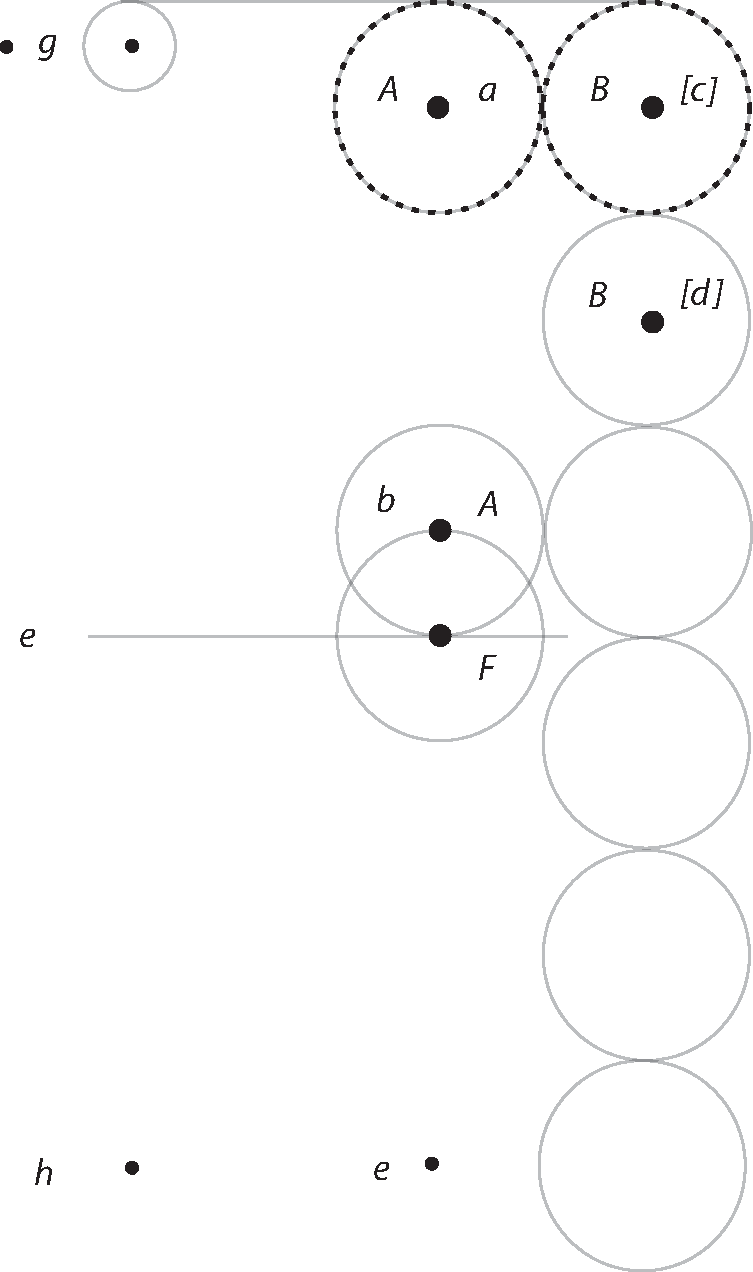
\includegraphics[trim = 0mm -5mm 0mm 0mm, clip, width=0.45\textwidth]{images/lh03705_120r-d1.pdf}\\
%\vspace{0.5em}
             \noindent \centering [\textit{Fig. 1, tlw. Blindzeichnung}] 
%\end{wrapfigure}
\pend
\vspace{1em}
\pstart\noindent Certum \setline{1}est enim corpus labens ex quantulacunque altitudine elevare posse aequiponderans quiescens, sed \edtext{}{\lemma{}\Bfootnote{sed \textbar\ et \textit{gestr.} \textbar\ in \textit{L}}}in altitudinem exiguam.\\
(2) Experiendum quanta altitudine opus sit, ut corpus parvum labens levet corpus magnum sensibiliter in altitudinem quantulamcumque.
\\
(3) Quamdiu duret impetus\protect\index{Sachverzeichnis}{impetus} post concursum seu quamdiu corpus unum alteri ob lapsum praeponderet, quod alioqui non praeponderaret.
\\
(4) Quanta sit resistentia aeris\protect\index{Sachverzeichnis}{resistentia aeris} et an aeris resistentia\protect\index{Sachverzeichnis}{resistentia aeris} crescat cum descensu.
\\
(5) An non incrementum\protect\index{Sachverzeichnis}{incrementum} gravium sit continue decrescens, quod mihi probare posse videor ac sphaera labens elevabit integram columnam sphaerarum sibi aequalium per totam lapsus\protect\index{Sachverzeichnis}{lapsus} altitudinem dispositarum, atque ita ipsa labens subintrabit in locum ultimae, summa autem labi incipiet sequeturque machinae restitutio\protect\index{Sachverzeichnis}{restitutio machinae} in statum priori per omnia similem, aut necesse est doctrinam receptam de incremento\protect\index{Sachverzeichnis}{incrementum} motus gravium\protect\index{Sachverzeichnis}{motus gravium} non satis firmo fundamento niti progressionemque ejus esse non uniformem, sed ut mihi \edtext{probabile videtur decrescentem}{\lemma{mihi}\Bfootnote{\textit{(1)} videtur decrescentem \textit{(2)} probabile videtur decrescentem \textit{L}}}. [120~v\textsuperscript{o}]\\
(6) An \edtext{corpus majus}{\lemma{An}\Bfootnote{\textit{(1)} ex quanto \textit{(2)} majore \textit{(3)} corpus m \textit{(4)} corpus majus \textit{L}}} ex minore, majore, an eadem altitudine lapsum elevet corpus sibi aequiponderans et aequale in altitudinem corporis sui, quam corpus minus elevat aliud \edtext{sibi aequiponderans}{\lemma{}\Bfootnote{sibi aequiponderans \textit{erg.} \textit{L}}} minus. Meretur hoc inprimis observari ducet enim nos in intimas impetus\protect\index{Sachverzeichnis}{impetus} hujus proportiones\protect\index{Sachverzeichnis}{proportio}.
\pend
\pstart 
Sunto duo corpora \edtext{homogenea}{\lemma{}\Bfootnote{homogenea \textit{erg. L}}} aequiponderantia et aequalia gravia et magna. Sunto duo alia levia et parva. Quaestio est an utrobique eadem altitudine lapsus\protect\index{Sachverzeichnis}{lapsus} opus sit, ut labens elevet quiescens in altitudinem corporis sui, aut in altitudinem datam; an \edtext{potius}{\lemma{an}\Bfootnote{\textit{(1)} non \textit{(2)} potius \textit{L}}} majore opus sit, \edtext{aut an}{\lemma{sit,}\Bfootnote{\textit{(1)} an vero \textit{(2)} aut an \textit{L}}} minore, et qua proportione\protect\index{Sachverzeichnis}{proportio}.
\pend
%\newpage
\pstart 
(7) An resistentia corporum\protect\index{Sachverzeichnis}{resistentia corporum} \edtext{lapsum excipientium}{\lemma{}\Bfootnote{lapsum excipientium \textit{erg.} \textit{L}}} crescat ut vis\protect\index{Sachverzeichnis}{vis} labentium. Pone corpus $a$ \edtext{impingens}{\lemma{$a$}\Bfootnote{\textit{(1)} labens \textit{(2)} impingens \textit{L}}} in $b$ \edtext{aequiponderans aut praeponderans}{\lemma{}\Bfootnote{aequiponderans aut praeponderans \textit{erg.} \textit{L}}} id superare per \edtext{aliquod}{\lemma{per}\Bfootnote{\textit{(1)} datum \textit{(2)} aliquod \textit{L}}} temporis spatium, donec impetus\protect\index{Sachverzeichnis}{impetus} evanescat, et $b$ restituat se in aequiponderationem, aut praeponderationem, quaeritur an durante isto temporis spatio impetus\protect\index{Sachverzeichnis}{impetus} impingentis decresceat seu evanescere incipiat uniformiter, an difformiter et qua proportione. Et an ipsum corpus resistens magis resistat momento\protect\index{Sachverzeichnis}{momentum} aliquo sequente quam antecedente.
\pend
\pstart 
Sed hic examinandum esset quid aeris resistentia\protect\index{Sachverzeichnis}{resistentia aeris} conferat an ipsa quoque cum impetu\protect\index{Sachverzeichnis}{impetus} lapsus\protect\index{Sachverzeichnis}{lapsus} \edtext{labentis}{\lemma{}\Bfootnote{labentis \textit{erg. L}}} crescat.
\pend
\pstart 
Ante omnia autem experiendum est quanta altitudine lapsus\protect\index{Sachverzeichnis}{lapsus} opus habeat corpus, ad elevandum aliud aequiponderans in altitudinem corporis. Et quae sit ratio altitudinis lapsus\protect\index{Sachverzeichnis}{lapsus}. Si corpora aequiponderantia sunt magna, aut non magna quidem, gravia tamen magis; ad altitudinem lapsu minorum.
\pend
\pstart  
Quibus aliisque quae nunc enumerare prolixum foret constitutis doctrina motuslapsus\protect\index{Sachverzeichnis}{doctrina motus gravium} gravium\protect\index{Sachverzeichnis}{motus gravium} in majore luce constituetur.
\pend
\count\Afootins=1500
\count\Bfootins=1500

    %\input{gesamttex/edit/LH037_05_120v.tex}


\chapter[\scriptsize\uppercase{R\`{e}gle pour calculer la force d' une machine}]{\uppercase{R\`{e}gle pour calculer la force d' une machine}
\newline\lbrack Fr\"{u}hjahr \textendash\ Herbst 1673\rbrack}
\addcontentsline{toc}{chapter}{\thechapter\enskip R\`{e}gle pour calculer la force d' une machine \lbrack Fr\"{u}hjahr \textendash\ Herbst 1673\rbrack}
\vspace{8mm}
%    \input{gesamttex/edit/LH035_10_9_001-4_intro.tex}

\vspace{12mm}
\section[\scriptsize\uppercase{R\`{e}gle pour calculer la force d'une machine. Premier essai}]{\uppercase{R\`{e}gle pour calculer la force d'une machine. Premier essai}
\newline\lbrack Fr\"{u}hjahr \textendash\ Sommer 1673\rbrack}
\addcontentsline{toc}{section}{\thesection\enskip R\`{e}gle pour calculer la force d'une machine. Premier essai \lbrack Fr\"{u}hjahr \textendash\ Sommer 1673\rbrack}
\vspace{4mm}
%    \begin{ledgroupsized}[r]{120mm}
\footnotesize 
\pstart 
\noindent\textbf{\"{U}berlieferung:}
\pend
\end{ledgroupsized}
\begin{ledgroupsized}[r]{114mm}
\footnotesize 
\pstart \parindent -6mm
\makebox[6mm][l]{\textit{L}}Aufzeichnung:
LH XXXV 10, 9 Bl. 3-4. 1 Bog. 2\textsuperscript{o}.
\nicefrac{1}{2} Sp. auf Bl. 3~r\textsuperscript{o} links oben.
Der übrige Text auf Bl. 3~r\textsuperscript{o} gehört zu N.~28\textsubscript{5}. % = LH035,10,9 Bl. 3r_2 = Regula de vi ponderis
Der Bog. überliefert ferner N.~28\textsubscript{1}, % = LH035,10,9 Bl. 3v_1 = Règle pour calculer la force d'une machine 1
N.~28\textsubscript{2} % = LH035,10,9 Bl. 3v_2 = Règle pour calculer la force d'une machine 2
und N.~28\textsubscript{6}.% = LH035,10,9 Bl. 4 = De determinatione machinae virium
\\%
Cc 2, Nr. 1191 (tlw.)
\pend
\end{ledgroupsized}
%
\vspace*{5mm}
\begin{ledgroup}
\footnotesize 
\pstart
\noindent\footnotesize{\textbf{Datierungsgr\"{u}nde}: Das vorliegende Stück befindet sich zusammen mit Unterstücken von N. 28 %
% = LH035,10,9 Bl. 1-4 = Règle pour calculer la force d'une machine
auf einem Bogen und dürfte daher zeitnah zu diesen letzteren entstanden sein.
Die Datierung von % = LH035,10,9 Bl. 1-4 = Règle pour calculer la force d'une machine
N.~28~--~zweite Hälfte 1674 bis Anfang 1675 -- wird demgemäß auch für das vorliegende Stück übernommen.}
\pend
\end{ledgroup}
%
\vspace*{8mm}
\pstart 
\normalsize
\begin{wrapfigure}[13]{l}{0.38\textwidth}  
\vspace{-5mm}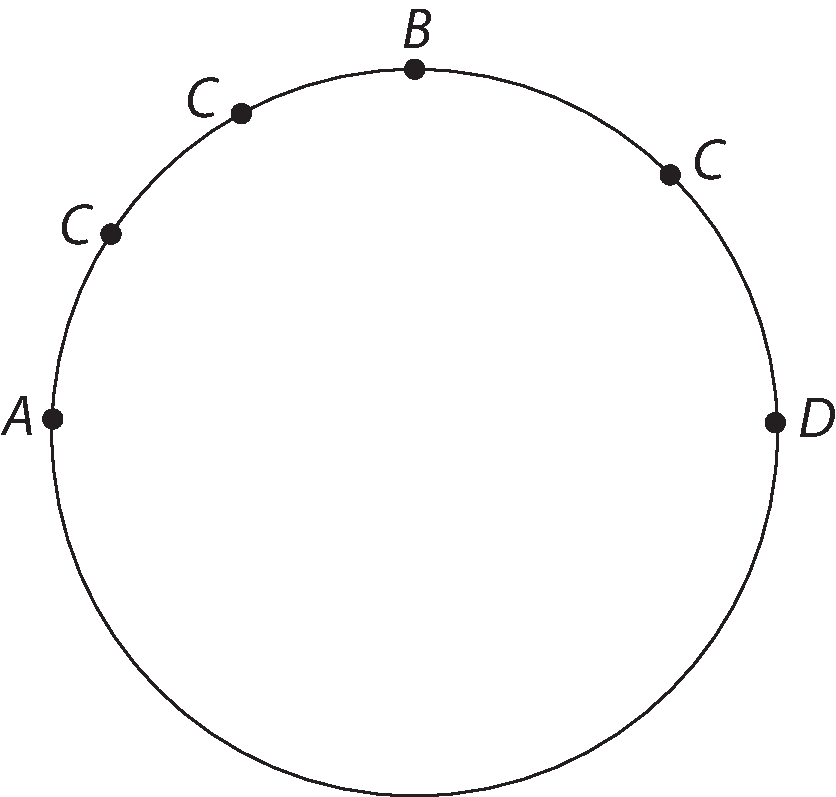
\includegraphics[trim = 0mm -3mm -4mm 0mm, clip, width=0.38\textwidth]{images/lh0351009_003r-d1.pdf}\\
\centering[\textit{Fig. 1}]
\end{wrapfigure}
\noindent%
% [3~r\textsuperscript{o}]
[3~r\textsuperscript{o}] Experiundum est, an Magnes\protect\index{Sachverzeichnis}{magnes} habeat sphaeram activitatis\protect\index{Sachverzeichnis}{sphaera activitatis} determinatam, id est, pone Magnetem elevare posse certum ferri\protect\index{Sachverzeichnis}{ferrum} pondus\protect\index{Sachverzeichnis}{pondus} ex distantia data; ita ut aucta distantia elevare amplius non possit; quaeritur an aucta distantia omnino non agat in ferrum\protect\index{Sachverzeichnis}{ferrum} illud. Hoc ita experiri licet: Pone ferrum\protect\index{Sachverzeichnis}{ferrum} illud in fundo vasis\protect\index{Sachverzeichnis}{vas} aqua\protect\index{Sachverzeichnis}{aqua} pleni esse; distantia a magnete\protect\index{Sachverzeichnis}{magnes} superposito, majore paulo quam ut ab eo attrahi possit. Jam infigamus illud ferrum\protect\index{Sachverzeichnis}{ferrum} rei cuidam levi ut suberi\protect\index{Sachverzeichnis}{suber}; ita tamen ut pondus\protect\index{Sachverzeichnis}{pondus} ferri\protect\index{Sachverzeichnis}{ferrum} praeponderet levitati suberis\protect\index{Sachverzeichnis}{suber}; id est ut maneat in fundo: Experiundum erit admoto magnete, an frustum illud ex ferro\protect\index{Sachverzeichnis}{ferrum} et subere\protect\index{Sachverzeichnis}{suber} elevare possit; nam si elevat; sequitur sphaeram illam activitatis\protect\index{Sachverzeichnis}{sphaera activitatis} non fuisse determinatam; sed magnetem\protect\index{Sachverzeichnis}{magnes} egisse in ferrum\protect\index{Sachverzeichnis}{ferrum} etsi non satis fortiter, quod nunc apparet; quoniam levius redditum attolit. Sin minus patet magnetem habere sphaeram activitatis\protect\index{Sachverzeichnis}{sphaera activitatis} determinatam; ultra quam omnino non agat.
\pend
\pstart
Idem sic quoque facilius indagari potest; examinando an sit distantia quaedam assignabilis; ex qua magnes\protect\index{Sachverzeichnis}{magnes} frustum ferri\protect\index{Sachverzeichnis}{ferrum} parvum elevet, majus quod ex minore elevaret, non \edtext{elevaret. 
Hinc patebit an magnes eadem vi agat in magna parva distantia.}{\lemma{\hspace{1.8mm}27-S. 51.1}\killnumber\Bfootnote{elevaret.\ \textbar\ Hinc [...] distantia. \textit{erg.}\ \textbar\ \textit{(1)}\ Si duo \textit{(2)}\ Si sit \textit{L}}} \pend
\newpage
\pstart
Si sit pila\protect\index{Sachverzeichnis}{pila} ferrea, et duobus magnetibus\protect\index{Sachverzeichnis}{magnes} in oppositis punctis $\displaystyle A. D$, opposito modo fricetur, ponendo magnetes esse aequales, destruetur effectus mutuo. Jam examinandum est, quid fiat, si fricetur simul in $\displaystyle A$ et $\displaystyle C$ pro varia anguli ratione.
\pend
\pstart
Experiendum an eundem effectum faciat annulus\protect\index{Sachverzeichnis}{annulus} ferreus, quem pila\protect\index{Sachverzeichnis}{pila} aut acus\protect\index{Sachverzeichnis}{acus}: idem quae aliae a figuris varietates. Experiendum an mutatio oriatur, certis partibus in magnete\protect\index{Sachverzeichnis}{magnes} \edtext{aut pila\protect\index{Sachverzeichnis}{pila}}{\lemma{aut pila}\Bfootnote{\textit{erg. L}}}
igne mutilibus redditis, v.g. aequatore\protect\index{Sachverzeichnis}{aequator}; et aliis; item quid fiat uno polo\protect\index{Sachverzeichnis}{polus} ignito, altero \edtext{relicto.}{\lemma{altero}\Bfootnote{\textit{(1)}\ destructo \textit{(2)}\ relicto \textit{L}}}
\pend
\pstart
De ratione faciendi compassum\protect\index{Sachverzeichnis}{compassus} nauticum maximum ad minuta usque secunda divisum. Acus\protect\index{Sachverzeichnis}{acus} magneticae in extremitate $\displaystyle M.$
\pend
\pstart
De modo inclinationem\protect\index{Sachverzeichnis}{inclinatio} et declinationem\protect\index{Sachverzeichnis}{declinatio} ad regulam revocandi, in terra\protect\index{Sachverzeichnis}{terra}: per $\displaystyle P$ parallelos et meridianos.
\pend
\pstart
Magnetis\protect\index{Sachverzeichnis}{magnes} vis attractiva\protect\index{Sachverzeichnis}{vis attractiva} $c+g+h$, pondus\protect\index{Sachverzeichnis}{pondus} \edtext{[pilulae]}{\lemma{pilylae}\Bfootnote{\textit{L \"{a}ndert Hrsg.}}} \edtext{ferro\protect\index{Sachverzeichnis}{ferrum} gravis}{\lemma{ferro}\Bfootnote{\textit{(1)}\ imbuit \textit{(2)}\ gravis \textit{L}}} $g+h$. $\displaystyle h$ pondus\protect\index{Sachverzeichnis}{pondus} aquae\protect\index{Sachverzeichnis}{aqua} paris spatii[,] $\displaystyle c+g+h+d$ 
pondus\protect\index{Sachverzeichnis}{pondus} ipsius magnetis\protect\index{Sachverzeichnis}{magnes}[,] ex centro $\displaystyle E,$ radio $\displaystyle EC.$
Hactenus figura data, fiat nova.
\pend 


\vspace{12mm}
\section[\scriptsize\uppercase{R\`{e}gle pour calculer la force d'une machine. Deuxi\`{e}me essai}]{\uppercase{R\`{e}gle pour calculer la force d'une machine. Deuxi\`{e}me essai}
\newline\lbrack Fr\"{u}hjahr \textendash\ Sommer 1673\rbrack}
\addcontentsline{toc}{section}{\thesection\enskip R\`{e}gle pour calculer la force d'une machine. Deuxi\`{e}me essai \lbrack Fr\"{u}hjahr \textendash\ Sommer 1673\rbrack}
\vspace{4mm}
%    \begin{ledgroupsized}[r]{120mm}
\footnotesize 
\pstart 
\noindent\textbf{\"{U}berlieferung:}
\pend
\end{ledgroupsized}
\begin{ledgroupsized}[r]{114mm}
\footnotesize 
\pstart \parindent -6mm
\makebox[6mm][l]{\textit{L}}%
Konzept: LH XXXV 10, 9 Bl. 3-4. 1 Bog. 2\textsuperscript{o}. 1\,\nicefrac{1}{3} Sp. auf Bl.~3~r\textsuperscript{o}.
Der Bogen überliefert ferner N.~28\textsubscript{1}, N.~28\textsubscript{2}, N.~28\textsubscript{6} und N.~5.
%LH35,10,09 Bl. 3r = Demonstratio geometrica de magnetis sphaera
\\
Cc 2, Nr. 1191 (tlw.)
\pend
\end{ledgroupsized}

%%\normalsize
%\vspace*{5mm}
%\begin{ledgroup}
%\footnotesize 
%\pstart
%\noindent\footnotesize{\textbf{Datierungsgr\"{u}nde}: bisher keine absolute Datierung, nur Einordnung in Sequenz zur Kraft am Rad erfolgt}
%\pend
%\end{ledgroup}
 
\vspace*{8mm}
\count\Bfootins=1200
\count\Cfootins=1200
\pstart 
\normalsize
\noindent[3~r\textsuperscript{o}]\edtext{}{\lemma{\hspace{1.8mm}[\textit{Fig. 1}]}\killnumber\Cfootnote{Die Parallele \textit{ATR} ist gestrichen. \hspace{7cm}}} Centro $L$ esto \edtext{circulus $LN$ intervalla $LQ$ diametri}{\lemma{circulus $LN$} \Bfootnote{\textit{(1)}\ intervalla $LP$ in radio item alia minora \textit{(2)}\ intervalla $LQ$ \textit{(a)}\ in circul \textit{(b)}\ diametri \textit{L}}} portiones inter se aequales $AB$, $AB \hspace{0.5mm}\sqcap\hspace{0.5mm} TS\hspace{0.5mm} \sqcap \hspace{0.5mm}\beta$ tangens respondens intercepta: $NMO$ vel $RGS$. Sit triangulum $STR$, ducatur $TE$ parallela $LG$ erit ang. $GLF\hspace{1mm} \sqcap$ angulo $ETS$. Ergo ang. $TSR \, \sqcap \, \text{angulo} \, FGL$. Ergo $RS$ ad $TS$ seu $RS$ \edtext{ad $\beta$ ut $LG \sqcap a$ ad}{\lemma{ad $\beta$}\Bfootnote{ \textit{(1)}\ ut $a$ ad \textit{(2)}\ ut $LG \sqcap a$ ad \textit{ L}}} $FG \sqcap y$ et erit \rule[-4mm]{0mm}{10mm}$RS \sqcap \displaystyle\frac{a \beta}{y}$.
\pend
\vspace{1em}
\pstart
\noindent
%\begin{wrapfigure}[14]{l}{0.42\textwidth}
%\vspace{-5mm}
\setline{6}\centering
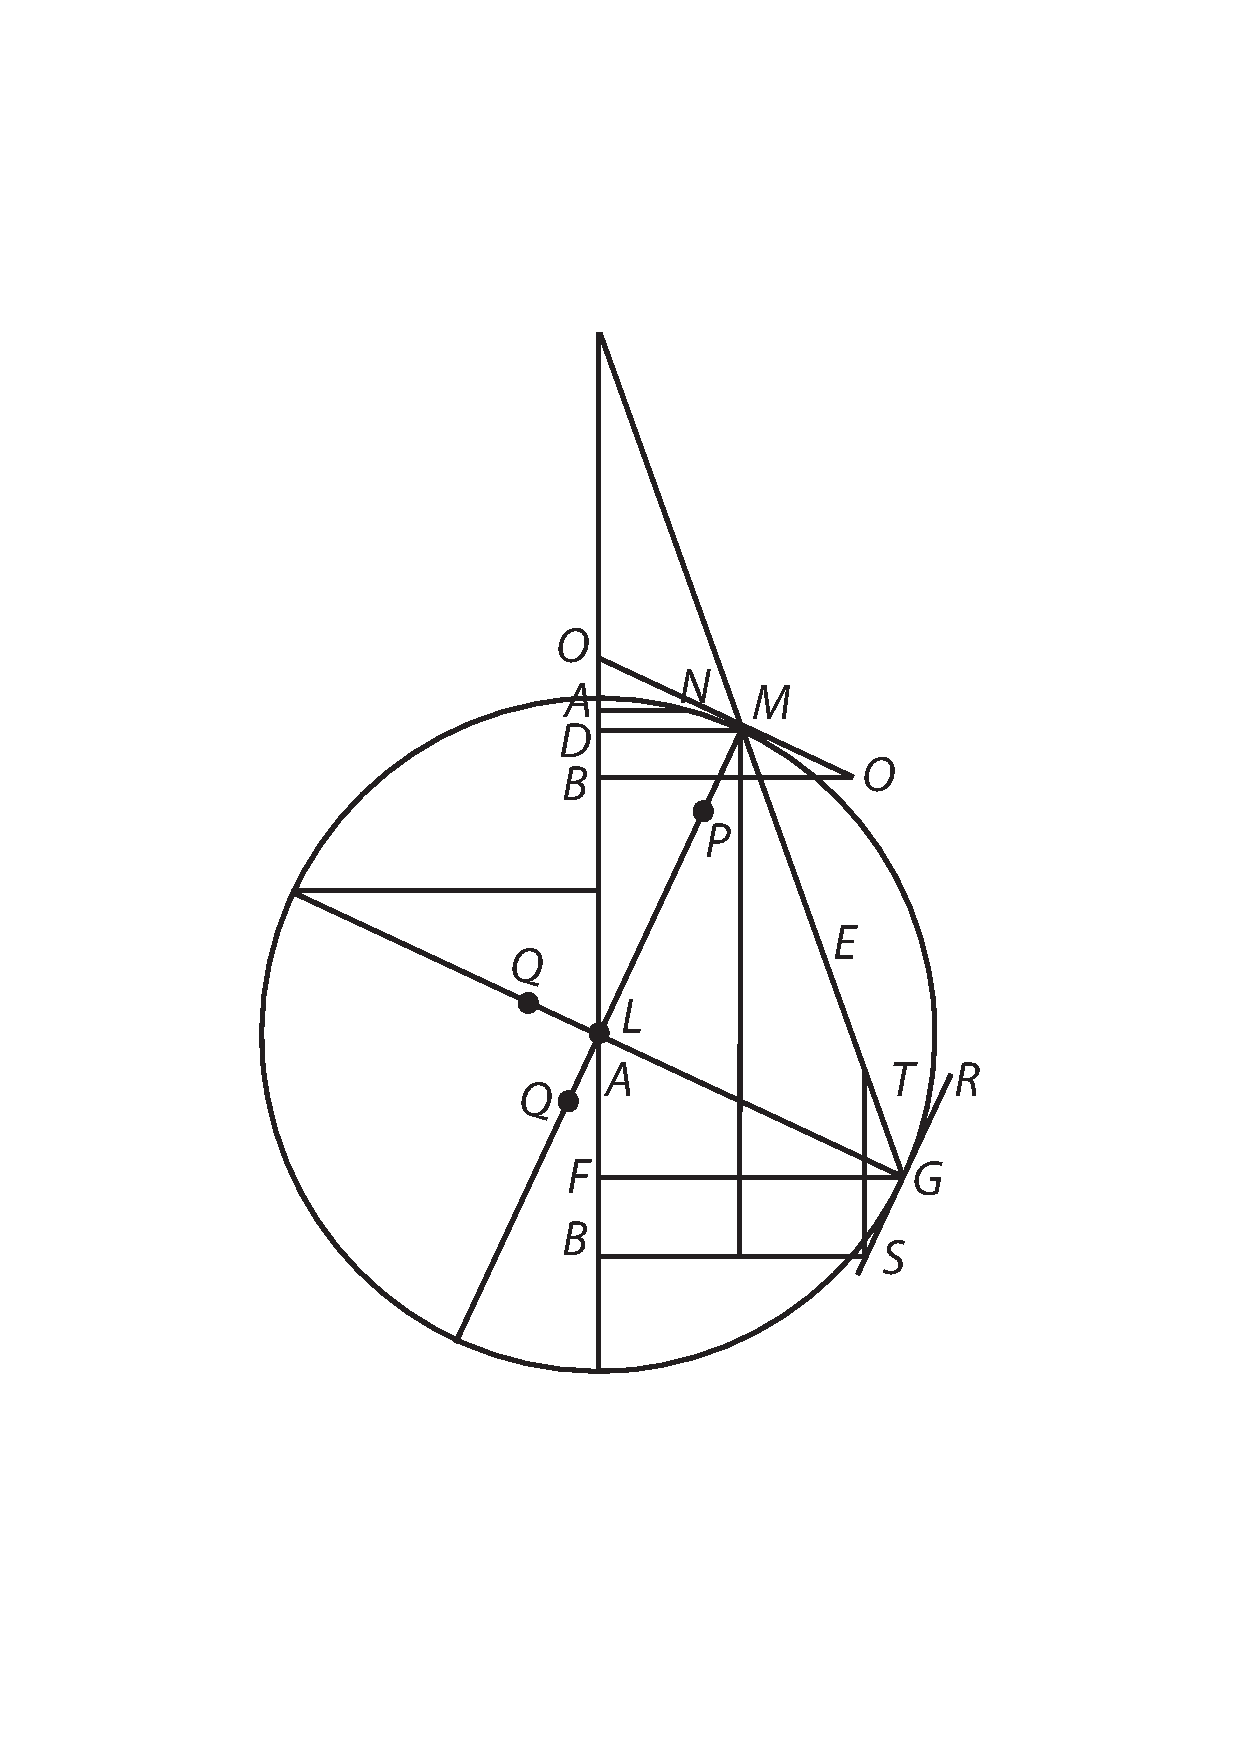
\includegraphics[trim = 0mm -2mm 0mm 0mm, clip, width=0.4\textwidth]{images/lh0351009_003r_2-d2.pdf}\\
\noindent \centering [\textit{Fig. 1}] 
%\end{wrapfigure}
\pend
\pstart Itaque vis ponderis\protect\index{Sachverzeichnis}{vis ponderis} descendentis in circuli circumferentia, erit ad vim ejusdem ponderis descendentem recta, in ratione $\beta$ ad \rule[-4mm]{0mm}{10mm}$\displaystyle\frac{a \beta}{y}$ sive ut $y$ ad $a$, sive ut sinus ad \rule[-4mm]{0mm}{10mm}\edtext{radium, et pone $LQ \hspace{1mm} \sqcap \hspace{1mm}\displaystyle\frac{a^2}{b}$ erit vis ponderis in $LQ \hspace{1mm}\sqcap \hspace{1mm}\displaystyle\frac{y}{b}$. Jam}{\lemma{radium,} \Bfootnote{\textit{(1)}\ pone jam $a \sqcap 1$. \textit{(2)}\ et pone $LQ \sqcap \displaystyle\frac{a^2}{b}$ erit vis ponderis in $LQ \sqcap \displaystyle\frac{y}{b}$. Jam \textit{L}}}\rule[-4mm]{0mm}{10mm} cum duae sint $y$, una $\sqcap \hspace{1mm}DM$ altera $\sqcap \hspace{1mm}LG$ quarum puncta $M.\ G$ quadrante distant, relatione quadam perpetua explicandae rectae $DM$, et $LG$, quae aequatione quadam sive regula exprimatur. Nimirum recta $MG$ est data et constans $\surd{2a^2}$ seu $a\surd{2}$. 
\pend 
\pstart Datur $LG \sqcap a$. Ponamus $LF \sqcap x$ et $FG \sqcap z$. Fiet: $a^2-x^2 \sqcap z^2$. Porro datur \edtext{$DM \sqcap y$}{\lemma{$DM \sqcap y$}\Cfootnote{Hiermit $y$ neu gesetzt. Vorher galt: $FG \sqcap y$.}} et $DL \rule[-4mm]{0mm}{10mm} \sqcap \sqrt{a^2 - y^2}$ ergo $DF$ sive $MK \sqcap \sqrt{a^2 - y^2} + x$ et $KG^2 \sqcap \ovalbox{2} a^2 \ovalbox{$-a^2$} -y^2 -x^2 -2x \sqrt{a^2 - y^2}$.\edtext{}{\lemma{$KG^2$ [...] $-2x \sqrt{a^2 - y^2}$}\Cfootnote{Korrekter Wert für $KG^2$ ist $y^2$. Den Fehler berichtigt die Gleichung $z\, \sqcap\, (\alpha \omega \alpha \omega) \sqrt{y^6 - y^4 + y^2 + 1} (\omega \omega \alpha \alpha) \displaystyle\frac{y^3}{a^2}$ auf S.~\pageref{LH0351009_003r_Gleichung}.}} 
\pend
\vspace{1.5em}
\pstart
\begin{center}                    
\setline{6}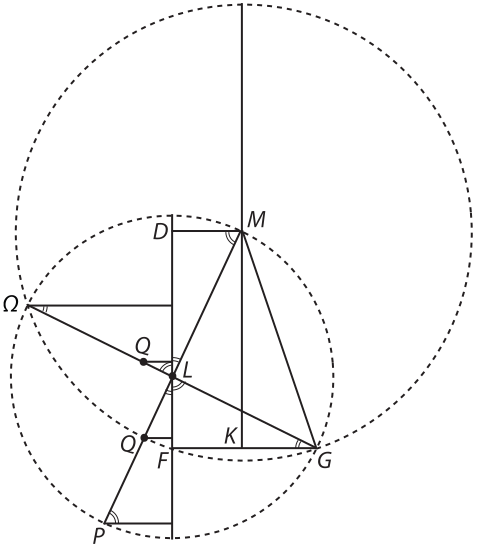
\includegraphics[width=0.5\textwidth]{images/lh0351009_003r_2-d4.pdf}\\
\end{center}
\noindent \centering [\textit{Fig. 2}]
\pend
\newpage
\pstart \noindent Et fiet: seu \rule[-4mm]{0mm}{10mm}$KG \sqcap \displaystyle\efrac{\sqrt{+a^2 - x^2 - 2x \sqrt{a^2 - y^2}}}{-y^2\hfill}$ et $FG$ erit \rule[-4mm]{0mm}{10mm}$\sqcap \displaystyle\efrac{\sqrt{a^2 - x^2 - 2x \sqrt{a^2 - y^2}}}{-y^2\hfill} (\PsMs) y \sqcap z$ sive \rule[-4mm]{0mm}{10mm}$\displaystyle\efrac{+a^2 - x^2 - 2 \sqrt{a^2 - y^2} x}{-y^2 \hfill}\sqcap z^2 (\MsPs) 2yz + y^2$ sive $a^2-y^2$ appellando per compendium $\omega^2$, fiet: \rule[-4mm]{0mm}{10mm}\edtext{aequatio}{\lemma{fiet:} \Bfootnote{\textit{(1)}\ $\omega^2-x^2-2\omega$ \textit{(2)}\ aequatio \textit{L}}} $\displaystyle\efrac{z^2 + x^2 (\MsPs) 2yz + 2\omega x - a^2}{\hfill +2y^2}\sqcap 0$. Jam supra $z^2x^2-a^2 \sqcap 0$. Ergo conferendo posteriorem ex priore, fiet: $(\MsPs) \cancel{2}yz + \cancel{2}\omega x + \cancel{2}y^2 \sqcap 0$. \edtext{Ideoque}{\lemma{$\cancel{2}y^2 \sqcap 0$}\Bfootnote{\textit{(1)} sive $z\sqcap \displaystyle\frac{\cancel{2}\omega x + \cancel{2}y^2}{\cancel{2}y}$ \textit{(2)} Ideoque \textit{ L}}} $x\sqcap \displaystyle\frac{\MsPs \hspace{0.5mm} yz - y^2}{\omega}$\rule[-4mm]{0mm}{10mm} et \rule[-4mm]{0mm}{10mm}$x^2\sqcap \displaystyle\frac{-y^2 z^2 (\PsMs) 2y^3 z+y^4}{a^2 - y^2}$ \rule[-4mm]{0mm}{10mm}quem valorem substituendo in aequatione $z^2+x^2-a^2 \sqcap 0$ fiet: $z^2 a^2 \ovalbox{$-z^2y^2, +y^2z^2$} (\PsMs) 2y^3z + y^4, -a^4 - y^2 a^2 \sqcap 0$\edtext{}{\lemma{$- y^2 a^2$}\Cfootnote{Das Vorzeichen des Terms muss positiv sein.}} \edtext{fingendo}{\lemma{}\Bfootnote{fingendo \textit{erg. L}}} $y^4-a^2y^2-a^4$, \rule[-4mm]{0mm}{10mm}ea aequatio \edtext{ficta}{\lemma{}\Bfootnote{ficta \textit{erg. L}}} nullum habet divisorem. Divisores enim ejus: $a.\ a^2.\ a^3$ atqui aequatio haec dividi potest neque per $y \hspace{1mm} \PsMs \hspace{1mm} a$, neque per $y^2 \hspace{1mm}\PsMs \hspace{1mm} a^2$, neque per $y^3 \hspace{1mm}\PsMs \hspace{1mm} a^3$. Nam $y$ et $a$, idem $y^3$ et $a^3$ excluduntur, ponendo literas pro \edtext{quadratis, quia}{\lemma{quadratis,}\Bfootnote{\textit{(1)}\ quas \textit{(2)}\ quia \textit{L}}} nullae aliae adsunt: restat ergo
\begin{minipage}[t]{0.2\textwidth}
\begin{tabular}{r}
$y^2 \hspace{1mm}\PsMs \hspace{1mm}a^2$\\
$y^2 + ca$\\
$y^4 + cay^2 \hspace{1mm}\PsMs\hspace{1mm} ca^3$\\
$\PsMs \hspace{1mm}a^2 \cdot \cdot \hspace{8mm}$\\
\end{tabular}
\end{minipage}
Videamus. Multiplicemus per $-y^2 \hspace{1mm}\PsMs \hspace{1mm} ca$ et conferendo: fiet $-a \sqcap \PsMs \hspace{0.5mm} c$, sive $c \sqcap \MsPs \hspace{0.5mm} a$ et rursus conferendo: \edtext{$\MsPs \hspace{0.5mm} a^2 \hspace{1mm}\PsMs \hspace{1mm} a^2 \sqcap -a^2$}{\lemma{$\MsPs \hspace{0.5mm} a^2 \hspace{1mm}\PsMs\hspace{1mm}  a^2 \sqcap -a^2$}\Cfootnote{Der erste Term heißt eigentlich $ca$ statt $a^2$.}}, quod est \protect\rule[-4mm]{0mm}{8mm}absurdum. Divisio ergo non procedit: ergo erit \rule[-4mm]{0mm}{10mm}\edtext{$z^2 \hspace{1mm}(\PsMs) \hspace{1mm} \displaystyle\frac{2y^3}{a^2}z+ \protect\rule[-4mm]{0mm}{10mm}\displaystyle\frac{y^6}{a^4} \sqcap \displaystyle\frac{\sqrt{y^6 - y^4a^2 + y^2a^4 + a^6}}{a^4}$}{\lemma{$\displaystyle\frac{\sqrt{y^6 - y^4a^2 + y^2a^4 + a^6}}{a^4}$}\Cfootnote{Das Vorzeichen des Terms $y^2a^4$ muss negativ sein. Der Fehler wirkt sich auf die folgenden Ableitungen aus.}} $\PsPsMs \hspace{0.5mm} z\hspace{1mm} \PsMsPs\hspace{1mm}  \protect\rule[-4mm]{0mm}{10mm}\displaystyle\frac{y^3}{a^2} \sqcap \displaystyle\frac{\sqrt{y^6 - y^4a^2 + y^2a^4 + a^6}}{a^2}$ sive $z \sqcap \displaystyle\frac{\PsPsMs \hspace{0.5mm}\sqrt{y^6 - y^4a^2 + y^2a^4 + a^6}\hspace{1mm} (\MsPs)\hspace{1mm} y^3}{a^2}$\rule[-4mm]{0mm}{10mm}.
 \pend 
 \count\Bfootins=1500
\count\Cfootins=1500
 \pstart
Ergo si $a \sqcap 1$ erit $z \sqcap \PsPsMs \hspace{0.5mm} \sqrt{y^6 - y^4 + y^2 + 1} (\MsPs) y^3$ \\
\begin{minipage}[t]{0.1\textwidth}
\begin{tabular}{ll} 
$\alpha$ & $\alpha$\\
$\omega$ & $\omega$\\
$\alpha$ & $\omega$\\
$\omega$ & $\alpha$\\
\end{tabular} \\
\end{minipage}
$(\alpha \omega \alpha \omega) z (\alpha \omega \omega \alpha) \displaystyle\frac{y^3}{a^2} \sqcap \sqrt{\dots}$ unde $z + (\alpha \alpha \omega \omega) \displaystyle\frac{y^3}{a}\sqcap \sqrt{\dots}$\\ sive\setline{5} $z \sqcap (\alpha \omega \alpha \omega) \sqrt{y^6 - y^4 + y^2 + 1} (\omega \omega \alpha \alpha) \displaystyle\frac{y^3}{a^2}$\rule[-4mm]{0mm}{10mm}.\label{LH0351009_003r_Gleichung} 
\pend 
%\newpage
\pstart%
Sed \setline{6}post calculum satis
\edtext{prolixum, exactius excuti}{\lemma{prolixum}\Bfootnote{\textit{(1)}\ et forte alicubi erroneum \textit{(2)}\ exactius excuti \textit{L}}}
dignum, Geometria\protect\index{Sachverzeichnis}{geometria} facillimam exhibet constructionem pariter et construendi rationem ope angulorum.
Nam Triangula $LFG$, $MDL$ similia sunt, quod ita ostendo.
Angulus $PLG$ rectus ex constructione et angulus $DLM\, \sqcap\, \text{angulo}\ PLF.$ ergo angulus $DML\, \sqcap\, \text{angulo}\ GLF$.
Triangula ergo quae dixi similia sunt.
Habent autem unum latus aequale $LM$ et $LG$ ob circulum.
Ergo Triangula $LFG.$ $MDL$ non tantum similia sed et aequalia erunt.
Ergo erit $FG \sqcap DL$, et $DM \sqcap LF$.
%
Ergo ponendo $DM \sqcap y$ erit\rule[-4mm]{0mm}{10mm}
$\edtext{[FG]}{\lemma{$FM$}\Bfootnote{\textit{L ändert Hrsg.}}}
\sqcap \sqrt{a^2 - y^2}$
erit ergo semper \rule[-4mm]{0mm}{10mm}$\displaystyle\frac{agy + g \sqrt{1 - y^2}}{b} - gy\
\edtext{\lbrack-\rbrack}{\lemma{$+$}\Bfootnote{\textit{L ändert Hrsg.}}}
g \sqrt{1 - y^2}
\ \sqcap\
%
\edtext{\displaystyle\frac{agy + ag \sqrt{1 - y^2} - bgy\
\edtext{\lbrack-\rbrack}{\lemma{$+$}\Bfootnote{\textit{L ändert Hrsg.}}}
bg \sqrt{1 - y^2}}{ba}$%
\edtext{.
%
%
Sive $\displaystyle\efrac{}{((} \displaystyle\frac{ay + a \sqrt{a^2 - y^2},}{b} - \displaystyle\frac{y + \sqrt{1 - y^2}}{a} \displaystyle\efrac{}{))}\smallfrown \displaystyle\frac{g}{a}$.%
}{\lemma{$\displaystyle\frac{agy + ag \sqrt{1 - y^2} - bgy\ \lbrack-\rbrack bg \sqrt{1 - y^2}}{ba}$ %
[...] $\smallfrown \displaystyle\frac{g}{a}$}%
\Cfootnote{Leibniz rechnet mit $a = 1$.}}
%
Unde ponendo $y \sqcap 1$}{%
\lemma{$\displaystyle\frac{agy + ag \sqrt{1 - y^2} - bgy\ \lbrack-\rbrack bg \sqrt{1 - y^2}}{ba}$}%
\Bfootnote{\textit{(1)}\ ponendo jam $y \sqcap 1$ \textit{(2)}. Sive [...] $y \sqcap 1$ \textit{ L}}}
%
seu machina\protect\index{Sachverzeichnis}{machina} in situ perpendiculari posita, fiet:
\rule[-4mm]{0mm}{10mm}$y - \displaystyle\frac{y}{b}, \smallfrown g$.
Ponendo $y\, \sqcap\, \displaystyle\frac{1}{2}.$ quando scilicet $DLM$ angulus est 30 graduum, fiet:
%
$\ovalbox{$\displaystyle\frac{1}{2}$ + \ovalbox{$\sqrt{1 - \displaystyle\frac{1}{4}}$} $\displaystyle\frac{\sqrt3}{2}$}\ \ \displaystyle\frac{1 + \sqrt3}{2} - \displaystyle\frac{1 + \sqrt3}{2b}$.
Pone $b\ \text{esse}\, \sqcap\, 10$, tunc posito
\edtext{$y\, \sqcap\, 1$ vis erit:}{\lemma{$y\, \sqcap\, 1$}%
\Bfootnote{\textit{(1)} \textbar\ fiet: \textit{streicht Hrsg.}\ \textbar\ vis agens\ \textit{(2)} vis erit: \textit{ L}}}
%
$\displaystyle\frac{10 - 1}{10} \sqcap \displaystyle\frac{9}{10} g$.
Ponendo $y\, \sqcap \displaystyle\frac{1}{2}$,
fiet:\rule[-4mm]{0mm}{10mm} $\displaystyle\frac{10 + 10 \sqrt3 - 1 - \sqrt3}{20}$ sive $\displaystyle\frac{9 + 9 \sqrt3}{20}$ etc. 
\pend%
\newpage
\pstart%
Regula ergo haec est: ab $y + \sqrt{1 - y^2}$
\edtext{auferatur ab eodem idem diviso}{\lemma{auferatur}\Bfootnote{\textit{(1)}\ $y+\sqrt{}$ idem divisum \textit{(2)}\ ab eodem idem diviso \textit{L}}}
per $b$.
Residuum multiplicetur per \rule[-4mm]{0mm}{10mm}$\displaystyle\frac{g}{a}$ factus erit
\edtext{vis machinae}{\lemma{vis}\Bfootnote{\textit{(1)}\ ponderis \textit{(2)}\ machinae \textit{L}}}.
Ponendo Vim absolutam\protect\index{Sachverzeichnis}{vis absoluta ponderis} ponderis unius exigui esse $g$\rule[-4mm]{0mm}{6mm}
multiplicatam per radium $1$ et $b$ esse quantitatem radii minoris,
seu distantiam ponderis\protect\index{Sachverzeichnis}{pondus} \setline{6}centro propioris. 
\pend
%\pstart Sed post calculum satis \edtext{prolixum, exactius excuti}{\lemma{prolixum}\Bfootnote{\textit{(1)}\ et forte alicubi erroneum \textit{(2)}\ exactius excuti \textit{L}}} dignum, Geometria\protect\index{Sachverzeichnis}{geometria} facillimam exhibet constructionem pariter et construendi rationem ope angulorum. Nam Triangula $LFG$, $MDL$ similia sunt, quod ita ostendo. Angulus $PLG$ rectus ex constructione et angulus $DLM \sqcap \text{angulo}\ PLF$ ergo angulus $DML \sqcap \text{angulo}\ GLF$. Triangula ergo quae dixi similia sunt. Habent autem unum latus aequale $LM$ et $LG$ ob circulum. Ergo Triangula $LFG$ $MDL$ non tantum similia sed et aequalia erunt. Ergo erit $FG \sqcap DL$, et $DM \sqcap LF$. Ergo ponendo $DM \sqcap y$ \edtext{erit $FG \sqcap \sqrt{a^2 - y^2}$}{\lemma{$FG \sqcap \sqrt{a^2 - y^2}$} \Cfootnote{Leibniz schreibt f\"{a}lschlicherweise $FM$ anstelle von $FG$.}} erit ergo semper \rule[-4mm]{0mm}{10mm}$\displaystyle\frac{agy + g \sqrt{1 - y^2}}{b} - gy + g \sqrt{1 - y^2} \sqcap \displaystyle\frac{agy + ag \sqrt{1 - y^2} - bgy + bg \sqrt{1 - y^2}}{ya}$. \rule[-4mm]{0mm}{10mm}\edtext{Sive $\displaystyle\efrac{}{((} \displaystyle\frac{ay + a \sqrt{a^2 - y^2},}{b} - \displaystyle\frac{y + \sqrt{1 - y^2}}{a} \displaystyle\efrac{}{))}\smallfrown \displaystyle\frac{g}{a}$. Unde ponendo $y \sqcap 1$}{\lemma{$\sqcap \displaystyle\frac{agy + ag \sqrt{1 - y^2} - bgy + bg \sqrt{1 - y^2}}{ba}$}\Bfootnote{\textit{(1)}\ ponendo jam $y \sqcap 1$. \textit{(2)} sive $\displaystyle\efrac{}{((} \displaystyle\frac{ay + a \sqrt{a^2 - y^2},}{b} - \displaystyle\frac{y + \sqrt{1 - y^2}}{a} \displaystyle\efrac{}{))}\!\smallfrown \displaystyle\frac{g}{a}$. Unde ponendo $y \sqcap 1$ \textit{ L}}} seu machina\protect\index{Sachverzeichnis}{machina} in situ perpendiculari posito, fiet: \rule[-4mm]{0mm}{10mm}$y - \displaystyle\frac{y}{b}, \smallfrown g$. Ponendo $y \sqcap \displaystyle\frac{1}{2}$ quando scilicet $DLM$ angulus est 30 graduum, fiet: \\
%$\ovalbox{$\displaystyle\frac{1}{2}$ + \ovalbox{$\sqrt{1 - \displaystyle\frac{1}{4}}$} $\displaystyle\frac{\sqrt3}{2}$} \quad \displaystyle\frac{1 + \sqrt3}{2} - \displaystyle\frac{1 + \sqrt3}{2b}$. Pone $b\ \text{esse} \sqcap 10$, tunc posito $y \sqcap 1$ fiet: vis erit: \\
%$\displaystyle\frac{10 - 1}{10} \sqcap \displaystyle\frac{9}{10} g$. Ponendo $y \sqcap \displaystyle\frac{1}{2}$, fiet:\rule[-4mm]{0mm}{10mm} $\displaystyle\frac{10 + 10 \sqrt3 - 1 - \sqrt3}{20}$ sive $\displaystyle\frac{9 + 9 \sqrt3}{20}$ etc. 
%\pend 
%\pstart Regula ergo haec est: ab $y + \sqrt{1 - y^2}$ auferatur \edtext{ab eodem idem diviso}{\lemma{auferatur} \Bfootnote{\textit{(1)}\ $y+\sqrt{}$ idem divisum \textit{(2)}\ ab eodem idem diviso \textit{L}}} per $b$. Residuum multiplicetur per \rule[-4mm]{0mm}{10mm}$\displaystyle\frac{g}{a}$ factus erit vis \edtext{machinae}{\lemma{vis} \Bfootnote{\textit{(1)}\ ponderis \textit{(2)}\ machinae \textit{L}}}. Ponendo Vim absolutam\protect\index{Sachverzeichnis}{vis absoluta ponderis} ponderis unius exigui esse $g$ multiplicatam per radium $1$ et $b$ esse quantitatem radii minoris, seu distantiam ponderis\protect\index{Sachverzeichnis}{pondus} centro propioris. 
%\pend 
%\vspace{1em}
%\newpage
\vspace{2em}
\pstart\noindent
%\begin{wrapfigure}[4]{l}{0.35\textwidth}
%\vspace{-3mm}
\centering
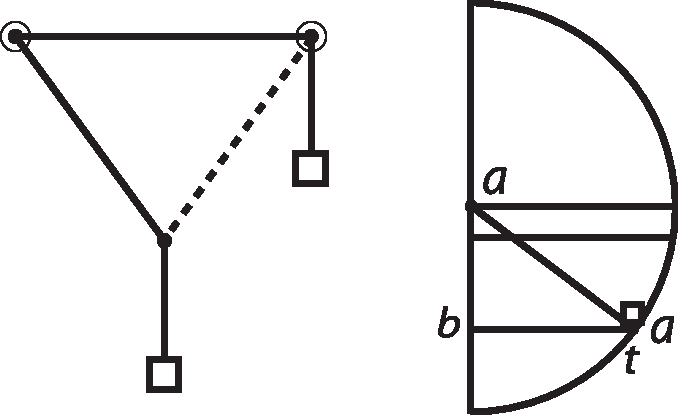
\includegraphics[trim = 0mm -5mm 0mm 0mm, clip, width=0.35\textwidth]{images//lh0351009_003r_2-d5+6.pdf}\\
\noindent \centering [\textit{Fig. 3 und Fig. 4 gestr.}]
%\end{wrapfigure}\\
%\includegraphics[width=0.2\textwidth]{images/lh0351009_003r_2-d5.pdf}
%\hspace{10mm} 
%\includegraphics[width=0.15\textwidth]{images/lh0351009_003r_2-d6.pdf}\\
%\vspace{8mm}
\pend
\vspace{2em}
\pstart
\noindent [\textit{Nachfolgend \setline{5}kleingedruckter Text gestrichen}:]
\pend
\vspace{0.5em}
\pstart
\noindent
\footnotesize
{Comme $b$ est \`{a} $a$, ainsi la force du poids\protect\index{Sachverzeichnis}{force du poids} descendant dans la} \edtext{\small{[circonference]}}{\lemma{}\Bfootnote{circomference \textit{L }\textit{\"{a}ndert Hrsg.}}} \small{du cercle, du point $ab$, est [\textit{Text bricht ab}.]} 
\pend
\count\Bfootins=1200
\count\Cfootins=1200

\vspace{12mm}
\section[\scriptsize\uppercase{R\`{e}gle pour calculer la force d'une machine. Premier essai, deuxi\`{e}me mouture}]{\uppercase{R\`{e}gle pour calculer la force d'une machine. Premier essai, deuxi\`{e}me mouture}}%
\addcontentsline{toc}{section}{\thesection\enskip R\`{e}gle pour calculer la force d'une machine. Troisi\`{e}me essai}
\vspace{4mm}
%    \begin{ledgroupsized}[r]{120mm}
\footnotesize 
\pstart    
\noindent\textbf{\"{U}berlieferung:} 
\pend
\end{ledgroupsized}
\begin{ledgroupsized}[r]{114mm}
\footnotesize 
\pstart \parindent -6mm
\makebox[6mm][l]{\textit{L}}%
Reinschrift mit Verbesserungen: LH XXXV 10, 9 Bl. 2. 1 Bl. beschnitten (11 x 17 cm). 1 S. auf Bl.~2~r\textsuperscript{o}. Bl.~2~v\textsuperscript{o}
leer. Auszug aus N. 28\textsubscript{1} mit Änderungen.\\
Cc 2, Nr. 1190 B
\pend
\end{ledgroupsized}

\vspace{8mm}
\pstart
\noindent
[2~r\textsuperscript{o}]
\pend
\pstart\noindent
\normalsize
Appellons \begin{tabular}[t]{lr}
le sinus droit \textit{EM},&\textit{y}\\
le Rayon \textit{AL},&\textit{a}\\
le petit Rayon \textit{LI} ou \textit{LK},&\textit{b}\\
la force absolue du poids,&\textit{g}\\
\end{tabular}
\pend
\vspace{0.5em}
\pstart \noindent et \setline{10}\textso{la force de la machine} sera $\rule[-4mm]{0mm}{10mm}\displaystyle\frac{yag + ag\sqrt{a^2 - y^2} - gby - gb\sqrt{a^2 - y^2}}{ba}$, ou $\rule[-4mm]{0mm}{10mm}\displaystyle y + \sqrt{a^2 - y^2}, \smallfrown \frac{a}{b} - 1, \smallfrown \frac{g}{a}$. C'est \`{a} dire, prenez la somme de \textit{ME} et \textit{ML}; et la multipliez par $\rule[-4mm]{0mm}{10mm}\displaystyle\frac{a}{b}-1$; et le produit, par $\rule[-4mm]{0mm}{10mm}\displaystyle\frac{g}{a}$. Ce qui en proviendra, sera la force de la machine\protect\index{Sachverzeichnis}{machine}, en quelque situation qu'elle puisse estre. Ou si vous voulez la force absolue du poids\protect\index{Sachverzeichnis}{poids}, sera \`{a} la force de la machine, dans l'estat donn\'{e}, comme $ba$ \`{a} $\rule[-4mm]{0mm}{10mm}\displaystyle y + \sqrt{a^2 - y^2}, \smallfrown a - b$ \textso{et en termes de Geometrie\protect\index{Sachverzeichnis}{geometrie}, comme le rectangle \textit{ELK}, au rectangle compris soubs }\edtext{\textso{\textit{HI} et \textit{MN}}}{\lemma{\textit{HI} et}\Bfootnote{\textit{(1)}\ $LM+ME$ \textit{(2)}\ \textit{MN}: \textit{L}}}: Theoreme\protect\index{Sachverzeichnis}{theoreme} assez beau, et d'un tres grand usage pour \edtext{calculer}{\lemma{}\Bfootnote{calculer \textit{erg. L}}} toutes sortes des mouuements circulaires\protect\index{Sachverzeichnis}{mouvement circulaire}.
\pend

\vspace{12mm}
\section[\scriptsize\uppercase{R\`{e}gle pour calculer la force d'une machine. Deuxi\`{e}me essai, deuxi\`{e}me mouture}]{\uppercase{R\`{e}gle pour calculer la force d'une machine. Deuxi\`{e}me essai, deuxi\`{e}me mouture}}%
\addcontentsline{toc}{section}{\thesection\enskip R\`{e}gle pour calculer la force d'une machine. Quatri\`{e}me essai}
\vspace{4mm}
%    \begin{ledgroupsized}[r]{120mm}
\footnotesize 
\pstart    
\noindent\textbf{\"{U}berlieferung:} 
\pend
\end{ledgroupsized}
\begin{ledgroupsized}[r]{114mm}
\footnotesize 
\pstart \parindent -6mm
\makebox[6mm][l]{\textit{L}}%
Reinschrift mit Verbesserungen: LH XXXV 10, 9 Bl. 1. 1 Bl. 4\textsuperscript{o}. 1 S. auf Bl.~1~r\textsuperscript{o}. Bl.~1~v\textsuperscript{o} leer. Unvollständige Abschrift von N. 28\textsubscript{2}.
\\ 
Cc 2, Nr. 1190 A
\pend
\end{ledgroupsized}
\count\Bfootins=1200
\vspace*{8mm}
%\pstart 
%\normalsize
%{\centering[1~r\textsuperscript{o}] Regle\\
%pour calculer la force\protect\index{Sachverzeichnis}{force} d'une\\
%Machine\protect\index{Sachverzeichnis}{machine}, dont voicy la figure\\}
\pstart 
\normalsize
\noindent
[1~r\textsuperscript{o}]
\pend
\pstart
\centering
\noindent
Regle pour calculer la force d'une Machine,\protect\index{Sachverzeichnis}{machine}\protect\index{Sachverzeichnis}{force}\\%
dont voicy la figure
\pend
\vspace{1.0em}
\pstart
\noindent
Soit la roue\protect\index{Sachverzeichnis}{roue} \textit{ABCD} mobile \`{a} l'entour du \edtext{centre \textit{L},}{\lemma{centre \textit{L}}\Bfootnote{\textit{(1)} . Supposons qu'elle est \textit{(2)} , entrecoup\'{e}e \textit{L}\hspace{-2mm}}} \edtext{entrecoup\'{e}e \`{a} angles \mbox{droits} de deux}{\lemma{}\Bfootnote{\`{a} angles droits \textit{erg. L}\hspace{-2mm}}} Diametres\protect\index{Sachverzeichnis}{diametre} solides \textit{AC}, et \textit{DB}; les quels seront transferez par le mouuement\protect\index{Sachverzeichnis}{mouvement} \`{a} l'entour du centre, de la situation perpendiculaire ou \edtext{horizontale, \mbox{\textit{ABCD}}, \`{a} l'inclin\'{e}e}{\lemma{}\Bfootnote{\textit{ABCD}, \textit{erg. L}}} \textit{EFGH} dans un \textso{angle donn\'{e}} \textit{ALE}. Conceuuons la dite roue charg\'{e}e dans les points, \textit{E}, \textit{F}, \textit{K}, \textit{I}, de quatre poids \'{e}gaux entre eux.
\pend
\vspace{1.5em}
\pstart
\centering
%\begin{wrapfigure}[17]{l}{0.5\textwidth}
%\vspace{-4mm}
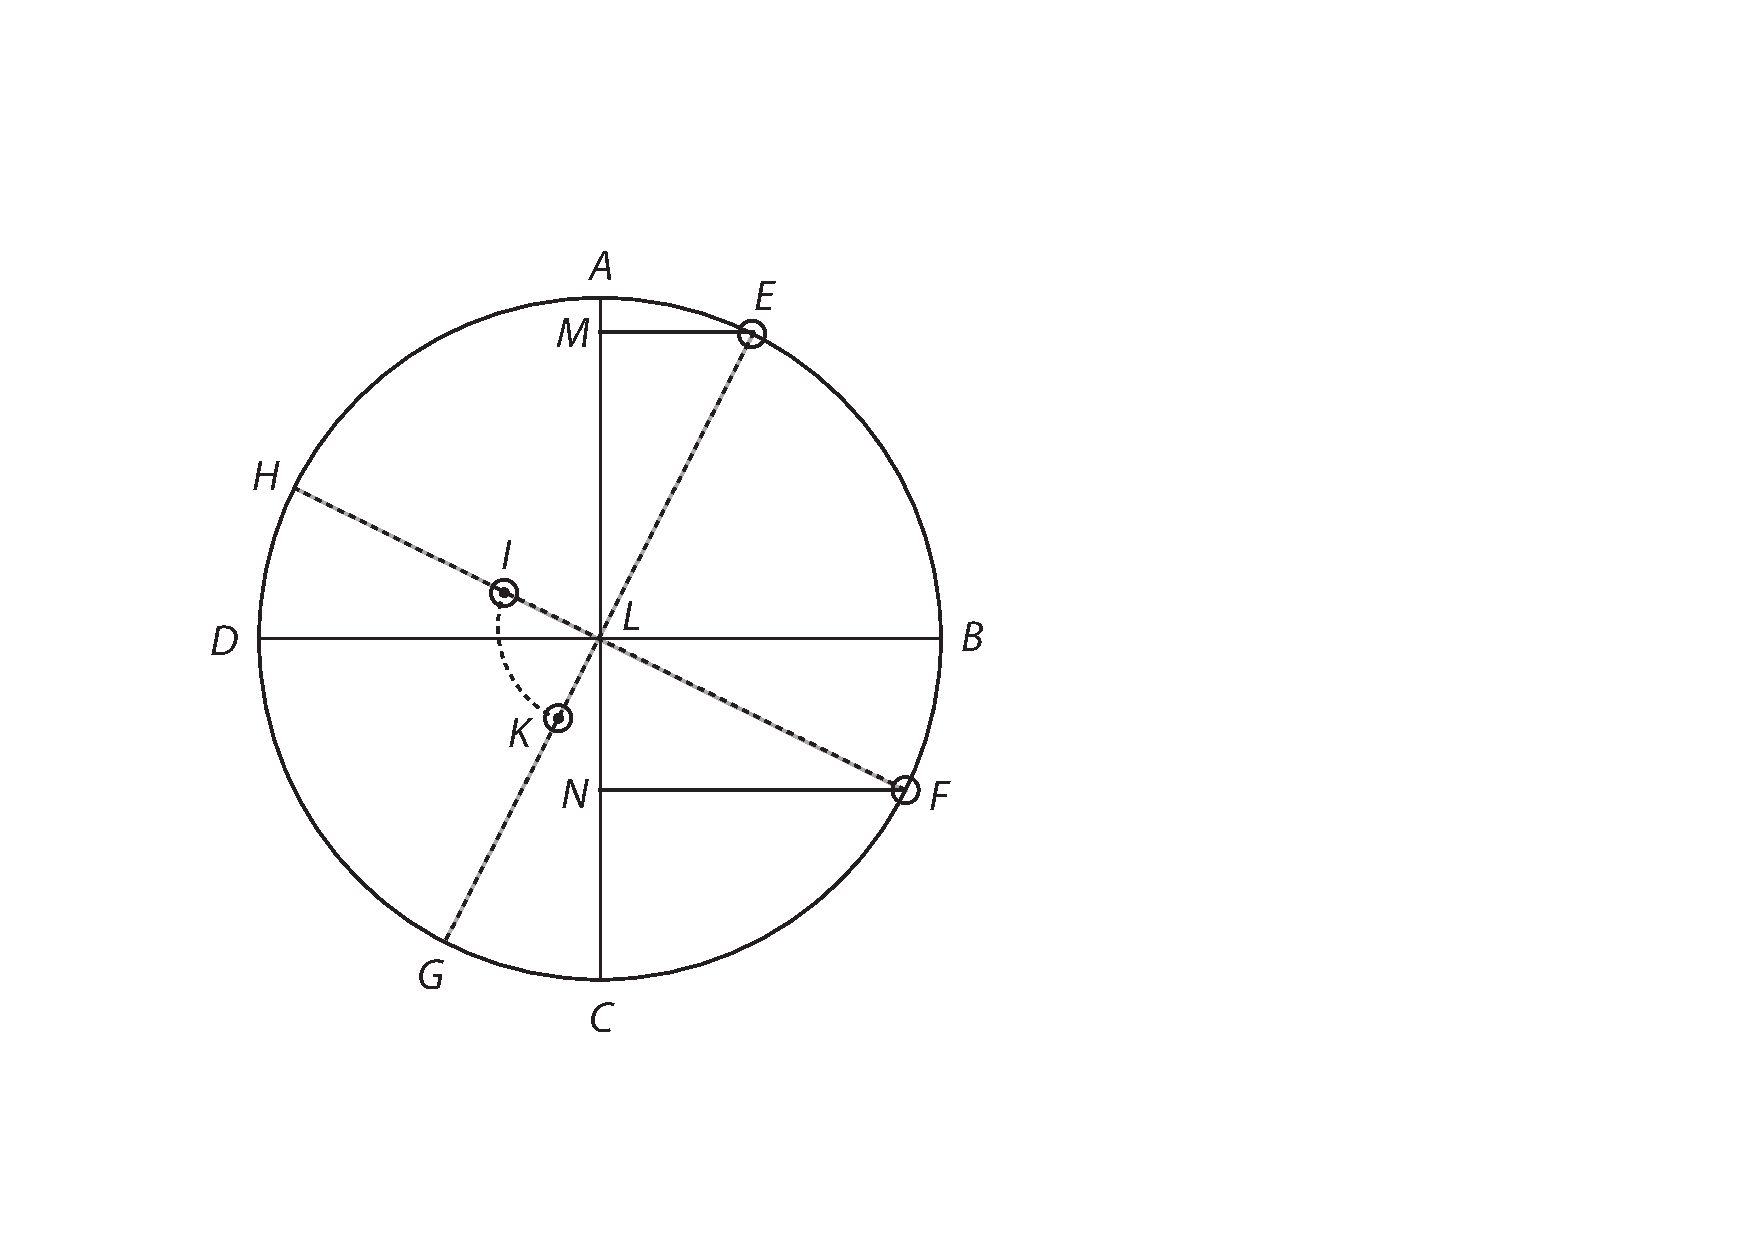
\includegraphics[trim = 0mm 0mm 0mm 0mm, clip, width=0.5\textwidth]{images/lh0351009_001r-d1.pdf}\\
\noindent \centering [\textit{Fig. 1}]
%\caption{Bildbeschreibung}
%\end{wrapfigure}
\pend
\newpage
\pstart
\indent Soit \textso{donn\'{e}e} la longueur de \textit{AC}, diametre\protect\index{Sachverzeichnis}{diametre} de la Roue, item la longueur des droites \textit{ELK}, ou \textit{FLI} \'{e}gales entre elles.\\
\indent Et enfin \textso{la force absolue}\protect\index{Sachverzeichnis}{force absolue} d'un de ces poids, c'est \`{a} dire avec la quelle il agit libr\`{e}ment, ou sur un plan parallele \`{a} l'horison, s'il en 
estoit soutenu.\\
\indent On demande la \edtext{force\protect\index{Sachverzeichnis}{force} de la machine\protect\index{Sachverzeichnis}{machine}, qu'elle auroit dans}{\lemma{force}\Bfootnote{\textit{(1)}\ absolue de la machine\protect\index{Sachverzeichnis}{machine}, dans \textit{(2)}\ de la machine\protect\index{Sachverzeichnis}{machine}, qu'elle auroit dans \textit{L}}} l'Estat \textit{EFGH}, si elle y commenceroit le mouuement\protect\index{Sachverzeichnis}{mouvement}; car il faut adjouter cette condition \`{a} fin de ne pas embarasser le calcul de la force simple\protect\index{Sachverzeichnis}{force simple}, par celuy de la force gagn\'{e}e\protect\index{Sachverzeichnis}{force gagn\'{e}e} 
par l'acceleration\protect\index{Sachverzeichnis}{acceleration}, \edtext{dont le calcul\protect\index{Sachverzeichnis}{calcul} se doit}{\lemma{dont}\Bfootnote{\textit{(1)}\ il faut \textit{(2)}\ le calcul se
doit \textit{ L}}} faire \`{a} part. 
\pend 
%\newpage
\pstart
Des points, \textit{E.F} menez les perpendiculaires \textit{EM}, \textit{FN}, sur le diametre\protect\index{Sachverzeichnis}{diametre} vertical \textit{AC}, les quelles seront \textso{donn\'{e}es}, par ce que les Angles \textit{ALE}, \textit{CLF} sont donn\'{e}s, dont elles sont les 
sinus droits. 
\pend 
\pstart
\textso{Cela estant pos\'{e}, je dis que la force absolue\protect\index{Sachverzeichnis}{force absolue} d'un des poids susdits est \`{a} la force\protect\index{Sachverzeichnis}{force} de la machine, comme le rect}\-\textso{angle \textit{ELK} (: ou compris soubs \textit{EL}, \textit{LK} :) est au rectangle compris soubs \textit{HI} et \textit{MN}.}\pend \pstart
Theoreme assez beau, et d'un tres grand usage pour le calcul des mouuements\protect\index{Sachverzeichnis}{mouvement} circulaires. \pend \pstart
Pour donner cette raison en nombres, il faut se servir des lettres de l'Analyse\protect\index{Sachverzeichnis}{analyse}, qui signifient des nombres indefinis, 
\pend 
\count\Bfootins=1500
\pstart
Soit
\begin{tabular}[t]{lr}
le sinus droit \textit{EM} appell\'{e},&\textit{y}\hspace{0.1mm}\\
le Rayon \textit{AL}&\textit{a}\\
le petit Rayon \textit{LI}&\textit{b}\\
\end{tabular}
\pend
\vspace{1mm}
\pstart\noindent
et\setline{23} la force absolue\protect\index{Sachverzeichnis}{force absolue} d'un des poids
sera \`{a} la force de la Machine\protect\index{Sachverzeichnis}{machine},
comme est 1, ou l'unit\'{e}, \`{a} $\rule[-4mm]{0mm}{12mm}\displaystyle\frac{y + \sqrt{a^2 - y^2}, \smallfrown a - b}{ba}$
ou comme 1,
\`{a} $\rule[-4mm]{0mm}{10mm}\displaystyle\frac{ya - yb + a\sqrt{a^2 - y^2} - b\sqrt{a^2 - y^2}}{ba}$. 
\pend

\vspace{12mm}
\section[\scriptsize\uppercase{De determinatione machinae virium per accelerationem acquisitarum}]{\uppercase{De determinatione machinae virium per accelerationem acquisitarum}}%
\addcontentsline{toc}{section}{\thesection\enskip De determinatione machinae virium per accelerationem acquisitarum}
\vspace{4mm}
%    \begin{ledgroupsized}[r]{120mm}
\footnotesize 
\pstart 
\noindent\textbf{\"{U}berlieferung:}
\pend
\end{ledgroupsized}
\begin{ledgroupsized}[r]{114mm}
\footnotesize 
\pstart \parindent -6mm
\makebox[6mm][l]{\textit{L}}%
Konzept: 
LH XXXV 10, 9 Bl. 3-4. 1 Bog. 2\textsuperscript{o}. 1\,\nicefrac{1}{2} S. auf Bl. 4.
Der Bogen überliefert ferner  N.~28\textsubscript{1}, N.~28\textsubscript{2}, N.~28\textsubscript{5} und N.~5.
%LH35,10,09 Bl. 3r = Demonstratio geometrica de magnetis sphaera
\\
Cc 2, Nr. 1192 A-B
\pend
\end{ledgroupsized}
%
%\vspace*{5mm}
%\begin{ledgroup}
%\footnotesize 
%\pstart
%\noindent\footnotesize{\textbf{Datierungsgr\"{u}nde}: nur chronologische Einordnung, Datierung nicht erfolgt}
%\pend
%\end{ledgroup}

\vspace*{8mm}
\pstart 
\normalsize
\noindent
[4~r\textsuperscript{o}] Determinata machinae vi\protect\index{Sachverzeichnis}{vis} per certam quandam relationem seu velut aequationem, ut hoc loco: \rule[-4mm]{0pt}{10mm}$\displaystyle\frac{ya + a \sqrt{a^2-y^2} - yb - b\sqrt{a^2-y^2}}{ba}$. 
\pend
\pstart
Hinc determinari potest vis\protect\index{Sachverzeichnis}{vis} ejus per accelerationem\protect\index{Sachverzeichnis}{acceleratio} acquisita. Nam regula generalis \makebox[1.0\textwidth][s]{est: sit figura $ABC$ cujus ordinatarum differentiae, $FG. HI. KB$, sint ut vires machinae\protect\index{Sachverzeichnis}{vires machinae}}
\pend
\vspace{1em}
\begin{minipage}[t]{0.5\textwidth}
%\hspace*{-5mm}
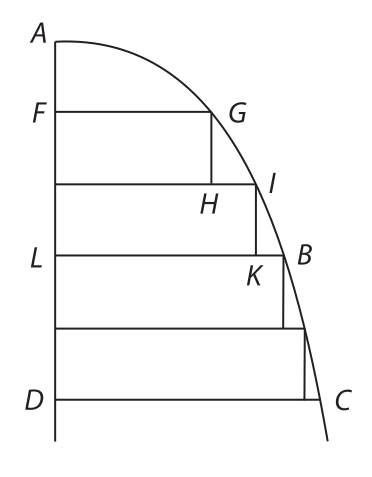
\includegraphics[width=0.65\textwidth]{images/lh0351009_004r-d1.pdf}
%\noindent \centering [\textit{Fig. 1}]
\end{minipage}
%\hspace*{17,3mm}
\begin{minipage}[t]{0.5\textwidth}
%\hspace*{-5mm}
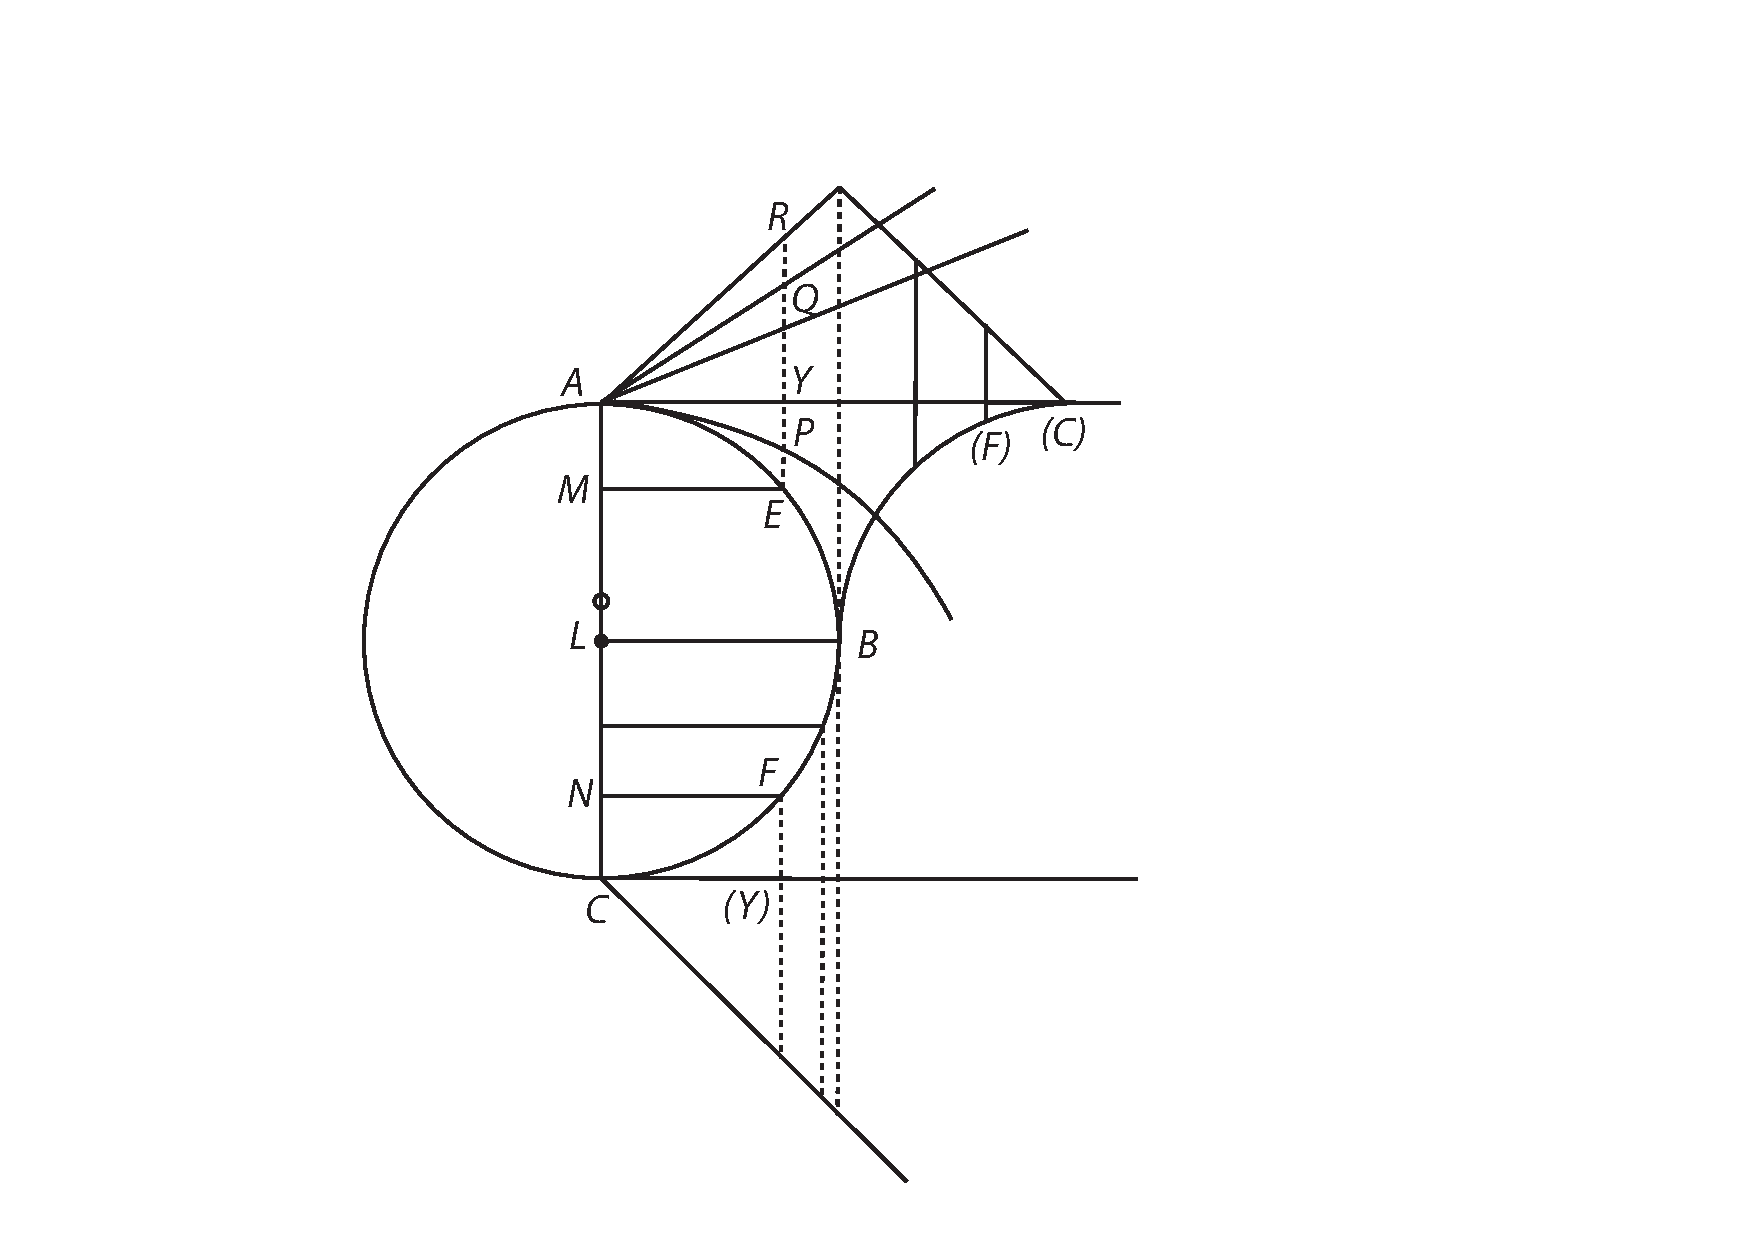
\includegraphics[width=1.0\textwidth]{images/lh0351009_004r-d2.pdf}
%\noindent \centering [\textit{Fig. 2}]
\end{minipage}
\vspace*{1em}
\hspace*{15mm} [\textit{Fig. 1}]\hspace*{70mm} [\textit{Fig. 2}]
\newpage
\count\Bfootins=1200
\pstart
 \noindent \edtext{simplices}{\lemma{}\Bfootnote{simplices \textit{erg. L}}} in quolibet loco; ordinatae erunt ut vires machinae\protect\index{Sachverzeichnis}{vires machinae} ex \edtext{acceleratione\protect\index{Sachverzeichnis}{acceleratio}, in}{\lemma{}\Bfootnote{acceleratione \textbar\ factae \textit{gestr.} \textbar\ , in \textit{L}}} quolibet loco, quippe harum differentiarum \edtext{summae. Aliter si sit figura}{\lemma{summae.}\Bfootnote{\textit{(1)} Aliter describatur figura omnium \textit{(2)} Aliter si sit figura \textit{L}}} cujus ordinatae sint ut $FG. HI. KB$ homogenea illis scilicet, cylinder\protect\index{Sachverzeichnis}{cylinder} ipsarum $LB$, exhibebit vires acceleratas\protect\index{Sachverzeichnis}{vis accelerata}, nempe rectangulum sub $LB$, et recta constante velut $A$. 
\pend
%\begin{figure}[t]
%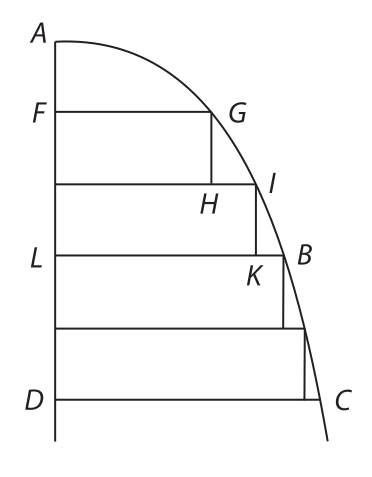
\includegraphics[width=0.2\textwidth]{images/lh0351009_004r-d1.pdf}\hspace{5mm}
%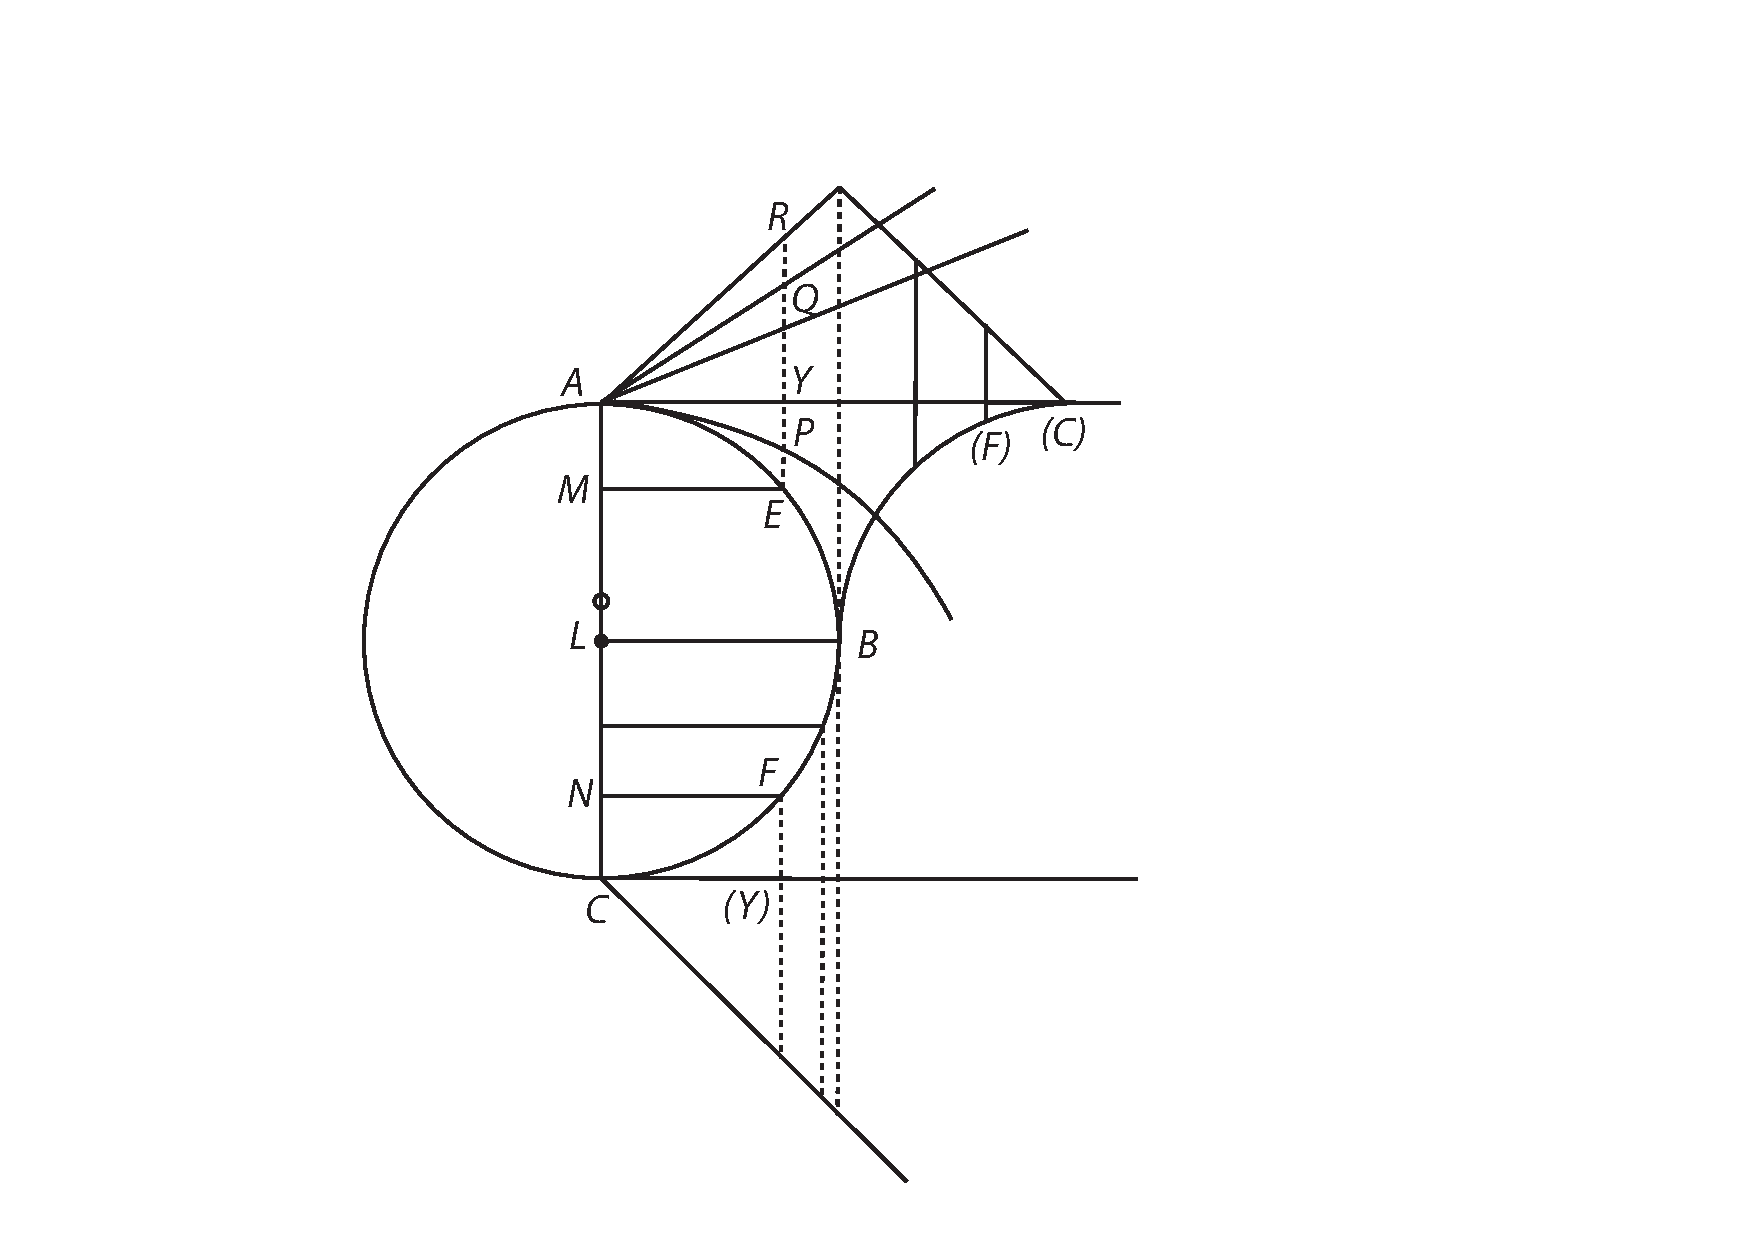
\includegraphics[width=0.4\textwidth]{images/lh0351009_004r-d2.pdf}\\
%\hspace{15mm} [\textit{Fig. 1}] \hspace{35mm} [\textit{Fig. 2}]
%\end{figure}
\pstart Centro $L$ ut ante sit idem circulus $AE$ in tangente verticis $A$, sume $AY$, quamlibet aequalem cuilibet $EM \hspace{0.1mm} \sqcap  \hspace{0.1mm}y$. Cui applicabis \edtext{$YR \hspace{0.1mm} \sqcap \hspace{0.1mm}y$}{\lemma{applicabis}\Bfootnote{\textit{(1)} $YR \sqcap \displaystyle\frac{a}{b}$ \textit{(2)} $ YR \sqcap y$ \textit{L}}} ab uno latere, quae sunt ad lineam rectam $AR$, et \edtext{$YE \sqcap AM \sqcap \sqrt{a^2-y^2}$}{\lemma{et}\Bfootnote{\textit{(1)} ${\displaystyle\frac{b \sqrt{a^2 - y^2}}{a}}$ \textit{(2)} $YE \sqcap AM \sqcap \sqrt{a^2-y^2}$ \textit{L}}} ab altero latere, quae sunt ad circumferentiam $AEB$, ab $AR$, aufer $RQ \sqcap \displaystyle\frac{yb}{a}$\rule[-4mm]{0pt}{10mm} quae sunt etiam ad lineam \edtext{rectam et ab $YE$}{\lemma{rectam}\Bfootnote{\textit{(1)} et $AR$ \textit{(2)} et ab $YE$ \textit{L}}} aufer $PE \sqcap b \sqrt{a^2-y^2}$ quae est ad Ellipsin, residua figura erit summa omnium virium seu quantitas \edtext{acceleratione\protect\index{Sachverzeichnis}{acceleratio} quaesita}{\lemma{acceleratione}\Bfootnote{\textit{(1)} genita \textit{(2)} quaesita \textit{L}}}. Porro pro $NF$, et aliis infra $LB$, eas applicabimus ad [$C(Y)$]\edtext{}{\Bfootnote{$CY$\textit{\ L \"{a}ndert Hrsg.}}}. Nisi malimus arcum $BFC$ illuc transferre in $B(F)(C)$, ut una inde fiat figura continua. His ergo intellectis breviter regulam ita concipiemus: 
\pend 
%\vspace{2mm}
\begin{center}                   
\noindent 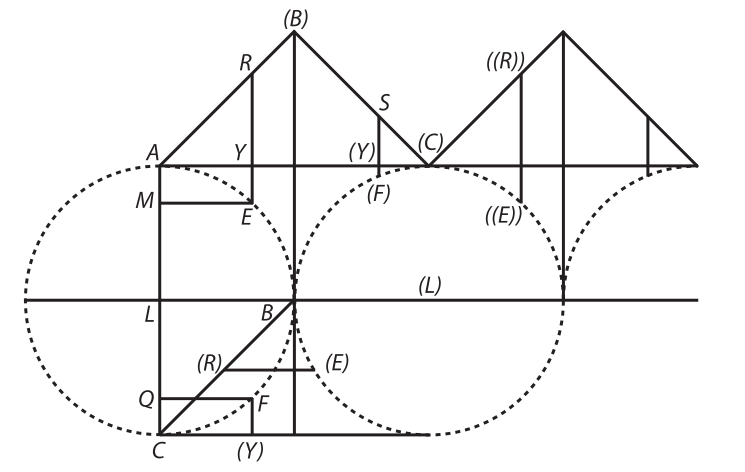
\includegraphics[width=0.86\textwidth]{images/lh0351009_004r-d3.pdf}\newline
[\textit{Fig. 3}]
\end{center}
\count\Bfootins=1200
\pstart Circuli $L\ AEBC$ rotam repraesentantis, verticem recta tangens $AY(C)$ producatur indefinite. Quemadmodum et diameter ejusdem horizonti parallela, $LB$ in qua sumta $(L)B \sqcap LB$ centro $L$, radio $LB$ describatur alius \edtext{circulus $(L)B(C)$}{\lemma{circulus}\Bfootnote{\textit{(1)} $L(B)C$ \textit{(2)} $(L)B(C)$ \textit{L}}} priori aequalis. Ex $B$ erigatur $B(B)$ ipsi $LB$ sive horizonti perpendicularis, et aequalis $AC$ circuli diametro, jungantur $A(B)$, $(B)(C)$. Et spatium \edtext{[$A(B)(C)(F)BE$]}{\lemma{}\Bfootnote{$A(B)(C)FBE$\textit{\ L \"{a}ndert Hrsg.}}} duobus circumferentiae quadrantibus $AEB$ et \textso{$B(F)(C)$} duabusque rectis \edtext{$A(B)$ et $(B)(C)$}{\lemma{}\Bfootnote{$A(B)$ et $(B)(C)$ \textit{erg. L}}} angulum comprehendentibus rectum, contentum erit accelerationibus\protect\index{Sachverzeichnis}{acceleratio} seu viribus crescentibus\protect\index{Sachverzeichnis}{vires crescentes} homogeneum. Nimirum pone motum incipere \edtext{in $E$, nempe $AC$ extremo diametri solidae in $E$, prius}{\lemma{incipere}\Bfootnote{\textit{(1)} $A$ in extremo diametri solidae in $E$, \textit{(2)} in $E$ nempe [...] $E$, prius \textit{L}}} translato, et quaeri quanta sit vis acquisita machinae in \edtext{quodam}{\lemma{}\Bfootnote{quodam \textit{erg. L}}} puncto, v.g. $F$, ad vim\protect\index{Sachverzeichnis}{vis} quaesitam in alio puncto \edtext{v.g. $B$. Ducatur recta $ER$ parallela ipsi $B(B)$, arcui pariter $AEB$, et rectae $A(B)$ occurrens. Inde in quadrante $B(C)$ sumto arcu $B(F)$ aequali}{\lemma{v.g. $B$.}\Bfootnote{\textit{(1)} Sume arcum \textit{(2)} Ducatur recta \textit{ER} parallela \textbar\ ipsi \textit{erg.} \textbar\ $B(B)$, [...] Inde \textit{(a)} sumto arcu $BF$ \textit{(b)} in quadrante [...] aequali \textit{L}}} arcui $BF$ ducatur eodem modo recta [$(F)S$]\edtext{}{\Bfootnote{$FS$\textit{\ L \"{a}ndert Hrsg.}}}, eritque vis acquisita in $F$ ad vim acquisitam\protect\index{Sachverzeichnis}{vis acquisita} in $B$, ut spatium $ER(B)BE$, ad spatium $ER(B)S(F)BE$. Unde apparet si nulla vi extrinseca\protect\index{Sachverzeichnis}{vis extrinseca} accedente repeti fingatur circulatio etiam figuram $A(B)(C)(F)BE$, repetendam, et si exempli causa repetita circulatione rursus pervenerit in $E$ vim acquisitam\protect\index{Sachverzeichnis}{vis acquisita} fore ut spatium $ER(B)(C)(F)BE + ((E))((R))(C)((E))$ id est si motus in $E$ incepisse intelligatur ut spatium $A(B)(C)(F)BE$. Nam si motus in $A$ coepisset, foret ut $A(B)(C)(F)BE + ((E))((R))(C)((E))$ quorum facilis ex superioribus demonstratio est nam si superiores vires simplices\protect\index{Sachverzeichnis}{vis simplex} dividantur per constantem quantitatem omnibus communem, \rule[-4mm]{0pt}{10mm}$\displaystyle \frac{a-b}{ba}$ restabit: $ y + \sqrt{a^2-y^2} \sqcap ER$ quia $ EY \sqcap AM \sqcap \sqrt{a^2-y^2}$ et $YR \sqcap AY \sqcap ME \sqcap y$ quod idem in aliis punctis omnibus obtinet.
\pend 
\pstart \edtext{Sed in machina praesente}{\lemma{Sed}\Bfootnote{\textit{(1)} id quidem \textit{(2)} in machina praesente \textit{L}}} figurae $\aleph$ motu semel in $A$, vel inter $A$ et $B$ coepto. Descensus infra $B$ aestimari non debet; nam inspecta dicta figura $\aleph$. $LE$ diametro rotae solido translato in $LB$ et $LH$ in $LA$ pondus $I$ transibit in $A$, et $LF$ eodem tempore in $C$ translato pondus $F$ assurget versus $L$, verbo redibit status primus $ABCD$.
\pend 
\count\Bfootins=1500
\pstart Pour estimer la force\protect\index{Sachverzeichnis}{force} de la m\^{e}me machine gagn\'{e}e par l'acceleration\protect\index{Sachverzeichnis}{acceleration}; du centre L, et du rayon $LA$ pris \`{a} discretion soit d\'{e}crit le quart de cercle, $LAEB$, le quel soit continu\'{e} mais d'une maniere renvers\'{e}e en forme de serpentine ou 
\includegraphics[width=0.035\textwidth]{images/lh0351009_004r-d6.pdf} (\includegraphics[width=0.035\textwidth]{images/lh0351009_004r-d7.pdf}) en $B(E)(B)$ et cette \makebox[1.0\textwidth][s]{continuation renvers\'{e}e sera repet\'{e}e autant de fois, que la roue de la Machine propos\'{e}e}
\pend
\begin{center}                    
\includegraphics[width=0.8\textwidth]{images/lh0351009_004r-d4.pdf}\\
\hspace{20mm}[\textit{Fig. 4}]
\end{center}
\count\Bfootins=1200
\pstart
\noindent achevera \setline{1}un quart de son tour. \edtext{Soit $BC$, double de $AL$ et parallele \`{a} la m\^{e}me men\'{e}e}{\lemma{Soit $BC$,}\Bfootnote{\textit{(1)} men\'{e}e parall\`{e}le \`{a} $AL$, dont elle soit le double \textit{(2)} double [...] men\'{e}e \textit{L}}} du cost\'{e} de $A$. Joignez $AC$ de m\^{e}me joignez $B(C)$ supposant $AL(C)$ et $(B)(C)$ egales entre elles et \`{a} $BC$. 
\pend
\pstart Or supposons que dans la fig. $\aleph$, le poids \edtext{superieur $E$ \`{a} main droite ou celuy qui luy succedera soit}{\lemma{}\Bfootnote{\`{a} main [...] succedera \textit{erg. L}}} dans le \edtext{point $E$ ou $P$ de la}{\lemma{point $E$}\Bfootnote{\textbar\ ou $P$ \textit{erg.} \textbar\ de la \textit{L}}} dite \edtext{figure $\aleph$ r\'{e}pondant au point $E$ ou $P$}{\lemma{figure $\aleph$}\Bfootnote{\textit{(1)} semblable ou proportionel \`{a} l'arc $AC$ \textit{(2)} r\'{e}pondant au point $E$ ou $P$ \textit{L}}} de la figure \edtext{presente, ou qu'il vienne dans la revolution ou repetition seconde, au}{\lemma{presente, ou}\Bfootnote{\textit{(1)} que dans la seconde \textit{(2)} qu'il \textit{(a)} soit \textit{(b)} vienne [...] seconde, \textit{(aa)} dans le \textit{(bb)} au \textit{L}}} poinct $(E)$ \edtext{de la figure $\aleph$}{\lemma{}\Bfootnote{de la figure $\aleph$ \textit{erg. L}}} qui repond au point $(E)$ de la figure presente. Du point $E$ ou $P$, ou $(E)$ soyent \edtext{[men\'{e}es]}{\lemma{}\Bfootnote{men\'{e}e \textit{L \"{a}ndert Hrsg.}}} sur $AC$, ou $B(C)$ les droites \edtext{ou ordonn\'{e}es}{\lemma{ou ordonn\'{e}es}\Bfootnote{\textit{erg. L}}} $ER$ ou $PS$, ou $(E)(R)$ paralleles \`{a} $BC$ ou $(B)(C)$. Et soit le \edtext{point $A$ ou $E$ celuy du}{\lemma{point}\Bfootnote{\textit{(1)} $E$ \textit{(2)} $A$ ou $E$ celuy du \textit{ L}}} commencement du mouuement\protect\index{Sachverzeichnis}{mouvement}, et celuy du \edtext{point $E$, ou $P$ ou $(E)$}{\lemma{point $E$,}\Bfootnote{\textbar\ ou \textit{erg.} \textbar\ $P$ ou $(E)$ \textit{L}}} celuy de la fin \edtext{dans le temps que nous le considerons}{\lemma{}\Bfootnote{dans [...] considerons \textit{erg. L}}}, je dis que les forces acquises\protect\index{Sachverzeichnis}{force acquise} sur la fin d'un chacun, seront entre elles comme les espaces compris entre les paralleles \edtext{ou ordonn\'{e}es}{\lemma{}\Bfootnote{ou ordonn\'{e}es \textit{erg. L}}} des points du commencement et de la fin. Par exemple si le mouuement\protect\index{Sachverzeichnis}{mouvement} a commenc\'{e} en $A$, la force de la machine\protect\index{Sachverzeichnis}{force de la machine}, acquise par l'acceleration\protect\index{Sachverzeichnis}{acceleration} pendant le poids superieur est en $E$, est \`{a} celle qui est \`{a} acquerir quand il sera en $P$, comme \edtext{l'espace}{\lemma{comme}\Bfootnote{\textit{(1)} les espaces \textit{(2)} l'espace \textit{L}}} $AREA$ compris entre \edtext{le point}{\lemma{}\Bfootnote{le point \textit{erg. L}}} $A$ ou ordonn\'{e}e du commencement infiniment petite, et $ER$ ordonn\'{e}e de la fin; \`{a} l'espace $ASPA$, compris entre $A$ et $PS$. De m\^{e}me la force\protect\index{Sachverzeichnis}{force gagn\'{e}e} gagn\'{e}e par le mouuement commenc\'{e} en $A$ et termin\'{e} en $E$, sera \`{a} la force gagn\'{e}e\protect\index{Sachverzeichnis}{force gagn\'{e}e} par le mouuement commenc\'{e} en $E$, et termin\'{e} en $P$, comme l'espace $AREA$ \`{a} l'espace $ERSPE$. Enfin la force \edtext{gagn\'{e}e\protect\index{Sachverzeichnis}{force gagn\'{e}e} dans}{\lemma{gagn\'{e}e}\Bfootnote{\textit{(1)} par \textit{(1)} dans \textit{L}}} une revolution \edtext{qui se fait pendant que le poids $E$ acheve le quart de cercle}{\lemma{revolution}\Bfootnote{ \textit{ (1) } (c'est \`{a} dire dans un tour du quart de cercle \textit{ (2) } qui [...] cercle \textit{ L}}} $AB$, sera \`{a} la force gagn\'{e}e\protect\index{Sachverzeichnis}{force gagn\'{e}e} dans une revolution et quelque chose d'avantage quand le poids superieur \`{a} main droite est \edtext{en $(E)$ sera comme}{\lemma{en $(E)$}\Bfootnote{\textit{(1)} sera \textit{(2)} comme \textit{L}}} l'espace $ACBA$, compris entre $A$ et $BC$, \`{a} l'espace [$ACBA + B(R)(E)B$]\edtext{}{\Bfootnote{$ACBA + BR(E)B$ \textit{L \"{a}ndert Hrsg.}}} compris entre l'ordonn\'{e}e du \edtext{commencement, s\c{c}avoir le point $A$ (dans cet exemple) et l'ordonn\'{e}e [$(E)(R)$] du}{\lemma{commencement,}\Bfootnote{\textit{(1)} s\c{c}avoir en cet \textit{(2)} s\c{c}avoir [...] \textbar\ $(E)R$ \textit{\"{a}ndert Hrsg.} \textbar\ du \textit{L}}} point de la fin $(E)$. 
\pend 
\count\Bfootins=1000
\pstart Il s'ensuit par l\`{a} que la vistesse croistra \`{a} l'infini, supposant le mouuement continuel, et faisant abstraction des obstacles qui peuuent se rencontrer dans le \edtext{medium; qui est l'air, et l'essieu\protect\index{Sachverzeichnis}{essieu}}{\lemma{medium;}\Bfootnote{\textit{(1)} et dans le poi \textit{(2)} qui est l'air, et l'essieu\protect\index{Sachverzeichnis}{essieu} \textit{L}}} \`{a} l'entour du quel tourne la roue. Car la vitesse\protect\index{Sachverzeichnis}{vitesse} pourroit devenir si grande, que ny l'essieu\protect\index{Sachverzeichnis}{essieu} ny l'air souffriroient l'un un glissement, l'autre une division si subite. Effectivement, si la machine se peut executer, elle viendra bien tost \`{a} une \edtext{vitesse\protect\index{Sachverzeichnis}{vitesse} tres considerable}{\lemma{vitesse}\Bfootnote{\textit{(1)} si grande \textit{(2)} tres considerable \textit{L}}}. Mais \edtext{il faut tacher}{\lemma{il}\Bfootnote{\textit{(1)} faut prendre garde \textit{(2)} faut tacher \textit{L}}} de faire en sorte \edtext{qu'elle devienne}{\lemma{qu'elle}\Bfootnote{\textit{(1)} puisse \textit{(2)} devienne \textit{L}}} jamais plus grande que celle avec la quelle l'aimant attire l'aiguille\protect\index{Sachverzeichnis}{aiguille}. C'est \`{a} dire qu'elle n'acheve pas le quart de cercle avant que l'aimant puisse retirer l'aiguille\protect\index{Sachverzeichnis}{aiguille}. Car cela \edtext{feroit cesser le mouuement en certains cas}{\lemma{feroit}\Bfootnote{\textit{(1)} culbuter la machine. C'est \`{a} dire cela la pourroit mettre en estat de cesser en certains cas \textit{(2)} cesser \textit{(a)} la ma \textit{(b)} le mouuement en certains cas. \textit{L}}}.
\pend
\count\Bfootins=1000
\pstart Il est vray que pendant que l'aiguille\protect\index{Sachverzeichnis}{aiguille} passe sans estre attir\'{e}e, l'acceleration\protect\index{Sachverzeichnis}{acceleration} seroit en m\^{e}me \edtext{temps decroissante}{\lemma{temps}\Bfootnote{\textit{(1)} croissante \textit{(2)} decroissante \textit{L}}}; le mouuement n'estant continu\'{e} par la force gagn\'{e}e\protect\index{Sachverzeichnis}{force gagn\'{e}e}, la quelle, n'estant plus suivie, se perdroit \edtext{peu \`{a} peu}{\lemma{}\Bfootnote{peu \`{a} peu \textit{erg. L}}} par l'obstacle du poids de l'aiguille\protect\index{Sachverzeichnis}{aiguille} \'{e}loign\'{e}e du centre plus qu'il ne faut; \edtext{ce qui peut estre matiere d'un calcul tres subtil}{\lemma{}\Bfootnote{ce qui [...] subtil. \textit{erg. L}}}. Mais l'acceleration\protect\index{Sachverzeichnis}{acceleration} de la force gagn\'{e}e\protect\index{Sachverzeichnis}{force gagn\'{e}e} pourroit estre si grande qu'elle ne donneroit point le loisir \`{a} la machine de se reconnoistre; et qu'elle emporteroit le canal de verre de l'aiguille\protect\index{Sachverzeichnis}{aiguille} qui deuuoit estre \edtext{[attir\'{e}e]}{\lemma{}\Bfootnote{attireroit\textit{\ L \"{a}ndert Hrsg.}}}, et le feroit passer jusque en haut, ou jusque en bas; o\`{u} les aiguilles\protect\index{Sachverzeichnis}{aiguille} demeureroient sans estre attir\'{e}es; et la machine demeureroit en repos; \`{a} moins que la force gagn\'{e}e\protect\index{Sachverzeichnis}{force gagn\'{e}e} fut capable toute seule de porter la machine jusqu' au deuxiesme tour de \edtext{roue dont le mouuement soit assez}{\lemma{roue}\Bfootnote{\textit{(1)} de la vistesse fut asse \textit{(2)} dont le mouuement \textit{(a)} fut \textit{(b)} soit assez \textit{L}}} doux \edtext{pour}{\lemma{}\Bfootnote{pour \textit{erg.} \textit{L}}} attendre l'action de l'aimant. 
\pend 
\vspace{-1mm}
\pstart
\begin{window}[0,r,\hspace{1mm}\includegraphics[%trim = -3mm -2mm 0mm 0mm, clip,
width=0.2\textwidth]
{images/lh0351009_004r-d5.pdf}, \hspace{7mm}{[\textit{Fig. 5}]}]
\indent
\edtext{Sed video jam me errasse, nam pro sinubus complementi $\sqrt{a^2-y^2}$ ut $LM$ applicavi sinus versos ut $AM$. Itaque $ER$ esse debebit, qualem in hac novissima figura vides. Succurrunt praeterea difficultates ingentes}{\lemma{7-10\hspace{1.8mm}}\killnumber\Bfootnote{Sed \textbar\ occurrunt \textit{streicht Hrsg.} \textbar\ \textit{(1)} hic duae difficultates ingentes, una an non potius sinus recti et ver \textit{(2)} video [...] $ \sqrt{a^2-y^2}$ \textbar\ ut $LM$ \textit{erg.} \textbar\ applicavi [...] ingentes \textit{L}}}. {Quarum\reversemarginpar\marginnote{\scriptsize\hspace{-13mm}10}} prima est an non ipsae $ER$ potius arcui $AEB$, sive in rectam extenso applicari in plano, sive manenti qualis est in superficie cylindrica insistere debeant. Idque rationi consentaneum magis, quia mobile percurrit curvam circularem $AEB$, et in quolibet arcu summam habet virium\protect\index{Sachverzeichnis}{vis} praecedentium omnium. Suppone autem arcum {divisum\reversemarginpar\marginnote{\scriptsize\hspace{-13mm}15}} in partes infinite parvas inter se aequales. Sed jam hanc quoque methodum [4~v\textsuperscript{o}] habeo suspectam \edtext{falsitatis. Equidem}{\lemma{16 \hspace{1.8mm}falsitatis.}\killnumber\Bfootnote{\textit{(1)} Nam \textit{(2)} Equidem \textit{L}}} supponendo\hspace{0.2mm} infinitos\hspace{0.3mm} istos\hspace{0.3mm} arcus\hspace{0.2mm} lineis\hspace{0.3mm} rectis\hspace{0.3mm} aequales.\hspace{0.3mm} Sit \hspace{0.2mm}\edtext{centro \textit{H}}{\lemma{17\hspace{1.8mm}}\killnumber\Bfootnote{centro \textit{H} \textit{erg. L}}}
\end{window}
%\begin{wrapfigure}[12]{l}{0.2\textwidth}                    
%\includegraphics[trim = 0mm -3mm -5mm 0mm, clip, width=0.2\textwidth]{images/lh0351009_004r-d5.pdf}\newline
%\noindent \centering [\textit{Fig. 5}]
%\end{wrapfigure}
%\edtext{Sed video jam me errasse, nam pro sinubus complementi $\sqrt{a^2-y^2}$ ut $LM$ applicavi sinus versos ut $AM$. Itaque $ER$ esse debebit, qualem in hac novissima figura vides. Succurrunt praeterea difficultates ingentes}{\lemma{}\Bfootnote{Sed \textbar\ occurrunt \textit{streicht Hrsg.} \textbar\ \textit{(1)} hic duae difficultates ingentes, una an non potius sinus recti et ver \textit{(2)} video [...] $ \sqrt{a^2-y^2}$ \textbar\ ut $LM$ \textit{erg.} \textbar\ applicavi [...] ingentes \textit{L}}}. Quarum prima est an non ipsae $ER$ potius arcui $AEB$, sive in rectam extenso applicari in plano, sive manenti qualis est in superficie cylindrica insistere debeant. Idque rationi consentaneum magis, quia mobile percurrit curvam circularem $AEB$, et in quolibet arcu summam habet virium\protect\index{Sachverzeichnis}{vis} praecedentium omnium. Suppone autem arcum divisum in partes infinite parvas inter se aequales. Sed jam hanc quoque methodum
%    %\hspace{-1.3mm}[4~v\textsuperscript{o}] habeo suspectam \edtext{falsitatis. Equidem}{\lemma{falsitatis.}\Bfootnote{\textit{(1)} Nam \textit{(2)} Equidem \textit{L}}} supponendo infinitos istos arcus lineis rectis aequales. 
%Sit \edtext{centro H}{\lemma{}\Bfootnote{centro H \textit{erg. L}}} circulus $ABC$ in cujus puncto $E$, sit tangens infinite parva $DE$, et ipsi $AC$ parallela
\noindent  circulus \setline{18}$ABC$ in cujus puncto $E$, sit tangens infinite parva $DE$, et ipsi $AC$ parallela $DF$ ad quam perpendicularis $EF$, et $BG$ \edtext{sinus anguli}{\lemma{}\Bfootnote{sinus \textbar\ versus \textit{gestr.} \textbar\ anguli \textit{L}\hspace{-3mm}}} $AHB$ erunt Triangula $DFE$ et $BGH$ similia adeoque [$DE$]\edtext{}{\Bfootnote{$BE$\textit{\ L \"{a}ndert Hrsg.}\hspace{-3mm}}}, ad $DF$ ut $BH$ ad $BG$. Jam \edtext{tempus ponderis\protect\index{Sachverzeichnis}{pondus} descendentis per $DE$ est aequale tempori}{\lemma{Jam}\Bfootnote{\textit{(1)} celeritas ponderis\protect\index{Sachverzeichnis}{celeritas ponderis} descendentis per $DE$ est \textit{(a)} ad celeritatem \textit{(b)} aequalis celeritati \textit{(2)} tempus [...] tempori \textit{L}\hspace{-3mm}}} ponderis descendentis per $DF$. Spatia autem inaequalia sunt. Ergo \edtext{celeritates\protect\index{Sachverzeichnis}{celeritas} erunt ut spatia percursa\protect\index{Sachverzeichnis}{spatia percursa} reciproce, ergo et vires\protect\index{Sachverzeichnis}{vis}}{\lemma{Ergo}\Bfootnote{\textit{(1)} vires erunt ut spatia \textit{(2)} celeritates [...] vires \textit{L}}}, \edtext{igitur}{\lemma{}\Bfootnote{igitur \textit{erg. L}\hspace{-3mm}}} vis\protect\index{Sachverzeichnis}{vis ponderis} ponderis in circumferentiae circuli puncto $B$, descensum molientis est ad \edtext{vim\protect\index{Sachverzeichnis}{vis} ejusdem [librae] descendentis in}{\lemma{vim}\Bfootnote{\textit{(1)} corporis in \textit{(2)} ejusdem \textbar\ liberi \textit{\"{a}ndert Hrsg.} \textbar\ descendentis in \textit{L}\hspace{-3mm}}} perpendiculari $DF$, ut $DF$ ad $DE$, \edtext{seu ut sinus rectus $BG$ ad radium $BH$}{\lemma{seu ut}\Bfootnote{\textit{(1)} radius $BH$, ad sinum rectum $BG$ \textit{(2)} sinus [...] $BH$ \textit{L}\hspace{-3mm}}}. Eodem modo vis\protect\index{Sachverzeichnis}{vis ponderis} ponderis in \edtext{[$NQ$]}{\lemma{$LD$}\Bfootnote{\textit{L \"{a}ndert Hrsg.}}}
ad vim ponderis in
\edtext{[$LD$]}{\lemma{$NQ$}\Bfootnote{\textit{L \"{a}ndert Hrsg.}}} est ut $PM$ \edtext{ad radium}{\lemma{ad}\Bfootnote{\textit{(1)} sinum \textit{(2)} radium \textit{L}}} $HM$.
\pend 
\pstart
\count\Bfootins=1500
\noindent
\centering
\includegraphics[width=0.65\textwidth]{images/lh0351009_004v-d1.pdf}\\
\centering [\textit{Fig. 6}]
\pend
\pstart \vspace{1em}Jam \setline{1}ponamus pondus descendisse per $LD$, \edtext{quae cum sit infinite parva nullam in ea considerabimus accelerationem\protect\index{Sachverzeichnis}{acceleratio}.}{\lemma{$LD$,}\Bfootnote{\textit{(1)} ducenda erit vis\protect\index{Sachverzeichnis}{vis} \textit{(2)} vis est \textit{(3)} sine acceleratione, ducenda est \textit{(4)} quae [...] accelerationem\protect\index{Sachverzeichnis}{acceleratio}. \textit{L}}} Ponendo radium 1 vis descendentis in $LD$ \edtext{erit $\sqcap \hspace{0.6mm}PM$}{\lemma{erit}\Bfootnote{\textit{(1)} $y\hspace{0.6mm} \sqcap$ \textit{(2)} $\sqcap \hspace{0.6mm}PM$. \textit{L}}}. 
\pend 
\pstart Pone corpus aliquod grave descendere in recta $AF$, ac primum percurrere $AB$ spatium minus quovis dato, \edtext{in tempore minore quovis dato $BC$}{\lemma{dato,}\Bfootnote{\textit{(1)} $\sqcap$ \textit{(2)} in [...] dato $BC$ \textit{L}}} spatium $BD$ \edtext{in tempore $DE$}{\lemma{$BD$}\Bfootnote{\textit{(1)} absolvet \textit{(2)} in tempore $DE$, \textit{L}}}, et spatium $DF$ in tempore \edtext{$FG$, erit tempus}{\lemma{$FG$,}\Bfootnote{\textit{(1)} erunt spatia in \textit{(2)} erit tempus \textit{L}}} quo percurritur spatium $AD$, ad tempus quo percurritur spatium $AF$, ut $ADE$ ad $AFG$, seu in duplicata spatiorum ratione.
Itaque \edtext{si grave per spatium pedis unius}{\lemma{si}\Bfootnote{\textit{(1)} mobile spatium 1 \textit{(2)} grave per spatium pedis unius \textit{L}}} descendet scrupulo secundo unico, descendet per spatium duorum scrupulis secundis quatuor, atque ita retardabitur motus. Jam contra fingamus $AB$ esse vel $AD$ vel $AF$ esse tempus et $BC$, $DE$, $FG$ esse spatium; erunt spatia percursa in duplicata temporum ratione, et per consequens; ita motus accelerabitur. Tempus ergo
\pend
\pstart
%\vspace{1ex}
\noindent
\begin{minipage}[t]{0.5\textwidth}
\hspace*{15mm}
\includegraphics[width=0.75\textwidth]{images/lh0351009_004v-d2.pdf}
%\noindent \centering [\textit{Fig. 7}]
\end{minipage}
\hspace*{25mm}
\begin{minipage}[t]{0.5\textwidth}
%\hspace*{-5mm}
\includegraphics[width=0.45\textwidth]{images/lh0351009_004v-d2a.pdf}
%\noindent \centering [\textit{Fig. 8}]
\end{minipage}\\
\vspace{8mm}
\hspace*{32mm} [\textit{Fig. 7}] \hspace*{55mm}  [\textit{Fig. 8}]
\pend
%\vspace{0.5em}
\vspace{1.5em}
\pstart
\noindent
\begin{minipage}[t]{0.5\textwidth}
\hspace*{23mm}                    
\includegraphics[width=0.45\textwidth]{images/lh0351009_004v-d3.pdf}
\end{minipage}
\hspace*{25mm}
\begin{minipage}[t]{0.5\textwidth}
\includegraphics[width=0.45\textwidth]{images/lh0351009_004v-d4.pdf}
% [\textit{Fig. 9}] \hspace{15mm} [\textit{Fig. 10}]
\end{minipage}\\
\vspace{8mm}
\hspace*{32mm} [\textit{Fig. 9}] \hspace*{55mm}  [\textit{Fig. 10}]\setline{1}
\pend
\vspace{2.5em}
\pstart \noindent considerandum \setline{1}est velut partes axis; vis simplex\protect\index{Sachverzeichnis}{vis simplex} in quolibet momento temporis exercita velut differentiae ordinatarum; vis acquisita\protect\index{Sachverzeichnis}{vis acquisita} in quolibet momento temporis, velut ordinatae; vires\protect\index{Sachverzeichnis}{vis} inter se ut ordinatae figurae: spatia percursa ut \edtext{portiones figurae}{\lemma{ut}\Bfootnote{\textit{(1)} spatia \textit{(2)} portiones figurae \textit{L}}}. Figura autem est semper Quadratrix \edtext{figurae differentiarum}{\lemma{Quadratrix}\Bfootnote{\textit{(1)} ordinatarum \textit{(2)} figurae differentiarum \textit{L}}} seu virium simplicium\protect\index{Sachverzeichnis}{vis simplex}.
\pend 
\vspace{2mm}
\count\Afootins=1250
\count\Cfootins=1250
%\newpage
\pstart \noindent$y + \sqrt{a^2 - y^2} \sqcap x.$ maximo. \\
\rule[-4mm]{0mm}{10mm}$ a^2 \raisebox{-3.2mm}{{\def\firstcircle{(0,0) circle (0.4cm)}\begin{tikzpicture}\draw \firstcircle node {$-y^2$};\end{tikzpicture}}} \sqcap x^2 - 2yx \raisebox{-3.2mm}{{\def\firstcircle{(0,0) circle (0.4cm)}\begin{tikzpicture}\draw \firstcircle node {$+y^2$};\end{tikzpicture}}}$\\
\rule[0pt]{26mm}{0pt} $+2y^2$\\
$-x^2 + 2yx \cdot \cdot\ + 2y^2 - 2yx$\\
$-\cancel{2}x^2 + \cancel{2}yx \sqcap + \overset{2}{\cancel4}yl - \cancel{2}lx$\\
\rule[-4mm]{0pt}{10mm}$l \sqcap \displaystyle\frac{-2x^2 + 2yx}{+2y - x}$\edtext{}{\lemma{$l \sqcap \displaystyle\frac{-2x^2 + 2yx}{+2y - x}$}\Cfootnote{Die Division durch 2 wurde nur im Nenner berücksichtigt. Der Fehler wirkt sich auf die weitere Ableitung aus.}}\\
\rule[-4mm]{0pt}{10mm}$x^2 \sqcap \raisebox{-3.2mm}{{\def\firstcircle{(0,0) circle (0.4cm)}\begin{tikzpicture}\draw \firstcircle node {$y^2$};\end{tikzpicture}}} + 2\sqrt{a^2 - y^2} + a^2 \raisebox{-3.2mm}{{\def\firstcircle{(0,0) circle (0.4cm)}\begin{tikzpicture}\draw \firstcircle node {$-y^2$};\end{tikzpicture}}}$\edtext{}{\lemma{$2\sqrt{a^2-y^2}$}\Cfootnote{Der Term lautet eigentlich
 $2y\sqrt{a^2-y^2}$. Der Fehler wirkt sich auf die weitere Ableitung aus.}}\\
\rule[-4mm]{0pt}{10mm}$l \sqcap \displaystyle\frac{-4\sqrt{a^2 - y^2} - 2a^2 + 2y^2 + 2y\sqrt{a^2 - y^2}}{\raisebox{-3.2mm}{{\def\firstcircle{(0,0) circle (0.4cm)}\begin{tikzpicture}\draw \firstcircle node {$2$};\end{tikzpicture}}} \ y \ \raisebox{-3.2mm}{{\def\firstcircle{(0,0) circle (0.4cm)}\begin{tikzpicture}\draw \firstcircle node {$-y$};\end{tikzpicture}}} - \sqrt{a^2 - y^2}}$\edtext{}{\lemma{$-4\sqrt{a^2 - y^2} - 2a^2 + 2y^2 + 2y\sqrt{a^2 - y^2}$}\Cfootnote{Der Z\"{a}hler lautet eigentlich
 $-2y\sqrt{a^2 - y^2} - a^2 + y^2 + y\sqrt{a^2 - y^2}$.}}\\
\rule[-4mm]{0pt}{10mm}$y \sqcap \sqrt{a^2 - y^2}$\hspace{3mm} $y^2 \sqcap a^2 - y^2$. Ergo $2y^2 \sqcap a^2$. Ergo $y \sqcap \displaystyle\frac{\PsMs\hspace{0.4mm} a}{\sqrt 2} \quad\displaystyle\frac{a}{1\displaystyle\frac{2}{5}} \quad \begin{array}{cc}a\\
\hline\hline \displaystyle\frac{7}{5} \end{array} \quad\displaystyle\frac{5a}{7}.$\edtext{}{\lemma{}\Afootnote{\textit{Nebenrechnungen}:\\ $\displaystyle\frac{200}{100}$ \hspace{3mm} $\displaystyle\frac{\displaystyle\efrac{\cancel{1}\cancel{2} 4}{\text{\d{$\cancel{\bullet}$}}\cancel{\bullet}\text{\d{$\cancel{\bullet}$}}}}{\displaystyle\frac{1\,\,\,4}{\cancel{1}\cancel{2}\cancel{4}}}$ \hspace{3mm} $\displaystyle\frac{14}{10} \bigg\vert \displaystyle\frac{7}{5} \sqcap 1 \displaystyle\frac{2}{5}$\vspace{-4mm}}}\\
$2y \sqcap x. \quad 2y \sqcap y + \sqrt{a^2 - y^2},$ ou $y \sqcap \sqrt{a^2 - y^2}$ ou $y^2 \sqcap a^2 - y^2$ ou $2y^2 \sqcap a^2.$ \edlabel{vismach1}
\edtext{}{{\xxref{vismach1}{vismach2}}\lemma{$y \hspace{0.3mm}\sqcap \displaystyle\frac{a}{\sqrt2}$}\Bfootnote{\textit{(1)} $z + \sqrt{2az - z^2}\hspace{0.4mm} \sqcap \hspace{0.4mm}\omega$ \hspace{1mm}  $\omega^2 - 2 \omega z + \cancel{2}z^2 \hspace{0.4mm}\sqcap \hspace{0.4mm}2az \protect\ovalbox{$-z^2$}$.\hspace{0.2mm} $\protect\begin{array}{ll}\cancel{2}\omega^2 - \cancel{2}\omega z + \cdots \sqcap - \protect\overset{2}{\cancel4}z^{\protect\textcircled{$\scriptstyle 2$}}\lambda &+\cancel{2}\omega \protect\textcircled{z} \lambda.\\ &+\cancel{2}a \,\,\cdot \;\;\cdot\protect\end{array}$ 
$\protect\begin{array}{rl}\hspace{-1.8mm}\lambda \sqcap \displaystyle\frac{\omega^2 - \omega z}{-2z + \omega} & \protect\atop{}{\displaystyle{2z \sqcap \omega + a. \quad z \sqcap \omega + a.}}\\ +a & \ \ z\sqcap z - \protect\end{array}$ \textit{ (2) } $a-z + \sqrt{2az - z^2} \sqcap \omega.$ Ergo [...] $\lambda \sqcap \displaystyle\frac{\displaystyle\efrac{\omega^2 +z \omega}{\quad \quad -a \cdot \cdot}}{\displaystyle\efrac{-2z + 2a}{\quad \quad\, - \omega}}$ \textit{ L}}} 
$y \sqcap \displaystyle\frac{a}{\sqrt2}$\\
\rule[-4mm]{0pt}{10mm}$a-z + \sqrt{2az - z^2} \sqcap \omega.$ Ergo  $2az - z^2 \sqcap \omega + z - a, \Box\\ 
\!\sqcap \,\omega^2 + 2\omega z - 2\omega a, + z^2 - 2az + a^2$. \rule[-4mm]{0pt}{10mm}Ergo 
\pend 
\newpage
\count\Afootins=1500
\count\Cfootins=1500
\vspace{1ex} 
\pstart\noindent
%yellow
$\begin{array}{lll}-\overset{2}{\cancel4} z^2 & + \overset{2}{\cancel4}a\text{\td{\textit{z}}} \cdot \cdot \cdot \cdot \cancel{2}\omega^2 & + \cancel{2}z\text{\td{\textit{\pgrk{w}}}}.\\ & -\cancel2 \omega & - \cancel{2}a \end{array}$\\ \vspace{0.5ex} $\lambda \sqcap \displaystyle\frac{\displaystyle\efrac{\omega^2 +z \omega}{\quad -a \cdot \cdot}}{\displaystyle\efrac{-2z + 2a}{\quad\, - \omega}}$\edlabel{vismach2}
%\edtext{}{{\xxref{vismach1}{vismach2}}\lemma{$y \hspace{0.3mm}\sqcap \displaystyle\frac{a}{\sqrt2}$}\Bfootnote{\textit{(1)} $z + \sqrt{2az - z^2}\hspace{0.4mm} \sqcap \hspace{0.4mm}\omega$ \hspace{3mm}  $\omega^2 - 2 \omega z + \cancel{2}z^2 \hspace{0.4mm}\sqcap \hspace{0.4mm}2az \protect\ovalbox{$-z^2$}$.\hspace{3mm} $\protect\begin{array}{ll}\cancel{2}\omega^2 - \cancel{2}\omega z + \cdots \sqcap - \protect\overset{2}{\cancel4}z^{\protect\textcircled{$\scriptstyle 2$}}\lambda &+\cancel{2}\omega \protect\textcircled{z} \lambda.\\ &+\cancel{2}a \,\,\cdot \;\;\cdot\protect\end{array}$ \hspace{3mm} $\protect\begin{array}{rl}\lambda \sqcap \displaystyle\frac{\omega^2 - \omega z}{-2z + \omega} & \protect\atop{}{\displaystyle{2z \sqcap \omega + a. \quad z \sqcap \omega + a.}}\\ +a & \ \ z\sqcap z - \protect\end{array}$ \textit{ (2) } $a-z + \sqrt{2az - z^2} \sqcap \omega.$ Ergo [...] $\lambda \sqcap \displaystyle\frac{\displaystyle\efrac{\omega^2 +z \omega}{\quad \quad -a \cdot \cdot}}{\displaystyle\efrac{-2z + 2a}{\quad \quad\, - \omega}}$ \textit{ L}}} 
$ \quad 
%
% BEGIN NEW
% Der Befehl \crossedcircle{x} erzeugt einen Kreis, der unten links zweimal durchgestrichen ist. 
% Das Argument x erscheint innerhalb des Kreises.
% Achtung: Das funktioniert nur mit einem Argument, das aus einem einzigen Zeichen, z.B. 2 oder a, besteht.
\efrac{\displaystyle \raisebox{-1.2mm}{{\def\firstcircle{(0,0) circle (0.2cm)}\begin{tikzpicture}\draw \firstcircle node {$2$};\end{tikzpicture}}}
\,z + \omega \sqcap \crossedcircle{2} \, a \cdot \cdot}
{\displaystyle\overbrace{\crossedcircle{a}\raisebox{-1.2mm}{{\def\firstcircle{(0,0) circle (0.25cm)}\begin{tikzpicture}\draw \firstcircle node {$-z$};\end{tikzpicture}}} + \sqrt{2az - z^2}}}
% END NEW
%
\quad z + \sqrt{2az - z^2}\sqcap a \quad 2az - z^2 \sqcap a^2 - 2az + z^2$
\pend
%\newpage
\pstart \noindent $2z^2 - 2az - a^2 \sqcap 0$\edtext{}{\lemma{$2z^2 - 2az - a^2 \sqcap 0$}\Cfootnote{Die Gleichung lautet eigentlich
 $2z^2  -4az + a^2 \sqcap 0$. Der Fehler wirkt sich bis zum Ende der Rechnung aus.}} $\quad z^2 - az + \displaystyle\frac{a^2}{4} \sqcap \ovalbox{$\displaystyle\frac{a^2}{2} + \displaystyle\frac{a^2}{4}$} \,\displaystyle\frac{3}{4}a^2 \quad \PsMs \hspace{0.4mm}z \hspace{0.4mm}\MsPs \hspace{0.4mm}\displaystyle\frac{a}{2} \sqcap \displaystyle\frac{a\sqrt3}{2}\cdot \quad z \sqcap \displaystyle\frac{\PsMs \hspace{0.4mm}a\sqrt3 + a}{2}$\\
$2az - z^2 \sqcap y^2 \quad \ovalbox{$\PsMs \hspace{0.4mm}2a^2 \sqrt3$} + 2a^2 - 3a^2 \ovalbox{$\MsPs \hspace{0.4mm}2a^2 \sqrt3$} - a^2 \sqcap z^2 - \displaystyle\frac{a^2}{2} - a^2 \quad \ovalbox{$-2az + z^2$} \sqcap \displaystyle\frac{-a^2}{2}$\rule[-4mm]{0pt}{10mm}\\
%\pend
%\newpage
%\pstart\noindent
%orange
\rule[-4mm]{0pt}{10mm}$2z^2 - 2az\setline{5} \sqcap a^2$, sive $z^2 + $ \raisebox{-2ex}{$\displaystyle\efrac{\underbrace{z^2 - 2az}}{-y^2 \sqcap - \displaystyle\frac{a^2}{2}}$} $\sqcap \hspace{1mm}a^2.$ Ergo $z \sqcap \displaystyle\frac{a \sqrt3}{2}$ et $z^2 \sqcap \displaystyle\frac{3a^2}{4}$ \edtext{et $2az - z^2 \sqcap \edlabel{LH0351009_004v_aa}2a^2 \sqrt3\edlabel{LH0351009_004v_bb} - \displaystyle\frac{3a^2}{4} \sqcap \displaystyle\frac{a^2}{2}.$}{\lemma{et}\Bfootnote{\textit{ (1) } $z^2 - 2az$ \textit{ (2) } $2az - z^2 \sqcap 2a^2 \sqrt3 - \displaystyle\frac{3a^2}{4} \sqcap \displaystyle\frac{a^2}{2}.$ \textit{ L}}}
\edtext{}{{\xxref{LH0351009_004v_aa}{LH0351009_004v_bb}}{\lemma{$2a^2 \sqrt3$}\Cfootnote{Richtig heißt es $a^2 \sqrt3$.
Der Fehler wirkt sich bis zum Ende der Rechnung aus.}}} \rule[-4mm]{0mm}{10mm}Ergo $8a^2 \sqrt3 - 3a^2 \sqcap 2a^2 \quad 8a^2 \sqrt3 \sqcap 5a^2$ \hspace{2em} $8\sqrt3 \sqcap 5.$ \hspace{2em} $64 \smallfrown 3 \sqcap 25$ absurdum. Error. 
\pend  



\renewcommand*{\chapterpagestyle}{scrheadings}
\renewcommand*{\chapterheadstartvskip}{\vspace*{-5mm}}



\chapter[\scriptsize\uppercase{Th\'{e}or\`{e}me sur la force d'une machine}]{\uppercase{Th\'{e}or\`{e}me sur la force d'une machine}
\newline\lbrack Sommer \textendash\ Herbst 1674\rbrack}
\addcontentsline{toc}{chapter}{\thechapter\enskip Th\'{e}or\`{e}me sur la force d'une machine \lbrack Sommer \textendash Herbst 1674\rbrack}
\markleft{\scriptsize\uppercase{II.A Mechanica. Allgemein}}
\vspace{8mm}
          
               
                \begin{ledgroupsized}[r]{120mm}
                \footnotesize 
                \pstart             
                \noindent\textbf{\"{U}berlieferung:}   
                \pend
                \end{ledgroupsized}
            
              
                            \begin{ledgroupsized}[r]{114mm}
                            \footnotesize 
                            \pstart \parindent -6mm
                            \makebox[6mm][l]{\textit{L}}Reinschrift mit Verbesserungen: LH XXXVIII Bl. 25. 1 Bl. 4\textsuperscript{o}. 1 S. auf Bl.~25~r\textsuperscript{o} und 3~Z. auf Bl.~25~v\textsuperscript{o}. Fragment eines Wasserzeichens.
\\ Cc 2, Nr. 1192 C 
\pend
                            \end{ledgroupsized}
                %\normalsize
%                \vspace*{4mm}
%                \begin{ledgroup}
%                \footnotesize 
%                \pstart
%            \noindent\footnotesize{\textbf{Datierungsgr\"{u}nde}: Der Text steht inhaltlich in engem  Zusammenhang mit N. ??
%%LH035_10_09_001-4_intro.tex = Regle pour calculer la force d'une machine        
%. Zudem könnten die Wasserzeichen identisch sein. Daher wird die Datierung von N. ??
%%LH035_10_09_001-4_intro.tex = Regle pour calculer la force d'une machine  
%übernommen.}
%                \pend
%                \end{ledgroup}
            
                \vspace*{6mm}
               \pstart 
\normalsize
\noindent
[25~r\textsuperscript{o}]
\pend
\pstart
\centering
\noindent
\edtext{Preparation}{\lemma{}\Bfootnote{\textit{(1)}\ Construction \textit{(2)}\ Preparation \textit{L}}}
\pend
\count\Bfootins=1000
\count\Cfootins=1000
\pstart \noindent \selectlanguage{french}Dans le Cercle \textit{ABCD}, soit mobile la roue Antisoscele \textit{EFGH} charg\'{e}e de 4 poids\protect\index{Sachverzeichnis}{roue antisoscele}\protect\index{Sachverzeichnis}{machine}                    
  \'{e}gaux \textit{E}, \textit{F}, \textit{G}, \textit{H}. \pend 
  \pstart Des points \textit{E}, \textit{F}, soyent menez les sinus  droits des angles d'inclination donnez, \textit{ANE}, et \textit{FNC}, s\c{c}avoir \textit{EI}, et \textit{FK}. \pend 
  \pstart  Mettons la roue\protect\index{Sachverzeichnis}{roue} dans un \edtext{autre estat}{\lemma{un}\Bfootnote{\textit{(1)}\ estat ou angle \textit{(2)}\ autre estat \textit{L}}}  d'inclination\protect\index{Sachverzeichnis}{inclination}, s\c{c}avoir dans l'estat \textit{LOPQ},  et menons de m\^{e}me les sinus droits, \textit{LM}, et \textit{OR}. \pend 
\pstart \vspace{0.8em} 
\begin{center}%
\textso{Theoreme}:%
\edlabel{LH038_025_1a}%
\edtext{}{{\xxref{LH038_025_1a}{LH038_025_1b}}{\lemma{Theoreme:}\Bfootnote{\textit{(1)}\ La Machine dans l'Estat \textit{EFGH}, est \`{a} la Machine \textit{(2)}\ La force [...] Machine \textit{L}}}}
\end{center}
\pend 
\pstart  
\noindent%
La force du commencement de la Machine\protect\index{Sachverzeichnis}{machine} quand elle commence son mouuement dans l'Estat \textit{EFGH}, est \`{a} la force du commencement de la Machine%
\edlabel{LH038_025_1b} quand elle commence dans l'Estat [\textit{LOPQ}]\edtext{}{\Bfootnote{\textit{LFGQ}\textit{\ L \"{a}ndert Hrsg.} }}, comme la droite \textit{IK} est \`{a} la droite \textit{MR}. Par consequent si la roue est \`{a} 8 dents \textit{ESFTGVHX},
dont \textit{EN}, \textit{FN}, \textit{VN},
\edtext{\textit{XN} \'{e}gales,}{\lemma{\textit{XN}}\Bfootnote{\textit{(1)}\ \'{e}gaux, item \textit{(2)}\ \'{e}gales, \textit{L}}}
et si \textit{SN}, \textit{TN}, \textit{GN}, \textit{HN}, et \textit{EG}, \textit{FH}, droites,
se coupent \`{a} angles droits aussi bien que \textit{SV}, \textit{TX},
\edtext{autres droites, et toutes les dents\protect\index{Sachverzeichnis}{dent}}{\lemma{autres droites,}\Bfootnote{\textit{(1)}\ et les points \textit{E}, \textit{S}, \textit{T}, \textit{V}, \textit{G} \textit{(2)}\ et toutes les dents \textit{L}}}
charg\'{e}es de poids \`{a} leurs
\edtext{extremitez, et les poids}{\lemma{extremitez,}\Bfootnote{\textit{(1)}\ je dis que \textit{(2)}\ et les poids \textit{L}}}
\textit{E}, \textit{F}, \textit{G}, \textit{H}, \'{e}gaux entre eux, sont aux poids \textit{S}, \textit{T}, \textit{V}, \textit{X},
aussi \'{e}gaux entre eux en raison reciproque des lignes \textit{IK}, \textit{MR}, c'est \`{a} dire, comme \textit{MR} \`{a} \textit{IK},
la roue sera en equilibre\protect\index{Sachverzeichnis}{equilibre}.
\pend
%\vspace{1mm}
\pstart \vspace{0.8em}
 \begin{center} \textso{Probleme} \end{center} \pend 
\pstart 
\noindent \textso{Trouver la situation, la plus avantageuse, pour  le commencement de la Machine.} \pend 
\pstart  Prenez l'arc \textit{AL} de 45 degrez, c'est \`{a} dire qui  soit la moiti\'{e} du Quart de Cercle \textit{ALB}, et menez la  roue \`{a} l'estat \textit{LOPQ}. Je dis que cet estat  sera le plus avantageux, c'est \`{a} dire qu'elle y commencera  avec plus de forces que dans aucun autre. \pend 
%\vspace*{8mm}
\pstart
\centering
 \hspace{0mm} \includegraphics[width=0.9\textwidth]{images/25rx1a.pdf}
\begin{center} [\textit{Fig. 1}]
 \end{center}
\pend
\vspace{1.5em}
%\pstart \vspace{1em}
% \begin{center} \textso{Probleme} \end{center} \pend 
%\pstart 
%\noindent \textso{Trouver la situation, la plus avantageuse, pour  le commencement de la Machine.} \pend 
%\pstart  Prenez l'arc \textit{AL} de 45 degrez, c'est \`{a} dire qui  soit la moiti\'{e} du Quart de Cercle \textit{ALB}, et menez la  roue \`{a} l'estat \textit{LOPQ}. Je dis que cet estat  sera le plus avantageux, c'est \`{a} dire qu'elle y commencera  avec plus de forces que dans aucun autre. \pend 
\pstart  \centering \setline{1}Corollaire.
\pend 
%\vspace{0.5em}
\pstart \noindent Il \setline{2}s'ensuit que cette situation \edtext{du commencement}{\lemma{}\Bfootnote{du commencement \textit{erg.} \textit{L}\ }} sera la plus avantageuse non seulement  pour le commencement de la Machine\protect\index{Sachverzeichnis}{machine}, mais aussi pour sa  continuation, et par consequent, absolument. Parce que toute  la difficult\'{e} n'est que dans le commencement, et si elle peut commencer malgr\'{e} les \textso{forces permanentes} (s'il m'est permis de parler ainsi) \edtext{ou tousjours \'{e}gales,}{\lemma{}\Bfootnote{ou tousjours \'{e}gales, \textit{erg.} \textit{L}\ }} dont on la charge; \edtext{}{\lemma{}\Bfootnote{charge;  \textbar\ et \textit{gestr.}\ \textbar\ elle \textit{L}}} elle pourra continuer, \`{a} cause des forces qu'elle gagne par l'acceleration. 
\pend 
\vspace{1em}
\pstart   \centering Scholie.
\pend 
\pstart \noindent Quoyque cette Regle\protect\index{Sachverzeichnis}{regle} soit tres ais\'{e}e, la demonstration pourtant en est  tres difficile; et elle a est\'{e} trouu\'{e}e ny par hazard, ny par conjectures, ny par l'essay, mais par l'Analyse Geometrique.\protect\index{Sachverzeichnis}{analyse géométrique} Au reste la force\selectlanguage{latin} [25 v\textsuperscript{o}] \selectlanguage{french}de l'Estat \textit{ABCD} qui est le plus foible est \edtext{celle}{\lemma{}\Bfootnote{celle\textit{ erg.} \textit{L}}} \`{a} l'Estat \textit{LOPQ} qui est le plus avantageux, comme 7 \`{a} 10,  \`{a} peu pr\`{e}s.\selectlanguage{latin} 
\pend
\count\Bfootins=1500
\count\Cfootins=1500


 
 


 


 


 



 


 


 


 


 


 


 


 


 


 


%    \input{gesamttex/edit/LH038_025v.tex} %25v in 25r


\renewcommand*{\chapterpagestyle}{scrheadings}
\renewcommand*{\chapterheadstartvskip}{\vspace*{-5mm}}


\chapter[\scriptsize\uppercase{De arcanis motus}]{\uppercase{De arcanis motus}
\newline\lbrack XXX \textendash\ XXX\rbrack}
\addcontentsline{toc}{chapter}{\thechapter\enskip De arcanis motus \lbrack XXX \textendash\ XXX\rbrack}
%\vspace{8mm}
%    %\begin{ledgroupsized}[r]{120mm}
%\footnotesize 
%\pstart 
%\noindent\textbf{\"{U}berlieferung:}
%\pend
%\end{ledgroupsized}
%\begin{ledgroupsized}[r]{114mm}
%\footnotesize 
%\pstart \parindent -6mm
%\makebox[6mm][l]{\textit{L}}%
%Konzept: LH XXXV 13, 3 Bl. 81. 1 Bl. 2\textsuperscript{o}. 2 S. Wasserzeichen. Die letzten vier Zeilen auf Bl. 81~ v\textsuperscript{o} am linken Seitenrand, an der oberen Ecke beginnend.
%\pend
%\pstart\parindent -6mm
%\makebox[6mm][l]{\textit{E}}\textsc{H.-J. Hess},\cite{00188} \textit{Die unver\"{o}ffentlichten naturwissenschaftlichen und technischen Arbeiten von G.W. Leibniz aus der Zeit seines Parisaufenthaltes. Eine Kurzcharakteristik}. In: \textit{Studia Leibnitiana}, Supplementa XVII (1978) S. 202-205.
%\\Cc 2, Nr. 1503\pend
%\end{ledgroupsized}
%%\normalsize
%\vspace{5mm}
%
%\begin{ledgroup}
%\footnotesize 
%\pstart
%\noindent\footnotesize{\textbf{Datierungsgr\"{u}nde}: Das Wasserzeichen ist für die Monate März und April 1676 belegt.}
%\pend
%\end{ledgroup}
%\vspace{8mm}
%\pstart
%\begin{center}
%[81~r\textsuperscript{o}] De Arcanis Motus, et Mechanica\protect\index{Sachverzeichnis}{mechanica} ad puram\\ Geometriam\protect\index{Sachverzeichnis}{geometria pura} \edlabel{arcanis1}reducenda
%\end{center} 
\begin{ledgroupsized}[r]{120mm}
\footnotesize 
\pstart 
\noindent\textbf{\"{U}berlieferung:}
\pend
\end{ledgroupsized}
\begin{ledgroupsized}[r]{114mm}
\footnotesize 
\pstart \parindent -6mm
\makebox[6mm][l]{\textit{L}}%
Konzept: LH XXXV 13, 3 Bl. 81. 1 Bl. 2\textsuperscript{o}. 2 S. Wasserzeichen.
% Die letzten vier Zeilen auf Bl. 81~v\textsuperscript{o} am linken Seitenrand, an der oberen Ecke beginnend.
\newline%
Cc 2, Nr. 1503
\pend%
\pstart%
\parindent -6mm
\makebox[6mm][l]{\textit{E}}\textsc{H.-J. Hess},\cite{00188} \glqq Die unver\"{o}ffentlichten naturwissenschaftlichen und technischen Arbeiten von G.W. Leibniz aus der Zeit seines Parisaufenthaltes. Eine Kurzcharakteristik\grqq, \textit{Studia Leibnitiana. Supplementa} XVII (1978), S. 202-205.
\pend%
\end{ledgroupsized}
%\normalsize
\vspace{5mm}
\begin{ledgroup}
\footnotesize 
\pstart
\noindent\footnotesize{\textbf{Datierungsgr\"{u}nde:} Das Wasserzeichen ist für die Monate Februar bis September 1676 belegt.}
\pend
\end{ledgroup}
\vspace{8mm}
\pstart%
\noindent%
[81~r\textsuperscript{o}]
\pend%
\pstart%
\noindent%
\centering%
De Arcanis Motus, et Mechanica\protect\index{Sachverzeichnis}{mechanica} ad puram Geometriam\protect\index{Sachverzeichnis}{geometria pura} \edlabel{arcanis1}reducenda
\pend%
\vspace*{0.5em}%
\count\Bfootins=1000
\count\Cfootins=1000
\pstart%
\noindent%
\edtext{Elementa scientiae\protect\index{Sachverzeichnis}{scientia mechanicae} Mechanicae tum demum \edlabel{arcanis2}perfecta}{{\xxref{arcanis1}{arcanis2}}\lemma{reducenda}\Bfootnote{\textit{(1)} Ut Mech \textit{(2)} \textbar\ Elementa scientiae \textit{erg.} \textbar\  Mechanicae\protect\index{Sachverzeichnis}{mechanica|textit} tum demum \textit{(a)} ad puram Geometriam\protect\index{Sachverzeichnis}{geometria pura|textit} reducta \textit{(b)} perfecta \textit{L}}} videbuntur, cum ex datis sufficientibus, praedici poterit effectus, ope calculi\protect\index{Sachverzeichnis}{calculus} et Geometriae\protect\index{Sachverzeichnis}{geometria}. Hoc vero ut fiat, necesse est ut Leges Motus\protect\index{Sachverzeichnis}{lex motus}, quae hactenus variae visae sunt, ad unum quoddam principium reducantur, cujus ope ad Aequationes quasdam analyticas\protect\index{Sachverzeichnis}{aequationes analyticae} possit veniri. \edtext{Hactenus autem non nisi casus particulares propositos video. Mechanica\protect\index{Sachverzeichnis}{mechanica} ad nostrum usque seculum in sola aequiponderantium consideratione versabatur. Constituta enim semel notione centri gravitatis\protect\index{Sachverzeichnis}{centrum gravitatis}, ejusque usu ab \edtext{Archimede}{\lemma{Archimede}\Cfootnote{\textsc{Archimedes}, \cite{01010}\textit{De aequiponderantibus}.}} ostenso, libris de aequiponderantibus, deque iis quae in humido natant, non erat difficile ostendere, corporibus gravibus\protect\index{Sachverzeichnis}{corpus grave} utcunque compositis, aequilibrium\protect\index{Sachverzeichnis}{aequilibrium} esse, cum centrum gravitatis compositi descendere amplius non potest.}{\lemma{veniri.}\Bfootnote{\textit{(1)} Qui centrum gravitatis primi consideraverunt, aditum ad aequationes mechanicas\protect\index{Sachverzeichnis}{aequatio mechanica} aperuerunt, quoniam ostenderunt semper esse aequilibrium, axe librationis per centrum gravitatis \textbar\ corporis \textit{erg.} \textbar\ transeunte, aequilibrium\protect\index{Sachverzeichnis}{aequilibrium} autem aequationis genus est quoddam. \textit{(a)} Quod principium perfecit \textit{(b)} Archimedes\protect\index{Namensregister}{\textso{},|textit}, cum ostendit \textit{(aa)} locum habere in liquidis \textit{(bb)} corpus natans in humido eousque immergi, donec aquam sibi aequiponder \textit{(c)} Talis Archime \textit{(d)} Centrum autem \textit{(e)} Usum hujus principii, applicationemque ad corpora composita, ostendit Archimedes\protect\index{Namensregister}{\textso{},|textit} praeclaris demonstrationibus,\protect\index{Sachverzeichnis}{demonstratio} de iis quae in humido vehuntur; unde tandem regulam generalem condere non difficile fuit, \textit{(aa)} quod scilicet corpus aliquod non desce \textit{(bb)} corporibus gravibus, utcunque compositis nullum esse \textit{(aaa)} motum a gravi \textit{(bbb)} descensum a gravitate, cum centrum gravitatis compositi, descendere non potest. \textit{(aaaa)} Verum \textit{(bbbb)} Sed nondum his omnis rei Mechanicae\protect\index{Sachverzeichnis}{mechanica} ambitus continebatur; nam et \textit{(2)} Hactenus [...] video. \textit{(a)} Veteres \textit{(b)} Veterum Mechanica\protect\index{Sachverzeichnis}{mechanica} \textit{(aa)} ad corporum \textit{(bb)} ad solam considerationem aequiponderantium reducebatur; \textit{(aaa)} cum enim centrum gravitatis \textit{(bbb)} tota redibit aute \textit{(ccc)}  Mechanica [...] potest. \textit{L}}} Aequilibrium autem genus est quoddam aequationis. Verum quoniam his regulis vis tantum mortua gravium explicatur, non vero impetus\protect\index{Sachverzeichnis}{impetus} ille vivus et validus, qui durante aliquandiu motus libertate corpora etiam ultra aequilibrium effert, ideo de ictu, de acceleratione\protect\index{Sachverzeichnis}{acceleratio}, de oscillationibus\protect\index{Sachverzeichnis}{oscillatio}, de motu projectorum\protect\index{Sachverzeichnis}{motus projectorum} altum \edtext{apud veteres\protect\index{Sachverzeichnis}{veteres}}{\lemma{apud}\Bfootnote{\textit{(1)} omnes \textit{(2)} veteres \textit{L}}} silentium fuit. \edtext{Primus omnium}{\lemma{Primus}\Bfootnote{\textit{(1)} mortaliu \textit{(2)} omnium \textit{L}}} Galilaeus\protect\index{Namensregister}{\textso {Galilei}, Galileo (1564-1642)} mentem \edtext{altius sustulit, et limites ab}{\lemma{altius}\Bfootnote{\textit{(1)} sustulit, et positos a \textit{(2)} sustulit, et limites ab \textit{L}}} Archimede \protect\index{Namensregister}{\textso{Archimedes} (287-212 v. Chr.)} signatos transgressus \edtext{est, compositionibus motuum (quas Archimedes abstractis contemplationibus libaverat), in rerum natura consideratis}{\lemma{est,}\Bfootnote{\textit{(1)} explicata \textit{(2)} compositionibus [...] consideratis \textit{L}}}. Unde praeclara illa de motu uniformiter accelerato, deque compositione motus utriusque, quo curva parabolae describitur; et leges denique pendulorum\protect\index{Sachverzeichnis}{pendulum} quas nostro tempore Hugenius\protect\index{Namensregister}{\textso {Huygens}, Christiaan (1629-1695)} ad summam perfectionem perduxit. Hinc, jam nova quaedam aequatio mechanica\protect\index{Sachverzeichnis}{aequatio mechanica} detecta est, scilicet, corpus idem eandem velocitatem acquirere, si ex eadem altitudine descendat, inclinatione quacunque. 
\pend 
\count\Bfootins=1000
\count\Cfootins=1200
\pstart 
Ab eo \edtext{tempore cogitatum est de generalibus quibusdam principiis Mechanicis\protect\index{Sachverzeichnis}{principium mechanicum} condendis. Et plerique huc ivere, ut dicerent}{\lemma{tempore}\Bfootnote{\textit{(1)} doctis \textit{(2)} cogitatum [...] dicerent \textit{L}}} corporis molem ejus celeritate compensari. Celeritatem autem sumendam in directionis linea, et \edtext{ut complures}{\lemma{ut}\Bfootnote{\textit{(1)} plerique \textit{(2)} complures \textit{L}}} \edtext{enuntiant, iisdem opus esse viribus ut una libra attollatur ad centum pedes, quibus opus est ut centum librae attollantur}{\lemma{enuntiant,}\Bfootnote{\textit{(1)} tantundem opus esse virium ad unam libram attollendam ad centum pedes, quantum ad unam libram attollendam \textit{(2)} iisdem [...] attollantur \textit{L}}} ad unum \edtext{pedem. Satis enim videbant demonstrationes a centro gravitatis\protect\index{Sachverzeichnis}{centrum gravitatis} et aequilibrio petitas, non esse directas et ostensivas; quoniam non sumerentur a causa efficiente, causam autem efficientem phaenomenorum, utique in corporis magnitudine, et velocitate consistere debere, judicatu facile erat. Fassi sunt tamen hypothesin esse tantum probabili ratione et experimentorum\protect\index{Sachverzeichnis}{experimentum} successu nixam, non vero demonstratam; quare cum intimas rerum rationes non tenerent}{\lemma{pedem.}\Bfootnote{\textit{(1)} Fassi sunt tamen haec non nisi probabilia esse, et experimentis satis conformia; verum cum intimas \textbar\ eorum \textit{gestr.} \textbar\ rationes nondum satis, quantum judico, essent assecuti, \textit{(a)} saepe a \textit{(b)} agnoscebant \textit{(2)} Satis [...] non \textit{(a)} peterentur \textit{(b)} sumerentur a causa efficiente, \textit{(aa)} quam non aliam esse ab ipsa motus velocitate, et corporis magnitudine \textit{(bb)} causam [...] ratione \textbar\ et experimentorum successu \textit{erg.} \textbar\ nixam, [...] tenerent \textit{L}}}, mirum non est si in applicandis regulis lapsi sunt, aut certe rem non explicuere. \edtext{Quod ipsi Cartesio\protect\index{Namensregister}{\textso{Descartes} (Cartesius, des Cartes), Ren\'{e} 1596-1650} contigit cum leges}{\lemma{Quod}\Bfootnote{\textit{(1)} circa phaenomena cont \textit{(2)} ipsi Cartesio contigit cum leges \textit{L}}} concursuum tradere suscepisset, nam si secutus fuisset, hoc ratiocinandi filum, poterat eas tradere, prorsus quales nunc phaenomenis consentientes habemus, \edtext{nec materiam aut obstacula exteriora \edlabel{arcanis3}accusasset}{\lemma{nec}\Bfootnote{\textit{(1)} habuisset \textit{(2)} materiam aut obstacula exteriora accusasset. \textit{L}}}. \pend 
\pstart 
\edtext{Ab eo tempore experimentis \edlabel{arcanis4}homines}{{\xxref{arcanis3}{arcanis4}}\lemma{accusasset.}\Bfootnote{\textit{(1)} Ab hoc tempore \textit{(a)} plerique \textit{(b)} viri complures doctrina \textit{(2)} Ab eo tempore experimentis homines \textit{L}}} intentius incubuere, et non pauca eruerunt, quae praedici potuisse certum est, si vero ac generali principio constituto, caetera Geometricis ratiociniis tractata fuissent. Id vero distinctius tradere, et scientiam eadem opera \edtext{novis theorematis\protect\index{Sachverzeichnis}{theorema}}{\lemma{}\Bfootnote{novis \textbar\ mutatis \textit{gestr.} \textbar\ theorematis, \textit{L}}}, ante sumta experimenta conditis, locupletare operae pretium est. 
\pend 
\count\Bfootins=1000
\count\Cfootins=1200
\pstart Quemadmodum in Geometria\protect\index{Sachverzeichnis}{geometria} principium ratiocinandi sumi solet ab aequatione quae est, inter totum et omnes partes; ita in Mechanicis cuncta pendent ab aequatione inter causam plenam et effectum \edtext{integrum. Hinc}{\lemma{integrum.}\Bfootnote{ \textit{(1)} Et quema \textit{(2)} Totum \textit{(3)} Hinc \textit{ L}}} ut axioma Geometriae\protect\index{Sachverzeichnis}{axioma geometriae} primarium est, totum aequale esse omnibus partibus; ita axioma Mechanicae\protect\index{Sachverzeichnis}{axioma mechanicae} primarium \edtext{est, causae plenae, et effectus integri}{\lemma{est,}\Bfootnote{\textit{(1)} effectus tantum potest \textit{(2)} causae plenae, et effectus integri \textit{L}}} eadem potentia est. Utrumque axioma a Metaphysico demonstrandum est. Et illud quidem pendet ex \edtext{definitione totius}{\lemma{definitione}\Bfootnote{\textit{(1)} Majoris \textit{(2)} totius \textit{L}}} partis et aequalis; hoc vero ex definitione causae effectus et potentiae\protect\index{Sachverzeichnis}{potentia}. Explicandum est autem nonnihil, (nam demonstratio multas meditationes metaphysicas ab hoc loco alienas, pulcherrimas tamen requirit) ut intelligatur. Causa plena et effectus integer ita

%    \hspace*{-1.4mm}[81~v\textsuperscript{o}] comparata sunt, ut \edtext{ex posita causa plena, necessario sequatur}{\lemma{ut}\Bfootnote{\textit{(1)} alterum ex altero necessario sequatur \textit{(2)} ex \textit{(a)} posito effectu \textit{(b)} posita causa plena, necessario sequatur \textit{L}}} effectus integer. Est ergo causa plena, status omnium ad rem pertinentium simul sumtorum ad rem pertinentia voco, quae scilicet \edtext{agendo ad effectum}{\lemma{scilicet}\Bfootnote{\textit{(1)} agunt in aliquid \textit{(2)} agendo ad effectum \textit{L}}} contribuunt. Effectus autem integer, est status omnium ad rem pertinentium in aliquo tempore assignato posteriore; qui scilicet status ex \edtext{priore}{\lemma{ex}\Bfootnote{\textit{(1)} posteriore statu \textit{(2)} priore \textit{L}}} est consecutus; tametsi autem infinitae semper causae in natura ad eundem semper concurrant effectum, possumus tamen abstrahere animum a nonnullis praesertim minus sensibilibus separatasque separatarum rerum consequentias considerare; ita cum corpus grave descendit ab aeris resistentia\protect\index{Sachverzeichnis}{resistentia aeris} possumus animum abstrahere; aliasque irregularitates negligere, ut ipsius per se descensus consequentias aestimemus. 
\pend 
%\newpage
\count\Bfootins=1000
\count\Cfootins=1200
\pstart 
Quoniam ergo causa et effectus \edtext{hoc loco}{\lemma{}\Bfootnote{hoc loco \textit{erg. L}}} sunt ut prius et posterius, necessario inter se connexa; hinc necesse utique est hanc connexionem posse demonstrari, omnis enim propositio necessaria demonstrabilis est, ab eo saltem qui eam intelligit. Omnis autem demonstratio\protect\index{Sachverzeichnis}{demonstratio} fit per definitiones resolutione in propositiones identicas; necesse est ergo causam et effectum perfecte resoluta in idem denique desinere; cumque ex effectu rursus alius sequatur, necesse est, perpetuo identitatem illam servari, porro identitas illa non nisi in eo \edtext{consistere potest}{\lemma{consistere}\Bfootnote{\textit{(1)} debet \textit{(2)} potest \textit{L}}}, \edtext{in quo}{\lemma{potest,}\Bfootnote{\textit{(1)} quod in omni \textit{(2)} in quo \textit{L}}} conveniunt; conveniunt autem, in eo quod tam causa quam effectus habet potentiam quandam, id est capacitatem producendi alium effectum, differunt tantum in varia applicatione et situ, quemadmodum \edtext{linea eadem}{\lemma{quemadmodum}\Bfootnote{\textit{(1)} figurae in alias fo \textit{(2)} linea eadem \textit{L}}} utcunque flexa, eandem longitudinem retinet. Hinc necessarium est tantum posse causam quantum effectum et contra. Adeoque quilibet effectus \edtext{plenus}{\lemma{}\Bfootnote{plenus \textit{erg. L}}}, si \edtext{occasio se offerat}{\lemma{occasio}\Bfootnote{\textit{(1)} est \textit{(2)} se offerat \textit{L}}}, reproducere perfecte potest suam causam id est satis virium habet ad rem in eundem statum redigendam in quo prius erat, aut in aequivalentem. Ut autem aequivalentia possit aestimari; ideo utile est mensuram assumi, qualis est vis necessaria ad elevandum aliquod grave, ad aliquam \edtext{altitudinem. Et}{\lemma{altitudinem.}\Bfootnote{\textit{(1)} Nam \textit{(2)} Et \textit{L}}} dicendum est, si ponatur aliquod corpus aut compositum ex corporibus in eo statu, ut totam suam actionem libere exercendo grave aliquod datum ad datam altitudinem attollere possit, non poterit unquam \edtext{alium}{\lemma{unquam}\Bfootnote{\textit{(1)} idem \textit{(2)} alium \textit{L}}} effectum producere qui plus possit; adeoque omnes applicationes in eam rem inutiles erunt. 
\pend 
\pstart 
Hinc fit ut lapis \edtext{qui ex}{\lemma{}\Bfootnote{qui \textbar\ libere \textit{gestr.} \textbar\ ex \textit{L}}} aliqua altitudine descendit pendulo alligatus, si nihil obstet, et perfecte agat, ad eandem altitudinem resurgere possit; non vero ad altiorem, nec si nihil virium detractum sit ad inferiorem. \edtext{Et}{\lemma{inferiorem.}\Bfootnote{\textit{(1)} Nec dabi \textit{(2)} Et \textit{L}}} arcus aliquis tensus et resiliens, in alteram se partem tantundem tenderet, nisi ipsa corporis eijus moles ictum exciperet, unde fit, ut aliquando inter detendendum rumpatur: Nam ictum nihil excipit, nisi ipsemet, qui cum in ipsa \edtext{ejus massa}{\lemma{ejus}\Bfootnote{\textit{(1)} mole \textit{(2)} massa \textit{L}}} velut interim oriatur; ingentes ex displosione mutationes licet nobis invisibiles in arcus\protect\index{Sachverzeichnis}{arcus} corpore oriri necesse est. Hinc nos cum magnum ictum aeri infligimus, licet exceperint aurae vulnus, nos tamen dolorem sentimus, cum sub ipsum ictus finem sistitur manus. \pend 
\pstart 
Constituenda ergo \edtext{regula est. Causae plenae et effectus integri, eadem potentia est.}{\lemma{regula est.}\Bfootnote{\textit{(1)} Effectus tantundem potest \textit{(2)} Causae [...] potentia est. \textit{L}}} (\textso{Potentia} est \edtext{status ex}{\lemma{}\Bfootnote{status \textbar\ agentis \textit{erg. u. gestr.} \textbar\ ex \textit{L}}} \edtext{quo sequitur effectus positis circumstantiis}{\lemma{quo}\Bfootnote{\textit{(1)} sublato impedimento sequitur effectus \textit{(2)} sequitur effectus positis circumstantiis \textit{L}}} magnitudinis determinatae.) Hinc effectus \edtext{plenus}{\lemma{}\Bfootnote{plenus \textit{erg. L}}} potest reproducere \edtext{causam integram.}{\lemma{reproducere}\Bfootnote{\textit{(1)} suam causam. \textit{(2)} causam integram. \textit{L}}} Effectus potest reproducere se ipsum. Effectus non potest producere aliquod se ipso potentius. Si effectus debilior causa est, integer \edtext{non est. Si causae sint similes, etiam effectus erunt similes.}{\lemma{non est.}\Bfootnote{\textit{(1)} Si causae sint proportionales etiam effectus sunt proportionales, et contra. \textit{(2)} Si causae [...] erunt similes. \textit{L}}} Si effectus \textit{E} eodem modo producatur ex causa \textit{C} quo effectus (\textit{E}) ex \edtext{causa (\textit{C}) eadem erit relatio}{\lemma{causa (\textit{C})}\Bfootnote{\textit{(1)} et sit aequatio explicans relationem \textit{(2)} eadem erit relatio \textit{L}}} inter \textit{E} et (\textit{E}) quae inter \textit{C} et (\textit{C}) (relatio inquam non ratio) quoniam eadem est relatio inter \textit{E} et \textit{C} quae inter \edtext{(\textit{E}) et (\textit{C}). $E \overset{(1)}{\sqcap} C^r$ et $(E) \overset{(2)}{\sqcap} (C)^r.$ $(C) \overset{(3)}{\sqcap} C^a$}{\lemma{(\textit{E}) et (\textit{C}).}\Bfootnote{\textit{(1)} Relatio inter \textit{C} et (\textit{C}) sit \textit{a}, erit $(C) \sqcap C^a$, eodem modo $(E) \sqcap E^a$. Jam \textit{C} ad \textit{E} relatio sit \textit{r}, erit $E^a \sqcap C^{ar}$, erit \textit{(a)} $E \sqcap C$ \textit{(b)} $\textit{(E)} \sqcap C^{\protect\overline{\protect\underline{r}}^{a}}$. \textit{(2)} $E \protect\overset{(1)}{\sqcap} C^r$ et $(E) \protect\overset{(2)}{\sqcap}(C)^r.\ (C) \protect\overset{(3)}{\sqcap} C^a$ \textit{L}}}. \rule[-4mm]{0mm}{10mm}\edtext{Demonstrandum est esse $(E) \sqcap E^a$, erit \protect$\displaystyle\frac{E}{(E)} \sqcap \frac{C^r}{(C)^r\sqcap C^{\overline{\underline{r}}^{\underline{a}}}}$}{\lemma{$(E) \sqcap E^a$,}\Bfootnote{\textit{(1)} ex 3. erit \textit{(2)} componendo 1. et 2. fiet $E + (E) \sqcap C^r + (C)^r$ \textit{(3)} erit $\displaystyle\frac{E}{(E)} \sqcap \frac{C^r}{(C)^r \sqcap C^{\protect\overline{\protect\underline{r}}^{\protect\underline{a}}}}$ \textit{L}}}. Sed haec rectius opinor demonstrabuntur ex solis definitionibus sive substitutionibus\protect\index{Sachverzeichnis}{substitutio}. Nunc satis erit fundamenta generalium de motu ratiocinationum tradidisse. Ut Geometria\protect\index{Sachverzeichnis}{geometria} pendet ex Metaphysicis\protect\index{Sachverzeichnis}{metaphysicum} de toto et parte, ita Mechanica\protect\index{Sachverzeichnis}{mechanica} ex metaphysicis de causa et effectu. Verum a priori Mechanicae principium: Effectus aequipollet causae plenae, seu causa eadem nec plus nec minus producet, modo neque juvetur neque impediatur. Quicunque causam plenam alicujus effectus producere non potest, nec effectum integrum producere potest. Seu causa quae producere non potest \edtext{causam unde aliquis}{\lemma{potest}\Bfootnote{\textit{(1)} effectum unde al \textit{(2)} causam unde aliquis \textit{L}}} effectus produci potest, nec effectum producere potest. Ex. gr. corpus in plano horizontali positum nemo celeritate impellere potest, qui non ad eam altitudinem elevare potest, ex qua delapsum altitudinem de qua agitur haberet. 
\pend 
\count\Bfootins=1000
\count\Cfootins=1200
\pstart 
Quaedam horum theorematum\protect\index{Sachverzeichnis}{theorema} etiam ex eo demonstrantur, quod \edtext{eundem conflictum}{\lemma{quod}\Bfootnote{\textit{(1)} eandem resistentiam\protect\index{Sachverzeichnis}{resistentia} \textit{(2)} eundem conflictum \textit{L}}} esse necesse est, ex concursus celeritate, etsi nihil referat quod moveatur; fateor tamen nec id posse demonstrari nisi per experientiam\protect\index{Sachverzeichnis}{experientia}. Ultimum utique et vera horum ratio est ex primis et metaphysicis causae et effectus. Si constet \edtext{ejusdem causae}{\lemma{ejusdem}\Bfootnote{\textit{(1)} effectus \textit{(2)} causae \textit{ L}}} duos effectus necessario fore aequipollentes, constabit et effectum et causam aequipollere (vel contra) quia duorum unius causae effectuum alter alterius causa esse potest, ut ejusdem rei sint tres status in tribus temporibus \textit{A. B. C}. status in tempore \textit{A} causa status in tempore \textit{B}, et status in tempore \textit{C}. Sed status in tempore \textit{B}. etiam causa status in tempore \textit{C}. In causa et effectu nihil impediet omnia fingi \edtext{inversa, effectumque fingi causam}{\lemma{inversa,}\Bfootnote{\textit{(1)} effectumque duci ex causa \textit{(2)} effectumque fingi causam \textit{L}}}, et causam fingi effectum. Quemadmodum qui per foramen intrat, etiam exire potest. Videndum an non semper demonstrari possit, nisi causa et effectus aequipollerent dari motum perpetuum\protect\index{Sachverzeichnis}{motus perpetuus}, tum nempe etiam cum minor est effectus causa. Equidem tunc semper certum est sequi quietem perpetuam seu extinctionem. Datur motus perpetuus\protect\index{Sachverzeichnis}{motus perpetuus} sed non efficax. \pend \pstart Tot excogitari possunt motus perpetui, quot fere in Mechanica\protect\index{Sachverzeichnis}{mechanica} fieri possunt paralogismi. Corpus ex natura sua resistit velocitati non motui. Experimentum\protect\index{Sachverzeichnis}{experimentum} quod corpus majus etiam in plano horizontali difficilius movetur, non ergo gravitas causa est, sed ipsa soliditas. Nisi corpus resisteret, sequeretur motus perpetuus\protect\index{Sachverzeichnis}{motus perpetuus}. Quia resistit corpus in proportione \edtext{suae molis}{\lemma{proportione}\Bfootnote{\textit{(1)} celeritatis \textit{(2)}  \textbar\ resistit \textit{streicht Hrsg.} \textbar\ suae molis \textit{L}}}, quia nulla alia ratio determinandi. Aliter item quia nulla ratio quae impediat quo minus resurgat ad altitudinem suam. Quia per se sine impedimento extrinseco corpori impulso totum suum motum dedisset et suum retinuisset. \pend
\count\Bfootins=1500
\count\Cfootins=1500


%Probleme durch Rechnungen in Bfns: 
%platzhalter1 ist $C^{\overline{\underline{r}}^{a}}$  ODER  $C^{\frac{}{\underline{r}}{a}}$
%platzhalter2 ist $C^{\overline{\underline{r}}^{\underline{a}}}$  ODER  $C^{\frac{}{\underline{r}}\underline{a}}$
%platzhalter3 ist $E \overset{(1)}{\sqcap} C^r$\
%platzhalter4 ist $(E) \overset{(2)}{\sqcap}(C)^r.\ (C) \overset{(3)}{\sqcap} C^a$.


%Probleme mit Rechnungen in tex





% Mechanica - R E I B U N G


% PR, 13. März 2014:
% NB: Die Input-Befehle, die sich nicht auf die NICHT mitgelieferten Stücke R/6 und R/7 beziehen, sind in diesem Ausschnitt entschärft. 



\clearpage{\pagestyle{empty}\cleardoublepage}
\addtocontents{toc}{\vspace{5mm}}
\addpart[\large\uppercase{II.D. Mechanica \textendash\  Reibung}]{\large\protect\textso{II.D. Mechanica \textendash  Reibung}}
\clearpage{\pagestyle{empty}\cleardoublepage}

\renewcommand{\chapterpagestyle}{firstchapter}
\renewcommand*{\chapterheadstartvskip}{\vspace*{15.5ex}}

\markleft{\scriptsize\uppercase{II.D. Mechanica \textendash\  Reibung}}

% R/1
\chapter[\scriptsize\uppercase{De detrimento motus ab attritu}]{\uppercase{De detrimento motus ab attritu}
\newline\lbrack Fr\"{u}hjahr 1675\rbrack}
\addcontentsline{toc}{chapter}{\thechapter\enskip De detrimento motus ab attritu \lbrack Fr\"{u}hjahr 1675\rbrack}
\vspace{8mm}
    \begin{ledgroupsized}[r]{120mm}
\footnotesize
\pstart
\noindent\textbf{\"{U}berlieferung:}   
\pend
\end{ledgroupsized}
\begin{ledgroupsized}[r]{114mm}
\footnotesize
\pstart
\parindent -6mm
\makebox[6mm][l]{\textit{L}}Konzept: LH XXXVII 5 Bl. 4-5, 8-9.
2 Bog. 4\textsuperscript{o}.
7 S. und 5 Z.
Am oberen linken Rand von Bl. 4~r\textsuperscript{o} der Vermerk: \textit{De motu cogitata confusanea (1)}.
Am oberen rechten Rand von Bl. 8~r\textsuperscript{o} der Vermerk: \textit{De motu cogitata confusanea (2)}.
Die Zeichnungen [\textit{Fig.~13}] und [\textit{Fig.~14}] sind durch Papierverlust leicht besch\"{a}digt.
Die Bogen, beide durch Papier\-er\-haltungsma{\ss}nahmen gesichert, tragen mittig je ein verschiedenes Wasserzeichen.%
\newline%
Cc 2, Nr. 945 A%
\pend
\end{ledgroupsized}

%\normalsize
\vspace*{5mm}
\begin{ledgroup}
\footnotesize 
\pstart
\noindent\footnotesize{\textbf{Datierungsgr\"{u}nde}: Das vorliegende Stück N.~30 befasst sich versuchsweise mit dem Phänomen der Reibung
als Ursache der Verzögerung sich in widerstehenden Medien bewegender Körper.
Die Thematik wird vorwiegend im Zusammenhang mit theoretischen Ansätzen zum Stoß elastischer Körper
und zu ver\-wandten Phänomenen behandelt.
Hierbei weist N.~30 Berührungspunkte mit den Auszügen aus Wallis' \textit{Mechanica} (N.~8 und N.~9)
sowie insbesondere mit den Auszügen aus Mariottes \textit{De la percussion} (N.~50) auf,
welche insgesamt auf die letzten Monate 1674 und die ersten Monate 1675 datierbar sind.
Ferner unterscheidet sich N.~30 von den eigenhändig auf April 1675 datierten Stücken N.~31 und N.~32 vornehmlich dadurch,
dass in N.~30 noch keine auf die logarithmische Funktion rekurrierende geometrische Beschreibung der % durch die Reibung verursachten 
Verzögerung unternommen wird;
diese Beschreibungsmethode wird indessen in allen späteren Stücken über die Reibung angewendet.
Es liegt demnach nahe, N.~30 für früher als N.~31 und N.~32 zu halten.
Auf Bl.~4-5 kommt zudem das gleiche Wasserzeichen vor wie in N.~31 % (LH XXXVII 5, Bl.~12) 
und in N.~32 (LH XXXVII 5, Bl.~6).
Es ist daher zu vermuten, dass der entsprechende Text nicht viel früher entstanden ist.
Das Wasserzeichen auf Bl.~8-9 dürfte dagegen mit dem unvollständigen Wasserzeichen im späteren Stück N.~38 % (LH XXXVII 5 Bl.~142)
identisch sein. Dies kann als Indiz dafür betrachtet werden,
dass Bl.~4-5 einerseits und Bl.~8-9 andererseits nicht genau zur gleichen Zeit verfasst wurden.
Dementsprechend wird N.~30 in zwei Teile unterteilt.
Ihr enger Zusammenhang zeigt sich aber auch darin,
dass Leibniz die Textträger durchnummeriert und beide mit dem Vermerk \textit{De motu cogitata confusanea} versieht.
Aus den erwähnten Gründen lässt sich annehmen,
dass das Stück N.~30 insgesamt zwischen Anfang und Frühjahr 1675 entstanden ist.}
\pend
\end{ledgroup}

\vspace*{8mm}
\newpage
\pstart
\noindent[4~r\textsuperscript{o}] 
\pend
\pstart
\begin{center}
De Detrimento Motus\protect\index{Sachverzeichnis}{detrimentum motus}, (:~ab attritu\protect\index{Sachverzeichnis}{attritus}, scilicet~:)
 \end{center}
 \pend
 \pstart
\vspace{0,5em}
\begin{center}
 [\textit{Teil 1}] 
\end{center}
\pend
 

\count\Bfootins=1000
\pstart
\noindent
Esto corpus \textit{A} insistens plano in \edtext{\textit{BC}, cui pondere suo innititur. Ponatur impelli recta \textit{DE}}{\lemma{\textit{BC},}\Bfootnote{\textit{(1)}\ impulsum\protect\index{Sachverzeichnis}{impulsus} \textit{(2)}\ linea \textit{(3)}\ cui recta \textit{DE} \textit{(4)}\ cui [...] innititur. \textit{(a)}\ Hoc si \textit{(b)}\ Ponatur [...] \textit{DE}, \textit{L}}}, sentietur aliqua in propellendo \edtext{difficultas. Primum quaestio est, an si}{\lemma{difficultas.}\Bfootnote{\textit{(1)}\ Equidem \textit{(2)}\ Si \textit{(3)}\ Et etsi \textit{(4)}\ Si \textit{(5)}\ Primum [...] si \textit{L}}} planum ponatur esse perfectum atque ita durum, ut planitiei summa aequalitas nullo incumbentis nisu mutari \edtext{possit, difficultas tamen superfutura sit}{\lemma{possit,}\Bfootnote{\textit{(1)}\ difficultatem tamen superare credo \textit{(2)}\ difficultas [...] sit \textit{L}}}, ab ipso illo nisu unionis, quo corpora jungantur. Sed non arbitror, alioqui \edtext{enim in summe politis}{\lemma{enim}\Bfootnote{\textit{(1)}\ summe polita \textit{(2)}\ in summe politis \textit{L}}}, ut glacies maxima onera non 
     \begin{wrapfigure}{l}{0.47\textwidth}                    
     \includegraphics[trim = 48mm 123mm 220mm 205mm, clip, width=0.47\textwidth]{images/lh03705_004r-d1.pdf}
\noindent \centering [\textit{Fig. 1}]
     % \caption{Bildbeschreibung}
     \end{wrapfigure}
\noindent tanta facilitate propellerentur. Et si unionis vis\protect\index{Sachverzeichnis}{vis} a nisu est, tanta foret unio, quantus est nisus, et separare volentibus superandum esset totum corporis pondus\protect\index{Sachverzeichnis}{pondus}, nec facilius esset impellere corpus in glacie aut aqua quam tollere in sublime. Credendum est ergo attritum\protect\index{Sachverzeichnis}{attritus} omnem esse a corporum \edtext{inaequalitate. Aestimanda autem sunt, quantitas contactus, scabrities}{\lemma{inaequalitate.}\Bfootnote{\textit{(1)}\ Pari inaequalitate, sca \textit{(2)}\ Seu scabrities si par est \textit{(3)}\ Seu scabrities \textit{(4)}\ Aestimanda [...] scabrities \textit{L}}}, pondus\protect\index{Sachverzeichnis}{pondus} innitentis, quantitas contactus, nam plurimum interest globum, an cubum propellas; scabrities, nam refert in marmore polito, an in \edtext{tapete globus decurrat;}{\lemma{tapete}\Bfootnote{\textit{(1)}\ globulus \textit{(2)}\ globus \textit{(a)}\ sit \textit{(b)}\ decurrat \textit{L}}} ac pondus\protect\index{Sachverzeichnis}{pondus} innitentis, nam globus ponderosior caeteris paribus non aeque procurret. Sed re recte \edtext{expensa judico, si corpus, ut globulus decurrat super tapete, nihil conferre ejus pondus}{\lemma{expensa}\Bfootnote{\textit{(1)}\ nihil conferre arbitror pondus\protect\index{Sachverzeichnis}{pondus}, nisi ita \textit{(2)}\ judico [...] ejus pondus \textit{L}}} ad \edtext{attritum\protect\index{Sachverzeichnis}{attritus}, sed}{\lemma{attritum,}\Bfootnote{\textit{(1)}\ consideranda semel \textit{(2)}\ sed \textit{L}}} pondus\protect\index{Sachverzeichnis}{pondus} idem agit etiamsi in vacuo moveretur; totam enim vim\protect\index{Sachverzeichnis}{vis} motus statim reducit ad certum moderamen: eaque vis\protect\index{Sachverzeichnis}{vis} obstaculo aliquo recepto, et saepe continuato ut quando in tapete decurrit continue decrescit. Perinde ac \edtext{si}{\lemma{}\Bfootnote{si  \textbar\ in \textit{streicht Hrsg.}\ \textbar\ corpus \textit{L}}} corpus in media aqua \edtext{procurrat. Idem}{\lemma{procurrat.}\Bfootnote{\textit{(1)}\ Sed ita \textit{(2)}\ Idem \textit{L}}} est \edtext{quando globum ponimus}{\lemma{quando}\Bfootnote{\textit{(1)}\ corpus poni \textit{(2)}\ globum ponimus \textit{L}}} decurrere in tabula glutinosa. Sed quando ponimus tabulam esse inaequalem, pondus\protect\index{Sachverzeichnis}{pondus} corporis ad rem pertinere arbitror; majore enim vi\protect\index{Sachverzeichnis}{vis} opus est, ad elevandum corpus, ut exiguum quendam montem superet, quam ad ipsum a glutine avellendum. Ibi enim glutinis tantum vis\protect\index{Sachverzeichnis}{vis} superatur, et corporis in quantum motui in plano resistit pondus\protect\index{Sachverzeichnis}{pondus} ejus. Hic vero ipsum corporis pondus\protect\index{Sachverzeichnis}{pondus}, idem est de alio nisu corporis contra aliud corpus quod contingit, ut chordarum contra rotas. Excutiendum tamen obiter est, antequam \edtext{pergamus, unde}{\lemma{pergamus,}\Bfootnote{\textit{(1)}\ an \textit{(2)}\ unde \textit{L}}} fiat, ut corpus in plano etiam politissimo videatur difficulter propelli posse. Ego non video unde ea resistentia\protect\index{Sachverzeichnis}{resistentia} oriri possit, nisi ab eo qui superest attritu\protect\index{Sachverzeichnis}{attritus}, contra aerem \edtext{planum}{\lemma{}\Bfootnote{planum \textit{erg.} \textit{L}}} et alia corpora per quae decurrit. Pone sagittam\protect\index{Sachverzeichnis}{sagitta} horizontaliter projici, pondus\protect\index{Sachverzeichnis}{pondus} eam tandem ad terram deducit, ita pondus\protect\index{Sachverzeichnis}{pondus} vehae, sive d'un traîneau agens contra inaequalitates glaciei tandem vim\protect\index{Sachverzeichnis}{vis} impressam destruit. Quod longius projicimus pilam\protect\index{Sachverzeichnis}{pila} plumbeam \edtext{quam ligneam,}{\lemma{quam}\Bfootnote{\textit{(1)}\ aeneam, \textit{(2)}\ ligneam, \textit{L}}} ratio esse videtur, quod plumbum\protect\index{Sachverzeichnis}{plumbum} solidius, unde minus in eo materiae extraneae, sive aethereae atque ideo minus attritus\protect\index{Sachverzeichnis}{attritus}, quemadmodum chartam in globulum\protect\index{Sachverzeichnis}{globulus} compressam longius projeceris, quam \edtext{expansam, aut}{\lemma{expansam,}\Bfootnote{\textit{(1)}\ quia \textit{(2)}\ at \textit{(3)}\ aut \textit{L}}} 
\count\Bfootins=1500
ne huic exemplo \edtext{chartae}{\lemma{}\Bfootnote{chartae \textit{erg.} \textit{L}}} latitudinem objicias, longius projicies spongiam compressam, quam dilatatam. Et sane ab ejusmodi detrimento\protect\index{Sachverzeichnis}{detrimentum} oriri pendulorum\protect\index{Sachverzeichnis}{pendulum} et Elateriorum cessationem, aut certe detrimentum\protect\index{Sachverzeichnis}{detrimentum}, videtur manifestum. Satis ergo fortis causa ad rationem reddendam, cur corpora majora difficilius impellantur. Videmus ergo ab Attritu\protect\index{Sachverzeichnis}{attritus} oriri magnorum phaenomenorum% \pend
    [4~v\textsuperscript{o}] causas, cur corpora majora longius projiciantur. Cur pendula\protect\index{Sachverzeichnis}{pendulum} et alia oscillantia cessent, cur corpus majus difficilius impellatur quam minus, etiam quando pondere caret, ut si in aqua bene libratum intelligatur. Et tunc experiundum est, discrimen ne notabile inter plumbum\protect\index{Sachverzeichnis}{plumbum}, et aliud corpus minus solidum, quod tamen solido circummunitum est; idemque circiter volumen occupat cum priore. Posset dici adhuc intra aquam esse resistentiam\protect\index{Sachverzeichnis}{resistentia} quandam in ipso cavo corporis, materiae aethereae\protect\index{Sachverzeichnis}{materia aetheria} cuncta pervadentis. Sed experimentum hoc plurimum lucis afferet. Pone corpus ejusmodi bene libratum exiguo arcu\protect\index{Sachverzeichnis}{arcus} horizontaliter explodi, et aliud similiter; videndum, an differentia in projectu. Dices \edtext{observatum est}{\lemma{observatum est}\Cfootnote{\cite{00050}\cite{00048}G. \textsc{Galilei}, \textit{Discorsi}, Leiden 1638, S. 76 (\textit{GO} VIII, S. 119f.)}} \edtext{si pila plumbea}{\lemma{si}\Bfootnote{\textit{(1)}\ globo \textit{(2)}\ pila \textit{(a)}\ aenea \textit{(b)}\ plumbea \textit{L}}} aut lignea ex summo tecto \edtext{simul}{\lemma{}\Bfootnote{simul \textit{erg.} \textit{L}}} demittantur, discrimen temporis quo terram attingant, vix ac ne vix quidem sensibile esse. Ita est fateor, sed hoc inde evenit, quod initium descensus lentum, cui parum obsistit aer aetherve\protect\index{Sachverzeichnis}{aether}, crescitque sane sed nondum satis in spatio \edtext{[non]}{\lemma{non}\Bfootnote{\textit{erg. Hrsg.}}} satis magno, ita ut \edtext{ultimus impetus lapidis descendentis}{\lemma{ultimus}\Bfootnote{\textit{(1)}\ ejus impetus \textit{(2)}\ impetus lapidis descendentis \textit{L}}}, non sit \edtext{forte}{\lemma{}\Bfootnote{forte \textit{erg.} \textit{L}}} major ejusdem primo impetu\protect\index{Sachverzeichnis}{impetus} a manu \edtext{projecti. Sed et}{\lemma{projecti.}\Bfootnote{\textit{(1)}\ Et \textit{(2)}\ Sed et \textit{L}}} quod ad celeritatem\protect\index{Sachverzeichnis}{celeritas} attinet, arbitror pilam\protect\index{Sachverzeichnis}{pila} plumbeam ligneamque arcu\protect\index{Sachverzeichnis}{arcus} projectas non usque adeo celeritate\protect\index{Sachverzeichnis}{celeritas} differre. \edtext{Sed differunt plurimum ictu quem inferent}{\lemma{Sed}\Bfootnote{\textit{(1)}\ impetu\protect\index{Sachverzeichnis}{impetus} differunt plurimum, quem in \textit{(2)}\ impetu\protect\index{Sachverzeichnis}{impetus} differunt plurimum, ictuque\protect\index{Sachverzeichnis}{ictus} \textit{(3)}\ differunt [...] inferent, \textit{L}}}, quemadmodum pila\protect\index{Sachverzeichnis}{pila} plumbea ligneaque; \edtext{quia pila\protect\index{Sachverzeichnis}{pila} plumbea}{\lemma{quia pila}\Bfootnote{\textit{(1)}\ lignea \textit{(2)}\ plumbea \textit{L}}} reapse pro majore haberi debet. Corpus autem agit non tantum celeritate\protect\index{Sachverzeichnis}{celeritas} sed et magnitudine. Perinde, ut trabs\protect\index{Sachverzeichnis}{trabs} a flumine acta, si major est, fortius agit, quia pars ejus quaelibet separatim a flumine impellitur, tenduntque omnes in idem ob connexionem; ut una impingente tota impingere videatur in pontem. Eodem modo quod flumen trabi id impetus\protect\index{Sachverzeichnis}{impetus} impressus, pilae\protect\index{Sachverzeichnis}{pila}, qui in quamlibet ejus partem egit, seu ei conatum\protect\index{Sachverzeichnis}{conatus} dedit. \edtext{Experiundum, si}{\lemma{Experiundum,}\Bfootnote{\textit{(1)}\ an \textit{(2)}\ si \textit{L}}} arcus\protect\index{Sachverzeichnis}{arcus} idem eodem modo tensus nunc pilam\protect\index{Sachverzeichnis}{pila} plumbeam majorem nunc minorem\textso{ in plano }\edtext{claritatis causa}{\lemma{claritatis causa}\Bfootnote{\textit{erg. L}}}\textso{ horizontali }projiciat, quae futura differentia, ratione celeritatis\protect\index{Sachverzeichnis}{celeritas} motus, et ratione ictus\protect\index{Sachverzeichnis}{ictus} quem dat. Haec in tabula marmorea \edtext{vel lignea}{\lemma{}\Bfootnote{vel lignea \textit{erg.} \textit{L}}}, arcu, adhibitis majoribus pilis, ne longius justo projiciat, et sub finem posita re mobili, cui pondus appensum\textso{ ex aqua }elevandum ita ut elevatum rursus intrare nisi nostro permissu nequeat, et ut tempus notetur, adhibendum pendulum vibrans saepissime, et cum incipit, finitque impinget in quaedam,\textso{ quae in pendulo}\protect\index{Sachverzeichnis}{pendulum}\textso{ notabunt.} Videndum quid fiat si arcus\protect\index{Sachverzeichnis}{arcus} duas simul pilas\protect\index{Sachverzeichnis}{pila} majorem minoremque projiciat, nunc ejusdem materiae nunc diversarum. Loco arcus\protect\index{Sachverzeichnis}{arcus} tensi adhiberi potest pondus cadens ex certa altitudine, et cadendo filum adducens, quod chordam agere facit, qualis est arcus\protect\index{Sachverzeichnis}{arcus}: et ita in tabula satis lata plura experimenta ejusmodi simul fieri possunt rectiusque discerni tempus.
\pend

\pstart
     \begin{wrapfigure}[13]{l}{0.23\textwidth}                    
    \includegraphics[trim = 36mm 48mm 60mm 42.5mm, clip,width=0.2\textwidth]{images/lh03705_004v-d1.pdf}
     % \caption{Bildbeschreibung}
 \noindent \centering [\textit{Fig. 2}] 
     \end{wrapfigure}
Si \edtext{ex arcu}{\lemma{ex}\Bfootnote{\textit{(1)}\ sclopeto \textit{(2)}\ arcu \textit{L}}} \edtext{emittatur pila\protect\index{Sachverzeichnis}{pila} proportionata,}{\lemma{emittatur pila}\Bfootnote{\textit{(1)}\ magna \textit{(2)}\ proportionata, \textit{L}}} et pila\protect\index{Sachverzeichnis}{pila} valde parva, quaestio est, an tantum impetus\protect\index{Sachverzeichnis}{impetus} sit in parva, quantum fuisset in \edtext{proportionata. Sane non est considerandum}{\lemma{proportionata.}\Bfootnote{\textit{(1)}\ Item \textit{(2)}\ Con \textit{(3)}\ Sane [...] considerandum \textit{L}}} quaenam pila\protect\index{Sachverzeichnis}{pila} sit proportionata, et cur Arcus\protect\index{Sachverzeichnis}{arcus} parvae isti pilae\protect\index{Sachverzeichnis}{pila} non tantum ictus\protect\index{Sachverzeichnis}{ictus} imprimet quantum magnae? Cur ita? An quia non imprimitur ictus, nisi quantum resistitur? Pila\protect\index{Sachverzeichnis}{pila} autem ista exigua non resistit. Et sane resistentiam videtur plurimum ad rem pertinere? Sed cur ita? Experiendum an res% \pend
    [5~r\textsuperscript{o}] quantumvis magna, in aqua ita librata, ut facillimo nisu huc illuc impelli queat, ictum\protect\index{Sachverzeichnis}{ictus} fortem non recipiat. Acceleratio\protect\index{Sachverzeichnis}{acceleratio} allegari non potest, pone enim arcum attingere corpus projiciendum fine ictus\protect\index{Sachverzeichnis}{ictus}. Res mira, resistentia\protect\index{Sachverzeichnis}{resistentia} nimia obtrudit, mediocris et proportionata adjuvat vim\protect\index{Sachverzeichnis}{vis} impressionis. Nec puto Elaterium facile advocari posse, dicendo si corpus\textso{ diu }resistat comprimi, et se \edtext{restituere. Primum}{\lemma{restituere.}\Bfootnote{\textit{(1)}\ Pone \textit{(2)}\ Primum \textit{L}}} enim eandem projectionis rationem puto fore in non duris. Deinde ponatur hoc, sane nihil aliud inde orietur, \edtext{quam idem}{\lemma{quam}\Bfootnote{\textit{(1)}\ ut corpus in \textit{(2)}\ idem \textit{L}}} quod provenisset sine Elaterio.
\pend
\count\Bfootins=1200
\count\Afootins=1200
\pstart
(1) Sumatur pila\protect\index{Sachverzeichnis}{pila} lignea plumbo\protect\index{Sachverzeichnis}{plumbum} ita temperata, \edtext{ut aquae}{\lemma{ut}\Bfootnote{\textit{(1)}\ in aqua ubi \textit{(2)}\ aquae \textit{L}}} propemodum aequilibret: inde manu in media aqua projiciatur: quae resistentia\protect\index{Sachverzeichnis}{resistentia} sentietur, non erit utique a pondere pilae\protect\index{Sachverzeichnis}{pila}, sed ab aquae attritu, quaestio est an pila\protect\index{Sachverzeichnis}{pila} ita in aqua manu longe projici, aut alteri corpori etiam in aqua posito, ictum\protect\index{Sachverzeichnis}{ictus} fortem inferre \edtext{possit.}{\lemma{}\Afootnote{\textit{\hspace{1.8mm}Am Rand:} Utile est planum esse in fundo aquae super quo propellatur.}} Si non facit; sequitur in aere ideo eandem pilam\protect\index{Sachverzeichnis}{pila} fortem ictum\protect\index{Sachverzeichnis}{ictus} corpori in quod projicitur imprimere, quod projicienti pondere suo magis restitit. Sin vero ictum\protect\index{Sachverzeichnis}{ictus} nihilominus imprimit fortem, sequitur vim\protect\index{Sachverzeichnis}{vis} ictus\protect\index{Sachverzeichnis}{ictus} impressi ab ipsa corporis soliditate pendere. Prius est \edtext{probabilius.}{\lemma{}\Afootnote{\textit{Am Rand:} Imo forte posterius eveniet.\vspace{-8mm}}}
\pend
\pstart
(2) In Tabula polita \edtext{horizontali}{\lemma{}\Bfootnote{horizontali \textit{erg.} \textit{L}}} pila\protect\index{Sachverzeichnis}{pila} manu, vel chorda a pondere aut elaterio tensa (ut magis [constet]\edtext{}{\Bfootnote{constat \textit{\ L \"{a}ndert Hrsg.}}} quae sit \edtext{vis\protect\index{Sachverzeichnis}{vis} projicientis propellatur,}{\lemma{vis}\Bfootnote{%
\textit{(1)}\ ictus imprime \textit{(2)}\ projicientis \textit{(a)}\ impellatur \textit{(b)}\ propellatur, \textit{L}}} ac primum comparatio instituatur inter ferream, v.g. et ligneam ejusdem molis, deinde inter ferream et ligneam ejusdem \edtext{ponderis; quae scilicet sit ictuum,\protect\index{Sachverzeichnis}{ictus} [quos] sub}%
{\lemma{ponderis;}\Bfootnote{%
\textit{(1)}\ an scilicet ictus %
\textit{(2)}\ quae scilicet sit ictuum, %
\textbar\ quem \textit{ändert Hrsg.} \textbar\ %
\textit{(a)}\ in %
\textit{(b)}\ sub \textit{L}}} tabulae exitum in corpus objectum, (v.g. pondus, aqua extrahendum) exercent ratio. Credibile est, eundem fore ictum\protect\index{Sachverzeichnis}{ictus} a pilis\protect\index{Sachverzeichnis}{pila} ponderis aequalis. Quod si evenit priori experientiae consonat.
\pend
\count\Bfootins=1200
\pstart
(3) Ut rei reddamur certiores, experimentum cum rebus sua natura levibus, ut globo ligneo, sed qui glutine aliquo forti tabulae adhaereat; et nunc chorda eadem, impellatur. Si jam verum est resistentiam\protect\index{Sachverzeichnis}{resistentia} corporis projecti ad projectionem, esse causam ictus\protect\index{Sachverzeichnis}{ictus} a projecto majoris[,] sequitur tantum, imo multo majorem inferri ictum\protect\index{Sachverzeichnis}{ictus} a globo isto [ligneo]\edtext{}{\Bfootnote{ligno \textit{\ L \"{a}ndert Hrsg.}}}, quam a plumbeo libero, quia colla, sive gluten effecit, ut difficilius impelli potuerit globus ligneus, quam impulsus fuisset plumbeus. Et cum credibile sit ictum\protect\index{Sachverzeichnis}{ictus} non fore tantum; \edtext{hinc eo posito sequeretur}{\lemma{hinc}\Bfootnote{\textit{(1)}\ sequitur \textit{(2)}\ eo posito sequeretur \textit{L}}}, nec resistentiam\protect\index{Sachverzeichnis}{resistentia} ad motum esse causam fortis ictus\protect\index{Sachverzeichnis}{ictus} a projectis \edtext{impressi. At}{\lemma{impressi.}\Bfootnote{\textit{(1)}\ At \textit{(2)}\  Quid vero si nihilomin \textit{(3)}\ At \textit{L}}} hoc experimentum difficulter conciliabitur cum primo, \edtext{ubi credo}{\lemma{ubi}\Bfootnote{\textit{(1)}\ suppono \textit{(2)}\ credo \textit{L}}} in aqua ictum\protect\index{Sachverzeichnis}{ictus} fortem non inferri, ab eo quod in aqua parum ponderat. Conciliando utrumque 
\noindent dicendum non resistentiam\protect\index{Sachverzeichnis}{resistentia} ad \edtext{primum impressum}{\lemma{primum}\Bfootnote{\textit{(1)}\ ictum\protect\index{Sachverzeichnis}{ictus} \textit{(2)}\ impressum, \textit{L}}}, \edtext{sed ponderationem}{\lemma{sed}\Bfootnote{\textit{(1)}\ pondus \textit{(2)}\ ponderationem \textit{L}}} seu gravitationem\protect\index{Sachverzeichnis}{gravitatio} 
esse causam ictus\protect\index{Sachverzeichnis}{ictus} fortis. At cur ita ponderatio? Nonne quia resistit ad ictum\protect\index{Sachverzeichnis}{ictus} imprimentis? Aut alia ratio comminiscenda, aut aliter experimenta evenire necesse est. An dicendum \edtext{foret}{\lemma{}\Bfootnote{foret \ \textit{erg.} \textit{L}}} corpus in tantum recipere ictum\protect\index{Sachverzeichnis}{ictus}, in quantum jam \edtext{movetur,}{\lemma{}\Bfootnote{movetur,  \textbar\ et \textit{gestr.}\ \textbar\ resistentiam \textit{L}}} resistentiam\protect\index{Sachverzeichnis}{resistentia} a glutine non esse motum, resistentiam\protect\index{Sachverzeichnis}{resistentia} a pondere esse. Sed hujus hypotheseos difficile foret rationem reddere nisi diceremus unumquodque in tantum agere ac pati in quantum est. Esse autem in quantum agit. Idem glutinis experimentum corpori in aqua librato adhiberi potest, ut appareat an prima ad ictum\protect\index{Sachverzeichnis}{ictus} resistentia\protect\index{Sachverzeichnis}{resistentia} horum phaenomenorum causa sit. Cera in Sclopetis\protect\index{Sachverzeichnis}{sclopetum} hunc habet usum, \edtext{quod longitudinem}{\lemma{quod}\Bfootnote{\textit{(1)}\ idem ad longitu \textit{(2)}\ longitudinem \textit{L}}} Sclopeti\protect\index{Sachverzeichnis}{sclopetum} supplet.
\pend
\count\Bfootins=1200
\pstart
\edtext{(4) Faciendum est experimentum displosionis cum cera in arcu, secund. experim. 3. ictus non foret fortior, si scilicet prima resistentia non esset causa fortis ictus}{\lemma{(4)}\Bfootnote{\textit{(1)}\ Si experimenta docerent vim\protect\index{Sachverzeichnis}{vis} projectionis, a   \textbar\ prima \textit{erg.}\ \textbar\  resistentia\protect\index{Sachverzeichnis}{resistentia} projecti esse, res ita explicari posset, quod scilicet difficultas \textit{(2)}\ Faciendum [...] arcu, \textit{(a)}\ credo \textit{(b)}\ secund. [...] resistentia \textit{(aa)}\ nihil \textit{(bb)}\ non [...] fortis ictus. \textit{L}}}. At idem fiat in Sclopeto\protect\index{Sachverzeichnis}{sclopetum}, ratio% \pend
    [5~v\textsuperscript{o}] discriminis, ni fallor, quod arcus\protect\index{Sachverzeichnis}{arcus} agit tota vi\protect\index{Sachverzeichnis}{vis} \edtext{determinata eo momento}{\lemma{determinata}\Bfootnote{\textit{(1)}\ statim \textit{(2)}\ eo momento \textit{L}}} quo a projecto deseritur, qui ictus\protect\index{Sachverzeichnis}{ictus} ob moram non increscit. At in Sclopeto\protect\index{Sachverzeichnis}{sclopetum} non primo momento omnis consumitur ictus\protect\index{Sachverzeichnis}{ictus} pulveris, sed absolvitur displosio. Sed nondum ista satisfaciunt. Fiat ergo Experim. 5.
\pend
\count\Bfootins=1200
\pstart
(5) Observetur an oriatur differentia, si pila\protect\index{Sachverzeichnis}{pila} arcu\protect\index{Sachverzeichnis}{arcus} explosa cum chorda adducta fuit, aut si a chorda sub finem restitutionis inventa est. Ego discrimen subesse puto nullum. At in Sclopeto\protect\index{Sachverzeichnis}{sclopetum} alia res, nam si Sclopetum\protect\index{Sachverzeichnis}{sclopetum} breve perinde est, ac \edtext{si}{\lemma{}\Bfootnote{si \textbar\ pila\protect\index{Sachverzeichnis}{pila} aut \textit{gestr.}\ \textbar\ sagitta \textit{L}}} sagitta\protect\index{Sachverzeichnis}{sagitta} avolaret arcu\protect\index{Sachverzeichnis}{arcus} nondum plene restituto. Quare et quae moram conciliant, conducunt ictui. Unde patet cur nimia longitudo inutilis sit imo noceat, ubi scilicet restitutio omnis facta est, tunc enim de reliquo mora pilae\protect\index{Sachverzeichnis}{pila} in Sclopeto\protect\index{Sachverzeichnis}{sclopetum} tantum vim\protect\index{Sachverzeichnis}{vis} ejus attritu\protect\index{Sachverzeichnis}{attritus} diminuit.
\pend
\count\Bfootins=1200
\count\Cfootins=1200
\count\Afootins=1500
\vspace{1.5em}
\pstart
%\begin{wrapfigure}[8]{o}{0.32\textwidth}
\centering  \includegraphics[trim = 0mm 0mm 0mm 0mm, clip, width=0.33\textwidth]{images/lh03705_005v-d1.pdf}\\
    %\caption{Bildbeschreibung}
\noindent \centering [\textit{Fig. 3}] 
    %\end{wrapfigure}
    \pend
    \newpage
\pstart 
  Redeamus ad coepta de\textso{ Detrimento\protect\index{Sachverzeichnis}{detrimentum},} ubi corrigo me, credoque ictum\protect\index{Sachverzeichnis}{ictus} nimis celerem plus etiam difficultatis sentire, in attritu\protect\index{Sachverzeichnis}{attritus} superando. Explicetur \edtext{gluten corporis \textit{A} ad planum \textit{BC}, per}{\lemma{\hspace{-1mm}gluten}\Bfootnote{\hspace{-1mm}\textit{(1)}\ , ope \textit{(2)}\ corporis [...] \textit{BC},  \textit{(a)}\ ope \textit{(b)}\ per \textit{L}\hspace{-3mm}}} pondus quo corpus \textit{A} retinetur in eo loco, quod si jam impellitur quanto celerior est ictus\protect\index{Sachverzeichnis}{ictus} [tanto]\edtext{}{\Bfootnote{\hspace{-2mm}quanto \textit{L \"{a}ndert Hrsg.}\hspace{-3mm}}} celerius ascendet pondus \textit{D}, at [quanto]\edtext{}{\Bfootnote{quan\-do \textit{L \"{a}ndert Hrsg.}\hspace{-3mm}}} pondus 
\textit{D} celerius ascendit tanto resistit magis. At hinc sequitur paradoxum, nimirum majore ictu\protect\index{Sachverzeichnis}{ictus} minus effici. Idque quodammodo verum est, sed recte \edtext{explicandum. Sane}{\lemma{explicandum.}\Bfootnote{\textit{(1)}\ Ajo ergo: Si vis
 impressa\protect\index{Sachverzeichnis}{vis impressa}, id es \textit{(2)}\ Id est \textit{(3)}\ Sane \textit{L}}} etsi ictus\protect\index{Sachverzeichnis}{ictus} infinitus sit si ponderi comparetur, tamen et resistentia\protect\index{Sachverzeichnis}{resistentia} ponderis tunc fit infinita. 
 Ponamus aliud pondus lapsu suo in \textit{E} circumagere trochleam\protect\index{Sachverzeichnis}{trochlea} \textit{F}, et attrahere corpus \textit{A}, atque allevare pondus \textit{D}. Sane primo impactus momento haud dubie attollet \textit{D}, sed ob \edtext{celeritatem\protect\index{Sachverzeichnis}{celeritas} elevationis, id fortissime}{\lemma{celeritatem}\Bfootnote{\textit{(1)}\ id etiam fo \textit{(2)}\ elevationis, id fortissime \textit{L}}} resistet, citoque omnia in verum redibunt modum depereunte paulatim accessione accelerationis\protect\index{Sachverzeichnis}{acceleratio}. Ponamus jam simpliciter incumbere, quanto Trochlea\protect\index{Sachverzeichnis}{trochlea} \textit{F} major est, tanto \textit{D} difficilius \edtext{elevabitur. Certum est}{\lemma{elevabitur.}\Bfootnote{\textit{(1)}\ Sed r \textit{(2)}\ Certum est \textit{L}}} ergo, quid celeriter impingat in \textit{A}, duo consideranda, \edtext{quantitatem}{\lemma{}\Bfootnote{quantitatem  \textbar\ virtutis \textit{ gestr.}\ \textbar\ agentis, \textit{L}}} \edtext{agentis, et celeritatem\protect\index{Sachverzeichnis}{celeritas}. Quantitatem scilicet difformitatis, et vim restitutionis\protect\index{Sachverzeichnis}{vis restitutionis}.}{\lemma{quantitatem [...] celeritatem [...] Quantitatem [...] vim}\Cfootnote{Anstelle der vier Akkusative sollten Nominative stehen.}} \edtext{Si vis}{\lemma{Si}\Bfootnote{\textit{(1)}\ quantitas \textit{(2)}\ vis \textit{L}}} ipsa seu quantitas \edtext{difformitatis minor}{\lemma{difformitatis}\Bfootnote{\textit{(1)}\ major \textit{(2)}\ minor \textit{L}}} sit pondere \edtext{\textit{D}, aucta utcunque celeritate}{\lemma{\textit{D},}\Bfootnote{\textit{(1)}\ ictus\protect\index{Sachverzeichnis}{ictus}  \textit{(a)}\ minor \textit{(b)}\ major \textit{(2)}\ aucta utcunque celeritate \textit{L}}} attolletur pondus fateor, sed ad certam quandam distantiam, quoniam et fortissime resistet. Imo forte ne attolletur quidem ab ictu\protect\index{Sachverzeichnis}{ictus}, utcunque is sit infinite celerior pondere, quia is et infinitam \edtext{resistentiam sentiet, imo non sentiet: ascensus enim}{\lemma{resistentiam sentiet,}\Bfootnote{\textit{(1)}\ ab ascensu infinito, quem \textit{(2)}\ imo [...] enim \textit{L}}} tantus \edtext{est quanta}{\lemma{est}\Bfootnote{\textit{(1)}\ quantus \textit{(2)}\ quanta \textit{L}}} \edtext{celeritas\protect\index{Sachverzeichnis}{celeritas} impingentis}{\lemma{celeritas}\Bfootnote{\textit{(1)}\ cadentis \textit{(2)}\ impingentis \textit{L}}} in quolibet momento. Imo sentiet. Nam haec celeritas\protect\index{Sachverzeichnis}{celeritas} est infinita ratione primae celeritatis\protect\index{Sachverzeichnis}{celeritas}, qua motus coeptus erat. Ergo concludere mihi posse videor non attolli pondus ob majorem ictus\protect\index{Sachverzeichnis}{ictus} celeritatem\protect\index{Sachverzeichnis}{celeritas}, nisi et vis\protect\index{Sachverzeichnis}{vis} sit major. Distinguenda vis\protect\index{Sachverzeichnis}{vis} a nisu, ut pondus a \edtext{ponderatione. Haec tamen}{\lemma{ponderatione.}\Bfootnote{\textit{(1)}\ Caeterum ex his colligo \textit{(2)}\ Haec tamen \textit{L}}} accuratius excutienda, et ut experimentis stabiliantur:
\edtext{(6)}{\lemma{(6)}\Bfootnote{\textit{erg. L}}}%
\textso{ experiamur }primum, an fortius agat arcus\protect\index{Sachverzeichnis}{arcus} si restitutio integra ei permittatur, quam dimidia, ac de eo primum non \edtext{dubito. Nam ad}{\lemma{dubito.}\Bfootnote{%
\textbar\ Imo dubium subest. \textit{gestr.} \textbar\ Nam %
\textit{(1)}\ corpora \textit{(2)}\ sagittam jam \textit{(3)}\ ad \textit{L}}} se restituendum quolibet momento nova vi\protect\index{Sachverzeichnis}{vis} naturae agitur, etsi ea vis\protect\index{Sachverzeichnis}{vis} sit decrescens. Hoc stabilito, \edtext{(7)}{\lemma{(7)}\Bfootnote{\textit{erg. L}}} emittatur globus ex arcu\protect\index{Sachverzeichnis}{arcus}, ac primum ex arcu\protect\index{Sachverzeichnis}{arcus} parum, deinde ex arcu\protect\index{Sachverzeichnis}{arcus} integre restituto, ita ut ictus dirigatur in \edtext{corpus, ponderis ita temperati}{\lemma{corpus,}\Bfootnote{\textit{(1)}\ quod \textit{(2)}\ tanti \textit{(3)}\ ponderis ita temperati \textit{L}}}, ut paulo minor sit vis\protect\index{Sachverzeichnis}{vis} ejus vi\protect\index{Sachverzeichnis}{vis} arcus\protect\index{Sachverzeichnis}{arcus} integre tensi, \edtext{vel restituti}{\lemma{}\Bfootnote{vel restituti \textit{erg.} \textit{L}}}, paulo major vi\protect\index{Sachverzeichnis}{vis} arcus\protect\index{Sachverzeichnis}{arcus}\textso{ ex parte tensi }vel ex parte restituti, vel brevius chorda arcus\protect\index{Sachverzeichnis}{arcus} in pondus agat. Quod si jam ista Hypothesis vera est, sequitur, chordam non superare pondus, \edtext{nisi vis arcus}{\lemma{nisi}\Bfootnote{\textit{(1)}\ pondus \textit{(2)}\ vis restitutionis\protect\index{Sachverzeichnis}{vis restitutionis} \textit{(3)}\ vis arcus \textit{L}}} eo momento adhuc vi\protect\index{Sachverzeichnis}{vis} ponderis major est; nec considerabitur quod ab acceleratione\protect\index{Sachverzeichnis}{acceleratio} accessit. At si fortior adhuc est, tunc acceleratio\protect\index{Sachverzeichnis}{acceleratio} se faciet sentiri. (Videndum jam an sint obstacula quaedam, quorum resistentia\protect\index{Sachverzeichnis}{resistentia} non augeatur celeritate\protect\index{Sachverzeichnis}{celeritas} impingentis. Et esse arbitror nulla.) \textso{Imo} ex his sequitur absurdum, quod scilicet corpus cadens aliud aequiponderans, aut non multum praeponderans non attolleret[;] quod est contra \edlabel{LH037,05_5v+8r_1}%
experientiam.\protect\index{Sachverzeichnis}{experientia}%
\edtext{}{{\xxref{LH037,05_5v+8r_1}{LH037,05_5v+8r_2}}%
\lemma{experientiam.}\Bfootnote{%
\textit{(1)}\ Credideram olim ictu aliquo corporis quantulicunque corpus quantulumcunque nonnihil moveri,
quam sententiam nunc retracto jamque ad speculationem quandam redeo, olim a me intermissam:
\textit{(2)}\ Credebam [...] invenio. \textit{L}}} [8~r\textsuperscript{o}]
\pend
\count\Bfootins=1500
\count\Cfootins=1500
\pstart
\vspace*{3mm} % PR: proivisorisch
    \begin{center} [\textit{Teil 2}]
\end{center}
\pend
%\vspace{0,5em}
\count\Bfootins=1200
\count\Cfootins=1200
\pstart
\noindent
%\begin{wrapfigure}[13]{l}{0.46\textwidth}
%\vspace{-11pt}
%\includegraphics[trim = 30mm 80mm 18mm 74mm, clip, width=0.46\textwidth]{images/lh03705_008-d1.pdf}\\
%\noindent \centering [\textit{Fig. 4}] 
%\end{wrapfigure}
Credebam me naturam ictus plene tenere, sed nunc neque me, neque alios in ea re satisfecisse invenio.\edlabel{LH037,05_5v+8r_2} Esto linea \edtext{\textit{AB}, repraesentans tempus quo}{\lemma{\textit{AB},}\Bfootnote{\textit{(1)}\ in qua \textit{(2)}\ repraesentans [...] quo \textit{L}}} descendat corpus \textit{C}. Primo momento agat nisu primo, qui sit instar lineae \textit{AE} infinite parvae, seu incipiat \edtext{moveri,}{\lemma{}\Bfootnote{moveri,  \textbar\ seu eo momento aget \textit{ gestr.}\ \textbar\ et \textit{L}}} et quia quolibet momento tantundem novi impetus\protect\index{Sachverzeichnis}{impetus} accipit, ideo impetus in fine temporis \textit{B} erit ad impetum\protect\index{Sachverzeichnis}{impetus} primum, ut linea \textit{AB} ad lineam \textit{AE} seu ad punctum. Ictum\protect\index{Sachverzeichnis}{ictus} ergo quem inferet \edtext{Galilaeus\protect\index{Namensregister}{\textso{Galilei} (Galilaeus, Galileus), Galileo 1564-1642}}%
{\lemma{Galilaeus}\Cfootnote{\cite{01091}G. \textsc{Galilei}, \textit{Les mechaniques}, Paris 1634, S. 69-73.
Siehe dazu oben, N.~9.}} et post eum, qui rem magnam demonstrasse sibi in eo visus est \edtext{Borellus,\protect\index{Namensregister}{\textso{Borelli} (Borellus), Giovanni Alfonso 1608-1679}}%
{\lemma{Borellus}\Cfootnote{\cite{01001}G. A. \textsc{Borelli}, \textit{De vi percussionis}, Bologna 1667, cap. XXVII-XXIX (S. 192-210).}} ajunt esse infinitum. Ego vero ajo celeritatem\protect\index{Sachverzeichnis}{celeritas} esse infinitam, vires\protect\index{Sachverzeichnis}{vis} seu ictum\protect\index{Sachverzeichnis}{ictus} quem inferat non esse, nec ex \edtext{illa Hypothesi explicari}{\lemma{illa}\Bfootnote{\textit{(1)}\ ratione ex \textit{(2)}\ Hypothesi explicari \textit{L}}} posse, cur \edtext{corpus}{\lemma{}\Bfootnote{corpus  \textbar\ acceleratum \textit{gestr.}\ \textbar\ fortius \textit{L}}} fortius agat, quando altius lapsum etsi explicari possit celeritas motus. Quod ita demonstro. Cogitetur impingere corpus \textit{C} in dentem\protect\index{Sachverzeichnis}{dens} \textit{DF}, ex trochlea\protect\index{Sachverzeichnis}{trochlea} \textit{F} exeuntem, atque ita circumacta trochlea\protect\index{Sachverzeichnis}{trochlea} \textit{F} circumagi et trochleam\protect\index{Sachverzeichnis}{trochlea} \textit{G} intercedente fune\protect\index{Sachverzeichnis}{funis} \textit{FGH}, atque ita et elevari pondus\protect\index{Sachverzeichnis}{pondus} \textit{H}. Jam \edtext{pone corpus}{\lemma{pone}\Bfootnote{\textit{(1)}\ celeritatem\protect\index{Sachverzeichnis}{celeritas} corporis \textit{(2)}\ corpus \textit{L}}}\hfill \textit{H}\hfill esse\hfill gravius\hfill corpore\hfill \textit{C},\hfill et\hfill tamen,\hfill ut\hfill experientia\hfill docet\hfill ab\hfill eo\hfill attolli,\hfill utique\hfill si
\pend
\newpage
\pstart
%\begin{wrapfigure}[13]{l}{0.46\textwidth}
%\vspace{-11pt}
\centering \includegraphics[trim = 0mm -3mm 0mm 0mm, clip, width=0.46\textwidth]{images/lh03705_008-d1.pdf}\\
\noindent \centering [\textit{Fig. 4}] 
%\end{wrapfigure}
\pend
\vspace{1.5em}
\pstart \noindent ea,\setline{1} quam retuli hypothesis vera est, id tribuendum est celeritati\protect\index{Sachverzeichnis}{celeritas} corporis \textit{C}, quae quod ejus ponderi deest compensat. Sed hic ecce incommodum ingens, \edtext{si post impactum corpus}{\lemma{si}\Bfootnote{\textit{(1)}\ natura co \textit{(2)}\ post [...] corpus \textit{L}}} \textit{C} descendit ad profunditatem quantulamcunque \textit{DI}, corpus \textit{H} ascendet ad aequalem ei, \textit{HK}. Absurdum autem est corpus aliquod \edtext{magis grave ascendere ut minus grave tantumdem}{\lemma{magis grave}\Bfootnote{%
\textit{(1)}\ tantum ascendere quantum necesse est \textit{(2)}\ ascendere [...] tantumdem \textit{L}}} descendat. Cum hac ratione natura agat contra seipsam. Non descendet ergo corpus \textit{C}, usque ad \textit{I}, id est non descendet omnino, nec ulla ratione attollet \textit{H}, cum \textit{DI} posita sit quantulacunque. Nondum ergo video cur corpus ab alto lapsum, aliud gravius \edtext{in aliquantulam}{\lemma{in}\Bfootnote{\textit{(1)}\ alio \textit{(2)}\ aliquantulam \textit{L}}} altitudinem \edtext{attollat. Sed huic objectioni respondetur, naturam magis deprimere corpus leve, sed fortiter conans, quam grave debiliter conans, quia non est gravitas, sed gravitatio seu conatus qui considerari debet. Quare concludo celeritatem motus non augere resistentiam ab attritu\protect\index{Sachverzeichnis}{attritus}.}{\lemma{attollat.}\Bfootnote{\textit{(1)}\ Necesse est ergo rem non a celeritate\protect\index{Sachverzeichnis}{celeritas} corporis aucta, etsi aucta sit, sed ab aucto \textit{(2)}\ Sed [...] attritu. \textit{L}}}
\pend 
\pstart
   Redeo jam ad \edtext{contemplationem corporum quae aliis innituntur, propellendorum.
Ponamus in plano horizonti parallelo \textit{BC} esse}{\lemma{contemplationem}\Bfootnote{%
\textit{(1)}\ rotarum circumvolvendarum %
\textit{(2)}\ corporum [...] propellendorum. %
\textit{(a)}\ Ea ponamus in plano esse %
\textit{(b)}\ Ponamus [...] esse \textit{L}}} corpus \textit{A}. Id impellenti resistet
% \begin{wrapfigure}[12]{l}{0.49\textwidth}
%\vspace{-2mm}
%   \includegraphics[trim = 28mm 88mm 24mm 100mm, clip, width=0.49\textwidth]{images/lh03705_008-d2.pdf}
%\noindent \centering [\textit{Fig. 5}] 
%    % \caption{Bildbeschreibung}
%    \end{wrapfigure}
attritu, qui a plani \textit{BC} scabritie oritur, nec impelli potest, nisi vel abrasis resistentibus vel inflexis, vel \edtext{superatis. Si}{\lemma{superatis.}\Bfootnote{\textit{(1)}\ Pone jam impelli \textit{(2)}\ Si \textit{L}}} abradenda sunt patet variari difficultatem pro corporis plani friabilitate;
\pend
\newpage
\pstart
\centering
 \includegraphics[trim = 0mm 0mm 0mm 0mm, clip, width=0.49\textwidth]{images/lh03705_008-d2.pdf}\\
\noindent \centering [\textit{Fig. 5}] 
%    % \caption{Bildbeschreibung}
\pend
\vspace{1.5em}
\pstart \noindent si \setline{1}inflectenda pro duritie, si superanda pro inaequalitate. Sed cum ista infinitas contineant varietates, ideo ut ad calculum res queat revocari facilius, considerabimus attritum ut uniformem quandam causam, quae motum impediat, instar glutinis cujusdam, aut infinitorum in omnibus punctis ponderum \edtext{appensorum. [8~v\textsuperscript{o}]\\
\hspace*{7,5mm}Jam ponamus}{\lemma{appensorum.}\Bfootnote{\textit{(1)}\ Quibus ita positis \textit{(2)}\ Jam ponamus \textit{L}}}
corpus \textit{A}, impelli linea \textit{DE}.
\edtext{Alibi}{\lemma{Alibi}\Cfootnote{Stelle nicht nachgewiesen. Siehe aber \cite{01156}\textit{LSB} VI, 2 N.~42\textsubscript{4}, S.~281.16-18.}}
autem a me ostensum est in linea qualibet alias omnes contineri, ideo qui impellit in linea \textit{DE}, is etiam impellere putandus est in linea circulari \textit{EG}, quae centro \textit{F}, radio \textit{FE}, describitur. Et ex omnibus lineis possibilibus, quibus impulsus\protect\index{Sachverzeichnis}{impulsus} cogitari potest fieri, ea eligetur, qua facillime exitum sortitur impulsus\protect\index{Sachverzeichnis}{impulsus}, quia ex omnibus punctis lineae \textit{HF}, remotissimum a puncto impactus \textit{E} est punctum \textit{F}, ideo maximus etiam radius \textit{FE}, at maximo radio, major motus, seu facilior exitus. Haec causa est cur corpora, \edtext{quae nonnihil excelsa, atque excelso loco}{\lemma{quae}\Bfootnote{\textit{(1)}\ alto sa \textit{(2)}\  nonnihil [...] loco \textit{L}}} impulsa, facilius evertantur quam propellantur, caeterum quanto minor est [\textit{HF}]\edtext{}{\Bfootnote{\textit{EH}\textit{\ \ L \"{a}ndert Hrsg.}}} et major [\textit{EH}]\edtext{}{\Bfootnote{\textit{HF}\textit{\ \ L \"{a}ndert Hrsg.}}} tanto facilior eversio est; cujus rei ratio est, quod quanto \textit{HF} longior est, tanto magis corpus ponderat in \textit{H}, tantoque difficilius elevatur, quod tamen ad eversionem necesse est. 
%\begin{wrapfigure}[13]{l}{0.48\textwidth}
%\vspace{-4pt}
%\includegraphics[trim = 0mm 0mm 0mm 0mm, clip, width=0.48\textwidth]{images/lh03705_008-d3.pdf}\\
%\noindent \centering [\textit{Fig. 6}] 
%\end{wrapfigure}
\edtext{Conferenda gravitas\protect\index{Sachverzeichnis}{gravitas}}{\lemma{}\Bfootnote{Conferenda  \textbar\ ergo \textit{gestr.}\ \textbar\ gravitas \textit{L}}}
\edtext{corporis in \textit{H}}{\lemma{corporis}\Bfootnote{\textit{(1)}\ ex \textit{H} \textit{(2)}\ in \textit{H} \textit{L}}} ex centro \textit{F}, cum attritu\protect\index{Sachverzeichnis}{attritus} [ipsius]\edtext{}{\Bfootnote{ipso\textit{\ \ L \"{a}ndert Hrsg.}}} \textit{HF}. \edtext{Ergo si}{\lemma{Ergo}\Bfootnote{\textit{(1)}\ quanto \textit{(2)}\ si \textit{L}}} [\textit{HF}]\edtext{}{\Bfootnote{\textit{HI}\textit{\ \ L \"{a}ndert Hrsg.}}} brevis, corpus facilius evertetur et si attactus parum versus \textit{H}, multum versus \textit{F}. Sed [haec]\edtext{}{\Bfootnote{hae\textit{\ \ L \"{a}ndert Hrsg.}}} facilia, corpus eversum ponatur in aliam quandam faciem \textit{FK}, qualis fuit \textit{HF}, pro-
\pend
\newpage
\pstart
\centering
\includegraphics[trim = 0mm -2mm 0mm 0mm, clip, width=0.52\textwidth]{images/lh03705_008-d3.pdf}\\
\noindent \centering [\textit{Fig. 6}] 
\pend
\vspace{1.5em}
\pstart \noindent cedere,\setline{1} ac denique ipsas \textit{HF}, et \textit{FK}, esse admodum parvas atque sic satis uniformes, habebimus id quod rotam vulgo appellamus, in quo linea \textit{HF} valde \edtext{parva, \textit{EH}}{\lemma{parva,}\Bfootnote{\textit{(1)}\ \textit{AK} \textit{ (2) }\ \textit{EH} \textit{L}}} infinities major, ideoque eversio facillima, et continuo repetenda ob figurae in se recurrentis uniformitatem. Manifestum est autem huic eversionis motui attritum\protect\index{Sachverzeichnis}{attritus} non obstare, neque aut raptura flexuque partium scabrarum, neque subsultatione corporis ad eas separandas opus esse. Hinc jam colligitur quanto rotae sunt majores tanto esse utiliores, eo enim major est linea \textit{FE}.
\pend 
\pstart
   Hinc colligo si currus non [centris]\edtext{}{\Bfootnote{centris,\textit{\ \ L \"{a}ndert Hrsg.}}} rotarum inniteretur, sed tangentis more ipsi circumferentiae incumberet, celerius iturum. Sed rationem habuisse homines, quod centris incumbere maluerunt, quia ita eadem rota perpetuo servit, at posteriore modo continua rotarum serie ad currum perpetuo sustinendum opus foret aut arte, qua rota
%\begin{wrapfigure}[11]{l}{0.4\textwidth}
%%   \vspace{-22mm}
% \includegraphics[trim = 0mm 0mm 0mm 0mm, clip, width=0.4\textwidth]{images/lh03705_008-d4.pdf}\\
%\noindent \centering [\textit{Fig. 7}] 
%%    % \caption{Bildbeschreibung}
%   \end{wrapfigure}
deserta seu posterior subito inter priores \edtext{collocaretur. Nec credo}{\lemma{collocaretur}\Bfootnote{\textit{(1)}\ , quod nescio an \textit{(2)}\ . Nec credo \textit{L}}} lucrum fore tantum, ut incommoditatem sit pensaturum. Cur rotae \edtext{radios}{\lemma{}\Bfootnote{radios \textit{erg.} \textit{L}}} habeant, non solidae sint orbium instar ratio est, ut quantum poterat, salva firmitate de pondere detraheretur. Patet quoque\setline{11} cur vietores,
\pend
\vspace{1.2em}
\pstart
\noindent\centering
\includegraphics[trim = 0mm -3mm -5mm 0mm, clip, width=0.35\textwidth]{images/lh03705_008-d4.pdf}\\
\noindent \centering [\textit{Fig. 7}] 
\pend 
\count\Bfootins=1200
\pstart
\begin{wrapfigure}[5]{l}{0.38\textwidth}
 \vspace{-5mm}
\includegraphics[trim = 0mm -3mm 0mm 0mm, clip, width=0.38\textwidth]{images/lh03705_008-d5.pdf}\\
\noindent \centering [\textit{Fig. 8}] 
%    % \caption{Bildbeschreibung}
 \end{wrapfigure}
\noindent (les Tonneliers) tonnas sive vasa lignea facilius per plateas provolvant, quam portent, etsi enim attritus\protect\index{Sachverzeichnis}{attritus} obstet provolventi, non obstet portanti, tamen portans onus sustinet, quod cum provolvis sustinet terra. Attritus\protect\index{Sachverzeichnis}{attritus} autem valde diminutus est, ope rotae.\\
\indent Minueretur adhuc amplius attritus\protect\index{Sachverzeichnis}{attritus}, si currus non inaequalibus plateis aut etiam profunda terra limoque, sed tabulis planis, irent, quem in finem fieri posset, ut Tabulae se perpetuo substernerent rotis, aliae atque aliae, atque invicem redeuntes. % PR: getilgte FN: \edtext{}{\lemma{redeuntes}\Cfootnote{M\"{o}glicherweise bezeichnet in [\textit{Fig. 8}] der erste Kreis von links ein einfaches Rad, der mittlere ein auf einer flachen Platte rollendes Rad, der letzte ein im Schlamm rollendes Rad.}}
Quod et nonnullos non infeliciter molitos intelligo. % PR: getilgte FN: \edtext{}{\lemma{intelligo}\Cfootnote{???? Anspielung auf ????.}} 
[9~r\textsuperscript{o}]
\pend 
\count\Bfootins=1100
\count\Cfootins=1100
\pstart
        \begin{wrapfigure}[10]{l}{0.38\textwidth}
    \vspace{-3mm}
    \includegraphics[trim = 0mm 0mm -1mm 0mm, clip, width=0.38\textwidth]{images/lh03705_009r-d1.pdf}\\
\noindent \centering [\textit{Fig. 9}] 
    % \caption{Bildbeschreibung}
    \end{wrapfigure}
%[9~r\textsuperscript{o}]
Caeterum non rebus tantum per planum trahendis, sed et aliis corporibus in aliis innitentibus, et relictis illis movendis, nocet attritus\protect\index{Sachverzeichnis}{attritus}, ut funibus\protect\index{Sachverzeichnis}{funis} replicatis, quibus motus varie reguntur, huic rei remedium inventum est; pone a pondere \textit{A} attrahi pondus\protect\index{Sachverzeichnis}{pondus} \textit{B}, funem\protect\index{Sachverzeichnis}{funis} autem per trochleas\protect\index{Sachverzeichnis}{trochlea} \textit{C}. \textit{D} ire. Ponantur primum trochleae\protect\index{Sachverzeichnis}{trochlea} immobiles et in centris suis fixae, patet attritum\protect\index{Sachverzeichnis}{attritus} funis\protect\index{Sachverzeichnis}{funis} fore, contra trochleas\protect\index{Sachverzeichnis}{trochlea} in attactuum locis. At si mobiles sint trochleae\protect\index{Sachverzeichnis}{trochlea} patet idem fieri quod in rotis, ut vis movens\protect\index{Sachverzeichnis}{vis movens} rotam \edtext{agat radio}{\lemma{agat}\Bfootnote{\textit{(1)}\ centro \textit{(2)}\ radio \textit{L}}} \textit{EF}, unde et facile superatur attritus\protect\index{Sachverzeichnis}{attritus} qui restat in ipso \textit{E}, rotae contra axem, non tantum, quod exiguus esse potest, et quod potest ungi, hoc enim idem quodammodo praestari posset in loco attactus, \textit{F}, sed quod vis movens\protect\index{Sachverzeichnis}{vis movens} distantia a centro multiplicatur, unde \edtext{quanto trochlea major,}{\lemma{quanto}\Bfootnote{\textit{(1)}\ vis movens\protect\index{Sachverzeichnis}{vis movens} major, \textit{(2)}\ trochlea major, \textit{L}}} et circulus exiguus \textit{E}, vel attactus axis et trochleae\protect\index{Sachverzeichnis}{trochlea} minor, tanto facilior motus. Verum est a trochleae\protect\index{Sachverzeichnis}{trochlea} magnitudine aliud oriri incommodum, \edtext{nam circuli circumferentia magis}{\lemma{nam}\Bfootnote{\textit{(1)}\ circulus \textit{(2)}\ circuli circumferentia magis \textit{L}}} \edtext{accedit rectae}{\lemma{accedit}\Bfootnote{\textit{(1)}\ plano \textit{(2)}\ rectae, \textit{L}}}, ac proinde attritus\protect\index{Sachverzeichnis}{attritus} major, \edtext{sed ea}{\lemma{sed}\Bfootnote{\textit{(1)}\ id \textit{(2)}\ ea \textit{L}}} incommoditas, compensatur vi aucta, cum attritus\protect\index{Sachverzeichnis}{attritus} qui superest sit exiguus. 
\pend
\pstart
%    \begin{wrapfigure}{l}{0.33\textwidth}
%   \vspace{-10pt}
%\includegraphics[trim = 58mm 125mm 45mm 90mm, clip, width=0.33\textwidth]{images/lh03705_009r-d2.pdf}
%    % \caption{Bildbeschreibung}
%\noindent \centering [\textit{Fig. 10}] 
%    \end{wrapfigure}
Esto circulus \textit{A} in circulo \textit{B}, quem intus \edtext{tangit circulus, \textit{A},}{\lemma{}\Bfootnote{tangit \textbar\ circulus \textit{erg.} \textbar\ , \textit{A}, \textit{L}}} eo loco quo circulus \textit{B} tangit planum seu in \textit{C}. Ponatur circulus \textit{A}, esse superficies cylindrica provolvaturque, quaeritur an aliqua in ea re utilitas, volvens tangere intelligatur in \textit{C}, \textit{D} aget \edtext{circa \textit{C} velut centrum}{\lemma{circa}\Bfootnote{ \textit{ (1) }\ centrum \textit{ (2) }\ \textit{C} velut centrum \textit{ L}}} motus, nec referre arbitror, planum immediate an circulum \textit{B} attingat. Imo contra circulum [\textit{B}]\edtext{}{\Bfootnote{\textit{D}\textit{\ L \"{a}ndert Hrsg. }}} nocere arbitror tum pondere suo, tum attactu, qui major est quam ipsius circuli \textit{D}.
\pend
\newpage
\pstart
\centering
\includegraphics[trim = 0mm 0mm 0mm 0mm, clip, width=0.35\textwidth]{images/lh03705_009r-d2.pdf}\\
%    % \caption{Bildbeschreibung}
\noindent \centering [\textit{Fig. 10}] 
%\vspace{0,5em}
\pend
\vspace{1.5em}
\count\Cfootins=1100
\count\Bfootins=1100
\pstart
    Subjicere\setline{1} placet, solutionem difficultatis de duabus Rotis concentricis \edtext{ab Aristotele\protect\index{Namensregister}{\textso{Aristoteles}, 384-322 v. Chr.}}{\lemma{Aristotele}\Cfootnote{\cite{01002}\textit{Mech.} 24, 855a28-856a38.}} [motae]\edtext{}{\Bfootnote{motam\textit{\ \ L \"{a}ndert Hrsg.}}}, de qua \edtext{commentatores ejus mechanici,}{\lemma{commentatores ejus mechanici}\Cfootnote{Etwa \cite{01003}A. \textsc{Piccolomini}, \textit{In mechanicas quaestiones Aristotelis paraphrasis}, Rom 1547, cap. XXIX, S. 51r-54r; \cite{01004}G. \textsc{Biancani}, \textit{Aristotelis loca mathematica collecta et explicata}, Bologna 1615, Nr. 263, S.188-190; \cite{01005}B. \textsc{Baldi}, \textit{In mechanica Aristotelis problemata exercitationes}, Mainz 1621, quaestio XXIV, S. 146-150; \cite{01006}I. \textsc{de Guevara}, \textit{In Aristotelis mechanicas commentarii}, Rom 1627, quaestio XXIV, S. 205-224.}} sed et \edtext{Galilaeus\protect\index{Namensregister}{\textso{Galilei} (Galilaeus, Galileus), Galileo 1564-1642}}%
{\lemma{Galilaeus}\Cfootnote{\cite{00050}\cite{00048}\textit{Discorsi}, Leiden 1638, S.~21-26 (\textit{GO} VIII, S.~68-72).}} et \edtext{Tacquet\protect\index{Namensregister}{\textso{Tacquet}, Andre\'{e} SJ 1612-1660}}{\lemma{Tacquet}\Cfootnote{\cite{01007}A. \textsc{Tacquet}, \textit{Dissertatio physico-mathematica de circulorum volutionibus}, in \textit{Opera mathematica}, Antwerpen 1669, S. 143-168.}}, et Franciscus \edtext{Linus\protect\index{Namensregister}{\textso{Line} (Linus), Francis 1595-1675}}{\lemma{Linus}\Cfootnote{\cite{00072}F. \textsc{Line}, \textit{Tractatus de corporum inseparabilitate}, London 1661, cap. XXV-XXVII, S. 170-189.}} aliique acriter disputavere. Rota \textit{B} volvatur super plano \textit{AD}, in ea descriptus intelligatur
%%\begin{wrapfigure}{l}{0.5\textwidth}
%\begin{center}
%%\vspace{4mm}
%      \includegraphics[trim = 22mm 115mm 45mm 90mm, clip, width=0.53\textwidth]{images/lh03705_009r-d3.pdf}\\
%%\vspace{0.4em}
%\noindent [\textit{Fig. 11}] 
%\end{center}
%    % \caption{Bildbeschreibung}
%    %\end{wrapfigure} 
%\count\Cfootins=1500
%\count\Bfootins=1500
%\noindent 
circulus ei concentricus \textit{C}; \edtext{dum circulus}{\lemma{dum}\Bfootnote{\textit{(1)}\ rota \textit{(2)}\ circulus \textit{L}}} \textit{EB} provolvitur usque in \textit{D} ubi \textit{E}\hfill rursus\hfill ad\hfill planum\hfill revenisse\hfill ponatur[,]\hfill patet\hfill rectam\hfill \textit{ED}\hfill aequari\hfill circulo\hfill \textit{BE},\hfill eodem
\pend
\vspace{1em}
\pstart
\centering
\includegraphics[trim = 0mm 0mm 0mm 0mm, clip, width=0.58\textwidth]{images/lh03705_009r-d3.pdf}\\
\noindent \centering [\textit{Fig. 11}] 
\pend
\pstart
\noindent tempore et circulus \textit{FC} circuitum absolvet, et quando \textit{E} perveniet in \textit{D} tunc \textit{F} perveniet in \textit{G}. Jam circulus \textit{FC} continue \edtext{applicatur rectae}{\lemma{applicatur}\Bfootnote{\textit{(1)}\ lineae \textit{(2)}\ rectae \textit{L}}} \textit{FG}, ergo ejus circumferentia, rectae \textit{FG} aequalis, at recta \textit{FG} aequalis rectae \textit{ED}, et recta \textit{ED} circumferentiae \textit{EB}. Ergo circumferentia \textit{FC} circumferentiae \textit{EB}, quod est absurdum. Haec ut clarius intelligantur, filum circumligetur circumferentiae \textit{EB} quod iter provolvendo relinquet in plano. Rota \textit{FC} ponatur exire nonnihil ex \edtext{rota [\textit{EB}]}{\lemma{}\Bfootnote{\textit{CF}\textit{\ \ L \"{a}ndert Hrsg.}}}, et similiter in plano \edtext{substrato [\textit{FG}]}{\lemma{}\Bfootnote{\textit{CF}\textit{\ \ L \"{a}ndert Hrsg.}}} volvi, eique filum esse circumligatum, deinde circulorum loco polygona substituantur. Respondetur jam negando, polygonum interius plano \textit{FG} perfecte congruere[:] dum enim polygonum super centro \textit{E} erigitur tunc punctum \textit{F} surgit in \textit{H}, et punctum \textit{I} in \textit{K} ac proinde deseritur planum \textit{LG}.% \pend
    [9~v\textsuperscript{o}] Nec refert dicere in circulo ob latera polygoni ejus infinite parva, etiam elevationem\protect\index{Sachverzeichnis}{elevatio} fore infinite parvam, ac proinde contemnendam: nam etsi latera sint infinite parva, sunt tamen infinita multitudine. At vero infinite parvum infinities \edtext{repetitum, quantitatem}{\lemma{repetitum,}\Bfootnote{\textit{(1)}\ rem \textit{(2)}\ quantitatem \textit{L}}} componit finite parvam, sive ordinariam, neque contemnendam.% \\
\pend
\count\Cfootins=1500
\count\Bfootins=1200
\pstart 
\vspace{1.5em}
\noindent
[\textit{Zeichnungen \setline{1}am unteren Rand von Bl. 9~r\textsuperscript{o}:}] 
\pend
\vspace{1em}
\pstart \noindent
\begin{minipage}[b] {0.5\textwidth}
 \includegraphics[trim = 0mm 0mm 0mm 0mm, clip, width=0.8\textwidth]{images/lh03705_009r-d4.pdf}
 \vspace{4mm}
\end{minipage}
%\hspace*{13,3mm}
\begin{minipage}[b] {0.5\textwidth}
\includegraphics[trim = 0mm 0mm 0mm 0mm, clip, width=1.0\textwidth]{images/lh03705_009r-d5.pdf}
\end{minipage}
\pend
\vspace{0.3em}
\pstart
\hspace{10mm}\setline{1}  [\textit{Fig. 12}] \hspace{60mm} [\textit{Fig. 13}]
\pend
\vspace{1em}
\pstart                                
  \noindent \centering \includegraphics[trim = 0mm -4mm 0mm 0mm, clip, width=0.27\textwidth]{images/lh03705_009r-d6.pdf}\\
\centering [\textit{Fig. 14}]
\pend
\newpage
\pstart 
%\vspace{8mm}
%    \begin{wrapfigure}{l}{0.4\textwidth}
\noindent  \centering \includegraphics[trim = 0mm -5mm 0mm 0mm, clip,width=0.2\textwidth]{images/lh03705_009v-d1.pdf}
\pend
\pstart
 % \vspace*{4mm}
%    \caption{Bildbeschreibung}
%    \end{wrapfigure}
 \noindent
[\edtext{\textit{Fig. 15, gestrichene Zeichnung}}{\lemma{\hspace{1.8mm}[\textit{Fig. 15}]}\killnumber\Cfootnote{Ähnliche Zeichnungen finden sich in N.~9, N.~18 und N.~95.}} \textit{ohne erkennbaren Zusammenhang mit dem Text, urspr\"{u}ng\-lich auf Bl. 8~r\textsuperscript{o}:}] 
\pend
\count\Cfootins=1500
\count\Bfootins=1500




\renewcommand*{\chapterpagestyle}{scrheadings}
\renewcommand*{\chapterheadstartvskip}{\vspace*{-5mm}}


% R/2
\chapter[\scriptsize\uppercase{De detrimento motus. Frottement}]{\uppercase{De detrimento motus. Frottement}
\newline\lbrack April 1675\rbrack}
\addcontentsline{toc}{chapter}{\thechapter\enskip De detrimento motus. Frottement \lbrack April 1675\rbrack}
\vspace{8mm}
     \footnotesize
\pstart
\noindent
Die folgenden drei St\"{u}cke bilden sowohl inhaltlich als auch hinsichtlich des Texttr\"{a}gers eine geschlossene Einheit. N. 31\textsubscript{1} ist ein Auszug aus: \cite{00301}\cite{01008}\textsc{John Wallis}, \textit{Mechanica sive De motu}, London 1670-1671; Thema des exzerpierten Textes ist die Verz\"{o}gerung der Bewegung eines K\"{o}rpers durch eine hindernde Kraft wie etwa den Widerstand des umgebenden Mediums. N. 31\textsubscript{2} kn\"{u}pft an Wallis' Ansatz an und entwickelt ihn weiter; schließlich wird zur mathematischen Beschreibung der Verz\"{o}gerung die logarithmische Funktion verwendet. N. 31\textsubscript{3} nimmt das Ergebnis von N. 31\textsubscript{2} wieder auf; der Text bleibt aber ein Bruchst\"{u}ck. S\"{a}mtliche drei St\"{u}cke sind ferner auf demselben Blatt verfasst worden. N. 31\textsubscript{2} ist durch Leibniz' eigen\-h\"{a}ndigen Vermerk auf April 1675 datiert. Es liegt demnach nahe, diese Datierung auch f\"{u}r N.~31\textsubscript{1} und N. 31\textsubscript{3} zu \"{u}bernehmen.
\pend 
\normalsize 

% R/2.1
\vspace{12mm}
\section[\scriptsize\uppercase{Auszug aus John Wallis, Mechanica sive De motu}]{\uppercase{Auszug aus John Wallis, Mechanica sive De motu}}
% \newline\lbrack April 1675\rbrack
\addcontentsline{toc}{section}{\thesection\enskip Auszug aus John Wallis, Mechanica sive De motu} % \lbrack April 1675\rbrack
\vspace{4mm}
   \begin{ledgroupsized}[r]{120mm}
\footnotesize
\pstart
\noindent\textbf{\"{U}berlieferung:}
\pend
\end{ledgroupsized}
\begin{ledgroupsized}[r]{114mm}
\footnotesize
\pstart
\parindent -6mm
\makebox[6mm][l]{\textit{L}}Auszug: LH XXXVII 5 Bl. 12. 1 Bl. 4\textsuperscript{o}. 15 Z. am Anfang von Bl. 12~r\textsuperscript{o}; der \"{u}brige Text auf Vorder- und R\"{u}ckseite geh\"{o}rt zu den St\"{u}cken N. 31\textsubscript{2} und N. 31\textsubscript{3}. Blattr\"{a}nder unregelm\"{a}{\ss}ig, aber ohne Textverlust. Blatt durch Papiererhaltungsmaßnahmen gesichert. Teil eines Wasserzeichens. \\Cc 2, Nr. 944
\pend
\end{ledgroupsized}

\vspace*{8mm}
\pstart
\normalsize
\noindent
[12~r\textsuperscript{o}] Wallis. \textit{De motu} part. III. cap. 10. prop. 2. \textit{In motu retardato} [...] \textit{si posito aliquo celeritatis gradu quo feratur mobile, ut $C$. intelligatur vis impeditiva in se aequabilis, continuo accedere, quae propterea singulis momentis tantundem demat, fient celeritatis gradus continuo sequentes:} [...] \textit{$C - 1$. $C - 2$. $C - 3$. $C - 4$. etc. puta usque ad $C - C \, \sqcap \, 0$ ubi motus primo positus plane absumitur.}
\pend 
\pstart \textit{Adeoque si porro continuetur ablatio puta ad $C - C - 1$. $C - C - 2$. $C - C - 3$.} [...] \textit{etc: hoc est ad $0 - 1$. $0 - 2$. $0 - 3$.} [...] \textit{etc.} vel \textit{ad $- 1$. $- 2$. $- 3$.} [...] \textit{etc. sitque vis illa impeditiva, non impeditiva simpliciter, sed in contrarium motiva, habebitur motus in partes contrarias cum celeritatis gradibus, $1$. $2$. $3$.} [...] \textit{etc.} [...] \textit{si vero simpliciter impeditiva sit, ubi ad $C - C$ pervenitur, tollitur motus, sed quicunque deinceps succedat impedimenti gradus utut fortius impediat, non tamen in contrarias partes pellit. Supponitur }[\textit{utique}]\edtext{}{\Bfootnote{utrique\textit{\ L \"{a}ndert Hrsg. nach Vorlage}}}\textit{ vim motricem non habere. Prioris instantiam habemus in motu gravium sursum projectorum, seclusa consideratione impedientis medii, ubi post superatam a gravitate vim sursum projicientem, descendit grave. \textso{Posteriorem quadantenus refert motus projectorum (seclusa gravitatis consideratione), in quamcunque partem, ubi medii densitas vim projectricem obtundit, et sensim minuit, tandemque tollit, sed non in partes contrarias repellit.}} Haec \edtext{ille.}{\lemma{ille}\Cfootnote{\cite{00301}\cite{01008}J. \textsc{Wallis}, \textit{Mechanica}, London 1670-1671, S. 647f. (\textit{WO} I, S. 994). Unterstreichung von Leibniz. Auslassungs\-zeichen vom Hrsg.}}
\pend 
 


% R/2.2
\vspace{12mm}
\section[\scriptsize\uppercase{De detrimento motus. Frottement}]{\uppercase{De detrimento motus. Frottement}}
% \newline April 1675
\addcontentsline{toc}{section}{\thesection\enskip De detrimento motus. Frottement }% April 1675
\vspace{4mm}
    \begin{ledgroupsized}[r]{120mm}
\footnotesize
\pstart
\noindent\textbf{\"{U}berlieferung:}
\pend
\end{ledgroupsized}
\begin{ledgroupsized}[r]{114mm}
\footnotesize
\pstart
\parindent -6mm
\makebox[6mm][l]{\textit{L}}Konzept: LH XXXVII 5 Bl. 12. 1 Bl. 4\textsuperscript{o}. Etwas weniger als 1 \nicefrac{1}{2} S. Das St\"{u}ck N. 31\textsubscript{2} schlie{\ss}t unmittelbar an N. 31\textsubscript{1} an. In der Mitte von Bl. 12~v\textsuperscript{o} beginnt Nr. 31\textsubscript{3}. \"{U}berschrift und Datierung nachtr\"{a}glich hinzugef\"{u}gt. \\Cc 2, Nr. 945 B
\pend
\end{ledgroupsized}
\vspace*{8mm} 
\pstart
\noindent
[12~r\textsuperscript{o}] \edtext{April 1675}{\lemma{}\Bfootnote{April 1675 \textit{erg.} \textit{L}}}
\pend
\count\Afootins=1200
\count\Bfootins=1200
\count\Cfootins=1200
\vspace*{1em}
\pstart
\centering
\edtext{\textso{De Detrimento Motus.} Frottement}%
{\lemma{\textso{De Detrimento Motus.} Frottement}\Bfootnote{\textit{erg. L}}}
\pend 
\pstart \vspace*{0.5em} \noindent
Ut consideretur retardatio a resistentia medii\protect\index{Sachverzeichnis}{resistentia medii} ponatur pila $A$ labi \edtext{motu uniformi}{\lemma{}\Bfootnote{motu uniformi \textit{erg.} \textit{L}}}, et obstacula superanda reperire $B$, $D$, $E$. Ponenda autem sunt obstacula virium\protect\index{Sachverzeichnis}{vis} aequalium. Jam majori celeritati\protect\index{Sachverzeichnis}{celeritas} magis etiam obsistit \edtext{obstaculum.\\
\hspace*{7,5mm}
Motus}{\lemma{obstaculum.}\Bfootnote{\textit{(1)}\ Conatus \textit{(2)}\ Motus \textit{L}}} 
ipsius $A$, sit $m$, fiet vis ejus $Am$. Resistentia ipsius $B$ sit $r$, et tota resistentia erit $Br$. Ponatur aliquod pondus\protect\index{Sachverzeichnis}{pondus} esse elevandum a motione obstaculi. Quod pondus ad ipsum pondus $A$, habeat rationem $\rule[-4mm]{0mm}{10mm} \displaystyle \frac{b}{r}$, et erit $\rule[-4mm]{0mm}{10mm} \displaystyle 
\edtext{\frac{b}{r}A$. Celeritas}{\lemma{$\displaystyle\frac{b}{r}A$.}\Bfootnote{\textit{(1)}\ Motus \textit{(2)}\ Celeritas \textit{L}}}
ipsius $A$, sit $C$, erit vis ejus $CA$. Ergo resistentia ipsius $B$ erit $ \displaystyle \frac{b}{r}\,CA$. 
\edtext{Ergo si}{\lemma{Ergo}\Bfootnote{\textit{(1)}\ vel a \textit{(2)}\ si \textit{L}}} per minimum tantum spatium fingamus
\pageparbreak
attolli pondus \edtext{ita ut nulla habenda sit spatii ratio}{\lemma{}\Bfootnote{ita [...] ratio \textit{erg.} \textit{L}}}, erit vis ipsius $A$, post impulsum\protect\index{Sachverzeichnis}{impulsus} $\rule[-4mm]{0mm}{10mm} \displaystyle \edtext{CA,\smallfrown 1- \frac{b}{r}$.\\
\hspace*{7,5mm}
Secunda autem resistentia}{\lemma{$\displaystyle CA,\smallfrown 1- \frac{b}{r}$}\Bfootnote{\textit{(1)}\ et post secundum obstaculum superatum, erit $\displaystyle CA,\smallfrown 2- \frac{2b}{r}$ et post tertium superatum $\displaystyle CA,\smallfrown 3- \frac{3b}{r}$ vel pro 1. 2. 3. ponendo $\displaystyle \frac{y}{r}$, fiet post quodcunque obstaculum superatum, vis residua: $\displaystyle CA,\smallfrown ry-\frac{yb}{r^2}$ \textit{(2)}\ . Secunda autem resistentia \textit{L}}}
est non amplius $\displaystyle \frac{b}{r}\,CA$, sed $\displaystyle \frac{b}{r}A$, obstaculum ductum in 
     celeritatem residuam $\rule[-4mm]{0mm}{10mm} \displaystyle C,\smallfrown 1-\frac{b}{r}$ seu: $\rule[-4mm]{0mm}{10mm} \displaystyle \frac{b}{r}-\frac{b^2}{r^2},\smallfrown CA$.
\edtext{}{\lemma{}\Afootnote{\textit{Am Rand, schräg  und gestrichen:} Nimirum quantitate aliqua data secunda\textsuperscript{[a]} $\displaystyle 1 - \frac{b}{r}$. sequens ita fiet: quaelibet quantitas ducta in $\displaystyle \frac{b}{r}$ subtrahatur a se ipsa.
\\ % PR: Marginalienapparat.
\footnotesize
\textsuperscript{[a]} secunda\ \textit{(1)}\ $\displaystyle \frac{b}{r}$\ \textit{(2)}\ $\displaystyle 1 - \frac{b}{r}$.\ \textit{(a)}\ reliquae ita fient:\ \textit{(b)}\ sequens ita fiet: \textit{L}\vspace{-6mm}}}
\pend 
\pstart
\begin{wrapfigure}[9]{l}{0.17\textwidth}   
\vspace{-3mm}                 
    \includegraphics[trim = 0mm -1mm -5mm 0mm, clip, width=0.16\textwidth]{images/lh03705_012r_2-d1.pdf} 
     \noindent \centering [\textit{Fig. 1}]  % \caption{Bildbeschreibung}
     \end{wrapfigure}
$\displaystyle$
Adeoque post hoc obstaculum quoque superatum residua ipsius $A$ celeritas est: $\rule[-4mm]{0mm}{10mm} \displaystyle 1 - \frac{2b}{r} + \frac{b^2}{r^2},\smallfrown C$ quae rursus ductu in $\rule[-4mm]{0mm}{10mm} \displaystyle \frac{b}{r} A$, dabit tertiam Resistentiam: $\rule[-4mm]{0mm}{10mm} \displaystyle CA,\smallfrown \frac{b}{r}-\frac{2b^2}{r^2}+\frac{b^3}{r^3}$.
\\
\hspace*{7.5mm}
%\pend
%\pstart
$\displaystyle$Adeoque post hoc quoque superatum obstaculum residua ipsius $A$ celeritas est: $\rule[-4mm]{0mm}{10mm} \displaystyle 1-\frac{3b}{r}+\frac{3b^2}{r^2}-\frac{b^3}{r^3},\!,\smallfrown C$ quae rursus ductu in $\rule[-4mm]{0mm}{10mm} \displaystyle \frac{b}{r}A$, dabit quartam resistentiam: $\rule[-4mm]{0mm}{10mm} \displaystyle CA, \smallfrown \rule[-4mm]{0mm}{10mm} \displaystyle \frac{b}{r} - \frac{3b^2}{r^2} + \frac{3b^3}{r^3} - \frac{b^4}{r^4}$.\\
\hspace*{7.5mm}
$\displaystyle$Adeoque post hoc quoque superatum obstaculum residua ipsius $A$ celeritas erit: $\rule[-4mm]{0mm}{10mm}\displaystyle 1 - \frac{4b}{r} + \frac{6b^2}{r^2} - \frac{4b^3}{r^3} + \frac{b^4}{r^4}$. Nec opus est ultra progredi, satis enim apparet ratio progressionis.
\pend
%\newpage
\count\Afootins=1200
\count\Bfootins=1200
\count\Cfootins=1200
\pstart
Nimirum si vis quaedam uniformi celeritate progrediatur nisi quatenus celeritas ejus obstaculo objecto diminuitur \edtext{qualis esset motus projectorum, nulla ponderatione gravitatis\protect\index{Sachverzeichnis}{gravitas}, ut in plano horizontali}{\lemma{}\Bfootnote{qualis [...] horizontali \textit{erg.} \textit{L}}}; et obstaculum quoque sit \edtext{uniforme sive semper aequale: nec}{\lemma{uniforme}\Bfootnote{\textit{(1)}\ : nec \textit{(2)}\  et obstaculum \textit{(3)}\  sive semper aequale: nec \textit{L}}} \edtext{dimovendum, nisi}{\lemma{nec}\Bfootnote{\textit{(1)}\ nisi \textit{(2)}\ dimovendum, nisi \textit{L}}} per spatium infinite parvum, quemadmodum si corpus projectum gravitate carens per medium \edtext{perfecte }{\lemma{}\Bfootnote{perfecte  \textbar\ liquidum, sive \textit{gestr.}\ \textbar\ homogeneum \textit{L}}}homogeneum, tenacitate quadam praeditum ferri intelligatur. 
Tunc vi ipsa posita ut 1. et obstaculo ut $\rule[-4mm]{0mm}{10mm} \displaystyle \frac{b}{r}$, erit \edtext{primo loco vis}{\lemma{primo}\Bfootnote{\textit{(1)} momento vis \textit{(2)}   \textbar\ momento \textit{streicht Hrsg.} \textbar\  loco vis \textit{L}\hspace{-2mm}}} ut 1, secundo loco ut $\rule[-4mm]{0mm}{10mm} \displaystyle 1 - \frac{b}{r}$. \edtext{latus}{\lemma{}\Bfootnote{latus \textit{erg.} \textit{L}\hspace{-2mm}}}[;] tertio ut \edtext{quadratum}{\lemma{}\Bfootnote{qua\-dratum \textit{erg.} \textit{L}}} $\rule[-4mm]{0mm}{10mm} \displaystyle 1-\frac{2b}{r}+\frac{b^2}{r^2}$; quarto ut \edtext{cubus}{\lemma{}\Bfootnote{cubus \textit{erg.} \textit{L}}} $\rule[-4mm]{0mm}{10mm} \displaystyle 1-\frac{3b}{r}+\frac{3b^2}{r^2}-\frac{b^3}{r^3}$, quinto \edtext{quadrato-quadratum}{\lemma{}\Bfootnote{quadrato-quadratum \textit{erg.} \textit{L}}} $\rule[-4mm]{0mm}{10mm} \displaystyle 1 - \frac{4b}{r} + \frac{6b^2}{r^2} - \frac{4b^3}{r^3} + \frac{b^4}{r^4}$ et ita porro. Id \edtext{est[:] Numerorum}{\lemma{est[:]}\Bfootnote{\textit{(1)}\ Numeri \textit{(2)}\ Numerorum \textit{ L}}} Combinatoriorum series exponantur signis alternatim affirmatis et negatis; et terminis \edtext{progressionis Geometricae}{\lemma{}\Afootnote{\textit{\"{U}ber} progressionis Geometricae: $\bigl($Imo sunt potestates ab $\displaystyle 1 - \frac{b}{r}.\bigr)$ NB\vspace{-6mm}}}, ab unitate incipientibus ratione $\rule[-4mm]{0mm}{10mm}\displaystyle \frac{b}{r}$ continue, unusquisque terminus seriei per eundem ordine terminum progressionis multiplicetur. Quodsi cogitemus praeterea vim ipsius $A$, esse continue acceleratam longe ni fallor implicatior erit inquisitio. Crescent enim vires cum locis \edtext{ut differentiae [applicatarum]\edtext{}{\Bfootnote{applicatae\textit{\ L \"{a}ndert Hrsg.}}}}{\lemma{ut}\Bfootnote{\textit{(1)}\ applicatae \textit{(2)}\ differentiae [applicatarum] \textit{L}}} parabolae ad axem. Eaedem autem decrescent modo dicto. Non dubito arcanam aliquam in his latere calculi harmoniam, sed quam forte eruet posteritas. $\rule[-4mm]{0mm}{10mm}\displaystyle\Bigl(%
\edtext{\sqrt{2ax + a\beta}}{\lemma{$\displaystyle\sqrt{2ax + a\beta}$}\Cfootnote{Der richtige Radikand lautet $\displaystyle 2ax + 2a\beta$. Der Fehler wirkt sich auf den berechneten Wert von $\displaystyle z$ aus. Der richtige Wert ist $\displaystyle z = \beta\sqrt{\frac{a}{2x}}$.}}
%
- \sqrt{\mathstrut 2ax} \ \sqcap \, z$. \ $\protect\rule[-4mm]{0mm}{10mm}\displaystyle\protect\ovalbox{$2ax$} + \beta a \ \sqcap \ \protect\cancel{z^2} + 2z\sqrt{\protect\mathstrut 2ax} \ \, \protect\ovalbox{$+ \, 2ax$}\,$.
%
Unde $\rule[-4mm]{0mm}{10mm} \displaystyle \beta ^2 a \cancel{^2} \, \sqcap \ 8z^2\cancel{a}x$, sive $\protect\rule[-4mm]{0mm}{10mm} \displaystyle z \, \sqcap \, 2 \beta \sqrt{\protect\vphantom{\frac{2a}{x}}}\frac{2a}{x}$.$\Bigr)$%
%$\rule[-4mm]{0mm}{10mm}\displaystyle\Bigl(\sqrt{2ax + a\beta} - \sqrt{\mathstrut 2ax} \ \sqcap \, z$. \ \edtext{$\protect\rule[-4mm]{0mm}{10mm}\displaystyle\protect\ovalbox{$2ax$} + \beta a \ \sqcap \ \protect\cancel{z^2} + 2z\sqrt{\protect\mathstrut 2ax} \ \, \protect\ovalbox{$+ \, 2ax$}\,$.}{\lemma{$\displaystyle\protect\ovalbox{$2ax$} + \beta a \ \sqcap \ \protect\cancel{z^2} + 2z\sqrt{\protect\mathstrut 2ax} \ \, \protect\ovalbox{$+ \, 2ax$}\,$}\Cfootnote{Die Vernachl\"{a}ssigung von $\displaystyle z^2$ ist unzul\"{a}ssig.}}
%Unde $\rule[-4mm]{0mm}{10mm} \displaystyle \beta ^2 a \cancel{^2} \, \sqcap \ 8z^2\cancel{a}x$, sive \edtext{$\protect\rule[-4mm]{0mm}{10mm} \displaystyle z \, \sqcap \, 2 \beta \sqrt{\protect\vphantom{\frac{2a}{x}}}\frac{2a}{x}$.}{\lemma{$\displaystyle z \, \sqcap \, 2 \beta \sqrt{\protect\vphantom{\frac{2a}{x}}}\frac{2a}{x}$}\Cfootnote{Die Ableitung ist falsch. Richtig heißt es: $\displaystyle z = 2 \beta \sqrt{\frac{2a}{8x}}$.}}$\Bigr)$\!
% \pend

    [12~v\textsuperscript{o}] Genesis autem seriei prioris, cum scilicet vis\protect\index{Sachverzeichnis}{vis} aequabilis esse ponatur, ita brevissime enuntiari \edtext{potest: Terminus seriei quilibet ducatur in quantitatem}{\lemma{potest:}\Bfootnote{\textit{(1)}\ quantitas \textit{(2)}\ Terminus  \textit{(a)}\ progressionis quilibet \textit{(b)}\ seriei [...] quantitatem \textit{L}}} constantem $\rule[-4mm]{0mm}{10mm}\displaystyle \edtext{\frac{b}{r}$, factus}{\lemma{$\displaystyle \frac{b}{r}$,}\Bfootnote{\textit{(1)}\ productu \textit{(2)}\ factus \textit{L}}} ab ipso termino auferatur, residuum erit terminus sequens.
\pend
\newpage
%\vspace{1.5em}
%\pstart
%\noindent
%\centering
%     %\begin{wrapfigure}{l}{0.4\textwidth}
%     %\vspace*{-4mm}
%     \includegraphics[trim = 0mm -3mm 0mm 0mm, clip, width=0.7\textwidth]{images/lh03705_012v_1-d1.pdf}\\ 
%    \noindent \centering  [\textit{Fig. 2}] % \caption{Bildbeschreibung}
%     %\end{wrapfigure}
%\pend
\pstart
$\rule[-4mm]{0mm}{10mm}\displaystyle$Ex linea $CD$ quaeratur linea $AB$. Nempe $\rule[-4mm]{0mm}{10mm}\displaystyle \frac{ED}{\beta \sqcap BE} \, \sqcap \, \frac{CD}{CF}$. Ergo $\rule[-4mm]{0mm}{10mm}\displaystyle ED \, \sqcap \, \frac{CD \beta}{CF}$. Jam $AB \, \sqcap \, CD - ED$. Ergo $\rule[-4mm]{0mm}{10mm}\displaystyle AB \, \sqcap \, CD - \frac{CD}{CF}\beta$ $\rule[-4mm]{0mm}{10mm}\displaystyle \ovalbox{sive $\displaystyle\frac{AB}{CD} \sqcap \frac{CF - \beta}{CF}$}\,$. Jam in nostro casu $\rule[-4mm]{0mm}{10mm}\displaystyle AB \, \sqcap \, CD - \frac{b}{r} \, CD$. Ergo $\rule[-4mm]{0mm}{10mm}\displaystyle \frac{\beta}{CF} \sqcap \frac{b}{r}$. Erit ergo $CF$ linea constans $\rule[-4mm]{0mm}{10mm}\displaystyle \sqcap \frac{r \beta}{b}$. \edtext{$\displaystyle HG \, \sqcap \, AB, \smallfrown 1 - \frac{b}{r}$ et $\displaystyle AB \, \sqcap \, CD, \smallfrown 1 - \frac{b}{r}$. Ergo $\displaystyle HG \, \sqcap \, CD, \smallfrown 1 - \frac{2b}{r} + \frac{b^2}{r^2}$.}{\lemma{}\Bfootnote{$\displaystyle HG \, \sqcap \, AB, \smallfrown $ [...] $\displaystyle + \frac{b^2}{r^2}$. \textit{erg.} \textit{L}}}$\rule[-4mm]{0mm}{10mm}\displaystyle$ Unde illud quoque necessario concluditur ipsam $b$ esse infinite parvam, alioqui enim statim antequam per spatium continuum quantulumcunque vis progredi posset, exhauriri motum. Idque ex calculo patet. Nam $CF$ necesse est esse lineam non infinite parvam sed ordinariam, jam $\beta$ est infinite parva; ergo \edtext{etiam $b$}{\lemma{etiam}\Bfootnote{\textit{(1)}\ $\beta$ \textit{(2)}\ $b$ \textit{L}}} dividens erit infinite parva ut eam tollat, et fiat $\rule[-4mm]{0mm}{10mm}\displaystyle CF \sqcap \frac{r \beta}{b} \sqcap \rule[-4mm]{0mm}{10mm}\displaystyle \frac{rb}{b} \sqcap r$.
Jam cum $CF$ non minus quam $BE$ sit semper linea constans, hinc porro sequitur quae est ratio ipsius differentiae $ED$, ad lineam constantem $BE$, eam etiam esse ipsius ordinatae $CD$ ad lineam constantem $CF$. Ergo eadem perpetuo erit ratio differentiarum ad ordinatas; quia\hfill eadem\hfill perpetuo\hfill ratio\hfill est\hfill $CF$\hfill ad\hfill $BE$.\hfill Ergo\hfill progressio\hfill tam\hfill ordinatarum\hfill quam differentiarum Geometrica est. Ac proinde linea $GBD$ est logarithmica. Itaque si \edtext{vires relictae a detritu}{\lemma{vires}\Bfootnote{\textit{(1)}\ quaesitae \textit{(2)}\ relictae a detritu \textit{L}}} sint ut numeri, spatia percursa\protect\index{Sachverzeichnis}{spatium percursum} erunt ut Logarithmi. En ergo.
\pend
\vspace{1em}
\pstart
\noindent
\centering
     %\begin{wrapfigure}{l}{0.4\textwidth}
     %\vspace*{-4mm}
     \includegraphics[trim = 0mm -3mm 0mm 0mm, clip, width=0.78\textwidth]{images/lh03705_012v_1-d1.pdf}\\ 
    \setline{1}\noindent \setline{1}\centering  [\textit{Fig. 2}] % \caption{Bildbeschreibung}
     %\end{wrapfigure}
\pend
\count\Afootins=1500
\count\Bfootins=1500
\count\Cfootins=1500
\newpage

% R2.3
\vspace{12mm}
\section[\scriptsize\uppercase{Dissertation g\'{e}om\'{e}trique du frottement}]{\uppercase{Dissertation g\'{e}om\'{e}trique du frottement}}
% \newline\lbrack April 1675\rbrack
\addcontentsline{toc}{section}{\thesection\enskip Dissertation g\'{e}om\'{e}trique du frottement} % \lbrack April 1675\rbrack
\vspace{4mm}
    \begin{ledgroupsized}[r]{120mm}
\footnotesize 
\count\Bfootins=1000
\pstart                
\noindent\textbf{\"{U}berlieferung:}   
\pend
\end{ledgroupsized}
\begin{ledgroupsized}[r]{114mm}
\footnotesize 
\pstart 
\parindent -6mm
\makebox[6mm][l]{\textit{L}}Konzept: LH XXXVII 5 Bl. 12. 1 Bl. 4\textsuperscript{o}. 25 Z. in der unteren H\"{a}lfte von Bl.~12~v\textsuperscript{o}, unmittelbar nach dem St\"{u}ck N. 31\textsubscript{2}.  \\Cc 2, Nr. 946
\pend
\end{ledgroupsized}
\vspace*{8mm}
\count\Bfootins=1200
\pstart%
\noindent%
[12~v\textsuperscript{o}]%
\pend%
\pstart%
\centering%
\noindent%
De\textso{ Detrimento Motus }
contemplatio Geometrica:\\
quod mirabili naturae ingenio repraesentat \textso{Logarithmos.}
\pend%
\vspace*{0.5em}%
\pstart%
\centering%
\noindent%
Dissertation Geometrique, DU FROTTEMENT\\%
\edtext{avec la}{\lemma{avec}\Bfootnote{\textit{(1)}\ un \textit{(2)}\ la \textit{L}}} decouuerte d'une propriet\'{e} admirable de la nature\\%
s\c{c}avoir:\edlabel{037,05_012v_z1}%
\edtext{}{{\xxref{037,05_012v_z1}{037,05_012v_z2}}\lemma{s\c{c}avoir:}\Bfootnote{\textit{(1)}\ que la perte de la force par le frottement represente les logarithmes \textit{(2)}\ que les forces residues  \textit{(a)}\ sont \textit{(b)}\ estant comme les nombres, les espaces parcourus  \textit{(aa)}\ dans un medium \textit{(bb)}\ avec une vistesse egale   \textbar\ except\'{e} qu'elle a est\'{e} diminu\'{e}e \textit{erg.}\ \textbar\  dans un medium   \textbar\ homogene \textit{erg.}\ \textbar\  qui resiste au mouuement; seront comme les logarithmes. \textit{(3)}\ que [...] parcourus  \textbar\ uniformement \textit{erg.}\ \textbar\ est [...] logarithmes. \textit{L}}}
que le rapport de la perte de la force aux espaces parcourus uniformement\\%
est celuy des nombres aux
\edlabel{037,05_012v_z3}%
\edtext{}{{\xxref{037,05_012v_z3}{037,05_012v_z4}}\lemma{logarithmes.}\Bfootnote{\textit{(1)}\ Si nous posons un corps meu  \textit{(a)}\ uniformement dans \textit{(b)}\ dans un Medium hom \textit{(c)}\ et dont la vistesse n'est  \textit{(aa)}\ diminu\'{e}e \textit{(bb)}\ alter\'{e}e que par le Medium homogene  \textit{(aaa)}\ dans lequel \textit{(bbb)}\ qui resiste \`{a} son mouuement \textit{(2)}\  Si nous posons un corps meu \textit{(3)}\ Car [...] homogene  \textbar\ $AC$ \textit{ erg.}\ \textbar\ , [...] et que \textit{(a)}\ la vistesse n'est \textit{(b)}\ sa premiere [...] resistance: \textit{L}}}%
logarithmes.%
\edlabel{037,05_012v_z2}%
\pend%
\vspace{1em}
\pstart
\noindent%
Car si nous posons qu'un corps $\displaystyle\bigcirc$ soit meu dans un medium homogene $AC,$ qui resiste \`{a} son mouuement;
et que sa premiere vistesse ne soit alter\'{e}e que par cette resistance\edlabel{037,05_012v_z4}:
%\pstart 
%\centering
%\noindent De\edtext{\textso{ Detrimento Motus }}{\lemma{}\Bfootnote{Detrimento Motus \ \textit{doppelt unterstrichen \ L}}}contemplatio Geometrica:\\
%quod mirabili naturae ingenio repraesentat \textso{Logarithmos}.
%\pend
%\pstart
%\centering
%Dissertation Geometrique, DU FROTTEMENT
%   \edtext{avec la}{\lemma{avec}\Bfootnote{\textit{(1)}\ un \textit{(2)}\ la \textit{L}}} decouuerte d'une propriet\'{e} admirable de la nature \edtext{s\c{c}avoir:
%   que le rapport de la perte de la force aux espaces parcourus uniformement est celuy des nombres aux logarithmes.}
%{\lemma{s\c{c}avoir:}\Bfootnote{\textit{(1)}\ que la perte de la force par le frottement represente les logarithmes \textit{(2)}\ que les forces residues  \textit{(a)}\ sont \textit{(b)}\ estant comme les nombres, les espaces parcourus  \textit{(aa)}\ dans un medium \textit{(bb)}\ avec une vistesse egale   \textbar\ except\'{e} qu'elle a est\'{e} diminu\'{e}e \textit{erg.}\ \textbar\  dans un medium   \textbar\ homogene \textit{erg.}\ \textbar\  qui resiste au mouuement; seront comme les logarithmes. \textit{(3)}\ que [...] parcourus  \textbar\ uniformement \textit{erg.}\ \textbar\ est [...] logarithmes. \textit{L}}}
%\pend
%\vspace{0,5em}
%\pstart
% \noindent Car si nous  \edtext{posons qu'un corps $\displaystyle\bigcirc$ soit meu dans un medium homogene $AC$, qui resiste \`{a} son mouuement; et que sa premiere vistesse ne soit alter\'{e}e que par cette resistance:}{\lemma{logarithmes.}\Bfootnote{\textit{(1)}\ Si nous posons un corps meu  \textit{(a)}\ uniformement dans \textit{(b)}\ dans un Medium hom \textit{(c)}\ et dont la vistesse n'est  \textit{(aa)}\ diminu\'{e}e \textit{(bb)}\ alter\'{e}e que par le Medium homogene  \textit{(aaa)}\ dans lequel \textit{(bbb)}\ qui resiste \`{a} son mouuement \textit{(2)}\  Si nous posons un corps meu \textit{(3)}\ Car [...] homogene  \textbar\ $AC$ \textit{ erg.}\ \textbar\ , [...] et que \textit{(a)}\ la vistesse n'est \textit{(b)}\ sa premiere [...] resistance: \textit{L}}} 
   alors les forces residues (:~par exemple celle, qui reste au \edtext{corps $\displaystyle\bigcirc$ quand il est arriv\'{e} \`{a} l'endroit $B$, ou $C$~:\phantom(\hspace{-1.2mm}) decroissant comme les nombres, (\hspace{-1.2mm}\phantom): au dessous de l'unit\'{e}}{\lemma{corps $\displaystyle\bigcirc$}\Bfootnote{\textit{(1)}\ en $B$   \textbar\ au dessous de l'u \textit{ erg.}\ \textbar\  \textit{(2)}\ quand [...] ou $C$~:\phantom(\hspace{-1.2mm}) \textit{(a)}\ seront \textit{(b)}\ estant \textit{(c)}\ decroissant [...] nombres, \textit{(aa)}\ (par exemple comme 1 \`{a} 2)  \textit{(aaa)}\ leur \textit{(bbb)}\ les espaces \textit{(bb)}\ (\hspace{-1.2mm}\phantom): au [...] l'unit\'{e} \textit{L}}} comme 1. $\rule[-4mm]{0mm}{10mm}\displaystyle\frac{1}{4}$ 
   %\pageparbreak
   ou de la progression decroissante au lieu qu'elle croist dans les tables des logarithmes~:) les espaces $AB$, $AC$ croistront comme les logarithmes.
   \pend
   \pstart
Non est opus Tabulas continuari progressione Geometrica decrescente, possumus enim uti jam calculatis altius incipiendo, v.g. non ab 1. sed ab 100, et inde decrescendo versus 1. Ex Tabulis Logarithmorum eligamus numeros, quia circiter integris et brevibus numeris exhiberi possunt, et experimentis, pilae in plano polito provolutae, vel cylindri in tabula betulina propulsi, vel naviculae in aqua progredientis, videatur an circiter consentiant experimento.
\pend
\count\Bfootins=1500
\vspace{1.5em}
\pstart
%\begin{wrapfigure}[14]{l}{0.13\textwidth}
%\vspace*{8mm}
%\begin{center}
    \noindent \centering \includegraphics[trim = 0mm -3mm 0mm 0mm, clip, width=0.1\textwidth]{images/lh03705_012v_2-d1.pdf}\\
     \noindent \centering [\textit{Fig. 1}]  \setline{11}% \caption{Bildbeschreibung}
   % \end{wrapfigure}
   %\end{center}
    \pend



% R/3
\chapter[\scriptsize\uppercase{De detrimento motus. Pars secunda}]{\uppercase{De detrimento motus. Pars secunda}
\newline April 1675}
\addcontentsline{toc}{chapter}{\thechapter\enskip De detrimento motus. Pars secunda   April 1675}
\vspace{8mm}
    \begin{ledgroupsized}[r]{120mm}
\footnotesize
\pstart
\noindent\textbf{\"{U}berlieferung:}
\pend
\end{ledgroupsized}            
\begin{ledgroupsized}[r]{114mm}
\footnotesize
\pstart \parindent -6mm
\makebox[6mm][l]{\textit{L}}Konzept: LH XXXVII 5 Bl. 6-7, 10-11. 2 Bog. 4\textsuperscript{o}. 6 S. Textfolge: Bl. 10, 11 und 6 (ein Kustos am Ende von Bl. 11~v\textsuperscript{o} verweist auf den Anfang von Bl.~6~r\textsuperscript{o}). Auf B.~7~r\textsuperscript{o} finden sich N.~33 sowie Rechnungen (Cc 2, Nr.~945~D), welche in \textit{LSB} VII ediert werden. Bl.~7~v\textsuperscript{o} ist leer. Die Bogen, s\"{a}mtlich durch Papiererhaltungsma{\ss}nahmen gesichert, tragen mittig jeweils verschiedene Wasserzeichentypen. \\Cc 2, Nr. 945 C
\pend
\end{ledgroupsized}

%\normalsize
\vspace*{5mm}
\begin{ledgroup}
\footnotesize 
\pstart
\noindent\footnotesize{\textbf{Datierungsgr\"{u}nde}: An einer Stelle (S.~\refpassage{037,05_011r_scheda-1}{037,05_011r_scheda-2}) verweist der eigenh\"{a}ndig datierte Text allem Anschein nach auf N.~31\textsubscript{2}. Demgem\"{a}{\ss} muss N. 32 sp\"{a}ter als N. 31\textsubscript{2} entstanden sein.}
\pend
\end{ledgroup}

\vspace*{8mm}
\pstart 
\noindent [10~r\textsuperscript{o}]
\pend
\count\Bfootins=1200
\count\Afootins=1200
\count\Cfootins=1200
\pstart
\centering
\textso{ De detrimento motus}\protect\index{Sachverzeichnis}{detrimentum motus}\textso{ pars 2} \textsuperscript{\textso{da}}\textso{ }\edtext{}{\lemma{pars 2\textsuperscript{da}}\Cfootnote{Es ist nicht klar, auf welches St\"{u}ck die Bezeichnung \textit{pars secunda} Bezug nimmt.}}April 1675
\pend
\count\Bfootins=1000
\count\Cfootins=1000
\pstart
\vspace*{0.5em}% PR: nur provisorisch
\noindent
Mechanici scriptores plerique olim, non nisi de quinque Machinis Fundamentalibus\protect\index{Sachverzeichnis}{machinae fundamentales},
ut vocant 
% PR: getilgter Kommentar: \edtext{}{\lemma{ut vocant}\Cfootnote{????Vgl. z.B. \cite{01009}\textsc{Guidobaldo del Monte,} \textit{Mechanicorum liber}, Pesaro 1577. Die Kapitel dieser Abhandlung tragen als \"{U}berschriften die Namen der von Leibniz erw\"{a}hnten f\"{u}nf einfachen Maschinen.????}}
loquebantur, Vecte\protect\index{Sachverzeichnis}{vectis}, Cuneo\protect\index{Sachverzeichnis}{cuneus}, Axe in Peritrochio\protect\index{Sachverzeichnis}{axis in peritrochio}, Trochlea\protect\index{Sachverzeichnis}{trochlea}, Cochlea\protect\index{Sachverzeichnis}{cochlea}:
de Libra\protect\index{Sachverzeichnis}{libra} etiam et Hydrostaticis\protect\index{Sachverzeichnis}{hydrostatica}, quaedam
\edtext{ex Archimede\protect\index{Namensregister}{\textso{Archimedes}, 287-212 v. Chr.}}{\lemma{ex Archimede}\Cfootnote{\cite{01010}\textsc{Archimedes}, \textit{De aequiponderantibus}; \cite{01011}\textit{De corporibus fluitantibus}.}}
petita \edtext{adjiciebant.}{\lemma{adjiciebant}\Cfootnote{Vgl. z.B. \cite{01012}\textsc{Guidobaldo del Monte}, \textit{In duos Archimedis aequeponderatium libros paraphrasis scholiis illustrata}, Pesaro 1588. \cite{01013}F. \textsc{Commandino}, \textit{Archimedis de iis quae vehuntur in aqua libri duo restituti et commentariis illustrati}, Bologna 1565.}}
Caetera, id est potissimam negotii partem industriae atque experientiae artificum relinquebant.
Primus \edtext{Galilaeus\protect\index{Namensregister}{\textso{Galilei} (Galilaeus, Galileus), Galileo 1564-1642} aliquid}{\lemma{Galilaeus}\Bfootnote{\textit{(1)}\ magnum \textit{(2)}\ aliquid \textit{L}}}
adjecit Archimedi\protect\index{Namensregister}{\textso{Archimedes}, 287-212 v. Chr.}, quod memoratu dignum esset:
cum firmitates solidorum, et impetum\protect\index{Sachverzeichnis}{impetus} illum, quem ex ipso
\edtext{motu gravia}{\lemma{motu}\Bfootnote{\textit{(1)}\ corpora \textit{(2)}\ gravia \textit{L}\ }}
concipiunt \edtext{calculo subjecisset.}{\lemma{calculo subjecisset}\Cfootnote{\cite{00050}\cite{00048}G. \textsc{Galilei}, \textit{Discorsi}, Leiden 1638.}}
Nostro tempore Mathematici insignes
\edtext{feliciter}{\lemma{}\Bfootnote{feliciter \textit{erg.} \textit{L}\ }}
laborant in Elatere\protect\index{Sachverzeichnis}{elater}
\edtext{penitus eruendo}{\lemma{penitus}\Bfootnote{\textit{(1)}\ detegendo \textit{(2)}\ eruendo \textit{L}\ }};
quo in genere et
\edtext{a me}{\lemma{a me}\Cfootnote{Stelle nicht nachgewiesen.}}
\edtext{observata sunt}{\lemma{}\Bfootnote{observata  \textbar\ quoque praestita \textit{gestr.}\ \textbar\ sunt \textit{L}}}
non pauca.
Unum argumentum video intactum Geometris, calculo tamen inprimis dignum esse; quod\textso{ Detrimentum }\protect\index{Sachverzeichnis}{detrimentum}appello.
Constat rotas,
\edtext{funes, currus[,] naves}{\lemma{funes,}\Bfootnote{\textit{(1)}\ naves motas, \textit{(2)}\ currus naves, \textit{L}}},
\edtext{libramenta\protect\index{Sachverzeichnis}{libramentum}}{\lemma{}\Bfootnote{libramenta\protect\index{Sachverzeichnis}{libramentum} \textit{ erg.} \textit{ L}}}
ipso \edtext{contactu axium, trochlearum, pavimenti, medii liquidi}{\lemma{contactu}\Bfootnote{\textit{(1)}\ medii, fundi \textit{(2)}\ axium [...] liquidi \textit{L}}}
plurimum retardari: et inanes eorum conatus a rerum natura deludi,
\edtext{qui vulgaribus Mechanicorum praeceptis freti}{\lemma{qui}\Bfootnote{\textit{(1)}\ contactu corporum in punctis freti \textit{(2)}\ vulgaribus [...] freti \textit{L}}},
calculo male subducto ingentia opera viribus non suffecturis aggrediuntur:
Id ergo nunc agendum est sedulo, tum ut calculari possit hoc virium detrimentum, tum ut machinis quantumlicet emendatis, evitetur.
\edtext{Scimus ingenioso clarissimi Perralti\textso{ Barulco,} commentariis ad Vitruvium
\edtext{adjecto,}{\lemma{adjecto}\Cfootnote{\cite{01014}\textsc{Vitruvius}, \textit{Les dix livres d'architecture}, hrsg. von C. \textsc{Perrault}, Paris 1673, l. X, ch. V, S. 280f. und 324f. Keine der dort beschriebenen Maschinen wird allerdings \textit{barulcus} genannt. F\"{u}r diesen auf Heron von Alexandria zur\"{u}ckgehenden Begriff siehe vielmehr \cite{01015}\textsc{Pappus}, \textit{Mathematica collectio}, l.~VIII, probl. VI, prop. X.}}}{\lemma{Scimus}\Bfootnote{\textit{(1)}\ ingeniosum extare clarissimi Perralti\protect\index{Namensregister}{\textso{Perrault} (Perraltus), Claude 1613-1688} Barulcon \textit{(2)}\ ingenioso [...] \textso{Barulco}, \textit{(a)}\ quod commentariis ad Vitruvium\protect\index{Namensregister}{\textso{Vitruvius} Pollio, Marcus ca. 70-10 v. Chr.} adjecit \textit{(b)}\ commentariis [...] adjecto, \textit{L}}}
ingenti virium lucro maximam detrimenti partem evitari;
et\textso{ antlia }\protect\index{Sachverzeichnis}{antlia}ingeniosi cujusdam juvenis
\edtext{adhibito}{\lemma{adhibito}\Cfootnote{Stelle nicht nachgewiesen.}}
Torricelliano invento summa facilitate aquam haurit;
et\textso{ currus }qui planam ipse sibi viam substernit, nulla itineris asperitate retardatur;
et\textso{ libra }haberi \edtext{potest, cujus summae subtilitati}{\lemma{potest,}\Bfootnote{\textit{(1)}\ in qua \textit{(2)}\ tantae subtilitatis, ut \textit{(3)}\ cujus summae subtilitati \textit{L}}}
nihil omnino decedat attritu\protect\index{Sachverzeichnis}{attritus} motus circa axem.
\edtext{Et\textso{ Rotarum dentatarum}}{\lemma{Et}\Bfootnote{\textit{(1)}\ dentium \textit{(2)}\ \textso{Rotarum dentatarum} \textit{L}}}
inventa est \edtext{forma qua dens a dente aequali semper facilitate moveatur: quod utile fuisset tum inprimis cum pendulorum usus ignoraretur}{\lemma{forma}\Bfootnote{\textit{(1)}\ quae ante pendula\protect\index{Sachverzeichnis}{pendulum} reperta \textit{(2)}\ qua \textit{(a)}\ aequalis  \textit{(aa)}\ difficultate \textit{(bb)}\ semper rotarum a rotis agendarum \textit{(b)}\ dens [...] cum \textit{(aa)}\ pendulo\protect\index{Sachverzeichnis}{pendulum} \textit{(bb)}\ pendulorum usus ignoraretur. \textit{L}}}.
\pend
\count\Bfootins=1000
\count\Cfootins=1000
\pstart
Quanquam enim \edtext{Aristoteles\protect\index{Namensregister}{\textso{Aristoteles}, 384-322 v. Chr.}}{\lemma{Aristoteles}\Cfootnote{Stelle nicht nachgewiesen.}}
\edtext{crederet\textso{ detrimenti }vitium supra}{\lemma{crederet}\Bfootnote{\textit{(1)}\ hoc ma \textit{(2)}\ \textso{detrimenti} vitium supra \textit{L}}}
remedium esse; ostendunt tamen magis magisque ingenia seculi
\edtext{nostri, vix esse de ulla re desperandum. Quoniam}{\lemma{nostri,}\Bfootnote{%
\textit{(1)}\ non esse quod de ulla re desperemus %
\textit{(2)}\ vix [...] desperandum. %
\textit{(a)}\ Et %
\textit{(b)}\ Quoniam \textit{L}}}
tamen certum est non posse omnem omnino attritum evitari:
nam et projecta ab aere\protect\index{Sachverzeichnis}{aer} tardantur, et naves ab
\edtext{aqua, et funes ab orbiculis et orbiculi rotaeque ab axibus}{\lemma{aqua,}\Bfootnote{\textit{(1)}\ et rotae ab axibus \textit{(2)}\ et funes [...] ab axibus; \textit{L}}};
ideo \edtext{detrimenta virium}{\lemma{detrimenta}\Bfootnote{\textit{(1)}\ celeritatis \textit{(2)}\ virium \textit{L}}}
sub calculum vocari rei Mechanicae interesse
\edtext{putavi.\\
%\newpage
\hspace*{7,5mm}
Theoremata}{\lemma{}\Bfootnote{putavi. \textbar\ Rem prima fronte facilem aggressus tam abstrusam reperi et profundam, ut non jam amplius mirarer intactam. \textit{gestr.}\ \textbar\ Theoremata \textit{L}}}
autem reperi expectatione
\edtext{pulchriora in}{\lemma{pulchriora}\Bfootnote{\textit{(1)}\ ex \textit{(2)}\ in \textit{L}}}
quibus illud eminet: vim
\edtext{per se}{\lemma{}\Bfootnote{per se \textit{erg.} \textit{L}}}
aequabilem a medio homogeneo\protect\index{Sachverzeichnis}{medium homogeneum} diminui
\edtext{progressione Geometrica, cum \mbox{tamen} progressionem Geometricam nemo quod sciam hactenus exhibuerit motu quodam physico. Gravium}{\lemma{progressione}\Bfootnote{%
\textit{(1)}\ Arithmetica %
\textit{(2)}\ Geometrica, %
\textit{(a)}\ progressionem autem Geometricam nemo quod sciam hactenus spatio quodam exhibuit in rerum natura %
\textit{(b)}\ cum [...] physico. %
\textit{(aa)}\ Cujus rei %
\textit{(bb)}\ Ratio est difficultatis, quod progressio Geometrica solet crescere per intervalla. %
\textit{(cc)}\ Gravium \textit{L}}}
acceleratio\protect\index{Sachverzeichnis}{acceleratio gravium}\textso{ Arithmeticae }subest%
% [10~v\textsuperscript{o}]
% \pend
    [10~v\textsuperscript{o}]
progressioni, Elateres\protect\index{Sachverzeichnis}{elater} per\textso{ harmonicam }reguntur;\textso{ Geometricam }ego primus reperi
\edtext{in\textso{ Detrimento.}}{\lemma{in}\Bfootnote{\textit{(1)}\ attritu \textit{(2)}\ \textso{Detrimento.} \textit{L}}}
\pend
\count\Bfootins=1000
\count\Afootins=1200
\pstart 
Nam \edtext{gravia\protect\index{Sachverzeichnis}{grave} labentia}{\lemma{gravia}\Bfootnote{\textit{(1)}\ aequali \textit{(2)}\ uniformiter crescentia \textit{(3)}\ labentia, \textit{L}}},
vires\protect\index{Sachverzeichnis}{vis} habent arithmetica progressione crescentes:
si Elaterem tendes, resistentiam\protect\index{Sachverzeichnis}{resistentia} crescere senties harmonica progressione.
Si naviculam in liquido \edtext{aut pilam}{\lemma{aut}\Bfootnote{\textit{(1)}\ navem \textit{(2)}\ pilam \textit{L}}}
in plano \edtext{horizontali}{\lemma{}\Bfootnote{horizontali \textit{erg.} \textit{L}}}
\edtext{propellas, Geometricam proportionem detrimenti virium deprehendes}{\lemma{propellas,}\Bfootnote{\textit{(1)}\ senties \textit{(2)}\ Geometricam [...] deprehendes, \textit{L}}},
irrefragabili demonstratione.\textso{ Lineae }quoque quae gravium accelerationes\protect\index{Sachverzeichnis}{acceleratio gravis} designant
\edtext{sunt omnis generis \textso{parabolae}}{\lemma{sunt}\Bfootnote{\textit{(1)}\ paraboloeides \textit{(2)}\ omnis generis \textso{parabolae} \textit{L}}}
(:~quarum princeps est Triangulum, secunda est parabola communis, tertia, parabola cubica sequunturque aliae in infinitum.~:)
Quae Elateriis adhibentur sunt \textso{Hyperbolae;} at quae detrimenti progressum designat\textso{ Logarithmica }est.
Nam ordinatae ad curvam Logarithmicam a parte convexa sunt progressionis Geometricae, a parte concava sunt progressionis Logarithmicae.
Unde illud denique erui theorema memorabile:
\pend
\pstart
\edtext{Si celeritatis per se aequabilis detrimenta}%
{\lemma{Si}\Bfootnote{%
\textit{(1)}\ virium per se aequalium %
\textit{(2)}\ celeritatis [...] aequabilis %
\textit{(a)}\ diminutiones %
\textit{(b)}\ detrimenta \textit{L}}}
in medio resistente homogeneo\protect\index{Sachverzeichnis}{medium homogeneum} sint ut
\edtext{numeri decrescentes; erunt}{\lemma{numeri}\Bfootnote{\textit{(1)}\ , erunt decrescentes \textit{(2)}\ decrescentes; erunt \textit{L}}}
spatia a corpore moto percursa ut
\edtext{logarithmi crescentes, si spatia sint ut exponentes vires, vel etiam virium detrimenta sunt ut termini progressionis Geometricae seu ut potestates.}{\lemma{logarithmi}\Bfootnote{\textit{(1)}\ , seu exponentes progressionis crescentes. \textit{(2)}\ crescentes, [...] potestates. \textit{L}}} 
\pend
\pstart
Sit curva Logarithmica $\displaystyle DEF$, spatia percursa\protect\index{Sachverzeichnis}{spatium percursum} $\displaystyle AB$, vel $\displaystyle AC$, abscissae detrimenta
\edtext{$\displaystyle BE$, $\displaystyle CD$.
Quanquam autem in Tabulis}{\lemma{$\displaystyle BE$, $\displaystyle CD$.}\Bfootnote{\textit{(1)}\ Quoniam autem in Tabulis \textit{(2)}\ Quanquam [...] Tabulis \textit{L}}}
non sint \edtext{calculati logarithmi seu exponentes progressionis}{\lemma{calculati}\Bfootnote{\textit{(1)}\ numeri progressionis \textit{(2)}\ logarithmi [...] progressionis \textit{L}
}}
%\pstart
%%\vspace*{4mm}
%\edtext{}{\lemma{}\killnumber\Afootnote{\textit{Am Rand, \"{u}ber} [\textit{Fig. 1}]: Vid. fig. $\rightmoon$\textsuperscript{[a]}. \vspace{2mm}\\% PR: Marginelienapparat.
%\footnotesize
%\textsuperscript{[a]} fig. $\rightmoon$: [\textit{Fig. 9}] nach unserer Zählung.\\}}
%% PR: $\rightmoon$ ist ein Mondzeichen aus dem LateX-Vorrat.
%\centering \noindent \includegraphics[trim = 0mm -5mm 0mm 0mm, clip, width=0.64\textwidth]{images/lh03705_010v-d1.pdf}
%\pend
%\pstart
% \edtext{}{\lemma{}\killnumber\Afootnote{\textit{Am Rand, unter} [\textit{Fig. 1}]: Videmus corpora ab attritu subito sisti, cum longius itura credi possint, quod fit quia progressio geometrica initio parum, at sub finem valde decrescit, v.g.\textsuperscript{[a]} $\displaystyle 1 \, \cdot \, \frac{1}{10} \, \cdot \, \frac{1}{100} \, \cdot \, \frac{1}{1000} \, \cdot \, \frac{1}{10,000} \, \cdot \, \frac{1}{100,000} \, \cdot $\\% PR: Marginelienapparat.
%\footnotesize \\
%\textsuperscript{[a]} v.g.  \textit{(1)}\ $\displaystyle \frac{7}{10} \, \cdot \, \frac{49}{100} \, \cdot \, \frac{3}{}$ \textit{(2)}\ $\displaystyle 1 \, \cdot \ [...] \ \ \frac{1}{100,000} \, \cdot $ \textit{L}}}
%    \centering
%   \noindent [\textit{Fig. 1}]
%  \pend
%  %\newpage
%\vspace{4mm}
 Geometricae decrescentis per $\displaystyle AF$, $\displaystyle BE$, $\displaystyle CD$, sed crescentis, hinc tamen facile calculari possunt.
Posito enim terminos primum et ultimum pro arbitrio sumtos esse $\displaystyle CD$ et $\displaystyle AF$, data semper \edtext{erit $\displaystyle
CA$. Dato jam}{\lemma{erit $\displaystyle CA$.}\Bfootnote{\textit{(1)}\ Datis autem \textit{(2)}\ Dato jam \textit{L}}}
$\displaystyle BE$, virium
\edtext{detrimento, seu numero, dabitur}{\lemma{detrimento,}\Bfootnote{\textit{(1)}\ dabitur \textit{(2)}\ seu \textit{(a)}\ termino \textit{(b)}\ numero,  \textit{(aa)}\ datur \textit{(bb)}\ dabitur \textit{L}}}
logarithmus ejus ordinarius ex Tabulis: is subtractus a quantitate data constante $\displaystyle AC$, logarithmo scilicet maximo, relinquet $\displaystyle AB$, logarithmum progressionis Geometricae inversae seu decrescentis; ut proinde unica tantum simplici subtractione sit opus.
\pend
\count\Bfootins=1100
\count\Afootins=1100
\newpage
\pstart
\edtext{}{\lemma{}\killnumber\Afootnote{\textit{Am Rand, \"{u}ber} [\textit{Fig. 1}]: Vid. fig. $\rightmoon$\textsuperscript{[a]}. \vspace{2mm}\\% PR: Marginelienapparat.
\footnotesize
\textsuperscript{[a]} fig. $\rightmoon$: [\textit{Fig. 9}] nach unserer Zählung.\vspace{1em}}}
\noindent
\centering \includegraphics[trim = 0mm -5mm 0mm 0mm, clip, width=0.7\textwidth]{images/lh03705_010v-d1.pdf}
\pend
\pstart
\edtext{}{\lemma{}\killnumber\Afootnote{\textit{Am Rand, unter} [\textit{Fig. 1}]: Videmus corpora ab attritu subito sisti, cum longius itura credi possint, quod fit quia progressio geometrica initio parum, at sub finem valde decrescit, v.g.\textsuperscript{[a]} $\displaystyle 1 \, \cdot \, \frac{1}{10} \, \cdot \, \frac{1}{100} \, \cdot \, \frac{1}{1000} \, \cdot \, \frac{1}{10,000} \, \cdot \, \frac{1}{100,000} \, \cdot $\\% PR: Marginelienapparat.
\footnotesize \\
\textsuperscript{[a]} v.g.  \textit{(1)}\ $\displaystyle \frac{7}{10} \, \cdot \, \frac{49}{100} \, \cdot \, \frac{3}{}$ \textit{(2)}\ $\displaystyle 1 \, \cdot \ [...] \ \ \frac{1}{100,000} \, \cdot $ \textit{L}}}
\centering \noindent [\textit{Fig. 1}]
\pend
\vspace{1.5em}
\pstart
%    \begin{wrapfigure}{l}{0.27\textwidth}
%    \vspace{-4mm}
%    \includegraphics[trim = 0mm -3mm -5mm 0mm, clip, width=0.27\textwidth]{images/lh03705_010v-d2.pdf} %\vspace{0,1mm}\\
%   \centering
%    [\textit{Fig. 2}] % \caption{Bildbeschreibung}
%    \end{wrapfigure}
Porro \setline{1}non detrimenta tantum sed et vires residuae sunt geometricae progressionis, nam habet hoc peculiare sibi geometrica progressio, ut incrementa ejus vel decrementa sint terminis proportionalia.
Porro ad veritatem theorematis per experientiam comprobandam tribus opus est experimentis. %
%\edtext{}{\lemma{}\killnumber\Afootnote{\textit{Am Rand, unter} [\textit{Fig. 2}]: Generaliter\textsuperscript{[a]} Ratio vis in $\displaystyle C$ ad vim in $\displaystyle A$, est multiplicata rationis vis in $\displaystyle B$ ad vim in $\displaystyle A$ in ratione $\displaystyle AC$ ad $\displaystyle AB$. \vspace{2mm}\\%PR: Marginalienapparat.
%\footnotesize
%\textsuperscript{[a]} Generaliter \textit{(1)}\ vis in $\displaystyle A$, ad vim in $\displaystyle C$ \textit{(2)}\ Ratio vis in $\displaystyle C$ ad vim in $\displaystyle A$, \textit{L}\vspace{-4mm}}}
\edtext{Ponatur $\displaystyle AC$ metiri ipsam $\displaystyle AB$}{\lemma{Ponatur}\Bfootnote{\textit{(1)}\ vis in $\displaystyle AC$ esse \textit{(2)}\ $\displaystyle AC$ metiri ipsam $\displaystyle AB$ \textit{L}}},
sit ergo $\displaystyle AB \, \sqcap \, 1$.
$\displaystyle AC$\hfill sit\hfill numerus\hfill integer\hfill $\displaystyle \sqcap \ z$.\hfill
Vis\hfill in\hfill $\displaystyle A$\hfill sit\hfill $\displaystyle a$,\hfill
et\hfill vis\hfill in\hfill $\displaystyle C$,\hfill sit\hfill $\displaystyle c$,\hfill
erit\hfill vis\hfill in\hfill $\displaystyle B$\hfill
\edtext{seu\hfill $\displaystyle b$,}{\lemma{}\Bfootnote{seu $\displaystyle b$, \textit{erg.} \textit{L}}}\hfill
media
\pend
\newpage
\pstart
\noindent
\centering
\includegraphics[trim = 0mm -3mm 0mm 0mm, clip, width=0.24\textwidth]{images/lh03705_010v-d2.pdf}\pend
\pstart
\edtext{}{\lemma{}\killnumber\Afootnote{\textit{Am Rand, unter} [\textit{Fig. 2}]: Generaliter\textsuperscript{[a]} Ratio vis in $\displaystyle C$ ad vim in $\displaystyle A$, est multiplicata rationis vis in $\displaystyle B$ ad vim in $\displaystyle A$ in ratione $\displaystyle AC$ ad $\displaystyle AB$. \vspace{2mm}\\%PR: Marginalienapparat.
\footnotesize
\textsuperscript{[a]} Generaliter \textit{(1)}\ vis in $\displaystyle A$, ad vim in $\displaystyle C$ \textit{(2)}\ Ratio vis in $\displaystyle C$ ad vim in $\displaystyle A$, \textit{L}\vspace{-6mm}}}
\noindent \centering
\hspace{-10mm}[\textit{Fig. 2}] 
\pend
\vspace{1.5em}
\pstart \noindent proportionalis \setline{1}inter $\displaystyle a$, et $\displaystyle c$,
secundum numerum $\displaystyle z$, seu
\edtext{$\displaystyle \sqrt{\protect\vphantom{\Large{\scriptstyle\Large h}}}$\!{\protect\textcircled{\Large$\scriptstyle z$}}$\displaystyle ac \sqcap b$. Unde patet}{\lemma{$\displaystyle \sqrt{\protect\vphantom{\Large{\scriptstyle\Large h}}}$\!{\protect\textcircled{\Large$\scriptstyle z$}}$\displaystyle ac \sqcap b$.}\Bfootnote{\textit{(1)}\  sive ut radices evitemus \textit{(2)}\ . Unde patet \textit{L}\hspace{-3mm}}}
hac ratione \edtext{instrumentum fieri posse}{\lemma{instrumentum}\Bfootnote{\textit{(1)}\ reperiri po \textit{(2)}\ fieri posse \textit{L}\hspace{-3mm}}},
cujus ope reperiantur quotcunque mediae proportionales physica constructione.
Si $\displaystyle z \, \sqcap \, 3$ et vis in $\displaystyle A$ ut 1 et vis in $\displaystyle B$ $\displaystyle \, \rule[-4mm]{0mm}{10mm} \frac{1}{4}$
erit vis in $\displaystyle C$ $\displaystyle \sqcap \ \frac{1}{64}$
seu si vis in $\displaystyle A$ $\displaystyle \sqcap \ 1$, vis in $\displaystyle B$ $\displaystyle \sqcap \ b$,
erit vis in $\displaystyle C$ $\displaystyle \sqcap \ b^{z}$. % \pend
[11~r\textsuperscript{o}]
\pend
%\newpage
\count\Bfootins=1200
\count\Afootins=1200
\count\Cfootins=1200

       \pstart
Si dum pila $\displaystyle A$ provolvitur motu per detrimentum tantum alterato
interea planum eam ferens $\displaystyle BC$ progrediatur aequabili motu,
linea $\displaystyle A(A)((A))$ erit rursus logarithmica quia summae
\edtext{scilicet progressionis Geometricae terminorum}{\lemma{scilicet}\Bfootnote{\textit{(1)}\ differentiarum \textit{(2)}\ progressionis Geometricae terminorum, \textit{L}\hspace{-3mm}}},
erunt [ipsae]\edtext{}{\lemma{}\Bfootnote{ipsi \textit{\ L \"{a}ndert Hrsg.}}}
Geometricae progressionis, et haec est descriptio lineae logarithmicae physicae.
\\
\hspace*{7,5mm}
%\pend
%\pstart
Melior autem executio haec \edtext{ut in}{\lemma{ut}\Bfootnote{\textit{(1)}\ super \textit{(2)}\ in \textit{L}}}
sulcis $\displaystyle DE$, \edtext{$\displaystyle FG$ currulus}{\lemma{$\displaystyle FG$}\Bfootnote{\textit{(1)}\ cylinder \textit{(2)}\ currulus \textit{L}}}
\edtext{$\displaystyle H$ duabus rotis, compositus moveatur}{\lemma{$\displaystyle H$}\Bfootnote{\textit{(1)}\ volvatur \textit{(2)}\ duabus [...] moveatur, \textit{L}}},
et in Tabula $\displaystyle I$ recta ad sulcos perpendiculari progrediente, stylo, $\displaystyle L$ describat
\edtext{curvam $\displaystyle LP$.}{\lemma{11-S.270.1 \hspace{1.8mm}curvam $\displaystyle LP$.}\killnumber\Bfootnote{\textit{(1)}\ Sed NB non \textit{(2)}\ Linea \textit{L}}}
\pend
\vspace{1.5em}
   \pstart \noindent \centering \includegraphics[trim = 0mm -3mm 0mm 0mm, clip, width=0.46\textwidth]{images/lh03705_011r-d1.pdf}\\
    \centering\setline{1}
    [\textit{Fig. 3}] % \caption{Bildbeschreibung}
    \pend
    \newpage
    \pstart
    \noindent
    \centering
      \includegraphics[trim = 0mm 0mm 0mm 0mm, clip, width=0.45\textwidth]{images/lh03705_011r-d2.pdf}\\
    \centering
    [\textit{Fig. 4}] % \caption{Bildbeschreibung}
    \pend
    \vspace{1em}
\pstart
Linea \setline{1}quae describitur motu composito ex aequabili, et continue
retardato per\textso{ Detrimentum,} est\textso{ Logarithmica.}
\pend
\count\Bfootins=1200
\count\Afootins=1200
\pstart Quae causa facit ut \edtext{corpora a motu ad quietem redeant, ea facit etiam}{\lemma{corpora}\Bfootnote{\textit{(1)}\ mota quiescant, ea facit etiam \textit{(2)}\ a motu [...] etiam \textit{L}}}
ut difficulter moveantur. Unde fit [ut]\edtext{}{\lemma{}\Bfootnote{ut\ \textit{erg. Hrsg.}}}
vi quadam opus sit, ad corpora etiam sine ulla gravitate, in plano horizontali
movenda, et eo majore, quo majus est
\edtext{corpus; objicies}{\lemma{corpus;}\Bfootnote{\textit{(1)}\ vel potius quo \textit{(2)}\ objicies \textit{L}}}
non magnitudinem corporis, sed soliditatem in quaestione esse, ex. g. libramentum
ex plumbo difficilius moveri, quam ex
\edtext{ligno; ideoque}{\lemma{ligno;}\Bfootnote{\textit{(1)}\ sed sciendum est \textit{(2)}\ ideoque \textit{L}}}
res non attritu, quia [attritus]\edtext{}{\lemma{}\Bfootnote{attritu \textit{\ L \"{a}ndert Hrsg.}}}
non est nisi superficierum. Respondeo corpora solida plus habere
etiam superficiei propriae; constant enim ex
\edtext{plurimis corpusculis}{\lemma{plurimis}\Bfootnote{\textit{(1)}\ corporibus \textit{(2)}\ corpusculis \textit{L}}}
connexis, quorum superficies medium moratur; cum porosa sint instar sylvae rarae.
Nemo negabit in \edtext{sylva densa non tantum}{\lemma{sylva}\Bfootnote{\textit{(1)}\ rara non tantum \textit{(2)}\ densa non tantum \textit{L}}}
plus ligni, sed etiam plus corticis esse quam in rara.
Ex eodem principio le trait de la balance, de qua
\edtext{Aristoteles\protect\index{Namensregister}{\textso{Aristoteles}, 384-322 v. Chr.}}{\lemma{Aristoteles}\Cfootnote{\cite{01002}\textit{Mech.} 10, 852a23-28.}}
et \edtext{Perraltus\protect\index{Namensregister}{\textso{Perrault} (Perraltus), Claude 1613-1688}}{\lemma{Perraltus}\Cfootnote{\cite{01016}C. \textsc{Perrault}, \textit{De la pesanteur des corps}, II, ch. 3, in \textit{Essais de physique}, Bd. I, Paris 1680, S. 93-97. Siehe hierzu N. 57 sowie \cite{01017}\textit{LSB} II 1, N. 128, S.~414.}},
et effectus libramenti\protect\index{Sachverzeichnis}{libramentum} (:~du balancier~:)
in horologio\protect\index{Sachverzeichnis}{horologium}, sane notabilis; idem in libramento d'un Tournebroche in gyrum acto.
\pend
\pstart
Ex his aditus aperietur ad cognoscenda quae supersunt oscillationum arcana,
nempe ut data penduli\protect\index{Sachverzeichnis}{pendulum} longitudine et pondere\protect\index{Sachverzeichnis}{pondus} annexo,
definiamus quousque prima, secunda, tertia vibratione assurgere debeat.
Quod antequam fiat, nec concursuum labyrinthi quos exhibet \edtext{Regnaldus\protect\index{Namensregister}{\textso{Regnauld} (Regnaldus), Fran\c{c}ois S.J. 1689} apud Monconisium\protect\index{Namensregister}{\textso{Monconys} (Monconisius), Balthasar de 1611-1665}}{\lemma{Regnaldus apud Monconisium}\Cfootnote{\cite{00118}F. \textsc{Regnauld}, Brief an B. de Monconys vom 21. Dezember 1655; in B. \textsc{de Monconys}, \textit{Journal des voyages}, Teil III, \textit{Lettres escrittes \`{a} Monsieur de Monconys}, Lyon 1666, S. 52-56.}} poterunt absolvi.
Item ad oscillantia Elateria\protect\index{Sachverzeichnis}{elater} poterit transferri.
Forte etiam commodior hinc reperietur mensurae universalis determinatio sine
observatione ad coelum, scilicet ut dicamus:
\edtext{pendulum, ejus}{\lemma{pendulum,}\Bfootnote{\textit{(1)}\ quod \textit{(2)}\ ejus \textit{L}}}
longitudinis (si nulla ponderis ratio, aut exigua) ut prima vibratione ad talem altitudinis
suae partem exurgat, est unius pedis, etc.
\pend
\pstart
Sed ut in accelerationem hanc gravium\protect\index{Sachverzeichnis}{acceleratio gravium} inquiramus,
vires\protect\index{Sachverzeichnis}{vis} quovis loci puncto quaesitae sunt:\edtext{}{\lemma{}\Afootnote{\textit{Am Rand:}
$\displaystyle \protect\begin{array}{llll} ab&&&\\
a^2b & ac &\\
a^3b & a^2c & ad\\
a^4b & a^3c & a^2d & ae\protect\end{array}$\\ \\ 
\hspace*{7,5mm}\textit{Dar\"{u}ber, gestrichen:}
\footnotesize
$\displaystyle \protect\begin{array}{lll} a&&\\
a^2 & b &\\
a^3 & b^2 & c\\
a^4 & b^3 & c^2 \protect\end{array}$\vspace{-6mm}}}
$\displaystyle \rule[-4mm]{0mm}{10mm} \frac{aC}{\sqrt{\vphantom{ax}}ax}$ ponendo $\displaystyle x \ \sqcap$
1 vel 2 vel 3 vel 4 etc. sive
$\displaystyle x \, \sqcap \ b + {\scriptstyle{1}} \beta$ vel $\displaystyle b + {\scriptstyle{2}} \beta$ vel $\displaystyle b + {\scriptstyle{3}} \beta$ etc. Prima ergo, si crescat celeritas, est: $\displaystyle \frac{aC}{\sqrt{ab + a \beta}} + C$. Resistentia erit $\displaystyle \frac{\beta a C}{r \sqrt{ab + a \beta}} + \frac{\beta}{r} C$
\pend
%\newpage
\count\Bfootins=1500
\count\Afootins=1500
\pstart
\noindent
et residua vis erit $\displaystyle \rule[-4mm]{0mm}{10mm} \frac{a}{\sqrt{ab + a \beta}} + 1, \, \smallfrown C,\!, \, \smallfrown 1 - \frac{\beta}{r}$.
Cui addatur $\displaystyle \frac{a}{\sqrt{ab + 2a \beta}} C$,
fiet $\displaystyle \frac{a}{\sqrt{ab + a \beta}} + 1, \, \smallfrown \, 1 - \rule[-4mm]{0mm}{10mm} \frac{\beta}{r},\!, \, + \ \frac{a}{\sqrt{ab + 2a \beta}},\!,\!, \, [\smallfrown] \ 1 - \frac{\beta}{r},\!,\!,\!, \, \smallfrown \, C$\edtext{}{\lemma{}\Bfootnote{$\displaystyle \smallfrown$ \textit{\ erg. Hrsg.}}} residua vis.
Itaque hinc jam patet series[:]
$\begin{array}{llllll}
I) 
& {\displaystyle 1 + \frac{a}{\sqrt{ab + a \beta}}} 
& {\displaystyle \smallfrown 1 - \frac{\beta}{r}}
\\
II) 
& \multicolumn{1}{c}{\displaystyle \dotfill}
& {\displaystyle \smallfrown {\atop \lefthalfcup} 1 - \frac{\beta}{r} {\atop \righthalfcup}}
& \overset{\displaystyle 2}{\displaystyle \cdot}
& {\displaystyle \pm  \frac{a}{\sqrt{ab + 2a \beta}} \smallfrown 1 - \frac{\beta}{r}}
\\
III) 
& \multicolumn{2}{c}{\displaystyle \dotfill} 
& \overset{\displaystyle 3}{\displaystyle \cdot}
& \multicolumn{1}{c}{\displaystyle \dotfill} 
& {\displaystyle \overset{\displaystyle 2}{\displaystyle \cdot} \ \ \pm \frac{a}{\sqrt{ab + 3a \beta}} \smallfrown 1 - \frac{\beta}{r}.}
\\
\end{array}$
\\
\pend
%\newpage
\pstart
   \noindent Breviter \setline{4}sic enuntiabitur: termino dato, addatur terminus respondens seriei $\displaystyle \rule[-4mm]{0mm}{10mm} \frac{a \beta}{\sqrt{ab + ax}}$
productum multiplicetur per $\displaystyle 1 - \frac{\beta}{r}$.
%Iam \edtext{auferatur}{\lemma{}\Bfootnote{auferatur \textit{erg.} \textit{L}}}
%$\displaystyle AB$ vocetur ut \edtext{superiore scheda}{\lemma{superiore scheda}\Cfootnote{Siehe \cite{?????}N. ??R/2\textsubscript{2}, S. ?? [[35.7,12v]].}},
%terminus sequens $\displaystyle CD$, terminus
%\edtext{datus. $\displaystyle CF$ producta}{\lemma{datus.}\Bfootnote{\textit{(1)}\ Etsi differentia terminorum \textit{(2)}\ $\displaystyle CF$ producta \textit{L}\hspace*{14mm}}},
%erit $\displaystyle AB \, \sqcap \, CD \, (\leibdashv) \, \rule[-4mm]{0mm}{10mm} \frac{CD}{CF} \beta$
%generaliter
%    at in nostro casu
%$\displaystyle AB \, \sqcap \, CD \, \leibvdash \, CD \rule[-4mm]{0mm}{10mm} \frac{\beta}{r} \leibdashv \frac{a \beta}{\sqrt{ab + ax}} \leibvdash \frac{a \beta^2}{r \sqrt{ab + ax}}$
%deleatur terminus in quo $\displaystyle \beta^2$
%fiet
%$\displaystyle (\leibdashv) \rule[-4mm]{0mm}{10mm} \frac{CD}{CF} \, \sqcap \,
% \leibvdash \, \frac{CD}{r} \, \leibdashv \frac{a}{\sqrt{ab + ax}}$
%et fiet
%\rule[-4mm]{0mm}{10mm} \edtext{$\displaystyle CF \sqcap \frac{CDr \sqrt{ab + ax}}{\leibvdash \, CD \sqrt{ab + ax} \, \leibdashv \, ar}$. Et facile}{\lemma{$\displaystyle CF \sqcap \frac{CDr \sqrt{ab + ax}}{\leibvdash \, CD \sqrt{ab + ax} \, \leibdashv \, ar}$.}\Bfootnote{\textit{(1)}\ Problemata \textit{(2)}\ Et facile \textit{L}}}\rule[-4mm]{0mm}{10mm} patet eodem modo institui calculum si pro
%$\displaystyle \rule[-4mm]{0mm}{10mm}  \frac{aC}{\sqrt{ab + ax}}$ alia substituta
%\edtext{fuisset figurae analyticae ordinata}{\lemma{fuisset}\Bfootnote{\textit{(1)}\ series \textit{(2)}\ figurae analyticae ordinata \textit{L}}},
%itaque semper res redit ad hoc problema:
Iam \edtext{auferatur}{\lemma{}\Bfootnote{auferatur \textit{erg. L}}}
$\displaystyle AB$ vocetur ut \edlabel{037,05_011r_scheda-1}\edtext{superiore scheda,}{\lemma{superiore scheda}\Cfootnote{Vermutlich N.~31\textsubscript{2}.}}\edlabel{037,05_011r_scheda-2} terminus sequens $\displaystyle CD,$ terminus
\edtext{datus. $\displaystyle CF$ producta,}{\lemma{datus.}\Bfootnote{\textit{(1)}\ Etsi differentia terminorum \textit{(2)}\ $\displaystyle CF$ producta, \textit{L}\hspace*{14mm}}}
erit $\displaystyle AB \, \sqcap \, CD \, (\pleibdashv\displaystyle\!) \, \rule[-4mm]{0mm}{10mm} \frac{CD}{CF} \beta$
generaliter[,] at in nostro casu
$\displaystyle AB \, \sqcap \, CD \ \pleibvdash\displaystyle \, CD \rule[-4mm]{0mm}{10mm} \frac{\beta}{r} \, \pleibdashv\displaystyle \frac{a \beta}{\sqrt{ab + ax}}\, \pleibvdash\displaystyle \frac{a \beta^2}{r \sqrt{ab + ax}}$
deleatur terminus in quo $\displaystyle \beta^2$
fiet
$\displaystyle (\pleibdashv\displaystyle\!)\, \rule[-4mm]{0mm}{10mm} \frac{CD}{CF} \, \sqcap \
 \pleibvdash\displaystyle \frac{CD}{r} \, \pleibdashv\displaystyle \frac{a}{\sqrt{ab + ax}}$
et fiet
$\displaystyle CF \sqcap
\rule[-4mm]{0mm}{10mm}\edtext{\frac{CDr \sqrt{ab + ax}}{\efrac{}{\leibvdash\displaystyle} CD \sqrt{ab + ax} \, \efrac{}{\leibdashv\displaystyle}\, ar}$.
Et facile}{\lemma{$\displaystyle\frac{CDr \sqrt{ab + ax}}{\efrac{}{\leibvdash\displaystyle} CD \sqrt{ab + ax} \, \efrac{}{\leibdashv\displaystyle}\, ar}$.}\Bfootnote{\textit{(1)}\ Problemata \textit{(2)}\ Et facile \textit{L}}}\rule[-4mm]{0mm}{10mm} patet eodem modo institui calculum si pro
$\displaystyle \rule[-4mm]{0mm}{10mm}  \frac{aC}{\sqrt{ab + ax}}$
\rule[-4mm]{0mm}{10mm}alia substituta
\edtext{fuisset figurae analyticae ordinata}{\lemma{fuisset}\Bfootnote{\textit{(1)}\ series \textit{(2)}\ figurae analyticae ordinata, \textit{L}}},
\pend
\vspace{0.9em}
\pstart
\noindent
\centering
\includegraphics[trim = 0mm -1mm 0mm 0mm, clip,width=0.24\textwidth]{images/lh03705_011r-d3.pdf}\\
\centering
\setline{11} [\textit{Fig. 5}] % \caption{Bildbeschreibung}
\pend
\newpage
\pstart
\noindent
itaque semper res redit ad hoc problema:
Data producta, invenire figuram, quotiescunque de motus detrimento quaeritur,
\edtext{modo incrementa}{\lemma{modo}\Bfootnote{\textit{(1)}\ series \textit{(2)}\ incrementa \textit{L}}}
celeritatum vel decrementa, in quovis spatii puncto
\edtext{analytice habeantur}{\lemma{}\Bfootnote{analytice  \textbar\ vel saltem ex datis quoque praestita \textit{gestr.}\ \textbar\ habeantur. \textit{L}}}.
   Imo male. $\displaystyle CD$ non est constans sed variabilis
itaque intererit[;] ipsam $\displaystyle \rule[-4mm]{0mm}{10mm}  \frac{aC}{\sqrt{ab + ax}}$
etiam ita resolvi, ut ex unica pendeat sequentes scilicet ex antecedente.  [11~v\textsuperscript{o}]
\pend
\count\Bfootins=1500
\count\Afootins=1500
\count\Cfootins=1500


    \count\Bfootins=1200
\count\Afootins=1200
\count\Cfootins=1200
\pstart
Quod dixi lineam logarithmicam describi motu composito ex aequabili et per detrimentum retardato, ex falso sumseram principio,
componendo duos motus, unum aequabilem, alterum geometricae progressionis.
Cum tamen sit ex vero, verum.
Quia scilicet componendi sunt duo motus, alter aequabilis, alter in applicatis ad hyperbolam,
\edtext{unde logarithmica describitur}{\lemma{unde}\Bfootnote{\textit{(1)}\ fit \textit{(2)}\ logarithmica describitur \textit{L}}} linea.
\pend
\pstart
Nimirum:\edtext{}{\lemma{}\Afootnote{\textit{Am Rand:} NB\vspace{-8mm}}}
si spatia crescunt ut numeri, vires in quolibet spatii puncto existentes decrescunt progressione Geometrica, seu ut potestates.
Ergo contra[,] si vires\protect\index{Sachverzeichnis}{vis} decrescunt ut numeri seu progressione Arithmetica:
spatia percursa\protect\index{Sachverzeichnis}{spatium percursum} erunt ut logarithmi.
Porro in ea ratione qua vires \edtext{crescunt, temporum crementa}{\lemma{crescunt,}\Bfootnote{\textit{(1)}\ tempora \textit{(2)}\ temporum crementa \textit{L}}} decrescunt.
Si vires \edtext{dimidiantur, temporum incrementa duplicantur}{\lemma{dimidiantur,}\Bfootnote{\textit{(1)}\ tempora dupl \textit{(2)}\ tempora qui \textit{(3)}\ temporum [...] duplicantur, \textit{L}}},
nempe spatium \edtext{antea dimidio tempore}{\lemma{antea}\Bfootnote{\textit{(1)}\ duplo te \textit{(2)}\ dimidio tempore \textit{L}}}
percursum, nunc percurretur duplo, sunt scilicet temporum crementa virium crementis reciproca.
Itaque cum reciproca geometrice proportionalium, sint etiam geometrice proportionalia: hinc facile judicari potest;
viribus seu celeritatibus (:~idem enim semper agens unde fit ut hoc loco virium et celeritatum eadem ratio~:) geometrice decrescentibus,
tempora quibus idem aliquod spatium, infinite exiguum percurrendum est geometrice crescere.
Itaque si spatia percursa sint ut numeri, temporum crementa erunt ut potestates seu termini geometricae
\edtext{progressionis; et contra, si temporum crementa}{\lemma{progressionis;}\Bfootnote{\textit{(1)}\ hinc porro sequitur: si spatia \textit{(2)}\ et contra, si  \textit{(a)}\ tempora \textit{(b)}\ temporum crementa \textit{L}}}
sint ut numeri; spatia percursa erunt ut exponentes seu Logarithmi.
Porro quoniam spatiis existentibus ut numeris temporum crementa sunt progressionis geometricae:
ergo spatiis existentibus ut numeris tempora ipsa infinita erunt progressionis Geometricae seu ut potestates,
nam si crementa sint progressionis Geometricae, termini ipsi quorum sunt crementa, erunt etiam progressionis geometricae ipsisque proportionales.
Hinc porro\textso{ si tempora insumta sint ut numeri, spatia percursa erunt ut Logarithmi.}
Quod est Theorema hujus argumenti elegantissimum. Hinc porro sequitur,
spatiorum \edtext{crementa, in quolibet temporis momento}{\lemma{crementa,}\Bfootnote{\textit{(1)}\ iisdem temporibus sumtis \textit{(2)}\ in quolibet [...] momento, \textit{L}}},
procedere ut applicatas hyperbolae, seu esse progressionis Harmonicae quia crementa logarithmorum sunt applicatae hyperbolae ex invento
Gregorii a \edtext{S. Vincentio\protect\index{Namensregister}{\textso{Saint-Vincent}, Gr\'{e}goire de (Gregorius a S. Vincentio) S.J. 1584-1667}.}{\lemma{S. Vincentio}\Cfootnote{\cite{00316}G. \textsc{de Saint-Vincent}, \textit{Opus geometricum}, Antwerpen 1647, l. VI, prop. 129, S. 596f.}}
\pend
%\newpage
%\vspace{4mm}
%\vspace*{2em}
\pstart
   \edtext{Vires ergo sunt in ratione temporum reciproca. Sunt enim vires ut spatiorum incrementa. Ergo retardationes virium erunt, ut differentiae applicatarum hyperbolae, ad asymptoton, seu in ratione temporum reciproca duplicata.}{\lemma{}\Bfootnote{\textit{(1)}\ Si tempora sint ut numeri \textit{(2)}\ Vires ergo [...] duplicata. \textit{erg.} \textit{L}}}
Hinc jam\textso{ ponendo }\edtext{\textso{aliquod corpus}}{\lemma{\textso{aliquod}}\Bfootnote{\textit{(1)}\ \textso{punctum} \textit{(2)}\ \textso{corpus} \textit{L}}}\textso{ moveri in unam partem aequabili motu, in alteram motu per detrimentum retardato,}
ita ut directio unius ad directionem alterius sit perpendicularis, aliumve faciat angulum,
patet eodem momento nunc huc,
\edtext{fig. 1,}{\lemma{}\Bfootnote{fig. 1, \textit{erg.} \textit{L}}}
versus $\displaystyle C$, per rectas aequales $\displaystyle AB$, $\displaystyle BC$, moveri,
nunc illuc versus \edtext{$\displaystyle H$, per [procedentes]}{\lemma{$\displaystyle H$, per}\Bfootnote{%
\textit{(1)}\ crescentes %
\textit{(2)}\ procedentium \textit{L ändert Hrsg.}}}
harmonice, $\displaystyle AD$, $\displaystyle EF$, $\displaystyle GH$, summae autem harmonice crescentium sunt
\edtext{logarithmice procedentes}{\lemma{logarithmice}\Bfootnote{\textit{(1)}\ crescentes \textit{(2)}\ procedentes. \textit{L}}}.
Ergo\textso{ linea curva }$\displaystyle DFH$\textso{ est logarithmica.}
Demonstrari hoc potest etiam non assumpto
\edtext{San-Vincentii theoremate:}{\lemma{San-Vincentii theoremate}\Cfootnote{a.a.O.}}
quia eadem ipsa linea quae spatiorum ad tempora relationes referebat, restituitur
(:~qualiscunque fuerit progressio differentiarum~:) ea autem erat logarithmica.
\pend
\vspace{2.5em}
\pstart 
\begin{minipage}[c]{0.4\textwidth}
\includegraphics[trim = -25mm -6mm 0mm 0mm, clip, width=0.7\textwidth]{images/lh03705_011v-d1.pdf}
\end{minipage}
\hspace*{13,3mm}
\begin{minipage}[c]{0.6\textwidth}
\includegraphics[trim = 0mm -6mm 0mm 0mm, clip, width=0.64\textwidth]{images/lh03705_011v-d2.pdf}
\end{minipage}\\
\hspace*{24mm} [\textit{Fig. 6}]\hspace*{56mm} [\textit{Fig. 7}]
\pend
\newpage
\count\Bfootins=1100
\count\Afootins=1100
\count\Cfootins=1100
\pstart
\noindent
\centering
    \includegraphics[trim = 0mm -3mm 0mm -3mm, clip,width=0.27\textwidth]{images/lh03705_011v-d3.pdf}
    \pend
    \pstart
    \edtext{}{\lemma{}\killnumber\Afootnote{\textit{Unter} [\textit{Fig. 8}]:\vspace*{4mm}\\
$\displaystyle %\renewcommand{\arraystretch}{1.2} 
\protect\begin{array}{llllll} \frac{a}{1}& b &&&&1\\
\frac{a}{2} & c & b &&&2\\
\frac{a}{3} & d & c & b &&3\\
\frac{a}{4} & e & d & c & b &4\\
\frac{a}{5} & f & e & d & c &5\\ \protect\end{array}$\vspace{-10mm}}}
\noindent \centering
    [\textit{Fig. 8}] % \caption{Bildbeschreibung}
        \pend
        \vspace{1.5em}
\pstart
Invenimus \setline{1}paulo ante, si motus per se sit
\edtext{aequabilis spatia quolibet momento}{\lemma{aequabilis}\Bfootnote{\textit{(1)}\ in quolibet momento spatia ex motu \textit{(2)}\ spatia [...] momento \textit{L}}}
percursa decrescere ut applicatas hyperbolae.
Quid vero si motus per se sit acceleratus?
Fingere possumus compositum ex pluribus aequabilibus,
\edtext{fig. 2,}{\lemma{}\Bfootnote{fig. 2, \textit{erg.} \textit{L}}}
$\displaystyle A.$ $\displaystyle B.$ $\displaystyle C.$ $\displaystyle D.$
ex quibus posito primum retardari ita ut primo momento spatium percursum sit
\edtext{$\displaystyle b$, 2\textsuperscript{do}}{\lemma{$\displaystyle b$,}\Bfootnote{\textit{(1)}\ tertio \textit{(2)}\ 2\textsuperscript{do} \textit{L}}}
\edtext{$\displaystyle c$, 3\textsuperscript{tio}}{\lemma{$\displaystyle c$,}\Bfootnote{\textit{(1)}\ quarto \textit{(2)}\ 3\textsuperscript{tio} \textit{L}}}
$\displaystyle d$, quarto
\edtext{$\displaystyle e$, quinto $\displaystyle f$}{\lemma{$\displaystyle e$,}\Bfootnote{\textit{(1)}\ sexto $\displaystyle g$ \textit{(2)}\ quinto  \textit{L}}}:
alter ita retardabitur, ut secundo momento spatium sit ut $\displaystyle b$, tertio ut $\displaystyle c$, quarto ut $\displaystyle d$, quinto ut $\displaystyle e$
\edtext{etc.}{\lemma{}\Bfootnote{etc. \textit{erg.} \textit{L}}},
nam primo momento cum nondum existat, non retardatur.
Itemque tertius ita retardabitur, ut tertio momento (nam primo et secundo nondum existit) spatium sit ut $\displaystyle b$, quarto ut $\displaystyle c$, quinto ut $\displaystyle d$, etc.
et ita in reliquis.\\
\hspace*{7,5mm}
    Unde patet applicatas, seu spatia quolibet momento
\edtext{percursa, esse ut seriei ipsius summas}{\lemma{percursa,}\Bfootnote{\textit{(1)}\ esse ut in unam partem \textit{(2)}\ esse [...] summas, \textit{L}}},
seu ut logarithmos (:~ubi rursus opus non est nosse naturam differentiae \edtext{logarithmorum~:). Ecce ergo}{\lemma{logarithmorum~:).}\Bfootnote{\textit{(1)}\ Jam spatia percursa ab altera parte \textit{(2)}\ Ecce ergo \textit{L}}}
mirum iterum theorema: In motu per se aequabiliter
accelerato spatiorum quolibet momento percursorum
\edtext{crementa, [sunt] ut logarithmi}{\lemma{crementa,}\Bfootnote{\textit{(1)}\ sunt ut logarithmi \textit{(2)}\ crescunt ut logarithmi \textit{(3)}\ \textbar\ sunt \textit{erg. Hrsg.}\  \textbar \ ut logarithmi, \textit{L}}},
si tempora insumta crescant ut numeri;
itaque si spatiorum crementa ponantur ut numeri,
erunt tempora percursa ut potestates, adeoque et momenta
\edtext{seu temporum}{\lemma{seu}\Bfootnote{\textit{(1)}\ celeritatum \textit{(2)}\ temporum \textit{L}}}
crementa ut potestates.
Ergo\textso{ si temporum crementa ut numeri, erunt spatiorum crementa ut logarithmi in motu aequabiliter per se accelerato, ob detritum retardato.}
Ergo \edtext{si tempora}{\lemma{si}\Bfootnote{\textit{(1)}\ temporum cre \textit{(2)}\ tempora \textit{L}}}
ut quadrati, erunt spatia ut summae logarithmorum a radicibus.
Ergo si tempora ut numeri spatia erunt summae semilogarithmorum, ergo et ut summae logarithmorum.
Nempe si tempora \edtext{insumta}{\lemma{}\Bfootnote{insumta \textit{erg. L}}}
sunt ut \edtext{numeri, spatia percursa sunt}{\lemma{numeri,}\Bfootnote{\textit{(1)}\ spatia sunt \textit{(2)}\ spatia percursa sunt \textit{L}}}
ut logarithmorum summae.
In motu per se aequabiliter accelerato, per detrimentum retardato,
\edtext{ut patet ex dicto paulo ante}{\lemma{ut}\Bfootnote{\textit{(1)}\ ex superioribus \textit{(2)}\ patet [...] ante, \textit{L}}},
\edtext{si vires}{\lemma{si}\Bfootnote{\textit{(1)}\ vires \textit{(2)}\ virium momento \textit{(3)}\ vires \textit{L}}}
sunt progressionis harmonicae (nempe temporum crementis reciprocae quae sunt ut
\edtext{numeri), erunt}{\lemma{}\Bfootnote{numeri),  \textbar\ sive vires ipsae progressionis logarithmicae, \textit{gestr.}\ \textbar\ erunt \textit{L}}}
\edtext{spatia ut summae logarithmorum}{\lemma{spatia ut summae}\Bfootnote{\textit{(1)}\ summarum \textit{(2)}\ logarithmorum \textit{L}}}
seu ut summae \edtext{summarum}{\lemma{}\Bfootnote{summarum \textit{erg. L}}} ipsarum virium.
Ergo\textso{ si vires sint ut numeri, erunt spatia percursa ut cubi.} Atque ita praeter omnem spem ad lineam perventum est Analyticam, quae alia forte via non apparuisset.\hfill
\edtext{Scilicet\hfill mutanda}{\lemma{Scilicet}\Bfootnote{\textit{(1)}\ si \textit{(2)}\ mutanda \textit{L}}}\hfill
est\hfill enuntiatio\hfill ope\hfill summarum,\hfill qua\hfill fit\hfill transitus\hfill a\hfill figuris 
\pend
\vspace{1em}
\pstart
\noindent
\centering
\includegraphics[trim = 0mm -3mm 0mm 0mm, clip, width=0.27\textwidth]{images/lh03705_011v-d4.pdf}\\
\centering
 [\textit{Fig. 9}] % \caption{[\textit{Fig. 9}]}
\pend
\newpage
\pstart \noindent
Analyticis ad Transcendentes apertus
a \edtext{San Vincentio\protect\index{Namensregister}{\textso{Saint-Vincent}, Gr\'{e}goire de (Gregorius a S. Vincentio) S.J. 1584-1667}.}{\lemma{San Vincentio}\Cfootnote{\cite{00316}a.a.O.}}
Nota spatiis crescentibus tempora decrescunt, (quia vires crescunt)
an tamen et temporum crementa crescunt aut decrescunt?
Hoc variat.
\pend
\count\Bfootins=1200
\count\Afootins=1200
\count\Cfootins=1200
\pstart
%\begin{wrapfigure}[13]{l}{0.31\textwidth}
%    \vspace{-4.5mm} \includegraphics[trim = 0mm -3mm -6mm 0mm, clip, width=0.31\textwidth]{images/lh03705_011v-d4.pdf}
%    \centering
%    [\textit{Fig. 9}] % \caption{[\textit{Fig. 9}]}
%   \end{wrapfigure}
    Videndum tamen an quod dixi de summa summarum sit verum sive crescant sive decrescant spatia, \edtext{tempora aut celeritates,}{\lemma{tempora aut}\Bfootnote{\textit{(1)}\ vires \textit{(2)}\ celeritates, \textit{L}}}
aut horum crementa.
Si curva $\displaystyle BdF$[,] \edtext{fig. $\rightmoon$}{\lemma{}\Bfootnote{fig. $\rightmoon$ \textit{ erg. L}}}\edtext{[,]}{\lemma{fig. $\rightmoon$}\Cfootnote{[\textit{Fig. 9}] nach unserer Zählung.}}  
% PR: $\rightmoon$ ist ein Mondzeichen aus dem LateX-Vorrat
Hyperbola, et $\displaystyle Ac$ sint ut numeri, erunt $\displaystyle BAcdB$ ut
\edtext{Logarithmi. Imo, etiam}{\lemma{Logarithmi.}\Bfootnote{\textit{(1)}\ Etiam \textit{(2)}\ Imo, etiam \textit{L}}}
inverso modo 
sumtis $\displaystyle Ec$ ut numeris, poterunt $\displaystyle FEcdF$ sumi pro logarithmis,
ob rationem allegatam 
   supra, ubi inversos logarithmos, qui substractione unica a quantitate constanti fiunt ex
\edtext{ordinatis, ostendi}{\lemma{}\Bfootnote{ordinatis,  \textbar\ et \textit{gestr.}\ \textbar\ ostendi \textit{L}}}
esse veros, vide \edtext{fig. $\Sun$.}{\lemma{fig. $\Sun$}\Cfootnote{[\textit{Fig. 1}] nach unserer Zählung.}}% PR: $\Sun$ ist ein Sonnenzeichen aus dem LateX-Vorrat
%\pend
    [6~r\textsuperscript{o}]\\
\indent Inquirendum nunc est
\edtext{[de]}{\lemma{}\Bfootnote{de \textit{erg. Hrsg.}}}
compositione duorum motuum, alterius aequabilis per se, alterius uniformiter accelerati per se,
\edtext{quorum uterque}{\lemma{quorum}\Bfootnote{\textit{(1)}\ utrumque \textit{(2)}\ uterque \textit{L}}}
a detrimento\protect\index{Sachverzeichnis}{detrimentum motus}
retardetur:
Nimirum in recta $\displaystyle AB$ et parallelis feratur motu aequabili\protect\index{Sachverzeichnis}{motus aequalibis},
in recta $\displaystyle AC$ feratur motu uniformiter accelerato\protect\index{Sachverzeichnis}{motus uniformiter acceleratus}
(si retardatum velis eadem invertendo elici possunt).
Nempe \edtext{dum mobile}{\lemma{dum}\Bfootnote{\textit{(1)}\ per punctu \textit{(2)}\ corpus \textit{(3)}\  mobile \textit{L}}}
percurrit \edtext{$\displaystyle Ae$, in $\displaystyle AB$, percurret et}{\lemma{$\displaystyle Ae$,}\Bfootnote{\textit{(1)}\ percurrit et \textit{(2)}\ in $\displaystyle AB$, percurret et \textit{L}}}
$\displaystyle Ad$ in 
  $\displaystyle AC$;
dum $\displaystyle gh$ in uno, $\displaystyle df$ in altero,
dum $\displaystyle kl$ in uno, $\displaystyle fi$ in altero, etc.
Jam ipsa $\displaystyle Ae$, $\displaystyle gh$,
\edtext{$\displaystyle kl$, spatiorum scilicet crementa}{\lemma{$\displaystyle kl$,}\Bfootnote{\textit{(1)}\ spatia scilicet \textit{(2)}\ spatiorum [...] crementa \textit{L}}}
percursa \edtext{motu aequabili}{\lemma{}\Bfootnote{motu aequabili \textit{erg. L}}}
in dato temporis momento, posito tempora esse ut numeros sunt progressionis harmonicae, seu ut applicatae Hyperbolae
\edtext{vel ut differentiae logarithmorum}{\lemma{}\Bfootnote{vel [...] logarithmorum \textit{erg. L}}};
per supra demonstrata.\edtext{}{\lemma{}\Afootnote{\textit{Am Rand:} \textsuperscript{[a]}Patet hinc ad conclusionem istam de manente linea parabolica non esse opus Hyperbolae applicatis, et sufficere ut loquamur de Logarithmorum differentiis qualescunque sint.\vspace{1mm}\\% PR: Marginelienapparat.
\footnotesize
\textsuperscript{[a]} \textit{(1)}\ Si non constaret\ \textit{(a)}\ lineam\ \textit{(b)}\ logarithmos esse\ \textit{(aa)}\ fractio\ \textit{(bb)}\ numeris reciprocorum summas, inveniretur ex hoc ratiocinatione, quia enim certum est lineam illam compositam esse \textit{(2)}\ Patet [...] sint. \textit{L}\vspace{-8mm}}}
At ipsa spatiola seu spatiorum
incrementa percursa motu accelerato in dato temporis momento,
si tempora sint ut numeri, sunt inter se ut Logarithmi.
Ergo \makebox[1.0\textwidth][s]{si spatiola motu aequabili percursa sint ut termini, percursa motu accelerato erunt ut} 
%\pend
%\pstart
%\begin{wrapfigure}[14]{l}{0.495\textwidth}
%    \vspace*{-4mm} \includegraphics[trim = 0mm -3mm -5mm -3mm, clip, width=0.495\textwidth]{images/lh03705_006r-d1.pdf}
%    \centering
%    [\textit{Fig. 10}]% \caption{[\textit{Fig. 10}]}
%    \end{wrapfigure}
%    \noindent
terminorum\hfill summae.\hfill Itaque\hfill si\hfill $\displaystyle Ae$,\hfill $\displaystyle en$,\hfill $\displaystyle nm$,\hfill sint\hfill ut\hfill \edtext{unitates,\hfill seu\hfill applicatae\hfill rectanguli,}{\lemma{21-S. 278.1 \hspace{1.8mm}unitates,}\killnumber\Bfootnote{\textit{(1)}\ erunt $\displaystyle eg$ et $\displaystyle nk$ \textit{(2)}\ seu [...] $\displaystyle lp$, \textit{L}}}
\pend
\newpage
\pstart
\noindent
\centering
\includegraphics[trim = 0mm -3mm 0mm -3mm, clip, width=0.495\textwidth]{images/lh03705_006r-d1.pdf}\\
\centering
[\textit{Fig. 10}]% \caption{[\textit{Fig. 10}]}
\pend
\vspace{1.5em}
\pstart \noindent erunt \setline{1}$\displaystyle eg$, $\displaystyle hk$, $\displaystyle lp$,
ut numeri, seu applicatae trianguli,
et $\displaystyle eg$, $\displaystyle nk$, $\displaystyle mp$, eorum summae,
erunt ut quadrata, seu applicata parabolae, axi parallelae;
ergo $\displaystyle Agkp$ est linea parabolica cujus axis $\displaystyle AC$.
Habemus ergo \edtext{demonstratum quod etiam accedente motus detrimento linea projectorum maneat parabolica. Haec conclusio}%
{\lemma{demonstratum}\Bfootnote{%
\textit{(1)}\ quod ex alio longe principio evicerat Galilaeus\protect\index{Namensregister}{\textso{Galilei} (Galilaeus, Galileus), Galileo 1564-1642} %
\textit{(2)}\ quod [...] parabolica 
\textit{(a)}\ ; sed %
\textit{(b)}\ . Hinc %
\textit{(c)}\ . Hoc theorema %
\textit{(d)}\ . Haec conclusio \textit{L}}}
insigne est indicium calculi veri, nam generaliter demonstrari potest,
per motus detrimentum lineas motuum utcunque compositorum non mutari.
Quia scilicet obstaculum
\edtext{hoc ubique simile intelligi potest additum}{\lemma{hoc}\Bfootnote{\textit{(1)}\ perpetuum intelligi potest additum \textit{(2)}\ ubique [...] additum \textit{L}}}
corporis ponderi\protect\index{Sachverzeichnis}{pondus}, seu difficultati, quae in ipso corpore movendo est.
Unde nihil aliud sequitur quam ut motus reddatur tardior, et maturius finiatur;
sed si detrimentum hoc uni motui obstet, alteri \edtext{non obstet, aut minus obstet[, ut]}{\lemma{non obstet,}\Bfootnote{\textit{(1)}\ ut \textit{(2)}\ aut minus obstet \textit{L} \textbar\ , ut \textit{erg. Hrsg.}}} 
si pila\protect\index{Sachverzeichnis}{pila} in plano aspero decurrat,
planum interim libere, aut in liquido moveatur; mutari possunt lineae motuum.
Hoc interim theorema magno potest usui esse, ad lineas \edtext{quasdam Transcendentes}{\lemma{quasdam}\Bfootnote{\textbar\ valde \textit{gestr.} \textbar\ Transcendentes \textit{L}}}
ad simpliciores, aut etiam ad analyticas reducendas.
\pend
\count\Bfootins=1100
\count\Afootins=1100
\count\Cfootins=1100
\pstart
Qui fit quod aequidiuturnae sunt
\edtext{vibrationes, qualecunque}{\lemma{vibrationes,}\Bfootnote{\textit{(1)}\ qualiscunque \textit{(2)}\ qualecunque \textit{L}}}
\edtext{sit pendulorum}{\lemma{sit}\Bfootnote{\textit{(1)}\ corporum \textit{(2)}\ pendulorum \textit{L}}} pondus?
Ratio est, quia ad movendum corpus solidum, id est sylvam densam, in qua plus corticis quam in rara,
opus \edtext{est  plurimos}{\lemma{est}\Bfootnote{\textit{(1)}\ plurimum \textit{(2)}\  plurimos \textit{L}}}
gyros \edtext{et maximos}{\lemma{}\Bfootnote{et maximos \textit{erg. L}}}
in medio circumfuso, (\edtext{quod aere}{\lemma{}\Bfootnote{quod  \textbar\ non \textit{gestr.}\ \textbar\ aere \textit{L}}} subtilius)
excitari, quibus gyris ipse medii motus proprius
\edtext{resistit: liquido autem semel in gyros}{\lemma{resistit:}\Bfootnote{\textit{(1)}\ gyris autem illis \textit{(2)}\ med \textit{(3)}\  liquido [...] gyros \textit{L}}}
concitato, iidem gyri conservant motum;
neque enim quiescere corpus potest, aut ut quiescat vi opus est;
qua gyris illis abripientibus resistatur.
Quod ut exemplo intelligas[,] in liquido sensibili move corpus, certum est quo majus est corpus hoc difficiliorem fore motum;
at motus corporis ab ipsis gyris in aqua\protect\index{Sachverzeichnis}{aqua}
\edtext{excitatis conservabitur;}{\lemma{}\Bfootnote{excitatis  \textbar\ ita \textit{gestr.}\ \textbar\ conservabitur; \textit{L}}}
et videbis si subito corpus sistas, ab allabentibus gyros repelli ac
\edtext{refringi, ubi aliquamdiu quieverit, si digitum}{\lemma{refringi,}\Bfootnote{\textit{(1)}\ adeo ut si digit \textit{(2)}\ ubi [...] digitum \textit{L}}}
auferas denuo ab iisdem gyris reddetur
\edtext{motus. Quod etiam videmus fieri a gyris liquidi illius insensibilis, de quo}{\lemma{motus.}\Bfootnote{\textit{(1)}\ Quod non fit a gyris liquidi generalis, quia \textit{(2)}\ Quod [...] quo \textit{L}}}
tamen opus est experimento exacto quod est difficile.
Subtile satis explicare qui fiat ut cerasorum nuclei pressi intra digitos tanta celeritate\protect\index{Sachverzeichnis}{celeritas} elabantur, aliaque
\edtext{dura.}{\lemma{dura}\Bfootnote{\textit{(1)} quoniam probabile est pro diversis pendulorum longitudinibus \textit{(2)} . Gyri quos \textit{L}}}% [6~v\textsuperscript{o}] % \pend
    [6~v\textsuperscript{o}]
Gyri quos dixi continuantur quidem multiplicanturque continuato corporis motu;
sed fracti paulatim atque evanescentes perinde atque ipse corporis motus, ob medii
\edtext{resistentiam\protect\index{Sachverzeichnis}{resistentia medii} et ut ita dicam tenacitatem, quam ab ejus motu oriri credibile est}{\lemma{resistentiam}\Bfootnote{\textit{(1)}\ ab ejus motu ortam \textit{(2)}\ et ut [...] est. \textit{L}}}.
Atque ita corporis motus simul emoritur cum omnibus gyris;
aut si qui restant gyri non sunt sufficientes ad movendum corpus.
\pend
\pstart 
In pleno liquido omnis mutatio difficilis, aestimandaque est tum quantitate mutationis tum liquidi consistentia:
itaque corpus motum sistere, et quietum movere, etiam seclusa gravitate\protect\index{Sachverzeichnis}{gravitas} difficilia.
Motum autem sistere difficilius.
Imo motum sistere et quietum movere sunt inter se, ut linea ad
\edtext{punctum. Pendulorum vibrationes}{\lemma{punctum.}\Bfootnote{\textit{(1)}\ Gyrationes \textit{(2)}\ Pendulorum vibrationes \textit{L}}}
primum valde postea parcius arctantur.
Motus omnes inter se conciliati, ac velut praevisi sunt.
\pend
\count\Bfootins=1200
\pstart
Motus omnes particulares oriuntur a \edtext{generalibus.\\
\hspace*{7,5mm}Omnes conatus manent.}{\lemma{generalibus.}\Bfootnote{\textit{(1)}\ De origi \textit{(2)}\ Omnes [...] manent. \textit{L}}}
\pend
\pstart
Corpus quod sua sponte possit retardato aut accelerato ferri motu, continet mentem.
\pend
\pstart
Corpus \edtext{quod vinculis}{\lemma{quod}\Bfootnote{\textit{(1)}\ sua sponte vi \textit{(2)}\ vinculis \textit{L}}}
quibusdam ad curvam lineam quandam describendam
\edtext{adactum, cessante vinculo}{\lemma{adactum,}\Bfootnote{\textit{(1)}\ si \textit{(2)}\ cessante vinculo \textit{L}}}
continuat motum conatumve in curva, nec movetur per tangentem, id corpus continet mentem.
\pend
\pstart
Ecce discrimen inter impressionem in corporibus et memoriam in mentibus.
\pend
\count\Bfootins=1200
\count\Afootins=1200
\count\Cfootins=1200
\newpage
 \pstart
 \noindent
 \centering
   \includegraphics[trim = 0mm -3mm 0mm 0mm, clip, width=0.5\textwidth]{images/lh03705_006v-d1.pdf}\\
    \centering
    [\textit{Fig. 11}]% \caption{\textit{Fig. 11}}
    \pend
    \vspace{1em}
\pstart
$\displaystyle \rule[-4mm]{0mm}{10mm} \frac{DF}{EF} \setline{1}\sqcap \frac{AC}{AB}$.
Jam conatus descendentis in $\displaystyle DF$, est ad conatum descendentis in $\displaystyle EF$,
ut $\displaystyle EF$ ad $\displaystyle DF$, ergo ut $\displaystyle AB$ ad $\displaystyle AC$.
Ergo conatus in \edtext{punctis circumferentiae}{\lemma{punctis}\Bfootnote{\textit{(1)}\ circuli \textit{(2)}\ circumferentiae \textit{L}}}
sunt inter se \edtext{ut sinus complementi}{\lemma{ut}\Bfootnote{\textit{(1)}\ sinus versi \textit{(2)}\  sinus complementi. \textit{L}}}.\\
\hspace*{7.5mm}
\edtext{In descensu gravium\protect\index{Sachverzeichnis}{grave}}{\lemma{In descensu gravium}\Bfootnote{\textit{erg. L}}} Temporibus aequalibus; aequalia sunt celeritatum incrementa\protect\index{Sachverzeichnis}{incrementum celeritatis}.
Ergo celeritates quaesitae sunt ut
\edtext{tempora insumta}{\lemma{tempora}\Bfootnote{\textit{(1)}\ percursa \textit{(2)}\ insumta. \textit{L}}}.
Ergo spatiorum incrementa sunt in ratione temporum.
Ergo spatia ipsa percursa\protect\index{Sachverzeichnis}{spatium percursum} sunt in ratione temporum duplicata,
seu $\displaystyle sa \sqcap t^2$.
Ergo $\displaystyle t \sqcap \sqrt{\vphantom{as}}as$
seu tempora in ratione spatiorum subduplicata.
Ergo si tempora sint ut $\displaystyle AB$,
spatia erunt ut $\displaystyle AC$,
seu descripta parabola $\displaystyle DF$
si tempora sint ut $\displaystyle DG$ vel $\displaystyle EF$,
spatia erunt ut $\displaystyle GF$ vel $\displaystyle DE$.
\pend
%    \vspace{3mm}
%\pstart
%%\vspace{6mm}
%\noindent
%\begin{minipage}[c]{0.5\textwidth}
%\includegraphics[trim = -30mm -7mm -5mm 0mm, clip, width=0.9\textwidth]{images/lh03705_006v-d2.pdf}
%\end{minipage}
%\hspace*{13,3mm}
%\begin{minipage}[c]{0.5\textwidth}
%\includegraphics[trim = 0mm -7mm -20mm 0mm, clip, width=0.8\textwidth]{images/lh03705_006v-d3.pdf}
%\end{minipage}
%\hspace*{15mm}
% [\textit{Fig. 12, gestrichen}]\hspace*{50mm} [\textit{Fig. 13}]
%\pend
%\vspace*{2em}
\count\Bfootins=1200
\count\Afootins=1200
\count\Cfootins=1200
\pstart
%\noindent 
Ergo in quolibet spatii puncto temporum crementa erunt in ratione spatiorum
\edtext{percursorum reciproca subduplicata}
{\lemma{percursorum}\Bfootnote{\textit{(1)}\ duplicata \textit{(2)}\ reciproca subduplicata. \textit{L}}}.
Ergo celeritates\protect\index{Sachverzeichnis}{celeritas} sive vires\protect\index{Sachverzeichnis}{vis} erunt in ratione spatiorum percursorum reciproca
\edtext{subduplicata. Ergo quadrata accelerationum erunt inter se in ratione spatiorum}{\lemma{subduplicata.}\Bfootnote{\textit{(1)}\ Et incrementa virium erunt in ratione spatiorum. Ergo si \textit{(a)}\ vires sint inter se in ratione duplicata, erunt \textit{(b)}\ accelerationes in spatiis \textit{(c)}\ spatia sint inter se in ratione \textit{(aa)}\ virium \textit{(bb)}\ numerorum quorundam \textit{(2)}\ Ergo quadrata [...] spatiorum \textit{L}}}
reciproca\edtext{ \edtext{triplicata.\\
\hspace*{7,5mm}Nunc de inclinato impressi conatus sunt in reciproca rectarum}{\lemma{triplicata. [...] rectarum}\Cfootnote{\textit{Zur Variante (1):} \cite{00050}\textsc{G. Galilei}, \textit{Discorsi}, Leiden 1638, S.~166-168 (\cite{00048}\textit{GO} VIII, S.~205-207).}}}{\lemma{triplicata.}\Bfootnote{\textit{(1)}\ Cum celeritates descensu quaesitae \textit{(a)}\ inclinat \textit{(b)}\ ex eadem altitudine inclinato utcunque descensu sint aequales, (videatur Galilaeus\protect\index{Namensregister}{\textso{Galilei (Galilaeus}, Galileus), Galileo 1564-1642|textit}) quoniam scilicet impressi conatus sunt ut spatia, in quolibet momento \textit{(2)}\ Nunc [...] rectarum \textit{L}}}[,] % PR: Hier wurde eine besondere Lösung für die Cfootnote zu einer Bfootnote angewendet.
v.g. $\displaystyle HA$, $\displaystyle BA$.
Ergo et summae eorum seu vires eodem tempore quaesitae.
Ergo et spatiorum crementa; ergo
et spatia percursa iisdem temporibus.
Ergo ponatur recta $\displaystyle AB$ esse $\displaystyle b$,
recta $\displaystyle AH$ esse $\displaystyle h$,
spatium percursum in recta $\displaystyle AH$ esse $\displaystyle y$
et percursum in recta $\displaystyle AB$,
eodem tempore esse $\displaystyle x$,
erit $\displaystyle \rule[-4mm]{0mm}{10mm} \frac{x}{y} \sqcap \rule[-4mm]{0mm}{10mm} \frac{h}{b}$.
seu $\displaystyle x \sqcap \rule[-4mm]{0mm}{10mm} \frac{h}{b} y$.
seu $\displaystyle y \sqcap \rule[-4mm]{0mm}{10mm} \frac{b}{h} x$.
Quod si jam velimus $\displaystyle y$ et $\displaystyle x$ repraesentare in lineis,
et ponamus $\displaystyle AB \sqcap b \sqcap x$.
fiet $\displaystyle y \sqcap \rule[-4mm]{0mm}{10mm} \frac{x^2}{h}$.
Datur $\displaystyle x$, ergo datur et
 [$\displaystyle AC$]\edtext{}{\Bfootnote{$\displaystyle AC \ \sqcap$ \textit{\ L \"{a}ndert Hrsg.}}}.
Jam $\displaystyle AB \, \sqcap \, \sqrt{2aAC}$.
Ergo 
$\displaystyle AC \, \sqcap \, \rule[-4mm]{0mm}{10mm} \frac{AB^2}{2a}$.
seu \edtext{$\displaystyle AC \, \sqcap \frac{x^2}{2a}$.
Quaeratur jam valor ipsius $\displaystyle A(B)$. $\displaystyle \frac{A(B)}{AB} \, \sqcap \, \sqrt{\protect\vphantom{\frac{A(C)}{AC}}}\! \frac{A(C)}{AC} \, \sqcap \, \sqrt{\protect\vphantom{\frac{A(B)}{AH \sqcap h}}}\!\! \frac{A(B)}{AH \sqcap h}$}{\lemma{$\displaystyle AC \, \sqcap \, \frac{x^2}{2a}$.}\Bfootnote{ \textit{ (1) }\ $\displaystyle A(B) \, \sqcap \, \sqrt{2aA(C)}$ et $\displaystyle \frac{A(B)}{h}$ \textit{ (2) }\ Quaeratur [...] $\sqrt{\displaystyle\protect\vphantom{\displaystyle\frac{A(B)}{AH \sqcap \, h}}}\!\! \displaystyle\frac{A(B)}{AH \, \sqcap \, h}$. \textit{ L}}}.
Ergo $\displaystyle \rule[-4mm]{0mm}{10mm} \frac{A(B)^2}{AB^2 \sqcap x^2} \,  \sqcap \,  \frac{A(B)}{h}$.
Ergo $\displaystyle \rule[-4mm]{0mm}{10mm} \frac{A(B)^2}{AB^2 \sqcap x^2} \,  \sqcap \, \frac{A(B)}{h}$.
   Sequitur ergo lineam quae repraesentet $\displaystyle y$
(posito $\displaystyle AB$ esse $\displaystyle x$,)
esse ipsam [$\displaystyle A(B)$]\edtext{}{\Bfootnote{$\displaystyle AB$ \textit{\ L \"{a}ndert Hrsg.}}}.
Quod est id quod invenit
\edtext{Galilaeus\protect\index{Namensregister}{\textso{Galilei} (Galilaeus, Galileus), Galileo 1564-1642}}{\lemma{Galilaeus}\Cfootnote{\cite{00050}a.a.O., S. 95f. und 231f.\cite{00050} (\textit{GO} VIII, S. 139 und 263f.\cite{00048}).}}
nempe per quamlibet circuli chordam eodem tempore
\edtext{ad $\displaystyle A$}{\lemma{ad}\Bfootnote{ \textit{ (1) }\ planum \textit{ (2) }\ $\displaystyle A$ \textit{ L}}} veniri.
\pend
\vspace{3em}
\pstart
%\vspace{6mm}
\noindent
\begin{minipage}[c]{0.5\textwidth}
\includegraphics[trim = -30mm -7mm -5mm 0mm, clip, width=0.9\textwidth]{images/lh03705_006v-d2.pdf}
\end{minipage}
\hspace*{13,3mm}
\begin{minipage}[c]{0.5\textwidth}
\includegraphics[trim = 0mm -7mm -20mm 0mm, clip, width=0.8\textwidth]{images/lh03705_006v-d3.pdf}
\end{minipage}
\pend
\vspace{0.3em}
\pstart
\hspace*{15mm}
 [\textit{Fig. 12, gestrichen}]\hspace*{50mm} [\textit{Fig. 13}]
\pend
\pstart
\noindent
\centering
 \includegraphics[trim = 0mm -4mm -5mm -6mm, clip, width=0.38\textwidth]{images/lh03705_006v-d4.pdf}\\
    \centering
    [\textit{Fig. 14}]% \caption{\textit{Fig. 14}}
    \pend
\count\Bfootins=1500
\count\Afootins=1500
\count\Cfootins=1500
% PR: Ende des Stückes R/3 



% R/4
\chapter[\scriptsize\uppercase{Rechnungen zur Reibung}]{\uppercase{Rechnungen zur Reibung}
\newline\lbrack April 1675\rbrack}
\addcontentsline{toc}{chapter}{\thechapter\enskip Rechnungen zur Reibung \lbrack April 1675\rbrack}
\vspace{8mm}
     \begin{ledgroupsized}[r]{120mm}
\footnotesize 
\pstart
\noindent\textbf{\"{U}berlieferung:}
\pend
\end{ledgroupsized}
\begin{ledgroupsized}[r]{114mm}
\footnotesize 
\pstart \parindent -6mm
\makebox[6mm][l]{\textit{L}}Aufzeichnung: LH XXXVII 5 Bl. 6-7. 1 Bog. 4\textsuperscript{o}. \nicefrac{1}{4} S. Die Rechnungen sind gegenl\"{a}ufig im mittleren bis oberen Bereich von Bl. 7~r\textsuperscript{o} verfasst worden; dar\"{u}ber weitere gegenl\"{a}ufig verfasste Rechnungen (Cc 2, Nr. 945 D), die keinen unmittelbar erkennbaren Zusammen\-hang mit N. 33 aufweisen
(sie werden in \textit{LSB} VII ediert).
Der untere Bereich von Bl.~7~r\textsuperscript{o} sowie Bl.~7~v\textsuperscript{o} sind leer;
Bl. 6 überliefert einen Teil von N.~32.
Der Bogen wurde durch Papier\-er\-haltungsmaßnahmen gesichert.
Ein Wasserzeichen in der Mitte.
 \\Cc 2, Nr. 945 E \pend
\end{ledgroupsized}

%\normalsize
\vspace*{5mm}
\begin{ledgroup}
\footnotesize 
\pstart
\noindent\footnotesize{\textbf{Datierungsgr\"{u}nde}: Bl. 6-7 bilden einen Bogen; Bl. 6 geh\"{o}rt zum St\"{u}ck N. 32. Die Rechnungen in N.~33 weisen zudem inhaltliche \"{A}hnlichkeit mit denjenigen auf, die im St\"{u}ck N. 31\textsubscript{2} vorkommen. Sowohl N. 32 als auch N. 31\textsubscript{2} sind eigenh\"{a}ndig auf April 1675 datiert. Es erweist sich daher als plausibel, die gleiche Datierung auch f\"{u}r N. 33 zu \"{u}bernehmen.}
\pend
\end{ledgroup}

\vspace*{8mm}
\count\Bfootins=1500
\count\Afootins=1500
\count\Cfootins=1500
\pstart \noindent
\normalsize
[7~r\textsuperscript{o}] $\rule[-4mm]{0mm}{10mm}\displaystyle ax \, \sqcap \, y^2$. 
Ergo $\rule[-4mm]{0mm}{10mm}\displaystyle y \, \sqcap \, \sqrt{\vphantom{ax}} ax$. 
Et $\rule[-4mm]{0mm}{10mm}\displaystyle z \, \sqcap \, \sqrt{ax + a\beta} - \sqrt{\vphantom{ax}} ax$. 
Unde $\rule[-4mm]{0mm}{10mm}\displaystyle z^2 \sqcap \, ax + a\beta - 2\sqrt{ax + a\beta , ax} + ax$ 
sive: $- z^2 + 2ax + a\beta \ \sqcap \ 2\sqrt{a^2x^2 + a^2 \beta x}$. 
Ergo $\rule[-4mm]{0mm}{10mm}\displaystyle z^4 - 4z^2ax - 2a \beta z^2 \, \ovalbox{$+ \, \edtext{4[a^{2}]x^2}{\lemma{$\displaystyle a$}\Bfootnote{\textit{L ändert Hrsg.}}} + 4a^2 \beta x$} \, + a^2\beta^2 \, \sqcap \ \ovalbox{$4a^2x^2 + 4a^2 \beta x$}$ 
et fiet: $a \beta^2 \sqcap \, 4z^2x$. 
Sive $\rule[-4mm]{0mm}{10mm}\displaystyle z \, \sqcap \, \frac{\beta}{2} \sqrt{\vphantom{\mathstrut \frac{a}{x}}} \frac{a}{x}$. 
Sit jam $\displaystyle y \ \sqcap \ a \sqrt{\protect\vphantom{\protect\mathstrut \frac{a}{x}}} \frac{a}{x}$. %PR: Folgende Cfootnote ist jetzt ersatztlos gestrichen:
% \edtext{}{\lemma{$\displaystyle y \ \sqcap \ a \sqrt{\protect\vphantom{\protect\mathstrut \frac{a}{x}}} \frac{a}{x}$}\Cfootnote{Die neuerliche Setzung widerspricht der urspr\"{u}nglichen Setzung $\displaystyle y = \sqrt{ax}$.}}
Ergo $\rule[-4mm]{0mm}{10mm}\displaystyle z \, \sqcap \, a \sqrt{\vphantom{\mathstrut \frac{a}{x}}} \frac{a}{x} \, - \, a \sqrt{\vphantom{\mathstrut \frac{a}{x}}} \! \frac{a}{x + \beta}$. 
Ergo $\rule[-4mm]{0mm}{10mm}\displaystyle z^2 \, \sqcap \ \frac{a^3}{x} - 2a^3 \sqrt{\vphantom{\mathstrut \frac{1}{x}}} \! \frac{1}{x^2 + x\beta} \, + \frac{a^3}{x + \beta}$. 
Ergo $\rule[-4mm]{0mm}{10mm}\displaystyle 2a^3 \sqrt{\vphantom{\mathstrut \frac{1}{x}}} \! \frac{1}{x^2 + x\beta} \, \sqcap \, \frac{a^3}{x} + \frac{a^3}{x + \beta} - z^2$. 
Ergo $\rule[-4mm]{0mm}{10mm}\displaystyle \overset{2}{\ovalbox{$4$}} \ a^6 \frac{1}{x^2 + x\beta} \, \sqcap \, \frac{a^6}{x^2} \, \ovalbox{$\displaystyle + \frac{2a^6}{x^2 + x \beta}$} - \frac{2a^3z^2}{x} + \frac{a^6}{x^2 + 2 \beta x + \beta^2} \edtext{- \frac{2a^3z^2}{x + \beta} + z^4$. 
Rejectis $\displaystyle z^4$,}{\lemma{$\displaystyle -\, \frac{2a^3z^2}{x + \beta} + z^4$}\Bfootnote{\textit{(1)}\ $\displaystyle - \, \frac{2a^6}{x^2 + x\beta} + \frac{a^6}{x^2} + \frac{a^6}{x^2 + 2 \beta x + \beta^2} \ \sqcap \ 0$ quia $\displaystyle \beta \ \sqcap \ 0$. Ergo $\displaystyle - \, 2a^3$ \textit{(2)}\ . Rejectis $\displaystyle z^4$, \textit{L}}}
et reductis omnibus ad communem denominatorem multiplicando per $\rule[-4mm]{0mm}{10mm}\displaystyle x^2 + x \beta , \ x^2 , \ \edtext{x^2 + 2 \beta x + \beta^2$,
fiet calculus paulo prolixior}{\lemma{$\displaystyle x^2 + 2 \beta x + \, \beta^2$,}\Bfootnote{\textit{(1)}\ fiet: $\displaystyle 2a^6, \ \smallfrown  x^2 , \ x^2 + 2 \beta x + \beta^2 \, \sqcap \ a^6, \ x^2 + x \beta , \ x^2 + 2 \beta x + \beta^2,\!, \ - \, 2a^3z^2, \ x, \ x^2 + \beta x , \ x^2 + 2 \beta x + x^2$ \textit{(2)}\ fiet [...] prolixior. \textit{L}}}. Et sic brevique habebitur $\rule[-4mm]{0mm}{10mm}\displaystyle y^2 \, \sqcap \, \frac{a^3}{x}$ \edtext{seu}{\lemma{}\Afootnote{\textit{Oberhalb der Zeile:} $\displaystyle \cancel{y} \protect\underset{l}{x} \, \sqcap \, - \cancel{y}x$\vspace{-6mm}}} \edtext{$\displaystyle y^2 x \, \sqcap \, a^3$, $\displaystyle y^2 l \ \sqcap \, - \, 2y^2 x$. Ergo $\displaystyle l \ \sqcap \, - \, 2x$. Jam $\displaystyle \frac{z}{\beta} \, \sqcap \, \frac{y}{l}$}{\lemma{$\displaystyle y^2 x \, \sqcap \, a^3$,}\Bfootnote{\textit{(1)}\  sive $\displaystyle 2y^2 \cancel{x} \, \sqcap \, - \, y^2 \cancel{x}$. Ergo $\displaystyle 2l \, \sqcap \, - \, y$. Jam $\displaystyle \frac{z}{\beta} \, \sqcap \, \frac{y}{l}$ \textit{ (2) }\ $\displaystyle y^2 l \ \sqcap \, - \, 2y^2 x$ [...] $\displaystyle \frac{z}{\beta} \, \sqcap \, \frac{y}{l}$ \textit{L}}} 
seu $\displaystyle \frac{z}{\beta} \, \sqcap \, \frac{y}{-2x}$. Et $\displaystyle y \, \sqcap \, a \sqrt{\vphantom{\mathstrut \frac{a}{x}}} \frac{a}{x}$. Ergo $\displaystyle z \, \sqcap \, \frac{a \beta}{-2x} \sqrt{\vphantom{\mathstrut \frac{a}{x}}} \frac{a}{x}$ sive $\displaystyle z^2 \sqcap \frac{a^3 \beta^2}{4x^3}$.
% PR: getilgte Fassung des Eintrags (überholt):
% }{\lemma{$\displaystylex^2 , \ x^2 + 2 \beta x + \beta^2$,}\Bfootnote{ \textit{ (1) }\ fiet: $\displaystyle 2a^6, \ \smallfrown  x^2 , \ x^2 + 2 \beta x + \beta^2 \, \sqcap \ a^6, \ x^2 + x \beta , \ x^2 + 2 \beta x + \beta^2,\!, \ - \, 2a^3z^2, \ x, \ x^2 + \beta x , \ x^2 + 2 \beta x + x^2$ \textit{ (2) }\ fiet [...] $\displaystyle a^3$,  \textit{(a)}\ sive $\displaystyle 2y^2 \cancel{x} \, \sqcap \, - \, y^2 \cancel{x}$. Ergo $\displaystyle 2l \, \sqcap \, - \, y$. Jam $\displaystyle \frac{z}{\beta} \, \sqcap \, \frac{y}{l}$ \textit{(b)}\ $\displaystyle y^2 [...] 2x$. Jam [...] $\displaystyle z^2 \sqcap \frac{a^3 \beta^2}{4x^3}$ \textit{ L}}}
Nempe $\rule[-4mm]{0mm}{10mm}\displaystyle z^2 \sqcap \frac{a^3 \beta^2}{4x^3}$. 
Sive erunt \textit{z} \edtext{quadrata}{\lemma{quadrata}\Bfootnote{\textit{erg. L}}} in ratione ipsorum $\rule[-4mm]{0mm}{10mm}\displaystyle x$ reciproca triplicata. 
\pend
\vspace{2em}
\pstart
\noindent
\centering             
 \includegraphics[trim = 0mm -3mm 0mm 0mm, clip,width=0.32\textwidth]{images/lh03705_007r-d1.pdf}\\
 \noindent \centering \setline{1} [\textit{Fig. 1}] %\caption{[\textit{Fig. 1}]}
\pend



% R/5
\chapter[\scriptsize\uppercase{De la retardation du mouvement par le frottement}]{\uppercase{De la retardation du mouvement par le frottement}
\newline Mai 1675}
\addcontentsline{toc}{chapter}{\thechapter\enskip De la retardation du mouvement par le frottement   Mai 1675}
\vspace{8mm}
    \footnotesize 
\pstart
\noindent                
Bei den folgenden f\"{u}nf St\"{u}cken handelt es sich um eine Gruppe von Texten, die sowohl dem Inhalt als auch der Entstehung nach eine geschlossene Einheit bilden. Das mechanische Ph\"{a}nomen der Reibung wird dort als Ursache der gleichm\"{a}ßigen Verz\"{o}gerung eines sich durch ein homogenes Medium hindurch bewegenden K\"{o}rpers betrachtet. Leibniz ist vornehmlich um eine geometrische Beschreibung des Sachver\-haltes bestrebt, f\"{u}r die er erneut die logarithmische Funktion verwendet; Hintergrund der Untersuchung ist erkl\"{a}rtermaßen Galileis Darstellung der gleichm\"{a}ßigen Beschleunigung fallender K\"{o}rper. In N. 34\textsubscript{4} unterscheidet er ferner explizit zwischen zwei f\"{u}r die Verz\"{o}gerung verantwortlichen Widerstandsarten des Mediums: einer von der Geschwindigkeit des beweglichen K\"{o}rpers unabh\"{a}ngigen \textit{r\'{e}sistance absolue} und einer zu dessen Geschwindigkeit proportionalen \textit{r\'{e}sistance respective}. Die Gruppe ist im Mai 1675 entstanden: S\"{a}mtliche Texttr\"{a}ger sind der Reihe nach eigenh\"{a}ndig nummeriert und datiert; zudem weisen sie den gleichen Wasserzeichentypus auf. Leibniz hat der Untersuchung im Laufe der Bearbeitung verschiedene \"{U}berschriften verliehen, die bei den folgenden Einzelst\"{u}cken wiedergegeben werden. Die sp\"{a}tere N. 36 ist als Weiterentwicklung von N. 34 anzusehen.
\pend
\normalsize



% R/5.1
\vspace{12mm}
\section[\scriptsize\uppercase{Retardation du mouvement par le frottement. Erste Fassung}]{\uppercase{De la retardation du mouvement par le frottement. Erste Fassung}}
% \newline Mai 1675
\addcontentsline{toc}{section}{\thesection\enskip De la retardation du mouvement par le frottement. Erste Fassung} % Mai 1675
\vspace{4mm}
    \begin{ledgroupsized}[r]{120mm}
\footnotesize
\pstart
\noindent\textbf{\"{U}berlieferung:}
\pend
\end{ledgroupsized}
\begin{ledgroupsized}[r]{114mm}
\footnotesize
\pstart
\parindent -6mm
\makebox[6mm][l]{\textit{L}}Konzept: LH XXXV 9, 11 Bl. 5-8. 2 Bog. 2\textsuperscript{o}. 7 \nicefrac{1}{2} S. Die untere H\"{a}lfte von Bl. 8~v\textsuperscript{o} überliefert N.~34\textsubscript{2}.
Im oberen Drittel von Bl.~7~r\textsuperscript{o} finden sich gestrichene Rechnungen,
die mit dem sonst fortlaufenden Text nicht zusammenh\"{a}ngen (sie werden in \textit{LSB} VII ediert).
Auf Bl. 5~r\textsuperscript{o} und Bl.~8~r\textsuperscript{o} ist jeweils eine gestrichene Zeichnung anzutreffen;
beide werden im Folgenden nicht ber\"{u}cksichtigt, weil sie lediglich erste Versuche zu [\textit{Fig. 2}] bzw. [\textit{Fig. 6}] darstellen.
Leibniz' eigenh\"{a}ndige Datierung und Nummerierung der Bogen:
\textit{May 1675. Frottement. Part. (1)} am oberen Rand von Bl. 5~r\textsuperscript{o};
\textit{May 1675. Frottement part. (2)} am oberen Rand von Bl. 7~r\textsuperscript{o}.
Gleicher Wasserzeichentypus auf Bl.~6 und Bl.~8.
Der Text wird editorisch in drei Teile unterteilt, die auf verschiedene Redaktionsstufen zur\"{u}ckgehen k\"{o}nnten.%
\\Cc 2, Nr. 965 A, H, B, G, C
\pend
\end{ledgroupsized}
\newpage
\pstart
\noindent
[5~r\textsuperscript{o}] May 1675.
\pend
\pstart
\begin{center}
%\vspace*{0,5em} 
De la retardation du mouuement par le frottement
\end{center}
\pend
%\vspace*{-4mm}
\pstart
\begin{center} [\textit{Teil 1}]
\end{center}
\pend
\count\Afootins=1200
\count\Bfootins=1200
\count\Cfootins=1200
\pstart
\textso{Definition}
\pend
\begin{Geometrico}
\textso{Frottement }est un attouchement continuel, d'un corps qui est en mouuement, \`{a} un autre qui ne l'est pas, ou qui l'est autrement.
\end{Geometrico}
\begin{Geometrico}
\textso{Observation:} tout
\edtext{frottement des corps sensibles retarde leur mouuement}{\lemma{frottement}\Bfootnote{\textit{(1)}\ retarde le mouuement \textit{(2)}\ des corps [...] mouuement \textit{L}}}.
\end{Geometrico}
\pstart
Car nous voyons par
\edtext{experience, qu'un corps qui glisse ou qui roule sur un autre[,] [quelques polis]\edtext{}{\Bfootnote{quelque poli\textit{\ L \"{a}ndert Hrsg.}}} qu'ils puissent estre[,] va bien moins viste, que s'il estoit m\^{u} \`{a} travers de l'air,}
{\lemma{experience}\Bfootnote{\textit{(1)}\ qu'un corps \textit{(a)}\ quoyque \textit{(b)}\ uni \textit{(c)}\ bien poli,  \textit{(aa)}\ ne laisse pas de perdre une  \textit{(aaa)}\ vites \textit{(bbb)}\ partie \textit{(bb)}\ perd sa vitesse\protect\index{Sachverzeichnis}{vitesse} plus tost sur un plan quelque  \textit{(aaa)}\ poli \textit{(bbb)}\ uni qu'il puisse estre, que dans l'air. \textit{(2)}\ que les corps qui \textit{(3)}\ qu'un [...] autre[,]  \textit{(a)}\ quelque  \textit{(aa)}\ poli \textit{(bb)}\ uni qu'il puisse estre \textit{(b)}\ [quelques polis] [...] estre[,]  \textit{(aa)}\ laisse bien plus tost \textit{(bb)}\ va bien [...] estoit m\^{u}  \textit{(aaa)}\ sans aucun support, \textit{(bbb)}\ \`{a} travers de l'air, \textit{L}}}
suspendu d'un fil. Et nous reconnoissons que les liqueurs retardent beaucoup le mouuement des corps; et qu'une plume tombe
\edtext{bien moins}{\lemma{bien}\Bfootnote{\textit{(1)}\ plus \textit{(2)}\ moins \textit{L}}}
viste dans l'air que dans le vuide\protect\index{Sachverzeichnis}{vide}. Il ne s'agit pas \`{a} present d'en chercher la cause en supposant que les  \edtext{corps font des enfonceures}{\lemma{corps}\Bfootnote{\textit{(1)}\ enfoncent \textit{(2)}\ font des enfonceures \textit{L}}}
dans\hfill  les\hfill  plans\hfill  sur\hfill  lesquels\hfill  ils\hfill  marchent,\hfill  ou\hfill  que\hfill  les\hfill  plans\hfill  sont\hfill  \^{a}pres\hfill  et
\pend
\vspace{2.5em} 
\pstart
%\vspace{1em} 
\noindent
\begin{minipage}[c]{0.5\textwidth}
\includegraphics[trim = -30mm -8mm -5mm 0mm, clip, width=0.8\textwidth]{images/lh0350911_005r-d1.pdf}
\end{minipage}
\hspace*{13,3mm}
\begin{minipage}[c]{0.5\textwidth}
\includegraphics[trim = 0mm -8mm -5mm 0mm, clip, width=0.61\textwidth]{images/lh0350911_005r-d2.pdf}
\end{minipage}
%\vspace*{1mm}
\hspace*{25mm} [\textit{Fig. 1}]\hspace*{57mm} [\textit{Fig. 2}]
%\vspace*{1em}
\pend
%\newpage
\pstart \noindent raboteux, et pleins d'une infinit\'{e} de pointes pliables \edtext{et \`{a} ressort,}{\lemma{et \`{a} ressort}\Bfootnote{\textit{erg. L}}}
\edtext{dont la pluspart}{\lemma{dont}\Bfootnote{\textit{(1)}\ une partie \textit{(2)}\ la pluspart \textit{L}}}
cede et se remet et quelques unes se cassent.
Car il suffit icy d'estre asseur\'{e} du fait, et d'en tirer des consequences incontestables.
\pend
\count\Bfootins=1000
\count\Afootins=1000
\begin{Geometrico}
\textso{Axiome de Mechanique:}\edtext{ Differentes}{\lemma{\textso{Mechanique:}}\Bfootnote{\textit{(1)}\ Les \textit{(2)}\ Differentes \textit{L}}}
\edtext{resistences\protect\index{Sachverzeichnis}{r\'{e}sistance} d'une certaine force \`{a} quelque changement
sont entre elles comme les vitesses des changemens qui arriveroient sans la resistence: par exemple}%
{\lemma{resistences}\Bfootnote{%
\textit{(1)}\ d'une m\^{e}me force \`{a} une m\^{e}me force sont entre elles comme les vistesses des %
\textbar\ m\^{e}mes \textit{erg} \textbar\ effects %
\textit{(a)}\ qui s'ensuivroient, si celle qui resiste %
\textit{(b)}\ opposez \`{a} celle qui resiste qui s'ensuivroient, si elle estoit surmont\'{e}e %
\textit{(2)}\ d'une \textit{(a)}\ m\^{e}me \textit{(b)}\ certaine [...] sont %
\textbar\ entre elles \textit{erg.} \textbar\ comme les vitesses %
\textit{(aa)}\ par exemple: %
\textit{(bb)}\ des changemens  %
\textit{(aaa)}\ qui devroient %
\textit{(aaaa)}\ suivre \textit{(bbbb)}\ arriver sans la %
\textit{(bbb)}\ qui [...] resistence %
\textit{(aaaaa)}\ caeteris paribus. %
\textit{(bbbbb)}\ : par exemple \textit{L}}}
\edtext{soit consider\'{e}e}{\lemma{soit}\Bfootnote{\textit{(1)}\ un poids \textit{(2)}\ consider\'{e}e \textit{L}}}
\edtext{une force comme celle}{\lemma{force}\Bfootnote{\textit{(1)}\ qui resiste \textit{(2)}\ comme celle \textit{L}}}
du poids\protect\index{Sachverzeichnis}{poids} $\displaystyle A$ qui resiste \`{a} estre lev\'{e} en haut;
soit une autre force, comme celle \edtext{du poids}{\lemma{du}\Bfootnote{\textit{(1)}\ corps \textit{(2)}\ poids \textit{L}}}
$\displaystyle B$
\edtext{ou $\displaystyle C$}{\lemma{ou $\displaystyle C$}\Bfootnote{\textit{erg. L}}}
appliqu\'{e}e \`{a} la premiere, en sorte, qu'elle luy devienne oppos\'{e}e, et qu'elle s'efforce
\edtext{de lever le poids $\displaystyle A$, et de vaincre}{\lemma{de}\Bfootnote{\textit{(1)}\ vaincre \textit{(2)}\ lever [...] vaincre \textit{L}}}
sa resistence. Je dis que \edtext{la resistence du  poids}{\lemma{la}\Bfootnote{ \textit{(1)}\ m\^{e}me force \textit{(2)}\ resistence  \textit{(a)}\ de la m\^{e}me force  \textit{(b)}\ du  \textbar\ m\^{e}me \textit{ gestr.}\ \textbar\  poids \textit{L}}}
$\displaystyle A$, quand il doit estre lev\'{e} subitement est \`{a} la resistence du \edtext{m\^{e}me poids}{\lemma{m\^{e}me}\Bfootnote{\textit{(1)}\ corps \textit{(2)}\ poids \textit{L}}}
quand il doit estre lev\'{e} doucement, en raison des vitesses
\edtext{dont il doit estre lev\'{e} \`{a} une m\^{e}me hauteur.}{\lemma{dont il}\Bfootnote{%
\textit{(1)}\ seroit lev\'{e}, et il %
\textit{(2)}\ doit estre lev\'{e} %
\textit{(a)}\ . Le m\^{e}me est vra %
\textit{(b)}\  \`{a} une m\^{e}me hauteur. \textit{L}}}%
\edtext{}{\lemma{}\Afootnote{\textit{Zwischen den Zeilen, gestrichen und abbrechend:} Chose dont tous ceux qui ont pens\'{e} sur la statique\vspace{0mm}}}
Et cela se trouue veritable aussi en substituant des ressorts
\edtext{\`{a} bander}{\lemma{\`{a} bander}\Bfootnote{\textit{erg. L}}}
\`{a} la place des poids \`{a} lever.
Je tiens cet axiome demontrable: mais il suffit de s'en servir \`{a} present comme d'un proposition avou\'{e}e de tous les s\c{c}avans, et reconnue par tous les
ouuriers.\edlabel{35.09.11_005r_01}%
\edtext{}{{\xxref{35.09.11_005r_01}{35.09.11_005r_02}}\lemma{ouuriers.}\Bfootnote{%
\textit{(1)}\ \textso{Consequence} de cet axiome %
\textit{(2)}\ \textso{Autre Axiome.} %
\textit{(a)}\ Toute la resistence surmont\'{e}e deminue le mouuement de la force qui l'a surmont\'{e}e %
\textit{(b)}\ Si un corps \textit{L}}}
\end{Geometrico}
\begin{Geometrico}
\textso{Autre Axiome.} Si un corps\edlabel{35.09.11_005r_02}
l'emporte \edtext{sur}{\lemma{sur}\Bfootnote{\textit{erg. L}}}
un \edtext{autre malgr\'{e} sa resistence, mais avec diminution de son propre mouuement}{\lemma{autre}\Bfootnote{\textit{(1)}\ mais avec diminution de son propre mo \textit{(2)}\ malgr\'{e} [...] mouuement \textit{L}}},
les diminutions seront en raison des vistesses\edtext{.}{\lemma{}\Afootnote{\textit{Zwischen den Zeilen:} Error\vspace{-4mm}}}
\end{Geometrico}
\pstart
\noindent
C'est \`{a} \edtext{dire si le m\^{e}me corps ou un pareil l'emporte}{\lemma{dire}\Bfootnote{%
\textit{(1)}\ si un autre corps %
\textit{(2)}\ si le m\^{e}me corps %
\textbar\ ou un pareil \textit{erg.} \textbar\ l'emporte \textit{L}}} encor une fois sur une m\^{e}me \edtext{ou \'{e}gale}{\lemma{}\Bfootnote{ou \'{e}gale \textit{erg.} \textit{L}}}
resistence, mais avec une autre vistesse; la premiere diminution de vitesse sera \`{a} la seconde, comme la premiere vitesse est \`{a} la seconde vitesse.
[5~v\textsuperscript{o}]
\pend
\count\Bfootins=1500
\count\Afootins=1500
    % [5~v\textsuperscript{o}]
\count\Bfootins=1000
\pstart
Si deux corps egaux se rencontrent sur une m\^{e}me ligne de mouuement oppos\'{e} et egal, ils demeurent en repos.
\pend
\pstart
Si les corps sont inegaux le plus grand l'emportera et tous deux seront m\^{e}us avec
\edtext{une m\^{e}me vitesse}{\lemma{une}\Bfootnote{\textit{(1)}\ vitesse \textit{(2)}\ m\^{e}me vitesse \textit{L}}},
mais avec quelle vitesse? Avec celle qui seroit,
\edtext{si la difference des corps}{\lemma{si}\Bfootnote{\textit{(1)}\ le plus gran \textit{(2)}\ la difference des corps \textit{L}}}
\edtext{avec le mouuement de l'un}{\lemma{}\Bfootnote{avec [...] l'un \textit{erg.} \textit{L}}}
venoit rencontrer le double du moindre, en
\edtext{repos. Et ainsi}{\lemma{repos.}\Bfootnote{\textit{(1)}\ Car alors \textit{(2)}\ Et ainsi \textit{L}}}
\edtext{comme la somme de tous deux est \`{a} leur difference}{\lemma{comme}\Bfootnote{\textit{(1)}\ le double du moindre est \`{a} leur difference, \textit{(2)}\ la somme [...] difference \textit{L}}}
ainsi le \edtext{mouuement avant la rencontre}{\lemma{mouuement}\Bfootnote{\textit{(1)}\ apr\`{e}s la renco \textit{(2)}\ avant la rencontre \textit{L}}}
sera au mouuement apr\`{e}s la rencontre.
\pend
\pstart 
Si deux \edtext{corps egaux}{\lemma{corps}\Bfootnote{\textit{(1)}\ inegaux \textit{(2)}\ egaux \textit{L}}}
se rencontrent en m\^{e}me ligne droite avec des mouuemens in\'{e}gaux opposez[,] prenons de celuy qui est le plus fort, autant qu'il en faut pour arrester
\edtext{l'autre, le reste du corps et de la vitesse}{\lemma{l'autre,}\Bfootnote{\textit{(1)}\ le reste pris avec la m\^{e}me vitesse \textit{(2)}\ le reste [...] vitesse, \textit{L}}},
soit pos\'{e} pousser le plus foyble, comme suppos\'{e} en repos.
\pend
\pstart
Si les mouuemens ne sont pas opposez, la vitesse du plus
\edtext{tard attrap\'{e}}{\lemma{tard}\Bfootnote{\textit{(1)}\ , et \textit{(2)}\  attrap\'{e} \textit{L}}}
\edtext{par celuy}{\lemma{par}\Bfootnote{\textit{(1)}\ le \textit{(2)}\ celuy \textit{L}}}
qui est plus viste doit estre augment\'{e}e.
\pend
\count\Bfootins=1000
\pstart
Regle generale de la \edtext{nature:\\
La m\^{e}me quantit\'{e} d'effort pour un m\^{e}me mouuement, demeure tousjours}{\lemma{nature:}\Bfootnote{\textit{(1)}\ l'eff \textit{(2)}\ autant \textit{(3)}\ deux corps se choquans, il se fait autant d'effort pour aller en m\^{e}me sens avant le choc qu'apr\`{e}s le  \textit{(a)}\ choq  \textit{(b)}\ choc \textit{(4)}\ La m\^{e}me [...] tousjours. \textit{L}}}.
\pend
\pstart
Dans le \edtext{plein\protect\index{Sachverzeichnis}{plein} les quantit\'{e}s des efforts sont [compos\'{e}es] de celles de la quantit\'{e} de la matiere qui le fait,}{\lemma{plein}\Bfootnote{%
\textit{(1)}\ la quantit\'{e} d'un effort se doit estimer par la quantit\'{e} de la matiere m\^{u}e, %
\textit{(2)}\ les quantit\'{e}s [...] sont  %
\textit{(a)}\ en raisons composez des %
\textit{(b)}\ compos\'{e}e [...] fait, \textit{L ändert Hrsg.}}}
et de la vitesse.
\pend
\pstart
Dans le plein soit qu'un corps rencontre un
\edtext{autre avec toutes ses parties tout \`{a} la fois}{\lemma{autre}\Bfootnote{\textit{(1)}\ tout \`{a} la fois, \textit{(2)}\ avec [...] fois; \textit{L}}};
ou qu'une partie survienne apr\`{e}s que le choc a est\'{e} fait par les autres; il en doit arriver le m\^{e}me effect. Ce qui n'arrivera pas dans le vuide\protect\index{Sachverzeichnis}{vuide}.
\pend
\pstart
Dans la verit\'{e} l'effort ne se fait pas dans les corps qui se remuent, mais dans les corps qui les poussent ou menent. Comme dans l'eau qui porte une poutre, ce n'est pas la poutre, mais c'est l'eau qui fait l'effort, de m\^{e}me dans le monde en le supposant
\edtext{plein, toute}{\lemma{plein,}\Bfootnote{\textit{(1)}\ l'effort ne se f \textit{(2)}\ toute \textit{L}}}
la matiere qui fait l'effort, est tout ce qui
\edtext{se remueroit aussi en temps, et qui sans cela ne se remueroit pas ainsi.}{\lemma{se}\Bfootnote{\textit{(1)}\ remue en suite et en consequence du mouuement d'un corps donn\'{e}. \textit{(2)}\ remueroit [...] ainsi. \textit{L}}}
De sorte que dans le plein, la matiere
\edtext{qui agit}{\lemma{qui}\Bfootnote{\textit{(1)}\ fait \textit{(2)}\ agit \textit{L}}}
correspondemment au corps que nous voyons agir
\edtext{est repandue par tout le monde. Quand je jette une pierre c'est par quelques ressorts qui se d\'{e}bandent}{\lemma{est}\Bfootnote{\textit{(1)}\ infinie.  \textit{(a)}\ Im  \textit{(b)}\ Quand \textit{(2)}\ repandue [...] monde.  \textit{(a)}\ Quand je remue le bras  \textit{(aa)}\ c'est par la decha \textit{(bb)}\ ou \textit{(b)}\ Quand [...] d\'{e}bandent, \textit{L}}},
soit dans mon bras soit dans un arc.
\edtext{Or ces}{\lemma{Or}\Bfootnote{\textit{(1)}\ ses \textit{(2)}\ ces \textit{L}}}
ressorts sont poussez par le mouuement general; et ce mouuement
\edtext{general de nostre atmosph\`{e}re}{\lemma{general}\Bfootnote{\textit{(1)}\ de nostre tourbi \textit{(2)}\ de nostre atmosph\`{e}re \textit{L}}}
a communication apparemment avec ceux de tous les autres
\edtext{corps. Mais}{\lemma{corps.}\Bfootnote{ \textit{ (1) }\ D'o\`{u} vient, qu'un corps \textit{ (2) }\ Mais \textit{ L}}}
[quoique]\edtext{}{\Bfootnote{quoque\textit{\ L \"{a}ndert Hrsg.}}}
cette matiere soit indefinie, elle s'estime neantmoins par
\edtext{la solidit\'{e}}{\lemma{la}\Bfootnote{\textit{(1)}\ quantit\'{e} \textit{(2)}\  solidit\'{e} \textit{L}}}
du corps pouss\'{e}. Par ce qu'un corps d'autant plus qu'il est solide, d'autant plus
[a-t-il]\edtext{}{\Bfootnote{a-il\textit{\ L \"{a}ndert Hrsg.}}}
de matiere, qui se remue
\edtext{effectivement avec luy,}{\lemma{effectivement}\Bfootnote{\textit{(1)}\ , par exemple de petits \textit{(2)}\  avec luy, \textit{L}}}
car la matiere liquide qui y passe
\edtext{comme le vent entre les arbres d'un bois, ou branches d'un [6~r\textsuperscript{o}] arbre n'est pas}{\lemma{comme}\Bfootnote{\textit{(1)}\ dans une eponge ne fait \textit{(2)}\ l'air \textit{(3)}\ le vent [...] n'est pas \textit{L}}}
ce qui est pouss\'{e} quand on pousse le corps, ne luy estant pas continu.
\count\Bfootins=1000%\pend
    \count\Bfootins=1000
\edtext{Mais [il est]}{\lemma{Mais}\Bfootnote{\textit{(1)}\ il est \textit{(2)}\ ce \textit{L ändert Hrsg.}}}
pouss\'{e} en \edtext{consequence comme l'eau est m\^{u}e par un corps qui se meut dans elle; et ce mouuement communiqu\'{e} au medium se doit estimer}{\lemma{consequence}\Bfootnote{\textit{(1)}\ ; et il faut estimer \textit{(2)}\ comme [...] elle; et  \textit{(a)}\ cet  \textit{(b)}\ ce mouuement [...] estimer \textit{ L}}}
par la quantit\'{e} de la surface de celuy qui y est m\^{u}. Or un \edtext{corps plus solide}{\lemma{corps}\Bfootnote{\textbar\ plus \textit{erg.} \textbar\ solide \textit{L}}} \edtext{par dedans}{\lemma{par dedans}\Bfootnote{\textit{erg.} \textit{L}}}
a plus de surface, comme un bois plus \'{e}pais a plus d'\'{e}corce des arbres qu'il y a.
\pend
\pstart
D'o\`{u} vient que le mouuement se diminue par la quantit\'{e} de matiere\protect\index{Sachverzeichnis}{quantit\'{e} de mati\`{e}re} augment\'{e}e.
C'est \`{a} cause \edtext{de l\`{a}}{\lemma{de}\Bfootnote{\textit{(1)}\ la resti \textit{(2)}\ l\`{a} \textit{L}}}
que plus de matiere liquide est divis\'{e}e, et comme elle resiste \`{a} cette
\edtext{division; une m\^{e}me force doit faire autant d'effect, s\c{c}avoir de division}{\lemma{division;}\Bfootnote{%
\textit{(1)}\ elle %
\textit{(2)}\ une m\^{e}me force %
\textit{(a)}\ ne se %
\textit{(b)}\ auroit %
\textit{(c)}\ doit faire autant %
\textit{(aa)}\ de division %
\textit{(bb)}\ d'effect [...] division \textit{L}}}
qu'auparavant, et comme c'est plus de matiere qui est divis\'{e}e, il faut que le mouuement soit plus doux.
\pend
\pstart
\edtext{Quand un corps dur rencontre un corps mol le mouuement}{\lemma{Quand un corps}\Bfootnote{%
\textit{(1)}\ mol %
\textit{(2)}\ dur rencontre un corps mol %
\textit{(a)}\ l'effort se p %
\textit{(b)}\ le mouuement \textit{L}}}
ne se perd pas, mais il est dispers\'{e} par le nombre innumerable des petites parties qui \edtext{sont m\^{e}ues}{\lemma{sont}\Bfootnote{\textit{(1)}\ m\^{e}us \textit{(2)}\ m\^{e}ues \textit{L}}},
et d'o\`{u} vient qu'on croit qu'il se [perd]\edtext{}{\Bfootnote{pert\textit{\ L \"{a}ndert Hrsg.}}}.
\pend
\pstart
Un \edtext{grand poids}{\lemma{grand}\Bfootnote{\textit{(1)}\ corps \textit{(2)}\ poids \textit{L}}}
commence avec la m\^{e}me vitesse\protect\index{Sachverzeichnis}{vitesse} qu'un petit, car
[quoiqu']\edtext{}{\Bfootnote{quoqu'\textit{\ L \"{a}ndert Hrsg.}}}
il fasse plus de division; il y a aussi plus de
\edtext{force\protect\index{Sachverzeichnis}{force}.\\
\hspace*{7,5mm}Le trouble du mouuement general des corps liquides invisibles qui environnent les corps visibles, est la cause du retardement des mouuemens particuliers.}{\lemma{}\Bfootnote{force. \textit{(1)}\ Un grand corps estant \textit{(2)}\ Les corps estant m\^{u}s comme les balanciers\protect\index{Sachverzeichnis}{balancier} des monstres\protect\index{Sachverzeichnis}{montre}, ou les volans\protect\index{Sachverzeichnis}{volant}, ne  \textit{(a)}\ causent point d'autre trouble que celuy  \textit{(b)}\ sont retardez qu'\`{a} cause du trouble de la division de la matiere liquide dans laquelle ils sont m\^{e}us. \textit{(3)}\  Le trouble [...] particuliers. \textit{L}}}
\pend
%\newpage
\pstart
Les mouvemens particuliers visibles troublent bien moins que les mouuemens particuliers invisibles ou interieurs dans les corps par ce qu'il y a moins de matiere et moins de \edtext{vitesse.\\
\hspace*{7,5mm}Quand un balancier equilibr\'{e}}{\lemma{vitesse.}\Bfootnote{\textit{(1)}\ Quand une pendule\protect\index{Sachverzeichnis}{pendule} est agit\'{e}e, ou quand un balancier \textit{(2)}\ Quand [...] equilibr\'{e} \textit{L}}}
ou un \edtext{volant tournent ou vont}{\lemma{volant}\Bfootnote{\textit{(1)}\ vont \textit{(2)}\ tournent ou vont \textit{L}}}
et viennent, ce n'est que le mouuement visible qui trouble et qui est retard\'{e} par la
\edtext{division de la matiere liquide}{\lemma{division}\Bfootnote{\textit{(1)}\ -- le retardement vient de ce que les corps  \textit{(a)}\ meus  \textit{(b)}\ mols \textit{(2)}\ de la matiere liquide. \textit{L}}}\edtext{.\\\hspace*{7,5mm}La pesanteur}{\lemma{liquide.}\Bfootnote{\textit{(1)}\ Quand un corps agit \textit{(2)}\ La pesanteur \textit{L}}}
est l'effort de la matiere \edtext{commune, de chasser}{\lemma{commune,}\Bfootnote{\textit{(1)}\ pour \textit{(2)}\ de chasser \textit{L}}}
les corps dont les mouuements particuliers interieurs troublent le mouuement general.
\pend
\count\Bfootins=1000
\pstart
Un corps pesant qui \edtext{en commen\c{c}ant}{\lemma{en}\Bfootnote{\textit{(1)}\ descendent \textit{(2)}\ re \textit{(3)}\ commen\c{c}ant \textit{L}}}
\`{a} descendre, commence \`{a} lever un autre, va avec la m\^{e}me vitesse, dont il iroit sans cela, ne considerant
\edtext{pas le simple mouuement}{\lemma{pas}\Bfootnote{\textit{(1)}\ la vitesse \`{a} qui \textit{(2)}\ le simple mouuement, \textit{L}}},
qui sans la pesanteur, trouue quelque resistence, comme un balancier ou volant plus pesant. Mais mettant cela en ligne de
\edtext{conte, c'est}{\lemma{conte,}\Bfootnote{\textit{(1)}\ ce \textit{(2)}\ c'est \textit{L}}}
comme un balancier equilibr\'{e}, et par consequent le mouuement commence plus doucement: et la force de la difference des deux corps fait le m\^{e}me effect, comme si elle faisoit jouer avec son mouuement 
\edtext{particulier un balancier de la pesanteur de la somme}{\lemma{particulier}\Bfootnote{\textit{(1)}\ la somme \textit{(2)}\ un balancier [...] somme \textit{L}}}
des deux corps, et par \edtext{consequent si ce n'est pas dans le commencement mais dans la cheute}{\lemma{consequent}\Bfootnote{\textit{(1)}\ dans la cheute \textit{(2)}\ si ce [...] cheute \textit{L}}}
qu'il rencontre un autre corps, c'est comme si elle poussoit alors un tel balancier, et au commencement la force de la pesanteur en ce cas d'equilibre est bien comme celle de la grandeur de la difference des corps; mais elle est diminu\'{e}e par le balancier \`{a}
\edtext{traisner. Voyons pourtant: le mouuement general voulant}{\lemma{traisner.}\Bfootnote{\textit{(1)}\ \`{A} cause que le corps voulant \textit{(2)}\ Voyons pourtant:  \textit{(a)}\ le corp \textit{(b)}\ la r \textit{(c)}\ le mouuement general voulant \textit{L}}}
prevenir une division ou
\edtext{trouble, [en] produit}{\lemma{trouble,}\Bfootnote{\textit{(1)}\ en \textit{(2)}\ tro \textit{(3)}\   \textbar\ en \textit{erg.} \textit{Hrsg. } \textbar\ produit \textit{L}}}
un autre. Car en chassant les corps pesants il est oblig\'{e} de les remuer[,] par consequent il faut oster les divisions qu'il cause de ceux qu'il evite, et ce sera la
\count\Bfootins=1200%
% \pend
    [6~v\textsuperscript{o}] quantit\'{e} de la matiere\protect\index{Sachverzeichnis}{quantit\'{e} de la mati\`{e}re} qui le pousse.
Et par consequent cela ne feroit rien \`{a} la vitesse\protect\index{Sachverzeichnis}{vitesse}, tout de m\^{e}me comme la grandeur du corps.
Il s'ensuit donc que la division n'est pas la cause du retardement que nous voyons.
Il faut examiner par l'experience, si un corps pesant descend notablement plus doucement, quand il est contrebalanc\'{e} en partie, que si c'estoit la difference
\edtext{seule de deux qui}{\lemma{seule}\Bfootnote{\textit{(1)}\ qui \textit{(2)}\ de deux qui \textit{ L}}}
descend. L'experience peut estre rendue fort sensible en laissant tomber un corps sur une balance vuide de l'un cost\'{e} et remplie de l'autre, en sorte
\edtext{pourtant que}{\lemma{pourtant}\Bfootnote{\textit{(1)}\ qu'il \textit{(2)}\ que \textit{L}}}
celuy qui tombe soit plus pesant que celuy qui est en repos.
Si apr\`{e}s le \edtext{choc\protect\index{Sachverzeichnis}{choc} la vitesse}{\lemma{choc}\Bfootnote{\textit{(1)}\ le mouuement \textit{(2)}\ la vitesse \textit{L}}}
du tout est fort [diminu\'{e}e]\edtext{}{\Bfootnote{diminu\'{e}\textit{\ L \"{a}ndert Hrsg.}}}
(:~pourveu que la cause ne vienne pas du frottement\protect\index{Sachverzeichnis}{frottement} des pivots, ce qui se peut juger~:)
% \begin{wrapfigure}[7]{l}{0.4\textwidth}   
%    \includegraphics[trim = 0mm -6mm -5mm 0mm, clip, width=0.4\textwidth]{images/lh0350911_006v-d1.pdf}
%     \centering [\textit{Fig. 3}] % \caption{Bildbeschreibung}
%    \end{wrapfigure}
il en faut tirer la consequence, que la pesanteur\protect\index{Sachverzeichnis}{pesanteur} ne vient pas de la m\^{e}me cause d'o\`{u} vient
\edtext{[le]}{\lemma{}\Bfootnote{le \textit{erg.} \textit{Hrsg.}}}
retardement des balanciers\protect\index{Sachverzeichnis}{balancier} plus pesans.
Et on peut dire que les mouuemens visibles causent aussi la division d'une tout autre matiere que
\edtext{celle qui est caus\'{e}e par le mouuement}{\lemma{celle}\Bfootnote{\textit{(1)}\ que cause le mouuement \textit{(2)}\ qui est [...] mouuement \textit{L}}}
invisible interieur dans les corps pesans.
\pend
\count\Bfootins=1200
\count\Cfootins=1200
%\newpage
\pstart
Outre qu'il faut considerer qu'il y a dans le corps qui tombe, le mouuement acquis, qui ne vient plus de la pesanteur mais de la simple continuation du mouuement qu'on luy a donn\'{e}, comme quand on
\edtext{met un balancier}{\lemma{met}\Bfootnote{\textit{(1)}\ une pendule \textit{(2)}\ un balancier \textit{L}}}
ou autre chose en bransle et qu'on l'abandonne par apr\`{e}s.
Ce mouuement peut estre retard\'{e} par le mouuement d'une esp\`{e}ce de balancier equilibr\'{e} qui vient de la resistence\protect\index{Sachverzeichnis}{r\'{e}sistance} d'un autre corps;
\edtext{mais il ne s'ensuit pas de l\`{a} que l'impression m\^{e}me de la force}{\lemma{mais}\Bfootnote{\textit{(1)}\ la question est, si la fo \textit{(2)}\ il ne [...] l\`{a} que  \textit{(a)}\ le comm  \textit{(b)}\ l'impression m\^{e}me  \textit{(aa)}\ du corps pesant est p  \textit{(bb)}\ de la force \textit{L}}}
de la pesanteur est plus
\edtext{douce. En cas}{\lemma{douce.}\Bfootnote{\textit{(1)}\ Si \textit{(2)}\ En cas \textit{L}}}
qu'on trouue que les corps plus
\edtext{pesans vont aussi}{\lemma{pesans}\Bfootnote{\textit{(1)}\ marchent aussi \textit{(2)}\ vont aussi \textit{L}}}
viste par le principe de la pesanteur, que les moins pesans, et qu'une grande pendule\protect\index{Sachverzeichnis}{pendule} parcourt
\edtext{autant d'espace}{\lemma{autant}\Bfootnote{\textit{(1)}\ de temps \textit{(2)}\ d'espace \textit{L}}}
qu'une autre en autant de temps
([:]~\`{a} peu pr\`{e}s, ostant le retardement qui vient de l'air~:)
il s'ensuit que la pe-
\pend
\vspace{2em}
\pstart
\noindent
\centering
 \includegraphics[trim = 0mm -6mm 0mm 0mm, clip, width=0.4\textwidth]{images/lh0350911_006v-d1.pdf}\\
     \centering [\textit{Fig. 3}] % \caption{Bildbeschreibung}
    \pend
\newpage
\count\Bfootins=1000
\count\Cfootins=1000
\pstart
\noindent
santeur et [ce]\edtext{}{\Bfootnote{se\textit{\ L \"{a}ndert Hrsg.}}} qui fait que les grands balanciers vont plus doucement que les petits, a son origine d'une m\^{e}me cause.
On pourra dire que la difference est insensible, mais nous voyons pourtant que celle des balanciers est fort sensible, et qu'ils marchent beaucoup plus doucement, quand ils sont grands.
Il est vray que le mouuement des balanciers n'est pas acceler\'{e}, et que celuy des pesans s'accelere, mais on peut pourtant remarquer au commencement des balanciers une grande difference.
NB. Il ne faut pas estimer la chose par la grandeur des pendules, mais il faut
\edtext{imaginer qu'un}{\lemma{imaginer}\Bfootnote{\textit{(1)}\ que \textit{(2)}\ qu'un \textit{L}}}
petit corps pesant fasse aller un grand balancier mais sans frottement, (comme
\edtext{celuy \edtext{d'Al\^{e}me:\protect\index{Namensregister}{\textso{D'Alême} (Dalême, Dalesme, d'Alesme), André 1725}%
}{\lemma{Al\^{e}me}\Cfootnote{%
Vermutlich der Uhrmacher und Maschinenbauer André d'Alême,\protect\index{Namensregister}{\textso{D'Alême} (Dalême, Dalesme, d'Alesme), André 1725} später \textit{pensionnaire méca\-nicien} der Pariser Akademie.
Keine von ihm vor 1686 veröffentlichten Schriften sind bekannt.
Er wird allerdings in Aufzeichnungen von C.~Huygens\protect\index{Namensregister}{\textso{Huygens} (Hugenius, Ugenius, Hugens, Huguens), Christiaan 1629-1695} genannt, die 1675 bis 1676 verfasst wurden und die Überschrift \cite{01164}\textit{Balancier de montre reglé par un ressort} tragen (\cite{00113}\textit{HO} VII, Nr.~2008, S.~413-415).
Möglicherweise fand zwischen Huygens und Leibniz Austausch über d'Alêmes technische Erfindungen statt.}}%
}{\lemma{celuy}\Bfootnote{\textit{(1)}\ de \textit{(2)}\ d'Al\^{e}me: \textit{L}}}
%\edtext{celuy d'Al\^{e}me}{\lemma{celuy}\Bfootnote{\textit{(1)}\ de \textit{(2)}\ d'Al\^{e}me \textit{L}}}\edtext{:}{\lemma{??Al\^{e}me}\Cfootnote{??Quelle nicht identifiziert.??}}
\edtext{ou le mien}{\lemma{ou}\Bfootnote{\textit{(1)}\ un lien \textit{(2)}\ le \textit{(3)}\ le mien \textit{L}}}
par le moyen d'un fil[)].
Ce qui se feroit fort simplement en attachant la pendule \`{a} un fil, en sorte qu'en mouuant le fil, elle remue un grand balancier qui y est attach\'{e}.
On verra si le mouuement du poids\protect\index{Sachverzeichnis}{poids} est plus doux quand le balancier est beaucoup plus grand.
Et on comparera ces deux forces ensemble, l'une qui cause le mouuement des corps pesans, l'autre qui fait que les balanciers plus pesans vont plus doucement.
Le balancier sera attach\'{e} \`{a} l'arbre suspendu entre deux fils.
Et c'est un moyen de faire aller doucement une pendule
[quoique]\edtext{}{\Bfootnote{quoque\textit{\ L \"{a}ndert Hrsg.}}}
fort courte, ce qui seroit d'un
\edtext{assez}{\lemma{}\Bfootnote{assez \textit{erg.} \textit{L}}}
grand usage, pour de petites pendules, et peut estre pour la mer, \`{a} cause que les grandes pendules y sont incommodes. [7~r\textsuperscript{o}]
\pend
\count\Bfootins=1500
%\newpage
\pstart
\vspace{1em}% PR: Provisorisch.
    \centering [\textit{Teil 2}]
\pend
\count\Bfootins=1000
\count\Cfootins=1000
%\vspace*{0,5em}
\pstart
\noindent
Pulchrum satis \edtext{foret, ope}{\lemma{foret,}\Bfootnote{\textit{(1)}\ opus \textit{(2)}\ ope \textit{L}}}
motus gravium accelerati,
exhibere motum uniformem, id pendulum\protect\index{Sachverzeichnis}{pendulum} ita suspendere,
ut \edtext{non vibrationes sint aequidiuturnae, sed motus ponderis\protect\index{Sachverzeichnis}{pondus} suspensi semper aequivelox.}{\lemma{non}\Bfootnote{\textit{(1)}\ tantum vibrationes, sed ipsi motus p \textit{(2)}\ vibrationes [...] aequivelox. \textit{L}}}
Ita ut motus quanto crescit \edtext{magis (inde a certo quodam loco)}{\lemma{magis}\Bfootnote{\textit{(1)}\ quo ad \textit{(2)}\ (inde [...] loco) \textit{L}}}
eo magis \edtext{oneretur onus penduli}{\lemma{oneretur}\Bfootnote{\textit{(1)}\ pendulum \textit{(2)}\ onus penduli. \textit{L}}}.
\pend
%\newpage
\pstart
Nec contemnendum foret, ita suspendere pendulum intra duas laminas,
ut motu suo lineam describat rectam, ope scilicet compositionis
motuum, agitando scilicet etiam ipsas laminas.
\pend
\pstart
Voyons \edtext{ce qui arrivera si}{\lemma{ce qui}\Bfootnote{\textit{(1)}\ arrive si \textit{(2)}\ arrivera si \textit{L}}}
un balancier \edtext{ou volant\protect\index{Sachverzeichnis}{volant}}{\lemma{}\Bfootnote{ou volant \textit{erg.} \textit{L}}} 
qui \edtext{est en bransle rencontre}{\lemma{est}\Bfootnote{\textit{(1)}\ bransl\'{e} rencontre \textit{(2)}\ en bransle rencontre \textit{L}}}
un poids\protect\index{Sachverzeichnis}{poids} qu'il doit lever. Son mouuement
\edtext{present}{\lemma{}\Bfootnote{present \textit{erg.} \textit{L}}}
ne vient ny de la pesanteur\protect\index{Sachverzeichnis}{pesanteur} ny du 
\edtext{ressort,\protect\index{Sachverzeichnis}{ressort} mais de la nature du mouuement
qui se continue aussi bien que de l'ondulation des parties des liquides, qui sont}{\lemma{ressort,}\Bfootnote{%
\textit{(1)}\ mais de l'ondulation %
\textit{(2)}\ car %
\textit{(3)}\ mais [...] mouuement %
\textbar\ qui se continue \textit{erg.} \textbar\ aussi [...] l'ondulation %
\textit{(a)}\ des liquides qui soit %
\textit{(b)}\ des parties [...] sont \textit{L}}}
me\^{u}es
\edtext{correspondamment. Supposons donc qu'il rencontre}{\lemma{correspondamment}\Bfootnote{%
\textit{(1)}\ , et du %
\textit{(2)}\ . Supposons %
\textit{(a)}\ qu'il rencontre donc %
\textit{(b)}\ donc qu'il rencontre \textit{L}}}
un poids \`{a} lever.
Il faut que la force\protect\index{Sachverzeichnis}{force} de son mouuement, qui est un reste de la force de la premiere impression, soit plus grande que la force du poids \`{a} lever: ce qui est tousjours parce
\edtext{que l'impression du balancier}{\lemma{que}\Bfootnote{\textit{(1)}\ le mouuement du balancie \textit{(2)}\ l'impression du balancier \textit{L}}}
a tousjours est\'{e} un mouuement acceler\'{e}.
Il levera donc ce poids; mais d'autant
\edtext{[plus]}{\lemma{}\Bfootnote{plus \textit{erg. Hrsg.}}}
viste qu'il le leve d'autant plus de
\edtext{resistence trouuera-t-il}{\lemma{resistence}\Bfootnote{\textit{(1)}\ trouueroit-il \textit{(2)}\ trouuera-t-il. \textit{L}}}.
Or cette resistence ne s\c{c}auroit faire autre chose, que retarder son mouuement.
Car ce n'est pas comme quand deux corps pesans se rencontrent dont l'un monte dans de l'eau, par exemple, l'autre descend:
car la vitesse\protect\index{Sachverzeichnis}{vitesse} n'en est pas diminu\'{e},
(:~si non autant que le mouuement est une continuation ou bransle~:).
Et la demonstration est manifeste, par ce qu'icy il y a autant de matiere mue avant qu'apr\`{e}s la resistence,
il faut donc que la resistence ne fasse que deminuer la vitesse,
car sans cela elle ne feroit rien du tout, donc les deminutions seront comme les vitesses. [7~v\textsuperscript{o}]
\pend
\pstart
\vspace{1em}% PR: Provisorisch!
    \centering [\textit{Teil 3}]
\pend
\pstart
%\vspace*{0,5em}
\noindent
Supersunt non paucae circa motum et mechanicae difficultates penitius rimandae,
e.g. ortum est eo majore opus esse vi\protect\index{Sachverzeichnis}{vis},
quo altius facit ascendere corpus datum eodem
\edtext{tempore seu primo momento, cum tamen}{\lemma{tempore}\Bfootnote{\textit{(1)}\ . Cum tamen \textit{(2)}\ seu [...] tamen \textit{L}}}
ea vis quae corpus ascendere facit,
confligat cum illo liquido sive vento cujus motus est causa descensus gravium\protect\index{Sachverzeichnis}{grave},
et quidem diutius cum eo confligat quo tardius movetur.
Jam temporis non loci magnitudine aestimandas esse retardationes patet ex gravium,
ut pendulorum\protect\index{Sachverzeichnis}{pendulum} ascensu post descensum.
\pend
\pstart
Experimento primum opus est, an majori vi opus sit, ad efficiendum ut corpus aliquod moveatur contra ventum celerius quam tardius.
Si exiguo tempore plurimum spatii percurrit, videtur exiguo tempore plurimum venti experiri, ut qui adverso flumine natat.
Ictus\protect\index{Sachverzeichnis}{ictus} ergo non temporum momentis, sed spatii punctis aestimandi sunt.
At qui fit ut in descensu gravium ictus quovis temporis momento repetiti intelligantur.
Forte ergo contrarium verum est.
\pend
\pstart
 \noindent
\begin{minipage}[t]{0.53\textwidth}
\includegraphics[trim = 0mm -5mm 0mm 0mm, clip, width=0.98\textwidth]{images/lh0350911_007v-d1.pdf}
\end{minipage}
\hspace*{13,3mm}
\begin{minipage}[t]{0.47\textwidth}
\includegraphics[trim = 0mm -5mm 0mm 0mm, clip, width=0.8\textwidth]{images/lh0350911_007v-d2.pdf}
\end{minipage}
\hspace*{22mm} [\textit{Fig. 4, gestrichen}]\hspace{54mm} [\textit{Fig. 5}]
\pend
\vspace{1em}
\count\Bfootins=1200
\count\Afootins=1200
\pstart
 Si $\displaystyle \beta\beta$ sint \setline{1}spatia aequalia,
ponendo eodem spatio percurso\protect\index{Sachverzeichnis}{spatium percursum}
[eundem impetum\protect\index{Sachverzeichnis}{impetus}]\edtext{}{\Bfootnote{idem impetus\textit{\ L \"{a}ndert Hrsg.}}}
acquiri, erit primo spatio $\displaystyle \beta\beta$,
\edtext{seu $\displaystyle \mathrm{I}\beta$}{\lemma{seu}\Bfootnote{\textit{(1)}\ $\displaystyle \beta\beta$ \textit{(2)}\ $\displaystyle \mathrm{I}\beta$ \textit{L}}}
percurso celeritas
\edtext{quaesita $\displaystyle 1\,\beta\delta,$ 2\textsuperscript{do} $\displaystyle \beta\beta$}{\lemma{quaesita}\Bfootnote{%
\textit{(1)}\ $\displaystyle 1\,\delta\delta$ %
\textit{(2)}\ $\displaystyle 1\,\beta\delta,$ %
\textit{(a)}\ secundo $\displaystyle \beta$ %
\textit{(b)}\ 2\textsuperscript{do} $\displaystyle \beta\beta$ \textit{L}}}
percurso \edtext{erit impetus}{\lemma{erit}\Bfootnote{\textit{(1)}\ celeritas \textit{(2)}\ impetus \textit{L}}} quaesitus \edtext{$\displaystyle 2\,\beta\delta$}{\lemma{quaesitus}\Bfootnote{\textit{(1)}\ $\displaystyle 2\,\delta\delta$ \textit{(2)}\ $\displaystyle 2\,\beta\delta$ \textit{L}}}, tertio spatio percurso  erunt impetus quaesiti \edtext{$\displaystyle 3\,\beta\delta$}{\lemma{quaesiti}\Bfootnote{\textit{(1)}\ $\displaystyle 3\,\delta\delta$ \textit{(2)}\ $\displaystyle 3\,\beta\delta$ \textit{L}}}. Erunt ergo impetus quaesiti spatiis percursis reciproce
proportionales et ideo impetus quaesiti exhibebuntur applicatis trianguli.
Sive impetus quaesiti erunt spatiis percursis proportionales.
\edtext{Ergo momenta quibus quodlibet spatii punctum percurritur, erunt spatiis reciproce percursis}{\lemma{Ergo}\Bfootnote{\textit{(1)}\ tempus \textit{(2)}\ temporum decrementa erunt spatiis percursis \textit{ (3) }\ momenta [...] percursis \textit{L}}}
proportionalia. Ergo
\edtext{si spatia percursa sint ut numeri}{\lemma{si}\Bfootnote{\textit{(1)}\ tempora sint ut numeri \textit{(2)}\ spatia [...] numeri, \textit{L}}},
tempora\protect\index{Sachverzeichnis}{tempus} erunt ut logarithmi. Ergo
si tempora sint proportionis
\edtext{Arithmeticae spatia}{\lemma{Arithmeticae}\Bfootnote{\textit{(1)}\ tempora \textit{(2)}\ spatia \textit{L}}}
sint proportionis Geometricae. Contrarium est in motu frictionis.
Itaque si corpus tempore ut 1. descendat per
\edtext{altitudinem pedum 10.}{\lemma{altitudinem}\Bfootnote{\textit{(1)}\ ut ab in \textit{(2)}\ pedum 10. \textit{L}}}
id tempore \edtext{ut 10}{\lemma{ut}\Bfootnote{\textit{(1)}\ 4 \textit{(2)}\ 10 \textit{L}}}
descendet per \edtext{altitudinem pedum 10000000000}{\lemma{altitudinem pedum}\Bfootnote{\textit{(1)}\ 81 \textit{(2)}\ 10,000 \textit{(3)}\ 10000000000 \textit{L}}}
quod tamen experientiae repugnat, itaque \edtext{[non]}{\lemma{non}\Bfootnote{\textit{erg. Hrsg.}}}
sequitur.
Nempe si numerus pedum sit $\displaystyle b$. unitas sit 1.
tunc si tempore ut 1 ascendat per numerum pedum: $\displaystyle ba^9$,
tempore ut 10 ascendet per numerum pedum $\displaystyle b^{10}$.
Nam si tempore \edtext{ut 1}{\lemma{ut}\Bfootnote{\textit{(1)}\ $\displaystyle b$ \textit{(2)}\ 1 \textit{L}}}
ascendat per altitudinem pedum $\displaystyle ba$, tempore ut 2 ascendet per altitudinem
\edtext{pedum: $\displaystyle b^2$}{\lemma{pedum:}\Bfootnote{\textit{(1)}\ $\displaystyle ba$ \textit{(2)}\ $\displaystyle b^2$ \textit{L}}}
erunt ergo ut \edtext{1 ad $\displaystyle \frac{b}{a}$. seu ut $\displaystyle \frac{b}{a}$ ad $\displaystyle \frac{b^2}{a^2}$}{\lemma{ad $\displaystyle \frac{b}{a}$.}\Bfootnote{\textit{(1)}\ sed hoc esse non debet, debent enim esse, ut \textit{(2)}\ seu [...] $\displaystyle \frac{b^2}{a^2}$. \textit{L}}}.
\rule[-4mm]{0mm}{10mm}Cum ergo haec videantur experientiae repugnare, crediderim
\edtext{hypothesin Galilaei\protect\index{Namensregister}{\textso{Galilei} (Galilaeus, Galileus), Galileo 1564-1642}}{\lemma{hypothesin Galilaei}\Cfootnote{Galilei nimmt tats\"{a}chlich an, dass bei einer gleichm\"{a}{\ss}ig beschleunigten Bewegung (wie etwa beim Fall schwerer K\"{o}rper) die Geschwindigkeit gem\"{a}{\ss} der Zeit, nicht gem\"{a}{\ss} dem Raum w\"{a}chst. Siehe \cite{00050}\cite{00048}\textit{Discorsi}, Leiden 1638, S. 157f. und 163-165 (\textit{GO} VIII, S. 197f. und 202-204).}}
esse veriorem. Imo videtur magnus ille numerus non sequi, sed opus esse duobus experimentis,\edtext{}{\lemma{}\Afootnote{\textit{Am Rand:} NB\vspace{-6mm}}}
nempe ex tanto tempore labitur per spatium tantum alio tempore versus per aliud spatium tantum;
inter haec duo spatia quaerantur continue proportionales mediae, vel etiam tertiae, et ita
res determinari poterit.
Ecce ergo dubitationem de applicatione demonstrationum
Galilaei\protect\index{Namensregister}{\textso{Galilei} (Galilaeus, Galileus), Galileo 1564-1642}
de motu uniformiter accelerato\protect\index{Sachverzeichnis}{motus uniformiter acceleratus} ad motum gravium.%\pend
    [8~r\textsuperscript{o}]
\pend
\count\Bfootins=1200
\count\Afootins=1200
%\newpage
\pstart
Si corpus aliquod grave descendens in aliud
\edtext{ipso gravius}{\lemma{ipso}\Bfootnote{\textit{(1)}\ celerius \textit{(2)}\ gravius \textit{L}}}
incidat, idque attollat,
(:~ponendo utrumque grave\protect\index{Sachverzeichnis}{grave} in punctum esse collectum
ne de mole ejus et inde orta retardatione\protect\index{Sachverzeichnis}{retardatio} sermo sit~:)
quaeritur quid 
\edtext{futurum sit. Ante omnia perinde erit, ac si differentia horum ponderum}{\lemma{futurum sit}\Bfootnote{\textit{(1)}\ ; an scilicet perinde sit ac si differentia horum duorum corporum \textit{(2)}\ . Ante [...] ponderum \textit{L}}}
sursum tendat: porro quaeritur qua celeritate\protect\index{Sachverzeichnis}{celeritas} horum ponderum differentia tendet sursum
\edtext{statim ab initio ictus\protect\index{Sachverzeichnis}{ictus}}{\lemma{}\Bfootnote{statim [...] ictus \textit{erg. L}}}.
An ea ipsa quae fuit impingentis in illo momento. An vero ea quae
\edtext{est in reciproca ratione differentiae}{\lemma{est}\Bfootnote{\textit{(1)}\ differentiae \textit{(2)}\ in [...] differentiae \textit{L}}}
ad impingens? De ipsis quoque continuis incrementis quaestio est
\edtext{rursus.\\\hspace*{7,5mm}Grave quod motu acceleratione quaesito movetur, habet vim suam compositam ex aggregato repetitionum, ac proinde est ad vim primam, ut linea est ad aliquod punctum seu lineam infinite parvam. Prout grave illud punctum}{\lemma{rursus.}\Bfootnote{\textit{(1)}\ Nempe si grave aliquod in punctum collectum \textit{(2)}\ Grave [...] habet  \textit{(a)}\ momentum suum factum ex vi ipsa qua impelli  \textit{(b)}\ vim [...] parvam.  \textit{(aa)}\ Esto  \textit{(bb)}\ Prout [...] punctum \textit{L}}}
ab initio valde vel parum grave
\edtext{est, gravitationem ejus appellemus $\displaystyle g.$}{\lemma{est,}\Bfootnote{\textit{(1)}\ vim primam appellemus $\displaystyle b$ vel tempus \textit{(2)}\ numerum instantium temporis seu repetitionum \textit{(3)}\ gravitatem \textit{(4)}\ gravitationem ejus appellemus\ \textit{(a)}\ $\displaystyle p.$\  \textit{(b)}\ $\displaystyle g.$ \textit{L}}}
celeritatem qua initio tendit,
\edtext{vocabimus $\displaystyle c.$}{\lemma{vocabimus}\Bfootnote{\textit{(1)}\ $\displaystyle t.$ \textit{(2)}\ $\displaystyle c.$ \textit{L}}}
erit vis ejus prima
\edtext{$\displaystyle gc$. Nam}{\lemma{$\displaystyle gc$.}\Bfootnote{\textit{(1)}\ et vis e \textit{(2)}\  et  \textit{(a)}\ si \textit{(b)}\ tempus  \textit{(aa)}\ percurs \textit{(bb)}\ quo descendit a \textit{(3)}\ Nam \textit{L}}}
exempli causa si grave conetur oblique ut in plano inclinato\protect\index{Sachverzeichnis}{planum inclinatum},
eadem erit celeritas ab initio,
\edtext{at gravitatio}{\lemma{at}\Bfootnote{\textit{(1)}\ gravitas \textit{(2)}\ gravitatio \textit{L}}} diversa
\edtext{ita si plumbea sit vel lignea}{\lemma{}\Bfootnote{ita si  \textit{(1)}\ numerus \textit{(2)}\ plumbea sit vel lignea \textit{erg.} \textit{L}}}.
Jam durante motu celeritates repetuntur sive ictus, unde cum
\edtext{sit primo momento $\displaystyle g, 1c$, secundo $\displaystyle g, 2c$, tertio}{\lemma{sit}\Bfootnote{%
\textit{(1)}\ ab ini %
\textit{(2)}\ primo momento %
\textit{(a)}\ $\displaystyle 1cg.$ secundo $\displaystyle 2c \smallfrown g$ tertio %
\textit{(b)}\ $\displaystyle g, 1c$, [...] tertio \textit{L}}}
$\displaystyle g, 3c$ etc. \rule[-4mm]{0mm}{10mm}
\edtext{erit generaliter}{\lemma{erit}\Bfootnote{\textit{(1)}\ denique post m \textit{(2)}\ generaliter \textit{L}}}
\edtext{$\displaystyle g,\frac{t}{a}c$, numerum}{\lemma{$\displaystyle g,\frac{t}{a}c$,}\Bfootnote{\textit{(1)}\ magnitudinem \textit{(2)}\ numerum \textit{L}}}
momentorum seu temporis tractum vocando %\rule[-4mm]{0mm}{10mm}
$\displaystyle \frac{t}{a}$.
Jam in itinere aliud occurrat gravitans, cujus gravitatio ad gravitationem primi rationem habeat datam, sit ergo \rule[-4mm]{0mm}{10mm}
\edtext{$\displaystyle \frac{d}{a}g$. Resistentia ejus est composita ex gravitate, et celeritate qua levari debet. Experientia enim constat gravia levanda resistere in ratione celeritatum quibus levari debent. Ergo resistentia ejus erit $\displaystyle \frac{d}{a}gtc$.}{\lemma{$\displaystyle \frac{d}{a}g$}\Bfootnote{\textit{(1)}\ , erit ejus resistentia prima $\displaystyle \frac{d}{a}g1c$ \textit{(2)}\ . Resistentia [...]  gravia  \textit{(a)}\ celerius leve  \textit{(b)}\ levanda [...] $\displaystyle \frac{d}{a}gtc$. \textit{L}}}
\rule[-4mm]{0mm}{10mm} Ergo vis residua, subtracta resistentia erit  $\displaystyle g,\frac{t}{a}c, \smallfrown \frac{a-d}{a}$.
Quod si \edtext{celeritas}{\lemma{si}\Bfootnote{\textit{(1)}\ tempus \textit{(2)}\  celeritas \textit{L}}}
non fuisset ut $\displaystyle \frac{t}{a}c$,
sed alia, v.g. $\displaystyle \frac{\theta}{a}c$,
foret vis residua \rule[-4mm]{0mm}{10mm} $\displaystyle g,\frac{\theta}{a}c,\smallfrown\frac{a-d}{a}$.
quae est ad priorem ut $\displaystyle \frac{t}{a}c$, ad $\displaystyle \frac{\theta}{a}c$.
seu in ratione \edtext{celeritatum. Virium quoque diminutiones}{\lemma{celeritatum.}\Bfootnote{\textit{(1)}\ Jam \textit{(2)}\ Ergo et \textit{(3)}\ Virium quoque diminutiones \textit{L}}}
\rule[-4mm]{0mm}{10mm} $\displaystyle \frac{d}{a}g,\frac{t}{a}c$,
item \rule[-4mm]{0mm}{10mm} $\displaystyle \frac{d}{a}g,\frac{\theta}{a}c$
erunt ut eaedem celeritates seu ut $\displaystyle t$ ad $\displaystyle \theta$.
Ergo et virium diminutiones erunt ut celeritates;
ergo cum \edtext{non gravitatio}{\lemma{}\Bfootnote{non  \textbar\ nisi \textit{gestr.}\ \textbar\ gravitatio \textit{L}}}
sed celeritas minuatur erunt et celeritatum diminutiones, ut celeritates.
Sed ex hoc calculo videtur sequi falsum.
Nam si $\displaystyle d$ ponatur $\displaystyle \sqcap \, a$ fiet celeritas nulla, quod tamen falsum est.
Nam etiam majus corpus a minore in ipsum cadente elevatur.
Non ergo resistit grave ea celeritate qua elevandum est;
alioquin majus a minore non elevaretur, nec pendulum elevaret seipsum celeritate
\edtext{quaesita. Resistentia ergo}{\lemma{quaesita.}\Bfootnote{\textit{(1)}\ Non ergo \textit{(2)}\ Resistentia ergo \textit{L}}}
ponderis \rule[-4mm]{0mm}{10mm} $\displaystyle \frac{d}{a}g$ erit $\displaystyle \frac{d}{a}g,1c$.
et cum \edtext{ad aliquod tempus}{\lemma{ad}\Bfootnote{\textit{(1)}\ aliquam altitudinem \textit{(2)}\ aliquod tempus \textit{L}}}
elevatum erit, $\displaystyle \text{\hebr{t}}$,
quaesita intelligetur resistentia (id est detractum erit priori) illius \rule[-4mm]{0mm}{10mm}
$\displaystyle \frac{d}{a}g,\frac{\text{\hebr{t}}}{a}c$.
Id autem quod descendit, interea et ipsum acceleratum est, et erit
\pend
\pstart
\centering

 \includegraphics[trim = 0mm -3mm 0mm 0mm, clip, width=0.26\textwidth]{images/lh0350911_008r-d1.pdf}\\
\centering [\textit{Fig. 6}] % \caption{Bildbeschreibung}
\pend
\vspace{1em}
\pstart
\noindent ejus \setline{1}vis quaesita:\rule[-4mm]{0mm}{10mm} $\displaystyle g,\frac{t+\text{\hebr{t}}}{a}c$.
Tum ergo \edtext{quiescet compositum}{\lemma{quiescet}\Bfootnote{\textit{(1)}\ corpus, cum p \textit{(2)}\ compositum \textit{L}}}
ex utroque cum fiet:
$\displaystyle \ovalbox{$g,\!$}\, \frac{t+\text{\hebr{t}}}{a} \, \underset{\scriptscriptstyle{I\!\!I}}{\smash[b]{\ovalbox{$c$}}} \, ,\!, - \, \frac{d}{a} \,\ovalbox{$g$} \, , \frac{\text{\hebr{t}}}{a} \,\underset{\scriptscriptstyle{I\!\!I}}{\smash[b]{\ovalbox{$c$}}} \ \sqcap \ 0$.
seu $\displaystyle t + \text{\hebr{t}} - \frac{d \, \text{\hebr{t}}}{a} \ \sqcap \ 0$.
sive $\displaystyle at + a \text{\hebr{t}} - d \text{\hebr{t}}$
\edtext{[$\displaystyle \sqcap \ 0$]}{\lemma{}\Bfootnote{$\displaystyle \ \sqcap \ 0$ \textit{erg. Hrsg.}}}. seu ponendo $\displaystyle d \, \sqcap \, e + a$,
fiet: $\displaystyle at + \ovalbox{$a \text{\hebr{t}}$}\, - e \text{\hebr{t}} \ \ovalbox{$-a \text{\hebr{t}}$} \ \sqcap \, 0$. adeoque $\displaystyle \frac{a}{e} \, \sqcap \, \frac{\text{\hebr{t}}}{t}$.
% \begin{wrapfigure}[7]{l}{0.3\textwidth}
%\vspace*{-8mm}
%    \includegraphics[trim = 0mm -3mm -5mm 0mm, clip, width=0.3\textwidth]{images/lh0350911_008r-d1.pdf}
%    \centering [\textit{Fig. 6}] % \caption{Bildbeschreibung}
%   \end{wrapfigure}
seu \rule[-4mm]{0mm}{10mm}\edtext{cum ponderum}{\lemma{cum}\Bfootnote{\textit{(1)} pondera \textit{(2)} ponderum \textit{L}}}
differentiae, \edtext{et tempora ante concursum, reciproce proportionalia}{\lemma{et}\Bfootnote{\textit{(1)} celeritates reciproce pro spa \textit{(2)} tempora  \textit{(a)} primum \textit{(b)} ante [...] proportionalia \textit{L}}}
\edtext{erunt. Nimirum}{\lemma{erunt.}\Bfootnote{%
\textit{(1)} Sed qui fit %
\textit{(2)} Quod %
\textit{(3)} Gravia resistere alias constat pro ratione celeritatis, qua levanda sunt. %
\textit{(4)} Nimirum \textit{L}}} idem contingit, ac si $\displaystyle A$ descendens circa centrum $\displaystyle B$ linea rigida $\displaystyle AB$ occurreret ipsi $\displaystyle C$ ponderi quiescenti elevando. Itaque hinc jam apparet resistentias non esse ut celeritates
\edtext{mutationum. Hic}{\lemma{mutationum.}\Bfootnote{\textit{(1)} Ratio \textit{(2)} Hic \textit{L}}}
$\displaystyle A$ et $\displaystyle C$ moventur aequivelociter.
Quare si solo unius gravitatis\protect\index{Sachverzeichnis}{gravitas} ictu moverentur esset quiescendum in casu aequalitatis.
Sed undulatio liquidi circumfusi, cui solus obstat motus gravitatis ipsius $\displaystyle C$ eo utique fortior est,
\edtext{quia undulatio illa est aggregatum gravitationum innumerabilium}{\lemma{quia}\Bfootnote{\textit{(1)} ipsemet est plurium undulationum \textit{(2)} undulatio [...] innumerabilium. \textit{L}}}.
Hinc jam porro sequitur si pondus $\displaystyle C$
seu \rule[-4mm]{0mm}{10mm} $\displaystyle \frac{d}{a} g$ sit minus quam pondus $\displaystyle g$
seu si $\displaystyle d \; \kleiner \, a$.  
nunquam inde sequetur quies,
\edlabel{035,09,11_008r_zz-1}%
\edtext{}{\xxref{035,09,11_008r_zz-1}{035,09,11_008r_zz-2}{\lemma{sed}\Bfootnote{%
\textit{(1)} vis %
\textit{(2)} fiet %
\textit{(a)} $\displaystyle g, \frac{t}{a} c \, - \, \frac{d}{a} g, c$ %
\textit{(b)} $\displaystyle g,\!, \smallfrown$ [...] $\displaystyle - \frac{d}{a} g, 1c.$ \textit{L}}}}%
sed fiet $\displaystyle g,\!, \smallfrown {\atop \lefthalfcup} \frac{t}{a} + 1 \! {\atop \righthalfcup} \, c,\!,\!, - \frac{d}{a} g, 1c.$%
\edlabel{035,09,11_008r_zz-2} Cum ergo%\pend
    [8~v\textsuperscript{o}]
addatur $\displaystyle g1c$, et auferatur\rule[-4mm]{0mm}{10mm}
\edtext{$\displaystyle \frac{d}{a}g1c$ sitque $\displaystyle g \; \groesser \displaystyle \frac{d}{a}g$ 
erit et $\displaystyle g1c \ \groesser \, \displaystyle \frac{d}{a}g1c$ 
adeoque plus addetur}{\lemma{auferatur $\displaystyle \frac{d}{a}g1c$}\Bfootnote{ \textit{(1)} seu cum adda \textit{(2)} sitque $\displaystyle g1c \ \groesser \, \displaystyle \frac{d}{a}g1c$,  
ac proinde et \textit{(3)} sitque [...] erit et \textit{(a)} $\displaystyle \frac{d}{a}g \ \groesser \ 0$  
 \textit{(b)} $\displaystyle g1c \ \groesser \, $
[...] addetur, \textit{L}}},
quam auferetur celeritatis\protect\index{Sachverzeichnis}{celeritas}.
Ideoque nulla erit retardatio\protect\index{Sachverzeichnis}{retardatio}, si quidem motus adhuc acceleratur, sed si motus non amplius acceleretur, erunt decrementa uniformia.
\pend
\count\Bfootins=1200
\pstart
Nota si causa illa ipsa quae est gravitatis\protect\index{Sachverzeichnis}{gravitas}, esset etiam gravitationis acceleratione\protect\index{Sachverzeichnis}{acceleratio} quaesitae,
tunc sequeretur corpus a quantacunque lapsum altitudine non posse levare sibi aequale; nam
\edtext{ea gravitas celeriter agens}{\lemma{ea}\Bfootnote{%
\textit{(1)} ipsa ea %
\textit{(2)} gravitas %
\textit{(a)} sibi ips %
\textit{(b)} celeriter agens \textit{L}}}
ad deprimendum unum corpus; eadem ageret celeritate ad deprimendum tantundem; ac proinde nihil ageret, ob compensationem.
Necesse est ergo rem fieri
\edtext{undulatione\protect\index{Sachverzeichnis}{undulatio} seu}{\lemma{undulatione}\Bfootnote{\textit{(1)} . Contra hinc videtur causa eadem esse elaterii et gravitatis \textit{(2)}  seu \textit{L}}}
motu in medio circumfuso relicto, vel etiam in ipso corpore existente.
\pend
\pstart
Si obstaculum aliquod tale sit, ut quo fortius impingis, hoc fortius
\edtext{repellat, tunc}{\lemma{repellat,}\Bfootnote{\textit{(1)} seu \textit{(2)} tunc \textit{L}}}
habebit locum calculus noster de
\edtext{frictione\protect\index{Sachverzeichnis}{frictio}.\\\hspace*{7,5mm}\textso{Experience}}{\lemma{frictione.}\Bfootnote{\textit{(1)} Experimentum \textit{(2)} \textso{Experience} \textit{L}}}
\textso{sur le frottement.}\protect\index{Sachverzeichnis}{frottement}
Un corps qui est m\^{u} avec
\edtext{difficult\'{e} le long d'un autre, ou sur}{\lemma{difficult\'{e}}\Bfootnote{\textit{(1)} sur \textit{(2)} le long [...] sur \textit{L}}}
un autre, est m\^{u} avec d'autant plus de difficult\'{e}, qu'il est m\^{u} plus viste.
Par exemple un moulin qui bat l'air ou l'eau avec ses ailes, trouuera d'autant plus de resistence\protect\index{Sachverzeichnis}{r\'{e}sistance}, qu'il doit aller plus viste.
Une surface \^{a}pre, comme par exemple une poutre entour\'{e}e d'une
\edtext{corde, nous fera perdre d'autant plus de mouuement que la corde va plus viste.}{\lemma{corde,}\Bfootnote{\textit{(1)} resistera \`{a} la \textit{(2)} nous [...] viste. \textit{L}}}
\pend
\newpage
\count\Afootins=1500
\count\Bfootins=1500
\count\Cfootins=1500


% R/5.2
\vspace{12mm}
\section[\scriptsize\uppercase{Retardation du mouvement par le frottement. Zweite Fassung}]{\uppercase{De la retardation du mouvement par le frottement. Zweite Fassung}}
% \newline Mai 1675
\addcontentsline{toc}{section}{\thesection\enskip De la retardation du mouvement par le frottement. Zweite Fassung }% Mai 1675
\vspace{4mm}
    \begin{ledgroupsized}[r]{120mm}
\footnotesize
\pstart
\noindent\textbf{\"{U}berlieferung:}
\pend
\end{ledgroupsized}
%
\begin{ledgroupsized}[r]{114mm}
\footnotesize
\pstart
\parindent -6mm
\makebox[6mm][l]{\textit{L}}Konzept: LH XXXV 9, 11 Bl. 7-10. 2 Bog. 2\textsuperscript{o}. Etwas mehr als 2 \nicefrac{1}{2} S. auf Bl.~8~v\textsuperscript{o} bis Bl.~10~r\textsuperscript{o}.
Auf Bl.~7~r\textsuperscript{o} bis Bl.~8~v\textsuperscript{o} (mittig) ist N.~34\textsubscript{1} überliefert.
Auf Bl.~10~r\textsuperscript{o} beginnt nach elf Zeilen N.~34\textsubscript{3}.
Leibniz' eigenh\"{a}ndige Datierung und Nummerierung der Bogen:
\textit{May 1675. Frottement part. (2)} am oberen Rand von Bl. 7~r\textsuperscript{o};
\textit{May 1675. Frottement. Part. (3)} am oberen Rand von Bl. 9~r\textsuperscript{o}.
Gleicher Wasserzeichentypus auf Bl.~8 und Bl.~10.
Der Text wird editorisch in drei Teile unterteilt,
die auf verschiedene Redaktionsstufen zur\"{u}ckgehen k\"{o}nnten.%
\\Cc 2, Nr. 965 D, K
\pend
\end{ledgroupsized}
\vspace{8mm}
%
%
%\newpage
\count\Bfootins=1200
\count\Afootins=1200
\pstart\noindent
[8~v\textsuperscript{o}]
\pend
\pstart
\centering
De la Retardation\protect\index{Sachverzeichnis}{retardation} du mouuement par le frottement.
\pend
\vspace*{0.5em}
\pstart
\centering
[\textit{Teil 1}]
\pend
\begin{Geometrico}
\textso{Frottement,} est un attouchement continuel d'un corps qui est en mouuement, \`{a} un autre qui ne l'est pas, ou qui l'est autrement
\end{Geometrico}
\begin{Geometrico}
\textso{Observation[:]}
\edtext{(1)}{\lemma{}\Bfootnote{(1) \textit{erg. L}}}
Tout frottement des corps sensibles retarde leur mouuement.\\
(2) Tout frottement des corps
\edtext{sensibles fait}{\lemma{sensibles}\Bfootnote{\textit{(1)}\ cause \textit{(2)}\ fait \textit{L}}}
quelque bruit ou produit quelque son\protect\index{Sachverzeichnis}{son}.
\end{Geometrico}
\begin{Geometrico}
\textso{Consequences[:]}
\edtext{(1) Les corps sensibles ont les surfaces \^{a}pres ou in\'{e}gales}{\lemma{(1)}\Bfootnote{\textit{(1)}\ Les corps qui se touchent, pendant qu'ils se touchent sont \^{a}pres ou in\'{e}gaux. \textit{(2)}\  Les corps sensibles  \textit{(a)}\ sont \^{a}pres ou in\'{e}gaux \textit{(b)}\ ont [...] in\'{e}gales \textit{L}}}
car sans cela la surface de l'un ne resisteroit pas au mouuement de l'autre, contre la premiere observation.\\
(2) Les in\'{e}galitez des surfaces
\edtext{sont flexibles}{\lemma{sont}\Bfootnote{\textit{(1)}\ sensibles \textit{(2)}\ flexibles \textit{L}}}
mais elles font ressort, et se remettent[,] t\'{e}moin le bruit qui est caus\'{e} par le frottement (2 obs.) qui ne se fait que par des \edtext{corps qui cedent,}{\lemma{corps qui}\Bfootnote{\textit{(1)}\ font ressort \textit{(2)}\ cedent, \textit{L}}} et qui se remettent subitement par leur
\edtext{ressort\protect\index{Sachverzeichnis}{ressort}.}{\lemma{}\Afootnote{\textit{Am Rand:} Se plieront\textsuperscript{[a]} par le choc ou par l'appropinquation du mobile \`{a} l'obstacle, c'est \`{a} dire\textsuperscript{[b]} par le mouuement du 
mobile $\displaystyle BC$ puisque l'obstacle $\displaystyle EF$ est en repos\textsuperscript{[c]}.\vspace{2mm}\\% PR: Marginalienapparat:
\footnotesize
\textsuperscript{[a]} plieront\ \textit{(1)}\ \`{a} proportion du choc \textit{(2)}\ par le choc ou \textit{(a)} \`{a} proportion de \textit{(b)} par l'appropinquation \textit{L}\quad
\footnotesize \textsuperscript{[b]} dire\ \textit{(1)}\ \`{a} proportion du \textit{(2)}\ par le mouuement du \textit{L} \quad
\footnotesize \textsuperscript{[c]} en repos:\ \ Siehe zum beschriebenen Sachverhalt die Zeichnung [\textit{Fig. 1}].\vspace{-8mm}}}
Outre que l'experience
\edtext{fait voir}{\lemma{fait}\Bfootnote{\textit{(1)}\ son \textit{(2)}\ voir \textit{L}}},
que tout corps a quelque duret\'{e}, et quelque
\edtext{flexibilit\'{e}, et que tout corps fait ressort}{\lemma{flexibilit\'{e},}\Bfootnote{\textit{(1)}\ aussi bien que ressort o \textit{(2)}\ qu' \textit{(3)}\ et que [...] ressort, \textit{L}}},
parce que tout corps reflechit.
Or toute la reflexion se fait par le moyen du ressort.\edlabel{35.09.11_008v_01}
\end{Geometrico}
\pstart
\noindent Un corps qui fait ressort estant en mouuement sur un plan horizontal in\'{e}branslable et rencontrant un obstacle qui fait ressort\edlabel{35.09.11_008v_02}\edtext{}{{\xxref{35.09.11_008v_01}{35.09.11_008v_02}}\lemma{du ressort.}\Bfootnote{\textit{(1)}\ Si un corps qui est  \textit{(a)}\ un \textit{(b)}\ en mouuement sur un plan horizontal, et dont la masse fait ressort rencontre un obstacle joint au plan par le moyen d'une ligature qui fait ressort \textit{(2)}\  Un corps  \textit{(a)}\ dont la masse fait ressort \textit{(b)}\ qui fait [...] in\'{e}branslable et \textit{(aa)}\ rencontre \textit{(bb)}\ rencontrant  \textit{(aaa)}\ une \'{e}minence \textit{(bbb)}\ un obstacle qui fait ressort, \textit{L}}},
et qui peut se
\edtext{plier, ou soubsmettre et remettre}{\lemma{plier,}\Bfootnote{\textit{(1)}\ et rem \textit{(2)}\ ou [...] remettre, \textit{L}}},
le retardement
\edtext{du mouuement}{\lemma{}\Bfootnote{du mouuement \textit{erg. L}}}
\edtext{sera proportionel}{\lemma{sera}\Bfootnote{\textit{(1)}\ proportional \textit{(2)}\ proportionel \textit{L}}}
\`{a} la vitesse\protect\index{Sachverzeichnis}{vitesse}.
\pend
\count\Bfootins=1000
\count\Afootins=1200
\pstart
Sur le plan $\displaystyle AB$, glisse le
\edtext{corps $\displaystyle BC$. Pour exprimer mieux dans la figure que ce corps fait ressort,}{\lemma{corps $\displaystyle BC$.}\Bfootnote{\textit{(1)}\ dans lequel \textit{(2)}\ Pour [...] ressort, \textit{L}}}
conceuuons que la
\edtext{cheville $\displaystyle CD$ est fich\'{e}e l\`{a} dedans}{\lemma{cheville $\displaystyle CD$}\Bfootnote{\textit{(1)}\ y \textit{ (2) }\ est [...] dedans, \textit{L}}},
et \edtext{mobile \`{a} l'entour du centre $\displaystyle C$ et qu'elle se remet %
par le moyen d'un ressort qui y est appliqu\'{e}. Cette}{\lemma{mobile}\Bfootnote{%
\textit{(1)}\ en $\displaystyle C$ par le moyen d'une charniere, mais %
\textit{(a)}\ qu'elle se %
\textit{(b)}\ que la dite cheville se remet apr\`{e}s avoir ced\'{e} par le moyen d'un ressort appliqu\'{e} \`{a} la dite charniere %
\textit{(2)}\ \`{a} l'entour [...] appliqu\'{e}. %
\textit{(a)}\ Et %
\textit{(b)}\ Cette \textit{L}}}
cheville rencontre un obstacle $\displaystyle EF$, qui est mobile de
\edtext{m\^{e}me [9~r\textsuperscript{o}] \`{a} l'entour du point $\displaystyle E$ et capable de se remettre par le moyen du ressort $\displaystyle EG$.}{\lemma{m\^{e}me}\Bfootnote{\textit{(1)}\   \textbar\ \`{a} l'entour du point $\displaystyle E$ \textit{erg.}\ \textbar\  et capable de se remettre par le moyen du ressort $\displaystyle EG$. Apr\`{e}s le choc les deux ressorts \textit{(2)}\ \`{a} l'entour [...] ressort $\displaystyle EG$. \textit{L}}}
\count\Bfootins=1200
\count\Afootins=1500
% \pend
    Il suffit effectivement de concevoir un ressort appliqu\'{e} seulement \`{a} l'un des
\edtext{obstacles $\displaystyle CD$, ou}{\lemma{obstacles $\displaystyle CD$,}\Bfootnote{ \textit{ (1) }\ et \textit{ (2) }\ ou \textit{ L}}}
$\displaystyle EF$.
\pend
\vspace{1.5em}
\pstart
\centering
\noindent
    \includegraphics[width=0.48\textwidth]{images/lh0350911_008v_2-d1.pdf}\pend
    \vspace{2mm}
    \pstart
    \centering
    [\textit{Fig. 1}]% \caption{Bildbeschreibung}
    \pend
    \newpage
\pstart
\centering
[\textit{Teil 2}]
%\vspace{0,5em}
\pend
\count\Bfootins=1000
\count\Cfootins=1000
\count\Afootins=1000
\pstart
\noindent
Si ponamus decrementa esse uniformia, quae a frictione\protect\index{Sachverzeichnis}{frictio} uniformi oriuntur,
erunt celeritates\protect\index{Sachverzeichnis}{celeritas} ut applicatae Trianguli,
sive erunt celeritates $\displaystyle BC$ ut spatia $\displaystyle AB$, sumta a puncto
cessationis, seu ut spatia percurrenda\protect\index{Sachverzeichnis}{spatium percurrendum} residua, sunt autem momenta temporum
quibus spatia minora quam quae assignari possint percurruntur, ipsis celeritatibus reciproce proportionalia;
sunt ergo temporum incrementa ut applicatae
\edtext{hyperbolae $\displaystyle BD.$}{\lemma{hyperbolae}\Bfootnote{\textit{(1)}\ : ergo \textit{(2)}\ $\displaystyle BD.$ \textit{L}}}
tempora \edtext{ipsa ut quadrilinea Hyperbolica}{\lemma{ipsa}\Bfootnote{\textit{(1)}\ ut Logarithmi \textit{(2)}\ ut  \textit{(a)}\ Logari \textit{(b)}\ spatia \textit{(c)}\ portiones Hyperbolicae \textit{(d)}\ quadrilinea Hyperbolica \textit{L}}}
$\displaystyle FEBDF$. Ergo si
\edtext{spatia percurrenda $\displaystyle AB.$ $\displaystyle A(B).$ $\displaystyle A((B))$ sint ut numeri,
erunt tempora insumenda donec ad terminum perveniatur,
ut spatia [$\displaystyle HABDGH$] seu ut rectae $\displaystyle AL$, $\displaystyle BN$.}{\lemma{spatia}\Bfootnote{%
\textit{(1)}\ \textbar\ percursa \textit{erg.}\ \textbar\ $\displaystyle EB$, $\displaystyle E(B)$, $\displaystyle E((B))$ sint ut numeri, tempora insumta erunt ut Logarithmi %
\textit{(2)}\ percurrenda $\displaystyle AB.$ %
\textit{(a)}\ sint %
\textit{(b)}\ $\displaystyle A(B).$ $\displaystyle A((B))$ sint [...] tempora %
\textit{(aa)}\ insumta %
\textit{(bb)}\ insumenda %
\textit{(aaa)}\ motu %
\textit{(bbb)}\ donec [...] spatia %
\textit{(aaaa)}\ $\displaystyle GABGHG$ %
\textit{(bbbb)}\ $\displaystyle GABHG$ seu ut rectae $\displaystyle AL$, $\displaystyle BN$. \textit{L ändert Hrsg.}}}%
\edtext{}{\lemma{ut rectae $\displaystyle AL$, $\displaystyle BN$}\Cfootnote{%
Bei den sechs eingeklammerten Gro{\ss}buchstaben in der Zeichnung [\textit{Fig. 2}] sind die Klammern vom Hrsg. erg\"{a}nzt. Die Punkte, die im Text durch doppelt eingeklammerte Gro{\ss}buch\-staben bezeichnet werden, sind in der Zeichnung nicht abgebildet. Ferner werden in [\textit{Fig. 2}] mit dem gleichen Gro{\ss}buchstaben $\displaystyle H$ verschiedene Punkte bezeichnet.}}
\pend
\pstart 
Recte et rigorose concipienda res \edtext{est:\\
\hspace*{7,5mm}Hyperbolae centrum $\displaystyle A$. Asymptoti}{\lemma{est:}\Bfootnote{\textit{(1)}\ Asymptoti \textit{(2)}\ Hyperbolae  \textit{(a)}\ vertex $\displaystyle A$ \textit{(b)}\ centrum $\displaystyle A$. Asymptoti \textit{L}}}
sunt $\displaystyle AH$, $\displaystyle AE$.
In asymptoto $\displaystyle AE$, terminata ubilibet in $\displaystyle E$,
sumatur inter $\displaystyle A$ et $\displaystyle E$ punctum aliquod $\displaystyle P$
et ducatur $\displaystyle PQ$ ad Hyperbolam applicata.
Per demonstrata a Gregorio a
\edtext{S. Vincentio\protect\index{Namensregister}{\textso{Saint-Vincent}, Gr\'{e}goire de (Gregorius a S. Vincentio) S.J. 1584-1667}}{\lemma{S. Vincentio}\Cfootnote{\cite{00316}G. \textsc{de Saint Vincent}, \textit{Opus geometricum}, Antwerpen 1647, lib. VI, prop. 129, S. 596f.}}
(:~quae repetit \edtext{Wallis\protect\index{Namensregister}{\textso{Wallis} (Wallisius), John 1616-1703}\edtext{}{\lemma{}\Afootnote{\textit{Am Rand:} Debuisset dicere Wallisius\protect\index{Namensregister}{\textso{Walli}s (Wallisius), John 1616-1703}. $\displaystyle AB.$ $\displaystyle A(B).$ $\displaystyle AE.$ Vid. Mercator\protect\index{Namensregister}{\textso{Mercator}, Nicolaus 1620-1687}\textsuperscript{[a]}.\vspace{2mm}\\% PR: Marginalienapparat:
\footnotesize
\textsuperscript{[a]} Mercator:\ \ %N. \textsc{Mercator},
\textsc{N. Mercator}, \cite{00141}\textit{Logarithmotechnia}, London 1668, prop. XIVf., S.~28f. Leibniz hat in seinem Ex\-em\-plar der \textit{Logarithmotechnia} beide Theoreme kommentiert: Siehe \cite{01189}\textit{LSB} VII,~4 N.~3\textsubscript{1}, S.~50f.\vspace{-8mm}}}
in \textit{transact.} 38}{\lemma{Wallis in \textit{transact.} 38}\Cfootnote{\cite{00236}J. \textsc{Wallis}, \textit{Logarithmotechnia Nicolai Mercatoris}, in \textit{PT} III, Nr. 38, 17. (27.) August 1668, S. 753-759.}}~:)
si $\displaystyle PB.$ $\displaystyle P(B)$
\edtext{etc.}{\lemma{}\Bfootnote{etc. \textit{erg. L}}}
usque ad $\displaystyle PE$
\edtext{vel etiam porro si placet}{\lemma{}\Bfootnote{vel [...] placet \textit{erg. L}}}
sint ut numeri, erunt spatia $\displaystyle QPBDQ$, $\displaystyle QP(B)(D)Q$ etc. usque ad $\displaystyle QPEFQ$
\edtext{vel etiam porro si placet}{\lemma{}\Bfootnote{vel [...] placet \textit{erg.} \textit{L}}}
ut Logarithmi.
Ergo si $\displaystyle P$ colloces in ipso centro $\displaystyle A$
eodem modo dicemus, si finitae $\displaystyle AB$, $\displaystyle A(B)$
\edtext{etc.}{\lemma{}\Bfootnote{etc. \textit{erg. L}}}
usque ad $\displaystyle AE$, vel etiam porro si placet sunt ut numeri, erunt spatia
\edtext{infinita $\displaystyle HABDGH.$ $\displaystyle HA(B)(D)GH$ etc.}{\lemma{infinita}\Bfootnote{\textit{(1)}\ $\displaystyle HA(B)QGH.$ \textit{(2)}\  $\displaystyle HABDGH.$ $\displaystyle HA(B)(D)GH$ etc. \textit{ L}}}
\edtext{usque ad $\displaystyle HAEFGH$ vel etiam porro si placet, ut}{\lemma{usque ad}\Bfootnote{%
\textit{(1)}\ $\displaystyle HAEDGH$ %
\textit{(2)}\ $\displaystyle HAEFGH$ %
\textit{(a)}\ ut %
\textit{(b)}\ vel [...] ut \textit{L}}}
Logarithmi.
\pend
\newpage
\pstart 
\noindent
\includegraphics[trim = 0mm -3mm 0mm 0mm, clip, width=0.99\textwidth]{images/lh0350911_009r-d1.pdf}
    \centering
    [\textit{Fig. 2}] % \caption{Bildbeschreibung}
\pend
\count\Bfootins=1200
\count\Cfootins=1200
\count\Afootins=1200
\vspace{6mm}
\pstart
Quod si \setline{1}jam lineam
\edtext{describamus $\displaystyle ENM$}{\lemma{describamus}\Bfootnote{\textit{(1)}\ $\displaystyle RNM.$ \textit{(2)}\ $\displaystyle ENM$ \textit{L}}}
quae etiam duas habet Asymptotos $\displaystyle AL$, et $\displaystyle AE$
ita ut applicatae
\edtext{ejus $\displaystyle BN.$ $\displaystyle (B)(N)$}{\lemma{ejus}\Bfootnote{\textit{(1)}\ $\displaystyle RE.$, \textit{(2)}\  $\displaystyle BN.$ $\displaystyle (B)(N)$ \textit{L}}}
usque ad infinitum $\displaystyle AL$
sint spatiis $\displaystyle FEBDF.$ $\displaystyle FE(B)(D)F$ etc.
usque ad spatium infinitum $\displaystyle FEAHGF$ proportionales,
et intelligantur rectae $\displaystyle BN.$ $\displaystyle (B)(N)$ in infinitum productae,
ita ut aequentur Asymptoto, $\displaystyle AL$,
ac proinde ut puncta $\displaystyle S.$ $\displaystyle (S)$ a punctis $\displaystyle B.$ $\displaystyle (B)$ tanto distent intervallo infinito,
quanto punctum $\displaystyle L$ a puncto $\displaystyle A$[,]
erunt 
\edtext{rectae infinitae $\displaystyle TE.$ $\displaystyle (S)(N).$ $\displaystyle SN$ ut spatia infinita, $\displaystyle HAEFGH.$ $\displaystyle HA(B)(D)GH.$ $\displaystyle HABDGH$ seu ut logarithmi numerorum finitorum $\displaystyle AE.$ $\displaystyle A(B).$ $\displaystyle AB.$}{\lemma{rectae}\Bfootnote{\textit{(1)}\ $\displaystyle LA$ \textit{(2)}\ infinitae  \textit{(a)}\ $\displaystyle SA$ $\displaystyle LA$,  \textit{(aa)}\ $\displaystyle SN$ \textit{(bb)}\ $\displaystyle A(B)$ \textit{(b)}\ $\displaystyle TE.$ $\displaystyle SN.$ $\displaystyle (S)(N).$  \textit{(aa)}\ $\displaystyle AL.$ \textit{(bb)}\ ut spatia infinita $\displaystyle HAEFGH.$ \textit{(c)}\ $\displaystyle TE.$  \textit{(aa)}\ $\displaystyle (S)(N)$ \textit{(bb)}\ $\displaystyle (S)(N).$ $\displaystyle SN$ ut [...]  $\displaystyle AE.$ $\displaystyle A(B).$ $\displaystyle AB.$ \textit{L}}}
%\edtext{rectae infinitae $\displaystyle TE.$ $\displaystyle (S)(N).$ $\displaystyle SN$ ut spatia infinita, $\displaystyle HAEFGH.$ $\displaystyle HA(B)(D)GH.$ $\displaystyle HABDGH$ seu ut logarithmi numerorum finitorum $\displaystyle AE.$ $\displaystyle A(B).$ $\displaystyle AB$}{\lemma{rectae}\Bfootnote{\textit{(1)}\ $\displaystyle LA$ \textit{(2)}\ infinitae  \textit{(a)}\ $\displaystyle SA$ $\displaystyle LA$,  \textit{(aa)}\ $\displaystyle SN$ \textit{(bb)}\ $\displaystyle [...] A(B)$ \textit{(b)}\ $\displaystyle TE.$ $\displaystyle SN.$ $\displaystyle (S)(N).$  \textit{(aa)}\ $\displaystyle AL.$ \textit{(bb)}\ ut spatia infinita $\displaystyle HAEFGH.$ \textit{(c)}\ $\displaystyle TE.$ $\displaystyle (S)(N).$  \textit{(aa)}\ $\displaystyle (S)(N)$ \textit{(bb)}\ $\displaystyle (S)(N).$ $\displaystyle SN$ ut [...]  $\displaystyle AE.$ $\displaystyle A(B).$ $\displaystyle AB$ \textit{L}}}.
Unde apparet corollarium mirabile, logarithmos numerorum
\edtext{finitorum infinitis}{\lemma{finitorum}\Bfootnote{\textit{(1)}\ infinitos \textit{(2)}\ infinitis \textit{L}}}
modis assumi posse, et aliquando ita,
ut logarithmi eorum repraesententur quantitatibus infinitis finito intervallo
\edtext{differentibus, id est}{\lemma{differentibus,}\Bfootnote{\textit{(1)}\ ut \textit{(2)}\ id est \textit{L}}}
aequalibus quia et termini aequales progressionis geometricae sunt.
Unde patet non nisi infinito tempore mobile pervenire posse ad terminum $\displaystyle A$
atque ideo non punctum $\displaystyle A$ calculi causa pro termino motus sumendum,
sed \edtext{aliquod quodcunque quantulocunque intervallo citerius}{\lemma{aliquod}\Bfootnote{\textit{(1)}\ citerius \textit{(2)}\ quodcunque [...] citerius, \textit{L}}},
ut $\displaystyle P$, ita ut $\displaystyle PM$ sit finita, et tunc ex puncto $\displaystyle M$ 
[erigendam]\edtext{}{\lemma{erigendo}\Bfootnote{\textit{\ L \"{a}ndert Hrsg.}}}
parallelam ipsi $\displaystyle AE$.
% [9~v\textsuperscript{o}]
% \pend
    \hspace{-1.3mm}[9~v\textsuperscript{o}]
\edtext{nempe $\displaystyle MY.$}{\lemma{nempe}\Bfootnote{$\displaystyle MY.$ \textit{erg. L}}}
quae ab ipsis $\displaystyle NS$ secetur
\edtext{in $\displaystyle X$: tunc si ipsae $\displaystyle PB.$ $\displaystyle P(B).$ $\displaystyle PE$ vel
[$\displaystyle MX.$ $\displaystyle M(X).$]
$\displaystyle MY$ sint ut numeri, erunt $\displaystyle XN.$ $\displaystyle (X)(N).$ $\displaystyle YE$ ut Logarithmi seu ut spatia $\displaystyle QPBDQ.$ $\displaystyle QP(B)(D)Q.$ $\displaystyle QPEFQ$.}{\lemma{in $\displaystyle X$}\Bfootnote{%
\textit{(1)}\ . Sed jam recognoscere mihi videor errorem, in eo quod dixi illas infinitas rectas esse ut spatia illa infinita seu ut logarithmos. Erunt spa %
\textit{(2)}\ : tunc [...] $\displaystyle PE$ %
\textit{(a)}\ sint %
\textit{(b)}\ vel $\displaystyle MN.$ $\displaystyle M(N).$ [...] $\displaystyle QPEFQ$. \textit{L ändert Hrsg.}}}
\pend
\count\Bfootins=1100
\count\Cfootins=1200
\count\Afootins=1200
\pstart
Linea ergo $\displaystyle ENM$ logarithmica est.
\pend
\pstart
Ergo si $\displaystyle XN.$ $\displaystyle (X)(N).$
\edtext{$\displaystyle YE$ vel $\displaystyle MZ.$ $\displaystyle M(Z).$ $\displaystyle MP$ [sint progressionis Arithmeticae] erunt}{\lemma{$\displaystyle YE$}\Bfootnote{\textit{(1)}\ sint progressionis Arithmeticae, erunt $\displaystyle M$ \textit{(2)}\ vel $\displaystyle NZ.$ $\displaystyle (N)(Z).$ $\displaystyle EP.$ \textit{(3)}\ vel $\displaystyle MZ.$ $\displaystyle M(Z).$ $\displaystyle MP$  \textbar\ sint progressionis Arithmeticae \textit{erg. Hrsg.}\  \textbar\ erunt \textit{L}}}
$\displaystyle NZ.$ $\displaystyle (N)(Z).$ $\displaystyle EP$ progressionis Geometricae.
Sed hic jam detegitur error aliquis haud dubie admissus.
Impossibile est ut $\displaystyle NZ.$ $\displaystyle (N)(Z).$ $\displaystyle EP$ sint
\edtext{progressionis Geometricae}{\lemma{progressionis}\Bfootnote{\textit{(1)}\ Arithmeticae \textit{(2)}\ Geometricae, \textit{L}}},
quia in $\displaystyle M$ evanescerent in infinite parvam,
quod fieri non potest,
nisi infinito ab hinc intervallo seu in $\displaystyle L.$
nempe cum $\displaystyle LNE$ sit linea logarithmica,
\edtext{erunt $\displaystyle MH$ (:~$\displaystyle \, \sqcap \ PA$~:)}{\lemma{erunt}\Bfootnote{\textit{(1)}\ $\displaystyle MH \, \sqcap \, PA$ \textit{(2)}\ $\displaystyle MA$ \textit{(3)}\ $\displaystyle MH$ (:~$\displaystyle \, \sqcap \, PA$~:) \textit{L}}}
$\displaystyle NW.$ $\displaystyle (N)(W).$ \edtext{[$\displaystyle EA$]}{\lemma{$\displaystyle EP$}\Bfootnote{\textit{L ändert Hrsg.}}}
progressionis Geometricae si $\displaystyle AH.$ $\displaystyle AW.$ $\displaystyle A(W)$ sint progressionis Arithmeticae
seu \edtext{si intervalla $\displaystyle HW.$ $\displaystyle W(W).$ $\displaystyle (W)A$ sint aequalia}{\lemma{si}\Bfootnote{\textit{(1)}\ rectae $\displaystyle HW.$ $\displaystyle W(W).$ $\displaystyle (W)A$ sint aequales \textit{(2)}\ intervalla [...] aequalia. \textit{L}}}.
Accurate ergo sic loquendum est,
si $\displaystyle AP.$ $\displaystyle AB.$ \edtext{$\displaystyle A(B)$
sint}{\lemma{}\Bfootnote{$\displaystyle A(B)$  \textbar\ $\displaystyle AE$ \textit{gestr.}\ \textbar\ sint \textit{L}}}
ut numeri,
\edtext{erunt rectae $\displaystyle MP.$ $\displaystyle NB.$ $\displaystyle (N)(B)$ sive spatia $\displaystyle FEPQF.$}%
{\lemma{erunt}\Bfootnote{%
\textit{(1)}\ spatia %
\textit{(2)}\ rectae [...] spatia %
\textit{(a)}\ $\displaystyle QPEFQ.$ %
\textit{(b)}\ $\displaystyle FEPQF.$ \textit{L}}}
$\displaystyle FEBDF.$ $\displaystyle FE(B)(D)F$ ut Logarithmi.
Cum ergo rectae $\displaystyle AP.$ $\displaystyle AB.$ $\displaystyle A(B)$
\edtext{repraesentent spatia}{\lemma{repraesentent}\Bfootnote{\textit{(1)}\ numeros \textit{(2)}\ spatia \textit{L}}}
restantia et rectae $\displaystyle MP.$ $\displaystyle NB.$ $\displaystyle (N)(B)$ vel spatia dicta repraesentent tempora in\-sum\-ta.
Ideo regula erit
\edtext{talis:\textso{ Si spatia residua sint ut numeri, tempora transacta}}{\lemma{talis:}\Bfootnote{\textit{(1)}\ \textso{Si tempora transacta} \textit{(2)}\ \textso{Si spatia} [...] \textso{transacta} \textit{L}}}\textso{ erunt ut Logarithmi}.
\pend
\vspace{1.7em}
%\newpage
\pstart
\centering
[\textit{Teil 3}]
\pend
%\vspace{1em}
\count\Bfootins=1200
%\vspace{2mm}
%\pstart
%  \vspace*{1em}
%\noindent
%    \includegraphics[trim = 0mm -3mm 0mm 0mm, clip,width=1.0\textwidth]{images/lh0350911_009v-d1.pdf}
%    \centering
%%    [\textit{Fig. 3}]\label{035,09,11_009v_Fig.3} \edtext{}{\lemma{}\killnumber\Afootnote{\textit{Am Rand unter} \textit{Fig. 3}: $\displaystyle \frac{BD}{A(B)} \sqcap \frac{AB}{(B)(D)}$\\ \\
%\hspace*{7,5mm}\textit{Darunter, ohne erkennbaren Zusammen\-hang mit dem Text:} $\displaystyle \frac{1}{1} \quad \frac{1}{2} \quad \frac{1}{3}$\vspace{-6mm}}} % \caption{Bildbeschreibung}
%   \pend
   \pstart
%\vspace*{0,5em}
\noindent
\edtext{Si mobile}{\lemma{Si}\Bfootnote{\textit{(1)}\ mobilis \textit{(2)}\ mobile \textit{L}}}
per spatium $\displaystyle EA$, ab $\displaystyle E$ versus $\displaystyle A$ ita feratur
ut in quolibet spatii puncto aequalia patiatur celeritatis decrementa\protect\index{Sachverzeichnis}{decrementum celeritatis},
donec in $\displaystyle A$ omnis ejus motus evanescat,
et prima ejus celeritas\protect\index{Sachverzeichnis}{celeritas} ponatur esse ut $\displaystyle EG$ juncta
\edtext{$\displaystyle AC$, et per}{\lemma{$\displaystyle AC$, et}\Bfootnote{\textit{(1)}\ in \textit{(2)}\ per \textit{L}}}
puncta rectae $\displaystyle EA$ spatium repraesentantis,
$\displaystyle B$ ductis $\displaystyle BC$,
applicatis Trianguli \edtext{[$\displaystyle AEG$],}{\lemma{$\displaystyle AE$}\Bfootnote{\textit{L ändert Hrsg.}}}
basi $\displaystyle EG$ parallelis,
erunt celeritates in quolibet spatii puncto $\displaystyle B$ ut applicata ei
\edtext{respondens cumque sint $\displaystyle BC$ ipsis $\displaystyle AB$ proportionales;}{\lemma{respondens}\Bfootnote{\textit{(1)}\ $\displaystyle BC.$ \textit{(2)}\ cumque [...] proportionales; \textit{L}}}
erunt\hfill celeritates\hfill residuae\hfill in\hfill quolibet\hfill puncto\hfill spatii\hfill proportionales\hfill spatio\hfill percurrendo.
\pend
\pstart
%  \vspace*{1em}
\noindent
    \includegraphics[trim = 0mm -3mm 0mm 0mm, clip,width=1.0\textwidth]{images/lh0350911_009v-d1.pdf}
    \centering
    [\textit{Fig. 3}]\label{035,09,11_009v_Fig.3}  % \caption{Bildbeschreibung}
   \pend
   \vspace{1.5em}
\pstart\noindent\edtext{}{\lemma{}\killnumber\Afootnote{\textit{Am Rand unter} \textit{Fig. 3}: $\displaystyle \frac{BD}{A(B)} \sqcap \frac{AB}{(B)(D)}$\\ \\
\hspace*{7,5mm}\textit{Darunter, ohne erkennbaren Zusammen\-hang mit dem Text:} $\displaystyle \frac{1}{1} \quad \frac{1}{2} \quad \frac{1}{3}$\vspace{-6mm}}}\setline{1}\edtext{Jam temporum crementa}{\lemma{Jam}\Bfootnote{\textit{(1)}\ tempora \textit{(2)}\ temporum crementa \textit{L}}}
sunt celeritatibus reciproce proportionalia[,]
celeritatibus inquam  seu  viribus\protect\index{Sachverzeichnis}{vis},
\edtext{ergo temporum crementa  sunt spatiis}{\lemma{ergo}\Bfootnote{\textit{(1)}\ tempora etiam spatiis \textit{(2)}\ temporum [...] spatiis \textit{L}}} 
residuis reciproce proportionalia quae si ponantur repraesentari per applicatas $\displaystyle BD.$ $\displaystyle (B)(D)$
vel positis $\displaystyle B(B)$ infinite parvis per areolas $\displaystyle DB(B)(D)D$,
erit curva per omnia $\displaystyle D$ transiens Hyperbola
\edtext{aequilatera}{\lemma{}\Bfootnote{aequilatera \textit{erg. L}}}
cujus centrum $\displaystyle A.$ Asymptoti ad angulos rectos $\displaystyle AE$,
\edtext{$\displaystyle AH$.\\
\hspace*{7,5mm}Positis $\displaystyle EB$, $\displaystyle B(B)$ etc. infinite parvis}{\lemma{$\displaystyle AH$.}\Bfootnote{\textit{(1)}\ Sumatur in ea punctum $\displaystyle Q$, et ducatur ad Asymptotam $\displaystyle AE$ applicata $\displaystyle PQ.$ positis  \textit{(a)}\ $\displaystyle P(B).$  \textit{(b)}\ $\displaystyle E(B).$ $\displaystyle (B)B$ etc. infinite parvis \textit{(2)}\ Positis [...] parvis, \textit{L}}},
et temporum crementis per $\displaystyle FEBDF$,
\edtext{$\displaystyle DB(B)(D)D$ areolas latitudinis infinite parvae, seu applicatas Hyperbolae repraesentatis}{\lemma{$\displaystyle DB(B)(D)D$}\Bfootnote{\textit{(1)}\ repraesentatis \textit{(2)}\ areas \textit{(3)}\ areolas  \textit{(a)}\ infinite pa  \textit{(b)}\ latitudinis [...] repraesentatis \textit{L}}}
ipsa tempora per summas eorum ac proinde per spatia Hyperbolica $\displaystyle FEBDF$, $\displaystyle FE(B)(D)F$ repraesentabuntur.
Jam sumto in recta $\displaystyle AE$ quolibet puncto% [10~r\textsuperscript{o}]
% \pend
    [10~r\textsuperscript{o}]
fixo $\displaystyle P$ ductaque recta $\displaystyle PQ$ ad Hyperbolam applicata,
constat ex inventis Gregorii a
\edtext{S\edtext{. Vincentio\protect\index{Namensregister}{\textso{Saint-Vincent}, Gr\'{e}goire de (Gregorius a S. Vincentio) S.J. 1584-1667},}{\lemma{S. Vincentio}\Cfootnote{\cite{00316}\textit{Opus geometricum}, Antwerpen 1647, lib. VI, prop. 129, S. 596f.}} si rectae $\displaystyle A(B).$
 $\displaystyle AB.$ $\displaystyle AE$ sint progressionis geometricae, spatia $\displaystyle (D)(B)PQ(D).$ $\displaystyle DB(B)(D)D.$ $\displaystyle FEBDF$ fore aequalia.
Unde}{\lemma{S. Vincentio,}\Bfootnote{\textit{(1)}\ (si  \textit{(a)}\ $\displaystyle AP$ sumatur pro unitate,  \textit{(b)}\ $\displaystyle AP$  \textit{(c)}\ $\displaystyle AB.$ $\displaystyle A(B)$ etc. usque ad $\displaystyle AE$ sint ut numeri, spatia $\displaystyle QP(B)(D)Q.$ $\displaystyle QPBDQ$ etc. $\displaystyle QPEFQ$ esse ut   \textit{(aa)}\ earum  \textit{(bb)}\ Logarithmos rationum dictorum numerorum ad  \textit{(aaa)}\ unitatem  \textit{(bbb)}\ rectam constantem $\displaystyle AP.$   \textit{(aaaa)}\ rectae  \textit{(bbbb)}\ )  \textit{(cccc)}\ Ergo  \textit{(dddd)}\ )  \textit{(2)}\ si rectae  \textit{(a)}\ $\displaystyle AP.$  \textit{(b)}\ $\displaystyle A(B).$ $\displaystyle AB.$   \textit{(aa)}\ etc.  \textit{(bb)}\ $\displaystyle AC.$  \textit{(cc)}\ $\displaystyle AE$ sint [...] spatia \textit{(aaa)}\ $\displaystyle QP(B)(D)Q.$ $\displaystyle QPBDQ.$ $\displaystyle QPEFQ$  \textit{(aaaa)}\ erunt \textit{(bbbb)}\ fore progressionis Arithmeticae. \textit{(bbb)}\ $\displaystyle (D)(B)PQ(D).$ [...] Unde \textit{L}}}
si $\displaystyle EA.$ $\displaystyle BA.$ $\displaystyle (B)A$
\edtext{spatia a mobili percurrenda}{\lemma{}\Bfootnote{spatia a mobili percurrenda \textit{erg. L}}}
decrescant in progressione
\edtext{Geometrica, tempora}{\lemma{Geometrica,}\Bfootnote{\textbar\ ita \textit{gestr.} \textbar\ \textit{(1)}\ spatia \textit{(2)}\ tempora \textit{L}}}
a mobili jam insumta, quae
\edtext{repraesentantur portionibus Hyperbolicis $\displaystyle FEBDF.$ $\displaystyle FE(B)(D)F.$ $\displaystyle FEPQF$}{\lemma{repraesentantur}\Bfootnote{\textit{(1)}\ $\displaystyle FEBDF.$ \textit{(2)}\ portionibus [...] $\displaystyle FEPQF$ \textit{L}}}
crescent per incrementa aequalia,
scilicet per spatia $\displaystyle FEBDF.$ $\displaystyle DB(B)(D)D.$
\edtext{$\displaystyle (D)(B)PQ(D)$. crescent ergo progressione Arithmetica}{\lemma{$\displaystyle (D)(B)PQ(D)$.}\Bfootnote{\textit{(1)}\ erunt ergo progressionis Arithmeticae \textit{(2)}\ crescent [...] Arithmetica. \textit{L}}}.
Ergo si tempora insumta sint ut numeri, spatia residua percurrenda erunt ut Logarithmi.
\pend
\count\Bfootins=1500
\count\Cfootins=1500
\count\Afootins=1500
\newpage

   

% R/5.3
\vspace{12mm}
\section[\scriptsize\uppercase{Alt\'{e}ration uniforme du mouvement par le frottement}]{\uppercase{D\'{e}monstrations g\'{e}om\'{e}triques de l'alt\'{e}ration uniforme du mouvement par le frottement}}
% \newline Mai 1675
\addcontentsline{toc}{section}{\thesection\enskip D\'{e}monstrations g\'{e}om\'{e}triques de l'alt\'{e}ration uniforme du mouvement par le frottement} % Mai 1675
\vspace{4mm}
    \begin{ledgroupsized}[r]{120mm}
\footnotesize
\pstart
\noindent\textbf{\"{U}berlieferung:}
\pend
\end{ledgroupsized}
%
\begin{ledgroupsized}[r]{114mm}
\footnotesize
\pstart
\parindent -6mm
\makebox[6mm][l]{\textit{L}}Konzept: LH XXXV 9, 11 Bl. 9-12. 2 Bog. 2\textsuperscript{o}. Etwas weniger als 5 \nicefrac{1}{2} S. auf Bl.~10~r\textsuperscript{o} bis Bl.~12~v\textsuperscript{o}.
Auf Bl.~9~r\textsuperscript{o} bis Bl. 10~r\textsuperscript{o} (Z.~11)
 ist N.~34\textsubscript{2} überliefert.
Auf Bl.~12~v\textsuperscript{o} (mittig) beginnt N.~34\textsubscript{4}.
Leibniz' eigenh\"{a}ndige Datierung und Nummerierung der Bogen:
\textit{May 1675. Frottement. Part. (3)} am oberen Rand von Bl. 9~r\textsuperscript{o};
\textit{Frottement part. (4) May 1675} am oberen Rand von Bl. 11~r\textsuperscript{o}.
Gleicher Wasserzeichentypus auf Bl.~10 und Bl.~11.\\
Cc 2, Nr. 965 E, J
\pend
\end{ledgroupsized}
%
%
\vspace*{8mm}
\count\Bfootins=1200
%\pstart
%\normalsize
%\centering% PR: Das Zentrierte bitte al Überschrift gestalten.
%De Motu \edtext{uniformiter in singulis spatii punctis}{\lemma{uniformiter}\Bfootnote{\textit{(1)}\ per spatia \textit{(2)}\ in singulis spatii punctis \textit{L}}}
%mutato,\\
%qualis in\textso{ frictione\protect\index{Sachverzeichnis}{frictio} }corporis in alio corpore
%uniformiter aspero aut resistente decurrentis
%intelligi potest,
%demonstrationes Geometricae.\edlabel{35.09.11_010r.2_01}
%\pend
%\pstart
%\centering
%Essay de quelques Demonstrations Geometriques 
%De l'alteration uniforme du mouuement dans chaque point 
%de l'espace par lequel le mobile passe, comme il arrive 
%par le\textso{ frottement }du corps mobile \`{a} un autre qui est homogene ou egalement \^{a}pre\edlabel{35.09.11_010r.2_02}\edtext{}{{\xxref{35.09.11_010r.2_01}{35.09.11_010r.2_02}}
%\lemma{Geometricae.}\Bfootnote{\textit{(1)}\ Essay de quelques Demonstrations Geometriques, sur le \textso{frottement}  \textit{(a)}\ Sur le mouuement uniformement retard\'{e} dans chaque point de l'espace, par le frottement d'un corps  \textit{(aa)}\ \`{a} un autre   \textbar\ corps \textit{erg.}\ \textbar\  homogene, sur lequel il est m\^{u}.  \textit{(bb)}\ m\^{u}  \textit{(cc)}\ qui est en mouuement \`{a} un autre corps homogene.  \textit{(b)}\  Sur le \textso{Retardement} uniforme  \textit{(2)}\  Essay de [...] qui est  \textit{(a)}\ \'{e}galement \^{a}pre  \textit{(b)}\ homogenement  \textit{(c)}\ homogene [...] \^{a}pre \textit{L}}}
%tout \edtext{par tout avec l'admonition de ce}{\lemma{par tout}\Bfootnote{\textit{(1)}\ avec la proposition d'un \textit{(2)}\ avec l'admonition de ce \textit{L}}}
%qu'il y a lieu de douter de quelques
%[suppositions]\edtext{}{\Bfootnote{supposition\textit{\ L \"{a}ndert Hrsg.}}} de Galilaei\protect\index{Namensregister}{\textso{Galilei} (Galilaeus, Galileus), Galileo 1564-1642} de la descente des corps pesans.
%\pend
%\vspace{0,5em}
\pstart%
\normalsize%
\noindent%
[10~r\textsuperscript{o}]
\pend%
\count\Bfootins=1000
\count\Cfootins=1000
\count\Afootins=1000
\pstart%
\centering%
De Motu \edtext{uniformiter in singulis spatii punctis}{\lemma{uniformiter}\Bfootnote{\textit{(1)}\ per spatia \textit{(2)}\ in singulis spatii punctis \textit{L}}}
mutato,\\
qualis in\textso{ frictione\protect\index{Sachverzeichnis}{frictio} }corporis in alio corpore uniformiter aspero\\
aut resistente decurrentis intelligi potest, demonstrationes Geometricae.\edlabel{35.09.11_010r.2_01}
\pend
\vspace*{0.5em}%
\pstart
\centering
Essay de quelques Demonstrations Geometriques\\
De l'alteration uniforme du mouuement dans chaque point de l'espace\\
par lequel le mobile passe, comme il arrive par le\textso{ frottement }du corps mobile\\
\`{a} un autre qui est homogene ou egalement \^{a}pre\edlabel{35.09.11_010r.2_02}\edtext{}{{\xxref{35.09.11_010r.2_01}{35.09.11_010r.2_02}}%
\lemma{Geometricae.}\Bfootnote{\textit{(1)}\ Essay de quelques Demonstrations Geometriques, sur le \textso{frottement}  \textit{(a)}\ Sur le mouuement uniformement retard\'{e} dans chaque point de l'espace, par le frottement d'un corps  \textit{(aa)}\ \`{a} un autre   \textbar\ corps \textit{erg.}\ \textbar\  homogene, sur lequel il est m\^{u}.  \textit{(bb)}\ m\^{u}  \textit{(cc)}\ qui est en mouuement \`{a} un autre corps homogene.  \textit{(b)}\  Sur le \textso{Retardement} uniforme  \textit{(2)}\  Essay de [...] qui est  \textit{(a)}\ \'{e}galement \^{a}pre  \textit{(b)}\ homogenement  \textit{(c)}\ homogene [...] \^{a}pre \textit{L}}}
tout \edtext{par tout[,]
avec l'admonition de ce}{\lemma{par tout[,]}\Bfootnote{\textit{(1)}\ avec la proposition d'un \textit{(2)}\ avec l'admonition de ce \textit{L}}}
qu'il y a lieu de douter de quelques
[suppositions]\edtext{}{\Bfootnote{supposition\textit{\ L \"{a}ndert Hrsg.}}} de Galilaei\protect\index{Namensregister}{\textso{Galilei} (Galilaeus, Galileus), Galileo 1564-1642}\\
de la descente des corps pesans.
\pend
\vspace{0,5em}
\pstart
\noindent
\edtext{L'incomparable}{\lemma{}\Bfootnote{L'  \textit{(1)}\ illustre \textit{(2)}\ incomparable \textit{L}}}
\edtext{Galilaei\protect\index{Namensregister}{\textso{Galilei} (Galilaeus, Galileus), Galileo 1564-1642}}{\lemma{Galilaei}\Cfootnote{\cite{00048}\cite{00050}\textit{Discorsi}, Leiden 1638, S. 157f. und 163-165 (\textit{GO} VIII, S. 197f. und 202-204).}}
a raisonn\'{e} sur l'acceleration\protect\index{Sachverzeichnis}{acc\'{e}l\'{e}ration} ou retardation uniforme du mouuement dans chaque moment du temps.
Car il suppose qu'un corps pesant re\c{c}oit une nouuelle impression \'{e}gale \`{a} la premiere chaque moment du temps de sa descente.
Et il en tire des consequences tr\`{e}s belles et tr\`{e}s importantes.
\edtext{Mais il seroit \`{a} souhaiter que cette supposition se p\^{u}t demonstrer \`{a} priori,  car}{\lemma{Mais}\Bfootnote{\textit{(1)}\ bien des gens ont dout\'{e} de sa supposition; \textit{(2)}\ il seroit [...] \`{a} priori,  \textit{(a)}\ comme  \textit{(b)}\  car \textit{L}}}
si nous posons que le corps re\c{c}oit une nouuelle impression,
non pas chaque moment du temps qu'il employe \`{a} descendre,
\edtext{mais dans chaque}{\lemma{mais}\Bfootnote{\textit{(1)}\ chaque \textit{(2)}\ dans chaque \textit{L}}}
point de l'espace qu'il doit parcourir,
les consequences en seront tout autres,
s\c{c}avoir telles, que je proposeray icy.
Et j'apprehende que Galilaei\protect\index{Namensregister}{\textso{Galilei} (Galilaeus, Galileus), Galileo 1564-1642} n'ait est\'{e} forc\'{e} de preferer la premiere supposition \`{a} la seconde,
\edtext{[que]}{\lemma{}\Bfootnote{que \textit{erg. Hrsg.}}}
parce qu'il pouuoit
[assujettir]\edtext{}{\Bfootnote{assejuttir\textit{\ L \"{a}ndert Hrsg.}}}
la premiere au calcul, et que la seconde en paroissoit incapable.
\edtext{Car on ne s\c{c}avoit pas encor du temps de Galilaei certaines}%
{\lemma{Car}\Bfootnote{%
\textit{(1)}\ du temps de Galilaei %
\textit{(2)}\ on ne [...] Galilaei %
\textit{(a)}\ quelques %
\textit{(b)}\ certaines \textit{L}}}
%
\edtext{propositions de Geometrie, qui ont est\'{e} trouu\'{e}es}{\lemma{propositions}\Bfootnote{\textit{(1)}\ qui ont est\'{e} trou \textit{(2)}\ de Geometrie [...] trouu\'{e}es \textit{L}}}
%
\edtext{depuis, et sans lesquelles ceux qui voudroient raisonner sur cette seconde supposition seroient arrest\'{e}s tout court, d'abord}%
{\lemma{depuis,}\Bfootnote{%
\textit{(1)}\ et qui estoit absolument necessaires pour ne pas estre arrest\'{e} %
\textit{(2)}\ et sans [...] supposition %
\textit{(a)}\ seroit %
\textit{(b)}\ seroient arrest\'{e}s %
\textit{(aa)}\ d'abord %
\textit{(bb)}\ tout court, d'abord. \textit{L}}}%
\edtext{. Mais il est vray  qu'on dit que les experiences s'accordent passablement bien avec la supposition de Galilaei: mais la matiere meriteroit peut estre une discussion un peu plus severe par des experiences de toute sorte.}{\lemma{d'abord.}\Bfootnote{\textit{(1)}\ Je  \textit{(a)}\ veux  \textit{(aa)}\ croire  \textit{(bb)}\ bien croire  \textit{(b)}\  ne s\c{c}ay pas que les experiences s'accordent  \textit{(aa)}\ plus  \textit{(bb)}\  d'avantage avec  \textit{(aaa)}\ les  \textit{(bbb)}\ la premiere qu'avec la seconde supposition; quoyque je souhaitterois que la matiere fust un peu plus severement examin\'{e}e; \textit{(2)}\ Mais il est vray  \textit{(a)}\ que  \textit{(aa)}\ Galilaei\protect\index{Namensregister}{\textso{Galilei} (Galilaeus, Galileus), Galileo 1564-1642} asseure que les experiences se sont assez aco  \textit{(bb)}\ les experiences  \textit{(b)}\ qu'on dit [...] par des experiences  \textit{(aa)}\ differentes et faites  \textit{(bb)}\ de toute sorte. \textit{L}}}
Et \`{a} fin qu'on comprenne plus ais\'{e}ment la difference entre ces deux suppositions, je me serviray de l'exemple d'un bateau qui
\edtext{va par la repercussion de l'eau battue du plat de la rame}{\lemma{va}\Bfootnote{\textit{(1)}\ par fo \textit{(2)}\ a force de ram \textit{(3)}\ par la force\protect\index{Sachverzeichnis}{force} des bras \textit{(4)}\ par la [...] battue  \textit{(a)}\ par la rame  \textit{(b)}\ du plat de la rame. \textit{L}}}.
Imaginons nous
\edtext{que le frottement de l'eau ne deminue pas le mouuement imprim\'{e} au bateau par la rame;}{\lemma{que}\Bfootnote{\textit{(1)}\ le rameur \textit{(2)}\ celuy qui rame puisse moderer le mou \textit{(3)}\  le frottement de l'eau  \textit{(a)}\ n'empeche pas  \textit{(b)}\ ne deminue [...] imprim\'{e}  \textbar\ au bateau \textit{ erg.}\ \textbar\  par la rame; \textit{L}}}
\count\Bfootins=1200
% [10~v\textsuperscript{o}]
% \pend
    \hspace{-1.3mm}[10~v\textsuperscript{o}]
conceuuons \`{a} present que celuy
\edtext{qui rame, fasse un nouuel effort egal au premier}{\lemma{qui rame,}\Bfootnote{\textit{(1)}\ donne \textit{(2)}\ fasse [...] premier \textit{L}}} \`{a} chaque seconde
\edtext{precisement, alors le mouuement du bateau sera}{\lemma{precisement,}\Bfootnote{\textit{(1)}\ le bateau s \textit{(2)}\ alors [...] sera \textit{L}}}
acceler\'{e} uniformement selon les temps; et si au lieu d'une seconde nous conceuuions une partie du temps incomparablement plus petite,
et qui puisse tenir lieu d'un moment physique,
nous pourrions dire que le bateau iroit de
\edtext{m\^{e}me que les corps pesans descendent selon la premiere supposition qui est celle de Galilaei\protect\index{Namensregister}{\textso{Galilei} (Galilaeus, Galileus), Galileo 1564-1642|textit}}{\lemma{m\^{e}me}\Bfootnote{\textit{(1)}\ que Galilaei suppose que \textit{(2)}\ que [...] pesans  \textit{(a)}\ iront  \textit{(b)}\ descendent [...] Galilaei. \textit{L}}}.
Mais si au contraire le rameur prenoit garde non pas aux temps,
mais aux espaces, et s'il pouuoit donner reglement une nouuelle impression toutes les fois,
qu'il verroit le bateau avancer d'un pied outre l'espace qu'il a d\'{e}ja fait;
ou si au lieu d'un pied
\edtext{on prennoit}{\lemma{on}\Bfootnote{\textit{(1)}\ prendroit \textit{(2)}\ prennoit \textit{L}}}
un espace incomparablement plus petit;
la seconde supposition auroit lieu et il arriveroit
(quoyque d'un maniere renvers\'{e}e)
\`{a} l'\'{e}gard de l'acceleration\protect\index{Sachverzeichnis}{acc\'{e}l\'{e}ration} des corps
\edtext{pesans durant la descente}{\lemma{pesans}\Bfootnote{\textit{(1)}\ par la pa \textit{(2)}\ dans \textit{(3)}\ durant la descente, \textit{L}}},
ce que je demonstreray \`{a}
\edtext{l'\'{e}gard de la retardation du mouuement}{\lemma{l'\'{e}gard}\Bfootnote{\textit{(1)}\ des corps \textit{(2)}\ des Mouuemens diminu\'{e}s uniformement \textit{(3)}\ de la [...] mouuement \textit{L}}}
par un frottement\protect\index{Sachverzeichnis}{frottement} \'{e}gal.
\pend
\pstart
Il est vray que je suis persuad\'{e} de la verit\'{e} de la supposition de Galilaei\protect\index{Namensregister}{\textso{Galilei} (Galilaeus, Galileus), Galileo 1564-1642},
et que je croy d'en avoir
\edtext{une espece}{\lemma{une}\Bfootnote{\textit{(1)}\ fa\c{c}on \textit{(2)}\ espece \textit{L}}}
de \edtext{demonstration \`{a} priori}{\lemma{demonstration \`{a} priori}\Cfootnote{Möglicherweise Anspielung auf N.~15.}}
qui m'a determin\'{e} en sa faveur:
mais j'ay cr\^{u} qu'il estoit \`{a} propos icy[,] puisque une
\edtext{autre occasion}{\lemma{autre occasion}\Cfootnote{Nicht nachgewie\-sen.}}
m'a oblig\'{e} de reduire la seconde supposition aux loix de Geometrie,
de faire cette remarque qui peut estre ne paroistra pas inutile \`{a} ceux qui voudront s'\'{e}claircir entierement sur une
\edtext{matiere si}{\lemma{matiere}\Bfootnote{\textit{(1)}\ aussi \textit{(2)}\ si \textit{L}}}
considerable.
D'autant plus que de tous ceux qui ont cr\^{u} donner
\edtext{des suppositions}{\lemma{des}\Bfootnote{\textit{(1)}\ hypotheses \textit{(2)}\ suppositions \textit{L}}}
differentes de celle de Galilaei\protect\index{Namensregister}{\textso{Galilei} (Galilaeus, Galileus), Galileo 1564-1642}
il n'y en a point, qui
\edtext{ait approfondi celle dont je parle,}{\lemma{ait}\Bfootnote{%
\textit{(1)}\ p\^{u} approfondir %
\textit{(2)}\ approfondi %
\textit{(a)}\ celle-cy \textbar\ dont je vais p \textit{erg.} \textbar\ %
\textit{(b)}\ celle [...] parle, \textit{L}}}
quoyque [effectivement]\edtext{}{\Bfootnote{effectiment\textit{\ L \"{a}ndert Hrsg.}}}
il n'y ait \edtext{qu'elle qu'on}{\lemma{qu'elle}\Bfootnote{\textit{(1)}\ qui \textit{(2)}\ qu'on \textit{L}}}
puisse embrasser raisonnablement, en quittant la premiere.
\pend
\pstart
Or comme il faut diriger toutes les recherches \`{a} l'usage de la vie,
je diray en peu de mots ce qui m'a fait penser \`{a}
\edtext{celle-cy. Il y a de l'apparence que le mouuement des corps jettez pourra}{\lemma{celle-cy.}\Bfootnote{\textit{(1)}\ On ne doute pas que le mouuement des corps projettez pui \textit{(2)}\ Il y a [...] pourra \textit{L}}}
estre regl\'{e} entierement
\edtext{avec le temps}{\lemma{}\Bfootnote{avec le temps \textit{erg. L}}}.
Galilaei\protect\index{Namensregister}{\textso{Galilei} (Galilaeus, Galileus), Galileo 1564-1642}
est all\'{e} fort avant, mais le frottement des
\edtext{corps, ou}{\lemma{corps,}\Bfootnote{\textit{(1)}\ et \textit{(2)}\ ou \textit{L}}}
la resistence de l'air\protect\index{Sachverzeichnis}{r\'{e}sistance de l'air} n'y entre pas en ligne de
\edtext{conte. Et generalement les Mathematiciens jusqu'icy ont pris cet accident pour une imperfection de la matiere plustost que pour une qualit\'{e} constante et susceptible de calcul. Je}{\lemma{conte.}\Bfootnote{%
\textit{(1)}\ Et comme personne \`{a} ce que je s\c{c}ache a trait\'{e} cette matiere %
\textit{(2)}\ Or %
\textit{(3)}\ Et generalement [...] ont %
\textit{(a)}\ trait\'{e} %
\textit{(aa)}\ cette ma %
\textit{(bb)}\ ce sujet %
\textit{(b)}\ neglig\'{e} ce sujet comme %
\textit{(c)}\ pris cet accident %
\textit{(aa)}\ , comme %
\textit{(bb)}\ pour une [...] plustost %
\textit{(aaa)}\ qu'une %
\textit{(bbb)}\ que com %
\textit{(ccc)}\ que pour [...] de calcul. %
\textit{(aaaa)}\ Il %
\textit{(bbbb)}\ Je \textit{L}}}
leur avoue qu'il y aura tousjours quelques petites inegalitez qui dependent du hazard.
Mais il ne faut pas laisser pour cela de determiner ce qu'il y a de constant et
\edtext{d'ordinaire, et d'avancer autant qu'on peut.}{\lemma{d'ordinaire, et d'}\Bfootnote{%
\textit{(1)}\ aller aussi avant qu'on peut \textit{(2)}\ avancer autant qu'on peut. \textit{L}}}
\pend
\newpage
\count\Bfootins=800
\pstart
Quand un \edtext{corps marche le long d'un autre}{\lemma{corps}\Bfootnote{\textit{(1)}\ frotte contre un autre \textit{(2)}\ marche le long d'un autre \textit{L}}}
avec quelque difficult\'{e}, on se peut
\edtext{imaginer [une]}{\lemma{}\Bfootnote{imaginer\ \textbar\ une \textit{gestr. L}\ \textbar\ une\ \textit{erg. Hrsg.}}}
quantit\'{e} de pointes ou
\edtext{eminences sur la surface de celuy}{\lemma{eminences}\Bfootnote{\textit{(1)}\ sur celuy \textit{(2)}\ sur [...] celuy \textit{L}}}
qui resiste au mouuement de l'autre,
lesquelles se plient et se remettent,
et on \edtext{peut representer cet effect}{\lemma{peut}\Bfootnote{%
\textit{(1)}\ expliquer \textit{(2)}\ representer %
\textit{(a)}\ cecy %
\textit{(b)}\ cet effect \textit{L}}}
mechaniquement par des chevilles\protect\index{Sachverzeichnis}{cheville} ou dens\protect\index{Sachverzeichnis}{dent}
qui marchent dans des charnieres\protect\index{Sachverzeichnis}{charni\`{e}re},
\edtext{et}{\lemma{}\Bfootnote{et \textit{erg. L}}}
qui se peuuent plier et remettre par le moyen de quelques ressorts\protect\index{Sachverzeichnis}{ressort} ou quelques
[bascules\protect\index{Sachverzeichnis}{bascule}]\edtext{}{\Bfootnote{bassecoules\textit{\ L \"{a}ndert Hrsg.}}}
appliqu\'{e}es.
Cela pos\'{e} il est ais\'{e} de conceuuoir comment le mouuement du corps qui passe est retard\'{e} par la
\edtext{pesanteur\protect\index{Sachverzeichnis}{pesanteur} de ce petit poids ou par le ressort}{\lemma{pesanteur}\Bfootnote{\textit{(1)}\ ou par le ressort de ce petit poids \textit{(2)}\ de ce [...] ressort, \textit{L}}},
qu'il doit \edtext{lever ou bander chemin faisant}{\lemma{lever}\Bfootnote{\textit{(1)}\ chemin faisant \textit{(2)}\ ou [...] faisant. \textit{L}}}.
Et n'ayant \'{e}gard qu'\`{a} cette force\protect\index{Sachverzeichnis}{force} de la pesanteur,
ou plus\edtext{tost}{\lemma{}\Bfootnote{tost \textit{erg. L}}}
au ressort (:~car le bruit que les corps font en frottant les uns contre les autres en rend t\'{e}moignage~:)
c'est comme \edtext{si cet}{\lemma{si}\Bfootnote{\textit{(1)}\ le \textit{(2)}\  cet \textit{L}}}
aether\protect\index{Sachverzeichnis}{\'{e}ther} ou liquide general,
dont le mouuement est cause de la pesanteur ou du ressort,
\edtext{donnoit au corps qui est en mouuement, en sens contraire \`{a} celuy dans lequel il est m\^{u}, autant de chocs egaux entre eux}{\lemma{donnoit}\Bfootnote{\textit{(1)}\ autant de chocs  \textit{(a)}\ uniformes  \textit{(b)}\ \'{e}gaux entre eux \textit{(2)}\ au corps [...] mouuement,  \textit{(a)}\ \`{a} contresens de son mou  \textit{(b)}\ en sens contraire  \textit{(aa)}\ de mou  \textit{(bb)}\ \`{a} celuy [...] entre eux, \textit{L}}},
contraires \`{a} son mouuement, qu'il y a des pointes \`{a} plier.
Parce que je suppose ces pointes et ces ressorts egaux entre eux,
et pli\'{e}s l'une fois autant que l'autre,
c'est \`{a} dire autant qu'il faut pour laisser passer le corps.
Et pour%
% [11~r\textsuperscript{o}]
% \pend
    [11~r\textsuperscript{o}]
\count\Bfootins=1200
conceuuoir que ce corps est egalement \^{a}pre par tout,
il faut s'imaginer que sa surface est parsem\'{e}e de
\edtext{telles}{\lemma{}\Bfootnote{telles \textit{erg. L}}}
pointes de distance en distance, \`{a} intervalles
\edtext{egaux. Il y a}{\lemma{egaux.}\Bfootnote{\textit{(1)}\ Voil\`{a}  \textit{(a)}\ sur quoy  \textit{(b)}\ la suppo \textit{(2)}\ Cela pos\'{e} \textit{(3)}\ Il y a \textit{L}}}
encor deux autres circomstances
\edtext{\`{a} considerer}{\lemma{}\Bfootnote{\`{a} considerer \textit{erg. L}}}
qui m\'{e}ritent un raisonnement \`{a} part;
dont la complication avec celuy-cy \'{e}puiseroit cette matiere;
mais il \edtext{suffit \`{a} present de poursuiure cette supposition en vertu de laquelle}{\lemma{suffit}\Bfootnote{\textit{(1)}\ de calculer celle cy \`{a} present, et de supposer par consequent, qu \textit{(2)}\ \`{a} present [...] laquelle \textit{L}}}
un\edtext{ corps qui frotte contre}{\lemma{corps}\Bfootnote{\textit{(1)}\ qui va le long \textit{(2)}\ qui frotte contre \textit{L}}}
un autre corps homogene,
(:~comme fait une boule
\edtext{qui roule}{\lemma{qui}\Bfootnote{\textit{(1)}\ marche \textit{(2)}\  roule \textit{L}}}
sur un plan uni,
ou comme font ceux qui glissent sur la glace avec une vistesse\protect\index{Sachverzeichnis}{vitesse} et facilit\'{e} surprenante~:),
perd autant de degrez de vistesse\protect\index{Sachverzeichnis}{degr\'{e} de vitesse} dans un
\edtext{endroit que}{\lemma{}\Bfootnote{endroit\ \textbar\ du plan \textit{gestr.}\ \textbar\ que \textit{L}}}
dans un autre; quoyque en
\edtext{vertu de}{\lemma{vertu}\Bfootnote{\textit{(1)}\ des \textit{(2)}\ de \textit{L}}}
deux autres circomstances il arrivent encor
\edtext{d'autres changemens, dont}{\lemma{d'autres}\Bfootnote{%
\textit{(1)}\ accidens %
\textit{(2)}\ changemens, %
\textbar\ mais qui sont bien moins considerables, et \textit{erg. u. gestr.} \textbar\ dont \textit{L}}}
nous faisons abstraction \`{a}
\edtext{present.}{\lemma{present}\Bfootnote{\textbar\ ; et qui ne sont pas si considerables dans les corps durs \textit{gestr.} \textbar\ . \textit{L}}}
\pend
\newpage
\count\Bfootins=1200
\begin{Geometrico}
\edtext{\textso{Definition[:]} Acceleration ou Retardation\textso{ egale }}{\lemma{\textso{Definition[:]}}\Bfootnote{%
\textit{(1)}\ Mouuemen %
\textit{(2)}\ Acceleration ou Retardation %
\textit{(a)}\ uniforme %
\textit{(b)}\ \textso{egale} \textit{L}}}%
selon
les temps\protect\index{Sachverzeichnis}{temps} (lieux\protect\index{Sachverzeichnis}{lieu})
est celle qui
\edtext{arrive egalement, \`{a} chaque intervalle du temps (lieu) incomparablement plus petit que l'on se puisse imaginer}{\lemma{arrive}\Bfootnote{\textit{(1)}\ , en chaque partie du temps quelque petite (lieu) qu'on la puisse conceuuoir \textit{(2)}\  egalement, dans \textit{(3)}\ egalement, [...] petit  \textit{(a)}\ qu'on  \textit{(b)}\ que [...] imaginer \textit{L}}}.
\end{Geometrico}
\begin{Geometrico}
\edtext{\textso{Mouuement uniforme\protect\index{Sachverzeichnis}{mouvement uniforme} }\edtext{\textso{en soy}}{\lemma{\textso{en}}\Bfootnote{\textit{(1)}\ \textso{luy} \textit{(2)}\ \textso{soy} \textit{L}}}\textso{ m\^{e}me }est
celuy qui demeureroit
\edtext{uniforme,
sans la resistence d'un autre corps, et sans la percussion d'un autre corps que de celuy dont}
{\lemma{uniforme,}\Bfootnote{\textit{(1)}\ sans la percussion ou resistance  \textit{(a)}\ d'un corps exterieur sensible  \textit{(b)}\ d'un autre corps, que celuy qui \textit{(2)}\ sans la resistence [...] celuy dont \textit{L}}}
il est men\'{e}}
{\lemma{\textso{Mouuement}}\Bfootnote{[...] men\'{e}. \textit{erg. L}}}.
\end{Geometrico}
\begin{Geometrico}
\edtext{Th. 1. Un corps dont le mouuement est uniforme en soy m\^{e}me, estant retard\'{e} egalement \`{a} chaque endroit du lieu o\`{u} il passe; les vitesses residues sont entre elles, comme les espaces qui restent \`{a} parcourir.}
{\lemma{men\'{e}.}\Bfootnote{\textit{(1)}\ Theor. I. Un corps\ \textbar\ m\^{u} uniformement en luy \textit{erg.}\ \textbar\  estant retard\'{e} uniformement par le lieu o\`{u} il passe, les vitesses residues seront comme les espaces. \textit{(2)}\ Th. 1. Un corps [...] uniforme en  \textit{(a)}\ luy  \textit{(b)}\ soy m\^{e}me,  \textit{(aa)}\ mais  \textit{(bb)}\ estant retard\'{e} egalement  \textit{(aaa)}\ par le lieu o\`{u} il  \textit{(bbb)}\ \`{a} chaque [...] \`{a} parcourir. \textit{L}}}
\end{Geometrico}
\count\Bfootins=1000
\count\Cfootins=1000
\pstart
\noindent 
Dans la \edtext{fig. I.}{\lemma{fig. I.}\Cfootnote{Siehe [\textit{Fig. 3}] auf S.~\pageref{035,09,11_009v_Fig.3}.}}
soit le corps mobile represent\'{e} par le point $\displaystyle B$
\edtext{qui [parcourroit] l'espace de la ligne $\displaystyle EA$}{\lemma{qui}\Bfootnote{%
\textit{(1)}\ doit parcourir %
\textit{(2)}\ parcoureroit %
\textit{(a)}\ l'espace $\displaystyle EA.$ %
\textit{(b)}\ l'espace de la ligne $\displaystyle EA$ \textit{L ändert Hrsg.}}}
avec la vistesse
\edtext{uniforme represent\'{e}e par $\displaystyle EG$,}{\lemma{uniforme}\Bfootnote{\textit{(1)}\ $\displaystyle EG$ \textit{(2)}\ represent\'{e}e par $\displaystyle EG$, \textit{L}}}
et par consequent avec un mouuement qui seroit represent\'{e}
\edtext{tout entier}{\lemma{tout entier}\Bfootnote{\textit{erg. L}}}
par $\displaystyle EG$ appliqu\'{e}e \`{a} tous les
\edtext{points $\displaystyle B.$ $\displaystyle (B)$ de l'espace ou de la ligne $\displaystyle EA$,}{\lemma{points $\displaystyle B.$}\Bfootnote{%
\textit{(1)}\ de l'espace \textit{(2)}\ $\displaystyle (B)$ de l'espace ou de la ligne $\displaystyle EA$, \textit{L}}}
ou par le rectangle
\edtext{$\displaystyle GEA$[,] si chaque point $\displaystyle B.$ $\displaystyle (B)$}{\lemma{$\displaystyle GEA$[,]}\Bfootnote{%
\textit{(1)}\ si \textit{(2)}\ s'il \textit{(3)}\ si \textit{(a)}\ point $\displaystyle B.$ \textit{(b)}\ chaque point $\displaystyle B.$ $\displaystyle (B)$ \textit{L}}}
\edtext{de la dite ligne,}{\lemma{de la}\Bfootnote{\textit{(1)}\ ligne \textit{(2)}\ dite ligne, \textit{L}}}
\edtext{ne diminuoit}{\lemma{ne}\Bfootnote{\textit{(1)}\ retardoit \textit{(2)}\ diminuoit \textit{L}}}
egalement sa vitesse[;]
donc les vitesses
\edtext{decroissant egalement jusqu'au repos en $\displaystyle A$,}{\lemma{decroissant}\Bfootnote{%
\textit{(1)}\ egalement \textit{(2)}\ uniformement \textit{(3)}\ egalement [...] en $\displaystyle A$, \textit{L}}}
\edtext{celles qui resteront en chaque point $\displaystyle B$, $\displaystyle (B)$}%
{\lemma{celles [...] point $\displaystyle B$, $\displaystyle (B)$}\Bfootnote{\textit{erg. L}}}
seront comme les appliqu\'{e}es du
\edtext{Triangle $\displaystyle GEA$}{\lemma{$\displaystyle GEA$}\Cfootnote{Bei der gleichm\"{a}{\ss}igen Bewegung von $\displaystyle M$ bezeichnet $\displaystyle GEA$ ein in [\textit{Fig. 3}] auf S.~\pageref{035,09,11_009v_Fig.3} nicht gezeichnetes Viereck; bei der gleichm\"{a}{\ss}ig verz\"{o}gerten Bewegung von $\displaystyle M$ bezeichnet $\displaystyle GEA$ das gezeichnete gleichnamige Dreieck.}}
(:~par ce qui a est\'{e} demonstr\'{e}
\edtext{par Galilaei\protect\index{Namensregister}{\textso{Galilei} (Galilaeus, Galileus), Galileo 1564-1642}}{\lemma{par Galilaei}\Cfootnote{Die gleiche Konstruktion wird in \cite{00050}\textsc{G. Galilei}, \textit{Discorsi}, Leiden 1638, S.~169-171 (\cite{00048}\textit{GO} VIII, S.~208f.) zum Beweis des ersten Satzes \"{u}ber die gleichm\"{a}{\ss}ig beschleunig\-te Bewegung fallender Körper verwendet. Dort bezeichnet die senkrechte Achse allerdings nicht wie bei Leibniz die durch den beweglichen K\"{o}rper durchlaufene Strecke, sondern den zeitlichen Ablauf der Bewegung.}}~:)
s\c{c}avoir comme les droites $\displaystyle CB.$
$\displaystyle (C)(B)$ paralleles \`{a} la base $\displaystyle EG$.
Or $\displaystyle CB.$ $\displaystyle (C)(B)$ sont comme $\displaystyle AB.$ $\displaystyle A(B)$
ou comme les espaces\protect\index{Sachverzeichnis}{espace} qui restent \`{a} parcourir.
Donc les vistesses residues sont comme les espaces qui restent \`{a} parcourir.
\pend
\vspace{2em}
\pstart
\noindent
[\textit{Folgender kleingedruckter Text gestrichen:}]
\pend
\vspace{0.5em}
\pstart
\footnotesize
\noindent
\edtext{Les m\^{e}mes circomstances estant pos\'{e}es les temps dont chaque endroit du lieu doit estre parcouru,}{\lemma{}\Bfootnote{\textit{(1)}\ Les augmentations continuelles des temps qu'il faudroit employer pour parcourir les m\^{e}mes lieux \textit{(2)}\  Les m\^{e}mes [...] pos\'{e}es les \textit{(a)}\ augmentations continuelles du temps en chaque point  \textit{(b)}\ temps dont [...] du lieu  \textit{(aa)}\ qui  \textit{(bb)}\ doit estre parcouru, \textit{L}}}
sont en raison reciproque des espaces qui restent \`{a} parcourir.
Soit l'espace $\displaystyle EA$ divis\'{e} en parties $\displaystyle EB.$ $\displaystyle B(B).$ $\displaystyle (B)P$ etc. infiniment petites, \'{e}gales entre elles;
je dis que les parties infiniment petites du temps, que le mobile employe \`{a} parcourir ces parties du lieu
$\displaystyle EB$, $\displaystyle B(B)$,
\edtext{$\displaystyle (B)P$, ou les points ou endroits de l'espace, $\displaystyle B.$ $\displaystyle (B).$ $\displaystyle P$
sont en raison reciproque des espaces \`{a} parcourir $\displaystyle AE.$ $\displaystyle AB.$ $\displaystyle A(B).$}%
{\lemma{$\displaystyle (B)P$,}\Bfootnote{%
\textit{(1)}\ seront %
\textit{(2)}\ ou les points [...] $\displaystyle B.$ $\displaystyle (B).$ $\displaystyle P$ %
\textbar\ (car c'est ce que j'appelle Augmentations continuelles du temps en chaque point du lieu) \textit{gestr.} \textbar\ %
sont %
\textit{(a)}\ comme les espaces $\displaystyle AE$ $\displaystyle A(B)$ %
\textit{(b)}\ en raison [...] $\displaystyle A(B).$ \textit{L}}}
Car les temps dont le mobile
\edtext{va par chaque}{\lemma{va}\Bfootnote{\textit{(1)}\ en chac \textit{(2)}\ par chaque \textit{L}}}
point \edtext{$\displaystyle B$}{\lemma{}\Bfootnote{$\displaystyle B$ \textit{erg. L}}}
ou partie infiniment petite \edtext{$\displaystyle B(B)$ sont}{\lemma{$\displaystyle B(B)$}\Bfootnote{\textit{(1)}\ est \textit{(2)}\ sont \textit{L}}}
en raison reciproque des vistesses qui luy reste [\textit{sic!}]:
parce que generalement les espaces estant les m\^{e}mes ou egaux
(:~comme icy $\displaystyle EB.$ $\displaystyle B(B).$ $\displaystyle (B)P$~:)
\count\Bfootins=1500% [11~v\textsuperscript{o}]
%\pend
    [11~v\textsuperscript{o}]
les temps\protect\index{Sachverzeichnis}{temps employ\'{e}} \edtext{dans lesquels ils sont parcourus}{\lemma{}\Bfootnote{dans [...] parcourus \textit{erg. L}}}
sont en raison reciproque des vitesses\protect\index{Sachverzeichnis}{vitesse} du mobile.
Or les vistesses sont en raison des espaces \`{a} parcourir $\displaystyle AE.$ $\displaystyle AB.$ $\displaystyle A(B)$\textso{ par la 1. prop.}
\edtext{Donc les temps dont chaque point du lieu doit estre parcouru}{\lemma{Donc}\Bfootnote{\textit{(1)}\ les augmentations  \textit{(a)}\ des  \textit{(b)}\ du temps \textit{(2)}\ les temps [...] du lieu  \textit{(a)}\ est  \textit{(b)}\ doit estre parcouru \textit{L}}}
seront \edtext{en raison}{\lemma{en}\Bfootnote{\textit{(1)}\ raisons \textit{(2)}\ raison \textit{L}}} \edtext{reciproque}{\lemma{reciproque}\Bfootnote{\textit{erg. L}}}
des espaces\protect\index{Sachverzeichnis}{espace parcouru} qui restent \`{a} parcourir.
\pend
\begin{Geometrico}% PR: Erste Zeile bitte hängend (more geometrico).
\footnotesize \textso{Corollaire[:]} Les dits temps employez \`{a} parcourir
\edtext{chaque endroit}{\lemma{chaque}\Bfootnote{\textit{(1)}\ point ou partie infiniment peti \textit{(2)}\ endroit \textit{L}}}
de l'espace $\displaystyle EA$ pourront estre representez
\end{Geometrico}
\count\Bfootins=900
\vspace{3mm}
\begin{Geometrico}
\edtext{Th. 2. Les m\^{e}mes conditions pos\'{e}es, le temps employ\'{e} croist \`{a} chaque endroit de l'espace en raison reciproque des parties de l'espace qui restent \`{a} parcourir.}{\lemma{Th. 2.}\Bfootnote{\textit{(1)}\ Les augmentations du temps  \textit{(a)}\ \`{a} chaque endroit du lieu sont comme les  \textit{(b)}\ croissent  \textit{(c)}\ parcourus croissent  \textit{(d)}\ employ\'{e}s croissent \`{a} chaque endroit du lieu  \textit{(aa)}\ comme les  \textit{(bb)}\ en raison reciproque des  \textit{(aaa)}\ espaces  \textit{(bbb)}\ parties de l'espace qui restent \`{a} parcourir. \textit{(2)}\ Les m\^{e}mes [...] \`{a} parcourir. \textit{L}}}
\end{Geometrico}
\vspace{2em}
\pstart
\noindent [\textit{Folgender kleingedruckter Text gestrichen:}]
\pend
\vspace{0.5em}
\pstart
\footnotesize
\noindent
Il est manifeste
\edtext{que dans le mouuement il n'y a point partie du lieu si petite, qu'il ne faille du temps pour la parcourir, et par consequent que le temps de la course s'augmente \`{a} chaque endroit du lieu}{\lemma{que}\Bfootnote{\textit{(1)}\ les vitesses se deminuent en chaque endroit du lieu, et par consequent les temps \textit{(2)}\ dans le [...] a point  \textit{(a)}\ de moment o\`{u} l'espace parcouru ne s'augmente, et  \textit{(b)}\ partie du temps si petite, o\`{u} le  \textit{(c)}\ partie du lieu si petite,  \textit{(aa)}\ o\`{u}  \textit{(bb)}\ qu'il ne  \textit{(aaa)}\ va  \textit{(bbb)}\ faille  \textit{(aaaa)}\ quelque  \textit{(bbbb)}\ du temps [...] du lieu. \textit{L}}}\edtext{. Et si cet endroit est un point, ou une partie moindre qu'aucune donn\'{e}e}{\lemma{lieu.}\Bfootnote{\textit{(1)}\ Et si la partie est moindre qu'aucun \textit{(2)}\ Et si [...] une partie  \textit{(a)}\ si petite qu'elle ne puisse estre expliqu\'{e}e en nombres,  \textit{(b)}\ moindre [...] donn\'{e}e, \textit{L}}}\edtext{, la partie du temps}{\lemma{donn\'{e}e,}\Bfootnote{\textit{(1)}\ les augmentations du temps \textit{(2)}\  la partie du temps \textit{L}}}
necessaire \`{a} le parcourir, sera
\edtext{aussi moindre qu'aucune donn\'{e}e}{\lemma{aussi}\Bfootnote{\textit{(1)}\ infiniment petite \textit{(2)}\ moindre qu'aucune donn\'{e}e, \textit{L}}},
et c'est ce
\edtext{que j'appelle}{\lemma{que}\Bfootnote{\textit{(1)}\ nous \textit{(2)}\ j'appelle \textit{L}}}\textso{ l'augmentation du temps \`{a} chaque endroit du }\edtext{\textso{lieu.}}{\lemma{}\Bfootnote{\textso{lieu}\ \textbar\ ou l'accession continuelle au temps \textit{gestr.}\ \textbar\ . \textit{L}}}
Or pour venir \`{a} la proposition, soit l'espace $\displaystyle EA$ divis\'{e} en
\pend
\count\Bfootins=800
\vspace{3mm}
\pstart
\normalsize
\noindent
Soit l'espace $\displaystyle EA$ divis\'{e} en parties $\displaystyle EB.$ $\displaystyle B(B).$ $\displaystyle (B)P$
\edtext{moindres qu'aucune donn\'{e}e}{\lemma{moindres}\Bfootnote{\textit{(1)}\ qu'aucunes donn\'{e}es \textit{(2)}\ qu'aucune donn\'{e}e, \textit{L}}},
et \'{e}gales entre elles.
Je dis que les
\edtext{parties du temps (qui sont aussi moindres que toutes celles qu'on puisse donner)}{\lemma{parties}\Bfootnote{\textit{(1)}\ moindres qu'aucunes \textit{(2) }\ du temps [...] donner) \textit{L}}}
dont elles seront parcourues,
\edtext{et qui sont les augmentations du temps \`{a} chaque endroit de l'espace}{\lemma{}\Bfootnote{et qui [...] l'espace \textit{erg. L}}}
sont en \edtext{raison}{\lemma{}\Bfootnote{raison \textit{erg. L}}}
reciproque des espaces qui restent \`{a} parcourir $\displaystyle AE.$ $\displaystyle AB.$ $\displaystyle A(B)$.
Car \edtext{les dites parties du temps}{\lemma{les}\Bfootnote{\textit{(1)}\ dits temps \textit{(2)}\ dites [...] temps \textit{L}}}
sont en raison reciproque des
\edtext{droites $\displaystyle GE.$ $\displaystyle CB.$ $\displaystyle (C)(B)$ ou des}{\lemma{}\Bfootnote{droites [...] ou des \textit{erg. L}}}
\edtext{vitesses qui sont residues quand le mobile est arriv\'{e} aux dites}{\lemma{vitesses}\Bfootnote{\textit{(1)}\ du mobile dans les  \textit{(a)}\ points $\displaystyle E.$ $\displaystyle B.$ $\displaystyle B.$ \textit{(b)}\ dites \textit{(2)}\ qui sont [...] aux dites \textit{L}}}
parties du \edtext{lieu,
(:~par ce que generalement les espaces estant egaux $\displaystyle EB$, $\displaystyle B(B)$, $\displaystyle (B)P$,
les temps dans lesquels ils sont parcourus sont en raison reciproque des vitesses~:)}{\lemma{lieu,}\Bfootnote{\textit{(1)}\ ou en raison reci \textit{(2)}\ (:~par ce [...] temps\ \textbar\ dans [...] parcourus \textit{ erg.}\ \textbar\ sont [...] vitesses~:) \textit{L}}}\edtext{ or par la prop. 1. les vitesses residues sont en raison reciproque des espaces \`{a} parcourir, donc les dites parties ou augmentations continuelles du temps sont en raison reciproque des espaces qui restent \`{a} parcourir}{\lemma{vitesses~:)}\Bfootnote{\textit{(1)}\ c'est \`{a} dire en raison reciproque des droites $\displaystyle GE.$ $\displaystyle CB.$ $\displaystyle (C)(B)$  \textit{(a)}\ ou des  \textit{(b)}\ et par consequent par la prop. 1. en raison reciproque des droites $\displaystyle AE$ \textit{(2)}\ or par [...] dites parties  \textit{(a)}\ du temps sont en raison reciproque  \textit{(b)}\ ou augmentations [...] \`{a} parcourir. \textit{L}}}.\edlabel{35.09.11_011v_01}
\pend
\begin{Geometrico}
Th. 3.\edlabel{35.09.11_011v_02}\edtext{}{{\xxref{35.09.11_011v_01}{35.09.11_011v_02}}\lemma{parcourir.}\Bfootnote{\textit{(1)}\ \textso{Corollaire} \textit{(2)}\ Th. 3. \textit{L}}} Les dites augmentations du temps \`{a} chaque
\edtext{endroit de l'espace pourront estre}{\lemma{endroit}\Bfootnote{\textit{(1)}\ du lieu sont \textit{(2)}\ de l'espace pourront estre \textit{L}}}
represent\'{e}es par les appliqu\'{e}es
\edtext{$\displaystyle EF.$ $\displaystyle BD.$ $\displaystyle (B)(D)$}{\lemma{}\Bfootnote{$\displaystyle EF.$ $\displaystyle BD.$ $\displaystyle (B)(D)$ \textit{erg. L}}}
de \edtext{l'Hyperbole $\displaystyle FD(D)Q$ men\'{e}es sur $\displaystyle AE.$ l'espace dans lequel tout le mouuement se doit faire, et qui est partie de l'Asymptote de l'Hyperbole, dont le centre $\displaystyle A$ est le point de repos}{\lemma{l'Hyperbole}\Bfootnote{\textit{(1)} \`{a} l' Asymptote, dont \textit{(2)} dont  \textit{(a)} les Asymptote  \textit{(b)} le centre \textit{(3)} $\displaystyle FD(D)Q$ men\'{e}es sur  \textit{(a)} l'Asymptote, $\displaystyle AE$. Le Centre de l'Hyperbole estant le point du repos, et dont  \textit{(aa)} une partie $\displaystyle AE$ est  \textit{(bb)} le point  \textit{(b)} $\displaystyle AE.$ l'espace dans lequel\ \textbar\ tout \textit{erg.} \textbar\ le mouuement se doit faire,  \textit{(aa)}\ et le centre de l'Hyperbole est le point du repos  \textit{(bb)} et qui [...] de repos. \textit{L}}}.
\end{Geometrico}
\pstart
\noindent
Cela se prouue aisement car \edtext{[par]}{\lemma{}\Bfootnote{par \textit{gestr. L} \textbar\ \textit{erg. Hrsg.}}}
la \edtext{proposition precedente}{\lemma{proposition}\Bfootnote{\textit{(1)}\ men\'{e}e \textit{(2)}\ precedente, \textit{L}}},
les augmentations du temps
\edtext{sont en raison}{\lemma{sont}\Bfootnote{\textit{(1)}\ comme \textit{(2)}\  en raison \textit{L}}}
reciproque des espaces $\displaystyle AE.$ $\displaystyle AB.$
\edtext{$\displaystyle A(B)$,
et par consequent ces augmentations estant [represent\'{e}es]\edtext{}{\Bfootnote{represent\'{e}s \textit{\ L \"{a}ndert Hrsg.}}}
par des lignes,
[12~r\textsuperscript{o}]
$\displaystyle EF$, $\displaystyle BD.$}{\lemma{$\displaystyle A(B)$}\Bfootnote{\textit{(1)}\ . Or les dites applique\'{e}es $\displaystyle EF$, $\displaystyle BD$ \textit{(2)}\ . Or le \textit{(3)}\ , et par [...] des lignes, $\displaystyle EF$,  \textit{(a)}\ $\displaystyle AB.$  \textit{(b)}\  $\displaystyle BD.$ \textit{L}}}
$\displaystyle (B)(D)$ les rectangles $\displaystyle AEF$, $\displaystyle ABD.$
[$\displaystyle A(B)(D)$]\edtext{}{\Bfootnote{$\displaystyle A(B)D$ \textit{\ L \"{a}ndert Hrsg.}}}
seront egaux:
Et par consequent la courbe dans la quelle les points $\displaystyle F.$ $\displaystyle D.$ $\displaystyle (D)$ tomberont, sera l'hyperbole.
\pend

    \count\Bfootins=800
\begin{Geometrico}% PR: Erste Zeile bitte hängend (more geometrico).
Th. 4.
Le m\^{e}me estant
\edtext{pos\'{e}, les temps employez}{\lemma{pos\'{e},}\Bfootnote{\textit{(1)}\ les espaces \`{a} parcou \textit{(2)}\ les temps employez \textit{L}}}
seront repraesentez \edtext{par les portions hyperboliques [comprises] entre}{\lemma{par les}\Bfootnote{%
\textit{(1)}\ espaces hyperboliques %
\textit{(a)}\ en %
\textit{(b)}\ comprises %
\textit{(c)}\ compris entre %
\textit{(2)}\ portions hyperboliques compris entre \textit{L ändert Hrsg.}}}
deux \edtext{ordonn\'{e}es \`{a} l'asymptote, $\displaystyle EBA$ dont}{\lemma{ordonn\'{e}es}\Bfootnote{\textit{(1)}\ dont \textit{(2)}\ \`{a} l'asymptote,\ \textbar\ $\displaystyle EBA$ \textit{ erg.}\ \textbar\  dont \textit{L}}}
l'une \edtext{$\displaystyle EF$}{\lemma{}\Bfootnote{$\displaystyle EF$ \textit{erg. L}}}
passe par le point dont le mobile\protect\index{Sachverzeichnis}{mobile} est parti, $\displaystyle E$
et l'autre $\displaystyle BD$ ou $\displaystyle (B)(D)$ passe par le point
\edtext{$\displaystyle B$ ou $\displaystyle (B)$}{\lemma{$\displaystyle B$ ou $\displaystyle (B)$}\Bfootnote{\textit{erg. L}}}
o\`{u} il est arriv\'{e}.
\end{Geometrico}
%\newpage
\pstart
\noindent
Car par la precedente, les temps croissent
\edtext{comme $\displaystyle EF.$ $\displaystyle BD.$ $\displaystyle (B)(D)$ etc. ordonn\'{e}es}{\lemma{comme}\Bfootnote{\textit{(1)}\ les ap \textit{(2)}\ $\displaystyle EF.$ $\displaystyle BD.$ $\displaystyle (B)(D)$ etc.  \textit{(a)}\ appliqu\'{e}es  \textit{(b)}\ ordonn\'{e}es \textit{L}}}
\`{a} l'asymptote de
\edtext{l'hyperbole, ou comme les rectangles $\displaystyle FEB.$ $\displaystyle DB(B).$ $\displaystyle (D)(B)P$ dont les longueurs sont les dites ordonn\'{e}es, et la largeur constante est une portion infiniment petite de l'espace $\displaystyle EA$, s\c{c}avoir $\displaystyle EB$ egale \`{a} $\displaystyle B(B)$ ou $\displaystyle (B)P$ (parce que les rectangles dont les largeurs sont les m\^{e}mes sont en raison des longueurs) ou comme les espaces $\displaystyle FEBDF.$ $\displaystyle DB(B)(D)D.$ $\displaystyle (D)(B)PQ(D)$ parce que la difference entre ces espaces et les rectangles susdits est de nulle consideration quand les intervalles $\displaystyle EB.$ $\displaystyle B(B)$ etc. sont infiniment petits}{\lemma{l'hyperbole,}\Bfootnote{\textit{(1)}\ ou comme les espaces infiniment petits, $\displaystyle FEBDF.$ $\displaystyle DB(B)(D)D.$ $\displaystyle (D)(B)PQ(D)$ dont la largeur $\displaystyle EB$ egale \`{a} $\displaystyle B(B)$  \textit{(a)}\ etc.  \textit{(b)}\ ou $\displaystyle (B)P$ etc. est infiniment petite, et dont la longueur est \textit{(2)}\ ou comme [...] dont  \textit{(a)}\ la longeur est  \textit{(b)}\ les longueurs [...] ordonn\'{e}es, et  \textit{(aa)}\ les largeurs infiniment petites  \textit{(bb)}\ la  \textit{(aaa)}\ constante  \textit{(bbb)}\ largeur constante est  \textit{(aaaa)}\ la  \textit{(bbbb)}\ infi  \textit{(cccc)}\ la  \textit{(dddd)}\ $\displaystyle EB$ egale  \textit{(eeee)}\ la  \textit{(ffff)}\ une portion [...] parce que  \textit{(aaaaa)}\ le res  \textit{(bbbbb)}\ ces espaces  \textit{(ccccc)}\ la difference [...] est  \textit{(aaaaa a)}\ de nulle  \textit{(bbbbb b)}\ infini  \textit{(ccccc c)}\ de nulle [...] petits. \textit{L}}}.
Or les \edtext{sommes de ces}{\lemma{sommes}\Bfootnote{\textit{(1)}\ des \textit{(2)}\ de ces \textit{L}}}
\edtext{espaces de}{\lemma{espaces}\Bfootnote{ \textbar\ hyperboliques \textit{gestr.}\ \textbar\ de \textit{L}}}
largeur infiniment
\edtext{petite qui representent les accroissemens du temps, sont les portions}%
{\lemma{petite}\Bfootnote{%
\textit{(1)}\ sont %
\textit{(2)}\ qui representent [...] sont les %
\textit{(a)}\ espaces %
\textit{(b)}\ portions \textit{L}}}
Hyperboliques dont il est  parl\'{e} dans nostre proposition,
s\c{c}avoir $\displaystyle FEBDF$ ou $\displaystyle FE(B)(D)F$ ou $\displaystyle FEPQF$,
\edtext{donc ces portions}{\lemma{donc}\Bfootnote{%
\textit{(1)}\ les %
\textit{(2)}\ ces %
\textit{(a)}\ espaces %
\textit{(b)}\ portions \textit{L}}}
Hyperboliques repraesenteront les sommes des accroissemens
\edtext{ou particelles}{\lemma{ou particelles}\Bfootnote{\textit{erg. L}}}
du temps; c'est \`{a} dire tout le temps qui a est\'{e} employ\'{e} depuis le commencement du mouuement,
jusqu' au point o\`{u}
\edtext{le}{\lemma{}\Bfootnote{le \textit{erg. L}}}
mobile se trouue, $\displaystyle B$ ou $\displaystyle (B)$ ou $\displaystyle P$.
\pend
%\newpage
\begin{Geometrico}
\edtext{Th. 5.
Si le mouuement d'un corps}{\lemma{Th. 5.}\Bfootnote{\textit{(1)}\ Si l \textit{(2)}\ Un corps dont le mouuement \textit{(3)}\ Si [...] corps \textit{L}}}
\edtext{est uniforme}{\lemma{est}\Bfootnote{\textit{(1)}\ uniformement \textit{(2)}\ uniforme \textit{L}}}
en soy \edtext{m\^{e}me, mais}{\lemma{m\^{e}me,}\Bfootnote{\textit{(1)}\ mais \textit{(2)}\ estant \textit{(3)}\ mais \textit{L}}}
\edtext{retard\'{e} egalement}{\lemma{retard\'{e}}\Bfootnote{\textit{(1)}\ uniformement \textit{(2)}\ egalement \textit{L}}}
par le lieu o\`{u} il passe[,]
les espaces qui restent \`{a} parcourir jusqu'au point de repos estant comme les nombres,
les temps employez
\edtext{d\'{e}j\`{a}, aussi bien que les temps qui restent \`{a} employer [seront]}{\lemma{d\'{e}j\`{a},}\Bfootnote{\textit{(1)}\ seront \textit{(2)}\ aussi [...] employer \textit{L}\  \textbar\ seront \textit{erg. Hrsg.}}}
comme [leurs]\edtext{}{\Bfootnote{leur \textit{\ L \"{a}ndert Hrsg.}}}
Logarithmes;
ou qui est la m\^{e}me chose,
les temps employez d\'{e}j\`{a} croissant
\edtext{et les temps qui restent \`{a} employer, d\'{e}croissant,}{\lemma{}\Bfootnote{et les temps [...] d\'{e}croissant, \textit{erg. L}}}
en progression Arithmetique;
les espaces \`{a} parcourir d\'{e}croistront en progression Geometrique.
\end{Geometrico}
%\newpage
\pstart 
\noindent
Car les temps employez d\'{e}j\`{a} \edtext{sont comme les portions}{%
\lemma{sont}\Bfootnote{%
\textbar\ comme \textit{erg.} \textbar\ les %
\textit{(1)} espaces %
\textit{(2)} portions \textit{L}}}
Hyperboliques $\displaystyle FEBDF.$ $\displaystyle DB(B)(D)D.$ $\displaystyle (D)(B)PQ(D)$ par la precedente
\edtext{et par consequent les temps qui restent \`{a} employer seront comme les portions hyperboliques $\displaystyle DBPQD.$
 $\displaystyle (D)(B)PQ(D)$}{\lemma{}\Bfootnote{et par consequent [...] comme les \textit{(1)}\ espaces \textit{(2)}\ portions hyperboliques  \textit{(a)}\ $\displaystyle PB(B)(D)D.$ $\displaystyle (D)(B)PQ(D)$ etc.  \textit{(b)}\ $\displaystyle DBPQD.$ $\displaystyle (D)(B)PQ(D)$ \textit{erg. L}}}.
Or les espaces \`{a} parcourir ou les droites $\displaystyle BA.$ $\displaystyle (B)A.$ $\displaystyle PA$ estant en progression Geometrique,
les differences \edtext{des dites portions}{\lemma{des}\Bfootnote{\textit{(1)}\ dits espaces \textit{(2)}\ dites portions \textit{L}}}
Hyperboliques, ou les espaces de largeur infiniment petite,
s\c{c}avoir $\displaystyle FEBDF.$ $\displaystyle DB(B)(D)D.$ $\displaystyle (D)(B)PQ(D)$ sont egaux entre
\edtext{eux (:~comme il}{\lemma{eux (:}\Bfootnote{\textit{(1)}\ par ce qui \textit{(2)}\ comme il \textit{L}}}
a \edtext{est\'{e} d\'{e}couuert}{\lemma{est\'{e}}\Bfootnote{\textit{(1)}\ invent\'{e} \textit{(2)}\ d\'{e}couuert \textit{L}}}
par le Pere \edtext{Gregoire de S. Vincent\protect\index{Namensregister}{\textso{Saint-Vincent}, Gr\'{e}goire de (Gregorius a S. Vincentio) S.J. 1584-1667}}{\lemma{Gregoire de S. Vincent}\Cfootnote{\cite{00316}\textit{Opus geometricum}, Antwerpen 1647, lib. VI, prop. 129, S. 596f.}}~:)
dont \edtext{les dites portions}{\lemma{les}\Bfootnote{\textit{(1)}\ dites \textit{(2)}\ dits espaces \textit{(3)}\ dites portions \textit{L}}}
Hyperboliques, ou les temps employez
\edtext{ou \`{a} employer}{\lemma{}\Bfootnote{ou \`{a} employer \textit{erg. L}}},
qu'ils representent
sont en progression Arithmetique;
\makebox[1.0\textwidth][s]{les espaces \`{a} parcourir estant en progression
\edtext{Geometrique; et en renversant}{\lemma{Geometrique;}\Bfootnote{\textit{(1)}\ c'est \`{a} \textit{(2)}\ et en renversant, \textit{L}}},
ceux cy}
\pend
\newpage
\pstart\noindent estant comme les nombres,
ceux l\`{a} seront comme
[leurs]\edtext{}{\Bfootnote{leur\textit{\ L \"{a}ndert Hrsg.}}}
logarithmes.
Ce qu'il falloit d\'{e}monstrer.
\pend
\pstart
Il faut \edtext{remarquer qu'on peut conceuuoir deux sortes de Logarithmes ou termes de progression arithmetique \`{a} l'egard des termes de progression Geometrique, car ou les termes et [les] logarithmes croissent tous deux, ou les uns croissent les autres d\'{e}croissent. Ceux qui croissent avec les termes se trouuent dans les tables}{\lemma{remarquer}\Bfootnote{\textit{(1)}\ que ces Logarithmes sont un peu differens de ceux qui se trouuent dans les tables \textit{(2)}\ qu'on [...] les termes et\ \textbar\ les \textit{erg. Hrsg.}\ \textbar\ logarithmes [...] les tables \textit{L}}}
des Logarithmes des nombres absolus.
Car une droite comme $\displaystyle AP$ estant prise pour l'unit\'{e},
\edtext{les portions}{\lemma{les}\Bfootnote{\textit{(1)}\ espaces \textit{(2)}\ portions \textit{L}}}
Hyperboliques,
[prises]\edtext{}{\Bfootnote{pris\textit{\ L \"{a}ndert Hrsg.}}}
d'une maniere oppos\'{e}e \`{a} celle
\edtext{dont j'avois}{\lemma{dont}\Bfootnote{\textit{(1)}\ j'ay \textit{(2)}\ j'avois \textit{L}}}
parl\'{e} \edtext{dans la proposition precedente}{\lemma{}\Bfootnote{dans [...] precedente \textit{erg. L}}};
\edtext{s\c{c}avoir les portions Hyperboliques $\displaystyle DBPQD.$ $\displaystyle (D)(B)PQ(D)$}{\lemma{s\c{c}avoir}\Bfootnote{\textit{(1)}\ $\displaystyle QP(B)(D)Q.$ $\displaystyle (D)(B)BD(D)$ \textit{(2)}\  $\displaystyle DBEFD.$ \textit{(3)}\ $\displaystyle QPEFQ.$ \textit{(4)}\ $\displaystyle QP(B)(D)Q.$ $\displaystyle QPBDQ.$ $\displaystyle QBEFQ$ \textit{(5)}\ $\displaystyle DB(B)D.$ $\displaystyle (D)(B)PQ(D)$ \textit{(6)}\ les  \textit{(a)}\ espaces  \textit{(b)}\ portions [...] $\displaystyle (D)(B)PQ(D)$ \textit{L}}}
seront les logarithmes des raisons des
\edtext{nombres $\displaystyle AB.$ $\displaystyle A(B)$}{\lemma{nombres}\Bfootnote{%
\textit{(1)}\ $\displaystyle A(B).$ %
\textit{(2)}\ $\displaystyle AB.$ %
\textit{(a)}\ $\displaystyle AE$ %
\textit{(b)}\ $\displaystyle A(B)$ \textit{L}}}
\count\Bfootins=1500% [12~v\textsuperscript{o}]
% \pend
    [12~v\textsuperscript{o}]
\`{a} l'unit\'{e};
et ces sont les logarithmes des nombres absolus, qui se trouuent calculez dans les tables.
Mais si \edtext{vous ostez les}{\lemma{vous}\Bfootnote{\textit{(1)}\ les \textit{(2)}\ ostez les \textit{L}}}
Logarithmes Tabulaires
\edtext{ou portions Hyperboliques susdites de la plus grande de toutes}{\lemma{ou}\Bfootnote{\textit{(1)}\ espaces susdits du plus grand de tous \textit{(2)}\ portions [...] toutes, \textit{L}}},
$\displaystyle QPEFQ.$ ou du logarithme du plus grand nombre, 
\edtext{$\displaystyle AE$, ou du logarithme de l'espace tout}{\lemma{$\displaystyle AE$, ou}\Bfootnote{\textit{(1)}\ de l'espace tout \textit{(2)}\ du logarithme [...] tout \textit{L}}}
entier qui est \`{a} parcourir, vous aurez les
\edtext{Logarithmes renversez}{\lemma{Logarithmes}\Bfootnote{\textit{(1)}\ de nostre proposition \textit{(2)}\ renversez, \textit{L}}},
egaux \edtext{aux portions Hyperboliques residues}{\lemma{aux}\Bfootnote{\textit{(1)}\ espaces residus \textit{(2)}\ portions Hyperboliques residues \textit{L}}}
$\displaystyle FEBDF.$ $\displaystyle FE(B)(D)F$
\edtext{etc. Donc}{\lemma{etc.}\Bfootnote{\textit{(1)}\ et \textit{(2)}\  Donc \textit{L}}}
pour calculer l\`{a} dessus il faut faire ainsi.
Essayez en combien de temps l'espace $\displaystyle EP$ est parcouru par le mobile;
ce qui sera le logarithme de dix,
supposons $\displaystyle AP$ egale \`{a} 1.
et $\displaystyle AE$ egale \`{a} 10.
et ce temps estant distribu\'{e} en 10,000,000
\edtext{parties. Pour s\c{c}avoir en combien de temps les autres espaces comme $\displaystyle BP.$ $\displaystyle (B)P$ seront parcourus, vous chercherez dans la table le nombre qui represente}{\lemma{parties.}\Bfootnote{\textit{(1)}\ Les autres espaces $\displaystyle BP.$ $\displaystyle (B)P$  \textit{(a)}\ iront parcourus  \textit{(b)}\ dont les  \textit{(c)}\ seront representez par  \textit{(aa)}\ les  \textit{(bb)}\ la \textit{(2)}\ Pour [...] vous  \textit{(a)}\ cherchez  \textit{(b)}\ chercherez  \textit{(aa)}\ le logarithme du  \textit{(bb)}\ dans la [...] represente \textit{L}}}
l'espace $\displaystyle BA.$ $\displaystyle (B)A$ et le
\edtext{temps qui doit estre}{\lemma{temps}\Bfootnote{\textit{(1)}\ qui appartient \`{a} chaque espace \textit{(2)}\ qui doit estre \textit{L}}}
employ\'{e} \`{a} parcourir chaque espace $\displaystyle BP.$ $\displaystyle (B)P$
sera design\'{e} par le logarithme de ce nombre,
c'est \`{a} \edtext{[dire]}{\lemma{}\Bfootnote{dire \textit{erg. Hrsg.}}}
l'espace $\displaystyle BP$ sera parcouru en autant de parties du temps que le logarithme
\edtext{dit, dont le temps dans lequel}{\lemma{dit,}\Bfootnote{\textit{(1)}\ telles que le temps dont \textit{(2)}\ dont [...] lequel \textit{L}}}
\pend
\newpage
\pstart \noindent
l'espace qui est comme 10, s\c{c}avoir $\displaystyle AE$, doit estre
\edtext{parcouru, contient}{\lemma{parcouru,}\Bfootnote{\textit{(1)}\ en \textit{(2)}\  contient \textit{L}}}
10,000,000. Il est \`{a} propos pour la facilit\'{e} du calcul de prendre $\displaystyle AP$, aussi petite que l'on peut
\edtext{commodement}{\lemma{commodement}\Cfootnote{Darauf folgt unmittelbar N. 34\textsubscript{4}.}} [\textit{Text bricht ab.}]
\pend
%\newpage
\pstart
\vspace{3mm}
\noindent
[\textit{Am Rand, \setline{6}ohne unmittelbar erkennbaren Zusammenhang mit dem Text:}]
\\
    \begin{wrapfigure}{l}{0.54\textwidth} 
    \includegraphics[trim = 0mm -6mm -45mm 0mm, clip, width=0.54\textwidth]{images/lh0350911_012v_1-d1.pdf}
    \\
    \centering
  \hspace*{-10mm}
    [\textit{Fig. 1}] % \caption{Bildbeschreibung}
    \end{wrapfigure}
%\hspace*{7,5mm}
\\[1pt]
[\textit{Neben der Zeichnung:}] \setline{5}
\\ \\
%\\
%\hspace*{65mm} 
Logarithmica obliqua.\\ \\ \\[1pt]
[\textit{Unter der Zeichnung:}] \setline{7}\\ 
\rule[-4mm]{0mm}{10mm} $\displaystyle z \, \sqcap \, a^x$\\ 
\rule[-4mm]{0mm}{10mm} $\displaystyle v \, \sqcap \frac{b}{a} z$\\ 
\rule[-4mm]{0mm}{10mm} $\displaystyle x \, \sqcap \, w + \frac{b}{a} z$\\ 
\rule[-4mm]{0mm}{10mm} $\displaystyle y \, \sqcap \, z \smallfrown \sqrt{\vphantom{\mathstrut \frac{b-a}{a}}} \frac{b-a}{a}$\\ 
\rule[-4mm]{0mm}{10mm} Ergo $\displaystyle z \, \sqcap \, y \, \sqrt{\vphantom{\mathstrut \frac{a}{a-b}}} \! \frac{a}{a-b}$.\\ 
\rule[-4mm]{0mm}{10mm} Ergo $\displaystyle x \, \sqcap \, w + \frac{b}{a} \sqrt{\frac{a}{a-b}} \ y$.\\ 
\rule[-4mm]{0mm}{10mm} Adeoque $\displaystyle y\, \, \ovalbox{$\! \displaystyle\sqrt{\vphantom{\mathstrut \frac{a}{a-b}}} \! \frac{a}{a-b} \!$} \ \sqcap \, \frac{\displaystyle a^{\scriptstyle w \, + \frac{\scriptstyle b}{\scriptstyle a} \sqrt{\frac{\scriptstyle a}{\scriptstyle a-b}} \, \scriptstyle y}}{\displaystyle\sqrt{\vphantom{\mathstrut \frac{a}{a-b}}} \! \frac{a}{a-b}}$.
%\rule[-4mm]{0mm}{10mm} Adeoque $\displaystyle y \, \ovalbox{$\! \sqrt{\vphantom{\mathstrut \frac{a}{a-b}}} \! \frac{a}{a-b} \!$} \ \sqcap \, \frac{a^{w \, + \frac{b}{a} \sqrt{\frac{a}{a-b}} \, y}}{\sqrt{\vphantom{\mathstrut \frac{a}{a-b}}} \! \frac{a}{a-b}}$.
\pend
\count\Bfootins=1500
\count\Cfootins=1500
\count\Afootins=1500
\newpage

% R/5.4
\vspace{12mm}
\section[\scriptsize\uppercase{D\'{e}monstrations m\'{e}caniques, du frottement}]{\uppercase{Essai de quelques d\'{e}monstrations m\'{e}caniques, du frottement}}
% \newline Mai 1675
\addcontentsline{toc}{section}{\thesection\enskip Essai de quelques d\'{e}monstrations m\'{e}caniques, du frottement} % Mai 1675
\vspace{4mm}
    \begin{ledgroupsized}[r]{120mm}
\footnotesize
\pstart
\noindent\textbf{\"{U}berlieferung:}
\pend
\end{ledgroupsized}
%
\begin{ledgroupsized}[r]{114mm}
\footnotesize
\pstart
\parindent -6mm
\makebox[6mm][l]{\textit{L}}Konzept: LH XXXV 9, 11 Bl. 11-14. 2 Bog. 2\textsuperscript{o}. Etwa 2 S. auf Bl.~12~v\textsuperscript{o} bis Bl.~13~v\textsuperscript{o}.
Auf Bl.~11~r\textsuperscript{o} bis Bl.~12~v\textsuperscript{o} (mittig) ist N.~34\textsubscript{3} überliefert.
Die untere H\"{a}lfte von Bl.~13~v\textsuperscript{o} sowie Bl.~14 sind leer.
Auf Bl.~13~r\textsuperscript{o} ist ferner N.~34\textsubscript{5} überliefert.
Leibniz' eigenh\"{a}ndige Datierung und Nummerierung der Bogen:
\textit{Frottement part. (4) May 1675} am oberen Rand von Bl. 11~r\textsuperscript{o};
\textit{Frottement (5) part. May. 1675} am oberen Rand von Bl. 13~r\textsuperscript{o}.
Gleicher Wasserzeichentypus auf Bl.~11 und Bl.~14.%
\\Cc 2, Nr. 965 F
\pend
\end{ledgroupsized}
%%
\vspace*{8mm}
\count\Bfootins=1200
\count\Cfootins=1200
\count\Afootins=1200
\pstart
\noindent
[12~v\textsuperscript{o}] 
On feroit peut estre mieux de former ce petit discours ainsi[:] 
\pend
\pstart
\vspace*{3mm}% PR: Provisorisch!
\centering
Essay de quelques Demonstrations
\edtext{Mechaniques, DU FROTTEMENT}{\lemma{Mechaniques,}\Bfootnote{\textit{(1)}\  sur le\textso{ frottement }\protect\index{Sachverzeichnis}{frottement}\textit{(2)}\ DU FROTTEMENT \textit{L}}}
\pend
\vspace*{0.5em}% PR: Provisorisch!
\begin{Geometrico}% PR: Erste Zeile bitte hängend (more geometrico)
Le\textso{ Frottement }est la resistence\protect\index{Sachverzeichnis}{r\'{e}sistance} du lieu par o\`{u} le mobile\protect\index{Sachverzeichnis}{mobile} \edtext{passe.\protect\\
J'entends par le\textso{ lieu,} la surface du corps ambient toute entiere, ou en partie, comme le definit \edtext{Aristote.}{\lemma{Aristote}\Cfootnote{\cite{00235}\textit{Phys.} IV 4, 212a2-30.}}
\end{Geometrico}
\pstart% PR: Erste Zeile bitte hängend (more geometrico)
\noindent La\textso{ Resistence }est absolue ou respective.}{\lemma{passe.}\Bfootnote{\textit{(1)}\ Cette\textso{ Resistence }est absolue ou respective en ent \textit{(2)}\ J'entends [...] ambient  \textbar\ toute [...] partie \textit{erg.}\ \textbar\ , comme [...] respective. \textit{L}}}
\pend
\begin{Geometrico}
\hspace{7,5mm}Car je remarque qu'il y a deux especes de resistence dans les corps sensibles,
dont \edtext{les origines ou principes}{\lemma{les}\Bfootnote{\textit{(1)}\ principes \textit{(2)}\ origines ou principes \textit{L}}}
sont fort differens.
\end{Geometrico}
\begin{Geometrico}% PR: Erste Zeile bitte hängend (more geometrico)
La\textso{ Resistence absolue,}\protect\index{Sachverzeichnis}{r\'{e}sistance absolue}
celle qui est tousjours la m\^{e}me quelque vistesse\protect\index{Sachverzeichnis}{vitesse} que le mobile puisse avoir,
et qui deminue tousjours
\edtext{\'{e}galement}{\lemma{}\Bfootnote{\'{e}galement \textit{erg.} \textit{L}}}
cette vitesse, d'un certain degrez
\edtext{determin\'{e}. Par}{\lemma{}\Bfootnote{determin\'{e}  \textbar\ et \'{e}gal \textit{gestr.}\ \textbar\ . Par \textit{L}}}
\edtext{exemple si}{\lemma{exemple}\Bfootnote{\textit{(1)}\ soit \textit{(2)}\ si \textit{L}}}
la vistesse du mobile, $\displaystyle b$ ou $\displaystyle (b)$,
\edtext{et}{\lemma{}\Bfootnote{et \textit{erg.} \textit{L}}}
la resistence, $\displaystyle c.$ la vitesse residue apr\`{e}s la
\edtext{resistence est}{\lemma{resistence}\Bfootnote{\textit{(1)}\ sera \textit{(2)}\ est \textit{L}}}
$\displaystyle b - c$, ou $\displaystyle (b) - c$.
\end{Geometrico}
\count\Bfootins=1200
\count\Cfootins=1200
\count\Afootins=1200
\begin{Geometrico}
% PR: Erste Zeile bitte hängend (more geometrico)
La\textso{ Resistence respective }\protect\index{Sachverzeichnis}{r\'{e}sistance respective}est celle qui est proportionnelle \`{a} la vitesse du
\edtext{mobile. Dans le m\^{e}me exemple}{\lemma{mobile.}\Bfootnote{\textit{(1)}\ Par exemple \textit{(2)}\ Dans [...] exemple, \textit{L}}},
\edtext{si la force qui resiste}{\lemma{si la}\Bfootnote{\textit{(1)}\ resistence \textit{(2)}\ force qui resiste \textit{L}}}
\`{a} la vitesse du \edtext{mobile $\displaystyle b$, est}{\lemma{mobile $\displaystyle b$,}\Bfootnote{\textit{(1)}\ sera \textit{(2)}\ est \textit{L}}}
\edtext{\`{a} la [force] qui}{\lemma{\`{a} la}\Bfootnote{\textbar\ vitesse \textit{ändert Hrsg.} \textbar\ \textit{(1)}\ du \textit{(2)}\ qui \textit{L}}}
resiste au mobile $\displaystyle (b)$ comme $\displaystyle b$ \`{a} $\displaystyle (b)$:
\edtext{et la resistence absolue, ou la force qui resiste en elle m\^{e}me}{\lemma{et la}\Bfootnote{%
\textit{(1)}\ force absolue \textit{(a)}\ du \textit{(b)}\ qui resiste \textit{(2)}\ resistence [...] m\^{e}me \textit{L}}}
estant tousjours, $\displaystyle c.$ la vistesse residue apr\`{e}s la
\edtext{resistence respective est}{\lemma{resistence}\Bfootnote{\textit{(1)}\ au mob \textit{(2)}\ respective   \textit{(a)}\ sera   \textit{(b)}\ est \textit{L}}}
\rule[-4mm]{0mm}{10mm}$\displaystyle b - \frac{b}{a}c$ ou $\displaystyle (b) - \frac{(b)}{a}c$.
Car nous voyons
\edtext{souuent}{\lemma{}\Bfootnote{souuent \textit{erg.} \textit{L}}}
\edtext{que la resistence du milieu est d'autant plus grande, que la vistesse du mobile est plus rapide}{\lemma{que}\Bfootnote{\textit{(1)}\ la vitesse est d'autant plus grande, que  \textit{(2)}\ la  \textit{(a)}\ vistesse rapi  \textit{(b)}\ resistence [...] rapide. \textit{L}}}.
\end{Geometrico}
\pstart
\noindent J'expliqueray \edtext{ailleurs}{\lemma{ailleurs}\Cfootnote{Vermutlich N. 35.}}
l'origine de ces deux resistences, et comment et pourquoy elles se trouuent dans les corps sensibles.
\edtext{Elles sont}{\lemma{Elles}\Bfootnote{\textit{(1)}\ se trouuent \textit{(2)}\ sont \textit{L}}}
compliqu\'{e}es dans le \edtext{frottement et c'est ce}{\lemma{frottement}\Bfootnote{\textit{(1)}\ : elle \textit{(2)}\  et c'est ce \textit{L}}}
qui en a rendu le calcul difficile;
outre \edtext{que l'analyse qui}{\lemma{que}\Bfootnote{\textit{(1)}\ le calcul qui \textit{(2)}\ l'analyse qui \textit{L}}}
est fond\'{e}e l\`{a} dessus nous mene \`{a} de certaines parties de la Geometrie, qui ne sont pas connues de tout le monde, et qui estoient encor ignor\'{e}es du temps m\^{e}me de Galilaei\protect\index{Namensregister}{\textso{Galilei} (Galilaeus, Galileus), Galileo 1564-1642}[,]
sans parler de Mons. des Cartes\protect\index{Namensregister}{\textso{Descartes} (Cartesius, des Cartes), Ren\'{e} 1596-1650},
qui ne temoigne pas \edtext{d'avoir eu de l'habitude avec}{\lemma{d'avoir}\Bfootnote{\textit{(1)}\ raisonn\'{e} sur \textit{(2)}\ travail \textit{(3)}\ eu [...] avec \textit{L}}}
ces parties de Geometrie ou de Mechanique.
Elles ne laissent pas pourtant d'estre importantes, et
\edtext{particulierement le frottement}{\lemma{particulierement}\Bfootnote{\textit{(1)}\ le mouuem \textit{(2)}\ le frottement \textit{L}}}
ou la resistence de \edtext{l'air [a] beaucoup d'influence sur}{\lemma{l'air}\Bfootnote{%
\textbar\ \`{a} \textit{\"{a}ndert Hrsg.} \textbar\ %
\textit{(1)}\ grande %
\textit{(2)}\ beaucoup %
\textit{(a)}\ d'influence sur %
\textit{(b)}\ de part %
\textit{(c)}\ d'influence sur \textit{L}}} le mouuement des corps jettez,
dont les hommes pourront peut estre trouuer un jour la regle,
pour \edtext{[la]}{\lemma{}\Bfootnote{la \textit{erg.} \textit{Hrsg.}}}
donner sans faute dans un point propos\'{e}.
[13~r\textsuperscript{o}]
\pend
\vspace{1.5em}
\pstart

    % [13~r\textsuperscript{o}]
% PR: Provisorisch!
Premiere Section, de la Resistence absolue\protect\index{Sachverzeichnis}{r\'{e}sistance absolue} qui se trouue dans le frottement\protect\index{Sachverzeichnis}{frottement}.%PR: Diese Zeile (Premiere Section) ist eine Art Zwischentitel 
\pend
\vspace{0.5em}
\begin{Geometrico}
% PR: Provisorisch!
 % PR: Erste Zeile bitte hängend (more geometrico).
\textso{Acceleration}\protect\index{Sachverzeichnis}{acc\'{e}l\'{e}ration}\textso{ ou Retardation}\protect\index{Sachverzeichnis}{retardation}\textso{ \'{e}gale selon les} 
\edtext{\textso{temps}\protect\index{Sachverzeichnis}{temps}\textso{ (lieux)}}{\lemma{\textso{temps}}\Bfootnote{\textit{(1)}\ \textso{(lieux)} \textit{(2)}\ \textso{ou lieux} \textit{(3)}\ \textso{(lieux)} \textit{L}}} 
\textso{est une addition ou soubstraction }\edtext{\textso{continuelle}}{\lemma{}\Bfootnote{\textso{continuelle} \textit{erg.} \textit{L}}} 
\textso{d'un certain degrez de vitesse \`{a} chaque moment du temps (endroit du lieu).}
\end{Geometrico}
\pstart
\noindent
Celle qui est selon les temps est la m\^{e}me avec celle dont
\edtext{l'incomparable}{\lemma{}\Bfootnote{l'incomparable \textit{erg.} \textit{ L}}}
\edtext{Galilei\protect\index{Namensregister}{\textso{Galilei} (Galilaeus, Galileus), Galileo 1564-1642}}{\lemma{Galilei}\Cfootnote{\cite{00050}\textit{Discorsi}, Leiden 1638, S. 157f. und 163-165 (\cite{00048}\textit{GO} VIII, S. 197f. und 202-204).}}
se sert, pour
\edtext{expliquer l'acceleration}{\lemma{expliquer}\Bfootnote{\textit{(1)}\ les \textit{(2)}\ l'acceleration \textit{L}}}
uniforme du mouuement des corps qui tombent.
Mais celle \edtext{qui se fait}{\lemma{qui}\Bfootnote{\textit{(1)}\ fait \textit{(2)}\ se fait \textit{L}}}
selon les lieux n'a pas encor est\'{e} reduite au calcul, \`{a} ce que je s\c{c}ache.
Quoyque \edtext{quelques uns}{\lemma{quelques uns}\Cfootnote{Anspielung auf \cite{01022}\textsc{P. Le Cazre}, \textit{Physica demonstratio}, Paris 1645. Leibniz' eigenhändige Randbemerkungen befinden sich in seinem Handexemplar von Le Cazres\protect\index{Namensregister}{\textso{Le Cazre} (Cazreus), Pierre 1589-1664} Abhandlung; siehe N. 13.}}
l'ayent cr\^{u} preferable \`{a} celle de Galilei\protect\index{Namensregister}{\textso{Galilei} (Galilaeus, Galileus), Galileo 1564-1642}
pour expliquer m\^{e}me
\edtext{l'acceleration de la descente}{\lemma{l'acceleration}\Bfootnote{\textit{(1)}\ des corps pes \textit{(2)}\ de la descente, \textit{L}}},
je ne suis pas de leur sentiment;
j'avoue pourtant que cette supposition est la seule qui ait p\^{u} disputer le prix \`{a} celle de
Galilei\protect\index{Namensregister}{\textso{Galilei} (Galilaeus, Galileus), Galileo 1564-1642}.
Mais sans cela elle a d'autres usages,
et il s'en faut servir icy pour expliquer une partie de la\textso{ resistence }qui arrive dans le
\edtext{frottement, s\c{c}avoir celle que j'appelle\textso{ Absolue.}}{\lemma{frottement}\Bfootnote{\textit{(1)}\ . Et \textit{(2)}\ , s\c{c}avoir [...] \textso{Absolue}. \textit{L}}}
C'est ce qui m'a oblig\'{e} de l'assujettir \`{a} des loix 
Geometriques\edlabel{35.09.11_013r.1_01}.\protect\\
\hspace*{7,5mm}Theorem.\hspace*{2,7mm}I.
\pend
\count\Bfootins=1200
\count\Cfootins=1200
\count\Afootins=1200
\pstart
\noindent
\textso{Un corps}\edlabel{35.09.11_013r.1_02}\edtext{}{{\xxref{35.09.11_013r.1_01}{35.09.11_013r.1_02}}\lemma{Geometriques.}\Bfootnote{\textit{(1)}\ Un corps \textit{(2)}\ Theorem. I. \textso{Un corps} \textit{L}}}\textso{
dont le mouuement est uniforme en luy m\^{e}me, es-tant retard\'{e} \'{e}galement \`{a} chaque endroit du lieu o\`{u} il passe; les vistesses residues sont entre elles, comme les espaces qui restent \`{a} parcourir.}
\pend
\pstart
\edtext{Theorem.\hspace*{2,7mm}II.}{\lemma{}\Afootnote{\textit{Auf der rechten Spalte:}
Il faut transferer icy les Theoremes\textsuperscript{[a]} de la 4\textsuperscript{me} feuille de ce Brouillon avec leurs demonstrations.\vspace{1mm}\\% PR: Marginalienapparat:
\footnotesize
\textsuperscript{[a]} Theoremes:\ \ Siehe N. 34\textsubscript{3}.\vspace{-8mm}}}
\pend
\pstart
\hspace*{17,5mm}III.
\pend
\pstart
\hspace*{17,5mm}IV.
\pend
\pstart
\hspace*{17,5mm}V.
\pend
\pstart
Theoreme: VI.
\pend
\pstart
\noindent% PR: Erste Zeile bitte hängend (more geometrico).
\edtext{\textso{Un point mobile }}{\lemma{\textso{Un}}\Bfootnote{\textit{(1)}\ \textso{corps} \textit{(2)}\ \textso{point mobile} \textit{L}}}\textso{estant port\'{e} par deux mouuemens, dont }\edtext{\textso{les lignes de direction }}{\lemma{\textso{les}}\Bfootnote{\textit{(1)}\ \textso{directions} \textit{(2)}\ \textso{lignes de direction} \textit{L}}}\textso{font un angle constant entre }\edtext{\textso{elles; l'un de ces mouuemens }}{\lemma{\textso{elles;}}\Bfootnote{\textit{(1)}\ \textso{la lig} \textit{(2)}\ \textso{l'un} [...] \textso{mouuemens} \textit{L}}}\edtext{\textso{estant et demeurant uniforme, }}{\lemma{\textso{estant}}\Bfootnote{\textit{(1)}\ \textso{uniforme} \textit{(2)}\ \textso{et demeurant uniforme,} \textit{L}}}\edtext{\textso{l'autre es-tant }}{\lemma{}\Bfootnote{\textso{l'autre estant} \textit{erg. L}}}\textso{uniforme en lui m\^{e}me,
mais retard\'{e} egalement en chaque endroit du lieu o\`{u} il passe;
le dit point d\'{e}crira la ligne Logarithmique.}
\pend
\pstart
%\vspace*{5mm}
    %\begin{wrapfigure}[18]{l}{0.6\textwidth}
    \centering \includegraphics[width=0.64\textwidth]{images/lh0350911_013r_1-d1.pdf}\\
    \centering [\textit{Fig. 1}] %   \caption{Bildbeschreibung}
    %\end{wrapfigure}
    \pend
    \vspace{1.5em}
    \count\Bfootins=1000
\count\Cfootins=1200
\count\Afootins=1200
        \pstart
    \noindent
Soit \setline{1}dans la\textso{ 2. fig. }le point mobile port\'{e} en m\^{e}me temps par deux mouuemens,
dont l'un est uniforme, et dont la ligne de direction est $\displaystyle AE$, ou parallele
\edtext{\`{a} $\displaystyle AE$ comme $\displaystyle DD.$ $\displaystyle (D)(D)$. L'autre retard\'{e} egalement par les lieux o\`{u} il passe, dont la ligne de direction est $\displaystyle BF$ ou la parallele $\displaystyle (B)(F)$, $\displaystyle ((B))((F))$ etc.}{\lemma{\`{a} $\displaystyle AE$}\Bfootnote{\textit{(1)}\ l'autre retard\'{e} egalement par les lieux o\`{u} il passe, dont la ligne de direction est $\displaystyle BC$ \textit{(2)}\ comme  \textit{(a)}\ $\displaystyle D(C).$ $\displaystyle (D)((C))$ \textit{(b)}\ $\displaystyle DD.$ [...] $\displaystyle BF$ ou  \textbar\ la \textit{erg.}\ \textbar\ parallele [...] etc. \textit{L}}}
Ce qui se peut conceuuoir aisement en supposant qu'une regle
\edtext{inflexible}{\lemma{}\Bfootnote{inflexible \textit{erg.} \textit{L}}}
\edtext{$\displaystyle BF$ demeurant}{\lemma{}\Bfootnote{$\displaystyle BF$  \textbar\ regle \textit{gestr.}\ \textbar\ demeurant \textit{L}}}
tousjours parallele \`{a} elle m\^{e}me marche
[uniformement]\edtext{}{\Bfootnote{uniforment\textit{\ L \"{a}ndert Hrsg.}}}
le long de la droite
\edtext{immobile}{\lemma{}\Bfootnote{immobile \textit{erg.} \textit{L}}}
$\displaystyle AE$ et que
\edtext{cependant un autre mobile}{\lemma{cependant}\Bfootnote{\textit{(1)}\ le mobile \textit{(2)}\ un autre mobile \textit{L}}}
roule ou glisse sur cette regle
\edtext{$\displaystyle BF$}{\lemma{}\Bfootnote{$\displaystyle BF$ \textit{erg.} \textit{L}}},
d'un mouuement uniforme
\edtext{en soy}{\lemma{en}\Bfootnote{\textit{(1)}\ luy \textit{(2)}\ soy \textit{L}}}
m\^{e}me, mais
\edtext{retard\'{e} egalement en chaque endroit de la regle par le frottement}{\lemma{retard\'{e}}\Bfootnote{\textit{(1)}\ par le frottement de la regle, egalement en \textit{(2)}\ egalement [...] frottement. \textit{L}}}.
De sorte que le mobile va sur la regle de $\displaystyle B$ en $\displaystyle D$, ou de $\displaystyle D$ en $\displaystyle (D)$ ou de $\displaystyle (D)$ en $\displaystyle ((D))$
\edtext{jusqu'\`{a} ce qu'il s'arreste en $\displaystyle F$}{\lemma{jusqu'\`{a} [...] en $\displaystyle F$}\Bfootnote{\textit{erg.} \textit{L}}}[,]
pendant que la regle
\edtext{va de $\displaystyle A$ en $\displaystyle B$, ou de $\displaystyle B$ en $\displaystyle (B)$ ou}{\lemma{va}\Bfootnote{\textit{(1)}\ de $\displaystyle B$ en $\displaystyle (B)$ ou \textit{(2)}\ de $\displaystyle A$ [...] $\displaystyle (B)$ ou \textit{L}}}
de $\displaystyle (B)$ en
\edtext{$\displaystyle ((B))$. Or les parties de la ligne $\displaystyle AE$ s\c{c}avoir $\displaystyle AB$, $\displaystyle B(B)$, $\displaystyle (B)((B))$}{\lemma{$\displaystyle ((B))$.}\Bfootnote{\textit{(1)}\ Supposons \`{a} present que les dro \textit{(2)}\ Or les  \textit{(a)}\ portions  \textit{(b)}\ parties de  \textit{(aa)}\ l'espace $\displaystyle AE$  \textit{(bb)}\ la ligne [...] $\displaystyle (B)((B))$ \textit{L}}}
estant egales, et par consequent les espaces
\edtext{parcourus
[13~v\textsuperscript{o}] % \pend
par le mouuement uniforme, s\c{c}avoir $\displaystyle AB.$ $\displaystyle A(B)$. $\displaystyle A((B))$ estant en progression Arithmetique, les temps employez le seront aussi, par ce que dans le mouuement uniforme les temps employez sont uniformes aux espaces parcourus. Or}{\lemma{parcourus}\Bfootnote{\textit{(1)}\ par [13~v\textsuperscript{o}] 
 le mouuement uniforme,  \textbar\ $\displaystyle AB.$ $\displaystyle A(B).$ $\displaystyle A((B))$ \textit{erg.}\ \textbar\  estant en progression Arithmetique, les \textit{(2)}\ par avancement du mobile sur la regle, s\c{c}avoir $\displaystyle BD$, $\displaystyle D(D)$, $\displaystyle (D)((D))$ seront en progression Geometrique, car \textit{(3)}\ le \textit{(4)}\ d \textit{(5)}\ Or \textit{(6)}\ \textbar\ les espaces parcourus \textit{gestr.}\ \textbar\ par le [...] s\c{c}avoir $\displaystyle AB.$  \textit{(a)}\ etc.  \textit{(b)}\ $\displaystyle A(B).$ $\displaystyle A((B))$
 \textit{(aa)}\ sont en raison des temps employes; (:~par la definition du mouuement uniforme~:) et  \textit{(bb)}\ estant en [...] parcourus. Or \textit{L}}}
les temps employez estant en progression Arithmetique,
les espaces qui restent \`{a} parcourir dans la regle, jusqu'au point de repos,
s\c{c}avoir $\displaystyle DF$, $\displaystyle (D)(F)$, $\displaystyle ((D))((F))$
seront en progression Geometrique par
le\edtext{\textso{ theor. 5. }Donc les espaces \`{a} parcourir par le mouuement uniforme de la regle, estant en progression arithmetique, les espaces \`{a} parcourir par le mouuement retard\'{e} sur la regle m\^{e}me seront en progression geometrique. Le m\^{e}me se}{\lemma{\textso{theor. 5.}}\Bfootnote{\textit{(1)}\ Et le m\^{e}me se \textit{(2)}\ Donc les [...] uniforme  \textbar\ de la regle \textit{erg.}\ \textbar\ , estant [...] retard\'{e}  \textit{(a)}\ dans  \textit{(b)}\ sur la [...] Le m\^{e}me se \textit{L}}}
trouuant \edtext{veritable, les intervalles $\displaystyle B(B).$ $\displaystyle (B)((B))$,
ou $\displaystyle F(F).$ $\displaystyle (F)((F))$
estant moindres qu'aucune ligne donn\'{e}e; le lieu}%
{\lemma{veritable,}\Bfootnote{%
\textit{(1)}\ quelques petits que %
\textit{(2)}\ les intervalles $\displaystyle B(B).$ %
\textit{(a)}\ ou %
\textit{(b)}\ $\displaystyle (B)((B))$, ou [...] donn\'{e}e; %
\textit{(aa)}\ la ligne %
\textit{(bb)}\ le lieu \textit{L}}}
$\displaystyle A D (D) ((D))$
qui passe par toutes les terminations des lignes Geometriquement proportionnelles,
et egalement distantes entre elles,
$\displaystyle FD.$ $\displaystyle (F)(D).$ $\displaystyle ((F))((D))$
\edtext{sera la ligne Logarithmique par la definition de cette courbe.\protect\\
\hspace*{7,5mm}Q.E.D.}{\lemma{sera}\Bfootnote{\textit{(1)}\ Logarithmique. Ce qu'il falloit demonstrer. \textit{(2)}\ la  \textit{(a)}\ courbe  \textit{(b)}\ ligne Logarithmique  \textbar\ ( \textit{gestr.}\ \textbar\ par la [...] Q.E.D. \textit{L}}}
\pend
\count\Bfootins=1500
\count\Cfootins=1500
\count\Afootins=1500
\newpage % NB: Umfasst auch 013v !!!
%    \input{gesamttex/edit/LH035_09_11_013v.tex} % NB: INPUT GETILGT 

% R/5.5
\vspace{12mm}
\section[\scriptsize\uppercase{Quelques propositions fondamentales qui traitent du frottement}]{\uppercase{D\'{e}monstrations g\'{e}om\'{e}triques de quelques propositions fondamentales qui traitent du frottement}}
% \newline Mai 1675
\addcontentsline{toc}{section}{\thesection\enskip D\'{e}monstrations g\'{e}om\'{e}triques de quelques propositions fondamentales qui traitent du frottement} % Mai 1675
\vspace{4mm}
    \begin{ledgroupsized}[r]{120mm}
\footnotesize 
\pstart                
\noindent\textbf{\"{U}berlieferung:}   
\pend
\end{ledgroupsized}
%           
\begin{ledgroupsized}[r]{114mm}
\footnotesize 
\pstart
\parindent -6mm
\makebox[6mm][l]{\textit{L}}Notiz:
LH XXXV 9, 11 Bl. 13-14.
1 Bog. 2\textsuperscript{o}.
16 Z. in der oberen rechten Spalte von Bl.~13~r\textsuperscript{o}.
Auf B.~13~r\textsuperscript{o} und Bl.~13~v\textsuperscript{o} ist N.~34\textsubscript{4} überliefert.
Die untere H\"{a}lfte von Bl.~13~v\textsuperscript{o} sowie Bl.~14 sind leer.
Leibniz' eigenh\"{a}ndige Datierung und Nummerierung des Bogens am oberen Rand von Bl.~13~r\textsuperscript{o}:
\textit{Frottement (5) part. May. 1675}.
Der Text stimmt nahezu w\"{o}rtlich mit einer Passage von N.~36\textsubscript{1} (S.~\refpassage{LH035,09,11_001r_z1}{LH035,09,11_001r_z2}) überein.%
\\Cc 2, Nr. 00
\pend
\end{ledgroupsized}
%%
\vspace*{8mm}
\pstart
\noindent
[13~r\textsuperscript{o}]
\pend
\pstart 
\normalsize
%
\centering% PR: Bitte als Überschrift gestalten.
Demonstrations Geometriques de quelques
\edtext{propositions fondamentales}{\lemma{}\Bfootnote{propositions fondamentales \textit{erg.} \textit{L}}}\\
d'une partie nouuelle des Mechaniques,
qui traite
du\\
\textso{ frottement.}
\pend
\vspace*{0,5em} 
\pstart
\noindent
Le\textso{ Frottement }\edtext{est la}{\lemma{est}\Bfootnote{\textit{(1)}\ une \textit{(2)}\ la \textit{L}}}
resistence du Lieu par o\`{u} le mobile passe.
\pend
\pstart
J'entends par le\textso{ lieu }la surface du corps ambient (entiere, ou en partie) comme le definit
\edtext{\edtext{Aristote\protect\index{Namensregister}{\textso{Aristoteles}, 384-322 v. Chr.}.}{\lemma{Aristote}\Cfootnote{\cite{00235}\textit{Phys.} IV 4, 212a2-30.}}\protect\\
\hspace*{7,5mm}Cette resistence se fait par la complication}{\lemma{Aristote.}\Bfootnote{\textit{(1)}\ Cette Resistence est de \textit{(2)}\ Cette resistence  \textit{(a)}\ est compli  \textit{(b)}\ se [...] complication \textit{L}}}
de deux causes;
\edtext{et c'est pourquoy elle}{\lemma{et}\Bfootnote{\textit{(1)}\ d'o\`{u} vient qu'elle \textit{(2)}\ c'est pourquoy elle \textit{L}}}
est aussi de deux especes, absolue, et respective.
Je veux traiter icy de la resistence absolue,
et je me reserve de parler de la respective dans un \edtext{autre cahier.}{\lemma{autre cahier}\Cfootnote{Vermutlich N. 35.}}
O\`{u} j'expliqueray la difference qu'il y a entre ces deux Resistences, et leurs origines.
\pend



% R/6
\chapter[\scriptsize\uppercase{De resistentia absoluta et respectiva in frictione}]{\uppercase{De resistentia absoluta et respectiva in frictione}
\newline\lbrack Mitte 1675\rbrack}
\addcontentsline{toc}{chapter}{\thechapter\enskip De resistentia absoluta et respectiva in frictione \lbrack Mitte 1675\rbrack}
\vspace{8mm}
    \begin{ledgroupsized}[r]{120mm}
\footnotesize
\pstart
\noindent\textbf{\"{U}berlieferung:}
\pend
\end{ledgroupsized}
\begin{ledgroupsized}[r]{114mm}
\footnotesize
\pstart \parindent -6mm
\makebox[6mm][l]{\textit{L}}Konzept: LH XXXV 13, 3 Bl. 261-262 und LH XXXV 14, 2 Bl. 116, 125-126. 2 Bog. (Bl.~261-262 und Bl.~116, 126) und 1 Blatt (Bl.~125, eingeschoben) 2\textsuperscript{o}.
7 S. Textfolge: Bl.~261, 262, 125 und 126~r\textsuperscript{o}
(\"{U}bergang von Bl.~262~v\textsuperscript{o} zu Bl.~125~r\textsuperscript{o}
sowie von Bl.~125~v\textsuperscript{o} zu Bl.~126~r\textsuperscript{o} inhaltlich begr\"{u}ndet).
Bl.~116 und 126~v\textsuperscript{o} sind leer.
Der aus Bl.~116 und 126 bestehende Bogen umschließt neben Bl.~125 auch Bl.~117-124, d.h. auch die vier Bogen, die N.~8 überliefern.
Sämtliche Texttr\"{a}ger weisen das gleiche Wasserzeichen auf.
Das Stück N.~35 hat weder \"{U}berschrift noch offenbar Anfang.
Der Text wird editorisch in drei Teile unterteilt, die als verschiedene Redaktionsstufen gedeutet werden k\"{o}nnten.%
 \\Cc 2, Nr. 947
\pend
\end{ledgroupsized}
%\normalsize
\vspace*{5mm}
\begin{ledgroup}
\footnotesize 
\pstart
\noindent\footnotesize{\textbf{Datierungsgr\"{u}nde}: Das vorliegende St\"{u}ck ist haupts\"{a}chlich mit der Berechnung der zwei Widerstands\-arten eines Mediums befasst,
die in N.~34\textsubscript{4} sowie in den sp\"{a}teren N.~36\textsubscript{1} und 36\textsubscript{2} unterschieden werden.
Beide Widerstandsarten -- die nur vom Medium abh\"{a}ngige \textit{r\'{e}sistance absolue} und die zur Geschwindigkeit des beweglichen K\"{o}rpers proportionale \textit{r\'{e}sistance respective} -- werden in N.~35 als Ursachen gleichm\"{a}{\ss}iger Verz\"{o}gerung in Betracht gezogen.
N.~35 weist zudem an einer Stelle (S.~\refpassage{035,13,03_262r_z1}{035,13,03_262r_z2}) auf die spezifische Auffassung der Verz\"{o}gerung hin,
die in N.~34\textsubscript{3} und 34\textsubscript{4} sowie in N.~36\textsubscript{1} und 36\textsubscript{2} vorgetragen wird.
Letztere vier St\"{u}cke enthalten wiederum Anspielungen, die sich als Hinweise auf N.~35 deuten lassen.
S\"{a}mtliche Texttr\"{a}ger von N.~35 weisen allerdings das gleiche Wasserzeichen auf wie die Texttr\"{a}ger von N.~34,
w\"{a}hrend im sp\"{a}teren Stück N.~36 andere Wasserzeichen anzutreffen sind.
Daher wird N.~35 chronologisch zwischen N.~34 und N.~36 eingeordnet,
wobei eine gr\"{o}{\ss}ere zeitliche N\"{a}he zu N.~34 anzunehmen ist.
Das vorliegende St\"{u}ck sollte mithin entweder im Mai 1675 oder sp\"{a}testens in den folgenden Sommermonaten entstanden sein.}%
\pend
\end{ledgroup}
\vspace*{8mm}
\pstart
\normalsize
\centering
[\textit{Teil 1}]
\pend
\pstart 
\noindent
[261~r\textsuperscript{o}] 
$\rule[-4mm]{0mm}{10mm}\displaystyle \sqrt{\smash[b]{2ax + 2a\beta}} - \sqrt{2ax} \ \sqcap \, z.$
 Unde: 
$\rule[-4mm]{0mm}{10mm}\displaystyle 2ax + 2a \beta - 2\smallfrown 2\, \sqrt{a^2 x^2 + a^2 \beta x} + 2ax \, \sqcap \, z^2$;
sive
$\rule[-4mm]{0mm}{10mm}\displaystyle 4ax + 2a \beta - z^2 \, \sqcap \ 4 \sqrt{a^2 x^2 + a^2 \beta x}.$
 et rursus quadrando:
$\rule[-4mm]{0mm}{10mm}\displaystyle \ovalbox{\vphantom{$\!+\,16a^2 \beta x$}{$16a^2 x^2$}} \ \underset{\scriptscriptstyle{I}}{\smash[b]{\ovalbox{$\!+\,16a^2 \beta x$}}} \, - 8axz^2, + \, 4a^2 \! \beta^2 \, \ovalbox{$\!-\,4a \beta z^2 + z^4$} \ \sqcap \ \ovalbox{\vphantom{$\!+\,16a^2 \beta x$}{$16a^2 x^2$}} \ \underset{\scriptscriptstyle{I}}{\smash[b]{\ovalbox{$\!+\,16a^2 \beta x$}}}.$
 et fiet \edtext{denique 
$\protect\rule[-4mm]{0mm}{10mm}\displaystyle z^2 \sqcap \frac{a \beta^2}{2x}.$
 sive 
$\protect\rule[-4mm]{0mm}{10mm}\displaystyle z \sqcap \beta \sqrt{\frac{a}{2x}}\protect\rule[-4mm]{0mm}{10mm}.$
%
%
}
{\lemma{denique}\Bfootnote{\textit{(1)}\ 
$2\cancel{a}xz^2\;\sqcap \, a^{\protect\overset{3}{\cancel{4}}}.$ 
sive 
$\displaystyle z \sqcap \frac{a^3}{2x}.$ \textit{(2)}\ 
$\displaystyle z^2 \sqcap \frac{a \beta^2}{2x}.$
 sive 
$\displaystyle z \sqcap \beta \sqrt{\frac{a}{2x}}.$ \textit{L}}}
\\
\pend
\count\Bfootins=1200
\count\Cfootins=1200
\count\Afootins=1200
%
%
\pstart 
Unde sequitur si crementa sint progressionis reciprocae subduplicatae, quantitates ipsas esse \edtext{progressionis directae subduplicatae}{\lemma{esse}\Bfootnote{\textit{(1)}\ propositionis  \textit{(a)}\ directae \textit{(b)}\ reciprocatae \textit{(2)}\ progressionis directae subduplicatae. \textit{L}}}. Id jam ad argumentum de frictione\protect\index{Sachverzeichnis}{frictio} applicemus:
\pend
\pstart
    %\begin{wrapfigure}{l}{0.62\textwidth}
    \noindent
    \centering
    \includegraphics[trim = 17mm 60mm 15mm 25mm, clip, width=1.0\textwidth]{images/lh0351303_261r-d1.pdf}\\
   \noindent \setline{3}\centering [\textit{Fig. 1}]  % \caption{Bildbeschreibung}
    %\end{wrapfigure}
    \pend
    \vspace{1em}
    \count\Bfootins=1000
\count\Cfootins=1200
\count\Afootins=1200
    \pstart
\edtext{Cogitetur superficies $\displaystyle AB$}{\lemma{Cogitetur}\Bfootnote{\textit{(1)}\ planum $\displaystyle AB$ \textit{(2)}\ superficies $\displaystyle AB$ \textit{L}}} eminentiis \edtext{$\displaystyle C.$ $\displaystyle D.$ $\displaystyle E$}{\lemma{}\Bfootnote{$\displaystyle C.$ $\displaystyle D.$ $\displaystyle E$ \textit{erg.} \textit{L}}} consita, per aequalia intervalla \edtext{similiter}{\lemma{}\Bfootnote{similiter \textit{erg.} \textit{L}}} dispositis, calculi scilicet causa, ut aequaliter ubique aspera intelligatur[;] per eam incedere debet \edtext{corpus $\displaystyle F$ impetu aliquo}{\lemma{corpus $\displaystyle F$}\Bfootnote{\textit{(1)}\ quaesito impetu, vel \textit{(2)}\ impetu aliquo, \textit{L}}},
quem utique vel ab alicujus gravis descensu, vel ab alicujus Elateris displosione nactum est. Quod eminentiam sibi occurrentem \edtext{$\displaystyle C$ elaterio instructam}{\lemma{}\Bfootnote{$\displaystyle C$ elaterio instructam \textit{erg.} \textit{L}}} deprimet, quantum satis est ad itineris libertatem, inque eo \edtext{opere aliquam virium}{\lemma{opere}\Bfootnote{\textit{(1)}\ certam virium q \textit{(2)}\ aliquam virium \textit{L}}} partem amittet, tantam scilicet \edtext{quantam elateri}{\lemma{quantam}\Bfootnote{\textit{(1)}\ elaterio \textit{(2)}\ elateri \textit{L}}} \edtext{$\displaystyle C$}{\lemma{}\Bfootnote{$\displaystyle C$ \textit{erg.} \textit{L}}} \edtext{contulit, quem}{\lemma{contulit,}\Bfootnote{\textit{(1)}\ quod \textit{(2)}\ quem \textit{L}}} transeundo subegit ac tetendit. Ut autem judicare liceat de quantitate virium amissarum, utendum est argumento meo solenni, quo Elementa Mechanicae \edtext{demonstro,}{\lemma{demonstro}\Cfootnote{Stelle nicht nachgewiesen.}} exposita motus \edtext{perennis interni impossibilitate}{\lemma{perennis}\Bfootnote{\textit{(1)}\ impossibilitate \textit{(2)}\ interni impossibilitate. \textit{L}}}. Ponatur \edtext{scilicet pondus $\displaystyle H$ ex centro $\displaystyle G$ pendulum}{\lemma{scilicet}\Bfootnote{\textit{(1)}\ pendulum \textit{(2)}\ pondus $\displaystyle H$ ex centro  \textit{(a)}\ $\displaystyle D$ pend \textit{(b)}\ $\displaystyle G$ pendulum, \textit{L}}}, quod ex altitudine $\displaystyle (H)$ descendens in itinere subigat superetque \edtext{elaterium $\displaystyle D$ et postea rursus ascendat in $\displaystyle ((H))$. Ducantur per puncta $\displaystyle (H).$ $\displaystyle ((H))$ rectae horizonti parallelae $\displaystyle (H)L.$ $\displaystyle ((H))M$ et ex puncto $\displaystyle ((H))$ perpendicularis sit $\displaystyle ((H))L$. Ajo}{\lemma{elaterium $\displaystyle D$}\Bfootnote{\textit{(1)}\ . Ajo \textit{(2)}\ et  postea [...] in $\displaystyle ((H))$ \textit{(a)}\  per punc \textit{(b)}\ . Ducantur [...] perpendicularis  \textbar\ sit \textit{erg.}\ \textbar\  $\displaystyle ((H))L$. Ajo \textit{L}}} rectam $\displaystyle ((H))L$ tantae esse altitudinis, quanta \edtext{est $\displaystyle DN$[,] ad quam}{\lemma{est}\Bfootnote{\textit{(1)}\ illa  \textit{(a)}\ in quam \textit{(b)}\ ad quam \textit{(2)}\ $\displaystyle DN$[,] ad quam \textit{L}}} scilicet Elaterium $\displaystyle DN$ \edtext{resiliens pondus $\displaystyle H$ sibi impositum ejaculando attollere possit.}{\lemma{resiliens}\Bfootnote{%
\textit{(1)}\ rectam sibi impositam perpendi %
\textit{(2)}\ pondus [...] impositum %
\textit{(a)}\ ejaculari possit %
\textit{(b)}\ ejaculando attollere possit. \textit{L}}}
Unde si ex [$\displaystyle ((H))$]\edtext{}{\Bfootnote{$\displaystyle H$ \textit{\ \ L \"{a}ndert Hrsg.}}} \edtext{redelabatur, in}{\lemma{redelabatur,}\Bfootnote{\textit{(1)}\ id \textit{(2)}\ in \textit{L}}} eodem obstaculo $\displaystyle D$ superando tantundem rursus virium amittet quantum ante, et ad altitudinem ascendet $\displaystyle (((H)))$. Unde si recta ducatur \edtext{$\displaystyle (((H)))M$}{\lemma{}\Bfootnote{$\displaystyle(((H)))M$ \textit{erg.} \textit{L}}} perpendicularis ad $\displaystyle ((H))M$ erit ea aequalis ipsi $\displaystyle DN$ vel $\displaystyle ((H))L$, atque ita porro continuatis penduli\protect\index{Sachverzeichnis}{pendulum} reciprocationibus altitudines ascensuum ab obstaculo arithmetice diminuentur. Idem ergo eveniet, \edtext{si pondus $\displaystyle H$}{\lemma{si}\Bfootnote{\textit{(1)}\ pendulum $\displaystyle H$ \textit{(2)}\ pondus $\displaystyle H$ \textit{L}}} per arcum solidum $\displaystyle (H)D$ descendere ibique in plano motum continuare, et in itinere obstaculum $\displaystyle C$ ipsi $\displaystyle D$ simile et aequali invenire ponamus; quo superato mox rursus per arcum solidum [$\displaystyle PQ$]\edtext{}{\Bfootnote{$\displaystyle DQ$\textit{\ \ L \"{a}ndert Hrsg.}}}, ipsi imaginario $\displaystyle D((H))$ similem \edtext{similiter positum}{\lemma{similiter}\Bfootnote{\textit{(1)}\ posita \textit{(2)}\ positum \textit{L}}} et aequalem denuo ascendat usque in $\displaystyle Q$. Cadet enim $\displaystyle Q$ in rectam $\displaystyle M((H))$ si opus est continuatam[,] eodem \edtext{modo si non assurgere post superatum obstaculum sed novum obstaculum aequalibus semper intervallis reperire intelligatur}{\lemma{modo}\Bfootnote{\textit{(1)}\ novis obstaculis aequalibus et similibus occurrentibus \textit{(2)}\ si non [...] intelligatur, \textit{L}}}, et post aliquot obstacula \edtext{superata ponatur}{\lemma{superata}\Bfootnote{\textit{(1)}\ cogitetur \textit{(2)}\ ponatur \textit{L}}} sursum convertere motum[,] toties aberit a \edtext{puncto descensus $\displaystyle (H)$}{\lemma{puncto}\Bfootnote{\textit{(1)}\ $\displaystyle (H)$ descensu \textit{(2)}\ descensus $\displaystyle (H)$ \textit{L}}} altitudine $\displaystyle ((H))L$ quot sunt unitates in numero obstaculorum; adeoque si obstacula intelligantur infinita et infinite \edtext{parva, et superficies $\displaystyle AB$ aequaliter aspera}{\lemma{parva, et}\Bfootnote{%
\textit{(1)}\ corpus aequaliter %
\textit{(a)}\ unitum %
\textit{(b)}\ asperum %
\textit{(2)}\ superficies [...] aspera \textit{L}}}
erunt deminutiones altitudinum resurgentis spatiis proportionales:
Theorema ergo hoc erit:
\edtext{Si grave in plano inclinato}{\lemma{Si}\Bfootnote{%
\textit{(1)}\ corpus %
\textit{(2)}\ grave %
\textit{(a)}\ ex aliqua altitudine inclinate %
\textit{(b)}\ in plano inclinato \textit{L}}} descendens,
\edtext{motum in plano}{\lemma{motum in}\Bfootnote{\textbar\ aliquo \textit{gestr.} \textbar\ plano \textit{L}}} horizontali \edtext{aequaliter aspero}{\lemma{aequaliter aspero}\Bfootnote{\textit{erg.} \textit{L}}} continuet aliquandiu et inde rursus sursum convertat, erunt diminutiones altitudinum
\edtext{resurgentis, a frictione factae plani horizontalis asperi ipsis longitudinibus}{\lemma{resurgentis,}\Bfootnote{\textit{(1)}\ spatiis  \textit{(a)}\ plani ipsis asperi  \textit{(b)}\ ipsis plani asperi \textit{(2)}\ a frictione [...] longitudinibus \textit{L}}}
proportionales. Porro hinc \edtext{jam habemus modum aestimandi etiam quantum celeritatis perdatur frictione}{\lemma{jam}\Bfootnote{\textit{(1)}\ sequitur friction \textit{(2)}\ habemus [...] frictione. \textit{L}}}. \edtext{Nimirum  tantum celeritatis prima frictione quanta celeritate}{\lemma{Nimirum}\Bfootnote{\textit{(1)}\ quantum opus est celeri \textit{(2)}\  tantum celeritatis  \textit{(a)}\ primo ictu \textit{(b)}\ prima [...] celeritate \textit{L}}} pendulum ascendet per altitudinem ultimam [$\displaystyle L((H))$]\edtext{}{\Bfootnote{$\displaystyle LH$\textit{\ \ L \"{a}ndert Hrsg.}}}, seu quantam acquisivit descendendo ex $\displaystyle (H)$ ad $\displaystyle S$. Et generaliter si abstrahendo a \edtext{pendulo grave}{\lemma{}\Bfootnote{pendulo  \textbar\ solum \textit{gestr.}\ \textbar\ grave \textit{L}}} per rectam $\displaystyle L((H))T$ descendere libere intelligamus et in partes%\pend
    [261~v\textsuperscript{o}] exiguas ipsi $\displaystyle L((H))$ aequales dividamus \edtext{rectam $\displaystyle LT$ et totum spatium quod a corpore per planum asperum decurrente ab initio ad finem motus usque percurritur, dividamus in totidem numero partes ipsius $\displaystyle LT$ partibus proportionales, ut si spatium quod a mobili ad quietem usque a frictione ortam percurretur sit [$\displaystyle D \aleph$]\edtext{}{\Bfootnote{$\displaystyle L \aleph$ \textit{\ L \"{a}ndert Hrsg.}}} et $\displaystyle DP$ sit ad $\displaystyle D \aleph$ ut $\displaystyle LV$ ad $\displaystyle LT$ tantum celeritatis perdet mobile percurrendo per $\displaystyle DP$, quantum 
acquireret descendendo per $\displaystyle LV$}{\lemma{rectam $\displaystyle LT$}\Bfootnote{\textit{(1)}\ tunc quantam \textit{(2)}\ et totum [...] planum \textbar\ asperum \textit{erg.}\ \textbar\ decurrente [...] proportionales, \textit{(a)}\ tunc portio quae \textit{(b)}\ ut si [...] perdet \textit{(aa)}\ $\displaystyle LV$ \textit{(bb)}\ mobile [...] per $\displaystyle LV$ \textit{L}}}[,]
ponendo $\displaystyle LV$ \edtext{esse altitudinem ad quam}{\lemma{esse}\Bfootnote{\textit{(1)}\ spatium ad quod grave\protect\index{Sachverzeichnis}{grave} \textit{(2)}\ altitudinem ad quam \textit{L}}} ascendere posset vi\protect\index{Sachverzeichnis}{vis} sua, initio frictionis, si motus \edtext{ejus sursum}{\lemma{ejus}\Bfootnote{\textit{(1)}\ libere \textit{(2)}\ sursum \textit{L}}} converteretur, nullaque frictio esset. Itaque uti sunt celeritates quaesitae in ratione spatii per quod descenditur, ita sunt celeritates perditae in ratione \edtext{spatii asperi}{\lemma{spatii}\Bfootnote{\textit{(1)}\ ad \textit{(2)}\ asperi \textit{L}}} quod percurritur.
Sunt autem corporibus 
descendentibus celeritates quaesitae in ratione \edtext{temporum insumtorum}{\lemma{temporum}\Bfootnote{\textit{(1)}\ percursorum \textit{(2)}\ insumtorum; \textit{L}}}; seu in subduplicata ratione spatiorum percursorum; ergo et corporibus in plano aequaliter aspero percurrentibus erunt celeritates perditae in subduplicata ratione spatiorum \edtext{percursorum: Pone jam celeritatem primam fuisse $\displaystyle a$. spatium percursum esse $\displaystyle x$. celeritas perdita erit
$\displaystyle \sqrt{\protect\vphantom{2ax}}2ax$}{\lemma{percursorum:}\Bfootnote{\textit{(1)}\ Et tempora quoque insumta erunt in subduplicata ratione spatiorum percursorum. Aliter idem colligas, celeritates quaesitae \textit{(2)}\ Siv \textit{(3)}\ Pone [...] fuisse $\displaystyle a$. \textit{(a)}\ celeritatem perdit \textit{(b)}\ spatium [...] erit 
$\displaystyle \sqrt{\protect\vphantom{2ax}}2ax$.
\textit{L}}}.
itaque celeritas residua
$\displaystyle a - \sqrt{2ax}$.
Jam temporum incrementa celeritatibus reciproca sunt. 
Ergo erunt
\rule[-4mm]{0mm}{10mm}$\displaystyle \frac{a^2}{a - \sqrt{\protect\vphantom{2ax}} 2ax} \sqcap \, y$.
Quaeritur summa ipsarum $\displaystyle y$ seu figurae ejusmodi quadratura, fiet:
$\displaystyle a^2 \sqcap \, ay - y \sqrt{\protect\vphantom{2ax}} 2ax$.
adeoque
$\displaystyle ay - a^2 \sqcap \, y \sqrt{\protect\vphantom{2ax}} 2ax$.
et quadrando:
\rule[-4mm]{0mm}{10mm}$\displaystyle \frac{a^2y^2 - 2a^3y + a^4}{2ay^2} \sqcap \, x$. adeoque
\rule[-4mm]{0mm}{10mm}$\displaystyle x \, \sqcap \, \frac{a}{2} - \frac{a^2}{y} + \frac{a^3}{2y^2}$.
Habetur \edtext{ergo hujus figurae quadratura}{\lemma{ergo}\Bfootnote{\textit{(1)}\ haec \textit{(2)}\ hujus figurae quadratura \textit{L}}} exposita quadratura Hyperbolae, adeoque etsi per ambitum, redit tamen ad
\pend
%\newpage
\count\Bfootins=1200
\pstart
\noindent Logarithmos. Itaque ex datis
\edtext{temporibus insumtis spatia percursa, vel ex datis spatiis percursis insumta tempora definire, opus est}{\lemma{temporibus}\Bfootnote{%
\textit{(1)}\ spatia definire et %
\textit{(2)}\ percursis spatia insumta %
\textit{(3)}\ insumtis [...] definire, %
\textit{(a)}\ res est quae %
\textit{(b)}\ opus est \textit{L}}}
Logarithmis.
Nota \rule[-4mm]{0mm}{10mm}\edtext{si aequatio 
$\displaystyle \frac{a^2}{a - \sqrt{\protect\vphantom{2ax}}2ax} \sqcap y$
}{\lemma{si}\Bfootnote{\textit{(1)}\ quantitas 
$\displaystyle \frac{a^2}{a - \sqrt{\protect\vphantom{2ax}} 2ax}$
\textit{(2)}\ aequatio [...] $\displaystyle \sqcap \ y$ \textit{L}}}\edtext{dividatur}{\lemma{$\displaystyle y$}\Bfootnote{ \textit{(1) }\ multiplicetur \textit{ (2) }\ dividatur \textit{L}}} per 
$\displaystyle a + \sqrt{\protect\vphantom{2ax}}2ax$.
fiet:
\rule[-4mm]{0mm}{10mm}$\displaystyle \frac{a^2}{a^2 - 2ax} \, \sqcap \, \frac{y}{a + \sqrt{\protect\vphantom{2ax}}2ax}$.
et pro 
$\displaystyle a - 2x$ ponendo $\displaystyle z$.
fiet:
$\displaystyle \frac{a}{z} \sqcap \frac{y}{a + \sqrt{a^2 - az}}$,
erit ergo figurae momentum ex vertice:
\edtext{$\displaystyle a^2 + \sqrt{a^2 - az}$.
quod absolute haberi potest}
{\lemma{$\displaystyle a^2 + \sqrt{a^2 - az}$.}
\Bfootnote{\textit{(1)}\ quod pend \textit{(2)}\ quod [...] potest. \textit{L}}}. 
\rule[-4mm]{0mm}{10mm}Novus est hic modus ac notabilis transformandi formulas 
%\begin{wrapfigure}[8]{l}{0.3\textwidth}
%  \vspace*{-4mm}
%   \includegraphics[trim = 0mm 0mm -10mm 0mm, clip, width=0.3\textwidth]{images/lh0351303_262r-d1.pdf}
%     \center[\textit{Fig. 2}] % \caption{Bildbeschreibung}
%    \end{wrapfigure} 
    curvarum: sed et 
\edtext{$\displaystyle y \, \sqcap \frac{a^2 + a \sqrt{a^2 - az} + a^2 - az}{z}$
}{\lemma{$\displaystyle y \sqcap \frac{a^2 + a \sqrt{a^2 - az} + a^2 - az}{z}$}
\Cfootnote{Die Gleichung f\"{u}r $\displaystyle y$ widerspricht den vorausgegangenen Setzungen.}} 
sive 
$\displaystyle \frac{2a^2 -az + [a] \sqrt{a^2 - az}}{z}$,\edtext{}{\Bfootnote{$\displaystyle a$ \textit{\ erg. Hrsg.}}}
sive
$\displaystyle y \, \sqcap \, \frac{2a^2}{z} - a + \frac{[a] \sqrt{a^2 - az}}{z}$.\edtext{}{\Bfootnote{$\displaystyle a$ \textit{\ erg. Hrsg.}}}\\
\hspace*{7,5mm}
Quaerendo ergo restat summa harum quantitatum 
\rule[-4mm]{0mm}{10mm}$\displaystyle \sqrt{\frac{a^2 - az}{z^2}}$ 
seu 
\rule[-4mm]{0mm}{10mm}$\displaystyle \frac{\sqrt{a^2 - az}}{z}$. 
Et fiet: 
\makebox[1.0\textwidth][s]{\rule[-4mm]{0mm}{10mm}$\displaystyle \sqrt{\frac{a^2}{z^2} - \frac{a}{z}} \, \sqcap \, \frac{\omega}{a}$ sive $\displaystyle \frac{a^2}{z^2} - \frac{a}{z} + \frac{1}{4} \, \sqcap \, \frac{\omega ^2}{a^2} + \frac{1}{4}$ 
adeoque: 
$\displaystyle\ \pleibdashv\displaystyle \frac{a}{z} \ \, \pleibvdash\displaystyle \frac{1}{2} \, \sqcap \, \frac{\sqrt{4\omega ^2 + a^2}}{2a}$, 
sive}
\pend
\vspace{2.5em}
\pstart\centering
\includegraphics[trim = 0mm -5mm 0mm 0mm, clip, width=0.29\textwidth]{images/lh0351303_262r-d1.pdf}\\
     \centering [\textit{Fig. 2}] % \caption{Bildbeschreibung}
\pend
\newpage
\pstart\noindent
\rule[-4mm]{0mm}{10mm}$\displaystyle\ \pleibdashv\displaystyle [2]a^2\edtext{}{\Bfootnote{$\displaystyle 2$ \textit{\ erg. Hrsg.}}} \ \, \pleibvdash\displaystyle az \, \sqcap \, z \sqrt{4\omega ^2 + a^2}$
sive \rule[-4mm]{0mm}{10mm}$\displaystyle \frac{\efrac{}{\leibdashv} [2]a^2}{\, \efrac{}{\leibdashv} a + \sqrt{4\omega ^2 + a^2}}\edtext{}{\Bfootnote{$\displaystyle 2$ \textit{\ erg. Hrsg.}}} \, \sqcap \, z$\edtext{. quam proinde habere poterimus ex data hyperbolae quadratura.}{\lemma{$\displaystyle \frac{\efrac{}{\leibdashv} [2]a^2}{\ \efrac{}{\leibdashv} a + \sqrt{4\omega ^2 + a^2}} \sqcap z$.}\Bfootnote{\textit{(1)}\ quae ideo etiam pendet ex quadratura hyperbolae \textit{(2)}\ quam [...] quadratura. \textit{L}}}
%adeoque: 
%\rule[-4mm]{0mm}{10mm}$\displaystyle\ \leibdashv \frac{a}{z} \ \, \leibvdash \frac{1}{2} \, \sqcap \, \frac{\sqrt{4\omega ^2 + a^2}}{2a}$, 
%sive 
%\rule[-4mm]{0mm}{10mm}$\displaystyle\ \leibdashv [2]a^2 \ \, \leibvdash az \, \sqcap \, z \sqrt{4\omega ^2 + a^2}$\edtext{}{\Bfootnote{$\displaystyle 2$ \textit{\ erg. Hrsg.}}}
%sive 
%\rule[-4mm]{0mm}{10mm}$\displaystyle \frac{\leibdashv [2]a^2}{\, \leibdashv a + \sqrt{4\omega ^2 + a^2}} \, \sqcap \, z$\edtext{}{\Bfootnote{$\displaystyle 2$ \textit{\ erg. Hrsg.}}}\edtext{. quam proinde habere poterimus ex data hyperbolae quadratura}{\lemma{$\displaystyle \frac{\leibdashv [2]a^2}{\ \leibdashv a + \sqrt{4\omega ^2 + a^2}} \sqcap z$}\Bfootnote{\textit{(1)}\ quae ideo etiam pendet ex quadratura hyperbolae \textit{(2)}\ quam [...] quadratura \textit{L}}}.%\pend

     [262~r\textsuperscript{o}] \rule[-4mm]{0mm}{10mm}$\displaystyle \frac{a^2}{a - \sqrt{\vphantom{2ax}} 2ax} \, \sqcap \, y$.
sumatur ejus loco
\rule[-4mm]{0mm}{10mm}$\displaystyle \frac{a \sqrt{\vphantom{2ax}} 2ax}{a - \sqrt{\vphantom{2ax}} 2ax} \, \sqcap \, \pi$. 
et fiet dividendo:
\edtext{$\displaystyle \protect \rule[-4mm]{0mm}{10mm} \pi \, \sqcap \, \sqrt{\protect \vphantom{2ax}} 2ax + 2ax + 2ax \sqrt{\protect \vphantom{2ax}} 2ax + 4a^2x^2 + 2a^2x^2 \sqrt{\protect \vphantom{2ax}} 2ax$ etc.}{\lemma{$\displaystyle \pi \, \sqcap \, \sqrt{\protect \vphantom{2ax}} 2ax + 2ax + 2ax \sqrt{\protect \vphantom{2ax}} 2ax + 4a^2x^2 + 2a^2x^2 \sqrt{\protect \vphantom{2ax}} 2ax$ etc.}\Cfootnote{Die Reihenentwicklung ist fehlerhaft. Der korrekte Ausdruck lautet:
$\displaystyle \pi = 2ax + 2x + \frac{2x \sqrt{2ax}}{a} + \frac{4x^2}{a} + \frac{4x^2 \sqrt{2ax}}{a^2} + \frac{8x^3}{a^2} + \frac{8x^3 \sqrt{2ax}}{a^3} + \frac{16x^4}{a^3} + \frac{16x^4 \sqrt{2ax}}{a^4} + \frac{32x^5}{a^4} + \cdots$
Der Fehler beeinflusst den weiteren Verlauf der Rechnung bis zum falschen Ergebnis:
$\displaystyle \dsig = \frac{\sqrt{2ax}}{a-2ax}$.
Richtig hei{\ss}t es:
$\displaystyle \dsig = \frac{a \sqrt{2ax}}{a - 2x}$.}}
\rule[-4mm]{0mm}{10mm}adeoque excerpendo rationales et irrationales separatim, erit
\rule[-4mm]{0mm}{10mm}$\displaystyle \pi \, \sqcap \, 2ax + 4a^2x^2 + 8a^3x^3 \, \mbox{etc.} \, \sqcap \, \frac{2ax}{a-2ax}$. 
quae est ad Hyperbolam,
\rule[-4mm]{0mm}{10mm}$\displaystyle \sqrt{\vphantom{2ax}} 2ax + 2ax \sqrt{\vphantom{2ax}} 2ax + 4ax^2 
\sqrt{\vphantom{2ax}} 2ax \ \mbox{etc.} \, \sqcap \, \frac{\sqrt{\vphantom{2ax}} 2ax}{a-2ax} \, \sqcap \, \dsig$
\edtext{quae ideo etiam pendet ex hyperbola}{\lemma{}\Bfootnote{quae [...] hyperbola \textit{erg.} \textit{L}}}. Jam
\rule[-4mm]{0mm}{10mm}$\displaystyle \frac{\sqrt{\vphantom{2ax}} 2ax}{a-2ax} \, \sqcap \, \dsig$. 
pro $\displaystyle a-2x$ ponendo $\displaystyle z$, fiet
$\displaystyle 2ax \ \sqcap \ a^2 - az$
adeoque:
\rule[-4mm]{0mm}{10mm}\edtext{$\displaystyle \frac{\sqrt{a^2 - az}}{z} \, \sqcap \, \protect \dsig$.}
{\lemma{$\displaystyle \frac{\sqrt{a^2 - az}}{z} \, \sqcap \, \dsig$}
\Cfootnote{Substitutionsergebnis im Nenner falsch, da Leibniz $z = a - 2x$, nicht $z = a - 2ax$ substituiert hat.}}
Jam momentum ipsarum $\displaystyle \dsig$ ex 
basi $\displaystyle FG \, \sqcap \, \sqrt{\vphantom{2ax}}2ax$ seu \rule[-4mm]{0mm}{10mm}$\displaystyle \sqrt{a^2 - a[z]}$\edtext{}{\Bfootnote{$\displaystyle x$ \textit{\ L \"{a}ndert Hrsg.}}}
ad parabolam
$\displaystyle y^2a^2 - 2a^3y + a^4 \, \sqcap \ 2ay^2x$
pone
\rule[-4mm]{0mm}{10mm}\edtext{$\displaystyle x \, \sqcap \, z + \frac{a}{2}$.}
{\lemma{$\displaystyle x \, \sqcap \, z + \frac{a}{2}$}
\Cfootnote{Gelten $\displaystyle z = a - 2x$ und $\displaystyle z = x - \frac{a}{2}$, so muss $a = 2x$ sein. Dieser Fall ist in der senkrechten Koordinatenachse von [\textit{Fig. 2}] angedeutet. Weitere Fehler folgen. Das richtige Ergebnis f\"{u}r $\displaystyle y$ lautet:
$\displaystyle y = \frac{- \, a^2 \pm \sqrt{a^4 + 2a^3z}}{2z}$.}}
fiet:
\rule[-4mm]{0mm}{10mm}$\displaystyle \ovalbox{$y^2a^2$} \, - 2a^3y + a^4 \, \sqcap \ 2ay^2z \ \ovalbox{$\! +\, y^2a^2$}$
\pend
\newpage
\count\Bfootins=1000
\pstart\noindent
adeoque
$\displaystyle z \, \sqcap \, [-] \, \frac{a^2}{y} + \frac{a^3}{2y^2}$\edtext{.}{\lemma{}\Bfootnote{$\displaystyle -$ \textit{\ erg. Hrsg.}}}
item:
\rule[-4mm]{0mm}{10mm}\edtext{$\displaystyle y^2 + \frac{a^2}{z} y + \frac{a^4}{4z^2} \, \sqcap \, a^4 + \frac{a^4}{4z^2}$.
}{\lemma{$\displaystyle y^2 + \frac{a^2}{z} y + \frac{a^4}{4z^2} \, \sqcap \, a^4 + \frac{a^4}{4z^2}$}
\Cfootnote{Die Gleichung ist falsch abgeleitet. Statt $\displaystyle a^4$ muss es dort heißen: $\displaystyle \frac{a^3}{2z}$. Der Fehler wirkt sich auf den weiteren Verlauf der Rechnungen bis auf $\displaystyle \theta$ aus.}}et
\rule[-4mm]{0mm}{10mm}$\displaystyle y + \frac{a^2}{2z} \, \sqcap \, \frac{a \sqrt{z^2 + a^2}}{z}$.
Ergo quaerendae omnes:
\rule[-4mm]{0mm}{10mm}$\displaystyle \frac{\sqrt{z^2 + a^2}}{z} \, \sqcap \, \theta$.
quae proinde etiam redeunt ad hyperbolam.
\pend
\count\Bfootins=1000
\pstart
Hactenus de resistentia absoluta\protect\index{Sachverzeichnis}{resistentia absoluta}.
\pend
\vspace{1em}
%\newpage
\pstart
\centering[\textit{Teil 2}]
\pend
\vspace{0.5em}
\pstart
\noindent\edtext{La resistence des surfaces des corps au mouuement d'autres corps est ou absolue, et independante de la vitesse du corps meu, ou respective, c'est \`{a} dire d'autant plus grande 
que le corps meu va plus viste. J'ay trouu\'{e} que la raison des temps aux espaces dans un mouuement, diminu\'{e} par la resistance absolue ne peut estre [expliqu\'{e}e]\edtext{}{\Bfootnote{expliqu\'{e}\textit{\ L \"{a}ndert Hrsg.}}} que par le moyen des Logarithmes, \edlabel{035,13,03_262r_z1}soit qu'on suppose}{\lemma{}\Bfootnote{\textit{(1)}\ Resistentiam absolutam comperi redire ad Logarithmos \textit{(2)}\  La Resistence  \textit{(a)}\ absolue  \textit{(b)}\ des surfaces  \textit{(c)}\ que les corps trouuent \`{a} rouler ou \`{a} glisser sur des surfaces  \textit{(aa)}\ polies  \textit{(bb)}\ dures d'autres corps, \textit{(3)}\  La resistence  \textit{(a)}\ absolue  \textit{(b)}\ des  \textit{(aa)}\ corps  \textit{(bb)}\ surfaces [...] est  \textbar\ ou \textit{erg.}\ \textbar\  absolue,   \textit{(aaa)}\ ou  \textit{(bbb)}\ c'est \`{a} dire  \textit{(ccc)}\ et independante [...] trouu\'{e}  \textit{(aaaa)}\ que la resistance absolue revient aux logarithmes, soit qu'on suppose  \textit{(bbbb)}\ que la raison [...] absolue  \textit{(aaaaa)}\ revient aux  \textit{(bbbbb)}\ ne peut [...] suppose \textit{L}}} une diminution uniforme de la vitesse, en chaque endroit par o\`{u} le mobile passe, comme j'ay demonstr\'{e} dans un \edtext{cahier,}{\lemma{cahier}\Cfootnote{Vgl. vermutlich N.~34\textsubscript{3} und 34\textsubscript{4}}} que j'avois donn\'{e} \`{a} part,\edlabel{035,13,03_262r_z2}
 soit qu'on suppose que la vistesse se diminue en raison soubsdouble des espaces, 
comme il s'ensuit necessairement en supposant que le mobile surmonte en chaque endroit de \edtext{l'espace certains ressorts egaux, entre eux qui}{\lemma{l'espace}\Bfootnote{ \textit{(1)}\ des ressorts \textit{(2)}\ certains ressorts egaux,  \textit{(a)}\ pour passer entre  \textit{(b)}\ qui  \textit{(c)}\ entre eux qui \textit{L}}} s'opposoient \`{a} son passage, pour veu qu'on fasse abstraction de la matiere \edtext{ou du poids}{\lemma{ou}\Bfootnote{\textit{(1)}\ pesanteur \textit{(2)}\ du poids \textit{L}}} m\^{e}me de ces petits ressorts. Mais comme leur matiere \edtext{ou moles}{\lemma{}\Bfootnote{ou moles \textit{erg.} \textit{L}}} ne semble pas tout \`{a} fait \`{a} negliger, quelque petite qu'elle puisse estre,%\pend
    [262~v\textsuperscript{o}] \`{a} cause de la repetition perpetuelle, et comme d'ailleurs dans les liqueurs la resistance\protect\index{Sachverzeichnis}{r\'{e}sistance} semble venir plustost \edtext{de la quantit\'{e} de}{\lemma{de la}\Bfootnote{\textit{(1)}\ grandeur d \textit{(2)}\ quantit\'{e} de \textit{L}}}
la matiere\protect\index{Sachverzeichnis}{mati\`{e}re} qui doit estre mue, que 
%
%neue Seite
%
d'un obstacle ou glutinosit\'{e} qui resiste \`{a} la \edtext{division; d'o\`{u} il s'ensuit}{\lemma{division;}\Bfootnote{\textit{(1)}\ et que \textit{(2)}\ d'o\`{u} il s'ensuit \textit{L}}},
que la resistance qui domine dans les liquides est plustost respective qu'absolue, il sera important, de les faire venir au \edtext{calcul.\\
\hspace*{7,5mm}Resistence}{\lemma{calcul.}\Bfootnote{\textit{(1)}\ J'ay \textit{(2)}\ Resistence \textit{L}}}
\edtext{respective, quand un corps resiste d'avantage \`{a} une action forte qu'\`{a} une 
%
%Zeile 5
%
action foible}{\lemma{respective,}\Bfootnote{\textit{(1)}\ est celle qui \textit{(2)}\ est d'autant plus \textit{(3)}\ est en raison des vistesses d'u \textit{(4)}\ est plus ou moins grande, selon que  \textit{(a)}\ le corps qui agit a plus ou mo  \textit{(b)}\ l'agent  \textit{(c)}\ le corps agissant a plus ou moins de force, \textit{(5)}\ quand [...] foible. \textit{L}}}\edtext{.\\
\hspace*{7,5mm}Pour jetter le}{\lemma{foible.}\Bfootnote{\textit{(1)}\ Cette resistence se voit principalement quand les cor \textit{(2)}\ Pour jetter  \textit{(a)}\ un  \textit{(b)}\ le \textit{L}}} fondement du calcul d'une telle resistence, examinons en les consequences, en supposant la resistence proportionelle \`{a} la vitesse\protect\index{Sachverzeichnis}{vitesse}.
\pend
\pstart
    \begin{wrapfigure}{l}{0.5\textwidth}                    
    \includegraphics[width=0.5\textwidth]{images/lh0351303_262v-d1.pdf}
    \centering [\textit{Fig. 3}] % \caption{Bildbeschreibung}
    \end{wrapfigure}
Supposons qu'un \edtext{corps $\displaystyle A$ meu sur la ligne $\displaystyle BC$}{\lemma{corps}\Bfootnote{\textit{(1)}\ soit meu sur un autre corps \textit{(2)}\ $\displaystyle A$ meu [...] ligne $\displaystyle BC$ \textit{L}}}\edtext{ rencontrant en son chemin de 
%
%Zeile 10
%
distance en distance des moulinets ou des roues \`{a} dents ou aisles, ces rou\-es soient egales entre elles, et assez pesantes mais equilibr\'{e}es, comme les balanciers}{\lemma{ligne $\displaystyle BC$}\Bfootnote{\textit{(1)}\ rencontre en son chemin des roues dent\'{e}es  \textbar\ ou ail\'{e}es \textit{erg.}\ \textbar\  egales entre elles, et assez pesantes dispos\'{e}es de distance en distance \textit{(2)}\ rencontrant [...] aisles,  \textit{(a)}\ que les  \textit{(b)}\ ces roues [...] balanciers \textit{L}}}
et qu'il soit oblig\'{e} de les tourner, \`{a} fin de passer 
%
%Zeile 15
%
outre. Je dis que les deminutions de la vistesse seront proportionelles \`{a} la vitesse m\^{e}me \edtext{en supposant que ces roues tournent sur leurs pivots avec la derniere facilit\'{e}}{\lemma{}\Bfootnote{en supposant [...] facilit\'{e} \textit{erg.} \textit{L}}}.
Car \edtext{soit le poids du corps}{\lemma{soit}\Bfootnote{\textit{(1)}\ la pesanteur du corps \textit{(2)}\ le poids du corps \textit{L}}}\edtext{ meu,}{\lemma{corps}\Bfootnote{\textit{(1)}\ mobile, \textit{(2)}\ meu, \textit{L}}}
$\displaystyle p$[,] sa vitesse $\displaystyle v$. Sa force sera $\displaystyle pv$.
\edtext{Or le poids}{\lemma{Or}\Bfootnote{\textit{(1)}\ la pesanteur \textit{(2)}\ le poids \textit{L}}} de la roue ou du balancier
\edtext{equilibr\'{e}}{\lemma{}\Bfootnote{equilibr\'{e} \textit{erg.} \textit{L}}}
qu'il doit tourner en passant soit $\displaystyle \pi$. Donc la grandeur du corps meu apr\`{e}s le choc\protect\index{Sachverzeichnis}{choc} sera $\displaystyle p + \pi$ et par consequent la 
%
%Zeile 20
%
vitesse du corps $\displaystyle A$ apr\`{e}s le choc sera \rule[-4mm]{0mm}{10mm}$\displaystyle \frac{p}{p + \pi}v$ et la deminution de la vistesse sera \rule[-4mm]{0mm}{10mm}$\displaystyle v - \frac{p}{p + \pi}v$ c'est \`{a} dire \rule[-4mm]{0mm}{10mm}$\displaystyle \frac{vp + v\pi - pv}{p + \pi}$ ou \rule[-4mm]{0mm}{10mm}$\displaystyle \frac{\pi}{p+\pi}v$\edtext{}{\lemma{}\Afootnote{\textit{Am Rand:} Error}}\edtext{. Et par consequent}{\lemma{$\displaystyle \frac{\pi}{p+\pi}v$.}\Bfootnote{\textit{(1)}\ Donc la vitesse \textit{(2)}\ Et par consequent \textit{L}}}
en raison de $\displaystyle v$ vistesse \edtext{premiere; 
%
%neue Seite
%
c'est \`{a} dire}{\lemma{premiere}\Bfootnote{\textit{(1)}\ . Et par co \textit{(2)}\ ; 
c'est \`{a} dire \textit{L}}}
les poids, $\displaystyle p$ et $\displaystyle \pi$ demeurant les \edtext{m\^{e}mes, comme il arrive}{\lemma{m\^{e}mes,}\Bfootnote{\textit{(1)}\ les vi \textit{(2)}\ comme il arrive \textit{L}}},
quand le m\^{e}me \edtext{corps continue}{\lemma{corps}\Bfootnote{\textit{(1)}\ apr\`{e}s la pr \textit{(2)}\ continue \textit{L}}}
\`{a} passer outre et \`{a} rencontrer des moulinets semblables aux premiers; mais la vitesse estant deminu\'{e}e; les diminutions \edtext{des vitesses}{\lemma{}\Bfootnote{des vitesses \textit{erg.} \textit{L}}}
seront comme les vitesses. Car la premiere vistesse estant \edtext{pos\'{e}e $\displaystyle v$, une autre}{\lemma{pos\'{e}e $\displaystyle v$,}\Bfootnote{\textit{(1)}\ la seconde, \textit{(2)}\ c'est \`{a} dire celle qui \textit{(3)}\  une autre \textit{L}}}
soit appell\'{e}e $\displaystyle (v).$ la diminution de cette 
%
%Zeile 5
%
vistesse sera: \rule[-4mm]{0mm}{10mm}$\displaystyle \frac{\pi}{p+\pi}(v)$
et \rule[-4mm]{0mm}{10mm}\edtext{$\displaystyle \frac{\pi}{p+\pi}v$ diminution premiere pass\'{e}e sera}{\lemma{$\displaystyle \frac{\pi}{p+\pi}v$}\Bfootnote{\textit{(1)}\ est diminution pass\'{e}e, \textit{(2)}\ diminution premiere pass\'{e}e  \textit{(a)}\ est  \textit{(b)}\ sera \textit{L}}}
\`{a} \rule[-4mm]{0mm}{10mm}$\displaystyle \frac{\pi}{p+\pi}(v)$ diminution presente, comme $\displaystyle v$ \`{a} $\displaystyle (v)$\edtext{}{\lemma{}\Afootnote{\textit{Am Rand:} (NB)}} c'est \`{a} dire en raison des vistesses. Cela pos\'{e} je demonstreray aisement que les diminutions des vistesses seront en progression geometrique. Car le \edtext{corps $\displaystyle A$ rencontrant le moulinet $\displaystyle D$ avec la vistesse $\displaystyle v$}{\lemma{corps $\displaystyle A$}\Bfootnote{\textit{(1)}\ rencontre la vistesse \textit{(2)}\ dont le poi \textit{(3)}\ rencontrant [...] vistesse $\displaystyle v$ \textit{L}}}
y perdra la vistesse \rule[-4mm]{0mm}{10mm}\edtext{$\displaystyle \frac{\pi}{p+\pi}v$ et la vistesse}{\lemma{$\displaystyle \frac{\pi}{p+\pi}v$}\Bfootnote{\textit{(1)}\ et rencontrant le moulinet $\displaystyle F$ avec la vistesse $\displaystyle (v)$ \textit{(2)}\ et  \textit{(a)}\ par consequent  \textit{(b)}\ la vistesse \textit{ L}}}%\pend
    [125~r\textsuperscript{o}]
residue avec la quelle il continue son mouuement, et avec la quelle 
%
%Zeile 10
%
il
\edtext{doit pousser}{\lemma{doit}\Bfootnote{\textit{(1)}\ chocquer \textit{(2)}\ pousser \textit{L}}}
le second moulinet \rule[-4mm]{0mm}{10mm}$\displaystyle E$ est $\displaystyle \frac{p}{p + \pi}v$. comme nous venons de dire. Appelons cette vistesse\protect\index{Sachverzeichnis}{vitesse}, $\displaystyle (v)$ et faisons
\rule[-4mm]{0mm}{10mm}\edtext{$\displaystyle \frac{p}{p + \pi}v \, \sqcap \, (v)$. Or}{\lemma{$\displaystyle \frac{p}{p + \pi}v \, \sqcap \, (v)$}\Bfootnote{\textit{(1)}\ par consequent \textit{(2)}\ . Or \textit{L}}}
la deminution de la vistesse par le second
\edtext{choc\protect\index{Sachverzeichnis}{choc} est}{\lemma{choc}\Bfootnote{\textit{(1)}\ sera \textit{(2)}\ est \textit{L}}}:
\rule[-4mm]{0mm}{10mm}$\displaystyle \frac{\pi}{p + \pi} (v)$ comme je viens de dire (voyez l'endroit marqu\'{e} de NB), donc au lieu de $\displaystyle (v)$ mettant sa valeur, nous aurons \rule[-4mm]{0mm}{10mm}$\displaystyle \frac{\pi p}{p^2 + 2p \pi + \pi ^2} v$. seconde diminution, et la vistesse residue avec la quelle le corps $\displaystyle A$ continue \`{a} passer estant \rule[-4mm]{0mm}{10mm}$\displaystyle \frac{p}{p + \pi} (v)$. expliquant $\displaystyle (v)$ par sa valeur \rule[-4mm]{0mm}{10mm}$\displaystyle \frac{p}{p + \pi} v$. nous aurons pour la vistesse 
rest\'{e}e
\edtext{$\displaystyle \frac{p^2}{p^2 + 2p \pi + \pi ^2} v$ ou la premiere vistesse 
%
%neue Seite
%
multipli\'{e}e par le quarr\'{e} de $\displaystyle \frac{p}{p + \pi}$. C'est \`{a} dire la vistesse rest\'{e}e apr\`{e}s le deuxieme choc sera \`{a} la premi\`{e}re en raison doubl\'{e}e de $\displaystyle p$ \`{a} $\displaystyle p + \pi$. Et le m\^{e}me calcul estant continu\'{e} on trouvera que la vistesse rest\'{e}e apr\`{e}s le troisieme choc sera $\displaystyle \frac{p^3}{p^3 + 3p^2 \pi + 3p \pi ^2 + \pi ^3 }, v$, c'est \`{a} dire la premiere $\displaystyle v$}{\lemma{$\displaystyle \frac{p^2}{p^2 + 2p \pi + \pi ^2} v$}\Bfootnote{\textit{(1)}\ ou le quarr\'{e} de $\displaystyle \frac{p}{p + \pi}$ \textit{(2)}\ . En continuant le m\^{e}me calcul on trouuera que la vistesse rest\'{e}e apr\`{e}s avoir pouss\'{e} le troisieme moulinet sera la premiere vi \textit{(3)}\ ou la premiere [...] apr\`{e}s \textbar\ le deuxieme choc \textit{erg.}\ \textbar\ sera [...] c'est \`{a} dire \textit{(a)}\ qu'elle sera \`{a} la premi\`{e}re comme \textit{(b)}\ la premiere $\displaystyle v$, \textit{L}}},
multipli\'{e}e par le cube de \rule[-4mm]{0mm}{10mm}$\displaystyle \frac{p}{p + \pi}$. ou qu'elle sera \`{a} la premiere vistesse 
%
%Zeile 5
%
$\displaystyle v$ en raison tripl\'{e}e de $\displaystyle p$ \`{a} $\displaystyle p + \pi$. Et ainsi de suite; le nombre des moulinets croissant arithmetiquement, la vistesse decroistra geometriquement. Donc conceuuant le
\edtext{nombre de ces moulinets}{\lemma{nombre}\Bfootnote{\textit{(1)}\ des mo \textit{(2)}\ de tels \textit{(3)}\ des obstacles tels que je con\c{c}ois ser \textit{(4)}\ de ces moulinets \textit{L}}},
infini et repet\'{e} en chaque endroit de l'espace, ou supposant les distances des moulinets infiniment petites et egales entre elles, c'est \`{a} dire supposant qu'un corps mû trouue une resistence\protect\index{Sachverzeichnis}{r\'{e}sistance} proportionelle \`{a} sa vistesse, les
\edtext{espaces croissant en progression 
%
%Zeile 10
%
arithmetique, les vistesses decroistront}{\lemma{espaces}\Bfootnote{\textit{(1)}\ estant comme les nombres, les vistesses rest \textit{(2)}\ croissant en progression \textit{(a)}\ Geometrique \textit{(b)}\ arithmetique, [...] decroistront \textit{L}}}
\edtext{ou leur [deminutions]\edtext{}{\Bfootnote{deminution \textit{\ L \"{a}ndert Hrsg.}}} croistront}{\lemma{}\Bfootnote{ou leur [...] croistront \textit{erg.} \textit{L}}}
en progression geometrique, \edtext{et par consequent les deminutions des vistesses estant}{\lemma{et}\Bfootnote{\textit{(1)}\ les espaces estant \textit{(2)}\ par consequent  \textit{(a)}\ les espaces estant \textit{(b)}\ les deminutions [...] estant \textit{L}}}
comme les nombres; les espaces parcourus\protect\index{Sachverzeichnis}{espace parcouru} seront comme leur logarithmes.\\
\pend
\pstart
\centering[\textit{Teil 3}]
\pend
\pstart
%
%Zeile 15
%
\noindent\edtext{Si}{\lemma{}\Bfootnote{\textit{(1)}\ Videamus \textit{(2)}\ Ex  \textit{(a)}\ iis \textit{(b)}\ his duobus satis explicatam habemus \textit{(3)}\ Si \textit{L}}}
corpus durum super alio duro et aspero incedere cogitemus, considerandum est primum eminentias illas esse elasticas, unde locum habet diminutio virium\protect\index{Sachverzeichnis}{vis} aequalis; esse etiam mole quadam praeditas, unde oritur diminutio celeritatum\protect\index{Sachverzeichnis}{celeritas} proportionalis; denique corpus dum premit nonnihil assurgere in ipsas eminentias, dum superat eas ac subjugat, et hac quidem ratione cogitandum est grave quasi per gradus quosdam
\edtext{ascendere, sed 
%
%Zeile 20
%
quoniam}{\lemma{ascendere,}\Bfootnote{\textit{(1)}\ (nam quod \textit{(2)}\ sed quoniam \textit{L}}}
rursus subsidit, eaque ipsa gravitate sua ad eminentias subjugandas contribuit, ascensus nihil perdet,
\edtext{alioquin perdidisset}{\lemma{alioquin}\Bfootnote{\textit{(1)}\ fuisset idem, ac si p \textit{(2)}\ perdidisset \textit{L}}}
tantundem celeritatis quantum perdit pendulum\protect\index{Sachverzeichnis}{pendulum}, descendendo per ima
\edtext{spatia,}{\lemma{}\Bfootnote{spatia, \textbar\ nimirum celeritates erunt quaesitae ultimae \textit{ gestr.}\ \textbar\ unde \textit{L}}}
unde alius plane oriretur calculus; sed eo non est opus.
\pend
\pstart
Quod attinet [ad]\edtext{}{\Bfootnote{in \textit{L \"{a}ndert Hrsg.}}}
motum in aere\protect\index{Sachverzeichnis}{aer} aut aqua\protect\index{Sachverzeichnis}{aqua}, cogitare licet eadem celeritate ferri non 
%
%Zeile 25
%
corpus, sed ipsum aerem
\edtext{[aut]}{\lemma{}\Bfootnote{aut \textit{erg.} \textit{Hrsg.}}}
ipsam \edtext{aquam, quiescente corpore, vel partem motus aquae seu aeri partem}{\lemma{aquam,}\Bfootnote{\textit{(1)}\ vel etiam partem \textit{(2)}\ quiescente [...] partem \textit{L}}}
corpori tribuere licet, quasi iret contra ventum aut contra flumen. Ictum 
%
%neue Seite
%
quem ventus flando \edtext{imprimit, aut aqua fluctu manifestum est esse majorem [125~v\textsuperscript{o}] cum major est celeritas.}{\lemma{imprimit,}\Bfootnote{\textit{(1)}\ necesse est \textit{(2)}\ aut aqua fluctu manifestum est  \textit{(a)}\ tanto esse majorem quanto \textit{(b)}\ esse [...] celeritas. \textit{L}}}
Itaque hinc sequitur necessario etiam magis obstare aquam\protect\index{Sachverzeichnis}{aqua} vel ventum\protect\index{Sachverzeichnis}{ventus} etsi quietum, motui corporis celeri quam tardo.
\pend
\pstart
Certum est liquida alia aliis majorem infligere ictum\protect\index{Sachverzeichnis}{ictus}, quod scilicet alia aliis densiora
%
%Zeile 5
%
 \edtext{sunt. Causa utique}{\lemma{sunt.}\Bfootnote{\textit{(1)}\ Ita \textit{(2)}\ Duo \textit{(3)}\ Causa utique \textit{L}}}
quae facit ut liquidum motui corporis resistat, vel quod idem est, ut liquidum ictum solido infligat, nulla est alia quam quod mobile in liquido progredi non potest, quin motum quendam peculiarem in partibus liquidi \edtext{producat. Cum}{\lemma{producat.}\Bfootnote{\textit{(1)}\ Nam et \textit{(2)}\ Cum \textit{L}}}
jactum aquae aut flatum aeris\protect\index{Sachverzeichnis}{aer} sustinet, experimenta sumenda sunt, an vis\protect\index{Sachverzeichnis}{vis} exerceatur non a longitudine, sed tantum a largitate seu crassitie, et celeritate ictus. Quod arbitror, nempe jactum 
%
%Zeile 10
%
longum ejusdem crassitiei et celeritatis non plus facere quam brevem. Hinc sequitur non impingentis aquae magnitudinem, sed soliditatem sive densitatem \edtext{specificam celeritati}{\lemma{specificam}\Bfootnote{\textit{(1)}\ gravitati \textit{(2)}\ celeritati \textit{L}}}
junctam esse causam ictus magni. Id est materiae liquidae\protect\index{Sachverzeichnis}{materia liquida} jactae detorsionem a linea jactus per quietem corporis obstantis esse causam motus corporis. Vim \edtext{ergo ictus per jactum}{\lemma{ergo}\Bfootnote{\textit{(1)}\ jactus \textit{(2)}\ ictus per jactum \textit{L}}}
ex eo aestimabimus quod fieret corpore obstante posito immobili. Fingamus autem 
%
%Zeile 15
%
aquam quae ictum infligere dicenda \edtext{est sequenti alia aqua non}{\lemma{est}\Bfootnote{\textit{(1)}\ ictu sequenti non \textit{(2)}\ sequenti alia aqua non \textit{L}}}
urgeri. Non potest ictus intelligi factus, nisi a globulis\protect\index{Sachverzeichnis}{globulus} illis paucis impingentibus quorum motus
\edtext{detorquetur}{\lemma{}\Bfootnote{detorquetur \textit{erg.} \textit{L}}}
in quantum superficiei corporis objecti perpendicularis est, aut ab illis quae ipsis immediate sunt continua.
Equidem credo tuto de liquidis explicari quae de pulverea nube dici possunt aut de fumo aliaque corpusculorum\protect\index{Sachverzeichnis}{corpusculum} confluge.
\pend
\pstart
%
%Zeile 20
%
    Nec tantum considerandum est, quod aliquot \edtext{globuli retineantur}{\lemma{globuli}\Bfootnote{\textit{(1)}\ impingunt \textit{(2)}\ retineantur \textit{L}}},
sed et quod inter \edtext{hos aliosque}{\lemma{hos}\Bfootnote{\textit{(1)}\ aliquosque \textit{(2)}\ aliosque \textit{L}}}
aliqua conjunctio sive glutinositas, ut alter sine altero non facile moveatur.
\begin{wrapfigure}[9]{l}{0.36\textwidth}    
    \includegraphics[trim = 0mm -5mm -8mm 0mm, clip, width=0.36\textwidth]{images/lh0351402_125-d1.pdf}
    \centering [\textit{Fig. 4}]% \caption{Bildbeschreibung}
    \end{wrapfigure}
Sed quanta aut qualiacunque haec sint semper eodem modo intelligi possunt. Itaque cognita liquoris specie quaeritur tum de quantitate ictus, tum de numero 
%
%Zeile 25
%
supervenientium ictuum. Jam quanto celerior est liquidi motus eo plures eodem tempore superveniunt ictus, sunt ergo \edtext{ictus tam magnitudine quam numero ut celeritates adeoque in duplicata celeritatum}{\lemma{ictus}\Bfootnote{\textit{(1)}\ in duplicata celeritatum. Primum ergo movetur corpus \textit{(2)}\ tam magnitudine [...] celeritatum. \textit{L}}}.
Sermo autem est non de celeritate absoluta sed respectiva seu accessu, itaque corpore ipso motum recipiente a mobili 
%
%neue Seite
%
et simul eunte minuitur celeritas, donec postremo ictus fiat nullus cum nulla superest celeritas respectiva, seu percussio, seu cum simul moventur. Nimirum cum initio corpus in liquore medio positum unum acceperit ictum, movetur sane, sed tarde, secundo ictu rursus, celerius; tertio majorem iterum \edtext{acquirit a}{\lemma{acquirit}\Bfootnote{\textit{(1)}\ ab \textit{(2)}\ a \textit{L}}}
percussione celeritatem, donec \edtext{ad}{\lemma{}\Bfootnote{ad \textit{erg.} \textit{L}}}
%
%Zeile 5
%
eandem perveniat celeritatem cum liquido circumfuso, id est ad quietem quam servat, quoniam ex eo tempore cessat percussio\protect\index{Sachverzeichnis}{percussio}. \edtext{Itaque si}{\lemma{Itaque}\Bfootnote{\textit{(1)}\ quemadmodum \textit{(2)}\ si \textit{L}}}
quolibet temporis momento novum fieri ictum imaginemur, opus est etiam partem materiae primum impingentem esse infinite parvam, alioqui tempore minore quam quod intelligi possit motum aequalem liquido circumfuso mobile nancisceretur. At vero materiam impingentem esse infinite parvam 
%
%Zeile 10
%
impossibile est, neque enim \edtext{puncta sola}{\lemma{puncta}\Bfootnote{\textit{(1)}\ solida \textit{(2)}\ sola \textit{L}}}
volitare possunt, itaque etiam necesse \edtext{est ictus}{\lemma{est}\Bfootnote{\textit{(1)}\ ictum \textit{(2)}\ ictus \textit{L}}}
fieri per \edtext{intervalla. Haec si liquidum ex pulveriis ramentis compositum cogitemus}{\lemma{intervalla.}\Bfootnote{\textit{(1)}\ At si fingeremus  \textit{(a)}\ spatiu \textit{(b)}\ liquid \textit{(2)}\ Haec [...] cogitemus \textit{L}}},
sed si continuum esse fingamus cogitandum est ictum non alia de causa infligi, quam quod ab interposito corpore turbatur liquidi motus partesque divertuntur. Erit quoque liquidum perfectum, si fingamus divisum in particulas usque infinite parvas ubi sane intelligi 
%
%Zeile 15
%
potest quolibet temporis momento novum sequi ictum. Glutinositas aliqua sive connexio partium in liquido si ponatur, hoc tantum efficiet, ut eo plures sint partes impingentes ob connexionem, et magis etiam quo firmior connexio. Partem enim ictus in se recipiet id, quod est causa connexionis.
\pend
\pstart
Ut ad calculum motus nostri veniamus, sit mobilis moles\protect\index{Sachverzeichnis}{moles} expressa, $\displaystyle m$. portio 
%
%Zeile 20
%
liquidi impingens $\displaystyle l$. celeritas liquidi $\displaystyle v$. ejus momentum\protect\index{Sachverzeichnis}{momentum} $\displaystyle lv$. celeritas post ictum \rule[-4mm]{0mm}{10mm}$\displaystyle \frac{l}{l + m} v$. distantia primi impingentis et corporis $\displaystyle \delta$, tempus quo ea distantia absolvitur, $\displaystyle \theta$. Si mobile nullum accepisset ictum \edtext{tunc}{\lemma{}\Bfootnote{tunc \textit{erg.} \textit{L}}} tempore $\displaystyle \theta$, novus secutus fuisset ictus aequalis priori. Nunc vero quoniam etiam ipsum mobile quod excipere debet, antecedit, hinc perinde est ac si id quod impingere debet tantodem ferretur tardius (nam quantum ad 
%
%Zeile 25
%
percussionem perinde est cui des motum) celeritas ergo percussionis secundae portionis liquidi erit \rule[-4mm]{0mm}{10mm}$\displaystyle v - \frac{l}{l + m} v \ \sqcap \ \frac{vl + mv - vl}{l + m}$ sive $\displaystyle \frac{m}{l + m} v$. qua scilicet celeritate idem absolvit spatium\protect\index{Sachverzeichnis}{spatium} $\displaystyle \delta$. Fingimus enim ictu accepto non tam mobile promoveri, quam sequens impingens \edtext{retardari. Itaque momentum 2\textsuperscript{di} $\displaystyle l$ erit}{\lemma{retardari}\Bfootnote{\textit{(1)}\ et erit celeritas accepta post ictum \textit{(2)}\ . Itaque [...] erit \textit{L}}}
\rule[-4mm]{0mm}{10mm}$\displaystyle \frac{ml}{l + m} v$ et cum nunc non tantum se, sed et $\displaystyle m$, et primum $\displaystyle l$ moveat, hinc ejus momentum \edtext{erit dividendum per}{\lemma{erit}\Bfootnote{\textit{(1)}\ multiplicandum per \textit{(2)}\ dividendum per \textit{L}}}
materiam nempe 
%
%neue Seite
%
$\displaystyle m + 2l$. et fiet celeritas residua: \rule[-4mm]{0mm}{10mm}$\displaystyle \frac{ml}{\begin{array}{lll} m^2 & + \, 2ml & + \, l^2\\ & +\, 1 & +\, l^2 \end{array}} \begin{array}{r}\!\!\!v \end{array}$quae rursus ablata ab $\displaystyle v$ tertii liquidi relinquet \rule[-4mm]{0mm}{10mm}\edtext{$\displaystyle \frac{m^2 + 2ml + 2l^2}{m^2 + 3ml + 2l^2} v$. quod}{\lemma{$\displaystyle \frac{m^2 + 2ml + 2l^2}{m^2 + 3ml + 2l^2} v$}\Bfootnote{\textit{(1)}\ momentum \textit{(2)}\ . quod \textit{L}}}
iterum multiplicetur per $\displaystyle l$. dividatur per $\displaystyle m + 3l$
et \rule[-4mm]{0mm}{10mm} \edtext{fiet: $\displaystyle \frac{m^2 + 2ml + 2l^2}{\protect \begin{array}{llll} m^3 & + \, 3m^2 l & + \, 2l^2 m & + \, 6l^3\\ & + \, 3 \dots & + \, [9] \dots \protect \end{array}} \protect \begin{array}{r}\!\!\!lv.\protect \end{array}$}{\lemma{fiet:}\Bfootnote{\textit{(1)}\ $\displaystyle \frac{m + l^2}{m^2 + 3ml + 2l^2}lv + \frac{l^2}{m^2 + 3}lv$ \textit{(2)}\ $\displaystyle \frac{m^2 + 2ml + 2l^2}{\protect \begin{array}{llll} m^3 & + \, 3m^2 l & + \, 2l^2 m & + \, 6l^3\\ & + \, 3 \dots & + \, [9] \dots \protect \end{array}} \protect \begin{array}{r} lv \protect \end{array}$
\textit{L}}}\edtext{}{\Bfootnote{$\displaystyle + \, 6 \, \dots$ \textit{\ L \"{a}ndert Hrsg.}}}Et ita continuandus semper esset motus si corpusculis $\displaystyle l$ ipsum $\displaystyle m$ velut crescere fingamus pulvisculis quodammodo collectis, sed 
%
%Zeile5
%
reapse sciendum est pulvisculos illos $\displaystyle l$ ob liquiditatem seu \edtext{extremam liquiditatem, a supervenientium ictu}{\lemma{extremam liquiditatem,}\Bfootnote{\textit{(1)}\ ob m \textit{(2)}\ a supervenientium ictu \textit{L}}}
elidi, quamquam aliqui semper maneant interjecti et velut semper tantundem ob supervenientes novos.
Itaque perinde est ac si initio corpus $\displaystyle m$ ponamus paulo majus calculo caetera invariato, \edtext{itaque celeritas residua}{\lemma{itaque}\Bfootnote{\textit{(1)}\ moveatur \textit{(2)}\ celeritas residua \textit{L}}}
post ictum secundi liquidi erit: \rule[-4mm]{0mm}{10mm}$\displaystyle \frac{ml}{m + l, \, \boxed{\phantom{\scriptstyle{2}}}} v$. adimendo ab $\displaystyle v$ \edtext{restabit momentum}{\lemma{restabit}\Bfootnote{\textit{(1)}\ celeritas \textit{(2)}\ momentum \textit{ L}}}
tertii liquidi%\pend
    \edtext{$\displaystyle \frac{m^2 + lm + l^2}{m + l, \, \protect\boxed{\protect\phantom{\scriptstyle{2}}}} vl$. [126~r\textsuperscript{o}] quod momentum rursus dividendum}{\lemma{$\displaystyle \frac{m^2 + lm + l^2}{m + l, \, \protect\boxed{\protect\phantom{\scriptstyle{2}}}} vl$.}\Bfootnote{\textit{(1)}\ [126~r\textsuperscript{o}] 
quod rursus dividendo \textit{(2)}\ quod momentum rursus  \textit{(a)}\ multiplicandum \textit{(b)}\ dividendum \textit{L}}}
est per $\displaystyle l + m$. fiet: \rule[-4mm]{0mm}{10mm}$\displaystyle \frac{m^2 + lm + l^2}{m + l, \, \boxed{3}} lv$.\protect\renewcommand{\arraystretch}{1.2} \edtext{}{
	\lemma{}\Afootnote{
		\textit{Nebenrechnung am Rand:}
		$\displaystyle 
			\protect\begin{array}[t]{r} 
				2ml \, + \, l^2 
			\\
				\ m \, + \, l^{\protect \phantom{2}}
			\\
				\cline{1-1} \vspace{1.3mm} $\protect\raisebox{-1mm}{$+ \ 2m^2l \, + \, 3ml^2 \ [+] \textsuperscript{[a]} \, l^3$}$
							\\
				\cline{1-1} + \ 1\protect \phantom{\ m^2l \, + \, 3ml^2 \, [+] l^3} 
			\protect \end{array}
		$
		\\
		\footnotesize \textsuperscript{[a]} $\displaystyle +$ \textit{erg. Hrsg.}\vspace{0mm}}}auferendo ab $\displaystyle v$. restabit:
$\displaystyle \frac{{\displaystyle{m^3} + \atop} \overset{2}{\raisebox{-4.5mm}{{\def\firstcircle{(0,0) circle (0.45cm)}\begin{tikzpicture}\draw \firstcircle node {$\displaystyle {3 \atop -1}$};\end{tikzpicture}}}} {\displaystyle{m^2l} \atop \displaystyle{\dots}} \overset{2}{\raisebox{-4.5mm}{{\def\firstcircle{(0,0) circle (0.45cm)}\begin{tikzpicture}\draw \firstcircle node {$\displaystyle {+3 \atop -1}$};\end{tikzpicture}}}} {\displaystyle{l^2m} \atop} \raisebox{-4.5mm}{{\def\firstcircle{(0,0) circle (0.45cm)}\begin{tikzpicture}\draw \firstcircle node {$\displaystyle {+l^3 \atop -}$};\end{tikzpicture}}}}{m + l, \, \boxed{3}} [v]$
\edtext{.}{\lemma{$v$}\Bfootnote{\textit{erg. Hrsg.}}}
%
Imo ne erremus celeritates\protect\index{Sachverzeichnis}{celeritas} incussae simul addendae sunt, non singulatim 
considerandae, nempe prima erat \rule[-4mm]{0mm}{10mm}$\displaystyle \frac{l}{l + m} v$.
secunda 
% K.Zeitz: Fußnote in Fußnote
%\edtext{est}{\lemma{$\displaystyle [+]$}\linenum{|11|||11||}\Bfootnote{\textit{erg. Hrsg.}}}
\rule[-4mm]{0mm}{10mm}$\displaystyle \frac{ml}{l + m, \, \boxed{\phantom{\scriptstyle{2}}}} v$.
summa utriusque: 
\rule[-4mm]{0mm}{10mm}$\displaystyle \frac{2ml + l^2}{l + m, \, \boxed{\phantom{\scriptstyle{2}}}} v$ 
\edtext{
	seu 
	\edtext{$\displaystyle \frac{2l}{l + m}$}{
		\lemma{$\displaystyle \frac{2l}{l + m}$}
		\Cfootnote{
			Die vorgenommene K\"{u}rzung des Bruches ist nicht m\"{o}glich. Richtig hei{\ss}t es: 
			$\displaystyle \frac{(2ml + l)l}{(l+m)^2}$
		}
	}
	summa ictuum\protect\index{Sachverzeichnis}{ictus}
}{
	\lemma{}
	\Bfootnote{seu [...] ictuum \textit{erg.} \textit{L}}
} 
auferenda ab $\displaystyle v$, dabit:
\rule[-4mm]{0mm}{10mm}$\displaystyle \frac{l^2 + 2ml + m^2 - 2ml - l^2}{l + m, \, \boxed{\phantom{\scriptstyle{2}}}}[, v]
\edtext{}{
	\lemma{$, v$}
	\Bfootnote{\textit{erg. Hrsg.}}
} 
\ \sqcap \ \frac{m}{l + m} \ \boxed{\phantom{\scriptstyle{2}}} \,, \, v$.
Multiplicetur per \rule[-4mm]{0mm}{10mm}$\displaystyle \frac{l}{l + m}$
\edtext{fiet $\displaystyle \frac{m^2 l}{\protect\boxed{3} \ l + m}$}{
	\lemma{fiet}	\Bfootnote{\textit{(1)}\ cubus ab \textit{(2)}\ $\displaystyle \frac{m^2 l}{\protect\boxed{3} \ l + m}[v]$ \textit{L}}}\edtext{[$v$]}{\lemma{$v$}\Bfootnote{\textit{erg. Hrsg.}}}
qui est ictus tertii liquidi.
Addatur ille ad
\rule[-4mm]{0mm}{10mm}$\displaystyle \frac{2ml + l^2}{l + m, \, \boxed{\phantom{\scriptstyle{2}}}}[v]$
\edtext{}{
	\lemma{$v$}\Bfootnote{\textit{erg. Hrsg.}}
}
fiet: $\displaystyle \frac{3ml^2 + 3m^2 l + l^3}{l + m, \, \boxed{3}} v$
\edtext{summa ictuum}{
	\lemma{summa ictuum}\Bfootnote{\textit{erg.} \textit{L}}
}. Auferatur ab $\displaystyle v$,\rule[-4mm]{0mm}{10mm} restabit: 
\rule[-4mm]{0mm}{10mm}$\displaystyle 
\frac{
	\underset{\scriptscriptstyle{I\!\!I}}{\smash[b]{\ovalbox{$l^3\!$}}} \ \ovalbox{$\!+\,3l^2m$} + 
	\underset{\scriptscriptstyle{I}}{\smash[b]{\ovalbox{\vphantom{$3^2$}$3$}}} 
	lm^2 + m^3 \, \ovalbox{$\!-\,3ml^2$} \ 
	\underset{\scriptscriptstyle{I}}{\smash[b]{\ovalbox{$\!-\,[3]m^2l$}}} \ 
	\underset{\scriptscriptstyle{I\!\!I}}{\smash[b]{\ovalbox{$\!-\,l^3\!$}}}
}{
	l + m, \, \boxed{3}}
v$
\edtext{,}{
	\lemma{$2$}
	\Bfootnote{\textit{\ L \"{a}ndert Hrsg.\ }}
}
\rule[-4mm]{0mm}{10mm}\edtext{ cubus ab $\displaystyle \frac{m}{l + m}$}{
	\lemma{
		$\displaystyle 
		\frac{
			\protect\underset{\scriptscriptstyle{I\!\!I}}{\protect \smash[b]{\protect \ovalbox{$l^3\!$}}} \ 
			\protect \ovalbox{$\!+\,3l^2m$} + \protect \underset{\scriptscriptstyle{I}}
			{\protect \smash[b]{\protect \ovalbox{\protect \vphantom{$3^2$}$3$}}} 
			lm^2 + m^3 \, \protect \ovalbox{$\!-\,3ml^2$} \ 
			\protect \underset{\scriptscriptstyle{I}}{\protect \smash[b]{\protect \ovalbox{$\!-\,[3]m^2l$}}} \ 
			\protect \underset{\scriptscriptstyle{I\!\!I}}{\protect \smash[b]{\protect \ovalbox{$\!-\,l^3\!$}}}
		}{
			l + m, \, \protect \boxed{3}
		}
	v$,
	}
	\Bfootnote{\textit{(1)}\ sive $\displaystyle \frac{m^2}{l + m, \, \protect \boxed{2}}$ 
		\textit{(2)}\ cubus ab $\displaystyle \frac{m}{l + m}$ \textit{L}
	}
}
. Multiplicetur per $\displaystyle \frac{l}{l + m}$ fiet $\displaystyle \frac{m^3 l}{l + m, \, \boxed{4}}[v]$
\edtext{}{
	\lemma{$v$}
	\Bfootnote{\textit{erg. Hrsg.}}
}
qui est ictus 
\edlabel{35.14.02_126r_01}quarti liquidi. 
Addatur ad 
\rule[-4mm]{0mm}{10mm}$\displaystyle \frac{3ml^2 + 3m^2 l + l^3}{l + m, \, \protect \boxed{3}}$, fiet:
\\
\rule[-4mm]{0mm}{10mm}$\displaystyle \renewcommand{\arraystretch}{1.2} 
\begin{array}{r} 
	\hspace{70pt} 3ml^2 \, + \ 3m^2 l \, + \ l^3 
	\\
	m \ + \ l^{\phantom{3}} 
\end{array} 
\\
\renewcommand{\arraystretch}{1.4} 
\begin{array}{llll} 
		\hline + \ 3m^3l 
		& 
		+ \ 3m^2l^2 
		& 
		+ \ 3ml^3 & \! 
\edlabel{35.14.02_126r_05}[+]\edlabel{35.14.02_126r_06}% RUBINI: Falscher Zeilenzähler
%ZEITZ technisch zählt LaTex hier korrekt, diese Fußnote befindet sich in Zeile 7. 
		\ l^4 
	\\
		& 
		+ \ 3 \dots 
		& 
		+ \ 1 \dots 
		& 
	\\
		\hline + \ 1m^3l 
		& \ 
		& \ 
		& 
	\\
		\hline \hline 
\end{array}
\Bigg\} 
\begin{array}{r} 
	$summa ictuum
	\edtext{}{
		\lemma{}
		\Afootnote{\textit{Neben der Rechnung:} NB\vspace{-4mm}}
	}$ 
\end{array} 
\\ %leere Zeilen werden nicht gezählt
\\
\edlabel{35.14.02_126r_03}\protect \mbox{quadrato-quadratus ab} \ m + l \ \protect \mbox{demto quadratoquadrato ab} \ m$\edlabel{35.14.02_126r_02}\edtext{.}{{\xxref{35.14.02_126r_01}{35.14.02_126r_02}}\lemma{quarti liquidi.}\Bfootnote{\textit{(1)}\ Addatur ad $\displaystyle \frac{3ml^2 + 2m^2 l + l^3}{l + m, \, \protect \boxed{3}}$,
fiet $\displaystyle \frac{3ml^2 + 3m^2 l + l^3}{l + m, \, \protect \boxed{3}}$.
auferatur ab $\displaystyle v$,
restabit $\displaystyle \frac{\protect \begin{array}{l}\ \ l^3 + 3ml^2 + 3m^2 l + m^3 \\ - l^3 - 3ml^2 - 3m^2 l \quad \ \quad \protect \end{array}}{l + m, \, \protect \boxed{3}} \ \sqcap \ \protect \mbox{cubus ab} \ \frac{m}{\protect \phantom{l + m}}
$ \textit{(2)}\ Addatur ad [...] quadratoquadrato ab $\displaystyle m$. \textit{L}}}\edlabel{35.14.02_126r_04}\edtext{}{{\xxref{35.14.02_126r_03}{35.14.02_126r_04}}\lemma{quadrato-quadratus [...] ab $m$}\Cfootnote{Das richtige Ergebnis lautet: $\displaystyle \frac{(m + l)^4 - m^4}{(m + l)^4} v$.}}\edtext{}{{\xxref{35.14.02_126r_05}{35.14.02_126r_06}}\lemma{$\displaystyle +$}\Bfootnote{\textit{erg. Hrsg.}}}

\rule[-4mm]{0mm}{10mm} Haec summa ictuum auferatur ab $\displaystyle v.$
restabit quadratoquadratus ab \rule[-4mm]{0mm}{10mm}$\displaystyle \frac{m}{m + l}[v]$\edtext{.}{\lemma{$v$}\Bfootnote{\textit{erg. Hrsg.}}}
qui si per $\displaystyle \frac{l}{m + l}$ \rule[-4mm]{0mm}{8mm}multiplicetur, ictus quinti liquidi \edtext{habebitur. Nec opus est calculum}{\lemma{habebitur.}\Bfootnote{\textit{(1)}\ Ex hoc jam ca \textit{(2)}\ Nec [...] calculum \textit{L}}}
ultra continuari. Praeclare enim 
\edtext{demonstratur ictus, ac proinde et ictuum summas progressionis}{\lemma{demonstratur}\Bfootnote{\textit{(1)}\ tum ictus, tum ictuum summas progressionis \textit{(2)}\ ictus [...] progressionis \textit{L}}}
Geometricae esse.
\pend
\count\Bfootins=1200
%\newpage
\pstart
Tota haec demonstratio multo fit clarior si mobili soli motum demus, hoc enim et ab ictibus retardatur. Sed inde statim alia praeclarissima sequitur demonstratio, quod quae vento \edtext{secundo}{\lemma{}\Bfootnote{secundo \textit{erg.} \textit{L}}}
ferantur, eorum motus crescant progressione \edtext{geometrica quorum logarithmi 
sint spatia;}{\lemma{geometrica}\Bfootnote{\textit{(1)}\ ; secundum \textit{(2)}\ quorum [...] spatia; \textit{L}}}
et quod \edtext{quae contra ventum eant}{\lemma{quae}\Bfootnote{\textit{(1)}\ vento feruntur \textit{(2)}\ contra ventum eant; \textit{L}}};
aut fluvium eadem ratione re-
\pend
\newpage
\pstart\noindent tardentur. Secus ac \edtext{creditum est a doctissimis viris,}{\lemma{creditum [...] viris}\Cfootnote{Quelle nicht nachgewiesen.}} qui vento flante eadem progressione accelerari credidere \edtext{motum, eorum quae feruntur vento, qua}{\lemma{motum,}\Bfootnote{\textit{(1)}\ quo \textit{(2)}\ eorum [...] vento,  \textit{(a)}\ quo \textit{(b)}\ qua \textit{L}}}
gravium\protect\index{Sachverzeichnis}{grave} celeritas descensu augetur. Caeterum sciendum \edtext{est si}{\lemma{est}\Bfootnote{\textit{(1)}\ eousque \textit{(2)}\ si \textit{L}}}
hanc sequamur demonstrationem, \edtext{nunquam}{\lemma{nunquam}\Bfootnote{ \textbar\ absolute \textit{gestr.}\ \textbar\ perveniri \textit{L}}}
perveniri a corpore mobili ad eam celeritatem quae est ipsius venti, seu ad celeritatem $\displaystyle v$, quia \edtext{semper summa}{\lemma{semper}\Bfootnote{\textit{(1)}\ summae \textit{(2)}\ summa \textit{L}}}
ictuum est ad $\displaystyle v$, ut potestas quaedam ab $\displaystyle m + l$. demta ejusdem gradus potestate ab $\displaystyle m$, est ad integram potestatem quam dixi ab $\displaystyle m + l$.
Unde illud quoque elegantissimum sequitur, nunquam finiri motum corporis a liquidi resistentia\protect\index{Sachverzeichnis}{resistentia}, etsi continue retardetur. Idque verum est, sive liquidum perfecte fluidum esse, sive ex ramentis ac quadam pulverea congerie constare ponamus.
\pend
\pstart
Sed si ponamus motum ipsius \edtext{mobilis (vel quod idem est liquidi, mobili quiescente) secundum tempora accelerari}{\lemma{mobilis}\Bfootnote{\textit{(1)}\ secundum tempora acceleratum \textit{(2)}\ (vel [...] accelerari, \textit{L}}},
tunc si secundum spatia sumatur, crescet in subduplicata spatiorum ratione. Contra si sumamus secundum \edtext{tempora, tunc celeritatibus in eodem tempore}{\lemma{tempora,}\Bfootnote{\textit{(1)}\ in quo \textit{(2)}\ tunc [...] tempore \textit{L}}}
uniformiter crescentibus, spatia erunt in duplicata ratione temporum seu celeritatum quaesitarum. Jam \edtext{si sit constans quaedam celeritas uniformis}{\lemma{si}\Bfootnote{\textit{(1)}\ celeritates sint uniformes diminution \textit{(2)}\ sit [...] uniformis, \textit{L}}},
ostensum est 
si decrementa celeritatis sint ut numeri, spatia percursa fore ut logarithmos. Cum ergo celeritas accelerata composita intelligi possit ex \edtext{uniformibus, quarum unam notavi signo 1. secundam signo 2, tertiam 3. etsi singulae inter se sint aequales[,] intelligi potest}{\lemma{uniformibus,}\Bfootnote{\textit{(1)}\ videamus ecce: \textit{(2)}\ quarum  \textit{(a)}\ una sit  \textit{(b)}\ unam [...] aequales  \textbar\ itaque \textit{gestr.}\ \textbar\  intelligi potest \textit{L}}}
quamlibet ex illis separatim diminui in ratione secundum spatia multiplicata.\\
%\pageparbreak
$\displaystyle 1\\
1 \quad 2\\
1 \quad 2 \quad 3\\
1 \quad 2 \quad 3 \quad 4\\
1 \quad 2 \quad 3 \quad 4 \quad 5$
\pend
\count\Bfootins=1500
\pstart
Nota si decrementa celeritatis sunt progressionis Geometricae non ideo residuae progressionis Geometricae erunt, summae tamen diminutionum erunt progressionis Geometricae, ergo et residuae celeritates erunt progressionis Geometricae terminis a certa quantitate ademtis residui. Ergo si residuae celeritates sint progressionis Arithmeticae, 
%
%Zeile 5
%
erunt spatia ut Logarithmi non residuarum quidem celeritatum sed perditarum, seu differentiae inter quantitatem constantem et residuas celeritates. Temporum ergo incrementa tunc sunt ut applicatae hyperbolae, \edtext{ergo tempora}{\lemma{ergo}\Bfootnote{\textit{(1)}\ temporum incrementa \textit{(2)}\ tempora \textit{L}}}
ipsa erunt ut Logarithmi. Ergo tempora certa quadam quantitate excepta, erunt spatiis proportionalia. Nisi forte aliud prodeat hyperbolae et logarithmorum genus, quod necessarium credo, ne motus fiat uniformis, quod foret absurdum.
\pend



% R/7
\chapter[\scriptsize\uppercase{Du frottement. Essais g\'{e}om\'{e}triques}]{\uppercase{Du frottement. Essais g\'{e}om\'{e}triques en fait de m\'{e}canique}
\newline\lbrack Ende 1675\rbrack}
\addcontentsline{toc}{chapter}{\thechapter\enskip Du frottement. Essais g\'{e}om\'{e}triques en fait de m\'{e}canique \lbrack Ende 1675\rbrack}
\vspace{8mm}
    \footnotesize 
\pstart 
\noindent               
Bei den folgenden St\"{u}cken N.~36\textsubscript{1} und 36\textsubscript{2} handelt es sich um zwei verschiedene Bearbeitungen eines Textes,
welcher die Resultate der vorhergehenden Untersuchungen \"{u}ber das mechanische Ph\"{a}nomen der Reibung darstellen soll.
Der Zusammenhang der zwei St\"{u}cke ist eindeutig:
Der erste Teil von N.~36\textsubscript{2} ist eine leicht ver\"{a}nderte Abschrift des ersten Teils von N.~36\textsubscript{1}.
Die einleitenden \"{U}berlegungen zur praktischen Bedeutung einer Berechnung der Reibung kn\"{u}pfen dort vornehmlich an N.~32 an;
die Aufstellung der Theoreme \"{u}ber die gleichm\"{a}{\ss}ige Verz\"{o}gerung eines sich in einem widerstehenden Medium bewegenden K\"{o}rpers geht indessen unmittelbar auf N.~34 zur\"{u}ck.
Der zweite sowie der dritte Teil von N.~36\textsubscript{1} entfallen in N.~36\textsubscript{2}
(der zweite Teil von N.~36\textsubscript{1} ist allerdings die unmittelbare Vorlage von N.~37).
Das St\"{u}ck N.~36\textsubscript{2} tr\"{a}gt Leibniz' eigenh\"{a}ndigen Vermerk \textit{Hyeme 1675} und weist dasselbe Wasserzeichen wie N.~36\textsubscript{1} auf.
Daher wird N.~36 insgesamt auf das Ende 1675 datiert.
\newline%
\indent%
Der zweite Teil von N.~36\textsubscript{2} muss allerdings nach dem Pariser Aufenthalt entstanden sein.
Leibniz bemerkt dort nämlich, dass die bewegende Kraft eines Körpers nicht nach dessen bloßer Geschwin\-dig\-keit einzuschätzen sei,
sondern nach dem Quadrat seiner Geschwindigkeit (S.~\refpassage{35,09,11_004r_vis-1}{35,09,11_004r_vis-2}).
Eine solche Bemerkung kann erst nach Januar 1678 verfasst worden sein
(siehe \cite{01056}\textsc{G.W. Leibniz}, \textit{La réforme de la dynamique: De corporum concursu (1678) et autres textes inédits}, hrsg. von \textsc{M.~Fichant}, Paris 1994).
\newline%
\indent%
In seinem 1689 in den \cite{01023}\textit{Acta eruditorum} (Januarheft, S.~38-47) veröffentlichten
\cite{01024}\glqq Schediasma de resistentia medii et motu projectorum gravium in medio resistente\grqq~%
erwähnt Leibniz,
er habe während seines Aufenthaltes in Paris\protect\index{Ortsregister}{Paris} der königlichen Akademie der Wissenschaften ähnliche Überlegungen mitgeteilt
(\cite{01025}\textit{LMG} VI, S.~136).
Und in einer handschriftlichen Vorlage zum \glqq Schediasma\grqq,
welche die Überschrift \cite{01026}\textit{De resistentia medii absoluta} trägt,
vermerkt er:
\textit{Haec jam pleraque habentur in scheda mea Parisiis\protect\index{Ortsregister}{Paris} scripta 1675 et Academiae Regiae communicata.}
(LH XXXV 9, 5 Bl.~26~r\textsuperscript{o})
Die Vermutung liegt nahe, dass es sich bei den St\"{u}cken N.~36\textsubscript{1} und 36\textsubscript{2} um die von Leibniz erwähnte \textit{scheda} handelt oder um Vorlagen dazu.
Es gilt allerdings zu bemerken,
dass sich ein ausdrücklicher Hinweis auf Leibniz' Mitteilung
weder in \cite{00295}\textsc{B. de Fontenelle}, \textit{Histoire de l'Académie Royale des Sciences}, Paris 1733,
noch in \cite{01027}\textsc{J.B. du Hamel}, \textit{Regiae Scientiarum Academiae Historia}, 2. Ausgabe, Paris 1721,
finden lässt.
Siehe hierzu \cite{01028}\textsc{E.J. Aiton}, \glqq Leibniz on Motion in a Resisting Medium\grqq, \textit{Archive for History of Exact Sciences} 9 (1972), S.~285, Anm.~9.
\pend
\newpage
\normalsize

% R/7.1
\vspace{12mm}
\section[\scriptsize\uppercase{Du frottement. Essais g\'{e}om\'{e}triques. Erste Fassung}]{\uppercase{Du frottement. Essais g\'{e}om\'{e}triques en fait de m\'{e}canique. Erste Fassung}}
% \newline\lbrack Ende 1675\rbrack
\addcontentsline{toc}{section}{\thesection\enskip Du frottement. Essais g\'{e}om\'{e}triques en fait de m\'{e}canique. Erste Fassung} % \lbrack Ende 1675\rbrack
\vspace{4mm}
    \begin{ledgroupsized}[r]{120mm}
\footnotesize
\pstart
\noindent\textbf{\"{U}berlieferung:}
\pend
\end{ledgroupsized}
%
\begin{ledgroupsized}[r]{114mm}
\footnotesize
\pstart
\parindent -6mm
\makebox[6mm][l]{\textit{L}}Reinschrift mit Verbesserungen und Ergänzungen:
LH XXXV 9, 11 Bl. 1-2.
1 Bog. 2\textsuperscript{o}.
4~S.
Ein jeweils verschiedenes Wasserzeichen auf Bl.~1 und Bl.~2.
Der Text wird editorisch in drei Teile unterteilt,
die als verschiedene Redaktionsstufen gedeutet werden k\"{o}nnten.%
 \\Cc 2, Nr. 1189 A, C
\pend
\end{ledgroupsized}
\vspace*{8mm}
\pstart
\noindent
[1~r\textsuperscript{o}] \hspace{41mm}
DU FROTTEMENT.
\pend
\pstart
\centering Essais Geometriques en fait de Mechanique.
\pend \vspace{1em}
\pstart
\centering
[\textit{Teil 1}]
\pend
\count\Bfootins=1000
\pstart
\noindent
Les Mathematiciens n'ont pas encor donn\'{e} des regles sur cette matiere, et ceux qui ont fait des traitez de
Mechanique, n'en parlent qu'en passant, et pour la renvoyer \`{a} l'experience des ouuriers. Il est constant
toutes fois que souuent des projets bien conceus ont avort\'{e} \`{a} cause de la perte de la force mouuante,
dont une grande partie avoit
\edtext{est\'{e} employ\'{e}e \`{a} surmonter}{\lemma{est\'{e}}\Bfootnote{\textit{(1)}\ absorb\'{e}e par \textit{(2)}\ employ\'{e}e \`{a} surmonter \textit{L}}}
le frottement\protect\index{Sachverzeichnis}{frottement} des pieces de la machine. On s\c{c}ait 
\edtext{que les machines qui servent \`{a} lever de grands fardeaux, les pompes\protect\index{Sachverzeichnis}{pompe},}{\lemma{que}\Bfootnote{\textit{(1)}\ les balances, les pompes, les f \textit{(2)}\ les machines [...] fardeaux,  \textit{(a)}\ les horloges  \textit{(b)}\ les pompes\protect\index{Sachverzeichnis}{pompe}, \textit{L}}}
les chariots et autres voitures,
\edtext{y sont interess\'{e}es}{\lemma{}\Bfootnote{y sont interess\'{e}es: \textit{erg. L}}}:
et on a cherch\'{e} et trouu\'{e}
\edtext{depuis peu}{\lemma{}\Bfootnote{depuis peu \textit{erg. L}}}
quelques inventions propres \`{a} eviter ou diminuer cette perte.
Monsieur \edtext{Perrault\protect\index{Namensregister}{\textso{Perrault} (Perraltus, Perraut), Claude 1613-1688}}{\lemma{Perrault}\Cfootnote{\cite{01014}\textsc{Vitruvius}, \textit{Les dix livres d'architecture}, hrsg. von C. \textsc{Perrault}, Paris 1673, l. X, ch. V, S. 280f. und 324f. Keine der dort beschriebenen Maschinen wird allerdings \textit{barulcus} genannt. F\"{u}r diesen auf Heron von Alexandria zur\"{u}ckgehenden Begriff siehe vielmehr \cite{01015}\textsc{Pappus}, \textit{Mathematica collectio}, l. VIII, probl. VI, prop. X.}}
a publi\'{e} dans son Vitruue\protect\index{Namensregister}{\textso{Vitruvius Pollio}, Marcus ca. 70-10 v. Chr.}
une esp\`{e}ce de Machine \`{a} lever des fardeaux ou\textso{ Barulcum,} o\`{u} il n'y a quasi point de frottement.
\edtext{On a present\'{e}}{\lemma{On a present\'{e}}\Cfootnote{Quelle nicht nachgewiesen.}}
\`{a} l'Academie Royale\protect\index{Sachverzeichnis}{Acad\'{e}mie Royale des Sciences}
une\textso{ pompe }tres ingenieuse,
o\`{u} le principe de Torricelli\protect\index{Namensregister}{\textso{Torricelli} (Torricellius), Evangelista 1608-1647}
est appliqu\'{e} \`{a} la m\^{e}me
\edtext{fin, le Mercure m\^{e}me servant de bouchon.
La pens\'{e}e de
\edtext{celuy}{\lemma{celuy}\Cfootnote{Quelle nicht nachgewiesen. }}
qui a fait faire}{\lemma{fin}\Bfootnote{\textit{(1)}\ . Celuy qui a eu la pens\'{e}e de faire \textit{(2)}\ , le Mercure [...] faire}}
des\textso{ chariots }qui se fournissent eux m\^{e}mes des planches pour marcher l\`{a}
\edtext{dessus doucement,}{\lemma{}\Bfootnote{dessus\ \textbar\ tres \textit{gestr.}\ \textbar\ doucement, \textit{L}}}
n'a \edtext{pas est\'{e} mauvaise.}{\lemma{pas}\Bfootnote{\textit{(1)}\ mal reussi \textit{(2)}\ est\'{e} mauvaise.}}
Et je croy qu'on trouuera avec le temps de semblables remedes pour toute autre
sorte de mouuements. Cependant l'estime de la perte faite par le frottement ne laisse pas
d'estre \edtext{utile}{\lemma{}\Bfootnote{utile \textit{erg. L}}},
et sans parler des vaisseaux, qui marchent dans de l'eau avec quelque difficult\'{e}, il est
constant que les corps jettez\protect\index{Sachverzeichnis}{corps jet\'{e}} sont retard\'{e}s notablement par la resistence de l'air\protect\index{Sachverzeichnis}{resistance de l'air}.
Et comme il y a de l'apparence que les hommes trouueront un jour des regles assez justes pour [la]\edtext{}{\lemma{la}\Bfootnote{\textit{erg. Hrsg.}}}
donner dans un point propos\'{e}; il est ais\'{e} de juger que ce ne sera qu'apr\`{e}s que le frottement sera reduit
en regles\edtext{, quoyque cependant un long usage des personnes qui s'y sont exerc\'{e}es d\`{e}s leurs jeunesse puisse suppleer \`{a} ce defaut}{\lemma{}\Bfootnote{, quoyque [...] defaut \textit{erg. L}}}.
\pend
\count\Bfootins=1500
\vspace*{3mm} 
\begin{Geometrico}
% PR: Erste Zeile bitte hängend (more geometrico).
%\edlabel{LH035,09,11_001r_z1} 
\textso{Le Frottement} \edlabel{LH035,09,11_001r_z1}est la resistence du lieu\protect\index{Sachverzeichnis}{resistance du lieu} par o\`{u} le mobile passe.\\% PR: Diesen Absatz bitte links ganz einrücken. 
J'entends par le\textso{ Lieu }la surface du corps ambient ou environnant,
entierement ou en partie
\edtext{comme \edtext{Aristote\protect\index{Namensregister}{\textso{Aristoteles}, 384-322 v. Chr.}}{\lemma{Aristote}\Cfootnote{\cite{00235}\textit{Phys.} IV 4, 212a2-30.}} l'a defini}{\lemma{}\Bfootnote{comme [...] defini \textit{erg. L}}}.
\end{Geometrico}
\pstart
\noindent% PR: Diesen Absatz bitte gar nicht einrücken.
Cette\textso{ Resistence }se fait par la complication de deux causes, et c'est pourquoy elle est aussi de deux
especes,\textso{ absolue,} et\textso{ respective.}
Je veux traiter icy de la resistence absolue\protect\index{Sachverzeichnis}{resistance absolue}, et je me reserve
de parler de la respective\protect\index{Sachverzeichnis}{resistance respective} dans un
\edtext{autre cahier,}{\lemma{autre cahier}\Cfootnote{Vermutlich N. 35.}}
o\`{u} j'expliqueray la difference qu'il y a entre ces deux Resistences, et leurs origines.\edlabel{LH035,09,11_001r_z2}
\pend
\pstart
\vspace{1em} \begin{center} 
Premiere section\\
De la\textso{ Resistence absolue,} qui se trouue\\dans le frottement et qui est tousjours la m\^{e}me quelque vitesse que le mobile\\puisse avoir
\end{center} \pend
\begin{Geometrico}
% PR: Erste Zeile bitte hängend (more geometrico).
\textso{%
Acceleration, \protect\index{Sachverzeichnis}{acc\'{e}l\'{e}ration}}\edtext{\textso{ou}}{\lemma{}\Bfootnote{\textso{ou} \textit{erg. L}}}\textso{ Retardation\protect\index{Sachverzeichnis}{retardation}}\textso{ \'{e}gale selon les lieux }\edtext{\textso{\lbrack temps\rbrack}}{\lemma{\textso{\lbrack temps\rbrack}\! }\Cfootnote{Die eckigen Klammern stammen von Leibniz.}}\textso{
}est une addition ou soubstraction continuelle
d'un m\^{e}me degrez de vitesse\protect\index{Sachverzeichnis}{degr\'{e} de vitesse}, \`{a} chaque point du lieu
\edtext{\lbrack\`{a} chaque moment du temps\rbrack}{\lemma{\lbrack\`{a} chaque moment du temps\rbrack}\Cfootnote{Die eckigen Klammern stammen von Leibniz.}}.
\end{Geometrico}
%\newpage
\pstart
\noindent% PR: Diesen Absatz bitte gar nicht einrücken.
Celle qui est selon les temps a est\'{e} employ\'{e}e par
\edtext{Galilei\protect\index{Namensregister}{\textso{Galilei} (Galilaeus, Galileus), Galileo 1564-1642}}{\lemma{Galilei}\Cfootnote{\cite{00050}\textit{Discorsi}, Leiden 1638, S. 157f. und 163-165 (\cite{00048}\textit{GO} VIII, S. 197f. und 202-204).}}
\`{a} l'explication de la descente des corps pesans.
Mais celle qui se fait selon les lieux n'a pas encor est\'{e} reduite au calcul \`{a} ce
\edtext{que j'en ay p\^{u} apprendre}{\lemma{que}\Bfootnote{\textit{(1)}\ je s\c{c}ache \textit{(2)}\ j'en [...] apprendre:}}:
Quoyque \edtext{plusieurs}{\lemma{plusieurs}\Cfootnote{Vermutliche Anspielung auf \cite{01022}\textsc{P. Le Cazre}, \textit{Physica demonstratio}, Paris 1645. Leibniz' eigenhändige Randbemerkungen befinden sich in seinem Handexemplar von Le Cazres\protect\index{Namensregister}{\textso{Le Cazre} (Cazreus), Pierre 1589-1664} Abhandlung; siehe N. 13.}}
l'ayent cr\^{u} preferable \`{a} celle de Galilei\protect\index{Namensregister}{\textso{Galilei} (Galilaeus, Galileus), Galileo 1564-1642}, pour expliquer m\^{e}me la dite descente.
Je ne suis pas de leur opinion, et il me suffit de la pouuoir appliquer au frottement.
\pend
\count\Bfootins=1500
\pstart% PR: Normal einrücken, bitte.
Theoreme I.
\pend
\pstart
\noindent% PR: Diesen Absatz bitte gar nicht einrücken.
\sloppy
\textso{Un corps dont le mouuement est uniforme en soy m\^{e}me estant retard\'{e} \'{e}galement \`{a} chaque endroit
du lieu o\`{u} il passe; les vistesses residues sont entre elles, comme les espaces qui restent \`{a} parcourir.}
\pend
\pstart
\noindent% PR: Diesen Absatz bitte gar nicht einrücken.
Dans la\edtext{\textso{ I. fig. }}{\lemma{\textso{I. fig.}\! }\Cfootnote{Siehe [\textit{Fig. 1}].}}soit
un mobile $\displaystyle M$ qui parcoureroit la ligne $\displaystyle EA$ avec la vistesse uniforme\protect\index{Sachverzeichnis}{vitesse uniforme} represent\'{e}e
par $\displaystyle EG$, et par consequent avec un mouuement, qui seroit represent\'{e} tout entier par $\displaystyle EG$ appliqu\'{e}e
\`{a} tous les points $\displaystyle B.$ $\displaystyle (B)$
\edtext{etc.}{\lemma{}\Bfootnote{etc. \textit{erg. L}}}
de la dite ligne $\displaystyle EA$, ou par le Rectangle $\displaystyle GEA$, si chaque point $\displaystyle B.$ $\displaystyle (B)$ etc.
ne diminuoit
\edtext{\'{e}galement la vitesse du mobile}{\lemma{\'{e}galement}\Bfootnote{\textit{(1)}\ sa vitesse \textit{(2)}\ la vitesse du mobile. \textit{L}}}.
Donc les vistesses decroissant \'{e}galement jusqu'au
\edtext{repos dans}{\lemma{repos}\Bfootnote{\textit{(1)}\ en \textit{(2)}\ dans \textit{L}}}
$\displaystyle A.$ celles qui resteront en chaque point $\displaystyle B.$ $\displaystyle (B)$ etc.
seront represent\'{e}es par les appliqu\'{e}es du Triangle,
\edtext{$\displaystyle GEA.$ s\c{c}avoir par $\displaystyle CB$ ou $\displaystyle (C)(B)$ etc.}{\lemma{$\displaystyle GEA.$}\Bfootnote{\textit{(1)}\ $\displaystyle CB.$ $\displaystyle (C)(B)$ represent\'{e}es par \textit{(2)}\ s\c{c}avoir [...] etc.}}
paralleles \`{a} la
\edtext{base $\displaystyle EG$.}{\lemma{base $\displaystyle EG$}\Cfootnote{Bei der gleichf\"{o}rmigen Bewegung von $\displaystyle M$ bezeichnet $\displaystyle GEA$ ein in [\textit{Fig. 1}] nicht gezeichnetes Viereck; bei der gleichf\"{o}rmig verz\"{o}gerten Bewegung von $\displaystyle M$ bezeichnet $\displaystyle GEA$ das gezeichnete gleichnamige Dreieck.}}
Or $\displaystyle CB.$ $\displaystyle (C)(B)$ sont comme $\displaystyle AB.$ $\displaystyle A(B)$ espaces qui restent \`{a} parcourir.
Donc les vistesses residues sont comme les espaces qui restent \`{a} parcourir.
\pend
\pstart% PR: Normal einrücken, bitte.
Theoreme II.
\pend
\pstart
\noindent% PR: Diesen Absatz bitte gar nicht einrücken.
\sloppy
\textso{Les m\^{e}mes conditions estant pos\'{e}es, le temps employ\'{e} croist \`{a} chaque endroit de l'espace
en raison reciproque des espaces qui restent \`{a} parcourir.}
\pend
\pstart
\noindent% PR: Diesen Absatz bitte gar nicht einrücken.
Car generalement les accroissemens du temps en chaque endroit du lieu, sont en raison reciproque des vistesses que
[le]\edtext{}{\lemma{}\Bfootnote{le \textit{erg. Hrsg.}}}
mobile y a,%
\edtext{\textso{ par le Lemme suivant[;]}}{\lemma{}\Bfootnote{\textso{par} [...] \textso{suivant} \textit{erg. L}}}
or icy ces vistesses sont en raison des espaces qui restent \`{a} parcourir,
par le\textso{ th. I.[;]}
\edtext{donc les dits accroissements du temps}{\lemma{donc}\Bfootnote{\textit{(1)}\ les accroissements du temps susdits \textit{(2)}\ les dits [...] temps, \textit{L}}},
seront en raison reciproque des dits espaces.
[1~v\textsuperscript{o}]
\pend
    % [1~v\textsuperscript{o}]
\pstart% PR: Normal einrücken, bitte.
\textso{Lemme.}
\pend
\pstart
\noindent% PR: Diesen Absatz bitte gar nicht einrücken.
\textso{Les accroissemens du temps en chaque endroit du lieu, sont en raison reciproque des vistesses}\protect\index{Sachverzeichnis}{vitesse}\textso{, que le mobile}\protect\index{Sachverzeichnis}{mobile}\textso{ y a.}
\pend
\pstart
\noindent% PR: Diesen Absatz bitte gar nicht einrücken.
Soit le lieu ou l'espace $\displaystyle EA$ divis\'{e} en parties \'{e}gales entre elles,
moindres qu'aucune ligne donn\'{e}e, $\displaystyle EB.$ $\displaystyle B(B).$ $\displaystyle (B)P$.
Je dis que les parties du temps
(:~qui seront aussi moindres qu'aucun temps donn\'{e}~:)
dans les quelles ces parties de l'espace sont parcourues,
seront entre elles en
\edtext{raison}{\lemma{}\Bfootnote{raison \textit{erg. L}}}
reciproque des vistesses avec les quelles le mobile parcourt les dites parties de l'espace:
parce que generalement les espaces estant \'{e}gaux,
comme le sont icy les parties $\displaystyle EB.$ $\displaystyle B(B).$ $\displaystyle (B)P,$
les temps sont en raison reciproque des vistesses.
Or ces parties du temps sont ce que j'appelle les accroissemens du temps en chaque endroit de l'espace.
\pend
\pstart% PR: Normal einrücken, bitte.
Theoreme III.
\pend
\pstart
\noindent% PR: Diesen Absatz bitte gar nicht einrücken.
\sloppy \textso{Les accroissemens du temps en chaque endroit du lieu qui retarde par tout \'{e}galement un mouuement, uniforme en soy même, pourront estre represent\'{e}s par les appliqu\'{e}es $\displaystyle EF,$ $\displaystyle BD,$ $\displaystyle (B)(D)$ etc. de l'Hyperbole $\displaystyle FD(D)Q$ men\'{e}es sur $\displaystyle EA,$ espace dans lequel tout le mouuement se doit faire, et qui est partie de l'Asymptote de l'Hyperbole, dont le centre $\displaystyle A$ est le même avec le point de repos.}
\pend
\count\Bfootins=1200
\pstart
\noindent% PR: Diesen Absatz bitte gar nicht einrücken.
Car par le\edtext{\textso{ th. 2.} ces accroissements}{\lemma{\textso{th. 2.}}\Bfootnote{\textit{(1)}\ les augm \textit{(2)}\ ces accroissements, \textit{L}}},
represent\'{e}z par les lignes, $\displaystyle EF$, $\displaystyle BD$, $\displaystyle (B)(D)$
\edtext{paralleles entre elles}{\lemma{}\Bfootnote{paralleles entre elles \textit{erg. L}}}[,]
sont en raison reciproque des espaces $\displaystyle AE.$ $\displaystyle AB.$ $\displaystyle A(B).$
par consequent \edtext{$\displaystyle EF$ est \`{a} $\displaystyle BD$}{\lemma{$\displaystyle EF$}\Bfootnote{\textit{(1)} ad $\displaystyle AB$ \textit{(2)} est \`{a}  \textit{(a)}\ $\displaystyle AB$ \textit{(b)}\ $\displaystyle BD$ \textit{L}}},
comme $\displaystyle AB$ \`{a} $\displaystyle AE$[,]
donc le rectangle
\edtext{$\displaystyle DBA$ est egal}{\lemma{}\Bfootnote{$\displaystyle DBA$\ \textbar\ est \textit{erg.}\ \textbar\ egal \textit{L}}}
au rectangle $\displaystyle FEA.$
et de même prenant le point $\displaystyle (B)$ quelconque au lieu du point $\displaystyle B.$
le rectangle $\displaystyle (D)(B)A$ est egal au dit rectangle fixe $\displaystyle FEA.$
et par consequent le lieu de tous les points $\displaystyle F.$ $\displaystyle D.$ $\displaystyle (D)$
sera la courbe de l'Hyperbole.
\pend
%\newpage
\pstart% PR: Normal einrücken, bitte.
Theoreme IV.
\pend
\pstart
\noindent% PR: Diesen Absatz bitte gar nicht einrücken.
\sloppy \textso{Le m\^{e}me estant pos\'{e}, les temps
}\edtext{\textso{m\^{e}mes employez \`{a} parcourir une certaine partie de l'espace comme $\displaystyle EB$ ou $\displaystyle E(B)$,}}
{\lemma{\textso{m\^{e}mes}}\Bfootnote{\textit{(1)}\ \textso{pris depuis le commencement du mouuement} \textit{(2)}\ \textso{employez} [...] \textso{l'espace}\ \textbar\ \textso{comme $\displaystyle EB$ ou $\displaystyle E(B)$} \textit{erg.}\ \textbar\  \textit{L}}}\textso{
seront representez par les portions hyperboliques, $\displaystyle FEBDF.$ $\displaystyle FE(B)(D)F$
comprises entre deux appliqu\'{e}es,
dont l'une $\displaystyle EF$ passe par $\displaystyle E$}
\edtext{\textso{point d'o\`{u} le mobile est parti,}}{\lemma{\textso{point}}\Bfootnote{\textit{(1)}\ \textso{de commencement du mouuement} \textit{(2)}\ \textso{d'o\`{u}} [...] \textso{parti,} \textit{L}}}\textso{
l'autre $\displaystyle BD$ ou $\displaystyle (B)(D)$ par $\displaystyle B$ ou $\displaystyle (B)$
point o\`{u} le mobile est arriv\'{e}.}
\pend
\newpage
\count\Afootins=1200
\count\Bfootins=1200
\count\Cfootins=1200
\pstart
\noindent% PR: Diesen Absatz bitte gar nicht einrücken.
Car les accroissemens du temps,
estant representez par les appliqu\'{e}es $\displaystyle EF.$ $\displaystyle BD.$ $\displaystyle (B)D$ etc.
\edtext{et une infinit\'{e} d'autres entre elles}{\lemma{}\Bfootnote{et une [...] entre \textit{(1)}\ deux \textit{(2)}\ elles \textit{erg. L}}}[,]
par le th. 3. les sommes des dits accroissemens, ou les temps employez
\edtext{depuis quelque point, comme $\displaystyle E$}{\lemma{depuis}\Bfootnote{\textit{(1)}\ le commencement du mouuement  \textit{(2)}\ un certain  \textit{(3)}\ quelque point, comme $\displaystyle E$  \textit{L}}},
seront represent\'{e}s par les sommes des dites ordonn\'{e}es prises
\edtext{depuis celle qui est prise pour la premiere comme}{\lemma{depuis}\Bfootnote{\textit{(1)}\ la premiere  \textit{(2)}\ celle [...] comme  \textit{L}}}
$\displaystyle EF$,
c'est \`{a} dire par les espaces compris entre la premiere, et celle qui est \`{a} present la derniere,
c'est \`{a} dire
\edtext{qui passe par le point $\displaystyle B$, ou $\displaystyle (B)$}{\lemma{}\Bfootnote{qui [...] ou $\displaystyle (B)$  \textit{erg. L}}}
o\`{u} le mobile est arriv\'{e},
s\c{c}avoir entre $\displaystyle EF$ et $\displaystyle BD$ ou $\displaystyle (B)(D)$,
c'est \`{a} dire par les espaces $\displaystyle FEBDF.$ $\displaystyle FE(B)(D)F.$
\pend
\pstart% PR: Normal einrücken, bitte.
Theoreme V.
\pend
\pstart
\noindent% PR: Diesen Absatz bitte gar nicht einrücken.
\textso{Si le mouuement d'un corps est uniforme en soy même,
mais retard\'{e} \'{e}galement par le lieu o\`{u} il passe, les espaces
}\edtext{\textso{$\displaystyle BA$ ou $\displaystyle (B)A$}}{\lemma{}\Bfootnote{\textso{$\displaystyle BA$ ou $\displaystyle (B)A$} \textit{erg. L}}}
\textso{qui restent \`{a} parcourir jusqu'au point de repos, $\displaystyle A$
}\edtext{\textso{depuis le point $\displaystyle B$ ou $\displaystyle (B)$ o\`{u} le mobile est arriv\'{e}}}{\lemma{}\Bfootnote{\textso{depuis} [...] \textso{arriv\'{e}} \textit{erg. L}}}\textso{,
estant comme les nombres,
les temps qui restent \`{a} employer jusqu'\`{a} un certain point $\displaystyle P$ pris en de\c{c}a du point de repos,
seront comme les Logarithmes des raisons de ces nombres $\displaystyle BA$ ou $\displaystyle (B)A$,
}\edtext{\textso{\`{a} $\displaystyle PA$ distance}}{\lemma{\textso{\`{a}}}\Bfootnote{\textit{(1)}\ \textso{la distan} \textit{(2)}\ \textso{la ligne} \textit{(3)}\ \textso{$\displaystyle PA$ distance} \textit{L}}}\textso{
de ce point $\displaystyle P$ du point de repos, pris pour l'unit\'{e}.}
\pend
\pstart
\noindent% PR: Diesen Absatz bitte gar nicht einrücken.
Car on s\c{c}ait que les droites $\displaystyle AP.$ $\displaystyle AB.$ $\displaystyle A(B).$ $\displaystyle AE$ estant en progression Geometrique
\edtext{con\-ti\-nuel\-le les portions Hyperboliques}{\lemma{continuelle}\Bfootnote{\textit{(1)}\ les espaces \textit{(2)}\ les portions Hyperboliques \textit{L}}}
$\displaystyle QP(B)(D)Q.$ $\displaystyle (D)(B)BD(D).$ $\displaystyle DBEFD$ seront \'{e}gales,
et par consequent
\edtext{non
\edtext{seulement}{\lemma{}\Afootnote{\textit{Am Rand:} NB\vspace{-6mm}}}
les portions hyperboliques $\displaystyle FEBDF.$ $\displaystyle FE(B)(D)F.$ $\displaystyle FEPQF$ ou\textso{ (par le th. 4.)} temps employez d\'{e}ja, mais aussi}{\lemma{}\Bfootnote{non seulement les  \textit{(1)}\ espaces \textit{(2)}\ portions [...] $\displaystyle FEPQF$\ \textit{(a)}\ mais aussi\ \textit{(b)}\ ou\ \textit{(aa)}\ temps employez d\'{e}ja, mais aussi (par le \textso{th. 4.})\ \textit{(bb)}\ (par [...] aussi\ \textit{erg. L}}}
\edtext{les portions}{\lemma{les}\Bfootnote{\textit{(1)}\ espaces \textit{(2)}\ portions \textit{L}}}
Hyperboliques $\displaystyle QP(B)(D)Q.$ $\displaystyle QPBDQ.$ $\displaystyle QPEFQ$ seront en progression Arithmetique,
d'o\`{u} il s'ensuit, comme
\edtext{d'autres}{\lemma{d'autres}\Cfootnote{\textsc{N. Mercator}, \cite{00141}\textit{Logarithmotechnia}, London 1668, prop. XIV-XV, S.~28f.
Leibniz hat in seinem Handexemplar der \textit{Logarithmotechnia} beide Theoreme kommentiert:
Siehe \cite{01189}\textit{LSB} VII,~4 N.~3\textsubscript{1}, S.~50f.}}
ont fait voir, que les
\edtext{dits dernieres portions Hyperboliques}{\lemma{dits}\Bfootnote{\textit{(1)}\ espaces \textit{(2)}\ dernieres [...] Hyperboliques \textit{L}}}
representent les Logarithmes des raisons des nombres $\displaystyle A(B).$ $\displaystyle AB.$ $\displaystyle AE$ \`{a} l'unit\'{e} $\displaystyle AP$.
\edtext{Or elles}{\lemma{Or}\Bfootnote{\textit{(1)}\ les  \textit{(a)}\ dites espaces \textit{(b)}\ dernieres portions Hyperboliques \textit{(c)}\ portions \textit{(2)}\ elles \textit{L}}}
representent aussi les
\edtext{temps \`{a} employer}{\lemma{temps}\Bfootnote{\textit{(1)}\ qui restent \textit{(2)}\ \`{a} employer \textit{L}}}
depuis les points, $\displaystyle E$ ou $\displaystyle B$ ou $\displaystyle (B)$ jusqu'au point $\displaystyle P$ (par le theor. 4.)[;] donc les dits temps seront aussi comme les logarithmes \edtext{susdits}{\lemma{logarithmes}\Bfootnote{\textit{(1)}\ de la maniere \textit{(2)}\ susdits. \textit{L}}}.
\pend
\pstart% PR: Normal einrücken, bitte.
Theoreme VI.
\pend
%\count\Afootins=1000
\pstart
\noindent% PR: Diesen Absatz bitte gar nicht einrücken.
\sloppy
\textso{Un point mobile estant port\'{e} par deux mouuements,
[dont]}\edtext{}{\Bfootnote{\textso{donc} \textit{\ L \"{a}ndert Hrsg.}}}\textso{
les lignes de direction font un angle constant entre elles;
l'un des ces deux mouuements estant et demeurant uniforme,
l'autre estant uniforme en soy même,
mais retard\'{e} \'{e}galement en chaque endroit du lieu
}\edtext{\textso{o\`{u} passe le mobile}}{\lemma{\textso{o\`{u}}}\Bfootnote{\textit{(1)}\ \textso{il passe} \textit{(2)}\ \textso{passe le mobile} \textit{L}}}\textso{
le dit point d\'{e}crira la ligne Logarithmique.}
\pend
\pstart
\noindent% PR: Diesen Absatz bitte gar nicht einrücken.
Conceuuons dans la\edtext{\textso{ seconde figure }}{\lemma{\textso{seconde figure}}\Cfootnote{Siehe [\textit{Fig. 2}].}}une
ligne droite immobile $\displaystyle AE$,
et qu'une regle inflexible $\displaystyle BF$ glisse
\edtext{d'un mouuement uniforme, et sans estre retard\'{e}}{\lemma{}\Bfootnote{d'un [...] retard\'{e} \textit{erg. L}}}
le long de cette droite $\displaystyle AE.$
gardant tousjours le même angle $\displaystyle FBE$ ou
\edtext{$\displaystyle (F)(B)E$ etc.
Et que cependant un autre mobile glisse ou roule sur la regle $\displaystyle BF$[,] de $\displaystyle B$ vers $\displaystyle F.$ d'un mouuement uniforme en soy même, mais retard\'{e} \'{e}galement en chaque endroit de la regle jusqu'au point de repos $\displaystyle F$[,] en sorte que pendant que la regle va de $\displaystyle A$ en $\displaystyle B$, de $\displaystyle B$ en $\displaystyle (B)$ etc. le mobile sur la regle aille de $\displaystyle B$ en $\displaystyle D$, de $\displaystyle D$ en $\displaystyle (D)$ etc.\\% PR: Hier bitte Absatz, normal eingerückt.
%\newpage
\hspace*{7,5mm}
Cela pos\'{e}, si les parties $\displaystyle AB$, $\displaystyle B(B),$ $\displaystyle (B)((B))$ etc. sont \'{e}gales}{\lemma{$\displaystyle (F)(B)E$ etc.}\Bfootnote{\textit{(1)}\ La droite $\displaystyle AE.$ estant divis\'{e}e en parties \'{e}gales $\displaystyle AB$, $\displaystyle B(B)$. $\displaystyle (B)((B))$ etc. \textit{(2)}\ Et que [...] $\displaystyle AB$, $\displaystyle B(B),$\ \textit{(a)}\ etc. sont \'{e}gales\ \textit{(b)}\ $\displaystyle (B)((B))$ etc. sont \'{e}gales \textit{L}}}
entre elles,
les espaces parcourus, $\displaystyle AB.$ $\displaystyle A(B).$ $\displaystyle A((B))$ etc.
seront en progression Arithmetique,
or les espaces parcourus par un mouuement
\edtext{uniforme (comme est celuy de la regle $\displaystyle BF$ le long de la ligne $\displaystyle AE$) sont comme les temps employez,}{\lemma{uniforme}\Bfootnote{\textit{(1)}\ sont comme les temps \textit{(2)}\ (comme [...] regle\ \textbar\ $\displaystyle BF$ \textit{erg.}\ \textbar\ le long [...] temps\ \textbar\ employez \textit{erg.}\ \textbar\ , \textit{L}}}
donc les temps employez seront aussi en progression arithmetique,
et par consequent par le th. 5.
(voyez sa demonstration \`{a} l'endroit marqu\'{e} de NB)
les espaces qui restent \`{a} parcourir dans la regle jusqu'au point de
\edtext{repos $\displaystyle F$,
s\c{c}avoir $\displaystyle DF.$ $\displaystyle (D)(F).$ $\displaystyle ((D))((F))$ etc. ordonn\'{e}es de la droite $\displaystyle F(F)((F))$ sur la courbe $\displaystyle D(D)((D))$ seront en progression geometrique, donc le lieu de [toutes leurs]}{\lemma{repos $\displaystyle F$,}\Bfootnote{\textit{(1)}\ seront en progression g \textit{(2)}\ s\c{c}avoir [...] etc.\ \textit{(a)}\ seront en progression geometrique, et par consequent les\ \textit{(b)}\ ordonn\'{e}es [...] geometrique,\ \textit{(aa)}\ et par consequent le lieu qui passe par leur\ \textit{(bb)}\ donc [...] toute leur \textit{L ändert Hrsg.}}}
\edtext{terminations, $\displaystyle D.$}{\lemma{}\Bfootnote{terminations,\ \textbar\ s\c{c}avoir \textit{gestr.}\ \textbar\ $\displaystyle D.$ \textit{L}}}
$\displaystyle (D).$
\edtext{$\displaystyle ((D))$ ou de tous les points, o\`{u} se trouve le mobile marchant sur la regle, et port\'{e} en même temps par la regle de la maniere susdite; sera la ligne Logarithmique}{\lemma{$\displaystyle ((D))$}\Bfootnote{\textit{(1)}\ sera la\ \textit{(a)}\ courbe\ \textit{(b)}\ Ligne Logarithmique \textit{(2)}\ ou\ \textit{(a)}\ port\'{e}\ \textit{(b)}\ de tous [...] port\'{e}\ \textbar\ en même temps \textit{ erg.}\ \textbar\ par la [...] Logarithmique. \textit{L}}}.% [2~r\textsuperscript{o}]
% \pend
    [2~r\textsuperscript{o}]\setline{3}
\pend
\count\Bfootins=1200
\count\Afootins=1200
%\newpage
\vspace{1em}
\pstart
% PR: Abstand rein provisorisch!!!
\centering
Avertissement\setline{4}
\pend
\pstart
\noindent
La demonstration de ces Theoremes est incontestable,
mais pour ce qui est de l'application au frottement\protect\index{Sachverzeichnis}{frottement},
dont les theorems m\^{e}mes ne parlent point
je l'expliqueray dans un autre discours aussi bien que l'origine et les loix de la resistance respective\protect\index{Sachverzeichnis}{r\'{e}sistance respective}
qui reviennent aussi aux logarithmes
mais d'une maniere differente de celles de la resistence absolue\protect\index{Sachverzeichnis}{r\'{e}sistance absolue}
que je viens de donner icy.
\edtext{}{\lemma{}\Afootnote{\textit{Auf der rechten Spalte:} Je l'ay corrig\'{e} dans un autre papier\textsuperscript{[a]} touchant l'application.
 \vspace{-2mm}\\
\footnotesize 
\textsuperscript{[a]} autre papier: Vermutlich N. 35.\vspace{-6mm}}}
Les theoremes cependant ne laissent pas d'estre considerables sans avoir m\^{e}mes \'{e}gard au frottement,
parce qu'ils donnent une description physique de la ligne des logarithmes,
dont nous n'avons point de description Geometrique.
\pend
\vspace{1em}
\pstart
% \pstart
%%%%%%%%%% PR: Bitte Abbildungen korrekt darstellen.
% \begin{wrapfigure}{l}{0.4\textwidth}
  %  \includegraphics[width=0.4\textwidth]{images/lh0350911_002r-d1.pdf}
  %   \centering
     %[\textit{Fig. 1}] % \caption{Bildbeschreibung}
 %\end{wrapfigure}

%\begin{wrapfigure}{l}{0.4\textwidth}
  %\includegraphics[width=0.2\textwidth]{images/lh0350911_002r-d2.pdf}
    % \centering
    % [\textit{Fig. 2}] % \caption{Bildbeschreibung}
 %\end{wrapfigure}
%
%\vspace{2mm}
\noindent
%\vspace{-6mm}
\begin{minipage}[t]{0.5\textwidth}
\includegraphics[trim = 0mm 0mm 0mm 17mm, clip, width=0.98\textwidth]{images/lh0350911_002r-d1.pdf}
\end{minipage}
\hspace*{5mm}
\vspace*{0.5mm}
\begin{minipage}[t]{0.5\textwidth}
\includegraphics[trim = 0mm 0mm 0mm 10mm, clip, width=0.89\textwidth]{images/lh0350911_002r-d2.pdf}
\end{minipage}
%\vspace*{1em}
\hspace*{26mm} [\textit{Fig. 1}]\hspace*{57mm} [\textit{Fig. 2}]
%\vspace*{1em}
\pend
\newpage
\pstart \begin{center} [\textit{Teil 2}] \end{center} \pend 
\count\Bfootins=1000
\pstart
\noindent
Afin\edlabel{035,09,11_002r_Abschr.}
 de faire voir en peu de mots,
\edtext{que le retardement}{\lemma{que}\Bfootnote{\textit{(1)}\ le decroissem \textit{(2)}\ le retardement \textit{L}}}
uniforme selon les lieux peut avoir lieu dans le calcul du frottement,
conceuuons \edtext{que le frottement}{\lemma{que le}\Bfootnote{\textit{(1)}\ ressort \textit{(2)}\ frottement \textit{L}}}
dans les corps vient des inegalitez de leur
\edtext{surfaces, $\displaystyle AB$ c'est \`{a} dire}{\lemma{surfaces,}\Bfootnote{%
\textbar\ $\displaystyle AB$ \textit{erg. L} \textbar\ %
\textit{(1)}\ et %
\textit{(2)}\ c'est \`{a} dire \textit{L}}}
de quelques eminences ou
\edtext{pointes, $\displaystyle P$ qui se peuuent plier jusqu'\`{a} $\displaystyle p$ pour donner passage}{\lemma{pointes, $\displaystyle P$}\Bfootnote{\textit{(1)}\ qui se plient en $\displaystyle a$\
\textit{(a)}\ \`{a} l'\
\textit{(b)}\ \`{a}\
\textit{(c)}\ ou $\alpha$\
\textit{(d)}\ \`{a} l'entour du centre $\displaystyle B.$
\textit{(2)}\ qui se\
\textit{(a)}\ plient en $\displaystyle p.$\ \`{a} l'entour du centre\
\textit{(aa)}\ $\displaystyle P$\
\textit{(bb)}\ $\displaystyle C$\
\textit{(b)}\ peuuent plier jusqu'\`{a} $\displaystyle p$\ \textbar\ \`{a} l'entour du centre $\displaystyle C$ \textit{gestr.}\ \textbar\ pour\
\textit{(aa)}\ faire place\
\textit{(bb)}\ donner passage \textit{L}}}
au mobile $\displaystyle M$
quoyqu'ils se remettent par
%\begin{wrapfigure}[8]{l}{0.45\textwidth}
%     \includegraphics[trim = 0mm -3mm 0mm 0mm, clip, width=0.45\textwidth]{images/lh0350911_002r-d3.pdf}
%    \centering
%     \edtext{[\textit{Fig. 3}]}{\lemma{ [\textit{Fig. 3}]} \killnumber\Bfootnote{$\ \ \displaystyle (C)$ \textit{erg. Hrsg.}}}\\
%     % \caption{Bildbeschreibung}
%  \end{wrapfigure}
leur propre ressort\protect\index{Sachverzeichnis}{ressort},
quand le mobile est pass\'{e}. Cela pos\'{e}, il est manifeste que le mobile
perd autant de sa force\protect\index{Sachverzeichnis}{force}
qu'il en a communiqu\'{e} au ressort ou \`{a} la
\edtext{pointe $\displaystyle P$}{\lemma{pointe}\Bfootnote{\textit{(1)}\ $\displaystyle CP$ \textit{(2)}\ $\displaystyle P$. \textit{L}}}.
Et comme la force est
\edtext{compos\'{e}e de la pesanteur}{\lemma{compos\'{e}e}\Bfootnote{\textit{(1)}\ de la grandeur \textit{(2)}\ de la pesanteur \textit{L}}}
du corps, et de sa vitesse\protect\index{Sachverzeichnis}{vitesse},
il est manifeste que le corps $\displaystyle M$ demeurant le m\^{e}me,
la deminution de sa force, ne \setline{11}sera que celle de la vitesse.
\pend
\vspace{1em}
\pstart \noindent \centering
     \includegraphics[trim = 0mm -3mm 0mm 0mm, clip, width=0.5\textwidth]{images/lh0350911_002r-d3.pdf}\\
    \centering
     \edtext{[\textit{Fig. 3}]}{\lemma{ [\textit{Fig. 3}]} \killnumber\Bfootnote{$\ \ \displaystyle (C)$ \textit{erg. Hrsg.}}}
     % \caption{Bildbeschreibung}
  \pend
  \vspace{1em}
%\newpage
\count\Bfootins=1000
\pstart
Or \setline{10}supposons \`{a} present que
\edtext{le Mobile $\displaystyle M$}{\lemma{le}\Bfootnote{\textit{(1)}\ corps \textit{(2)}\ Mobile $\displaystyle M$ \textit{L}}}
continue son mouuement sur la m\^{e}me surface,
quoyque avec une vitesse diminu\'{e}e,
et qu'il rencontre une autre pointe $\displaystyle (P)$ semblable en tout \`{a} la premiere,
parce que nous supposons la dite surface \'{e}galement \^{a}pre par tout:
alors le mobile pourveu qu'il ait
\edtext{encor assez de}{\lemma{encor}\Bfootnote{\textit{(1)}\ \`{a} ce d \textit{(2)}\ assez de \textit{L}}}
force, ne laissera pas de plier encor de m\^{e}me la
\edtext{seconde}{\lemma{}\Bfootnote{seconde \textit{erg. L}}}
pointe $\displaystyle (C)(P)$ pour se faire
\edtext{passage.\\
\hspace*{7,5mm}Or pour faire passage au mobile,
(que nous supposons bien uni pour la facilit\'{e} de l'imagination, ne donnant les inegalitez qu'\`{a} la surface du corps sur le quel il marche)
il suffit}{\lemma{passage.}\Bfootnote{\textit{(1)}\ Or pour se faire passage il\ \textit{(a)}\ fau\ \textit{(b)}\ suffit tous \textit{(2)}\  Or pour faire passage\ \textit{(a)}\ \`{a} la pointe\ \textit{(b)}\ au mobile, [...] il suffit \textit{L}}}
que la pointe soit pli\'{e}e jusqu'\`{a}
\edtext{ce qu'elle}{\lemma{ce}\Bfootnote{\textit{(1)}\ que la dite pointe\ \textit{(a)}\ $\displaystyle cP$ ou $\displaystyle (C)(P)$\ \textit{(b)}\ $\displaystyle Cp$ \textit{(2)}\ qu'elle \textit{L}}}
soit devenue parallele \`{a} la surface
(ou si elle est courbe, au
\edtext{plan touchant}{\lemma{plan}\Bfootnote{\textit{(1)}\ tangent \textit{(2)}\ touchant \textit{L}}}) $\displaystyle AB$.%
% [2~v\textsuperscript{o}]
% \pend
    [2~v\textsuperscript{o}]
C'est donc \`{a} cet egard
\edtext{que les pointes receuuront}{\lemma{que}\Bfootnote{%
\textit{(1)}\ la pointe %
\textit{(2)}\ les pointes %
\textit{(a)}\ auront %
\textit{(b)}\ receuuront \textit{L}}}
tousjours le m\^{e}me
\edtext{pli, pour}{\lemma{pli,}\Bfootnote{\textit{(1)}\ de \textit{(2)}\ pour \textit{L}}}
le mouuement ou passage du mobile.
Or \edtext{un m\^{e}me ressort\protect\index{Sachverzeichnis}{ressort}}{\lemma{}\Bfootnote{un\ \textbar\ m\^{e}me \textit{erg.}\ \textbar\ ressort \textit{L}}}
\edtext{ou egal}{\lemma{}\Bfootnote{ou egal \textit{erg. L}}}
receuuant tousjours un m\^{e}me pli, re\c{c}oit
tousjours une m\^{e}me
force\protect\index{Sachverzeichnis}{force}.
Donc le mobile $\displaystyle M$, quelle
vistesse\protect\index{Sachverzeichnis}{vitesse}
qu'il puisse avoir, perdra tousjours une
\edtext{m\^{e}me quantit\'{e} de force}{\lemma{m\^{e}me}\Bfootnote{\textit{(1)}\ force \textit{(2)}\ quantit\'{e} de force, \textit{L}}},
et par consequent,
(puisque son corps demeure le m\^{e}me)
un m\^{e}me degrez de vistesse.
\pend
\pstart
Ainsi supposant la surface $\displaystyle AB$
\edtext{ou le lieu o\`{u} le mobile passe}{\lemma{}\Bfootnote{ou le [...] passe \textit{erg. L}}}
\edtext{parsem\'{e} egalement de distance en distance}{\lemma{parsem\'{e}}\Bfootnote{\textit{(1)}\ par tout \textit{(2)}\ egalement [...] en distance \textit{L}}}
de semblables pointes
\edtext{d'egale force}{\lemma{}\Bfootnote{d'egale force \textit{erg. L}}}\edtext{;
le lieu retardera par tout \'{e}galement le mobile,
et deminuera tousjours son mouuement d'un m\^{e}me
degrez de vitesse\protect\index{Sachverzeichnis}{degr\'{e} de vitesse},
et par consequent les theoremes que j'ay traittez auront lieu.}{\lemma{force;}\Bfootnote{\textit{(1)}\ les\
\textit{(a)}\ diminuitions\
\textit{(b)}\ pertes des vitesses \`{a} cet egard seront proportionelles aux
espaces parcourus\protect\index{Sachverzeichnis}{espace parcouru}
de la maniere que je viens d'expliquer
\textit{(2)}\ elle
\textit{(3)}\ elle retardera par tout \'{e}galement
\textit{(4)}\ le lieu ou
\textit{(5)}\ le lieu [...] \'{e}galement\
\textit{(a)}\ la vi\
\textit{(b)}\ le mobile,\
\textit{(aa)}\ et que\
\textit{(bb)}\ sans avoir \'{e}gard\
\textit{(cc)}\ et deminuera\
\textit{(aaa)}\ sa vitesse\
\textit{(bbb)}\ tousjours [...] theoremes\
\textit{(aaaa)}\ susdits\
\textit{(bbbb)}\ que [...] lieu.
\textit{L}}}
\pend
\count\Bfootins=1000
\pstart
Il est vray pourtant que la
Resistence respective\protect\index{Sachverzeichnis}{r\'{e}sistance respective}
est compliqu\'{e}e
\edtext{dans le frottement}{\lemma{}\Bfootnote{dans le frottement \textit{erg. L}}}
avec la
Resistence absolue\protect\index{Sachverzeichnis}{r\'{e}sistance absolue}.
Car \edtext{imaginons la surface $\displaystyle AB$ comme perc\'{e}e en sorte que}{\lemma{imaginons}\Bfootnote{\textit{(1)}\ que
\textit{(2)}\ la surface [...] sorte que
\textit{L}}}
la \edtext{pointe $\displaystyle P$ ne puisse seulement luy devenir parallele, estant pli\'{e}e en $\displaystyle p$,
mais qu'elle puisse m\^{e}me aller}{\lemma{pointe}\Bfootnote{%
\textit{(1)}\ $\displaystyle CP$ %
\textit{(2)}\ $\displaystyle P$ %
\textit{(a)}\ ne puisse seulement luy devenir parallele, estant pli\'{e}e, en $\displaystyle p$ mais aller m\^{e}me auss %
\textit{(b)}\ pli\'{e}e par le mobile puis %
\textit{(c)}\ ne puisse [...] aller %
\textit{L}}}
au dessous de la surface
\edtext{jusqu'\`{a} $\pi$}{\lemma{jusqu'\`{a} }\Bfootnote{\textit{(1)}\ $\displaystyle C$
\textit{(2)}\ $\pi$.
\textit{L}}}.
Cela pos\'{e} il est asseur\'{e}, qu'elle sera pouss\'{e}e d'autant plus loin,
que \edtext{le mouuement du mobile}{\lemma{le}\Bfootnote{\textit{(1)}\ mobile
\textit{(2)}\ mouuement du mobile
\textit{L}}}
$\displaystyle M$ sera plus viste,
et qu'ainsi \`{a} l'\'{e}gard de ce pli
\edtext{superflu du ressort}{\lemma{superflu}\Bfootnote{\textit{(1)}\ du dit ressort
\textit{(2)}\ du ressort
\textit{L}}}
qui fait la pointe
\edtext{$\displaystyle P$}{\lemma{}\Bfootnote{ \textit{$\displaystyle P$ erg. L}}}
le mobile perdra d'autant plus de force, qu'il va avec plus de vistesse.
Parce qu'il communique plus de force au ressort qu'il plie d'avantage.
Et \edtext{cela est vray}{\lemma{cela}\Bfootnote{\textit{(1)}\ vray
\textit{(2)}\ est vray,
\textit{L}}},
quoyque la surface
\edtext{$\displaystyle AB$}{\lemma{$\displaystyle AB$}\Bfootnote{\textit{erg. L}}}
ne soit point
\edtext{perc\'{e}e, et quoyque ce pli superflu jusqu'en $\pi$ ne puisse arriver effectivement, car}{\lemma{perc\'{e}e,}\Bfootnote{\textit{(1)}\ car
\textit{(2)}\ et quoyque [...] superflu\
\textbar\ jusqu'en $\pi$ \textit{erg.}\ \textbar\
ne puisse [...] car
\textit{L}}}
toute la
masse\protect\index{Sachverzeichnis}{masse}
du \edtext{corps dont $\displaystyle AB$ est la surface receuura le choc, et empechera}{\lemma{corps}\Bfootnote{\textit{(1)}\ qui empeche ce
\textit{(2)}\ $\displaystyle AB$
\textit{(3)}\ dont [...] empechera
\textit{L}}}
la pointe $\displaystyle P$ d'aller plus avant qu'en $\displaystyle p$.
Cependant le mobile $\displaystyle M$ ne laissera pas d'avoir perdu autant de force,
que si la
\edtext{pointe $\displaystyle P$ avoit}{\lemma{pointe $\displaystyle P$}\Bfootnote{\textit{(1)}\ auroit
\textit{(2)}\ avoit
\textit{L}}}
pu aller effectivement jusqu'en $\pi$,
puisqu'il luy a donn\'{e} une fois un
choc\protect\index{Sachverzeichnis}{choc}
suffisant pour le faire sans l'obstacle
\edtext{qui en a empech\'{e} l'effect.}{\lemma{qui}\Bfootnote{\textit{(1)}\ est
\textit{(2)}\ s'est trouu\'{e}
\textit{(3)}\ en a empech\'{e} l'effect.
\textit{L}}}\edlabel{035,09,11_002v_Abschr.}
\pend
\newpage
\count\Bfootins=1200
\pstart 
%\vspace{1em} 
\begin{center} [\textit{Teil 3}] \end{center} \pend
\pstart
\noindent
\begin{wrapfigure}[7]{l}{0.28\textwidth}
   \vspace{-4mm}  \includegraphics[trim = 0mm 0mm -5mm 0mm, clip, width=0.28\textwidth]{images/lh0350911_002v-d1.pdf}
     \centering
   [\textit{Fig. 4}]% \caption{Bildbeschreibung}
  \end{wrapfigure}
%
In diminutione motus arithmetica secundum loca spatiis 
\edtext{residuis}{\lemma{}\Bfootnote{residuis \textit{erg. L}}}
\edtext{existentibus $\displaystyle AB$,
celeritatum\protect\index{Sachverzeichnis}{celeritas}
imminutiones sunt in reciproca \protect\rule[-4mm]{0mm}{10mm}$\displaystyle CD$ invicem aequales $\displaystyle \frac{a}{b}\beta \, \sqcap \, CD.$
$\displaystyle AB \sqcap x$ spatia residua, $\displaystyle BC \, \sqcap \, \frac{a}{b}x$ celeritates residuae,
$\displaystyle \frac{a^2}{\displaystyle \frac{a}{b}x} \sqcap \frac{ba}{x}$ temporum incrementa:
Et logarithmi erunt ipsa tempora.}{\lemma{existentibus $\displaystyle AB$,}\Bfootnote{\textit{(1)}\ celeritates sunt $\displaystyle BC.$
\textit{(2)}\ celeritatum\protect\index{Sachverzeichnis}{celeritas}
imminutiones sunt\
\textit{(a)}\ $\displaystyle BC.$ sit $\displaystyle AB \, \sqcap \, x.$ erunt et $\displaystyle BC \, \sqcap \, y.$ erit $\displaystyle y \sqcap \frac{a}{b}x$. Temporis autem diminutiones sunt $\displaystyle \frac{a^2}{y}$. Celeritates residuae sunt\
\textit{(aa)}\ $\displaystyle AB$\
\textit{(bb)}\ $\displaystyle \sqcap$ spatia $\displaystyle ABC$, nempe $\displaystyle \frac{a}{2b}x^2$.\
\textit{(aaa)}\ Ergo tempora i\
\textit{(bbb)}\ Jam temporum\
\textit{(aaaa)}\ quibus\
\textit{(bbbb)}\ incrementa sunt\
\textit{(b)}\ in reciproca [...] aequales\
\textit{(aa)}\ celeritates residuae\
\textit{(bb)}\ $\displaystyle \frac{a}{b}\beta \, \sqcap \, CD$. [...] $\displaystyle \frac{a^2}{\displaystyle \frac{a}{b}x} \sqcap \frac{ba}{x}$\
\textit{(aaa)}\ celeritates\
\textit{(bbb)}\ temporum [...] tempora.
\textit{L}}}
Pone $\displaystyle \frac{ba}{x}\, \sqcap\, z.$ fiet $\displaystyle x\, \sqcap\, \frac{ba}{z}.$
\rule[-4mm]{0mm}{10mm}pone $\displaystyle BC\, \sqcap\, c.$ fiet $\displaystyle c\, \sqcap\, \frac{a}{b}x.$ sive $\displaystyle x\, \sqcap\, \frac{b}{a}c$.
Si sit diminutio non celeritatum sed \rule[-4mm]{0mm}{10mm}
\edtext{virium\protect\index{Sachverzeichnis}{vis},
fiet $\displaystyle c \, \sqcap \, a - \sqrt{\protect\vphantom{\protect\mathstrut \frac{a}{b}}} \frac{a}{b}x$ et
$\displaystyle c^2 \! - 2ca + a^2 \sqcap \, \edtext{\frac{\lbrack a \rbrack}{b}x$}{\lemma{}\Bfootnote{$\displaystyle a^2$ \textit{L ändert Hrsg.}}}
}{\lemma{8 \hspace{1.3mm}virium,}\killnumber\Bfootnote{\textit{(1)}\ pro $\displaystyle c$ ponendum est $\displaystyle \frac{c^2}{a}$, et fiet $\displaystyle x \sqcap \frac{b}{a^2}c^2$ et erunt
\textit{(2)}\ fiet $\displaystyle c \, \sqcap \, a - \! \sqrt{\protect\vphantom{\protect\mathstrut \frac{a}{b}}} \frac{a}{b}x$ et\
\textit{(a)}\ $\displaystyle c^2 \! - 2ca + a^2 \sqcap \frac{a^2}{b}x^2$\
\textit{(b)}\ $\displaystyle c^2 \! - 2ca + a^2 \sqcap \, \frac{\lbrack a \rbrack}{b}x$ \textit{L}}}\edtext{incrementa celeritatum}{\lemma{incrementa}\Bfootnote{\textit{(1)}\ virium
\textit{(2)}\ celeritatum
\textit{L}}}
in arithmetica temporum ratione
\edtext{in motu gravium}{\lemma{}\Bfootnote{in motu gravium \textit{erg. L}}}.
Celeritates ut
\edtext{tempora insumta, spatiorum}{\lemma{tempora}\Bfootnote{\textit{(1)}\ spatiorum
\textit{(2)}\ insumta, spatiorum
\textit{L}}}
incrementa, ut celeritates
\edtext{quaesitae}{\lemma{}\Bfootnote{quaesitae \textit{erg. L}}},
ergo ut tempora.
Spatia 
\edtext{percursa in duplicata ratione incrementorum suorum, seu in duplicata ratione celeritatum}{\lemma{percursa in duplicata ratione}\Bfootnote{\textit{(1)}\ celeritatum
\textit{(2)}\ incrementorum [...] celeritatum
\textit{L}}}
quaesitarum vel temporum.
Ergo celeritates quaesitae
\edtext{in subduplicata ratione}{\lemma{in}\Bfootnote{\textit{(1)}\ duplicata ratione
\textit{(2)}\ subduplicata ratione
\textit{L}}}
spatiorum.
Sint spatia $\displaystyle s.$ celeritates $\displaystyle c.$ erit $\displaystyle s \, \sqcap\, \frac{c^2}{b}$.
Ergo $\displaystyle c \, \sqcap\, \sqrt{\vphantom{bs}} bs$.
Jam incrementa celeritatum\protect\index{Sachverzeichnis}{incrementum celeritatis}
$\displaystyle \, \sqcap\ z\, \sqcap\ \sqrt{bs+\beta b} - \sqrt{\mathstrut bs}\, \sqcap\, \beta \sqrt{\vphantom{\mathstrut \frac{b}{x}}} \rule[-4mm]{0mm}{10mm}\frac{b}{x}.$
quae incrementa celeritatum in aequalibus scilicet partibus spatii
\edtext{acquiruntur.}{\lemma{acquiruntur.}\Bfootnote{\
\textbar\ Haec autem incrementa celeritatum in motu per locum retardato sunt decrementa. Ergo celeritates residuae erunt\
\textit{gestr.} \textbar\ \textit{L}}}
\pend
\count\Bfootins=1500
%\newpage


% R/7.2
\vspace{12mm}
\section[\scriptsize\uppercase{Du frottement. Essais g\'{e}om\'{e}triques. Zweite Fassung}]{\uppercase{Du frottement. Essais g\'{e}om\'{e}triques en fait de m\'{e}canique. Zweite Fassung}}
% \newline Winter 1675
\addcontentsline{toc}{section}{\thesection\enskip Du frottement. Essais g\'{e}om\'{e}triques en fait de m\'{e}canique. Zweite Fassung}% Winter 1675
\vspace{4mm}
    \begin{ledgroupsized}[r]{120mm}
\footnotesize
\pstart
\noindent\textbf{\"{U}berlieferung:}
\pend
\end{ledgroupsized}
%
\begin{ledgroupsized}[r]{114mm}
\footnotesize
\pstart \parindent -6mm
\makebox[6mm][l]{\textit{L}}Reinschrift mit Verbesserungen und Ergänzungen:
LH XXXV 9, 11 Bl. 3-4.
1 Bog. 2\textsuperscript{o}.
3~S. Bl. 4~v\textsuperscript{o} leer.
Zeichnungen [\textit{Fig. 1}] und [\textit{Fig. 2}] stark \"{u}berarbeitet.
Ein jeweils verschiedenes Wasserzeichen auf Bl.~3 und Bl.~4.
Der Text wird editorisch in zwei Teile unterteilt, die als verschiedene Redaktionsstufen zu deuten sind.%
 \\Cc 2, Nr. 1189 B, D-G
\pend
\pstart \parindent -6mm
\makebox[6mm][l]{\textit{E}}(tlw.) \cite{00188}\textsc{H.-J. Hess}, \glqq Die unver\"{o}ffentlichten naturwissenschaftlichen und technischen Arbeiten von G.W. Leibniz aus der Zeit seines Parisaufenthaltes. Eine Kurzcharakteristik\grqq, \textit{Studia Leibnitiana. Supplementa} XVII (1978), S. 183-217: S. 206-210.
\pend
\end{ledgroupsized}
%%
\vspace*{8mm}
\pstart
\normalsize
\noindent
[3~r\textsuperscript{o}]
Hyeme 1675
\pend
\pstart
\begin{center}
DU FROTTEMENT.\\
Essais Geometriques en fait de Mechanique.
\end{center}	
\pend
\vspace*{1em}
\pstart
\centering
[\textit{Teil 1}]
\pend
\pstart
\noindent
Les Geometres n'ont pas encor donn\'{e} des regles sur cette matiere,
et ceux qui ont fait des traitez de Mechanique n'en parlent qu'en passant,
et pour la renvoyer \`{a} l'experience des ouuriers.
Il est constant toutesfois que souuent des projects bien conceus ont avort\'{e} \`{a} cause de la perte de la force mouuante,
dont une grande partie avoit est\'{e} employ\'{e}e \`{a} surmonter le
frottement\protect\index{Sachverzeichnis}{frottement}
des pieces de la
machine\protect\index{Sachverzeichnis}{machine}.
On s\c{c}ait que les machines qui servent \`{a} lever des grands fardeaux,
les pompes\protect\index{Sachverzeichnis}{pompe},
les chariots et autres voitures y sont interess\'{e}es,
et on a cherch\'{e} et trouu\'{e} depuis peu quelques inventions propres \`{a} eviter ou diminuer cette perte:
Mons. \edtext{Perrault\protect\index{Namensregister}{\textso{Perrault} (Perraltus), Claude 1613-1688}}{\lemma{Perrault}\Cfootnote{\cite{01014}\textsc{Vitruvius}, \textit{Les dix livres d'architecture}, hrsg. von C. \textsc{Perrault}, Paris 1673, l. X, ch. V, S. 280f. und 324f. Keine der dort beschriebenen Maschinen wird allerdings \textit{barulcus} genannt. F\"{u}r diesen auf Heron von Alexandria zur\"{u}ckgehenden Begriff siehe vielmehr \cite{01015}\textsc{Pappus}, \textit{Mathematica collectio},
l. VIII, probl. VI, prop. X.}}
a publi\'{e} dans son
Vitruue\protect\index{Namensregister}{\textso{Vitruvius Pollio}, Marcus ca. 70-10 v. Chr.}
une espece de Machine \`{a} lever des fardeaux ou\textso{ Barulcum,}
o\`{u} il n'y a quasi point de frottement.
\edtext{On a present\'{e}}{\lemma{On a present\'{e}}\Cfootnote{Quelle nicht nachgewiesen.}}
\`{a} l'Academie Royale une\textso{ pompe }tres ingenieuse,
o\`{u} le principe de
Torricelli\protect\index{Namensregister}{\textso{Torricelli} (Torricellius), Evangelista 1608-1647}
est appliqu\'{e} \`{a} la m\^{e}me fin.
La pens\'{e}e de \edtext{celuy}{\lemma{celuy}\Cfootnote{Quelle nicht nachgewiesen.}}
qui a fait faire des\textso{ chariots }qui se fournissent eux m\^{e}mes des planches pour marcher l\`{a} dessus doucement,
n'a pas est\'{e} mauvaise:
Et je croy qu'on trouuera avec le temps de semblables remedes pour quelques autres mouuements.
Cependant l'estime de la perte faite par le frottement ne laisse pas d'estre utile,
et sans \edtext{parler de la figure des vaisseaux}{\lemma{parler}\Bfootnote{\textit{(1)}\ des vai \textit{(2)}\ de la figure des vaisseaux \textit{L}}}
qui marchent dans de l'eau avec quelque difficult\'{e},
il est constant que les corps jettez\protect\index{Sachverzeichnis}{corps jet\'{e}}
sont retardez notablement par la resistence de l'air\protect\index{Sachverzeichnis}{r\'{e}sistance de l'air}:
et comme il y a de l'apparence que les hommes trouueront un jour des regles assez justes pour
\edtext{[la]}{\lemma{}\Bfootnote{la \textit{erg. Hrsg.}}}
donner dans un point propos\'{e},
il est ais\'{e} de juger,
que ce ne sera qu'apr\`{e}s que le frottement sera reduit en regles:
quoyque cependant un long usage des personnes qui s'y sont exerc\'{e}es d\`{e}s leur jeunesse,
puisse suppl\'{e}er \`{a} ce defaut.
\pend
\vspace*{3mm}% PR: Abstand provisorisch. Hier fängt ein neuer Abschnitt an.
\begin{Geometrico}
% PR: Erste Zeile bitte hängend (more geometrico).
Le\textso{ Frottement }est la resistence\protect\index{Sachverzeichnis}{r\'{e}sistance}
du lieu\protect\index{Sachverzeichnis}{resistance du lieu} par o\`{u} le mobile\protect\index{Sachverzeichnis}{mobile}
passe.\\% PR: Folgenden Absatz bitte links ganz einrücken. 
J'entends par le\textso{ Lieu }la surface du corps ambient ou environnant,
(:~entierement ou en partie~:)
comme \edtext{Aristote\protect\index{Namensregister}{\textso{Aristoteles}, 384-322 v. Chr.}}{\lemma{Aristote}\Cfootnote{\cite{00235}\textit{Phys.} IV 4, 212a2-30.}} l'a defini.
\end{Geometrico}
\pstart
\noindent% PR: Diesen Absatz bitte gar nicht einrücken.
Cette\textso{ Resistence }se fait par la complication de deux causes,
et c'est pourquoy elle est aussi de deux especes,\textso{ absolue,} ou\textso{ respective.}
Je veux traiter icy de la resistence absolue\protect\index{Sachverzeichnis}{r\'{e}sistance absolue},
et je me reserve de parler de la respective\protect\index{Sachverzeichnis}{r\'{e}sistance respective}
dans un
\edtext{autre cahier,}{\lemma{autre cahier}\Cfootnote{Vermutlich N. 35.}}
o\`{u} j'expliqueray la difference qu'il y a entre ces deux resistences,
et leurs origines.
\pend
%\newpage
\pstart
\vspace{1.5em} 
\begin{center} 
Premiere section\\
De la Resistence absolue, qui se trouue\\dans le frottement et qui est tousjours la m\^{e}me quelque vitesse que le mobile\\puisse avoir
\end{center} \pend
\begin{Geometrico}
% PR: Erste Zeile bitte hängend (more geometrico).
\textso{%
Acceleration\protect\index{Sachverzeichnis}{acc\'{e}l\'{e}ration}}\textso{
ou Retardation\protect\index{Sachverzeichnis}{retardation}}\textso{
\'{e}gale selon les lieux}\edtext{\textso{
[temps]}}{\lemma{\textso{[temps]}\! }\Cfootnote{Die eckigen Klammern stammen von Leibniz.}}\textso{
}est une addition ou soubstraction continuelle,
d'un \edtext{m\^{e}me degr\'{e}}{\lemma{m\^{e}me}\Bfootnote{\textit{(1)}\ degrez \textit{(2)}\ degr\'{e} \textit{L}}}
de \edtext{vitesse\protect\index{Sachverzeichnis}{degr\'{e} de vitesse}
en}{\lemma{vitesse}\Bfootnote{\textit{(1)}\ \`{a} \textit{(2)}\ en \textit{L}}}
chaque point du lieu
\edtext{\lbrack\`{a} chaque moment du temps\rbrack}{\lemma{\lbrack\`{a} chaque moment du temps\rbrack}\Cfootnote{Die eckigen Klammern stammen von Leibniz.}}.
\end{Geometrico}
\count\Bfootins=1200
\count\Cfootins=1200
\pstart
\noindent% PR: Diesen Absatz bitte gar nicht einrücken.
Celle qui est selon les temps a
\edtext{est\'{e} employ\'{e}e}{\lemma{est\'{e}}\Bfootnote{\textit{(1)}\ appliqu\'{e}e \textit{(2)}\ employ\'{e}e \textit{L}}}
par \edtext{Galilei\protect\index{Namensregister}{\textso{Galilei} (Galilaeus, Galileus), Galileo 1564-1642}}{\lemma{Galilei}\Cfootnote{\cite{00050}\textit{Discorsi}, Leiden 1638, S. 157f. und 163-165 (\cite{00048}\textit{GO} VIII, S. 197f. und 202-204).}}
\`{a} l'explication de la descente des corps pesans:
Mais celle qui se fait selon les lieux n'a pas encor est\'{e} reduite au calcul,
\`{a} ce que j'en ay p\^{u} apprendre:
Quoyque \edtext{plusieurs}{\lemma{plusieurs}\Cfootnote{Vermutliche Anspielung auf \cite{01022}\textsc{P. Le Cazre}, \textit{Physica demonstratio}, Paris 1645. Leibniz' eigenhändige Randbemerkungen befinden sich in seinem Handexemplar von Le Cazres\protect\index{Namensregister}{\textso{Le Cazre} (Cazreus), Pierre 1589-1664} Abhandlung; siehe N. 13.}}
l'ayent cr\^{u} preferable \`{a} celle de Galilei\protect\index{Namensregister}{\textso{Galilei} (Galilaeus, Galileus), Galileo 1564-1642}
pour expliquer m\^{e}me la dite descente.
Je ne suis pas de leur opinion,
et il me suffit, de la pouuoir appliquer au frottement.
\pend
\pstart% PR: Normal einrücken, bitte.
Theoreme I.
\pend
\pstart
\sloppy
\noindent% PR: Diesen Absatz bitte gar nicht einrücken.
\textso{%
Un corps dont le mouuement est uniforme en soy m\^{e}me estant retard\'{e} \'{e}galement \`{a} chaque endroit du lieu o\`{u} il passe,
les vistesses\protect\index{Sachverzeichnis}{vitesse}}\textso{
residues sont entre elles, comme les espaces qui restent \`{a} parcourir.}\edtext{}{\lemma{}\Afootnote{\textit{\"{U}ber der Zeile:} Haec melius enuntianda.}}
\pend
\pstart
\noindent% PR: Diesen Absatz bitte gar nicht einrücken.
Dans la\edtext{\textso{ I. fig. }}{\lemma{\textso{I. fig.}\! }\Cfootnote{Siehe [\textit{Fig. 2}].}}soit un mobile $\displaystyle M$ qui parcoureroit la ligne $\displaystyle EA$ avec la vistesse uniforme represent\'{e}e par $\displaystyle EG$,
et par consequent avec un mouuement,
qui seroit represent\'{e} tout entier par $\displaystyle EG$
appliqu\'{e}e \`{a} tous les points $\displaystyle B.$ $\displaystyle (B)$ etc.
de la dite ligne $\displaystyle EA$ ou par le rectangle $\displaystyle GEA$,
si chaque point $\displaystyle B.$ ou $\displaystyle (B)$ etc.
ne diminuoit \'{e}galement la vitesse du mobile.
Donc les vistesses d\'{e}croissant \'{e}galement jusqu'au repos dans $\displaystyle A$;
celles qui resteront en chaque point $\displaystyle B.$ $\displaystyle (B)$ etc.
seront represent\'{e}es par les appliqu\'{e}es du
\edtext{Triangle $\displaystyle GEA$,}{\lemma{Triangle $\displaystyle GEA$}\Cfootnote{Bei der gleichf\"{o}rmigen Bewegung von $\displaystyle M$ bezeichnet $\displaystyle GEA$ ein in [\textit{Fig. 2}] nicht gezeichnetes Viereck; bei der gleichf\"{o}rmig verz\"{o}gerten Bewegung von $\displaystyle M$ bezeichnet $\displaystyle GEA$ das gezeichnete gleichnamige Dreieck.}}
s\c{c}avoir par $\displaystyle CB$ ou $\displaystyle (C)(B)$ etc.
paralleles \`{a} la base $\displaystyle EG$.
Or $\displaystyle CB.$ $\displaystyle (C)(B)$ sont
comme $\displaystyle AB.$ $\displaystyle A(B)$ espaces qui restent \`{a} parcourir.
Donc les vistesses residues sont comme les espaces qui restent \`{a} parcourir.
\pend
\pstart% PR: Normal einrücken, bitte.
Theoreme II.
\pend
\pstart
\sloppy
\noindent% PR: Diesen Absatz bitte gar nicht einrücken.
\textso{Les m\^{e}mes conditions estant pos\'{e}es,
le temps employ\'{e} croist \`{a} chaque endroit de l'espace
en raison reciproque des espaces qui restent \`{a} parcourir.}
\pend
\count\Bfootins=1200
\count\Cfootins=1200
\pstart
\noindent% PR: Diesen Absatz bitte gar nicht einrücken.
Car generalement les accroissemens du temps en chaque endroit du lieu
sont en raison reciproque des vitesses que le mobile y a,\textso{
par le lemme suivant,}
or icy ces vitesses sont en raison des espaces qui restent \`{a} parcourir,\textso{
par le th. I.}
Donc les dits accroissemens du temps seront en raison reciproque des dits espaces.
[3~v\textsuperscript{o}]
\pend 
    % [3~v\textsuperscript{o}]
\pstart% PR: Normal einrücken, bitte.
\textso{Lemme.}
\pend
\pstart
\noindent% PR: Diesen Absatz bitte gar nicht einrücken.
\textso{Les accroissemens du temps en chaque endroit du lieu,
sont en raison reciproque des vistesses}\protect\index{Sachverzeichnis}{vitesse}\textso{,
que le mobile}\protect\index{Sachverzeichnis}{mobile}\textso{
y a.}
\pend
\pstart 
\noindent% PR: Diesen Absatz bitte gar nicht einrücken.
Soit le lieu ou l'espace $\displaystyle EA$ divis\'{e} en parties egales entre elles moindres qu'aucune ligne donn\'{e}e,
$\displaystyle EB.$ $\displaystyle B(B).$ $\displaystyle (B)P$.
Je dis, que les parties du temps
(:~qui seront aussi moindres
\pend
\newpage
\pstart\noindent qu'aucun temps donn\'{e}~:)
dans lesquelles ces parties de l'espace sont parcourues,
seront entre elles, en raison reciproque des vistesses avec lesquelles le mobile parcourt les dites parties de l'espace:
parce que generalement les espaces estant \'{e}gaux,
comme le sont icy les parties,
$\displaystyle EB.$ $\displaystyle B(B).$ $\displaystyle (B)P.$
les temps sont en raison reciproque des vistesses.
Or ces parties du temps, sont ce que j'appelle les accroissemens du temps, en chaque endroit de l'espace.
\pend
\pstart% PR: Normal einrücken, bitte.
Theoreme III.
\pend
\pstart
\noindent% PR: Diesen Absatz bitte gar nicht einrücken.
\textso{Les accroissemens du temps, en chaque endroit du lieu,
qui retarde par tout \'{e}galement un mouuement uniforme en soy m\^{e}me,
pourront estre representez par les appliqu\'{e}es
}[$\displaystyle EG$]\edtext{}{\Bfootnote{$\displaystyle EF$ \textit{\ L \"{a}ndert Hrsg.}}}\textso{,
$\displaystyle BD$, $\displaystyle (B)(D)$ etc. de l'Hyperbole
}[$\displaystyle GD(D)Q$]\edtext{}{\Bfootnote{$\displaystyle FD(D)Q$\textit{\ L \"{a}ndert Hrsg.}}}\textso{
men\'{e}es sur $\displaystyle EA.$ espace,
dans lequel tout le mouuement se doit faire,
et qui est partie de l'Asymptote de l'Hyperbole,
dont le centre $\displaystyle A$ est le m\^{e}me avec le point de repos.}
\pend
\count\Bfootins=1000
\pstart
\noindent% PR: Diesen Absatz bitte gar nicht einrücken.
Car\textso{ par le th. 2. }ces accroissemens representez par les
\edtext{lignes, $\displaystyle BD$, $\displaystyle (B)(D)$}{\lemma{lignes,}\Bfootnote{\textit{(1)}\ $\displaystyle EF$, $\displaystyle BD$, $\displaystyle (B)(D)$ \textit{(2)}\ $\displaystyle BD$, $\displaystyle (B)(D)$ \textit{L}}}
paralleles entre elles, sont en raison reciproque des
\edtext{espaces $\displaystyle AB$, $\displaystyle A(B)$}{\lemma{espaces}\Bfootnote{\textit{(1)}\ $\displaystyle AE$, $\displaystyle AB$, $\displaystyle A(B)$ \textit{(2)}\ $\displaystyle AB$, $\displaystyle A(B)$ \textit{L}}}.
par \edtext{consequent $\displaystyle (B)(D)$}{\lemma{consequent}\Bfootnote{\textit{(1)}\ $\displaystyle EF$ \textit{(2)}\ $\displaystyle (B)(D)$ \textit{L}}}
est \`{a} $\displaystyle BD$
\edtext{comme $\displaystyle AB$ \`{a} [$\displaystyle A(B).$]}{\lemma{comme}\Bfootnote{%
\textit{(1)}\ $\displaystyle A(B)$ \`{a} $\displaystyle AE$ %
\textit{(2)}\ $\displaystyle AB$ \`{a} $\displaystyle AB.$ \textit{L ändert Hrsg.}}}
donc le rectangle $\displaystyle DBA$ est \'{e}gal
\edtext{au rectangle $\displaystyle (B)(D)A.$}{\lemma{au rectangle}\Bfootnote{\textit{(1)}\ $\displaystyle FEA.$ \textit{(2)}\ $\displaystyle (B)(D)A.$ \textit{L}}}
et de m\^{e}me prenant le point $\displaystyle (B)$ quelconque au lieu du point $\displaystyle B.$
le rectangle $\displaystyle (D)(B)A$, est \'{e}gal au dit rectangle
\edtext{fixe $\displaystyle DBA.$}{\lemma{fixe}\Bfootnote{\textit{(1)}\ $\displaystyle FEA.$ \textit{(2)}\ $\displaystyle DBA.$ \textit{L}}}
et par consequent le lieu de tous les
\edtext{points, $\displaystyle D.(D)$}{\lemma{points,}\Bfootnote{\textit{(1)}\ $\displaystyle F.D.(D)$ \textit{(2)}\ $\displaystyle D.(D)$ \textit{L}}}
sera la courbe de l'Hyperbole.
\pend
\pstart% PR: Normal einrücken, bitte.
Theoreme IV.
\pend
\pstart
\sloppy
\noindent% PR: Diesen Absatz bitte gar nicht einrücken.
\textso{Le m\^{e}me estant pos\'{e} les temps m\^{e}mes,
employez \`{a} parcourir une certaine partie de l'espace,
comme $\displaystyle EB$ ou $\displaystyle E(B)$ seront representez par les portions }%
\edtext{\textso{hyperboliques }[$\displaystyle GEBDG.$]%
\textso{ $\displaystyle GE(B)(D)G$}}{\lemma{\textso{hyperboliques}}\Bfootnote{%
\textit{(1)}\ \textso{$\displaystyle FEBDF.$ $\displaystyle FE(B)(D)F$} %
\textit{(2)}\ \textso{$\displaystyle GEBDF.$ $\displaystyle GE(B)(D)G$} \textit{L ändert Hrsg.}}}%
\textso{ comprises entre
}\edtext{\textso{deux appliqu\'{e}es, }}{\lemma{\textso{deux}}\Bfootnote{\textit{(1)}\ \textso{ordonn\'{e}es} \textit{(2)}\ \textso{appliqu\'{e}es,} \textit{L}}}\textso{dont }\edtext{\textso{l'une $\displaystyle EG$ passe}}{\lemma{\textso{l'une}}\Bfootnote{ \textbar\ \textit{(1)}\ \textso{$\displaystyle EF$} \textit{(2)}\ \textso{$\displaystyle EG$} \textit{erg.}\ \textbar\ \textso{passe} \textit{L}}}\textso{
par $\displaystyle E$ point d'o\`{u} le mobile est parti,
l'autre $\displaystyle BD$ ou $\displaystyle (B)(D)$ par $\displaystyle B$ ou $\displaystyle (B)$ o\`{u} le mobile est arriv\'{e}.}
\pend
\count\Bfootins=1200
%\newpage
\pstart 
\noindent% PR: Diesen Absatz bitte gar nicht einrücken.
Car les accroissemens du temps estant representez par les appliqu\'{e}es
[$\displaystyle EG$]\edtext{}{\Bfootnote{$\displaystyle EF$\textit{\ L \"{a}ndert Hrsg.}}},
$\displaystyle BD$, $\displaystyle (B)D$ etc. et une infinit\'{e} d'autres entre elles,
par le\textso{ th. 3. }les sommes des dites accroissements ou les temps employez depuis quelque point,
comme $\displaystyle E$,
seront representez par la somme des dites ordonn\'{e}es
depuis celle qui est prise pour la premiere,
\edtext{comme $\displaystyle EG$}{\lemma{comme}\Bfootnote{\textit{(1)}\ $\displaystyle EF$ \textit{(2)}\ $\displaystyle EG$; \textit{L}}};
c'est \`{a} dire par les espaces compris entre la premiere, et celle qui est \`{a} present la derniere,
c'est \`{a} dire qui passe par le point $\displaystyle B$ ou $\displaystyle (B)$ o\`{u} le mobile est arriv\'{e},
s\c{c}avoir \edtext{entre $\displaystyle EG$}{\lemma{entre}\Bfootnote{\textit{(1)}\ $\displaystyle EF$ \textit{(2)}\ $\displaystyle EG$ \textit{L}}}
et $\displaystyle BD$ ou $\displaystyle (B)(D)$, c'est \`{a} dire par les
\edtext{espaces $\displaystyle GEBDG.$ $\displaystyle GE(B)(D)G$.}{\lemma{espaces}\Bfootnote{\textit{(1)}\ $\displaystyle FEBDF.$ $\displaystyle FE(B)(D)F.$ \textit{(2)}\ $\displaystyle GEBDG.$ $\displaystyle GE(B)(D)G$. \textit{ L}}}
\pend
\pstart% PR: Normal einrücken, bitte.
Theoreme V.
\pend
\pstart
\noindent% PR: Diesen Absatz bitte gar nicht einrücken.
\textso{Si le mouuement d'un corps est uniforme en soy m\^{e}me,
mais retard\'{e} \'{e}galement par le lieu
}\edtext{\textso{o\`{u} il passe, }}{\lemma{\textso{o\`{u}}}\Bfootnote{\textit{(1)}\ \textso{le mobile passe} \textit{(2)}\ \textso{ il passe,} \textit{L}}}\textso{les espaces $\displaystyle BA$ ou $\displaystyle (B)A$ qui restent \`{a} parcourir jusqu'au point de
}\edtext{\textso{repos $\displaystyle A$ depuis le}}{\lemma{\textso{repos $\displaystyle A$}}\Bfootnote{\textit{(1)}\ \textso{jusqu'au} \textit{(2)}\ \textso{depuis le} \textit{L}}}\textso{
point }\edtext{\textso{$\displaystyle B$ ou $\displaystyle (B)$}}{\lemma{}\Bfootnote{\textso{$\displaystyle B$ ou $\displaystyle (B)$} \textit{erg. L}}}\textso{
o\`{u} le mobile est arriv\'{e}, estant comme les nombres;
les temps qui restent
}\edtext{\textso{\`{a} employer}}{\lemma{\textso{\`{a}}}\Bfootnote{\textit{(1)}\ \textso{parcourir} \textit{(2)}\ \textso{employer} \textit{L}}}\textso{
jusqu'\`{a} un certain point, $\displaystyle P$ pris en de\c{c}a du point de repos,
seront comme les Logarithmes des raisons de ces nombres, $\displaystyle BA$ ou $\displaystyle (B)A$,
\`{a} $\displaystyle PA$, distance de ce point $\displaystyle P$ du point de repos, prise pour l'unit\'{e}.}
\pend
\count\Bfootins=1200
\count\Afootins=1200
\pstart
\noindent% PR: Diesen Absatz bitte gar nicht einrücken.
Car on s\c{c}ait que les droites $\displaystyle AP$, $\displaystyle AB$, $\displaystyle A(B)$, $\displaystyle AE$, estant en progression Geometrique continuelle,
les portions Hyperboliques $\displaystyle QP(B)(D)Q$, $\displaystyle (D)(B)BD(D)$,
[$\displaystyle DBEGD$]\edtext{}{\Bfootnote{$\displaystyle DBEFD$\textit{\ L \"{a}ndert Hrsg.}}}
seront \'{e}gales, et par consequent non
\edtext{seulement}{\lemma{}\Afootnote{\textit{Im Text, nach} seulement: NB\vspace{-8mm}}}
\edtext{les portions}{\lemma{les}\Bfootnote{\textit{(1)}\ espaces \textit{(2)}\ portions \textit{L}}}
\edtext{Hyperboliques [$\displaystyle GEBDG$],
$\displaystyle GE(B)(D)G$, [$\displaystyle GEPQG$]}{\lemma{Hyperboliques}\Bfootnote{%
\textit{(1)}\ $\displaystyle FEBDF$, $\displaystyle FE(B)(D)F$, $\displaystyle FEPQF$ %
\textit{(2)}\ $\displaystyle GEBDF$, $\displaystyle GE(B)(D)G$, $\displaystyle FEPQG$ \textit{L ändert Hrsg.}}}
ou (par le \textso{th. 4.}) temps employez d\'{e}ja,
mais aussi les portions Hyperboliques $\displaystyle QP(B)(D)Q.$
\edtext{$\displaystyle QPBDQ.$ $\displaystyle QPEGQ$}{\lemma{$\displaystyle QPBDQ.$}\Bfootnote{\textit{(1)}\ $\displaystyle QPEFQ$ \textit{(2)}\ $\displaystyle QPEGQ$ \textit{L}}}
seront en progression Arithmetique,
d'o\`{u} il s'ensuit comme
\edtext{d'autres}{\lemma{d'autres}\Cfootnote{\textsc{N. Mercator}, \cite{00141}\textit{Logarithmotechnia}, London 1668, prop. XIV-XV, S.~28f.
Leibniz hat in seinem Handexemplar der \textit{Logarithmotechnia} beide Theoreme kommentiert:
Siehe \cite{01189}\textit{LSB} VII,~4 N.~3\textsubscript{1}, S.~50f.}}
ont fait voir, que les dites
\edtext{dernieres}{\lemma{}\Bfootnote{dernieres \textit{erg. L}}}
portions Hyperboliques
\edtext{representent les Logarithmes des raisons des nombres $\displaystyle A(B).$ $\displaystyle AB.$ $\displaystyle AE$ \`{a} l'unit\'{e} $\displaystyle AP$. Or elles representent aussi les temps \`{a} employer depuis les points $\displaystyle E$ ou $\displaystyle B$ ou $\displaystyle (B)$ jusqu' au point $\displaystyle P$ (\textso{par le theor. 4})}{\lemma{representent}\Bfootnote{\textit{(1)}\ aussi les temps \`{a} employer depuis les points $\displaystyle E$ ou $\displaystyle B$ ou $\displaystyle (B)$ jusqu'au point $\displaystyle P$ (par le th. 4)
\textit{(2)}\ les Logarithmes [...] \textso{theor. 4}) \textit{L}}}
donc les dits temps seront aussi comme les Logarithmes susdits.
\pend
\pstart% PR: Normal einrücken, bitte.
Theoreme VI.
\pend
\pstart
\sloppy
\noindent% PR: Diesen Absatz bitte gar nicht einrücken.
\textso{Un point mobile estant port\'{e} par deux mouuemens,
dont les lignes de direction font un angle constant entre elles,
l'un de ces deux mouuemens estant et demeurant uniforme,
l'autre estant uniforme en soy m\^{e}me,
mais retard\'{e} \'{e}galement en chaque endroit du lieu
}\edtext{\textso{o\`{u} passe le mobile;}}{\lemma{\textso{o\`{u}}}\Bfootnote{\textit{(1)}\ \textso{il} \textit{(2)}\ \textso{passe le mobile;} \textit{L}}}\textso{
le dit point d\'{e}crira la ligne Logarithmique.}
\pend
\count\Bfootins=1200
\count\Afootins=1200
\pstart
\noindent% PR: Diesen Absatz bitte gar nicht einrücken.
Conceuuons \edtext{dans\textso{ la 2}\textsuperscript{\textso{de}}\textso{ figure,}}{\lemma{}\Afootnote{\textit{Am Rand:} \textso{2de figure}\textsuperscript{[a]} \vspace{2mm}\\
\footnotesize
\textsuperscript{[a]} \textso{2de figure:} Siehe [\textit{Fig. 3}].\vspace{-8mm}}}
une ligne droite immobile $\displaystyle AE$,
et qu'une regle infexible $\displaystyle BF$,
glisse d'un mouuement uniforme, et sans estre retard\'{e},
le long de cette droite $\displaystyle AE$,
gardant tousjours le m\^{e}me angle $\displaystyle FBE$, ou $\displaystyle (F)(B)E$ etc.
et que cependant un autre mobile glisse ou roule sur la
\edtext{regle $\displaystyle BF$}{\lemma{regle}\Bfootnote{\textit{(1)}\ $\displaystyle BG$ \textit{(2)}\ $\displaystyle BF$ \textit{L}}}
de $\displaystyle B$ \edtext{vers $\displaystyle F.$}{\lemma{vers}\Bfootnote{\textit{(1)}\ $\displaystyle G.$ \textit{(2)}\ $\displaystyle F.$ \textit{L}}}
d'un mouuement, uniforme en soy m\^{e}me,
mais retard\'{e} \'{e}galement en chaque endroit de la regle,
jusqu'au point de repos $\displaystyle F$,
en sorte, que pendant que la regle va de $\displaystyle A$ en $\displaystyle B$;
de $\displaystyle B$ en $\displaystyle (B)$ etc.
le mobile sur la regle aille de $\displaystyle B$ en $\displaystyle D$, de $\displaystyle D$ en $\displaystyle (D)$ etc.
Cela pos\'{e}, si les parties $\displaystyle AB$, $\displaystyle B(B)$, $\displaystyle (B)((B))$ etc. sont \'{e}gales entre elles,
les espaces parcourus $\displaystyle AB$, $\displaystyle A(B)$, $\displaystyle A((B))$ etc.
seront en progression Arithmetique:
or les espaces \edtext{parcourus\protect\index{Sachverzeichnis}{espace parcouru}
par un mouuement uniforme
(:~comme est celuy de la regle $\displaystyle BF$, le long de la ligne $\displaystyle AE$~:)
sont comme les temps employez,
donc les temps employez seront aussi en progression Arithmetique}{\lemma{parcourus}\Bfootnote{\textit{(1)}\ sont comme les temps employez, donc les temps employez seront aussi en progression Arithmetique
\textit{(2)}\ par un [...] Arithmetique; \textit{L}}};
et par consequent\textso{ par le th. 5.
}(:~voyez sa demonstration \`{a} l'endroit marqu\'{e} de
\edtext{NB, o\`{u} il est monstr\'{e}, que les temps employ\'{e}s}{\lemma{NB,}\Bfootnote{\textit{(1)}\ que les temps employez
\textit{(2)}\ o\`{u} il [...] employ\'{e}s \textit{L}}}
ou portions qui les
\edtext{representent $\displaystyle GEBDG.$ $\displaystyle GE(B)(D)G.$ $\displaystyle GEPQG$}{\lemma{representent}\Bfootnote{\textit{(1)}\ $\displaystyle FEBDF.$ $\displaystyle FE(B)(D)F.$ $\displaystyle FEPQF$
\textit{(2)}\ $\displaystyle GEBDG.$ $\displaystyle GE(B)(D)G.$ $\displaystyle GEPQG$ \textit{L}}}
\makebox[1.0\textwidth][s]{\edtext{dans la
\edtext{premiere figure}{\lemma{premiere figure}\Cfootnote{Siehe [\textit{Fig. 2}].}}}{\lemma{}\Bfootnote{dans [...] figure \textit{erg. L}}}
estant en progression Arithmetique[,]
les espaces qui restent, $\displaystyle EA$,}
\pend
\pstart
\begin{center}
 \noindent
\includegraphics[trim = 0mm -3mm 0mm 10mm, clip, width=0.84\textwidth]{images/lh0350911_004r-d1.pdf}

[\textit{Fig. 1, gestrichen}] 
\end{center}
\pend
\vspace{4mm}
\pstart
\begin{center}
 \noindent
\includegraphics[trim = 0mm 0mm 0mm 10mm, clip, width=0.92\textwidth]{images/lh0350911_004r-d2.pdf}

 \edtext{\hspace{1.8mm}[\textit{Fig. 2}]}{\lemma{[\textit{Fig. 2}]}\killnumber\Bfootnote{\textit{Segment $\displaystyle PQ$ erg. Hrsg.}}}
\end{center}
\pend
\newpage
\pstart
\centering
 \noindent
\includegraphics[trim = 0mm 0mm 0mm 0mm, clip, width=0.64\textwidth]{images/lh0350911_004r-d3.pdf}\\
\centering[\textit{Fig. 3}] 
\pend
%\newpage
\vspace{1em} 
\pstart\noindent $\displaystyle (B)A$, \setline{1}$\displaystyle BA$, $\displaystyle PA$
\edtext{dans la \edtext{prem. fig.}{\lemma{prem. fig.}\Cfootnote{Siehe [\textit{Fig. 2}].}}}{\lemma{}\Bfootnote{dans [...] fig. \textit{erg. L}}}
sont en progression Geometrique~:)
et par consequent, dis-je,
les espaces qui restent \`{a} parcourir dans la regle $\displaystyle BF$
(:~de la \edtext{seconde figure}{\lemma{seconde figure}\Cfootnote{Siehe [\textit{Fig. 3}].}}~:)
jusqu'au point de repos $\displaystyle F$,
s\c{c}avoir $\displaystyle DF$, $\displaystyle (D)(F)$, $\displaystyle ((D))((F))$ etc.
ordonn\'{e}es de la droite $\displaystyle F(F)((F))$, sur la courbe $\displaystyle D(D)((D))$
seront en progression Geometrique:
donc le lieu de toutes leurs terminations,
ou de tous les points,
o\`{u} se trouve le mobile,
marchant sur la regle,
et port\'{e} en m\^{e}me temps par la regle,
de la maniere susdite,
sera la ligne Logarithmique.% [4~r\textsuperscript{o}]
% \pend
% \pstart
    [4~r\textsuperscript{o}]
\pend
\count\Bfootins=1000
%\vspace{1.5em}
%\pstart
%\begin{center}
% \noindent
%\includegraphics[trim = 0mm -3mm 0mm 10mm, clip, width=0.84\textwidth]{images/lh0350911_004r-d1.pdf}
%
%[\textit{Fig. 1, gestrichen}] 
%\end{center}
%\pend
%%\vspace{4mm}
%\pstart
%\begin{center}
% \noindent
%\includegraphics[trim = 0mm 0mm 0mm 10mm, clip, width=0.92\textwidth]{images/lh0350911_004r-d2.pdf}
%
% \edtext{[\textit{Fig. 2}]}{\lemma{[\textit{Fig. 2}]}\killnumber\Bfootnote{\textit{Segment $\displaystyle PQ$ erg. Hrsg.}}}
%\end{center}
%\pend
\vspace{1em}
\pstart
\centering
Avertissement.
\pend
\pstart
\noindent
La Demonstration de ces Theoremes est incontestable;
mais pour ce qui est de l'application au
frottement\protect\index{Sachverzeichnis}{frottement},
dont les theoremes m\^{e}mes ne parlent point,
je l'expliqueray
\pend
\newpage
\pstart\noindent
dans un \edtext{autre discours}{\lemma{autre discours}\Cfootnote{Möglicherweise plante Leibniz, N.~35 weiterzuentwickeln.}},
aussi bien que l'origine et les loix de la
resistence respective\protect\index{Sachverzeichnis}{r\'{e}sistance respective}, qui reviennent aussi aux Logarithmes,
mais d'une maniere differente de celles de la
resistence absolue\protect\index{Sachverzeichnis}{r\'{e}sistance absolue},
que je viens de donner icy.
Les Theoremes cependant ne laissent pas d'estre considerables sans avoir m\^{e}mes \'{e}gard au frottement;
par ce qu'ils donnent une description physique de la ligne des Logarithmes, dont nous n'avons point
de description Geometrique.
\pend
%\pstart
%\centering
% \noindent
%\includegraphics[trim = 0mm 0mm 0mm 0mm, clip, width=0.64\textwidth]{images/lh0350911_004r-d3.pdf}\\
%\centering[\textit{Fig. 3}] 
%\pend
%%\newpage
\vspace{1em} 
\count\Afootins=1200
\count\Bfootins=1200
\pstart
\centering
[\textit{Teil 2}]
\pend
\pstart
\noindent
Vera quidem sunt
\edtext{haec}{\lemma{}\Bfootnote{haec \textit{erg. L}}}
Theoremata et magni ad Geometriam pariter et Mechanicam momenti,
sed applicatio ad
frictionem\protect\index{Sachverzeichnis}{frictio}
\edlabel{35.09.11_004r_01}erronea\edtext{}{{\xxref{35.09.11_004r_01}{35.09.11_004r_02}}\lemma{}\Afootnote{\textit{Über den Worten} erronea est: Imo recta est.}}
\edtext{est.\edlabel{35.09.11_004r_02} Sane}{\lemma{est}\Bfootnote{\textit{(1)}\ , quamvis enim \textit{(2)}\ . Sane \textit{L}}}
si cogitemus corpus aliquod ut globum, super
plano nonnihil aspero, ut tabula tapete strata, procurrere;
certum est eandem ubique esse
virium\protect\index{Sachverzeichnis}{vis}
diminutionem,
\edtext{nam perditur vis quae flectendis filis}{\lemma{nam}\Bfootnote{\textit{(1)}\ in flectendis illis filis \textit{(2)}\ perditur [...] filis \textit{L}}}
\edtext{ubique aequalibus et similibus (sic enim fingimus)}{\lemma{}\Bfootnote{ubique [...] fingimus) \textit{erg. L}}}
impenditur,
\edtext{nec semel perdita hic recuperatur}{\lemma{nec}\Bfootnote{\textit{(1)}\ recuperatur, \textit{(2)}\ semel [...] recuperatur \textit{L}}}
quia fila se sponte restituentia postquam corpus
\edtext{discessit, aerem}{\lemma{discessit,}\Bfootnote{\textit{(1)}\ vim \textit{(2)}\ aerem \textit{L}}}
verberant, non corpus. \edlabel{35,09,11_004r_vis-1}Attamen aliud est vires aequaliter diminui aliud
\edtext{celeritatem\protect\index{Sachverzeichnis}{celeritas}: etsi enim}{\lemma{celeritatem:}\Bfootnote{\textit{(1)}\ imo non \textit{(2)}\ etsi enim \textit{L}}}
idem sit corpus,
vis tamen aestimanda est non ex celeritate in corpus ducta,
sed ex quadrato celeritatis [ductae]\edtext{}{\Bfootnote{ducto \textit{\ L \"{a}ndert Hrsg.}}}
in corpus.\edlabel{35,09,11_004r_vis-2}
\pend
\pstart
\vspace{2em}
\noindent
[\textit{Folgender kleingedruckter Satz gestrichen:}]
\pend
\vspace{0.5em}
\pstart
\noindent
\footnotesize
\edtext{Ergo hinc patet virium deminutione posita ubique aequali fore celeritatum diminutionem in subduplicata ratione.}{\lemma{}\Afootnote{\textit{Über dem gestrichenen Satz:} [Imo si ejusdem corporis celeritas aequaliter minuitur, etiam vis ejus aequaliter minuitur.]\textsuperscript{[a]} \vspace{2mm}\\
\footnotesize
\textsuperscript{[a]} Die eckigen Klammern stammen von Leibniz.\vspace{-4mm}}}
\pend
\newpage
\pstart
\noindent
\edtext{Hinc vires residuae}{\lemma{Hinc}\Bfootnote{\textit{(1)}\ et celeritates \textit{(2)}\ vires residuae \textit{L}}}
erunt ut rectae $\displaystyle BC.$ $\displaystyle (B)(C).$ \edtext{fig. 1.}{\lemma{fig. 1.}\Cfootnote{Siehe [\textit{Fig. 2}].}}
sed celeritates residuae erunt in subduplicata virium residuarum ratione adeoque et in subduplicata ratione
locorum qui adhuc percurri debent seu rectarum $\displaystyle AB.$ $\displaystyle A(B).$
id est ut applicatae $\displaystyle BH.$ $\displaystyle (B)(H)$
parabolae $\displaystyle A(H)H$ cujus vertex in
[$\displaystyle A$]\edtext{}{\Bfootnote{$\displaystyle H$ \textit{\ L \"{a}ndert Hrsg.}}}.
\pend
\pstart
Hinc incrementa temporis insumendi ad aliqualia spatii percurrendi
loca cum (per Lemma) sint in reciproca ratione celeritatum,
erunt in reciproca ratione applicatarum parabolae,
id est ut applicatae
\edtext{antiparabolae seu Hyperbolae secundi gradus, quam}{\lemma{antiparabolae}\Bfootnote{\textit{(1)}\ quam \textit{(2)}\ seu [...] quam \textit{L}}}
ponamus
\edtext{esse $\displaystyle M(M)$[;] erunt ipsae $\displaystyle BM$ incrementa temporis,
seu ut tempus insumendum in qualibet loci parte.}{\lemma{esse}\Bfootnote{\textit{(1)}\ $\displaystyle D(D)$ (quam in ipsa demonstratione male posueramus esse Hyperbolam ipsam communem seu primi gradus) erunt ipsae $\displaystyle B(D)$ ut applicata
\textit{(2)}\ $\displaystyle M(M)$[;] erunt [...] temporis
\textit{(a)}\ insumendi in quolibet loco in
\textit{(b)}\ , seu [...] in
\textit{(aa)}\ quolibet loco
\textit{(bb)}\ qualibet loci parte. \textit{L}}}
Ergo tempora percursa\protect\index{Sachverzeichnis}{tempus percursum}
erunt ut spatia hujus antiparabolae $\displaystyle LEBML.$ $\displaystyle LE(B)(M)L$
id est ut
\edtext{rectae Hyperbolae}{\lemma{}\Bfootnote{rectae\ \textbar\ ipsius \textit{gestr.}\textbar\ Hyperbolae \textit{L}}}
$\displaystyle D(D)$ applicatae
(ita puto, nunc ita obiter assumendo;
forte enim alia est, sed haec determinare facile, ubi otium erit).
\pend
\pstart
Hinc jam sequitur, si corpus feratur duobus
\edtext{motibus, ad se invicem perpendicularibus, uno aequabili}{\lemma{motibus,}\Bfootnote{\textit{(1)}\ uno recto aequ \textit{(2)}\ ad se [...] aequabili, \textit{L}}},
altero per frictionem tapetis retardato,
descripturum esse lineam Hyperbolicam.
Fingemus scilicet totam tabulam cum tapete interim moveri in transversum,
dum \edtext{cum progreditur corpus in Tapete.}{\lemma{cum}\Bfootnote{\textit{(1)}\ eo \textit{(2)}\ progreditur [...] Tapete. \textit{L}}}
\pend
\pstart
Si resistentiae\protect\index{Sachverzeichnis}{resistentia}
spatii ubique aequales,
erunt diminutiones altitudinum,
ad quas grave celeritate sursum conversa
ascendere potest longitudinibus
spatii percursi\protect\index{Sachverzeichnis}{spatium percursum}
proportionales.
\pend
\pstart
Il y a deux resistences l'une absolue,
qui est la m\^{e}me soit que le corps aille lentement ou
\edtext{promtement, comme celle de la friction;
l'autre respective qui est}{\lemma{promtement,}\Bfootnote{\textit{(1)}\ l'autre respective, qui est \textit{(2)}\ comme [...] qui est \textit{L}}}
plus grande quand le corps va plus
\edtext{viste, comme}{\lemma{viste,}\Bfootnote{\textit{(1)}\ et qui est \textit{(2)}\ comme \textit{L}}}
la resistence de l'air ou d'un autre milieu.
La premiere se peut expliquer par l'hypothese de plusieurs ressorts de distance en distance qu'on est oblig\'{e} de forcer en passant;
l'autre par quelques petits moulinets, qu'on tourne et met en mouuement en passant.
\pend
\pstart
\edtext{Qu.}{\lemma{Qu.}\Cfootnote{Quaerendum}}
an tantum virium idem arcus det magnae pilae quantum parvae,
et quae ratio virium[;]
experiendum quantum aqua resistat corpori cujus eadem cum aqua gravitas specifica.
\pend
\pstart
\vspace{2em}
\noindent
[\textit{Mit der gestrichenen} \textit{Fig. 1} \textit{zusammenhängende Nebenrechnungen:}]
\pend
\pstart
\vspace{0.5em}
\noindent
\edtext{$\displaystyle AP : 1 \, \, \text{\textonehalf}\ \sqcap\ \frac{3}{2}$.}{\lemma{\textbar\ $\displaystyle APQ \, \sqcap \, 1$.}\Bfootnote{\textit{gestr.}\ \textbar\ $\displaystyle AP : 1 \, \text{\textonehalf}\ \sqcap\ \frac{3}{2}$.}}\quad\
[$\displaystyle A(B).$]\edtext{}{\Bfootnote{$\displaystyle AB$. \textit{\ L \"{a}ndert Hrsg.}}} $\displaystyle \ 2 \, \text{\textonehalf}$.\quad\
$\displaystyle AB. \ 3 \, \text{\textonehalf}$.\quad\
\edtext{$\displaystyle AE. \ 4 \, \text{\textonehalf}$.\\
$\displaystyle PQ \sqcap 1 \, \text{\textonehalf}$.}{\lemma{$\displaystyle AE. \ 4 \, \text{\textonehalf}$.}\Bfootnote{\textit{(1)}\ $\displaystyle BC$ \textit{(2)}\ $\displaystyle PQ \sqcap 1 \, \text{\textonehalf}$. \textit{L}}}\quad\
$\displaystyle \frac{(B)(D)}{1 \, \text{\textonehalf}}\, \sqcap\, \frac{1 \, \text{\textonehalf}}{2 \, \text{\textonehalf}}$.\quad\
Ergo $\displaystyle (B)(D)\ \sqcap \ \begin{array}{cc} \displaystyle\frac{9}{\mathstrut{4}} \\\hline\hline\displaystyle\frac{\mathstrut{\smash[b]{5}}}{2} \end{array}\ \sqcap\, \frac{9}{10}$.
\pend
\count\Bfootins=1500
\count\Afootins=1500
\pstart
\vspace*{2em}
\noindent
[\textit{Danach, gestrichen:}]
\pend
\pstart
\vspace*{0.5em}
\noindent
\footnotesize
$\displaystyle (B)(H) \sqcap \sqrt{\vphantom{2 \, \text{{\textonehalf}}}}2 \, \text{{\textonehalf}} \, \sqcap \frac{\sqrt{\vphantom{10}}10}{2} \sqcap \frac{3}{2}$ circiter\\
$\displaystyle (B)(H) \sqcap \frac{\sqrt{\vphantom{14}}14}{2}$ circiter 2.
\pend
\count\Bfootins=1500
\count\Afootins=1500




% R/8
\chapter[\scriptsize\uppercase{Sur le retardement uniforme}]{\uppercase{Sur le retardement uniforme}
\newline\lbrack Ende 1675\rbrack}
\addcontentsline{toc}{chapter}{\thechapter\enskip Sur le retardement uniforme \lbrack Ende 1675\rbrack}
\vspace{8mm}
    \begin{ledgroupsized}[r]{120mm}
\footnotesize 
\pstart 
\noindent\textbf{\"{U}berlieferung:}
\pend
\end{ledgroupsized}

\begin{ledgroupsized}[r]{114mm}
\footnotesize 
\pstart \parindent -6mm
\makebox[6mm][l]{\textit{L}}Reinschrift mit Verbesserungen:
LH XXXVII 5 Bl. 127.
1 Bl. 4\textsuperscript{o}. 2 S.
Papierabbr\"{u}che an den R\"{a}ndern ohne Textverlust.
Blatt durch Papiererhaltungsma{\ss}nahmen stabilisiert.%
\\Cc 2, Nr. 965 L
\pend
\end{ledgroupsized}
%\normalsize
\vspace*{5mm}
\begin{ledgroup}
\footnotesize 
\pstart
\noindent\footnotesize{\textbf{Datierungsgr\"{u}nde}: Das vorliegende St\"{u}ck N.~37 ist eine nahezu w\"{o}rtliche Abschrift des zweiten Teils von N.~36\textsubscript{1} (S.~\refpassage{035,09,11_002r_Abschr.}{035,09,11_002v_Abschr.}).
Der abgeschriebene Text entf\"{a}llt g\"{a}nzlich in N.~36\textsubscript{2}.
Es ist daher anzunehmen, dass N.~37 in der Zeit zwischen N.~36\textsubscript{1} und N.~36\textsubscript{2} verfasst wurde.}%
\pend
\end{ledgroup}

\vspace*{8mm}
\pstart 
\normalsize
\noindent
[127~r\textsuperscript{o}] \`{A} fin de faire voir en peu de mots que le retardement uniforme selon les lieux peut avoir lieu dans le calcul du frottement:\edtext{}{\lemma{}\Afootnote{\textit{Am Rand:} Error\vspace{-6mm}}} Conceuuons que le frottement dans les corps durs, vient de l'inegalit\'{e} de leur surface \textit{AB}, c'est \`{a} dire de quelques eminences ou pointes \textit{P}, \textit{(P)} qui se peuuent plier jusqu'\`{a} \textit{p}, \textit{(p)} pour donner passage au mobile \textit{M}, quoqu'ils se remettent par leur propre ressort, quand le mobile est pass\'{e}.
\pend
\count\Bfootins=1200
\count\Cfootins=1200
\count\Afootins=1200
\pstart
Cela pos\'{e}, il est manifeste, que le mobile perd autant de sa force, qu'il en a communiqu\'{e} au ressort ou \`{a} la pointe \textit{P}. Et comme la force est compos\'{e}e de la pesanteur du corps, et de sa vitesse, il est manifeste, que le corps \textit{M} demeurant le m\^{e}me, la diminution de sa force, ne sera que celle de la vitesse.
\pend
\pstart
Or supposons \`{a} present, que le mobile \textit{M} continue son mouuement sur la m\^{e}me surface, quoyqu'avec une vitesse diminu\'{e}e et qu'il rencontre une autre pointe \edtext{\textit{(P)}}{\lemma{}\Bfootnote{\textit{(P)} \textit{erg. L}}}, semblable en tout \`{a} la premiere par ce que nous supposons la dite surface \'{e}galement \^{a}pre par tout; alors le mobile pourveu qu'il ait encor assez de force ne laissera pas de plier encor de m\^{e}me la seconde \edtext{pointe \textit{(P)}}{\lemma{pointe}\Bfootnote{\textit{(1)}\ \textit{(C)} \textit{(2)}\ \textit{(P)} \textit{L}}} pour se faire passage.
\pend
\pstart
Pour faire passage au mobile, (:~que nous supposons bien uni pour la facilit\'{e} de l'imagination ne donnant l'in\'{e}galit\'{e} qu'\`{a} la surface du corps sur le quel il marche~:) il suffit que la pointe \edtext{\textit{P} ou \textit{(P)}}{\lemma{}\Bfootnote{\textit{P} ou \textit{(P)} \textit{erg. L}}} soit pli\'{e}e jusqu'\`{a} ce qu'elle devienne parallele \`{a} la surface, (ou si elle est courbe au plan touchant) \textit{AB}.
\pend
\newpage
\pstart
C'est donc \`{a} cet \'{e}gard, que les pointes receuuront tousjours le m\^{e}me \edtext{pli, pour}{\lemma{pli,}\Bfootnote{\textit{(1)}\ par \textit{(2)}\ pour \textit{L}}} le mouuement ou passage du mobile. Or un m\^{e}me ressort (:~ou \'{e}gal~:) receuuant tousjours un m\^{e}me pli, re\c{c}oit tousjours une m\^{e}me force. Donc le mobile \textit{M} quelle vistesse qu'il puisse avoir perdra tousjours une m\^{e}me quantit\'{e} de force,% \pend
    [127~v\textsuperscript{o}] et par consequent (:~puisque son corps demeure le m\^{e}me~:) un m\^{e}me degrez de vistesse. Ainsi, supposant la surface \textit{AB}, ou le lieu o\`{u} le mobile passe, parsem\'{e} \'{e}galement de distance en distance de semblables pointes d'egale force, le lieu retardera partout \'{e}galement le mobile, et diminuera tousjours son mouuement, d'un m\^{e}me degrez de vitesse: et par consequent les \edtext{Theoremes}{\lemma{Theoremes}\Cfootnote{Vgl. N. 36.}} que j'ay baillez auront lieu.
\pend
\pstart
Il est vray pourtant que la resistence respective est compliqu\'{e}e dans le frottement avec la resistence absolue: Car imaginons la surface \textit{AB} comme perc\'{e}e en sorte que la pointe \textit{P} ne puisse seulement luy devenir parallele estant pli\'{e}e en \textit{p} mais qu'elle puisse m\^{e}me aller au dessous de la surface, jusqu'\`{a} $\pi$.
\pend
\pstart
Cela pos\'{e}, il est asseur\'{e}, qu'elle sera pouss\'{e}e d'autant plus loing, que le mouuement du mobile sera plus viste: et qu'ainsi \`{a} l'\'{e}gard de ce pli superflu du ressort qui fait la pointe \textit{P}, le mobile perdra d'autant plus de force, qu'il va avec plus de vistesse: par ce qu'il communique plus de force au ressort qu'il plie d'avantage. Et cela est vray quoyque la surface \textit{AB} ne soit point perc\'{e}e, et quoyque ce pli superflu jusqu'en $\pi$ ne puisse arriver effectivement. Car toute la masse du corps, dont \textit{AB} est la surface receuuera le choc, et empechera la pointe d'aller plus avant qu'en \textit{p}. Cependant le mobile \textit{M} ne laissera pas d'avoir perdu autant de force que si la pointe \textit{P}, avoit p\^{u} aller effectivement jusqu'en $\pi$. Puisqu'il luy a donn\'{e} une fois un choc suffisant pour le faire, sans l'obstacle qui en a \setline{26}empech\'{e} l'effect.
\pend
\vspace{1.5em}
\pstart
\noindent
\centering
    %\begin{wrapfigure}{l}{0.4\textwidth}                    
    \includegraphics[trim = 0mm -3mm 0mm 0mm, clip, width=0.55\textwidth]{images/lh03705_127v-d1.pdf}
    \pend
    \pstart
    \noindent
\centering
   [\textit{Fig. 1}] %\caption{Bildbeschreibung} 
    %\end{wrapfigure}
\pend
\count\Bfootins=1500
\count\Cfootins=1500
\count\Afootins=1500



% R/9
\chapter[\scriptsize\uppercase{Du frottement. Un r\'{e}sum\'{e}}]{\uppercase{Du frottement. Un r\'{e}sum\'{e}}
\newline\lbrack Ende 1675\rbrack}
\addcontentsline{toc}{chapter}{\thechapter\enskip Du frottement. Un r\'{e}sum\'{e} \lbrack Ende 1675\rbrack}
\vspace{8mm}
     \begin{ledgroupsized}[r]{120mm}
\footnotesize 
\pstart 
\noindent\textbf{\"{U}berlieferung:}
\pend
\end{ledgroupsized}
\begin{ledgroupsized}[r]{114mm}
\footnotesize 
\pstart \parindent -6mm
\makebox[6mm][l]{\textit{L}}Reinschrift mit Verbesserungen:
LH XXXVII 5 Bl. 142.
1 Bl. 4\textsuperscript{o}.
1 S. auf Bl.~142~r\textsuperscript{o}. Bl.~142~v\textsuperscript{o} leer.
Blatt durch Papiererhaltungsma{\ss}nahmen stabilisiert.%
\\Cc 2, Nr. 948 
\pend
\end{ledgroupsized}

\vspace*{5mm}
\begin{ledgroup}
\footnotesize 
\pstart
\noindent\footnotesize{\textbf{Datierungsgr\"{u}nde}: Im vorliegenden St\"{u}ck N.~38 werden die relevantesten Ergebnisse der Untersuchung \"{u}ber die Reibung als Ursache der gleichförmigen Verz\"{o}gerung eines sich in einem widerstehenden Medium bewegenden K\"{o}rpers nahezu stichwortartig zusammenfasst.
S\"{a}mtliche in N.~36 formulierten einschl\"{a}gigen Thesen sind auch in N.~38 anzutreffen.
Demgemäß d\"{u}rfte N.~38 zu etwa der gleichen Zeit wie N.~36 entstanden sein.}
\pend
\end{ledgroup}

\vspace*{8mm}
\pstart 
\normalsize
\noindent
[142~r\textsuperscript{o}] Personne ayant reduit sous des Loix Geometriques la perte du mouuement qui se fait par le\textso{ frottement }du mobile contre son support, ou contre le milieu par le quel il passe; j'y ay travaill\'{e} depuis quelques jours, et je trouue la recherche assez considerable.
\pend
\count\Bfootins=1200
\count\Cfootins=1200
\count\Afootins=1200
\pstart
Car les corps jett\'{e}s, les pendules, les balances, \edtext{les pompes,}{\lemma{}\Bfootnote{les pompes, \textit{erg.} \textit{L}}} les machines \`{a} lever des fardeaux, \edtext{les vaisseaux,}{\lemma{}\Bfootnote{vaisseaux  \textbar\ qui ont de la peine \`{a} percer l'eau \textit{ gestr.}\ \textbar\ , \textit{L}}} y sont interessez, et je m'\'{e}tonne qu'une partie si necessaire de la mechanique \edtext{n'a}{\lemma{n'}\Bfootnote{\textit{(1)}\ ait \textit{(2)}\ a \textit{L}}} pas encor est\'{e} \edtext{cultiv\'{e}e. Souuent des beaux projets n'ont pas reussi, \`{a} cause de l'imperfection de la matiere, ou plustost \`{a} cause du frottement, dont les Mathematiciens ne parlent quasi point, comme si c'estoit une chose purement materielle et sujette au hazard et incapable de calcul.}{\lemma{cultiv\'{e}e}\Bfootnote{\textit{(1)}\ . \ \textit{(2)}\  dont la faute a fait que souuent \textit{(3)}\ . Souuent [...] calcul. \textit{L}}}
\pend
\pstart
Galilaei\protect\index{Namensregister}{\textso{Galilei} (Galilaeus, Galileus), Galileo 1564-1642} a trait\'{e} de l'acceleration et de la diminution du mouuement qui vient de la pesanteur; et il a demonstr\'{e} geometriquement certaines \edtext{propositions,}{\lemma{propositions}\Cfootnote{\cite{00050}\cite{00048}Vgl. den Abschnitt \textit{De motu naturaliter accelerato} in G. \textsc{Galilei}, \textit{Discorsi}, Leiden 1638, S. 156ff. (\textit{GO} VIII, S. 197ff.).}} [qui]\edtext{}{\Bfootnote{que \textit{\ L \"{a}ndert Hrsg.}}} sont toutes differentes de celles que j'ay \'{e}tablies \`{a} l'\'{e}gard du retardement qui vient du frottement. En voicy quelques unes des miennes[:]
\pend
\pstart
% PR: Folgenden Absatz bitte ganz einrücken.
Dans un mouuement uniforme en soy m\^{e}me, mais retard\'{e} \edtext{continuellement}{\lemma{}\Bfootnote{continuellement \textit{ erg.} \textit{ L}}} par le\\
\hspace*{7,5mm}frottement d'un milieu homogene;
\pend
\newpage
\begin{Geometrico}
Les\textso{ temps }employ\'{e}s estant comme des\textso{ nombres,}\textso{ les espaces }parcourus seront comme leurs\textso{ Logarithmes.}
\end{Geometrico}
\pstart
% PR: Folgenden Absatz bitte ganz einrücken.
NB. Voicy la representation des Logarithmes par la Physique, quoyque on n'ait p\^{u}\\
\hspace*{7,5mm}encor les representer dans la Geometrie, par une ligne exactement descriptible.
\pend
\begin{Geometrico}
Les espaces parcourus estant en progression Arithmetique, les temps employ\'{e}s seront en progression geometrique.
\end{Geometrico}
\begin{Geometrico}
Les \edtext{forces}{\lemma{}\Afootnote{\textit{\"{U}ber} forces: vitesses\vspace{-6mm}}} du corps dans chaque moment du mouuement, sont en raison reciproque des temps employ\'{e}s.
\end{Geometrico}
\begin{Geometrico}
Les retardations ne sont pas uniformes (:~\edtext{comme celles}{\lemma{comme}\Bfootnote{\textit{(1)}\ dans les co \textit{(2)}\ celles \textit{L}}} qui viennent de la pesanteur~:) mais en raison reciproque doubl\'{e}e, des
temps.\edlabel{37.05_142r_01}
%
% PR: Die Lösung für \edtext bei More-geometrico-Gestaltung besteht in der Anwendung von \edlabel + \xxref.
%
\end{Geometrico}
\begin{Geometrico}
Un corps\edlabel{37.05_142r_02}\edtext{}{{\xxref{37.05_142r_01}{37.05_142r_02}}\lemma{temps.}\Bfootnote{\textit{(1)}\ Les memes  \textit{(a)}\ raiso \textit{(b)}\ retardations sont co \textit{(2)}\  Un corps \textit{L}}} port\'{e} en m\^{e}me temps par deux mouuements, l'un uniforme, l'autre decroissant \`{a} cause du frottement, d\'{e}crira cette ligne admirable, qu'on appelle communement\textso{ Logarithmique }la quelle si elle pouuoit estre d\'{e}crite exactement par un certain mou\-uement continu, seroit d'un \edtext{usage incomparable}{\lemma{usage}\Bfootnote{\textit{(1)}\ admirable \textit{(2)}\ incomparable \textit{L}}} dans les mathematiques. Mais jusqu'icy on n'en a p\^{u} donner, qu'un certain nombre fini des points.
\end{Geometrico}
\count\Bfootins=1500
\count\Cfootins=1500
\count\Afootins=1500






% Mechanica - B E W E G U N G S L E H R E


\clearpage{\pagestyle{empty}\cleardoublepage}
\addtocontents{toc}{\vspace{5mm}}
\addpart[\large\uppercase{II.E. Mechanica \textendash\  Bewegungslehre}]{\large\protect\textso{II.E. Mechanica \textendash  Bewegungslehre}}
\clearpage{\pagestyle{empty}\cleardoublepage}

\renewcommand{\chapterpagestyle}{firstchapter}
\renewcommand*{\chapterheadstartvskip}{\vspace*{15.5ex}}

\markleft{\scriptsize\uppercase{II.E. Mechanica \textendash\  Bewegungslehre}}



\chapter[\scriptsize\uppercase{Exzerpte aus Mariottes De choc du corps}]{\uppercase{Exzerpte aus Mariottes De choc du corps}
\newline\lbrack XXX \textendash\ XXX\rbrack}
\addcontentsline{toc}{chapter}{\thechapter\enskip Exzerpte aus Mariottes De choc du corps \lbrack XXX \textendash\ XXX\rbrack}
\vspace{8mm}
%    \input{gesamttex/edit/LH035_14_02_112r.tex}
%    \input{gesamttex/edit/LH035_14_02_112v.tex}
%    \input{gesamttex/edit/LH035_14_02_113r.tex}
%    \input{gesamttex/edit/LH035_14_02_113v.tex}
%    \input{gesamttex/edit/LH035_14_02_114r.tex}
%    \input{gesamttex/edit/LH035_14_02_114v.tex}
%    \input{gesamttex/edit/LH035_14_02_115r.tex}
%    \input{gesamttex/edit/LH035_14_02_115v.tex}


\renewcommand*{\chapterpagestyle}{scrheadings}
\renewcommand*{\chapterheadstartvskip}{\vspace*{-5mm}}


\chapter[\scriptsize\uppercase{De motu et effectu}]{\uppercase{De motu et effectu}
\newline\lbrack April \textendash\ Juni 1675\rbrack}
\addcontentsline{toc}{chapter}{\thechapter\enskip De motu et effectu \lbrack April \textendash\ Juni 1675\rbrack}
\vspace{8mm}
% \begin{ledgroupsized}[r]{120mm}
\footnotesize 
\pstart 
\noindent\textbf{\"{U}berlieferung:}
\pend
\end{ledgroupsized}
\begin{ledgroupsized}[r]{114mm}
\footnotesize 
\pstart \parindent -6mm
\makebox[6mm][l] {\textit{L}}Konzept: LH XXXV 13, 3 Bl. 35. 1 Bl. 2\textsuperscript{o}. 1 S. auf Bl.~35~v\textsuperscript{o}. Bl. 35~r\textsuperscript{o} leer. Ein Wasserzeichen. \\Cc 2, Nr. 974 \pend
\end{ledgroupsized}
 
\vspace*{5mm}
\begin{ledgroup}
\footnotesize 
\pstart
\noindent\footnotesize{\textbf{Datierungsgr\"{u}nde}: Einen Hinweis auf die Entstehungszeit liefert die Zeichnung [\textit{Fig. 4}]; sie findet sich auch in N.~9, N.~30 und N.~95.
%N. ??
%%= LH35,14,2Bl.114-115 = Excerpta ex Wallisio
%, in N. ??
%%=LH37,05Bl.012 = De detrimento motus. Frottement
%und in N. ??
%=LH35,2,1Bl.273 = Zeichnungen zur Mechanik
Das Wasserzeichen ist durch ein Blatt des von Leibniz eigenhändig datierten Stücks N.~32
%=LH37,05Bl.010-011+006 = De detrimento motus. Pars secunda
für April 1675 belegt.}
\pend
\end{ledgroup}

\vspace*{8mm}
\count\Bfootins=1200
\pstart 
\noindent
\normalsize
[35~v\textsuperscript{o}] Si Motus non nisi situs mutatio esset, (: quod non Cartesium\protect\index{Namensregister}{\textso{Descartes}, Ren\´{e} (1596-1650)} tantum sed et Hugenium\protect\index{Namensregister}{\textso{Huygens}, Christiaan (1629-1695)} sentire video :) duobus corporibus sibi appropinquantibus nihil referret, alterum an \edtext{utrumque, ac si alterutrum, quodnam ex ipsis, moveri dicatur.}{\lemma{utrumque,} \Bfootnote{\textit{(1)}\ moveretur a \textit{(2)}\ ac si [...] dicatur. \textit{L}}} Unde pendulum\protect\index{Sachverzeichnis}{pendulum} \textit{CD} impingat in pendulum \textit{AB}, perinde erit ac si alterum alteri occurreret, \edtext{aequali celeritate unde}{\lemma{occurreret} \Bfootnote{\textit{(1)}\ unde aliamque \textit{(2)}\ aequali celeritate unde \textit{L}\ }} quiesceret utrumque, quod est experientiae\protect\index{Sachverzeichnis}{experientia} adversum. Nam (si nullum adsit Elaterium\protect\index{Sachverzeichnis}{elaterium}) pendulum \textit{AB} a pendulo \textit{CD} nulla motus sui diminutione aufertur. \edtext{Responderi potest huic objectioni pro definitione motus}{\lemma{aufertur.} \Bfootnote{\textit{(1)}\ Sed his responderi potest, etsi motus h \textit{(2)}\ Responderi potest  \textbar\ , \textit{streicht Hrsg.} \textbar\ huic [...] motus \textit{L}\ }} a qua nec ego abhorreo, non de motu hic sed de effectu esse quaestionem, et cum quidlibet fingi possit pro arbitrio, motum generalem exitum quem potest reperire.
\pend
\vspace{3.5em}
\pstart
\hspace{8mm}
\begin{minipage}[c]{0.5\textwidth}
\includegraphics[trim = 0mm 0mm 0mm 0mm, clip, width=0.5\textwidth] {images/lh0351303_035r-d1.pdf}
\end{minipage}
%\hspace*{13,3mm}
\begin{minipage}[c]{0.5\textwidth}
\includegraphics[trim = 0mm 0mm 0mm 0mm, clip, width=0.5\textwidth] {images/lh0351303_035r-d2.pdf}
\end{minipage}
\pend
\pstart
\vspace{1em}
\hspace*{14mm} [\textit{Fig. 1, gestr.}]\hspace*{50mm} [\textit{Fig. 2}]
%\vspace*{1em}
\pend
\newpage
\pstart
\rule[-4mm]{0mm}{10mm}%
Pone \( \displaystyle AB \, \sqcap \, x \, \sqcap \, GW \, \edtext{\sqcap \, z \).
\( \displaystyle WL \, \sqcap \, \dfrac{ a \beta }{ x }. \) }{ \lemma{$\sqcap \  z.$} \Bfootnote{\textit{(1)} $  \displaystyle WL \, \sqcap \, \dfrac{ a z }{ x } $ \textit{(2)} $ \displaystyle WL \, \sqcap \, \dfrac{ z } { x } $ \textit{(3)} $ \displaystyle WL \, \sqcap \, \dfrac{ a \beta }{ x } $ \textit{L}}}
Sed si \edtext{pro \textit{z},}{\lemma{pro} \Bfootnote{\textit{(1)}\ $\beta$ \textit{(2)}\ \textit{z} \textit{L}}}
ponamus \( \displaystyle \dfrac{y}{a} \, \beta \), erit \( \displaystyle x  \, \sqcap \, \dfrac{y^{2}}{2a}\),
et \edtext{ \( \displaystyle  WL \, \sqcap \, \dfrac{ \uline{\, a\beta \,}} { \dfrac{y^{2}}{2a} } \, \sqcap \dfrac{2a^{2} \beta}{y^{2}}. \) }{\lemma{et} \Bfootnote{\textit{(1)} $  \displaystyle WL \, \sqcap \, \dfrac{ \dfrac{a\beta}{a}} { \dfrac{y^{2}}{2a}} $ \textit{(2)} $ \displaystyle WL \, \sqcap \, {\dfrac{ 2a\beta } { }} $  \textit{(3)}  $ \displaystyle WL \, \sqcap \, \dfrac{ \uline{\, a\beta \,}} { \dfrac{y^{2}}{2a} } \, \sqcap \dfrac{2^{2} \beta}{y^{2}}$ \textit{L}}}
\pend
\count\Bfootins=1200
\count\Afootins=1200
\count\Cfootins=1200
\pstart
\vspace*{0.5em}
Ergo curva \textit{AGL} quadratrix\protect\index{Sachverzeichnis}{quadratrix}
\edtext{Hyperbolae\protect\index{Sachverzeichnis}{hyperbola} intelligi potest, descripta duobus motibus compositis, vel ex}%
{\lemma{Hyperbolae}\Bfootnote{%
\textit{(1)}\ composita %
\textit{(2)}\ intelligi potest, %
\textit{(a)} ex %
\textit{(b)} descripta [...] vel ex \textit{L}}}
uniformi, et uniformiter crescentium reciproco, vel uniformiter crescente, et uniformiter crescentium quadratis reciproco.
\pend
\vspace{1.5em}
\pstart
\noindent
\centering
%%\begin{wrapfigure}[9]{l}{0.22\textwidth}
\includegraphics[trim = 0mm 0mm 0mm 0mm, clip, width=0.36\textwidth]{images/lh0351303_035r-d3.pdf}\\
\centering [\textit{Fig. 3}]
%\end{wrapfigure}
\pend
\pstart
%% HIER BEGINNT DIE MARGINALIE
\edtext{}{\lemma{\hspace{1.8mm}6\hspace{1.8mm}}\killnumber\Afootnote{\textit{Am Rand und um die Zeichnung Fig. 3:}
$\sqrt{1-y^{4}}.$
Methodus generalis quadrandi figuram curvilineam quamlibet.
Dato valore ipsius \textit{WL} per datam $AB \, \sqcap \, x.$
pro \textit{x}, substituatur alius valor; ut \textit{WL}.
Substituto eo valore fiat quadrabilis tunc compositione duorum motuum,
uno in ipsius \textit{x} valore seu curvae ad quem est valor ille ordinatis, altero in ordinatis quadratricis ipsarum \textit{WL} factitiarum.
Uno transverso, altero recto, habebitur descriptio quadratricis, valoris ipsarum \textit{WL} initio datarum.
Unde facile est eligere Constructiones simplicissimas, et infinitos eandem figuram describendi modos.\vspace{-8mm}}}
%% HIER ENDET DIE MARGINALIE
\pend
\newpage
\pstart
Sed si pro \rule[-4mm]{0mm}{10mm}\textit{z} ponatur \( \displaystyle \dfrac{y^{2}\beta}{a^{2}}  \), fiet \( \displaystyle x \, \sqcap \, \dfrac{y^{3}}{3a^{2}}  \) et \( \displaystyle WL \, \sqcap \, \dfrac{3a^{3}\beta}{y\beta}\).\rule[-4mm]{0mm}{10mm} Quanta sit vis percussionis\protect\index{Sachverzeichnis}{vis percussionis} a nemine satis explicatum arbitror. Pone \edtext{grave dati ponderis\protect\index{Sachverzeichnis}{pondus} ex data altitudine super}%
{\lemma{grave}\Bfootnote{%
\textit{(1)}\ in %
\textit{(a)}\ alteram %
\textit{(b)}\ lanc %
\textit{(c)}\ mo %
\textit{(2)}\ dati ponderis %
\textbar\ ex data altitudine \textit{erg.} \textbar\ super \textit{L}}}
lancem\protect\index{Sachverzeichnis}{lanx} librae\protect\index{Sachverzeichnis}{libra} cadere, quaeritur, quoties suum pondus in altera librae lance elevare possit. Est haec quaestio inter mechanicarum maximas habenda. Hactenus enim vires mortuas\protect\index{Sachverzeichnis}{vis mortua}, seu pondera, aut etiam vires vivas\protect\index{Sachverzeichnis}{vis viva} seu ictus\protect\index{Sachverzeichnis}{ictus} inter se comparavere Geometrae, sed nunc primum vires mortuae\protect\index{Sachverzeichnis}{vis mortua} vivis\protect\index{Sachverzeichnis}{vis viva} credo comparan\-tur. \edtext{Vim autem}{\lemma{comparantur.}\Bfootnote{\textit{(1)}\ Sane \textit{(2)}\ Vim autem \textit{L}}} mortuam\protect\index{Sachverzeichnis}{vis mortua} voco, ponderis quieti, qua ele\-va\-tioni suae aut loco motioni resistit; vivam\protect\index{Sachverzeichnis}{vis viva} vero, quam acceleratione successiva quaesivit. R. P. 
%\begin{wrapfigure}[9]{l}{0.38\textwidth}
%\vspace{-4mm}\includegraphics[width=0.38\textwidth]{images/lh0351303_035r-d3.pdf}\\
%\rule[0cm]{13mm}{0cm}[\textit{Fig. 3}]
%\end{wrapfigure}
%\edtext{}{\Afootnote{\textit{Am Rand und um die Zeichnung Fig. 3:} $ \sqrt{1-y^{4}} $ Methodus generalis quadrandi figuram curvilineam quamlibet. Dato valore ipsius \textit{WL} per datam $ AB \, \sqcap \, x $ pro \textit{x}, substituatur alius valor; ut tunc \textit{WL} substituto eo valore fiat quadrabilis tunc compositione duorum motuum, uno in ipsius \textit{x} valore seu curvae ad quem est valor ille ordinatis, altero in ordinatas quadratricis ipsarum \textit{WL} \edtext{factitiarum.}{\lemma{}\Bfootnote{factitiarum \textit{erg.} \textit{L}} uno transverso, altero recto habebitur descriptio quadratricis, valoris ipsarum \textit{WL} initio datarum unde facile est eligere constructiones simplicissimas, et infinitos eandem figuram describendi modos.}\vspace{-4mm}}} Sed si pro \rule[-4mm]{0mm}{10mm}\textit{z} ponatur \( \displaystyle \dfrac{y^{2}\beta}{a^{2}}  \), fiet \( \displaystyle x \, \sqcap \, \dfrac{y^{3}}{3a^{2}}  \) et \( \displaystyle WL \, \sqcap \, \dfrac{3a^{3}\beta}{y\beta}\).\rule[-4mm]{0mm}{10mm} Quanta sit vis percussionis\protect\index{Sachverzeichnis}{vis percussionis} a nemine satis explicatum arbitror. Pone grave \edtext{dati ponderis\protect\index{Sachverzeichnis}{pondus} ex data altitudine super lancem\protect\index{Sachverzeichnis}{lanx}}{\lemma{8f. \hspace{1.8mm} grave}\killnumber\Bfootnote{\textit{(1)} in \textit{(a)} alteram \textit{(b)} lanc \textit{(c) }mo\ \textit{(2) }dati ponderis  \textbar ex data altitudine \textit{erg.}\textbar\ super lancem \ \textit{L}}} librae\protect\index{Sachverzeichnis}{libra} cadere, quaeritur, quoties suum pondus in altera librae lance elevare possit. Est haec quaestio inter mechanicarum maximas habenda. Hactenus enim vires mortuas\protect\index{Sachverzeichnis}{vis mortua}, seu pondera, aut etiam vires vivas\protect\index{Sachverzeichnis}{vis viva} seu ictus\protect\index{Sachverzeichnis}{ictus} inter se comparavere Geometrae, sed nunc primum vires mortuae\protect\index{Sachverzeichnis}{vis mortua}
Kircherus\protect\index{Namensregister}{\textso{Kircher}, Athanasius (1601-1680) SJ} \edtext{alicubi}{\lemma{alicubi}\Cfootnote{Stelle nicht nachgewiesen.}} meminit se expertum, 20 et ultra pilas, ab una ex mediocri distantia labente elevatas. Alii sibi persuasere inde duci posse perennem \edtext{motum;\protect\index{Sachverzeichnis}{motus perennis}
Galilaeus\protect\index{Namensregister}{\textso{Galilei} (Galilaeus, Galileus), Galileo 1564-1642}}%
{\lemma{motum;}\Bfootnote{\textit{(1)}\ vir quidam doctissimus conj \textit{(2)}\ Galilaeus \textit{L}}}%
\edtext{}{\lemma{Galilaeus}\Cfootnote{%
Vermutlich Anspielung auf Galileis Abhandlung \textit{Le mecaniche} in der französischen Übersetzung von Marin Mersenne.
Siehe \cite{01091}G. \textsc{Galilei}, \textit{Les mechaniques}, Paris 1634,  S.~69-73.}}
et post eum
\edtext{Borellus,\protect\index{Namensregister}{\textso{Borelli} (Borellus), Giovanni Alfonso 1608-1679}}%
{\lemma{Borellus}\Cfootnote{%
\textsc{G.A. Borelli},\cite{01001} \title{De vi percussionis}, Bologna 1667, S.~192-210.}} 
cum dixissent ictum\protect\index{Sachverzeichnis}{ictus} esse infinitum, non
\edtext{ultra explicuere,}{\lemma{ultra}\Bfootnote{%
\textbar\ tamen \textit{gestr.} \textbar\ explicuere, \textit{L}}}
quasi proinde ulla inter vim mortuam\protect\index{Sachverzeichnis}{vis mortua} 
et vivam comparatio cessaret, velut inter finitum et infinitum.
\edtext{Vir quidam}{\lemma{Vir quidam}\Cfootnote{%
\textsc{E. Mariotte}, \cite{00311}\title{Trait\'{e} de la percussion}, Paris 1673, S.~257f.}}
nostris temporibus,\protect\index{Namensregister}{\textso{Mariotte}, Edme, Seigneur de Chazeuil ca. 1620-1684}
in experimentis\protect\index{Sachverzeichnis}{experimentum} inveniendis et explicandis
\edtext{ingeniosissimus, sentit}{\lemma{ingeniosissimus} \Bfootnote{\textit{(1)}\ credit \textit{(2)}\ sentit \textit{L}}}
guttam\protect\index{Sachverzeichnis}{gutta} aquae lapsu\protect\index{Sachverzeichnis}{lapsus} suo
\edtext{praecise cylindrum}{\lemma{praecise}\Bfootnote{\textit{(1)}\ guttam \textit{(2)}\ cylindrum \textit{L}}}
aquae sustinere ejus altitudinis, unde lapsa est, et ejusdem cum gutta\protect\index{Sachverzeichnis}{gutta} basis,
unde negat vim ictus\protect\index{Sachverzeichnis}{ictus} esse infinitam, aut certe tam magnam quam faciunt.
\newline%
\indent%
Ego in hoc negotio investigando ita processi.
\pend
\vspace{1.5em}
\pstart
\noindent
\centering
%%\begin{wrapfigure}[9]{l}{0.22\textwidth}
\includegraphics[trim = 0mm 0mm 0mm 0mm, clip, width=0.23\textwidth]{images/lh0351303_035r-d4.pdf}\\
\centering [\textit{Fig. 4}]
%\end{wrapfigure}
\pend
\count\Bfootins=1200
\count\Afootins=1200
\count\Cfootins=1200
\vspace{1.5em}
\pstart  
%\begin{wrapfigure}[9]{l}{0.22\textwidth}
%\vspace{-3mm}\includegraphics[trim = 0mm -2mm -5mm 0mm, clip, width=0.22\textwidth]{images/lh0351303_035r-d4.pdf}\\
%\centering [\textit{Fig. 4}]
%\end{wrapfigure}
\noindent
Fingatur catena \edtext{globorum contiguorum}{\lemma{catena} \Bfootnote{\textit{(1)}\ corporum ita \textit{(2)}\ globorum contiguorum \textit{L}\ }} \textit{AB} unde summa \textit{C}, cadens in patinam \textit{D}, ope chordae \textit{DE} circa trochleam \textit{E}, faciat surgere catenam, et ipsa succedat in ultimae locum, summa autem rursus cadat succedatque in locum ipsius; patet inde sequi perennem motum\protect\index{Sachverzeichnis}{motus perennis}. Quod est absurdum; patet
ergo non posse tantam esse vim ictus\protect\index{Sachverzeichnis}{ictus}, quantam sufficit ad elevandam eousque catenam, ut \edtext{continuari possit}{\lemma{ut} \Bfootnote{\textit{(1)}\ attollere possit \textit{(2)}\ continuari possit \textit{L}\ }} ictus\protect\index{Sachverzeichnis}{ictus}.
\\\indent
Nimirum illud pro certo habendum est, solo lapsu\protect\index{Sachverzeichnis}{lapsus} fieri non posse, ut corpus labens, aut aliud ei aequipollens altius attollatur, quam unde lapsum\protect\index{Sachverzeichnis}{lapsus} est. Pone enim aequipollens altius attolli posse, sequitur ipsummet altius attolli posse; nam aequipollens altius sublatum cogatur in libram incidere, qua attollat datum; fiet, ut lapsus\protect\index{Sachverzeichnis}{lapsus} solus corporis dati, causa sit ascensus in locum ipso lapsu\protect\index{Sachverzeichnis}{lapsus} altiorem.
\pend
\pstart
Principium\protect\index{Sachverzeichnis}{principium} hoc tum rationibus tum experimentis\protect\index{Sachverzeichnis}{experimentum} confirmari potest; rationibus, quod natura non videatur agere contra se ipsam, experimento\protect\index{Sachverzeichnis}{experimentum}, quod pendulum sibi permissum numquam ad altitudinem priorem reascendit; cum tamen summa sit libertas ipsi; multo minus corpus ad altiorem sibi locum ascendet \edtext{per ipsam sui lapsus\protect\index{Sachverzeichnis}{lapsus} vim}{\lemma{ascendet} \Bfootnote{\textit{(1)}\ vi lap \textit{(2)}\ per ipsam sui lapsus\protect\index{Sachverzeichnis}{lapsus} vim \textit{L}\ }} in alia corpora transditam. 
\pend
%\newpage
\pstart
Sed demonstratio hujus rei altior est, quod scilicet tam est facile attollere centum libras ad unam leucam, quam unam libram ad 100 leucas, tantundem enim effectus consecuta est rerum \edtext{natura.}{\lemma{}\Afootnote{\textit{Zwischen den Zeilen, gestrichen:} Maxima pars hominum rudibus damnata tenebris.}}
\pend
\pstart
Itaque in motibus illis universalibus infatigatis, ubi semper effectum suum quantum fieri potest, consequitur rerum natura.\\
\begin{wrapfigure}{l}{\textwidth}
\centering\includegraphics[width=0.2\textwidth]{images/lh0351303_035r-d5.pdf}\\
\rule[0cm]{0mm}{0cm}[\textit{Fig. 5}]
\end{wrapfigure}
\pend
\count\Afootins=1500
\count\Bfootins=1500
\count\Cfootins=1500
 





\chapter[\scriptsize\uppercase{De ictuum quantitate }]{\uppercase{De ictuum quantitate }
\newline Mai 1675}
\addcontentsline{toc}{chapter}{\thechapter\enskip De ictuum quantitate  Mai 1675}
\vspace{8mm}
                       
              \begin{Ueberlieferung}% 
{\textit{L}}Aufzeichnung: LH XXXVII 5 Bl. 126. 1 Bl. 2\textsuperscript{o}. 1 S. auf Bl.~126~r\textsuperscript{o}. Bl.~126~v\textsuperscript{o}
 leer.\\Cc 2, Nr. 964 B 
\end{Ueberlieferung}


\pstartfirst 
            [126~r\textsuperscript{o}] Maii 1675.  
            \pend 
            \count\Bfootins=1200
            \count\Cfootins=1200
\pstart 
 \noindent Les poids \textit{C}. \textit{B} estant en raison reciproque des distances   \textit{AC}, \textit{AB}. Il y aura equilibre, cela est,   bien connu par l'experience. Archim\`{e}de\protect\index{Namensregister}{\textso  {},} pretend de le demonstrer,\edtext{}{\lemma{demonstrer,}\Cfootnote{\textsc{Archimedes}, \cite{00317}\title{Planorum aequiponderantia}, Basel 1544, S. 125f.}} il y avoit quelque chose \`{a} dire \`{a} la demonstration d'Archim\`{e}de\protect\index{Namensregister}{\textso  {},}, mais Mons. Huguens\protect\index{Namensregister}{\textso  {Huygens}, Christiaan (1629-1695)}  \`{a} ce qu'on dit l'a corrig\'{e}.\edtext{}{\lemma{corrig\'{e}.}\Cfootnote{Vgl. dazu das \glqq Avertissement\grqq~zu \textsc{C. Huygens},\cite{}\title{ Travaux divers de statique et de dynamique de 1659 \`{a} 1666}, in: \title{HO} XVI, S. 331f.}} Galilaei\protect\index{Namensregister}{\textso  {Galilei}, Galileo (1564-1642)} et apres luy le Pere Pardies\protect\index{Namensregister}{\textso  {Pardies}, Ignace Gaston SJ (1636-1673)} avoient form\'{e} d'autres fa\c{c}ons   de raisonner.\edtext{}{\lemma{raisonner.}\Cfootnote{\textsc{G. Galilei}, \cite{00050}\title{Discorsi}, Leiden 1638, S. 109-111 (\title{GO} VIII, S.~152-154). I. G. \textsc{Pardies}, \cite{00296}\title{La Statique}, Paris 1673, S. 33-40.}} Mais il me semble que tout cecy suppose ce qu'on appelle le centre de gravit\'{e}.   Au moins le P. Pardies\protect\index{Namensregister}{\textso {Pardies}, Ignace Gaston SJ (1636-1673} le suppose expr\`{e}s.  Sed quaecunque hujusmodi dicuntur de gravitatis centro supponunt legem naturae, quae efficiat, ut nihil agat  corpus, nisi lucretur. An falli possit natura, ut lucretur impraesentiarum,   plus autem perdat per consequentiam, (quod duarum virium complicatione \edtext{fieri forte potest}{\lemma{complicatione}\Bfootnote{\textit{(1)}\ an fieri possit \textit{(2)}\ fieri forte potest \textit{L}\ }}) alia quaestio est. Illud interea certum est, naturam   \setline{12}quo agit momento, lucrari.  \pend
 \vspace{1em}
 \pstart
 \centering
    \includegraphics[trim = 0mm -2mm 0mm 0mm, clip, width=0.34\textwidth]{images/lh03705126r-1}\\
   \noindent \centering [\textit{Fig. 1}]  % \caption{Bildbeschreibung}
    \pend
    \vspace{1em}
 \pstart\noindent Sit \setline{15}pondus \textit{A} pendulum centro \textit{C}  quod ex puncto \textit{(A)} cadens per \textit{((A))}. \textit{B}. \textit{(((A)))} tandem perveniat in punctum \textit{((((A))))} in   itinere autem occurrens cuidam obstaculo in \textit{B},\hfill quod\hfill sit\hfill \textit{DE},\hfill idque\hfill abigens\hfill in\hfill \textit{(D)(E)}\hfill levet\hfill pondus\hfill \textit{C}\hfill in\hfill locum\hfill \textit{(C)}.\hfill Quo\hfill facilior\hfill sit
 \pend
 \newpage
  \pstart   \centering                    
                \includegraphics[trim = 0mm -4mm 0mm 0mm, clip, width=0.67\textwidth]{images/lh03705126r-2}\\
                                      %\caption{Bildbeschreibung}
                                      \centering     [\textit{Fig. 2}] 
 \pend
\vspace{1.5em}
  \pstart\noindent calculus, \setline{1}vim omnem ponderis \textit{A},   reducamus in punctum, quod sit ejus centrum gravitatis  ejusque ponderis in punctum reducti vim, \edtext{appellemus \textit{v}. Ponatur}{\lemma{appellemus \textit{v.}}\Bfootnote{\textit{(1)}\ quo in numerum impetuum seu in rectam \textit{AF}, in cujus \textit{(2)}\ Ponatur \textit{L}}}
%
vis descensu
%
\edtext{quaesita componi}{\lemma{quaesita}\Bfootnote{\textit{(1)}\ esse \textit{(2)}\ componi \textit{L}}} ex vi \textit{v} ducta in tempus \textit{t} quia quolibet temporis  momento nova vis impressa est, adeoque vis quaesita, seu percussionis vis, \textit{p} erit  \textit{vt}, seu $ap \sqcap vt.$  \pend \pstart Considerandum hic est aliquid, quod omiseram nempe non tantum eo motu elevari pondus \textit{C} in locum \textit{(C)} sed et altius elevari nonnihil, ipso   impetu ex duratione motus concepto. \pend 
\count\Bfootins=500
\pstart  Et \edtext{ponendo}{\lemma{Et}\Bfootnote{\textit{(1)}\ in quantum \textit{(2)}\ ponendo \textit{L}\ }} pondus \textit{C} aequale ponderi \textit{F}. necessario recta \textit{C(C)} erit differentia inter rectas  \textit{(A)F} et \textit{((((A))))G}. Si vero sint inaequalia, erit\edtext{}{\lemma{}\Bfootnote{erit  \textbar\ pondus \textit{ gestr.}\ \textbar\ \textit{(A)F} \textit{L}\ }} \textit{(A)F} - \textit{((((A))))G} ad  \textit{C(C)} reciproce ut pondus \textit{C} ad pondus \textit{A}. Nam si ope vectis aut Trochleae  connecti intelligantur \edtext{pondera \textit{(C)} et \textit{((((A))))} }{\lemma{intelligantur}\Bfootnote{\textit{(1)}\ puncta \textit{C} et \textit{(2)}\ pondera \textit{(C)} et \textit{L}\ }}patet tunc  descensu ponderis \textit{(C)} ad \textit{C} effici posse, ut elevetur \textit{((((A))))} donec fiat   aeque altum ipsi \textit{(A)}.  \pend 
\count\Bfootins=1500
\pstart   Sed ex his nondum \edtext{scitur dato pondere \textit{AF}, et tempore lapsus, %
et recta [\textit{(A)F}], seu lapsus altitudine,%
}{\lemma{scitur}\Bfootnote{%
\textit{(1)}\ data celeritate ponderis %
\textit{(2)}\ data vi et altitudine %
\textit{(a)}\ po %
\textit{(b)}\ lapsus %
\textit{(3)}\ dato pondere \textit{AF}, et tempore lapsus, et recta \textit{AF}, seu lapsus altitudine, \textit{L ändert Hrsg.}}} datoque pondere \textit{C}   quanta debeat esse recta \textit{C(C)} et quantum tempus quo percurritur. 
 \pend 
\pstart   Si non pondus elevandum, sed elaterium tendendum sit, eodem res modo aestimanda   est, nimirum elaterii illius tensioni aequabitur elevatio ponderis tanta, in quantam   disploso elaterio ponderis attolli potest. Et hoc aestimationis modo poterimus \edtext{Elateria ponderibus aequiparare}{\lemma{poterimus}\Bfootnote{\textit{(1)}\ definire \textit{(2)}\ Elateria ponderibus aequiparare \textit{L}\ }}, et Centra gravitatis hic quoque   concipere.  \pend 
\pstart   Si in figura nostra celeri motu transeat \edtext{pondus \textit{A.} pondus \textit{C}}{\lemma{}\Bfootnote{pondus \textit{A.} \textbar\ ipse \textit{gestr.} \textbar\ pondus \textit{C}\ \textit{L}}} pauco tempore   elevabit ad magnam altitudinem, ideoque ut fit pendulo assurgente, parum etiam ictus ipsi   infligetur, quia ictus temporibus aestimandi sunt. \pend 
\pstart  Sed contra non videtur ictus temporibus aestimandos, alioqui, corpora celerius ascendentia, non ideo plures acciperent ictus   contrarios. Itaque exacte loquendo considerandus ictuum numerus, et quantitas, quantitas tum a magnitudine corpus, tum a gradu celeritatis aestimatur.  
\pend 
\count\Bfootins=1500
            \count\Cfootins=1500
 


 


 


 


 


%    \input{gesamttex/edit/LH037_05_126v.tex} %leer


% AXIOMA DE POTENTIA ET EFFECTU (PR)

 \chapter[\scriptsize\uppercase{Axioma de potentia et effectu}]{\uppercase{Axioma de potentia et effectu}
 \newline\lbrack Mai 1675 ???\rbrack}
 \addcontentsline{toc}{chapter}{\thechapter\enskip Axioma de potentia et effectu \lbrack Mai 1675 ???\rbrack}
 \vspace{8mm}
    \begin{ledgroupsized}[r]{120mm}
\footnotesize 
\pstart
\noindent
\textbf{\"{U}berlieferung:}
\pend
\end{ledgroupsized}
\begin{ledgroupsized}[r]{114mm}
\footnotesize 
\pstart
\parindent -6mm
\makebox[6mm][l]{\textit{L}}Konzept: LH XXXVII 4 Bl. 61-62. 1 Bog. 2\textsuperscript{o}, Bl. 62 um die unteren \nicefrac{2}{3} beschnitten. 2 \nicefrac{1}{3} S. Bl. 62~v\textsuperscript{o} leer. Ein Wasserzeichen auf Bl.~61. Dort auch Textverluste durch Papierabbrüche am Rand.
Textträger durch Papiererhaltungs\-ma{\ss}nahmen gesichert. \\Cc 2, Nr. 1504
\pend
\end{ledgroupsized}
%
%\normalsize
\vspace*{5mm}
\begin{ledgroup}
\footnotesize 
\pstart
\noindent
\footnotesize{\textbf{Datierungsgr\"{u}nde}: Das Wasserzeichen ist für die Monate Februar bis September 1676 belegt.}
\pend
\end{ledgroup}
%%%%
%%%%
\vspace*{8mm}
\count\Bfootins=1000
\pstart 
\normalsize
\noindent
[61~r\textsuperscript{o}]
Aeque facile est corpora disposita in arcu $\displaystyle BC$ sursum attollere
\edtext{circa centrum $\displaystyle\langle A \rangle$}{\lemma{circa centrum $\displaystyle\langle A \rangle$}\Bfootnote{\textit{erg. L}}},
quam corpora aequalia disposita in recta $\displaystyle EF$. quia idem corpus pendulum\protect\index{Sachverzeichnis}{pendulum} $\displaystyle AD$ ex $\displaystyle D$ 
veniens in $\displaystyle C$, ipsum arcum
\edtext{$\displaystyle BC$ cum suis globis transferet in $\displaystyle GL$,}{\lemma{$\displaystyle BC$}\Bfootnote{%
\textit{(1)}\ cum chordis connexis transferet in arcum
\textit{(2)}\ cum [...] $\displaystyle GL$,
\textit{L}}}
quantum praecise satis est, ut corpus $\displaystyle B$ elevatum
in $\displaystyle G$ possit currere in $\displaystyle D$, eademque continuare;
et \edtext{idem $\displaystyle D$, si ex eadem altitudine pervenisset in}{\lemma{idem}\Bfootnote{%
\textit{(1)}\ pendulum\protect\index{Sachverzeichnis}{pendulum} $\displaystyle GD$ si in
\textit{(2)}\ $\displaystyle D$, si [...] pervenisset in
\textit{L}}}
[$\displaystyle MN$]\edtext{}{\Bfootnote{$\displaystyle M$ \textit{\ L \"{a}ndert Hrsg.}}},
[rectam]\edtext{}{\Bfootnote{recta \textit{\ L \"{a}ndert Hrsg.}}},
utique eandem in fine vim habet, eandem scilicet\protect\index{Sachverzeichnis}{velocitas}%
\textso{ velocitatem et }\edtext{\textso{molem.}\protect\index{Sachverzeichnis}{molis} Et}{\lemma{\textso{molem.}}\Bfootnote{%
\textit{(1)}\ Ergo
\textit{(2)}\ Et
\textit{L}}}
idem tunc incidens in $\displaystyle MN$ et funem\protect\index{Sachverzeichnis}{funis}
[$\displaystyle NPF$]\edtext{}{\Bfootnote{$\displaystyle MPF$ \textit{\ L \"{a}ndert Hrsg.}}}
circa trochleam\protect\index{Sachverzeichnis}{trochlea} $\displaystyle P$ replicatum trahens[,]
etiam elevabit $\displaystyle FE$ in $\displaystyle HQ$. quae autem
\edtext{ab eadem causa\protect\index{Sachverzeichnis}{causa} praecise fieri possunt aequalia sunt}{\lemma{ab}\Bfootnote{%
\textit{(1)}\ eodem proveniunt effectu\protect\index{Sachverzeichnis}{effectus} aequalia sunt
\textit{(2)}\ eadem [...] sunt
\textit{L}}},
par ergo est difficultas illa quam haec elevare,
quod et aliunde constat. Ex natura scilicet plani inclinati\protect\index{Sachverzeichnis}{planum inclinatum}.
Et ex his etiam forte supposito jam plano inclinato\protect\index{Sachverzeichnis}{planum inclinatum},
contraria ratione demonstrari poterit principium nostrum.
Necesse est enim tantundem attolli posse
utcunque inclinatio\protect\index{Sachverzeichnis}{inclinatio} in plano curvaque superficie
inter easdem parallelas disposita.
Sed dubito an nostra hinc possint demonstrari.
\pend
\pstart
Corpus \edtext{$\displaystyle B$}{\lemma{$\displaystyle B$}\Bfootnote{\textit{erg. L}}}
in superficie inclinata $\displaystyle BC$
descendens et in recta $\displaystyle CD$ procurrens,
impingit in seriem \edtext{corporum in $\displaystyle DE$ arcu}{\lemma{corporum}\Bfootnote{\textbar\ in \textit{erg.} \textbar\ $\displaystyle DE$ arcu \textit{L}}} aliquo vel superficie dispositorum
eamque elevat in $\displaystyle FG$.
Ajo si contra catena\protect\index{Sachverzeichnis}{catena} fuisset in $\displaystyle FG$,
et descendisset in $\displaystyle ED$.
eodemque momento corpus [$\displaystyle B$]\edtext{}{\Bfootnote{$\displaystyle BC$ \textit{\ L \"{a}ndert Hrsg.}}}
emenso spatio $\displaystyle BCD$
in $\displaystyle D$ occurrisset,
fuisset aequilibrium virium\protect\index{Sachverzeichnis}{aequilibrium virium}.
Nam tanta est vis unaquaeque, quanta est vis
\edtext{tota}{\lemma{tota}\Bfootnote{\textit{erg. L}}}
quam produxit.
(Res tantum distinctius explicanda.)
Imo quod elegantissimum idem erit,
semperque erit aequilibrium\protect\index{Sachverzeichnis}{aequilibrium},
ubicunque alio in loco sibi occurrant,
ut si catena\protect\index{Sachverzeichnis}{catena}
\edtext{ejusmodi $\displaystyle GF$ per $\displaystyle ED$, eat usque in}{\lemma{ejusmodi}\Bfootnote{%
\textit{(1)}\ reascendat usque in
\textit{(2)}\ $\displaystyle GF$ [...] usque in
\textit{L}}}
$\displaystyle M$, et ibi occurrat eidem
\pend
%\vspace*{1em}
\pstart
\noindent
\centering
\includegraphics[trim = 0mm -3mm 0mm 0mm, clip, width=0.76\textwidth]{images/LH037,04_061r-d1.pdf}\\
\noindent \centering [\textit{Fig. 1}] 
\pend
\vspace{2em}
\pstart \noindent corpori \setline{1}$\displaystyle B$
ex $\displaystyle B$ in $\displaystyle M$ eodem tempore venienti[,]
rursus erit aequilibrium\protect\index{Sachverzeichnis}{aequilibrium},
(modo scilicet descensus\protect\index{Sachverzeichnis}{descensus} ejus non fuerit major quam ex altitudine $\displaystyle GE$)
idem erit, etsi tota catena\protect\index{Sachverzeichnis}{catena} in unam massam\protect\index{Sachverzeichnis}{massa} collecta,
et ex suae gravitatis centro\protect\index{Sachverzeichnis}{centrum gravitatis} suspensa intelligatur.
\pend
\pstart
Demonstrandum est generaliter,
quod in his quoque sufficiat consideratio centri gravitatis\protect\index{Sachverzeichnis}{centrum gravitatis},
seu quod corpus eandem vim habeat,
etsi omne ejus pondus\protect\index{Sachverzeichnis}{pondus} in centrum gravitatis\protect\index{Sachverzeichnis}{centrum gravitatis} sit collectum.
Et generaliter in quantamcunque licet exiguitatem.
Quod dixi nihil referre, ubi occurrat in $\displaystyle M$ an alibi[,]
vel hinc patet, quod si $\displaystyle M$ proximum sit ipsi $\displaystyle B$,
ubi corpus descensu\protect\index{Sachverzeichnis}{descensus} nullam adhuc \setline{1}quasi vim acquirit, ei etiam aequilibrabitur.
\pend
\vspace{2em}
%\newpage                                       
\pstart
\noindent
\centering
\includegraphics[trim = 0mm -3mm 0mm 0mm, clip, width=0.75\textwidth]{images/LH037,04_061r-d2.pdf}\\
\noindent \centering [\textit{Fig. 2}]
\pend
\newpage
%\vspace*{1em}
\pstart
Si causa\protect\index{Sachverzeichnis}{causa} egit quantum potest; effectus\protect\index{Sachverzeichnis}{effectus} tantum potest quantum causa.
His demonstra\-tis locutiones de communicata potentia\protect\index{Sachverzeichnis}{potentia communicata} poterunt admitti.
\pend
\pstart
Omnis potentia\protect\index{Sachverzeichnis}{potentia} aequalem sibi potentiam\protect\index{Sachverzeichnis}{potentia aequalis} producere potest; in subjecto scilicet habili;
\edtext{et si ad}{\lemma{et si}\Bfootnote{\textbar\ scilicet \textit{gestr.}\ \textbar\ ad \textit{ L}}} 
agendum disposita
\edtext{sit. Nam hoc ipso potentiam\protect\index{Sachverzeichnis}{potentia} metimur, ex quantitate scilicet effectus\protect\index{Sachverzeichnis}{quantitas effectus} quem producere potest.}{\lemma{sit.}\Bfootnote{%
\textit{(1)}\ Ponatur enim potentiam suae 
\textit{(a)}\ minorem 
\textit{(b)}\ aequalem producere non posse, 
\textit{(aa)}\ erit et 
\textit{(bb)}\ et aliquid esse, sequitur
\textit{(2)}\ Nam 
\textit{(a)}\ alioqui 
\textit{(b)}\ hoc [...] potest.
\textit{L}}}
Effectus\protect\index{Sachverzeichnis}{effectus} scilicet non circa rem indifferentem,
sed circa potentiam\protect\index{Sachverzeichnis}{potentia}.
Alioqui enim quidlibet posset infinitum\protect\index{Sachverzeichnis}{infinitum}.
Opus est autem quadam Potentiarum communi mensura;
\edtext{ita corporis potentiam\protect\index{Sachverzeichnis}{potentia corporis} exprimemus si dicemus ipsam producere posse tantam}{\lemma{ita}\Bfootnote{%
\textbar\ dicimus \textit{streicht Hrsg.}\ \textbar\
\textit{(1)}\ tantum posse corporis potentiam
\textit{(2)}\ corporis [...] posse tantam
\textit{L}}}
gravis\protect\index{Sachverzeichnis}{grave} alicujus altitudinem.
Et quod etiam tantam gravis\protect\index{Sachverzeichnis}{grave} ejusdem altitudinem producere poterit,
id tantundem posse videbitur;
cumque grave\protect\index{Sachverzeichnis}{grave} ipsam suam altitudinem possit reproducere;
hinc patet jam hinc effectum\protect\index{Sachverzeichnis}{effectus aequipollens} suae causae\protect\index{Sachverzeichnis}{causa} aequipollere.
Hinc etiam \edtext{demonstratum alium quemlibet}{\lemma{demonstratum}\Bfootnote{%
\textit{(1)}\ aliud quodlibet
\textit{(2)}\ alium quemlibet
\textit{L}}}
\edtext{effectum\protect\index{Sachverzeichnis}{effectus} posse reproducere suam}{\lemma{effectum}\Bfootnote{%
\textit{(1)}\ suam
\textit{(2)}\ posse reproducere suam
\textit{L}}}
\edtext{causam\protect\index{Sachverzeichnis}{causa}, nam}{\lemma{causam,}\Bfootnote{%
\textit{(1)}\ quoniam
\textit{(2)}\ enim
\textit{(3)}\ nam
\textit{L}}}
aequalium potentiarum\protect\index{Sachverzeichnis}{potentia aequalis} effectus sunt
\edtext{aequales\protect\index{Sachverzeichnis}{effectus aequalis}. Sit}{\lemma{aequales}\Bfootnote{%
\textit{(1)}\ ; et
\textit{(2)}\ . Sit
\textit{L}}}
potentia\protect\index{Sachverzeichnis}{potentia} $\displaystyle A$. effectus\protect\index{Sachverzeichnis}{effectus} $\displaystyle B$,
\edtext{qui sit productio}{\lemma{qui sit}\Bfootnote{%
\textit{(1)}\ gravis\protect\index{Sachverzeichnis}{grave} rep
\textit{(2)}\ reproductio
\textit{(3)}\ productio
\textit{L}}}
\edtext{altitudinis[,] tertius}{\lemma{altitudinis[,]}\Bfootnote{%
\textit{(1)}\ se
\textit{(2)}\ tertius
\textit{L}}}
effectus\protect\index{Sachverzeichnis}{effectus} ipsius $\displaystyle A$,
ope $\displaystyle B$. appelletur $\displaystyle BC$,
qui sit reproductio altitudinis.
Sit alius effectus diversus ipsius $\displaystyle A$, nempe $\displaystyle E$.
\edtext{et effectus\protect\index{Sachverzeichnis}{effectus} $\displaystyle E$, sit $\displaystyle D$.}{\lemma{et effectus $\displaystyle E$, sit $\displaystyle D$.}\Bfootnote{\textit{erg. L}}}
ajo ante omnia $\displaystyle E$ posse producere
$\displaystyle D \sqcap BC$.
nam $\displaystyle E \sqcap B$.
quia effectus\protect\index{Sachverzeichnis}{effectus} ejusdem causae\protect\index{Sachverzeichnis}{causa}[,]
aequalium autem potentiarum\protect\index{Sachverzeichnis}{potentia aequalis} aequales effectus\protect\index{Sachverzeichnis}{effectus aequalis},
ergo $\displaystyle D$ effectus ipsius $\displaystyle E$
et $\displaystyle BC$ effectus ipsius $\displaystyle B$ aequales\protect\index{Sachverzeichnis}{effectus aequalis}.
Est autem $\displaystyle BC \sqcap B$.
ergo $\displaystyle D \sqcap B$.
Jam $\displaystyle B \sqcap E$.
ergo $\displaystyle D \sqcap E$.
Unde elaterium\protect\index{Sachverzeichnis}{elaterium} etiam se retendere potest perfecte,
aliaque res quaecunque producere statum,
qui tantundem possit quantum ipsa.
Sed haec demonstratio supponit aliunde demonstratum,
quod corpus grave\protect\index{Sachverzeichnis}{corpus grave} descendens posito rigore accelerationis\protect\index{Sachverzeichnis}{acceleratio},
ad eandem altitudinem resurgat.
Nec alio \edtext{opus fuit axiomate\protect\index{Sachverzeichnis}{axioma},}{\lemma{opus fuit}\Bfootnote{\textbar\ opus \textit{streicht Hrsg.} \textbar\ \ axiomate \textit{ L}}}
quam \edtext{hoc[:] earundem potentiarum\protect\index{Sachverzeichnis}{potentia}}{\lemma{hoc[:]}\Bfootnote{%
\textit{(1)}\ ejusdem poten
\textit{(2)}\ earundem potentiarum
\textit{L}}}
effectus sunt aequales\protect\index{Sachverzeichnis}{effectus aequalis}.
Effectus\protect\index{Sachverzeichnis}{effectus} autem et ipsi a potentia\protect\index{Sachverzeichnis}{potentia} quam continent aestimantur.
Unde cum di$\displaystyle\langle$citur$\displaystyle\rangle$
aequales esse effectus\protect\index{Sachverzeichnis}{effectus aequalis}, intelligitur aequalis esse potentiae;
et dici poterat, aequalium potentiarum\protect\index{Sachverzeichnis}{potentia aequalis}
effectus pleni\protect\index{Sachverzeichnis}{effectus plenus} sunt aequipollentes\protect\index{Sachverzeichnis}{effectus aequipollens}.
Ex hoc axiomate\protect\index{Sachverzeichnis}{axioma} etiam nulla re aliunde ascita videb$\displaystyle\langle$itur$\displaystyle\rangle$
demonstrari posse, quod effectus sit
\edtext{causae\protect\index{Sachverzeichnis}{causa} aequipollens\protect\index{Sachverzeichnis}{effectus equipollens}}{\lemma{causae}\Bfootnote{%
\textit{(1)}\ aequalis
\textit{(2)}\ aequipollens
\textit{L}}},
quia $\displaystyle E$ et $\displaystyle D$ sunt effectus pleni\protect\index{Sachverzeichnis}{effectus plenus} ejusdem $\displaystyle\langle$causae.$\displaystyle\rangle$
[61~v\textsuperscript{o}]
\pend
\newpage
\count\Bfootins=1500
\pstart
\begin{wrapfigure}{l}{0.5\textwidth}
\vspace{-4mm}\includegraphics[trim = 0mm -3mm -5mm 0mm, clip, width=0.49\textwidth]{images/LH037,04_061v-d1.pdf}\\
\noindent
\centering
[\textit{Fig. 3}] % \caption{Bildbeschreibung}
\end{wrapfigure}
%%
Et mirum sane axioma\protect\index{Sachverzeichnis}{axioma} est, quod afferimus;
quolibet momento temporis ab eadem causa\protect\index{Sachverzeichnis}{causa}
aequalem semper potentiam\protect\index{Sachverzeichnis}{potentia aequalis} produci.
Sit machina\protect\index{Sachverzeichnis}{machina} quaelibet in motu constituta,
ajo aequali semper vi ad eam sistendam esse opus,
modo scilicet totam vim suam jam possideat;
aliud enim est si ipsa potentia\protect\index{Sachverzeichnis}{potentia} augeri possit,
ut si nova ei pondera\protect\index{Sachverzeichnis}{pondus} appendi possint;
aut si inferius possint descendere.
Hinc si lapis aliquis a summo ad quantam potest altitudinem descenderit,
tunc si continuet suas reciprocationes, aequali semper vi opus erit ad ipsum sistendum;
imo non ita res exprimenda sed hoc modo[:]
si corpus $\displaystyle C$ ex $\displaystyle B$, et $\displaystyle DE$ ex $\displaystyle D$,
descendentia alicubi aequivaleant, ubilibet aequivalebunt.
Nostrum autem \edtext{axioma\protect\index{Sachverzeichnis}{axioma} intelligitur,}{\lemma{axioma}\Bfootnote{%
\textit{(1)}\ tale errat;
\textit{(2)}\ intelligitur,
\textit{L}}}
modo nova absit actio\protect\index{Sachverzeichnis}{actio}, hinc ubi grave\protect\index{Sachverzeichnis}{grave} post descensum\protect\index{Sachverzeichnis}{descensus} in planum horizontale pervenit,
nihil amplius conferet vis gravitatis\protect\index{Sachverzeichnis}{vis gravitatis}, adeoque eandem semper vim habebit.
\pend
\pstart
Caeterum si quis neget hanc consequentiam[:]
si sint $\displaystyle A$. $\displaystyle E$. $\displaystyle D$.
et $\displaystyle A$ causa\protect\index{Sachverzeichnis}{causa} $\displaystyle E$, et $\displaystyle E$ causa $\displaystyle D$,
aequipollere $\displaystyle E$ et $\displaystyle D$,
quippe Effectus\protect\index{Sachverzeichnis}{effectus} ejusdem causae\protect\index{Sachverzeichnis}{causa} $\displaystyle A.$
ei ostendendum, quodsi minor effectus $\displaystyle D$ quam $\displaystyle E$,
utique quia tempus $\displaystyle AE$, quod
\edtext{inter $\displaystyle A$ et Effectum\protect\index{Sachverzeichnis}{effectus}}{\lemma{inter}\Bfootnote{%
\textit{(1)}\ effectum
\textit{(2)}\ $\displaystyle A$ et Effectum
\textit{L}}}
$\displaystyle E$ intercedit in infinitas\protect\index{Sachverzeichnis}{infinitas} dividi potest partes;
posse interponi effectus infinitos\protect\index{Sachverzeichnis}{effectus infinitus} priores ipso
\begin{wrapfigure}[12]{l}{0.4\textwidth}
\includegraphics[trim = 0mm -3mm -5mm 0mm, clip, width=0.4\textwidth]{images/LH037,04_061v-d2.pdf}\\
\noindent
\centering
[\textit{Fig. 4}] % \caption{Bildbeschreibung}
\end{wrapfigure} 
effectu $\displaystyle E$.
quodsi ergo sola per se distantia effectus a causa\protect\index{Sachverzeichnis}{causa} diminuit
\edtext{vel auget}{\lemma{vel auget}\Bfootnote{\textit{erg. L}}} effectum\protect\index{Sachverzeichnis}{effectus};
demonstrari poterit, diminui proportionaliter pro ratione elongationis;
neque enim ulla alia relatio determinata fingi potest,
quia hic nulla particularis consideratio;
itaque alterutrum sequeretur,
vel effectum fore infinitum\protect\index{Sachverzeichnis}{effectus infinitus} relatione ad aliquam causam\protect\index{Sachverzeichnis}{causa},
vel contra eodem modo demonstrari potest absurditas,
si ponatur effectus\protect\index{Sachverzeichnis}{effectus} \edtext{in duplicata ratione}{\lemma{in}\Bfootnote{%
\textit{(1)}\ proportione qua
\textit{(2)}\ duplicata ratione
\textit{L}}}
elongationum, vel in reciproca vel ut differentiae.
Sed nec in reciproca potest esse,
foret \edtext{enim alicubi}{\lemma{enim}\Bfootnote{%
\textit{(1)}\ mox
\textit{(2)}\ alicubi
\textit{L}}}
causa infinita\protect\index{Sachverzeichnis}{causa infinita} vel contra, etsi alterum nunquam.
Restant tantum curvae,
quae in unam tantum partem habent
\edtext{asymptoton\protect\index{Sachverzeichnis}{asymptotos}[,] secundum quas fingi posset incrementum vel decrementum, sed}{\lemma{asymptoton[,]}\Bfootnote{%
\textit{(1)}\ sed
\textit{(2)}\ secundum [...] decrementum, sed
\textit{L}}}
eae specialibus utique opus habent naturis.
Et generalis sufficit demonstratio nobis,
sine curvarum speciali consideratione;
quod scilicet[,] in summa generalitate, nulla alia
\edtext{potest haberi relatio}{\lemma{potest}\Bfootnote{%
\textit{(1)}\ consideratio
\textit{(2)}\ haberi relatio
\textit{L}}}
quam proportio simplex,
cum sola distantia temporis sine ullo alio contribuente,
dicatur diminuere effectum\protect\index{Sachverzeichnis}{effectus} vel augere.
\pend
\pstart
Est et alia fortissima ratio, quod scilicet effici potest,
ut idem effectus\protect\index{Sachverzeichnis}{effectus} longiore post tempore sequatur[,]
quare si sola temporis differentia causa\protect\index{Sachverzeichnis}{causa} est,
utique idem sibi ipsi inaequale erit,
poterit tamen responderi
multitudinem effectuum\protect\index{Sachverzeichnis}{effectus} interjectorum[,] non ipsum per se tempus esse in
\edtext{causa; imo non multitudinem}{\lemma{causa;}\Bfootnote{%
\textit{(1)}\ item, cum mu
\textit{(2)}\ imo non multitudinem
\textit{L}}}
solum sed quantitatem\protect\index{Sachverzeichnis}{quantitas effectus}.
Alio uti licebit argumento;
nimirum, opus esse quadam incrementi vel diminutionis
\edtext{uniformitate\protect\index{Sachverzeichnis}{uniformitas}; vel in}{\lemma{uniformitate;}\Bfootnote{%
\textit{(1)}\ ut si
\textit{(2)}\ vel in
\textit{L}}}
re recte expensa quaeritur longitudo ipsarum $\displaystyle M$. $\displaystyle N$. $\displaystyle P$.
seu natura curvae $\displaystyle M$. $\displaystyle N$. $\displaystyle P$. 
cum in infinitum\protect\index{Sachverzeichnis}{infinitum} retro eadem semper futura sit curva;
et, quod demonstrare poterimus in $\displaystyle A$. $\displaystyle E$. $\displaystyle D$,
pari jure initio potuerimus dicere de $\displaystyle (A)$. $\displaystyle (E)$. $\displaystyle (D)$[;]
ideo curva $\displaystyle MNP$. curvae $\displaystyle (M)(N)(P)$ per omnia congruet,
seu erit recta,
\edtext{ut si curva}{\lemma{ut si}\Bfootnote{%
\textit{(1)}\ alicubi curva
\textit{(2)}\ curva
\textit{L}}} sit;
erit utique tangens ejus talis,
ut certum aliquem angulum faciat ad $\displaystyle AED$.
\pend
\pstart
Item aliter: quoniam non est determinatum,
quomodo sumi debeat una ex rectis,
\edtext{ut $\displaystyle AM$,
tunc vero reliquae omnes $\displaystyle EN$, $\displaystyle DP$ fiant etiam minores;
et vero nulla sit linea $\displaystyle MNP$, in qua}{\lemma{ut $\displaystyle AM$,}\Bfootnote{%
\textit{(1)}\ et vero nulla est linearum in qu
\textit{(2)}\ tunc [...] in qua
\textit{L}}}
proportionalia fiant omnia quamcunque sumas $\displaystyle AM$, praeterquam si sit recta;
ideo necesse est $\displaystyle MNP$ esse rectam;
eadem non est inclinata ad $\displaystyle AD$,
alioquin ei alicubi occurreret,
et aliquando effectus
\edtext{foret infinite parvus\protect\index{Sachverzeichnis}{effectus infinite parvus}; ut}%
{\lemma{foret}\Bfootnote{%
\textbar\ infinitus \textit{gestr.}
\textbar\ vel \textit{streicht Hrsg.}
\textbar\ infinite parvus;
\textit{(1)}\ quoniam
\textit{(2)}\ ut
\textit{L}}}
in $\displaystyle Q$.
Sed tunc idem rursus absurdum,
nam alio longiore sumto $\displaystyle M$ initio, idem $\displaystyle Q$ seu effectus infinite parvus\protect\index{Sachverzeichnis}{effectus infinite parvus}
longius differretur,
ergo necesse est rectam $\displaystyle MNP$ esse
\edtext{parallelam ipsi $\displaystyle AQ$. ita enim nihil referet}{\lemma{parallelam}\Bfootnote{%
\textit{(1)}\ , ita enim nihil referet
\textit{(2)}\ ipsi [...] referet
\textit{L}}}
quae initio sumatur $\displaystyle AM$.
Magni momenti videntur esse hujusmodi universales ratiocinationes.
Certe si inclinata
\edtext{esset, recta una ad aliam; jam dudum}{\lemma{esset,}\Bfootnote{%
\textit{ (1) }\ tum jam dudum
\textit{ (2) }\ recta [...] dudum
\textit{ L}}}
infinite abhinc eam attigisset, cum quaelibet causa\protect\index{Sachverzeichnis}{causa} habeat
effectus ante ipsam infinitos\protect\index{Sachverzeichnis}{effectus infinitus}.
\pend
%\vspace{1em}
\newpage% PR: Rein provisorisch!
\pstart
\noindent
\centering
\includegraphics[trim = 0mm -3mm 0mm 0mm, clip, width=0.58\textwidth]{images/LH037,04_061v-d3.pdf}\\
\noindent \centering [\textit{Fig. 5}]
\pend
\pstart
\vspace{1em}
\begin{minipage}[t]{0.345\textwidth}
\hspace*{-5mm}
\includegraphics[trim = 0mm -3mm 0mm 0mm, clip, width=1\textwidth]{images/LH037,04_061v-d4.pdf}
\noindent \centering [\textit{Fig. 6}]
\end{minipage}
\hspace*{21,9mm}
\begin{minipage}[t]{0.40\textwidth}
\hspace*{-5mm}
\includegraphics[trim = 0mm -3mm 0mm 0mm, clip, width=1\textwidth]{images/LH037,04_061v-d5.pdf}
\noindent \centering [\textit{Fig. 7}]
\end{minipage}
%\vspace*{0.5em}
\pend
\newpage
%%%%
%%%%
%\pstart
%Item aliter: quoniam non est determinatum,
%quomodo sumi debeat una ex rectis,
%\edtext{ut $\displaystyle AM$,
%tunc vero reliquae omnes $\displaystyle EN$, $\displaystyle DP$ fiant etiam minores;
%et vero nulla sit linea $\displaystyle MNP$, in qua}{\lemma{ut $\displaystyle AM$,}\Bfootnote{%
%\textit{(1)}\ et vero nulla est linearum in qu
%\textit{(2)}\ tunc [...] in qua
%\textit{L}}}
%proportionalia fiant omnia quamcunque sumas $\displaystyle AM$, praeterquam si sit recta;
%ideo necesse est $\displaystyle MNP$ esse rectam;
%eadem non est inclinata ad $\displaystyle AD$,
%alioquin ei alicubi occurreret,
%et aliquando effectus
%\edtext{foret infinite parvus\protect\index{Sachverzeichnis}{effectus infinite parvus}}{\lemma{foret}\Bfootnote{%
%\textbar\ infinitus\protect\index{Sachverzeichnis}{effectus infinitus}\ \textbar\ vel \textit{streicht Hrsg.}\ \textbar\ \textit{gestr.}\ \textbar\ infinite parvus
%\textit{L}}}\edtext{; ut}{\lemma{parvus;}\Bfootnote{%
%\textit{(1)}\ quoniam
%\textit{(2)}\ ut
%\textit{L}}}
%in $\displaystyle Q$.
%Sed tunc idem rursus absurdum,
%nam alio longiore sumto $\displaystyle M$ initio, idem $\displaystyle Q$ seu effectus infinite parvus\protect\index{Sachverzeichnis}{effectus infinite parvus}
%longius differretur,
%ergo necesse est rectam $\displaystyle MNP$ esse
%\edtext{parallelam ipsi $\displaystyle AQ$. ita enim nihil referet}{\lemma{parallelam}\Bfootnote{%
%\textit{(1)}\ , ita enim nihil referet
%\textit{(2)}\ ipsi [...] referet
%\textit{L}}}
%quae initio sumatur $\displaystyle AM$.
%Magni momenti videntur esse hujusmodi universales ratiocinationes.
%Certe si inclinata
%\edtext{esset, recta una ad aliam; jam dudum}{\lemma{esset,}\Bfootnote{%
%\textit{ (1) }\ tum jam dudum
%\textit{ (2) }\ recta [...] dudum
%\textit{ L}}}
%infinite abhinc eam attigisset, cum quaelibet causa\protect\index{Sachverzeichnis}{causa} habeat
%effectus ante ipsam infinitos\protect\index{Sachverzeichnis}{effectus infinitus}.
%\pend
\pstart
%\begin{wrapfigure}[5]{l}{0.5\textwidth}
\centering\includegraphics[trim = 0mm -1mm 0mm 0mm, clip, width=0.48\textwidth]{images/LH037,04_061v-d6.pdf}\\
\noindent
\centering
[\textit{Fig. 8}] % \caption{Bildbeschreibung}
%\end{wrapfigure}
%%
\pend
\vspace{1.5em}
\pstart
Adjicienda \setline{1}ratiocinatio de quantitate viae, seu loci successivi.
Item examinandum an aliquid solidi subsit huic ratiocinationi meae veteri.
Corpora $\displaystyle A$. $\displaystyle B$ eadem celeritate\protect\index{Sachverzeichnis}{celeritas} sibi occurrunt,
ajo reditura eadem qua venere celeritate;
supposito conatum impossibilem\protect\index{Sachverzeichnis}{conatus impossibilis} evanescere.
In momento concursus\protect\index{Sachverzeichnis}{concursus}, $\displaystyle A$ accipit
\edtext{a $\displaystyle B$ conatum}{\lemma{a $\displaystyle B$}\Bfootnote{%
\textit{(1)}\ celeritatem
\textit{(2)}\ conatum
\textit{L}}}
a $\displaystyle D$ versus $\displaystyle C$ eundi;
et dat ipsi [$\displaystyle B$]\edtext{}{\Bfootnote{$\displaystyle D$ \textit{\ L \"{a}ndert Hrsg.}}}
conatum\protect\index{Sachverzeichnis}{conatus} a $\displaystyle C$ versus $\displaystyle D$ eundi;
habent ergo ambo
\edtext{simul utrumque}{\lemma{simul}\Bfootnote{%
\textit{(1)}\ ipsum
\textit{(2)}\ utrumque
\textit{L}}} conatum;
eum quem habebant et quem accepere;
\edtext{conatus impossibilis\protect\index{Sachverzeichnis}{conatus impossibilis} effectu\protect\index{Sachverzeichnis}{effectus} caret.}{\lemma{conatus}\Bfootnote{%
\textbar\ autem \textit{gestr.}\ \textbar\ impossibilis
\textit{(1)}\ evanescit
\textit{(2)}\ effectu caret
\textit{L}}}
Est autem impossibile $\displaystyle A$ ire versus $\displaystyle D$,
et \edtext{simul}{\lemma{simul}\Bfootnote{\textit{erg. L}}}
$\displaystyle B$ ire versus $\displaystyle C$ ob corporum impenetrabilitatem\protect\index{Sachverzeichnis}{impenetrabilitas}. %<marg-1>
Ergo restabit in $\displaystyle A$ tantum conatus\protect\index{Sachverzeichnis}{conatus} redeundi versus $\displaystyle C$,
et in $\displaystyle B$ \edtext{conatus redeundi}{\lemma{conatus}\Bfootnote{%
\textit{(1)}\ eundi
\textit{(2)}\ redeundi
\textit{L}}}
versus $\displaystyle D$.
Videtur hinc porro sequi quod etsi inaequali venerint celeritate\protect\index{Sachverzeichnis}{celeritas}[,]
modo ipsa sint aequalia[,] permutatis eant celeritatibus.
Sed si inaequalia ostendendum habendam magnitudinis rationem.
[62~r\textsuperscript{o}]
\pend
\pstart
Si duo conatus incompossibiles\protect\index{Sachverzeichnis}{conatus incompossibilis} aequales componantur,
nil refert, quod unus fortior alio,
jam enim fecere effectum\protect\index{Sachverzeichnis}{effectus} suum,
quare non est quaestio de eorum fortitudine\protect\index{Sachverzeichnis}{fortitudo}.
Conatus\protect\index{Sachverzeichnis}{conatus} duo,
ut idem corpus simul tendat in diversas partes[,]
inter se possunt componi;
non vero ut duo corpora simul tendant in eundem locum,
seu se penetrent.
Nihil refert \edtext{[utrum]}{\lemma{utrum}\Bfootnote{\textit{erg. Hrsg.}}}
duo mobilia\protect\index{Sachverzeichnis}{mobile} ad se invicem ferantur
an vero alterum quiescat alterum moveatur;
poterit et celeritas\protect\index{Sachverzeichnis}{celeritas} inter ea dividi aequaliter.
Ostendendum est semper prodire idem.
Nulla est destructio in conatibus\protect\index{Sachverzeichnis}{conatus};
nam cum duo inaequalis fortitudinis\protect\index{Sachverzeichnis}{fortitudo} concurrunt
non ideo fortior destruit debiliorem ullo modo,
sed uterque durat et componuntur si unum moveatur alterum quiescat,
ex his etiam sequitur motum vim quiescentis accipere, et ei dare suam.
Examinandum tamen, nam in hoc difficultas.
Videtur enim majus non semper in loco minoris consistere eique suam vim dare,
quod tamen ex his positis sequeretur.
Haec ergo ratiocinatio forte non exacta.
Si haec vera essent corpus maximum a minimo sisteretur,
sed minimum hoc reciperet totam vim majoris adeoque maxima moveretur celeritate\protect\index{Sachverzeichnis}{celeritas}.
Haec ergo exactius examinanda;
et difficultas etiam ex eo, quod ista videntur eventura, indifferenter;
salvo semper eodem principio de vi prima manente.
An forte si nullum esset Elaterium\protect\index{Sachverzeichnis}{elaterium} sed durities\protect\index{Sachverzeichnis}{durities} summa,
ista evenirent? Videndum.
\pend
\pstart
In Elastico corpore\protect\index{Sachverzeichnis}{corpus elasticum} video multa conjungenda,
et rem subtilius examinandam,
conatus penetrationis\protect\index{Sachverzeichnis}{conatus penetrationis} seu quo corpus alteri cedit,
effectum\protect\index{Sachverzeichnis}{effectus} suum hic sortitur;
non ex toto tamen,
fit enim quaedam lucta inter corporis resistentiam\protect\index{Sachverzeichnis}{resistentia corporis}
\edtext{ad transformationem}{\lemma{ad}\Bfootnote{%
\textit{(1)}\ flexum
\textit{(2)}\ transformationem
\textit{L}}},
et inter ipsum motum unius ad alterum,
ubi ad eum venere compressionis\protect\index{Sachverzeichnis}{compressio} statum,
\edtext{ut tota}{\lemma{ut}\Bfootnote{\textbar\ non amplius \textit{gestr.}\ \textbar\ tota \textit{L}}}
vis consumta sit;
tunc vis quae in corpore est, se restituendi, suas partes agit.
Opus ista habent adhuc exacta discussione.
Et determinandum est,
quae sit magnitudo corporis\protect\index{Sachverzeichnis}{magnitudo corporis},
ubi a corpore parvo sisti desinit.
\pend
\vspace*{2em}
\pstart
\noindent
[\textit{In der unteren linken Ecke von Bl. 61~v\textsuperscript{o}, durch eine Linie umrahmt}:]
\pend
\vspace*{0.5em}
\pstart
\noindent
$\displaystyle\langle$--- ---$\displaystyle\rangle$ mirum eadem praestare
$\displaystyle\langle$--- ---$\displaystyle\rangle$ quae duritiem\protect\index{Sachverzeichnis}{durities}, quia posita vi elaterii\protect\index{Sachverzeichnis}{vis elaterii}
$\displaystyle\langle$--- ---$\displaystyle\rangle$ in statum priorem sequitur
$\displaystyle\langle$--- ---$\displaystyle\rangle$ore effectum\protect\index{Sachverzeichnis}{effectus},
$\displaystyle\langle$--- ---$\displaystyle\rangle$ ab eo no%
$\displaystyle\langle$--- ---$\displaystyle\rangle$
\pend


\chapter[\scriptsize\uppercase{Anderson, Gunne, 1674}]{\uppercase{Anstreichungen und Anmerkungen in Anderson, Gunne, 1674}
\newline\lbrack XXX \textendash\ XXX\rbrack}
\addcontentsline{toc}{chapter}{\thechapter\enskip Anstreichungen und Anmerkungen in Anderson, Gunne, 1674 \lbrack XXX \textendash\ XXX\rbrack}
\vspace{8mm}
     %\input{gesamttex/edit/Anderson1674.tex}


\chapter[\scriptsize\uppercase{Beaugrand, Geostatice, 1636}]{\uppercase{Anstreichungen und Anmerkungen in Beaugrand, Geostatice, 1636}
\newline\lbrack XXX \textendash\ XXX\rbrack}
\addcontentsline{toc}{chapter}{\thechapter\enskip Anstreichungen und Anmerkungen in Beaugrand, Geostatice, 1636 \lbrack XXX \textendash\ XXX\rbrack}
\vspace{8mm}
   %\begin{ledgroupsized}[r]{120mm}
\footnotesize 
\pstart 
\noindent\textbf{\"{U}berlieferung:}
\pend
\end{ledgroupsized}
\begin{ledgroupsized}[r]{114mm}
\footnotesize 
\pstart \parindent -6mm
\makebox[6mm][l]{\textit{LiH}}%
Anstreichungen und Anmerkungen in \textsc{J. de Beaugrand},\protect\index{Namensregister}{\textso{Beaugrand,} Jean de 1595-1640}\cite{00334} \textit{Geostatice seu de vario pondere gravium secundum varia a terrae centro intervalla dissertatio mathematica}, Paris 1636: \textsc{Hannover}, GWLB,
Nm-A 10003. Der Band enth\"{a}lt weitere Marginalien, die nicht von Leibniz stammen.\pend
\end{ledgroupsized}
%\normalsize

\vspace*{5mm}
\begin{ledgroup}
\footnotesize 
\pstart
\noindent\footnotesize{\textbf{Datierungsgr\"{u}nde:}
Hinweise auf Beaugrands \textit{Geostatice} sind in den Stücken N.~10
%= LH37,5 Bl. 215 = De vitandis erroribus geometricis in re mechanica
und N.~11
%= LH35,8,30 Bl. 151 = Geometria amoenior
anzutreffen, welche beide von Leibniz datiert sind: N.~10 auf Dezember 1674; N.~11 auf April 1675.
Mutmaßlich wurden Leibniz' Marginalien in dieser Zeitspanne verfasst.
Eine frühere oder spätere Datierung ist jedoch nicht ausgeschlossen.}
\pend
\end{ledgroup}
\count\Afootins=1200
\vspace*{8mm}
\pstart 
\normalsize
\noindent[p. 4] \edtext{Ex schematis hic adiectis patet huius Theorematis\protect\index{Sachverzeichnis}{theorema} duodecim esse casus, quorum duo a Ptolemaeo Mathematicae constructionis libro primo capite vndecimo  [...]}{\lemma{}\Afootnote{\textit{Oberhalb dieses Textes zwölf Abbildungen, unter denen die hier aufgeführte} [\textit{Fig.~1}]. \textit{Daneben auf H\"{o}he der Linie ABGC notiert Leibniz:} $\displaystyle\frac{AC}{BC} \sqcap \displaystyle\frac{AD \frown EF}{DE \frown BF}$}}
\pend
\vspace{1.5em}
\begin{center}
\includegraphics[width=0.4\textwidth]{images/beaugrand1636-d1.pdf}\\
 \noindent \centering [\textit{Fig. 1}]
\end{center} 
\newpage
\pstart  [p. 5] Siquidem ex praecedenti propositione ratio rectae $AB$ ad [p. 6] 
\edtext{rectam $BC$ composita est ex rationibus rectae $AE$ ad rectam $DE$ et rectae $DF$ ad rectam $FC$.}{\lemma{}\Afootnote{\textit{Oberhalb des Textes auf S. 6 vier Abbildungen, unter denen die hier aufgeführten} [\textit{Fig. 2}]. \textit{und} [\textit{Fig. 3}]. \protect\rule[-4mm]{0mm}{10mm}\textit{Dazwischen notiert Leibniz}: $\displaystyle\frac{AE}{ED} \sqcap \displaystyle\frac{CF}{DF}$, $AB \sqcap BC$, \textit{und} $\displaystyle\frac{AB}{BC} \sqcap \displaystyle\frac{AE}{DE} \frown \displaystyle\frac{DF}{FC}$.\vspace{1.8mm}}}
\pend
\vspace{2.5em} 
\pstart
\count\Afootins=1200
\begin{center}
\includegraphics[width=0.9\textwidth]{images/beaugrand1636-d3.pdf}
\end{center}
\hspace{25mm} [\textit{Fig. 2}]  \hspace{58mm}   \lbrack\textit{Fig. 3}\rbrack
\pend
\vspace{2em} 
\pstart [p. 8] \setline{3}Quare \edtext{cum punctum $H$ diuidat rectam $FE$ quae conjungit}{\lemma{}\Afootnote{\textit{Oberhalb dieses Absatzes, gestrichen}: Quaestio est, an hoc Archimedis principium verum sit, cum linea non est parallela horizonti, hoc demonstrandum.\vspace{1.8mm}}}\edtext{}{\lemma{Archimedis principium}\Cfootnote{\textit{De planorum aequilibriis} I,6.}} centra grauium \textit{I, B} in proportione reciproca suorum ponderum\protect\index{Sachverzeichnis}{pondus}, centrum grauitatis\protect\index{Sachverzeichnis}{centrum gravitatis} vtriusque simul erit in puncto $H$, vti ab Archimede primo Aequiponderantium libro et a nobis in Mechanicis noua methodo demonstratur.
\pend 
\newpage
\pstart  [p. 8] Sed ex constructione punctum $H$ est in recta puncta \textit{A, G} [p. 9] conjungente, quare si concipiatur rectam $FD$ esse libram \edtext{cuius centrum sit in puncto $G$}{\lemma{}\Afootnote{\hspace{1.8mm}\textit{Leibniz unterstreicht doppelt}: cuius centrum sit in puncto $G$, \textit{und notiert dar\"{u}ber}: hoc probandum}}, rectae \textit{FG, GD} brachia [...]
\pend 
\pstart  [p. 9] Igitur si a puncto $G$ libra $FD$ suspendatur, grauium $I$ in $F$ et $B$ in $E$ librata ponderibus immobilis haerebit, hoc est, pondus grauis $I$ in $F$ aequabitur ponderi grauis $B$ in $E$.\edtext{}{\lemma{}\Afootnote{\hspace{1.8mm}\textit{Am Ende des Absatzes, gestrichen}: hoc impossibile, si recta $A$}}
\pend 
\pstart  [p. 11] \edtext{Enimuero, postulante Archimede\protect\index{Namensregister}{\textso{Archimedes}, 287-212 v. Chr.}, grauia aequalia ex distantijs aequalibus aequeponderant}{\lemma{}\Afootnote{\hspace{1mm}\textit{Am Rand}: Ita scil. si lineae directionis parallelae.}}. Dicet forsitan aliquis Archimedem in Aequeponderantium libris lineas directionis grauium utpote $AC, AB$ sibi mutuo parallelas supposuisse, non secus atque in libro de Quadratura Paraboles\protect\index{Sachverzeichnis}{parabola}.\pend \pstart [p. 23] Rationes datae \edtext{sunto \textit{A} ad \textit{B} et \textit{C} ad \textit{D}}{\lemma{}\Afootnote{\textit{Oberhalb A}: $\displaystyle\frac{A}{B}$\  $\displaystyle\frac{4}{5}$. \textit{Oberhalb C}: $\displaystyle\frac{C}{D}$\  $\displaystyle\frac{8}{10}$.}} quae simul sint componendae. Ducatur $A$ in\edtext{}{\lemma{}\Afootnote{\textit{Oberhalb} in \textit{zwischen A und C}: $AC$}} $C$ et $B$ in\edtext{}{\lemma{}\Afootnote{\textit{Rechts oberhalb B}: $BD$}} $D$ sintque producti \textit{E,G}\edtext{}{\lemma{}\Afootnote{\textit{Oberhalb} $E$: $AC$, \textit{oberhalb} $G$: $BD$}}. Dico rationem $E$ ad $G$ componi ex rationibus $A$ ad $B$ et $C$ ad $D$.
\pend
\count\Afootins=1500
 


 


 


 




\chapter[\scriptsize\uppercase{Cazraeus, Demonstratio, 1645}]{\uppercase{Anstreichungen und Anmerkungen in Cazraeus, Demonstratio, 1645}
\newline\lbrack XXX \textendash\ XXX\rbrack}
\addcontentsline{toc}{chapter}{\thechapter\enskip Anstreichungen und Anmerkungen in Cazraeus, Demonstratio, 1645 \lbrack XXX \textendash\ XXX\rbrack}
\vspace{8mm}
    %%%
%% N.~13 (ex N.~18):
%% Anstreichungen und Anmerkungen in Pierre Le Cazre, Physica demonstratio
%% PR: Stand 12.04.2016
%%
\begin{ledgroupsized}[r]{120mm}
\footnotesize 
\pstart 
\noindent\textbf{\"{U}berlieferung:}
\pend
\end{ledgroupsized}  
\begin{ledgroupsized}[r]{114mm}
\footnotesize 
\pstart \parindent -6mm
\makebox[6mm][l]{\textit{LiH}}%
Anstreichungen und Anmerkungen in
\textsc{P. Le Cazre},\cite{01022} \textit{Physica demonstratio qua \mbox{ratio}, men\-sura, modus ac potentia accelerationis motus in naturali descensu gravium deter\-mi\-nan\-tur}, Paris 1645:
\textsc{Hannover}, GWLB, Leibn. Marg. 126. Textverlust durch Beschnei\-dung der Ränder.
\pend
\end{ledgroupsized}
% \normalsize
\vspace*{5mm}
%
\begin{ledgroup}
\footnotesize 
\pstart
\noindent\footnotesize{\textbf{Datierungsgr\"{u}nde:}
Hinweise auf die Thematik der \textit{Physica demonstratio} finden sich in N.~1, %?? = Aus und zu Gassendi
N.~7 %?? = Aus und zu Pardis, Statique
und N.~10, %?? = De vitandis erroibus geometricis
Anspielungen in N.~34\textsubscript{4} % = R/5.4: Essai de quelques démonstrations géometriques du frottement
und N.~36. %?? = LH35,9,11 Bl. 1-2 + LH35,9,11 Bl. 3-4 = R/7: Du Frottment. Essais géometriques en fait de mécanique
Leibniz' Randbemerkungen dürften somit in einem Zeitraum vom Sommer 1672 bis zum Ende 1675 entstanden sein.
Die inhaltliche Verwandschaft mit den Stücken N.~14 %?? = LH37,05_130: De acceleratione
und N.~15 % = LH37,05_128-129: De motu gravium naturali
legt allerdings eine gemeinsame Datierung auf September 1672 bis März 1673 nahe.}
\pend
\end{ledgroup}
\count\Afootins=1200
\vspace*{8mm}
\count\Afootins=1200
\pstart 
\normalsize
\noindent
%\begin{wrapfigure}[12]{l}{0.20\textwidth}%0.1
%\vspace{-4mm}\centering%
%\hspace*{7mm}\includegraphics[trim = 1mm 1mm -13mm 2mm, clip, width=0.15\textwidth]{images/cazreus1645-d1.pdf}%-8mm
%\newline
%\noindent\centering
%[\textit{Fig. 1}]%
%\end{wrapfigure}
%\noindent%
[p. 8]
\textit{Si acceleratio\protect\index{Sachverzeichnis}{acceleratio} motus}
(inquit)
\textit{in descensu\protect\index{Sachverzeichnis}{descensus} grauium\protect\index{Sachverzeichnis}{grave},
aequalibus spatiis aequalia sumeret velocitatis incrementa, essent sine dubio velocitates %
%%
\edtext{}{\lemma{}\Afootnote{\textit{An} velocitates \textit{angeschlossen:} sub finem emensi spatii acquisitae\vspace{1.6mm}}
%%
inter se vt emensa spatia. At quotiescumque velocitates}
inter se sunt vt emensa spatia, debent necessario ea spatia, aut eodem, aut aequali tempore
%%
\edtext{percurri.}{\lemma{}\Afootnote{\textit{An} percurri \textit{angeschlossen:}
Negatur. Neque enim velocitates sub motus finem acquisitae,\textsuperscript{[a]} 
spatiis proportionales faciunt tempus aequale sed velocitates quibus tota spatia percursa sunt.
Est ergo verissimum ratiocinationi Galilaei\protect\index{Namensregister}{\textso{Galilei} (Galilaeus, Galileus), Galileo 1564-1642} inesse paralogismum.
Quanquam Cazraeus\protect\index{Namensregister}{\textso{Le Cazre} (Cazreus), Pierre 1589-1664} non videatur eum satis retexisse.%
\vspace*{2mm}%
\newline\footnotesize%
\textsuperscript{[a]} acquisitae, \textit{(1)}\ restari \textit{(2)}\ spatiis \textit{L}}}
%%
Si igitur velocitas acquisita per totam AC, eam rationem\hfill habeat\hfill ad\hfill velocitatem\hfill acquisitam\hfill per\hfill AB,\hfill
quam\hfill spatium\hfill AC,\hfill ad\hfill spatium\hfill AB,}
\pend
\newpage
\pstart
\noindent
\begin{wrapfigure}[12]{l}{0.20\textwidth}%0.1
\vspace{-4mm}\centering%
\hspace*{7mm}\includegraphics[trim = 1mm 1mm -13mm 2mm, clip, width=0.15\textwidth]{images/cazreus1645-d1.pdf}%-8mm
\newline
\noindent\centering
[\textit{Fig. 1}]%
\end{wrapfigure}
\noindent%
\textit{necesse est vt spatium totum AC, eodem, aut aequali tempore decurratur,
quo spatium AB absoluitur. Impossibile est autem vt corpus graue descendens per AC, eodem aut aequali tempore percurrat totam AC,
quo percurrit partem eius AB, nisi motus fiat in instanti.
Tam impossibile est igitur, vt velocitates in descensu\protect\index{Sachverzeichnis}{descensus}
grauium\protect\index{Sachverzeichnis}{grave} inter se sint vt emensa spatia,
(ac proinde vt etiam aequalibus spatiis crescant aequaliter) quam impossibile est motum illum fieri \edtext{in instanti.%
}{\lemma{\textit{in instanti}}\Cfootnote{\cite{00050}\textsc{G. Galilei}, \textit{Discorsi}, Leiden 1638, S.~164f. (\cite{00048}\textit{GO} VIII, S.~203f).
Das Zitat ist eine lateini\-sche Zusammenfassung von Galileis Argument.}}}
\pend
\count\Afootins=1200
% \newpage
\vspace*{8em}%
\pstart%
\noindent%
[p. 11]
[\textit{Gedruckte Marginalie zu Fig. 2}]
Experientia qua Galilaeus\protect\index{Namensregister}{\textso{Galilei} (Galilaeus, Galileus), Galileo 1564-1642}
suum Postulatum confirmare nititur.%
\edtext{}{\lemma{\hspace*{1,8mm}[\textit{Fig. 2}]}\killnumber\Afootnote{\textit{Zum Diagramm:}
\textit{K.H.D.} debent esse in eadem recta horizonti parallela.}}
\pend
\vspace*{0.5em}%
\begin{center}
\includegraphics[width=0.55\textwidth]{images/cazreus1645-d2.pdf}\\
\noindent \centering [\textit{Fig. 2}]
\end{center}
%\vspace*{1.0em}%
\pstart%
\noindent%
[p. 12]
[...] neque per diuersos arcus ad eam
\edtext{aequaliter accedunt.
\edtext{Nempe filo pedum quatuor cum dimidio suspensus globus, ad lineam horizontalem,
tribus infra centrum pedibus descriptam, propius quam duobus digitis nunquam accessit.}%
{\lemma{}\Afootnote{\textit{Unterstrichen:}
filo pedum [...] nunquam accessit.}}
At centro nouem tantum digitis supra lineam horizontalem accepto,
filoque duorum pedum constituto, iam globus ad lineam horizontalem,
vno digito quam antea propius accessit.}%
{\lemma{}\Afootnote{\textit{Am Rand markiert:}
Nempe filo pedum [...] antea propius accessit.}}
Vbi vero centrum septem infra lineam horizontalem digitis assumptum est, vix ad quatuor a linea horizontali digitos globus ascendit.
\pend
%\newpage%
\pstart%
\noindent%
[p. 13]
Globus enim per a\"{e}rem semper toto suo pondere deorsum nititur, et eatenus solum eius descensus interturbatur, quatenus a recto et%
\edtext{}{\lemma{}\Afootnote{\textit{Am Rand:}
Imo res eodem redit.}}
perpendiculari cursu, ad circularem cogitur atque adducitur.
\pend 
% \newpage
\count\Afootins=1200
%\vspace*{1.5em}%
\pstart%
\noindent%
[p. 18]
\edtext{Aio igitur, ita esse a natura constitutum, vt globus\protect\index{Sachverzeichnis}{globus} quilibet, cuiuscumque materiae, ex vnius diametri altitudine cadens, duplum sui ponderis\protect\index{Sachverzeichnis}{pondus}, hoc est, praeter pondus\protect\index{Sachverzeichnis}{pondus} quod sine impetu in aequilibrio retineret, aliud sibi aequale attollat; et ex altitudine duarum diametrorum, triplum; ex tribus diametris, quadruplum; et ita deinceps: adeo vt ex quauis altitudine cadens, semper (vltra aequilibrium) toties proprium pondus\protect\index{Sachverzeichnis}{pondus} multiplicatum attollat, quot in tota vnde cadit altitudine diametri continentur.}%
{\lemma{}\Afootnote{\textit{Markierter Absatz.}}}
\pend
\vspace{1em}
\pstart
%%
%\newline\indent%
\noindent[\textit{Neben diesem Absatz folgende gedruckte Marginalie:}]
\pend
\vspace{0.5em}
\pstart
Experientia\protect\index{Sachverzeichnis}{experientia} noua, et admiratione digna, modum, mensuram, ac rationem accelerationis\protect\index{Sachverzeichnis}{acceleratio} motus in naturali grauium descensu euidenter exprimens.
\pend
\vspace{1em}%
\pstart%
\noindent%
[p. 37]
A\"{i}o vero aequalibus temporibus, spatia decurri maiora semper ac maiora in ratione dupla. Diuiso enim spatio \textit{AB}, per quod supponitur fieri descensus, in partes quotcumque aequales, in $C$, $D$, $E$, $F$, etc. iam ostensum est partem secundam $CD$, et primae partis dimidiam partem inferiorem $NC$, aequali tempore percurri, et ob eam quidem causam, quod vt pars $CD$ dupla est partis $NC$, ita velocitas quoque per totam $CD$, dupla sit velocitatis per totam
%%
\edtext{$NC$.}{\lemma{}\Afootnote{\textit{An} totam \textit{NC anschließend:}
Hic incipit Paralogismus,\textsuperscript{[a]}\protect\index{Sachverzeichnis}{paralogimus} duplae sunt anal$\langle$ogiae$,\rangle$\textsuperscript{[b]} singul$\langle$a$\rangle$ singulis, sed non aggregata ag$\langle$gre$\rangle$gatis, quae sunt in quadrupla ratione, seu in duplicata alti$\langle$tu$\rangle$dinum. Et facile intel$\langle$ligi$\rangle$ potest, quod de \textso{duplo} dicit$\langle$ur$\rangle$ esse falsum, nam si semper\textsuperscript{[c]} trisecuis$\langle$set$\rangle$ eodem\textsuperscript{[d]} ratiocinandi modo produxis$\langle$set$\rangle$ \textso{triplum}.%
\vspace*{2mm}\newline\footnotesize%
\textsuperscript{[a]}~Paralogismus, \textit{(1)}\ aequales \textit{(2)}\ duplae \textit{L}
\quad%
\textsuperscript{[b]}~duplae sunt anal$\langle$ogiae,$\rangle$ \textit{erg. L}
\quad%
\textsuperscript{[c]}~semper \textit{erg. L}
\quad%
\textsuperscript{[d]}~eodem \textit{(1)}\ rationandi \textit{(2)}\ ratiocinandi \textit{L}}}
%%
At simili ratione etiam efficitur, velocitatem per totam $DF$, duplam esse velocitatis eius, quae habetur per totam $CD$, sicut tota $DF$, dupla est ipsius $CD$: aequali igitur etiam tempore $CD$, et $DF$, decurruntur: eademque omnino ratio est ipsarum $DF$, et $FK$, caeterarumque omnium se pariter in ratione dupla superantium, vt satis manifestum est: spatia igitur aequalibus temporibus emensa, et velocitates iisdem temporibus aequalibus acquisitae, semper augentur in continua ratione \setline{6}dupla. 
\pend
% \newpage
\vspace{1.0em}%
\pstart%
\centering%
\noindent%
\includegraphics[width=0.08\textwidth]{images/cazreus1645-d3.pdf}%
\pend
%\vspace*{0.5em}%
\pstart%
\centering%
\noindent
[\textit{Fig. 3}] 
\pend
%%%% HIER ENDET DAS STÜCK






% Mechanica - V E R S C H I E D E N E S


\clearpage{\pagestyle{empty}\cleardoublepage}
\addtocontents{toc}{\vspace{5mm}}
\addpart[\large\uppercase{II.F. Mechanica \textendash\  Verschiedenes}]{\large\protect\textso{II.F. Mechanica \textendash  Verschiedenes}}
\clearpage{\pagestyle{empty}\cleardoublepage}

\renewcommand{\chapterpagestyle}{firstchapter}
\renewcommand*{\chapterheadstartvskip}{\vspace*{15.5ex}}

\markleft{\scriptsize\uppercase{II.E. Mechanica \textendash\  Verschiedenes}}



\chapter[\scriptsize\uppercase{Demonstratio de trabis aequilibrio brachiis inaequalibus}]{\uppercase{Demonstratio de trabis aequilibrio brachiis inaequalibus}
\newline \lbrack XXX \textendash\ XXX\rbrack}
\addcontentsline{toc}{chapter}{\thechapter\enskip Demonstratio de trabis aequilibrio brachiis inaequalibus \lbrack XXX \textendash\ XXX\rbrack}
\vspace{8mm}
    %\begin{ledgroupsized}[r]{120mm}
\footnotesize 
\pstart  
\noindent\textbf{\"{U}berlieferung:}  
\pend
\end{ledgroupsized}
%
\begin{ledgroupsized}[r]{114mm}
\footnotesize 
\pstart
\parindent -6mm
\makebox[6mm][l]{\textit{L}}Aufzeichnung: LH XXXVII 4 Bl. 49-50. 1 Bog. 2\textsuperscript{o}. 1\,\nicefrac{1}{3} S. auf Bl. 49. Bl. 50~r\textsuperscript{o} ist leer. Bl.~50~v\textsuperscript{o} überliefert die Stücke % 037,04_49-50 = Cc2, Nr. 973
N.~43 und N.~88. Ein Wasserzeichen
% 037,04_49-50 = Cc2, Nr. 00 [Mittel, einen warmen Wind ...]
auf Bl.~49.%
% Am Rand dieses Blattes notierte Zahlenwerte: $2\frac{1}{2}, \frac{2}{2}, 2.$
\\
Cc 2, Nr. 972
\pend
\end{ledgroupsized}
%
\vspace*{5mm}
%
\begin{ledgroup}
\footnotesize
\pstart
\noindent\footnotesize{\textbf{Datierungsgr\"{u}nde}: Das vorliegende Stück handelt vom Gleichgewicht eines Balkens, bei dem Stütz- und Mittelpunkt nicht zusammenfallen. Damit besteht eine inhaltliche Verbindung mit den Stücken, die mit der Bruchfestigkeit von Balken befasst sind (siehe N.~19 bis N.~26).
 % F/1-F/8 = 037,05_201, 037,05_204, 037,05_202-203, 037,05_209, 037,05_210, 037,05_211, 037,05_207-208, 037,04_051-052
Bei nahezu all diesen Stücken ist auch das gleiche Wasserzeichen anzutreffen wie auf Bl. 49. Ihre Datierung wird demgemäß auch für das vorliegende Stück übernommen.}
\pend
\end{ledgroup}
%
\vspace{8mm}% PR: Rein provisorisch !!!
\pstart
\noindent
[49~r\textsuperscript{o}]
\pend
\vspace{0.5em}
\pstart 
%\begin{wrapfigure}{l}{0.5\textwidth}
\centering
\includegraphics[width=0.58\textwidth]{images/LH37,4_49r-1.pdf}
\pend
\pstart
\vspace{2mm}
\centering
[\textit{Fig. 1}]%
%\end{wrapfigure}
\pend
\newpage%
\count\Afootins=1200
\count\Bfootins=1200
\count\Cfootins=1200
\pstart%
\normalsize%
\noindent%
Si Trabs $cab$ suspensa sit ex centro $a$ brachiis inaequalibus $ab$ et $ac$ (ita ut $ac$ sit quadrupla $ab$) quaeritur quantum ponderis\protect\index{Sachverzeichnis}{pondus} \edtext{$n$}{\lemma{$n$}\Bfootnote{\textit{erg. L}}} suspendendum sit ex $b$ ut brachium $ab$ aequilibret brachio $ac$.%
\newline%
\hspace*{7,5mm}%
Ante omnia manifestum ex mechanicis esse suppono, gravitationem\protect\index{Sachverzeichnis}{gravitatio} \edtext{seu potentiam}{\lemma{seu potentiam}\Bfootnote{\textit{erg. L}}} brachii $ac$ ad gravitationem\protect\index{Sachverzeichnis}{gravitatio} brachii $ab$ esse ut quadratum de $ac$ ad quadratum de $ab$ seu posito $ac$ ut 4 et $ab$ ut 1 esse ut 16 ad 1 et proinde si $ac$ sit quadruplo longius, $ab$ debere esse sedecuplo spissius ut $abcd$.
\pend 
\pstart%
Ratio est quod \edtext{gravitationes\protect\index{Sachverzeichnis}{gravitatio} in quolibet puncto sunt}{\lemma{gravitationes}\Bfootnote{%
\textit{(1)}\ crescunt %
\textit{(2)}\ in quolibet puncto sunt \textit{L}}} in ratione distantiarum a centro ac proinde \setline{6}exprimi possunt lineis in Triangulo $efg$ basi parallelis.
\pend
\vspace{3em}
\pstart
\hspace{-8mm}
\begin{minipage}[t]{0.5\textwidth}
\includegraphics[width=0.95\textwidth]{images/LH37,4_49r-3.pdf}
\end{minipage}
\hspace{30mm}
\begin{minipage}[t]{0.5\textwidth}
\includegraphics[width=0.45\textwidth]{images/LH37,4_49r-4.pdf}
\end{minipage}
\pend
\vspace{3mm}
\pstart
\hspace{18mm}  [\textit{Fig. 2}]\hspace*{69mm}  [\textit{Fig. 3}]
\pend
\count\Afootins=1000
\count\Bfootins=1200
\count\Cfootins=1200
\newpage
\pstart%
\begin{wrapfigure}[20]{l}{0.24\textwidth}\vspace{-5mm}
\noindent \includegraphics[trim = 19mm -1mm -5mm 17mm, clip, width=0.24\textwidth]{images/LH37,4_49r-2.pdf}\\
\noindent \centering [\textit{Fig. 4}] 
\end{wrapfigure}
Quodsi ergo in Triangulo $efg$ altitudo $ef$ sit aequalis \edtext{longitudini brachii}{\lemma{longitudini}\Bfootnote{\textit{(1)}\ vectis $a$ \textit{(2)}\ brachii \textit{L}}}\protect\index{Sachverzeichnis}{vectis} $ac$ et $eh$ aequalis $ab$ 
\edtext{et $hi$ aequalis crassitiei seu diametro trabis, nempe $ck$}{\lemma{et $hi$ [...] nempe $ck$}\Bfootnote{\textit{erg. L}}} erit ut Triang. $ehi$ ad Triang. $efg$ ita gravitatio\protect\index{Sachverzeichnis}{gravitatio} $ab$ ad gravitationem $ac$.%
%%%%%%%%%%
\edtext{}{\lemma{}\Afootnote{\textit{Nebenrechnung am Rand:}
\newline%
$ab$ vel $am$. 4.\\ 
$ac$. 12.\\
$cm$. ($ac$ - $am$). [8].\textsuperscript{[a]}\textsuperscript{[b]}\\
$ck$. latitudo trabis 3.\\ 
$cl$. crassitudo trabis 2. 
pondus\protect\index{Sachverzeichnis}{pondus} $ab$. 1 \Pfund\ ut et ei aequale $am$. Pondus $mc$. 3 \Pfund.\\
Area trabis $mlck$ est $8\smallfrown3=24\smallfrown2=48$\\
Fiat in fig. 2 ut $am$ 4. ad $ck$ 3. ita $ac$ 12 ad $co$ 9 - $ck$ 3 = $6\smallfrown$ $cl$ 2 = $ckl$ $12\smallfrown$ $mc$ 8. 96 = 48. Area prismatis\protect\index{Sachverzeichnis}{prisma} Triangularis $kopq$ vel fiat ut $am$ 4 ad $cl$ 2 ita $ac$ 12 ad $co$ 6 - $cl$ 2 = $ko$ $4\smallfrown$ $ck$ 3 = $ckl$ $12\smallfrown8$. $96\smallsmile2=48$. etc.%
% PR: Marginalienapparat:
\vspace*{2mm}% 
\newline%
\footnotesize%
\textsuperscript{[a]} 9 \textit{L \"{a}ndert Hrsg.}%
\quad%
\textsuperscript{[b]} [8]: Der Fehler wirkt sich auf die gesamte Rechnung aus und wird im Folgenden stillschweigend korrigiert.\vspace{-6mm}
}}%
%%%%%%%%%%%
\newline%
\hspace*{7.5mm}%
His positis
%ad gravitationem $ac$.%
%\edtext{}{\lemma{}\Afootnote{\textit{Nebenrechnung am Rand:}
%\newline%
%$ab$ vel $am$. 4.\\ 
%$ac$. 12. \\
%$cm$. ($ac$ - $am$). \edtext{[8].}{\Bfootnote{9 \textit{L \"{a}ndert Hrsg.}}}\edtext{}{\lemma{[8]}\Cfootnote{Der Fehler wirkt sich auf die gesamte Rechnung aus und wird im Folgenden stillschweigend korrigiert.}}\\
%$ck$. latitudo trabis 3.\\ 
%$cl$. crassitudo trabis 2. 
%pondus\protect\index{Sachverzeichnis}{pondus} $ab$. 1 \Pfund\ ut et ei aequale $am$. Pondus $mc$. 3 \Pfund.\\
%Area trabis $mlck$ est $8\smallfrown3=24\smallfrown2=48$\\
%Fiat in fig. 2 ut $am$ 4. ad $ck$ 3. ita $ac$ 12 ad $co$ 9 - $ck$ 3 = $6\smallfrown$ $cl$ 2 = $ckl$ $12\smallfrown$ $mc$ 8. 96 = 48. Area prismatis\protect\index{Sachverzeichnis}{prisma} Triangularis $kopq$ vel fiat ut $am$ 4 ad $cl$ 2 ita $ac$ 12 ad $co$ 6 - $cl$ 2 = $ko$ $4\smallfrown$ $ck$ 3 = $ckl$ $12\smallfrown8$. $96\smallsmile2=48$. etc.\vspace{-8mm}}}\\
%%\pend
%%\newpage%
%%\pstart 
%%\begin{minipage}[t]{0.4\textwidth}
%%\includegraphics[width=0.6\textwidth]{images/LH37,4_49r-3.pdf}
%%\end{minipage}
%%\hspace*{13,3mm}
%%\begin{minipage}[t]{0.33\textwidth}
%%\includegraphics[width=0.18\textwidth]{images/LH37,4_49r-4.pdf}
%%\end{minipage}
%%\hspace*{-10mm}
%%\begin{minipage}[t]{0.33\textwidth}
%%\includegraphics[width=0.6\textwidth]{images/LH37,4_49r-2.pdf}\\
%%\end{minipage}
%%\hspace*{-1mm}  [\textit{Fig. 2}]\hspace*{44mm}  [\textit{Fig. 3}]\hspace*{38mm}  [\textit{Fig. 4}]
%%\pend
%%\vspace*{2em}% PR: Rein provisorisch !!!
%%\includegraphics[width=0.3\textwidth]{images/LH37,4_49r-2.pdf}
%%\pstart%
%\hspace*{7.5mm}His positis 
quantitatem ponderis\protect\index{Sachverzeichnis}{pondus} $n$ ita investigo, cum eo ad $ab$ adjecto, et ex puncto $b$ suspenso potentia $ab$ aequetur potentiae $ca$ ergo $mc$ aequabitur ipsi $n$.
Hujus $mc$ potentia est ad potentiam $ma$ vel $ab$ ut Trapezium seu Triangulum truncatum $hifg$ ad Triangulum $ehi$ hinc si intelligatur Trabem horizonti parallelam $mc$ suspendi perpendiculariter ex $m$ \edtext{ut $mmcc$}{\lemma{ut $mmcc$}\Bfootnote{\textit{erg. L}}} manifestum est ejus potentiam in situ perpendiculari, ad potentiam in situ parallelo, esse ut rectangulum $fhi$ ad Trapezium $higf$ et ideo rectangulum $mmcc$ vel $hif$ produci debere longius illud \edtext{usque}{\lemma{usque}\Bfootnote{\textit{erg. L}}} in $o$ hoc in $oo$ ut Trapezio\protect\index{Sachverzeichnis}{trapezium} aequentur.\\
%\pend
%\pstart
\hspace*{7.5mm}Hinc patet rationem $hi$ ad $eh$ seu $ck$ spissitudinis cylindri, ad $ab$ brachium \edtext{minus determinare}{\lemma{minus}\Bfootnote{\textit{(1)}\ sive punctu \textit{(2)}\ a \textit{(3)}\ determinare \textit{L}}} nobis Triangulum $efg$ ita enim est $fg$ ad $ef$ ut $hi$ ad $eh$ quodsi ergo $fg$ intelligatur triplum $hi$ exempli causa; Triangulum $ipg$ erit aequale rectangulo $hif$ et rectangulum $hif$ duplicatum seu $hioo$ \edtext{vel $mmccoo$}{\lemma{vel $mmccoo$}\Bfootnote{\textit{erg. L}}}, aequale erit Trapezio $hifg$ ergo $mmo$ suspensum ex $m$ perpendiculariter tantum valet quantum $mc$ \edtext{suspensum paralleliter}{\lemma{suspensum}\Bfootnote{\textit{(1)}\ perpendiculariter \textit{(2)}\ paralleliter. \textit{L}}}.
Quodsi ergo $mmo$ sit duplum $mc$ et $mc$ librarum 3 erit  $mmo$, sive (si in unum colligatur) pondus\protect\index{Sachverzeichnis}{pondus} $n$ librarum 6.%
\edtext{}{\lemma{}\Afootnote{\textit{Am Rand, quer:}
\newline
Non possunt comparari pondus in vecte cum pondere extra vectem.\textsuperscript{[a]}
Nam si $m$ incipere intelligatur ab $a$[,] $mq$ vel $ck$ erit punctum, nec ejus ratio erit dabilis ad $am$.
Ergo nec inveniri poterit $co$.%
% PR: Marginalienapparat:
\vspace*{2mm}% 
\newline%
\footnotesize%
\textsuperscript{[a]}\ \textit{(1)}\ Nota evenire non potest, ut trabs immediate attin\ \textit{(2)}\ Non possunt [...] extra vectem. \textit{L}\vspace{-4mm}%
}}
[49~v\textsuperscript{o}]
\pend
\count\Afootins=1200
\count\Bfootins=1200
\count\Cfootins=1200
\pstart%
Idem breviori calculo apparet ex centro gravitatis\protect\index{Sachverzeichnis}{gravitas}, quod ita facile ostendo.
Opus est 16 contra 4 si utrumque ex centro gravitatis\protect\index{Sachverzeichnis}{gravitas} seu medio suae Trabis suspendatur,
duplicetur potentia ejus quod ex trabe minore pendet,
ut pendeat non ex medio \edtext{sed ex extremo}{\lemma{sed ex}\Bfootnote{\textit{(1)}\ centro \textit{(2)}\ extremo \textit{L}}}
eo ipso  
\edtext{sufficit dimidiari}{\lemma{sufficit}\Bfootnote{\textit{(1)}\ duplicari \textit{(2)}\ dimidiari \textit{L}}}
pondus\protect\index{Sachverzeichnis}{pondus} seu pro 16 adhiberi 8. Ergo 7
\edtext{librae}{\lemma{librae}\Bfootnote{\textit{erg. L}}}
suspensae ex $b$ faciant brachium $ab$ aequiponderare brachio $ca$.
\pend
\vspace{2em}% PR: Rein provisorisch !!!
\pstart%
\begin{center}%
% \begin{wrapfigure}{l}{0.4\textwidth}
\hspace{20mm}\includegraphics[width=0.45\textwidth]{images/LH37,4_49v-1.pdf}\
\vspace{0.5em}% PR: Rein provisorisch !!!
\newline%
[\textit{Fig. 5}]  
% \end{wrapfigure}
\end{center}
\pend
\vspace{2em}
%\newpage
\pstart
Sed \setline{8}quid si non Trabs sed prisma Triangulare supponatur esse $ac$.
\pend
%\vspace{2em}
\pstart
\noindent\centering
\includegraphics[trim = 0mm -3mm 0mm 0mm, clip, width=0.82\textwidth]{images/LH37,4_49v-2.pdf}\\
\noindent \centering [\textit{Fig. 6}]
\pend
\vspace{4em}
\pstart
\noindent\centering
\includegraphics[trim = 0mm -3mm 0mm 0mm, clip, width=0.62\textwidth]{images/LH37,4_49v-3.pdf}\\
\setline{1}\noindent \centering [\textit{Fig. 7}]
\pend
\vspace{4em}
\pstart
\noindent\centering
\includegraphics[trim = 0mm -3mm 0mm 0mm, clip, width=0.6\textwidth]{images/LH37,4_49v-4.pdf}\\
\noindent \centering [\textit{Fig. 8}]
\pend 
\count\Afootins=1500
\count\Bfootins=1500
\count\Cfootins=1500
%
%\begin{wrapfigure}{l}{0.4\textwidth}
%\includegraphics[width=0.4\textwidth]{images/LH37,4_49v-2.pdf}\\
%\noindent \centering [\textit{[Fig. 6]}]\\
%\includegraphics[width=0.4\textwidth]{images/LH37,4_49v-3.pdf}\\
%\noindent \centering [\textit{[Fig. 7]}] \\
% \includegraphics[width=0.4\textwidth]{images/LH37,4_49v-4.pdf}\\
%\noindent \centering [\textit{[Fig. 8]}] 
%\end{wrapfigure}
%


\renewcommand*{\chapterpagestyle}{scrheadings}
\renewcommand*{\chapterheadstartvskip}{\vspace*{-5mm}}



\chapter[\scriptsize\uppercase{De cohaesione}]{\uppercase{De cohaesione}
\newline April 1675}
\addcontentsline{toc}{chapter}{\thechapter\enskip De cohaesione April 1675}
\vspace{8mm}
    \begin{Ueberlieferung}% 
{\textit{L}}Aufzeichnung: LH XXXVII 5 Bl. 139. 1 Bl. 4\textsuperscript{o}. \unitfrac{3}{4} S. auf Bl. 139 r\textsuperscript{o}. Bl. 139 v\textsuperscript{o} leer. Texttr\"{a}ger durch Papiererhaltungsma{\ss}nahmen gesichert. \\ Cc 2, Nr. 943
\end{Ueberlieferung}

\count\Bfootins=1200
\pstartfirst 
[139~r\textsuperscript{o}] April. 1675.\pend 
\pstart \noindent
Si motus\protect\index{Sachverzeichnis}{motus} nil nisi relativum est, sequitur eosdem esse effectus\protect\index{Sachverzeichnis}{effectus} concursuum\protect\index{Sachverzeichnis}{concursuum} sive corpora\protect\index{Sachverzeichnis}{corpora} \edtext{\textit{A} et \textit{B} concurrant}{\lemma{}\Bfootnote{\textit{A} et \textit{B} \textbar\ aequali celeritate \textit{gestr.}\ \textbar\ concurrant \textit{L}}}
in ((\textit{A}))((\textit{B})), sive in (((\textit{A})))\textit{B}. Id est nulla erit differentia inter effectus celeritatis absolutae\protect\index{Sachverzeichnis}{celeritas!absoluta} ac respectivae\protect\index{Sachverzeichnis}{?}; adeoque idem eveniet sive duo corpora  aequalia \textit{A} et \textit{B} aequali celeritate in eadem recta sibi in medio itineris occurrant sive contra uno ex illis quiescente, alterum dupla celeritate latum intelligatur. Quod experientiae\protect\index{Sachverzeichnis}{experientia} contrarium est, nam si sint corpora Elaterio\protect\index{Sachverzeichnis}{elaterium} carentia priori modo quiescent ambo, posteriore servato ipsius \textit{A} motu, \textit{B} posterius cum eo abripietur. Sed et calculus
\edtext{ostendit in Elasticis,}{\lemma{ostendit}\Bfootnote{\textit{(1)}\ , jungendos esse calculos duos impetus\protect\index{Sachverzeichnis}{impetus} impressi \textit{(2)}\ in Elasticis, \textit{L}\hspace{-2mm}}}
non tantum ictus a respectiva celeritate, seu appropinquatione ac collisione corporum, sed et ipsius absoluti motus habendam esse rationem. Nam alioquin Elastica\protect\index{Sachverzeichnis}{Elasticum} post concursum eodem resilirent modo, quaecunque fuisset celeritas alterutrius, modo eadem fuisset \edtext{appropinquationis quantitas}{\lemma{fuisset}\Bfootnote{\textit{(1)}\ celeri \textit{(2)}\ motus summa \textit{(3)}\ appropinquationis quantitas, \textit{L}\hspace{-2mm}}}, quod experientiae adversatur. \edtext{Si}{\lemma{adversatur.}\Bfootnote{\textit{(1)}\ Celeritas corpori impellentis, communicatur \textit{(2)}\ Si \textit{L}\hspace{-2mm}}} concursus motuum satis compositionibus explicari possent sequeretur corpus magnum aeque facile impelli ac parvum. Cum contra compertum \edtext{sit, [eundem] esse non quidem gradum, attamen quantitatem motus.%
}{\lemma{sit,}\Bfootnote{%
\textit{(1)}~eandem esse non quidem quantitatem celeritatis, sed motus %
\textit{(2)}~eandem [...] motus \textit{L ändert Hrsg.}}} Quae omnia probant corpora non seipsis sed circumfusae materiae fluctibus ferri, ut fit in illis quae liquido innatant.
\pend
\vspace{2em}
\pstart
\centering 
\includegraphics[trim = 0mm -3mm 0mm 0mm, clip, width=0.6\textwidth]{images/lh03705139r}\\
 \noindent \centering [\textit{Fig. 1}] 
%\caption{Bildbeschreibung}
\pend
\newpage
\count\Bfootins=1200
\pstart Funiculum ex arena necti per motum, sive Motum esse principium cohaesionis\protect\index{Sachverzeichnis}{cohaesio} in rebus duobus inprimis experimentis apparet Magnete\protect\index{Sachverzeichnis}{magnes}, et jactibus aquarum aliorumque fluidorum. Nam si \edtext{chalybis}{\lemma{si}\Bfootnote{\textit{(1)}\ filamenta \textit{(2)}\ chalybis \textit{L}}} scobem \edtext{chartae inspersam}{\lemma{}\Bfootnote{chartae inspersam \textit{erg.} \textit{L}}} magneti admoveas, senties \edtext{pilos}{\lemma{senties}\Bfootnote{\textit{(1)}\ capillos \textit{(2)}\ pilos \textit{L}}} quasi quosdam formari ex promotu chartae, instar \edtext{acicularum erinacei erigi}{\lemma{instar}\Bfootnote{\textit{(1)}\ erina \textit{(2)}\ pili erinacei erigi \textit{(3)}\ acicularum erinacei erigi. \textit{L}}}. Ablato magnete rursus in pulverem concidunt. Unde facile judicari potest motu fieri eorum cohaesionem, quid enim aliud contribuat magnes. Quod attinet jactus aquarum, patet non nisi motu formari \edtext{ex liquido}{\lemma{formari}\Bfootnote{\textit{(1)}\ ex aere \textit{(2)}\ ex liquido \textit{L}}} solidi cujusdam corporis \edtext{imitationem. Et experimentum}{\lemma{imitationem.}\Bfootnote{\textit{(1)}\ Idque \textit{(2)}\ Et \textbar\ motu corporum \textit{gestr.} \textbar\ experimentum \textit{L}}}
rei capi potest;
\edtext{manu perfora}{\lemma{manu perfora}\Bfootnote{\textit{erg. L}}}
\edtext{[vel]}{\lemma{vel}\Bfootnote{\textit{erg. Hrsg.}}}
trajice sagitta aut lapide jactum aquae, eodem trajice ejusdem crassitiei\protect\index{Sachverzeichnis}{crassitieis} aquam quiescentem, senties minorem resistentiam\protect\index{Sachverzeichnis}{resistentia} in quiescente. Sed unum hic considerandum videtur, motum illum denique in liquido facere cohaesionem, qui est in singulis liquidi partibus, modo sit conspirans, non qui in toto; unde si ponamus summa celeritate ferri navem, \edtext{inque ea [vas] aqua plenum,%
}{\lemma{inque ea}\Bfootnote{%
\textit{(1)}~aquam in vase contineri %
\textit{(2)}~vase aqua plenum, \textit{L ändert Hrsg.}}} quod motu navis quam maxime aequabili non agitetur, sed aspicientibus \edtext{in navi}{\lemma{aspicientibus}\Bfootnote{\textit{(1)}\ intra navem \textit{(2)}\ in navi \textit{L}}} quiescere appareat liquor intra vas. Utique credibile est, aquam ab eo qui manum immergere velit, nihilo facilius perforari posse, ac si quiescat navis. \edtext{Idem esse puto, si ponamus}{\lemma{navis.}\Bfootnote{\textit{(1)}\ Imo si ponamus \textit{(2)}\ Idem esse puto, si ponamus \textit{L}}} extrinsecus aliquid incidere.
Si aqua rapide fluit utique difficulter separabitur, unde fit, ut etiam \edtext{saxa}{\lemma{etiam}\Bfootnote{\textit{(1)}\ lapides \textit{(2)}\ saxa \textit{L}}} a torrentibus asportentur. An autem idem eveniat toto vase celerrime abrepto quaestio est. Et videtur quod non. Ratio est quod qui manum immergit in fluvium rapidum impedit motum qui in vas motum in navi \edtext{non}{\lemma{navi}\Bfootnote{\textit{(1)}\ nihil \textit{(2)}\ non \textit{L}}} obsistit motui navis. Ideo cohaesionem ex eo esse simpliciter quod alterum in alterius locum conatur, hodie dici non potest sed in rerum natura haec est causa, cur omnia omnibus cohaereant, quia omnia conantur in omnem locum.\pend
\count\Bfootins=1500
 




%    \input{gesamttex/edit/LH037_05_139v.tex} %leer


\chapter[\scriptsize\uppercase{Sur les eaux courantes}]{\uppercase{Sur les eaux courantes}
\newline \lbrack Ende November/Dezember 1675\rbrack}
\addcontentsline{toc}{chapter}{\thechapter\enskip Sur les eaux courantes \lbrack Ende November/Dezember 1675\rbrack}
\vspace{8mm}
   %\footnotesize%
\pstart%
\noindent%
Die folgenden vier St\"{u}cke,
die vom mechanischen Verhalten strömender Gewässer handeln,
sind vermut\-lich alle nach Gespr\"{a}chen mit Artus de Roannez
\protect\index{Namenregister}{\textso{Roanez}, Artus Gouffier de 1627-1696}%
in Paris entstanden.
In N.~97\textsubscript{1} %?? 037,03_086
vermerkt Leibniz selbst als Gespr\"{a}chsdatum den 25. November 1675.
Auch in N.~97\textsubscript{2} %?? 037,03_087
und N.~97\textsubscript{4} %?? 037,03_088
wird auf Roannez ausdrücklich hin\-ge\-wie\-sen.
N.~97\textsubscript{4} %?? 037,03_088
bildete zudem ursprünglich ein einziges Blatt zusammen mit dem von Leibniz auf den 31. Dezember 1675 datierten Stück N.~65, %?? 037,03_089
in dem ebenfalls über ein Gespräch mit Roannez
\protect\index{Namenregister}{\textso{Roanez}, Artus Gouffier de 1627-1696}%
berichtet wird.
Aufgrund der ein\-heit\-lichen Thematik ist für sämtliche vier Stücke ein gemeinsamer Entsteh\-ungs\-zeitraum von Ende November bis Ende Dezember 1675 anzunehmen.
Die in den Textträgern von N.~97\textsubscript{1}, %?? 037,03_086
N.~97\textsubscript{2} %?? 037,03_087
und N.~97\textsubscript{4} %?? 037,03_088
vorliegenden Wasserzeichen unterstützen diese Annahme.
Der Textträger von N.~97\textsubscript{3} %?? 038_024
weist hingegen kein Wasserzeichen auf.
\pend
\normalsize


\vspace{8mm}
%\newpage
\section[\scriptsize\uppercase{Sur la vitesse de l' eau courante}]{\uppercase{Sur la vitesse de l' eau courante}}%
\addcontentsline{toc}{section}{\thesection\enskip Sur la vitesse de l' eau courante}
\vspace{4mm}
       %\begin{Ueberlieferung}% 
{\textit{L}}Konzept: LH XXXVII 3 Bl. 86.
1 Bl. 4\textsuperscript{o}, am oberen Rand leicht beschnitten. 2~S.
Ein Wasserzeichen.
\newline%
Cc 2, Nr. 1133 A
\end{Ueberlieferung}
%
%\begin{Datierungsgruende}%
%Von Leibniz datiert.
%\end{Datierungsgruende}
%
\count\Afootins=1200
\count\Bfootins=1200
\count\Cfootins=1200
\pstartfirst
% [86~r\textsuperscript{o}]
[86~r\textsuperscript{o}]%
\textso{ 25 Novemb. 1675.}
Mons. le Duc de Roanez\protect\index{Namenregister}{\textso{Roanez}, Artus Gouffier de 1627-1696} m'a communiqu\'{e} aujourdhuy quelques pensées et observations à l'égard
des eaux courantes. Il \edtext{dit que si de deux rivieres}{\lemma{dit}\Bfootnote{\textit{(1)}\ que les rivieres \textit{(2)}\ que si de deux rivieres \textit{L}}} le penchant est égal, celle qui est la plus profonde sera la plus rapide. Il dit que la Seine est en effect plus rapide que la Loire. Que dans les inondations\protect\index{Sachverzeichnis}{inondation} quand les eaux 
croissent, leur vistesse croist aussi. A Paris\protect\index{Ortsregister}{Paris} du temps de la grande inondation\protect\index{Sachverzeichnis}{inondation}, on fit l'observation suivante, 
on jetta \edtext{un bois}{\lemma{un}\Bfootnote{\textit{(1)}\ poids d \textit{(2)}\ poids \textit{(3)}\ bois \textit{L}}} dans la riviere, avec une fisselle, et on remarqua en combien de temps combien de la fisselle estoit employé. Par apres l'eau n'estant cr\^{u} que de quatre pieds de hauteur d'avantage; on trouua que la vistesse\protect\index{Sachverzeichnis}{} estoit augmentée de plus d'un tiers. L'Hypothese qu'il fait pour expliquer cecy est bien jolie, il dit supposez un canal penchant, dans lequel l'eau coule. Couurez là d'un aix\protect\index{Sachverzeichnis}{aix} long, qu'elle porte. A present imaginez vous que cet aix\protect\index{Sachverzeichnis}{aix} soit recourbé luy m\^{e}me en forme de canal nageant, plein d'autre eau, cette eau qui est dans le canal nageant \edtext{ira d'une vistesse double}{\lemma{ira}\Bfootnote{\textit{(1)}\ du double de la vistesse \textit{(2)}\ d'une vistesse double \textit{L}}} de celle de l'eau qui porte le canal nageant dans le quel elle est; à cause qu'elle va de la vistesse de l'eau\protect\index{Sachverzeichnis}{eau} qui la porte, et encor de la sienne: comme une boule qui roule sur un plan incliné, qui glisse luy m\^{e}me sur un autre plan incliné. Imaginez vous a present que toute la  
\edtext{profondeur de l'eau}{\lemma{profondeur}\Bfootnote{\textit{(1)}\ d'eau \textit{(2)}\ de l'eau \textit{L}}} d'estage en estage soit entrecoupée \edtext{par ces}{\lemma{par}\Bfootnote{\textit{(1)}\ ses \textit{(2)}\ ces \textit{L}}} aix\protect\index{Sachverzeichnis}{aix} et canaux sur \edtext{canaux; la vistesse sera tousjours}{\lemma{canaux;}\Bfootnote{\textit{(1)}\ elle sera tousjours \textit{(2)}\ la vistesse sera tousjours \textit{L}}} augmentée. Enfin au lieu d'un plan solide, comme est un aix\protect\index{Sachverzeichnis}{aix}, imaginez vous un plan liquide comme est l'eau qui porte un autre plan liquide, ce qui arrive dans l'eau qui court, sur une autre qui court aussi, il est necessaire que la vistesse soit d'autant plus grande, que la riviere est plus haute.
\pend 
\pstart
La dessus je considere premièrement que la vistesse de l'eau\protect\index{Sachverzeichnis}{eau} courante ne vient que de la pente. Car supposons que la source soit \edtext{impetueuse, et qu'elle soit augmentée par la cheute des torrents}{\lemma{impetueuse,}\Bfootnote{\textit{(1)}\ à cause \textit{(2)}\ ou que des to \textit{(3)}\ et qu'elle [...] torrents \textit{L}}} qui viennent des montagnes, je dis que la riviere n'en sera pas plus rapide, par ce que ces mouuemens imprimez seront amortis avant que l'eau aille bien loin. Et il ne restera que celuy dont la cause accompagne tousjours le cours de la \edtext{riviere, c'est à dire}{\lemma{riviere,}\Bfootnote{\textit{(1)}\ qui est \textit{(2)}\ c'est à dire \textit{L}}} la pesanteur\protect\index{Sachverzeichnis}{pesanteur} qui peut agir à l'occasion de la pente. Cela estant, et faisant abstraction des inegalitez du fonds et des costez du  
\edtext{lit; et prennant}{\lemma{lit;}\Bfootnote{\textit{(1)}\ nous prenons \textit{(2)}\ et prennant \textit{L}}} la pente pour constante au moins de distance en distance; nous pourrons au lieu de la riviere, substituer un canal bien \edtext{uni plein d'eau sur un plan incliné;}{\lemma{uni}\Bfootnote{\textit{(1)}\ sur un plan incliné; plein d'eau. \textit{(2)}\ plein [...] incliné; \textit{L}}} il est vray que le mouuemen sera acceleré par la continuation, mais cette acceleration\protect\index{Sachverzeichnis}{acceleration} sera bientost amortie, et compensée par le frottement\protect\index{Sachverzeichnis}{frottement} \edtext{de l'eau de dessous}{\lemma{de l'eau de dessous}\Bfootnote{\textit{erg. L}}} contre le fonds et de l'eau du milieu et d'en  
\edtext{haut, contre un autre}{\lemma{haut, contre}\Bfootnote{\textit{(1)}\ une a \textit{(2)}\ un autre \textit{L}\ }} plan \edtext{d'eau, sur}{\lemma{d'eau,}\Bfootnote{\textit{(1)}\ contre \textit{(2)}\ sur \textit{L}}} le quel \edtext{elle coule}{\lemma{elle}\Bfootnote{\textit{(1)}\ roule \textit{(2)}\ coule. \textit{L}}}. Quoyqu'il soit raisonnable en effect de mettre tout cecy en ligne de conte. Il considere outre cela, que l'eau d'en haut presse celle de dessus: cette pression\protect\index{Sachverzeichnis}{pression} fait qu'il y a plus de frottement\protect\index{Sachverzeichnis}{frottement} de l'eau\protect\index{Sachverzeichnis}{} contre le fond, ou contre une autre eau sur laquelle elle doit couler. Item l'eau frotte contre les costés du lit; quoyque bien moins que contre \edtext{le}{\lemma{le}\Bfootnote{\textit{erg. L}}} fonds, parce qu'elle ne la presse que dans un plan incliné. De \edtext{plus non seulement l'eau de}{\lemma{plus}\Bfootnote{\textit{(1)}\ l'eau de \textit{(2)}\ non seulement l'eau de \textit{L}}} dessous porte celle qui est en dessus, mais aussi l'eau de dessus en echange emporte un peu l'eau de dessous. 
\pend
\newpage
\pstart
\begin{minipage}[t]{0.5\textwidth}
\hspace*{-5mm}
\includegraphics[width=0.83\textwidth]{images/LH037,03_86r-d1.pdf}
\end{minipage}
\hspace*{7mm}
\begin{minipage}[t]{0.5\textwidth}
\includegraphics[width=0.67\textwidth]{images/LH037,03_86r-d2.pdf}
\end{minipage}
\pend
\count\Bfootins=1000
\pstart
%\vspace*{1mm}
\hspace{6.8mm} [\textit{Fig. 1, gestrichen}] \hspace*{45mm}  [\textit{Fig. 2, gestrichen}]
%\begin{minipage}[t]{0.2\textwidth}
%\includegraphics[width=1.5\textwidth]{images/LH037,03_86r-d3.pdf}
%\noindent \centering [\textit{Fig. 3}]
%\end{minipage}
%    \vspace*{5mm}
\pend 
\vspace{1.1em}
\pstart
\noindent Tout \setline{1}cela bien consideré, nous donnera les fondemens du calcul. Soit en premier lieu un \edtext{triangle, $ABC$ la hauteur $ADB$}{\lemma{triangle,}\Bfootnote{\textit{(1)}\ la hauteur de l'eau $ADB$, \textit{(a)} faisan \textit{(b)} alors faisant abstraction du frottement\protect\index{Sachverzeichnis}{frottement} \textit{(2)}\ $ABC$ la hauteur $ADB$, \textit{L}}}, et $DE$ ordonnée parallele à la base; je dis que $ADB$ estant aussi la hauteur de l'eau dont $A$ est le dessous, $B$ le \edtext{dessus, et $D$ un autre point quelconque du milieu, la vitesse}{\lemma{dessus,}\Bfootnote{\textit{(1)}\ la vistesse \textit{(2)}\ et $D$ [...] vitesse \textit{L}}} de l'eau en $D$ sera representée par l'ordonnée $DE$ \edtext{ou les vistesses seront comme les $DE$}{\lemma{ou les [...] les $DE$}\Bfootnote{\textit{erg. L}}} justement, comme croistroit la \edtext{vistesse d'une boule}{\lemma{vistesse}\Bfootnote{\textit{(1)}\ d'un morceau \textit{(2)}\ d'une piece \textit{(3)}\ d'une boule \textit{L}}} de bois,\hfill qui\hfill monteroit\hfill du\hfill fonds\hfill \edtext{en\hfill haut}{\lemma{en haut,}\Bfootnote{\textit{erg. L}}},\hfill par\hfill un\hfill mouvement\hfill  \edtext{acceleré.\hfill Par\hfill consequent}{\lemma{acceleré.}\Bfootnote{\textit{(1)}\ Faisons a \textit{(2)}\  Entrons à present plus avant dans la matiere, et faisons neantmoins abstraction de l'epaisseur de l'eau. \textit{(3)}\ Par consequent \textit{L}}}\hfill la\hfill 
\pend
\vspace{1.1em}
%\vspace{-10mm}
\pstart
\centering
\includegraphics[trim = 0mm 0mm 0mm 0mm, clip,width=0.47\textwidth]{images/LH037,03_86r-d3.pdf}\\
\centering [\textit{Fig. 3}]
\pend
\newpage
\count\Bfootins=1200
\pstart
\centering
\includegraphics[trim = 0mm 0mm 0mm 0mm, clip, width=0.6\textwidth]{images/LH037,03_86r-d4.pdf}\\
 \noindent \centering [\textit{Fig. 4, gestrichen}]
\pend
\vspace{1.5em}
\pstart \noindent force \setline{1}de l'eau\protect\index{Sachverzeichnis}{eau} contre une digue, \edtext{seroit la moitié}{\lemma{seroit}\Bfootnote{\textit{(1)}\ le double \textit{(2)}\ la moitié \textit{L}}} de celle qu'exerceroit la m\^{e}me eau, si elle estoit par tout m\"{u}e d'une vistesse egale à celle de l'eau, d'en haut. Entrons plus avant en matiere, et faisons encor \edtext{abstraction de la largeur de la riviere, passons au frottement.\protect\index{Sachverzeichnis}{frottement}}%
{\lemma{abstraction}\Bfootnote{%
\textit{(1)}\ de l'épaisseur de l'eau, venons au frottement %
\textit{(2)}\ de la [...] frottement. \textit{L}}}
Il est manifeste, que l'eau qui est plus pressée tiendra plus contre son support, et coulera avec plus de difficulté là dessus.
Or celle qui est plus basse est plus pressée;
\edtext{donc accomplissant le $\square$le $ABCG$ je dis que}%
{{\lemma{donc}\Bfootnote{%
\textit{(1)}\ faisant un autre triangle $ABG$, de sorte que $CBG$ soit une %
\textit{(a)} droite %
\textit{(b)} m\^{e}me droite, et $EDF$ et $AFG$, de m\^{e}me lignes droites, je dis que %
\textit{(2)}\ accomplissant [...] dis que \textit{L}}}%
{\lemma{donc [...] je dis que}\Cfootnote{%
In der Textvariante \textit{(1)} bezieht sich Leibniz mit \glqq triangle $ABG$\grqq\ auf eine nachträglich gestrichene Variante von [\textit{Fig. 3}],
die hier als [\textit{Fig. 4}] wiedergegeben wird.}}}
les \edtext{pressions\protect\index{Sachverzeichnis}{pression} ou difficultés, que l'eau aura à glisser, dans les hauteurs comme $D,$}%
{\lemma{pressions}\Bfootnote{\textit{(1)}\ dans les hauteurs comm %
\textit{(2)}\ ou difficultés, [...] comme $D,$ \textit{L}}}
seront comme les ordonnées $EF$ du $\bigtriangleup$ $CGA$, ou complemens des $DE$. Il y a pourtant quelque chose à redire, car quoyque cela arriveroit des aix\protect\index{Sachverzeichnis}{aix} estant mis les uns sur les autres, et autres matieres solides, à cause qu'alors ce qui passe ouure les pores de l'autre, et
\edtext{l'accommode aux}{\lemma{l'accommode}\Bfootnote{\textbar\ aussi \textit{gestr.} \textbar\  aux \textit{L}}}
siens, d'o\`{u} vient cette liaison, et cette difficulté de trainer ou de glisser: neantmoins les liquides paroissent estre d'une autre nature. Car toute la pression\protect\index{Sachverzeichnis}{pression} est egalement distribuée. Cela pourtant ne me satisfait pas. Il est vray qu'une mouche ou chassée dans une grosse masse de fer, ou m\^{e}me paste ou sable n'en sera pas ecrasée; à cause que tout se soutient; neantmoins le plan tout entier sera tousjours pressé d'un plan superieur tout entier. Il s'agit donc seulement de s\c{c}avoir si cette pression\protect\index{Sachverzeichnis}{pression} rend l'eau basse pour ainsi dire plus gluante, et \edtext{moins aisée}{\lemma{moins}\Bfootnote{\textit{(1)}\ difficile \textit{(2)}\ aisée \textit{L}}}
 à separer. Mais cela ne se
[86~v\textsuperscript{o}]
remarque pas m\^{e}me  dans les eaux dormantes; car le frottement\protect\index{Sachverzeichnis}{frottement} vient de cette insertion mutuelle des eminences dans les pores; la quelle  apparement au moins demeure la m\^{e}me  dans l'eau haute ou basse. Neantmoins on pourra faire des experiences la dessus dans une  eau dormante; remuant l'eau d'en haut si elle emporte moins aisement avec elle celle qui est un pied au dessous d'elle, que l'eau d'en  bas, ou du milieu emporte celle qui est d'un pied au dessus elle. Item si l'eau emporte plus aisement celle qui est au dessous, que celle qui est  laterale, la distance estant \'{e}gale. Cela se peut experimenter dans les canaux, en suspendant certaines choses, en certains endroits. Quoyqu'il en  soit, faisant \edtext{abstraction de l'augmentation de l'adherence\protect\index{Sachverzeichnis}{adherence}, venant de la pesanteur}{\lemma{abstraction}\Bfootnote{\textit{(1)}\ de la pression \textit{(2)}\ de [...] pesanteur; \textit{L}}}; il est tousjours constant, \edtext{qu'une partie de l'eau}{\lemma{qu'une}\Bfootnote{\textit{(1)}\ eau \textit{(2)}\ partie de l'eau \textit{L}}} \edtext{remu\'{e}e communique}{\lemma{remu\'{e}e}\Bfootnote{\textit{(1)}\ propage \textit{(2)}\ communique \textit{L}}} son mouuement \`{a} celle qui est voisine, et cellecy encor \`{a} une autre voisine, que la vistesse diminue la matiere \`{a} remuer  estant augment\'{e}e. Et que celle qui est plus voisine est plus remu\'{e}e; parce que jamais celle qui est remu\'{e}e, suit parfaitement celle qui la  remue. Dont il est assez difficile de donner la raison. Posons plusieurs aix\protect\index{Sachverzeichnis}{aix} l'un sur l'autre. Tirons celui qui est au dessus, tous les autres suivront un peu,  plus ou moins selon le voisinage. Donc la raison est, soit une chose li\'{e}e \`{a} une corde\protect\index{Sachverzeichnis}{corde} qui se peut \edtext{\'{e}tendre, tirons la corde, le corps}{\lemma{\'{e}tendre,}\Bfootnote{\textit{(1)}\ la chose \textit{(2)}\ tirons la corde, le corps \textit{L}}}
%%
suivra un peu, mais il restera aussi un peu, selon que la corde se peut \'{e}tendre.
La glutinosit\'{e}\protect\index{Sachverzeichnis}{glutinosit\'{e}} ou adh\'{e}rence s'expliquera par une
%%
\edtext{telle}{\lemma{telle}\Bfootnote{\textit{erg. L}}}
%%
corde. Il se peut faire que la glutinosit\'{e}\protect\index{Sachverzeichnis}{glutinosit\'{e}} dans les liquides n'empeche pas le mouuement,
mais le retarde seulement, en augmentant la quantit\'{e} du mobile.
J'avois  commenc\'{e} \`{a}
\edtext{douter s'il}{\lemma{douter}\Bfootnote{\textit{(1)}\ si \textit{(2)}\ s'il \textit{L}}}
y auroit icy une composition du mouuement,\protect\index{Sachverzeichnis}{composition du mouuement}
\`{a} cause du support. Sur le plan inclin\'{e}
%%
\edtext{immobile}{\lemma{immobile}\Bfootnote{\textit{erg. L}}} \edtext{$AB$ glisse}{\lemma{$AB$}\Bfootnote{\textit{(1)}\ roule \textit{(2)}\ glisse \textit{L}}} l'aix\protect\index{Sachverzeichnis}{aix} $CD$ et sur celuy-cy l'aix\protect\index{Sachverzeichnis}{aix} $EF$. On dira que $CD$, et $EF$, estant port\'{e} par un m\^{e}me  principe glisseront tousjours de compagnie, et qu'il n'y a point de raison que $E$, s'eloigne \setline{21}de $C$. 
\pend
\pstart
\centering 
\includegraphics[trim = 0mm 0mm 0mm 18mm, clip,width=0.48\textwidth]{images/LH037,03_86v-d1.pdf}\\
 \noindent \centering [\textit{Fig. 5}]
\pend
\newpage
\pstart
\noindent Je reponds qu'il n'iront pas de compagnie, en voicy la raison. Posons que deux marteaux d'une force \'{e}gale, direction parallele \`{a} $AB$ frappent l'un in $C.$ l'autre in $E.$
je dis
\edtext{que l'effort\protect\index{Sachverzeichnis}{effort} du marteau inferieur in $C$ sera communiqu\'{e}}{\lemma{que}\Bfootnote{%
\textit{(1)}\ l'aix %
\textit{(2)}\ l'effort \textbar\ de l'un \textit{streicht Hrsg.} \textbar\ %
\textit{(a)}\ des marteaux sera commu %
\textit{(b)}\ du marteau [...] communiqu\'{e} \textit{L}}}
aussi \`{a} l'aix\protect\index{Sachverzeichnis}{aix} $EF$,
et qu'en m\^{e}me temps l'aix\protect\index{Sachverzeichnis}{aix} $EF$ estant
\edtext{frapp\'{e} d'un autre}{\lemma{frapp\'{e}}\Bfootnote{\textit{(1)}\ de deux \textit{(2)}\ d'un autre \textit{L}}}
marteau, sera port\'{e} par ces deux
\edtext{efforts. Mais la communication se fait selon adherence.\protect\index{Sachverzeichnis}{adherence}
La cheute d'un corps pesant}%
{\lemma{efforts.}\Bfootnote{\textit{(1)}\ Nota un corps pesant continu \textit{(2)}\ Mais [...] pesant \textit{L}}}
solide est telle, qu'une impression du liquide general sur une partie est aussi sur toutes  les autres,
\`{a} cause de la connexion; mais il ne va pas plus viste pour cela;
\`{a} cause que l'effect de l'impression est d'autant plus foible,
que  la matiere \`{a} emporter (movenda) est plus grande, la direction estant en $AB$,
une \edtext{ligne solide}{\lemma{ligne}\Bfootnote{\textit{(1)}\ rigide \textit{(2)}\ solide \textit{L}}}
$AB$ estant prise.
Il s'agit  de s\c{c}avoir si $AC$ fait impression sur $CB.$ Il semble que non.
Car \`{a} mesure que $AC$ entre dans la place de $CB$, $CB$ en sort.
\pend
\pstart
\begin{wrapfigure}[5]{l}{0.42\textwidth} 
\vspace{-4.5mm}\includegraphics[width=0.42\textwidth]{images/LH037,03_86v-d2.pdf}\\
 \noindent \centering [\textit{Fig. 6}]
\end{wrapfigure}
\noindent 
Mais  si nous le supposions; alors $ACB$ estant solide, \edtext{$CB$ emporteroit}{\lemma{$CB$}\Bfootnote{\textit{(1)}\ allant plus vis \textit{(2)}\ emporteroit \textit{L}}} de m\^{e}me $AC$ et tout reviendroit \`{a} la m\^{e}me  chose.  Mais si $ACB$ liquide parfaitement, il seroit dispers\'{e} en parties infiniment petites; si deux aix\protect\index{Sachverzeichnis}{aix} estoient parfaitement  \edtext{polis, pourroit-on}{\lemma{polis,}\Bfootnote{\textit{(1)}\ vous pourriez \textit{(2)}\ pourroit-on \textit{L}}} pousser celuy d'en bas sans que celuy d'en haut f\^{i}t effort de le suivre? Je \edtext{croy que celuy}{\lemma{croy}\Bfootnote{\textit{(1)}\ que non; et \textit{(2)}\ que celuy \textit{L}}} d'en  haut estant suppos\'{e} pesant, \edtext{suivra de m\^{e}me}{\lemma{suivra}\Bfootnote{\textit{(1)}\ sans doute \textit{(2)}\ de m\^{e}me  \textit{L}}} que ce qui est sur un aix\protect\index{Sachverzeichnis}{aix} qui flotte suit l'aix. Cela estant nous avons trouu\'{e} \edtext{la cause de l'union dans les corps.}{\lemma{}\Afootnote{\textit{Zwischen den Zeilen:} NB. Puto hoc non iri, ex praetensa minimorum penetratione, sed ob insinuationes partium.}} S\c{c}avoir deux corps sont unis l'un \`{a} l'autre; lors que l'un fait effort d'entrer dans la place de l'autre, pendant que l'autre fait effort d'y rester. On y reste effectivement.
Sed hoc obiter.
Difficultas, an haec unio sit reciproca?
Videtur.
Nihil enim refert huic an illi tribuas conatum approprinquationis\protect\index{Sachverzeichnis}{conatus approprinquationis}. Hinc sequitur in nostro casu aeque sequi conari aquam subjacentem motum superstantis, quam contra. Tantum discrimen ab eo  esse, quod ultima subjacentium a fundo plurimum retinetur. \edtext{Si adhaesioni\protect\index{Sachverzeichnis}{adhaesio}}{\lemma{Si}\Bfootnote{\textit{(1)}\ pressioni\protect\index{Sachverzeichnis}{pressio} \textit{(2)}\ adhaesioni\protect\index{Sachverzeichnis}{adhaesio} \textit{L}}} a pondere\protect\index{Sachverzeichnis}{pondus} ortae, \edtext{adjiciatur adhaesio\protect\index{Sachverzeichnis}{adhaesio} a pressione[,] tunc\protect\index{Sachverzeichnis}{pressio}}{\lemma{adjiciatur}\Bfootnote{\textit{(1)}\ pressio\protect\index{Sachverzeichnis}{pressio} orta \textit{(2)}\ adhaesio\protect\index{Sachverzeichnis}{adhaesio} a pressione[,]\protect\index{Sachverzeichnis}{pressio} \textit{L}}} ad $\triangle$lum $CGH$ addendo $\square$lum $GCH.$ cujus ordinata $LF.$
erunt adhaesiones\protect\index{Sachverzeichnis}{adhaesio} ut ordinatae $LFE.$
Si plures asseres sibi imponantur, in plano inclinato ut paulo ante dixi,
infimus tardius ibit, quam iret, si caeteri non adessent,
non tantum ob frictionem\protect\index{Sachverzeichnis}{frictio}
contra fundum seu planum inclinatum\protect\index{Sachverzeichnis}{planum inclinatum} immobile,
sed etiam ideo quia
\edtext{eo}{\lemma{eo}\Bfootnote{\textit{erg. L}}}
plura secum auferente aucta materia minui motus debet.
\edtext{Aqua subjacens}{\lemma{Aqua}\Bfootnote{\textit{(1)}\ superstans \textit{(2)}\ subjacens \textit{L}}}
videtur perfecte secum auferre superstantem, sed motu qui sit reciprocus quantitatum.
Nimirum sit conatus\protect\index{Sachverzeichnis}{conatus}
\edtext{[quo]}{\lemma{qua}\Bfootnote{\textit{L ändert Hrsg.}}}
punctum aqueum $A$ in plano inclinato\protect\index{Sachverzeichnis}{planum inclinatum}
libere progrederetur certus ut $\beta.$
erit totius lineae $AB$ conatus hoc primo conatu $\beta$ ablatae ad conatum\protect\index{Sachverzeichnis}{conatus} $\beta$,
ut punctum $A$, seu linea infinitesima, quam vocabimus $\varphi.$ est ad totam rectam $AB.$
eodem modo si sumatur punctum aqueum $D$ rursus $\sqcap\ \varphi.$
erit $\beth$ conatus\protect\index{Sachverzeichnis}{conatus} totius linea superstantis $AD$ ad $\beta$ conatum puncti aquei $D.$
ut $D$ est ad $AD$ seu ut ad $X.$ vocando $AD\, \sqcap\, X$.
Ergo summa omnium conatuum quos punctum aliquod accipit ab inferioribus omnibus,
exprimetur per quadraturam hyperbolae\protect\index{Sachverzeichnis}{hyperbola}\protect\index{Sachverzeichnis}{quadratura}
\edtext{seu logarithmos.\protect\index{Sachverzeichnis}{logarithmus} Sed}{\lemma{seu}\Bfootnote{%
\textit{(1)}\ summam %
\textit{(2)}\ logarithmos. %
\textit{(a)}\ Porro ista %
\textit{(b)}\ Sed \textit{L}}}
jam vicissim cogitandum:
inferiorem aquam proprio superioris conatu\protect\index{Sachverzeichnis}{conatus} auferri.
Eodem plane modo contrariam describendo Hyperbolam\protect\index{Sachverzeichnis}{hyperbola}
cujus quadratura opus est.
Unde si hic quoque conatus aeque ac primus effectum sortiretur suum,
summa atque ima aqua eodem modo moverentur, non vero intermediae.
Sed fundi immobilis renitentia turbat.
Quae jam consideranda est, scilicet fundi renitentia, cum sit infinita:
connexio inter fundum et aquam infimam dissolvetur necessario motu aquae,
et quia fundus ob resistentiam\protect\index{Sachverzeichnis}{resistentia} infinitam nihil supponetur accipere mutationis
(+~abstrahimus enim animum ab abrasionibus\protect\index{Sachverzeichnis}{abrasio}~+)
ideo tota superatio resistentis seu causae adhaesionis\protect\index{Sachverzeichnis}{adhaesio}
redundabit in ipsum motum aquae fundum radentis,
qui eo erit tardior, quo plus motus produxit in superando obstaculo.
Videndum an cohaesio\protect\index{Sachverzeichnis}{cohaesio} facta ob pressionem\protect\index{Sachverzeichnis}{pressio}
et ipsi pressioni\protect\index{Sachverzeichnis}{pressio} proportionalis.
Hoc definiendum experimentis,\protect\index{Sachverzeichnis}{experimentum}
ut si asseres sibi imponas, item chordis pondera\protect\index{Sachverzeichnis}{pondus} appendas,
et tractionem\protect\index{Sachverzeichnis}{tractio} examines.
Ponamus diminutiones unius superstantis esse ipsis $LF$ proportionales.
Conatus ergo imi [\textit{Text bricht ab.}]
\pend
\newpage
\count\Afootins=1500
\count\Bfootins=1500
\count\Cfootins=1500
%    \input{gesamttex/edit/LH037_03_086v.tex} %in 86r


%\newpage
\vspace{8mm}
\section[\scriptsize\uppercase{Que les eaux font quelques fois des grands sauts}]{\uppercase{Que les eaux font quelques fois des grands sauts}}
\addcontentsline{toc}{section}{\thesection\enskip Que les eaux font quelques fois des grands sauts}
\vspace{4mm}
    %\begin{Ueberlieferung}% 
{\textit{L}}Aufzeichnung: LH XXXVII 3 Bl. 87. 1 Bl. 19 x 7 cm. 14 Z. auf Bl. 87~r\textsuperscript{o}. Bl. 87~v\textsuperscript{o} leer. Blatt oben und unten beschnitten. Ein Wasserzeichen.\\%
Cc 2, Nr. 1142 
\end{Ueberlieferung}
%
%\begin{Datierungsgruende}%
%Siehe Einleitung zu N. ???.
%\end{Datierungsgruende}
%
\count\Afootins=1200
\count\Bfootins=1200
\count\Cfootins=1200
\pstartfirst%
% [87~r\textsuperscript{o}]
[87~r\textsuperscript{o}]
Mons. le duc de Roannez\protect\index{Namenregister}{\textso{Roanez}, Artus Gouffier de 1627-1696} m'a dit que les eaux font des grands sauts quelques fois, \`{a} ces endroits on a mis des digues,\protect\index{Sachverzeichnis}{digue} et des pertuis\protect\index{Sachverzeichnis}{pertuis}. L'eau qui passe sur la digue\protect\index{Sachverzeichnis}{digue} ou plus tost degrez, et tombe par apres ne cave point comme il est ais\'{e} de juger. Mais celle qui passe le pertuis\protect\index{Sachverzeichnis}{pertuis} cave le fonds bien tost; \`{a} cause de la quantit\'{e} et de la vitesse avec laquelle elle va raser la terre, au lieu que celle qui passe le degrez ou cataracte ne tombe que sur une autre eau. Je croy que dans un tuyau l'eau de milieu ira plus viste, la force de l'eau\protect\index{Sachverzeichnis}{eau} contre toute la digue\protect\index{Sachverzeichnis}{digue} sera celle de son poids\protect\index{Sachverzeichnis}{poids}, (la liquide ayant le double de vistesse, a le quadruple de \edtext{force, et ayant}{\lemma{force,}\Bfootnote{%
\textit{(1)}\ \`{a} cause %
\textit{(2)}\ et \textbar\ ainsi \textit{gestr.} \textbar\ ayant \textit{L}}}
le triple de vistesse aura le noncuple de force[)]
la raison par ce que le degrez de vistesse est augment\'{e},
mais aussi en même temps la quantit\'{e} de la matiere qui passe. Les pertuis\protect\index{Sachverzeichnis}{pertuis} font que l'eau ne fait pas le saut\protect\index{Sachverzeichnis}{saut} trop rudement. Car alors on a de la peine \`{a} y faire remonter les bateaux.\protect\index{Sachverzeichnis}{bateau} Si le pertuis\protect\index{Sachverzeichnis}{pertuis} est plus long, on gagnera de toutes les manieres, le saut sera plus doux et la pente moindre. Il passera moins d'eau, et avec moins de vistesse, les pertuis\protect\index{Sachverzeichnis}{pertuis} \`{a} cause de la vistesse font perdre une grande quantit\'{e} d'eau\protect\index{Sachverzeichnis}{eau}. Rigoles\protect\index{Sachverzeichnis}{rigole} dans des canaux\protect\index{Sachverzeichnis}{canal} de pierre bien unis, de 200 pas, proche Paris\protect\index{Ortsregister}{Paris}, comme \`{a} Berny\protect\index{Ortsregister}{Berny-Rivi\`{e}re} et dans autres maisons de campagne propres \`{a} faire des experiences\protect\index{Sachverzeichnis}{experience} en ces matieres.  
\pend 
\count\Afootins=1500
\count\Bfootins=1500
\count\Cfootins=1500
%\newpage
 



%\newpage
\vspace{8mm}
\section[\scriptsize\uppercase{Sur la diminution de l' inondation des rivi\`{e}res}]{\uppercase{Sur la diminution de l' inondation des rivi\`{e}res}}%
\addcontentsline{toc}{section}{\thesection\enskip Sur la diminution de l' inondation des rivi\`{e}res}
\vspace{4mm}
    %\begin{Ueberlieferung}% 
{\textit{L}}Aufzeichnung: LH XXXVIII Bl. 24.
1 Bl. 4\textsuperscript{o}.
1 S. auf Bl. 24~r\textsuperscript{o}. Bl. 24~v\textsuperscript{o} leer.
Papier\-ränder besch\"{a}digt, ohne Textverlust.
Haupttext und Marginalien sind durch die Zeich\-nung [\textit{Fig.~1}] voneinander getrennt.
\newline%
Cc 2, Nr. 1133 B
\end{Ueberlieferung}
%
%\begin{Datierungsgruende}%
%Siehe Einleitung zu N. ???.
%\end{Datierungsgruende}
%
%  
\count\Afootins=1200
\count\Bfootins=1200
\count\Cfootins=1200  
\newpage                
\pstart
\noindent%
% [24~r\textsuperscript{o}]
\noindent%
[24~r\textsuperscript{o}]
\edtext{Il y a 3 pouces de saut\protect\index{Sachverzeichnis}{saut} \`{a} tous ces endroits, $A$, $B$, $C$,
distance \`{a} peu pres d'un quart de lieue, ou de 7 ou 800 toises;
elle a 4 pieds de haut aux moindres endroits; s\c{c}auuoir deux choses:}%
{\lemma{\textit{Neben der Zeichnung:}}\Afootnote{%
Bouchons\textsuperscript{[a]}
14 toises de large sur deux d'ouuerture ou $\displaystyle\frac{1}{8}^{me}$\textsuperscript{[b]}
on trouue cela commode dans l'experience pour juger de la\textsuperscript{[c]}
vitesse, il faut\textsuperscript{[d]}\\ 
\vspace*{2mm}\footnotesize%
\textsuperscript{[a]} Bouchons \textit{erg. L}%
\quad%
\textsuperscript{[b]} ou $\displaystyle\frac{1}{8}^{me}$ \textit{erg. L}%
\quad%
\textsuperscript{[c]} la \textbar\ pente\protect\index{Sachverzeichnis}{pente} par la \textit{gestr.} \textbar\ vitesse, \textit{L}%
\quad%
\textsuperscript{[d]} faut [\textit{Text bricht ab.}]}} 
\newline\indent
1. en ostant une digue\protect\index{Sachverzeichnis}{digue} ou barre\protect\index{Sachverzeichnis}{barre} comme
\edtext{cela,%
\edtext{}{\lemma{\textit{Neben der Zeichnung:}}\Afootnote{%
Cela sert pour diminuer l'inondation\protect\index{Sachverzeichnis}{inondation} des rivieres,\protect\index{Sachverzeichnis}{riviere}
en ostant des barres\protect\index{Sachverzeichnis}{barre}.\vspace*{2mm}}}
%
[où] (+~pertuis\protect\index{Sachverzeichnis}{pertuis} c'est le trou~+) l'eau baissera}%
{\lemma{cela,}\Bfootnote{\textbar\ ou \textit{ändert Hrsg.} \textbar\ %
\textit{(1)}\ pertuis; %
\textit{(2)}\ (+~pertuis c'est le trou~+) %
\textit{(a)}\ s\c{c}auoir
\textit{(b)}\ l'eau baissera \textit{L}}}
(\phantom)\hspace{-1.2mm}+~dans un 4\textsuperscript{t} de lieue:
nous adjoutant trois pouces de
\edtext{pente dans ce quart de lieue~\phantom(\hspace{-1.2mm}+)
s\c{c}auuoir}{\lemma{pente}\Bfootnote{%
\textit{(1)}\ dans tout ce corps %
\textit{(2)}\ dans [...] lieue~\phantom(\hspace{-1.2mm}+) %
\textit{(a)}\ Il vient une crue d'eau qui %
\textit{(b)}\ s\c{c}auuoir \textit{L}}}
\edtext{combien elle baissera au pied de la superieure.
C'est \`{a} dire en ostant la digue\protect\index{Sachverzeichnis}{digue} $N,$
combien l'eau baissera au dessous de la}%
{\lemma{\textit{Neben der Zeichnung:}}\Afootnote{%
Le vent d'un double de vistesse, fera un effect quadruple, et l'eau de m\^{e}me.\textsuperscript{[a]}
La m\^{e}me eau qui tombe de deux pieds de haut, cela augmente la vistesse seulement, et non pas la matiere.
Ergo vires erunt ut cubi potius.\\%
\vspace*{2mm}\footnotesize%
\textsuperscript{[a]} m\^{e}me. \textit{(1)}\ L'eau qui tombe \textit{(2)}\ La m\^{e}me eau qui tombe \textit{L}}}
%
\edtext{digue\protect\index{Sachverzeichnis}{digue} $M$.
Quand}{\lemma{digue $M$.}\Bfootnote{%
\textit{(1)}\ Combien la 2\textsuperscript{de}, la 3\textsuperscript{me} %
\textit{(2)}\ 2. deux b
\textit{(3)}\ Quand \textit{L}}}
on oste les barres\protect\index{Sachverzeichnis}{barre} $M.$ $N.$
l'eau baissera davantage \`{a} $L$, qu'elle n'avoit fait \`{a} $M$, ostant $N$ seulement,
et on demande la proportion, jusqu'en ostant toute celle d'en haut.
\newline\indent 
\edtext{2. d'une crue d'eau, qui augmente la riviere\protect\index{Sachverzeichnis}{riviere} de 4 pieds de haut
(+~les sauts\protect\index{Sachverzeichnis}{saut} alors deviennent beaucoup plus grands,~+)}%
{\lemma{\textit{Neben der Zeichnung:}}\Afootnote{%
Experiences\protect\index{Sachverzeichnis}{experience} \`{a} faire:
une eau de telle pente, et de telle epais\-seur, à une telle vitesse, il faut pour cela un canal.\vspace{-4mm}}}
%
on demande toutes les barres\protect\index{Sachverzeichnis}{barre} estant ost\'{e}es
combien l'enflure en seroit elle
\edtext{moindre. Il y a peu de pente et par consequent l'eau}%
{\lemma{moindre.}\Bfootnote{\textit{(1)}\ L'eau %
\textit{(2)}\ Il y [...] l'eau \textit{L}}}
va lentement dans une telle riviere\protect\index{Sachverzeichnis}{riviere},
o\`{u} il y a le m\^{e}me saut.\protect\index{Sachverzeichnis}{saut}
Quand il vient une crue d'eau de 4 
\edtext{pieds la pente}%
{\lemma{pieds}\Bfootnote{\textit{(1)}\ d'eau %
\textit{(2)}\ la pente \textit{L}}}
devient plus grande de 4 pieds, et l'epaisseur aussi et par consequent la vistesse par 2 raisons.
\pend 
\newpage
\pstart 
\centering
\includegraphics[width=0.33\textwidth]{images/LH038_24r-d.pdf}
\pend
\vspace{3mm}
\pstart
\centering [\textit{Fig. 1}]
\pend
\newpage
\count\Afootins=1500
\count\Bfootins=1500
\count\Cfootins=1500
 


 


 


 


 


 


%    \input{gesamttex/edit/LH038_024v.tex} %leere Seite

%\newpage
\vspace{8mm}
\section[\scriptsize\uppercase{Sur les eaux courantes}]{\uppercase{Sur les eaux courantes}}%
\addcontentsline{toc}{section}{\thesection\enskip Sur les eaux courantes}
\vspace{4mm}
    %\begin{ledgroupsized}[r]{120mm}
\footnotesize
\pstart
\noindent\textbf{\"{U}berlieferung:}
\pend
\end{ledgroupsized}
\begin{ledgroupsized}[r]{114mm}
\footnotesize
\pstart
\parindent -6mm
\makebox[6mm][l]{\textit{L}}Aufzeichnung: LH XXXVII 3 Bl. 88.
1 Bl. 4\textsuperscript{o}. 1 S. auf Bl. 88~r\textsuperscript{o}. Bl. 88~v\textsuperscript{o} leer.
Blatt oben und unten beschnitten; der untere abgetrennte Teil überliefert N.~65. %??037,03_089
Ein Wasserzeichen.
\\%
Cc 2, Nr. 1141
\pend
\end{ledgroupsized}
%\newpage% PR: Rein provisorisch !!!
\vspace*{8mm}
\count\Afootins=1500
\count\Bfootins=1500
\count\Cfootins=1500
\pstart%
\normalsize%
\noindent%
% [88~r\textsuperscript{o}]
[88~r\textsuperscript{o}]
Mons. l'Abb\'{e} Galin\'{e}e\protect\index{Namenregister}{\textso{Galin\'{e}e}, Ren\'{e} de Br\'{e}han de 1645-1678} me dit,
qu'on a \edtext{propos\'{e} \`{a} l'Acad\'{e}mie un Instrument,\protect\index{Sachverzeichnis}{instrument}
qui serviroit \`{a} s\c{c}auoir la  rapidit\'{e} de l'eau,
et la vistesse du chemin du vaisseau.\protect\index{Sachverzeichnis}{vaisseau}%
}{\lemma{propos\'{e} [...] vaisseau}\Cfootnote{Über ein Instrument zur Bestimmung der Str\"{o}mungsgeschwindigkeit einer Fl\"{u}ssigkeit wurde an der Pariser Akademie der Wissenschaften im Jahre 1668 berichtet. Siehe \cite{00295}B.~\textsc{de Fontenelle}, \textit{Histoire de l'Acad\'{e}mie Royale des Sciences}, Bd. I, Paris 1733, S.~73f.}}
Mais sur mer on ne s\c{c}auroit discerner la vistesse qui vient du courant\protect\index{Sachverzeichnis}{courant d'eau} de celle qui vient du vent.\pend 
\pstart 
 \begin{wrapfigure}[14]{l}{0.42\textwidth}                    
              \includegraphics[trim = 0mm -2mm -5mm 0mm, clip, width=0.42\textwidth]{images/LH037,03_88r-d.pdf}
              \noindent \centering [\textit{Fig. 1}] \\
                \end{wrapfigure}
Mons. le duc de Roanez\protect\index{Namenregister}{\textso{Roanez}, Artus Gouffier de 1627-1696} me parla d'un instrument\protect\index{Sachverzeichnis}{instrument} assez joly pour s\c{c}auoir la  rapidit\'{e} de l'eau. Soyent deux tuyaux\protect\index{Sachverzeichnis}{tuyau},
$AB$, $CD$ de verre,\protect\index{Sachverzeichnis}{verre}
le courant\protect\index{Sachverzeichnis}{courant d'eau} de l'eau vient de $E$
\edtext{vers $F.$ ou $G$ vers $H.$ la fleur d'eau $G.H$}%
{\lemma{vers $F.$}\Bfootnote{%
\textbar\ ou $G$ vers $H.$ \textit{erg.} \textbar\ %
\textit{(1)}\ l'eau entre dans \textit{(2)}\ Les deux eaux \textit{(3)}\ la fleur d'eau $G.H$ \textit{L}}}
ou son niveau.
Les tuyaux\protect\index{Sachverzeichnis}{tuyau} sont ouuerts par enhaut en
\edtext{$A$ et $C.$ bouchez en bas, excepte qu'il y a une ouuerture dans l'un en $E$,
qui regarde le cost\'{e} [d'où] vient le courant\protect\index{Sachverzeichnis}{courant d'eau},
l'autre en $F$,}{\lemma{$A$ et $C.$}\Bfootnote{\textit{(1)}\ bouchez en $E$, $F$. %
\textit{(2)}\ bouchez [...] le cost\'{e} \textbar\ du \textit{ändert Hrsg.} \textbar\ vient [...] en $F$, \textit{L}}}
qui tourne le dos au courant\protect\index{Sachverzeichnis}{courant d'eau}.
L'eau \edtext{qui entre}{\lemma{qui}\Bfootnote{\textit{(1)}\ monte \textit{(2)}\ entre \textit{L}}}
par $F$ dans le tuyau\protect\index{Sachverzeichnis}{tuyau} $CD$ ne montera que
\edtext{jusqu'en $H.$ jusque au}{\lemma{jusqu'en $H.$}%
\Bfootnote{\textit{(1)}\ autant que \textit{(2)}\ jusque au \textit{L}}}
niveau de l'eau. Mais l'eau qui entre par $E$ dans le tuyau\protect\index{Sachverzeichnis}{tuyau} $BA$, viendra plus haut, par exemple jusque en $L$, et elle montera d'autant plus haut, que le courant\protect\index{Sachverzeichnis}{courant d'eau} est plus fort. On a même trouu\'{e} par experience\protect\index{Sachverzeichnis}{experience} dans la Seine,\protect\index{Ortsregister}{Seine}
 que ces degrez qui passent le niveau sont proportionels \`{a} la vistesse. Cet instrument\protect\index{Sachverzeichnis}{instrument} peut estre utile par mer, \`{a} mon avis, pour s\c{c}avoir la vistesse du vaisseau\protect\index{Sachverzeichnis}{vaisseau}. Car ces tuyaux\protect\index{Sachverzeichnis}{tuyau} seroient en experience\protect\index{Sachverzeichnis}{experience} continuelle, et on pourroit même les faire marquer d'heure en heure par machines\protect\index{Sachverzeichnis}{machine}, horloges\protect\index{Sachverzeichnis}{horloge}, etc. adjoutez, les changemens qui arrivent, et faire en sorte, qu'ils se tracent sur le papier. Mais pour distinguer la difference qui vient du vent et de l'eau, on pourroit trouver moyen, par la difference d'un grand vaisseau\protect\index{Sachverzeichnis}{vaisseau} \`{a} un petit attach\'{e}; le quel ne \edtext{pouuant avancer que peu}{\lemma{pouuant}\Bfootnote{\textit{(1)}\ pas avancer \textit{(2)}\ avancer que peu, \textit{L}\ }}, et estant arrest\'{e} \`{a} la maniere de \edtext{Mons. de Case;}{\lemma{Mons. de}\Bfootnote{\textbar\  la \textit{gestr.} \textbar\  Case; \textit{L}}} ou autrement en present le plat \`{a} \edtext{l'eau, fera sentir}{\lemma{l'eau,}\Bfootnote{\textit{(1)}\ va \textit{(2)}\ feray \textit{(3)}\ fera sentir \textit{L}}} la force du vent\protect\index{Sachverzeichnis}{force du vent}, il seroit encor \edtext{mieux, si le mouuement du vent est}{\lemma{mieux,}\Bfootnote{\textit{(1)}\ si le vent est \textit{(2)}\ si [...] est \textit{L}}} en ligne oblique \`{a} l'horison, et si une aiguille\protect\index{Sachverzeichnis}{aiguille} soit tellement accommod\'{e}e, qu'elle se puisse quasi tourner, en tout sens, et qu'elle puisse monstrer non seulement l'azimut du vent, mais encor l'angle de l'inclination \`{a} \edtext{l'horizon. Generalement quoyque le vent}{\lemma{l'horizon}\Bfootnote{\textit{(1)}\ et quoyque le vent \textit{(2)}\ . Generalement quoyque le vent \textit{L}}} chasse le vaisseau\protect\index{Sachverzeichnis}{vaisseau}, il chassera n\'{e}antmoins plus ais\'{e}ment quelque autre chose, qui n'est pas si pesante que le vaisseau\protect\index{Sachverzeichnis}{vaisseau}; ainsi on pourra faire sur le vaisseau\protect\index{Sachverzeichnis}{vaisseau} l'experience\protect\index{Sachverzeichnis}{experience} de ce \edtext{que la vistesse}{\lemma{que}\Bfootnote{\textit{(1)}\ le vent, \textit{(2)}\ la vistesse \textit{L}}} avec la quelle le vaisseau\protect\index{Sachverzeichnis}{vaisseau} se separe de l'air, peut \edtext{soûtenir. Et on}{\lemma{soûtenir}\Bfootnote{\textit{(1)}\ , de me \textit{(2)}\ . Et on \textit{L}}} pourroit par un instrument\protect\index{Sachverzeichnis}{instrument} tout semblable s\c{c}avoir l'un et l'autre. En faisant que ce mouuement de l'eau ou de l'air, oblige quelque poids \`{a} sortir d'une liqueur, qui pese \`{a} mesure qu'il en sort, ne pesant presque point la \edtext{dedans. La difference entre}{\lemma{dedans.}\Bfootnote{\textit{(1)}\ Mais pour s\'{e}parer \textit{(2)}\ La difference entre \textit{L}}} ces deux experiences\protect\index{Sachverzeichnis}{experience} fera juger de ce qui vient de l'air, et de ce qui vient de l'eau. Mais \edtext{par}{\lemma{par}\Bfootnote{\textit{erg. L}}} l'experience\protect\index{Sachverzeichnis}{experience} \`{a}part (s\c{c}achant que l'angle du vent, s'il n'est pas parallele \`{a} l'horison, est tel) on \edtext{luy}{\lemma{luy}\Bfootnote{\textit{erg. L}}} opposera directement une force, qui agira bien \edtext{mieux en}{\lemma{mieux}\Bfootnote{\textit{(1)}\ sur \textit{(2)}\ en \textit{L}}} cette ligne, parce c'est sa veritable force, \edtext{qu'en ligne horizontale}{\lemma{qu'en ligne}\Bfootnote{\textit{(1)}\ naturelle. \textit{(2)}\ horizontale; \textit{L}}}; et par la difference \edtext{de ces deux actions l'horizontale et l'oblique on}{\lemma{de}\Bfootnote{\textit{(1)}\ cela, on \textit{(2)}\ ces [...] on \textit{L}}} pourra encor juger. Il faut experimenter si ce qu'on dit du mouuement des corps jett\'{e}s dans un vaisseau\protect\index{Sachverzeichnis}{vaisseau} est exactement vray, et si on ne remarque pas quelque difference comme je croy. 
\pend 
\count\Afootins=1500
\count\Bfootins=1500
\count\Cfootins=1500
\pstart
Cela serviroit encor. 
\pend 
 




\chapter[\scriptsize\uppercase{De motu perpetuo (1)}]{\uppercase{De motu perpetuo (1)}
\newline 1674}
\addcontentsline{toc}{chapter}{\thechapter\enskip De motu perpetuo (1). 1674}
\vspace{8mm}
    %\begin{Ueberlieferung}% 
{\textit{L}}Konzept:
 LH XXXVII 5 Bl. 57.
1 Bl. 4\textsuperscript{o}. 2~S.\\%
Cc 2, Nr. 836
\end{Ueberlieferung}
%
% \begin{Datierungsgruende}%
% Von Leibniz datiert.
% \end{Datierungsgruende}
%
\count\Afootins=1200
\count\Bfootins=1200
\count\Cfootins=1200
\vspace{8mm}
%\newpage
\pstart%
% [57~r\textsuperscript{o}]
\noindent[57~r\textsuperscript{o}] 1674. Parisiis.%
\newline%
Totum continuandi Motus \edtext{artificium in eo consistit,}{\lemma{artificium}\Bfootnote{\textit{(1)}\ est, \textit{(2)}\ in eo consistit, \textit{L}}} ut inveniatur ratio restituendi vim restituentem\protect\index{Sachverzeichnis}{vis restituens}, aliunde quam per restituendam. Itaque duae vires ita inter se invicem applicandae sunt, ut vis restituens rem suam agat separatim, compensatis omnibus, sans interesser  
la machine. Hoc vero admirabili quadam  ratione, sic fieri potest:
\pend 
%\vspace{1em}
%\pstart
%\centering
%\includegraphics[trim = 0mm 6mm 0mm 5mm, clip, width=0.85\textwidth]{images/LH37,05_057r-d.pdf}\\
%\noindent \centering [\textit{Fig. 1}] 
%\pend
\pstart
%\begin{wrapfigure}{l}{0.57\textwidth}
%\vspace{-5mm} \includegraphics[trim = 6mm 6mm 3mm 0mm, clip, width=0.57\textwidth]{images/LH37,05_057r-d.pdf}\\
%\noindent \centering [\textit{Fig. 1}] 
%\end{wrapfigure}
\indent Esto canalis $AB$ mobilis circa centrum in medio $C$ quod tubum in duas dividit partes communicationem inter se non habentes. \edtext{Medietates $AC$,}{\lemma{Medietates}\Bfootnote{\textit{(1)}\ $AB$ \textit{(2)}\ $AC$, \textit{L}}} $BC$ subsectae sunto in duas  partes aequales $AD$, $DC$, vel $CE$, $EB$ in punctis $D$, $E$. Mobiles sint in  
\edtext{canali globi duo sic satis ponderosi, globus $F$}{\lemma{canali}\Bfootnote{\textit{(1)}\ pondera duo, pondus \textit{(2)}\ globi [...] globus  $F$
\textit{L}}}\protect\index{Sachverzeichnis}{globus} in medietate \edtext{$AC$, globus}{\lemma{$AC$,}\Bfootnote{\textit{(1)}\ pondus \textit{(2)}\ globus \textit{L} }} autem \edtext{$G$ in medietate}{\lemma{$G$}\Bfootnote{\textit{(1)}\ in ponder \textit{(2)}\ in medietate \textit{L}}} $CB$.%
\newline%
\hspace*{7,5mm}%
Ex punctis $D$, $E$ descendant pondera\protect\index{Sachverzeichnis}{pondus} $H$, $I$ lineis rigidis \edtext{sive regulis}{\lemma{}\Bfootnote{sive regulis \textit{erg.} \textit{L}}} $DH$, $EI$ circa centra, $D$, $E$, mobilibus affixa. Quod\-libet horum ponderum $H$, $I$ Elaterium\protect\index{Sachverzeichnis}{elaterium} in spiram\protect\index{Sachverzeichnis}{spira} si placet convolutum gestet; tantarumque sit virium pondus ut dum machina\protect\index{Sachverzeichnis}{machina} ex situ \edtext{$AB$ versus situm $(A)(B)$%
}{\lemma{$AB$}\Bfootnote{%
\textit{(1)}\ in %
\textit{(2)}\ versus situm %
\textit{(a)}\ $LM$ %
\textit{(b)}\ $(A)(B)$ \textit{L}}} \edtext{tendit in situm $(B)$ \textlangle ob pondus\textrangle\ $G$ remotiorem in centro quam $F$, tunc pondus $I$ nisu}{\lemma{tendit}\Bfootnote{\textit{(1)}\ $B$ scilicet tendente in $M$ pondus nisu suo $I$, \textit{(2)}\ ob pondus $G$ remotius a centro quam $F$, pondus nisu suo $I$  \textit{(3)}\ in situm [...] nisu suo \textit{L}\ }} suo contra canalem rigidum $CB$, cui scilicet inter descendendum appropinquat, spiram suam nullo negotio involvat in se, sive tendat. At ubi in situm perpendicularem \edtext{$(A)(B)$ vel paulo citeriorem}{\lemma{$(A)(B)$}\Bfootnote{\textit{(1)}\ paulo scilicet \textit{(2)}\ vel paulo citeriorem \textit{L}}} aut (ob accelerationem\protect\index{Sachverzeichnis}{acceleratio} descensus \edtext{si nullo alio motu oneretur}{\lemma{}\Bfootnote{si nullo alio motu oneretur \textit{erg.} \textit{L}}}) paulo ulteriorem, pervenerit, liberetur spira (impactu quodam aliterve, cessante si placet contactu canalis).  Seque restituens pondus $G$ nunc translatum in locum $G$, inde sursum pellat in locum $((G))$. 
\pend 
\pstart
\centering
\includegraphics[trim = 0mm 6mm 0mm 5mm, clip, width=0.82\textwidth]{images/LH37,05_057r-d.pdf}\\
\noindent \centering [\textit{Fig. 1}] 
\pend
\vspace{1.5em}
\pstart
Eodem
\setline{1}\edtext{tempore dum brachium $B$ descendit in $(B)$}{\lemma{tempore}\Bfootnote{%
\textit{(1)}\ spira ponderis $H$ contra brachium $AC$ nitens %
\textit{(2)}\ dum [...] in $(B)$ \textit{L}}}
\edtext{brachium\protect\index{Sachverzeichnis}{brachium} $A$ ascendet ad $(A)$}{\lemma{brachium $A$}\Bfootnote{%
\textit{(1)}\ descendet in $A$ %
\textit{(2)}\ ascendet ad $(A)$ \textit{L}}}
et pondus $H$ tendens ad locum $(H)$ nitensque eodem modo contra canalem $AC$, spiram suam tendet,
quae denique eodem tempore quo inferior liberabitur,
et dum inferior pilam\protect\index{Sachverzeichnis}{pila} $(G)$ elevat ad $((G))$ pilam $(F)$ elevabit ad $((F))$.
\pend 
%\newpage
\pstart
Ponendo jam lineam $(A)(B)$ esse nonnihil inclinatam ad horizontem, et ut minimum certumque dicamus, restitutionem spirae fieri, $(B)$ nondum omnino ad perpendiculum delato, ac proinde $(G)$ dexteriore $((F))$ sinisteriore machina retrogradetur ob pondus $((F))$ remotius a centro $C$ quam pondus $(G)$ eademque omnia evenient quae \edtext{ante: latere tantum contrario substituto}{\lemma{ante:}\Bfootnote{\textit{(1)}\ continuis reciprocationibus \textit{(2)}\ latere [...] substituto. \textit{L}}}. Eaeque reciprocationes sine fine repetentur. Quodsi velis machinam in eundem continuo sensum ire hoc efficiemus \edtext{si ipsa motus acceleratione canalis}{\lemma{si}\Bfootnote{\textit{(1)}\ machina \textit{(2)}\ ipsa [...] canalis \textit{L}}} in $(A)(B)$ ultra perpendicularem $B$ descendendo nonnihil evagetur, ita ut $(B)$ veniens a $B$ fiat sinisterior $(A)$ veniens ab $A$ \edtext{dexterior. Sed}{\lemma{dexterior.}\Bfootnote{\textit{(1)}\ Ita enim \textit{(2)}\ Sed \textit{L}}} quoniam non est fidendum accelerationi\protect\index{Sachverzeichnis}{acceleratio} \edtext{si machina}{\lemma{si}\Bfootnote{%
\textit{(1)}\ motus %
\textit{(2)}\ machina \textit{L}}}
\edtext{forte ad opus quoddam}{\lemma{forte}\Bfootnote{\textbar\  labore \textit{gestr.} \textbar\ ad opus \textit{L}}}
applicanda
\edtext{sit, ubi}{\lemma{sit,}\Bfootnote{\textit{(1)}\ ideo ab \textit{(2)}\ ubi \textit{L}}} acceleratio detrimentis obstaculorum compensatur, \edtext{ideo consultissimum est}{\lemma{ideo}\Bfootnote{\textit{(1)}\ satis est \textit{(2)}\ consultissimum est \textit{L}}} canalem $AB$, ab alio simili similiterque \edtext{formato ad}{\lemma{formato}\Bfootnote{\textit{(1)}\ ab \textit{(2)}\ ad \textit{L}}} angulos rectos intersecari. Restitutiones autem non nisi in situ perpendiculari fieri imo non video quid impediat plures adhuc adhiberi canales; semper enim fiet hoc modo \edtext{ut pilae\protect\index{Sachverzeichnis}{pila} sinistrae}{\lemma{ut}\Bfootnote{\textit{(1)}\ pondera sinistra \textit{(2)}\ pilae sinistrae \textit{L}}} $F$ sint propiores centro, dextrae $G$ remotiores.
[57~v\textsuperscript{o}]
\pend
\pstart%
Quod si metuamus ne pondera\protect\index{Sachverzeichnis}{pondus}  $I$, $H$, aliaque gyrationibus circa  
centra $D$, $E$ etc. factis se mutuo impediant, potest fieri, ut diversi canales et duobus \edtext{perpendiculares primis, non sint}{\lemma{perpendiculares}\Bfootnote{\textit{(1)}\ non sint \textit{(2)}\  primis, non sint \textit{L}}} ut in eodem plano. \edtext{Sufficietque duos}{\lemma{Sufficietque}\Bfootnote{\textit{(1)}\ duosque \textit{(2)}\ duos \textit{L}}} quoslibet canales perpendiculares inter se in eodem esse plano. Quod si vim omnem hac machina\protect\index{Sachverzeichnis}{machina} possibilem quaeramus[,]
 plures ejusmodi rotae in unum cylindrum linea rigida per omnium centra transeuntes jungi possunt. 
\pend 
\pstart 
Elateria\protect\index{Sachverzeichnis}{elaterium} autem pondera pilas\protect\index{Sachverzeichnis}{pila} tantae magnitudinis esse posse manifestum est, ut machina\protect\index{Sachverzeichnis}{machina} molendini\protect\index{Sachverzeichnis}{molendinum} locum supplere possit.
\pend 
\pstart 
Potest et elegantius res ita institui, ut circa centra $D$, $E$ radios $EI$, $DH$ sint Epicycli cavi, in quibus pondera $I$, $H$ et ipsa in pilas tornata circumeant spiramque in extremo $B$ fixam tendant, ita, ut ubi in Epicyclo \edtext{ad debite oppositum locum}{\lemma{ad}\Bfootnote{\textit{(1)}\ debitum quendam \textit{(2)}\ debite oppositum locum \textit{L}}} venere tangendo aliquid, spiram denuo restituant. Hoc modo illud quoque commodum habebitur ut spira\protect\index{Sachverzeichnis}{spira} quae pondus elevavit, et sustineat, donec adsit tempus tendendae rursus spirae, ubi et nulla opus restitutione. 
\pend
% \newpage%
\vspace*{1.0em}% PR: Abstand rein provisorisch !!!!
\pstart%
\noindent%
1678 Hanoverae mense Majo.
\newline%
\noindent%
\edtext{Dudum}{\lemma{Dudum}\Bfootnote{\textit{(1)}\ nota \textit{(2)}\ sciebam \textit{L}}}
sciebam inesse paralogismum,
quem nunc manifeste \edtext{video. Ajo igitur}{\lemma{video.}\Bfootnote{%
\textit{(1)}\ Primum %
\textit{(2)}\ Elateria tollamus, atque idem solis ponderibus efficiamus. Sint $H.$ $I$ pondera %
\textit{(3)}\ Manifestum est %
\textit{(4)}\ Ajo igitur \textit{L}}}
\edtext{si Elastrum $I$ tendendum}{\lemma{si}\Bfootnote{%
\textit{(1)}\ Elaterium %
\textit{(2)}\ Elastrum \textbar\ $I$ \textit{erg.} \textbar\ tendendum \textit{L}}}
tantarum est virium, ut pondus
\edtext{$G$}{\lemma{$G$}\Bfootnote{\textit{erg. L}}}
in canali elevare possit, ubi ad situm prope perpendicularem descendit,
et si pondus $I$ tantarum est virium, ut Elastrum hoc tendere possit,
tunc omnibus sibi relictis nullum fore motum,
\edtext{seu canalem}{\lemma{seu}\Bfootnote{\textit{(1)}\ corpus \textit{(2)}\ canalem \textit{L}}}
$CB$ non descensurum in $C(B)$.
Quod ut appareat
\edtext{fingamus non continue pondus}%
{\lemma{fingamus}\Bfootnote{\textit{(1)}\ canalem \textit{(2)}\ non continue pondus \textit{L}}}
$I$ circa centrum $E$ esse mobile,
sed nonnihil vel perexiguum tempus canalem solum descendere,
ponderibus $I$ et $H$ manentibus firmis.
Ajo tunc nullum fore motum, quod ostendo, quia tunc descendente canali $CB$ versus $C(B)$
pondus $H$ nimis alte elevabitur pariter ac pondus $I$, et exigua vi magnam nobis vim parabimus;
quod est absurdum. Major autem utique vis ponderis
quia Elaterium fortius ponderibus descendentibus in canali,
et pondera $I.$ $H$ fortiora elateriis quae debent tendere.
Quod cum non fiat in tempore, nec fiet in tempore infinite
\edtext{parvo, seu}{\lemma{parvo,}\Bfootnote{%
\textit{(1)}\ id est %
\textit{(2)}\ si scili %
\textit{(3)}\ seu \textit{L}}}
non fiet etsi continue simul incedant.
Quia quolibet momento paratur vis major quam quae adhibetur; seu effectus potentior causa.
Elegans est hoc exemplum quo ostenditur, homines etiam ingeniosissimos, et maxime valentes imaginandi potestate,
errorem hunc non deprehensuros nisi metaphysicis principiis, nempe rationibus
\edtext{circa potentiam,}{\lemma{circa}\Bfootnote{\textit{(1)}\ vim \textit{(2)}\ potentiam, \textit{L}}}
et infinite parva adhibitis.
Nam qui id non facit, is profecto nunquam deteget hunc paralogismum.
\pend
\count\Afootins=1500
\count\Bfootins=1500
\count\Cfootins=1500

%    \input{gesamttex/edit/LH037_05_057v.tex} %in 57r

\chapter[\scriptsize\uppercase{De motu perpetuo (2)}]{\uppercase{De motu perpetuo (2)}
\newline\lbrack1674\rbrack}
\addcontentsline{toc}{chapter}{\thechapter\enskip De motu perpetuo (2) \lbrack1674\rbrack}
\vspace{8mm}
%    \input{gesamttex/edit/LH037_05_058r.tex} %in 59v
%    \input{gesamttex/edit/LH037_05_058v.tex} %in 59v
%    \input{gesamttex/edit/LH037_05_059r.tex} %leer
   % \begin{Ueberlieferung}%
{\textit{L}}Konzept: LH XXXVII 5 Bl. 58-59. 2 Bl. 2\textsuperscript{o}, ursprünglich 1 Bog. 3 S.
Textfolge: Bl.~59~v\textsuperscript{o}, 58~r\textsuperscript{o} und 58~v\textsuperscript{o}.
Bl.~59~r\textsuperscript{o} ist leer.
Ein verschiedenes Wasserzeichen auf jedem Blatt.
\newline
Cc 2, Nr. 837
\end{Ueberlieferung}%
%
\begin{Datierungsgruende}%
Das vorliegende Stück weist einen inhaltlichen Zusammenhang mit dem Stück N.~92 % 037,05_057
auf. Dies lässt auf eine zeitnahe Entstehung schließen.
Die Datierung von N.~92 % 037,05_057
wird des\-halb auch für das vorliegende Stück übernommen.
Die Wasserzeichen auf Bl. 58-59 bestätigen die vorgeschlagene Datierung.
\end{Datierungsgruende}%
%
%
\count\Afootins=1200
\count\Bfootins=1000
\count\Cfootins=1200
\pstartfirst%                                                      
%\begin{wrapfigure}{l}{0.5\textwidth}
%\includegraphics[width=0.5\textwidth]{images/LH03705_059r-d.pdf}\\
%\noindent \centering [\textit{Fig. 1}] 
%\end{wrapfigure}%
\noindent%
% [59~v\textsuperscript{o}]
[59~v\textsuperscript{o}] 
\edtext{Esto rota, vel Orbis}{\lemma{Esto}\Bfootnote{\textit{(1)}\  Orbis vel  \textit{(2)}\   rota, vel Orbis  \textit{L}}} planus $ABCDE$ \edtext{plano horizontis perpendicularis}{\lemma{}\Bfootnote{plano horizontis perpendicularis  \textit{erg.} \textit{L}}} centro $A,$ per \edtext{quod transeat}{\lemma{quod}\Bfootnote{\textit{(1)}\  transit  \textit{(2)}\  transeat  \textit{L}}}  axis \protect\index{Sachverzeichnis}{axis} horizonti parallelus, circa quem rota facile gyrare \edtext{possit. Fiant foramina quatuor rotunda $B.C.D.E,$ centris aequaliter inter se, aequaliter etiam a centro Rotae distantibus,}%
{\lemma{possit.}\Bfootnote{%
\textit{(1)}\ Circumferentiam ejus in quatuor punctis aequidistantibus tangant quatuor foramina rotunda seu circum %
\textit{(2)}\ Fiant [...] rotunda %
\textbar\ $A.$ \textit{erg. u. gestr.} \textbar\ $B.C.D.E$ \textit{erg.} \textbar\ %
centris [...] distantibus, \textit{L}}}
%
ac denique quintum $A$, cujus centrum ipsi rotae centro
\edtext{coincidat. Ex centro uniuscujusque foraminis pendeat}%
{\lemma{coincidat.}\Bfootnote{%
\textit{(1)}\ Ex centris eorum foraminum exeant %
\textit{(2)}\ Per centra eorum foraminum transeant %
\textit{(3)}\ In unoquoque foramine circulari sit diameter rigida %
\textit{(4)}\ Ex centro uniuscujusque %
\textit{(a)}\ foraminis %
\textit{(aa)}\ exeat axis ex %
\textit{(bb)}\ sit alius axis exiguus, axi totius rotae perpendi %
\textit{(b)}\ foraminis pendeat \textit{L}}}
%
magnes\protect\index{Sachverzeichnis}{magnes} egregius,
ea libertate ut se semper horizonti perpendicularem,
qui naturalis gravium\protect\index{Sachverzeichnis}{grave} situs est, constituere possit.
%
\edtext{In rectis ex centro rotae in centra foraminis imaginatione ductis}%
{\lemma{In}\Bfootnote{%
\textit{(1)}\ recta ex centro rotae in centrum foraminis imaginatione ducta %
\textit{(2)}\ rectis [...] ductis \textit{L}}}
sint tubi vitrei $FG.$ $HI.$ $KL.$
\edtext{$MN$ hermetice sigillati liquore pleni, quibus}%
{\lemma{$MN$}\Bfootnote{%
\textit{(1)}\ liquore pleni, quibus hermetice %
\textit{(2)}\ hermetice sigillati liquore pleni, quibus \textit{L}}} inclusi \edtext{intelligantur globuli chalybei}{\lemma{intelligantur}\Bfootnote{\textit{(1)}\  globuli in liquore chalybei, sed ali  \textit{(2)}\  globuli  \textit{(a)}\  frusta  \textit{(b)}\  chalybei,  \textit{L}}}, sed \edtext{aliis adjunctis }{\lemma{aliis}\Bfootnote{\textit{(1)}\ appensis affixisve,  \textit{(2)}\  adjunctis  \textit{L}}} ita temperati ut in eo \edtext{liquore non natent quidem facilius tamen longe quam in aere   libero, moveantur.}{\lemma{liquore}\Bfootnote{\textit{(1)}\  natent  \textit{(2)}\ non [...] moveantur. \textit{L}}} Quod facile fieri potest, si   aliis globulis vitreis vacuis includantur. Tunc enim aeris, globo vitreo inclusi  levitas\protect\index{Sachverzeichnis}{levitas}, cum chalybis gravitate \protect\index{Sachverzeichnis}{gravitas} \edtext{pugnabit. \\ \indent Magnes\protect\index{Sachverzeichnis}{magnes} autem quisque ex quatuor extimis ea sit virium moderatione, ut Globum chalybeum suum}{\lemma{pugnabit.}\Bfootnote{\textit{(1)}\  Magnetes autem quinque  \textit{(a)}\  aequalium  \textit{(aa)}\  virium  \textit{(bb)}\ circiter virium \protect\index{Sachverzeichnis}{vis}, ita \textit{(b)}\ earum sint virium ut quisque globum \textit{(2)}\ Magnes [...] chalybeum \textit{(a)}\  tubi sui  \textit{(b)}\  suum  \textit{L}}} in fundo Tubi ut $F$ vel $H$ positum, attrahere non queat, quando est ut in $B.$ possit, quando est ut in $C.$ quia
 in $C$ propior ei quam in $B.$ 
\pend 
\pstart 
Medius autem magnes\protect\index{Sachverzeichnis}{magnes} in $A$ earum erit virium ut globum in $N$ positum magneti in $E$ eripere, et usque in $M$ attrahere possit. Hoc verum statu machina \protect\index{Sachverzeichnis}{machina} posita, ut in schemate vides, globulo in $I$ et $M$ initium  motui \protect\index{Sachverzeichnis}{motus} detur $C$ versus $D$ impulso\protect\index{Sachverzeichnis}{impulsus}, ita latus $CDE$ praeponderabit lateri $EBC$ quia globi $I$ et $L$ a centro remoti, globi $M.F$ ei propinqui, caetera autem paria sunt, et $I$ ibit usque in $N$ ac ne inter $C$ et $D$ versus $H$ relabatur, \edtext{magnete quod}{\lemma{magnete}\Bfootnote{\textit{(1)}\  ob gyratio  \textit{(2)}\  quod  \textit{L}}} ex situ $C$ in situm $D$ transeat ab eo longius recedente, metui non debet, tum,\hfill quod\hfill quadam\hfill tubi\hfill sinuositate\hfill impediri\hfill ille\hfill lapsus\hfill potest,\hfill tum,\hfill quod\hfill fieri\hfill potest,
\pend
\vspace{1em}
\pstart
\centering\includegraphics[trim = 0mm 3mm 0mm 0mm, clip, width=0.8\textwidth]{images/LH03705_059r-d.pdf}\\
\noindent \centering [\textit{Fig. 1}] 
\pend
\count\Bfootins=1200
\newpage
\pstart \noindent ut distantia $HO$, non sit major quam $LP.$   Porro $I$ delato in $N$ et attracto in $M$ (\phantom)\hspace{-1.2mm}quod globo in $L$ nunc in $F$ delato,
\edtext{illac transeunti}{\lemma{illac transeunti}\Bfootnote{\textit{erg. L}}}
jam ante
\edtext{contigit\phantom(\hspace{-1.2mm}) eo ipso qui initio in $N$ vel $M$ erat,
tunc ex $F$ perveniet in}%
{\lemma{contigit\phantom(\hspace{-1.2mm})}\Bfootnote{%
\textit{(1)}\ $F$ perveniet in %
\textit{(2)}\ eo ipso qui %
\textit{(a)}\ prius  %
\textit{(b)}\ initio in [...] perveniet in \textit{L}}}
$H$ et attrahetur in $I$,
et quia impetus \protect\index{Sachverzeichnis}{impetus} ipse gyrationis\protect\index{Sachverzeichnis}{gyratio},
rotam nonnihil ultra
\edtext{statim
[58~r\textsuperscript{o}]
aget,}{\lemma{statim [58~r\textsuperscript{o}]}\Bfootnote{\textit{(1)}\ primum \textit{(2)}\ aget, \textit{L}}}
$I$ scilicet ipsa descensus vi,\protect\index{Sachverzeichnis}{vis}
una cum tubo suo nonnihil ultra $N.E$ versus $F.B$ delato,
etiam id quod
\edtext{ex $N.M$ ejus}{\lemma{ex}\Bfootnote{%
\textbar\ $N.$ \textit{erg.} \textbar\ $M$ ejus \textit{L}}} loco in $H.I$ pervenit, nonnihil ultra $C$ versus $D$ exorbitabit, atque ita machina suopte motu in eum \edtext{statum qui}{\lemma{statum}\Bfootnote{\textit{(1)}\  in quem  \textit{(2)}\  qui  \textit{L}}} ei primo  impulsu \protect\index{Sachverzeichnis}{impulsus} datus erat, ac proinde continuabitur motus. 
\pend 
\pstart
Ingeniosissima fateor haec machinatio est, ac speciosa, sed reperi tamen ad extremum nonnihil in ipsis fundamentis desiderari. Nam \edtext{quae circa}{\lemma{quae}\Bfootnote{\textit{(1)}\  de  \textit{(2)}\  circa  \textit{L}}} praxin atque executionem dici possent, ea nec demonstrationi officiunt, (quae magni facienda foret, quanquam materiae ineptitudine eluderetur) et fortasse remedia non respuerent. Ajo \edtext{ergo Medium}{\lemma{ergo}\Bfootnote{\textit{(1)}\ quinta  \textit{(2)}\  Medium \textit{L}}} Mag\-netem\protect\index{Sachverzeichnis}{magnes}, perennitatem motus\protect\index{Sachverzeichnis}{perennitas motus}, quam adjuvare prima fronte videri possit, vicissim malitiosa compensatione destruere.
 \pend 
 \pstart 
Nimirum in eo ille a caeteris differt, quod caeteri cum globis suis gyrantur hic ab eis plane deseritur, manifestum enim \edtext{est, tubo}{\lemma{est,}\Bfootnote{\textit{(1)}\  tubum  \textit{(2)}\  tubo  \textit{L}}} $MN$ in $FG$ tendente globum ex $M$ in $F$ transeuntem a magnete in $Q$ posito recedere. At hoc ille non feret, quare cessabit gyratio. \protect\index{Sachverzeichnis}{gyratio} Nam si tantarum virium est \edtext{Magnes\protect\index{Sachverzeichnis}{magnes} medius $Q$}{\lemma{}\Bfootnote{ Magnes medius $Q$ \textit{erg.} \textit{L}}}, ut globum in $N$ positum magneti $E$ eripere et in $M$ attrahere \edtext{possit, necesse est multo fortior sit pondere\protect\index{Sachverzeichnis}{pondus} ipsius globuli,}%
{\lemma{possit,}\Bfootnote{%
\textit{(1)}\ fortior erit quam Magnes $E$ aut certe multo prior erit magnes $Q$ globo $N$ quam magnes $E$ eidem.
Si fortior est, quam magnes $E$ etiam fortior erit pondere Globi, quia magnes %
\textit{(2)}\ necesse [...] globuli, \textit{L}}} ergo globum in $M$ positum, ab alterius cujusdam \edtext{globi ex}{\lemma{globi}\Bfootnote{\textit{(1)}\  inter  \textit{(2)}\   ex  \textit{L}}} $C$ versus $D$ descendentis pondere\protect\index{Sachverzeichnis}{pondus} auferri sibi non patietur. Imo inquies, patietur, quia Magnes\protect\index{Sachverzeichnis}{magnes} $Q$ globum $M$ retinens, ne eat versus $F$ potest comparari ponderi\protect\index{Sachverzeichnis}{pondus} globi $F$ \edtext{imaginatione}{\lemma{}\Bfootnote{imaginatione  \textit{erg.} \textit{L}}} \edtext{aucto, ac}{\lemma{aucto,}\Bfootnote{\textit{(1)}\  at  \textit{(2)}\  ac  \textit{L}}} motui ascensus ex $M$ in $F$ obstanti. Pondus \protect\index{Sachverzeichnis}{pondus} autem globi auctum superari poterit, si alterius \edtext{globus ex $I$ ponderantis}{\lemma{globus}\Bfootnote{\textit{(1)}\  in $LH$  \textit{(2)}\  pondera  \textit{(3)}\  ex $I$ ponderantis \textit{L}}} et versus $L$ descendentis distantia a centro sit tanto major.
\pend
\pstart%
Respondeo, malum hoc remedio non tolli, quia \edtext{quanto longior}{\lemma{quanto}\Bfootnote{\textit{(1)}\  major  \textit{(2)}\  longior  \textit{L}}} est Tubus $KL$ tanto fortiorem esse necesse est Magnetem $Q$ ut ex tanta distantia $NQ$ globum attrahat. Ergo tanto diffficilius eum eripi sibi patietur.
\pend 
\count\Bfootins=1100
\pstart  
Si dicas Magnetem $Q$ in ipso centro locari posse, ut globus ex $M$ in $F$ tendens ab eo non recedat, ecce aliud malum, nam nec eum a magnete $O$ eripi sibi patietur praesertim cum ipse magneti $E$ (qui aequalis et per vires idem cum Magnete $O$) globum eripiat etiam tunc cum globus Magneti $E$ propior est, quam nunc, \edtext{posito rectam $NE$ minorem}%
{\lemma{posito}\Bfootnote{%
\textbar\ rectam \textit{erg.} \textbar\ $NE$ %
\textit{(1)}\ majorem %
\textit{(2)}\ minorem %
\textit{(3)}\ majorem %
\textit{(4)}\ minorem %
\textit{L}}} esse quam $OH.$ 
\pend 
\pstart   
An remedium forte inveniri posset supposita recta $NE$ majore quam $OH$ quia scilicet circulus $E$ tanto major esse potest. Necesse est etiam $NE$ esse majorem quam $QO$ et $HQ$ majorem quam $OH.$ At $QN$ potest ipsi $OH$ aequalis. Ita omnes Magnetes aequalium virium esse possunt. Potest $AQ$ vel $AK$ fieri pro lubitu longa, sed ecce aliud malum,\edtext{ quanto $AQ$}{\lemma{quanto}\Bfootnote{\textit{(1)}\ $MK$ \textit{(2)}\ $AQ$ \textit{L}}} est longior, tanto aegrius sibi magnes\protect\index{Sachverzeichnis}{magnes} $Q$ globum $M$ auferri patietur. Sin magnetem $Q$ facias debilem, locesque quantum potes prope centrum $A$ ut et $M$ globum, necesse est caeteros esse tanto fortiores, ut ex ipso $H$ trahant quando in $O$ est, at non efficaciter quando est \edtext{in $E.$ Aqua}{\lemma{in $E.$}\Bfootnote{%
\textit{(1)}\ Hoc ergo malo particulari remoto redit generale %
\textit{(2)}\ Aqua \textit{L}}} nihil ad rem pertinet, aliusve liquor.
Non est suffectura quantulacunque inclinatio ex $C$ versus $D,$
attamen adjuvatur a pondere\protect\index{Sachverzeichnis}{pondus} $L$.
%            
[58~v\textsuperscript{o}]
%
Perpetuo magnetum\protect\index{Sachverzeichnis}{magnes} necessitas mutandi situm,
non parum impediet motum, ita enim affricantur axibus continue. 
\pend 
\pstart
Una videtur superesse magna difficultas dum magnes\protect\index{Sachverzeichnis}{magnes} $O$
\edtext{descendit a $C$ versus $D$ vi ponderis\protect\index{Sachverzeichnis}{vis ponderis} $L$ ac}%
{\lemma{descendit}\Bfootnote{%
\textit{(1)}\ versus %
\textit{(2)}\ a $C$ versus $D$ %
\textit{(a)}\ pondere suo %
\textit{(b)}\ vi ponderis $L$ %
\textit{(aa)}\ nam %
\textit{(bb)}\ ac \textit{L}}}
impetu\protect\index{Sachverzeichnis}{impetus} totius motus (qui tamen exiguus) nam suo pondere\protect\index{Sachverzeichnis}{pondus} ire non potest. Hoc ergo dum fit, \edtext{magnes\protect\index{Sachverzeichnis}{magnes} inclinatur}{\lemma{magnes}\Bfootnote{\textit{(1)}\ inclinatus \textit{(2)}\ inclinatur \textit{L}\ }} ad horizontem. Momento autem inclinationis ponderat minus, at se restituet in statum perpendicularitatis. Fateor sed conantem retinebit globus\protect\index{Sachverzeichnis}{globus} ferreus, seu ipsa attractio magnetica\protect\index{Sachverzeichnis}{attractio magnetica}. Ergo tardius perficietur restitutio, quam oppositi, cum oppositi lateris magnetes, interim ad globos suos propius accedant, quod autem magis inclinati, ponderent minus tanto magis verum est quanto ipsum $O$ a centro sui circuli $R$
magis abest. At valde abesse debere, ex supra dictis patet. 
\pend 
\pstart
Porro pondus\protect\index{Sachverzeichnis}{pondus} istud magnetis totius diminutum, dupliciter dum contrarii celeritas\protect\index{Sachverzeichnis}{celeritas} simul augetur, etsi parum deminuatur, deminuetur tamen 
\edtext{quantum valet scilicet}{\lemma{quantum}\Bfootnote{\textit{(1)}\ trahit sci \textit{(2)}\ valet scilicet \textit{L}}} attractio\protect\index{Sachverzeichnis}{attractio} in distantiam a centro $A$ ob inclinationem variatam ductam quemadmodum vicissim tantum ponderet globulus quanta est ponderis vis\protect\index{Sachverzeichnis}{vis ponderis} in distantiam illam ducta. At attractio per se ponderi\protect\index{Sachverzeichnis}{pondus} per se praevalet, comparandae distantiae. Responderi potest aliquid, nimirum in \edtext{opposito ista}{\lemma{opposito}\Bfootnote{\textit{(1)}\ inclinatio \textit{(2)}\ ista \textit{L}}} ad perpendicularitatem dispositione accedere propius ad centrum. Ideo utile, quod opposita ne facilius accedant non impediuntur, sed potius invitantur. 
\pend 
\pstart
Etiamsi in medio ponatur magnes\protect\index{Sachverzeichnis}{magnes}, et proxime ipsum $M,$ tamen ipsa circumactio erit ereptio, quia magnes non omnibus partibus aequaliter 
\edtext{trahit. \\ \indent Si}{\lemma{trahit.}\Bfootnote{\textit{(1)}\ $MN$ \textit{(2)}\ Si \textit{L }}} magnes\protect\index{Sachverzeichnis}{magnes} in medio, et $M$ prope medium, necesse est sit debilis, \edtext{ut globus $H$ a magnete $O$}{\lemma{ut}\Bfootnote{\textit{(1)}\ $H$ ab $O$ \textit{(2)}\ globus $H$ a magnete $O$ \textit{L}}} ipsi eripi possit. Si debilis est, necesse est $AN$ brevem esse proportione, ut inde attrahere possit in $M.$ Esto Magnes\protect\index{Sachverzeichnis}{magnes} in medio $a$ alius quilibet $b.$ Distantia $MN$ esto $c.$ Vis magnetis per distantiam dividenda est, ut ponderis\protect\index{Sachverzeichnis}{pondus} in eam ducenda est, erit ergo vis magnetis qua attrahet pondus\protect\index{Sachverzeichnis}{pondus} ex $N$ erit inquam \rule[-4mm]{0mm}{10mm}$ \displaystyle \frac{a}{c}$. Porro distantia $AM$ \edtext{= $AH$}{\lemma{}\Bfootnote{= $AH$ \textit{erg.} \textit{L}}} esto $ \displaystyle c-d.$ Distantia $OH$ esto $ \displaystyle c-d+e.$ Magnes\protect\index{Sachverzeichnis}{magnes} $b$ divisus per hanc distantiam habebit vires: \rule[-4mm]{0mm}{10mm}$ \displaystyle \frac{b}{c-d+e}=\frac{a}{c-d}+f+g.$ posito $f$
\edtext{pondere\protect\index{Sachverzeichnis}{pondus} globuli}{\lemma{pondere}\Bfootnote{\textit{(1)}\ lapilli \textit{(2)}\ globuli \textit{L}}}
absoluto ipso $g$ excessu virium \rule[-4mm]{0mm}{10mm}$ \displaystyle \frac{b}{c-d+e}$.
\pend
\pstart%
Idem Magnes\protect\index{Sachverzeichnis}{magnes} $a$ trahet ex $\displaystyle c-d$ nequicquam obstante $E$ quanquam $E$ sit $=b.$ 
\edtext{Ergo posita}{\lemma{Ergo}\Bfootnote{\textit{(1)}\ necesse est \textit{(2)}\ posita \textit{L}}} distantia $\displaystyle NE=h.$
Erit \rule[-4mm]{0mm}{10mm}$\displaystyle \frac{a}{c-d}=\frac{b}{h}\edtext{+i$. Ergo $\displaystyle \frac{a}{c-d}-i=\frac{b}{h}$.}{\lemma{$+i$. Ergo}\Bfootnote{%
\textit{(1)}\ $\displaystyle \frac{ha}{c-d}=b$ \textit{(2)}\ $\displaystyle\frac{a}{c-d}-i=\frac{b}{h}$. \textit{L}}}
Ergo \rule[-4mm]{0mm}{10mm}$ \displaystyle h\smallfrown{\atop \lefthalfcup}\frac{a}{c-d}-i{\atop\righthalfcup}=b$. 
Ergo $\displaystyle h = \frac{b}{\displaystyle\frac{a}{c-d}-i}$.
Jam $\displaystyle b=\frac{a}{c-d}+f+g,\smallfrown c-d+e$.
Ergo $\displaystyle h = \frac{\displaystyle\frac{a}{c-d}+f+g,\smallfrown c-d+e}{\displaystyle\frac{a}{c-d}-i}$.
\pend
\vspace{2mm}
\pstart%
Sed quanto longior est $h$, \edtext{vel $RO$}{\lemma{}\Bfootnote{vel $RO$ \textit{erg.} \textit{L}}} tanto magis nocet retardatio\protect\index{Sachverzeichnis}{retardatio} quantulacunque dispositio ad 
\edtext{perpendicularitatem, interim}{\lemma{perpendicularitatem,}\Bfootnote{%
\textit{(1)}\ quae %
\textit{(2)}\ interim \textit{L}}} enim non ponderat ex centro $R$ sed \edtext{loco propiore.}{\lemma{loco}\Bfootnote{\textit{(1)}\ remotiore \textit{(2)}\ propiore. \textit{L}}}
\pend 
\pstart
Quare non est dubitandum redire omnia in summa ad compensationem. Nec mirum est, cum duo hic sint conatus\protect\index{Sachverzeichnis}{conatus} \edtext{attractionis}{\lemma{}\Bfootnote{attractionis \textit{erg.} \textit{L}}}, alter ad centrum terrae, alter ad magnetes, uterque autem continue agat, quare nihil agere, ac ne hilum quidem 
\edtext{proficere et tamen agere impossibile est.}{\lemma{proficere}\Bfootnote{\textit{(1)}\ impossibile est \textit{(2)}\ et tamen agere impossibile est. \textit{L}}}
\pend
\count\Afootins=1500
\count\Bfootins=1500
\count\Cfootins=1500





 




\chapter[\scriptsize\uppercase{De motu gravium naturali}]{\uppercase{De motu gravium naturali}
\newline\lbrack XXX \textendash\ XXX\rbrack}
\addcontentsline{toc}{chapter}{\thechapter\enskip De motu gravium naturali \lbrack XXX \textendash\ XXX\rbrack}
\vspace{8mm}
    %\begin{Ueberlieferung}% 
{\textit{L}}Konzept: LH XXXVII 5 Bl. 128-129. 1 Bog. 2\textsuperscript{o}. 4 S. zumeist einspaltig. Ein Wasserzeichen auf Bl.~129.\\%
Cc 2, Nr. 969
\end{Ueberlieferung}
%
\begin{Datierungsgruende}%
Das vorliegende Stück N.~15 %?? = 37,05_128-129
weist das gleiche Wasserzeichen auf
wie die Stücke N.~19-21 und N.~23-26. %?? = Bruchfestigkeit
Daher lässt sich auch N.~15 %?? = 37,05_128-129
auf September 1672 bis März 1673 datieren.
\end{Datierungsgruende}
%
\count\Afootins=1200
\count\Bfootins=1000
\count\Cfootins=1200
\pstartfirst%
[128~r\textsuperscript{o}]
\pend
\pstart
\centering%
De Motu gravium\protect\index{Sachverzeichnis}{grave} \edlabel{LH037,05_128r_title-01}%
naturali%
\edtext{}{{\xxref{LH037,05_128r_title-01}{LH037,05_128r_title-02}}{\lemma{naturali}\Bfootnote{%
\textit{(1)}\ Suppona %
\textit{(2)}\ Certum est %
\textit{(3)}\ Supponamus \textit{L}}}}%
\pend
\vspace{1em}
\pstart 
\noindent%
Supponamus\edlabel{LH037,05_128r_title-02} grave\protect\index{Sachverzeichnis}{grave}
\edtext{in}{\lemma{in}\Bfootnote{\textit{erg. L}}}
\edtext{quolibet puncto lineae tendentiae}{\lemma{quolibet}\Bfootnote{\textit{(1)}\ momento inter \textit{(2)}\ puncto lineae tendentiae \textit{L}\ }}
descendendum impetum\protect\index{Sachverzeichnis}{impetus} accipere \edtext{novum. \\ 
\indent Hos}{\lemma{novum}\Bfootnote{\textit{(1)}\ Eadem enim \textit{(2)}\ Cum enim caus \textit{(3)}\ Hos \textit{L}\ }} impetus\protect\index{Sachverzeichnis}{impetus} novos supponamus esse inter se aequales. Etsi enim alibi demonstraverim \edtext{eos esse minores in}{\lemma{eos}\Bfootnote{\textit{(1)}\ tanto esse minores quanto \textit{(2)}\ esse minores in \textit{L}\ }} \edtext{grave profundius seu quod jam}{\lemma{grave}\Bfootnote{\textit{(1)}\ propius accedit magis \textit{(2)}\ profundius seu quod jam \textit{L}\ }} descendit, quam in altius, quia tamen ea differentia nisi in magnis spatiis non fit sensibilis, ideo impraesentiarum, supponamus esse \setline{16}aequales.
\pend 
\pstart 
\begin{window}[0,r,\hspace{2mm}\includegraphics[%trim = -3mm -2mm 0mm 0mm, clip,
width=0.38\textwidth]
{images/lh03705_128r-d.pdf}, \hspace{25mm}{[\textit{Fig. 1}]}]
{Porro\reversemarginpar\marginnote{\scriptsize\hspace{-13mm}15}} impetus\protect\index{Sachverzeichnis}{impetus} singuli, quovis momento accepti, comparari possunt puncto.
\\
\indent Ergo summa impetuum\protect\index{Sachverzeichnis}{impetus}, in quovis momento possessorum, seu impetus\protect\index{Sachverzeichnis}{impetus} integer in quovis post primum, descensus momento exhiberi potest linea.
\\
\indent {Esto\reversemarginpar\marginnote{\scriptsize\hspace{-13mm}20}} enim linea\protect\index{Sachverzeichnis}{linea tendentiae} \edtext{tendentiae a gravi descendente percurrenda}{\lemma{20f. \hspace{1.8mm} tendentiae}\killnumber\Bfootnote{\textit{(1)}\ percursa  \textit{(2)}\ a gravi descendente percurrenda \textit{L}}} \edtext{$ab$ quae dividi intelligatur, in puncta quotlibet}{\lemma{21f. \hspace{1.8mm} $ab$}\killnumber\Bfootnote{\textit{(1)}\ quae dividi intelligatur in puncta quotlibet \textit{(2)}\ quae et gra \textit{(3)}\ quae [...] quotlibet \textit{L}}} aequidistantia \textit{a. c. d. e. f. g. h. b}. Ponatur grave labendo pervenisse in \textit{c} manifestum est, impetum\protect\index{Sachverzeichnis}{impetus} \edtext{totum}{\lemma{\hspace{1.8mm}24}\killnumber\Bfootnote{totum \textit{erg.} \textit{L}}} quem habet in \textit{c} esse summam tot
\end{window}
% \begin{wrapfigure}[10]{l}{0.4\textwidth}                    
%               \vspace{-7mm} \includegraphics[trim = 0mm 3mm -5mm 0mm, clip, width=0.42\textwidth]{images/lh03705_128r-d.pdf}\\
%              \noindent \centering [\textit{Fig. 1}] 
%                        %\caption{Bildbeschreibung}
%                        \end{wrapfigure}
%Porro impetus\protect\index{Sachverzeichnis}{impetus} singuli, quovis momento accepti, comparari possunt puncto.
%\\
%\indent Ergo summa impetuum\protect\index{Sachverzeichnis}{impetus}, in quovis momento possessorum, seu impetus\protect\index{Sachverzeichnis}{impetus} integer in quovis post primum, descensus momento exhiberi potest linea.
%\\
%\indent Esto enim linea\protect\index{Sachverzeichnis}{linea tendentiae} \edtext{tendentiae a gravi descendente percurrenda}{\lemma{20f. tendentiae}\killnumber\Bfootnote{\textit{(1)}\ percursa  \textit{(2)}\ a gravi descendente percurrenda \textit{L}}} \edtext{$ab$ quae dividi intelligatur, in puncta quotlibet}{\lemma{21f. $ab$}\killnumber\Bfootnote{\textit{(1)}\ quae dividi intelligatur in puncta quotlibet \textit{(2)}\ quae et gra \textit{(3)}\ quae [...] quotlibet \textit{L}}} aequidistantia \textit{a. c. d. e. f. g. h. b}. Ponatur grave labendo pervenisse in \textit{c} manifestum est, impetum\protect\index{Sachverzeichnis}{impetus} \edtext{totum}{\lemma{24}\killnumber\Bfootnote{totum \textit{erg.} \textit{L}}} quem habet in \textit{c} esse summam tot
\pend
\newpage
\pstart \noindent impetuum\protect\index{Sachverzeichnis}{impetus} aequalium ipsi inter descendendum quaesitorum, quot sunt puncta in \textit{ac} et proinde cum impetus\protect\index{Sachverzeichnis}{impetus} singuli exhiberi possint punctis, et summae punctorum lineis, summam impetuum\protect\index{Sachverzeichnis}{impetus}, seu impetum\protect\index{Sachverzeichnis}{impetus} integrum in \textit{c} possessum, exhiberi posse linea $ci=ac$ et impetum\protect\index{Sachverzeichnis}{impetus} in \textit{d} linea $dk=ad$, et similiter erit: $ae=el$, et $af=fm$, et $ag=gn$, et $ah=ho$, et \edtext{$ab=bp$ vel potius}{\lemma{$ab=bp$}\Bfootnote{\textit{(1)}\ et impetus\protect\index{Sachverzeichnis}{impetus} \textit{(2)}\ vel potius \textit{L}\ }} cum linea descensus, cum impetibus\protect\index{Sachverzeichnis}{impetus} frustra comparetur, (heterogenea enim sunt) erit ut $ac$ ad $ad$ ita \textit{ci} ad \textit{dk} etc. Idque erit verum in omnibus punctis intermediis in \edtext{linea tendentiae}{\lemma{linea}\Bfootnote{\textit{(1)}\ descensus \textit{(2)}\ tendentiae \textit{L}\ }} assumtis, nam et lineae impetuum\protect\index{Sachverzeichnis}{impetus} omnes terminantur in recta \textit{ap} seu complent triangulum \textit{abp.} Omnes autem lineae in triangulo, basi parallelae, sunt ut altitudines.\pend 
\count\Bfootins=1200
\pstart
Si linea descensus non sit perpendicularis, seu linea tendentiae\protect\index{Sachverzeichnis}{linea tendentiae} \textit{ab} sed obliqua, ut \textit{ap} quaestio est an in linea descensus an in linea tendentiae\protect\index{Sachverzeichnis}{linea tendentiae} accipienda sint incrementa, si in \edtext{linea descensus majorem}{\lemma{linea}\Bfootnote{\textit{(1)}\ tendentiae ma \textit{(2)}\ descensus majorem \textit{L}\ }} in fine impetum\protect\index{Sachverzeichnis}{impetus} acquisivere, quae oblique descendunt, quod est absurdum. Quia inde statim sequetur motus perennis\protect\index{Sachverzeichnis}{motus perennis}, ac proinde natura nihil lucraretur. Quo posito sequitur theorema\protect\index{Sachverzeichnis}{theorema}: Vires lapsu gravium\protect\index{Sachverzeichnis}{grave} in fine acquisitas esse easdem, sive oblique, sive recta \edtext{descendant.
[128~v\textsuperscript{o}]
Porro hoc supposito}{\lemma{descendant}\Bfootnote{%
\textit{(1)} , imo etiam eodem tempore descendere [128~v\textsuperscript{o}] %
\textit{(2)} . Porro hoc supposito \textit{L}}}%
% [128~v\textsuperscript{o}]
   % impetus\protect\index{Sachverzeichnis}{impetus} crescere  aequaliter, in quolibet puncto lineae tendentiae\protect\index{Sachverzeichnis}{linea  tendentiae}, hinc sequitur: tempora ad spatia percurrenda  necessaria, continue decrescere, et \edtext{quidem}{\lemma{}\Afootnote{\textit{Am Rand}: Ut conatus \protect\index{Sachverzeichnis}{conatus} crescunt in punctis, ita momenta decrescere in punctis.\vspace{-4mm}}} \edtext{momentum seu}{\lemma{momentum}\Bfootnote{\textit{(1)}\ quo percurritur \textit{(2)}\ seu \textit{L}\ }} tempus minus quolibet dato necessarium ad percurrendum punctum \textit{a} seu spatium minus quolibet dato, \edtext{esse ad momentum}{\lemma{esse}\Bfootnote{\textit{(1)}\ ut \textit{aa}, \textit{a}, vel \textit{pb} ad \textit{(2)}\ ad momentum \textit{L}\ }} quo percurrendum est punctum \edtext{\textit{c} ut est \textit{bb}, \textit{pp} ad \textit{hh}, \textit{oo}}{\lemma{\textit{c} ut est}\Bfootnote{%
\textit{(1)}\ \textit{aa}, \textit{a}, ad \textit{cc}, \textit{c}, seu %
\textit{(2)}\ \textit{bb}, \textit{pp} ad \textit{hh}, \textit{oo} \textit{L}}}
ut est \textit{pb} ad \textit{oh}.
Porro cum tempus quo percurritur spatium\protect\index{Sachverzeichnis}{spatium percursum} minus quolibet dato
\edtext{seu instans}{\lemma{seu}\Bfootnote{%
\textit{(1)}\ momentum %
\textit{(2)}\ instans \textit{erg. L}}}
exhibendum sit linea
\edtext{(\phantom)\hspace{-1.2mm}nam conatus}{\lemma{(nam\phantom)\hspace{-1.2mm}}\Bfootnote{%
\textbar\ si \textit{gestr.} \textbar\ conatus \textit{L}}}
exhibentur
\edtext{linea, et instantia}{\lemma{linea, et}\Bfootnote{\textit{(1)}\ tempora \textit{(2)}\ instantia \textit{L}}}
assumtis
\edtext{aequalibus punctis}{\lemma{aequalibus}\Bfootnote{\textit{(1)}\ spatiis \textit{(2)}\ punctis \textit{L}}}
habent, contrariam rationem conatuum\phantom(\hspace{-1.2mm}),
erit tempus quo percurritur linea \textit{ab}
\edtext{repraesentandum triangulo \textit{bb}, \textit{pp}, \textit{aa}}{\lemma{repraesentandum}\Bfootnote{%
\textit{(1)}\ linea \textit{(2)}\ triangulo %
\textit{(a)}\ \textit{aa}, \textit{a}, \textit{p}. %
\textit{(b)}\ \textit{bb}, \textit{pp}, \textit{aa} \textit{L}}}
seu \textit{bpa} et tempus quo percurritur linea \textit{cb} triangulo \textit{hoa}.
\edtext{Jam Trianguli}{\lemma{Jam}\Bfootnote{%
\textit{(1)}\ tempora %
\textit{(2)}\ Trianguli \textit{L}}}
sunt ut quadrata altitudinum,
\edtext{ergo duae lineae tendentiae,}{\lemma{ergo}\Bfootnote{%
\textit{(1)}\ spatio %
\textit{(2)}\ duae lineae tendentiae, \textit{L}}} eundem 
habentes terminum
\edtext{communem percurruntur temporibus quae sunt inter se, ut earum linearum quadrata.}{\lemma{communem}\Bfootnote{%
\textit{(1)}\ sunt inter se, ut qua %
\textit{(2)}\ percurruntur [...] quadrata. \textit{L}}}
Si ergo linea \textit{ab} divisa intelligatur
\edtext{in 7.}{\lemma{in}\Bfootnote{%
\textit{(1)}\ 8. %
\textit{(2)}\ 7. \textit{L}}}
partes, \textit{ac}. \textit{cd}. \textit{de}. \textit{ef}. \textit{fg}. \textit{gh}.
et \textit{hb}. percursa intelligatur tempore ut 1.
seu minuto  secundo 1. linea \textit{bg}. percursa erit minutis secundis 4.
\edtext{et \textit{bf} 2dis}{\lemma{et \textit{bf}}\Bfootnote{%
\textit{(1)}\ minutis %
\textit{(2)}\ 2dis \textit{L}}}
9. et \textit{be}. secundis 16. et \textit{bd} sec. 25. et \textit{bc} secundis 36. et \textit{ba} sec. 49.
Ergo linea \textit{ac}. percurretur secundis
\edtext{$49-36=13.$
Est enim differentia inter \textit{ba} 49. et \textit{bc} 36.
Et linea \textit{cd} sec. $36-25=11.$}{\lemma{$49-36=13.$}\Bfootnote{%
\textit{(1)}\ et linea \textit{cd}. sec. $36\,-$ %
\textit{(2)}\ Est enim [...] $36-25=11.$ \textit{L}}}
et linea \textit{de} 9. et \textit{ef} 7. et \textit{fg} 5. et \textit{gh} 3. et \textit{hb}. 1.
\pend 
\pstart Porro \edtext{ut instantia decrescunt, in datis aequalibus spatii punctis; ita spatii puncta crescunt}{\lemma{ut}\Bfootnote{%
\textit{(1)}\ tempora %
\textit{(2)}\ instantia \textbar\ aequaliter \textit{gestr.} \textbar\ decrescunt, %
\textit{(a)}\ ita spatia decursa decrescunt %
\textit{(b)}\ in %
\textit{(aa)}\ dato spatio %
\textit{(bb)}\ datis [...] ita %
\textit{(aaa)}\ spatia percurs %
\textit{(bbb)}\ spatii puncta crescunt \textit{L}}}
in datis aequalibus temporis instantibus.
Ergo punctum decurrendum instanti \textit{c} ad punctum decurrendum instanti \textit{d} est ut \textit{ci} ad \textit{dk}, et ita porro;
\edtext{ergo linea tendentiae percursa}{\lemma{ergo}\Bfootnote{\textit{(1)}\ spatium \textit{(2)}\ linea tendentiae percursa \textit{L}\ }}
tempore \textit{ac}
\edtext{ad percursam}{\lemma{$ac$ 
ad}\Bfootnote{\textit{(1)}\ spatium percursum \textit{(2)}\ percursam \textit{L}\ }}
tempore \textit{ad} est ut triangulum \textit{aci} ad triangulum \textit{adk} et
\edtext{proinde lineae temporibus inde a primo lapsus momento assumtis percursae sunt inter se ut}{\lemma{proinde}\Bfootnote{%
\textit{(1)}\ spatia %
\textit{(2)}\ ab eodem moti %
\textit{(3)}\ lineae tendentiae %
\textit{(a)}\ ab in %
\textit{(b)}\ inde ab initio %
\textit{(aa)} motus %
\textit{(bb)} decensus assumtae sunt inter se ut line %
\textit{(4)}\ lineae [...] inter se ut \textit{L}}}
quadrata temporum et lineae aequalibus temporibus percursae, sunt inter se ut numeri impares deinceps ab unitates seu differentiae quadratorum.
\pend
\vspace{2em} 
\pstart \noindent
\lbrack \textit{Nachfolgend klein gedruckter Text gestrichen:}\rbrack \pend 
\vspace{0.5em} 
\pstart 
\footnotesize
Ex his intelligitur nihil referre in prima nostra assumtione, an dicamus grave\protect\index{Sachverzeichnis}{grave} in quolibet lineae tendentiae\protect\index{Sachverzeichnis}{linea tendentiae} puncto, an in quolibet temporis descensus momento, novum accipere impetum\protect\index{Sachverzeichnis}{impetus}. Sed quaeritur an non impetus novi, in tempore potius quam loco sint computandi; computemus in tempore, videamusque quid inde \edtext{sequatur.%
\newline%
\indent%
In eadem quae supra est, figura $ab$ putetur esse tempus.}{\lemma{sequatur.}\Bfootnote{%
\textit{(1)}\ Esto tempus descensus $ab$. %
\textit{(2)}\ In eadem [...] tempus. %
\textbar\ Porro hoc supposito \textit{gestr.} \textbar\ \textit{L}}}
\pend 
\newpage
\pstart
\centering
\includegraphics[trim = 0mm 5mm 0mm 10mm, clip,width=0.75\textwidth]{images/lh03705_128v-d1.pdf}\\
\noindent \centering [\textit{Fig. 2}] 
%\begin{minipage}[t]{0.5\textwidth}
%%\hspace*{-15mm}
%\includegraphics[width=1\textwidth]{images/lh03705_128v-d1.pdf}
%%\noindent \centering [\textit{Fig. 2}] 
%\end{minipage}
%%\hspace*{9,0mm}
%\begin{minipage}[t]{0.5\textwidth}
%\includegraphics[width=0.6\textwidth]{images/lh03705_128v-d2.pdf}\\
%%\noindent \centering [\textit{Fig. 3, gestrichen}] 
%\end{minipage}
%    \vspace*{5mm}
\pend 
\vspace*{1em}
\pstart
\centering
\includegraphics[width=0.4\textwidth]{images/lh03705_128v-d2.pdf}\\
\noindent \centering [\textit{Fig. 3, gestrichen}] 
\pend
\vspace{1.5em}
\count\Afootins=1200
\count\Bfootins=1000
\count\Cfootins=1200
\pstart
\noindent%
Si \setline{1}lineas assumas diversas, ex summo \textit{a} vel \textit{bb.}
\edtext{ut lineam \textit{ac}}{\lemma{ut lineam}\Bfootnote{%
\textit{(1)}\ \textit{bb} %
\textit{(2)}\ \textit{ac} \textit{L}}}
(\textit{bb}, \textit{hh}) ad lineam \textit{ae} (\textit{bb}, \textit{ff})
erunt tempora percursionis ut trapezium \textit{bpho}
\edtext{ad trapezium \textit{bpfm.} $BH$ minor, \textit{$BHF$} major, vel cum linea $bf$ major possit}%
{\lemma{ad trapezium \textit{bpfm.}}\Bfootnote{%
\textit{(1)}\ investigemus universaliter horum Trapeziorum rationem %
\textit{(2)}\ linea \textit{BP} arbitraria est, \textit{BH} et \textit{BF} datae quaelibet, Trapezium t %
\textit{(3)}\ $BH$ minor, %
\textit{(a)}\ \textit{BF} major %
\textit{(b)}\ \textit{BHF} major, %
\textit{(aa)}\ Trapezium \textit{bpho} est %
\textit{(bb)}\ \textit{HO} est ita ad \textit{ab} %
\textit{(cc)}\ vel cum linea $bf$ %
\textbar\ major \textit{erg.} \textbar\ possit \textit{L}}}
assumi pro tota linea descensus
(si ponas, grave\protect\index{Sachverzeichnis}{grave} in \textit{f} quiescere)
ut Trapezium \textit{bhqr} ad Triangulum \textit{bqf.}
\edtext{Jam \textit{BQ}}{\lemma{Jam}\Bfootnote{\textit{(1)}\ \textit{bq} \textit{(2)}\ \textit{BQ} \textit{L}}}
arbitraria est, \textit{BH} et \textit{BF}
\edtext{datae. $HR$}{\lemma{datae.}\Bfootnote{\textit{(1)}\ $HB$ \textit{(2)}\ $HR$ \textit{L}}}
\rule[-4mm]{0mm}{10mm}%
\edtext{est ad \textit{BQ} ut \textit{FB} ad $FH.$ $\displaystyle\frac{BQ}{HR}=\frac{FB}{FH}$ seu}%
{\lemma{est ad}\Bfootnote{%
\textit{(1)}\ \textit{bq} %
\textit{(2)}\ \textit{BQ} ut \textit{FB} ad %
\textit{(a)}\ \textit{HB.} %
\textit{(b)}\ \textit{FH.} %
\textit{(aa)}\ seu \textit{HR.} %
\textit{(bb)}\ $\displaystyle\frac{BQ}{HR}=\frac{FB}{FH}$ seu \textit{L}}}
\rule[-4mm]{0mm}{10mm}%
$\displaystyle \frac{HR}{BQ}=\frac{FH}{FB}.$
Ergo $\displaystyle HR=\frac{FH\smallfrown BQ}{FB}.$
\pend%
\newpage%
\pstart%
\noindent%
Triangulum \textit{bqf} est $\displaystyle\frac{BQ,\smallfrown BF}{2}$.
Jam Trapezium \textit{bhrq} componitur ex Rectangulo \textit{bhrs}, et Triangulo \textit{rqs.}
\rule[-4mm]{0mm}{10mm}Rectangulum est $\displaystyle FB-FH,\smallfrown HR$ seu
$\displaystyle FB\smallfrown\frac{FH\smallfrown BQ}{FB} - \displaystyle FH\smallfrown\frac{FH\smallfrown BQ}{FB}$, seu
\rule[-4mm]{0mm}{10mm}$\displaystyle FH\smallfrown BQ-FH^{2}\smallfrown\frac{BQ}{FB}$ seu $\displaystyle FH,,\smallfrown BQ,-FH\smallfrown \frac{BQ}{FB}$.
\edtext{Triangulum \textit{rqs} est:}{\lemma{Triangulum \textit{rqs} est:}\Bfootnote{\textit{erg. L}}}
$\displaystyle FB-FH.\smallfrown BQ-\frac{FH\smallfrown BQ}{FB},\, + \, \dots \rule[-4mm]{0mm}{10mm}$
\edtext{Trapezium}{\lemma{Trapezium}\Bfootnote{\textit{erg. L}}}
$\displaystyle FB\smallfrown BQ,\smallfrown \frac{FH,\smallfrown BQ}{3},,2+FH^{2}\frac{BQ}{FB}.$
Et hujus ratio ad Triangulum \textit{bqf} est
(sublato ubique \textit{BQ})
quae \rule[-4mm]{0mm}{10mm}$\displaystyle FB-\frac{FH}{3}+\frac{FH^{2}}{FB}$ ad $\displaystyle \frac{BF}{2}$
seu ut $\displaystyle 1+\frac{FH^{2}}{FB^{2}}-\frac{FH}{3BF}$ ad $\displaystyle \frac {1}{2}$
seu Ratio est: \rule[-4mm]{0mm}{10mm}$\displaystyle\frac{1}{2}+\frac{FH^{2}}{2FB^{2}}-\frac{FH}{3BF}.$
Ergo si Triangulum est 1. Trapezium est
\rule[-4mm]{0mm}{10mm}%
$\displaystyle\frac{1}{2}+\frac{FH^{2}}{2FB^{2}}-\frac{FH}{3BF}.$
[129~r\textsuperscript{o}]%
\pend
   % \pstart%
Impetus\protect\index{Sachverzeichnis}{impetus} acquisitos in fine esse eosdem,
\edtext{sive in perpendiculari,}{\lemma{sive}\Bfootnote{\textit{(1)}\ recta \textit{(2)}\ in perpendiculari \textit{L}}}
sive in inclinata descendat grave,\protect\index{Sachverzeichnis}{grave}
facile ex his demonstratum est,
\edtext{nam ut}{\lemma{nam}\Bfootnote{\textit{(1)}\ et \textit{(2)}\ ut \textit{L}}}
major linea decurritur, et
\edtext{impetus\protect\index{Sachverzeichnis}{impetus} primus, et proinde singuli acquisiti sunt}{\lemma{impetus}\Bfootnote{%
\textit{(1)}\ singuli sun %
\textit{(2)}\ primus [...] sunt \textit{L}}}
minores in ea ratione qua linea est major,
cum \edtext{ergo impetus obliquus ultimus sit ad obliquum primum ut linea descensus est ad}{\lemma{ergo}\Bfootnote{%
\textit{(1)}\ quanti %
\textit{(2)}\ impetus %
\textit{(a)}\ et multiplicentur %
\textit{(b)}\ ultimus %
\textit{(aa)}\ sit %
\textit{(bb)}\ exprimi possit linea %
\textit{(cc)}\ sit ad primum ut linea descensus ad %
\textit{(cc)}\ obliquus [...] est ad \textit{L}}}
primum suum punctum,
et quanto linea inclinata major est linea tendentiae,\protect\index{Sachverzeichnis}{linea tendentiae}
\edtext{tanto impetus}{\lemma{tanto}\Bfootnote{\textit{(1)}\ linea \textit{(2)}\ impetus \textit{L}}}
sit minor, summa impetuum\protect\index{Sachverzeichnis}{impetus} erit aequalis.
Impetum\protect\index{Sachverzeichnis}{impetus} autem inclinatum esse ad perpendicularem,
ut perpendicularis ad inclinatam ad eandem basin demissam
\edtext{alibi}{\lemma{alibi}\Cfootnote{Stelle nicht nachgewiesen.}}
demonstratum est. 
\edtext{Unde demonstratur}{\lemma{Unde}\Bfootnote{\textbar\ invertendo facile \textit{gestr.} \textbar\ demonstratur \textit{L}}}
tempora
\edtext{descensus perpendicularis ad descensum inclinatum, esse ut perpendicularis}{\lemma{descensus}\Bfootnote{%
\textit{(1)}\ quoque esse ut linea %
\textit{(2)}\ perpendicularis ad [...] ut perpendicularis \textit{L}}}
est ad inclinatam.
Nam si aequale esset, essent impetus\protect\index{Sachverzeichnis}{impetus} seu vires acquisitae in ratione spatiorum,
ergo \edtext{cum vires sint}{\lemma{cum}\Bfootnote{\textit{(1)}\ impetus \textit{(2)}\ vires sint \textit{L}}}
aequales, erunt tempora in ratione spatiorum.
\pend
\newpage
\count\Afootins=1200
\count\Bfootins=1000
\count\Cfootins=1200
\pstart
\centering
\includegraphics[width=0.44\textwidth]{images/lh03705_129r-d.pdf}\\
 \noindent \centering [\textit{Fig. 4}] 
\pend
\vspace{1.2em}
\pstart
\noindent%
\lbrack%
\textit{Nachfolgend klein gedruckter Text gestrichen:}\rbrack 
\pend
\vspace{0.4em}
\pstart%
\noindent%
\footnotesize%
Hinc \setline{2}porro sequitur,
\edtext{si grave}{\lemma{si}\Bfootnote{%
\textit{(1)}\ vi \textit{(2)}\ tem \textit{(3)}\ duo sint plana e \textit{(4)}\ corpus \textit{(5)}\ grave \textit{L}}}
\edtext{labi}{\lemma{labi}\Bfootnote{\textit{erg. L}}}
intelligatur ex eodem puncto libere nunc in plano inclinato,\protect\index{Sachverzeichnis}{planum inclinatum}
lineas aequalibus temporibus percursas fore inaequales, et maximam quidem fore perpendicularem.
Sed ut determinetur eorum ratio sic
\edtext{procedemus. Sunto}{\lemma{procedemus}\Bfootnote{\textit{(1)}\ , esto \textit{(2)}\ . Sunto \textit{L}}}
lineae descensus diversarum inclinationum, eodem tempore percursae
\edtext{\textit{ab.} \textit{ac.} \textit{ad.} lineae \textit{ad} et \textit{ac} absolvuntur eodem tempore. Impetus in prima}%
{\lemma{\textit{ab.} \textit{ac.} \textit{ad.}}\Bfootnote{%
\textit{(1)}\ Impetus in linea %
\textit{(2)}\ Ergo si duae descensiones comparentur inter se, impetus sunt ut lineae reciproces, %
at tres impetus inter se terminis fixis comparari non possunt. %
Comparatis ergo duobus insistamus: %
\textit{(3)}\ lineae [...] in prima \textit{L}}}
est ut $ac$, in secunda ut $af$, in tertia
\edtext{ut $ab$. Nam}{\lemma{ut $ab$.}\Bfootnote{\textit{(1)}\ Cum enim \textit{(2)} Nam \textit{L}}}
\edtext{impetus\protect\index{Sachverzeichnis}{impetus} quaesitus}{\lemma{impetus}\Bfootnote{\textit{(1)}\ initiales sin \textit{(2)}\ quaesitus \textit{L}}}
post percursam \textit{ad}
\edtext{vel \textit{ac} est aequalis}{\lemma{vel $ac$}\Bfootnote{\textit{(1)}\ fit ae \textit{(2)}\ est aequalis \textit{L}}}
impetui quaesito post percursam \textit{ae} vel \textit{af}.
\pend
\pstart 
\footnotesize
Idem ergo est
\edtext{impetus\protect\index{Sachverzeichnis}{impetus}}{\lemma{impetus}\Bfootnote{\textit{erg. L}}}
ac tria aequalibus temporibus percurrissent
\edtext{unum lineam}{\lemma{unum}\Bfootnote{\textit{(1)}\ spatium \textit{(2)}\ lineam \textit{L}}}
\textit{ae.} alterum \textit{af.} tertium \textit{ab.}
quo casu impetus\protect\index{Sachverzeichnis}{impetus} erunt ut lineae.
Iam cum impetus\protect\index{Sachverzeichnis}{impetus}
\edtext{quaesiti}{\lemma{quaesiti}\Bfootnote{\textit{erg. L}}}
sint ut lineae
\edtext{\textit{ae.} \textit{af.} \textit{ab}, et impetus primi sint ut lineae}%
{\lemma{\textit{ae.} \textit{af.} \textit{ab},}\Bfootnote{%
\textit{(1)}\ erunt lineae %
\textit{(2)}\ et lineae diversarum inclinationum, eodem tempore percursae eodemque impetu percursae, sint ut lineae %
\textit{(3)}\ et lineae diverso tempore %
\textit{(4)}\ et impetus primi sint ut lineae %
\textbar\ lineae diversarum inclinationum eadem celeritate eodem tempore, eodemque impetu percur \textit{gestr.} \textbar\ \textit{L}}}
[\textit{der Satz bricht ab.}]
\pend
\newpage
\pstart Hactenus ratiocinati sumus, supposito mobile in quolibet spatii puncto, impetum\protect\index{Sachverzeichnis}{impetus} accipere novum, priori aequalem, idque sive descensio sit in plano perpendiculari, sive in inclinato\protect\index{Sachverzeichnis}{planum inclinatum}, semper
[129~v\textsuperscript{o}]
enim res eodem redit.
\pend
\count\Bfootins=1200
\pstart%
Et necesse est descendentia per rectum inclinatumve in fine impetum\protect\index{Sachverzeichnis}{impetus} acquirere eundem.
\pend 
\pstart%
At sequuntur aliae conclusiones differentes a Galilaeanis, nimirum \edtext{Galilaeus,\protect\index{Namensregister}{\textso{Galilei}, (Galilaeus, Galileus), Galileo 1564-1642} assumens in quolibet momento impetum\protect\index{Sachverzeichnis}{impetus} accipi novum, ostendit spatia a  principio lationis assumta, aequalibus temporibus percursa fore ut quadrata temporum.}{\lemma{Galilaeus [...] temporum}\Cfootnote{\cite{00050}G. \textsc{Galilei}, \textit{Discorsi}, Leiden 1638 S. 171f. (\cite{00048}\textit{GO} VIII, S. 209f.).% (Discorsi, III, De motu naturaliter accelerato, Theorema II)
}}
Sint enim tempora \textit{ac}, \textit{ad}, erunt spatia  percursa\protect\index{Sachverzeichnis}{spatium percursum} ut Triangula \textit{aic}, \textit{akd}.
\pend 
\pstart
En ergo dubitationem insignem, quae certa demonstratione removenda
\edtext{est.}{\lemma{}\Afootnote{Fabri,\protect\index{Namensregister}{\textso{Fabri}, Honoré 1607-1688)}
ut in \textso{methodo scientiarum}\textsuperscript{[a]} ait,
credidit impetus\protect\index{Sachverzeichnis}{impetus} crescere,
ut numeros naturales ab unitate deinceps.\vspace*{2mm}\\%
\footnotesize%
\textsuperscript{[a]} \textso{scientiarum} \textit{erg. L}
% PR: Rein provisorisch !!!
\vspace*{1em}}}
Demonstrandum ergo spatium sumi non posse pro mensura, \edtext{et ineluctabilis}{\lemma{et}\Bfootnote{\textit{(1)}\ verissima de \textit{(2)}\ ineluctabilis \textit{L}}} ratio est, quia, si  spatium sumitur pro mensura, alius orietur \edtext{calculus, in eodem loco, tempore, motu mobile,}{\lemma{calculus,}\Bfootnote{%
\textit{(1)}\ si idem gra %
\textit{(2)}\ in eodem %
\textit{(a)}\ numero %
\textit{(b)}\ loco, %
\textit{(aa)}\ motu %
\textit{(bb)}\ tempore, motu mobile, \textit{L}}} prout progredi aut quiescere \edtext{supponitur[;] quod est absurdum.}{\lemma{}\Afootnote{Puto demonstrari rationibus, et argumentis firmari posse, corpus lapsum attollere posse tot corpora similia, quot altitudo ejus capit in altitudinem paulo minorem, qui est ipsius labentis. Idque elegantissimae observationis arbitror. An forte id falsum et ea huius rei aestimatio quae penduli. Ideo pendulum\protect\index{Sachverzeichnis}{pendulum} examinandum in diversis liquoribus.}} Item quod celerius movetur plus lucrabitur  proportionaliter, quam quod tardius movetur, quia plus loci percurrit, ita autem locus mensura erit. Eorum tempore pro mensura supposito, demonstrari puto potest, eundem impetum\protect\index{Sachverzeichnis}{impetus} acquirere gravia\protect\index{Sachverzeichnis}{grave} in plano inclinato\protect\index{Sachverzeichnis}{planum inclinatum} aut perpendiculari descendentia; descendunt enim in temporibus quae sunt ut \edtext{spatia, ergo}{\lemma{spatia,}\Bfootnote{\textbar\ reciproce \textit{erg. u. gestr.} \textbar\ ergo \textit{L}}} si in tempora ducantur, idem est, quasi ducantur in spatia, nam  impetus\protect\index{Sachverzeichnis}{impetus} minor in quadam ratione, ducitur in tempus majus eadem ratione. Ergo producta aequalia.
\pend 
\newpage
\pstart Impetus acquisitus per motum est ad impetum\protect\index{Sachverzeichnis}{impetus} primum, ut linea ad punctum. Hinc sequitur impetu\protect\index{Sachverzeichnis}{impetus} primo non posse moveri nisi corpus minus grave\protect\index{Sachverzeichnis}{grave}, at impetu\protect\index{Sachverzeichnis}{impetus} acquisito corpus indefinitum seu quantumcunque sed per spatium tanto minus.
\pend 
\pstart Idem corpus ad finem descensus perveniens, si nihil externum obstet, in tantam altitudinem reassurget, quanta est ex qua descendit, idque non in pendulo\protect\index{Sachverzeichnis}{pendulum} tantum, sed et si grave\protect\index{Sachverzeichnis}{grave} intelligatur pervenire ad centrum terrae, ibique non impeditum excurrere in alteram partem. Idque verum est, etiam si impetus\protect\index{Sachverzeichnis}{impetus} descensus denuo impressus continue decrescens intelligatur. Nisi dicas naturam ubi semel vicit reddit impetum\protect\index{Sachverzeichnis}{impetus} magis fortem, loco jam in summo occupato. Sed hoc parum effecerit. 
\pend 
\count\Afootins=1500
\count\Bfootins=1500
\count\Cfootins=1500
 


 


 


 


%    \input{gesamttex/edit/LH037_05_129v.tex} in 129r


\chapter[\scriptsize\uppercase{De acceleratione}]{\uppercase{De acceleratione}
\newline\lbrack XXX \textendash\ XXX\rbrack}
\addcontentsline{toc}{chapter}{\thechapter\enskip De acceleratione \lbrack XXX \textendash\ XXX\rbrack}
\vspace{8mm}
    %\begin{Ueberlieferung}% 
{\textit{L}}Aufzeichnung: LH XXXVII 5 Bl. 130. 1 Bl. 2\textsuperscript{o}. 1 S. auf Bl. 130~r\textsuperscript{o}. Bl. 130~v\textsuperscript{o} leer.\\%
Cc 2, Nr. 976
\end{Ueberlieferung}%
%
\begin{Datierungsgruende}%
Die inhaltliche Verwandtschaft mit dem Stück N. 15 
% 037_05_128-129 = De motu gravium naturali
lässt einen gemeinsamen Entstehungszeitraum vermuten, der hier für die Datierung übernommen wird.
\end{Datierungsgruende}
%
\count\Afootins=1000
\count\Bfootins=1000
\count\Cfootins=1200
%\pstartfirst
%[Bl. 130~r\textsuperscript{o}]
%% [130~r\textsuperscript{o}] 
%\pend
%\pstart \noindent
%\begin{window}[0,r,\hspace{4mm}\includegraphics[%trim = -3mm -2mm 0mm 0mm, clip,
%width=0.4\textwidth]
%{images/LH037,05_130r-d.pdf},\hspace{25mm} {[\textit{Fig. 1}]}]
%\noindent
%$\displaystyle a$ = tempus \edtext{quo}{\lemma{quo initium spatii}\Bfootnote{\textit{(1)}\ primum spatium \textit{(2)}\ initium spatii \textit{L}}} percurritur.
%\newline%
%$b.$ initium spatii.
%\newline%
%$\gamma.$ ratio spatii ad initium spatii.
%\newline%  
%$b\gamma.$ {spatium\reversemarginpar\marginnote{\scriptsize\hspace{-13mm}10}}.
%\newline%
%\rule[-4mm]{0mm}{10mm}% PR: Rein provisorisch !!!
%$\displaystyle\frac{ab\gamma}{2}.$ tempus quo spatium \edtext{percurritur.
%\newline%
%Initium}{\lemma{11f. \hspace{1.8mm} percurritur.}\killnumber\Bfootnote{\textit{(1)}\ $\theta$ ratio \textit{(2)}\ Initium \textit{L}}}
%temporis idem est cum tempore quo initium spatii percurritur
%\edtext{$a.$ Ratio}{\lemma{13\hspace{1.8mm}}\killnumber\Bfootnote{ $a.$ \textit{(1)}\ $\theta$ \textit{(2)}\ Ratio \textit{L}}} temporis totius ad initium temporis
%\rule[-4mm]{0mm}{10mm}% PR: Rein provisorisch !!!
%$=\displaystyle\frac{b\gamma}{2}$.
%%\vspace*{1.0em}%
%\newline%
%\indent%
%Si grave\protect\index{Sachverzeichnis}{grave} descendat \edtext{in tempore}{\lemma{15 \hspace{1.8mm} in}\killnumber\Bfootnote{\textit{(1)}\ linea \textit{(2)}\ tempore \textit{L}}} $ab$
%{secto\reversemarginpar\marginnote{\scriptsize\hspace{-13mm}15}}  in quotcunque partes aequales, ita ut, quolibet momento tantum impetus\protect\index{Sachverzeichnis}{impetus} \edtext{non}{\lemma{17 \hspace{1.8mm}}\killnumber\Bfootnote{non \textit{erg.} \textit{L}}} acquirere intelligatur, \edtext{quantum primo motus momento}{\lemma{\hspace{1.8mm}18 \hspace{1.8mm} quantum}\killnumber\Bfootnote{\textit{(1)}\ initio \textit{(2)}\ primo motus momento \textit{L}}} habebat \edtext{erunt}{\lemma{18-S. 142.1 erunt}\killnumber\Bfootnote{\textit{(1)}\ quolibet momento \textit{(2)}\ in quolibet  \textit{(a)} lineae  \textit{(b)} temporis $ab$  \textit{(aa)} puncto  \textit{(bb)} momento \textit{L}}} in 
%\end{window}
%  \begin{wrapfigure}[12]{l}{0.4\textwidth}                    
%            \vspace{-4mm}  \includegraphics[trim = 0mm 0mm -3mm 0mm, clip, width=0.4\textwidth]{images/LH037,05_130r-d.pdf}\\
%              \noindent \centering [\textit{Fig. 1}]
%                \end{wrapfigure}
%\noindent%
%$\displaystyle a$ = tempus \edtext{quo}{\lemma{quo initium spatii}\Bfootnote{\textit{(1)}\ primum spatium \textit{(2)}\ initium spatii \textit{L}\ }} percurritur.
%\newline%
%$b.$ initium spatii.
%\newline%
%$\gamma.$ ratio spatii ad initium spatii.
%\newline%  
%$b\gamma.$ spatium.
%\newline%
%\rule[-4mm]{0mm}{10mm}% PR: Rein provisorisch !!!
%$\displaystyle\frac{ab\gamma}{2}.$ tempus quo spatium \edtext{percurritur.
%\newline%
%Initium}{\lemma{percurritur.}\Bfootnote{\textit{(1)}\ $\theta$ ratio \textit{(2)}\ Initium \textit{L }\ }}
%temporis idem est cum tempore quo initium spatii percurritur
%\edtext{$a.$ Ratio}{\lemma{$a.$}\Bfootnote{\textit{(1)}\ $\theta$ \textit{(2)}\ Ratio \textit{L}\ }} temporis totius ad initium temporis
%\rule[-4mm]{0mm}{10mm}% PR: Rein provisorisch !!!
%$=\displaystyle\frac{b\gamma}{2}$.
%%\vspace*{1.0em}%
%\newline%
%\indent%
%Si grave\protect\index{Sachverzeichnis}{grave} descendat \edtext{in tempore}{\lemma{in}\Bfootnote{\textit{(1)}\ linea \textit{(2)}\ tempore \textit{L}\ }} $ab$
%secto in quotcunque partes aequales, ita ut, quolibet momento tantum impetus\protect\index{Sachverzeichnis}{impetus} \edtext{non}{\lemma{}\Bfootnote{non \textit{erg.} \textit{L}}} acquirere intelligatur, \edtext{quantum primo motus momento}{\lemma{quantum}\Bfootnote{\textit{(1)}\ initio \textit{(2)}\ primo motus momento \textit{L}\ }} habebat \edtext{erunt}{\lemma{18-S. 142.1 erunt}\killnumber\Bfootnote{\textit{(1)}\ quolibet momento \textit{(2)}\ in quolibet  \textit{(a)} lineae  \textit{(b)} temporis $ab$  \textit{(aa)} puncto  \textit{(bb)} momento \textit{L}\ }} in 
\pstartfirst
[130~r\textsuperscript{o}]
\pend
\pstart\noindent
\begin{window}[0,r,\hspace{4mm}\includegraphics[% trim = -3mm -2mm 0mm 0mm, clip,
width=0.39\textwidth]
{images/LH037,05_130r-d.pdf},%
\hspace{24mm}{[\textit{Fig. 1}]}]
\noindent
$\displaystyle a$ = tempus \edtext{quo initium spatii}{\lemma{quo}\Bfootnote{\textit{(1)}\ primum spatium \textit{(2)}\ initium spatii \textit{L}}} percurritur.
\newline%
$b.$ initium spatii.
\newline%
$\gamma.$ ratio spatii ad initium spatii.
\newline%  
$b\gamma.$ {spatium\reversemarginpar\marginnote{\scriptsize\hspace{-13mm}10}}.
\newline%
\rule[-4mm]{0mm}{10mm}% PR: Rein provisorisch !!!
$\displaystyle\frac{ab\gamma}{2}.$ tempus quo spatium \edtext{percurritur.
\newline%
Initium}{\lemma{11f.\hspace{1.8mm}percurritur.}\killnumber\Bfootnote{\textit{(1)}\ $\theta$ ratio \textit{(2)}\ Initium \textit{L}}}
temporis idem est cum tempore quo initium spatii
\edtext{percurritur $a.$ Ratio}{\lemma{\hspace{1.8mm}13\hspace{1.8mm}percurritur $a.$}\killnumber\Bfootnote{\textit{(1)}\ $\theta$ \textit{(2)}\ Ratio \textit{L}}}
temporis totius ad initium temporis
\rule[-4mm]{0mm}{10mm}% PR: Rein provisorisch !!!
$=\displaystyle\frac{b\gamma}{2}$.
\newline\noindent%
Si grave\protect\index{Sachverzeichnis}{grave}
\edtext{descendat in tempore}{\lemma{15\hspace{1.8mm}descendat in}\killnumber\Bfootnote{\textit{(1)}\ linea \textit{(2)}\ tempore \textit{L}}} $ab$
{secto\reversemarginpar\marginnote{\scriptsize\hspace{-13mm}15}} in quotcunque partes aequales, ita ut, quolibet momento tantum impetus\protect\index{Sachverzeichnis}{impetus}
\edtext{novi}{\lemma{17\hspace{1.8mm}novi}\killnumber\Bfootnote{\textit{erg. L}}}
acquirere intelligatur,
\edtext{quantum primo motus momento}{\lemma{\hspace{1.8mm}17f.\hspace{1.8mm}quantum}\killnumber\Bfootnote{\textit{(1)}\ initio \textit{(2)}\ primo motus momento \textit{L}}}
habebat, \edtext{erunt }{\lemma{\hspace{1.8mm}18f.\hspace{1.8mm}erunt}\killnumber\Bfootnote{%
\textit{(1)}\ quolibet momento \textit{(2)}\ in quolibet  \textit{(a)} lineae  \textit{(b)} temporis $ab$  \textit{(aa)} puncto  \textit{(bb)} momento \textit{L}}}
in quolibet%
\end{window}
\pend
%\newpage
\pstart%
\noindent%
temporis\setline{19} $ab$ momento\edlabel{37,05_130r_xy2}
ut $c.$ $d.$ $e.$ $b.$ impetus,\protect\index{Sachverzeichnis}{impetus}
ut altitudines, seu impetus
\edtext{vel percussio,\protect\index{Sachverzeichnis}{percussio}}{\lemma{vel percussio}\Bfootnote{\textit{erg. L}}}
in puncto $c$ ad impetum vel percussionem in puncto $d$ erit ut $AC$ ad $AD.$
Ergo impetus poterunt
\edtext{exprimi rectis}{\lemma{exprimi}\Bfootnote{\textit{(1)}\ lineis \textit{(2)}\ rectis \textit{L}}}
parallelis ad altitudines proportionalibus $cf$. $dg$. $eg$. $be$. aliisque intermediis, omnium
\edtext{impetuum}{\lemma{impetuum}\Bfootnote{\textit{erg. L}}}
aggregatum durante descensu ex $A$ in $C$ comparari poterit Triangulo $ACF$ et ex $A$ in $B$ Triangulo $AB\beta.$
Cum autem velocitates sunt aggregata impetuum ut motus conatuum,
(:~est enim \protect\index{Sachverzeichnis}{velocitas}velocitas, \protect\index{Sachverzeichnis}{quantitas motus}quantitas
\edtext{motus, ut impetus\protect\index{Sachverzeichnis}{impetus} quantitas conatus\protect\index{Sachverzeichnis}{quantitas conatus}}%
{\lemma{motus, ut}\Bfootnote{%
\textit{(1)}\ aestimatio conatus %
\textit{(2)}\ quantitas conatus \textit{L}}}~:)
erunt velocitates, et per consequens spatia decursa temporibus, inde ab initio motus assumtis, ut $AC$ vel $AD.$ ut temporum
\edtext{quadrata. Et spatia}{\lemma{quadrata.}\Bfootnote{%
\textit{(1)}\ Et tempo %
\textit{(2)}\ Unde si spatia %
\textit{(3)}\ Et spatia \textit{L}}}
temporibus aequalibus decursa, crescent ut numeri
\edtext{impares}{\lemma{impares}\Bfootnote{\textit{erg. L}}}
deinceps ab unitate.
Ergo si tempore $AC$ percurratur pes unus tempore $CD,$
percurrentur 3. tempore $DE.$ 5. tempore $EB.$ 7. etc.
Et si tempore $AC$ percurretur pes unus, tempore $AD$
\edtext{percurrentur 4. tempore}{\lemma{percurrentur 4.}\Bfootnote{\textbar\ et \textit{gestr.} \textbar\ tempore \textit{L}}}
$AE.$ 9. tempore $AB.$ 16.
\pend
\pstart
\edtext{Hactenus tempore metiti sumus accelerationem,\protect\index{Sachverzeichnis}{acceleratio}}{\lemma{Hactenus}\Bfootnote{%
\textit{(1)}\ rem a tem %
\textit{(2)}\ tempore [...] accelerationem, \textit{L}}}
nunc videamus, an et spatio eam metiri liceat, ut veteribus, et nostro tempore philosophis quibusdam placuit.
Esto spatium percurrendum $\alpha\beta$, in
\edtext{quo motus gravis\protect\index{Sachverzeichnis}{grave}}{\lemma{quo}\Bfootnote{%
\textit{(1)}\ grave %
\textit{(2)}\ motus gravis \textit{L}}}
descendentis, ita acceleretur si fieri potest, ut in quolibet novo spatii puncto
\edtext{$\kappa.$ $\delta.$ $\epsilon.$ $\beta$ impetum}{\lemma{$\kappa.$ $\delta.$ $\epsilon.$ $\beta$}\Bfootnote{%
\textit{(1)}\ momentum %
\textit{(2)}\ impetum \textit{L}}}
acquirat primo parem.
Quare ut \edtext{ante recta}{\lemma{ante}\Bfootnote{%
\textit{(1)}\ linea %
\textit{(2)}\ recta \textit{L}}}
$AB$ \edtext{tempora, rectis}{\lemma{tempora,}\Bfootnote{%
\textit{(1)}\ lineis %
\textit{(2)}\ rectis \textit{L}}}
$CF.$ $DG.$ $EH.$ $B\beta$ etc. eorumque aggregatis spatia metiti sumus;
ita contra cum recta $\alpha\beta$ nunc
\edtext{spatium complectamur,}{\lemma{spatium}\Bfootnote{%
\textit{(1)}\ metiamur, %
\textit{(2)}\ complectamur, \textit{L}}}
rectis $A\alpha$. $C\kappa$ etc. et parallelis
\edtext{tempora exprimemus.}{\lemma{tempora}\Bfootnote{%
\textbar\ seu impetus \textit{erg. u. gestr.} \textbar\ exprimemus \textit{L}}}
Cumque crescente impetu\protect\index{Sachverzeichnis}{impetus} ut ante spatia creverunt,
ita \edtext{nunc tempora decrescant, tempora}{\lemma{nunc tempora}\Bfootnote{%
\textbar\ vel impetus \textit{erg. u. gestr.} \textbar\ decrescant, %
\textit{(1)}\ erit %
\textit{(2)}\ hab %
\textit{(3)}\ tempora \textit{L}}}
continebuntur Triangulo inverso $A\alpha\beta$. Et tempora
\edtext{quibus aequalia spatia percurruntur }{\lemma{quibus [...] percurruntur}\Bfootnote{\textit{erg. L}}}
nempe trapezia $\textit{Af}\kappa\alpha$. $\textit{fg}\delta\kappa$ etc. erunt ut numeri impares retrogradi versus unitatem.
Et si spatium $\alpha\kappa$ decurretur tempore ut 7. spatium $\kappa\delta$ decurretur tempore ut 5.
spatium $\delta\epsilon$ tempore ut 3. spatium $\epsilon\beta$ tempore ut 1.
\pend 
\pstart
Ex his apparet nullam esse rationem,
\edtext{cur altera Hypothesium}{\lemma{cur}\Bfootnote{%
\textit{(1)}\ alia Hypothesis %
\textit{(2)}\ altera Hypothesium \textit{L}}}
alteri praeferri debeat, cum altera alterius inversa sit, modo tempora spatiis
\edtext{substituantur: ergo}{\lemma{substituantur:}\Bfootnote{%
\textit{(1)}\ illud tam %
\textit{(2)}\ ergo \textit{L}}}
necesse est, aut neutram esse veram, aut coincidere
utramque.%
\edtext{}{\lemma{}\Afootnote{\textit{Im Anschluss:} Falsum.}}
\pend
\count\Afootins=1500
\count\Bfootins=1500
\count\Cfootins=1500


%    \input{gesamttex/edit/LH037_05_130v.tex} %leer


\chapter[\scriptsize\uppercase{De aequilibrio corporis cylindrici}]{\uppercase{De aequilibrio corporis cylindrici}
\newline\lbrack XXX \textendash\ XXX\rbrack}
\addcontentsline{toc}{chapter}{\thechapter\enskip De aequilibrio corporis cylindrici \lbrack XXX \textendash\ XXX\rbrack}
\vspace{8mm}
 % \begin{Ueberlieferung}% 
{\textit{L}}Konzept: LH XXXVII 5 Bl. 135-136. 1 Bog. 4\textsuperscript{o}. 3 S. einspaltig. Bl. 136~v\textsuperscript{o} leer. Ein
Wasserzeichen mittig. \\%
Cc 2, Nr. 541
\end{Ueberlieferung}
%
\begin{Datierungsgruende}%
Das vorliegende Stück ist auf Pariser Papier verfasst.
Das Wasserzeichen lässt sich jedoch nicht weiter chronologisch zuordnen.
In der Marginalie auf der ersten Seite des Bogens bemerkt Leibniz selbst,
er habe noch nicht verstanden, was das Baryzentrum sei,
als er diesen Text geschrieben habe.
Dies weist auf eine eher frühe Entstehung hin.
Die thematische Verwandschaft mit dem Stück N.~42
% 037_04_049 = Demonstratio de trabis aequilibrio brachiis inaequalibus 
legt eine Datierung auf denselben Zeitraum nahe.
\end{Datierungsgruende}
%
\pstartfirst%
%\begin{wrapfigure}{l}{0.5\textwidth}
%\vspace{-4mm}\includegraphics[trim = 0mm 22mm 0mm 0mm, clip, width=0.5\textwidth]{images/LH037,05_135-d1.pdf}\\
%% \noindent \centering[\textit{Fig. 1}] 
%\end{wrapfigure}%
\noindent%
[135~r\textsuperscript{o}] 
\edtext{Si corpus}{\lemma{Si}\Bfootnote{\textit{(1)}\ sit \textit{(2)}\ corpus \textit{L}}} cylindricum,\edtext{}{\lemma{}\killnumber\Afootnote{\textit{Am Rand unter} fig. 1:
Haec cum scriberem nondum intelligebam quid esset centrum Gravitatis.\protect\index{Sachverzeichnis}{centrum gravitatis}\vspace{-6mm}}} (: quale est Cylinder, Rectangulum Solidum, aliaque corpora,
quae fiunt ex ductu basis in altitudinem~:)  $abc$ \edtext{suspensum sit ex}{\lemma{}\Bfootnote{suspensum\ \textbar\ sit \textit{erg.}\ \textbar\ ex \textit{ L}}} centro $b$ ita ut brachium\protect\index{Sachverzeichnis}{brachium} $ab$ sit majus, $bc$ minus \edtext{in ratione cognita}{\lemma{}\Bfootnote{in ratione cognita \textit{erg.} \textit{L}}}; invenire pondus\protect\index{Sachverzeichnis}{pondus} $d$, quo appenso ex puncto $c$ brachium\protect\index{Sachverzeichnis}{brachium} $bc$ sit in aequilibrio\protect\index{Sachverzeichnis}{aequilibrium} cum brachio $ab$.\\
\indent Id quidem tam facile est, ut compendiosas artes quaerere non sit operae pretium. 
\pend
\pstart
Esto $bc$ librae\protect\index{Sachverzeichnis}{libra} unius, $ba$ trium, centrum  gravitatis\protect\index{Sachverzeichnis}{centrum gravitatis} $ab$ in medio $e$ et centrum gravitatis\protect\index{Sachverzeichnis}{centrum gravitatis} $bc$\hfill in\hfill medio\hfill $f$.\hfill Ergo\hfill si\hfill $ab$\hfill vel\hfill  $aabb$\hfill suspensum\hfill intelligeretur\hfill ex\hfill $e$\hfill \edtext{et\hfill $bc$\hfill ex\hfill $f$}{\lemma{}\Bfootnote{et $bc$ ex $f$ \textit{erg.} \textit{L}}}\hfill tantundem
\pend
\vspace{1em}
\pstart
\centering
\includegraphics[trim = -30mm 22mm 0mm 0mm, clip, width=0.55\textwidth]{images/LH037,05_135-d1.pdf}
\pend
\newpage
\count\Afootins=1200
\count\Bfootins=1200
\count\Cfootins=1200
\pstart \noindent gravitarent, quantum nunc cum centrum $b$ attingunt. Porro $be$ est triplum $bf$. Ergo si $bbcc$ ex $f$ valet unam libram\protect\index{Sachverzeichnis}{libra}, $aabb$ ex $e$ (cujus distantia a centro $b$ triplo major est) valebit libras\protect\index{Sachverzeichnis}{libra} novem. Ergo 8 librae \edtext{ex \textit{bf}}{\lemma{}\Bfootnote{ex \textbar\ centro \textit{gestr.}\ \textbar\ $bf$ \textit{L}}} appendendae essent, ut $bc$ aequivaleat ipsi $ab$. Sed cum ex duplo \textit{bf} nempe ex $bc$ suspendendae sint, sufficiunt librae 4\protect\index{Sachverzeichnis}{libra}. 
\pend
\pstart
Erit ergo pondus\protect\index{Sachverzeichnis}{pondus} $d$ librarum 4\protect\index{Sachverzeichnis}{libra}, quod erat inveniendum. Eodem modo facile est per regressum dato pondere\protect\index{Sachverzeichnis}{pondus} $d$ et cylindrico $ac$ invenire punctum suspensionis $b$ ut fiat brachiorum aequilibrium\protect\index{Sachverzeichnis}{aequilibrium brachiorum}. 
\pend 
\pstart
\vspace*{1em}
\begin{minipage}[t]{0.5\textwidth}
\hspace{-9mm}
\includegraphics[width=0.75\textwidth]{images/LH037,05_135-d2.pdf}
%\noindent \centering [\textit{Fig. 2}] 
\end{minipage}
\hspace{1mm}
\begin{minipage}[t]{0.5\textwidth}
\includegraphics[width=0.85\textwidth]{images/LH037,05_135-d3.pdf}
%\noindent \centering [\textit{Fig. 3}] 
\end{minipage}
   \pend
    \vspace{1.5em} 
\pstart
Sed \setline{8}ista Methodus\protect\index{Sachverzeichnis}{methodus}, (qua corpus supponitur suspendi ex suo centro gravitatis\protect\index{Sachverzeichnis}{centrum gravitatis}) non est universalis, quod exemplo ostendo. Esto in fig. 2 Triangulum aequilaterum $EFG$ infixum apice $E$ in brachio\protect\index{Sachverzeichnis}{brachium} $ab$ quod continuatum incideret in $d$ centrum gravitatis\protect\index{Sachverzeichnis}{centrum gravitatis} Trianguli.
\newline%
\indent%
Supponatur latus Trianguli aequilateri esse 3.
\protect\rule[-4mm]{0mm}{10mm}%
Erit altitudo $Fdh$, Rq, \edtext{$\displaystyle 9-\frac{9}{4}$. Area}{\lemma{$\displaystyle 9-\frac{9}{4}$.}\Bfootnote{\textit{(1)}\ Summa \textit{(2)}\ Area \textit{L}}} $\displaystyle \bigtriangledown^{li}$ est Rq $\displaystyle\frac{27}{4}$ ducta in 3. \edtext{seu Rq 9.}{\lemma{seu Rq 9.}\Bfootnote{\textit{erg.} \textit{L}}} \edtext{producto dimidiato}{\lemma{producto dimidiato}\Bfootnote{\textit{gestr. u. wieder gültig gemacht} \textit{L}}} \edtext{fiet Rq,$\displaystyle\frac{27\smallfrown9}{8}$}{\lemma{fiet}\Bfootnote{\textit{(1)}\ Rq,$\displaystyle\frac{27\smallfrown9}{4}$ \textit{(2)}\ Rq,$\displaystyle\frac{27\smallfrown9}{8}.$ \textit{L}}}\edtext{.}{\lemma{Rq,$\displaystyle\frac{27\smallfrown9}{8}$}\Cfootnote{Leibniz ersetzt nicht durchgegend die 4 im Nenner durch 8. Die richtige Zahl im Nenner beträgt 16. Der Fehler wirkt sich auf die nachfolgenden Rechnungen des Stückes aus.}} Erit Area Trianguli Rq: \protect\rule[-4mm]{0mm}{10mm}$\displaystyle\frac{243}{8}$.
[135~v\textsuperscript{o}]
\pend 
\newpage
\pstart
Jam ut inveniatur centrum gravitatis\protect\index{Sachverzeichnis}{centrum gravitatis} $d$ seu recta $Ed$, et recta $dh$ resolvi intelligatur hoc triangulum in tria triangula  isoscelia, inter se aequalia \textit{FdG}, \textit{GdE}, \textit{EdF}. Et unius eorum ut $GdE$ area erit tertia pars areae \protect\rule[-4mm]{0mm}{10mm}totius \edtext{Trianguli Rq. $\displaystyle \frac{243}{8}$.}{\lemma{}\Bfootnote{Trianguli\ \textbar\ Rq. $\displaystyle60\frac{3}{4}$ \textit{gestr.}\ \textbar\ vel \textit{streicht Hrsg.}\ \textbar\ Rq.$\displaystyle\frac{243}{8}$. \textit{L}}}
 Dividatur ergo area per 3. seu Rq 9. Fiet  Rq $\displaystyle\frac{27}{8}$ area Trianguli $GdE$ quae alioquin etiam fit ex ductu basis \edtext{dimidiae}{\lemma{}\Bfootnote{dimidiae \textit{erg.} \textit{L}}} $GE$ in altitudinem $dh$. Ergo \edtext{vice versa}{\lemma{}\Bfootnote{vice versa \textit{erg.} \textit{L}}} si Rq \protect\rule[-4mm]{0mm}{10mm}$\displaystyle\frac{27}{4}$ area Trianguli $GdE$ dividatur per \edtext{dimidiam}{\lemma{}\Bfootnote{dimidiam \textit{erg.} \textit{L}}} basin $GE$ $\displaystyle\frac{3}{2}$ seu Rq$\displaystyle \frac{9}{4}$. Habebimus $\displaystyle\frac{27}{5}\bigtimes\frac{9}{4}$  $\displaystyle \frac{27}{9}\bigg \vert3$. Facit Rq 3. pro \edtext{[$dh$]}{\lemma{}\Bfootnote{\textit{da} \textit{\ L \"{a}ndert Hrsg.}}} quae si auferantur ex $Fh$ altitudine, quae est Rq \protect\rule[-4mm]{0mm}{10mm}$\displaystyle \frac{27}{4}$. Erit $Ed$ distantia centri gravitatis\protect\index{Sachverzeichnis}{centrum gravitatis} \edtext{$d$}{\lemma{}\Bfootnote{$d$ \textit{erg.} \textit{L}}} a puncto suspensionis $a$ in figura \edtext{[secunda]}{\lemma{prima}\Bfootnote{\textit{L \"{a}ndert Hrsg.}}}
\edtext{Rq $\displaystyle\frac{27}{4}-$ Rq 3.
\newline%
\indent$ab$ esto}{\lemma{Rq $\displaystyle\frac{27}{4}-$ Rq 3.}\Bfootnote{\textit{(1)}\ $ab$ distantia \textit{(2)}\ $ab$ esto \textit{L}}} \edtext{etiam}{\lemma{}\Bfootnote{etiam \textit{ erg.} \textit{ L}}} Rq 3. Erit in fig. \edtext{[2.]}{\lemma{}\Bfootnote{1.\textit{\ L \"{a}ndert Hrsg.}}} $bEd$ Rq\protect\rule[-4mm]{0mm}{10mm}$\displaystyle\frac{27}{4}$. Gravitabit ergo Triangulum ex Rq$\displaystyle\frac{27}{4}$. 
\pend
\pstart
At in fig. \edtext{[3.]}{\lemma{}\Bfootnote{2.\textit{\ L \"{a}ndert Hrsg.}}} gravitabit \edtext{\textit{bad}[,] componetur}{\lemma{}\Bfootnote{\textit{bad}[,] \textbar\ quae \textit{gestr.}\ \textbar\ componetur \textit{L}}} ex $ba$ Rq 3 et $ad$ Rq 3. Erit summa $bad$~Rq~$\displaystyle3\smallfrown$ Rq~\protect\rule[-4mm]{0mm}{10mm}$\displaystyle\frac{4}{1}$
\edtext{seu Rq 12.
\newline% 
\indent%
Ergo}{\lemma{seu Rq 12.}\Bfootnote{\textit{(1)}\ vel Rq 3. \textit{(2)}\ Ergo \textit{L}}} ut est Rq. 12 ad Rq~$\displaystyle\frac{27}{4}$ ita \edtext{erit, admissa}{\lemma{erit,}\Bfootnote{\textit{(1)}\ ex \textit{(2)}\ admissa \textit{L}}}
ex hypothesi calculi centri gravitatis\protect\index{Sachverzeichnis}{centrum gravitatis}, Triangulum $EFG$ in fig. 3. ad idem in fig. 2\textsuperscript{da}. Seu Ratio erit Rq~\protect\rule[-4mm]{0mm}{10mm}$\displaystyle\frac{\displaystyle\frac{27}{4}}{12}$ seu Rq~$\displaystyle\frac{27}{48}\bigg \vert\frac{9}{16}$ seu $\displaystyle\frac{3}{4}$.
\pend
%\vspace{1.5em}
\pstart
Esto in fig. 4. idem Triangulum $EFG$ et linea  $bai$ quae in \edtext{fig. 2. Esto et}{\lemma{fig. 2.}\Bfootnote{\textit{(1)}\ intelligatur \textit{(2)}\ Esto et\textit{ L}}} rectangulum, $IFmG$, cujus longitudo $bai$ latitudo $FG$ fiat in fig. 5. Triangulum rectangulum, cuius altitudo $bai$ basi parallela in $a$ sit $FG$. Erit Rectangulum $iFG$ fig. 5 simile et aequale rectangulo\hfill $oFG$\hfill fig.\hfill 4.\hfill repraesentabitque\hfill eius\hfill pondus\protect\index{Sachverzeichnis}{pondus}\hfill absolutum,\hfill at Trapezium\hfill $iFGn$
\pend
\pstart
\begin{minipage}[t]{0.5\textwidth}
\hspace{-9mm}
\includegraphics[width=0.74\textwidth]{images/LH037,05_135-d4.pdf}
%\noindent \centering [\textit{Fig. 4}]
\end{minipage}
\hspace{11mm}
\begin{minipage}[t]{0.5\textwidth}
%\hspace*{5mm}
\includegraphics[width=0.72\textwidth]{images/LH037,05_135-d5.pdf}
%\noindent \centering [\textit{Fig. 5}]
\end{minipage}
%\hspace*{17,3mm}
%\begin{minipage}[t]{0.2\textwidth}
%\includegraphics[width=1\textwidth]{images/LH037,05_135-d6.pdf}
%%\noindent \centering [\textit{Fig. 6}]
%\end{minipage}
%\vspace*{0.5em}
\pend
\count\Bfootins=1200
\vspace{1.5em}
\pstart\noindent \edtext{fig. 5.}{\lemma{}\Bfootnote{fig. 5. \textit{erg.} \textit{L}}} \setline{1}repraesentabit potentiam seu gravitationem Rectanguli $oFG$ ex centro $b$ fig. 4. et totum Triangulum $bin$ fig. 5.
[136~r\textsuperscript{o}]
repraesentat gravitationem totius rectanguli $lFG$  ex centro $b$. Quaeritur jam quomodo exhibeatur potentia seu gravitatio rectanguli $EFG$ 
\edtext{fig. 4.}{\lemma{}\Bfootnote{fig. 4. \textit{erg.} \textit{L}}} 
ita ut $E$ sit infixum in brachio\protect\index{Sachverzeichnis}{brachium} $a$. Id ita fiet: investigemus tantum potentiam seu gravitationem dimidii ejus $EiF$ \textso{fig. 4.} Id ita fiet: Triangulum $EiF$ vel $aiF$ \textso{fig. 4.} intelligatur locari erectum super $ai$ \textso{figurae 5\textsuperscript{tae}} atque ita duci intelligatur in Trapezium fig. 5. $iFGn$. Productum  
\edtext{solidum repraesentabit}{\lemma{solidum}\Bfootnote{\textit{(1)}\ erit \textit{(2)}\ repraesentabit \textit{L}}} 
potentiam Trianguli \textit{aif}. Quod solidum ita computabimus: $ai$
\edtext{\textso{fig. 5.}}{\lemma{\textso{fig.}}\Bfootnote{\textit{(1)}\ \textso{4} \textit{(2)}\ \textso{5} \textit{L}}} est Rq \protect\rule[-4mm]{0mm}{10mm}$\displaystyle\frac{27}{4}$[,] $FG$ est 3. \edlabel{LH-Nummer_LH037_05_135-136_a1}Factum ex ipsis Rq \protect\rule[-4mm]{0mm}{10mm}$\displaystyle\frac{243}{4}$ area Rectanguli $iFG$. Hoc ducatur in $iF$ Rq $\displaystyle\frac{27}{8}$ fiet Rq $\displaystyle\frac{6561}{32}$ cujus dimidium est Rq $\displaystyle\frac{6561}{128}$. Jam ut est $ba$ Rq 3. ad $FG$ 3. ita est  $GP$ vel $ai$ Rq \protect\rule[-4mm]{0mm}{10mm}$\displaystyle\frac{27}{4}$ ad $Pn$. Erit Rq $\displaystyle\frac{27}{4}\efrac{-}{-}$Rq $\displaystyle\frac{9}{1}=$ Rq \protect\rule[-4mm]{0mm}{10mm}$\displaystyle\frac{243}{4}\bigtimes$ Rq $\displaystyle\frac{3}{1}$= Rq $\displaystyle\frac{243}{12}$. 
Ducatur in $ai$ Rq $\displaystyle\frac{27}{4}\efrac{-}{-}$Rq $\displaystyle\frac{243}{12}=$
\edtext{Rq $\displaystyle\frac{6561}{48}\bigg\vert^{\underset{\smile}3}\frac{2187}{16}.$ 
Hoc ducatur in $iF$ Rq $\displaystyle\frac{27}{8}\efrac{-}{-}$Rq $\displaystyle\frac{2187}{16}.$}{%
\lemma{Rq $\displaystyle\frac{6561}{48}\bigg \vert^{\protect\underset{\smile}3}\frac{2187}{16}.$}%
\Bfootnote{ \textit{(1)}\ Unius dimidium Rq $\displaystyle\frac{2187}{64}$\
\textit{(2)}\ Hoc ducatur in $iF$ Rq $\displaystyle\frac{27}{8}\efrac{-}{-}$Rq $\displaystyle\frac{2187}{16}.$ \textit{ L}}}
\protect\rule[-4mm]{0mm}{10mm}productum dividatur per 4. seu
\edtext{Rq 16.
Sed tamen et rursus duplicetur ob duplum triangulum \textit{iFE} fig. 4. manebit:}{\lemma{}%
\Bfootnote{Rq 16.\ \textbar\ Sed [...] fig. 4. \textit{erg.}\ \textbar\ \textit{(1)}\ fiet \textit{(2)}\ manebit: \textit{ L}}}
Rq $\displaystyle\frac{27}{8}\efrac{-}{-}\displaystyle\frac{2187}{16}=\displaystyle\frac{59094}{128}.$%
\edlabel{LH-Nummer_LH037_05_135-136_a2}
Addantur in unum: \protect\rule[-4mm]{0mm}{10mm}Rq 6561\,+\,Rq\,$\displaystyle \frac{59094}{128}$.
Productum erit summa potentiae Trianguli
\edtext{$EFG.$}{\lemma{\hspace{1.8mm}2f. \hspace{1.8mm}$EFG.$}\killnumber\Bfootnote{\textit{(1)}\ Sed inver \textit{(2)}\ Sed si inversum \textit{L}}}
\pend
\vspace{1mm}
\pstart% 
\begin{window}[0,r,\hspace{2mm}\includegraphics[%trim = -3mm -2mm 0mm 0mm, clip,
width=0.3\textwidth]
{images/LH037,05_135-d6.pdf}, {}]
\indent
Sed si inversum intelligatur Triangulum, Basi $FG$ versus Centrum vectis 
\edtext{$b$}{\lemma{4 \hspace{1.8mm}$b$}\killnumber\Bfootnote{\textit{erg. L}}} 
convexa, ut in fig. 6. ubi $ba$ incidit
\edtext{perpendiculariter}{\lemma{5}\killnumber\Bfootnote{perpendiculariter \textit{erg. L}}} 
{in\reversemarginpar\marginnote{\scriptsize\hspace{-13mm}5}} mediam $FG.$
Ducendum quidem rursus est in Trapezium $iaGn$ \textso{fig. 5.}
dimidium trianguli $EFG.$
nempe $EiF$ fig. 4.
aut $aEF$\textso{ fig. 6.} sed eo discrimine,
quod altitudo Trianguli $iF$ (fig. 4) insistere debet ipsi $a$\textso{ figurae 5.} et apex $E$ %
\edtext{\textso{fig. 4.}}{\lemma{9 \hspace{1.8mm}\textso{fig. 4.}}\killnumber\Bfootnote{\textit{ erg. L}}}
ipsi $i$ fig. 5.
Ita producetur quidem idem quod ante {rectangulum\reversemarginpar\marginnote{\scriptsize\hspace{-13mm}10}} $FGP$ fig. 5. nempe Rq \protect\rule[-4mm]{0mm}{10mm}$\displaystyle\frac{6561}{32}$.
\end{window}
\pend
%\newpage
\vspace{2em}
\pstart
\noindent\lbrack\textit{Nebenrechnungen am Rand zu S. \refpassage{LH-Nummer_LH037_05_135-136_a1}{LH-Nummer_LH037_05_135-136_a2}:}\rbrack\setline{6}
\pend
\pstart
\vspace*{1em}
\begin{minipage}[t]{0.2\textwidth}
\hspace*{-5mm}
$\begin{array}{ll}
&\ ~243\\
&\uline{\quad27}\\
&1701\\ 
&\uline{486~ \ }\\
&\displaystyle\frac{6561}{32\ ~} \bigg \vert \\
\end{array}$
\end{minipage}
\hspace*{17,3mm}
\begin{minipage}[t]{0.2\textwidth}
$\begin{array}{ll}
&\ 2187\\
&\uline{\quad~27}\\
&15309\\ 
&\uline{4374 \ }\\
&59049\\
\end{array}$
\end{minipage}
\pend
\vspace{1.5em}
\pstart
\noindent
\lbrack%
\textit{Gestrichene Rechnung dazu:}\edtext{}{\lemma{\: \lbrack\textit{Gestrichene Rechnung}\rbrack}\killnumber\Cfootnote{Der Radikand ist zu hoch angesetzt. Der richtige ganzzahlige Bestandteil des Radikanden ist 46.}}%
\rbrack
\hspace*{17,3mm}
\begin{minipage}[t]{0.2\textwidth}
\hspace*{-5mm}
\edlabel{LH-Nummer_LH037_05_135-136_b1}
$\begin{array}{ll}
&\ \cancel{1}\\
&\ \cancel{5}\ 4\\
&\cancel{2}\cancel{\underset{\cdot}1}\cancel{8}\underset{\cdot}7\\
&\overline{\ \, 4 \ \, 8 \ }\\
&\overline{1\cancel{6}\cancel{8}8}\\
\end{array}$
\end{minipage}
\pend
\count\Afootins=1500
\count\Bfootins=1500
\count\Cfootins=1500
%    \input{gesamttex/edit/LH037_05_135r.tex}
%    \input{gesamttex/edit/LH037_05_135v.tex}
%    \input{gesamttex/edit/LH037_05_136r.tex}
%    \input{gesamttex/edit/LH037_05_136v.tex}


\chapter[\scriptsize\uppercase{De quibusdam circa resistentiam}]{\uppercase{De quibusdam circa resistentiam}
\newline\lbrack XXX \textendash\ XXX\rbrack}
\addcontentsline{toc}{chapter}{\thechapter\enskip De quibusdam circa resistentiam \lbrack XXX \textendash\ XXX\rbrack}
\vspace{8mm}
%    \input{gesamttex/edit/LH037_05_201r.tex}
%    \input{gesamttex/edit/LH037_05_201v.tex}
%    \input{gesamttex/edit/LH037_05_204r.tex}
%    \begin{ledgroupsized}[r]{120mm}
\footnotesize 
\pstart 
\noindent\textbf{\"{U}berlieferung:}
\pend
\end{ledgroupsized} 
%
\begin{ledgroupsized}[r]{114mm}
\footnotesize 
\pstart \parindent -6mm
\makebox[6mm][l]{\textit{L}}Aufzeichnung: LH XXXVII 5 Bl. 201, 204. 1 Bog. 2\textsuperscript{o}. 1 S. auf Bl. 204~v\textsuperscript{o}. Bl. 204~r\textsuperscript{o} ist leer. Bl. 201 überliefert N. 19. % F/1 = 037,05_201
Der Bog. umschließt ferner Bl. 202-203 (N. 21). \\% F/3 = 037,05_202-203
% Wasserzeichen auf Bl. 201.
Cc 2, Nr. 971 B
\pend
\end{ledgroupsized}
%
\vspace*{5mm}
\begin{ledgroup}
\footnotesize 
\pstart
\noindent\footnotesize{\textbf{Datierungsgr\"{u}nde}: Das vorliegende Stück N. 20 % F/2 = 037,05_204
befindet sich auf demselben Textträger wie das Stück N.~19
 % F/1 = 037,05_201
und weist auch inhaltlich einen engen Zusammennhang mit diesem letzteren auf. Aus diesen Gründen wird für das vorliegende Stück die für N. 19 % F/1 = 037,05_201
vorgeschlagene Datierung übernommen.}
\pend
\end{ledgroup}
%
\vspace*{8mm}
\count\Afootins=1200
\count\Bfootins=1200
\count\Cfootins=1200
\pstart 
\noindent
\normalsize
[204~v\textsuperscript{o}] Resistentia Trabis\protect\index{Sachverzeichnis}{resistentia trabis} eadem est, sive rumpatur in $C$ sive
\edtext{in $D$. Ponamus}{\lemma{in $D$.}\Bfootnote{\textit{(1)}\ Ergo p \textit{(2)}\ Ponamus \textit{L}}}
eam
\edtext{esse 12}{\lemma{esse}\Bfootnote{\textit{(1)}\ 8 \textit{(2)}\ 12 \textit{L}}}
\edtext{librarum,\protect\index{Sachverzeichnis}{libra} radio}{\lemma{librarum,}\Bfootnote{\textit{(1)}\ scilicet pond \textit{(2)}\ ex cen \textit{(3)}\ radio \textit{L}}}
assumto $CB$ vel $CA.$
ita enim tam pondus $E$ quam
\edtext{pondus\protect\index{Sachverzeichnis}{pondus} $F$ erit 6}{\lemma{pondus $F$}\Bfootnote{\textit{(1)}\ esse 4 \textit{(2)}\ erit 6 \textit{L}}}
librarum.
\pend
\pstart
Ponamus porro lineam $CB$ esse 4 ulnarum\protect\index{Sachverzeichnis}{ulna} lineam $AD$ esse
\edtext{[2]}{\lemma{}\Bfootnote{2 \textit{erg. Hrsg.}}}
ulnarum lineam $DB$ esse 6 ulnarum.
Pondus\protect\index{Sachverzeichnis}{pondus} \edtext{appensum ex}{\lemma{appensum}\Bfootnote{\textit{(1)}\ in \textit{(2)}\ ex \textit{L}}}
[$DB$]\edtext{}{\lemma{$DC$}\Bfootnote{\textit{L ändert Hrsg.}}}
\edtext{esto $h$.}{%
\lemma{esto $h$}\Cfootnote{Zur Bezeichnung von Gewichten verwendet Leibniz im Text, anders als in der Abbildung [\textit{Fig. 1}], sowohl Klein- als auch Großbuchstaben.}}
Potentia\protect\index{Sachverzeichnis}{potentia} ejus afficietur a brachio 6 ulnarum $DB$ ut potentia ponderis $f$ a brachio\protect\index{Sachverzeichnis}{brachium} 4 ulnarum\protect\index{Sachverzeichnis}{ulna} $CB$ ita ut si $f$ et $h$ ponerentur aequalia, per \edtext{se, potentia}{\lemma{se,}\Bfootnote{\textit{(1)}\ habitu \textit{(2)}\ potentia \textit{L}}} $h$ ad potentiam $f$ futura sit ut 6 \edtext{ad 4. Fingamus}{\lemma{ad 4.}\Bfootnote{\textit{(1)}\ Ponamus \textit{(2)}\ Fingamus \textit{L}}} pondus $h$ esse 
\pend
\vspace{2.0em}% PR: Rein provisorisch !!!
% \begin{wrapfigure}{l}{0.4\textwidth}
% \begin{center}
\pstart
\noindent
\centering
\setline{17}
\includegraphics[width=0.452\textwidth]{images/lh03705_204v-d1.pdf}\\
\centering
%\vspace*{1.0em}
%\newline
%\rule{0mm}{0mm}\centering
[\textit{Fig. 1}]\edtext{}{\lemma{\hspace*{1,8mm}[\textit{Fig. 1}]}\killnumber\Cfootnote{\cite{00050}Vgl. die Abbildung in G. \textsc{Galilei}, \textit{Discorsi}, Leiden 1638, S. 136 (\cite{00048}\textit{GO} VIII, S. 176).}}
%\caption{Bildbeschreibung}
% \end{center}
%\end{wrapfigure}
\pend
%\vspace*{1.5em}% PR: Rein provisorisch !!!
\pstart
\noindent4 librarum eadem erit ipsius potentia quae est ponderis $f$ etsi \edtext{ex diversa distantia}{\lemma{ex}\Bfootnote{\textit{(1)}\ diverso loco, quia di \textit{(2)}\ diversa distantia \textit{L}}}
viribusque\protect\index{Sachverzeichnis}{vis} diversis, quia distantiae sunt in permutata ponderum ratione. At contra pondus $G$ debet esse gravius quam 4 in ea ratione, qua distantia est minor, ita cum distantia $AD$ sit dimidia distantiae $AC$ pondus erit \edtext{duplum, 12}{\lemma{duplum,}\Bfootnote{\textit{(1)}\ 8 \textit{(2)}\ 12 \textit{L}}} librarum,\protect\index{Sachverzeichnis}{libra}
ita enim pondus $G$ quoque ponderi\protect\index{Sachverzeichnis}{pondus}
[$E$]\edtext{}{\lemma{$G$}\Bfootnote{\textit{L ändert Hrsg.}}}
potentia\protect\index{Sachverzeichnis}{potentia} aequivalebit.
Ac proinde \edtext{cum potentia}{\lemma{cum}\Bfootnote{\textit{(1)}\ pondus \textit{(2)}\ potentia \textit{L}}} $G$ potentiae $E$ et potentia $H$ potentiae $F$ aequivaleant, \edtext{etiam summa potentiarum}{\lemma{etiam}\Bfootnote{\textit{(1)}\ potentiae \textit{(2)}\ summa \textit{(a)}\ potentiae \textit{(b)}\ potentiarum \textit{L}}} $G+H$ summae potentiarum $E+F$ aequivalebit, quod requirebatur. Potest tamen fieri ut summa potentiarum aequivaleant, etsi singulae non aequivaleant, dum altera alterius defectum compenset, et v.g. tanto major
\edtext{sit, ultra quam requirat locus, quanto}{\lemma{sit,}\Bfootnote{\textit{(1)}\ quanto \textit{(2)}\ ultra [...] quanto \textit{L}}}
altera minor, citra quam requirat locus.% \edtext{
% \newline
% \hspace*{7,5mm}
%Ut}{\lemma{}\Bfootnote{locus.\
% \textbar\
\pend
\vspace{1.5em}
\pstart
[\textit{Folgender kleingedruckter Text ist im Manuskript gestrichen}:]
\pend
\vspace{0.5em}
\pstart
\noindent
\footnotesize
% \hspace*{-2,5mm}
% \hspace*{-0,4mm}$\protect\begin{array}[b]{l}
$\displaystyle 6 \hspace{4,5mm} 2 \hspace{5,0mm} 6 \hspace{4,5mm} 6 \hspace{5,5mm} 6 \overgroup{\phantom{aic}} 2 \hspace{5,1mm} 6 \overgroup{\phantom{aic}} 6 \hspace{7,5mm} 12 \hspace{21,5mm} 12 \hspace{9,5mm} 36 \hspace{10,0mm} 36$
\newline%
$\displaystyle g\smallfrown AD + h \smallfrown DB = e \smallfrown AD + e \smallfrown DB = g \smallfrown AD + h \smallfrown DB - e \smallfrown AD = e \smallfrown DB - h \smallfrown DB.$
% \protect\end{array}$
\newline%
\noindent%
\rule[0mm]{0mm}{5mm}%
$\displaystyle g - e , \smallfrown AD = e - h \smallfrown \llcorner DB \lrcorner .$
\quad Ergo $\displaystyle g - e = e - h \smallfrown \frac{DB}{AD}.$
\quad Ergo $\displaystyle\frac{g-e}{e-h}=\frac{DB}{AD}.$
\newline%
\noindent%
\rule[-3,5mm]{0mm}{0mm}%
$\displaystyle g - e \smallfrown \cancel{AD} = e - h \smallfrown \frac{DB}{AD}.$
\newline%
\indent%
Nota si terminus alicujus sit 0 nulla est ejus ratio, quare hic cessat Analysis.
% \textit{gestr.}\
% \textbar\
\pend
\vspace{1.5em}
\pstart
Ut
% \textit{L}}}
pone
\edtext{pondus\protect\index{Sachverzeichnis}{pondus} $G$}{\lemma{pondus}\Bfootnote{\textit{(1)}\ $H$ \textit{(2)}\ $G$ \textit{L}}}
esse 6 librarum\protect\index{Sachverzeichnis}{libra} (cum debuerit esse 12).
Ejus potentia\protect\index{Sachverzeichnis}{potentia} erit $6 \smallfrown 2$
\edtext{$\displaystyle = 12$}{\lemma{$\displaystyle = 12$}\Bfootnote{\textit{erg. L}}} librarum
\edtext{cum debeat esse 24.}{\lemma{cum debeat esse 24}\Bfootnote{\textit{erg. L}}}
Debet ergo potentia ponderis $H$ esse librarum 36.
Et cum distantia ejus a centro sit 6 debet esse
\edtext{librarum 6. Observari potest}{\lemma{librarum}\Bfootnote{\textit{(1)}\ 9 \textit{(2)}\ 6. \textit{(a)}\ Ubi \textit{(b)}\ Unde sequitur \textit{(c)}\ Observari potest \textit{L}}}
elegans Corollarium eandem manere vim\protect\index{Sachverzeichnis}{vis rumpendi} \edtext{rumpendi}{\lemma{rumpendi}\Bfootnote{\textit{erg. L}}},
utcunque varietur fulcrum, ponderibus \edtext{invariatis, quod generaliter demonstrari potest}{\lemma{invariatis}\Bfootnote{\textit{(1)}\ . At pondera requirere \textit{(2)}\ , quod generaliter demonstrari potest \textit{L}}}.
At nunquam pondera\protect\index{Sachverzeichnis}{pondus} erunt sufficientia, \edtext{sed}{\lemma{sufficientia,}\Bfootnote{\textit{(1)}\ nisi \textit{(2)}\ sed \textit{L}}} vel justo majora, vel justo minora, nisi sint in permutata ratione \edtext{distantiarum}{\lemma{ratione}\Bfootnote{\textit{(1)}\ brachiorum\protect\index{Sachverzeichnis}{brachium} \textit{(2)}\ distantiarum \textit{L}\hspace{-3mm}}} a medio, etsi in eo non sit fulcrum.\protect\index{Sachverzeichnis}{fulcrum}
Sed elegantissima in hoc argumento propositio \edtext{haec est}{\lemma{propositio}\Bfootnote{\textit{(1)}\ est \textit{(2)}\ haec est \textit{L}\hspace{-3mm}}}: Differentia inter pondus \edtext{$G$}{\lemma{}\Bfootnote{$G$ \textit{erg. L}}} appensum ex loco propiori \edtext{$DA$}{\lemma{}\Bfootnote{$DA$ \textit{erg. L}\hspace{-3mm}}} hoc loco 12, et \edtext{pondus $E$ vel $F$}{\lemma{}\Bfootnote{pondus $E$ vel $F$ \textit{erg. L}}} appensum ex medio \edtext{$CB$}{\lemma{}\Bfootnote{$CB$ \textit{erg. L}}} hoc loco 6. quae differentia facit 6 \edtext{$(12-6)$}{\lemma{}\Bfootnote{$(12-6)$ \textit{erg. L}}}, esse ad differentiam inter pondus \edtext{$H$ 4}{\lemma{}\Bfootnote{$H$ 4 \textit{erg. L}}} appensum ex loco remotiori \edtext{$DB$}{\lemma{remotiori}\Bfootnote{\textit{(1)}\ hoc loco \textit{(2)}\ $DB$ \textit{L}}} et \edtext{dictum}{\lemma{}\Bfootnote{dictum \textit{erg. L}}} pondus $E$ vel $F$ appensum ex loco medio $CB$ quae differentia facit 2 \edtext{$(6-4)$}{\lemma{}\Bfootnote{$(6-4)$ \textit{erg. L}}} ac proinde 6 ad 2 esse ut distantia major $DB$ 6 ad minorem $AB$ 2, quod theorema hac aequatione exprimitur:
\rule[-4mm]{0mm}{10mm}$\displaystyle\frac{g-e}{e-h} = \frac{DB}{AD}$.
Quod quia inexpectatum est, videbantur enim prima fronte, pondera potius quam differentiae distantiis proportionales esse debere.
At vero exemplo ostendimus, pondera\protect\index{Sachverzeichnis}{pondus} posse esse distantiis minime proportionalia, sed aequalia inter se, etiam ex distantiis a fulcro diversis; et contra \edtext{differentias ponderum}{\lemma{differentias}\Bfootnote{\textit{(1)}\ ut \textit{(2)}\ ponderum \textit{L}}} inaequalium a \edtext{medio seu}{\lemma{medio}\Bfootnote{\textit{(1)}\ et \textit{(2)}\ seu \textit{L}}} uno aequalium esse distantiis proportionales, ut mox demonstrabimus; et pondera non esse \edtext{reciproce}{\lemma{}\Bfootnote{reciproce \textit{erg. L}}} proportionalia distantiis a fulcro, \edtext{sed a medio}{\lemma{sed a}\Bfootnote{\textit{(1)}\ pondere \textit{(2)}\ medio \textit{L}}}, ubicunque sit fulcrum. Sed ad haec demonstranda, nos ita praeparabimus: atque ideo eandem virium summam\protect\index{Sachverzeichnis}{summa virium} in iis variato utcunque fulcro\protect\index{Sachverzeichnis}{fulcrum} manere.
\pend
\count\Afootins=1500
\count\Bfootins=1500
\count\Cfootins=1500


\chapter[\scriptsize\uppercase{De resistenta trabis lignae (1)}]{\uppercase{De resistenta trabis lignae (1)}
\newline\lbrack XXX \textendash\ XXX\rbrack}
\addcontentsline{toc}{chapter}{\thechapter\enskip De resistenta trabis lignae (1) \lbrack XXX \textendash\ XXX\rbrack}
\vspace{8mm}
%    \input{gesamttex/edit/LH037_04_051r.tex}
%    \input{gesamttex/edit/LH037_04_051v.tex}
%    \input{gesamttex/edit/LH037_04_052r.tex}
%    \input{gesamttex/edit/LH037_04_052v.tex}
%    \input{gesamttex/edit/LH037_05_202r.tex}
%    \input{gesamttex/edit/LH037_05_202v.tex}
%    \input{gesamttex/edit/LH037_05_203r.tex}
%    \input{gesamttex/edit/LH037_05_203v.tex}
%    \input{gesamttex/edit/LH037_05_205r.tex}
%    \input{gesamttex/edit/LH037_05_205v.tex}
%    \input{gesamttex/edit/LH037_05_206r.tex}
%    \input{gesamttex/edit/LH037_05_206v.tex}


\chapter[\scriptsize\uppercase{De resistenta trabis lignae (2)}]{\uppercase{De resistenta trabis lignae (2)}
\newline\lbrack XXX \textendash\ XXX\rbrack}
\addcontentsline{toc}{chapter}{\thechapter\enskip De resistenta trabis lignae (2) \lbrack XXX \textendash\ XXX\rbrack}
\vspace{8mm}
%    \input{gesamttex/edit/LH037_05_207r.tex}
%    \input{gesamttex/edit/LH037_05_207v.tex}
%    \input{gesamttex/edit/LH037_05_208r.tex}
%    \input{gesamttex/edit/LH037_05_208v.tex}
%    \input{gesamttex/edit/LH037_05_209r.tex}
%    \input{gesamttex/edit/LH037_05_209v.tex}
%    \input{gesamttex/edit/LH037_05_210r.tex}
%    \input{gesamttex/edit/LH037_05_210v.tex}
%    \input{gesamttex/edit/LH037_05_211r.tex}
%    \begin{ledgroupsized}[r]{120mm}
\footnotesize
\pstart
\noindent\textbf{\"{U}berlieferung:}
\pend
\end{ledgroupsized}
\begin{ledgroupsized}[r]{114mm}
\footnotesize
\pstart \parindent -6mm
\makebox[6mm][l]{\textit{L}}%
Aufzeichnung: LH XXXVII 5 Bl. 210-211.
1 Bog. 2\textsuperscript{o}.
1 S. auf Bl. 211~v\textsuperscript{o}.
Bl. 211~r\textsuperscript{o} leer.
Bl.~210 überliefert N. 23.% F/5 = 037,05_210
%Wasserzeichen auf Bl. 211.
\\
Cc 2, Nr. 968 C
\pend
\end{ledgroupsized}
%
\vspace*{4mm}
\begin{ledgroup}
\footnotesize
\pstart
\noindent\footnotesize{\textbf{Datierungsgr\"{u}nde}:
Das vorliegende Stück N. 24 % F/6 = 037,05_211
ist vorerst mit der Frage nach der Zugfestigkeit un\-elas\-tischer Körper befasst.
Hiermit knüpft N. 24 an die Thematik an,
die Leibniz, im Anschluss an Galileis\protect\index{Namensregister}{\textso{Galilei} (Galilaeus, Galileus), Galileo 1564-1642}
Ausführungen im zweiten Dialog der \textit{Discorsi e dimostrazioni matematiche},
in den Stücken N.~19-23 % F/1-5 = 037,05_201, 037,05_204, 037,05_202-203, 037,05_209, 037,05_210
behandelt,
nämlich die Bruchfestigkeit von Balken
(siehe für Einzelheiten die Datierungsgründe sowie den Forschungsapparat der letztgenannten Stücke).
Ferner ist N. 24 % F/6 = 037,05_211
auf demselben Träger wie N.~23 % F/5 = 037,05_210
überliefert.
Aus diesen Gründen wird die Datierung der Stücke N. 19-23 % F/1-5 = 037,05_201, 037,05_204, 037,05_202-203, 037,05_209, 037,05_210
auch für N.~24 % F/6 = 037,05_211
übernommen.}
\pend
\end{ledgroup}
%
\vspace*{6mm}% PR: Rein provisorisch !!!
\normalsize
\count\Afootins=1200
\count\Bfootins=1000
\count\Cfootins=1200
%\vspace*{1.5em}% PR: Rein provisorisch !!!
\pstart%
\noindent%
\begin{window}[0,r,\hspace{2mm}\includegraphics[%trim = -3mm -2mm 0mm 0mm, clip,
width=0.34\textwidth]
{images/lh03705_211v-d1.pdf},\hspace{25mm} {[\textit{Fig. 1}] %\vspace{4mm}
}]
\noindent
[211~v\textsuperscript{o}] \textso{De distractione.}
Sunto duae vis[,] altera applicata in $a$ conans\protect\index{Sachverzeichnis}{vis conans} versus $b$, altera applicata in $c$ conans versus $d$. Et vis $ab$ alligata est tabulae\protect\index{Sachverzeichnis}{tabula} $a$, vis $cd$ tabulae $c$.
{Tabulae\reversemarginpar\marginnote{\scriptsize\hspace{-13mm}15}} autem $a$ et $c$ non aliter junctae sunt, quam \edtext{filo,\protect\index{Sachverzeichnis}{filum} ita}{\lemma{\hspace{1.8mm}16\hspace{1.8mm}filo,}\killnumber\Bfootnote{\textit{(1)} quo \textit{(2)} ita \textit{L}}} ut inter distrahendum attrahatur filum, et attracto filo\protect\index{Sachverzeichnis}{filum} elevetur pondus\protect\index{Sachverzeichnis}{pondus} $e$.
\newline
\hspace*{7.5mm}%
Ponamus primum vires $cd$ \edtext{et}{\lemma{18\hspace{1.8mm}}\killnumber\Bfootnote{et \textit{erg. L}}} $ab$ esse aequales.
Tabula\protect\index{Sachverzeichnis}{tabula} $a$ habet conatum\protect\index{Sachverzeichnis}{conatus} $ab$.
Sed hunc perducere non potest ad motum, nisi {moveatur\reversemarginpar\marginnote{\scriptsize\hspace{-13mm}20}} quoque in $ab$ tabula $c$ vel elevetur pondus $e$.
Quodsi pondus\protect\index{Sachverzeichnis}{pondus} quoque $e$ conatui $ab$ sit aequale, et renitentia quoque seu contrarius conatus $cd$ aequalis sit cuilibet ipsorum: quid eventurum putamus?
\end{window}
%% [211~v\textsuperscript{o}]
%\begin{wrapfigure}[12]{l}{0.34\textwidth}
%\vspace{-5mm}\includegraphics[trim = 0mm -3mm -5mm 0mm, clip, width=0.34\textwidth]{images/lh03705_211v-d1.pdf}\\
%\centering[\textit{Fig. 1}]
%\end{wrapfigure}
%211~v\textsuperscript{o}] \textso{De distractione.}
%Sunto duae vis[,] altera applicata in $a$ conans\protect\index{Sachverzeichnis}{vis conans} versus $b$, altera applicata in $c$ conans versus $d$. Et vis $ab$ alligata est tabulae\protect\index{Sachverzeichnis}{tabula} $a$, vis $cd$ tabulae $c$.
%Tabulae autem $a$ et $c$ non aliter junctae sunt, quam \edtext{filo,\protect\index{Sachverzeichnis}{filum} ita}{\lemma{filo,}\Bfootnote{\textit{(1)} quo \textit{(2)} ita \textit{L}}} ut inter distrahendum attrahatur filum, et attracto filo\protect\index{Sachverzeichnis}{filum} elevetur pondus\protect\index{Sachverzeichnis}{pondus} $e$.
%\newline
%\hspace*{7.5mm}%
%Ponamus primum vires $cd$ \edtext{et}{\lemma{}\Bfootnote{et \textit{erg. L}}} $ab$ esse aequales.
%Tabula\protect\index{Sachverzeichnis}{tabula} $a$ habet conatum\protect\index{Sachverzeichnis}{conatus} $ab$.
%Sed hunc perducere non potest ad motum, nisi moveatur quoque in $ab$ tabula $c$ vel elevetur pondus $e$.
%Quodsi pondus\protect\index{Sachverzeichnis}{pondus} quoque $e$ conatui $ab$ sit aequale, et renitentia quoque seu contrarius conatus $cd$ aequalis sit cuilibet ipsorum: quid eventurum putamus?
\pend
%\vspace{1.5em}
%\pstart%
%\noindent%
%\centering%
%\pend
%\newpage
\count\Afootins=1200
\count\Bfootins=1200
\count\Cfootins=1200
\pstart%
Manifestum \setline{24}est $a$ habere conatum $ab$ et \edtext{$c$ conatum $cd\ (= ab)$ et $a$}{\lemma{$c$ conatum $cd$}\Bfootnote{%
\textbar\ $(= ab)$ \textit{erg.} \textbar\ et $a$ \textit{L}}} conatum $cd\ (= ab),$ conditionaliter, si \edtext{pondus}{\lemma{pondus}\Bfootnote{\textit{erg. L}}} $e$ sit fortius conatu \edtext{$ab\ (=cd)$ et $c$ conatum $ab$}{\lemma{$ab\ (=cd)$}\Bfootnote{\textit{(1)} et $e$ \textit{(2)} conatum elevationis = conatui $ab$ \textit{(3)} et $c$ conatum $ab$ \textit{L}}} conditionaliter si pondus $e$ sit fortius conatu $cd$.
Et pondus $e$ conatum elevationis\protect\index{Sachverzeichnis}{conatus elevationis} ut $ab$, si $cd$ sit fortior $e$.
% \pend
% \pstart%
Et idem pondus $e$ conatum elevationis ut $cd$, si $ab$ sit \edlabel{distractione1}fortior $e$.
% \pend
% \pstart%
\edtext{\edlabel{distractione2}Ergo}{{\xxref{distractione1}{distractione2}}\lemma{fortior $e$.}\Bfootnote{\textit{(1)} Porro etiam $a$ habet conatum $ab$ si aut $cd$ aut $e$ in $c$ \textit{(2)} Ergo \textit{L}}} cum nec $ab$ nec $cd$ sit fortior $e$, nec $e$ vicissim fortior illis nullus erit conatus elevationis\protect\index{Sachverzeichnis}{conatus elevationis} in $e$ nec $ab$ in $c$ nec $cd$ in $a$.
\pend
\pstart%
Hinc jam sequitur etiam conatum $ab$ in $a$ et $cd$ in $c$ destrui.
Nam \edtext{neuter ad exitum}{\lemma{neuter}\Bfootnote{\textit{(1)} procedit, in \textit{(2)} ad exitum \textit{L}}} perduci potest, nisi aut oppositum accipiat conatum ipsius aut elevetur pondus $e$.\protect\index{Sachverzeichnis}{pondus}
Id est nisi aut pondus $e$ aut conatus $ab$ vel $cd$ sit fortior.
Sed cum sint aequales nihil horum eligi potest, ergo nec conatus $ab$ et $cd$ exitum reperiunt, et proinde manet \edlabel{distractione3}quies.
\pend
\pstart%
\edtext{Hinc intelligi \edlabel{distractione4}}{{\xxref{distractione3}{distractione4}}\lemma{quies.}\Bfootnote{\textit{(1)} Jam \textbar\ conatus \textit{erg.} \textbar\  $ab$ et $cd$ inaequales sunto major $ab$ minor $cd$ seu $ab = cd+F$ \textit{(2)} Hinc \textit{(a)} in genere \textit{(b)} intelligi \textit{L}}} \edtext{potest distrahentibus}{\lemma{}\Bfootnote{potest \textbar\ in \textit{gestr.} \textbar\ distrahentibus \textit{L}}} \edtext{aequalibus}{\lemma{}\Bfootnote{aequalibus \textit{erg. L}}} non nisi dimidium virium applicatarum agere in vinculum connectens.
Quod patet etiam, si Tibi \edtext{imagineris, alterum}{\lemma{imagineris,}\Bfootnote{\textit{(1)} quod \textit{(2)} alterum \textit{L}}} distrahendum non trahere sed reniti tantum, omnis enim renisus, retractio est.
\pend
\pstart%
Jam conatus $ab$ et $cd$ inaequales sunto major $ab$ minor $cd$ seu $ab = cd+F$.
Pondus\protect\index{Sachverzeichnis}{pondus} $e$ potest intelligi aequale aut alterutri aut neutri.
Si alterutri, aequale est aut majori, aut minori.
Si \edtext{majori, non sequetur}{\lemma{majori,}\Bfootnote{\textit{(1)} necessario \textit{(2)} non sequetur \textit{L}}} distractio,\protect\index{Sachverzeichnis}{distractio} sed abreptio trahentis oppositi una cum distrahendo.
Sed differentia virium\protect\index{Sachverzeichnis}{differentia virium} inter \edtext{distrahens majus}{\lemma{distrahens}\Bfootnote{\textit{(1)} ab \textit{(2)} majus \textit{L}}} et minus.
% \pend
% \pstart%
Si minori aequale est, itidem fiet abreptio non distractio, si minore minus est fiet distractio.\protect\index{Sachverzeichnis}{distractio}
Si majus non fiet.
\pend
\pstart%
Quaestio elegans, quando motus centralis, praevaleat libero seu absoluto.
Esto molendinum\protect\index{Sachverzeichnis}{molendinum} navi\protect\index{Sachverzeichnis}{navis} impositum, \edtext{quod circumactione}{\lemma{quod}\Bfootnote{\textit{(1)} circumacta \textit{(2)} circumactione \textit{L}}} sua remos\protect\index{Sachverzeichnis}{remus} agat.
Ventus\protect\index{Sachverzeichnis}{ventus} incidens in molendinum, quaeritur circumacturusne potius sit, an propulsurus, cum non sit locus fixus, circa quem fiat motus.
Et puto demonstrari posse, si valde onerata sit navis, facilius a vento circumactum iri quam propulsum.
Nam si ventus propellat circumactione\protect\index{Sachverzeichnis}{circumactio} molendini motus potentiae est celer, ponderis tardus.
At si propellat navem uterque motus est aeque celer, hinc fieri potest, ut quam navem\protect\index{Sachverzeichnis}{navis} ventus recta propellere non possit, seu quae ei renitatur, propulsurus sit circumagendo.
Et ut minor sit impulsus rectus,\protect\index{Sachverzeichnis}{impulsus} potest molendinum\protect\index{Sachverzeichnis}{molendinum} ubi centro vicinius, esse interruptum, ita decedet vi rectae plurimum, curvae parum.
Sed et opponi \edtext{possunt aquae in plagam}{\lemma{possunt}\Bfootnote{\textit{(1)} vento loco \textit{(2)} aquae in plagam \textit{L}}} quo ventus pellit coreacei quasi quidam sacci qui motu contra ventum\protect\index{Sachverzeichnis}{ventus} contrahuntur.
En quasi ancoras in ipsa aqua fixas.
\pend
\count\Afootins=1500
\count\Bfootins=1500
\count\Cfootins=1500



\chapter[\scriptsize\uppercase{De vitandis erroribus geometricis in re mechanica}]{\uppercase{De vitandis erroribus geometricis in re mechanica}
\newline\lbrack XXX \textendash\ XXX\rbrack}
\addcontentsline{toc}{chapter}{\thechapter\enskip De vitandis erroribus geometricis in re mechanica \lbrack XXX \textendash\ XXX\rbrack}
\vspace{8mm}
%    \begin{ledgroupsized}[r]{120mm}
\footnotesize 
\pstart 
\noindent\textbf{\"{U}berlieferung:}
\pend
\end{ledgroupsized}
\begin{ledgroupsized}[r]{114mm}
\footnotesize 
\pstart \parindent -6mm
\makebox[6mm][l]{\textit{L}}Konzept: LH XXXVII 5 Bl. 215. 1 Bl. 4\textsuperscript{o}. 1 S. auf Bl. 215~r\textsuperscript{o}. Bl. 215~v\textsuperscript{o} leer.
Textträger durch Papiererhaltungsmaßnahmen stabilisiert.\\
Cc 2, Nr. 835
\pend
\end{ledgroupsized}
%
\vspace*{8mm}%
\count\Afootins=1200
\count\Bfootins=1200
\count\Cfootins=1200
\pstart%
\normalsize%
\noindent%
% [215~r\textsuperscript{o}]
[215~r\textsuperscript{o}] Xb: 1674
\pend
\vspace*{0.5em}% PR: Rein provisorisch !!!
\pstart% PR: Bitte als Überschrift setzen.
\centering%
\noindent%
% \begin{center}%
De vitandis erroribus Geometricis in re mechanica
% \end{center}
% \pstart%
% \noindent%
% \hangindent=15mm%
% Imo recte.
\pend
\vspace*{0.5em}% PR: Rein provisorisch !!!
\pstart%
\noindent%
\hangindent=7,5mm%
(1)\hspace{1.2mm}
\edtext{Error\edtext{}{\lemma{}\Afootnote{\textit{Über dem Zeilenanfang:} Imo recte.\vspace{-4mm}}}
P. Pardies,\protect\index{Namensregister}{Pardies, Ignace Gaston SJ (1636-1673)}
qui ait (inspice \edtext{fig. 1) vires ponderum\protect\index{Sachverzeichnis}{vires ponderum} $B$, et $C$ esse}{\lemma{fig. 1.)}\Bfootnote{\textit{(1)} vim ponderis $B$, esse ad vim ponde \textit{(2)} vires ponderum $B$, et $C$ esse \textit{L}}} in composita ratione rectarum $AB$, $AD$ et ipsorum ponderum.
Generalem enim condit regulam brachium librae\protect\index{Sachverzeichnis}{brachium librae}
aestimandum esse \edtext{longitudine perpendicularis $AD$}{\lemma{longitudine}\Bfootnote{\textit{(1)} rectae \textit{(2)} perpendicularis $AD$ \textit{L}}}
ex centro ut $A,$ ad lineam directionis $ED$ ducto.%
}{\lemma{Error [...] ducto}\Cfootnote{\cite{01092}\textsc{I.G. Pardies}, \textit{La statique}, 2. Ausg., Paris 1674, Kap. XXXII, S. 42-44.}}
Sed mihi nec regula illa certa videtur, certe non demonstrat, nec ipsa $ED$ appellari debere linea directionis.
\pend
\vspace*{1.5em}
\pstart
\centering
\includegraphics[width=0.53\textwidth]{images/LH03705_215r-d1.pdf}
\pend
\newpage
\count\Bfootins=1200
\count\Cfootins=1200
\pstart
\centering
\includegraphics[width=0.38\textwidth]{images/LH03705_215r-d2.pdf}
%\lbrack\textit{Fig. 1 und 2}\rbrack
%\rule[0pt]{20mm}{0pt}
\pend
\vspace*{1.5em}
\pstart%
\noindent%
\setline{1}
\hangindent=7,5mm%
(2)\textso{ }%
\edtext{\textso{Error ejusdem.} Hinc autem ducit consequentiam, quod chorda nulla vi perfecte tendi possit. Nam esto \edtext{chorda $ACB$ per trochleas\protect\index{Sachverzeichnis}{trochleas} $A$, $B$, transiens}{\lemma{chorda $ACB$}\Bfootnote{\textit{(1)} trochleis $A$, $B$, circumplicata \textit{(2)} per trochleas $A$, $B$, transiens \textit{L}}}, tensa ponderibus $D$, $E$; ait eam nunquam perfecte \edtext{tensam fore}{\lemma{tensam}\Bfootnote{\textit{(1)} esse \textit{(2)} fore \textit{L}}} quantacunque sit vis ponderum, sed loco \edtext{situs perfecte tensi}{\lemma{situs}\Bfootnote{\textit{(1)} recte \textit{(2)} perfecte tensi \textit{L}}} $ACB$, semper fore in semilaxo $A(C)B$ quod cum manifeste rationi adversum sit; nam necesse est hoc modo pondus\protect\index{Sachverzeichnis}{pondus} chordae $C$ praevalere \edtext{ponderibus $D$, $E$, quod est contra hypothesin}{\lemma{ponderibus $D$, $E$,}\Bfootnote{\textit{(1)} nam cum tendi \textit{(2)} at certe augeri \textit{(3)} est \textit{(4)} quod est contra hypothesin. \textit{L}}}.%
}{\lemma{\textso{Error} [...] hypothesin}\Cfootnote{\cite{01092}a.a.O., Kap. LXIX, S. 118f.}}
At si pondera praevalent non video cur non amplius attrahant. Neque enim video quo colore dici possit chordam machinae cujusdam hoc loco habere naturam qua magna a parvis elevantur.
\pend
\pstart%
\noindent%
\hangindent=7,5mm%
(3)\hspace{1mm}
\edtext{Error Clarissimi Regnaldi\protect\index{Namensregister}{\textso{Regnauld} (Regnaldus), Fran\c{c}ois 1689} circa dimensiones \edtext{superficierum sphaeroeidum insertus est Itinerario Monconisii,\cite{00118}\protect\index{Namensregister}{\textso{Monconys} (Monconisius), Balthasar de 1611-1665} part. 3.}{\lemma{superficierum}\Bfootnote{\textit{(1)} curvarum Elli \textit{(2)} sphaeroeidum \textit{(a)} inserta est dimensio \textit{(b)} inserta est ea dimensio \textit{(c)} insertus est Itinerario Monconisii, part. 3. \textit{L}}}%
}{\lemma{Error [...] part. 3}\Cfootnote{\cite{00118}\textsc{B. de Monconys}, \textit{Journal des voyages}, Bd. III, Lyon 1666, S. 15-24.}}
Videtur ibi abusus methodo indivisibilium.
\edtext{Qua occasione \edtext{adjectus error R. P. Fabri in demetienda curva Ellipseos.%
}{\lemma{adjectus [...] Ellipseos}\Cfootnote{\cite{00335}\textsc{H. Fabri}, \textit{Synopsis geometrica}, Lyon 1669, S. 285f. Siehe hierzu \textit{LSB} VII, 4 \cite{01093}N. 1, S. 18; ebd. \cite{01094}N. 11, S. 167 und 170.}}%
}{\lemma{}\Bfootnote{Qua occasione [...] curva Ellipseos. \textit{erg. L}}}
\pend
\pstart%
\noindent%
\hangindent=7,5mm%
(4)\hspace{1mm}
\edtext{Error Clarissimi cujusdam Geometrae (:~id est Robervallii~:)\protect\index{Namensregister}{\textso{de Roberval}, Gilles Personne 1602-1675}
circa vires vectis\protect\index{Sachverzeichnis}{vires compositi} compositi,%
}{\lemma{Error [...] compositi}\Cfootnote{\cite{00504}\textsc{G. de Roberval}, \textit{Traité de Méchanique}, Paris 1636, S. 21ff.}}
inspice figuram 3.
\edtext{Demonstrati sunt a me casus omnes;
etiam cum centra duorum vectium non sunt in una horizontali;
et in eam rem \edtext{dedi regulam generalem}{\lemma{dedi}\Bfootnote{\textit{(1)} theorema generale \textit{(2)} regulam generalem \textit{L}}}
omnes casus complexam, quae constructione geometrica absolvitur.%
}{\lemma{Demonstrati [...] absolvitur}\Cfootnote{Vermutlich Anspielung auf N.~45.}}
%Demonstrati sunt a me casus omnes;
%etiam cum centra duorum vectium non sunt in una horizontali;
%et in eam rem \edtext{dedi regulam generalem}{\lemma{dedi}\Bfootnote{\textit{(1)} theorema generale \textit{(2)} regulam generalem \textit{L}}}
%omnes casus complexam, quae constructione geometrica absolvitur.
Clarissimus \edtext{Romerus\protect\index{Namensregister}{\textso{R{\o}mer}, Ole 1644-1710} Danus, iuvenis in Geometria inprimis et Astronomia versatissimus rem longius provexit, invenitque figuram quae dentibus rotarum danda sit, ut aequali semper vi agant; esse speciem cycloeidis secundariae, quae describitur rotatione circuli non in plano, sed \edtext{super acie cujusdam circuli.}{\lemma{super}\Bfootnote{\textit{(1)} acie \textit{(2)} quodam cylindro \textit{(3)} acie cujusdam circuli \textit{L}}}%
}{\lemma{Romerus [...] cujusdam circuli}\Cfootnote{Rømers Zahnräder wurden erst in seiner 1735 in Kopenhagen ver\-öf\-fent\-lich\-ten \cite{01096}\textit{Basis astronomiae} dargestellt. Folglich dürfte sich Leibniz hier vielmehr auf seinen persönlichen Austausch mit Rømer bzw. mit Huygens beziehen; siehe hierzu \cite{01095}seinen Brief an Johann Bernoulli vom 18. Januar 1698, \textit{LSB} III, 7 N. 178, S. 729.16-730.3. Zu beachten ist auch, dass ein Jahr später (im Dezember 1675) Leibniz ein Manuskript Rømers exzerpiert hat, welches ausdrücklich \textit{Propositiones mechanicae circa rotas dentatas} überlieferte. Siehe N. 98.% 037,05_216
}}
\pend 
\count\Bfootins=1200
\count\Cfootins=1200
%\begin{wrapfigure}{l}{0.3\textwidth}
%\includegraphics[width=0.3\textwidth]{images/LH03705_215r-d3.pdf}\\
%\rule[0pt]{20mm}{0pt}[\textit{Fig. 3}]
%\end{wrapfigure}
\pstart%
\noindent%
\hangindent=7,5mm%
(5)\hspace{1mm}
\edtext{De summi viri, Galilaei\protect\index{Namensregister}{\textso{Galilei} (Galilaeus, Galileus), Galileo 1564-1642} Paroramate, circa resistentiam solidorum.
Credidit ille parabolam aequalis ubique resistentiae\protect\index{Sachverzeichnis}{resistentia} esse.%
}{\lemma{De summi [...] esse}\Cfootnote{\cite{00050}\textsc{G. Galilei}, \textit{Discorsi}, Leiden 1638, S. 137-141 (\cite{00048}\textit{GO} VIII, S.~177-181).
Siehe hierzu N. 22.% F/4 = 037,05_209
}}
\edlabel{037,05_215_ref.1}%
Sed \edtext{Alexander de Marchettis\protect\index{Namensregister}{\textso{Marchetti} (de Marchettis), Alessandro 1633-1714} jam olim ait demonstrationem suam de Ellipsi amicis communicatam.%
}{\lemma{Alexander [...] communicatam}\Cfootnote{\cite{00336}\textsc{A. Marchetti}, \textit{De resistentia solidorum}, Flo\-renz 1669.
Vgl. dazu \cite{00506}\textsc{A. Favaro}, \textit{Amici e corrispondenti di Galileo}, Flo\-renz 1983, Bd. II, S. 1102-1106.}}
Sed et \edtext{Blondellus\protect\index{Namensregister}{\textso{Blondel} (Blondellus), Fran\c{c}ois 1618-1686}
Epistola ad Paulum W\"{u}rzium\protect\index{Namensregister}{\textso{W\''{u}rz} (Wurtz, Wurzius), Paul von 1612-1676} tunc Suecicarum copiarum
\edtext{ductorem, monitus}{\lemma{ductorem,}\Bfootnote{\textit{(1)} quam \textit{(2)} monitus \textit{L}}}
ab eo Galilaei\protect\index{Namensregister}{\textso{Galilei} (Galilaeus, Galileus), Galileo 1564-1642} sententiam.}{\lemma{Blondellus [...] sententiam}\Cfootnote{\cite{00337}\textsc{F. Blondel}, \textit{Epistola ad P.W.}, Paris 1661.}}
\edlabel{037,05_215_ref.2}%
De ruptura\protect\index{Sachverzeichnis}{ruptura} trabium inclinatarum, eadem occasione.
\pend
\vspace{2.5em}
\pstart
\advanceline{2}
\centering
\includegraphics[width=0.43\textwidth]{images/LH03705_215r-d3.pdf}
\pend
\pstart%
\noindent%
\hangindent=7,5mm%
(6)\hspace{1mm}
\edtext{Locus Galilaei\protect\index{Namensregister}{\textso{Galilei} (Galilaeus, Galileus), Galileo 1564-1642}
contra quem P. Cazraeus\protect\index{Namensregister}{\textso{Le Cazre} (Cazreus), Pierre 1589-1664}
cum ratione disputavit.}{%
\lemma{Locus [...] disputavit}\Cfootnote{\cite{00050}\textsc{G. Galilei}, \textit{Discorsi}, Leiden 1638, S. 156ff., bes. S. 171-177 (\cite{00048}\textit{GO} VIII, S. 197ff., bes. S. 209-214).
\cite{01022}\textsc{P. le Cazre}, \textit{Physica demonstratio}, Paris 1645;
vgl. dazu \cite{00506}\textsc{A. Favaro}, \textit{Amici e corrispondenti di Galileo}, Flo\-renz 1983, Bd. III, S. 1531f.
Siehe hierüber N.~13.% Marginalien zu Le Cazre, Physica demonstratio.
}}
\pend
\pstart%
\noindent%
\hangindent=7,5mm
(7)\hspace{1mm}
\edtext{Lapsus Rohaultii Opticus.\protect\index{Namensregister}{Rohault, Jacques (1620-1675)}%
}{\lemma{Lapsus [...] Opticus}\Cfootnote{Vermut\-lich Anspielung auf die Ableitung der Gesetze der Lichtbrechung in \cite{00087}\textsc{J. Rohault}, \textit{Trait\'{e} de physique}, Teil I, Paris 1671, S. 116f. Sie hierzu \cite{01097}\textit{LSB} VIII, 1 N. 22.}}
\pend
\pstart%
\noindent%
\hangindent=7,5mm%
(8)\hspace{1mm}
\edtext{Paralogismus \textit{Geostaticae} Joh. Beaugrand,\protect\index{Namensregister}{\textso{Beaugrand}, Jean de 1595-1640}
et locus quo eum videtur confirmare Wallisius.\protect\index{Namensregister}{\textso{Wallis} (Wallisius), John 1616-1703}%
}{\lemma{Paralogismus [...] Wallisius}\Cfootnote{\cite{00334}\textsc{J. de Beaugrand}, \textit{Geostatice}, Paris 1636.
Siehe dazu N. 46. % Marginalien zu Beaugrand, Geostatice in VIII.2.
Anspielung auf Wallis nicht nachgewiesen.%
% \cite{00301}\textsc{J. Wallis}, \textit{Mechanica}, ??????, London 1670-1671, S. ??? (\cite{01008}\textit{WO} I, S. ???.)
}}
\pend
\count\Afootins=1500
\count\Bfootins=1500
\count\Cfootins=1500
%\pstart
%\centering
%\includegraphics[width=0.4\textwidth]{images/LH03705_215r-d3.pdf}
%\pend

%    \input{gesamttex/edit/LH037_05_215v.tex}



\chapter[\scriptsize\uppercase{Auszug aus einem Manuskript R\"{o}mers}]{\uppercase{Auszug aus einem Manuskript R\"{o}mers}
\newline\lbrack XXX \textendash\ XXX\rbrack}
\addcontentsline{toc}{chapter}{\thechapter\enskip Auszug aus einem Manuskript R\"{o}mers \lbrack XXX \textendash\ XXX\rbrack}
\vspace{8mm}
%    \begin{ledgroupsized}[r]{120mm}
\footnotesize 
\pstart 
\noindent\textbf{\"{U}berlieferung:}
\pend
\end{ledgroupsized} 
\begin{ledgroupsized}[r]{114mm}
\footnotesize 
\pstart \parindent -6mm
\makebox[6mm][l]{\textit{L}}Auszüge mit Bemerkungen aus einem verschollenen Manuskript O. R{\o}mers: LH XXXVII 5 Bl. 216. 1 Bl. 2\textsuperscript{o}. 2 S.
R\"{a}nder ausgefranst mit geringf\"{u}gigem Textverlust.
Textträger durch Papiererhaltungsmaßnehmen stabilisiert.\\%
Cc 2, Nr. 1187
\pend 
\footnotesize 
\pstart
\parindent -6mm
\makebox[6mm][l]{\textit{E}}(Faksimile) \cite{01047}\textsc{O. R{\o}mer}, \title{Korrespondance og afhandlinger}, Kopenhagen 2001, S. 551-555 (Skitser Nr. 13).
\pend
\end{ledgroupsized}
%
%\vspace*{5mm}
%\begin{ledgroup}
%\footnotesize 
%\pstart
%\noindent\footnotesize{\textbf{Datierungsgr\"{u}nde}: Von Leibniz selbst datiert, obere linke Ecke.}
%\pend
%\end{ledgroup}
%
\vspace{8mm}
\pstart%
\normalsize%
\noindent%
%[216~r\textsuperscript{o}]
[216~r\textsuperscript{o}] 
Xb. 1675 extraxi ex eius Mso.
\pend
\count\Afootins=1200
\count\Bfootins=1200
\count\Cfootins=1200
\pstart%
\noindent%
Propositionum \protect\index{Namensregister}{\textso{R{\o}mer}, Ole 1644-1710}\edtext{R\"{o}meri}{\lemma{}\Bfootnote{R\"{o}meri \textit{erg. L}}} Mechanicarum circa rotas dentatas\protect\index{Sachverzeichnis}{rota dentata} \edtext{pars 2\textsuperscript{da}}{\lemma{}\Afootnote{\textit{Unterhalb} pars 2\textsuperscript{da}: Non vidi ejus partem primam.\vspace{-8mm}}} de curvis quibusdam pro figura dentium:
\pend
\vspace{1em}% PR: Rein provisorisch !!!
\pstart
\centering
\noindent
% \begin{wrapfigure}{l}{0.4\textwidth}
\includegraphics[width=0.48\textwidth]{images/LH03705_216r-d1.pdf}\\
\centering[\textit{Fig. 1}]
% \end{wrapfigure}
\pend
\vspace{1em}% PR: Rein provisorisch !!!
\pstart 
\noindent
\textso{Prop. 1.}
\setline{11}Aequalibus ponderibus se urgeant rotae $A$, et $B$.
Premat moveatque radius $BC$, radium $CA$ ut punctum contactus $C$ proximo momento sit in $E$.
Dico motum radii $CB$ qui est angulus $CBE$ esse ad motum radii $AC$, qui est angulus $CAE$ ut dictorum radiorum vires. Nam vires ex prioribus, inquit, sunt ut $CB$ ad $AF$ (+ non dicit qualis sit $CF$ +). Quod si ergo ostendimus angulum $CAE$, esse eodem modo ad angulum $CBE$, ostendemus\hfill vires\hfill esse\hfill ut\hfill hos\hfill angulos.\hfill
Suppono\hfill dictos\hfill arcus\hfill \edtext{[tam]}{\lemma{tum}\Bfootnote{\textit{L ändert Hrsg.}}}\hfill parvos\hfill ut\hfill censeri\hfill possint 
\pend
\newpage
\pstart
\noindent rectae, erunt $CDE$, et $ACE$ anguli recti adeoque triangula $CDE$, $CAF$ (: enuntiari deberet $AFC$ :) \edtext{similia. Hinc}{\lemma{similia.}\Bfootnote{\textit{(1)}\ Ergo $\displaystyle\frac{CD}{CE} \sqcap \frac{AC}{AF}$ \textit{(2)}\ Hinc \textit{L}}} sequens inquit ratiocinium[:]
\pend
\vspace{0.5em}% PR: Rein provisorisch !!!
\pstart
\noindent%
$\begin{array}{ccl}
\overbrace{CAE\text{ est ad } CBD}^{\displaystyle\text{ratio angulorum parvorum}}&\text{ut \textit{CB} ad \textit{AC}}&\hspace*{6mm}+\text{\textit{CE} ad \textit{DC}} \\
\underbrace{CB\text{ est ad }AF}_{\displaystyle\text{ratio virium}}&\text{ut \textit{CB} {ad\reversemarginpar\marginnote{\scriptsize\hspace{-13mm}5}} \textit{AC}}&\underbrace{+\text{\textit{AC} ad \textit{AF}}}_{\displaystyle \sqcap\ \text{rationi \textit{CE} ad \textit{CD}}}\\
\end{array}$
\pend
\vspace*{0.5em}% PR: Rein provisorisch !!!
\pstart%
\noindent%
Ergo \setline{7}eadem ratio angulorum parvorum quae virium (+ ipse non probat haec quae assumit ob similitudinem $\bigtriangledown$\textsuperscript{lorum} $ACF$. $CED$ sed res nobis aliunde nota +). Scilicet ponit \edtext{perpendicularem ad contactum, transire}{\lemma{perpendicularem}\Bfootnote{\textit{(1)}\ transire \textit{(2)}\ ad contactum, transire \textit{L}}} per alterutrius rotae centrum. Intelligit credo $CF$ transire per $A$ quicquid sit ista non habent opus demonstratione. Nam per se patet tantam esse vim quanta est quantitas motus, quae est ut particulae revolutionum seu anguli.
\pend
\vspace{1.5em}
\pstart
\centering\includegraphics[width=0.9\textwidth]{images/LH03705_216r-d2.pdf}\\
\centering%
[\textit{Fig. 2}]%
\edtext{}{\lemma{\hspace*{1,9mm}[\textit{Fig. 2}]}\killnumber\Afootnote{%
\textit{Leibniz streicht das $G$ nahe $B$ und notiert am Rand:} Pro $G$ hic alia esse deberet litera.\vspace{-4mm}}} 
\pend 
\vspace{1.5em}
\pstart Sit \setline{13}$AC$ ad $CB$, \edtext{qualiscunque verbi gratia}{\lemma{}\Bfootnote{qualiscunque verbi gratia \textit{erg. L}}} ut 1. ad 3. Sit $AD$ major $AC$. Sit radius $AD$ mobilis circa centrum $A$, et totum planum $BRF$ mobile circa centrum $B$ omnia in eodem plano. Moveatur \edtext{Radius $AHD$ ita ut}{\lemma{$AHD$}\Bfootnote{\textit{(1)}\ circa \textit{(2)}\ in area \textit{(3)}\ ita ut \textit{L}}} punctum $H$ sumtu pro arbitrio in $AD$; describat arcum $HM$. Eodem tempore moveatur planum $BRF$, a $G$ in $I$ circa [centrum]\edtext{}{\Bfootnote{radium\textit{\ L \"{a}ndert Hrsg.}}} $B$, ut sumto $BG \sqcap AH$, sit $GI$ ad $HM$, in ratione aliqua data, ut v.g. $AC$ ad $CB$ seu ut 1. ad 3. Notetur punctum $P$, in plano quo radius $AHD$, cum ex $H$ pervenit in $M$, et cum eodem tempore planum pervenit \edtext{in $I$, sua extremitate}{\lemma{in $I$,}\Bfootnote{\textit{(1)}\ puncto $I$ \textit{(2)}\ sua extremitate \textit{L}}} $D$, in plano reperitur. Si stylum ponamus in $D$, designa$\langle$bit$\rangle$ in plano punctum $P$. Eodem modo puncto $H$ veniente in $N$, et puncto $G$ in $K$, stylus $D$, notabit $Q$. Quo facto designabitur curva $GPQ$ quae erit talis, ut eadem semp$\langle$er$\rangle$ vi polleat radius AD. Nam si dens jam seu vectis unus sit $AD$, alius $BGPQ$ patet ita duci unum ab alio in curva, ut eadem sit semper ratio \edtext{revolutionum. Ideoque et}{\lemma{revolutionum.}\Bfootnote{\textit{(1)}\ Et \textit{(2)}\ Ideoque et \textit{L}}} vis. 
\pend 
\pstart \edtext{Si ponamus curvam non describi in plano mobili sed contra planum quale erat $BFR$ esse immobile,
et loco quod planum ibat de $R$ versus $F$ contra ibit tota machina $ADB$ circa $B$ retro deorsum seu ab $F$ ad $R$
et interim movebitur $D$ punctum describens circa centrum $A$, in arcu $HMN$ eadem qua ante proportione,
et patet eandem quae ante describi curvam.}%
{\lemma{Si ponamus}\Bfootnote{[...] centrum $A$, in \textit{(1)}\ radio $P$ \textit{(2)}\ arcu $HMN$ eadem [...] describi curvam. \textit{erg. L}}}
\pend 
\vspace{1.5em}
\pstart
\centering
\includegraphics[width=0.92\textwidth]{images/LH03705_216r-d3.pdf}\\
\centering[\textit{Fig. 3}]
\pend
\vspace{1.5em}
\pstart Prior \setline{12}delineandi modus inventum prodidit, posteriorem ait ad investigandas proprietates videri accommodatiorem. In primis ad inveniendas curvae tangentes, quem in finem lemmata. Lemma primum: Si super plano $ABC$ punctum $A$ moveatur in linea $AB$ motu aequabili, et planum $A$, interim feratur super alio plano $FG$, motu etiam aequabili, ratioque spatiorum confectorum sit ut $AB$ ad $AC$, dico punctum $A$, ferri in linea $AD$ diagonali, et per consequens lineam $BC$ bisectam in $E$ monstrare punctum $E$ per quod revera \edtext{tendit punctum}{\lemma{tendit}\Bfootnote{\textit{(1)}\ curva \textit{(2)}\ punctum. \textit{L}}}. 
\pend 
\newpage
\pstart
\noindent
\hspace{4mm}
\begin{minipage}[t]{0.5\textwidth}
\includegraphics[width=0.9\textwidth]{images/LH03705_216r-d4.pdf}
\end{minipage}
%\hspace*{13,3mm}
\begin{minipage}[t]{0.5\textwidth}
\includegraphics[width=0.76\textwidth]{images/LH03705_216r-d5.pdf}\\
\end{minipage}
%\vspace*{4mm}
\hspace*{25mm} [\textit{Fig. 4}]\hspace*{54mm} [\textit{Fig. 5}]
\pend
\vspace{2em}
\pstart Lemma \setline{1}alterum: Si in $\bigtriangledown$\textsuperscript{lo} $ABC$, ab $A$ ducatur quaelibet $AD$, quae secetur bifariam in $G$, a linea $CGE$, erit ut $CD$ \edtext{ad $BC$, ita $AE$}{\lemma{ad $BC$}\Bfootnote{%
\textbar\ ita \textit{streicht Hrsg.} \textbar\ , ita $AE$ \textit{L}}} ad $EB$. Nam producta $BC$ in $F$ et facto $FC$, aequali ipsi $CD$, erunt ob aequalitatem segmentorum $AG$, $GD$; item $CD$, $FC$, lineae $AF$, et $EC$ parallelae, et per consequens ut $FC$, \edtext{seu $CD$, ad $CB$}{\lemma{seu $CD$,}\Bfootnote{\textit{(1)}\ sic $AE$ \textit{(2)}\ ad $DB$ \textit{(3)}\ ad $CB$ \textit{L}}} sic $AE$ ad $EB$. 
\pend 
\count\Afootins=1500
\count\Bfootins=1500
\count\Cfootins=1500
\pstart His ita praemissis curvae tangens determinatur: ratione sane per-eleganti.
%    [216~v\textsuperscript{o}] 
\pend 
\vspace{2em}
\pstart
\centering
\includegraphics[width=0.83\textwidth]{images/LH03705_216v-d1.pdf}\\
\centering[\textit{Fig. 6}]
\pend
\newpage
\count\Afootins=1200
\count\Bfootins=1200
\count\Cfootins=1200
\pstart Radius $AP$ urget dentem curvam $EPD$ rotae $B$ in puncto aliquo, $P$. Dico quod perpendicularis contactus, (seu perpendicularis ad tangentem curvae) semper secat jungentem centra $AB$, in \textso{puncto $C$} ut motus rotae $B$ ad motum rotae $A$, \edtext{}{\lemma{}\Afootnote{\textit{Am Rand, gestrichen}: Hoc si verum esset curva necessario foret\textsuperscript{[a]} circularis.\\ {\footnotesize \textsuperscript{[a]} foret \textit{(1)}\ circulus \textit{(2)}\ circularis. \textit{L}}}} qui in nostro exemplo supponitur ut 1. ad 3. Fiat $PI$, aequalis et perpendicularis ipsi $AP$. 
\pend 
\pstart Ducatur $PB$ eique perpendicularis $PF$. Fiat $PH$ ad $PB$, ut revolutiones scilicet 1. ad 3. et fiat $PF$ aequalis $PH$. Ducatur $IF$ bisecta in $K$ ducatur item $AH$. \pend \pstart $P$ punctum describens curvam duos habet \edtext{motus, alterum circa}{\lemma{motus,}\Bfootnote{\textit{(1)}\ unum circa \textit{(2)}\ alterum circa \textit{L}}} centrum $A$, semidiametro $AP$, qui est in tangente $PI$, alterum qui est circa centrum $B$ semidiametro $BP$, qui est in tangente $PF$. Sed circa $A$ motus est triplo celerior quam circa $B$ ex constructione, sed quidem semidiametri essent aequales, sed ob earum inaequalitates tanto motus est celerior in $PF$ ac in $PI$ quanto $PB$ est major quam $PA$. Ut ex harum duarum rationum compositione celeritas in $PI$ sit ad illam in $PF$ ut $AP$ ad \rule[-4mm]{0mm}{10mm}$\displaystyle\frac{1}{3}$ $PB$ id est ad $PH$, seu ut $IP$ ad $\langle PF \rangle$. 
\pend 
\pstart Sed $IF$ est bissecta in $K$ ergo $KP$ est via puncti describentis, $P$; in dato momento, per Lemma I. quod idem est ac tangens. 
\pend 
\pstart Ulterius angulus $IPF$ est aeq. angulo $APH$ lineaeque $IP$, $AP$ aequales, item $PH$, \edtext{[$PF$]}{\lemma{$PE$}\Bfootnote{\textit{L \"{a}ndert Hrsg.}}} aequales. Ideoque $PC$ perpendicularis ad tangentem $KP$ bissecat $AH$ in $G$. Ideoque per Lemma II, ut $PH$ ad $PB$, sic $AC$, ad $CB$. Sed $PH$ ad $PB$ sunt revolutiones, ergo et haec, $AC$ scilicet ad $CB$. Quod erat ostendendum. \edtext{(+\phantom)\hspace{-1.2mm}  Haec obscuriuscule}{\lemma{(+\phantom)\hspace{-1.2mm}  Haec}\Bfootnote{\textit{(1)}\ paulo obscurius \textit{(2)}\ obscuriuscule \textit{ L}}} totidem verbis proposuit autor. [+)] 
\pend 
\pstart Notabile omnes curvae \edtext{motae}{\lemma{motae}\Bfootnote{\textit{erg. L}}} perpendiculares, semper cadere in \textso{punctum $C$}. \edtext{Adeoque si circulus}{\lemma{Adeoque}\Bfootnote{\textit{(1)}\ si diameter alicujus circulus mobilis intelligatur circa $C$ circulus autem diametro, semper per centrum transeunte sursum ac deorsum moveri possit; et circulus semper \textit{(2)}\ si circulus \textit{L}}} in curvae\edtext{}{\lemma{}\Afootnote{\textit{Am Rand, gestrichen}: Ergo curva foret circularis quod non puto.}} hujus concavitate moveri intelligatur, propellique ab ipso radio $AP$, ejus diameter semper transibit per $C$. Si planum quoddam cum ipso radio vel dente $BD$ circumagi intelligatur, in eo stylus $C$ fixus, utique circulum \edtext{describet. Cujus revolutio}{\lemma{describet.}\Bfootnote{\textit{(1)}\ Et semper quia $BC$, ad $AP$, in reciproca motuum ratione, nempe, motus ipsius puncti $P$  \textit{(a)}\ triplus \textit{(b)}\ seu extremi $P$, radii $P$, \textit{(aa)}\ triplus \textit{(bb)}\ revolutio tripla; ut contra radius $BC$, triplus radii $A$ \textit{(2)}\ Cujus revolutio \textit{L}}} aequalis revolutioni puncti $P$ circa $B$, et sub tripla ejusdem revolutioni circa $A$. Ponatur $AP$ \edtext{constans, quantalibet si esset $AP \sqcap AC$}{\lemma{constans,}\Bfootnote{\textit{(1)}\ aequalis $AC$ \textit{(2)}\ quantalibet [...] $AP \sqcap AC$. \textit{L}}}. Foret motus quo describeretur circulus in plano cum $B$ mobili, aequalis motui puncti $P$ circa $A$ sui inaequalis. Certe tamen in data ad id ratione erit.
\pend
\pstart
Eadem alia ratione et credo commodius invenientur, si uno centro fixo $A$, radio $AP$, describat circulum fixum. Dubito non videtur esse fixus. Imo est sed concipiendum est punctum $A$ simul circa centrum $B$ \setline{6}circumferri.
\pend
%\newpage% PR: Rein provisorisch !!!
\vspace*{2.5em}
\pstart
\centering
\noindent
%\begin{wrapfigure}{l}{0.3\textwidth}
\includegraphics[width=0.31\textwidth]{images/LH03705_216v-d2.pdf}\\
\centering[\textit{Fig. 7}]
%\end{wrapfigure}
\pend
\count\Afootins=1500
\count\Bfootins=1500
\count\Cfootins=1500



\chapter[\scriptsize\uppercase{De vectibus conjugatis}]{\uppercase{De vectibus conjugatis}
\newline\lbrack XXX \textendash\ XXX\rbrack}
\addcontentsline{toc}{chapter}{\thechapter\enskip De vectibus conjugatis \lbrack XXX \textendash\ XXX\rbrack}
\vspace{8mm}
%    \vspace{-1mm}
\begin{Ueberlieferung}% 
{\textit{L}}Konzept: LH XXXVII 3 Bl. 77-78. 1 Bog. 2\textsuperscript{o}. 1 S. auf Bl. 77~r\textsuperscript{o}. Bl. 77~v\textsuperscript{o} leer. Bl. 78 überliefert N.~45\textsubscript{2}.
% DE VESTIBUS CONJUGATIS
Je ein verschiedenes Wasserzeichen auf Bl. 77 und 78.\\%
Cc 2, Nr. 1213 A
\end{Ueberlieferung}
%
%\vspace*{4mm}
% \begin{Datierungsgruende}%
% ?? Rest eines Wasserzeichens
% \end{Datierungsgruende}
%
\vspace{5.5mm}
\count\Afootins=1000
\count\Bfootins=1000
\count\Cfootins=1000
%\pstart
%\noindent [77~r\textsuperscript{o}] 
%\pend
\pstart
\begin{center}De vectibus\protect\index{Sachverzeichnis}{vectis} conjugatis\end{center}
\pend
\vspace{0.3em}
\pstart
\noindent [77~r\textsuperscript{o}] 
\textso{Vectes\protect\index{Sachverzeichnis}{vectis} conjugati} sunt quorum diversa sunt centra, 
et uno circa suum centrum moto contingit, ut alter  quoque circa suum centrum moveatur;  ita in fig. 1. sunt vectes\protect\index{Sachverzeichnis}{vectis} conjugati \textit{AC}, et \textit{BC} quorum centra \textit{A} contactus in \textit{C} ita ut vectis\protect\index{Sachverzeichnis}{vectis} \textit{BC} non possit elevari quin \textit{AC} elevetur, nec \textit{AC} deprimi quin \textit{BC} 
\edtext{deprimatur. Potentiae\protect\index{Sachverzeichnis}{potentia}}{\lemma{deprimatur.}\Bfootnote{\textit{(1)}\ Intelligatur autem pondus\protect\index{Sachverzeichnis}{pondus} \textit{a} \textit{(2)}\  Potentiae\protect\index{Sachverzeichnis}{potentia} \textit{L}}} 
variis modis applicari possunt, sed experimenti faciendi causa  optimum est, potentiam\protect\index{Sachverzeichnis}{potentia} ad vectem\protect\index{Sachverzeichnis}{vectis}
\edtext{vel libram}{\lemma{}\Bfootnote{vel libram \textit{erg.} \textit{L}}}
\textit{B} applicatam esse pondus\protect\index{Sachverzeichnis}{pondus}
\edtext{applicatum ejus brachio\protect\index{Sachverzeichnis}{brachium} inferiori}{\lemma{applicatum}\Bfootnote{ \textit{(1)}\ opposito \textit{(2)} ejus brachio inferiori \textit{L}}} in
$\theta$
et potentiam\protect\index{Sachverzeichnis}{potentia} applicatam  
\edtext{ad vectem\protect\index{Sachverzeichnis}{vectis}}{\lemma{ad}\Bfootnote{\textit{(1)}\ libram \textit{(2)}\ vectem\protect\index{Sachverzeichnis}{vectis} \textit{L}}} 
\textit{A}, applicari superiori ejus brachio\protect\index{Sachverzeichnis}{brachium} in
$\eta$.
Ita sibi obnitentur, nam si velis potentiam\protect\index{Sachverzeichnis}{potentia} locare in ($\eta$) vel ($\theta$) opus erit levitate, et machina\protect\index{Sachverzeichnis}{machina} in aqua  locanda est,  
\edtext{nisi animalia}{\lemma{nisi}\Bfootnote{\textit{(1)}\ homines \textit{(2)}\ animalia \textit{L}}} 
aut Elateria\protect\index{Sachverzeichnis}{elaterium}, aut trochleas applicare velis.
\pend
\pstart
Jam ex datis rectis $A\eta$, $B\theta$, \textit{AC}, \textit{BC} angulisque \textit{CAB}, \textit{CBA}, ac  ponderibus\protect\index{Sachverzeichnis}{pondus} $\eta, \theta$ investigare virium rationem, quam alterum pondus\protect\index{Sachverzeichnis}{pondus} alterius ratione habet, ac  proinde ex datis rectis, et potentiis\protect\index{Sachverzeichnis}{potentia}, investigare angulos, ex datis lineis et angulis potentias\protect\index{Sachverzeichnis}{potentia}; ex caeteris datis  investigare distantias potentiarum\protect\index{Sachverzeichnis}{potentia} a suis centris; aut ex caeteris datis investigare distantias puncti contactus a centris, aut potentiis\protect\index{Sachverzeichnis}{potentia}: ut  potentia\protect\index{Sachverzeichnis}{potentia} altera in alteram virium rationem  habeat datam, vel etiam ut fiat aequilibrium\protect\index{Sachverzeichnis}{aequilibrium} aliaque  
\edtext{infinita problemata\protect\index{Sachverzeichnis}{problema}}{\lemma{infinita}\Bfootnote{\textit{(1)}\ theorema\protect\index{Sachverzeichnis}{theorema} \textit{(2)}\ problemata\protect\index{Sachverzeichnis}{problema} \textit{L}}} solvere quae ex  horum combinatione nasci possint; res non adeo facilis ac parata
\edtext{est; et fateor ac theorema\protect\index{Sachverzeichnis}{theorema} generale, cujus unius ope possint omnes casus solvi, non parum}{\lemma{est;}\Bfootnote{\textit{(1)} ac theorema\protect\index{Sachverzeichnis}{theorema} generale, \textit{(a)} ex quo \textit{(b)} quod \textit{(c)} cujus unius ope \textit{(aa)} solvi \textit{(bb)} possint omnes casus solvi, \textit{(2)} \textbar\ et fateor \textit{erg.} \textbar\ ac theorema [...] solvi, \textit{(a)} non sine \textit{(b)} non parum\ \textit{L}}}
negotii mihi facessisse.
Juveni\protect\index{Sachverzeichnis}{juvenis} tamen, atque ita omnino id mihi enuntiare posse 
\edtext{videor ut mox}{\lemma{videor}\Bfootnote{\textit{(1)}\ praecedente \textit{(2)}\ hac figurae praeparatione, ut \textit{(3)}\  . In figura \textit{(4)}\ ut mox \textit{L}}} 
praecedente figurae praeparatione sequetur.
In figura \edtext{quam vides}{\lemma{}\Bfootnote{quam vides \textit{erg.} \textit{L}}} \edtext{recta}{\lemma{}\Bfootnote{recta \textit{ erg.} \textit{ L}}} \textit{CL}
perpendicularis ad 
\edtext{\textit{BC} perducatur}{\lemma{\textit{BC}}\Bfootnote{ \textit{(1)}\ vectem\protect\index{Sachverzeichnis}{vectis} \textit{(a)} moventem \textit{(b)} inferiorem \textit{(2)}\ perducatur \textit{L}}} 
dum ipsi \textit{AB} occurrat in \textit{L}.  
Ipsas $\eta\xi$ et $\theta\lambda$ appellabimus \textso{altitudines}.
\pend
\count\Afootins=1500
\count\Bfootins=1500
\count\Cfootins=1500



%    \input{gesamttex/edit/LH037_03_077v.tex}
%    \pstart
Is demum casus resolutus est, quo potentiae\protect\index{Sachverzeichnis}{potentia} ex altera centrorum parte aequidistant a centris ac $C$ restat ut solutio reddatur universalis, exhibere regulam aequilibrii\protect\index{Sachverzeichnis}{aequilibrium} generalem, quae vera sit quocunque potentiarum\protect\index{Sachverzeichnis}{potentia} situ assumto, ibi (inspice figuram \textcjheb{'}) pro  $DE$ et $GH,$ investigandae $de$ et $gh,$ quod ut fiat investigandae \rule[-4mm]{0mm}{10mm}$\displaystyle\frac{DE}{de}$ et $\displaystyle\frac{GH}{gh}$, manifestum est autem esse \rule[-4mm]{0mm}{10mm}$\displaystyle\frac{DR}{dr}=\frac{BD=BC}{BD=BW},$ item esse $\displaystyle\frac{GL}{gl}=\frac{AG=AC}{Ag=AZ}.$ Manifestum est item eodem modo esse item esse \rule[-4mm]{0mm}{10mm}$\displaystyle\frac{ER=CF}{er=\theta\lambda}=\frac{BC=BD}{B\theta=BW}.$  
Item esse \rule[-4mm]{0mm}{10mm}$\displaystyle\frac{H(L)=CF=ER}{hl=\eta\xi}=\frac{AC=AG}{A\eta=Ag=AZ}.$
\pend
\pstart\noindent
\hspace*{0.7cm}Cum ergo sint \rule[-4mm]{0mm}{10mm}$\displaystyle\frac{DR}{dr}=\frac{ER}{er}$\hspace*{0.3cm} erunt et $\displaystyle=\frac{DR-ER=DE}{dr-er=de}=\frac{CF}{\theta\lambda}.$\\
\hspace*{11.5cm}Est autem\\
\hspace*{0.7cm}\edtext{Cum ergo sint}{\lemma{Cum ergo sint [...] erunt et}\Cfootnote{In der Handschrift durch Auslassungsstriche wiedergegeben.}} $\displaystyle\frac{GL}{gl}=\frac{H(L)}{hl}$ erunt et $\displaystyle=\frac{G(L)-H(L)=GH}{gl-hl=gh}=\frac{CF}{\eta\xi}.$
\pend
\vspace*{1mm}
\pstart \noindent
\rule[-4mm]{0mm}{10mm}$\displaystyle\frac{DE}{GH}=\frac{CA^2}{AF\smallfrown AL}=\frac{CF^2+AF^2}{AF\smallfrown AL}.$
Ergo $\displaystyle\frac{DE}{de}\bigtimes\frac{GH}{gh},$ seu $\displaystyle\frac{DEgh}{deGH}$ seu $\displaystyle\frac{DE}{GH}\efrac{\smallfrown}{}\frac{gh}{de}=\frac{CA^2=CF^2+\edtext{\lbrack AF^2\rbrack}{\lemma{}\Bfootnote{$AF$\textit{\ L \"{a}ndert Hrsg.}}}}{AF\smallfrown AL}\efrac{\smallfrown}{}\frac{gh}{de}\overset{\text{est}}=\frac{CF}{\theta\lambda}\bigtimes\frac{CF}{\eta\xi}=\frac{\eta\xi}{\theta\lambda}.$ 
\rule[-4mm]{0mm}{10mm}Ergo $\displaystyle\frac{gh}{de}=\frac{\eta\xi}{\theta\lambda}\efrac{\smallfrown}{}\frac{AF\smallfrown AL}{CA^2}=$\ 
seu ut fiat aequilibrium\protect\index{Sachverzeichnis}{aequilibrium} ratio $B$ ad $A,$ erit composita ex rationibus $\eta\xi$ ad $\theta\lambda$ et (vid. fig. \textcjheb{b}) $AX$ ad $AY.$
Ergo quando ratio $\eta\xi$ ad $\theta\lambda$ est aequalitatis (quod etiam semper fit cum potentiae\protect\index{Sachverzeichnis}{potentia} aequedistant a centris ac centra a vectium\protect\index{Sachverzeichnis}{vectis} contactu,) est \rule[-4mm]{0mm}{10mm}$\displaystyle\frac{B}{A}=\frac{AX}{AY}.$
Et quando $\displaystyle\frac{AF\smallfrown AL}{CA^2}$ est ratio aequalitatis ut fit,
quando $AC$ et $BC$ vectes\protect\index{Sachverzeichnis}{vectis} sibi sunt paralleli et horizontales, (qua tunc $CA=AF=AL$),
tunc \rule[-4mm]{0mm}{10mm}$\displaystyle\frac{B}{A}=\frac{\eta\xi}{\theta\lambda},$ quae ratio ut aestimari possit non cogitandum est $CF$ seu elevationem supra horizontem esse 0, sed = 1, seu infinite parvam.
Ergo erit $\displaystyle\frac{B}{A}=\frac{Ha}{Gf}$\rule[-4mm]{0mm}{10mm}
(insp. fig. \textcjheb{t}) quae $\displaystyle=\frac{Bd}{Bc},$ si $Ba=Bc,$ et $Ef=Ed$ sin inaequalia  ratio $\displaystyle{Ba}{Bc}$ et ratio $\displaystyle\frac{Ef}{Ed}$ compositionem ipsius \rule[-4mm]{0mm}{10mm}$\displaystyle\frac{A}{B}$ impedietur, ut patet.
\pend
\newpage
%\pstart
%\begin{rotate}{90}
%\hspace{-83mm}[\textit{Fig. 5}]
%\end{rotate}
%\pend
%%\vspace{-30mm}
\pstart
\centering\includegraphics[trim = 0mm 0mm 0mm 0mm, clip,width=1.18\textwidth, angle=90]{images/LH037,03_078r-d1.pdf}
\pend
%\pstart
%\begin{rotate}{90}
%\vspace{70mm}\hspace{80mm}[\textit{Fig. 5}]
%\end{rotate}
%\pend
\vspace{2mm}
\pstart
\centering[\textit{Fig. 5}]
\pend
\count\Afootins=1500
\count\Bfootins=1500
\count\Cfootins=1500
%    \begin{Ueberlieferung}% 
{\textit{L}}Konzept: LH XXXVII 3 Bl. 77-78. 1 Bog. 2\textsuperscript{o}. 2 S. auf Bl. 78, Textfolge: Bl. 78~v\textsuperscript{o}, 78~r\textsuperscript{o}.
Bl. 77~r\textsuperscript{o} überliefert N.~45\textsubscript{3}.
% De vectibus conjugatis
Bl. 77~v\textsuperscript{o} ist leer. 
Je ein verschiedenes Wasserzeichen auf Bl.~77 und 78.\\%
Cc 2, Nr. 1213 D
\end{Ueberlieferung}
%
\vspace*{8mm}
% \begin{Datierungsgruende}%
% ?? Wasserzeichen auf 77 und 78
% \end{Datierungsgruende}
%
%\pstart
%[78~v\textsuperscript{o}]
%\pend
\count\Afootins=1200
\count\Bfootins=1200
\count\Cfootins=1200
\pstart%
\noindent%
[78~v\textsuperscript{o}]
\edtext{In vectem\protect\index{Sachverzeichnis}{vectis} $AD$}{\lemma{}\Bfootnote{%
Duae sunto bila \textit{streicht Hrsg.}\ \textbar \ In\ \textit{(1)}\ brachium\protect\index{Sachverzeichnis}{brachium} $AC$\  \textit{(2)}\ vectem\protect\index{Sachverzeichnis}{vectis} $AD$\ \textit{L}}}
%
impingit alius vectis\protect\index{Sachverzeichnis}{vectis} $CB$ quo sublato et 
\edtext{alter $AD$ sustollitur.}{\lemma{alter $AD$}\Bfootnote{\textit{(1)}\ tollitur \textit{(2)}\ sustollitur. \textit{L}}}
Dantur 2 rectae $AC$ et $CB$ aequales. Datur et recta $CF$ et $AF=FB$. Datur ergo et angulus \textit{CBF}, vel \textit{CAF}. Attollatur $BC$ in $BD$ per altitudinem $DE$, infinite parvam. Pondus\protect\index{Sachverzeichnis}{pondus} quod in $C$ esse fixum intelligebatur translatum erit in $G$ per altitudinem $GH$ etiam infinite parvam. Quaeritur ratio $DE$ ad $GH$ lineis veris expressa.
\pend
\pstart
Producatur $DC$ dum occurrat ipsi $AB$ in $L$ patet rectam $BC$ esse ipsi $BC$
\edtext{vel $BD$}{\lemma{}\Bfootnote{vel $BD$  \textit{erg.} \textit{L}}} 
perpendicularem, quia $BC$ et $BM,$ cui perpendicularis est coincidant, sive quod idem est differentiam habent assignatam quavis minorem. Eadem $GC$ producta in $N$ est perpendicularis ipsi $AC$ vel $AD$.
\pend
\pstart
Caeterum ut inveniamus $GH$ procedamus velut si linea $DE$ esset vera, dataeque $AF=FB,$ et $CF.$ Ante omnia \rule[-4mm]{0mm}{10mm}$\displaystyle\frac{DE}{CE}=\frac{CF}{FL}$
ergo posita $DE=1,$ erit
$\displaystyle CE=\frac{FL}{CF}.$
\pend
\vspace{1em}
\pstart
\centering
\includegraphics[width=0.6\textwidth]{images/LH037,03_078v-d1.pdf}\\
\centering[\textit{Fig. 1, Blindzeichnung}]
\pend
\newpage
\pstart
\centering \includegraphics[width=0.9\textwidth]{images/LH037,03_078v-d2.pdf}\\
\centering [\textit{Fig. 2}]
\pend
\vspace{1.5em}
\pstart \noindent
\setline{1}(Eodem modo \rule[-4mm]{0mm}{10mm}$\displaystyle\frac{GH}{HC}=\frac{CF}{FN}=\frac{CF}{FL}.$)
Ergo $\displaystyle AR=AF+\frac{CF}{FL}$ et $DR=CF+1.$
\edtext{Quadratum $AR^{2}$}{\lemma{Quadratum}\Bfootnote{\textit{(1)}\ illius: \textit{(2)}\ $AR^{2}$ \textit{ L}}}
\rule[-4mm]{0mm}{10mm}$\displaystyle=AF^{2}+\frac{2FL}{CF}\cdot AF+\frac{FL^{2}}{CF^{2}}$ et $\medsquare$tum, $DR^{2}=$ 
\edtext{$CF^{2}+2CF+1.$ Erit}{\lemma{$CF^{2}+2CF+1.$}\Bfootnote{\textit{(1)}\ Denique $AG=AC=AF$ \textit{(2)}\ Erit \textit{ L}}} 
\rule[-4mm]{0mm}{10mm}$AD=\sqrt{\vphantom{\mathstrut \left\{AF^{2} + \displaystyle\frac{2FL}{CF} \cdot AF + \displaystyle\frac{FL^{2}}{CF^{2}} \atop CF^{2} + 2CF + 1 \right\}}} \displaystyle\left\{AF^{2} + \displaystyle\frac{2FL}{CF} \cdot AF + \displaystyle\frac{FL^{2}}{CF^{2}} \atop CF^{2} + 2CF + 1 \right\}$ \quad
%zwei Alternativen zu dieser Rechnung bzgl. des Wurzelstriches:
%$\displaystyle AD = \sqrt{\left\{AF^{2} + \frac{2FL}{CF} \cdot AF + \frac{FL^{2}}{CF^{2}} \atop CF^{2} + 2CF + 1 \right\}} \ AG =$
%$\displaystyle AD=\sqrt{\vphantom{\mathstrut \left\{AF^{2} + \frac{2FL}{CF} \cdot AF + \frac{FL^{2}}{CF^{2}} \atop CF^{2} + 2CF + 1 \right\}}} \left\{AF^{2} + \frac{2FL}{CF} \cdot AF + \frac{FL^{2}}{CF^{2}} \atop CF^{2} + 2CF + 1 \right\}$
\rule[-4mm]{0mm}{10mm}$AG=\sqrt{CF^{2} + AF^{2}}$ 
$\langle$\,\textendash\,\textendash\,\textendash\,$\rangle$
%$\displaystyle\frac{\left\{AF^{2} + \frac{2FL}{CF} \cdot AF + \frac{FL^{2}}{CF^{2}} \atop CF^{2} + 2CF + 1 \right\}}{\langle C\rangle F^{2}+AF^{2}}=\frac{DR}{GL}=\frac{1+CF}{GH+CF}.$
$\displaystyle\frac{\displaystyle\efrac{AF^{2} + \displaystyle\frac{2FL}{CF} \cdot AF + \displaystyle\frac{FL^{2}}{CF^{2}}}{CF^{2} + 2CF + 1}}{\langle C\rangle F^{2}+AF^{2}}=\frac{DR}{GL}=\frac{1+CF}{GH+CF}$
\edtext{quadretur, $\displaystyle \frac{1 + 2CF + CF^2}{GH^2 + 2GH\smallfrown CF + CF^2}$}{\lemma{}\Bfootnote{quadretur, \ \textbar \ fietque \textit{ gestr.}\ \textbar\ $\displaystyle \frac{1 + 2CF + CF^2}{GH^2 + 2GH\smallfrown CF + CF^2}$ \textit{L}}}
\rule[-4mm]{0mm}{10mm}multiplicetur per crucem,
%<calc-8>:
$\displaystyle\cancel{AF^2CF^2}\cancel{+ CF^4}+2FL, AF, CF+\cancel{2CF^3}+(FL)^2+\cancel{CF^2}+\parallel 2GH, CF\smallfrown AF^2,+2GH\smallfrown CF^3+(4GH\smallfrown FL \smallfrown AF)+(4GH, CF^2)+\rule[-4mm]{0mm}{10mm}(\frac{2GH\smallfrown FL^2}{CF})+(2GH\smallfrown CF)\parallel(GH^2 AF^2) +\rule[-4mm]{0mm}{10mm} (GH^2 CF^2)(\frac{2FL}{CF} AF, GH^2) + (2GH^2 CF) + (\frac{GH^2 FL^2}{CF^2}+(GH^2)=\langle\,\textendash\,\textendash\,\textendash\,\rangle\,\langle CF^2\cancel{+ 2CF^3}\\ \cancel{+C\rangle F^4}+(AF^2)+2AF^2CF+\cancel{AF^2CF^2}
\langle\,\textendash\,\textendash\,\textendash\,\rangle
%<calc-9>:
\langle2FL, AF, \cancel{\rangle CF} + 2GH \cancel{, CF}, AF^2 + 2GH, CF^{\cancel{3}2}$
\pend 
\newpage
\pstart 
Unde fit 
%<calc-10>:
\rule[-4mm]{0mm}{10mm}$\displaystyle\frac{\cancel{2}AF^2-\cancel{2}FL, AF}{AF^2 + CF^2} = GH = \frac{GH}{1} = \frac{GH}{DE}.$
%\vspace*{1mm}
$\langle$quadr$\rangle$atum $CA,$ ad rectangulum $AF\smallfrown AL.$
\rule[-4mm]{0mm}{10mm}$\displaystyle{\atop \begin{tikzpicture}\draw (0,0) rectangle (0.4,0.2);\end{tikzpicture}} \frac{CA^2}{AF ^\smallfrown AL} = \frac{DE}{GH} =$\rule[-4mm]{0mm}{10mm}
%\vspace*{1mm}
%\edtext{$\displaystyle\frac{A}{B}$\\ \indent Ex puncto $P$ medio ipsius $LF,$ radio $PA$ descri}{\lemma{$\frac{A}{B}$}\Bfootnote{ \textit{(1)}\ Sumatur $BP=LF$ et ex medio puncto ipsius $AP$ describ \textit{(2)}\ Ex [...] describatur \textit{ L}}}\edtext{batur circumferentia circuli cui occurrat}{\lemma{describatur}\Bfootnote{ \textit{(1)}\ circulus cujus \textit{(a)} occurra \textit{(b)} libram \textit{(2)}\ circumferentia [...] occurrat \textit{ L}}}
%circumferentia circuli, cui occurrat $LS$ perpendiculariter erecta ex $L.$ Ajo, ut aequilibrium sit potentias $AB$ fore in duplicata ratione $CA, SL$
%
\edtext{$\displaystyle\frac{A}{B}.$%
\newline%
\indent%
Ex puncto $P$ medio ipsius $LF,$ radio $PA$ describatur circumferentia circuli cui occurrat}{\lemma{$\displaystyle\frac{A}{B}.$}\Bfootnote{\textit{(1)}\ Sumatur $BP=LF$ et ex medio puncto ipsius $AP$ describ \textit{(2)}\ Ex puncto [...] describatur \textit{(a)}\ circulus cujus \textit{(aa)} occurra \textit{(bb)} libram \textit{(b)}\ circumferentia [...] occurrat\ \textit{L}}}
$LS$ perpendiculariter erecta ex $L.$ Ajo, ut aequilibrium\protect\index{Sachverzeichnis}{aequilibrium} sit potentias\protect\index{Sachverzeichnis}{potentia} $AB$ fore in duplicata ratione $CA, SL$
\edtext{vel translatis $AC,$ in $AV,$ et $SL$ in $XT,$ demissisque perpendicularibus $TX,$ et $VY,$ erunt $\displaystyle\frac{A}{B}=\frac{AY}{AX}.$}{\lemma{}\Bfootnote{vel translatis [...] $\displaystyle\frac{A}{B}=\frac{AY}{AX}$ \textit{ erg.} \textit{ L}}} 
\rule[-4mm]{0mm}{10mm}Cum enim sit $LP=PF$ erit $FQ=AL,$ et $LQ=AF$ ergo $\Square SL=
\begin{tikzpicture}
\draw (0,0) rectangle (0.4,0.2);
\end{tikzpicture}
\, ALQ=AF\smallfrown AL$ ergo 
%%%%%%%%%%%%%%%%%%%%%%%%%%%%%%%%%
%<calc-12>: 
\rule[-4mm]{0mm}{10mm}$\displaystyle\frac{A}{B} \left(= \frac{DE}{GH}\right)=$ 
\edtext{$\displaystyle\frac{CA^2}{SL^2}.$\\ \indent Ergo positis $A=B$, ut aequilibrium\protect\index{Sachverzeichnis}{aequilibrium} sit, opus est fieri $AC=SL$.}{\lemma{$\displaystyle\frac{CA^2}{SL^2}.$}\Bfootnote{ \textit{(1)}\ Videndum an posita $LF=FN,$ sit $\displaystyle\frac{SL}{LN}=\frac{CF}{FN}$ seu an $SL=2CF.$ Sed hoc falsum, indefinite \textit{(2)}\ Ergo \textit{(a)} eo demum casu \textit{(b)} positis \textit{(aa)} $AB$ \textit{(bb)} $A=B,$ \textit{(aaa)} et $AC=BC$ \textit{(bbb)} imo etiam alias semper \textit{(ccc)} ut aequilibrium\protect\index{Sachverzeichnis}{aequilibrium} sit, opus est fieri $AC=SL.$  \textit{(3)}\ Ergo [...] fieri $AC=SL.$ \textit{L}}}
\pend
\pstart
Idque problema\protect\index{Sachverzeichnis}{problema} per analysin solvi  
\edtext{potest ex data $AC$ et $X$ ratione}{\lemma{potest}\Bfootnote{ \textit{(1)}\ quaecunque ponatur ratio \textit{(2)}\ ex [...] ratione \textit{L}}}
ipsarum $AC, CB$ et posita
\edtext{$AC=CB.$ Similiter ex data ratione}{\lemma{$AC=CB.$}\Bfootnote{\textit{(1)}\ Et in genere ex datis  \textit{(2)}\ Similiter ex data ratione \textit{L}}} 
\edtext{seu}{\lemma{}\Bfootnote{seu \textit{erg.} \textit{L}}} 
\rule[-4mm]{0mm}{10mm}ponderum\protect\index{Sachverzeichnis}{pondus}
\edtext{$\displaystyle\frac{AC}{SL}$}{\lemma{}\Bfootnote{$\displaystyle\frac{AC}{SL}$ \textit{erg.} \textit{L}}} 
et ipsa $AF,$ vel ipsa $CF,$
\edtext{et $AC$}{\lemma{}\Bfootnote{et $AC$ \textit{erg.} \textit{L}}} 
\edtext{seu inveniri}{\lemma{}\Bfootnote{seu \ \textbar \ ex data ratione \textit{ gestr.}\ \textbar\ inveniri \textit{L}}}
poterit $CB$.
\pend
\pstart
\edtext{Esto $CA=\ $}{\lemma{}\Bfootnote{Esto $CA=$ \textit{erg.} \textit{L}}}$CB=a.\ CF=b$ erit $FB=
FB
\edtext{=AF}{\lemma{}\Bfootnote{$=AF$ \textit{erg.} \textit{L}}} 
=\sqrt{a^2 - b^2}$
qua si dividatur $b^2$ habebitur \rule[-4mm]{0mm}{10mm}$\displaystyle LF=\frac{b^2}{\sqrt{a^2 - b^2}}.$
Ejusque dimidium $\displaystyle PL
\edtext{=PF}{\lemma{}\Bfootnote{$=PF$ \textit{erg.} \textit{L}}} 
=\frac{b^2}{2 \sqrt{a^2 - b^2}}.$
Ergo $PA=PS
\edtext{=AF-PF}{\lemma{}\Bfootnote{$=AF-PF$ \textit{erg.} \textit{L}}}$ 
erit
\rule[-4mm]{0mm}{10mm}$\displaystyle\sqrt{a^2 - b^2} - \frac{b^2}{2 \sqrt{a^2 - b^2}} = \frac{2a^2 - 3b^2}{2 \sqrt{a^2-b^2}}$
et
$SL = \sqrt{PS^2 - PL^2}.$
Seu
\rule[-4mm]{0mm}{10mm}$\displaystyle\sqrt{\vphantom{\mathstrut \frac{4a^2 - 12a^2b^2 + 9b^4 - b^4}{4a^2 - 4b^2}}} \frac{4a^2 - 12a^2b^2 + 9b^4 - b^4}{4a^2 - 4b^2}=
\sqrt{\vphantom{\mathstrut \frac{a^4 - 3a^2b^2 + 2b^4}{a^2 - b^2}}} \frac{a^4 - 3a^2b^2 + 2b^4}{a^2 - b^2}
=CA=a.$
\pend
\begin{center}
%\vspace*{-3mm}
\includegraphics[width=0.85\textwidth]{images/LH037,03_078v-d3.pdf}\\
\lbrack\textit{Fig. 3}\rbrack
\end{center}
\vspace*{1.5em}
\pstart
Ecce ergo aequationem: 
\rule[-4mm]{0mm}{10mm}$\displaystyle\frac{a^4 - 3a^2b^2 + 2b^4}{a^2 - b^2} = a^2$.
\pend
\pstart\noindent
Ergo
$a^4 - 3a^2b^2 + 2b^4 = a^4 - b^2a^2.$ 
\pend
\pstart\noindent
\begin{wrapfigure}[7]{l}{0.22\textwidth}
%\hspace*{-4mm}
\includegraphics[trim = 0mm -5mm -3mm 0mm, clip, width=0.22\textwidth]{images/LH037,03_078v-d4.pdf}\\
\centering [\textit{Fig. 4}] 
\end{wrapfigure}
Ergo 
$-a^2b^2 + b^4 = 0,$
sive $a=b$ quod cum sit impossibile, nisi angulus \textit{ACB} sit minimus, sive rectae $AC, BC$ coincidant punctis $AB$ cadentibus in $F,$ et ipsis $AC, BC$ in unam rectam ex $F$ perpendiculariter erectam, ideo problema\protect\index{Sachverzeichnis}{problema} solvi non potest; ac nuspiam utcunque rationes aequilibrium\protect\index{Sachverzeichnis}{aequilibrium} erit $\langle$\,\textendash\,\textendash\,$\rangle$ $C,$ et $A=B,$ semperque 
$\langle$\,\textendash\,\textendash\,$\rangle$
$BC$ ascendet. 
$\langle$\,\textendash\,\textendash\,$\rangle$
cum continue de-
$\langle$\,\textendash\,\textendash\,$\rangle$
in elevatione
$\langle$\,\textendash\,\textendash\,$\rangle$
$\langle$cr$\rangle$escat. 
$\langle$\,\textendash\,\textendash\,$\rangle$
$\langle$m$\rangle$achina\protect\index{Sachverzeichnis}{machina}
$\langle$\,\textendash\,\textendash\,$\rangle$d
dum
$\langle$\,\textendash\,\textendash\,$\rangle$
accedant
$\langle$\,\textendash\,\textendash\,$\rangle$tur.
\pend
\pstart
$\langle$\,\textendash\,$\rangle$
$\langle$Si$\rangle$t eorum 
\edtext{$AC^2, SL^2$}{\lemma{}\Bfootnote{$AC^2, SL^2$ \textit{erg.} \textit{L}}} 
ratio 
$\langle$\,\textendash\,$\rangle$
\rule[-4mm]{0mm}{10mm}$\displaystyle\frac{\langle a^4 - 3a^2b^2\rangle + 2b^4}{\langle a^2 - b^2\rangle^2}=\gamma=\frac{B}{A}$
$\langle$\,\textendash\,$\rangle$ 
$\langle$p$\rangle$otes ut 
$\langle$\,\textendash\,$\rangle$
$\langle$com$\rangle$pendiosius
$\langle$\,\textendash\,$\rangle$ \lbrack78~r\textsuperscript{o}\rbrack\ 
\pend
\count\Afootins=1500
\count\Bfootins=1500
\count\Cfootins=1500
%\vspace*{-5mm}
%\begin{center}
%\includegraphics[width=0.4\textwidth]{images/LH037,03_078v-d4.pdf}\newline
%[\textit{Fig. 4}]
%\end{center}
%    \begin{Ueberlieferung}% 
{\textit{L}}Reinschrift mit Verbesserungen: LH XXXVII 3 Bl. 79. 1 Bl. 4\textsuperscript{o} unregelmäßig beschnitten (ca 18 x 17 cm) mit zwei fehlenden Ecken. 1 S. auf Bl. 79~r\textsuperscript{o}. Bl. 79~v\textsuperscript{o} leer. Teil eines Wasserzeichens am Rand.\\%
Cc 2, Nr. 1213 C
\end{Ueberlieferung}
% \vspace*{8mm}
% \begin{Datierungsgruende}%
% ??
% \end{Datierungsgruende}
%
% \vspace*{2mm}
% \begin{ledgroup}
% \footnotesize 
% \pstart
% \noindent\footnotesize{\textbf{Datierungsgr\"{u}nde}: ?? Rest eines Wasserzeichens}
% \pend
% \end{ledgroup}
%
\vspace*{8mm}
% \begin{center}
% \includegraphics[width=0.8\textwidth]{images/LH037,03_079r-d1.pdf}\newline
% [\textit{Fig. 1}]
% \end{center}
% \vspace*{-5mm}
% \pstart\noindent
\count\Afootins=1200
\count\Bfootins=1200
\count\Cfootins=1200
\pstart\noindent
%\lbrack79~r\textsuperscript{o}\rbrack\ 
[79~r\textsuperscript{o}] 
Sunto duo vectes\protect\index{Sachverzeichnis}{vectis} conjugati $AC,$
\edtext{exterior seu qui impune produci potest}{\lemma{}\Bfootnote{exterior [...] potest, \textit{erg.} \textit{L}}}, et $BC$,
\edtext{interior}{\lemma{}\Bfootnote{interior: \textit{erg.} \textit{L}}}:
potentiae\protect\index{Sachverzeichnis}{potentia} sive
\edtext{%
pondera\protect\index{Sachverzeichnis}{pondus}
$\eta$ et $\theta$, $A\lambda$ recta transiens per centrum vectis\protect\index{Sachverzeichnis}{vectis} exterioris,
perpendicularis ad $\eta\xi$ lineam directionis potentiae\protect\index{Sachverzeichnis}{potentia} $\eta$ vel $\theta$
atque ideo horizontalis, si $\eta$ et $\theta$ pondera\protect\index{Sachverzeichnis}{pondus} esse intelligantur.
Potentiarum\protect\index{Sachverzeichnis}{potentia} altitudines sive distantiae ab $A\lambda$,
erunt $\eta\xi$ et $\theta\lambda$[,]%
}{\lemma{}\Bfootnote{pondera \textbar\ $\eta$ et $\theta$, \textit{erg.} \textbar\
\textit{(1)} altitudines ponderum $\eta\xi$ et $\theta\lambda$
\textit{(2)} $A\lambda$ recta [...] intelligantur.
\textit{(a)} Distantiae
\textit{(b)} Potentiarum [...] erunt $\eta\xi$ et $\theta\lambda$\ \textit{L}}}
punctum contactus $C,$ ejus altitudo $cf$
\edtext{et $CL$}{\lemma{}\Bfootnote{et $CL$ \textit{erg.} \textit{L}}} 
perpendicularis ad $BC,$ quae occurrat ipsi $A\lambda$ in $L.$ Esto porro $p$ punctum medium rectae $Lf,$ ac centro $p$ radio $pA$ 
\edtext{describatur circuli}{\lemma{describatur}\Bfootnote{\textit{(1)}\ circulus \textit{(2)}\ circuli \textit{L}}} 
semicircumferentia $ASq$ cui in puncto $S$ occurrat erecta ex $L$ normalis $LS.$ Transferatur $AC$ in $AV,$ et $LS$ in $AT,$ ut sint circuli descripti chordae. Demissis
\edtext{in diametrum}{\lemma{}\Bfootnote{in diametrum \textit{erg.} \textit{L}}} 
perpendicularibus $Tx,$ et $Vy,$ designabuntur \setline{11}rectae $Ax,$ et $Ay.$
\pend
\vspace{2em}
\pstart
\centering
\includegraphics[width=0.78\textwidth]{images/LH037,03_079r-d1.pdf}\\
\centering
[\textit{Fig. 1}]
\pend
\newpage
\pstart
His ita praeparatis \edtext{ajo Rationem Virium quas exercent in se invicem potentiae\protect\index{Sachverzeichnis}{potentia} $\eta$ et $\theta$ esse compositam ex rationibus potentiarum\protect\index{Sachverzeichnis}{potentia} et altitudinum,%
}{\lemma{ajo}\Bfootnote{%
\textit{(1)} Vim quam exercet 
\textit{(2)} Rationem [...] invicem
\textit{(a)} pondera\protect\index{Sachverzeichnis}{pondus} $\eta$ et $\theta$ esse compositam ex 
\textit{(aa)} ratione inv
\textit{(bb)} rationibus,
\textbar\ directa \textit{erg.} \textbar\
ponderum,\protect\index{Sachverzeichnis}{pondus} et reciproca altitudinum,
\textit{(b)} potentiae\protect\index{Sachverzeichnis}{potentia} [...] altitudinum, \textit{L}}}
cum ratione rectarum $Ax$ et $Ay$. sive positis ponderibus\protect\index{Sachverzeichnis}{pondus} $\eta=a,$ et $\theta=\alpha,$ altitudinibus $\eta\xi=b,$ et $\theta\lambda=\beta,$ ac denique $Ay=d,$ et $Ax=\delta$ ac viribus, ponderis\protect\index{Sachverzeichnis}{pondus} quidem $a=x,$ ponderis\protect\index{Sachverzeichnis}{pondus}
\edtext{vero}{\lemma{}\Bfootnote{vero \textit{erg.} \textit{L}}}
$\alpha=\xi,$ fiet \rule[-4mm]{0mm}{10mm}$\displaystyle\frac{x}{\xi}=\frac{ab\delta}{\alpha\beta d}.$
\pend
\pstart
Et hoc quidem theorema\protect\index{Sachverzeichnis}{theorema} ad omnes casus definiendos, omniaque in hoc argumento problemata\protect\index{Sachverzeichnis}{problema} solvenda, ni fallor, sufficit.
\pend
\count\Afootins=1500
\count\Bfootins=1500
\count\Cfootins=1500
%    \input{gesamttex/edit/LH037_03_079v.tex}
%    \begin{Ueberlieferung}% 
{\textit{L}}Konzept: LH XXXVII 3 Bl. 80. 1 Bl. 2\textsuperscript{o}. 2. S. Wasserzeichen.\\%
Cc 2, Nr. 1213 B
\end{Ueberlieferung}
%\vspace*{4mm}% PR: Rein provisorisch !!!
%
% \begin{Datierungsgruende}%
% ?? Wasserzeichen
% \end{Datierungsgruende}
%
\count\Afootins=1200
\count\Bfootins=1000
\count\Cfootins=1200
\vspace{-0.4em}
\pstartfirst%
\noindent%
%\lbrack80~r\textsuperscript{o}\rbrack\ 
[80~r\textsuperscript{o}] 
\edtext{Erit}{\lemma{}\Bfootnote{%
%\lbrack80~r\textsuperscript{o}\rbrack\ \ \textbar \ 
$\displaystyle\frac{CE}{ED}\sqcap\frac{EP}{RQ}\sqcap\frac{ES}{ST}$ \ \textit{gestr.}\ \textbar\ Erit \textit{ L}}}
ergo vis in composita 
\edtext{ratione brachiorum\protect\index{Sachverzeichnis}{brachium} $FE$ $GE$}{\lemma{ratione}\Bfootnote{\textit{(1)}\ potentiarum\protect\index{Sachverzeichnis}{potentia} $AB$ \textit{(2)}\ brachiorum \textit{L}}} 
et rectarum $ER$ $RQ.$ 
\pend
\vspace{1em}% PR: Rein provisorisch !!!
\pstart\noindent
\lbrack \textit{Nachfolgend klein gedruckter Text gestrichen:}\rbrack 
\pend 
\vspace{0.4em}
\pstart
\footnotesize
% \noindent
Comme $CE$ est \`{a} $DE,$ de m\^{e}me doit estre le poids $A,$ au poids $B$ tout le reste estant pos\'{e} le 
\edtext{m\^{e}me.\\\indent Positis $FE,$ et $GE$ aequalibus}{\lemma{m\^{e}me.}\Bfootnote{\textit{(1)}\ Comme \textit{(2)}\ Si circulus describatur, \textit{(a)} cujus radius $A$ \textit{(b)} radio $FE=GE,$ erit  \textit{(3)}\ Positis [...] aequalibus \textit{ L}}}
erunt ut arcus subtensarum, $CE,$ et $ED,$ ita pondera\protect\index{Sachverzeichnis}{pondus} $A$ et $B,$ aut fiat aequilibrium.\protect\index{Sachverzeichnis}{aequilibrium}
\pend
%\vspace{2em}
%\pstart
%\centering
%\includegraphics[width=0.36\textwidth]{images/LH037,03_080r-d1.pdf}\\
%\centering[\textit{Fig. 1}]
%\pend
%\newpage
\pstart\footnotesize
\rule[-4mm]{0mm}{0mm}Comme $CE$ est \`{a} $DE,$ de m\^{e}me doit estre le poids $A$ au poids $B$ \`{a} fin qu'il y ait 
\edtext{equilibre. \normalsize Car $\displaystyle\frac{FE}{FH}=\alpha.$ }{\lemma{equilibre.}\Bfootnote{\textit{(1)}\ Les bras\protect\index{Sachverzeichnis}{bras} estant posez \'{e}gaux  \textit{(2)}\ Car \textit{(a)} s'ils sont inegaux \textit{(b)} $\displaystyle\frac{FE}{FH}=\alpha.$ \textit{L}}}\
$\begin{array}{ll} \displaystyle\frac{GE}{GI = FH} = \underset{r}\beta.\left| \begin{array}{c} CEG \ $rectus$ \\ DEF \ $rectus$ \\ GC \ $parallela$ \ FE \end{array}\right| \displaystyle\frac{CE}{ED} = \frac{EL}{LM}. \end{array}$
\edtext{Nam in infinite parvis idem est sive arcum sive ejus loco portionem tangentis sumamus.}{\lemma{}\Bfootnote{Nam [...] sumamus. \textit{ erg.} \textit{L}}} \rule[-4mm]{0mm}{10mm}
\pend
\newpage
\count\Bfootins=1200
\pstart
\centering
\includegraphics[width=0.34\textwidth]{images/LH037,03_080r-d1.pdf}\\
\centering[\textit{Fig. 1}]
\pend
\vspace{1.5em}
\pstart
$\displaystyle HN \setline{1}= \frac{LM}{\alpha} \quad IP =  \displaystyle\frac{EL}{\beta} \quad  \displaystyle\frac{IP}{HN} = \begin{array}{cc}  \displaystyle\frac{EL}{\beta} \\ \hline\hline  \displaystyle\frac{LM}{\alpha} \end{array} =  \displaystyle\frac{EL \smallfrown  \alpha}{LM \smallfrown  \beta}.$
\pend
\pstart%
Ergo $\displaystyle\frac{CE}{ED}{\smallfrown \atop}\frac{a}{b}=\frac{IP}{HN}.$
Jam \rule[-4mm]{0mm}{10mm}$\displaystyle\frac{\alpha}{\beta}=\frac{FE}{GE}$.
\pend
%\vspace{1.5em}
%\pstart
%\centering
%\includegraphics[width=0.76\textwidth]{images/LH037,03_080r-d2.pdf}\\
%\centering [\textit{Fig. 2}]
%\pend
%\vspace*{2mm}
\pstart
Ergo\rule[-4mm]{0mm}{10mm} $\displaystyle\frac{CE}{ED}{\smallfrown \atop}\frac{FE}{GE}=\edtext{\frac{IP}{HN}$.
\edtext{}{\lemma{}\Afootnote{\textit{Unterhalb des gestrichenen Texts}: invertendum\vspace{-4mm}}}%
Nam vires ut anguli, anguli vero in directa ratione arcuum, et reciproca radiorum arcus autem sunt ut $ED$ $EC$ quare $\displaystyle A\sqcap\frac{GE, ED}{FE, CE}$.
\protect\rule[-4mm]{0mm}{10mm}$\displaystyle\frac{A}{B}=\frac{CE\smallfrown FE}{ED\smallfrown GE}$ erit aequilibrium\protect\index{Sachverzeichnis}{aequilibrium}%
}{\lemma{$\displaystyle\frac{IP}{HN}$.}\Bfootnote{\textit{(1)}\ Ergo debent pondera\protect\index{Sachverzeichnis}{pondus}\ \textit{(a)} $\beta$\ \textit{(b)} esse\ \textit{(2)}\ Quare si $\displaystyle\frac{A}{B}=\frac{HN}{\cancel{IP}}$ habebitur aequlibrium\ \textit{(3)}\  Nam [...] aequilibrium \textit{ L}}}
\edtext{vel potentiae\protect\index{Sachverzeichnis}{potentia} $A$ exercitium ad exercitium potentiae $B$ erit ut $FE, CE$ ad $ED, GE$.}{\lemma{}\Bfootnote{vel [...] $GE$ \textit{erg.} \textit{L}}} 
\pend
\pstart
Loco \rule[-4mm]{0mm}{10mm}$\displaystyle\frac{CE}{ED}$ substitui potest $\displaystyle\frac{EG}{GD}$ pro $\bigtriangledown$li $DGE$, et $DEC$ similia item $\displaystyle\frac{CE}{ED}\sqcap\frac{ER}{RQ}\sqcap\frac{ES}{ST}$.
\pend
\pstart
Si $FE$ $EG$ coincidant in unam rectam $FG,$ 
\edtext{erit potentia}{\lemma{erit}\Bfootnote{\textit{(1)}\ vis ad \textit{(2)}\ potentia \textit{L}}} seu gravitatio\protect\index{Sachverzeichnis}{gravitatio} ipsius $A$ ad potentiam seu gravitationem ipsius 
\edtext{$B$, reciproce}{\lemma{$B$,}\Bfootnote{\textit{(1)}\ ut idem ad seipsum quod est absurdum. Unde error in ratiocinatione latere debet. Is in eo consistit  \textit{(2)}\ reciproce \textit{L}}} 
ut $FE$ ad $EG$ tunc enim fit $CE\sqcap ED$ cum angulus \textit{FEG} infinite obtusus. Idque verum esse aliunde 
constat.%
\edlabel{LH037,03_080r_xy-1}%
\edtext{}{{\xxref{LH037,03_080r_xy-1}{LH037,03_080r_xy-2}}\lemma{constat.}\Bfootnote{%
\textit{(1)}~Superest ut videamus quomodo dens sive vectis ducendus figuram debeat, ut semper eadem vi duceatur %
\textit{(2)}~Quid [...] curva, \textit{L}}}
\pend
\pstart
\centering
\includegraphics[width=0.76\textwidth]{images/LH037,03_080r-d2.pdf}\\
\centering [\textit{Fig. 2}]
\pend
\vspace{2em}
\pstart
Quid \setline{1} si dens seu vectis\protect\index{Sachverzeichnis}{vectis} dicendus sit linea curva,%
\edlabel{LH037,03_080r_xy-2}
ut \textit{FXM.} 
Tum patet eodem modo ducendas perpendiculares tum ex $FM$ nempe $LD$
\edtext{(vel $MD$)}{\lemma{(vel $MD$)}\Bfootnote{\textit{erg.} \textit{L}}}
tum
\edtext{\lbrack\edtext{}{\lemma{\lbrack$GM$}\Cfootnote{Eckige Klammer von Leibniz.}}%
$GM$ vel $GX$ (nam differentia infinite
\edtext{parva\phantom(\hspace{-1.2mm})\rbrack.}{\lemma{parva\phantom(\hspace{-1.2mm})\rbrack}\Cfootnote{Eckige Klammer von Leibniz.}}%
}{\lemma{$\lbrack GM$}\Bfootnote{\textit{(1)}\ nempe \textit{(2)}\ (\phantom)\hspace{-1.2mm}nam differentia in $GX$ \textit{(3)}\ vel $GX$ [...] parva\phantom(\hspace{-1.2mm})\rbrack. \textit{L}}} 
nempe $L$ $C,$ donec occurrant rectae $GDC$ quae sit parallela ipsi $XM$ tangenti curvae et fore
potentiam $A$ ad potentiam $B$ in composita ratione ex $FM$ ad $GM$ et $MD$ (sive $LD$) ad $MC$ (sive 
\edtext{$LC$).\\\indent Id est ex}{\lemma{$LC$).}\Bfootnote{ \textit{(1)}\ Hinc \textit{(2)}\ Id est ex  \textit{ L}}} puncto in curva dato $M$ ducantur rectae $MF$ $MG$ et ad has perpendiculares $MD$ $MC$ parallelae tangentis occurrentes erit ratio potentiarum composita ex $MF$ ad $MG,$ et $MD$ ad $MC$ quae ratio si semper aequalis cuidam datae, erit curva talis, ut semper aequalis sit actio, quaeritur qualis ea curva.
\pend
\count\Afootins=1500
\count\Bfootins=1500
\count\Cfootins=1500
\pstart
\centering
\includegraphics[width=0.88\textwidth]{images/LH037,03_080r-d3.pdf}\\
\centering [\textit{Fig. 3}]
\pend
\vspace{1.5em}
%    %\vspace*{-3mm}
\pstart\noindent
\lbrack80~v\textsuperscript{o}\rbrack\ \setline{1}
\pend
\vspace{0.5em}
\pstart
\centering
%\vspace*{-5mm}
\includegraphics[width=1\textwidth]{images/LH037,03_080v-d1.pdf}\\
\centering[\textit{Fig. 4}]
\pend
\newpage
\pstart
$F$ $G$ puncta fixa. $M$ punctum curvae quodcunque. Angulus $FMD$ rectus. \edtext{[Angulus]}{\lemma{}\Bfootnote{Angulus \textit{\ erg. Hrsg.}}} $GMC$ \edtext{[rectus]}{\lemma{}\Bfootnote{rectus \textit{\ erg. Hrsg.}}}. Recta $GDC$ parallela, rectae $M$ tangenti. 
\rule[-4mm]{0mm}{10mm}$\displaystyle\frac{FMD}{GMC}$ sit ratio data constans quaeritur natura curvae. Majoris aequitatis causa rectam tangenti parallelam ducamus neque per $F$ neque per $G,$ sed per $Y$ punctum medium inter $F$ $G$ ut utrumque punctum fixum eodem modo tractetur vel si geometricum ut ita dicam aequitatem obtinere velimus ducemus parallelam non per $\alpha$ vel $\beta$ sed per $y$ ponendo esse $\alpha y$ ad $\beta y$ ut $F\alpha$ ad $G\beta$. Nihil autem ad summam rerum refert quaenam ex tot diversis $C$ $D$ eligamus. Sed satius erit ea, quae respondeat ipsi $y$. Sumi ita enim Triangula similia varia commodius communi scilicet. 
\pend
\pstart
Sed quaeritur quomodo curvae quaesitae naturam inveniamus.
\pend
\count\Afootins=1200
\count\Bfootins=1200
\count\Cfootins=1200
\pstart
Debet esse
\rule[-4mm]{0mm}{10mm}$\displaystyle\frac{FM}{GM}{\smallfrown\atop}\frac{MD}{MC}\, \sqcap$\textsuperscript{datur} $\displaystyle\frac{a}{b}.$
\pend
%\vspace{1mm}
\pstart
Sit \rule[-4mm]{0mm}{10mm}$a\sqcap b$ fiet $\displaystyle\frac{MD}{MC}\sqcap\frac{GM}{FM}$
\pend
%\vspace{1mm}
\pstart
Ad tangentem curvae ducatur perpendicularis $M\dsig\pi$. Habebimus Triangula \edtext{similia duo: $(C)F:FM:M(C)::MF:F\dsig:\dsig M::(C)M:\dsig M:\dsig(C)$ item $CG:GM:MC::MG:G \pi : \pi M::CM:M \pi : \pi C$.%
}{\lemma{similia}\Bfootnote{%
\textit{(1)}\ aliquot\ %
\textit{(2)}\ duo:\ %
\textit{(a)}\ $MF:F\dsig:(\dsig M):$\ %
\textit{(b)}\ $MF:(F\dsig ): \dsig M::MC. \dsig M: \dsig C$ item $MG$\ %
\textit{(c)}\ $(C)F:FM:M(C)$ [...] $CM:M \pi : \pi C$.\ \textit{L}}}
\pend
\pstart
Quaeritur $M\dsig$ vel $M\pi.$
\pend
\pstart\rule[-4mm]{0mm}{10mm}
$\overline{\dsig M}^2\sqcap F\dsig, \dsig C$ \quad
$\displaystyle\frac{\dsig M}{MF}\sqcap\frac{\dsig C}{CM}$ \quad
$\displaystyle\dsig M\sqcap\frac{\dsig C,MF}{CM}\sqcap\sqrt{F\dsig,\dsig C}$
\pend
\pstart
Ergo \rule[-4mm]{0mm}{10mm}$\displaystyle\frac{\dsig^2,MF^2}{CM^2}\sqcap F\dsig,\dsig C,$ et $\displaystyle\dsig C\sqcap\frac{F\dsig,CM^2}{MF^2}$ et $\displaystyle\dsig M\sqcap\frac{F\dsig,\overline{CM}^2}{MF^2},\frac{MF}{CM}\sqcap\frac{F\dsig,CM}{MF}.$
\pend
\pstart
Ergo \rule[-4mm]{0mm}{10mm}$\displaystyle\dsig M\sqcap\frac{F\dsig,CM}{MF},$ sed $F\dsig\sqcap\sqrt{\overline{FM}^2-\dsig M^2}$ fiet $\displaystyle\dsig M\sqcap\sqrt{FM^2-\dsig M^2},\frac{CM}{CF},$ seu $\displaystyle\frac{\dsig M^2,MF^2}{CM^2}\sqcap FM^2-\dsig M^2$ seu $\dsig M^2,MF^2,\sqcap FM^2,CM^2-\dsig M^2,CM^2$ seu $\displaystyle\dsig M\sqcap\frac{FM^2,CM^2}{MF^2+CM^2},$ seu \rule[-4mm]{0mm}{10mm}$\displaystyle\frac{MF^2+CM^2}{FM^2,CM^2}\sqcap\frac{1}{\dsig M^2}$ seu $\displaystyle\frac{1}{CM^2}+\frac{1}{MF^2}\sqcap\frac{1}{\dsig M^2}$
\pend
\newpage
\pstart
Alia curva talis, ut ad eam semper vectis\protect\index{Sachverzeichnis}{vectis} ducens eundem faciat angulum, exempli causa, ut semper eam tangat, ita frictio\protect\index{Sachverzeichnis}{frictio} perpetua eadem, ut non minuitur, sed fit potius 
\edtext{major; quia}{\lemma{major;}\Bfootnote{\textit{(1)}\ et \textit{(2)}\ quia \textit{L}}} 
perpetuo tota portio 
\edtext{curvae vecti\protect\index{Sachverzeichnis}{vectis}}{\lemma{curvae}\Bfootnote{\textit{(1)}\ rectae \textit{(2)}\ vecti \textit{L}}} 
\edtext{affricatur.\\%
\indent%
Minima}{\lemma{affricatur}\Bfootnote{%
\textit{(1)} at praeterea %
\textit{(2)}~. Minima \textit{L}}}
frictio\protect\index{Sachverzeichnis}{frictio} erit si, vectis\protect\index{Sachverzeichnis}{vectis} ducens semper sit ad curvam perpendicularis. Sed tunc cum circulus ex vectis\protect\index{Sachverzeichnis}{vectis} centro longitudine vectis\protect\index{Sachverzeichnis}{vectis} descriptus curvam tangat, utique non ducet. 
\pend
\vspace{1em}
\pstart
%\begin{wrapfigure}[5]{l}{0.12\textwidth}
\centering
\vspace{1em}
\includegraphics[trim = 0mm -3mm 0mm 0mm, clip, width=0.12\textwidth]{images/LH037,03_080v-d2.pdf}\\
\noindent \centering [\textit{Fig. 5}]
\pend
\vspace{1em}
\pstart
Medium\setline{7} ita eligemus, si vectis\protect\index{Sachverzeichnis}{vectis}  
\edtext{ducens semper ad tangentem curvae faciat}{\lemma{ducens}\Bfootnote{ \textit{(1)}\ sit \textit{(2)}\  semper [...] faciat \textit{ L}}} angulum 45\setline{11} graduum.
\pend
\vspace{1.5em}
\pstart
\centering \includegraphics[trim = 0mm -3mm 0mm 0mm, clip, width=0.45\textwidth]{images/LH037,03_080v-d3.pdf}\\
\centering [\textit{Fig. 6}]
\pend
\count\Afootins=1500
\count\Bfootins=1500
\count\Cfootins=1500




\chapter[\scriptsize\uppercase{Omne flexibile naturale elasticum est}]{\uppercase{Omne flexibile naturale elasticum est}
\newline\lbrack XXX \textendash\ XXX\rbrack}
\addcontentsline{toc}{chapter}{\thechapter\enskip Omne flexibile naturale elasticum est \lbrack XXX \textendash\ XXX\rbrack}
\vspace{8mm}
%    \input{gesamttex/edit/LH037_04_050v_a.tex}
%    \input{gesamttex/edit/LH037_04_050v_b.tex}


\renewcommand*{\chapterpagestyle}{scrheadings}
\renewcommand*{\chapterheadstartvskip}{\vspace*{-5mm}}
\chapter[\scriptsize\uppercase{Geometria Amoenior}]{\uppercase{Geometria Amoenior}
\newline\lbrack XXX \textendash\ XXX\rbrack}
\addcontentsline{toc}{chapter}{\thechapter\enskip Geometria Amoenior \lbrack XXX \textendash\ XXX\rbrack}
\vspace{8mm}
%    \begin{ledgroupsized}[r]{120mm}
\footnotesize 
\pstart 
\noindent\textbf{\"{U}berlieferung:}
\pend
\end{ledgroupsized}
\begin{ledgroupsized}[r]{114mm}
\footnotesize 
\pstart \parindent -6mm
\makebox[6mm][l]{\textit{L}}%
Aufzeichnung: LH XXXV 8, 30 Bl. 151. 1 Bl. 4\textsuperscript{o} beschnitten.
2 S. Überschrift am rechten Rand von Bl. 151~r\textsuperscript{o} mittig.\\%
Cc 2, Nr. 939
\pend
\end{ledgroupsized}
%
\begin{ledgroupsized}[r]{114mm}
\footnotesize 
\pstart \parindent -6mm
\makebox[6mm][l]{\textit{E}}%
(tlw.) \textsc{G.W. Leibniz}, \textit{Mathematische Schriften}, hrsg. von \textsc{C.I. Gerhardt}, Bd. I, Berlin 1849, S. 8f.\cite{01043}
\pend
\end{ledgroupsized}
%
\vspace*{8mm}
\count\Afootins=1200
\count\Bfootins=1200
\count\Cfootins=1200
%\pstart%
%\normalsize%
%\noindent%
% [151~r\textsuperscript{o}]
%\edlabel{amoenior3}\textso{April. 1675 \ Geometria Amoenior}\edlabel{amoenior4}\edtext{}{{{\xxref{amoenior3}{amoenior4}}\lemma{\textso{April} [...] \textso{Amoenior}}\Bfootnote{\textit{ erg. L}}%
%}{\lemma{}\Afootnote{\textit{Am Rand unter Datum und Überschrift:}\vspace{0.5mm}\\
%Subjicienda \textso{Geometriae arcanae}\\
%Wallisii\protect\index{Namensregister}{\textso{Wallis} (Wallisius), John 1616-1703}
%et Rivii
%\protect\index{Namensregister}{\textso{Ryff} (Rivius), Walther Hermann ca. 1500-1548}\textsuperscript{[a]}
%contignationes.\textsuperscript{[c]}\\
%Blondelli
%\protect\index{Namensregister}{\textso{Blondel} (Blondellus), Fran\c{c}ois 1618-1686}
%linea diminutionum\textsuperscript{[d]}
%Architectonica\textsuperscript{[b]} \\ Varenii
%\protect\index{Namensregister}{\textso{Varenius}, Bernhardus 1622-1650}
%de crepusculis Analysis\textsuperscript{[e]}\\ Beaugrandii
%\protect\index{Namensregister}{\textso{Beaugrand}, Jean de 1595-1640}
%\textit{Geostatice}\textsuperscript{[e]}.
%Ellipticus Compassus forma crucis.\\
%Scriptura coelestis, Gaffarelli\textsuperscript{[f]} et Bangii\textsuperscript{[g]}\\
%\textit{Tachygraphia Anglicana}\textsuperscript{[h]}\vspace{0.5mm}\\
%\footnotesize{\textsuperscript{[a]} et Rivii \textit{ erg. L}%
%\hspace{5mm}\textsuperscript{[b]} Architectonica \textit{ erg. L}\\%
%\textsuperscript{[c]} contignationes: Siehe \cite{00301}\textsc{J. Wallis}, \textit{Mechanica}, London 1670-1671, Prop. X, S. 589-604;
%\cite{01105}\textsc{W.H. Ryff}, \textit{Der furnembsten Künst}, Nürnberg 1547.%
%\hspace{5mm}\textsuperscript{[d]} linea diminutionum: \cite{00343}\textsc{F. Blondel}, \textit{Cours d'architecture}, Paris 1675, S. 13-16.%
%\hspace{5mm}\textsuperscript{[e]} Analysis: \cite{00109}\textsc{B. Varenius}, \textit{Geographia generalis}, Cambridge 1672, S. 245-247.%
%\hspace{5mm}\textsuperscript{[e]} \textit{Geostatice}: \cite{00334}\textsc{J. Beaugrand}, \textit{Geostatice}, Paris 1636.%
%\hspace{5mm}\textsuperscript{[f]} Gaffarelli: \cite{00339}\textsc{J. Gaffarel}, \textit{Curiositez inouyes}, Paris 1637.%
%\hspace{5mm}\textsuperscript{[g]} Bangii: \cite{00340}\textsc{T. Bang}, \textit{Caelum}, Kopenhagen 1657.%
%\hspace{5mm}\textsuperscript{[h]} \textit{Anglicana}: \cite{00338}\textsc{T. Shelton}, \textit{Tachygraphy}, London 1674.\vspace{1mm}}}}}\\
%%\pend
%%\pstart%
%%\noindent%
%%\hangindent=7,5mm%
%Geometriae est explicare figuras quas natura et ars
%\edtext{singulari quadam ratione producit:%
%}{\lemma{ars}\Bfootnote{\textit{(1)}\ nobis non cogitantibus producit, \textit{(2)}\ singulari quadam ratione producit \textit{L}}}%
%\edtext{}{\lemma{}\Afootnote{\textit{Am Rand quer:}\\
%Vieta
%\protect\index{Namensregister}{\textso{Vi\`{e}te} (Vieta), Fran\c{c}ois 1540-1603}
%fine Apollonii\cite{00344} [Galli],\textsuperscript{[a]\,[b]}\,%
%loquitur de aliquot problematis Alhazeni,
%\protect\index{Namensregister}{\textso{Ibn al-Hai\b{t}am}, al-\d{H}asan (Alhazen) ca. 965-1040}
%Rhaetici,\protect\index{Namensregister}{\textso{Rheticus}, Georg Joachim 1514-1576}
%Regio\-montani,\protect\index{Namensregister}{\textso{Regiomontanus}, Johannes 1436-1476}
%Peurbachii.\protect\index{Namensregister}{\textso{Peurbach}, Georg von 1423-1461}\\
%{\footnotesize\textsuperscript{[a]} Gallii \textit{L \"{a}ndert Hrsg.}%
%\hspace{5mm}\textsuperscript{[b]} [Galli]: \cite{00344}\textsc{F. Viete}, \textit{Apollonius Gallus}, Paris 1600, S. 8v.}\vspace{-12mm}}}
%\pend
\pstart%
\normalsize%
\noindent%
[151~r\textsuperscript{o}]
\edlabel{amoenior3}%
\edtext{}{{\xxref{amoenior3}{amoenior4}}\lemma{April [...] \textso{Amoenior}}\Bfootnote{\textit{erg. L}}}%
 April. 1675
\pend%
\pstart%
\noindent%
\centering%
\textso{Geometria Amoenior}%
\edlabel{amoenior4}%
\edtext{}{\lemma{}\Afootnote{\textit{Am Rand unter Datum und Überschrift:}\vspace{0.5mm}\newline
Subjicienda \textso{Geometriae arcanae}
\newline%
Wallisii\protect\index{Namensregister}{\textso{Wallis} (Wallisius), John 1616-1703}
et Rivii\protect\index{Namensregister}{\textso{Ryff} (Rivius), Walther Hermann ca. 1500-1548}\textsuperscript{[a]}
contignationes\textsuperscript{[b]}
\newline%
Blondelli\protect\index{Namensregister}{\textso{Blondel} (Blondellus), Fran\c{c}ois 1618-1686}
linea diminutionum Architectonica\textsuperscript{[c]}\,\textsuperscript{[d]}
\newline%
Varenii\protect\index{Namensregister}{\textso{Varenius}, Bernhardus 1622-1650}
de crepusculis Analysis\textsuperscript{[e]}
\newline%
Beaugrandii\protect\index{Namensregister}{\textso{Beaugrand}, Jean de 1595-1640}
\textit{Geostatice}\textsuperscript{[f]}
Ellipticus Compassus forma crucis
\newline%
Scriptura coelestis, Gaffarelli\textsuperscript{[g]} et Bangii\textsuperscript{[h]}
\newline%
\textit{Tachygraphia Anglicana}\textsuperscript{[i]}\vspace{0.5mm}%
\newline%
%
\footnotesize{%
%
\textsuperscript{[a]}~et Rivii
\textit{erg. L}%
%
\hspace{5mm}\textsuperscript{[b]}~contignationes:
\cite{00301}\textsc{J. Wallis}, \textit{Mechanica}, London 1670-1671, S.~589-604 (\cite{01008}\textit{WO} I, S.~953-964).
\cite{01105}\textsc{W.H.~Ryff}, \textit{Der furnembsten Künst}, Nürnberg 1547.%
%
\hspace{5mm}\textsuperscript{[c]}~Architectonica
\textit{erg. L}%
%
\hspace{5mm}\textsuperscript{[d]}~Architectonica:
\cite{00343}\textsc{F. Blondel}, \textit{Cours d'architecture}, Paris 1675, S. 13-16.%
%
\hspace{5mm}\textsuperscript{[e]}~Analysis:
\cite{00109}\textsc{B. Varenius}, \textit{Geographia generalis}, Cambridge 1672, S. 245-247.%
%
\hspace{5mm}\textsuperscript{[f]}~\textit{Geostatice}:
\cite{00334}\textsc{J. Beaugrand}, \textit{Geostatice}, Paris 1636.%
%
\hspace{5mm}\textsuperscript{[g]}~Gaffarelli:
\cite{00339}\textsc{J. Gaffarel}, \textit{Curiositez inouyes}, Paris 1637.%
%
\hspace{5mm}\textsuperscript{[h]}~Bangii:
\cite{00340}\textsc{T. Bang}, \textit{Caelum}, Kopenhagen 1657.%
%
\hspace{5mm}\textsuperscript{[i]}~\textit{Anglicana}:
\cite{00338}\textsc{T. Shelton}, \textit{Tachygraphy}, London 1674.\vspace{0.5em}
}}}
\pend%
\vspace*{0.5em}%
% \newpage%
\pstart%
\noindent%
%\hangindent=7,5mm%
Geometriae est explicare figuras quas natura et
\edtext{ars singulari quadam ratione producit:%
}{\lemma{ars}\Bfootnote{\textit{(1)}\ nobis non cogitantibus producit, \textit{(2)}\ singulari quadam ratione producit: \textit{L}}}%
\edtext{}{\lemma{}\Afootnote{\textit{Am Rand quer:}%
\newline%
Vieta\protect\index{Namensregister}{\textso{Vi\`{e}te} (Vieta), Fran\c{c}ois 1540-1603}
fine Apollonii\cite{00344} [Galli],\textsuperscript{[a]\,[b]}\,%
loquitur de aliquot problematis Alhazeni,
\protect\index{Namensregister}{\textso{ Ibn al-Hai\b{t}am}, al-\d{H}asan (Alhazen) ca. 965-1040}
Rhaetici,\protect\index{Namensregister}{\textso{Rheticus}, Georg Joachim 1514-1576}
Regio\-montani,\protect\index{Namensregister}{\textso{Regiomontanus}, Johannes 1436-1476}
Peurbachii.\protect\index{Namensregister}{\textso{Peurbach}, Georg von 1423-1461}%
\newline%
{\footnotesize\textsuperscript{[a]} Gallii \textit{L \"{a}ndert Hrsg.}%
\hspace{5mm}\textsuperscript{[b]} [Galli]: \cite{00344}\textsc{F. Viete}, \textit{Apollonius Gallus}, Paris 1600, S. 8v.}\vspace{-12mm}}}
\pend%
\count\Afootins=1200
\count\Bfootins=1200
\count\Cfootins=1200
\pstart%
\noindent%
\hangindent=7.5mm%
%\hspace{7,5mm}
Ita guttae liquorum.
Vid. \edtext{experim. florentina,}{\lemma{experim. florentina}\Cfootnote{\cite{00143}\textsc{L. Magalotti}, \textit{Saggi di naturali esperienze}, Florenz 1666, S.~XXIIIff.
Siehe hierzu \textit{LSB} VIII, 1 N. 37.\cite{01100}}}
quibus probatur non esse ab aeris pressu. Korn im abtreiben.\\
%\pend
%\pstart%
%\noi\hangindent=15mm%
\hspace*{-7,5mm}%
Orbiculi pinguedinis in aqua natantis egregie rotundi.
Si a forma rotunda dimoveas ad eam redeunt.
Ita ut rotunditate sua gravitatis,\protect\index{Sachverzeichnis}{gravitas}
restitutione Elaterii\protect\index{Sachverzeichnis}{elaterium} umbram exhibeant.
\pend
\pstart%
\noindent%
\hangindent=7.5mm%
%\hspace{7,5mm}
Bullae aeris\protect\index{Sachverzeichnis}{bulla aeris}
\edtext{rotundae, fiant}{\lemma{rotundae,}\Bfootnote{\textit{(1)}\ sumant \textit{(2)}\ fiant \textit{L}}} ex aqua saponata.\\
%\pend
%\pstart%
%\noindent%
%\hangindent=7.5mm%
\hspace*{-7,5mm}Pentagonum factum ope quadrati; et hexagonum ope pentagoni:\\
par l'\'{e}quarissoir.\\
%\pend
%\pstart%
%\noindent%
\hangindent=7.5mm%
\hspace*{-7,5mm}Figurae cristallisationum, gemmarum, lapidum,
de quibus quaedam non inelegantia in Davissonii\protect\index{Namensregister}{\textso{Davison}, William 1593-1669} 
\edtext{libro de igne.}{\lemma{libro de igne}\Cfootnote{\cite{00507}\textsc{W. Davison}, \textit{Philosophia pyrotechnica}, Paris 1640, S.~184ff., bes. S.~208f.}}\\
%\pend
%\pstart%
%\noindent%
\hangindent=7.5mm%
\hspace*{-7,5mm}Undae\protect\index{Sachverzeichnis}{unda} quae in charta undulata
\edtext{turkisch papier}{\lemma{turkisch papier}\Bfootnote{\textit{erg. L}}}
conspiciuntur, factae motu aquae pectinatae, cui liquores innatabant.
\edtext{Experimentum Hugenii\protect\index{Namensregister}{\textso{Huygens} (Hugenius, Ugenius, Hugens, Huguens), Christiaan 1629-1695}}{\lemma{Experimentum Hugenii}\Cfootnote{\cite{00062}\textsc{C. Huygens}, \textit{Extrait d'une lettre}, \textit{JS} (1672), S.~133-140 (\cite{00113}\textit{HO} VII, S. 201-206).
Siehe hierzu \cite{01069}\textit{LSB} VIII, 1 N. 39.}}
in vasis gyrati \edlabel{amoenior5}fundo.\\
%\pend
%\pstart%
%\noindent%
\hangindent=7.5mm%
\hspace*{-7,5mm}\edtext{Ascensus per \edlabel{amoenior6}descensum}{{\xxref{amoenior5}{amoenior6}}\lemma{fundo.}\Bfootnote{ \textit{(1)}\ Descensus \textit{(2)}\ Ascensus per descensum \textit{L}}} in Cochlea Archimedea\protect\index{Sachverzeichnis}{cochlea Archimedea}.
\pend
\pstart%
\noindent%
\hangindent=7,5mm%
Elegantes formae, quas singulari quodam delectu vitrarii et pavimentarii sive tessellifices sola dispositione conciliant.
\pend
\pstart%
\noindent%
%\hangindent=7,5mm%
Geometria Sartorum.\\
%\pend
%\pstart%
%\noindent%
%\hangindent=7,5mm%
De linea recta par le moyen de la filiere et per tornum.\\
De dividendis instrumentis par la \edtext{canetille.
\newline%
\edtext{Wrenni Hyperbola per Tornum.%
%
}{\lemma{Wrenni [...] Tornum}\Cfootnote{C. \textsc{Wren}, \textit{Generatio corporis cylindroidis hyperbolici}, \textit{PT} 4 (1669), S. 961f.,\cite{01059} sowie \textit{A Descritption of C. Wren's Engin, designed for grinding Hyperbolical Glasses}, \textit{PT} 4 (1669), S. 1059f.\cite{01064}}}%
%
}{\lemma{canetille.}\Bfootnote{ \textit{ (1) }\ Hyperboloeidum \textit{ (2) }\ Hyperbolae descriptione per Wrennu \textit{ (3) }\ Wrenni [...] Tornum \textit{ L}}}
\newline%
%\pend
%\pstart%
%\noindent%
% \hangindent=7,5mm%
%De dividendis instrumentis par la \edtext{canetille.
%% \pend
%% \pstart%
%% \noindent%
%% \hangindent=7,5mm%
%\newline
%Wrenni Hyperbola per Tornum}{{\lemma{canetille.}\Bfootnote{ \textit{ (1) }\ Hyperboloeidum \textit{ (2) }\ Hyperbolae descriptione per Wrennu \textit{ (3) }\ Wrenni [...] Tornum \textit{ L}}}{\lemma{Wrenni [...] Tornum}\Cfootnote{C. \textsc{Wren}, \textit{Generatio corporis cylindroidis hyperbolici}, \textit{PT} 4 (1669), S. 961f.,\cite{01059} sowie \textit{A Descritption of C. Wren's Engin, designed for grinding Hyperbolical Glasses}, \textit{PT} 4 (1669), S. 1059f.\cite{01064}}}}.\\
%\pend
%\pstart%
%\noindent%
%\hangindent=7,5mm%
Hyperbola par la fus\'{e}e.\\
%\pend
%\pstart%
%\noindent%
%\hangindent=7,5mm%
Parabola, Ellipsis Hyperbola, ope flexionis.\\
%\pend
%\pstart%
%\noindent%
%\hangindent=7,5mm%
Ellipses, des arcades et \edtext{\textit{de la coupe des pierres.}}{\lemma{\textit{coupe des pierres}}\Cfootnote{\cite{01101}\textsc{A. Bosse}, \textit{La pratique du trait à preuves pour la coupe des pierres}, Paris 1643.}}
\pend
%\newpage
\pstart%
\noindent%
%\hangindent=7,5mm%
\edtext{Descriptio lineae Logarithmicae mea.}{\lemma{\hspace{-1mm}Descriptio [...] mea}\Cfootnote{\cite{01161}\textit{LSB} VII, 3 N. $38_{11}$ S.~481 (Z.~21-23)\ \textendash\ $38_{14}$ S.~511.\hspace{-2mm}}}\\
% \edtext{}{\lemma{mea}\Cfootnote{Vgl. VII,3 S. 484-496.}} PR: Beliebig, nicht wirklich pertinent.
%\pend
%\pstart%
%\noindent%
%\hangindent=7,5mm%
\edtext{Libella per Bullam aeris Thevenotiana.\protect\index{Namensregister}{\textso{Th\'{e}venot}, Melchis\'{e}dec 1620-1692}}{\lemma{\hspace{-1mm}Libella [...] Thevenotiana}\Cfootnote{\cite{01102}\textsc{M. Thévenot}, \cite{00135}\textit{Machine nouvelle}, \textit{JS}, 15. November 1666, S.~439-443. Siehe hierzu \textit{LSB} VIII, 1 N.~11, S.~103, Z.~3, Erl.}}\\
%\pend
%\pstart%
%\noindent%
%\hangindent=7,5mm%
De circulis qui in aqua aut alio liquore injecto lapillo nascuntur.\\
%\pend
%\pstart%
%\noindent%
%\hangindent=7,5mm%
Quomodo Vitri-\edtext{fusores}{\lemma{Vitri-}\Bfootnote{\textit{(1)}\ fusoris \textit{(2)}\ fusores \textit{L}}} oris flatu forment vitra.
\pend
\count\Bfootins=1200
\count\Cfootins=1000
\pstart%
\noindent%
\hangindent=7,5mm%
\edtext{De Huddenianis\protect\index{Namensregister}{\textso{Hudde}, Johan 1628-1704)} Lentibus, physico artificio tornatis.}{\lemma{De Huddenianis [...] tornatis}\Cfootnote{\cite{00125}\textsc{J. Hudde}, \textit{Specilla circularia}, \textit{Studia Leibnitiana} 27 (1995), S. 113-121.
% Hudde produzierte 1663 kugelf\"{o}rmige Linsen, 1665 Zusammenarbeit mit Spinoza an Teleskop-Linsen.
Siehe hierzu \cite{01104}\textit{LSB} VIII, 1 N. 19.}}
\edlabel{amoenior1}%
Addatur \edtext{P.~Pardies\protect\index{Namensregister}{\textso{Pardies}, Ignace Gaston 1636-1673}
De omnis generis instrumentis Geometricis.%
}{\lemma{Pardies [...] Geometricis.}\Cfootnote{\cite{00508}\textsc{I.G. Pardies}, \textit{Elemens de geometrie}, Paris 1671. In Buch IX (\textit{Problèmes ou la géométrie pratique}, S. 96-116) werden geometrische Werk\-zeuge dargestellt wie Proportionalkompass, Alidade, Quadrant usw.}}
\edtext{Hookii\protect\index{Namensregister}{\textso{Hooke}, Robert 1635-1703} tornus \edlabel{amoenior2}dioptricus.%
}{\lemma{Hookii [...] dioptricus}\Cfootnote{\cite{00061}\textsc{R. Hooke}, \textit{Micrographia}, London 1665.
Hookes Schleifmaschine wird am Ende der (unpaginierten) Vorrede dargestellt.}}%
\edtext{}{{\xxref{amoenior1}{amoenior2}}\lemma{Addatur [...] dioptricus.}\Bfootnote{\textit{erg. L}}}
\pend
\pstart%
\noindent%
%\hangindent=7,5mm%
De Tornatoria arte, \edtext{vide Brucstorf.}{\lemma{vide Brucstorf}\Cfootnote{Hinweis nicht nachgewiesen.}}\\
%\pend
%\pstart%
%\noindent%
%\hangindent=7,5mm%
De annulis sibi inclusis, ut modus non appareat.\\
%\pend
%\pstart%
%\noindent%
%\hangindent=7,5mm%
De artificio puerorum, quo fila digitis implicata educunt.\\
%\pend
%\pstart%
%\noindent%
%\hangindent=7,5mm%
De linea quam describunt Lapilli ita jacti, ut aliquot per aquam Subsultationes exerceant.\\
%\pend
%\pstart%
%\noindent%
%\hangindent=7,5mm%
De Geometria apum, \edtext{et aranearum}{\lemma{et}\Bfootnote{\textit{(1)} araneae \textit{(2)} aranearum \textit{L}}}.
\edtext{Vid.
[Thevenotium].\edtext{}{\lemma{Thevenotius}\Bfootnote{\textit{L ändert Hrsg.}}}\protect\index{Namensregister}{\textso{Th\'{e}venot}, Melchis\'{e}dec 1620-1692}}{\lemma{Vid. [Thevenotium]}\Cfootnote{\cite{00106}\textsc{M. Thévenot}, \textit{Discours sur l'art de la navigation}, S.~24-27, in \textit{Recueil de voyages}, Paris 1681. Es ist anzunehmen, dass Teile dieses Werkes Thévenots schon früher veröffentlicht wurden.}}\\
%\pend
%\pstart%
%\noindent%
%\hangindent=7,5mm%
De Textoria arte. De omnis generis telis. Velours etc.\\
%\pend
%\pstart%
%\noindent%
%\hangindent=7,5mm%
De \edtext{l'instrument}{\lemma{De}\Bfootnote{\textit{(1)}\ instrumento \textit{(2)}\ Tel \textit{(3)}\ l'instrument \textit{L}}} des bas de soye.
\pend
\pstart%
\noindent%
\hangindent=7,5mm%
De divisione \edtext{methodo Florentinorum}{\lemma{methodo Florentinorum}\Bfootnote{\textit{erg. L}}}
instrumenti ope Cochleae cylindraceae circumductae e longinquo.\\
%\pend
%\pstart%
%\noindent%
%\hangindent=7,5mm%
\hspace*{-7,5mm}\edtext{De arte metiendi optica ex una Statione mea}{\lemma{De [...] mea}\Cfootnote{\cite{01157}\textit{LSB} VIII, 1 N. $14_2$, S.~27f.}}
et \edtext{Lanae.\protect\index{Namensregister}{\textso{Lana de Terzi}, Francesco 1631-1687}%
}{\lemma{Lanae}\Cfootnote{\cite{00069}\textsc{F. Lana}, \textit{Prodromo}, Brescia 1670.
Siehe hierzu \cite{01103}\textit{LSB} VIII, 1 N. 16.}}\\
%De arte metiendi optica
%\edtext{ex una Statione mea}{\lemma{ex [...] mea}\Cfootnote{Hinweis nicht nachgewiesen.}}
%et \edtext{Lanae.\protect\index{Namensregister}{\textso{Lana de Terzi}, Francesco 1631-1687}%
%}{\lemma{Lanae}\Cfootnote{\cite{00069}\textsc{F. Lana}, \textit{Prodromo}, Brescia 1670.
%Siehe hierzu \cite{01103}\textit{LSB} VIII, 1 N. 16.}}\\
%\pend
%\pstart%
%\noindent%
%\hangindent=7,5mm%
\hspace*{-7,5mm}De Terebra \edtext{in circulum eunte}{\lemma{in circulum eunte}\Bfootnote{\textit{ erg. L}}}
\edtext{de qua mihi locutus Helmontius,\protect\index{Namensregister}{\textso{Van Helmont}, Johan Baptista 1580-1644}%
}{{\lemma{}\Bfootnote{locutus \textbar\ dictu \textit{gestr.}\ \textbar\ Helmontius, \textit{L}}}%
{\lemma{de qua [...] Helmontius}\Cfootnote{Hier handelt es sich anscheinend um eine mündliche Überlieferung.}}}
et \edtext{quam habere ait Servierius.\protect\index{Namensregister}{\textso{Grollier de Servi\`{e}res}, Nicolas 1596-1689}}{\lemma{quam [...] Servierius}\Cfootnote{Der von Leibniz erwähnte Kreisbohrer dürfte sich in dem bekannten, u.a. von Ludwig XIV. besuchten Kabinett von de Servières befunden haben.}}
\pend
\pstart%
\noindent%
\hangindent=7,5mm%
%\hspace*{-7,5mm}
De modo punctandi: inventum elegans cujusdam von Siegen\protect\index{Namensregister}{\textso{Siegen}, Ludwig von 1609-1680}, quod ad suam \edtext{Calogra$\phi$icen}{\lemma{Calogra$\phi$icen}\Cfootnote{L. v. Siegen gilt als Erfinder der sog. Schabkunst oder Mezzotinto.\hspace{30mm}}} applicuit.\\
%\pend
%\pstart%
%\noindent%
%\hangindent=7,5mm%
\hspace*{-7,5mm}De figura rotunda apparente, luminosi cujuslibet e longinquo visi.\\
%\pend
%\pstart%
%\noindent%
%\hangindent=7,5mm%
\hspace*{-7,5mm}\edtext{\textit{De Sole Elliptico};
Scheinerus\protect\index{Namensregister}{\textso{Scheiner}, Christoph 1573-1650}%
}{\lemma{\textit{De Sole} [...] Scheinerus}\Cfootnote{\textsc{C. Scheiner}, \textit{Sol ellipticus}, Augsburg 1615.\cite{00342}}} et alii.\\
%\pend
%\pstart%
%\noindent%
%\hangindent=7,5mm%
\hspace*{-7,5mm}De opticis et catoptricis, dioptricis lusibus; e Geometria \edlabel{amoenior7}petitis.
Inprimis \edtext{Niceronii,\protect\index{Namensregister}{\textso{Niceron}, Jean-Fran\c{c}ois 1613-1646}
quomodo eadem res varia apparet ex diverso loco.%
}{\lemma{Niceronii [...] loco}\Cfootnote{\cite{00509}\textsc{J.-F. Niceron}, \textit{Thaumaturgus opticus}, Paris 1646.}}
\pend
\pstart%
\noindent%
\hangindent=7,5mm%
De crucibus\edlabel{amoenior8}\edtext{}{{\xxref{amoenior7}{amoenior8}}\lemma{}\Bfootnote{petitis. \textbar\ Inprimis [...] loco. \textit{erg.} \textbar\ Pons Catulli, Palladii,\protect\index{Namensregister}{\textso{Palladio} (Andrea di Pierro della Gondola) 1508-1580} etc. \textit{gestr.}\ \textbar\ De crucibus\textit{ L}}}
aliisque formis crystallinis ope ligni
\edtext{quercini,}{\lemma{quercini}\Bfootnote{\textit{erg. L}}}
ita ut volumus figurati et in aluminosa aqua mersi.\\
%\pend
%\pstart%
%\noindent%
%\hangindent=7,5mm%
\hspace*{-7,5mm}De prodigiosarum crucium causa physica
\edtext{dissertatio P. Kircheri.\protect\index{Namensregister}{\textso{Kircher}, Athanasius 1602-1680}}{\lemma{dissertatio P. Kircheri}\Cfootnote{\cite{00345}\textsc{A. Kircher}, \textit{De prodigiosis crucibus}, Rom 1661.}}
[151~v\textsuperscript{o}]
\pend
\count\Afootins=1500
\count\Bfootins=1500
\count\Cfootins=1500
%    \count\Afootins=1200
\count\Bfootins=1200
\count\Cfootins=1200
\pstart%
\noindent\hangindent=7,5mm%
% [151~v\textsuperscript{o}]
\edtext{}{\lemma{}\Afootnote{\textit{Am oberen Rand:}
De causa circuli Iridis, de Dominis et des-Cartes\protect\index{Namensregister}{\textso{Descartes} (Cartesius, des Cartes), Ren\'{e} 1596-1650}\textsuperscript{[a]}.
De paraheliis et paraselenis, idem\textsuperscript{[b]}
et Hugenius\protect\index{Namensregister}{\textso{Huygens} (Hugenius, Ugenius, Hugens, Huguens), Christiaan 1629-1695}\textsuperscript{[c]}.\vspace{0.5mm}\\
%
\footnotesize{%
\textsuperscript{[a]}\ des-Cartes: \cite{01106}\textsc{R. Descartes}, \textit{Les météores}, Leiden 1637, S. 250-271 (\cite{00120}\textit{DO} VI, S. 325-344).%
\hspace{5mm}%
\textsuperscript{[b]}\ idem: % \textsc{R. Descartes}, \textit{Dissertatio de methodo}, Amsterdam 1672, 
\cite{01106}a.a.O., S. 281-294 (\cite{00120}\textit{DO} VI, S. 354-366).%
\hspace{5mm}%
\textsuperscript{[c]}\ Hugenius: \textsc{C. Huygens}, \cite{01158}\textit{Relation d'une observation faite à la Bibliotheque du Roy}, Paris 1667 (s. \cite{00113}\textit{HO} XVII, S. 498, Anm. 3).
%Hugenius: \textsc{C. Huygens}, \cite{00510}\textit{Dissertatio de coronis et parheliis}, in \textit{Opera reliqua}, Bd. II, Amsterdam 1728, S. 3-54 (\cite{00113}\textit{HO} XVII, S. 351-516).
%Obwohl Huygens' Schrift erst posthum veröffentlicht wurde, ist es durchaus möglich, dass Leibniz sie dank seiner engen Beziehung zu Huygens bereits zur Pariser Zeit kannte.
\vspace{-8mm}}}}%
De figura projectorum parabolica et des jets d'eau.\\
%\pend
%\pstart%
%\noindent%
%\hangindent=7,5mm%
\hspace*{-7.5mm}De linea sexti gradus
\edtext{admonente Mariotto\protect\index{Namensregister}{\textso{Mariotte}, Edme, Seigneur de Chazeuil ca. 1620-1684}}{\lemma{admonente Mariotto}\Cfootnote{Möglicherweise eine m\"{u}ndliche Mitteilung Mariottes.}}
in jactibus aquarum observata.
\edtext{De verticibus. De vento in turbinem eunte.}{\lemma{}\Bfootnote{De verticibus [...] eunte. \textit{erg. L}}}\\
%\pend
%\pstart%
%\noindent%
%\hangindent=7,5mm%
\hspace*{-7.5mm}De Nodis.
Deque forma nodi cujusdam Gordii.
\pend
%\newpage
\pstart%
\noindent%
\hangindent=7,5mm%
De complicatione literarum, deque modo ita complicandi, ut difficile sit aperire ignoranti, sine ullo sigillo.
\edtext{De figura arcuum tensorum, et displosorum.}{\lemma{De figura [...] displosorum.}\Bfootnote{\textit{erg. L}}}\\
%\pend
%\pstart%
%\noindent%
%\hangindent=7,5mm%
\hspace*{-7.5mm}De complicationibus des Serviettes, et des figures produites par ce moyen.\\
%\pend
%\pstart%
%\noindent%
%\hangindent=7,5mm%
\hspace*{-7.5mm}De figuris chartae incisis non inelegantibus quae visuntur in pyxidibus Apothecariorum Germaniae.\\
%\pend
%\pstart%
%\noindent%
%\hangindent=7,5mm%
\hspace*{-7.5mm}Des points de France.
De Venise\protect\index{Ortsregister}{Venice}, de Paris\protect\index{Ortsregister}{Paris}.
De la Reine, de Colbert,\protect\index{Namensregister}{\textso{Colbert}, Jean-Baptiste 1619-1683}
etc.\\
%\pend
%\pstart%
%\noindent%
%\hangindent=7,5mm%
\hspace*{-7.5mm}Des poincts de Londres\protect\index{Ortsregister}{London}, faits de papier, par un instrument.\\
%\pend
%\pstart%
%\noindent%
%\hangindent=7,5mm%
\hspace*{-7.5mm}De Schn\"{u}ren:
toutes sortes de figures, par le moyen des perles, coralles, etc. enfil\'{e}es, usit\'{e}es en Allemagne.\\
%\pend
%\pstart%
%\noindent%
%\hangindent=7,5mm%
\hspace*{-7.5mm}Quibus modis fit ut appareant aquilae in charta aliaeque formae.
\pend
\count\Afootins=1200
\count\Bfootins=1000
\count\Cfootins=1000
\pstart%
\noindent%
\hangindent=7,5mm%
%\hspace*{-7.5mm}
Quomodo in Germania, Noribergae\protect\index{Ortsregister}{N\"{u}rnberg}
inprimis vitris ad bibendum destinatis incidantur figurae, excavatae, quodam torni genere.\\
%\pend
%\pstart%
%\noindent%
%\hangindent=7,5mm%
\hspace*{-7.5mm}De politura Adamantum, et aliorum lapidum, en pointes, etc.\\
%\pend
%\pstart%
%\noindent%
%\hangindent=7,5mm%
\hspace*{-7.5mm}De Sculptoribus Sigillorum et Typorum.\\
%\pend
%\pstart%
%\noindent%
%\hangindent=7,5mm%
\hspace*{-7.5mm}De Eminentiis, bas relief, inverso excavationis.\\
%\pend
%\pstart%
%\noindent%
%\hangindent=7,5mm%
\hspace*{-7.5mm}\edtext{\textit{De Stereometria}}{\lemma{\textit{De}}\Bfootnote{\textit{(1)}\ Geometria \textit{(2)}\ \textit{Stereometria} \textit{L}}}
\edtext{\textit{doliorum},}{\lemma{\textit{doliorum}}\Cfootnote{\textsc{J. Kepler}, \textit{Nova stereometria doliorum vinariorum}, Linz 1615\cite{00346} (\cite{00114}\textit{KGW} IX, S. 5-133).}}
et de l'art de jauger; Visierstab.\\
%\pend
%\pstart%
%\noindent%
%\hangindent=7,5mm%
%\hspace*{-7.5mm}De arte qua pyxidis ope viam inveniunt fossores in terrae cavernis. \edtext{Ferdinandi III.\protect\index{Namensregister}{\textso{Ferdinand III.}, Kaiser des HRR (seit 1637) 1608-1657} et Caroli II. Angli\protect\index{Namensregister}{\textso{Karl II.}, König von England (seit 1660) 1630-1685} muniendi forma.}{\lemma{}\Bfootnote{Ferdinandi III.\protect\index{Namensregister}{\textso{Ferdinand III.}, Kaiser des HRR (seit 1637) 1608-1657} et Caroli II. Angli\protect\index{Namensregister}{\textso{Karl II.}, König von England (seit 1660) 1630-1685}} muniendi forma. \textit{erg. L}}\\
\hspace*{-7.5mm}De arte qua pyxidis ope viam inveniunt fossores in terrae cavernis. \edtext{Ferdinandi III.\protect\index{Namensregister}{\textso{Ferdinand III.}, Kaiser des HRR (seit 1637) 1608-1657}  et Caroli II. Angli\protect\index{Namensregister}{\textso{Karl II.}, König von England (seit 1660) 1630-1685} muniendi forma.}{\lemma{}\Bfootnote{Ferdinandi [...]
forma. \textit{erg. L}}}\\
%\pend
%\pstart%
%\noindent%
%\hangindent=7,5mm%
\hspace*{-7.5mm}De Levini \edtext{Hulsii\protect\index{Namensregister}{\textso{Van Hulse} (Hulsius), Levinus 1546-1606}}{\lemma{Hulsii}\Cfootnote{\cite{01107}\textsc{L. Hulsius}, \textit{Tractatus instrumentorum mechanicorum}, Frankfurt 1605.}} viatorio instrumento.\\
%\pend
%\pstart%
%\noindent%
%\hangindent=7,5mm%
\hspace*{-7.5mm}\textit{De Signatura rerum}.
\edtext{Crollius.\protect\index{Namensregister}{\textso{Croll} (Crollius), Oswald 1560-1609}}{\lemma{Crollius}\Cfootnote{\textsc{O. Croll}, \textit{De signaturis internis rerum}, Frankfurt 1609.\cite{00347}}}
\edtext{Porta,\protect\index{Namensregister}{\textso{Della Porta}, Giovanni Battista 1535-1615}}{\lemma{Porta}\Cfootnote{\textsc{G. B. Della Porta}, \textit{De humana physiognomia}, Oberursel 1601\cite{00348}.}}
alii.\\
%\pend
%\pstart%
%\noindent%
%\hangindent=7,5mm%
\hspace*{-7.5mm}De modis quibus natura formavit lineas in manibus nostris quodam texturae genere.\\
%\pend
%\pstart%
%\noindent%
%\hangindent=7,5mm%
\hspace*{-7.5mm}\textit{De ratione Libellandi} Scipionis \edtext{Claromontii,\protect\index{Namensregister}{\textso{Chiaramonti}, Scipione 1565-1652}}{\lemma{Claromontii}\Cfootnote{\cite{01108}\textsc{S. Chiaramonti} \textit{De usu speculi%
%pro libella et de tota libratione
}, in \textit{Opuscula varia mathematica}, Bologna 1653, S. 151-279;
dazu \cite{00349}\textsc{G.B. Riccioli}, \textit{Geographiae reformatae%
%libri duodecim
}, Venedig 1672, S. 231.}} per speculum, etc.\\
%\pend
%\pstart%
%\noindent%
%\hangindent=7,5mm%
\hspace*{-7.5mm}De divisione \edtext{[instrumentorum]:}{\lemma{instrumentum}\Bfootnote{\textit{L \"{a}ndert Hrsg.}}}
\edtext{Tychonis,\protect\index{Namensregister}{\textso{Brahe}, Tycho 1546-1601}
}{\lemma{Tychonis}\Cfootnote{Vgl. \cite{00327}\textsc{T. Brahe}, \textit{De mundi aetherei phaenomenis}, Prag 1603, S. 458ff. % (\cite{????}\textit{TBO}, ?????).
Siehe hierzu N. 2.% 035,15,06_009-016
}}
\edtext{Nonii,\protect\index{Namensregister}{\textso{Nunes} (Nonius), Pedro 1502-1578}}{\lemma{Nonii}\Cfootnote{\cite{00328}\textsc{P. Nunes}, \textit{De crepusculis}, 2. Ausgabe, Coimbra 1571, S. 20f. %
% ; vgl. \textsc{Hooke}, \textit{Animadversiones}, London 1674, S. 2f.
Siehe hierzu N. 2.% 035,15,06_009-016
}}
$\underbrace{\text{Vernierii, Hedraei,}}_{\displaystyle\text{Clavii,}}$%
\edtext{}{%
{\lemma{Vernierii}\Cfootnote{\cite{00291}\textsc{P. Vernier}, \textit{La construction, l'usage et les proprietez du quadrant nouveau}, Br\"{u}ssel 1631.}}%
{\lemma{Hedraei}\Cfootnote{\cite{00330}\textsc{B. Hedraeus}, \textit{Nova et accurata astrolabii geometrici structura}, Leiden 1643.}}}\advanceline{1}\edtext{}{\lemma{Clavii}\Cfootnote{\cite{01109}\textsc{C. Clavius}, \textit{Geometria practica}, Rom 1604.}}
Florentina,
\edtext{Thevenotiana.\protect\index{Namensregister}{\textso{Th\'{e}venot}, Melchis\'{e}dec 1620-1692}
}{\lemma{Thevenotiana}\Cfootnote{Möglicherweise Anspielung auf \cite{00135}\textsc{M. Thévenot}, \textit{Machine nouvelle}, Paris 1666.}}\\
%\pend
%\pstart%
%\noindent%
%\hangindent=7,5mm%
\hspace*{-7.5mm}Regulae de modo applicandi Theoriam Geometricam ad praxin, ut error sit quam minimus: exempli causa facile in angulis error committitur.
Aliae aliis ad praxin aptiores sunt constructiones.\\
%\pend
%\pstart%
%\noindent%
%\hangindent=7,5mm%
\hspace*{-7.5mm}De \edtext{Robervallii\protect\index{Namensregister}{\textso{Personne de Roberval}, Gilles 1602-1675}}{\lemma{Robervallii}\Cfootnote{Leibniz dürfte sich hier auf unveröffentlichte Vorlesungen über (u.a.) Mechanik, Optik und Landvermessung beziehen, die Roberval 1634 am Coll\`{e}ge Royal gehalten hat.\hspace{-2mm}}}
et \edtext{Cassini\protect\index{Namensregister}{\textso{Cassini}, Giovanni Domenico 1625-1712}}{\lemma{Cassini}\Cfootnote{Auch hier dürfte sich Leibniz auf unveröffentlichtes Material berufen. Denn Cassinis \cite{00511}\textit{Recueil d'observations pour perfectionner l'astronomie et la géographie} erschien erst 1693 (in Paris). Das dort eingefügte Trak\-tat \textit{De l'origine et du progès de l'astronomie et de son usage dans la géographie et dans la navigation} zirkulierte jedoch möglicherweise schon vorher.%
%\textsc{G.D. Cassini}, \textit{De l'origine et du prog\`{e}s de l'astronomie}, in \textit{Revueil d'observations}, Paris 1693.
}}
\edtext{[modo]}{\lemma{}\Bfootnote{modo \textit{erg. Hrsg.}}}
metiendi \edtext{ex stationibus duabus}{\lemma{ex}\Bfootnote{\textit{(1)} una statione \textit{(2)} stationibus duabus \textit{L}}}
quam minimum remotis,
fuit jam \edtext{Casati,\protect\index{Namensregister}{\textso{Casati}, Curzio um 1600}}{\lemma{Casati}\Cfootnote{\cite{00512}\textsc{C. Casati}, \textit{Geometricum problema}, Mailand 1602.}}
videatur \edtext{Schwenter.\protect\index{Namensregister}{\textso{Schwenter}, Daniel 1585-1636}}{\lemma{Schwenter}\Cfootnote{\cite{00513}\textsc{D. Schwenter}, \textit{Geometria practica nova et aucta}, N\"{u}rnberg 1667, Traktat IV, bes. S. 805f.}}\\
%\pend
%\pstart%
%\noindent%
%\hangindent=7,5mm%
\hspace*{-7.5mm}De delineationibus polygonorum qua uti solebat \edtext{Dux Vinariensis,\protect\index{Ortsregister}{Weimar}}{\lemma{Dux Vinariensis}\Cfootnote{Gemeint ist der Herzog von Sachsen-Weimar. Es ist allerdings nicht klar, auf welchen Leibniz hier Bezug nimmt.}}
et nunc \edtext{Weigelius.\protect\index{Namensregister}{\textso{Weigel}, Erhard 1625-1699}}{\lemma{Weigelius}\Cfootnote{\cite{01159}\textsc{E. Weigel}, \textit{Idea matheseos universae}, Jena 1669, S.~67 (§6).}}
\edtext{Pro horologiis solem saepe repraesentat pro numero horae.}{\lemma{}\Bfootnote{Pro [...] horae. \textit{erg. L}}}\\
%\pend
%\pstart%
%\noindent%
%\hangindent=7,5mm%
\hspace*{-7.5mm}Quomodo turritae figurae videantur in vasi aqua pleno, cui \edtext{ovi recentis infusus est liquor.}{\lemma{cui}\Bfootnote{\textit{(1)}\ ovum recens apertum \textit{(2)}\ ovis recentibus \textit{(3)}\ ovi [...] liquor \textit{L}}}
\edtext{De Octagonis aliisque, certa lege implendis. De Ludo Aggerario, et Latrunculorum.}{\lemma{}\Bfootnote{De Octagonis [...] Latrunculorum. \textit{erg. L}}}\\
%\pend%
%\pstart%
%\noindent%
%\hangindent=7,5mm%
\hspace*{-7.5mm}De Mensuris rerum. De pyramidum Aegypti mensura a \edtext{Gravio\protect\index{Namensregister}{\textso{Greaves}, John 1602-1652}}{\lemma{Gravio}\Cfootnote{\textsc{J. Greaves}, \textit{Pyramidographia}, London 1646.\cite{00350}}} relicta.\\
%\pend
%\pstart%
%\noindent%
%\hangindent=7,5mm%
\hspace*{-7.5mm}De Mensura constante per pendulum,\protect\index{Sachverzeichnis}{pendulum}
\edtext{Moutoni,\protect\index{Namensregister}{\textso{Mouton}, Gabriel 1618-1694}}{\lemma{Moutoni}\Cfootnote{\cite{00514}\textsc{G. Mouton}, \textit{Observationes diametrorum solis et lunae apparentium}, Lyon 1670.}}
\edtext{Hugenii,\protect\index{Namensregister}{\textso{Huygens} (Hugenius, Ugenius, Hugens, Huguens), Christiaan 1629-1695}}{\lemma{Hugenii}\Cfootnote{\textsc{C. Hyugens},\cite{00123} \textit{Horologium oscillatorium}, Paris 1673 (\cite{00113}\textit{HO} XVIII, S. 69-365).}}
\edtext{Buratini.\protect\index{Namensregister}{\textso{Burattini}, Tito Livio 1617-1681}}{\lemma{Buratini}\Cfootnote{\cite{00515}\textsc{T. L. Burattini}, \textit{Misura universale}, Vilnius 1675.}}\\
%\pend
%\pstart%
%\noindent%
%\hangindent=7,5mm%
\hspace*{-7.5mm}De modo complicandi chartas planas in globum.\\
%\pend
%\pstart%
%\noindent%
%\hangindent=7,5mm%
\hspace*{-7.5mm}De planisphaerio; Octavii \edtext{Pisanii,\protect\index{Namensregister}{\textso{Pisani}, Ottavio 1575- nach 1637)}}{\lemma{Pisanii}\Cfootnote{\cite{00516}\textsc{O. Pisani}, \textit{Astrologia seu motus et loca siderum}, Antwerpen 1613.}}
\edtext{Pardiesii,\protect\index{Namensregister}{\textso{Pardies}, Ignace Gaston 1636-1673}
}{\lemma{Pardiesii}\Cfootnote{\cite{01110}\textsc{I. G. Pardies}, \textit{Globi coelestis descriptio}, Paris 1673-1674.}}aliorum.\\
%\pend
%\pstart%
%\noindent%
%\hangindent=7,5mm%
\hspace*{-7.5mm}\edtext{De Bartschii\protect\index{Namensregister}{\textso{Bartsch}, Jakob 1600-1633} orbe concavo.}{{\lemma{De}\Bfootnote{\textit{(1)}\ Astrognosia, \textit{(2)}\ Bartschii \textit{(a)}\ , Purbachii\protect\index{Namensregister}{\textso{Peurbach}, Georg von 1423-1461}
\textit{(b)}\ orbe concavo \textit{L}}}{\lemma{Bartschii}\Cfootnote{\cite{00517}\textsc{J. Bartsch}, \textit{Usus astronomicus planisphaerii stellati}, N\"{u}rnberg 1661.}}}\\
%\pend
%\pstart%
%\noindent%
%\hangindent=7,5mm%
\hspace*{-7.5mm}De ovis. Columnis.\\
%\pend
%\pstart%
%\noindent%
%\hangindent=7,5mm%
\hspace*{-7.5mm}De pulvere chalybis magnetis afflatu figuras assumente \edtext{ex Rohalto\protect\index{Namensregister}{\textso{Rohault}, Jacques 1618-1672}}{{\lemma{ex Rohalto}\Bfootnote{\textit{ erg. L}}}{\lemma{ex Rohalto}\Cfootnote{\cite{00087}\textsc{J. Rohault}, \textit{Trait\'{e} de la physique}, Paris 1671, Teil III, S. 210ff.}}}.
\pend
\newpage
\pstart%
\noindent%
\hangindent=7,5mm%
%\hspace*{-7.5mm}
De vi plastica salium, vide \edtext{Quercetanum,\protect\index{Namensregister}{\textso{Du Chesne} (Quercetanus), Joseph 1544-1609}}{\lemma{Quercetanum}\Cfootnote{\cite{00519}\textsc{J. du Chesne}, \textit{La pharmacop\'{e}e des dogmatiques}, Paris 1630.}}
\edtext{Dobrszenski,\protect\index{Namensregister}{\textso{Dobrzensky}, Jacob Johann Wenceslas 1623-1697}}{\lemma{Dobrszenski}\Cfootnote{\cite{00520}\textsc{J.J.W. Dobrszensky}, \textit{Nova et amenior de admirando fontium genio philosophia}, Ferrara 1659.}}
\edtext{Marcum Marci\protect\index{Namensregister}{\textso{Marci}, Johannes Marek 1595-1667}}{\lemma{Marci}\Cfootnote{\cite{00352}\textsc{J. M. Marci}, \textit{Idearum operatricium idea}, Prag 1635.}}
in ideis operatricibus.
\edtext{Davissonium,\protect\index{Namensregister}{\textso{Davison}, William 1593-1669}
}{\lemma{Davissonium}\Cfootnote{\cite{00353}\textsc{W. Davison}, \textit{Oblatio salis}, Paris 1641.}}
et novissime \edtext{Concium.\protect\index{Namensregister}{\textso{Concius}, Andreas 1628-1682}}{\lemma{Concium}\Cfootnote{Möglicherweise \cite{00521}\textsc{A. Concius}, \textit{Physischer Discurs vom Stein der Weisen}, K\"{o}nigsberg 1656.}}
Bartholini\protect\index{Namensregister}{\textso{Bartholin}, Erasmus 1625-1698} \textit{figura} \edtext{\textit{nivis.}}{\lemma{\textit{nivis}}\Cfootnote{\textsc{E. Bartholin}, \textit{De figura nivis}, in \textsc{T. Bartholin}, \textit{De nivis usu medico}, Danzig 1661.\cite{00355}}}\\
%\pend
%\pstart%
%\noindent%
%\hangindent=7,5mm%
\hspace*{-7.5mm}\edtext{Jungii.\protect\index{Namensregister}{\textso{Jungius}, Joachim 1587-1657}}{\lemma{Jungii}\Cfootnote{\cite{00351}\textsc{J. Jungius}, \textit{Geometria empirica}, Rostock 1627.}} \textit{Geometria empirica}\\
%\pend
%\pstart%
%\noindent%
%\hangindent=7,5mm%
\hspace*{-7.5mm}De lineis motus astrorum.
\edtext{Mercatoris\protect\index{Namensregister}{\textso{Mercator}, Nicolaus 1620-1687}
}{\lemma{Mercatoris}\Cfootnote{\cite{00354}\textsc{N. Mercator}, \textit{Hypothesis astronomica nova}, London 1664, S. 2.}}
sectio quam vocat \edtext{[divinam]}{\lemma{divina}\Bfootnote{\textit{L \"{a}ndert Hrsg.}}}.\\
%\pend
%\pstart%
%\noindent%
%\hangindent=7,5mm%
\hspace*{-7.5mm}De homine quem Parisiis vidi liberrimo manuum tractu ex tempore figuras omnis generis formantem, ut quo tenderet, non appareret.\\
%\pend
%\pstart%
%\noindent%
%\hangindent=7,5mm%
\hspace*{-7.5mm}De Scribarum artificiis similibus.
Traits. Z\"{u}ge.
\edtext{De linea unica Claudii Melan,\protect\index{Namensregister}{\textso{Mellan}, Claude 1598-1688}
totam figuram absolvente.}{\lemma{De linea [...] absolvente}\Cfootnote{Claude Mellan entwickelte eine auf parallelen Linien beruhende Technik des Gravierens.}}\\
%\pend
%\pstart%
%\noindent%
%\hangindent=7,5mm%
\hspace*{-7.5mm}De formis monetarum, quibus literae ipsi crassitiei \edtext{circumscribuntur, ut}{\lemma{circumscribuntur,}\Bfootnote{\textit{(1)}\ quales \textit{(2)}\ ut \textit{L}}} \edtext{Blondellus\protect\index{Namensregister}{\textso{Blondel} (Blondellus), Fran\c{c}ois 1618-1686}
}{\lemma{Blondellus}\Cfootnote{Anspielung undeutlich.}}
quidam in Anglia,
\edtext{Firmus% \protect\index{Namensregister}{\textso{??}, ??}
}{\lemma{Firmus}\Cfootnote{Ferme, Pariser Medailleur (\textit{LSB} IV, 6 N. 129, S.~771\cite{01160})\protect\index{Namensregister}{\textso{Ferme} (Firmus), Pariser Medailleur}}}
in \edlabel{amoenior9}Gallia.\\
%\pend
%\pstart%
%\noindent%
%\hangindent=7,5mm%
\hspace*{-7.5mm}\edtext{Kepleri pars \edlabel{amoenior10}harmonica}{{\xxref{amoenior9}{amoenior10}}\lemma{Gallia.}\Bfootnote{\textit{(1)}\ Keplerus de harmonia Mundi \textit{(2)}\ Kepleri pars harmonica \textit{L}}} de \edtext{figuris.}{\lemma{figuris}\Cfootnote{\cite{01111}\textsc{J. Kepler}, \textit{Harmonice mundi}, Linz 1619 (\cite{00114}\textit{KGW} VI).}}
\edtext{Fluddi\protect\index{Namensregister}{\textso{Fludd}, Robert 1574-1637} \textit{Monochordum Mundi.}}{\lemma{Fluddi [...] \textit{Mundi}}\Cfootnote{\cite{01112}\textsc{R. Fludd}, \textit{Utriusque cosmi %
%maioris scilicet et minoris 
metaphysica, physica et technica historia}, Oppenheim 1617, Bd. I, S. 90;
\cite{01113}\textsc{ders.}, \textit{Monochordum mundi symphoniacum}, Frankfurt 1622.}}\\
%\pend
%\pstart%
%\noindent%
%\hangindent=7,5mm%
\hspace*{-7.5mm}De arte Scriptoria: deque invento calami scriptoris:
De figuris der Grabstichel instrumentorium Sculptoriorum.\\
%\pend
%\pstart%
%\noindent%
%\hangindent=7,5mm%
\hspace*{-7.5mm}De penicillo, de Miniaturis.
De lineationibus per puncta.
\pend
\count\Afootins=1500
\count\Bfootins=1500
\count\Cfootins=1500


\chapter[\scriptsize\uppercase{Problemata de concursu corporum}]{\uppercase{Problemata de concursu corporum}
\newline\lbrack XXX \textendash\ XXX\rbrack}
\addcontentsline{toc}{chapter}{\thechapter\enskip Problemata de concursu corporum \lbrack XXX \textendash\ XXX\rbrack}
\vspace{8mm}
%    \begin{ledgroupsized}[r]{120mm}
\footnotesize
\pstart
\noindent\textbf{\"{U}berlieferung:}
\pend
\end{ledgroupsized}
%
\begin{ledgroupsized}[r]{114mm}
\footnotesize
\pstart \parindent -6mm
\makebox[6mm][l]{\textit{L}}%
Reinschrift mit Ergänzungen und 
Verbesserungen: LH XXXVII 3 Bl. 162-163. 1 Bog. 2\textsuperscript{o}.
1\,\unitfrac{1}{4} S. auf Bl.~162~r\textsuperscript{o} und 163~v\textsuperscript{o}, zweispaltig.
Bl.~162~v\textsuperscript{o} und 163~r\textsuperscript{o} sind leer.
Wasserzeichen auf Bl.~162. Am oberen Rand von Bl. 163~r\textsuperscript{o} gestrichenes Wort \textit{Quae}.
\\%
Cc 2, Nr. 480 A-B
\pend
\end{ledgroupsized}
%
\vspace*{5mm}
\begin{ledgroup}
\footnotesize
\pstart
\noindent\footnotesize{\textbf{Datierungsgr\"{u}nde}:
Anhand des Wasserzeichens lässt sich das vorliegende Stück auf den Zeitraum von Juni 1672 bis März 1673 datieren.}
\pend
\end{ledgroup}
%
\vspace*{8mm}
\count\Afootins=1200
\count\Bfootins=1000
\count\Cfootins=1200
%\begin{center}
%\includegraphics[width=0.85\textwidth]{images/lh03703_162r-d1.pdf}\\
%\rule[0pt]{0pt}{0pt}[\textit{Fig. 1}]
%\end{center}
\pstart%
\normalsize%
\noindent%
[162~r\textsuperscript{o}] \edtext{In vacuo\protect\index{Sachverzeichnis}{vacuum}, seu quod idem est, corporibus per se consideratis, nihil refert quanta sit corporum concurrentium longitudo, seu si}{\lemma{}\Bfootnote{\textit{(1)} Si duo corpora \textbar\ cylindrica\protect\index{Sachverzeichnis}{corpora cylindrica} aeque lata, inter se inaequaliter longa \textit{erg.} \textbar\ sibi directe occurrant basibus integris, in linea per centra basium, transeunte, $A$ \textbar\ autem sit \textit{erg.} \textbar\ majus, sed tardius, $B$ minus sed celerius motum \textit{(2)} Si \textit{(3)} In vacuo, [...] seu si \textit{L}}} duo corpora cylindrica\protect\index{Sachverzeichnis}{corpora cylindrica} $AB$ et $CD$ aeque lata inter se, sed inaequaliter longa, sibi directe occurrant basibus integris, in linea per centra basium
\edtext{transeunte, et corpus brevius}{\lemma{transeunte,}\Bfootnote{\textit{(1)} majorque \textit{(2)} minorque sit celeritas corporis longioris, ita ut major sit \textit{(a)} inaequalitas celerita \textit{(b)} differentia celeritatum, lineis \textit{(aa)} $FD$ et $AE$ \textit{(bb)} $AE$ et $FD$ eodem tempore percursis expressarum, quam longitudinum $AB$ et $CD$ \textit{(3)} et corpus \textit{(a)} minus \textit{(b)} brevius \textit{L}}} feratur celerius, longius autem feratur \edtext{tardius, et differentia celeritatum\protect\index{Sachverzeichnis}{differentia celeritatum} sit quantulacunque, differentia autem longitudinum\protect\index{Sachverzeichnis}{differentia longitudinum}}{\lemma{tardius,}\Bfootnote{\textit{(1)} majorque sit differentia celeritatum\protect\index{Sachverzeichnis}{differentia celeritatum} quam est longitu \textit{(2)} et differentia\protect\index{Sachverzeichnis}{differentia celeritatum} [...] sit \textit{(a)} quantacunque \textit{(b)} quantulacunque, [...] longitudinum\protect\index{Sachverzeichnis}{differentia longitudinum} \textit{L}}} quantacunque, nihilominus \edtext{corpus}{\lemma{corpus}\Bfootnote{\textit{erg. L}}} \edtext{quantulumcunque idemque paulo celerius, majus}{\lemma{quantulumcunque}\Bfootnote{\textit{(1)} cel \textit{(2)} idemque \textit{(a)} \textbar\ nonnih \textit{erg.} \textbar\ celerius, majus \textit{(b)} paulo celerius, majus \textit{L}}} quantumcunque idemque nonnihil \edtext{tardius vincet}{\lemma{tardius}\Bfootnote{\textit{(1)} impellet \textit{(2)} vincet \textit{L}}}, secumque abripiet.\setline{16}
\pend 
\vspace{2em}
\pstart
\centering
\includegraphics[width=0.84\textwidth]{images/lh03703_162r-d1.pdf}\\
\centering[\textit{Fig. 1}]
\pend
\newpage
\pstart
\begin{center}
\includegraphics[width=0.84\textwidth]{images/lh03703_162r-d2.pdf}\\
\rule[0pt]{0pt}{0pt}[\textit{Fig. 2}]
\end{center}
\pend
\vspace{1.5em}
\pstart
\begin{center}
\includegraphics[width=0.57\textwidth]{images/lh03703_162r-d3.pdf}\\
\rule[0pt]{0pt}{0pt}[\textit{Fig. 3}]
\end{center}
\pend
\vspace{1.5em}
\pstart \centering Demonstratio. \setline{1}
\pend 
\vspace{0.5em} 
\pstart \noindent Ponamus \setline{2}si fieri potest, referre quanta sit longitudo corporis \edtext{impellentis, ac}{\lemma{}\Bfootnote{impellentis, \textbar\ id fieri necesse est, quia impulsum\protect\index{Sachverzeichnis}{impulsum} a corpore longiore, \textit{gestr.} \textbar\ ac proinde \textit{L}}} proinde si duo corpora aequivelocia\protect\index{Sachverzeichnis}{corpora aequivelocia}, longitudine inaequalia sibi directe occurrant, \edtext{abripi minus a}{\lemma{abripi}\Bfootnote{\textit{(1)} majus a \textit{(2)} minus a \textit{L}}} majore: id fieri necesse est, quia pars longioris \edtext{$BG$}{\lemma{}\Bfootnote{$BG$ \textit{erg. L}}} \edtext{aequalis toti}{\lemma{aequalis}\Bfootnote{\textit{(1)} \textbar\ est \textit{erg.} \textbar\ part \textit{(2)} toti \textit{L}}} breviori \edtext{$DC$}{\lemma{$DC$}\Bfootnote{\textit{erg. L}}}, tantundem agit, ac proinde residuum \edtext{$GA$}{\lemma{$GA$}\Bfootnote{\textit{erg. L}}}, aliquid praeterea. Totus ergo conatus impressus\protect\index{Sachverzeichnis}{conatus impressus} est aggregatum conatuum singulorum\protect\index{Sachverzeichnis}{aggregatum conatuum singulorum} a singulis partibus impressorum, seu si corpus alterum, altero sit longius duplo, conatus\protect\index{Sachverzeichnis}{conatus} erit duplus, ac proinde \edtext{corpus dimidio minus abripietur a duplo majore}{\lemma{corpus}\Bfootnote{\textit{(1)} minus abripietur a ma \textit{(2)} dimidio [...]
majore \textit{L}}} celerius moto, celeritate dimidia. Haec sane ex illa hypothesi consequuntur.
\pend 
\pstart Si \edtext{duo corpora}{\lemma{duo}\Bfootnote{\textit{(1)} sint \textit{(2)} corpora \textit{L}}} cylindrica\protect\index{Sachverzeichnis}{corpora cylindrica}, basium \edtext{seu latitudinum}{\lemma{}\Bfootnote{seu latitudinum \textit{erg. L}}} aequalium, alterum $AB$ longitudine duplum alterius \edtext{$CD$ sibi}{\lemma{$CD$}\Bfootnote{\textit{(1)} eaque \textit{(2)} sibi \textit{L}}} \edtext{directe}{\lemma{directe}\Bfootnote{\textit{erg. L}}} occurrant aequali velocitate in linea per centra basium, vel \edtext{axes corporum}{\lemma{axes}\Bfootnote{\textit{(1)} eorum \textit{(2)} corporum \textit{L}}} transeunte, quaeritur an corpus majus abrepturum sit secum minus? 
\pend 
\pstart Ponatur id fieri, erit alia quaestio, continueturne motus eadem qua prius celeritate, an non. Et ajo celeritatem ex illo conflictu\protect\index{Sachverzeichnis}{conflictus} diminui debere : nam si manet eadem celeritas\protect\index{Sachverzeichnis}{celeritas}, idem semper sequetur effectus, sive corpus abreptum sit valde exiguum, sive sit mediocre, quod est contra hypothesin, ita enim sequetur nihil quoque referre sive corpus abripiens sit magnum sive sit parvum, nam si longitudo est efficax\protect\index{Sachverzeichnis}{efficax}, erit in utroque; necesse est ergo celeritatem diminui illo conflictu\protect\index{Sachverzeichnis}{conflictus}, sed hic rursus quaerendum est, in qua ratione : necesse est diminui in ea ratione quae est longitudinum, cum caetera omnia sint paria, nec nisi longitudinum ratio habeatur, necesse est ergo eam esse differentiam celeritatum\protect\index{Sachverzeichnis}{differentia celeritatum} ante conflictum\protect\index{Sachverzeichnis}{conflictus} et post conflictum\protect\index{Sachverzeichnis}{conflictus}, quae est longitudinum; et cum in casu praesenti brevius sit longioris dimidium, celeritatem quoque post conflictum\protect\index{Sachverzeichnis}{conflictus} dimidiam esse prioris. Hinc alia \edtext{sequitur propositio}{\lemma{sequitur}\Bfootnote{\textit{(1)} consequentia \textit{(2)} propositio \textit{L}}}, longitudinem esse causam celeritatis,
\edtext{seu, si quid modo a longiore, modo a breviore impellatur, etiamsi longius}{\lemma{seu,}\Bfootnote{\textit{(1)} quod a longiore impellitur, id celerius moveri, etsi impellens ipsum \textit{(2)} si quid [...] impellatur, \textit{(a)} id fortius im \textit{(b)} etiamsi longius \textit{L}}} et brevius aequivelocia\protect\index{Sachverzeichnis}{aequivelocia} supponantur, celerius tamen moveri, quod a longiore impulsum\protect\index{Sachverzeichnis}{impulsum} est. Nam si in casu concursus\protect\index{Sachverzeichnis}{concursus} longius suppositum fuisset non duplum, sed triplum, \edtext{brevioris, brevius}{\lemma{brevioris,}\Bfootnote{\textit{(1)} abreptum \textit{(2)} brevius \textit{L}}} post concursum\protect\index{Sachverzeichnis}{concursus} motum fuisset, differentia eadem celeritatum\protect\index{Sachverzeichnis}{differentia celeritatum}, quae est longitudinum, ac proinde non dimidia sed duabus tertiis celeritatis prioris. 
\pend
\pstart%
Hinc porro sequitur corpus aliquod \edtext{cylindricum motum,}{\lemma{cylindricum}\Bfootnote{\textit{(1)} in \textit{streicht Hrsg.} \textit{(2)} si in vacuo\protect\index{Sachverzeichnis}{vacuum} motum supponatur, \textit{(3)} motum, \textit{L}}} dissolvi in partes infinitas, seu indivisibilia. Quod est absurdum.
\pend 
\pstart Consequentia probatur. Corpus quod a longiore impellitur, movetur celerius quam quod a tardiore, ergo quaelibet portio \edtext{cylindrica}{\lemma{cylindrica}\Bfootnote{\textit{erg. L}}} corporis cylindrici, \edtext{movebitur; anterior, movebitur celerius}{\lemma{movebitur;}\Bfootnote{\textit{(1)} celerius \textit{(2)} anterior, movebitur celerius \textit{L}}} quam quaelibet posterior, ergo eam deseret, cumque portiones assumi possint quantulaecunque, dissolvetur corpus in portiones qualibet dabili minores.
\pend
\count\Afootins=1200
\count\Bfootins=1200
\count\Cfootins=1200
\pstart%
% \centering%
\edtext{Q.E.[D].}{\lemma{A}\Bfootnote{\textit{L ändert Hrsg.}}}
[163~v\textsuperscript{o}]
\pend%
%    \input{gesamttex/edit/LH037_03_162v.tex}
%    \input{gesamttex/edit/LH037_03_163r.tex}
%    \input{gesamttex/edit/LH037_03_164v.tex}
%    \input{gesamttex/edit/LH037_04_033r.tex}
%    \input{gesamttex/edit/LH037_04_033v.tex}
%    \input{gesamttex/edit/LH037_04_168r.tex}
%    \input{gesamttex/edit/LH037_04_168v.tex}



\chapter[\scriptsize\uppercase{Aus und zu Claude Perrault}]{\uppercase{Aus und zu Claude Perrault}
\newline\lbrack XXX \textendash\ XXX\rbrack}
\addcontentsline{toc}{chapter}{\thechapter\enskip Aus und zu Claude Perrault \lbrack XXX \textendash\ XXX\rbrack}
\vspace{8mm}
%    \begin{Ueberlieferung}%
{\textit{L}}Auszüge mit Bemerkungen aus einem nicht weiter bekannten Manuskript von Claude Perrault\protect\index{Namensregister}{\textso{Perrault} (Perraltus), Claude 1613-1688}, das diesem als Vorlage für die Abhandlung \textit{De la pesanteur des corps, de leur ressort et de leur dureté} in dem 1680 erschienenen ersten Band seiner \cite{01016}\title{Essais de physique, ou recueil de plusieurs traitez touchant les choses naturelles} (S.~1-128) gedient haben dürfte:
LBr 719a Bl. 3-4. 1 Bog. 2\textsuperscript{o}. 4 S. Wasserzeichen.%
\newline%
Cc 2, Nr. 00
\end{Ueberlieferung}
\vspace*{5mm}
\begin{Datierungsgruende}%
Aus dem einzig erhaltenen Brief an Claude Perrault geht hervor, dass Leibniz von ihm das Manuskript von \textit{De la pesanteur des corps} erhalten und sorgfältig gelesen hat (\cite{01017}\textit{LSB} II, 1 N.~128, S.~410). Das Konzept seines Schreibens ist (ebd.) anhand des Wasserzeichens auf den Zeitraum Mai bis Juli 1676 datiert worden; die Auszüge haben dasselbe Wasserzeichen, so dass die Datierung hier übernommen wird. 
Bereits in dem eigenhändig auf April 1675 datierten Stück N.~32 erwähnt Leibniz
% LH 37, 5 Bl. 6-7, 10-11 = R/3 (De detrimento motus pars secunda)
 Aus\-führungen Perraults zum Hebelprinzip,
die sich auch in seinen Auszügen aus \textit{De la pesanteur des corps} finden (s.~unten, S.~\refpassage{LBr719a_3-4_01}{LBr719a_3-4_02}). Leibniz könnte also schon früher im Besitz des Manuskripts gewesen sein, zumal er von Perrault bereits im Oktober 1674 Aufzeichnungen (vermutlich zur Konstruktion von Kegelschnitten) erhalten hat, wie er es in einer eigenhändig datierten Handschrift (Cc~2, Nr.~787), die in \textit{LSB} VII erscheinen wird, vermerkt.
\end{Datierungsgruende}%
%
\count\Bfootins=1000
\count\Cfootins=1000
\count\Afootins=1200
\pstartfirst 
[3~r\textsuperscript{o}]
\pend%
\pstart\noindent\centering%
Discours des \edtext{causes de la pesanteur\protect\index{Sachverzeichnis}{pesanteur}}{\lemma{causes}\Bfootnote{\textit{(1)} du ressort\protect\index{Sachverzeichnis}{ressort} et de la duret\'{e}\protect\index{Sachverzeichnis}{dureté} des corps \textit{(2)} de la pesanteur \textit{L}}}
des \edtext{corps et du ressort,\protect\index{Sachverzeichnis}{ressort}}{\lemma{corps}\Bfootnote{\textit{(1)} du ressort \textit{(2)} et du ressort, \textit{L}}}
et de leur duret\'{e}.
\pend%
\pstart\noindent%
Les nouveaux philosophes semblent tellement avoir employ\'{e} et consum\'{e} toute la force de leur esprit \`{a} vaincre leur premiere prevention qu'il ne leur en reste plus pour se defaire de la seconde. L'air compos\'{e} de deux substances, dont l'une est plus subtile que l'autre comme le mortier\protect\index{Sachverzeichnis}{mortier}
compos\'{e} de chaux\protect\index{Sachverzeichnis}{chaux} tremp\'{e}e et de
\edtext{sable. Car on}{\lemma{sable.}\Bfootnote{\textit{(1)} Car si \textit{(2)} Car \textit{(a)} lors qu'on \textit{(b)} on \textit{L}}}
enfoncerait un panier\protect\index{Sachverzeichnis}{panier}
dans du mortier\protect\index{Sachverzeichnis}{mortier} nous verrions que la chaux\protect\index{Sachverzeichnis}{chaux} detremp\'{e}e passeroit dans le panier\protect\index{Sachverzeichnis}{panier}, pure et separ\'{e}e du sable qui demeureroit dehors. Le même arrive dans l’experience\protect\index{Sachverzeichnis}{experience} qu’on appelle du vuide,\protect\index{Sachverzeichnis}{vide}
o\`{u} le mercure \protect\index{Sachverzeichnis}{mercure}
descendant, la partie subtile seule passe \`{a} travers, et reste en haut. Les gouttes\protect\index{Sachverzeichnis}{goutte}
d'eau\protect\index{Sachverzeichnis}{eau} sont spheriques dans le vuide\protect\index{Sachverzeichnis}{vide}
comme hors du vuide.\protect\index{Sachverzeichnis}{vide}
Apparement la cause de la rondeur des gouttes\protect\index{Sachverzeichnis}{goutte}
n’est point autre que celle de la rondeur de la terre\protect\index{Sachverzeichnis}{terre}, s\c{c}avoir la pression\protect\index{Sachverzeichnis}{pression}
de toutes parts.
\pend%
\newpage%
\pstart%
Si l'on suspend plusieurs corps, chacun \`{a} un fil de longueur pareille les fils etant en haut par un noeud, il arrivera que tous les corps estant poussez par une egale pesanteur\protect\index{Sachverzeichnis}{pesanteur} vers la ligne qui va du noeud au centre de la terre\protect\index{Sachverzeichnis}{terre}, s'y amasseront en rond, si ces corps sont de telle figure qu'ils puissent glisser aisement les uns contre les autres; ainsi qu'ils pourront faire estant parfaitement ronds et polis. Mais s'ils sont rabouteux ils prendront d'autres
\edtext{[situations]}{\lemma{situation}\Bfootnote{\textit{L \"{a}ndert Hrsg.}}}, donc tous les corps deviendroient spheriques, si la figure des \protect\index{Sachverzeichnis}{corpuscule}
corpuscules dont ils sont compos\'{e}s ne les en empecheroit. Cela se peut connoistre \`{a} la veue et, lors que les corps sont
\edtext{[rendus]}{\lemma{rendu}\Bfootnote{\textit{L \"{a}ndert Hrsg.}}}
soudainement fluides par la fusion; comme quand on fait fondre \`{a} la chandelle\protect\index{Sachverzeichnis}{chandelle} un morceau de cire\protect\index{Sachverzeichnis}{cire} blanche noirci en dehors par la fum\'{e}e\protect\index{Sachverzeichnis}{fumée} de la chandelle\protect\index{Sachverzeichnis}{chandelle}; il se formera une goutte\protect\index{Sachverzeichnis}{goutte}
ronde par le m\'{e}lange de la partie noire qui estoit en la surface, avec la blanche qui estoit au dedans, et l'on verra que ces differentes parties se remuent en rond.
\pend%
\pstart%
Il faut encor supposer l'ether\protect\index{Sachverzeichnis}{ether}
plus simple que cette partie de l'air. Cette mixtion du corps subtil de l'air avec le corps ether\'{e} est represent\'{e}e par le meslange de l'eau\protect\index{Sachverzeichnis}{eau} et de la chaux\protect\index{Sachverzeichnis}{chaux} pour continuer la comparaison prise du \protect\index{Sachverzeichnis}{mortier}\edtext{mortier.
\edlabel{LBr719a_1a}%
\edtext{}{{\xxref{LBr719a_1a}{LBr719a_1b}}\lemma{L'eau [...] haut}\Cfootnote{Vgl. C.~\textsc{Perrault}, \cite{01016}\title{Essais de physique, ou recueil de plusieurs traitez touchant les choses naturelles}, Paris 1680, Bd.~I, S.~20.}}%
L'eau}{\lemma{mortier.}\Bfootnote{\textit{(1)} Il y'auroit autant de difficult\'{e} d'en \textit{(2)} L'eau\protect\index{Sachverzeichnis}{eau} \textit{L}}}\protect\index{Sachverzeichnis}{eau} a aussi bien la force d'enfoncer un coffre par en bas, que par en haut.\edlabel{LBr719a_1b}
\pend%
\pstart%
Fermet\'{e}\edlabel{LBr719a_2a}%
\edtext{}{{\xxref{LBr719a_2a}{LBr719a_2b}}\lemma{Fermet\'{e} [...] figure}\Cfootnote{Vgl. a.a.O.\cite{01016}, Bd.~I, S.~22.}}
de la difficult\'{e} de lever la masse\protect\index{Sachverzeichnis}{masse} de l'air.
\pend%
\pstart%
\begin{wrapfigure}[10]{l}{0.15\textwidth}
\includegraphics[trim = 0mm -3mm -5mm 0mm, clip, width=0.15\textwidth]{images/LBr719a_3-4_d1.pdf}\\
\noindent \centering\edtext{\lbrack\textit{Fig. 1}\rbrack}{\lemma{\hspace*{1,7mm}\lbrack\textit{Fig. 1}\rbrack}\killnumber\Cfootnote{Ähnliche Abbildung a.a.O.\cite{01016}, Bd.~I, S.~23.}}\\
\end{wrapfigure}
\noindent%
Mais les parties de l'air estant aussi encor grossieres; il faut les elever assez pour donner entr\'{e}e \`{a} l'air, il
\edtext{faut que}{\lemma{faut}\Bfootnote{\textit{(1)} qu'elles \textit{(2)} que \textit{L}}}
les deux corps
\edtext{$A$ $B$}{\lemma{$A$ $B$}\Bfootnote{\textit{erg. L}}}
soient autant separ\'{e}s qu'il faut pour donner entr\'{e}e \`{a} l'air i.~s.~s.
Sans cela la rupture ne s'ensuivra pas mais le corps aura ressort\protect\index{Sachverzeichnis}{ressort} c'est \`{a} dire il retournera dans la premi\`{e}re figure.%
\edlabel{LBr719a_2b}%
\newline%
Experience\protect\index{Sachverzeichnis}{experience}\edlabel{LBr719a_3a}%
\edtext{}{{\xxref{LBr719a_3a}{LBr719a_3b}}\lemma{Experience [...] deux}\Cfootnote{Vgl. a.a.O.\cite{01016}, Bd.~I, S.~25f.}}
qui le confirme pour separer deux corps polis en du Mercure,\protect\index{Sachverzeichnis}{mercure}
il suffit que ces corps soient moins polis que dans l'air, \`{a} cause que le Mercure\protect\index{Sachverzeichnis}{mercure}
est plus grossier que l'air. La partie grossiere de l'air même a ressort\protect\index{Sachverzeichnis}{ressort}, \`{a} cause de la partie subtile de l'air, qui par sa pesanteur\protect\index{Sachverzeichnis}{pesanteur} tache de se mettre entre deux.%
\edlabel{LBr719a_3b}%
\pend%
\pstart%
\textso{Corps mols, }\edlabel{LBr719a_4a}%
\edtext{}{{\xxref{LBr719a_4a}{LBr719a_4b}}\lemma{\textso{Corps}
 [...] corroy\'{e}es.}\Cfootnote{Vgl. a.a.O.\cite{01016}, Bd.~I, S.~33-35.}}%
joints par peu de faces plattes.
Il y a peut estre cent fois plus de surfaces plattes dans un grain de poudre\protect\index{Sachverzeichnis}{poudre} de diamant, que dans une grosse pi\`{e}re de taille.%
\pend%
\count\Bfootins=1200
\count\Cfootins=1200
%\newpage%
\pstart%
Dans les corps \textso{visceux} et \textso{friables} il y
\edtext{a compositions}{\lemma{a}\Bfootnote{\textit{(1)} un melange \textit{(2)} compositions \textit{L}}}
des corpuscules\protect\index{Sachverzeichnis}{corpuscule}
dont les faces sont appliqu\'{e}es immediatement, et d'autres en elles ne le sont qu'en tres peu d'endroits. Dans le visqueux ils sont parfaitement meslez, et ainsi ils sont par tous ductiles, dans l'estant \textso{coherent} par les parties dont les faces sont appliquees, et ductiles par les parties qui ont peu de faces; dans les friables les deux diff\'{e}rentes parties n'estant pas bien mesl\'{e}es, se rompent aisement. Les chauses friables deviennent visceuses, estant paistries et corroy\'{e}es.%
\edlabel{LBr719a_4b}%
\pend%
%%%%% 13.8.
\pstart%
La\edlabel{LBr719a_5a}%
\edtext{}{{\xxref{LBr719a_5a}{LBr719a_5b}}\lemma{La forge [...] davantage}\Cfootnote{Vgl. a.a.O.\cite{01016}, Bd.~I, S.~35-37.}}
forge\protect\index{Sachverzeichnis}{forge} et l'ecrouissement endurcissent
\edtext{les metaux,}{\lemma{les}\Bfootnote{\textit{(1)} corps \textit{(2)} metaux, \textit{L}}}
comme le feu\protect\index{Sachverzeichnis}{feu}, le cuivre,\protect\index{Sachverzeichnis}{cuivre} l'argent\protect\index{Sachverzeichnis}{argent}, l'or parce qu'une forte compression\protect\index{Sachverzeichnis}{compression} fait appliquer les unes aux autres en plus grand nombre: et dans ceux que la
\edtext{fonte rend}{\lemma{fonte}\Bfootnote{\textit{(1)} endurcit, comme le \textit{(2)} rend \textit{L}}}
plus fermes, comme le plomb\protect\index{Sachverzeichnis}{plomb}, l'etain\protect\index{Sachverzeichnis}{etain} etc. parce que la fluidit\'{e} de la fonte donne la libert\'{e} aux parties de s'appliquer. Les corps qui s'ammollissent et perdent leur ressort\protect\index{Sachverzeichnis}{ressort} de \protect\index{Sachverzeichnis}{dureté}duret\'{e} par le froissement\protect\index{Sachverzeichnis}{froissement} et le corroyement\protect\index{Sachverzeichnis}{corroyement} comme le cuir\protect\index{Sachverzeichnis}{cuir}, la cire\protect\index{Sachverzeichnis}{cire}, la terre\protect\index{Sachverzeichnis}{terre} grosse, l'etain\protect\index{Sachverzeichnis}{etain}, le \protect\index{Sachverzeichnis}{plomb}plomb, ont une grande
\edtext{[partie]}{\lemma{parties}\Bfootnote{\textit{L \"{a}ndert Hrsg.}}}
des parties fluides remferm\'{e}es dans des intervalles spongieux, qui lors qu'on les corroye
\edtext{se meslent}{\lemma{se}\Bfootnote{\textit{(1)} separent \textit{(2)} meslent \textit{L}}}
par tout \`{a} cause du corroyement\protect\index{Sachverzeichnis}{corroyement} qui separe les parties dont les faces estant appliqu\'{e}es les unes aux autres avant qu'on les eust froiss\'{e}e par le corroyement\protect\index{Sachverzeichnis}{corroyement} faisoient quelque connexion au lieu qu'\`{a} present ces parties qui ont peu de faces interpos\'{e}es empechent les autres de se bien joindre.
Mais les corps destitués de ces parties fluides, sont endurcis par le froissement,\protect\index{Sachverzeichnis}{froissement}
qui ne fait que les joindre davantage[:]\edlabel{LBr719a_5b}
%
\edlabel{LBr719a_6a}le bois sec
\edtext{}{{\xxref{LBr719a_6a}{LBr719a_6b}}\lemma{le bois [...] encor}\Cfootnote{Vgl. a.a.O.\cite{01016}, Bd.~I, S.~37-39.}}%
\edtext{plus dur}{\lemma{plus}\Bfootnote{\textit{(1)} humide \textit{(2)} dur \textit{L}}}
\`{a} cause de l'evaporation\protect\index{Sachverzeichnis}{evaporation} de l'humide. Le fer\protect\index{Sachverzeichnis}{fer} chaud ne fait point de
%
[3~v\textsuperscript{o}]
%
ressort\protect\index{Sachverzeichnis}{ressort} \`{a} cause des parties fluides et glissantes que le feu\protect\index{Sachverzeichnis}{feu} a introduit. Refroidi \`{a} loisir il a peu de ressort\protect\index{Sachverzeichnis}{ressort} car quelque chose de la mollesse qu'il avoit estant chaud luy demeure, lorsqu'en refroidissant les parties les plus liquides s'envolant des semblables prennent tousjours leur places, quoyque un peu moins liquides.
\pend%
\pstart%
Le fer\protect\index{Sachverzeichnis}{fer} s'endurcit estant battu \`{a} froid les corps liquides et glissans estant chassez \`{a} coups de marteau\protect\index{Sachverzeichnis}{eau}.\protect\index{Sachverzeichnis}{marteau}
\pend%
\pstart%
Le fer\protect\index{Sachverzeichnis}{fer} s'endurcit par la trempe\protect\index{Sachverzeichnis}{trempe}; fer\protect\index{Sachverzeichnis}{fer} chaud gonfl\'{e}; la partie subtile d'air recommence son effect aussitost que le feu\protect\index{Sachverzeichnis}{feu} cesse d'agir, mais elle le produit plus parfaitement sur le fer\protect\index{Sachverzeichnis}{fer} rougi, \`{a} cause de la facilit\'{e} que le feu\protect\index{Sachverzeichnis}{feu} donne aux parties du fer\protect\index{Sachverzeichnis}{fer}, de s'appliquer.
\pend%
\newpage%
\pstart%
Le fer\protect\index{Sachverzeichnis}{fer} gonfle par la trempe\protect\index{Sachverzeichnis}{trempe}: experience\protect\index{Sachverzeichnis}{experience}[,] une partie d'un fil de fer\protect\index{Sachverzeichnis}{fer} tremp\'{e}e, n'entre plus dans le trou de la filiere\protect\index{Sachverzeichnis}{filiere}, o\`{u} l'autre entre encor.%
\edlabel{LBr719a_6b}%
\pend %
\pstart%
Les\edlabel{LBr719a_7a}
\edtext{}{{\xxref{LBr719a_7a}{LBr719a_7b}}\lemma{Les ouvriers [...] refroidies}\Cfootnote{Vgl. a.a.O.\cite{01016}, Bd.~I, S.~40.}}%
ouvriers qui veuillent que l'acier\protect\index{Sachverzeichnis}{acier} rougi ne s'endurcisse pas en
\edtext{[se]}{\lemma{ce}\Bfootnote{\textit{L \"{a}ndert Hrsg.}}}
refroidissant, font ce qu'ils appellent recuire[,] le laissent dans les charbons tout une nuit, jusqu'\`{a} ce qu'ils soient \'{e}teints et même les cendres refroidies.%
\edlabel{LBr719a_7b}%
\pend%
\pstart%
Corps\edlabel{LBr719a_8a}
\edtext{}{{\xxref{LBr719a_8a}{LBr719a_8b}}\lemma{Corps [...] place}\Cfootnote{Vgl. a.a.O.\cite{01016}, Bd.~I, S.~41.}}%
souffrent generalement evaporation\protect\index{Sachverzeichnis}{evaporation} d’une partie la plus subtile et la plus
\edtext{soluble comme}{\lemma{soluble}\Bfootnote{\textit{(1)} dans l’air est compos\'{e} \textit{(2)} comme \textit{L}}} celle dont l’air grossier et
\edtext{compos\'{e}. Le}{\lemma{compos\'{e}.}\Bfootnote{\textit{(1)} Les \textit{(2)} Le \textit{L}}} flux continuel de ces parties, rend les corps liquides, et les empeche de s’appliquer par
\edtext{[leurs]}{\lemma{leur}\Bfootnote{\textit{L \"{a}ndert Hrsg.}}} surfaces plattes.
Les liqueurs\protect\index{Sachverzeichnis}{liqueur}
\edtext{[s']}{\lemma{s'}\Bfootnote{\textit{erg. Hrsg.}}}%
enflent en gla\c{c}ant comme l’acier\protect\index{Sachverzeichnis}{acier} dans la trempe\protect\index{Sachverzeichnis}{trempe}, car au premier instant que le corps liquide est reserr\'{e} au
\edtext{dehors, les parties}{\lemma{dehors,}\Bfootnote{\textit{(1)} ce qui est au dedans. \textit{(2)} les parties \textit{L}}} subtiles qui sont au dedans et qui tachent de sortir sont reflechies sur elles mêmes, ce qui leur donne un nouveau mouvement qui pousse les parties grossieres de l'eau\protect\index{Sachverzeichnis}{eau} qui ne sont pas encor appliqu\'{e}es les unes aux autres, et change leur situation; ainsi qu'il arrive dans la rarefaction\protect\index{Sachverzeichnis}{rarefaction} qui leur fait occuper plus de place.%
\edlabel{LBr719a_8b}%
\pend%
\pstart%
Par\edlabel{LBr719a_9a}
\edtext{}{{\xxref{LBr719a_9a}{LBr719a_9b}}\lemma{Par la [...] l'eau}\Cfootnote{Vgl. a.a.O.\cite{01016}, Bd.~I, S.~57.}}%
la m\^{e}me raison le soleil\protect\index{Sachverzeichnis}{soleil} endurcit la terre\protect\index{Sachverzeichnis}{terre}. Car la terre\protect\index{Sachverzeichnis}{terre} abbreuu\'{e}e d'eau\protect\index{Sachverzeichnis}{eau} unit les parties, lesquelles sont encor plus fortement unies lors que l'eau\protect\index{Sachverzeichnis}{eau} qui empechoit une plus parfaite union (comme elle avoit fait une mediocre) evapore. Par la même raison le feu\protect\index{Sachverzeichnis}{feu} endurcit la bricque ou terre\protect\index{Sachverzeichnis}{terre} cuite, parce que les parties du feu\protect\index{Sachverzeichnis}{feu} y
\edtext{[entrent]}{\lemma{entre}\Bfootnote{\textit{L \"{a}ndert Hrsg.}}}
\edtext{et [se]}{\lemma{et}\Bfootnote{\textit{(1)} unissent les parties \textit{(2)} ce \textit{L \"{a}ndert Hrsg.}}}
rendant fluides les parties leur donnent moyen de s'unir, et d'appliquer
\edtext{[leurs]}{\lemma{leur}\Bfootnote{\textit{L \"{a}ndert Hrsg.}}}
surfaces: et cette union des briques est si forte et les pores si prochaines que l'eau\protect\index{Sachverzeichnis}{eau} n'y passe plus estant trop grossiere, ainsi elle ne les detrempe\protect\index{Sachverzeichnis}{trempe} plus.
À cause que la dissolution par le feu\protect\index{Sachverzeichnis}{feu}, est plus parfaite que celle qui se fait par l'eau\protect\index{Sachverzeichnis}{eau}.%
\edlabel{LBr719a_9b}%
\pend%
\pstart%
Les\edlabel{LBr719a_10a}
\edtext{}{{\xxref{LBr719a_10a}{LBr719a_10b}}\lemma{Les cailloux [...] pores}\Cfootnote{Vgl. a.a.O., % C. \textsc{Perrault}, \cite{01016}\title{Essais de physique}, Paris 1680,
Bd.~I, S.~59-62.}}%
cailloux\protect\index{Sachverzeichnis}{caillou} marbres\protect\index{Sachverzeichnis}{marbre} pierres precieuses endurcissent par une mani\`{e}re differente. \`{A} cause des parties subtiles qui viennent par l'evaporation\protect\index{Sachverzeichnis}{evaporation} des entrailles de la terre\protect\index{Sachverzeichnis}{terre}, et rencontrent des porosit\'{e}s\protect\index{Sachverzeichnis}{porosité} bien dispos\'{e}es aux quelles elles peuuent bien unir
\edtext{[leurs]}{\lemma{leur}\Bfootnote{\textit{L \"{a}ndert Hrsg.}}}
faces.
Ces porosit\'{e}s\protect\index{Sachverzeichnis}{porosité} auparavant faisoient que cette terre\protect\index{Sachverzeichnis}{terre} estoit molle, et par le remplissement elle a est\'{e} endurcie; la maniere dont l'estain\protect\index{Sachverzeichnis}{etain} et le cuiure\protect\index{Sachverzeichnis}{cuivre} fondus ensemble s'endurcissent faisant une composition beaucoup plus dure, explique encore cet endurcissement\protect\index{Sachverzeichnis}{endurcissement}; caus\'{e} par l'introduction d'une nouvelle substance comme l'endurcissement\protect\index{Sachverzeichnis}{endurcissement} d'une matiere de cuiure\protect\index{Sachverzeichnis}{cuivre} et \'{e}tain\protect\index{Sachverzeichnis}{etain} fondus \edtext{ensembles. Aristote\protect\index{Namensregister}{\textso{Aristoteles}, 384-322 v. Chr.}%
}{\lemma{}\Bfootnote{ensembles. \textbar\ + \textit{streicht Hrsg.} \textbar\ Aristote\ \textit{L}}}
(+~\textit{\edtext{De generatione}{\lemma{De generatione}\Cfootnote{\cite{01052}\textsc{Aristoteles}, \title{De generatione animalium} II 10, 448b3, zitiert hierfür Empedokles.}}}
o\`{u} il rend raison de la sterilit\'{e} des
\edtext{mules~\phantom(\hspace{-1.2mm}+) dit}{\lemma{mules}\Bfootnote{\textit{(1)} pretendant que leur \textit{(2)} \phantom(\hspace{-1.2mm}+) dit \textit{L}}} que l'etain\protect\index{Sachverzeichnis}{etain} penetre les pores du cuiure\protect\index{Sachverzeichnis}{cuivre} et les remplit. Effectivement l'etain\protect\index{Sachverzeichnis}{etain} s'allie aisement avec tous les metaux, (+~une goutte\protect\index{Sachverzeichnis}{goutte} d'\'{e}tain\protect\index{Sachverzeichnis}{etain}
\edtext{[fondue]}{\lemma{fondu}\Bfootnote{\textit{L \"{a}ndert Hrsg.}}}
avec l'argent\protect\index{Sachverzeichnis}{argent}~+).
Trois boules 1. d'estain\protect\index{Sachverzeichnis}{etain}, l'autre de cuiure\protect\index{Sachverzeichnis}{cuivre}, troisieme d'estaint\protect\index{Sachverzeichnis}{etain} avec du cuiure\protect\index{Sachverzeichnis}{cuivre}; ces trois boules estant de même volume et pes\'{e}es on a trouu\'{e} que la boule de metail compos\'{e} pesoit presque autant que les deux autres ensemble (+~boule compos\'{e}e p\`{e}se plus d'un quart plus que celle de cuiure\protect\index{Sachverzeichnis}{cuivre} seule~+) odeur du cuiure\protect\index{Sachverzeichnis}{cuivre} et de l'estaint\protect\index{Sachverzeichnis}{etain} sans comparaison plus forte que celle des autres metaux \`{a} cause d'une matiere sulphur\'{e}e qui remplit les pores.%
\edlabel{LBr719a_10b}%
\pend%
\pstart%
La \protect\index{Sachverzeichnis}{coagulation}coagulation\edlabel{LBr719a_11a}
\edtext{}{{\xxref{LBr719a_11a}{LBr719a_11b}}\lemma{La coagulation [...] mobiles}\Cfootnote{Vgl. C. \textsc{Perrault}, \cite{01016}\title{Essais de physique}, Paris 1680, % a.a.O.\cite{01016}, 
Bd.~I, S.~62-64.}}%
et l'endurcissement\protect\index{Sachverzeichnis}{endurcissement} de la chaux\protect\index{Sachverzeichnis}{chaux} du plastre\protect\index{Sachverzeichnis}{plastre}. Chaux\protect\index{Sachverzeichnis}{chaux} forte par la violence du feu\protect\index{Sachverzeichnis}{feu}, a perdu les sels\protect\index{Sachverzeichnis}{sel} volatils et sulphur\'{e}s qui la rendoient dure; et n'ayant gueres retenu que les fixes que le feu\protect\index{Sachverzeichnis}{feu} n'emporte point mais que l'eau\protect\index{Sachverzeichnis}{eau} peut remuer; il arrive que lors que l'on \'{e}teint la chaux\protect\index{Sachverzeichnis}{chaux} l'eau \protect\index{Sachverzeichnis}{eau}excite un tel mouuement dans les differens sels\protect\index{Sachverzeichnis}{sel}, qui sont rest\'{e}s dans la chaux\protect\index{Sachverzeichnis}{chaux} et que le feu\protect\index{Sachverzeichnis}{feu} a d\'{e}tachez, qu'il s'en produit une chaleur\protect\index{Sachverzeichnis}{chaleur}, la quelle agissant sur les petites cailloux\protect\index{Sachverzeichnis}{caillou} dont le sable est compos\'{e} on fait sortir d'autres sels\protect\index{Sachverzeichnis}{sel} volatils de la même maniere que ceux que le feu\protect\index{Sachverzeichnis}{feu} avoit
\edtext{chassez hors}{\lemma{chassez}\Bfootnote{\textit{(1)} de \textit{(2)} hors \textit{L}}} la chaux\protect\index{Sachverzeichnis}{chaux}; et ces sels\protect\index{Sachverzeichnis}{sel} entrans dans la chaux\protect\index{Sachverzeichnis}{chaux} et reprenant la place de ceux qu'elle avoit perdus, luy rendent la \protect\index{Sachverzeichnis}{dureté}duret\'{e}
%
[4~r\textsuperscript{o}]
%
par une introduction de parties subtiles et formées avec des faces tres plattes,
et ainsi la \protect\index{Sachverzeichnis}{dureté}duret\'{e} est produite dans le mortier\protect\index{Sachverzeichnis}{mortier} de la
\edtext{[manière]}{\lemma{matiere}\Bfootnote{\textit{L \"{a}ndert Hrsg.}}}
que dans les \protect\index{Sachverzeichnis}{marbre}marbres:
et l'eau l'aide, en rendant les parties de la chaux\protect\index{Sachverzeichnis}{chaux} plus mobiles.%
\edlabel{LBr719a_11b}%
\pend%
\pstart%
Le \protect\index{Sachverzeichnis}{plastre}plastre\edlabel{LBr719a_12a}
\edtext{}{{\xxref{LBr719a_12a}{LBr719a_12b}}\lemma{Le plastre [...] chaux}\Cfootnote{Vgl. a.a.O.\cite{01016}, Bd.~I, S.~64.}}%
se fait d'une terre\protect\index{Sachverzeichnis}{terre} qui n'est qu'\`{a}
demi cuite et a des parties qui ont rapport \`{a} la chaux\protect\index{Sachverzeichnis}{chaux} s\c{c}avoir celles qui sont parfaitement
cuites et d'autres qui ont rapport au sable s\c{c}avoir celles qui sont demeur\'{e}es crues,
ainsi le plastre\protect\index{Sachverzeichnis}{plastre} estant reduit en poudre\protect\index{Sachverzeichnis}{poudre}
et detrempe les parties calcin\'{e}es s'\'{e}chauffant font sortir les sels\protect\index{Sachverzeichnis}{sel}
volatils dont les parties crues sont encor remplies, et causent une coagulation\protect\index{Sachverzeichnis}{coagulation}
qui n'est differente de celle du mortier\protect\index{Sachverzeichnis}{mortier} qu'en ce qu'elle est beaucoup plus promte, peutestre parce
\edtext{que les sels\protect\index{Sachverzeichnis}{sel} volatils qui sont rest\'{e}s}{\lemma{que}\Bfootnote{\textit{(1)} celles qui sont rest\'{e} \textit{(2)} les sels
[...] rest\'{e}s \textit{L}}}
dans le plastre\protect\index{Sachverzeichnis}{plastre} sont de m\^{e}me espece,
au lieu que ceux du mortier\protect\index{Sachverzeichnis}{mortier}, viennent du sable different de la chaux\protect\index{Sachverzeichnis}{chaux}.%
\edlabel{LBr719a_12b}%
\pend%
\pstart%
Le \protect\index{Sachverzeichnis}{ciment}ciment\edlabel{LBr719a_13a}
\edtext{}{{\xxref{LBr719a_13a}{LBr719a_13b}}\lemma{Le ciment [...] chaux}\Cfootnote{Vgl. a.a.O.\cite{01016}, Bd.~I, S.~64f.}}%
et la poudre\protect\index{Sachverzeichnis}{poudre de pozzolane} de pozzolane
\edtext{(eau\protect\index{Sachverzeichnis}{eau puteoly} puteoly),}{\lemma{(eau puteoly)}\Bfootnote{\textit{erg. L}}}
qui comme le plastre\protect\index{Sachverzeichnis}{plastre} sont \`{a} demy calcinez l'un par le feu\protect\index{Sachverzeichnis}{feu} du fourneau\protect\index{Sachverzeichnis}{fourneau}, l'autre par
les feux\protect\index{Sachverzeichnis}{feu} sousterrains font une liaison et un corps plus dur,
estant meslez avec la \protect\index{Sachverzeichnis}{chaux}chaux,
que ne fait le sabe parce que les sels\protect\index{Sachverzeichnis}{sel} sulphurez y sont plus degagez,
et plus prests \`{a} se mesler avec les parties terrestres de la \protect\index{Sachverzeichnis}{chaux}chaux.%
\edlabel{LBr719a_13b}%
\pend%
\count\Bfootins=1000
\count\Cfootins=1000
\pstart%
Lorsqu'on\edlabel{LBr719a_14a}
\edtext{}{{\xxref{LBr719a_14a}{LBr719a_14b}}\lemma{Lorsqu'on [...] pointe}\Cfootnote{Vgl. a.a.O.\cite{01016}, Bd.~I, S.~66-68.}}%
\'{e}chauffe un endroit du verre\protect\index{Sachverzeichnis}{verre}, et qu'en suitte on le mouille, il se fend \`{a} cet endroit
par les parties fluides agit\'{e}es d'une part par le feu\protect\index{Sachverzeichnis}{feu}, et retenues de l'autre par l'eau\protect\index{Sachverzeichnis}{eau}, en sorte
que ces parties agit\'{e}es agissent plus puissamment \`{a} l'endroit mouillé qu'aux autres par les quels
une partie des corpuscules\protect\index{Sachverzeichnis}{corpuscule}
fluides agit\'{e}s s'exhale en libert\'{e} et ne fait point un effort par sa sortie
qui soit capable de casser le verre.\protect\index{Sachverzeichnis}{verre}
Mais lors que le verre\protect\index{Sachverzeichnis}{verre} fondu est jett\'{e} soudainement dans l'eau\protect\index{Sachverzeichnis}{eau} pour former
la larme\protect\index{Sachverzeichnis}{larme}, il ne se casse pas, parce que l'eau\protect\index{Sachverzeichnis}{eau} agit de toutes parts, le mouuement que le feu\protect\index{Sachverzeichnis}{feu} avoit
excit\'{e} dans les parties fluides cesse soudainement, parcequ'elles sont toutes renferm\'{e}es au dedans et que leur
mouuement venoit de ce qu'elles avoient la libert\'{e} de sortir. L'eau\protect\index{Sachverzeichnis}{eau} agissant d'abord sur la surface l'endurcit
parcequ'elle repousse, en dedans les parties fluides par l'exclusion des quelles les particules\protect\index{Sachverzeichnis}{particule} \`{a} faces plattes n'ont plus
rien qui les empeche de s'approcher et de se joindre. Et c'est ce qui fait que dans toutes les larmes\protect\index{Sachverzeichnis}{larme} de verre\protect\index{Sachverzeichnis}{verre}
qui font l'effect dont il s'agit, il y a dans leur milieu un espace qui paroist vuide,\protect\index{Sachverzeichnis}{vide}
dans lequel apparemment sont contenues les particules\protect\index{Sachverzeichnis}{particule}
fluides que l'eau\protect\index{Sachverzeichnis}{eau} a chas\'{e}es du dedans, et qui n'attendent que quelque agitation
exterieure pour faire ces admirables effects: que lors que l'on casse la larme\protect\index{Sachverzeichnis}{larme} apres qu'elle est refroidie
elle se resout en poudre\protect\index{Sachverzeichnis}{poudre}; car ces parties fluides en grande quantit\'{e} venans \`{a} estre soudainement agit\'{e}es
\edtext{[séparent]}{\lemma{separ}\Bfootnote{\textit{L \"{a}ndert Hrsg.}}}
les autres parties jointes par des surfaces plattes.
On en voit un exemple car l'effervescence\protect\index{Sachverzeichnis}{effervescence}
\edtext{de l'esprit de vitriol}{\lemma{de l'}\Bfootnote{\textit{(1)} huile\protect\index{Sachverzeichnis}{huile de vitriol} de vitriol \textit{(2)} esprit de vitriol \textit{L}}}
avec l'huile de Tartre\protect\index{Sachverzeichnis}{huile de Tartre} est plus
\edtext{forte, \`{a} proportion que}{\lemma{forte,}\Bfootnote{\textit{(1)} \`{a} mesure qu' \textit{(2)} \`{a} proportion que \textit{L}}}
l'esprit tombe dans l'huile\protect\index{Sachverzeichnis}{huile} avec plus de force.
Les larmes\protect\index{Sachverzeichnis}{larme} chauff\'{e}es ne resolvent plus en
poudre\protect\index{Sachverzeichnis}{poudre} quand on en rompt la pointe.%
\edlabel{LBr719a_14b}%
\pend%
\pstart%
Les differentes manieres d'introduire des particules\protect\index{Sachverzeichnis}{particule} fluides ou des
particules\protect\index{Sachverzeichnis}{particule} form\'{e}es avec des faces plattes produisent les \protect\index{Sachverzeichnis}{coagulation}coagulations, les congelations, les petrifications, les dissolutions, les fusions, et toutes les autres manieres differentes par les quelles les corps sont differemment amollis ou endurcis.%
\pend%
\count\Bfootins=1100
\count\Cfootins=1100
\pstart%
Cause\edlabel{LBr719a_15a}
\edtext{}{{\xxref{LBr719a_15a}{LBr719a_15b}}\lemma{Cause [...] centre}\Cfootnote{Vgl. a.a.O.\cite{01016}, Bd.~I, S.~80-89.}}%
de la pesanteur.\protect\index{Sachverzeichnis}{pesanteur} Corps ether\'{e} a mouuement \`{a} l'entour de l'axe\protect\index{Sachverzeichnis}{axe du monde} du monde, tous les corps horsmis de
cet ether\protect\index{Sachverzeichnis}{ether}
ont une repugnance\protect\index{Sachverzeichnis}{repugnance} naturelle \`{a} la rapidite; comme un vaisseau\protect\index{Sachverzeichnis}{vaisseau} ne va pas aussi
viste que le vent\protect\index{Sachverzeichnis}{vent} qui le pousse: le mouuement de l'ether\protect\index{Sachverzeichnis}{ether} \`{a} l'entour de l'axe\protect\index{Sachverzeichnis}{axe du monde} est plus
rapide vers les poles;
(+~on pourroit l'expliquer, en disant qu'il y a même quantit\'{e} de mouuement
dans chaque \protect\index{Sachverzeichnis}{tourbillance}tourbillance~+)
chaque corps pos\'{e} entre ces tourbillons\protect\index{Sachverzeichnis}{tourbillon}
est assez large pour estre frapp\'{e} par plusieurs paralleles et concentriques. $C$, $D$ concentrices. $B$ parallele, \`{a} l'equateur $A$ le tourbillon\protect\index{Sachverzeichnis}{tourbillon} $A$ va moins viste que le tourbillon\protect\index{Sachverzeichnis}{tourbillon} $B$ (+~pourroit on s'imaginer la raison, que la raison pour
\edtext{quoy le mouvement vers le pole}{\lemma{quoy}\Bfootnote{\textit{(1)} la matiere sort du pole \textit{(2)} le [...] pole \textit{ L}}} est plus viste,
parce qu'il y a moins de matiere meue, et par consequent elle est cupable de plus de
vistesse. \edtext{[\phantom(\hspace{-1.2mm}+)]}{\lemma{\phantom(\hspace{-1.2mm}+)}\Bfootnote{\textit{erg. Hrsg.}}}
\setline{7}\pend%
\vspace{0.5em}%
\pstart%
%\vspace*{1em}
\begin{minipage}[c]{0.5\textwidth}
\hspace{15mm}
\includegraphics[width=0.4\textwidth]{images/LBr719a_3-4_d2.pdf}
\end{minipage}
\hspace{3mm}
\begin{minipage}[c]{0.5\textwidth}
%\hspace*{5mm}
\includegraphics[width=0.35\textwidth]{images/LBr719a_3-4_d3.pdf}
\end{minipage}
\pend%
\pstart%
\vspace*{0.3em}
\hspace*{22mm}
\edtext{\lbrack\textit{Fig. 2}\rbrack}{\lemma{\hspace{1.8mm}\lbrack\textit{Fig. 2}\rbrack}\killnumber\Cfootnote{Ähnliche Abbildung a.a.O.\cite{01016}, Bd.~I, S.~84, 104.}}
\hspace*{41mm}
\edtext{\lbrack\textit{Fig. 3}\rbrack}{\lemma{\lbrack\textit{Fig. 3}\rbrack}\killnumber\Cfootnote{Ähnliche Abbildung a.a.O.\cite{01016}, Bd.~I, S.~83, 103.}}
\pend%
\vspace{0.7em}%
\pstart%
Mouuement \setline{9}du corps ether\'{e} rendu probable par le mouuement journalier de la \protect\index{Sachverzeichnis}{terre}terre;
car il est croyable que l'ether\protect\index{Sachverzeichnis}{ether} \edtext{l'emporte avec luy,}{\lemma{l'emporte avec}%
\Bfootnote{\textit{(1)} elle \textit{(2)} luy \textit{L}}}
(+~avec moins de vitesse que la sienne~+).
La matiere ether\'{e}e a ce mouuement
\edtext{naturellement, il}{\lemma{naturellement,}\Bfootnote{\textit{(1)} que \textit{(2)} il \textit{L}}}
n'accorde pas que tout ce qui est meu en rond tache de s'\'{e}loigner du centre de ce mouuement.
Et il dit qu'une boule de cire\protect\index{Sachverzeichnis}{cire} equilibrante \`{a} protect\index{Sachverzeichnis}{eau}l'eau\,
ne s'eloigne pas du centre l'eau\protect\index{Sachverzeichnis}{eau} estant agit\'{e}e en rond
\edtext{\lbrack cela}{\lemma{\lbrack cela}\Cfootnote{Eckige Klammer von Leibniz.}}
ne fait rien \`{a} l'affaire, parce que'elle n'est pas meue que par une composition de mouuement qui ne la quitte pas,
mais une boule de cire\protect\index{Sachverzeichnis}{cire} jett\'{e}e avec une fronde\protect\index{Sachverzeichnis}{fronde}
dans l'eau s'eloigneroit neanmoins du
\edtext{centre.\rbrack}{\lemma{centre.\rbrack}\Cfootnote{Eckige Klammer von Leibniz.}}
La pierre cesseroit d'estre remu\'{e}e sortant de la \protect\index{Sachverzeichnis}{fronde}fronde,
si elle n'avoit point de pesanteur,\protect\index{Sachverzeichnis}{pesanteur} \`{a} cause que les corps recoiuuent moins d'impression s'ils ont moins de pesanteur,\protect\index{Sachverzeichnis}{pesanteur} et qu'elles n'en receuuroient point,
si elle estoient sans pesanteur,\protect\index{Sachverzeichnis}{pesanteur}
\edtext{si au lieu de la boule de cire\protect\index{Sachverzeichnis}{cire}%
}{\lemma{si}\Bfootnote{\textit{(1)} l'on fait tourn \textit{(2)} au lieu [...] cire\protect\index{Sachverzeichnis}{cire} \textit{L}}} on se sert de quelque poudre\protect\index{Sachverzeichnis}{poudre} plus pesante que l'eau\protect\index{Sachverzeichnis}{eau}, et que l'on tourne sur un pivot, avec vitesse, et que le fonds soit plat
on verra que la pierre s'eloignera du centre%
\edlabel{LBr719a_15b}
%
\edtext{\lbrack+}{\lemma{\lbrack+}\Cfootnote{Eckige Klammer von Leibniz.}}~les corps plus solides recoiuuent moins de vistesse,
\edtext{mais l'ayant,}{\lemma{mais}\Bfootnote{\textit{(1)} ils \textit{(2)} l'ayant, \textit{L}}}
ils font plus d'effect ou ont plus de force, qu'un corps moins solide qui a autant de vistesse~%
\edtext{+\rbrack\ \lbrack+}{\lemma{+\rbrack\ \lbrack+}\Cfootnote{Eckige Klammern von Leibniz.}}%
~la raison que la boule de cire\protect\index{Sachverzeichnis}{cire} ne le fait pas est manifeste,
parcequ'il n'y a point de raison qui la fasse faire plus tost que l'eau\protect\index{Sachverzeichnis}{eau} qui l'environne~%
\edtext{+\rbrack\ \lbrack}{\lemma{+\rbrack\ \lbrack}\Cfootnote{Eckige Klammern von Leibniz.\hspace{20mm}}}%
il faut mieux dire que l'ether\protect\index{Sachverzeichnis}{ether} a ce mouuement, sans dire qu'il luy est naturel
%
[4 v\textsuperscript{o}]
%
pour prouuer que les corps repugnent au mouuement.%
\edtext{[\,\rbrack\,]}{\lemma{\rbrack}\Bfootnote{\textit{erg. Hrsg.}}}
\pend%
\pstart%
\protect\index{Sachverzeichnis}{experience}Experience\edlabel{LBr719a_3-4_01}\edlabel{LBr719a_16a}%
\edtext{}{{\xxref{LBr719a_16a}{LBr719a_16b}}\lemma{Experience [...] vaisseau}\Cfootnote{Vgl. a.a.O.\cite{01016}, Bd.~I, S.~93-100.}}
des balances,\protect\index{Sachverzeichnis}{balance}
on s\c{c}ait qu'elles ont un trait plus fort, \`{a} proportion qu'elles sont plus charg\'{e}es,
c'est \`{a} dire que les \protect\index{Sachverzeichnis}{balance}balances qui estant
charg\'{e}es \'{e}galement par exemple d'une livre de chaque cost\'{e}, et que l'on fait tresboucher avec dix grains ne
pourront tresboucher avec dix grains, ne pourront tresboucher avec 50 grains estant charg\'{e}es de 20 liures.
Car l'\'{e}quilibre estant dans les deux cas la pesanteur\protect\index{Sachverzeichnis}{pesanteur} ne doit point estre consider\'{e}e.
\edtext{Aristote\protect\index{Namensregister}{\textso{Aristoteles}, 384-322 v. Chr.}}{\lemma{Aristote}\Cfootnote{\cite{01002}\textit{Mech.} 10, 852a23-28.}}
croit que cela arrive \`{a} cause que le mouuement des bassins\protect\index{Sachverzeichnis}{bassin} de la balance\protect\index{Sachverzeichnis}{balance}
lorsque l'un monte l'autre descend, est oblique, et que
ce mouuement est forc\'{e} et contraire \`{a} celuy que la pesanteur\protect\index{Sachverzeichnis}{pesanteur} donne au corps qui est naturellement droit
car par exemple pour faire tresboucher le corps $A$, il faut le faire aller vers $D$, et luy faire faire le mouuement
l'oblique, $AD$, qui est contraire \`{a} son mouuement naturel qui est le mouuement droit $AC$.
Mais sans en examiner le
fondement, on n'a qu'\`{a} faire une autre balance\protect\index{Sachverzeichnis}{balance}
o\`{u} les bassins\protect\index{Sachverzeichnis}{bassin} montent tousjours en droite ligne comme cellecy:%
%
% PR: Die Abbildung [Fig. 4] muss (wie schon jetztz) an dieser Stelle folgen, weil der Text darauf bezug nimmt.
%
\pend%
\vspace{0.7em}%
\pstart%
%%\vspace*{1em}
%\begin{minipage}[t]{0.5\textwidth}
%%\hspace*{-5mm}
\centering\includegraphics[width=0.45\textwidth]{images/LBr719a_3-4_d4.pdf}\\
\edtext{\lbrack\textit{Fig. 4}\rbrack}{\lemma{\lbrack\textit{Fig. 4}\rbrack}\killnumber\Cfootnote{Ähnliche Abbildung in C.~\textsc{Perrault}, \cite{01016}\title{Essais de physique}, Paris 1680, Bd.~I, S.~95.}}
% \edtext{}{\lemma{\lbrack\textit{Fig. 4}\rbrack}\killnumber\Bfootnote{C \textit{\ erg. Hrsg.}}} 
%\end{minipage}
%%\hspace*{20mm}
%\begin{minipage}[t]{0.5\textwidth}
%%\hspace*{5mm}
%\includegraphics[width=0.7\textwidth]{images/LBr719a_3-4_d5.pdf}
%\end{minipage}
\pend%
\newpage%
\count\Bfootins=1000
\count\Cfootins=1000
\pstart%
\centering\includegraphics[width=0.27\textwidth]{images/LBr719a_3-4_d5.pdf}\\
\centering\edtext{\lbrack\textit{Fig. 5}\rbrack}{\lemma{\hspace{1.8mm}\lbrack\textit{Fig. 5}\rbrack}\killnumber\Cfootnote{Ähnliche Abbildung a.a.O.\cite{01016}, Bd.~I, S.~96.}}
\pend%
\vspace{1em}%
%\pstart
%\hspace*{15mm}
%\edtext{\lbrack\textit{Fig. 4}\rbrack}{\lemma{\lbrack\textit{Fig. 4}\rbrack}\killnumber\Cfootnote{Ähnliche Abbildung a.a.O.\cite{01016}, Bd.~I, S.~95.}}
%\edtext{}{\lemma{\lbrack\textit{Fig. 4}\rbrack}\killnumber\Bfootnote{ C \textit{\ erg. Hrsg.}}} 
%\hspace*{40mm}
%\edtext{\lbrack\textit{Fig. 5}\rbrack}{\lemma{\lbrack\textit{Fig. 5}\rbrack}\killnumber\Cfootnote{Ähnliche Abbildung a.a.O.\cite{01016}, Bd.~I, S.~96.}}
%\pend
%\vspace*{1em}
\pstart%
Quelques \setline{1}uns attribuent la force du trait au frottement\protect\index{Sachverzeichnis}{frottement} du piuot de la balance,\protect\index{Sachverzeichnis}{balance}
qui resiste au mouuement \`{a} proportion que'elle est plus charg\'{e}e. Pour refuter cecy j'ay fait une nouuelle maniere de
\edtext{balance,\protect\index{Sachverzeichnis}{balance}
prise}{\lemma{balance,\protect\index{Sachverzeichnis}{balance}}\Bfootnote{\textit{(1)} inser\'{e}e dans \textit{(2)} prise \textit{L}}}
de la construction de la machine\protect\index{Sachverzeichnis}{machine} \`{a} elever les fardeaux que j'ay propos\'{e}e dans mes notes
\edtext{sur Vitruve,\protect\index{Namensregister}{\textso{Vitruvius} Pollio, Marcus ca. 70-10 v. Chr.}}{\lemma{sur Vitruve}\Cfootnote{\cite{01014}\textsc{Vitruvius}, \title{Les dix livres d'Architecture}, hrsg. von \textsc{C. Perrault}, Paris 1673, S.~280f. und S.~324f.}}
o\`{u} j'ay appliqu\'{e} le rouleau\protect\index{Sachverzeichnis}{rouleau} \`{a} une machine\protect\index{Sachverzeichnis}{machine} montante \`{a}
\edtext{plomb\protect\index{Sachverzeichnis}{plomb}, qui n'avoit}{\lemma{plomb,}\Bfootnote{\textit{(1)} au lieu \textit{(2)} qui n'avoit \textit{L}}} est\'{e} employ\'{e} qu'\`{a} celles qui roulent sur des plans orizontaux ou peu inclinez.
\pend
\vspace{0.7em}
\pstart
\centering
\includegraphics[width=0.44\textwidth]{images/LBr719a_3-4_d6.pdf}\\
%\noindent 
\centering
\edtext{\lbrack\textit{Fig. 6}\rbrack}{\lemma{\lbrack\textit{Fig. 6}\rbrack}\killnumber\Cfootnote{Ähnliche Abbildung in C.~\textsc{Perrault}, \cite{01016}\title{Essais de physique}, Paris 1680, Bd.~I, S.~99.}}% \edtext{}{\lemma{\lbrack\textit{Fig. 6}\rbrack}\killnumber\Bfootnote{\textit{E \ erg. Hrsg.}\quad \textit{F \ erg. Hrsg.}}}
\pend
\newpage
\pstart
Cette balance\protect\index{Sachverzeichnis}{balance}
a un rouleau,\protect\index{Sachverzeichnis}{rouleau}
par exemple qui enfile une poulie\protect\index{Sachverzeichnis}{poulie} $B$, de trois pouces de diametre.
Ces deux bouts de rouleau\protect\index{Sachverzeichnis}{rouleau}
sont soutenus par des rubans\protect\index{Sachverzeichnis}{ruban} $C$, $D$. Il y a deux autres rubans\protect\index{Sachverzeichnis}{ruban} qui
suspendent les bassins\protect\index{Sachverzeichnis}{bassin} l'un $E$ attach\'{e} \`{a} la poulie\protect\index{Sachverzeichnis}{poulie} l'autre $F$ attach\'{e} au rouleau\protect\index{Sachverzeichnis}{rouleau}
lors que le bassin\protect\index{Sachverzeichnis}{bassin} $G$ descend, et fait tourner la partie $B$, et le rouleau\protect\index{Sachverzeichnis}{rouleau}
$A$, qui fait monter le bassin\protect\index{Sachverzeichnis}{bassin} $H$, parceque les rubans\protect\index{Sachverzeichnis}{ruban} qui les soutiennent estant entortill\'{e}s d'un sens contraire l'un \`{a} l'autre. Il faut que l'un descende quand l'autre monte, il arrive aussi par
la m\^{e}me raison que lors que le bassin\protect\index{Sachverzeichnis}{bassin} $G$ descend, il fait monter et la poulie\protect\index{Sachverzeichnis}{poulie} et le rouleau\protect\index{Sachverzeichnis}{rouleau}
par le moyen des rubans\protect\index{Sachverzeichnis}{ruban} $C$ et $D$
qui sont entortill\'{e}s d'un autre sens et cette elevation du rouleau\protect\index{Sachverzeichnis}{rouleau}
et de la poulie\protect\index{Sachverzeichnis}{poulie} fait que la mont\'{e}e du bassin\protect\index{Sachverzeichnis}{bassin} $H$ est \'{e}gale \`{a} la
descente du bassin\protect\index{Sachverzeichnis}{bassin} $G$ quoyque l'entortillement\protect\index{Sachverzeichnis}{entortillement} des rubans\protect\index{Sachverzeichnis}{ruban} ne soit pas \'{e}gal, le ruban\protect\index{Sachverzeichnis}{ruban} $E$ estant
entortill\'{e} sur une grande poulie\protect\index{Sachverzeichnis}{poulie} et le ruban\protect\index{Sachverzeichnis}{ruban} $F$ sur une petite. La raison de cette egalit\'{e}
vient de ce que la grande poulie\protect\index{Sachverzeichnis}{poulie} ne laisse pas plus descendre de rubans\protect\index{Sachverzeichnis}{ruban} en tournant, que le
rouleau\protect\index{Sachverzeichnis}{rouleau}
n'en fait monter, \`{a} cause qu'en m\^{e}me temps qu'elle tourne pour laisser descendre le bassin\protect\index{Sachverzeichnis}{bassin} $G$ l'entortillement\protect\index{Sachverzeichnis}{entortillement} contraire des rubans\protect\index{Sachverzeichnis}{ruban} $C$ et $D$ fait monter toute la machine\protect\index{Sachverzeichnis}{machine}
et deminue la descente du bassin\protect\index{Sachverzeichnis}{bassin} $G$ et cette m\^{e}me elevation augmente la mont\'{e}e du bassin\protect\index{Sachverzeichnis}{bassin} $H$ et suppl\'{e}e ce qui manque au rouleau\protect\index{Sachverzeichnis}{rouleau}
qui luy sert de poulie\protect\index{Sachverzeichnis}{poulie} et qui est plus petit de deux tiers de la grande poulie\protect\index{Sachverzeichnis}{poulie}. Le poids
$I$ qui est \'{e}gal \`{a} la pesanteur\protect\index{Sachverzeichnis}{pesanteur} du rouleau\protect\index{Sachverzeichnis}{rouleau}
et de la grande poulie\protect\index{Sachverzeichnis}{poulie} est adjout\'{e} au bassin\protect\index{Sachverzeichnis}{bassin} $G$ \`{a} fin de
mettre la balance\protect\index{Sachverzeichnis}{balance}
en equilibre. Or il est evident que le mouuement de cette balance\protect\index{Sachverzeichnis}{balance}
n'a aucun frottement\protect\index{Sachverzeichnis}{frottement}, puis,
qu'il ne s'agit que de faire plier en rond les quatre rubans\protect\index{Sachverzeichnis}{ruban} ce qui n'est que comme rien. Mais le plus
important est que cet empechement n'est jamais different, quelque poids qu'on puisse mettre dans la balance,\protect\index{Sachverzeichnis}{balance}
le pliement des rubans\protect\index{Sachverzeichnis}{ruban} n'estant pas plus difficil dans un grand que dans un petit
\edtext{poids.\edlabel{LBr719a_3-4_02}%
\newline%
\indent%
Autre experience\protect\index{Sachverzeichnis}{experience}%
}{\lemma{poids}\Bfootnote{\textit{(1)} ; la seconde \textit{(2)} . Autre experience\protect\index{Sachverzeichnis}{experience} \textit{ L}}}
pour prouuer la repugnance des corps au mouuement, s\c{c}avoir que lors qu'on fait tourner un
vaisseau\protect\index{Sachverzeichnis}{vaisseau} horizontalement sur son centre l'eau\protect\index{Sachverzeichnis}{eau} ne tourne point et il y a apparence, que cela ne se fait point par autre raison que par la repugnance que l'\edtext{[eau\protect\index{Sachverzeichnis}{eau}]}{\lemma{au}\Bfootnote{\textit{L \"{a}ndert Hrsg.}}} a au mouuement par ce qu'on ne voit point qu'il y ait
autre cause qui l'empeche de suiure le mouuement du vaisseau\protect\index{Sachverzeichnis}{vaisseau}.%
\edlabel{LBr719a_16b}%
%
%
% PR: Keine händische Nachbearbeitung der Cfootnotes mehr nötig (Stand 23.09.2015).
%
%
\pend%
\pstart%
La 3eme\edlabel{LBr719a_17a}%
\edtext{}{{\xxref{LBr719a_17a}{LBr719a_17b}}\lemma{La 3eme [...] terrestres}\Cfootnote{Vgl. a.a.O.\cite{01016}, Bd.~I, S.~100.}}
experience\protect\index{Sachverzeichnis}{experience} est celle de deux bateaux
dont le plus charg\'{e} enfonce d'avantage et donne plus de prise au courant, et neantmoins il avance moins.
\pend%
\pstart%
Supposons maintenant que les corps ont repugnance\protect\index{Sachverzeichnis}{repugnance} au mouuement, il faut supposer aussi que
le mouuement de la matiere ether\'{e}e est plus rapide vers les cotes parceque le mouuement circulaire est moins
simple et par consequent plus facile que le droit, donc il faut plus de force pour
\edtext{faire [courir]}{\lemma{faire}\Bfootnote{\textit{(1)} tourner \textit{(2)} court \textit{L \"{a}ndert Hrsg.}}} \edtext{et dans un petit}{\lemma{et dans un}\Bfootnote{\textit{(1)} grand \textit{(2)} petit \textit{L}}} cercle, 
\edtext{que dans un grand cercle}{\lemma{que dans un}\Bfootnote{\textit{(1)} petit cer \textit{(2)} grand cercle \textit{L}}} qui approche de la droite. On pourroit objecter que le mouuement aussi
est moins viste, mais il suffit de s\c{c}auoir que les corps repugnent au mouuement circulaire. Autre objection qu'il faudroit que la matiere allat plus viste
\edtext{vers proche}{\lemma{vers}\Bfootnote{\textit{(1)} les \textit{(2)} proche \textit{L}}}
du centre aussi bien que proche
\edtext{[des]}{\lemma{du}\Bfootnote{\textit{L \"{a}ndert Hrsg.}}} poles.
Cette objection, dit il seroit bien pressante,
si l'on estoit asseur\'{e} quelle est la pesanteur\protect\index{Sachverzeichnis}{pesanteur} proche du centre et m\^{e}me qu'il y a des corps pesans terrestres.%
%
\edlabel{LBr719a_17b}%
\pend%
\pstart%
\protect\index{Sachverzeichnis}{experience}Experience\edlabel{LBr719a_18a}%
\edtext{}{{\xxref{LBr719a_18a}{LBr719a_18b}}\lemma{Experience [...] s'amassent}\Cfootnote{Vgl. a.a.O.\cite{01016}, Bd.~I, S.~109f.}}
du \protect\index{Sachverzeichnis}{gouvernail}gouuernail: car la situation du gouuernail le fait trouuer plus de resistance\protect\index{Sachverzeichnis}{resistance} dans l'eau\protect\index{Sachverzeichnis}{eau}, qui l'empeche
de suiure la vistesse du vent\protect\index{Sachverzeichnis}{vent}, donc il ira du cost\'{e} qui l'empeche moins.
2\textsuperscript{de} experience,\protect\index{Sachverzeichnis}{experience} l'eau\protect\index{Sachverzeichnis}{eau} qu'on fait tourner dans un
vase\protect\index{Sachverzeichnis}{vase} rond et poli plat, par le fonds en sorte que le fonds du vase\protect\index{Sachverzeichnis}{vase} demeurant immobile l'eau\protect\index{Sachverzeichnis}{eau} ne laisse pas de tourner car
si on y jette de la sciure\protect\index{Sachverzeichnis}{sciure} de bois\protect\index{Sachverzeichnis}{bois}, on remarquera que la plus legere et qui nage ou sur la surface de l'eau\protect\index{Sachverzeichnis}{eau} ou entre
deux eaux\protect\index{Sachverzeichnis}{eau} estant emport\'{e}e sans resistance\protect\index{Sachverzeichnis}{resistance} par le cours de l'eau\protect\index{Sachverzeichnis}{eau} suit de telle sorte la direction que chaque particule\protect\index{Sachverzeichnis}{particule}
\edtext{de sciure\protect\index{Sachverzeichnis}{sciure}}{\lemma{particule de}\Bfootnote{\textit{(1)} deux eaux\protect\index{Sachverzeichnis}{eau} estant empo \textit{(2)} sciure \textit{L}}}
decrit tousjours un m\^{e}me cercle, et qu'au contraire s'il y a quelques
\edtext{parties qui}{\lemma{parties}\Bfootnote{\textit{(1)} de \textit{(2)} qui \textit{L}}}
tombent sur le fonds qui demeure immobile, et s'y attachent en sorte qu'elles resistent en quelque maniere au mouuement de \protect\index{Sachverzeichnis}{eau}l'eau, elles ne suivent point la direction circulaire, mais tournent en ligne spirale jusqu'\`{a} ce
qu'elles se rendent au milieu, o\`{u} elles s'amassent.
%
\edlabel{LBr719a_18b}%
\pend%
\pstart%
Ces deux\edlabel{LBr719a_19a}%
\edtext{}{{\xxref{LBr719a_19a}{LBr719a_19b}}\lemma{Ces deux [...] vistesse}\Cfootnote{Vgl. a.a.O.\cite{01016}, Bd.~I, S.~110f.}}
experiences\protect\index{Sachverzeichnis}{experience} prouuent comme un corps pesant va vers le centre de son plan;
troiseme experience\protect\index{Sachverzeichnis}{experience} de mettre une eau\protect\index{Sachverzeichnis}{eau} courante dans un canal:
la boule de cire\protect\index{Sachverzeichnis}{cire} d'egale
pesanteur\protect\index{Sachverzeichnis}{pesanteur} \`{a} celle de \protect\index{Sachverzeichnis}{eau}l'eau.
Quand elle nage avec l'eau\protect\index{Sachverzeichnis}{eau}
\edtext{[elle]}{\lemma{elle}\Bfootnote{\textit{erg. Hrsg.}}}
\edtext{ne va pas au fonds,}{\lemma{ne}\Bfootnote{\textit{(1)} s'enfonce pas \textit{(2)} va pas au fonds, \textit{L}}}
mais quand on la retient par un filet ou autrement, et l'empeche de couler elle ira au fonds, \`{a} cause que la surface d'en haut coule auec plus de vistesse
%
\edlabel{LBr719a_19b}
(\hspace{-1.2mm}\phantom)+~si on pouuait faire en sorte que l'eau\protect\index{Sachverzeichnis}{eau} aille plus viste en bas faisant la courir dans un canal de verre\protect\index{Sachverzeichnis}{verre} transparent plus apre en haut qu'en bas, la boule arrest\'{e}e monteroit en ce cas; et ce qui est plus pesant que l'eau\protect\index{Sachverzeichnis}{eau} car la boule pese bien autant seroit pouss\'{e} en haut, si la difference de la pesanteur\protect\index{Sachverzeichnis}{pesanteur} est petite; ou si la pesanteur\protect\index{Sachverzeichnis}{pesanteur} fait moins que la difference des mouuemens dans
\edtext{l'eau\protect\index{Sachverzeichnis}{eau}\hspace{-1.2mm}\phantom(~+)
%
si le corps\edlabel{LBr719a_20a}%
\edtext{}{{\xxref{LBr719a_20a}{LBr719a_20b}}\lemma{si le corps [...] paroist pas}\Cfootnote{Vgl. a.a.O.\cite{01016}, Bd.~I, S.~118f.}}%
}{\lemma{l'eau\hspace{-1.2mm}\phantom(~+)}\Bfootnote{\textit{(1)} les corps pesans vont aussi vers le centre de la terre\protect\index{Sachverzeichnis}{terre} en ligne (+\hspace{-1.2mm}\phantom) NB \textit{(2)} si le corps \textit{ L}}}
pesans
\edtext{descend d'un mouuvement compos\'{e}}{\lemma{descend}\Bfootnote{\textit{(1)} dans une ligne compos\'{e}e \textit{(2)} d'un mouuvement compos\'{e} \textit{L}}}
de 3, \hspace{-1.2mm}\phantom(%
1) du general de la matiere etherienne le m\^{e}me que la terre\protect\index{Sachverzeichnis}{terre}\phantom(%
2) d'un cercle \`{a} un concentrique,\phantom(%
3) d'un parallele \`{a} un autre, ligne comme spirale, mais elle ne paroist droite, \`{a} cause que le mouuement etherien ne paroist pas.%
%
\edlabel{LBr719a_20b}
%
(+~Je crois qu'elle seroit encor courbe, et par la composition des deux autres.~+)
%
Les banderoles\edlabel{LBr719a_21a}%
\edtext{}{{\xxref{LBr719a_21a}{LBr719a_21b}}\lemma{Les banderoles [...] les autres}\Cfootnote{Vgl. a.a.O.\cite{01016}, Bd.~I, S.~120.}}
des vaisseaux\protect\index{Sachverzeichnis}{vaisseau} qui sont poussez par le vent\protect\index{Sachverzeichnis}{vent} ont
\edtext{[leurs]}{\lemma{leur}\Bfootnote{\textit{L \"{a}ndert Hrsg.}}}
pointes tourn\'{e}es vers la proue, et
\edtext{[celles]}{\lemma{celle}\Bfootnote{\textit{L \"{a}ndert Hrsg.}}}
de ceux qui sont emport\'{e}s par les courans l'ont vers
la poupe, estant traisn\'{e}es par le vaisseau\protect\index{Sachverzeichnis}{vaisseau}, et
\edtext{[non]}{\lemma{n'ont}\Bfootnote{\textit{L \"{a}ndert Hrsg.}}}
pas emport\'{e}es par le vent\protect\index{Sachverzeichnis}{vent} comme les autres.
%
\edlabel{LBr719a_21b}%
\pend%
\count\Bfootins=1500
\count\Cfootins=1500
\count\Afootins=1500
%%%%  PR: Hier endet das Stück.


\chapter[\scriptsize\uppercase{De concursu gravitatis duplicis}]{\uppercase{De concursu gravitatis duplicis}
\newline\lbrack Mitte 1668 \textendash\ Ende 1671\rbrack}
\addcontentsline{toc}{chapter}{\thechapter\enskip De concursu gravitatis duplicis \lbrack Mitte 1668 \textendash\ Ende 1671\rbrack 
%\newline \href{http://leibnizviii.bbaw.de/Leibniz_Reihe_8/Scientia\%2Bde\%2Bprogressionibus/LH035\%252C13\%252C02c_144r/index.html}{144r}
%\href{http://leibnizviii.bbaw.de/pdf/Scientia\%2Bde\%2Bprogressionibus/LH035\%252C13\%252C02c_144r/LH035,13!02c_144r.png}{Folio}
}
\vspace{8mm}
       \begin{ledgroupsized}[r]{120mm}
                \footnotesize 
                \pstart                
                \noindent\textbf{\"{U}berlieferung:}   
                \pend
                \end{ledgroupsized}
            
              
                           \begin{ledgroupsized}[r]{114mm}
 \footnotesize 
 \pstart \parindent -6mm
\makebox[6mm][l]{\textit{L}}%
Aufzeichnung: LH XXXV 14, 2 Bl. 51. 1 Bl. 8\textsuperscript{o}. 1 S. auf Bl. 51~r\textsuperscript{o}.
Bl.~51~v\textsuperscript{o} überliefert nur 2 Z. von Schreiberhand mit einer \"{U}berschrift aus den \textit{Digesta Iustiniani}, lib. VII, cap. 5:
\textit{Tit. V. De usufructu earum rerum quae usu consumuntur vel minuuntur.}\\%
Cc 2, Nr. 00.
\pend
 \end{ledgroupsized}
 %\normalsize
 \vspace*{5mm}
 \begin{ledgroup}
 \footnotesize 
 \pstart
\noindent%
\footnotesize{\textbf{Datierungsgr\"{u}nde:}
Die \"{U}berschrift auf der R\"{u}ckseite legt die Vermutung nahe, dass es sich beim Textträger des vorliegenden Stücks um Papier für das \title{Corpus juris reconcinnatum} handelt (siehe hierzu \textit{LSB} VI, 2, S. XXIf.). Das St\"{u}ck d\"{u}rfte daher in der Mainzer Zeit nach Beginn der Arbeiten am \textit{CJR} entstanden sein. Eine spätere Datierung ist jedoch nicht ausgeschlossen.}
\pend
 \end{ledgroup}

\vspace*{8mm}
\count\Bfootins=1200
\pstart 
\normalsize
\noindent[51~r\textsuperscript{o}] Concursus Gravitatis duplicis \edtext{unius}{\lemma{duplicis}\Bfootnote{\textit{(1)}\ tum \textit{(2)}\ unius \textit{L }\ }} Liberae\protect\index{Sachverzeichnis}{libra}, alterius in plano inclinato experimentum capi potest. Si grave\protect\index{Sachverzeichnis}{grave} sit liquidum, ut gutta aquae aut cerae\protect\index{Sachverzeichnis}{cera} liquefactae in plani inclinati\protect\index{Sachverzeichnis}{planum inclinatum} superficie inferiore decurrens. Id est non in \textit{a.} sed in \textit{b.} \edtext{Sume}{\lemma{$b.$}\Bfootnote{\textit{(1)}\ ita enim \textit{(2)}\ Sume \textit{L}\ }} candelam\protect\index{Sachverzeichnis}{candela} ardentem hanc oblique tene et observa \edtext{quanta}{\lemma{observa}\Bfootnote{\textit{(1)}\ quousque \textit{(2)}\ quanta \textit{L }}} maxima obliquitate defluat gutta potius in candela,
\begin{window}[0,r,\hspace{2mm}\includegraphics[%trim = -3mm -2mm 0mm 0mm, clip,
width=0.25\textwidth]
{images/lh0351402_51-d.pdf}, \hspace{12mm}{[\textit{Fig. 1}] \vspace{0mm}}]
\noindent
quam delabatur in pavimentum. Fateor tamen gravitatem\protect\index{Sachverzeichnis}{gravitas} tenacitate\protect\index{Sachverzeichnis}{tenacitas} massae\protect\index{Sachverzeichnis}{massa} {adjuvari\reversemarginpar\marginnote{\scriptsize\hspace{-13mm}15}}, sed etsi massa utcunque liquida sit ut in gutta aquae aut Mercurij\protect\index{Sachverzeichnis}{mercurium} aliquamdiu tamen etiam ex plano horizonti parallelo pendere constat, ut in tabulis planis laevigatis sibi impositis fieri videmus. Caeterum hoc experimento aestimari possunt tenacitatis gradus.
\end{window}
%\begin{wrapfigure}[8]{l}{0.25\textwidth}                    
%\includegraphics[width=0.25\textwidth]{images/lh0351402_51-d.pdf}\\
%\rule[0cm]{14mm}{0cm}\textit{Fig. 1}\\                       
%%\caption{Bildbeschreibung}
%\end{wrapfigure}
\pend
\pstart Novum \setline{20}cristallisationis\protect\index{Sachverzeichnis}{cristallisatio} genus si aquam in qua sal aliquod solutum \edtext{spissiorem}{\lemma{solutum}\Bfootnote{\textit{(1)}\ est \textit{(2)}\ spissiorem \textit{L}\ }} reddas \edtext{non decoctione,}{\lemma{}\Bfootnote{non\ \textbar\ aquae \textit{gestr.}\ \textbar\ decoctione, \textit{L}}} sed compressione. Ita enim spes est cristallos\protect\index{Sachverzeichnis}{cristallus} nihilo minus micaturas. \pend 
\count\Bfootins=1500


 





\chapter[\scriptsize\uppercase{Difficultas aliqua}]{\uppercase{Difficultas aliqua}
\newline\lbrack ?? \textendash\ ??\rbrack}
\addcontentsline{toc}{chapter}{\thechapter\enskip Difficultas aliqua \lbrack ?? \textendash\ ??\rbrack 
%\newline \href{http://leibnizviii.bbaw.de/Leibniz_Reihe_8/Scientia\%2Bde\%2Bprogressionibus/LH035\%252C13\%252C02c_144r/index.html}{144r}
%\href{http://leibnizviii.bbaw.de/pdf/Scientia\%2Bde\%2Bprogressionibus/LH035\%252C13\%252C02c_144r/LH035,13!02c_144r.png}{Folio}
}
\vspace{8mm}
 %   \input{gesamttex/edit/LH03705_055g.tex} %combines 55r, 55v
%     \input{gesamttex/edit/LH03705_055r.tex}
%     \input{gesamttex/edit/LH03705_055v.tex}

								
\chapter[\scriptsize\uppercase{De motu gravium accelerato}]{\uppercase{De motu gravium accelerato}
\newline\lbrack ?? \textendash\ ??\rbrack}
\addcontentsline{toc}{chapter}{\thechapter\enskip De motu gravium accelerato \lbrack ?? \textendash\ ??\rbrack 
%\newline \href{http://leibnizviii.bbaw.de/Leibniz_Reihe_8/Scientia\%2Bde\%2Bprogressionibus/LH035\%252C13\%252C02c_144r/index.html}{144r}
%\href{http://leibnizviii.bbaw.de/pdf/Scientia\%2Bde\%2Bprogressionibus/LH035\%252C13\%252C02c_144r/LH035,13!02c_144r.png}{Folio}
}
\vspace{8mm}
%     \input{gesamttex/edit/LH03705_002r.tex}
%     \input{gesamttex/edit/LH03705_002v.tex}
%     \input{gesamttex/edit/LH03705_003r.tex}
%     \input{gesamttex/edit/LH03705_003v.tex}





% M A G N E T I C A


\clearpage{\pagestyle{empty}\cleardoublepage}
\addtocontents{toc}{\vspace{5mm}}
\addpart[\large\uppercase{III. Magnetica}]{\large\protect\textso{III. Magnetica}}
\clearpage{\pagestyle{empty}\cleardoublepage}

\renewcommand{\chapterpagestyle}{firstchapter}
\renewcommand*{\chapterheadstartvskip}{\vspace*{15.5ex}}

\markleft{\scriptsize\uppercase{III. Magnetica}}



\renewcommand{\chapterpagestyle}{firstchapter}
\renewcommand*{\chapterheadstartvskip}{\vspace*{15.5ex}}
\chapter[\scriptsize\uppercase{Notes sur le magn\'{e}tisme}]{\uppercase{Notes sur le magn\'{e}tisme}
\newline\lbrack 2. H\"{a}lfte 1672\rbrack}
\addcontentsline{toc}{chapter}{\thechapter\enskip Notes sur le magn\'{e}tisme \lbrack 2. H\"{a}lfte 1672\rbrack}
\vspace{8mm}
   % \begin{ledgroupsized}[r]{120mm}
\footnotesize
\pstart
\noindent
\textbf{\"{U}berlieferung:}
\pend
\end{ledgroupsized}
\begin{ledgroupsized}[r]{114mm}
\footnotesize
\pstart
\parindent -6mm
\makebox[6mm][l]{\textit{L}}%
Aufzeichnung: LH XXXVII 3 Bl. 16. 1 Bl. 4\textsuperscript{o}.
1 S. auf Bl. 16~r\textsuperscript{o}. Bl. 16~v\textsuperscript{o} leer.
Zwei gestrichene Ansätze zu einer Zeichnung werden nicht wiedergegeben.\\%
Cc 2, Nr. 485
\pend
\end{ledgroupsized}
%\normalsize
\vspace*{4mm}
\begin{ledgroup}
\footnotesize
\pstart
\noindent
\footnotesize{\textbf{Datierungsgr\"{u}nde:} Magnetismus und magnetische Missweisung stehen in Zusammenhang mit dem Problem der geographischen Längengradbestimmung. Auf diesen Zusammenhang gehen die Stücke \cite{01072}\textit{LSB} VIII, 1 N. $6_1$ und N. $6_2$ ein,
deren Datierung hier übernommen wird.}
\pend
\count\Afootins=1500
\count\Bfootins=1000
\count\Cfootins=1500
\end{ledgroup}
\vspace*{4mm}
\pstart%
\normalsize%
\noindent%
[16~r\textsuperscript{o}]\\
$AB$ aiguille.
\pend
\pstart%
\noindent%
$CD$ distance de laquelle 
l'aiguille\protect\index{Sachverzeichnis}{l'aiguille} $AB$ est tirée
\hspace{2mm}
par les deux poles tout à la fois,
\pend
\pstart\noindent
\hspace{74mm} chacun tirant son bout. \\
$CE$ \textso{ ..............................}
\hspace{9mm}par un pole seulement.
\pend
\pstart%
\noindent%
\textit{IK} aiguille plus longue et plus epaisse que la premiere \textit{AB}.
\newline%
\textit{FG} la distance de laquelle l'aiguille \textit{IK} est attir\'{e}e depuis son support \textit{LM} jusques à \textit{NP}.
\newline%
\textit{NP} est le cost\'{e} d'Est ou Ouest  (\textit{Q} \edtext{longueur de la piece}{\lemma{longueur de la piece}\Bfootnote{\textit{erg. L}}} est Sud ou Nord[).]
\newline%
\textit{SRT} est le bas de l'aimant\protect\index{Sachverzeichnis}{l'aimant}
\edtext{(mais qui est erig\'{e} icy),}{\lemma{(mais [...] icy)}\Bfootnote{\textit{erg. L}}}
et \textit{ST}, les armatures.
\newline%
\textit{GH} est egale \`{a} \textit{NS} distance des armatures\protect\index{Sachverzeichnis}{armature} \edtext{de l'extremit\'{e}}{\lemma{armatures}\Bfootnote{\textit{(1) }\ du cost\'{e} \textit{(2)}\ de l'extremit\'{e} \textit{L}\ }} de la boette.
\pend
\pstart%
Je remarque qu'une aiguille peut estre attir\'{e}e de la distance \textit{FGH} \edtext{ou \textit{LS}.}{\lemma{ou \textit{LS}}\Bfootnote{\textit{erg. L}}}
Car premierement elle est attir\'{e}e de \textit{F} en \textit{G}, c'est \`{a} dire de \textit{L} en \textit{N} par apr\`{e}s si on \edtext{[l']}{\lemma{}\Bfootnote{l'on\textit{\ L \"{a}ndert Hrsg.}}}empeche de s'y attacher au cost\'{e} \textit{NP}, ou de rencontrer un angle ou autre obstacle; elle montera jusqu'en \textit{S} aux armatures.  
\pend 
\pstart Soit la cheville $\alpha$, qui glisse un peu sur la regle $\alpha \beta$, et en $\beta$ monte par l'arc $\beta \gamma$ jusqu'\`{a} l'armature \textit{S}.  
\pend
\pstart  Car en luy donnant une planche bien unie sans arc en inclinant une regle de coton\protect\index{Sachverzeichnis}{coton} au lieu de $\beta \gamma$, l'aiguille est \edtext{souuent}{\lemma{souuent}\Bfootnote{\textit{erg. L}}} mont\'{e}e.
\pend
\pstart
J'ay remarqu\'{e} qu'une aiguille \edtext{rougie, n'est pas moins attir\'{e}e pour cela.}{\lemma{rougie,}\Bfootnote{\textit{(1)}\ ne perd pas par la \textit{(2)}\ n'est [...] cela \textit{L}}}
Item qu'il est difficile d'augmenter la distance ou sphere d'activit\'{e} mais qu'on peut augmenter la pesanteur de l'aiguille qui doit estre tir\'{e}e. 
\pend
\newpage
\pstart
\centering
\includegraphics[width=0.9\textwidth]{images/37316r_fig23.pdf}\\
\vspace*{0.5mm}\hspace*{10mm}[\textit{Fig. 1}] \hspace*{60mm} [\textit{Fig. 2}]
\pend
\vspace{2.5em}
\pstart 
\advanceline{-2}Car ayant joint deux aiguilles comme \textit{AB} en une \textit{VX}, et ayant encor adjout\'{e} beaucoup 
de cire, l'aymant\protect\index{Sachverzeichnis}{l'aymant} l'a neantmoins tir\'{e} d'une distance, qui n'estoit pas plus petite de beaucoup, qu'auparavant.
\pend
\pstart
Posons qu'une telle aiguille\protect\index{Sachverzeichnis}{l'aiguille} pese un grain ou quelque chose d'avantage, la double aiguille deux ou trois, et la cire\protect\index{Sachverzeichnis}{cire} adjout\'{e}e en pesoit bien 5 ou six. La longueur d'une aiguille nuira pas, si on la fait attirer par les deux poles tout \`{a} la fois; et si  les poles aussi sont fort distans les uns des autres. Je remarque qu'une aiguille\protect\index{Sachverzeichnis}{l'aiguille} pli\'{e}e en une masse est difficilement attir\'{e}e.
\pend
\vspace{2em}
\count\Afootins=1500
\count\Bfootins=1500
\count\Cfootins=1500
\pstart
\advanceline{-2}
\centering
\includegraphics[trim = 0mm 0mm -3mm 25mm, clip, width=1.0\textwidth]{images/37316r_fig1.pdf}\\
\vspace*{0.5mm}\centering [\textit{Fig. 3}]
\pend
%    \input{gesamttex/edit/LH037_03_016v.tex}

\renewcommand*{\chapterpagestyle}{scrheadings}
\renewcommand*{\chapterheadstartvskip}{\vspace*{-5mm}}

\chapter[\scriptsize\uppercase{Demonstratio geometrica de magnetis sphaera}]{\uppercase{Demonstratio geometrica de magnetis sphaera}
\newline\lbrack XXX \rbrack}
\addcontentsline{toc}{chapter}{\thechapter\enskip Demonstratio geometrica de magnetis sphaera \lbrack XXX \rbrack}
\vspace{8mm}
    %\input{gesamttex/edit/LH035_10_09_003r.tex}


\chapter[\scriptsize\uppercase{Excerpta ex Kircheri De Magnete}]{\uppercase{Excerpta ex Kircheri De Magnete}
\newline\lbrack Februar 1676 \textendash\ August 1676\rbrack}
\addcontentsline{toc}{chapter}{\thechapter\enskip Excerpta ex Kircheri De Magnete \lbrack Februar 1676 \textendash\ August 1676\rbrack}
\vspace{8mm}			
    %\begin{ledgroupsized}[r]{120mm}
\footnotesize 
\pstart                
\noindent\textbf{\"{U}berlieferung:}   
\pend
\end{ledgroupsized}
\begin{ledgroupsized}[r]{114mm}
\footnotesize 
\pstart \parindent -6mm
\makebox[6mm][l]{\textit{L}}%
Auszüge mit Bemerkungen aus einem verschollenen Manuskript von R. Descartes, nach \cite{01060}A. \textsc{Kircher}, \title{Magnes}, Rom 1641:
LH IV 1, 4b Bl. 9-10. 1 Bog. 2\textsuperscript{o}.
Insgesamt 17 Z. am unteren Ende von Bl. 10~r\textsuperscript{o} und von Bl. 10~v\textsuperscript{o}. Der übrige Text auf Bl. 9-10 gehört zu N. 58.% = LH004,1,4B Bl. 3r-14v = Anatomica quaedam ex manuscripto Cartesii
\newline%
Cc 2, Nr. 1322 D (tlw.)
\pend
\end{ledgroupsized}
%
\begin{ledgroupsized}[r]{114mm}
\footnotesize 
\pstart \parindent -6mm
\makebox[6mm][l]{\textit{E}}%
\cite{00120}R. \textsc{Descartes}, \textit{{\OE}uvres}, hrsg. von \textsc{C. Adam} und \textsc{P. Tannery}, Bd. XI, Paris 1909, S.~635-639.
\pend
\end{ledgroupsized}
%
%\normalsize
\vspace*{5mm}%
\begin{ledgroup}
\footnotesize%
\pstart%
\noindent%
\footnotesize{\textbf{Datierungsgr\"{u}nde:}
Das vorliegende Stück befindet sich auf einem Textträger von N. 58 
% = LH004,1,4B Bl. 3r-14v = Anatomica quaedam ex manuscripto Cartesii
und dürfte daher zeitnah entstanden sein.
Die Datierung von N. 58 % = LH004,1,4B Bl. 3r-14v = Anatomica quaedam ex manuscripto Cartesii
-- Februar bis September 1676 -- wird demgemäß auch für das vorliegende Stück übernommen.}
\pend
\end{ledgroup}
%
\count\Afootins=1500
\count\Bfootins=1500
\count\Cfootins=1300
\vspace*{8mm}
\pstart%
\normalsize%
\noindent%
% [10~r\textsuperscript{o}]
[10~r\textsuperscript{o}] Excerpta ex P. Kircheri\protect\index{Namensregister}{\textso{Kircher}, Athanasius 1602-1680} \textit{De Magnete}\cite{01060} ut quod \edtext{is}{\lemma{is}\Bfootnote{\textit{erg. L}}}\protect\index{Sachverzeichnis}{magnes} ait pag. 7. cristallum\protect\index{Sachverzeichnis}{cristallus} combustum tantum ponderis\protect\index{Sachverzeichnis}{magnes} cinerum\protect\index{Sachverzeichnis}{cinis} dare, quantum erat prius\edtext{}{\lemma{prius}\Cfootnote{\textsc{A. Kircher}, \textit{Magnes},\cite{01060} Rom 1641, S. 7.}}.
Pag. 14. Quaenam chalybem\protect\index{Sachverzeichnis}{chalybs} \edtext{durent.}{\lemma{durent}\Cfootnote{\cite{01060}a.a.O., S. 14.}}
De venis terrae. \edtext{Pag. 45.50}{\lemma{Pag. 45.50}\Cfootnote{\cite{01060}a.a.O., S. 45-50 u.a.}} Quod polus borealis hic plus ferri\protect\index{Sachverzeichnis}{ferrum} trahat, quia juvatur a terra, alio \edtext{magnete.}{\lemma{magnete}\Cfootnote{\cite{01060}a.a.O., S. 158.}}
Vitrarii\protect\index{Sachverzeichnis}{vitrarius} liquorem vitri\protect\index{Sachverzeichnis}{vitrum} a terrestreitate purgant injecto magnete, qui eam attrahit et post cum ea igne \edtext{absumitur;}{\lemma{absumitur}\Cfootnote{\cite{01060}a.a.O., S. 113, bzw. \cite{01114}\textsc{A. Kircher}, \textit{Magnes}, K\"{o}ln 1643, S. 110.}} ferrum vel magnes debilior a potentiore ferrum subducit.
Cujus rationem male reddit P. Kircher; ea autem est, quod \edtext{etc.}{\lemma{etc.}\Cfootnote{\cite{01060}\textsc{A. Kircher}, \textit{Magnes}, Rom 1641, S. 150.}}
(+ plura non ascripta +)
Magnes cujus anguli detrahuntur si \edtext{detrahantur vis \edtext{augetur.}{\lemma{augetur}\Cfootnote{\cite{01060}a.a.O., S. 136.}}}{\lemma{detrahantur}\Bfootnote{\textit{(1)}\ anguli vis\ \textit{(2)}\ a vi movetur\ \textit{(3)}\ a\ \textit{(4)}\  vis augetur \textit{L}}}
\pend
\pstart
Ferrum candens attrahitur a \edtext{magnete.}{\lemma{magnete}\Cfootnote{\cite{01060}a.a.O., S. 157.}}
177 Magnes ingens vix trahens aciculam\protect\index{Sachverzeichnis}{acicula} sibi conjunctam movet versoriam\protect\index{Sachverzeichnis}{versoria} \edtext{ad}{\lemma{ad}\Bfootnote{\textit{(1)}\ unam partem \textit{(2)}\ [unum] pedem \textit{L}}} \edtext{[unum]}{\lemma{}\Bfootnote{unam\ \textit{L \"{a}ndert Hrsg.}}} pedem, quod minores longe fortiores non \edtext{faciunt.}{\lemma{faciunt}\Cfootnote{\cite{01060}a.a.O., S. 177.}}
\pend
\pstart
617 Modum excitandi venti describit lapsu\protect\index{Sachverzeichnis}{lapsus} aquae\protect\index{Sachverzeichnis}{aqua} per longum canalem\protect\index{Sachverzeichnis}{canalis} supra latiorem quam infra, in aliquod vas clausum, in quo ait aerem\protect\index{Sachverzeichnis}{aer} ipso lapsu sic agitari et reproduci aqua scilicet per foramen in inferiore vasis parte, elabente aere vero ex vaporibus aquae generato et flante per foramen in parte vasis\protect\index{Sachverzeichnis}{vas} superiore, ut viderit malleatores\protect\index{Sachverzeichnis}{malleator} ferrum\protect\index{Sachverzeichnis}{ferrum} in virgas\protect\index{Sachverzeichnis}{virga} ducentes ad ignem\protect\index{Sachverzeichnis}{ignis} continuo sufflandum ea machina\protect\index{Sachverzeichnis}{machina} uti. Hinc rationem reddit, cur ventus ex quibusdam cavernis\protect\index{Sachverzeichnis}{caverna} perpetuo exeat et \edtext{recte.}{\lemma{recte}\Cfootnote{\cite{01060}a.a.O., S. 615-618.}}
[10~v\textsuperscript{o}]
\pend
\pstart%
Electrica frictu\protect\index{Sachverzeichnis}{frictus} calefacta trahunt, igni admota non trahunt, quippe ut trahant debet aliquid egredi
%\edtext{}{\lemma{}\Bfootnote{egredi  \textbar\ egredi \textit{ gestr.}\ \textbar\ quod \textit{ L}}}
quod \edtext{redeat.}{\lemma{redeat}\Cfootnote{\cite{01060}a.a.O., S. 618f.}}
Ait in magno coenaculo\protect\index{Sachverzeichnis}{coenaculum} rotundo et alibi se observasse voces ab una parte ad aliam transferri etiam musica\protect\index{Sachverzeichnis}{musica} obstrepente ita ut quod ex una parte summisse dicitur aure\protect\index{Sachverzeichnis}{auris} apposita muro diametraliter opposito possit audiri, non autem in aliis locis. Cujus rationem ait, quod aer\protect\index{Sachverzeichnis}{aer} utrinque motus in semicirculo ibi \edtext{concurrat.}{\lemma{concurrat}\Cfootnote{\cite{01060}a.a.O., S. 863.}}
Recte.
\pend
\count\Afootins=1500
\count\Bfootins=1500
\count\Cfootins=1500


\chapter[\scriptsize\uppercase{Anmerkungen und Anstreichungen in Leotaud, Magnetologia}]{\uppercase{Anmerkungen und Anstreichungen in Leotaud, Magnetologia, 1668}
\newline\lbrack XXX \textendash\ XXX\rbrack}
\addcontentsline{toc}{chapter}{\thechapter\enskip Anmerkungen und Anstreichungen in Leotaud, Magnetologia, 1668 \lbrack XXX \textendash\ XXX\rbrack}
\vspace{8mm}			
    % \begin{ledgroupsized}[r]{120mm}
\footnotesize 
\pstart 
\noindent\textbf{\"{U}berlieferung:}
\pend
\end{ledgroupsized}
\begin{ledgroupsized}[r]{114mm}
\footnotesize 
\pstart
\parindent -6mm
\makebox[6mm][l]{\textit{LiH}}%
Anstreichungen und Anmerkungen in \cite{01061}V. \textsc{Léotaud},\protect\index{Namensregister}{\textso{L\`eotaud}, Vincent 1596-1672} \textit{Magnetologia in qua exponitur nova de magneticis philosophia}, Leiden 1668: \textsc{Hannover}, GWLB, Leibn. Marg. 174. Das Exemplar enthält auch Marginalien in fremder Hand.
\pend
\end{ledgroupsized}
%
\vspace*{5mm}
\begin{ledgroup}
\footnotesize 
\pstart
\noindent\footnotesize{\textbf{Datierungsgr\"{u}nde:}
Leibniz erwähnt Léotaud in Zusammenhang mit anderen Autoren zum Magnetis\-mus in \cite{01070}\textit{LSB} VI, 2 N. $39_3$, S. 218 (vgl. hierzu auch die Datierung von N. 55
%=LH035,14,02 Bl. 138-158: Exzerpte aus Fabris Physica
in diesem Band) und \cite{01071}\textit{LSB}~VI, 3 N. $2_3$, S. 34, Z. 24. Die Marginalien könnten daher aus derselben Zeit stammen.}
\pend
\end{ledgroup}
%
\vspace*{8mm}
\count\Afootins=1100
\count\Bfootins=1200
\count\Cfootins=1200
\pstart 
\normalsize\noindent
[p. 74] Nimirum virtutis magneticae cursum ita se habere in eo Axe\protect\index{Sachverzeichnis}{axis} existimare debemus, vt pergendo a facie boreali $B$ versus Australem $A$, \edtext{tota virtus sit australis}{\lemma{}\Afootnote{\textit{Leibniz unterstreicht}: tota virtus sit australis \textit{und notiert zwischen den Zeilen}: quid hoc est? an axis nitetur ut corpus quod tangit punctum contactus ad austrum vertat?\vspace{1.6mm}}}: contra vero, remeando a facie $A$ versus $B$, tota virtus sit borealis [...]
\pend 
\pstart  
[p. 88] [...] hi enim omnes a Borea in Austrum, licet oblique, inclinantur, faciemque $G$ obuertunt versus Polum\protect\index{Sachverzeichnis}{polus} $I$, vt patet, cum aequatorem $G$ $F$ neutram in partem borealem vel australem inclinatum\edtext{}{\lemma{\hspace{1.8mm}14\hspace{1.3mm}}\killnumber\Afootnote{\textit{Leibniz erweitert die Abbildung} [\textit{Fig. 1}] \textit{um die drei Doppelstriche nahe $G$ mit den End\-punk\-ten} $L$, ($L$), $N$ \textit{und} ($N$) \textit{und schreibt daneben}: Secundum autorem p. 81, omnes radii quos punctum aliquot, velut $G$, emittit versus Boream seu sursum sunt Boreales, quos versum Austrum seu deorsum sunt Australes. Sed qui ergo fit ut omnes quos in laminam tangentem $LN$ emittit sunt Boreales. Ita ut tam $L$ quam $N$ respicere conetur Boream, et punctum contactus Austrum. An dicemus originarios nisus esse ut vult autor; ortus ut experimentum? Ita ut punctum $G$ intus oneretur, non secundum radios quos
%\textbar\ quos \textit{ erg.}\ \textbar\ 
emittit, sed quos recipit. Et dici potest emissis se spoliasse receptis jam agere. Accepti ejus plerique Boreales sunt emissi pene omnes Australes. Nempe emissi in magnete, qui soli his computandi ad 
%\edtext{vim}{\lemma{et}\Bfootnote{ \textit{ (1) }\ rem \textit{ (2) }\ vim \textit{ L }}}
vim prius constituendam quae deinde extrorsum operatur.}} secent in $G$, et obtusum angulum $R$ $G$ $I$ cum in Axe $G$ $I$ constituant [...] 
\pend
\count\Afootins=1000
\newpage
\begin{center}                    
\includegraphics[trim = 0mm 2mm 0mm 0mm, clip,width=0.5\textwidth]{images/leotaud1668-d3.pdf}\\
\noindent \centering [\textit{Fig. 1}]
%\caption{Bildbeschreibung}
\end{center}
\vspace{0.15em}
\pstart%
[p. 99] [...] qua constat radios Aequatori\protect\index{Sachverzeichnis}{aequator} affines \edtext{ad distantiam non minorem Versoria ciere}{\lemma{}\Afootnote{\textit{Leibniz unterstreicht}: ad distantiam non minorem Versoria ciere.}}, quam Axi\protect\index{Sachverzeichnis}{axis} proximos [...]
\pend 
\pstart  [p. 188] [...] quodnam censebimus declinationum\protect\index{Sachverzeichnis}{declinatio} huiusmodi in eodem globo latere Principium? obseruabat \edtext{Cabeus\protect\index{Namensregister}{\textso{Cabeo}, Niccolò 1586-1650}}{\lemma{}\Afootnote{\textit{Leibniz streicht} Cabeus \textit{und schreibt}: Kircherus\protect\index{Namensregister}{\textso{Kircher}, Athanasius 1602-1680}.}}; et quidem, quod sciam [...]
\pend 
\pstart  [p. 190] Concedo itaque \edtext{Kirchero\protect\index{Namensregister}{\textso{Kircher}, Athanasius 1602-1680}}{\lemma{}\Afootnote{\textit{Leibniz unterstreicht}: Kirchero.}}, imo cum ipso contendo Magneticorum declinationes a Meridiano non aliunde ortum nancisci [...]
\pend 
\begin{center}                    
\includegraphics[width=1\textwidth]{images/leotaud1668-d4.pdf}\\
\noindent \centering [\textit{Fig. 2}] 
\end{center}
\vspace*{0.5em}
\pstart  [p. 191] Habes Principium\protect\index{Sachverzeichnis}{principium}, ex quo declinationes\protect\index{Sachverzeichnis}{declinatio} Magneticas oriri censet \edtext{Kircherus}{\lemma{}\Afootnote{\textit{Leibniz unterstreicht}: Kircherus\protect\index{Namensregister}{\textso{Kircher}, Athanasius 1602-1680}.}}, nempe Telluris partes insigniores rupibus, et scopulis interceptas [...]
\pend 
\pstart  [p. 254] Tantum abest, vt pars illa $A$ $C$ $B$ suspensa, et ad motum ineundum, quem vis imperabit Magnetica, expedita sese in ea positione ad partem alteram componat, quam ante diuisionem occupabat, cuique eam Natura ipsa nexu perpetuo ab ipso vsque Magnete\protect\index{Sachverzeichnis}{magnes} condito addixerat [...]
\pend
%\vspace{2em}
%\begin{center}                    
%\includegraphics[width=1\textwidth]{images/leotaud1668-d4.pdf}\\
%\noindent \centering [\textit{Fig. 2}] \\
%\end{center}
\newpage
\pstart  
%\vspace*{-2mm}
[p. 256]
\pend
\count\Afootins=1000
\vspace*{-5mm}
\begin{center}                    
\includegraphics[width=0.96\textwidth]{images/leotaud1668-d1.pdf}\\
\noindent \centering [\textit{Fig. 3}] 
\end{center}
\pstart \edtext{}{\lemma{\hspace*{1.8mm}[\textit{Fig. 3}]}\killnumber\Afootnote{\textit{Leibniz streicht im linken Kreis den Durchmesser IT und im Kreissegment DIS die Sehne, deren Endpunkte nicht bezeichnet sind.}}}
Constat itaque ex iis, quae ibidem demonstrata sunt, obelum $IS$ firmiter eo in situ Magneti\protect\index{Sachverzeichnis}{magnes} incubare, nec sine vi aliqua ab ea abstrahi posse:
\pend 
\pstart [p. 257] Vt \textit{Lib.} 1. \textit{Cap.} 3. fusius declaratum est, Locum consule. Sed nunc ad rem nostram.
\pend
\pstart Cum itaque segmenti \textit{BCA} penduli [...]
\pend 
\count\Afootins=1200
\pstart
[p. 263] Cum enim partes illae Magnetis\protect\index{Sachverzeichnis}{magnes} diuisi suo loco restituuntur, agunt perinde, ac si continuae forent, omniaque puncta virtutis radios, vt prius emittunt, \edtext{nec in se mutuo agunt, sed simul coagunt}{\lemma{}\Afootnote{\textit{Leibniz unterstreicht}: nec in se mutuo agunt, sed simul coagunt.}} ad totalem effectum producendum [...]
\pend 
\pstart  [p. 296] \textso{ASSERTIO II.} /\edtext{\textit{Si ferrum, quamuis omni careat magnetica facultate, vni Magnetis Polo admoueatur: alter Magnetis\protect\index{Sachverzeichnis}{magnes} oppositus Polus ex ea ferri vnione robustior euadit.}}{\lemma{}\Afootnote{\textit{Leibniz markiert am Rand}: Si ferrum [...] robustior euadit.}} / Esto Magnes [...]
\pend 
\newpage
\begin{center}                    
\includegraphics[width=1\textwidth]{images/leotaud1668-d2.pdf}\\
\noindent \centering [\textit{Fig. 4}] 
\end{center}
\vspace*{1em}
\pstart  [p. 298] \textso{ASSERTIO IV.} / \edtext{\textit{Quin etiam Magnes ad ferrum sibi adiungendum et suspendendum iuuatur ab alio ferro; licet hoc quam illud a Magnete\protect\index{Sachverzeichnis}{magnes} longius distet.}}{\lemma{}\Afootnote{\textit{Leibniz markiert am Rand die \"{U}berschrift}: Quin etiam [...] longius distet.}} \\In Schemate praecedente [...]
\pend 
%\newpage
\count\Afootins=1200
\pstart  [p. 315] Ratio huius effectus difficultatem non patitur, eaque expedita fuit superius \textit{Cap.} 2. in eo casu, \edtext{in quo scisso per Axem}{\lemma{}\Afootnote{\textit{Leibniz unterstreicht}: in quo scisso per Axem.}} aut Axi [p. 316] parallelam lineam Magnete\protect\index{Sachverzeichnis}{magnes} [...]
\pend 
\pstart  [p. 316] Ecce duo Magnetes $AB$ et $MS$, quorum duo poli poli $B$ et $S$ similes sunt, qui sese tangunt, aut a contactu non longe absunt, collatis ex aduerso infestis viribus ad vltimum vsque exitium decertant: \edtext{aut si sui iuris fuerint, et ad motum expediti, sine mora, qua licet, fugam capessunt, aut sese contorquent, ne aspectum quidem mutuum ferentes: tantis in se exardescunt odiis similes illae polorum $B$ et $S$ facies. Attamen amicissime conueniunt, sibique mutuam praestant operam, siue ad ferrum suspendendum, siue ad illud vehementiori facultate magnetica afficiendum.}{\lemma{}\Afootnote{\textit{Leibniz markiert am Rand}: sine mora [...] magnetica afficiendum.}} Sed haec nec noua sunt, nec insolita mysteria in Magneticis contemplationibus.
\pend 
\pstart  [p. 328] \edtext{Obseruatione porro dignum est duo huiusmodi Versoria lineam Meridianam nunquam occupare.}{\lemma{}\Afootnote{\hspace{3.5mm}\textit{Leibniz markiert am Rand}: Obseruatione porro [...] nunquam occupare.}} Etsi enim Telluris virtus ambas eorum cuspides versus plagam Septentrionalem adducat [...]
\pend 
\pstart
[p. 338] [...] dum enim $G$, vt eius virtus australis exigit, ad boream spectare molitur; \edtext{pari conatu oppositum $L$ ab australi polo vt infesto sese subducit, et ad borealem contendit. Quare tunc virgula illa non ante quietem adeptura est, quam medium inter boream et austrum situm sit assecuta; ita vt ad lineam meridianam perpendicularis statuatur vtrouis extremo $G$, aut $L$, provt fors tulerit}{\lemma{}\Afootnote{\textit{Leibniz markiert am Rand}: pari conatu [...] fors tulerit \textit{durch Strich und} NB.}}, ad ortum vel occasum converso; et quasi in aequilibrio stare compellatur pari vtrimque alliciente, pari arcente Telluris\protect\index{Sachverzeichnis}{tellus} virtute.
\pend 
\pstart  [p. 354] Nono. Si Magnetis\protect\index{Sachverzeichnis}{magnes} polus laminae ferreae in \edtext{rectanguli altera parte}{\lemma{}\Afootnote{\hspace{2.3mm}\textit{Leibniz unterstreicht}: rectanguli altera parte.}} longioris figuram efformatae ita applicetur, vt minoris lateris medium tangat: ea pene omnia euentura sunt, quae circa laminam circularem proxime sunt obseruata. \pend \pstart  [p. 355] Quare Si Magnetis polus $A$ lateri $GH$ adhaerens fuerit australis, australe etiam futurum est vtrumque latus $IG$, $LH$ (sunt enim hae duae facies, licet oblique, auersae, et exteriores ad faciem $A$ australem Magnetis\protect\index{Sachverzeichnis}{magnes}, adeoque eiusdem cum ipsa situs) facies vero $AE$ vtrique rectangulo $AI$, $AL$ communis, est borealis: \edtext{quia ad Magnetis faciem australem $A$, licet oblique, obuertitur, eique adhaeret, vt dissimilis et amica. Memoriam eorum refrica, quae de virgula ferrea $G$ $L$ Magnetis Polum\protect\index{Sachverzeichnis}{polus} $A$ tangente dicta sunt \textit{Num.} 2. idem enim hic contingere arguunt certa experimenta}{\lemma{}\Afootnote{\hspace{-1.9mm}\textit{Leibniz markiert am Rand}: quia ad Magnetis\protect\index{Sachverzeichnis}{magnes} [...] certa experimenta\protect\index{Sachverzeichnis}{experimentum}.}}: quae si deficerent, \edtext{vix ad id probandum rationes sufficerent}{\lemma{}\Afootnote{\hspace{2mm}\textit{Leibniz unterstreicht}: vix ad id probandum rationes sufficerent.}}; magnum enim prima fronte videtur discrimen intercedere inter virgulam illam, et hanc laminam [...]
\pend \pstart
[p. 357] Vnde tam repentina effectus huius mutatio? non nisi \edtext{ex duplici illo gladij ductu contrario}{\lemma{}\Afootnote{\hspace{1.2mm}\textit{Leibniz unterstreicht}: ex duplici illo gladij ductu contrario.}} supra eundem Magnetis polum.
\pend 
\newpage
\pstart
[p. 374] [...] vt non dubitem, quin Cabeus\protect\index{Namensregister}{\textso{Cabeo}, Niccolò 1586-1650} non sua doctus experientia\protect\index{Sachverzeichnis}{experientia}, sed Aliorum trita relatione deceptus contrarium asseruerit.
\pend 
\pstart
\edtext{Secundo vt certissima admitti debet capta a Gilberto\protect\index{Namensregister}{\textso{Gilbert}, William 1544-1603} experientia\protect\index{Sachverzeichnis}{experientia}, quam superius retuli. Nimirum, ferrum candens Versorio admotum nullo modo illud commouere; commouere autem statim vbi vehementior ille calor remittitur, etsi necdum totus euanuerit. Id saepius a me non sine admiratorum coetu tentatum, ab hoc euentu nunquam aberrauit. Suadeo, cum nihil facilius factu sit, vt periculum ipse facias; facies non sine voluptate, nec tantillae te poenitebit operae. Ex duobus hisce experimentis probatissimis a Kirchero, et Gilberto\protect\index{Namensregister}{\textso{Gilbert}, William 1544-1603} adductis, quae contrariam pene sententiam suadere videntur, nascitur grauissima difficultas, quae paulo post veniet excutienda: sed prius obseruandum est,}{\lemma{}\Afootnote{\textit{Leibniz markiert am Rand den Absatz}: Secundo vt [...] prius obseruandum est,}} 
\pend 
\pstart Tertio loco Rationem, quam Kircherus\protect\index{Namensregister}{\textso{Kircher}, Athanasius 1602-1680} affert, cur magnes ferrum candens prolectet, admitti non posse. 
\pend
\count\Afootins=1500
\count\Bfootins=1500
\count\Cfootins=1500







% P H Y S I C A


\clearpage{\pagestyle{empty}\cleardoublepage}
\addtocontents{toc}{\vspace{5mm}}
\addpart[\large\uppercase{IV. Physica}]{\large\protect\textso{IV. Physica}}
\clearpage{\pagestyle{empty}\cleardoublepage}

\renewcommand{\chapterpagestyle}{firstchapter}
\renewcommand*{\chapterheadstartvskip}{\vspace*{15.5ex}}

\markleft{\scriptsize\uppercase{IV. Physica}}



\chapter[\scriptsize\uppercase{Exzerpte aus Fabri}]{\uppercase{Exzerpte aus Fabri}
\newline\lbrack XXX \textendash\ XXX\rbrack}
\addcontentsline{toc}{chapter}{\thechapter\enskip Exzerpte aus Fabri \lbrack XXX \textendash\ XXX\rbrack}
\vspace{8mm}
%    \input{gesamttex/edit/LH035_14_02_135r.tex}
%    \input{gesamttex/edit/LH035_14_02_135v.tex}
%    \input{gesamttex/edit/LH035_14_02_136r.tex}
%    \input{gesamttex/edit/LH035_14_02_136v.tex}
%    \input{gesamttex/edit/LH035_14_02_137r.tex}
%    \input{gesamttex/edit/LH035_14_02_137v.tex}
%    \input{gesamttex/edit/LH035_14_02_138r.tex}
%    \input{gesamttex/edit/LH035_14_02_138v.tex}
%    \input{gesamttex/edit/LH035_14_02_139r.tex}
%    \input{gesamttex/edit/LH035_14_02_139v.tex}
%    \input{gesamttex/edit/LH035_14_02_140r.tex}
%    \input{gesamttex/edit/LH035_14_02_140v.tex}
%    \input{gesamttex/edit/LH035_14_02_141r.tex}
%    \input{gesamttex/edit/LH035_14_02_141v.tex}
%    \input{gesamttex/edit/LH035_14_02_142r.tex}
%    \input{gesamttex/edit/LH035_14_02_142v.tex}
%    \input{gesamttex/edit/LH035_14_02_143r.tex}
%    \input{gesamttex/edit/LH035_14_02_143v.tex}
%    \input{gesamttex/edit/LH035_14_02_144r.tex}
%    \input{gesamttex/edit/LH035_14_02_144v.tex}
%    \input{gesamttex/edit/LH035_14_02_145r.tex}
%    \input{gesamttex/edit/LH035_14_02_145v.tex}
%    \input{gesamttex/edit/LH035_14_02_146r.tex}
%    \input{gesamttex/edit/LH035_14_02_146v.tex}
%    \input{gesamttex/edit/LH035_14_02_147r.tex}
%    \input{gesamttex/edit/LH035_14_02_147v.tex}
%    \input{gesamttex/edit/LH035_14_02_148r.tex}
%    \input{gesamttex/edit/LH035_14_02_148v.tex}
%    \input{gesamttex/edit/LH035_14_02_149r.tex}
%    \input{gesamttex/edit/LH035_14_02_149v.tex}
%    \input{gesamttex/edit/LH035_14_02_150r.tex}
%    \input{gesamttex/edit/LH035_14_02_150v.tex}
%    \input{gesamttex/edit/LH035_14_02_151r.tex}
%    \input{gesamttex/edit/LH035_14_02_151v.tex}
%    \input{gesamttex/edit/LH035_14_02_152r.tex}
%    \input{gesamttex/edit/LH035_14_02_152v.tex}
%    \input{gesamttex/edit/LH035_14_02_153r.tex}
%    \input{gesamttex/edit/LH035_14_02_153v.tex}
%    \input{gesamttex/edit/LH035_14_02_154r.tex}
%    \input{gesamttex/edit/LH035_14_02_154v.tex}
%    \input{gesamttex/edit/LH035_14_02_155r.tex}
%    \input{gesamttex/edit/LH035_14_02_155v.tex}
%    \input{gesamttex/edit/LH035_14_02_156r.tex}
%    \input{gesamttex/edit/LH035_14_02_156v.tex}
%    \input{gesamttex/edit/LH035_14_02_157r.tex}
%    \input{gesamttex/edit/LH035_14_02_157v.tex}
%    \input{gesamttex/edit/LH035_14_02_158r.tex}
%    \input{gesamttex/edit/LH035_14_02_158v.tex}



\renewcommand*{\chapterpagestyle}{scrheadings}
\renewcommand*{\chapterheadstartvskip}{\vspace*{-5mm}}


% AUSZÜGE AUS GASSENDI (PR)
\chapter[\scriptsize\uppercase{Auszüge aus Pierre Gassendi, Opera omnia}]{\uppercase{Auszüge aus Pierre Gassendi, Opera omnia}
\newline\lbrack ??? Herbst 1672 \textendash\ Fr\"{u}hjahr 1673\rbrack}
\addcontentsline{toc}{chapter}{\thechapter\enskip Auszüge aus Pierre Gassendi, Opera omnia \lbrack ??Herbst 1672 \textendash\ Fr\"{u}hjahr 1673 \rbrack}
\vspace{8mm}
    \begin{ledgroupsized}[r]{120mm}%
\footnotesize%
\pstart%
\noindent\textbf{\"{U}berlieferung:}%
\pend%
\end{ledgroupsized}%
%
\begin{ledgroupsized}[r]{114mm}%
\footnotesize%
\pstart%
\parindent -6mm%
\makebox[6mm][l]{\textit{L}}%
Auszüge mit Bemerkungen aus \cite{01029}\textsc{P. Gassendi}, \textit{Opera omnia}, 6 Bde., Lyon 1658:
LH~\mbox{XXXV} 14, 2 Bl. 109-111. 1 Bog. (Bl. 109, 111) % 2\textsuperscript{o}
mit inliegendem Bl. % (Bl. 110) 
2\textsuperscript{o}.
2\,\nicefrac{1}{2} S. Textfolge: Bl. 110 r\textsuperscript{o}, 109 v\textsuperscript{o}, 111 r\textsuperscript{o}.
Bl. 111 r\textsuperscript{o} nur in der oberen H\"{a}lfte beschrieben.
Bl. 109 r\textsuperscript{o}, 110 v\textsuperscript{o} und 111 v\textsuperscript{o} leer.
Am unteren Rand von Bl. 110 Papierabbruch mit geringem Textverlust.
Gleiches Wasserzeichen auf Bl. 110 und 111.\\%
Cc 2, Nr. 502%
\pend%
\end{ledgroupsized}%
% \normalsize%
\vspace*{5mm}%
\begin{ledgroup}%
\footnotesize%
\pstart%
\noindent%
\footnotesize{\textbf{Datierungsgr\"{u}nde:}
Anhand der Wasserzeichen, die auch in \textit{LSB} VIII, 1 N. 36, N. 45, N. 48 und N.~50 vorliegen, werden die Aus\-züge auf den Zeitraum von Sommer 1672 bis Frühjahr 1673 datiert.
% Leibniz erw\"{a}hnt in einem Brief an Simon Foucher aus dem Jahre 1675, dass er fast alle modernen Philosophen eher als Descartes gelesen habe, wobei ihm Bacon und Gassendi als erste in die Hand gefallen seien (\textit{LSB} II, 1 N. 120). Gassendi war ihm, wie auch die Studien von Konrad Moll (\textit{Der junge Leibniz}, Bd. 2, Stuttgart-Bad Cannstatt 1982) zeigen, bereits vor seiner Pariser Zeit gut bekannt. Die vorliegenden Exzerpte sind dessen ungeachtet sp\"{a}ter entstanden, denn es handelt sich um Pariser Papier, auf dem sie geschrieben sind. Das Wasserzeichen l\"{a}sst dar\"{u}ber hinaus eine genauere Eingrenzung des Entstehungszeitraums zu. Es findet sich h\"{a}ufig im Zusammenhang mit \"{U}berlegungen zur Pneumatik, die Leibniz um die Jahreswende 1672/1673 angestellt hat (vgl. \textit{LSB} VIII, 1). Auch die auf M\"{a}rz 1673 datierten \textit{Observata philosophica} (\textit{LSB} VIII, 1 N. 1) wurden auf diesem Papier geschrieben. Eine Entstehung des St\"{u}cks zwischen Herbst 1672 und Fr\"{u}hjahr 1673 ist daher wahrscheinlich.
}%
\pend%
\end{ledgroup}%
\vspace*{8mm}%
\count\Afootins=1200
\count\Bfootins=1200
\count\Cfootins=1200
\pstart%
\normalsize%
\noindent%
[110~r\textsuperscript{o}]
\edtext{Gassendi\protect\index{Namensregister}{\textso{Gassendi} (Gassendus), Pierre 1592-1655}
opera sex Tomis ex Bibliotheca Henrici Ludovici Haberti Monmorii\protect\index{Namensregister}{\textso{Montmor} (Monmorius), Henri Louis Habert de 1599-1679}
libellorum supplicum Magistri.
Lugd.\protect\index{Ortsregister}{Lyon}
apud Laur. Anisson\protect\index{Namensregister}{\textso{Anisson}, Laurent erw\"{a}hnt 1670},
1658.}{\lemma{Gassendi [...] 1658}\Cfootnote{Nach \cite{01029}\textit{GOO} I, Titelblatt.}}
\edtext{Monmorio\protect\index{Namensregister}{\textso{Montmor} (Monmorius), Henri Louis Habert de 1599-1679}
sua posthuma legarat
Gassendus\protect\index{Namensregister}{\textso{Gassendi} (Gassendus), Pierre 1592-1655}.}{\lemma{Monmorio [...] Gassendus}\Cfootnote{Montmors Brief an den Leser, \cite{01029}\textit{GOO} I, unpaginiert (S. 2).}}
\edtext{Maturinus Neuraeus\protect\index{Namensregister}{\textso{Neur{\`e}} (Neuraeus), Laurent Mesme ????-1677}
de vita Gassendi\protect\index{Namensregister}{\textso{Gassendi} (Gassendus), Pierre 1592-1655}.}{\lemma{Maturinus [...] Gassendi}\Cfootnote{Montmors Brief an den Leser, \cite{01029}\textit{GOO} I, unpaginiert (S. 4).}}
\pend
\count\Afootins=1200
\count\Bfootins=1200
\count\Cfootins=1200
\pstart
\edtext{Occasionem potuit dare
Galilaeo\protect\index{Namensregister}{\textso{Galilei} (Galilaeus, Galileus), Galileo 1564-1642}
%\edtext{}{\lemma{Galilaeo}\Cfootnote{\cite{00050}\textit{Discorsi}, Leiden 1638, giornata III.}}
quod ait
Archimed.\protect\index{Namensregister}{\textso{Archimedes}, 287-212 v. Chr.}
lib. 2 \textit{aequipond.} prop. 1.
\edtext{magnif. 1.}{\lemma{magnif. 1.}\Cfootnote{\cite{01010}\textsc{Archimedes}, \textit{De aequiponderantibus} II, prop. 2, Abbildung.}}
\textit{de sectione diametri paraboles\protect\index{Sachverzeichnis}{parabola}
facta per lineas parallelas inter figurae
\edtext{manifesto}{\lemma{}\Afootnote{\textit{\"{U}ber} manifesto: \Denarius}}
inscriptae angulos oppositos ductas. Ostendit nempe diametrum sic in portiones dividi, ut qualium partium proxima vertici est unius, talium succedens sit trium, subsequens quinque} etc.}{\lemma{Occasionem [...] etc.}\Cfootnote{\cite{00244}P. \textsc{Gassendi}, \textit{Physica}, sectio I, lib. V, cap. III, \cite{01029}\textit{GOO} I, S. 351a.}}
\pend
\count\Afootins=1200
\count\Bfootins=1000
\count\Cfootins=1000
\pstart
\edtext{Galilaeus\protect\index{Namensregister}{\textso{Galilei} (Galilaeus, Galileus), Galileo 1564-1642}
\edtext{ostendit projectionem\protect\index{Sachverzeichnis}{projectio}%
}{\lemma{ostendit}\Bfootnote{\textit{(1)}\ parabolam \textit{(2)}\ projectionem \textit{L}}}
longissimam per angulum semirectum,
\textit{superiores} sunt \textit{minus,
inferiores magis quam par sit apertae.}}{\lemma{Galilaeus [...] \textit{apertae}}\Cfootnote{P. \textsc{Gassendi}, \cite{00244}\textit{Physica}, sectio I, lib. V, cap. IV, \cite{01029}\textit{GOO} I, S. 355b. Vgl. den Abschnitt \textit{De motu proiectorum} in \cite{00050}\cite{00048}G. \textsc{Galilei}, \textit{Discorsi}, Leiden 1638, S. 236ff. (\textit{GO} VIII, S. 267ff.).}}
\edtext{Gassendus\protect\index{Namensregister}{\textso{Gassendi} (Gassendus), Pierre 1592-1655} 
refert ex Galilaeo\protect\index{Namensregister}{\textso{Galilei} (Galilaeus, Galileus), Galileo 1564-1642}
causam cur pendula\protect\index{Sachverzeichnis}{pendulum}
cessent esse tum resistentiam aeris\protect\index{Sachverzeichnis}{resistentia aeris},
tum pondus ipsius chordae\protect\index{Sachverzeichnis}{pondus chordae}.%
}{\lemma{Gassendus [...] chordae}\Cfootnote{\cite{00244}P. \textsc{Gassendi}, \textit{Physica}, sectio I, lib. V, cap. V, \cite{01029}\textit{GOO} I, S. 360a.}} (+~Hinc occurri posset si chorda\protect\index{Sachverzeichnis}{chorda}
in aqua[,] si quis intra navem saltat,
recidit in locum priorem.~[+)]\edtext{}{\lemma{\phantom(\hspace{-1.2mm}+)}\Bfootnote{\textit{erg. Hrsg.}}}
\pend
\pstart
Gassendi\protect\index{Namensregister}{\textso{Gassendi} (Gassendus), Pierre 1592-1655}
\textit{\edtext{Epistolae 4}{\lemma{Epistolae 4}\Cfootnote{P. \textsc{Gassendi}, \cite{01030}\textit{De apparente magnitudine solis}, \cite{01029}\textit{GOO} III, S. 420-477.}}
de apparente magnitudine
solis\protect\index{Sachverzeichnis}{magnitudo Solis}
humilis et sublimis} scilicet
\edtext{\textit{solem\protect\index{Sachverzeichnis}{Sol}
horizonti vicinum} et \textit{inter vapores degentem conspici majorem,
quam in aethere\protect\index{Sachverzeichnis}{aether}
sublimi ac puro}[,]%
}{\lemma{\textit{solem} [...] \textit{puro}}\Cfootnote{\cite{01030}\cite{01029}a.a.O.,
% epist. I, cap. I, \textit{GOO} III,
S. 420a.}}
idem in luna\protect\index{Sachverzeichnis}{Luna}
in primis plena unde
\edtext{\textit{sol\protect\index{Sachverzeichnis}{Sol}}
quoque \textit{prope horizontem majorem} (crassitudine)
\textit{projicit umbram.}}{\lemma{\textit{sol} [...] \textit{umbram}}\Cfootnote{\cite{01030}\cite{01029}a.a.O., S. 420b.}}
% \pend
% \pstart
\edtext{Scribit ad Licetum\protect\index{Namensregister}{\textso{Liceti} (Licetus), Fortunio 1577-1657}
Gassendus\protect\index{Namensregister}{\textso{Gassendi} (Gassendus), Pierre 1592-1655}
res meridiana luce apparere minores, quam vesperi aut dubia luce.}{\lemma{Scribit [...] luce}\Cfootnote{\cite{01030}\cite{01029}a.a.O.,
% epist. II, cap. XIII, \textit{GOO} III,
S. 430b.}}
\pend
\pstart
Gassendus\protect\index{Namensregister}{\textso{Gassendi} (Gassendus), Pierre 1592-1655}
\edtext{de Cazraei\protect\index{Namensregister}{\textso{Le Cazre} (Cazraeus), Pierre 1589-1664}
experimento}{\lemma{de Cazrei experimento}\Cfootnote{%
P. \textsc{Gassendi}, \cite{01031}\textit{De proportione qua gravia decidentia accelerantur}, \cite{01029}\textit{GOO} III, S. 564-650.
Siehe P. \textsc{Le Cazre}, \cite{01022}\textit{Physica demonstratio}, Paris 1645, S. 18ff.
sowie Leibniz' Marginalien dazu (hier N. 13).\cite{01039}}}:
\edtext{sumsit \textit{globum marmoreum\protect\index{Sachverzeichnis}{globus marmoreus}
duorum cum sextante digitorum pedis Parisini\protect\index{Sachverzeichnis}{pes Parisinus} diametro,
ac unciarum proxime 10 librae itidem Parisinae\protect\index{Sachverzeichnis}{libra Parisina} pondere\protect\index{Sachverzeichnis}{pondus}.
Apparatis ponderibus\protect\index{Sachverzeichnis}{pondus} variis}
ipsi aequalibus
\textit{apposui ad lancem in aequilibrio\protect\index{Sachverzeichnis}{aequilibrium} sustentatam
(a supposita nempe tabula)
duplum ejusce ponderis\protect\index{Sachverzeichnis}{pondus},
hoc est uncias prope viginti}[,]
\textit{ac subinde elatum globum
una sui diametro supra fundum alterius lancis constantis in aere,
placide in ipsam dimisi.
Tum autem verum quidem fuit
attolli ex ipsius casu oppositam lancem cum ponderis duplo,
at quia interim vidi ipsam supra expectatam attolli altitudinem},
hinc \textit{duo statim intellexi,
alterum posse idem pondus\protect\index{Sachverzeichnis}{pondus} ex altitudine minore,
alterum posse ex ipsa eadem pondus adhuc majus attolli.}}{\lemma{%
sumsit [...] \textit{attolli}}\Cfootnote{P. \textsc{Gassendi}, \cite{01031}\textit{De proportione}, epist. I, \cite{01029}\textit{GOO} III,  S. 577a-b. Zitat mit Auslassungen.}}
\edtext{Et ita successit ut idem pondus\protect\index{Sachverzeichnis}{pondus}
elevatum fuerit etiam ex sextante diametri et contra;
ut ex altitudine unius diametri etiam duplum ponderis[,]
imo quin duplum fuerit elevatum.
At vero elevatus globus ad duas diametros
non elevavit duplum ejus quod ex una diametro,
multum certe abfuit.
Sumsit et Gassendus\protect\index{Namensregister}{\textso{Gassendi} (Gassendus), Pierre 1592-1655}
ut Cazraeus\protect\index{Namensregister}{\textso{Le Cazre} (Cazraeus), Pierre 1589-1664}
\textit{globum plumbeum\protect\index{Sachverzeichnis}{globus plumbeus}
unius unciae Parisini ponderis\protect\index{Sachverzeichnis}{pondus}},
diameter digiti bes seu
\textit{pedis Parisini\protect\index{Sachverzeichnis}{pes Parisinus}
pars decima octava}[,]
idem evenit.
Nam globus ex
\edtext{altitudine decimae diametri partis elevavit uncias duas[,]
cum secundum Cazraeum\protect\index{Namensregister}{\textso{Le Cazre} (Cazraeus), Pierre 1589-1664}
eas ex}{\lemma{altitudine}\Bfootnote{\textit{(1)}\ etiam ex 12 \textit{(2)}\ decimae [...] ex \textit{L}}}
diametro tantum elevare debeat[;]
contra \textit{ex diametri altitudine,
non duas} tantum \textit{uncias verum etiam tres}, imo
\textit{7 duasque drachmas insuper quadrantemve unius unciae.}
Ex diametris duabus
\textit{non uncias 14 cum semisse,
sed solummodo novem cum besse aut dodrante duntaxat.}
Ex tribus diametris
\textit{non triplum seu 21 uncias cum dodrante
sed uncias solummodo duodecim, ac fere dimidium,
et ex diametro quarta -- non quadruplum},
seu \textit{29 uncias sed duplum hoc est uncias 14 atque semissem.}
Et ut ex diametris 4. duplum,
ita \textit{triplum ex diametris 9. et quadruplum ex 16.}}{\lemma{Et ita [...] \textit{ex 16}}\Cfootnote{\cite{01031}\cite{01029}a.a.O.,
% \textit{De proportione}, epist. I, cap. XXVI, \textit{GOO} III,
S. 577b-578a. Zitat mit Auslassungen.}}
Videtur non globi diameter sed 12\textsuperscript{ma}
circiter diametri pars esse mensura virium.
\edtext{Postea Gassendus\protect\index{Namensregister}{\textso{Gassendi} (Gassendus), Pierre 1592-1655}
in replicatione continuato experimento,
testibusque adhibitis refert
\textit{usurpatis globis duobus altero plumbeo\protect\index{Sachverzeichnis}{globus plumbeus}
unius unciae,
altero ligneo\protect\index{Sachverzeichnis}{globus ligneus}
drachmae unius cum triente}[,]
\textit{fuit semper eadem proxime ratio,}
quae ante.
\textit{Plumbeus} \edtext{\textit{cum ex diametro una}}{\lemma{\textit{cum ex}}\Bfootnote{\textit{(1)}\ diametris duabus \textit{(2)}\ \textit{diametro una} \textit{L}}}%
\textit{ extulisset uncias 7. dr. \!1 ex 3\,\textsuperscript{bus} \!11, 13.
ex quinque 14, 2. ex septem 16, 3. ex novem 17, 6.}
\textit{Ligneus ex diam. una drachmas 15, ex tribus 24, ex quinque 30 ex septem 36. ex novem 41.}}{\lemma{Postea [...] \textit{ex novem 41}}\Cfootnote{\cite{01031}\cite{01029}a.a.O.,
% P. \textsc{Gassendi}, \textit{De proportione},
epist. II,
% cap. VII, \textit{GOO} III,
S. 604b, mit Auslassungen.}}
\pend
\count\Afootins=1200
\count\Bfootins=1200
\count\Cfootins=1200
\pstart
\edtext{Epistola Gassendi\protect\index{Namensregister}{\textso{Gassendi} (Gassendus), Pierre 1592-1655}
de 4 solibus\protect\index{Sachverzeichnis}{Sol}
Spuriis Romae\protect\index{Ortsregister}{Rom} circa verum visis}{\lemma{Epistola [...] visis}\Cfootnote{P. \textsc{Gassendi}, \cite{01032}\textit{Parhelia, sive soles quatuor spurii qui circa verum apparuerunt Romae anno 1629}, \cite{01029}\textit{GOO} III, S. 651-662.}}
ita ut omnes 4 cum sole vero sint in unius
\edtext{circuli circumferentia}{\lemma{circuli}\Bfootnote{%
\textit{(1)}\ centro
\textit{(2)}\ circumferentia
\textit{L}}}.
\edtext{Simile \edtext{plane refertur a Matthaeo Paris\protect\index{Namensregister}{\textso{Matthaeus} Parisiensis um 1200-1259}}{\lemma{plane}\Bfootnote{\textit{(1)}\ visum a Mat \textit{(2)}\ refertur [...] Paris  \textit{L}}}}{\lemma{Simile [...] Paris}\Cfootnote{%
\cite{01032}\cite{01029}a.a.O.,
% P. \textsc{Gassendi}, \textit{Parhelia}, postscriptum, \textit{GOO} III,
S. 661b.}} \hspace{-1.2mm}\edtext{, anno}{\lemma{Paris,}\Bfootnote{\textit{(1)}\ initio
\textit{(2)}\ anno
\textit{L}}}
1223 $\langle$e$\rangle$venit
\edtext{prius Parisiensis.}{\lemma{prius}\Bfootnote{\textit{(1)}\ a
\textit{(2)}\ Parisiensis
\textit{L}}}
$\displaystyle a$ Sol\protect\index{Sachverzeichnis}{Sol} verus.
Circuli isti revera nescio an inposterum.
\pend
\pstart
\vspace*{2.5em}
\begin{minipage}[t]{0.5\textwidth}
\hspace*{5mm}
\includegraphics[width=0.44\textwidth]{images/LH035,14,02_110r-d1.pdf}
\end{minipage}
\hspace*{5mm}
\begin{minipage}[t]{0.5\textwidth}
%\hspace*{-5mm}
\includegraphics[width=0.56\textwidth]{images/LH035,14,02_110r-d2.pdf}
\vspace{0.8em}
\end{minipage}
\hspace*{21mm} [\textit{Fig. 1}]\hspace*{59mm} [\textit{Fig. 2}] \edtext{}{\lemma{[\textit{Fig. 1}]}\killnumber\Cfootnote{Siehe Abbildung \cite{01032}\cite{01029}a.a.O., S. 652.}}
\edtext{}{\lemma{\hspace*{1.8mm}[\textit{Fig. 2}]}\killnumber\Cfootnote{Siehe Abbildung \cite{01032}\cite{01029}a.a.O., S. 661b.}}
\pend
\newpage
\count\Afootins=1500
\count\Bfootins=1500
\count\Cfootins=1500
\pstart
[109v\textsuperscript{o}]
Tomus IV Gassendi\protect\index{Namensregister}{\textso{Gassendi} (Gassendus), Pierre 1592-1655}
est de rebus Astronomicis,
at 3\textsuperscript{tius} continet opuscula philosophica.
In iis primum
\edtext{\textit{Instit. Astron.}}{\lemma{\textit{Instit. Astron.}}\Cfootnote{P. \textsc{Gassendi}, \cite{01033}\textit{Institutio astronomica iuxta hypotheseis tam veterum quam Copernici et Tychonis Brahei}, \cite{01029}\textit{GOO} IV, S. 1-65.}}
deinde observationes coelestes titulo
\edtext{\textit{Commentariorum}}{\lemma{\textit{Commentariorum}}\Cfootnote{P. \textsc{Gassendi}, \cite{01034}\textit{Commentarii de rebus caelestibus}, \cite{01029}\textit{GOO} IV, S. 75-498.}}
\textit{de rebus coelestibus.}
Habet observationes
\edtext{de Cometa\protect\index{Sachverzeichnis}{cometa} 1618}{\lemma{de Cometa 1618}\Cfootnote{%
\cite{01034}\cite{01029}a.a.O.,
% P. \textsc{Gassendi}, \textit{Commentarii de rebus caelestibus}, anno 1618, \textit{GOO} IV,
S. 77-79.}},
eum non habuisse Parallaxim\protect\index{Sachverzeichnis}{parallaxis} sensibilem,
nisi minorem sole\protect\index{Sachverzeichnis}{Sol},
et perinde fuisse supra solem, ab anno 18 inde saepe observavit,
etiam \edtext{cometam\protect\index{Sachverzeichnis}{cometa} 1652}{\lemma{cometam 1652}\Cfootnote{%
\cite{01034}\cite{01029}a.a.O.,
% P. \textsc{Gassendi}, \textit{Commentarii de rebus caelestibus}, appendix, \textit{GOO} IV,
S. 481-498.}}.
In \edtext{Epistola Gassendi\protect\index{Namensregister}{\textso{Gassendi} (Gassendus), Pierre 1592-1655}
ad Schickardum\protect\index{Namensregister}{\textso{Schickard} (Schickardus), Wilhelm 1592-1635}
de \textit{Mercurio\protect\index{Sachverzeichnis}{Mercurius}
in sole\protect\index{Sachverzeichnis}{Sol}
viso et Venere\protect\index{Sachverzeichnis}{Venus}
invisa},}{\lemma{Epistola [...] \textit{invisa}}\Cfootnote{%
P. \textsc{Gassendi}, \cite{01035}\textit{Mercurius in sole visus et Venus invisa Parisiis anno 1631}, \cite{01029}\textit{GOO} IV, S. 499-510.}}
\edtext{cum Mercurius\protect\index{Sachverzeichnis}{Mercurius}
\edtext{esset in sole, longe minorem ordinario apparuisse,
unius diametri ejus apparentem}{\lemma{esset in sole,}\Bfootnote{\textit{(1)}\ non sui appar \textit{(2)}\ longe [...] apparentem \textit{L}}}
non esse minuto majorem etiam cum est akronychius.}{\lemma{cum Mercurius [...] akronychius}\Cfootnote{%
\cite{01035}\cite{01029}a.a.O.,
%P. \textsc{Gassendi}, \textit{Mercurius in sole visus}, epist. prior, \textit{GOO} IV,
S. 502a; 501a.}}
\edtext{Keplerus\protect\index{Namensregister}{\textso{Kepler} (Keplerus), Johannes 1571-1630}
recte praedixerat visum iri Martem\protect\index{Sachverzeichnis}{Mars}
sub sole\protect\index{Sachverzeichnis}{Sol}
at Venus\protect\index{Sachverzeichnis}{Venus} non apparuit.
Ergo de motu ejus error.}{\lemma{Keplerus [...] error}\Cfootnote{%
\cite{01035}\cite{01029}a.a.O.,
% P. \textsc{Gassendi}, \textit{Mercurius in sole visus}, epist. posterior, \textit{GOO} IV,
S. 505a-b.
Siehe J. \textsc{Kepler}, \cite{01037}\textit{Admonitio ad astronomos}, Frankfurt 1630.}}
\pend
\count\Bfootins=1500
\count\Cfootins=1500
\count\Afootins=1500
\pstart
\edtext{\textit{Novem stellae\protect\index{Sachverzeichnis}{stella}
circa Jovem\protect\index{Sachverzeichnis}{Iuppiter} visae,
Coloniae\protect\index{Ortsregister}{K\"{o}ln}
1642 et 1643} et de iis [judicia]\edtext{}{\Bfootnote{judicii \textit{\ L \"{a}ndert Hrsg.}}}
Petri Gassendi\protect\index{Namensregister}{\textso{Gassendi} (Gassendus), Pierre 1592-1655},
\textit{accessit relatio observationis
perpendiculorum\protect\index{Sachverzeichnis}{perpendiculum}
bis in die
aestus maris\protect\index{Sachverzeichnis}{aestus maris}
instar reciprocantium.}}{\lemma{\textit{Novem} [...] \textit{reciprocantium}}\Cfootnote{%
P. \textsc{Gassendi}, \cite{01036}\textit{Novem stellae circa Iovem visae%
% Coloniae exeunte anno 1642 et ineunte 1643. Et de eisdem Petri Gassendi iudicium epistola singulari contentum. Accessit relatio observationis perpendiculorum bis in die (aestus Maris instar) reciprocantium, factae a nobili Peirinsio
}, \cite{01029}\textit{GOO} IV, S. 511-522.}}
\edtext{Rheita\protect\index{Namensregister}{\textso{Schyrl} (Schyrlaeus de Rheita), Anton Maria 1597-1660}
5 novos appellabat
Urban-octavianos.}{\lemma{Rheita [...] Urban-octavianos}\Cfootnote{%
\cite{01036}\cite{01029}a.a.O.,
% P. \textsc{Gassendi},\textit{Novem stellae}, epist. A.M. De Rheita ad E. Puteanum, \textit{GOO} IV,
S. 513a.}}
\edtext{Gassendus\protect\index{Namensregister}{\textso{Gassendi} (Gassendus), Pierre 1592-1655}
conjicit fuisse fixas,\protect\index{Sachverzeichnis}{stella fixa}
in litera ad Naudaeum;\protect\index{Namensregister}{\textso{Naud\'{e}} (Naudaeus), Gabriel 1600-1653}%
}{\lemma{Gassendus [...] ad Naudaeum}\Cfootnote{%
\cite{01036}\cite{01029}a.a.O.,
% P. \textsc{Gassendi}, \textit{Novem stellae}, epist. ad G. Naudaeum, \textit{GOO} IV,
S. 517a.}}
\edtext{adjicit
\textit{postscriptum de observata gemina in singulos dies
aestus maris\protect\index{Sachverzeichnis}{aestus maris}
instar perpendiculorum\protect\index{Sachverzeichnis}{perpendiculum} reciprocatione}[,]
observata a nobili Delphinate,
Alexandro Calignono Peirinsio\protect\index{Namensregister}{\textso{Peirinsius}, Alexander Calignonus},
et per Jacobum Valesium\protect\index{Namensregister}{\textso{Valesius}, Jacobus}
Franciae thesaurarium communicata.
Vir est perspectae solertiae, industriae, eruditionis,
fidei.}{\lemma{adjicit [...] fidei}\Cfootnote{%
\cite{01036}\cite{01029}a.a.O.,
% P. \textsc{Gassendi}, \textit{Novem stellae}, epist. ad G. Naudaeum, postscriptum, \textit{GOO} IV,
S. 520b.}}
Nimirum
\edtext{ex Galilaei\protect\index{Namensregister}{\textso{Galilei} (Galilaeus, Galileus), Galileo 1564-1642}
hypothesi}{\lemma{ex Galilaei hypothesi}\Cfootnote{%
G. \textsc{Galilei}, \cite{00277}\textit{Dialogo}, Florenz 1632, giornata IV.}}
collegit
%%%%%%%%%
\edtext{\textit{si verum}}{\lemma{17-S. 7.15 \textit{si verum} [...] \textit{meridiano}}\killnumber\Cfootnote{%
P. \textsc{Gassendi}, \cite{01036}\textit{Novem stellae},
\cite{01029}\textit{GOO} IV, S. 520b-521a. Zitat mit Auslassungen.}}
\textit{sit mare bis in singulos dies fluere ac refluere\protect\index{Sachverzeichnis}{fluxus et refluxus maris}
ob geminatam quotidie in motu telluris\protect\index{Sachverzeichnis}{motus Telluris} inaequalitatem,
debere quoque pendulum,\protect\index{Sachverzeichnis}{pendulum}
et fluitando}
latum
\textit{in aere plumbum,
ubi semel observatum fuerit conquiescere,
geminata quadam in singulos dies reciprocatione, ita}
effici,
\textit{ut} bis
\textit{intra metas expatians,
bis intra horas 24 versus utramque eat ac redeat.
Itaque perpendicula\protect\index{Sachverzeichnis}{perpendiculum}
habuit brevissimum pedum 5,
longissimum 30.
meditatur unum 30 orgyarum}[,]
fili prolixitas tubo inclusa continetur.
\textit{Parato plumbo cum cuspidula inferne conspicua,
expectavit primum quousque illud conquievit penitus,
ac ipsi deinde supposuit infixam cubo cuspidulam,
quae impendenti alii directe et quam proxime responderet.
Observavit autem non constare cuspidulam plumbi super baseos cuspidulam,
sed senis horis in boream,\protect\index{Sachverzeichnis}{Borea}
senis in austrum\protect\index{Sachverzeichnis}{Auster} divergere;
\edtext{idque}{\lemma{}\Afootnote{\textit{Nach} idque: NB.}}
non sine deflexione aliqua ex Borea\protect\index{Sachverzeichnis}{Borea}
in ortum aut ex meridie in occasum.
Rem accuratius exploraturus,
cum observasset limitem excursus
in austrum\protect\index{Sachverzeichnis}{Auster}
attingi ipso meridie;
ac praeterea in media nocte,
ideo libellato primum pavimento,
et plumbo ad ipsum proxime demisso,
adnotavit hora meridiana punctum
cui cuspidula plumbi immineret,
ac deinceps}
traduxit
\textit{per ipsum, meridianam lineam.
Fixit postea in eodem puncto brevissimam cuspidulam
quam indicem dixit,
habuitque tum pro austrino\protect\index{Sachverzeichnis}{Australis, Austrinus}
limite a quo mensuraret digressionem in boream,\protect\index{Sachverzeichnis}{Borea}
tum pro centro cujus respectu,
et per ductum proxime arcum
deviationem a meridiano.}
%}{\lemma{\textit{si verum} [...] \textit{meridiano}}\Cfootnote{%
%P. \textsc{Gassendi}, \cite{01036}\textit{Novem stellae},
%\cite{01029}\textit{GOO} IV, S. 520b-521a. Zitat mit Auslassungen.}}
\edtext{\textit{Quovis die
perpendiculum\protect\index{Sachverzeichnis}{perpendiculum}
sic excurrere a Borea in austrum,
et recurrere ab austro\protect\index{Sachverzeichnis}{Auster}
in Boream\protect\index{Sachverzeichnis}{Borea}},
et meridie pervenire ad limitem austrinum,\protect\index{Sachverzeichnis}{Australis, Austrinus}
\edtext{ut et}{\lemma{ut et}\Bfootnote{\textit{erg. L}}}
media \edtext{nocte; at vero \textit{ad Boream\protect\index{Sachverzeichnis}{Borea}}%
}{\lemma{nocte;}\Bfootnote{\textit{(1)} ad borealem\ \textit{(2)} at vero \textit{ad Boream}\ \textit{L}}}
\textit{hora sexta tam matutina quam vespertina,
ac sit in medio itineris tum excurrendo hora nona,
tum recurrendo tertia circum meridiem mediamque noctem.
Esse tam excursum quam recursum in medio praesertim velocem}[,]
\textit{in limitibus potissimum lentum,
nam ad austrinum\protect\index{Sachverzeichnis}{Australis, Austrinus}
v.g. limitem dum attenditur}[,]
\textit{ipsam plumbi cuspidulam haerere super indicem,
neque evariari sensibiliter per unam alteramve horam.
Tertio Austrinum\protect\index{Sachverzeichnis}{Australis, Austrinus}
limitem esse constantiorem quam Boream,\protect\index{Sachverzeichnis}{Borea}
vix enim unquam ab illo quicquam versus occidentem procurri,
at ab isto saepe versus orientem
plurimum},
deque illa evagatione illi nondum posse aliquid definiri[;]
observatio per plusquam mensem constanter repetita.}{\lemma{\textit{Quovis} [...] repetita}\Cfootnote{%
\cite{01036}\cite{01029}a.a.O., S. 521a. Zitat mit Auslassungen.}}
Hinc demonstrare conatur,
fieri accessum et recessum maris\protect\index{Sachverzeichnis}{accessus et recessus maris} non ab ortu in
\edtext{occasum et contra}{\lemma{occasum}\Bfootnote{\textit{(1)}\ sed \textit{(2)}\ et contra \textit{L}}}
cum Galilaeo\protect\index{Namensregister}{\textso{Galilei} (Galilaeus, Galileus), Galileo 1564-1642}
sed a borea\protect\index{Sachverzeichnis}{Borea}
in austrum\protect\index{Sachverzeichnis}{Auster}
vel contra.
Rem variis experimentis declarat,
\edtext{sed illud}{\lemma{27-S. 8.8 \hspace{1.3mm}sed illud [...] \textit{polum}}\killnumber\Cfootnote{%
\cite{01036}\cite{01029}a.a.O., S. 521a-b. Zitat mit Auslassungen.}} appositum maxime
\textit{de figuli rota\protect\index{Sachverzeichnis}{rota figuli},}
\pend
\newpage
\pstart \noindent \textit{deque pelvi aut situla super eam ita constituta
ut medium vel centrum superficiei aquae intra vas contentae}
[111~r\textsuperscript{o}]
\textit{ipsi rotae centro}
exacte
\textit{respondeat.
Nempe si rota post lentam motionem torqueatur concitatius,
aqua ipso medio in quendam velut umbilicum excavato dilabitur,
et versus oram exturbatur,
et si rota postea agatur remissius
aqua ex ora relabitur ac se in medium recipit.
Ita in globo}
terrae\protect\index{Sachverzeichnis}{globus}
\textit{si circumvolvi admittatur}[,]
si \textit{habeat aequator\protect\index{Sachverzeichnis}{aequator} rationem orae,
et polus\protect\index{Sachverzeichnis}{polus}
uterque medii seu umbilici,
necesse est aquam increscente motus
velocitate\protect\index{Sachverzeichnis}{velocitas}
diffluere a polo versus aequatorem
et decrescente refluere ex aequatore\protect\index{Sachverzeichnis}{aequator}
versus polum.\protect\index{Sachverzeichnis}{polus}}%
%}{\lemma{sed illud [...] \textit{polum}}\Cfootnote{%
%\cite{01036}\cite{01029}a.a.O., S. 521a-b. Zitat mit Auslassungen.}}
Notabile illud quoque
quod \edtext{observationes ejus testantur excurrere et recurrere
perpendiculum\protect\index{Sachverzeichnis}{perpendiculum}
quasi ex Caecia\protect\index{Sachverzeichnis}{Caecia}
in Africum\protect\index{Sachverzeichnis}{Africus} et contra,
non intra Boream\protect\index{Sachverzeichnis}{Borea}
et Austrum\protect\index{Sachverzeichnis}{Auster}
praecise.
Ita fieri scilicet fluxum et refluxum maris\protect\index{Sachverzeichnis}{fluxus et refluxus maris}
quoque cum aqua non directe ex medio
\textit{in oram, sed oblique
quasi quibusdam spiris factis aufugiat et
refugiat.}
Cumque parallelus viri sit inter
polum\protect\index{Sachverzeichnis}{polus}
et aequatorem\protect\index{Sachverzeichnis}{aequator}
medius,
\textit{perpendiculorum\protect\index{Sachverzeichnis}{perpendiculum}
excursus et recursus obliquitate media fient}[,]
prope polos\protect\index{Sachverzeichnis}{polus} magis accedent
\edtext{ad austroborealem.}{\lemma{ad}\Bfootnote{\textit{(1)}\ boream \textit{(2)}\ meridianam inter \textit{(3)}\ austroborealem \textit{L}}}}{\lemma{observationes [...] austroborealem}\Cfootnote{%
\cite{01036}\cite{01029}a.a.O., S. 521b, mit Auslassungen.}}
\edtext{Sed an non deberet etiam in pleniluniis et noviluniis major esse motus
\edtext{perpendiculi\protect\index{Sachverzeichnis}{perpendiculum}}{\lemma{perpendiculi}\Bfootnote{\textit{erg. L}}}
ut \edtext{aestus.\protect\index{Sachverzeichnis}{aestus maris}
At}{\lemma{aestus.}\Bfootnote{\textit{(1)}\ An \textit{(2)}\ At \textit{L}}}
cum semel solum dietim velocitas\protect\index{Sachverzeichnis}{velocitas}
motus telluris\protect\index{Sachverzeichnis}{motus Telluris} increscat,
ad noctem mediam,
cur perpendiculum\protect\index{Sachverzeichnis}{perpendiculum}
bis recurrit?
An quod excursus uno vi verticitatis terrae absoluto alius
\edtext{peragatur solo ponderis\protect\index{Sachverzeichnis}{pondus}%
}{\lemma{peragatur}\Bfootnote{\textit{(1)}\ vi \textit{(2)}\ solo ponderis \textit{L}}}
prolapsu, et idem fiat in motu maris\protect\index{Sachverzeichnis}{motus maris},
ita, ut altera itio, sit tantum repetitio prioris,
at tertia rursus ex nova impressione.
An dicendum perpendiculum\protect\index{Sachverzeichnis}{perpendiculum} ita nutare,
quod terra vacillet[,]
eam autem vacillare a centro gravitatis\protect\index{Sachverzeichnis}{centrum gravitatis}
aquarum motu variato.
Qui deinde a luna[?]\protect\index{Sachverzeichnis}{Luna}
\edtext{At luna quod}{\lemma{At}\Bfootnote{\textit{(1)}\ si \textit{(2)}\ luna quod \textit{L}}} aerem premit,
cum non sit membranae inclusus, et si esset,
cur non nos aeque ac mare?}{\lemma{Sed an [...] mare?}\Cfootnote{%
\cite{01036}\cite{01029}a.a.O., S. 521b-522a.}}
(Responderi potest \edtext{experimentis
Pascalii\protect\index{Namensregister}{\textso{Pascal} (Pascalius), Blaise 1623-1662}
de pressione\protect\index{Sachverzeichnis}{pressio}%
}{\lemma{experimentis [...] de pressione}\Cfootnote{%
B. \textsc{Pascal}, \cite{00081}\textit{Trait{\'e} de l'{\'e}quilibre des liqueurs}, Paris 1663.
Siehe dazu Leibniz' Exzerpte in \cite{001038}\textit{LSB} VIII, 1 N. 38.}})
Gellibrandi\protect\index{Namensregister}{\textso{Gellibrand} (Gellibrandus), Henry 1597-1636}
\edtext{opusculum}{\lemma{opusculum}\Cfootnote{%
H. \textsc{Gellibrand}, \cite{00288}\textit{A discourse mathematical on the variation of the magnetical needle}, London 1635.}}
admonuit variationem magneticam\protect\index{Sachverzeichnis}{variatio magnetica} mutari.
\pend
\count\Bfootins=1500
\count\Cfootins=1500
\count\Afootins=1500
%%%%% PR: hier sind alle drei Seiten zusammengefasst.


\chapter[\scriptsize\uppercase{Aus und zu Francis Wilhelm Nylandt, Elementa physica}]{\uppercase{Aus und zu Francis Wilhelm Nylandt, Elementa physica}
\newline\lbrack Dezember 1675 \textendash\ Februar 1676\rbrack}
\addcontentsline{toc}{chapter}{\thechapter\enskip Aus und zu Francis Wilhelm Nylandt, Elementa physica \lbrack Dezember 1675 \textendash\ Februar 1676\rbrack}
\vspace{8mm}			
%  \begin{ledgroupsized}[r]{120mm}%
\footnotesize%
\pstart%
\noindent\textbf{\"{U}berlieferung:}%
\pend%
\end{ledgroupsized}%
%  
\begin{ledgroupsized}[r]{114mm}%
\footnotesize%
\pstart \parindent -6mm%
\makebox[6mm][l]{\textit{L}}%
Auszüge mit Bemerkungen aus \cite{00326}\textsc{F.W. Nylandt}, \textit{Elementa physica sive Nova philosophiae principia}, den Haag 1669:
LH XXXV 14, 2 Bl. 103. 1 Bl. 2\textsuperscript{o}. 2 S.
Papier am rechten Rand beschädigt; dadurch Textverlust sowie Fehlstellen an den Diagrammen [\textit{Fig. 1}] und [\textit{Fig. 2}]. Ein
Wasserzeichen.\\%
Cc 2, Nr. 1367%
\pend%
\end{ledgroupsized}%
% \normalsize%
\vspace*{5mm}%
\begin{ledgroup}%
\footnotesize%
\pstart%
\noindent\footnotesize{\textbf{Datierungsgr\"{u}nde:} %
Leibniz spielt auf Nylandts naturphilosophisches Werk in \cite{01116}\textit{LSB} VI, 3 N. 16\textsubscript{1}, S.~220 an.
Dieses Stück soll zwischen Dezember 1675 und Mitte Februar 1676 entstanden sein (siehe die Datierungsbegründung ebd., S. 218).
Es ist daher zu vermuten, dass etwa zur gleichen Zeit Leibniz sich mit Nylandts \textit{Elementa physica} intensiv befasst und auch die vorliegenden Auszüge angefertigt hat.
Das Wasserzeichen bestätigt diese Vermutung.
Demgemäß lässt sich das vorliegende Stück auf die letzten Monate 1675 oder den Anfang 1676 datieren.}%
\pend%
\end{ledgroup}%
\vspace*{8mm}%
\count\Bfootins=1200
\count\Cfootins=1200
\count\Afootins=1200
\pstart%
\normalsize%
\noindent%
% [103~r\textsuperscript{o}]
[103~r\textsuperscript{o}] 
\cite{00326}\textit{Elementa \pgrk{F}ysica sive Nova philosophiae principia, ubi Cartesianorum principiorum falsitas ostenditur, ipsiusque errores ac paralogismi ad oculum demonstrantur ac refutantur a Francisco Wilhelmo libero Barone de Nuland etc.} Hagae\protect\index{Ortsregister}{Den Haag} Comitis ex officina Levyn van Dyck\protect\index{Namensregister}{\textso{Van Dyck}, Levyn} 1669. 12\textsuperscript{o}.
\pend%
\pstart%
(+ Nuland\protect\index{Namensregister}{\textso{Nylandt} (Nulandius), Franz Wilhelm Frhr. von 17. Jh.} Commandeur de Malthe\protect\index{Ortsregister}{Malta}, etc. il quitta les pays bas espagnols\protect\index{Ortsregister}{Spanische Niederlande} et sa religion et partie de ses biens, estant \'{e}pris d'amour d'une belle damoiselle, \`{a} la Haye\protect\index{Ortsregister}{Den Haag} depuis son frere luy a refus\'{e} son bien, il a eu proc\`{e}s avec luy sans finir. Il se jetta dans l'employ des armes. Estoit \`{a} Wesel\protect\index{Ortsregister}{Wesel} je croy qu'en qualit\'{e} de lieutenant colonel. Il mourut dans la fleur de son aage. Il avoit bien de la connoissance, m\^{e}me en chymie. Il entendoit bien l'Algebre. Il avoit cherch\'{e} les lignes des corps projetes qu'il pretendoit estre Analytiques et du 3 degrez. Il disoit avoir reduit la fortification \`{a} 3. theoremes principaux par le moyen de l'Analyse. +) Elegans ei satis dictio: sed ut appareat non nisi exercitium defuisse. 
\pend 
\pstart  Il met au commencement une lettre de Mons. Huygens\protect\index{Namensregister}{\textso{Huygens} (Hugenius, Ugenius, Hugens, Huguens), Christiaan 1629-1695}
26 April \edtext{1669.}{\lemma{1669}\Cfootnote{\glqq Extrait de la lettre de Monsieur Chrstiaen Huygens\grqq, in \cite{00326}\textsc{F.W. Nylandt}, \textit{Elementa physica}, den Haag 1669, Praefatio. Siehe \cite{01166}\textsc{C. Huygens}, Brief an Nylandt vom 26. April 1669 (\cite{00113}\textit{HO} VI, Nr.~1728, S.~420f.)}} \textit{La dispute touchant les idees et l'existence de Dieu par la voye qu'a pris M. des Cartes}\protect\index{Namensregister}{\textso{Descartes} (Cartesius, des Cartes), Ren\'{e} 1596-1650}
\textit{est tres obscure \`{a} mon avis.} \hspace{-1.2mm}\edtext{}{\lemma{\textit{\`{a} mon avis}.}\Cfootnote{\textsc{F.W. Nylandt}, \textit{Elementa physica}, Praefatio\cite{00326}.}} \textit{Je suis bien de vostre} avis, \textit{en ce que vous ne voulez pas, que la duret\'{e} se puisse separer de la nature d$\langle u~corps\rangle$ et Mons. }\textit{des Cartes}\protect\index{Namensregister}{\textso{Descartes} (Cartesius, des Cartes), Ren\'{e} 1596-1650}
\textit{en soutenant le contraire, et ne faisant consister le corps que dans l'estendue, $\langle$j'a$\rangle$y
tousjours concu que ce que j'entends par le vuide\protect\index{Sachverzeichnis}{vuide}, est la m\^{e}me chose que ce \edtext{qu'il $\langle$d$\rangle$it estre \edtext{corps.}{\lemma{\textit{corps.}}\Cfootnote{a.a.O., Praefatio.}}}{\lemma{qu'il}\Bfootnote{\textit{(1)} \textit{\textit{appelle co$\langle$rps$\rangle$}} \textit{(2)} \textit{$\langle$d$\rangle$it estre corps}. \textit{L}}}
Ce que vous dites contre le mouuement circulaire,\protect\index{Sachverzeichnis}{mouuement circulaire}
c'est \`{a} dire de la tendence du centre
me parois$\langle$t$\rangle$ fort paradoxe,
car \`{a} ce que j'ay pu comprendre,
c'est la nature du mouuement m\^{e}me
qui fait que les corps s'\'{e}loignent du centre par la circulation,\protect\index{Sachverzeichnis}{circulation}
et non pas la figure du canal, ou autre accident
\edtext{comme vous dites.}{\lemma{comme vous dites}\Cfootnote{Siehe \cite{01165}\textsc{F.W. Nylandt}, Brief an Huygens vom 16. Februar 1669 (\cite{00113}\textit{HO} VI, Nr.~1705, S.~366).}}
Et je vous prie de me dire, si ce \edtext{que vous adjoutez}{\lemma{\textit{que vous}}\Bfootnote{\textit{(1)}\ \textit{avez} \textit{(2)}\ \textit{adjoutez} \textit{L}}}
touchant un canal figur\'{e} en sorte qu'un corps qui est port\'{e} dedans circulairement s'approche avec rapidit\'{e} du centre, est une chose que vous ayez
\edtext{experiment\'{e}e.}{\lemma{\textit{experiment\'{e}e}.}\Cfootnote{\cite{00326}\textsc{F.W. Nylandt}, \textit{Elementa physica}, Praefatio.}}}
\pend% 
\pstart%
Cartesius\protect\index{Namensregister}{\textso{Descartes} (Cartesius, des Cartes), Ren\'{e} 1596-1650}
\textit{felix si ab immodica ambitione sibi temperare et nonnullas veritatis quas excusserat scintillas fovere clarioremque inde facem accendere
\edtext{potuisset.}{\lemma{\textit{potuisset.}}\Cfootnote{\cite{00326}a.a.O., S.~4f.}}}
\pend 
\count\Bfootins=1200
\count\Cfootins=1200
\pstart 
Creditum est ex nihilo nihil fieri,
et creationem superare captum mentis humanae,
verum re accurate inspecta videbimus revera materiam ex nihilo factam esse.
Nihil est non ens sine combinatione infiniti.
\textit{Ens finitum solum est objectum intellectus\protect\index{Sachverzeichnis}{intellectus} nostri
frustra contrarium asserente
\edtext{Cartesio.\protect\index{Namensregister}{\textso{Descartes} (Cartesius, des Cartes), Ren\'{e} 1596-1650}%
}{\lemma{Cartesio.}\Cfootnote{\cite{00326}a.a.O., S.~10.}}}
\textit{Finitum est medium}
\edtext{[\textit{proportionale}]}{\lemma{\textit{proportione}}\Bfootnote{\textit{L \"{a}ndert Hrsg. nach Vorlage}}}
\textit{inter nihilum et \edtext{infinitum.}{\lemma{\textit{infinitum}.}\Cfootnote{a.a.O., S. 11, gedruckte Marginalie.}}}
Eadem enim ratio nihili ad finitum, quae finiti ad infinitum.\protect\index{Sachverzeichnis}{infinitum}
Infinita ratio est
\textit{quae omni assignabili ratione major est, \textso{sub-infinita} quae minor.
Nihilum\protect\index{Sachverzeichnis}{nihilum} est quod ad aliquid rationem habet
\edtext{sub-infinitam}{\lemma{\textit{sub-infinitam}}\Cfootnote{\cite{00326}a.a.O., S.~11.}}}
(+~debebat dicere ad aliquod finitum. Nam et finitum talem habet ad infinitum.~+)
quia nullus punctorum numerus facit lineam,
nec ullus
\edtext{linearum lineam infinitam, hinc probare}{\lemma{linearum}\Bfootnote{\textit{(1)}\ punctum, hinc probat \textit{(2)}\ lineam [...] probare \textit{L}}}
conatur esse ut punctum ad lineam
adeoque lineam ad infinitam lineam,
adeoque lineam infinitam aequari quadrato sub linea finita,
quia rectangulum extremorum aequatur rectangulo sub
\edtext{mediis.}{\lemma{mediis.}\Cfootnote{\cite{00326}a.a.O., S.~12-14.}}
\textit{Continuum\protect\index{Sachverzeichnis}{continuum}
componi ex punctis
\edtext{infinitis.}{\lemma{infinitis.}\Cfootnote{\cite{00326}a.a.O., S.~15, gedruckte Marginalie.}}
Nihil et \textso{infinitum esse nomina }%
\edtext{\textso{relativa.}}{\lemma{\textit{\textso{relativa}}.}\Cfootnote{\cite{00326}a.a.O., S.~15, gedruckte Marginalie.}}
Punctum et lineam in ratione superficiei aequalia esse},
quia utrumque ejus ratione \edtext{nihilum.}{\lemma{nihilum.}\Cfootnote{\cite{00326}a.a.O., S.~16.}}
Hinc facile
\edtext{[solvitur]}{\lemma{solvitur}\Bfootnote{\textit{erg. Hrsg. nach Vorlage}}}
\textit{Galilaei\protect\index{Namensregister}{\textso{Galilei} (Galilaeus, Galileus), Galileo 1564-1642}
paradoxum, quod centrum aequale
\edtext{peripheriae}{\lemma{peripheriae}\Cfootnote{\cite{00326}a.a.O., S.~17.
Siehe \cite{00050}\textsc{G.~Galilei}, \title{Discorsi}, Leiden 1638, S.~29 (\cite{00048}\title{GO} VIII, S.~75).}}};
nam areas areis comparando ostendit aream puncti
\textit{aequari areae peripheriae circuli, qui apex est cylindri
\edtext{multati,}{\lemma{multati,}\Cfootnote{\cite{00326}\textsc{Nylandt}, \textit{Elementa physica}, S.~17.}}}
\edtext{ut superficies jam est ad}{\lemma{ut}\Bfootnote{\textit{(1)}\ linea est ad \textit{(2)}\ superficies jam est ad \textit{L}}}
solidum, ita corpus vel solidum mathematicum est \edtext{ad physicum.}{\lemma{ad physicum.}\Cfootnote{\cite{00326}a.a.O., S.~18.}}
Et ex infinitis punctis in unum densatis fit punctum \pgrk{f}ysicum.
\pend 
%\newpage
\pstart  Poterat Cartesius\protect\index{Namensregister}{\textso{Descartes} (Cartesius, des Cartes), Ren\'{e} 1596-1650}
Vacuum corpus \pgrk{f}ysicum vocare, si modo \textit{non sub eo nomine obtrusisset solem\protect\index{Sachverzeichnis}{sol}, stellas\protect\index{Sachverzeichnis}{stella}, Mund$\langle$um$\rangle$.}\edtext{}{\lemma{\textit{Mund$\langle$um$\rangle$}.}\Cfootnote{a.a.O., S. 29.}} De Vacui \textit{necessitate in natura persuasi sumus}\edtext{}{\lemma{\textit{sumus}}\Cfootnote{a.a.O., S. 30.\cite{00326}}} (+~non adjicit rationem +). 
\pend 
\pstart%
Corpus physicum factum ex densatis in unum infinitis mathematicis.
\textit{Duo corpora \pgrk{f}ysica naturaliter impenetrabilia esse,}
quia enim vi infinita utrumque densatum sit,
\textit{nulla vi finita in eundem locum compingi, id est infinities rursus densari}
posse patet.
Hinc esse vim elas$\langle$ticam,$\rangle$
quod co$\langle$rpo$\rangle$ra novae densationis\protect\index{Sachverzeichnis}{densatio}
\edtext{impatientia}{\lemma{impatientia}\Cfootnote{a.a.O., S.~32.\cite{00326}}}
(+~hic labitur:
\edtext{nam si densationi contraria}{\lemma{nam si}\Bfootnote{\textit{(1)}\ densationis impatiens \textit{(2)}\ densationi contraria \textit{L}}}
$\langle$-- -- --$\rangle$ densari corpus
cum superatur ejus vis Elastica.
Nota etiam ejus ratiocinationi de impenetra$\langle$bilitate\protect\index{Sachverzeichnis}{impenetrabilitas}
corporis o$\rangle$bjici posse,
\edtext{quod vis quae corpus}{\lemma{quod}\Bfootnote{\textit{(1)}\ corpus \textit{(2)}\ vis quae \textit{(a)}\ aliud \textit{(b)}\ corpus \textit{L}}}
a corpore penetrari facit infinita sit,
quia $\langle$-- --$\rangle$ ex$\langle$pand$\rangle$et se alio corpore densato~+).
\pend%
\count\Bfootins=1000
\count\Cfootins=1000
\pstart%
(Pag. 38. nobis \textit{Venerem vel in meridie videre non semel
\edtext{contigit.}{\lemma{contigit.}\Cfootnote{a.a.O., S.~38.\cite{00326}}}}
Caeruleus coeli color est
\edtext{aeris.}{\lemma{aeris.}\Cfootnote{a.a.O., S.~39.\cite{00326}}})
Materia\protect\index{Sachverzeichnis}{materia} semel densata movenda fuit ab autore,
et in atomos\protect\index{Sachverzeichnis}{atomus} discerpenda.
Vacui plurimum inter \edtext{atomos.}{\lemma{atomos.}\Cfootnote{a.a.O., S.~43-45.\cite{00326}}}
Cartesius\protect\index{Namensregister}{\textso{Descartes} (Cartesius, des Cartes), Ren\'{e} 1596-1650}
alicubi vacui\protect\index{Sachverzeichnis}{vacuum} necessitatem aliis verbis
\edtext{agnovit.}{\lemma{agnovit.}\Cfootnote{a.a.O., S.~47.\cite{00326}}}
\textit{Fatendum $\langle$aliqui$\rangle$d in mo$\langle$tu$\rangle$ isto reperiri,
quod mens quidem nostra percipit verum esse,
sed tamen quo pacto fiat non comprehendi$\langle$t,$\rangle$
nempe divisionem quarundam particularum in infinitum sive indefinitum,
atque in tot partes ut nullam cogitatione\protect\index{Sachverzeichnis}{cogitatio}
determinare possimus tam exiguam,
quin intelligamus ipsam in alias adhuc rursu$\langle$s$\rangle$ reapse esse
\edtext{divisam.}{\lemma{divisam.}\Cfootnote{a.a.O., S. 47f.\cite{00326}}}}
\edtext{Haec ille[.]}{{\lemma{Haec ille}\Bfootnote{\textit{erg. L}}}%
{\lemma{Haec ille}\Cfootnote{Siehe \cite{00035}\textsc{R. Descartes}, \textit{Principia philosophiae},
pars II, §~5ff., Amsterdam 1644, S.~35ff. (\cite{00120}\textit{DO} VI, S.~42ff).}}}
Materiam\protect\index{Sachverzeichnis}{materia} autem esse \textit{infinities comminutam}
\edtext{[\textit{id}]}{\lemma{\textit{id}}\Bfootnote{\textit{gestr. L, wieder gültig macht Hrsg. nach Vorlage}}}
\textit{est in puncta sive nihil redactam}
\edtext{esse}{\lemma{esse}\Cfootnote{\cite{00326}\textsc{F.W. Nylandt}, \textit{Elementa physica}, S.~48.\cite{00326}}}
(+~\Denarius\ nam aliud est infinities comminutum aliud infinities rarum$\langle$.~+)$\rangle$
$\langle$--~--$\rangle$ densitas\protect\index{Sachverzeichnis}{densitas} differt a duritie,\protect\index{Sachverzeichnis}{durities}
ut mercurius\protect\index{Sachverzeichnis}{mercurium} et vitrum.\protect\index{Sachverzeichnis}{vitrum}
Nam in illo \edtext{parum}{\lemma{illo}\Bfootnote{\textit{(1)}\ bene \textit{(2)}\ parum \textit{L}}} intercedit vacui,
$\langle$at inco$\rangle$haerent singula.
In vitro cohaerent singula,
sed figuras habent vacuum\protect\index{Sachverzeichnis}{vacuum} non
\edtext{excludentes.}{\lemma{excludentes.}\Cfootnote{a.a.O., S.~51.\cite{00326}}}
Nos p$\langle$onimus at$\rangle$omos cum superficietenus se tangunt in unum corpus coalescere,
cum per puncta aut li$\langle$neas$\rangle$,
tunc m$\langle$agis flu$\rangle$idas, et hoc duriora esse corpora quo latiores
\edtext{[superficies]}{{\lemma{superficiores}\Bfootnote{\textit{L \"{a}ndert Hrsg.}}}{\lemma{[superficies]}\Cfootnote{a.a.O., S.~54f.\cite{00326}}}}
\edtext{(+~verum hoc sit}{\lemma{(+\hspace{-1.2mm}\phantom)}\Bfootnote{\textit{(1)}\ videri \textit{(2)}\ verum hoc sit \textit{L}}}
in systemate $\langle$--$\rangle$ata$\langle$--$\rangle$
rerum connexione\protect\index{Sachverzeichnis}{connexio}, cum quasi tabulae premuntur~+).
Fermentatio\protect\index{Sachverzeichnis}{fermentatio} plerumque
\textit{ex concursu $\langle$salium$\rangle$ lixivialium, et acidorum
\edtext{solutorum.}{\lemma{solutorum.}\Cfootnote{a.a.O., S.~57.\cite{00326}}}}
Salia lixivialia\protect\index{Sachverzeichnis}{salia lixivialia} putat constare
\textit{ex Elateribus\protect\index{Sachverzeichnis}{elater} vi contor$\langle$tis$\rangle$
ac te$\langle$nui$\rangle$ vi$\langle$nculo$\rangle$ $\langle$ne$\rangle$ explicari possint
ligatis, ab acidis,\protect\index{Sachverzeichnis}{acidum}}
quasi \textit{gladiolis\protect\index{Sachverzeichnis}{gladiolus} haec vincula
\edtext{incidi}{\lemma{\textit{incidi}}\Cfootnote{a.a.O., S.~58.\cite{00326}}}}
et e $\langle$--~--~--$\rangle$
\textit{Ens infinitum sive} summe \textit{perfectum nullo modo} intelligimus
nisi $\langle$idea nega$\rangle$tiv$\langle$a,$\rangle$ ad DEum perveniendum \edtext{a posteriori.}{\lemma{a posteriori.}\Cfootnote{a.a.O., S.~62.\cite{00326}}} \textit{Materia creata a solo DEo moveri potuit}\edtext{}{\lemma{\textit{potuit}}\Cfootnote{a.a.O., S. 63, gedruckte Marginalie.\cite{00326}}} hoc $\langle$mo$\rangle$do
%
[103~v\textsuperscript{o}]
%
ut eam tantum finita sua vi percuteret, sed finita. Nam si impetu infinito impulisset rursus in nihilum id est puncta redigisset, at finito impetu, in diversas figuras dissiliret, variis formis praeditas, quae variis formis praeditae sibi cohaerebunt. Uti massa \textit{ex vitro solida ingenti malleo\protect\index{Sachverzeichnis}{malleus} percussa in minimas particulas dissilire cogitur, et quo malleus saltem vis percutiens fuerit major,}
\edtext{[\textit{eo}]}{\lemma{etiam}\Bfootnote{\textit{L ändert Hrsg. nach Vorlage}}}
\textit{particulae\protect\index{Sachverzeichnis}{particulum} minores
\edtext{efficiuntur.}{\lemma{efficiuntur.}\Cfootnote{\cite{00326}a.a.O., S.~63f.}}}
Quies
\textit{rationem ad motum habet infinitam}[,]
\textit{quemadmodum nullum datur corpus cui nullum sit vacuum interspersum,
ita nullus datur motus cui nulla sit quies interspersa.}
Si tamen id fieret, foret motus
\edtext{instantaneus.}{\lemma{instantaneus.}\Cfootnote{a.a.O., S.~65f.\cite{00326}}}
\textit{Quies est motus infinite
\edtext{tardus}{\lemma{tardus}\Cfootnote{\cite{00326}a.a.O., S.~66, gedruckte Marginalie.}}} (+ \edtext{Des-arguesio\protect\index{Namensregister}{\textso{Desargues} (Des Argues), Girard (G\'{e}rard, Gaspard) 1591-1661} linea est punctum infinite motum}{\lemma{Des-arguesio [...] motum}\Cfootnote{Nicht nachgewiesen.}} +). 
Motus in linea recta. Corpus impellit aliud corpus in linea
\edtext{ad planum}{\lemma{ad}\Bfootnote{\textit{(1)}\ motum \textit{(2)}\ planum \textit{L}}}
recipientis \edtext{perpendiculari.}{\lemma{perpendiculari.}\Cfootnote{a.a.O., S.~70.\cite{00326}}}
Duobus modis ait fieri posse motum circularem,
(quem ait non nisi per accidens oriri in
\edtext{natura,}{\lemma{natura,}\Cfootnote{a.a.O., S.~70f.\cite{00326}}}$\lbrack)\rbrack$
uno, dum corpus in uno puncto fixum, in alio \edtext{impellitur;}{\lemma{impellitur;}\Cfootnote{a.a.O., S.~71f.\cite{00326}}}
alterum dum corpus in aliud incidit in linea quae
\edtext{cum linea
\textit{a puncto contactus ad centrum gravitatis\protect\index{Sachverzeichnis}{centrum gravitatis} ducta angulum
\edtext{facit.}{\lemma{\textit{facit}}\Cfootnote{\cite{00326}a.a.O., S.~72.}}}%
}{\lemma{cum}\Bfootnote{\textit{(1)}\ ejus centro gravitatis angulum facit. (\Denarius) \textit{(2)}\ linea [...] \textit{facit.} \textit{L}}}
\pend
\pstart 
%\begin{wrapfigure}[15]{l}{0.58\textwidth}  
%\vspace{-5mm}\includegraphics[width=0.58\textwidth]{images/LH0351402_103v-d1.pdf}\\
%%\centering [\textit{Fig. 1}]
%\end{wrapfigure} 
\textit{Agatur rota BGOP supra centrum A secundum puncta
\edtext{B G O.}{\lemma{B G O.}\Cfootnote{\cite{00326}a.a.O., S.~75.}}}
\edtext{Sit}{\lemma{Sit}\Bfootnote{\textit{erg. L}}}
\edtext{[\textit{EBA}]}{\lemma{\textit{ECA}}\Bfootnote{\textit{ L ändert Hrsg. nach Vorlage}}}
ang. rectus. \textit{CD} parallela \textit{EB}. \textit{D} centrum corporis resistentis ipsi \textit{EB} quae et tangens circuli; corpus \textit{D} liberatum procedet in recta \textit{BE} producta, adeoque a centro recedet. Si \textit{IF} angulum faciat recto majorem ad circulum, ad quem \edtext{\textit{IF}}{\lemma{\textit{IF}}\Bfootnote{\textit{erg. L}}} in puncto contactus perpendicularis \textit{IK} et \textit{GH} per \textit{H} centrum gravitatis\protect\index{Sachverzeichnis}{centrum gravitatis} 
corporis
\edtext{[\textit{H}]}{\lemma{\textit{G}}\Bfootnote{\textit{ L ändert Hrsg. nach Vorlage}}}
transit; ibit corpus \textit{H} liberatum in continuata \textit{GH} et rursus \edtext{recedet}{\lemma{rursus}\Bfootnote{\textit{(1)}\ accedet \textit{(2)}\ recedet \textit{L}}} a centro. Sed si \textit{ML} angulum faciat minorem recto, tunc corpus \textit{N} 
\pend
\count\Bfootins=1200
\count\Cfootins=1200
\newpage
\pstart
\centering
\includegraphics[width=0.56\textwidth]{images/LH0351402_103v-d1.pdf}\\
\centering [\textit{Fig. 1}]\edtext{}{\lemma{\hspace*{1,7mm}[\textit{Fig. 1}]}\killnumber\Cfootnote{Vgl. die Abbildung \cite{00326}a.a.O., S.~75.}}
%%\centering [\textit{Fig. 1}]
\pend
\vspace{1em}
\pstart\noindent cujus \setline{1}centrum \textit{N} impellet in recta ad \textit{ML} \edtext{perpendiculari [\textit{LOQP}] quo ad}{\lemma{}%
\Bfootnote{perpendiculari \textbar\ \textit{NOQP} \textit{\"{a}ndert Hrsg. nach Vorlage} \textbar\ \textit{(1)}\ ubi a \textit{(2)}\ quo ad \textit{L}}}
centrum accedet. Inde ab \textit{O} usque
\edtext{ad \textit{Q}.}{\lemma{ad \textit{Q}.}\Cfootnote{\cite{00326}a.a.O., S.~76f., stark zusammengefasst.}}
(+~Et si in \textit{Q} rursus aliquid ei occurrat simile quod rursus centrum determinet,
denique fieri ut ad centrum accedat.
Errare opinor doctissimum virum nec referre quae sit figura ejus quod urgeat, sed quem impetum\protect\index{Sachverzeichnis}{impetus} in qua linea communicet; succurrit tamen aliquid pro ipso. 
%\begin{wrapfigure}{l}{0.5\textwidth}  
%\includegraphics[width=0.5\textwidth]{images/LH0351402_103v-d1.pdf}\\
%\rule[0mm]{30mm}{0mm}[\textit{Fig. 1}]
%\end{wrapfigure} 
Nimirum si corpus unum \edtext{in}{\lemma{}\Bfootnote{in \textit{erg. L}}} aliud \edtext{impingat, non videndum}{\lemma{impingat,}\Bfootnote{\textit{(1)}\ nil refert \textit{(2)}\ non videndum \textit{L}}} quae sit linea directionis, sed quem linea directionis angulum faciat ad corporis superficiem. Ita fieri poterit ut ejusmodi eminentiae in corpus subito incurrentes id faciant accedere versus centrum. Haec examinanda. Item alia de \edtext{lineis}{\lemma{de}\Bfootnote{\textit{(1)}\ figuris \textit{(2)}\ lineis \textit{L}}} directionis physicis, ut si corpus aliquod in aere volitans vel in aqua natans vel in terra positum, ictum\protect\index{Sachverzeichnis}{ictus} accipiat quid secuturum. An vera quae et ego et ille dicunt de linea ad centrum gravitatis\protect\index{Sachverzeichnis}{centrum gravitatis} ducta. Videndum scilicet si linea directionis perpendicularis ad superficiei planum tangens producta non tangat in centrum gravitatis an nihilominus vim exerceat ad corpus totum loco pellendum. Subtilis inquisitio putem utique cum in centrum gravitatis\protect\index{Sachverzeichnis}{centrum gravitatis} impingit recta impellere, sin aliter compositum fore motum ex recto et circulari, verum non circa centrum gravitatis, sed circa maxime remota +). 
\pend 
%\vspace{2em}
\pstart
\centering 
\includegraphics[width=1.0\textwidth]{images/lh0351402_103v23.pdf}
\pend
\vspace{0.5em}
\pstart
\hspace{20mm}[\textit{Fig. 2}]\edtext{}{\lemma{\hspace*{1,7mm}[\textit{Fig. 2}]}\killnumber\Cfootnote{Vgl. die Abbildung \cite{00326}a.a.O., S.~78.}} \hspace{54mm} [\textit{Fig. 3}]\edtext{}{\lemma{[\textit{Fig. 3}]}\killnumber\Cfootnote{Vgl. die Abbildung \cite{00326}a.a.O., S.~80.}}
\pend 
%\newpage
\vspace{2em}
\pstart
Alia \setline{1}figura\edtext{\textso{ fig. 2.}}{\lemma{\textso{fig. 2.}}\Bfootnote{\textit{erg. L}}}
in qua centrum \textit{A}[,] diameter \textit{AK}, sphaera\protect\index{Sachverzeichnis}{sphaera}
movetur super centro \textit{A} secundum puncta \textit{B E F L}[,]
globus mox ex \textit{D} in \textit{B}; ex \textit{H} in \textit{F}, ex \textit{N} in \textit{K} ibit,
quia primus casus ad praecedentis figurae casum primum,
secundus ad primae figurae casum secundum,
tertius ad casum ejusdem tertium
\edtext{pertineat.}{\lemma{pertineat.}\Cfootnote{\cite{00326}a.a.O., S.~78f.}}
%
\textit{Si vero\textso{ fig. 3. }in sphaera \textit{DEF} excavetur canalis \textit{ABCD},
cujus latus \textit{ACD} sit helix,
dicta sphaera super \textit{A} revoluta globus \textit{G} semper ad centrum accedet
donec in \textit{A}
\edtext{quiescat.}{\lemma{quiescat.}\Cfootnote{\cite{00326}a.a.O., S.~79.}}}
%
Pone enim nunc esse v.g. in \textit{C} ducta tangente globi, \textit{KCI}, lineam \textit{CH}
(+~quae ad tangentem perpendicularis est~+)
motum globi designantem semper ad partes \textit{A} tendere
\edtext{comperiemus.}{\lemma{comperiemus.}\Cfootnote{\cite{00326}a.a.O., S.~79f.}}
%
(+~Haec Nulandius.\protect\index{Namensregister}{\textso{Nylandt} (Nulandius), Franz Wilhelm Frhr. von, 17. Jh.}
Vellem experimentum\protect\index{Sachverzeichnis}{experimentum} se fecisse dixisset.~%
\edtext{[\phantom(\hspace{-1.2mm}+)]}{\lemma{\phantom(\hspace{-1.2mm}+)}\Bfootnote{\textit{erg. Hrsg.}}}
%
Ait se \edtext{de}{\lemma{de}\Bfootnote{\textit{erg. L}}}
regulis suis Hugenio\protect\index{Namensregister}{\textso{Huygens} (Hugenius, Ugenius, Hugens, Huguens), Christiaan 1629-1695}
scripsisse, qui suas jam dedisse publico
\edtext{significarit.}{\lemma{significarit.}\Cfootnote{Siehe \cite{01118}\textsc{C. Huygens}, \glqq Règles du mouvement dans la rencontre des corps\grqq, \textit{JS}, 18. März 1669, S.~22-24 (\cite{00113}\textit{HO} VI, Nr.~1716, S.~S.~383-386).}}
Interea et se ostendisse
\edtext{tractatum Joh. Alph. Borelli,\protect\index{Namensregister}{\textso{Borelli} (Borellus), Giovanni Alfonso 1608-1679}%
}{\lemma{tractatum [...] Borelli}\Cfootnote{Siehe \cite{01001}\textsc{G.A. Borelli}, \textit{De vi percussionis}, Bologna 1667.}}
%
\textit{qui} inquit,
\textit{quanquam in plerisque nobiscum consentiat,
nonnullos tamen paralogismos\protect\index{Sachverzeichnis}{paralogismus} effugere non
\edtext{potuit.}{\lemma{potuit.}\Cfootnote{\cite{00326}\textsc{F.W. Nylandt}, \textit{Elementa physica}, S.~83.}}}
\pend 
\pstart  
Regulae motus Nulandii\protect\index{Namensregister}{\textso{Nylandt} (Nulandius), Franz Wilhelm Frhr. von 17. Jh.}: \textit{(1) Si duo corpora aequalia, aequali celeritate mota, sibi mutuo occurrant, resilient nulla celeritatis parte omissa. 2. Si duo corpora aequalia, inaequali celeritate mota sibi mutuo occurrant, id quod tardius movetur, alteri de sua celeritate nihil largiri potest. 3. Sed nec id quod celerius movetur alteri totum suum motum communicare est potens. 
%\left
$\langle4.\rangle$ Si duo corpora aequalia inaequali celeritate mota sibi mutuo occurrant resilient, eritque motus quem celerius motum alteri tard$\langle$io$\rangle$ri communicat ad motum suum totum in ratione celeritatis ad celeritatem. 5. Si sint duo corpora }\edtext{\lbrack\textit{aequalia}\rbrack}{\lemma{}\Bfootnote{\textit{aequalia} \textit{erg. Hrsg. nach Vorlage}}} \textit{quorum alterum infinities celerius moveatur, postquam sibi mutuo occurrerunt, illud quod celerius movebatur quiescet omnem suum motum alteri communicando. 6. Si duo corpora sint inaequalia, $\langle$min$\rangle$us vero celerius moveatur in ratione qua alterum illo est majus post occursum reflectetur nulla celeritatis parte amissa. 7. Si duo corpora $\langle$sin$\rangle$t in quavis ratione data, minus autem infinities celerius moveatur, si nempe alterum quies\-cat, illud quantumvis ingens $\langle$impe$\rangle$llet. $\langle$8.~Si~ra$\rangle$tio fuerit aequalitatis corpus motum quiescet totum suum motum alteri communicando. 9) Si vero id quod movetur mi$\langle$nus$\rangle$ sit r$\langle$eflect$\rangle$etur parte suae celeritatis amissa quam alteri largietur. 10) Si vero majus in eandem partem movebitur, parte quoque suae celeritatis amissa, quam alterum in se recipiet.}\edtext{}{\lemma{\textit{recipiet}.}\Cfootnote{a.a.O., S. 84-86.\cite{00326}}}
\pend
\count\Bfootins=1500
\count\Cfootins=1500
\count\Afootins=1500
%  \input{gesamttex/edit/LH035_14_02_103v.tex}





% B O T A N I C A


\clearpage{\pagestyle{empty}\cleardoublepage}
\addtocontents{toc}{\vspace{5mm}}
\addpart[\large\uppercase{V. Botanica}]{\large\protect\textso{V. Botanica}}
\clearpage{\pagestyle{empty}\cleardoublepage}

\renewcommand{\chapterpagestyle}{firstchapter}
\renewcommand*{\chapterheadstartvskip}{\vspace*{15.5ex}}

\markleft{\scriptsize\uppercase{V. Botanica}}


\chapter[\scriptsize\uppercase{Aus Briefen Boccones}]{\uppercase{Aus Briefen Boccones}
\newline\lbrack XXX \textendash\ XXX\rbrack}
\addcontentsline{toc}{chapter}{\thechapter\enskip Aus Briefen Boccones \lbrack XXX \textendash\ XXX\rbrack}
\markleft{\scriptsize\uppercase{V. Botanica}}
\vspace{8mm}			
%    \begin{ledgroupsized}[r]{114mm}%
\footnotesize%
\pstart \parindent -6mm%
\makebox[6mm][l]{\textit{L}}%
Auszüge mit Bemerkungen aus \cite{00318}\textsc{P. Boccone}, \textit{Recherces et observations naturelles}, \mbox{Amsterdam} 1674:
LH XXXV 14, 2 Bl. 104, 108. 1 Bog. 2\textsuperscript{o}. Etwa 3\,\nicefrac{1}{2} S.
Textfolge: Bl. 104~r\textsuperscript{o} (mit Textüberhängen
 auf Bl. 104~v\textsuperscript{o}), Bl. 108~v\textsuperscript{o} und Bl. 108~r\textsuperscript{o}.
% Spuren eines Wasserzeichens auf Bl. 108.
Der Bogen umschließt ferner Bl. 105-107, auf denen N.~60 % = LH 35,14,02_105-107 = Notizen zur Botanik
überliefert ist.\\%
Cc 2, Nr. 1366 A %; Bl. 108 kein Eintrag KK 1, Cc 2
\pend%
\end{ledgroupsized}%
% \normalsize
\vspace{4mm}%
\begin{ledgroup}%
\footnotesize%
\pstart%
\noindent%
\footnotesize{\textbf{Datierungsgr\"{u}nde:}
Paolo Boccone und seine \textit{Recherces et observations naturelles} werden auch in dem inhaltlich verwandten Stück N.~60 % = LH 35,14,02_105-107 = Notizen zur Botanik
erwähnt (siehe etwa S. \refpassage{035,14,02_105r_01}{035,14,02_105r_02}). Dies dürfte auf eine gemeinsame Entstehungszeit hinweisen, so dass die Datierung von N.~60
% = LH 35,14,02_105-107 = Notizen zur Botanik
hier übernommen wird.
% Die Spuren des Wasserzeichens könnten diesen Datierungsvorschlag bekräftigen.
% Zwei Teile, Bl. 104 und 108 Excerpte aus Boccone 1674, nicht fortlaufend, Bl. 105-107 Notizen unbekannter Herkunft??. Die beiden Wasserzeichen in den Bl. 105, 106 und 107 k\"{o}nnen durch einen von Leibniz datierten Bogen (LH XXXVII 6 Bl. 14f., 18. III. 1676) auf M\"{a}rz 1676 datiert werden. Da auf diesen Bl\"{a}ttern die Lekt\"{u}re des Boccone noch als desideratum vermerkt wird??, sind die Exzerpte auf Bl. 104 und 108 danach enstanden. Mit dem Erscheinungsdatum 1674 ist ein terminus post quem gegeben. Erw\"{a}hnungen dieses Buches (III, 2; S. 391. 529) in Briefen an Leibniz geben nicht Aufschluss \"{u}ber Leibniz' Kenntnisstand. Auf Grund des fortlaufenden Textes und des gemeinsamen Texttr\"{a}gers kann angenommen werden, dass Bl. 104 und 108 zur gleichen Zeit beschrieben wurden. Das Wasserzeichen in Bl. 108 kann durch ?? auf ?? datiert werden. Daher k\"{o}nnen diese Ausz\"{u}ge durch inhaltliche \"{U}berlegungen auf ??, und durch den Texttr\"{a}ger auf ?? datiert werden.
}%
\pend%
\end{ledgroup}%
\vspace{4mm}%
\pstart
\noindent%
 [104~r\textsuperscript{o}]
 \pend
 \count\Bfootins=1100
\count\Cfootins=1100
\count\Afootins=1200
\pstart%
\noindent
\centering%
\hspace{11,5mm}
\textso{Extraits de }\edtext{\textso{lettres de Mons. Boccone}
\newline%
\textso{imprim\'{e}es en Hollande.}\protect\index{Ortsregister}{Holland}% 
}{\lemma{\textso{lettres} [...] \textso{Hollande}}\Cfootnote{\cite{00318}\textsc{P. Boccone}, \textit{Recherches et observations naturelles}, Amsterdam 1674.}}
\pend%
\vspace{2mm}
\pstart%
\noindent%
\protect\index{Namensregister}{\textso{Boccone}, Paolo 1633-1704}\textso{Boccone \`{a} Mons. Pierre Guisony}\protect\index{Namensregister}{\textso{Guisony}, Pierre 17. Jhd.}\textso{ Medecin \`{a} Avignon.}\protect\index{Ortsregister}{Avignon}
\edtext{\textit{Adressez vos lettres \`{a} Mons. Tardy pour} m'estre rendues \`{a} Lyon.}{\lemma{\textit{Adressez} [...] Lyon}\Cfootnote{\cite{00318}%\textsc{P. Boccone}, \textit{Recherches}, Amsterdam 1674, 
a.a.O., S. 1.\cite{00318}}}
%
\edtext{Le \edtext{vray}{\lemma{vray}\Bfootnote{\textit{erg. L}}}
Corail\protect\index{Sachverzeichnis}{corail} blanc et rouge de Dioscoride
doiuuent \textit{estre mis sous le genre des pierres:}
selon la definition que les plantes croissent per intus susceptionem, les autres choses per accretionem.%
}{\lemma{Le vray [...] accretionem}\Cfootnote{a.a.O., S. 1f.\cite{00318} %
% In den bekannten Ausgaben des Dioscorides gehört die Beschreibung der Korallen zum Abschnitt f\"{u}r mineralische Medikamente, obwohl sie als Gew\"{a}chse bezeichnet werden. Siehe \textsc{Dioscorides}, \textit{Materia medica}, Wiener Dioskurides, f. 391~v\textsuperscript{o}. WELCHE AUSGABE ???
Siehe \cite{01117}\textsc{Dioskurides}, \textit{De materia medica}.}}
\edtext{\textit{Le Corail\protect\index{Sachverzeichnis}{corail} n'a point de}
%}{\lemma{\textit{Le Corail} [...] \textit{de}}\Cfootnote{a.a.O., S. 3.}}
semence, et %\edtext{
\textit{quoyque veuillent dire les Apothicaires de Marseille\protect\index{Ortsregister}{Marseille} de leur fleur de Corail,\protect\index{Sachverzeichnis}{corail}
ce ne sont selon ma pens\'{e}e et mon observation, que les extremitez de cette pierre qui sont arrondies et perc\'{e}es de plusieurs pores estoilez.}%
}{\lemma{\textit{Le Corail} [...] \textit{estoilez}}\Cfootnote{\cite{00318}\textsc{P. Boccone}, \textit{Recherches}, Amsterdam 1674, S. 3.}}
\edtext{Estant present \`{a} la peche du Corail\protect\index{Sachverzeichnis}{corail} je remarquai l\`{a} dedans,
\textit{une humeur que je crois estre son levain,} je croy qu'il croit par la sublimation et application de ce levain.}{\lemma{Estant [...] levain}\Cfootnote{a.a.O., S. 4.\cite{00318}}}
\pend%
\count\Bfootins=1200
\count\Cfootins=1200
\count\Afootins=1200
\pstart%
\edtext{\textso{Boccone }\protect\index{Namensregister}{\textso{Boccone}, Paolo 1633-1704}\textso{\`{a} }\textit{\textso{Mons. Alexandre Marchetti professeur de Mathematiques }}\protect\index{Namensregister}{\textso{Marchetti}, Alessandro 1633-1714}\textit{\`{a} Pise.}\protect\index{Ortsregister}{Pisa}
%}{\lemma{\textit{\textso{Mons}.} [...] \textit{Pise.}}\Cfootnote{a.a.O., S. 6.}}\edtext{
Estant present \`{a} la peche de \edtext{corail}{\lemma{de}\Bfootnote{\textit{(1)}\ Cristal \textit{(2)}\ corail, \textit{L}}}, \textit{dans le phare de Messine}\protect\index{Ortsregister}{Messina}
%}{\lemma{\textit{dans} [...] \textit{Messine}}\Cfootnote{a.a.O., S. 6.}}
j'ay remarqu\'{e} que le corail sort \textit{de la mer dur excepte aux extremitez arrondies parce qu'elles sont gonfl\'{e}es, tendres, et rendent une petite quantit\'{e} d'humeur lact\'{e}e\protect\index{Sachverzeichnis}{humeur lact\'{e}e}.}
%\edtext{}{\lemma{\textit{de la} [...] \textit{lact\'{e}e.}}\Cfootnote{a.a.O., S. 6f.}}\edtext{
Ces bouts ne se trouuent pas dans les auteurs ny peints, ny d\'{e}crits,
\textit{parce qu'ils n'ont pas song\'{e} de les tirer de l'eau avec diligence; et je trouue que ce corail\protect\index{Sachverzeichnis}{corail} embarrass\'{e} dans les fil\'{e}s perd ais\'{e}ment ses bouts tendres.}%
}{\lemma{\textso{Boccone} [...] \textit{tendres}}\Cfootnote{a.a.O., S. 6f.\cite{00318} Zitat mit Auslassungen.}}
%
Mons. \edtext{Swammerdam\protect\index{Namensregister}{\textso{Swammerdam}, Jan 1637-1680} pourtant \'{e}crit \`{a} Mons. Boccone\protect\index{Namensregister}{\textso{Boccone}, Paolo 1633-1704}, pag. 161. que Gassendi\protect\index{Namensregister}{\textso{Gassendi} (Gassendus), Pierre 1592-1655}
 en parle in vita Peireskii.\protect\index{Namensregister}{\textso{Fabri de Peiresc}, Nicolas-Claude 1580-1637}
}{\lemma{Swammerdam [...] Peireskii}\Cfootnote{a.a.O., S. 161.\cite{00318} Dort Hinweis auf \cite{00051}\textsc{P. Gassendi}, \textit{Nicolai Claudii Fabricii de Peiresc vita}, Den Haag 1655 (\cite{01029}\textit{GOO} V, S.~237-362).}}
\pend%
\count\Bfootins=1200
\count\Cfootins=1200
\pstart%
\edtext{\textso{Boccone }\protect\index{Namensregister}{\textso{Boccone}, Paolo 1633-1704}\textso{\`{a} M. Denis sur le Corail.}\protect\index{Sachverzeichnis}{corail}}{\lemma{\textso{Boccone} [...] \textso{Corail}}\Cfootnote{\cite{00318}\textsc{P. Boccone}, \textit{Recherches}, Amsterdam 1674, S. 13-17.}}
\pend%
\pstart%
\edtext{\lemma{\textit{de vegetatione} [...] \textit{silentium apud}}\Cfootnote{a.a.O., S. 18.}}\edtext{
Cartesium.\protect\index{Namensregister}{\textso{Descartes} (Cartesius, des Cartes), Ren\'{e} 1596-1650}
Credo tamen si quis \textit{systema vegetationis secundum genuina $\phi$ysices principia} prosequeretur,
\textit{non minus illud methodo geometrica} posset \textit{demonstrare}, ac \textit{corporis animalis oeconomiam.}
%}{\lemma{\textit{systema} [...] \textit{oeconomiam}}\Cfootnote{a.a.O., S. 18.}}\edtext{
Assentitur Bocconio\protect\index{Namensregister}{\textso{Boccone}, Paolo 1633-1704} Corallum non esse plantam, non magis quam arborem philosophicam Chymicorum\protect\index{Sachverzeichnis}{arbor philosophica Chymicorum} ex \protect$\mercury$ et \protect$\rightmoon$ cupelleti in \protect\includegraphics[width=0.02\textwidth]{images/salpeter2.pdf} \textit{dissolutorum et aquae communi deinde innatantium subsidentia} et \textit{nexu: idem} accipit \textit{in cryptis subterraneis, ubi lento stillicidio} formantur \textit{arbores minerales}
%}{\lemma{\textit{dissolutorum} [...] \textit{minerales}}\Cfootnote{a.a.O., S. 19.}}\edtext{ 
et variae figurae.
Adde egregium \textit{veritatis criterium, nimirum corallii\protect\index{Sachverzeichnis}{corallium} salem per deliquium in cella vinaria solutum, in experimentum jucundissimum asservo in}
\edtext{\textit{Musaeo}, nam \textit{ubi corallio}}{\lemma{\textit{Musaeo},}\Bfootnote{\textit{(1)}\ is enim \textit{(2)}\ nam \textit{ubi} \textit{(a)}\ hae in i \textit{(b)}\ \textit{corallio} \textit{L}}}
\textit{sale praegnans liquor, prae calore tempestatis} paulatim \textit{evaporat, concrescit illico reliquum} et infinitas \textit{imitatur perticas; verius sylvam dixissem.}%
}{\lemma{Petri [...] \textit{dixissem}}\Cfootnote{\cite{00318}a.a.O., S. 18f. Zitat mit Auslassungen.}}
\pend%
\count\Afootins=1500
\count\Bfootins=1500
\count\Cfootins=1500
\pstart%
Mons. Swammerdam\protect\index{Namensregister}{\textso{Swammerdam}, Jan 1637-1680} \`{a} Mons. Boccone,\protect\index{Namensregister}{\textso{Boccone}, Paolo 1633-1704}
\edtext{\textit{pour separer et pour faire paroistre les Boules angulaires qui composent la cro\^{u}te du vray corail, il faut mettre des morceaux de corail\protect\index{Sachverzeichnis}{corail} avec leur crouste, dans la lessive vulgaire, ou dans quelque eau douce, mesl\'{e}e d'un peu de savon ordinaire d'Hollande\protect\index{Ortsregister}{Holland}, et le faire chauffer jusqu'\`{a} ce que la crouste se puisse detacher de la surface du corail.\protect\index{Sachverzeichnis}{corail}
Cela fait il faut arracher la crouste avec une petite vergette dans de l'eau de pluye, qui soit chaude, afin d'oster les parties de sel, que la lessive peut avoir laiss\'{e}. Lors qu'on est asseur\'{e} que le Tartre Coralin\protect\index{Sachverzeichnis}{Tartre Coralin}, ou amas de boules est tendre, ce qu'on peut eprouuer avec le doigt, il le faut mettre dans une goutte d'eau claire, le frotter, et le diviser avec un petit pinceau, afin d'avoir les petits corps plus divisez. Apres donc avoir bien lav\'{e} ces petites boules, prenez les, et les versez sur un morceau de verre clair, mince, et propre en cela, et apres avoir coul\'{e} vostre eau l\`{a} dessus, et l'avoir sech\'{e} sur le verre, vous pourrez observer avec le microscope\protect\index{Sachverzeichnis}{Mikroskop}, (tenant le verre oppos\'{e} au jour) les moindres parties de la cro\`{u}te divis\'{e}e, qui sont demeur\'{e}es attach\'{e}es sur la superficie du verre. Cette methode dont je me suis tousjours servi}, sert aussi \`{a} examiner beaucoup d'autres choses.}{\lemma{\textit{pour separer} [...] d'autres choses.}\Cfootnote{\cite{00318}a.a.O., S.~161f.}}
\edtext{Ainsi j'ay trouu\'{e} que chaque partie de la crouste \textit{est compos\'{e}e environ de dix boulles angulaires et cristallines, parfois l'on en trouue moins, et parfois d'avantage.}
\edtext{}{{\xxref{35.14.02_104v_A-1}{35.14.02_104v_A-2}}{\lemma{\textit{La couleur} [...] exemplaire}\Cfootnote{Textüberhang auf Bl.~104~v\textsuperscript{o}.}}}%
\edlabel{35.14.02_104v_A-1}%
\textit{La couleur de ces boules est approchante du rubis blanchastre.
Leur figure est tous\-jours en angle, quoyqu'elle me semble tantost ronde, tantost moins ronde, et m\^{e}me angulaire,
selon la reflexion de la lumiere qui passe par ses angles.
Neantmoins il me semble que je puis tousjours conter cinq angles.
Or dans} une \textit{petite partie qui estoit la huitieme partie d'un grain de Centaurium minus\protect\index{Sachverzeichnis}{Centaurium minus} ou de la plante dite Exacon\protect\index{Sachverzeichnis}{exacon},
sont renferm\'{e}es comme je} viens de dire tantost plus tantost moins de boules, quelques fois en quarr\'{e}, cylindre, et le plus souuent en croix,
\textit{quelques fois en croix de Lorraine.}\protect\index{Ortsregister}{Lothringen}%
}{\lemma{Ainsi [...] \textit{Lorraine}}\Cfootnote{\cite{00318}a.a.O., S.~160.}} 
%%%%Bei folgender Fußnote ist das edtext künstlich verkürzt, da es sonst Probleme mit dem Seitensatz gibt. ACHTUNG das Ende der Fußnote ist händisch ergänzt
\edtext{\textit{Le vray Corail\protect\index{Sachverzeichnis}{corail}}}{\lemma{15-S. 590.1 \hspace{1.8mm}\textit{Le vray} [...] \textit{serr\'{e}e}}\killnumber\Cfootnote{\cite{00318}a.a.O., S.~162f.}} \textit{sans crouste estant tremp\'{e} dans de l'eau forte, se consume peu \`{a} peu, car l'eau forte ronge egalement les rides, qui sont dans la surface, sans pourtant que les boules angulaires se perdent totalement, ny qu'elles changent aucunement de couleur.
Le m\^{e}me corail bouilli dans de la lessive ne souffre aucune alteration remarquable.
Mais si vous le portez sur un charbon ardent, vous le rendrez incontinent blanc. Et s'il n'a point touch\'{e} l'eau forte, ny de la lessive, il deviendra jaunastre sur un charbon ardent\protect\index{Sachverzeichnis}{charbon ardent}.
\textso{Le corail rouge }\protect\index{Sachverzeichnis}{corail}et haut en couleur, mis en poudre fort grossiere, et mesl\'{e} \textso{avec de la cire vierge fondue} jusqu'\`{a} la hauteur d'un pouce, devient dans deux heures, si%
\edtext{}{\lemma{}\Afootnote{\textit{Am Rand}: NB \vspace{0mm}}}
on continue la digestion\protect\index{Sachverzeichnis}{digestion} premierement jaunastre, et apres tout blanc, la cire demeurant quelque peu teinte d'une couleur rougeastre, ce qui arrive aussi quand on fond la cire toute seule, car cela ne vient seulement que de la digestion. C'est pourquoy si on observe \`{a} ce temps le corail\protect\index{Sachverzeichnis}{corail} avec un microscope\protect\index{Sachverzeichnis}{Mikroskop}, on ne} \edtext{[\textit{voit}]}{\lemma{vaut}\Bfootnote{\textit{L \"{a}ndert Hrsg.}}} \textit{aucune alteration, que le simple changement de couleur, ce qui fait qu'il est impossible d'en tirer ainsi aucune \textso{teinture}.
La crouste de Corail\protect\index{Sachverzeichnis}{corail} ne se}
\pend
\count\Afootins=1200
\count\Bfootins=1000
\count\Cfootins=1200
\newpage
\pstart \noindent \textit{dissout aucunement dans cette digestion,\protect\index{Sachverzeichnis}{digestion}
mais au contraire elle devient plus serr\'{e}e.}
%%%%%%%%bis hierher geht eigentlich das edtext Le Vray Corall....%
\edtext{\textit{Pour observer exactement tout, il faut, comme j'ay dit, avoir des morceaux de verre ou de glace,
unis, plats, et fort delicats, et sans aucuns grains,
et l\`{a} dessus appliquer seulement avec de l'eau claire les corps ou boules corallines, qu'on souhaite d'examiner.
Ayant tout dispos\'{e} de la sorte, il faut employer le microscope,\protect\index{Sachverzeichnis}{Mikroskop}
pour voir clairement \`{a} travers de la lumi\`{e}re, la figure et l'arrangement des petits corps cristallins, qu'on a attachez sur le verre}%
}{\lemma{\textit{Pour observer} [...] \textit{le verre}}\Cfootnote{\cite{00318}a.a.O., S.~169f.}}%
\edtext{.\edtext{ Touchant \textit{le}}{\lemma{\textit{verre.}}\Bfootnote{\textit{(1)} \textit{Le}\ \textit{(2)} Touchant \textit{le}\ \textit{L}}}
\textit{lait dont sont remplis les bouts} de \textit{corail,
j'ose presque dire qu'en tombant dans l'eau de la mer il}
\edtext{[\textit{fait}]}{\lemma{font}\Bfootnote{\textit{L ändert Hrsg. nach Vorlage}}}
\textit{peut estre precipiter les parties salines, des quelles après se produit la crouste des boules cristallines ou angulaires
qui sont la premiere application du corail;
ce qui peut estre \'{e}claircy entre autres choses par l'argent de coupelle\protect\index{Sachverzeichnis}{argent de coupelle}
dissout avec de l'eau forte\protect\index{Sachverzeichnis}{eau forte}}[,]
\textit{la quelle estant precipit\'{e}e par le cuivre,
laisse tomber une infinit\'{e} de petits batons, qui estant rangez ensemble produisent en peu de temps}[,]
\textit{des ramifications admirables, en forme d'un petit arbre d'argent\protect\index{Sachverzeichnis}{argent}
couch\'{e} sur un morceau de verre plat
\edtext{o\`{u} a est\'{e}}{\lemma{}\Bfootnote{\textit{o\`{u}\ \textbar\ il gestr.\ \textbar\ a esté\ L}}}
vers\'{e} l'argent\protect\index{Sachverzeichnis}{argent} dissout.}
Je croy que les petites boules cristallines se trouueront aussi dans ce lait,
ainsi nous aurions trouu\'{e} \textit{la vraye semence ou le vray commencement du corail.}\protect\index{Sachverzeichnis}{corail}%
}{\lemma{Touchant [...] \textit{du corail}}\Cfootnote{\cite{00318}a.a.O., S.~170f.}}
Mons. Swammerdam\protect\index{Namensregister}{\textso{Swammerdam}, Jan 1637-1680} avoit dit ce que je viens de transcrire dans \edtext{sa premi\`{e}re lettre.}{\lemma{premi\`{e}re lettre}\Cfootnote{\cite{00318}a.a.O., S.~154-172 (Swammerdams erster Brief an Boccone über den Ursprung und die Anatomie des Koralles).}}
%%
\edtext{Cependant Mons. Oldenbourg\protect\index{Namensregister}{\textso{Oldenburg} (Grubendol), Heinrich 1618-1677} ayant renvoy\'{e} \`{a} Mons. Boccone\protect\index{Namensregister}{\textso{Boccone}, Paolo 1633-1704} les trois pointes ou bouts de Corail\protect\index{Sachverzeichnis}{corail} qu'il y avoit laissez, Mons. Swammerdam\protect\index{Namensregister}{\textso{Swammerdam}, Jan 1637-1680} les examina avec le Microscope\protect\index{Sachverzeichnis}{Mikroskop}.}{\lemma{Cependant [...] Microscope}\Cfootnote{\cite{00318}a.a.O., S.~173f. (aus Swammerdams zweitem Brief an Boccone über den Ursprung und die Anatomie des Koralles, a.a.O., S.~173-180.)}}
%%
\edtext{\textit{Quand on coupe} quelques grands morceaux de la crouste \textit{on}
\edtext{[\textit{trouve}]}{\lemma{\textit{trouve}}\Bfootnote{\textit{erg. Hrsg. nach Vorlage}}}
\edtext{\textit{tousjours} des \textit{cellules. Les}}{\lemma{\textit{tousjours}}\Bfootnote{\textit{(1)}\ \textit{les cellules plus grandes que celles qui sont ferm\'{e}es} \textit{(2)}\ des \textit{cellules. Les}\ \textit{L}}}
\textit{grandes cellules sont remplies de membranes jaunes ou d'une mati\`{e}re jaunastre fort tendre et qui se divisoit comme un jaune d'oeuf quand il est bouilli.}%
}{\lemma{\textit{Quand} [...] \textit{bouilli}}\Cfootnote{\cite{00318}a.a.O., S.~175. Zitat mit Auslassungen.}}
%%
\edtext{\textit{Ces membranes jaunes ne sont autre chose que} le \textit{lait\protect\index{Sachverzeichnis}{lait}
ou Levain\protect\index{Sachverzeichnis}{levain} coagul\'{e} dans les cellules du bout du corail.\protect\index{Sachverzeichnis}{corail}
J'ay gout\'{e} ce lait, il est un peu piquant, et tire sur le vinaigre};
enfin ayant examin\'{e} ces membranes \textit{avec un bon microscope\protect\index{Sachverzeichnis}{Mikroskop}
j'ay remarqu\'{e} clairement une grande quantit\'{e} des boulles cristallines} susdites.
Ce qui me confirme dans la pens\'{e}e susdite.}{\lemma{\textit{Ces membranes} [...] susdite}\Cfootnote{\cite{00318}a.a.O., S.~176. Zitat mit Auslassungen.}}
%%
Le reste de la lettre de
\edtext{Mons. Swammerdam}{\lemma{Mons.}\Bfootnote{\textit{(1)}\ Schwammerdam \textit{(2)}\ Swammerdam \textit{L}}}
manquoit dans mon exemplaire.%
\edlabel{35.14.02_104v_A-2}%
\pend%
\count\Bfootins=1200
\pstart%
\edtext{\textso{Boccone }\protect\index{Namensregister}{\textso{Boccone}, Paolo 1633-1704}%\edlabel{Boccone1}
\textso{Epist. pag. 89.}
% }{\lemma{\textso{Epist. pag. 89}}\Cfootnote{a.a.O., S. 89.\cite{00318}}}\edtext{
\textit{ayant laissé sur la table de ma chambre les ra\-cines de \edtext{l'umbilicus Veneris\protect\index{Sachverzeichnis}{umbilicus Veneris}}{\lemma{umbilicus Veneris}\Cfootnote{Bl\"{u}ten\-pflanze aus der Familie der Crassulaceae (Dickblattgew\"{a}chse).}}, et celles de \edtext{Nardus Montana\protect\index{Sachverzeichnis}{Nardus Montana}}{\lemma{Nardus Montana}\Cfootnote{Bezeichnung f\"{u}r einige Gew\"{a}chse aus der Familie der Valerianaceae oder Baldriangew\"{a}chse.}}, au bout de deux mois ces racines germerent, comme si elles avoient est\'{e} plant\'{e}es dans la terre, et chez un Apoticaire de mes amis de la ville de Pise\protect\index{Ortsregister}{Pisa} appell\'{e} Andrea Vestri\protect\index{Namensregister}{\textso{Vestri}, Andrea} j'ay observ\'{e} quelque chose de plus singulier et de plus surprenant, s\c{c}avoir que l'oignon de la squille\protect\index{Sachverzeichnis}{squille} ayant est\'{e} coup\'{e} en divers morceaux enfilez ensemble et suspendus en l'air dans sa boutique, afin qu'ils se sechassent, et qu'on les put garder pour}%
% }{\lemma{\textit{ayant laisse} [...] \textit{garder pour}}\Cfootnote{a.a.O., S. 89f.\cite{00318}}}\edtext{
la composition de l'acetum squilliticum,\protect\index{Sachverzeichnis}{acetum squilliticum}
\textit{quelques uns de ces petits morceaux, au lieu de se secher quelques mois apres pousserent et produisirent vers leurs extremitez quelques petits oignons, avec leurs feuilles semblables avec des petites echalotes.}}%
{\lemma{\textso{Boccone} [...] \textit{echalotes}}\Cfootnote{a.a.O., S. 89f.\cite{00318}}}
%
\edlabel{Boccone0}%
\edtext{}{{\xxref{Boccone0}{Boccone4}}\lemma{\textit{La seule} [...] \textit{feuille}}\Cfootnote{a.a.O.\cite{00318}, S. 90f. Zitat mit Auslassungen.}}% 
\textit{La seule feuille d'opuntia\protect\index{Sachverzeichnis}{opuntia}
estant mise \`{a} moiti\'{e} dans la terre produit des feuilles des fleurs, et du fruit,
et elle sert de semence, de racine, et de partie tubereuse.
Cette plante abonde aussi en humeur glutineuse.
En Italie\protect\index{Ortsregister}{Italien} ce n'est} pas \textit{une chose extraordinaire
de voir l'Alo\`{e}s Africana,\protect\index{Sachverzeichnis}{Aloe africana}
et la meme squille, suspendues au plancher durant l'espace de plusieurs ann\'{e}es continuelles,
sans estre d\'{e}tach\'{e}es germer et jetter des feuilles, et des fleurs:}
ainsi \textit{sans toucher la terre.}
%%
\edlabel{Boccone3}Et%
\edtext{}{{\xxref{Boccone3}{Boccone4}}\lemma{Et  [...] \textit{feuille}}\Cfootnote{Textüber\-hang auf Bl.~104~v\textsuperscript{o}.}}
\edtext{[\textit{en}]}{\lemma{\textit{en}}\Bfootnote{\textit{erg. Hrsg. nach Vorlage}}}
\textit{coupant des oranges\protect\index{Sachverzeichnis}{orange} nouuellement}
\edtext{[\textit{cueillies}]}{\lemma{\textit{cuillies}}\Bfootnote{\textit{L \"{a}ndert Hrsg. nach Vorlage}}}
\textit{par le milieu bien souuent j'y ay rencontr\'{e} que les grains avoient germ\'{e}s,
sans que les oranges\protect\index{Sachverzeichnis}{orange} eussent est\'{e} enterrez,
ny ouuertes, ny pourries, au contraire elles estoient bonnes \`{a} manger.
Pour n'oublier pas une autre experience que j'ay trouu\'{e}e fort agreable,
laquelle est qu'ayant mis pour secher dans un liure, la tige de la plante,
appell\'{e}e par Clusius\protect\index{Namensregister}{\textso{L'Ecluse} (Clusius), Charles de 1526-1609}}
\edtext{[\textit{Hemerocallis}]}{\lemma{\textit{Hemercallis}}\Bfootnote{\textit{L \"{a}ndert Hrsg. nach Vorlage}}}
\textit{Valentina\protect\index{Sachverzeichnis}{Hemerocallis Valentina}, qui avoit au bout une grosse gousse meure,
remplie de grains noirs, la gousse ayant crev\'{e}, les grains qui en sont sortis ont germ\'{e}s entre les deux feuilles du liure.
Il y avoit entre autres 6 grains.
Chacun desquels avoit jett\'{e} une racine blanche comme une petite fibre, qui estoit longue d'une demie once,
et par le haut avoit produit une feuille verte, semblable au Gramen de la grandeur de deux onces et demie,
et la d\'{e}pouille des grains demeuroit tousjours attach\'{e}e entre la racine et la feuille.}%
\edlabel{Boccone4}%
\pend%
\pstart%
\edtext{Remarques de Mons. Boccone\protect\index{Namensregister}{\textso{Boccone}, Paolo 1633-1704} touchant les figures des Plantes
page 92 %}{\lemma{page 92}\Cfootnote{%\cite{00318}\textsc{P. Boccone}, \textit{Recherches}, Amsterdam 1674
%a.a.O., S. 92.\cite{00318}}}\edtext{
de ses \textit{observations}.
Apres avoir trait\'{e} au long de la figure ronde, ou des plantes bulbeuses\protect\index{Sachverzeichnis}{plantes bulbeuses}, il touche les figures
\textit{triangulaire et spirale.
Nous observons, dit il, au milieu des plantes Bulbeuses\protect\index{Sachverzeichnis}{plantes bulbeuses} le moly Pesariense\protect\index{Sachverzeichnis}{moly Pesariense}
decrit par \edtext{Pona\protect\index{Namensregister}{\textso{Pona}, Giovanni 1565-1630}}{\lemma{Pona}\Cfootnote{\cite{00498}\textsc{G. Pona}, \textit{Monte Baldo}, Venedig 1617, S.~22-24.}}
qui produit tousjours sa tige de la figure triangulaire et l'orchis spiralis major et minor d\'{e}crit par Lobelius\protect\index{Namensregister}{\textso{L'Obel} (Lobelius), Matthias de 1538-1618} produit l'extremit\'{e} de la tige de figure spirale.}%
}{\lemma{Remarques [...] \textit{spirale}}\Cfootnote{\cite{00318}a.a.O., S. 92.%\textsc{P. Boccone}, \textit{Recherches}, Amsterdam 1674, S. 92.
}}
%
\edtext{\textit{Il seroit apropos d'examiner les oignons et les petites loges ou cellules par o\`{u} la tige sort, et \`{a} son origine, pour voir quelle impression et quelle figure elles donnent de la tige de l'orchis et du Moly susdits. Entre les plantes non bulbeuses nous voyons quelques especes de Gramen, de \edtext{juncus\protect\index{Sachverzeichnis}{juncus}}{\lemma{juncus}\Cfootnote{Binsengew\"{a}chse oder Juncaceae.}} et de \edtext{cyperus\protect\index{Sachverzeichnis}{cyperus}}{\lemma{cyperus}\Cfootnote{Riedgr\"{a}ser oder Cyperaceae.}} qui ont la tige triangulaire, sans s\c{c}avoir d'ou procede la mani\`{e}re de cette figure. Et de plus parmy les plantes maritimes on trouue un Alga\protect\index{Sachverzeichnis}{alga} ou fucus maritimus\protect\index{Sachverzeichnis}{fucus maritimus} atro-purpureo colore donatus, qui produit la \mbox{tige} et toutes ses branches de figure spirale; et parce qu'elle est reguli\`{e}re dans toutes les branches, on ne peut pas dire, que c'est une monstruosit\'{e}, ny jeu de la nature, comme il arrive souuent, dans quelques especes, de chicoree\protect\index{Sachverzeichnis}{chicor\'{e}e}, de chardon\protect\index{Sachverzeichnis}{chardon}, de Genest\protect\index{Sachverzeichnis}{genest}, et de rubea major\protect\index{Sachverzeichnis}{rubea major}, et cela vraisemblablement par le transport promt et violent des sucs aux parties superieures.}%
}{\lemma{\textit{Il seroit} [...] \textit{superieures}}\Cfootnote{\cite{00318}\textsc{P. Boccone}, \textit{Recherches}, Amsterdam 1674, S. 92f.}}
%
\pend%
%\newpage
\count\Bfootins=1200
\count\Cfootins=1200
\pstart%
\edtext{}{{\xxref{Boccone5}{Boccone6}}\lemma{\textit{Il y a} [...] \textit{d'autres}}\Cfootnote{a.a.O., S.~93.\cite{00318}}}%
\textit{Il\edlabel{Boccone5}
y a plusieurs figures spirales dans la mechanique,
il y en a aussi dans les ventricules du coeur:}
%
\edtext{}{{\xxref{Boccone7}{Boccone8}}\lemma{\textit{il y a} [...] \textit{plantes}}\Cfootnote{Textüberhang auf Bl.~104v\textsuperscript{o}.}}%
\textit{il\edlabel{Boccone7}
y a une figure triangulaire dans un des muscles du bras, appell\'{e} trapeze,
qui prend pour origine de l'occiput de 5 epines inferieures du col, et des 8 ou 9 superieures du dos \`{a} la base de l'omoplate.
Et il y en a une infinit\'{e} d'autres.}\edlabel{Boccone6}
%
\edtext{\textit{Si nous pouuions en examinant leur necessite et leur usage trouuer quelque rapport vraysemblable aux plantes,
et l'appliquer en suite \`{a} leur figure, on}
%%
\edtext{trouueroit}{\lemma{trouueroit}\Cfootnote{In der Vorlage \textit{decouvriroit.}}}
%%
\textit{sans doute quelque chose de fort utile}
%%%
\edtext{\textit{aux} philosophes.}{\lemma{\textit{aux}}\Bfootnote{\textit{(1)}\ \textit{gens de lettres} \textit{(2)}\ philosophes. \textit{L}}}
%%%
\textit{Dans ce dessein il seroit necessaire d'examiner quelle proportion il y a
entre les resistences des cones et des pyramides triangulaires des bases isoperimetres inscrites,
pour s'en servir \`{a} raisonner, ou demonstrer la fermet\'{e} et la necessit\'{e} de la figure reguliere des plantes.}\edlabel{Boccone8}%
}{\lemma{\textit{Si nous} [...] \textit{plantes}}\Cfootnote{\cite{00318}a.a.O., S. 93f.}}
\pend%
\pstart%
Mons. \edtext{Fayon \`{a} Mons. Boccone\protect\index{Namensregister}{\textso{Boccone}, Paolo 1633-1704} pag. 99. %}{\lemma{pag. 99}\Cfootnote{%\textsc{P. Boccone}, \textit{Recherches}, 
% a.a.O., S. 99.\cite{00318}}}\edtext{
\textit{La vertu de germer se trouue dans plusieurs endroits de la plante,} %}{\lemma{\textit{La vertu} [...] \textit{de la plante}}\Cfootnote{a.a.O.%, S. 99.}}\edtext{
\textit{comme vous avez remarqu\'{e} dans les tranch\'{e}es de l'oignon de} \edtext{\textit{squille}\protect\index{Sachverzeichnis}{Scilla maritima}}{\lemma{\textit{squille}}\Cfootnote{Scilla maritima oder Meerzwiebel.}}, \textit{dont chaque extremit\'{e} vous fit} \edtext{[\textit{\'{e}clore}]}{\lemma{}\Bfootnote{\textit{\'{e}clorre} \textit{\ L \"{a}ndert Hrsg. nach Vorlage}}} \textit{un jet, ce que j'ay pareillement observ\'{e} dans la racine de la fleur de la passion\protect\index{Sachverzeichnis}{fleur de passion (Passiflora)} qui estant coup\'{e}e par rouelles produit autant de plantes de m\^{e}me esp\`{e}ce que l'on trouue de morceaux, comme fait l'opuntia\protect\index{Sachverzeichnis}{opuntia} par chaque feuille replant\'{e}e, et le sedum arborescens par ses branches ce qui arrive aussi au cresson des prez\protect\index{Sachverzeichnis}{cresson des pr\'{e}s (Cardamine pratensis)} \`{a} simple et double fleur, dont une feuille \`{a} moiti\'{e} enterr\'{e}e fournit une plante entiere; et \`{a} la petite bistorte\protect\index{Sachverzeichnis}{bistorta} des Alpes\protect\index{Ortsregister}{Alpen}, qui se multiplie aussi aisement par les boutons de ses fleurs que par sa graine.}}{\lemma{Fayon [...] \textit{graine}}\Cfootnote{\cite{00318}a.a.O., S. 99f. Zitat mit Auslassung.}}
\pend%
\pstart%
\textso{Mons. }\edtext{\textso{Fagon \`{a} Mons. Boccone }\protect\index{Namensregister}{\textso{Boccone}, Paolo 1633-1704}%
\textso{pag. 102. }% }{\lemma{\textso{pag. 102}}\Cfootnote{%\textsc{P. Boccone}, \textit{Recherches}, 
%a.a.O., S. 102.\cite{00318}}}\edtext{
\textit{Les vers et autres bestioles rongeans les \'{e}corces} des plantes \textit{et ouurant les conduits par lesquels se porte la nourriture, donnent lieu} \edtext{\textit{\`{a} la seue}
(+~succus plantae credo~+)
\textit{de s'echapper}}{\lemma{\textit{\`{a} la}}\Bfootnote{\textit{(1)}\ plante \textit{de s'\'{e}chapper} \textit{(2)}\ \textit{seue} [...] \textit{s'echapper} \textit{L}}} \textit{et de former en se coagulant ces sortes de boules se reduisant en rond plus tost qu'en une autre figure, \`{a} cause d'une \'{e}gale compression du corps qui l'environne, et le retient} \edtext{\textit{autant d'un}}{\lemma{\textit{autant}}\Bfootnote{\textit{(1)}\ de \textit{(2)}\ \textit{d'un} \textit{L}}} \textit{cost\'{e} que de l'autre. Ce qui arrive pareillement aux branches des rouures\protect\index{Sachverzeichnis}{rouure (Quercus petraea)} et du Kermes\protect\index{Sachverzeichnis}{kerm\`{e}s}, sur lesquels certains vermisseaux qui piquent leur \'{e}corce, font naistre les noix de galle\protect\index{Sachverzeichnis}{noix de galle} et les} \edtext{\textit{grains d'\'{e}carlate}\protect\index{Sachverzeichnis}{kerm\`{e}s}}{\lemma{\textit{grains d'\'{e}carlate}}\Cfootnote{Pflanzen, auf denen Kermes-Schildl\"{a}use leben.}}, \textit{et de semblables animaux effleurant la membrane des feuilles de chesne\protect\index{Sachverzeichnis}{ch\^{e}ne} et du lierre terrestre\protect\index{Sachverzeichnis}{lierre terrestre (Glechoma hederacea)} font paroistre} \textso{des \textit{fausses noix de galle.\protect\index{Sachverzeichnis}{noix de galle}}}%
}{\lemma{\textso{Fagon} [...] \textit{\textso{galle}}}\Cfootnote{\cite{00318}a.a.O., S. 102.}}
\pend%
%
\pstart%
\edtext{D'Huisseau\protect\index{Namensregister}{\textso{Huisseau}, Isaac de 1628-1670} \`{a} Mons. Boccone\protect\index{Namensregister}{\textso{Boccone}, Paolo 1633-1704} \edtext{pag. 116.}{\lemma{pag. 116.}\Bfootnote{\textit{erg. L}}} % }{\lemma{pag. 116}\Cfootnote{%\textsc{P. Boccone}, \textit{Recherches}, 
% a.a.O., S. 110.\cite{00318}}}\edtext{
\textit{J'ay souuent fait l'experience de prendre une \'{e}ponge des plus fines, et apres l'avoir fait extraordinairement dessescher je la laissois des jours entiers cach\'{e}e de dans l'eau sans qu'elle s'en remplit, jusqu'\`{a} ce que par divers mouuemens et compressions dedans mes mains je reveillois sa facult\'{e} naturelle, et l'humectant peu \`{a} peu je faisois rouurir tous ses pores pour donner un libre passage \`{a} l'eau.}%
}{\lemma{D'Huisseau [...] \textit{l'eau.}}\Cfootnote{\cite{00318}a.a.O., S. 110f.}}
\pend%
%
\count\Bfootins=1200
\count\Cfootins=1200
\pstart%
Boccone\protect\index{Namensregister}{\textso{Boccone}, Paolo 1633-1704} dans \edtext{la}{\lemma{dans}\Bfootnote{\textit{(1)}\ une \textit{(2)}\ la \textit{L}}} \edtext{13\textsuperscript{me} lettre,}{\lemma{13\textsuperscript{me} lettre}\Cfootnote{%\textsc{P. Boccone}, \textit{Recherches}, 
a.a.O., S. 118-124.\cite{00318}}}
qui est \`{a} Mons. Stenone,\protect\index{Namensregister}{\textso{Stensen} (Steno), Niels 1638-1686}
entreprend d'expliquer mechaniquement les pierres \'{e}toil\'{e}es,
et \edtext{\textit{les productions marines qu'Aldrovandus\protect\index{Namensregister}{\textso{Aldrovandi}, Ulisse 1522-1605} appelle $\psi$eudo-Corallium\protect\index{Sachverzeichnis}{corail} album fungosum, avec celles que Ferrante Imperatus\protect\index{Namensregister}{\textso{Imperato}, Ferrante 1550-1631} nomme millepora\protect\index{Sachverzeichnis}{millepora} et Madrepora;\protect\index{Sachverzeichnis}{madrepora}}
o\`{u} il explique la raison de ces \'{e}toiles; ce ne sont que des tuyaux ou cellules disposez en rond.%
}{\lemma{\textit{les productions} [...]  en rond}\Cfootnote{\cite{00318}a.a.O., S.~119f.}}
%
\edtext{\textit{La Tubularia\protect\index{Sachverzeichnis}{tubularia}, ou Alcyonium Milesium d'Imperatus\protect\index{Namensregister}{\textso{Imperato}, Ferrante 1550-1631} n'est autre chose que des tuyaux d\'{e}licats rouges, affermis par quelque matiere homogene.}%
}{\lemma{\textit{La Tubularia} [...] \textit{homogene}}\Cfootnote{a.a.O., S. 122.\cite{00318}}}
%
\edtext{\textit{J'ay remarqu\'{e} \`{a} l'entr\'{e}e de quelques degrez des maisons d'Amsterdam\protect\index{Ortsregister}{Amsterdam} qu'il y a beaucoup de tuyaux coralloeides\protect\index{Sachverzeichnis}{corail} renfermez dans des pierres bleues dont ils sont bastis et des marques \'{e}toiles:}
%}{\lemma{\textit{J'ay remarqu\'{e}} [...] \textit{\'{e}toiles}}\Cfootnote{\cite{00318}a.a.O., S. 124.}}\edtext{
\textit{on dit qu'}elles \textit{sont port\'{e}es de Bruxelles\protect\index{Ortsregister}{Br\"{u}ssel}, du cost\'{e} de Nivel}
etc. en Flamand Blaeuwesteen.}{\lemma{\textit{J'ay remarqu\'{e}} [...] Blaeuwesteen}\Cfootnote{\cite{00318}a.a.O., S. 124.}}
\pend%
%
\pstart%
Le Fusin\protect\index{Sachverzeichnis}{fusain (Euonymus europaeus)} (pag. 129
\edtext{Lettre de Mons. Moran}{\lemma{Lettre [...] Moran}\Cfootnote{% \textsc{P. Boccone}, \textit{Recherches}, 
a.a.O., S. 125-134.\cite{00318}\hspace{-3mm}}}
\`{a} M. Boccone\protect\index{Namensregister}{\textso{Boccone}, Paolo 1633-1704})
\textit{a\edlabel{Boccone9} seul le privilege entre les arbres et arbrisseaux d'avoir ses rameaux quarrez.
Un certain moly\protect\index{Sachverzeichnis}{moly}, et le souchet ont} \edtext{[\textit{leurs}]}{\lemma{\textit{leur}}\Bfootnote{\textit{\ L \"{a}ndert Hrsg.}}}
\textit{tiges triangulaires.}
\textit{L'ortie,}\protect\index{Sachverzeichnis}{ortie (Urtica)}
\textit{la menthe\protect\index{Sachverzeichnis}{menthe}, le marrube\protect\index{Sachverzeichnis}{marrube (Marrubium)} et plusieurs autres l'ont \edlabel{Boccone10}quarr\'{e}e.}\edtext{}{{\xxref{Boccone9}{Boccone10}}\lemma{\textit{a seul} [...] \textit{quarr\'{e}e}}\Cfootnote{a.a.O., S. 129f.\cite{00318}\hspace{-3mm}}}\edtext{}{\lemma{\textit{ortie}}\Cfootnote{Brennnessel.}}
%
\edtext{\textit{Les angles \`{a} la graine de l'herbe de Staphisagria};\protect\index{Sachverzeichnis}{Staphisagria}
la graine du Myrrhis canel\'{e}e.\protect\index{Sachverzeichnis}{Myrrhis canel}%
}{\lemma{\textit{Les angles} [...] canel\'{e}e}\Cfootnote{a.a.O., S. 130.\cite{00318}}}
%
\edtext{Dans \edtext{\textit{le germe}}{\lemma{Dans}\Bfootnote{\textit{(1)}\ \textit{la ge} \textit{(2)}\ \textit{le germe} \textit{L}}}
\textit{on remarque par le secours du microscope comme un raccourcy de la plante et on y voit son \'{e}bauche et les premiers lin\'{e}amens comme vous} (\'{e}crit Moran \`{a} M. Boccone),\protect\index{Namensregister}{\textso{Boccone}, Paolo 1633-1704} \textit{avez observ\'{e} dans la semence de convolvulus, Highmorus\protect\index{Namensregister}{\textso{Highmore}, Nathanael 1613-1685} a remarqu\'{e} la m\`{e}me chose dans beaucoup de grains comme dans celle du chou, de la moutarde, des febues et surtout dans les semences des deux Erables\protect\index{Sachverzeichnis}{erable} grand et petit; et du fresne\protect\index{Sachverzeichnis}{fr\`{e}ne} o\`{u} il dit que l'on appercoit deux feuilles fort minces pli\'{e}es au tour d'une tige tres deli\'{e}e, comme dans les avellaines\protect\index{Sachverzeichnis}{aveline (Corylus avellana)} et les noix, on en decouure 4 petites entortill\'{e}es, qui enveloppent une tige, ce qui prouue ce que Joseph Scaliger\protect\index{Namensregister}{\textso{Scaliger}, Joseph Juste 1540-1609} a autres fois avanc\'{e} que les plantes engendroient, lorsqu'elles produisoient} \edtext{[\textit{leurs}]}{\lemma{}\Bfootnote{\textit{leur\ L ändert Hrsg.}}} \textit{semences.}%
}{\lemma{Dans [...] \textit{semences}}\Cfootnote{a.a.O., S.~131f.\cite{00318}}}
%
\edtext{\textit{Les estranges figures des Mandragores\protect\index{Sachverzeichnis}{mandragore (Mandragora officinarum)} et des Brionies\protect\index{Sachverzeichnis}{brionie} qui representent des hommes et de cette racce, qu'on a veu depuis peu en Allemagne\protect\index{Ortsregister}{Deutschland}}, donc \textit{la racine ressemble \`{a} une femme}}{\lemma{\textit{Les estranges} [...] \textit{femme}}\Cfootnote{a.a.O., S. 133.}}
(Moran \`{a} Boccone\protect\index{Namensregister}{\textso{Boccone}, Paolo 1633-1704} 1672 pag. 133).
%\edtext{}{\lemma{pag. 133}\Cfootnote{\cite{00318}a.a.O.%\textsc{P. Boccone}, \textit{Recherches}, S. 133.}}
\pend%
%
\pstart%
Mons. \edtext{Steno\protect\index{Namensregister}{\textso{Stensen} (Steno), Niels 1638-1686}
 \`{a} M. Boccone\protect\index{Namensregister}{\textso{Boccone}, Paolo 1633-1704} \textit{passant par Inspruck\protect\index{Ortsregister}{Innsbruck} l'ann\'{e}e 1669, je vis chez Mons. Pandolfini des coquilles mesl\'{e}es avec} \edtext{l'Astroites}{\lemma{\textit{avec}}\Bfootnote{\textit{(1)}\ des Astroites \textit{(2)}\ l'Astroites, \textit{L}}}, \textit{qui avoient est\'{e} trouu\'{e}es aupres de Salzbourg\protect\index{Ortsregister}{Salzburg}, d'o\`{u} j'ay conjectur\'{e} qu'elles sont des restes et des effects du grand deluge.}%
}{\lemma{Steno [...] \textit{deluge}}\Cfootnote{a.a.O., S.~136f.\cite{00318}}}
%
Mons. \edtext{Boccone\protect\index{Namensregister}{\textso{Boccone}, Paolo 1633-1704} r\'{e}pond \`{a} Mons. Steno\protect\index{Namensregister}{\textso{Stensen} (Steno), Niels 1638-1686}, qu'il a \textit{veu entre les mains d'un apoticaire religieux de la chartreuse de Pise\protect\index{Ortsregister}{Pisa} un sel avec des marques disposez en rayons, qui formoient en chaque morceau une \'{e}toile, et il me dit que c'estoit le sel d'\'{e}tain\protect\index{Sachverzeichnis}{sel d'\'{e}tain}.%
}}{\lemma{Boccone [...] \textit{d'\'{e}tain}}\Cfootnote{a.a.O., S. 139.\cite{00318}}}
\pend
\pstart%
\edtext{La seche.\protect\index{Sachverzeichnis}{seiche} Sepia.\protect\index{Sachverzeichnis}{Sepia}}{\lemma{Sepia}\Cfootnote{%\textsc{P. Boccone}, \textit{Recherches}, 
a.a.O., S. 145.\cite{00318}\hspace{20mm}}}
[108~v\textsuperscript{o}]
\pend
\count\Bfootins=1500
\count\Cfootins=1500
\count\Afootins=1500
% \pstart %104r=104r+104v
%    \begin{ledgroupsized}[r]{114mm}%
\footnotesize%
\pstart \parindent -6mm%
\makebox[6mm][l]{\textit{L}}%
Aufzeichnung mit Auszügen aus unbekannter Vorlage: LH XXXV 14, 2 Bl. 105-107.
1~Bog. (Bl.~105-106) und 1 Bl. 2\textsuperscript{o}
(Bl.~105 weist zwei quere Ausschnitte auf;
Bl.~107 ist unregelmäßig beschnitten).
Etwa 3 S. auf Bl. 105~r\textsuperscript{o}, 106~v\textsuperscript{o} und 107~r\textsuperscript{o}.
Bl.~105~v\textsuperscript{o}, 106~r\textsuperscript{o} und 107~v\textsuperscript{o} sind leer.
Auf jedem Blatt je ein Wasserzeichen.
Bl.~105-107 sind ferner von dem aus Bl.~104 und 108 bestehenden Bogen eingeschlossen, welcher N. 59 % = LH 035,14,02_104,108 = Extraits de lettres de Mons. Boccone
überliefert.\\%
Cc 2, Nr. 1366 B%; Bl. 108 kein Eintrag KK 1, Cc 2
\pend%
\end{ledgroupsized}%
% \normalsize
\vspace*{5mm}%
\begin{ledgroup}%
\footnotesize%
\pstart%
\noindent%
\footnotesize{\textbf{Datierungsgr\"{u}nde:}
Die Wasserzeichen sind denen gleich, die in den Textträgern der Stücke N.~54 und N.~58 vorkommen.
Diese letzteren lassen sich auf die Monate Februar bis September 1676 datieren.
% Zwei Teile, Bl. 104 und 108 Excerpte aus Boccone 1674, nicht fortlaufend, Bl. 105-107 Notizen unbekannter Herkunft??. Die beiden Wasserzeichen in den Bl. 105, 106 und 107 k\"{o}nnen durch einen von Leibniz datierten Bogen (LH XXXVII 6 Bl. 14f., 18. III. 1676) auf M\"{a}rz 1676 datiert werden. Da auf diesen Bl\"{a}ttern die Lekt\"{u}re des Boccone noch als desideratum vermerkt wird??, sind die Exzerpte auf Bl. 104 und 108 danach enstanden. Mit dem Erscheinungsdatum 1674 ist ein terminus post quem gegeben. Erw\"{a}hnungen dieses Buches (III, 2; S. 391. 529) in Briefen an Leibniz geben nicht Aufschluss \"{u}ber Leibniz' Kenntnisstand. Auf Grund des fortlaufenden Textes und des gemeinsamen Texttr\"{a}gers kann angenommen werden, dass Bl. 104 und 108 zur gleichen Zeit beschrieben wurden. Das Wasserzeichen in Bl. 108 kann durch ?? auf ?? datiert werden. Daher k\"{o}nnen diese Ausz\"{u}ge durch inhaltliche \"{U}berlegungen auf ??, und durch den Texttr\"{a}ger auf ?? datiert werden.
}%
\pend%
\end{ledgroup}%
\vspace*{8mm}%
\count\Bfootins=1000
\count\Cfootins=1000
\count\Afootins=1200
\pstart%
\normalsize
\noindent%
[105~r\textsuperscript{o}]
Lettre \`{a} Mons. Oldenbourg\protect\index{Namensregister}{\textso{Oldenburg} (Grubendol), Heinrich 1618-1677} de Mons. Boccone\protect\index{Namensregister}{\textso{Boccone}, Paolo 1633-1704} \edtext{parle du corail\protect\index{Sachverzeichnis}{corail}}{\lemma{}\Bfootnote{parle du corail\protect\index{Sachverzeichnis}{corail} \textit{erg. L}}}. Chambre d'Anatomie \`{a} Delpht\protect\index{Ortsregister}{Delft} des chirurgiens de la ville. Il y a un rhinoceros embaum\'{e} entier. Mons. Cornelius Gravesande\protect\index{Namensregister}{\textso{`s-Gravesande}, Cornelius 1631-1691} doct. Medec. qui a succed\'{e} \`{a} la place de
\edtext{Regnero de Graef,\protect\index{Namensregister}{\textso{Graaf} (Graeff), Reinier de 1641-1673}}{\lemma{}\Bfootnote{Regnero\ \textbar\ de \textit{erg.}\ \textbar\ Graef,\ \textit{L}}}
\`{a} Mons. Sylvestre Buonfioli\protect\index{Namensregister}{\textso{Bonfioli}, Silvestro (??-??)} Anatomiste, Mathematicien medecin et s\c{c}avant philosophe \`{a} Boulogne.\protect\index{Ortsregister}{Bologna}
\pend%
\pstart%
Mons. Jannone, herboriste \`{a} Boulogne\protect\index{Ortsregister}{Bologna} habile dans ces plantes.
J'ay \edtext{veu il y a}{\lemma{veu}\Bfootnote{\textit{(1)}\ derniere m \textit{(2)}\ il y a \textit{L}}}
quelques mois \`{a} Bruxelles\protect\index{Ortsregister}{Br\"{u}ssel} chez Mons. Jean Herman,\protect\index{Namensregister}{\textso{Herman}, Jean}
Apothicaire et Herboriste fort habile, le catalogue des plantes nouuelles que Mons. Jannone
temoignoit dans ses lettres vouloir faire imprimer en l'an 1673. J'espere qu'il sera publi\'{e} \`{a} present.
\pend%
\pstart%
Personne nous a monstr\'{e} encor la methode de rechercher les proprietez des \mbox{plantes} par quelque experience particuliere.
On a dans le nort l'usage de quelques plantes, dont nous ignorons l'utilit\'{e} en Italie,\protect\index{Ortsregister}{Italien}
comme la Sophia, et la \edtext{jacea nigra.\protect\index{Sachverzeichnis}{jacea nigra}}{\lemma{jacea nigra}\Cfootnote{Wohl Centaurea jacea nigra oder Schwarze Flockenblume.}}
La voye des signatures peu seure.
%
Rolfinckius % \edtext{}{\lemma{Rolfinckius}\Cfootnote{\textsc{W.~Rolfinck}, \textit{De vegetabilibus}, Jena 1670.}}\cite{00319}\protect\index{Namensregister}{\textso{Rolfinck}, Werner (1599-1673)} \textit{De vegetabilibus} 1670 Jenae 4\textsuperscript{o}
refert quaedam \edtext{loca Avicennae\protect\index{Namensregister}{\textso{ibn-S\=\i n\={a}} (Avicenna), Ab\={u} Al\=\i\ al-\d{H}usain ibn Abdull\={a}h ca. 980-1037}}{\lemma{loca Avicennae}\Cfootnote{\cite{00319}\textsc{W.~Rolfinck}, \textit{De vegetabilibus}, Jena 1670, S.~197, % 198-212. 
verweist auf \cite{01167}\textsc{Avicenna}, \textit{Canon}, lib. II, tract. I, cap.~II, §~3.}} de modo investigandi haec particularia.
%
Adde \edtext{Porta}{\lemma{Porta}\Cfootnote{\cite{00320}\textsc{G. B. Della Porta}, \textit{Magia naturalis}, Leiden 1650, S. 446.}}\protect\index{Namensregister}{\textso{Della Porta}, Giovanni Battista 1535-1615} in \textit{Magia} pag. 446 edit. Lugd. Bat. 1650 titulo \textit{quomodo virtutes plantarum vestigandae}.
%
Item \protect\index{Namensregister}{\textso{Tacke} (Tachenius), Otto 1610-1680}\edtext{Tachen}{\lemma{Tachen}\Cfootnote{\cite{00479}\textsc{O. Tachenius}, \textit{Hippocrates chymicus}, Braunschweig 1668.% Vgl. A II, 1 (2006), 160f.
}} \textit{Hippoc.}
%
\edtext{Willis}{\lemma{Willis}\Cfootnote{\cite{00322}\textsc{T. Willis}, \textit{Pharmaceutice rationalis}, Oxford 1674.}}\protect\index{Namensregister}{\textso{Willis}, Thomas 1621-1675} \textit{Pharmaceutice rationalis}
%
et \edtext{Pechlin}{\lemma{Pechlin}\Cfootnote{\cite{00499}\textsc{J. N. Pechlin}, \textit{De purgantium facultatibus}, Leiden 1672.}}\protect\index{Namensregister}{\textso{Pechlin}, Johann Nicolas 1644-1706} dans une exercitation.
\pend%
\count\Bfootins=1200
\count\Cfootins=1200
\count\Afootins=1200
\newpage
\pstart%
\edtext{\edlabel{035,14,02_105r_01}\textit{Recherches}}{\lemma{\textit{Recherches}}\Cfootnote{\cite{00318}\textsc{P. Boccone}, \textit{Recherches}, Amsterdam 1674.}} \textit{et observations naturelles} imprim\'{e}es \`{a} Amsterdam\protect\index{Ortsregister}{Amsterdam} 1674 chez Jean Jansson\protect\index{Namensregister}{\textso{Janssonius}, Johannes 1588-1664} a Waesbergue.\protect\index{Ortsregister}{Waesberghe}\edlabel{035,14,02_105r_02}
\pend%
%
\pstart%
Mons. Van der Meer Medecin et Apothicaire de la ville de Delpht.\protect\index{Ortsregister}{Delft}
\pend%
%
\pstart%
Pseudo-corallium\protect\index{Sachverzeichnis}{corail} album fungosum d'Imperatus\protect\index{Namensregister}{\textso{Imperato}, Ferrante 1550-1631} est rare, je ne l'ay veu dans le naturel, qu'une fois dans la ville d'Agrigentum\protect\index{Ortsregister}{Agrigent} 1668 chez Mr Rocco Pinzellone\protect\index{Namensregister}{\textso{Pinzellone}, Rocco} Apothicaire.
\pend%
%
\pstart%
Jean Brayne\protect\index{Namensregister}{\textso{Brayne}, Jean} droguiste fort curieux \`{a} Amsterdam\protect\index{Ortsregister}{Amsterdam} dans la rue de Nest.
\pend%
%
\pstart%
Volckert Janse\protect\index{Namensregister}{\textso{Janse}, Volckert} marchant \`{a} Amsterdam\protect\index{Ortsregister}{Amsterdam} curieux des choses naturelles Mons. Cognart apothiquaire \`{a} Rouen\protect\index{Ortsregister}{Rouen} curieux.
\pend%
%
\pstart%
Mons. Montalbani\protect\index{Namensregister}{\textso{Montalbano}, Ovidio 1601-1671} professeur de Mathematique (+ J'ose, etc. +) avoit dessein de faire imprimer des restes d'Aldrovandi\protect\index{Namensregister}{\textso{Aldrovandi}, Ulisse 1522-1605}, il a donn\'{e} d\'{e}ja la \edtext{\textit{dendrologia}.}{\lemma{\textit{dendrologia}}\Cfootnote{\cite{00323}\textsc{U. Aldrovandi}, \textit{Dendrologia. Ovidius Montalbanus collegit}, Frankfurt 1671.}}
\pend%
%
\pstart%
Mr Joach. Jean Nuiz.\protect\index{Namensregister}{\textso{Nuiz}, Joachim Jean}
\pend%
%
\pstart%
Touchant le pumex\protect\index{Sachverzeichnis}{pumex} ou pierre ponce des orfeuures lettre de Mons. Boccone.\protect\index{Namensregister}{\textso{Boccone}, Paolo 1633-1704}
\pend%
%
\pstart%
Mons. des Jardins, docteur en Medecine \`{a} Bruxelles.\protect\index{Ortsregister}{Br\"{u}ssel}
\pend%
%
\pstart%
Mons. Lewenhoeck\protect\index{Namensregister}{\textso{Van Leeuwenhoek}, Antoni 1632-1723} \`{a} Delpht.\protect\index{Ortsregister}{Delft}
\pend%
%
\pstart%
Cornelius Mayer\protect\index{Namensregister}{\textso{Mayer}, Cornelius} Medecin a un oculus mundi ou opal qui plong\'{e} dans l'eau devient transparent. J'ay veu quelques morceaux de cristal de roche de la longueur et de l'epaisseur d'un pouce, \edtext{les quels}{\lemma{les}\Bfootnote{\textit{(1)}\ quelques \textit{(2)}\ quels \textit{L}}} avoient des cavitez dans le milieu qui renfermoient quelque portion d'air et d'eau claire c'estoit une piece rare \`{a} voir, \`{a} cause que toutes les fois qu'on la remuoit et qu'on tournoit entre deux doigts un de ces morceaux de cristal au travers du jour, on y remarquoit dans les cavitez une boule d'eau, la quelle \`{a} proportion du mouuement qu'on donnoit \`{a} ce corps solide, \edtext{[changeoit]}{\lemma{}\Bfootnote{changoit\textit{\ L \"{a}ndert Hrsg.}}} de place (+ se troubloit, \`{a} cause d'un peu de terre, qui y estoit encor +) et par apres s'\'{e}claircissoit.
\pend%
%
\pstart%
Estant dans l'isle d'Elbe\protect\index{Ortsregister}{Elba} j'ay remarqu\'{e} dans le bol rouge des petits morceaux de fer,
le plus souuent chaque morceau de fer avoit des cavitez de figure angulaire dans la surface qui repondent \`{a} celles qu'on voit dans ces corps metalliques,
\edtext{[appell\'{e}s]}{\lemma{appell\'{e}es}\Bfootnote{\textit{L ändert Hrsg.}}}
\edtext{par \protect\index{Namensregister}{\textso{Imperato}, Ferrante 1550-1631}
Imperatus}{\lemma{par Imperatus}\Cfootnote{\cite{00500}\textsc{F. Imperato}, \textit{Historia naturale}, Venedig 1672, lib. XVI, cap. 13, S.~401f.}}
Glebe di ferro et
\edtext{[suoi]}{\lemma{suo}\Bfootnote{\textit{L ändert Hrsg.}}}
ingemmamenti lib. 16, \textit{Hist. nat.}
%
Et comme cela est fort regulier dans cette espece de bol, nous pouuons dire que cette demonstration confirme l'opinion de Mons. Boyle\protect\index{Namensregister}{\textso{Boyle}, Robert 1627-1691} de gemmis, fuisse olim gemmas ex parte saltem liquidas et pellucidas. Adde effectum boli \edtext{illius}{\lemma{illius}\Bfootnote{\textit{erg. L}}} astringentem a ferro.
\pend%
\newpage
\pstart%
Eremitage de S. Cire\protect\index{Ortsregister}{Saint-Cyr-au-Mont-d'Or} proche de Lion\protect\index{Ortsregister}{Lyon}. Il y a une prodigieuse quantit\'{e} de Belemnites, et les paysans les appellent des quilles, \`{a} cause de leur figure sont bitumineux. Puisqu'on dit qu'ils sont bons pour la gravelle, on les pourroit preparer comme Ludus Paracelsi\protect\index{Sachverzeichnis}{Ludus Paracelsi} dont a parl\'{e} Helmont\protect\index{Namensregister}{\textso{Van Helmont}, Johan Baptista 1580-1644}.
Estant \`{a} Haure\protect\index{Ortsregister}{Le Havre} de grace et me promenant j'ay trouu\'{e} de petits cailloux, \edtext{agathes\protect\index{Sachverzeichnis}{agate} et}{\lemma{agathes}\Bfootnote{\textit{(1)}\ des \textit{(2)}\ et \textit{L}}} autres especes, ferm\'{e} blanche, comme bol, dedans; Mons. Tauron qui s'y trouue, homme d'esprit et curieux me dit qu'une personne fort ingenieuse a compos\'{e} un cabinet de ces morceaux d'Agathe\protect\index{Sachverzeichnis}{agate} qu'il avoit tri\'{e}s des cailloux qu'il avoit \edtext{[cass\'{e}s]}{\lemma{}\Bfootnote{cass\'{e} \textit{L \"{a}ndert Hrsg.}}}.
(J'ay trouu\'{e} aussi comme des cristaux dans ces pierres).
Cette m\^{e}me personne avoit une adresse merveilleuse \`{a} casser un
\edtext{bizet \`{a} plat d'un coup de [poigne] en}{\lemma{bizet \`{a}}\Bfootnote{\textit{(1)}\ coups de poign \textit{(2)}\ plat \textit{(3)}\ plat d'un coup de \textbar\ poign \textit{\"{a}ndert Hrsg.} \textbar\ en \textit{L}}}
suspendant le bizet avec deux doigts sur la surface de la terre. En montant la riviere pour venir \`{a} Rouen\protect\index{Ortsregister}{Rouen} je trouuay une partie de ces cailloux qui faisoient du bruit en les \edtext{secouant}{\lemma{les}\Bfootnote{\textit{(1)}\ remuant \textit{(2)}\ secouant \textit{L}}} ce que le vulgaire appelle Corail noir\protect\index{Sachverzeichnis}{corail}, n'est qu'un vray Antipates.
\pend%
%
\pstart%
Mons. Alex. Strayti\protect\index{Namensregister}{\textso{Strayti}, Alexandre} de Trapani.\protect\index{Ortsregister}{Trapani}
\pend%
\pstart%
Ceux qui ont la peine de comprendre Faba Egyptia \edtext{des anciens}{\lemma{des anciens}\Bfootnote{\textit{erg. L}}} après ce que dit \edtext{Clusius}{\lemma{Clusius}\Cfootnote{\cite{00489}\textsc{C. de L'Ecluse}, \textit{Exoticorum libri}, Leiden 1605, S.~32.}}\protect\index{Namensregister}{\textso{L'Ecluse} (Clusius), Charles de 1526-1609}
 lib. 2 cap. 13
et \edtext{Theophrastus}{\lemma{Theophrastus}\Cfootnote{\cite{00325}\textsc{Theophrast}, \textit{De historia plantarum}, Amsterdam 1644, S.~448.}}\protect\index{Namensregister}{\textso{Theophrast} 371-287 v.Chr.} cum notis Bodaei a Stapel\protect\index{Namensregister}{\textso{Bodaeus Van Stapel}, Johannes 1602-1636} pag. 448,
pourront voir le fruit de la m\^{e}me faba Egyptia dans son entier dans le cabinet de Mons. de S. Victor \`{a} Bruxelles\protect\index{Ortsregister}{Br\"{u}ssel}, confirm\'{e}e par le fidel rapport de Justus Heurnius\protect\index{Namensregister}{\textso{Heurnius}, Justus 1587-1652} sous le nom de
\edtext{Nymphaea glandifera Batavica}{\lemma{Nymphaea}\Bfootnote{\textit{(1)}\ Buccifera \textit{(2)}\ glandifera Batavica \textit{L}}}
Javorum.
\pend
\pstart
Cabinet de M. Justus Roeters\protect\index{Namensregister}{\textso{Roeters}, Justus} Conseiller de la ville d'Amsterdam.\protect\index{Ortsregister}{Amsterdam}
\pend%
\pstart%
Mons. Porree \edtext{[marchand]}{\lemma{}\Bfootnote{marchande \textit{ L \"{a}ndert Hrsg.}}} de Rouen \protect\index{Ortsregister}{Rouen} \edtext{de la}{\lemma{}\Bfootnote{de la \textit{erg. L}}} connaissance de Mons. Boccone.\protect\index{Namensregister}{\textso{Boccone}, Paolo 1633-1704}
[106~v\textsuperscript{o}]%
\pend%
\count\Bfootins=1500
\count\Cfootins=1500
\count\Afootins=1500

%    \count\Bfootins=1200
\count\Cfootins=1200
\count\Afootins=1200
\pstart
Je viens d'apprendre par une lettre que Mons. Chatton chirurgien tres habile de Montargis\protect\index{Ortsregister}{Montargis} a \edtext{ecrit il}{\lemma{}\Bfootnote{ecrit \textbar\ de \textit{streicht Hrsg.}\ \textbar\ il \textit{L}}} y a quelques mois \`{a} Mons. Thuillier docteur en Medecine de l'universit\'{e} d'Angers\protect\index{Ortsregister}{Angers} d'un bled
que les paisans du Gastinois\protect\index{Ortsregister}{Gastinois} et de la Sologne\protect\index{Ortsregister}{Sologne} appellent bled
cornu \`{a} cause de sa figure. Estant \`{a} Amsterdam\protect\index{Ortsregister}{Amsterdam} Mons. Justus Schrader\protect\index{Namensregister}{\textso {Schrader}, Justus} me dit qu'il vouloit \'{e}crire de veneno\protect\index{Sachverzeichnis}{venenum}, et d'enseigner les veritables remedes et antidotes\protect\index{Sachverzeichnis}{antidote} contre chacun en particulier. Il me pria de luy communiquer ce que j'en s\c{c}avois. Je \edtext{m'excusa}{\lemma{Je}\Bfootnote{\textit{(1)}\ luy repo \textit{(2)}\ m'excusa, \textit{L}}}, disant que cela me paroissoit trop dangereux \`{a} cause de l'abus. Des for\c{c}ats\protect\index{Sachverzeichnis}{for\c{c}ats} ayant mang\'{e} dans une salade apparemment des feuilles de mandragore\protect\index{Sachverzeichnis}{mandragore}, ayant cueilli cette salade au bord de la mer, l'un en mourut, les autres n'en furent que legerement incommod\'{e}s ayant mang\'{e} peu. Je croy que c'estoit Mandragore\protect\index{Sachverzeichnis}{mandragore}, car elle est commune dans les isles de la mediterran\'{e}e\protect\index{Ortsregister}{Mittelmeer}. La cigue a est\'{e} mise souuent pour du cerfeuil\protect\index{Sachverzeichnis}{cerfeuil} et persil\protect\index{Sachverzeichnis}{persil}. Un esclave \`{a} Pisa\protect\index{Ortsregister}{Pisa} l'ayant fait, on le trouua mort, ayant jett\'{e} par le nez et la bouche une matiere blanche en fa\c{c}on d'ecume ou de cervelle liqu\'{e}fi\'{e}e. Un enfant de Bruxelles\protect\index{Ortsregister}{Br\"{u}ssel}, aag\'{e} de 6 ans, en avoit mang\'{e} avec son
%
% Bu$\langle$ra$\rangle$ramme.
Bu$\langle$ter$\rangle$ramme.
%
Des paysans proche de l'isle l'ann\'{e}e que le Roy la prit, mangerent du solanum Lethale furiosum\protect\index{Sachverzeichnis}{solanum lethale}, ou Belladonna Italorum\protect\index{Sachverzeichnis}{Belladonna}, fruits qui ressemblant assez \`{a} des cerises, \edtext{les uns}{\lemma{cerises,}\Bfootnote{\textit{(1)}\ les un \textit{(2)}\ les uns \textit{L}}} en moururent, les autres devinrent fols, et furent gueris enfin après 8 jours ou plus. Voyez Tragus\protect\index{Sachverzeichnis}{tragus} des proprietez de cette plante qui s'y rapporte assez. Semence d'Hyoscyamum\protect\index{Sachverzeichnis}{hyoscyamum} dans la salade en Italie\protect\index{Ortsregister}{Italien} fit une violente fieure de 10 heures vin noir, ou rouge antidote de cicuta\protect\index{Sachverzeichnis}{cicuta}, sel saturne\protect\index{Sachverzeichnis}{sel saturne} pris trop souuent \edtext{fit}{\lemma{souuent}\Bfootnote{\textit{(1)}\ fait pe \textit{(2)}\ fit \textit{L}}} mourir ayant ost\'{e} l'appetit.
\pend
\pstart Semence de Stramonium\protect\index{Sachverzeichnis}{stramonium} rend les personnes folles et furieuses. Remede avec vinaigre ou jus de citron\protect\index{Sachverzeichnis}{citron}. Le m\^{e}me remede \edtext{[est salutaire]}{\lemma{sont salutaires}\Bfootnote{\textit{L \"{a}ndert Hrsg.}}} pour la graine de jusquiasme\protect\index{Sachverzeichnis}{jusquiasme} et pour l'opium\protect\index{Sachverzeichnis}{opium}. On a remarqu\'{e} en quelques quartiers d'Italie\protect\index{Ortsregister}{Italien} que dans \edtext{[l'ombelle\protect\index{Sachverzeichnis}{ombelle}]}{\lemma{}\Bfootnote{l'umbelle\textit{\ L \"{a}ndert Hrsg.}}} de fenouil\protect\index{Sachverzeichnis}{fenouil} et dans le coeur de raphanus\protect\index{Sachverzeichnis}{raphanus} se \textso{trouue des estranges bestes} longa radice se trouuent des insectes, qui causent estranges aardens. En Angleterre\protect\index{Ortsregister}{England} on fait grand estat de la serpentaria virginiana\protect\index{Sachverzeichnis}{serpentaria virginiana}, je ne s\c{c}ay si cette plante est la radix Snagroel\protect\index{Sachverzeichnis}{radix Snagroel} (notae Anglicae). Les curieux de Florence\protect\index{Ortsregister}{Florenz} ont fait experience devant son altesse de Toscane\protect\index{Ortsregister}{Toskana} d'une huyle qu'ils s\c{c}avent preparer dans la quelle si l'on trempe un fil et que l'on le passe dans la cuisse de quelques poules ou chapons, les animaux meurent incontinent. Ceux qui ont quelque connoissance des plantes n'auront point de peine \`{a} decouurir qu'elle est l'herbe de Balestrero\protect\index{Sachverzeichnis}{herbe de Balestrero} dont on se sert en Espagne\protect\index{Ortsregister}{Spanien} pour empoisonner les fleches au rapport de Schenckius\protect\index{Namensregister}{\textso {Schenck}, Matthias 1517-1571} en ces observations. J'ay quelque part dans mes memoires le nom d'une plante de laquelle si l'on fait du charbon, \edtext{pour}{\lemma{charbon,}\Bfootnote{\textit{(1)}\ et si \textit{(2)}\ pour \textit{L}}} en composer de la poudre \`{a} canon on aura une poudre qui fera mourir sur \edtext{[les]}{\lemma{le}\Bfootnote{\textit{L \"{a}ndert Hrsg.}}} champs, les animaux qui en auront est\'{e} blessez. 
\pend 
\pstart 
A Peruse\protect\index{Ortsregister}{Perugia} on me fit voir un trait\'{e} des venins, Ms. avec \edtext{40}{\lemma{avec}\Bfootnote{\textit{(1)}\ une \textit{(2)}\ 40 \textit{L}}} figures deja grav\'{e}es en tailledouce. Ce discours en Latin, L'auteur Annibal Camilli\protect\index{Namensregister}{\textso {Camilli}, Annibale geb. 1498} deja mort. Son ms. possed\'{e} par Charles Camilli\protect\index{Namensregister}{\textso {Camilli}, Charles} \edtext{notaire}{\lemma{}\Bfootnote{notaire \textbar\ notaire \textit{streicht Hrsg.}\ \textbar\ de \textit{L}}} de la dite ville. Ces figures de Camilli et de Mons. Grevin\protect\index{Namensregister}{\textso {Grevin}, Jacques 1538-1570} me parurent si semblables, comme si les unes estoient copi\'{e}es des autres mais cela ne peut pas estre. 
\pend
\newpage
\pstart 
Le bled cornu vient vers le bas de l'espic du seigle, il est de l'epaisseur d'un grain de froment, il est egalement gris dans toute sa longueur except\'{e} vers les extremes, o\`{u} il deminue un peu, et il est compos\'{e} de 3 morceaux[,] il est de couleur de chastaigne mais fort obscure tirant sur le noir. Il a tantost demy pouce de longueur, tantost un pouce, presque figure quarr\'{e}e, estant divis\'{e} par un sulcus qui va d'une extremit\'{e} \`{a} l'autre. J'ay dessein de le semer, pour voir s'il degenere, et quelle plante il pourroit produire. Caspar\protect\index{Namensregister}{\textso {Bauhin}, Caspar 1560-1624} et Joh. Bauhinus\protect\index{Namensregister}{\textso {Bauhin}, Johann 1541-1612} en ont fait mention sous le nom de secale luxurians\protect\index{Sachverzeichnis}{secale luxurians} vid. pag. 23.
\edtext{\textit{pinax.}}{\lemma{\textit{pinax}}\Cfootnote{\cite{00502}\textsc{C. Bauhin}, \textit{Pinax theatri botanici}, Basel 1671, S. 23.}}
%
L'an 1675 aux environs de Bourges\protect\index{Ortsregister}{Bourges} capitale du Berry\protect\index{Ortsregister}{Berry} plusieurs paisans en furent estrangement incommodes et que lors la gangrene\protect\index{Sachverzeichnis}{gangrene} s'attache elle rong\'{e} et fond la chair en pourriture, et sur les os ordinairement, il ne s'engendre point de chair, laissant la peau \edtext{et les nerfs}{\lemma{et les}\Bfootnote{\textit{(1)}\ os \textit{(2)}\ nerfs \textit{L}}} \`{a} sec. Extrait de la lettre m\^{e}me. C'est un des grains de l'epic du seigle qui se convertit ainsi, croissant et s'allongeant de beaucoup hors de l'egalit\'{e} de l'epy, il est courb\'{e} un peu, \includegraphics[width=0.2\textwidth]{images/lh0351402_106v-d1.pdf} noir \edtext{dessous}{\lemma{noir}\Bfootnote{\textit{(1)}\ dedans \textit{(2)}\ dessous, \textit{L}}}, blanc dedans. \edtext{Les}{\lemma{dedans.}\Bfootnote{\textit{(1)}\ Un \textit{(2)}\ Les \textit{L}}} auteurs n'en parlent pas, on n'en ressent point incontinent les effects, mais un certain engourdissement quelques fois \`{a} une, quelques fois \`{a} 2 jambes, après cela un peu de douleur, enflure pas inflammation, on sent de la froideur; ensuite il y paroist une lividit\'{e}, et après une gangrene\protect\index{Sachverzeichnis}{gangrene}, qui est longtemps aux parties internes; avant qu'elle paroisse \`{a} la peau, ces jours pass\'{e}s ouurant \edtext{ce}{\lemma{ouurant}\Bfootnote{\textit{(1)}\ de \textit{(2)}\ ce \textit{L}}} cuir pour s\c{c}avoir si le dessous estoit gangren\'{e}, introduisant mon doigt dans l'ouuerture, et separant les chairs qui estoient gangren\'{e}es, il en sortit des vents avec bruit si grand qu'ils eteignirent la chandelle qui estoit proche et celuy qui la tenoit, fils du chirurgien tomba \`{a} la renverse par la puanteur extraordinaire. Si on n'est pas securu par l'amputation\protect\index{Sachverzeichnis}{amputation}, la gangrene\protect\index{Sachverzeichnis}{gangrene} monte jusqu' aux epaules, avant qu'ils meurent. C'est un de mes etonnemens, mais il faut croire, que des jambes et cuisses elle monte par derriere le long de l'\'{e}pine du dos, et non pas par devant. Les jambes cependant deviennent seches, menues et d'une noirceur \'{e}pouuentable, sans tomber en pourriture, comme s'il ne restoit que des os couuerts de la peau. J'ay veu il y a 38 ans ce mal regner dans la Sologne\protect\index{Ortsregister}{Sologne} dont il mourut beaucoup de paisans qui y sont plus sujets, ne mangeant que du pain de seigle. Le pays n'en produisant point d'autre. Et ce pays cornu ne s'engendre que dans le seigle comme l'yuraye au froment. L'un et l'autre arrive dans les annees extraordinaires. Mais le bled cornu est plus rare: je ne le s\c{c}ay que pour la 3\textsuperscript{me} fois en 38 ans.
\`{A} la seconde il, n'y en avoit pas beaucoup.
[107~r\textsuperscript{o}]
\pend
\count\Bfootins=1500
\count\Cfootins=1500
\count\Afootins=1500 
%    \newpage
\count\Bfootins=1200
\count\Cfootins=1200
\count\Afootins=1200
\pstart%
% [107~r\textsuperscript{o}]
Il y a en Dauphin\'{e}\protect\index{Ortsregister}{Dauphin\'{e}} un arc haut d'une montagne o\`{u} il se trouue point de fonds et qui est couuert, d'une herbe particuliere entrelass\'{e}e si serr\'{e}e qu'elle porte les hommes et le bestial.
\pend%
%
\pstart%
Lettre \textso{de }\textso{fucis maritimis}\protect\index{Sachverzeichnis}{fucus maritimus}. Lettre \`{a} Messieurs Mousson et I. Rayus touchant toutes sortes de plantes observ\'{e}es en Angleterre\protect\index{Ortsregister}{England} de variis fucis et muscis maritimis\protect\index{Sachverzeichnis}{muscus maritimus}. Muscum\protect\index{Sachverzeichnis}{muscus} in terram missum propagare sui simile nemo observavit. Professeur en Hollande\protect\index{Ortsregister}{Holland} qui croit que les couleurs dans les feuilles des plantes precipitations du sel de vitriol\protect\index{Sachverzeichnis}{sel de vitriol} dans l'air, que les fleurs ne prennent leur couleur que quand elles sont dans l'air. Car pour rendre blanches
les feuilles et les tiges de fenouil\protect\index{Sachverzeichnis}{fenouil}, asperges\protect\index{Sachverzeichnis}{asperge}, artichauts\protect\index{Sachverzeichnis}{artichaut}, chicor\'{e}es\protect\index{Sachverzeichnis}{chicor\'{e}e} cardons\protect\index{Sachverzeichnis}{cardon}, scellery\protect\index{Sachverzeichnis}{scellery} on les enterre et on les empaille pour les rendre blanches, en empechant cette precipitation. J'ay remarqu\'{e} \`{a} ce sujet que la racine de plantago latifolia incana\protect\index{Sachverzeichnis}{plantago latifolia incana} \edtext{(Bauhin. \textit{pinax}),}{\lemma{(Bauhin. \textit{pinax})}\Cfootnote{%\textsc{C. Bauhin}, \textit{Pinax theatri botanici}, Basel 1671, S. 189.
\cite{00502}a.a.O., S. 189.}}
%
estant moiti\'{e} plant\'{e}e en terre moiti\'{e} hors de terre, a la partie expos\'{e}e \`{a} l'air rouge, l'autre \edlabel{Boccone11}plante [\textit{Satz bricht ab.}]
\pend%
%
\pstart%
\edtext{D'o\`{u} \edlabel{Boccone12}vient}{{\xxref{Boccone11}{Boccone12}}\lemma{plante}\Bfootnote{\textit{(1)}\ D'o\`{u} vient \textit{(2)}\ Il y  \textit{(3)}\ D'o\`{u} vient \textit{L}}}
que les sucs des plantes sont color\'{e}s sans avoir besoin de cette precipitation de l'air, ut Chelidonium\protect\index{Sachverzeichnis}{chelidonium} majus
\edtext{Matthioli,}{\lemma{Matthioli}\Cfootnote{\cite{00501}\textsc{P.A. Mattioli}, \textit{Opera omnia}, Basel 1674, S.~468f.}}
%
testes coup\'{e}es de Cnicus sylvestris\protect\index{Sachverzeichnis}{Cnicus sylvestris} spinosior
\edtext{Bauhini \textit{pinax},}{\lemma{Bauhini \textit{pinax}}\Cfootnote{\cite{00502}\textsc{C. Bauhin}, \textit{Pinax theatri botanici}, Basel 1671, S. 378f.}}
%
car ces couleurs sont renferm\'{e}es dans les tiges des plantes. D'o\`{u} vient qu'il n'y a point de fleur entierement noire.
\pend%
%
\pstart%
Le Cinabre\protect\index{Sachverzeichnis}{cinabre} artificiel est rang\'{e} par fibres, par le melange du mercure\protect\index{Sachverzeichnis}{mercure} et par son arrangement en se sublimant.
\pend%
%
\pstart%
Observations touchant Stenomarga\protect\index{Sachverzeichnis}{stenomarga} \`{a} Mons. Matthaeus Sladus\protect\index{Namensregister}{\textso{Sladus}, Matthaeus (1569-1628)} Medec. d'Amsterdam\protect\index{Ortsregister}{Amsterdam} \`{a} Rouan\protect\index{Ortsregister}{Rouen} cass\'{e} des cailloux appell\'{e}s Birets en Normandie\protect\index{Ortsregister}{Normandie}. Tousjours $\frac{1}{2}$ lieue au plus de la ville. J'ay remarqu\'{e} quelques fois de la boue dedans semblable \`{a} celle de la terre o\`{u} ils estoient. L'opinion de M. des Cartes\protect\index{Namensregister}{\textso{Descartes}, Ren\'{e} (1596-1650)} sur les boules vraysemblables en la composition de plusieurs corps solides: on en trouue dans la corne d'ammon\protect\index{Sachverzeichnis}{corne d'ammon} de Bauhin\protect\index{Namensregister}{\textso{Bauhin}, ()} et Wormius\protect\index{Namensregister}{\textso{Wormius}, Olaus (1588-1654)}, dans l'eau o\`{u} a est\'{e} dissout la stenomarga\protect\index{Sachverzeichnis}{stenomarga}, dans le sang, dans le jaune d'oeuf, dans le lait. Et selon les remarques de \edtext{Swammerdam\protect\index{Namensregister}{\textso{Swammerdam}, Jan (1637-1680)}  et de M. Lewenhoeck dans le Corail}{\lemma{Swammerdam}\Bfootnote{ \textit{(1)}\ dans le Corail\protect\index{Sachverzeichnis}{corail|textit} \textit{(2)}\ et de [...] Corail. \textit{L}}}.
\pend%
%
\pstart%
Terre de M. Mililli dont j'ay donn\'{e} \`{a} Paris\protect\index{Ortsregister}{Paris} \`{a} Mons. Emery\protect\index{Namensregister}{\textso{L'Emery}, Nicolas (1645-1715)} apothicaire en Angleterre\protect\index{Ortsregister}{England} \`{a} Mons. Charles Howard\protect\index{Namensregister}{\textso{Howard}, Charles (1536-1624)} frere du Comt. de Norfolk\protect\index{Ortsregister}{Norfolk} et M. Charles Halton\protect\index{Namensregister}{\textso{Halton}, Charles ?} esquire sous le nom de terra samia\protect\index{Sachverzeichnis}{terra samia} ou Bol de Siale.
\pend%
%
\pstart%
Je juge la terre trouu\'{e}e dans ces birets medicamenteuse, comme la [samienne]\edtext{}{\lemma{}\Bfootnote{samie\textit{\ L \"{a}ndert Hrsg.}}}, ou Agaricum minerale\protect\index{Sachverzeichnis}{agaricum minerale}.
Voyez sa Medulla\protect\index{Sachverzeichnis}{medulla} ou Stenomarga Agricolae\protect\index{Sachverzeichnis}{stenomarga Agricolae}. Trouu\'{e}e un morceau de fer cela grosseur d'une \'{e}pingle dans le milieu d'un \edtext{Biret}{\lemma{d'un}\Bfootnote{\textit{(1)}\ Bizet \textit{(2)}\ Biret \textit{L}}} (+ Biret ou Bizet~+) laver le plus subtil, et en faire des pastilles \edtext{ou tablettes}{\lemma{}\Bfootnote{ou tablettes \textit{erg.} \textit{L}}} avec gomme trayant. Je croy que c'est de m\^{e}me vertu avec les tablettes que fait Camilli\protect\index{Namensregister}{\textso{Camilli}, Annibal (1498-?)} medecin \`{a} Nocera\protect\index{Ortsregister}{Nocera} en Ombrie\protect\index{Ortsregister}{Umbrien} du clocher de Spoleto\protect\index{Ortsregister}{Spoleto}.
\pend%
%
\pstart%
Messieurs Syen\protect\index{Namensregister}{\textso{Syen}, ??}, Margrave\protect\index{Namensregister}{\textso{Margrave}, ??}, Maetz\protect\index{Namensregister}{\textso{Maetz}, ??}, Schrader\protect\index{Namensregister}{\textso{Schrader}, Friedrich (1657-1704)}, Swammerdam\protect\index{Namensregister}{\textso{Swammerdam}, Jan (1637-1680)}, Bellanger\protect\index{Namensregister}{\textso{Bellanger}, ??}, Gravesande\protect\index{Namensregister}{\textso{Gravesande}, Cornelius (??-??)}, Meyer\protect\index{Namensregister}{\textso{Meyer}, ??}, Medecins, Jean Commelin\protect\index{Namensregister}{\textso{Commelijn}, Jan (1629-1692)}, Vandenbrug\protect\index{Namensregister}{\textso{Vandenbrug}, ??}, Blayne\protect\index{Namensregister}{\textso{},}, Droguistes; Servenhuisen\protect\index{Namensregister}{\textso{Servenhuisen}, ?} Apoticaire Bleau\protect\index{Namensregister}{\textso{Bleau}, David? (?-?)}, Frisius Elzevir\protect\index{Namensregister}{\textso{ Elzevir}, Frisius ?}, et Waesbergue\protect\index{Namensregister}{\textso{Waesbergen}, Jan van (1661-1681)}, libraires.
\pend%
%
\pstart%
Monsieur Muntinus\protect\index{Namensregister}{\textso{Muntinus}, Gotthard (?-?)}, professeur de Groningue.\protect\index{Ortsregister}{Groningen}
\pend%
%
\pstart%
Il faut que le peuple cultive l'usage des plantes et autres experiences sans cela elles se perdent, comme ils cultivent encor le Cottinus ou coccigrya\protect\index{Sachverzeichnis}{cotinus coggygria} dans les collines de Rome\protect\index{Ortsregister}{Rom}, le Rhus\protect\index{Sachverzeichnis}{Rhus} ou Summac\protect\index{Sachverzeichnis}{Summac} en Cr\`{e}te\protect\index{Ortsregister}{Kreta}, le Lentiscus\protect\index{Sachverzeichnis}{Lentiscus} en Scio,\protect\index{Ortsregister}{Scio} %\edtext{}{\lemma{Scio}\Cfootnote{Insel mit gleichnamiger Stadt im Golf von Smyrna.}}
le Coton\protect\index{Sachverzeichnis}{Coton} \`{a} Malthe\protect\index{Ortsregister}{Malta} et aux environs des villes de Marsala\protect\index{Ortsregister}{Marsala} et Mazzara\protect\index{Ortsregister}{Massera} en Sicile,\protect\index{Ortsregister}{Sizilien}
\edtext{l'Isatis\protect\index{Sachverzeichnis}{Isatis}}{\lemma{Isatis}\Cfootnote{I. tinctoria, Quelle f\"{u}r den Farbstoff Indigo.}} ou Glastum\protect\index{Sachverzeichnis}{Glastum}, le \edtext{Lutum herba,\protect\index{Sachverzeichnis}{Lutum herba}}{\lemma{Lutum herba}\Cfootnote{Herba lutea oder Gelber Enzian, Heilpflanze und Quelle f\"{u}r gelben Farbstoff.}} la Rubia Major\protect\index{Sachverzeichnis}{Rubia major}, Genistella tinctorum\protect\index{Sachverzeichnis}{Genistella tinctorum}, et le Carduus fullonum\protect\index{Sachverzeichnis}{Carduus fullonum} en plusieurs provinces d'Europe\protect\index{Ortsregister}{Europa}.
On a perdu \`{a} Naples\protect\index{Ortsregister}{Neapel} et Rome\protect\index{Ortsregister}{Rom} faute de cultiver l'usage de plusieurs plantes,
comme de la Radicetta\protect\index{Sachverzeichnis}{Radicetta} ou Struthium,\protect\index{Sachverzeichnis}{Struthium} dont
\edtext{Imperatus}{\lemma{Imperatus}\Cfootnote{\cite{00500}\textsc{F. Imperato}, \textit{Historia naturale}, Venedig 1672, S. 661.}}
%
nous a donn\'{e} beaucoup de lumiere, et qui se rapporte exactement aux anciens.
Bellon\protect\index{Namensregister}{\textso{Bellonius}, Pierre (1517-1564)} rapporte qu'en Grece\protect\index{Ortsregister}{Griechenland} ils tannent leurs cuirs et \'{e}paississent les peaux des calyces\protect\index{Sachverzeichnis}{calyce} des glandes d'Esculus\protect\index{Sachverzeichnis}{glandes d'Esculus} etc.
Je s\c{c}ay par experience, qu'en Sicile\protect\index{Ortsregister}{Sizilien} on a coustume de se servir des feuilles de Myrthus\protect\index{Sachverzeichnis}{Myrthus} communis Italica
\edtext{Bauh. \textit{pin.}}{\lemma{Bauh. \textit{pin.}}\Cfootnote{\cite{00502}\textsc{C. Bauhin}, \textit{Pinax theatri botanici}, Basel 1671, S. 468ff.}}
%
\edtext{abondant}{\lemma{abondant}\Bfootnote{\textit{erg. L}}} dans le Val de Mazzera.\protect\index{Ortsregister}{Mazzara}
Les nouuelles experiences abolissent les vieilles. Le savon dur blanc\protect\index{Sachverzeichnis}{savon dur blanc} ce savon noir\protect\index{Sachverzeichnis}{savon noir} et autres sont en vogue \`{a} cause de leur senteur bonne comme ceux de Naples,\protect\index{Ortsregister}{Neapel} Bologne,\protect\index{Ortsregister}{Bologna} Italie.\protect\index{Ortsregister}{Italien}
Les paysans de Lionnois\protect\index{Ortsregister}{Lyon} et ceux de Toscane\protect\index{Ortsregister}{Toscana} se servent quelques fois de saponaria recentiorum s. major laevis
\edtext{Bauhinus \textit{pin.}}{\lemma{Bauhinus \textit{pin.}}\Cfootnote{% \textsc{C. Bauhin}, \textit{Pinax theatri botanici}, Basel 1671, S. 206.\cite{00502}
a.a.O., S. 206.}}
lorsquelle est en fleur, pour exciter l'\'{e}cume comme celle du savon.
%
Adde \edtext{Piso\protect\index{Sachverzeichnis}{Piso}}{\lemma{Piso}\Cfootnote{\cite{00503}\textsc{G. Piso}, \textit{De Indiae utriusque re naturali}, Amsterdam 1658, S. 162.}}
%
et autres de la saponaria\protect\index{Sachverzeichnis}{saponaria} du Bresil\protect\index{Ortsregister}{Brasilien}.
Les jesuites \`{a} Sacca\protect\index{Ortsregister}{Sacca} se servent du Kali floridum Neapolitanum columnae\protect\index{Sachverzeichnis}{Kali} pour oster les taches des draps noirs. 
À Malthe\protect\index{Ortsregister}{Malta} j'ay veu l'experience de les oster avec les feuilles de laegosagamus Alpini\protect\index{Sachverzeichnis}{laego-sagamus Alpini} \edtext{albus creticus\protect\index{Sachverzeichnis}{albus creticus}}{\lemma{albus creticus}\Bfootnote{\textit{erg. L}}}.
On frotte le drap avec un pacquet de fleurs, sur la tache on laisse sescher, et ensuite on lave le drap avec de l'eau chaude. En cas de besoin on le repete cenere di chebba\protect\index{Sachverzeichnis}{cenere di chebba} \edtext{ou scebba}{\lemma{ou scebba}\Bfootnote{\textit{erg. L}}} des paysans d'Agrigentum\protect\index{Ortsregister}{Agrigent} pour blanchir la toile qui sort du metier prefer\'{e}e \`{a} tout autre.
\edtext{Est ex}{\lemma{autre.}\Bfootnote{\textit{(1)}\ Tachenius \textit{(2)}\ Est ex \textit{L}}} Kali florido\protect\index{Sachverzeichnis}{Kali floridum} lignoso floribus membranaceis semine cochleato \protect\index{Sachverzeichnis}{cochleatum} on a accoustum\'{e} de faire un trou en fa\c{c}on de fourneau dans les champs, on met sur ce fourneau les branches de la plante, qu'ils appellent Liuta\protect\index{Sachverzeichnis}{Liuta}, et que j'appelle Kali floridum etc. apres l'avoir laiss\'{e} secher \`{a} l'air 24 heures ou environ en est\'{e}. Estant ainsi prepar\'{e}es on les brusle avec de la paille, et \`{a} mesure qu'elles se consument on y adjoute des \edtext{nouuelles branches}{\lemma{nouuelles}\Bfootnote{\textit{(1)}\ plantes \textit{(2)}\ branches; \textit{L}}}; dont on tire enfin une cendre spongieuse gris\^{a}tre approchante \`{a} la cendre gravell\'{e}e qu'on vend cher les chandeliers et vinaigriers mais elle est plus legere de poids. On souffle pendant l'operation beaucoup de fum\'{e}e. Les paisans la font aussi avec d'autres plantes, comme malva vulgaris\protect\index{Sachverzeichnis}{malva vulgaris}, chrysanthemum creticum\protect\index{Sachverzeichnis}{Chrysanthemum creticum} et autres.
Mais la meilleure est du Kali.\protect\index{Sachverzeichnis}{Kali}
\edtext{Tachen\protect\index{Namensregister}{\textso{Tachenius} (Tacke), Otto 1610-1680}}{\lemma{Tachen}\Cfootnote{\cite{00479}\textsc{O. Tachenius}, \textit{Hippocrates chymicus}, Braunschweig 1668, S. 113.}} in \textit{Hippoc. chym.}
%
donne une operation approchante afin de garder une grande partie du sel volatil\protect\index{Sachverzeichnis}{sel volatil} des plantes.
\pend%
\count\Bfootins=1500
\count\Cfootins=1500
\count\Afootins=1500
%    [108~r\textsuperscript{o}]
\textit{et la font continuer en\-suite beaucoup de semaines, et estant un medicament innocent, il ne peut servir qu'\`{a} des melancoliques\protect\index{Sachverzeichnis}{m\'{e}lancolique} et \`{a} des hypocondriaques\protect\index{Sachverzeichnis}{hypocondriaque} qui ayment d'estre amus\'{e} tous les jours par des breuuages.}\edlabel{Boccone24}
%
\edtext{%
\textit{La Methode est si approchante de celle de Chiaramonte,\protect\index{Namensregister}{\textso{Chiaramonti}, Scipione 1565-1652} que}
je croy que \edtext{cette poudre}{\lemma{cette}\Bfootnote{\textit{(1)}\ terre de sc \textit{(2)}\ poudre \textit{L}}} est aussi la m\^{e}me avec la terre de Bayra.\protect\index{Sachverzeichnis}{terre de Bayra}
}{\lemma{\textit{La methode} [...] Bayra}\Cfootnote{\cite{00318}a.a.O., S. 233.\hspace{20mm}}}
% Siehe dazu \textsc{G. A. Bianchi}, \textit{Dell' ammirabile facoltà ed effetti della polvere o elixir vitae di Girolamo Chiaramonte}, Florenz 1620, und die Antwort \textsc{G. Chiaramonte}, \textit{Dichiarazione contro il sommario metodo di Gio. Ant. Bianchi}, Genua 1627.
%
\edtext{Il y a encor en \textit{Sicile\protect\index{Ortsregister}{Sizilien} la \textso{poudre del Fondacaro}}\protect\index{Sachverzeichnis}{poudre del Fondacaro} \textit{qui est estim\'{e}e un medicament prodigieux pour les maladies} % }{\lemma{Il y a [...] \textit{maladies}}\Cfootnote{\cite{00318}a.a.O., S. 233.}}\edtext{
%
enracin\'{e}es, elle \textit{est} \edtext{[\textit{distribu\'{e}e}]}{\lemma{}\Bfootnote{\textit{distribu\'{e}} \textit{\ L \"{a}ndert Hrsg. nach Vorlage}}} \textit{par les Jesuites de Sicile\protect\index{Ortsregister}{Sizilien} comme un secret particulier, \`{a} la pesanteur d'une ou deux dragmes,} % }{\lemma{\textit{est} [\textit{distribu\'{e}e}] [...] \textit{dragmes}}\Cfootnote{\cite{00318}a.a.O., S. 233.}}\edtext{
%
elle purge \textit{par en bas et par} en \textit{haut avec irregularit\'{e} et} quelques \textit{fois avec violence.} % }{\lemma{\textit{par en bas} [...] \textit{violence}}\Cfootnote{\cite{00318}a.a.O., S. 234.}}\edtext{
%
Donn\'{e}e \`{a} propos elle pourroit estre utile, mais quelques fois elle \edtext{est pernicieuse.}{\lemma{est}\Bfootnote{\textit{(1)}\ exitiale \textit{(2)}\ pernicieuse. \textit{L}}}
On peut juger que c'est \textit{un melange de matieres arsenicales\protect\index{Sachverzeichnis}{matieres arsenicales} de la matiere de l'antimoine\protect\index{Sachverzeichnis}{antimoine}} % }{\lemma{\textit{un melange} [...] \textit{l'antimoine}}\Cfootnote{\cite{00318}a.a.O., S. 234.}}\edtext{
%
quelques Empyriques de Sicile\protect\index{Sachverzeichnis}{Empyriques de Sicile} l'appellent aussi pierre Bezoar mineral\protect\index{Sachverzeichnis}{Bezoar mineral}. Je croy que cette poudre de fondacaro\protect\index{Sachverzeichnis}{poudre de Fondacaro} a est\'{e} encor deguis\'{e}e \`{a} Rome\protect\index{Ortsregister}{Rom} par les J\'{e}suites du College Romain distribuent une poudre appell\'{e}e polvere diabolica et luy donnent des louanges eminentes, elle fait vomir avec violence, et je croy que c'est celle de Fondacaro.\protect\index{Sachverzeichnis}{poudre de Fondacaro}%
}{\lemma{Il y a [...] Fondacaro}\Cfootnote{\cite{00318}a.a.O., S. 233f. Zitate mit Auslassungen.}}
%
\edlabel{Boccone25}\edtext{}{{\xxref{Boccone25}{Boccone26}}\lemma{\textso{Bezoardicum} [...] \textit{precedantes}}\Cfootnote{\cite{00318}a.a.O., S. 235.}}% \edtext{
\textso{Bezoardicum Minerale}\protect\index{Sachverzeichnis}{Bezoar mineral}
tir\'{e} de l'antimoine\protect\index{Sachverzeichnis}{antimoine}
est d'une vertu diaphoretique\protect\index{Sachverzeichnis}{diaphoretique}. La pharmacoepoea de Londre\protect\index{Sachverzeichnis}{pharmacoepoea de London} en met 4 ou 5 fa\c{c}ons differentes. % }{\lemma{\textso{Bezoardicum} [...] differentes}\Cfootnote{\cite{00318}a.a.O., S. 235.}}
%
\textit{Lazarus Riverius\protect\index{Namensregister}{\textso{Rivi\`{e}re} (Riverus), Lazare 1589-1655}}
\edtext{\textit{met souuent dans}}{\lemma{\textit{met}}\Bfootnote{\textit{(1)}\ \textit{une} \textit{(2)}\ \textit{souuent} \textit{(a)}\ \textit{une e} \textit{(b)}\ \textit{dans} \textit{L}}}
\textit{ces ordonnances sudorifiques une espece de Bezoarticum mineral\protect\index{Sachverzeichnis}{Bezoar mineral}, dont je n'ay point de connoissance, si ce n'est une preparation d'Antimoine\protect\index{Sachverzeichnis}{antimoine} semblable aux precedantes.}\edlabel{Boccone26}
% \edtext{}{{\xxref{Boccone25}{Boccone26}}\lemma{\textit{Lazarus} [...] \textit{precedantes}}\Cfootnote{\cite{00318a.a.O., S. 235.}
% \hspace{3mm} }}
%
\edtext{\textit{Mons. Rasi\c{c}an Apotiquaire et Spagyrique\protect\index{Sachverzeichnis}{Spagyrist} fort estim\'{e} \`{a} Paris\protect\index{Ortsregister}{Paris} soutenoit que l'Ebur fossile\protect\index{Sachverzeichnis}{ebur fossile}, d\'{e}crit par Carolus Clusius\protect\index{Namensregister}{\textso{L'Ecluse} (Clusius), Charles de 1526-1609}, qui est appell\'{e} Lapis Arabicus\protect\index{Sachverzeichnis}{lapis Arabicus} par Caesalpinus\protect\index{Namensregister}{\textso{Caesalpino}, Andrea 1519-1603}, estoit la pierre Bezoar Minerale\protect\index{Sachverzeichnis}{Bezoar minerale} sive Bezoar fossile.\protect\index{Sachverzeichnis}{Bezoar fossile}}}{\lemma{\textit{Mons.} [...] \textit{fossile}}\Cfootnote{\cite{00318}a.a.O., S. 236.}}
%
\edtext{Les Galenistes\protect\index{Sachverzeichnis}{Galen} d'Italie\protect\index{Ortsregister}{Italien} \textit{au lieu du Bezoar Oriental\protect\index{Sachverzeichnis}{Bezoar oriental} de l'animal substituent franchement les dents de poissons de mer alterez et petrifiez, appell\'{e}s vulgairement langues de serpent.\protect\index{Sachverzeichnis}{langues de serpent}}}{\lemma{Les Galenistes [...] \textit{de serpent}}\Cfootnote{\cite{00318}a.a.O., S.~236. 
%, S. 236.
}}
%****
\edlabel{Boccone27}\edtext{}{{\xxref{Boccone27}{Boccone28}}\lemma{\textit{Quelques} [...] trouue}\Cfootnote{\cite{00318}a.a.O., S.~237-240. Zitat mit Auslassungen.}}%
\textit{Quelques vieux Apotiquaires et Medecins de Sicile\protect\index{Ortsregister}{Sizilien} m'ont rapport\'{e} qu'un vieillard nomm\'{e} Andr\'{e} Figluzzo\protect\index{Namensregister}{\textso{Figluzzo}, Andrea} de la ville de Monte Leone\protect\index{Ortsregister}{Monteleone}} \edtext{\textit{situ\'{e}e dans}}{\lemma{\textit{situ\'{e}e}}\Bfootnote{\textit{(1)}\ \textit{de la} \textit{(2)}\ \textit{dans} \textit{L}}} \textit{Calabre\protect\index{Ortsregister}{Kalabrien} interieure fut le premier qui monstra aux habitans de la ville de Catana}\protect\index{Ortsregister}{Katanien}% \edlabel{Boccone28}
%
% \edlabel{Boccone29}\edtext{}{{\xxref{Boccone29}{Boccone30}}\lemma{La pierre [...] Catagne}\Cfootnote{\cite{00318}a.a.O.%, S. 237.
% }}%
la pierre \textso{Bezoard Mineral de Sicile.}\protect\index{Sachverzeichnis}{Bezoar Mineral}\protect\index{Ortsregister}{Sizilien}
Il estoit apotiquaire, et avoit perdu son bien et boutique \`{a} l'embrasement du Vesuve\protect\index{Ortsregister}{Vesuv} 1630. Il se retira en Sicile\protect\index{Ortsregister}{Sizilien}, et demeura 3 ans proche de Catane\protect\index{Ortsregister}{Katanien} dans une contr\'{e}e appell\'{e}e Cortiglio del Porto\protect\index{Ortsregister}{Cortiglio del Porto}. J'ay appris de ses nouuelles et parl\'{e} \`{a} des gens qui l'avoient connu.
Il sortoit de Catagne\protect\index{Ortsregister}{Katanien}% \edlabel{Boccone30} 
%
% \edlabel{Boccone31}\edtext{}{{\xxref{Boccone31}{Boccone32}}\lemma{\textit{alloit} [...] \textit{retournoit}}\Cfootnote{\cite{00318}a.a.O.%, S. 237f.
% }}%
et \textit{alloit dans la}
% \edtext{[\textit{le}]}{\lemma{}\Bfootnote{\textit{la} \textit{\ L \"{a}ndert Hrsg.}}}
\textit{Comt\'{e} de Modica\protect\index{Ortsregister}{Modica} o\`{u} il y avoit un ruisseau o\`{u} ordinairement les femmes alloient laver}
\edtext{[\textit{leurs}]}{\lemma{}\Bfootnote{\textit{leur} \textit{\ L \"{a}ndert Hrsg.}}}
\textit{linges, le dit Andr\'{e} deguis\'{e} en} genre \textit{faisoit feinte d'y aller laver et emplissoit un sac de pierres, et s'en retournoit.} % \edlabel{Boccone32}
%
% \edtext{
Ce qui dura assez long temps. Il parut enfin \`{a} Catane\protect\index{Ortsregister}{Katanien}, fit rapport de la \edtext{chose au}{\lemma{chose}\Bfootnote{\textit{(1)}\ \`{a} \textit{(2)}\ au \textit{L}}} Sr. Andr. Lucca, docteur en Medecine et protomedico, car dans ces lieux personne 
% }{\lemma{Ce qui [...] personne}\Cfootnote{\cite{00318}a.a.O., S. 237f.}}
%
% \edtext{
\edtext{\textit{peut vendre ny distribuer}}{\lemma{\textit{peut}}\Bfootnote{\textit{(1)}\ \textit{distribuer ny} \textit{(2)}\ \textit{vendre ny distribuer} \textit{L}}} \textit{aucune drogue sans permission du premier Medecin;}
% }{\lemma{\textit{peut} [...] \textit{Medecin}}\Cfootnote{\cite{00318}a.a.O., S. 238.}}
%
% \edtext{
et luy donna de la pierre. Ce medecin ne le meprisa pas, fit des experiences dans l'Hospital de Catane\protect\index{Ortsregister}{Katanien}, la trouua dou\'{e}e de vertus, et en permit la distribution ronde et quelques fois ovale, de la grosseur d'un oeuf de pigeon, la couleur le plus souuent blanche, quelques fois un peu cendr\'{e}e.
% }{\lemma{et luy donna [...] cendr\'{e}e}\Cfootnote{\cite{00318}a.a.O., S. 238f.}}
%
% \edtext{
\textit{La surface tantost polie tantost rude, avec des petits boutons comme on voit au fruit appell\'{e} par les italiens Azzarolo\protect\index{Sachverzeichnis}{Azzarolo} et par les Latins Mespilus Aronia}.
Du \textit{goust du bol blanc\protect\index{Sachverzeichnis}{bol blanc d'Armenie} d'Armenie,\protect\index{Ortsregister}{Armenien}}
et de \textit{la terre Lemnie.\protect\index{Sachverzeichnis}{terre Lemnie}
La composition semblable au Bezoar Oriental\protect\index{Sachverzeichnis}{Bezoar Oriental} de l'animal ayant les couches de m\^{e}me:
et au centre de cette pierre Bezoar Mineral\protect\index{Sachverzeichnis}{Bezoar Mineral} on trouue un petit amas de sable, sur quoy la nature produit jusques \`{a} 8 ou 10 couches} %
\edtext{}{\lemma{}\Afootnote{\textit{Am Rand}: NB\vspace{-4mm}}}%
\textit{ainsi que l'on voit au Bezoar de l'animal;\protect\index{Sachverzeichnis}{Bezoar de l'animal}
et ce que l'on remarque icy, est que lors que l'amas de sable, qui est renferm\'{e} comme j'ay rapport\'{e} cy dessus dans le centre de cette pierre est en grand volume,}
% }{\lemma{\textit{La surface} [...] \textit{volume}}\Cfootnote{\cite{00318}a.a.O., S. 239.}}
%
% \edtext{
\textit{alors les couches sont en moindre nombre s\c{c}avoir 4.5.6. plus ou moins} \`{a} mesure \textit{qu'il y a du sable: et les couches sont tantost plus \'{e}paisses tantost plus minces selon la substance du Tophus\protect\index{Sachverzeichnis}{Tophus}, dont elles sont compos\'{e}es}: de plus \textit{les petites pierres ont autant de couches que les plus grosses.}
% }{\lemma{\textit{alors} [...] \textit{grosses}}\Cfootnote{\cite{00318}a.a.O.%, S. 239.}}
%
\edtext{[Elles]}{\lemma{}\Bfootnote{Il\textit{\ L \"{a}ndert Hrsg. nach Vorlage}}} \textit{sont} souuent
% \edtext{
\textit{fort} \edtext{[\textit{differentes}]}{\lemma{}\Bfootnote{differens \textit{L \"{a}ndert Hrsg. nach Vorlage}}} \textit{en poids}, quoyque \textit{d'egale grosseur, \`{a} cause qu'aucunes sont} fort \textit{fragiles et d'autres fixes et dures comme marbre dans les couches.}%
% }{\lemma{\textit{fort} [...] \textit{couches}}\Cfootnote{\cite{00318}a.a.O.%, S. 239.}}
%
\edtext{ J'estime}{\lemma{\textit{couches.}}\Bfootnote{\textit{(1)}\ Car \textit{(2)}\ J'estime \textit{L}}}
les fragiles les meilleures
% \edtext{
\textit{au lieu de l'amas de sable, on y trouue quelques fois de petits cailloux renfermez dans le Centre, quelques fois une matiere semblable au bitumen Judaicum\protect\index{Sachverzeichnis}{bitumen Judaicum}, ou au charbon de pierre et parfois quelque petite coquille.}
% }{\lemma{\textit{au lieu} [...] \textit{coquille}}\Cfootnote{\cite{00318}a.a.O., S. 240.}}
%
% \edtext{
\textit{Proche de la terre de Mililli\protect\index{Sachverzeichnis}{terre de Mililli} j'ay trouu\'{e} dans un lieu appell\'{e} S. Mauro\protect\index{Ortsregister}{S. Mauro} une espece de terre Lemnie\protect\index{Sachverzeichnis}{terre Lemnie}, semblable \`{a} celle de la ville de Nocera\protect\index{Ortsregister}{Nocera}, et de l'isle de Malthe\protect\index{Ortsregister}{Malta}: et nostre pierre Bezoar Mineral\protect\index{Sachverzeichnis}{Bezoar Mineral} estant mise en poudre est approchante \`{a} ces trois especes de terres alexipharmaques\protect\index{Sachverzeichnis}{terre alexipharmaque}. Cette pierre} de \textit{Bezoar Mineral\protect\index{Sachverzeichnis}{Bezoar Mineral}} de Sicile\protect\index{Ortsregister}{Sizilien} se trouue \textit{dans les trois promontoires de la Sicile\protect\index{Ortsregister}{Sizilien}. Mons. Rustici Medecin et philosophe}
% }{\lemma{\textit{Proche} [...] \textit{philosophe}}\Cfootnote{\cite{00318}a.a.O.%, S. 240.}}
%
% \edtext{
et Mons. Caffici apoticaire de Catagne\protect\index{Ortsregister}{Katanien} m'ont donn\'{e} des listes des lieux o\`{u} \edtext{on le trouue.\edlabel{Boccone28}}{\lemma{on}\Bfootnote{\textit{(1)}\ trouue le Bezoar\protect\index{Sachverzeichnis}{Bezoar} \textit{(2)}\ le trouue. \textit{L}}}
% }{\lemma{et Mons. [...] trouue}\Cfootnote{\cite{00318}a.a.O.%, S. 240.}}
%****
Sequentia hujus Epistolae ad Tulpium\protect\index{Namensregister}{\textso{Tulpius}, Nicolaus Petreus 1593-1674} etc. desunt in meo exemplari.
\pend
\count\Bfootins=1500
\count\Cfootins=1500
\count\Afootins=1500
%    % [108~v\textsuperscript{o}]
\count\Bfootins=1200
\count\Cfootins=1200
\count\Afootins=1200
\pstart%
Mons. \edtext{Boccone\protect\index{Namensregister}{\textso{Boccone}, Paolo 1633-1704}
\`{a} Mons. Swammerdam:\protect\index{Namensregister}{\textso{Swammerdam}, Jan 1637-1680}
\textit{j'ay rencontr\'{e} fungus undulatus,}\protect\index{Sachverzeichnis}{fungus undulatus}
% }{\lemma{\textit{j'ay} [...] \textit{undulatus}}\Cfootnote{%\textsc{P. Boccone}, \textit{Recherches}, Amsterdam 1674, 
% a.a.O., S. 146.\cite{00318}}}\edtext{
%
ou \textit{fungus maritimus Coralloeides}\protect\index{Sachverzeichnis}{fungus maritimus Coralloeides}
% }{\lemma{\textit{fungus} [...] \textit{Coralloeides}}\Cfootnote{a.a.O., S. 145f.\cite{00318}}}
% \edtext{
\textit{renferm\'{e} entre les racines de la plante maritime appell\'{e}e par Clusius\protect\index{Namensregister}{\textso{L'Ecluse} (Clusius), Charles de 1526-1609}: retiformis, ou palma marina\protect\index{Sachverzeichnis}{palma marina retiformis}, et il y a apparence,} \edtext{\textit{que cette plante estant}}{\lemma{\textit{que}}\Bfootnote{\textit{(1)}\ \textit{l'estant} \textit{(2)}\ \textit{cette plante estant} \textit{L}}} \textit{n\'{e}e sur ce fungus,\protect\index{Sachverzeichnis}{fungus}
il y soit demeur\'{e} attrap\'{e} dans le milieu des membranes de la dite plante; comme on voit une pierre enchass\'{e}e dans une bague.}
% }{\lemma{\textit{renferm\'{e}} [...] \textit{bague}}\Cfootnote{a.a.O., S. 146.\cite{00318}}}
% \edtext{
\textit{Ceux qui voudront observer cette raret\'{e}, pourront aller dans la boutique d'un jardinier, \edtext{qui vend des grains et des oignons, demeurant}{\lemma{jardinier,}\Bfootnote{\textit{(1)}\ \textit{demeurant} \textit{(2)}\ \textit{qui} [...] \textit{demeurant} \textit{L}}} \`{a} Londres\protect\index{Ortsregister}{London}, dans une grande rue, appell\'{e}e Hyde-Street\protect\index{Ortsregister}{Hyde-Street}} o\`{u} l'\textit{on trou\-uera une plante entiere de} palma marina \textit{retiformis\protect\index{Sachverzeichnis}{palma marina retiformis}, tres grande et belle et une autre sans branches;} et \textit{c'est cette derniere, qui renferme dans les membranes de sa racine ce fungus undulatus.
J'ay veu ici \`{a} Amsterdam,\protect\index{Ortsregister}{Amsterdam} chez Mons. Isaac Jean Nys\protect\index{Namensregister}{\textso{Nys}, Isaac Jean} cette production maritime ou Fungus undulatus,\protect\index{Sachverzeichnis}{fungus undulatus} produite par hazard sur une petite branche d'Antipates qui luy a est\'{e} envoy\'{e}e de} Batavia.\protect\index{Ortsregister}{Batavia}%
}{\lemma{Boccone [...] Batavia}\Cfootnote{\cite{00318}a.a.O., S. 145f. Zitat mit Auslassungen.}}
% ******************************
Petrifications qu'on voit \edtext{\textit{des dens de poissons Carcharias\protect\index{Sachverzeichnis}{Carcharodon carcharias}, Lamies, chiens de Mer et semblables; des Herissons Spatagi, ovarius, Histrix marinus d'Imperatus,\protect\index{Namensregister}{\textso{Imperato}, Ferrante 1550-1631}
Millepora\protect\index{Sachverzeichnis}{Millepora},
d'Imperatus\protect\index{Namensregister}{\textso{Imperato}, Ferrante 1550-1631}
Echinus Brissus compressus placentae similis, et vertebres petrifi\'{e}es;}%
}{\lemma{\textit{des dens} [...] \textit{petrifi\'{e}es}}\Cfootnote{a.a.O., S. 150f.\cite{00318}}}
%
et je croy que fungus maritimus\protect\index{Sachverzeichnis}{fungus maritimus} coralloides undulatus n'est autre chose que pierre:
Astroites undulatus,\protect\index{Sachverzeichnis}{astroites undulatus} major,
\`{a} cause de l'arrangement.
Un marchand de Calais\protect\index{Ortsregister}{Calais} m'a asseur\'{e} que dans le nort on trouue des os de poisson de l'epaisseur de la cuisse d'un homme,
qui ont le milieu ondoyans pareil aux plis, et aux marques que je luy fis voir dans un morceau de pierre d'Astroites undulatus.\protect\index{Sachverzeichnis}{astroites undulatus}
\pend%
%
\pstart%
Mons. Boccone\protect\index{Namensregister}{\textso{Boccone}, Paolo 1633-1704} ecrit une
\edtext{lettre \`{a} Messieurs
\textit{Tulpius,\protect\index{Namensregister}{\textso{Tulpius}, Nicolaus Petreus 1593-1674}
Fran\c{c}ois de Vicq,\protect\index{Namensregister}{\textso{Vicq}, Fran\c{c}ois de 1646-1707}
et Piso,\protect\index{Namensregister}{\textso{Pies} (Piso), Willem 1611-1678}
Medecins d'Amsterdam\protect\index{Ortsregister}{Amsterdam} touchant}
le \textit{Bezoar Mineral}\protect\index{Sachverzeichnis}{Bezoar mineral} et \textit{fossile de la Sicile.\protect\index{Ortsregister}{Sizilien}}
% }{\lemma{Boccone [...] \textit{Sicile}}\Cfootnote{a.a.O., S. 225.\cite{00318}}}\edtext{
%
C'est \textit{une pierre qui au goust et \`{a} la consistence est approchante au bole blanc d'Armenie,\protect\index{Ortsregister}{Armenien}
dans la Sicile} on l'appelle \textit{communement pierre Bezoar Mineral.\protect\index{Sachverzeichnis}{Bezoar mineral}}%
}{\lemma{lettre [...] \textit{Mineral}}\Cfootnote{a.a.O., S. 225f.\cite{00318}\hspace{20mm}}}
%
\edtext{Touchant la pierre Bezoar Mineral\protect\index{Sachverzeichnis}{Bezoar mineral} des anciens,
\textit{Serapion}\protect\index{Namensregister}{\textso{Serapion d.J.}}\edlabel{Boccone13}
%\edtext{}{\lemma{\textit{Serapion}}\Cfootnote{\cite{00331}\textsc{J. Serapion}, \textit{Liber de simplici medicina}, Leiden 1525, cap. 196.}}
\textit{de simplicibus mineralibus}
\edtext{\textit{cap. \edlabel{Boccone14}196}}{\lemma{\textit{cap}.}\Bfootnote{\textit{(1)}\ \textit{166} \textit{(2)}\ \textit{169} \textit{(3)}\ \textit{196} \textit{L}}} 
dit qu'elle \textit{est citrini coloris et pulverulenta,}}{\lemma{Touchant [...] \textit{pulverulenta}}\Cfootnote{\cite{00318}a.a.O., S. 226. Siehe \cite{00331}\textsc{Serapion d.J.}, \textit{Liber de simplici medicina}, Leiden 1525, cap. 196.}}
%
\edtext{\textit{Rasis},\protect\index{Namensregister}{\textso{ar-R\={a}z\=\i}, Muhammad ibn Zakar\=\i y\={a} ca. 864-925} dit \textit{qu'elle est citrina friabilis, nullius saporis, qu'on trouue dans la Syrie\protect\index{Ortsregister}{Syrien} dans les Indes,\protect\index{Ortsregister}{Indien}
et dans l'Arabie},\protect\index{Ortsregister}{Arabien}
de sorte que \textit{la pierre Bezoar des Arabes est une pierre fossile.
J'ay veu certains gobelets ou} tasses \textit{de pierre tendre, d'une couleur citrine, qui sont appell\'{e}es gobelets de pierre Bezoar mineral}\protect\index{Sachverzeichnis}{Bezoar mineral}
%}{\lemma{\textit{Rasis} [...] \textit{mineral}}\Cfootnote{a.a.O., S. 226f.}} \edtext{
et \textit{viennent des Indes\protect\index{Ortsregister}{Indien} ou de la Perse},\protect\index{Ortsregister}{Persien}
\`{a} ce qu'on dit \textit{on en trouue \`{a} Paris\protect\index{Ortsregister}{Paris} et ailleurs chez les curieux,
d'une couleur plus ou moins charg\'{e}e, s\c{c}avoir d'une couleur de saffran et de noix.}%
}{\lemma{\textit{Rasis} [...] \textit{noix}}\Cfootnote{\cite{00318}\textsc{P. Boccone}, \textit{Recherches}, Amsterdam 1674, S. 226f.}}
%
\edtext{Ils sont tous \textit{tendres, de la nature d'Alabastre,\protect\index{Sachverzeichnis}{Alabaster}}}{\lemma{\textit{tendres} [...] \textit{d'Alabastre}}\Cfootnote{a.a.O., S. 227.\cite{00318}}}
et je\edlabel{Boccone15}\edtext{}{{\xxref{Boccone15}{Boccone16}\lemma{et je les rangerois [...]\ mani\`{e}res}\Cfootnote{a.a.O., S. 227f.\cite{00318}}}}
les rangerois plus tost du cost\'{e} de l'Alabastre,\protect\index{Sachverzeichnis}{Alabaster}
que des pierres par ce que la duret\'{e} leur manque.
Si l'on pouuoit trouuer dans ces gobelets ce que les anciens ont attribu\'{e} \`{a} leur Bezoar mineral,\protect\index{Sachverzeichnis}{Bezoar mineral}
les Medecins n'en seroient pas fachez.
Benotti Lapidaire m'a monstr\'{e} petits morceaux d'une telle pierre.
J'ay veu de ces gobelets \`{a} Paris\protect\index{Ortsregister}{Paris} chez Mons. l'Abb\'{e} Charles, et chez Mons. Savary d'Arbagnon.\protect\index{Namensregister}{\textso{Savary d'Arbagnon}, ?}
On en trouuera chez Mr Jean Jacques Swammerdam\protect\index{Namensregister}{\textso{Swammerdam}, Jan 1637-1680} jusqu'\`{a} 15 pi\`{e}ces de diverses \edlabel{Boccone16}mani\`{e}res.
%\edtext{}{{\xxref{Boccone15}{Boccone16}\lemma{et je les rangerois [...]\ mani\`{e}res}\Cfootnote{a.a.O., S. 227f.\cite{00318}}}}
%
\edtext{\textit{L'an 1626 chez Jacobi Pignoni a est\'{e} imprim\'{e} \`{a} Florence\protect\index{Ortsregister}{Florenz} par Pietro Francesco Giraldini\protect\index{Namensregister}{\textso{Giraldini}, Pier Francesco fl. 1626} un petit ouurage in 4\textsuperscript{o} nomm\'{e} Discorsi sopra la Pietra Belzuar Minerale},\protect\index{Sachverzeichnis}{Bezoar mineral} elle est \textit{transparente blanche, se trouue}
%}{\lemma{\textit{L'an 1626} [...] \textit{se trouue}}\Cfootnote{a.a.O., S. 228f.\cite{00318}}}\edtext{
en Toscane,\protect\index{Ortsregister}{Toskana} il y a beaucoup de certificats ou t\'{e}moignages des effects merveilleux.
Elle est produite aux endroits favorisez du soleil.
Il dit que c'est un medicament universel, mais sur tout propre \`{a} guerir la pierre, pleuresie; obstruction, fieures malignes.
%}{\lemma{\textit{L'an 1626} [...] malignes}\Cfootnote{a.a.O., S. 228f.\cite{00318}}}\edtext{
\textit{Mais il en cache la description entiere, et l'endroit de la naissance de cette pierre.}}{\lemma{\textit{L'an} [...] \textit{pierre}}\Cfootnote{a.a.O., S. 228f.\cite{00318}}}
%
\edtext{\textit{Il ordonnoit ce Bezoar mineral\protect\index{Sachverzeichnis}{Bezoar mineral} en poudre la} \edtext{\textit{pesanteur de}}{\lemma{\textit{pesanteur}}\Bfootnote{\textit{(1)}\ \textit{des} \textit{(2)}\ \textit{de} \textit{L}}} \textit{deux dragmes, dans du vin, du bouillon, ou dans des eaux cordiales, le matin et le soir avant le repas, il la faisoit continuer par plusieurs jours et souuentes fois il la donnoit de 6 en 6 heures aux malades pour les faire suer.}%
% }{\lemma{\textit{Il ordonnoit} [...] \textit{suer}}\Cfootnote{a.a.O., S. 229.}}\edtext{
%
\textit{Je m'en informay} (dit Boccone\protect\index{Namensregister}{\textso{Boccone}, Paolo 1633-1704})
\textit{chez Messieurs Redi,\protect\index{Namensregister}{\textso{Redi}, Francesco 1626-1697}
et Charles Dati,\protect\index{Namensregister}{\textso{Dati}, Carlo Roberto 1619-1676}}}{\lemma{\textit{Il ordonnoit} [...] \textit{Dati}}\Cfootnote{\cite{00318}a.a.O., S. 229. Zitat mit Auslassung.}}
%
et \edlabel{Boccone17}\textit{j'appris} d'eux que \textit{Giraldini\protect\index{Namensregister}{\textso{Giraldini}, Pier Francesco fl. 1626} avoit declar\'{e}} son secret \textit{\`{a} S.A.S. Ferdinand II que cette pierre se trouuoit} \edtext{\textit{\`{a}}}{\lemma{}\Bfootnote{\textit{\`{a}} \textit{erg. L}}} \textit{2 milles de Florence\protect\index{Ortsregister}{Florence} dans un lieu appell\'{e} Mugnone\protect\index{Ortsregister}{Mugnone}, ils m'en donnerent une grosse de la pesanteur de 8 liures ou environ. La superficie de cette pierre estoit blanchastre ou bien de la couleur d'un marbre qui est sale, et ressembloit \`{a} un vilain cailloux, qu'on trouue souuent par les rues, elle est dure, unie, et extremement pesante, en la cassant elle se divise aisement, et chaque partie est luisante presque \mbox{comme} du Talc, et par cette marque elle a} est\'{e} \textit{bien d\'{e}crite par Giraldini\protect\index{Namensregister}{\textso{Giraldini}, Pier Francesco fl. 1626}. Outre cela j'ay observ\'{e} que les petits morceaux brisez le plus souuent prennent la figure romboeidale, \`{a} cause d'un particulier arrangement des parties qui composent la dite \edlabel{Boccone18}pierre.}\edtext{}{{\xxref{Boccone17}{Boccone18}}\lemma{\textit{j'appris} [...] \textit{pierre}}\Cfootnote{a.a.O., S. 229f.\cite{00318}}}
%
\textit{Outre\edlabel{Boccone19}}\edtext{}{{\xxref{Boccone19}{Boccone20}}\lemma{\textit{Outre cette} [...] \textit{purifi\'{e}e}}\Cfootnote{a.a.O., S. 230f.\cite{00318}}} \textit{cette espece de caillou} de \edtext{\textit{Toscane}\protect\index{Ortsregister}{Toskana}, on trouuera}{\lemma{\textit{Toscane},}\Bfootnote{\textit{(1)}\ vous trouuerez \textit{(2)}\ on trouuera \textit{L}}} \textit{dans plusieurs endroits du Royaume de Sicile\protect\index{Ortsregister}{Sizilien} une poudre en Mine appell\'{e}e \textso{terre de Baira}, \`{a} cause que l'on tire d'un endroit de ce nom, qui est proche de la ville de Palerme\protect\index{Ortsregister}{Palermo}, quoyque l'on} en \textit{trouue} aussi \textit{aux lieux circumvoisins} comme \textit{proche le grand monastere des peres de S. Benoist, proche la ville de Montreale\protect\index{Ortsregister}{Montreale}, et \`{a} l'entour de son ancien chasteau appell\'{e} Mont-Real\protect\index{Ortsregister}{Montreale}. Cette Terre est aussi appell\'{e}e par Hyperbole Elixir vitae\protect\index{Sachverzeichnis}{elixir vitae}, et par d'autres Bezoar mineral\protect\index{Sachverzeichnis}{Bezoar mineral}, pour la rendre plus renomm\'{e}e.} Elle fossilis, \textit{friabilis, sablonneuse, blanche, et pesante pareille \`{a} une espece de tophus\protect\index{Sachverzeichnis}{tophus}. Les peres cordeliers}
\edtext{[\textit{nomm\'{e}s}]}{\lemma{\textit{nomm\'{e}}}\Bfootnote{\textit{L \"{a}ndert Hrsg.}}}
\textit{\`{a} Palerme\protect\index{Ortsregister}{Palermo} Zuccolanti
%}\edtext{}{\lemma{\textit{cordeliers, Zuccolanti}}\Cfootnote{Bezeichnungen f\"{u}r Franziscaner.}}\textit{
donnent \`{a} tout le monde de cette terre \textso{gratis}\hfill et\hfill par\hfill charit\'{e}.\hfill Ils\hfill adjoutent\hfill de\hfill l'avoir\hfill experiment\'{e}\hfill pour\hfill tenir\hfill le\hfill ventre\hfill lache,} 
\pend
\newpage
\pstart \noindent \textit{pour arrester les fluxions de la teste, pour la gravelle, pour la viscosit\'{e} des reins\protect\index{Sachverzeichnis}{reins}, et pour beaucoup de maux. Et particulierement pour purifier la masse du sang\protect\index{Sachverzeichnis}{sang}. On a coustume de la tirer de sa mine dans le mois d'Aoust lorsque le soleil est dans les jours caniculaires.}
Car \textit{on tient} qu'en \textit{ce temps la dite terre est plus \edlabel{Boccone20}purifi\'{e}e}.
%
\edtext{}{{\xxref{Boccone21}{Boccone22}}\lemma{\textit{Dose} [...] \textit{Baira}}\Cfootnote{\cite{00318}a.a.O., S. 231f. Zitat mit Auslassungen.}}%
%\edtext{
\edlabel{Boccone21}\textit{Dose: tantost plus tantost moins 4 drachmes, mais l'ordinaire est la quantit\'{e} que peut receuuoir une petite cuilliere d'argent} dont \textit{on se sert \`{a} table. On la fait prendre \`{a} jeun, le matin mesl\'{e} dans de la conserve de rose, et avaller apr\`{e}s un verre d'eau fraiche et aussi apres le souper auparavant que de s'endormir. Quelques fois ils la prennent mesl\'{e}e dans de l'eau simple, quelques fois dans de l'eau et du vin ensemble dans du bouillon et semblables liqueurs}; \`{a} \textit{plaisir}%}{\lemma{\textit{Dose} [...] \textit{plaisir}}\Cfootnote{a.a.O., S. 231.\cite{00318}}}
%
et cela \edtext{durant plusieurs}{\lemma{durant}\Bfootnote{\textit{(1)}\ beau \textit{(2)}\ plusieurs \textit{L}}} \textit{jours il y en a qui s'en servent} quoyque \edtext{[estant]}{\lemma{}\Bfootnote{estans\textit{\ L \"{a}ndert Hrsg.}}} \textit{en bonne sant\'{e}, pour tenir la circulation dans une egalit\'{e}. Une autre terre semblable \`{a} cellecy} se \textit{trouue encor} en \textit{Sicile\protect\index{Ortsregister}{Sizilien} dans un endroit dit \textso{la montagne di Cane}\protect\index{Ortsregister}{Cane}.
Elle est plus grossiere plus} \edtext{\textit{sablonneuse et}}{\lemma{\textit{sablonneuse}}\Bfootnote{\textit{(1)}\ \textit{est} \textit{(2)}\ \textit{et} \textit{L}}} \textit{moins blanche}, mais \textit{on dit qu'elle est plus agissante.}
%
Toutes deux \textit{operent par insensible transpiration et quelques fois par urine.}
% \edtext{}{\lemma{\textit{operent par} [...] \textit{par urine.}}\Cfootnote{a.a.O., S. 232.}}\edtext{
\textit{Terre de Baira\protect\index{Sachverzeichnis}{terre de Baira} mise en poudre et jett\'{e}e sur des charbons ardens qui doiuuent estre plac\'{e}s dans un lieu obscur fait voir des etincelles pareilles \`{a} celles que produit le salpetre ou le souffre dans le feu.
Quoyqu'en petite quantit\'{e}, et par l\`{a} je croy que cette} pierre \textit{peut estre aperitive, deobstruente.}
% }{\lemma{\textit{Terre de} [...] \textit{deobstruente.}}\Cfootnote{a.a.O., S. 232.}} \edtext{
\textit{D'autres personnes de probit\'{e} m'ont avou\'{e} que proche de la Terre de Misilmeri l'on trou\-ue la m\^{e}me en tout semblable \`{a} celle de Baira.\edlabel{Boccone22}}
% }{\lemma{Toutes [...] \textit{Baira}}\Cfootnote{a.a.O.%, S. 232.\cite{00318}}}
%
\edlabel{Boccone23}\edtext{}{{\xxref{Boccone23}{Boccone24}}\lemma{\textit{Il y a} [...] \textit{breuuages}}\Cfootnote{\cite{00318}a.a.O., S. 232f. Zitat mit Auslassungen.}}% 
% \edtext{
\textit{Il y a quelques ann\'{e}es qu}'un homme \textit{Chiaramonte,\protect\index{Namensregister}{\textso{Chiaramonti}, Scipione 1565-1652}}
%}{\lemma{\textit{Il y a} [...] \textit{Chiaramonte}}\Cfootnote{\cite{00318}a.a.O.%, S. 232.}}
publia aussi un trait\'{e} de la grandeur de \textit{celuy de Giraldini\protect\index{Namensregister}{\textso{Giraldini}, Pier Francesco fl. 1626} intitul\'{e} Bezoar mineral}\protect\index{Sachverzeichnis}{Bezoar mineral} et \textit{Elixir vitae\protect\index{Sachverzeichnis}{elixir vitae}, disant de l'avoir eue de la Sicile\protect\index{Ortsregister}{Sizilien} qu'il la falloit prendre deux fois par jour, je croy que} c'est \textit{celle} de \textit{Baira. Les peres jesuites de Rome\protect\index{Ortsregister}{Rom} distribuent avec billets imprimez une certaine poudre blanche innocente pour guerir beaucoup de maux, ils} en \textit{font prendre deux dragmes et quelques grains d'avantage deux fois par jour dans le vin ou dans le bouillon}%






% A N A T O M I C A


\clearpage{\pagestyle{empty}\cleardoublepage}
\addtocontents{toc}{\vspace{5mm}}
\addpart[\large\uppercase{VI. Anatomica}]{\large\protect\textso{VI. Anatomica}}
\clearpage{\pagestyle{empty}\cleardoublepage}

\renewcommand{\chapterpagestyle}{firstchapter}
\renewcommand*{\chapterheadstartvskip}{\vspace*{15.5ex}}

\markleft{\scriptsize\uppercase{VI. Anatomica}}



\chapter[\scriptsize\uppercase{Anatomica quaedam ex Manuscripto Cartesii}]{\uppercase{Anatomica quaedam ex Manuscripto Cartesii}
\newline\lbrack Februar 1676 \textendash\ August 1676\rbrack}
\addcontentsline{toc}{chapter}{\thechapter\enskip Anatomica quaedam ex Manuscripto Cartesii \lbrack Februar 1676 \textendash\ August 1676\rbrack %\newline 
%\href{http://leibnizviii.bbaw.de/Leibniz_Reihe_8/Anatomica\%2Bquaedam\%2Bex\%2BManuscripto\%2BCartesii/LH004\%252C01\%252C04B_003r/index.html}{003r}
%\href{http://leibnizviii.bbaw.de/pdf/Anatomica\%2Bquaedam\%2Bex\%2BManuscripto\%2BCartesii/LH004\%252C01\%252C04B_003r/LH004,01,4B_3r.jpg}{Folio}
%\href{http://leibnizviii.bbaw.de/Leibniz_Reihe_8/Anatomica\%2Bquaedam\%2Bex\%2BMso\%2BCartesii/LH004\%252C01\%252C04B_003v/index.html}{003v}
%\href{http://leibnizviii.bbaw.de/pdf/Anatomica\%2Bquaedam\%2Bex\%2BMso\%2BCartesii/LH004\%252C01\%252C04B_003v/LH004,01,4B_3v.jpg}{Folio}
%\href{http://leibnizviii.bbaw.de/Leibniz_Reihe_8/Anatomica\%2Bquaedam\%2Bex\%2BMso\%2BCartesii/LH004\%252C01\%252C04B_004r/index.html}{004r}
%\href{http://leibnizviii.bbaw.de/pdf/Anatomica\%2Bquaedam\%2Bex\%2BMso\%2BCartesii/LH004\%252C01\%252C04B_004r/LH004,01,4B_4r.jpg}{Folio}
%\href{http://leibnizviii.bbaw.de/Leibniz_Reihe_8/Anatomica\%2Bquaedam\%2Bex\%2BMso\%2BCartesii/LH004\%252C01\%252C04B_004v/index.html}{004v}
%\href{http://leibnizviii.bbaw.de/pdf/Anatomica\%2Bquaedam\%2Bex\%2BMso\%2BCartesii/LH004\%252C01\%252C04B_004v/LH004,01,4B_4v.jpg}{Folio}
%\href{http://leibnizviii.bbaw.de/Leibniz_Reihe_8/Anatomica\%2Bquaedam\%2Bex\%2BMso\%2BCartesii/LH004\%252C01\%252C04B_005r/index.html}{005r}
%\href{http://leibnizviii.bbaw.de/pdf/Anatomica\%2Bquaedam\%2Bex\%2BMso\%2BCartesii/LH004\%252C01\%252C04B_005r/LH004,01,4B_5r.jpg}{Folio}
%\href{http://leibnizviii.bbaw.de/Leibniz_Reihe_8/Anatomica\%2Bquaedam\%2Bex\%2BMso\%2BCartesii/LH004\%252C01\%252C04B_005v/index.html}{005v}
%\href{http://leibnizviii.bbaw.de/pdf/Anatomica\%2Bquaedam\%2Bex\%2BMso\%2BCartesii/LH004\%252C01\%252C04B_005v/LH004,01,4B_5v.jpg}{Folio}
%\href{http://leibnizviii.bbaw.de/Leibniz_Reihe_8/Anatomica\%2Bquaedam\%2Bex\%2BMso\%2BCartesii/LH004\%252C01\%252C04B_006r/index.html}{006r}
%\href{http://leibnizviii.bbaw.de/pdf/Anatomica\%2Bquaedam\%2Bex\%2BMso\%2BCartesii/LH004\%252C01\%252C04B_006r/LH004,01,4B_6r.jpg}{Folio}
%\href{http://leibnizviii.bbaw.de/Leibniz_Reihe_8/Anatomica\%2Bquaedam\%2Bex\%2BMso\%2BCartesii/LH004\%252C01\%252C04B_006v/index.html}{006v}
%\href{http://leibnizviii.bbaw.de/pdf/Anatomica\%2Bquaedam\%2Bex\%2BMso\%2BCartesii/LH004\%252C01\%252C04B_006v/LH004,01,4B_6v.jpg}{Folio}
%\href{http://leibnizviii.bbaw.de/Leibniz_Reihe_8/Anatomica\%2Bquaedam\%2Bex\%2BMso\%2BCartesii/LH004\%252C01\%252C04B_007r/index.html}{007r}
%\href{http://leibnizviii.bbaw.de/pdf/Anatomica\%2Bquaedam\%2Bex\%2BMso\%2BCartesii/LH004\%252C01\%252C04B_007r/LH004,01,4B_7r.jpg}{Folio}
%\href{http://leibnizviii.bbaw.de/Leibniz_Reihe_8/Anatomica\%2Bquaedam\%2Bex\%2BMso\%2BCartesii/LH004\%252C01\%252C04B_007v/index.html}{007v}
%\href{http://leibnizviii.bbaw.de/pdf/Anatomica\%2Bquaedam\%2Bex\%2BMso\%2BCartesii/LH004\%252C01\%252C04B_007v/LH004,01,4B_7v.jpg}{Folio}
%\href{http://leibnizviii.bbaw.de/Leibniz_Reihe_8/Anatomica\%2Bquaedam\%2Bex\%2BMso\%2BCartesii/LH004\%252C01\%252C04B_008r/index.html}{008r}
%\href{http://leibnizviii.bbaw.de/pdf/Anatomica\%2Bquaedam\%2Bex\%2BMso\%2BCartesii/LH004\%252C01\%252C04B_008r/LH004,01,4B_8r.jpg}{Folio}
%\href{http://leibnizviii.bbaw.de/Leibniz_Reihe_8/Anatomica\%2Bquaedam\%2Bex\%2BMso\%2BCartesii/LH004\%252C01\%252C04B_008v/index.html}{008v}
%\href{http://leibnizviii.bbaw.de/pdf/Anatomica\%2Bquaedam\%2Bex\%2BMso\%2BCartesii/LH004\%252C01\%252C04B_008v/LH004,01,4B_8v.jpg}{Folio}
%\href{http://leibnizviii.bbaw.de/Leibniz_Reihe_8/Anatomica\%2Bquaedam\%2Bex\%2BMso\%2BCartesii/LH004\%252C01\%252C04B_009r/index.html}{009r}
%\href{http://leibnizviii.bbaw.de/pdf/Anatomica\%2Bquaedam\%2Bex\%2BMso\%2BCartesii/LH004\%252C01\%252C04B_009r/LH004,01,4B_9r.jpg}{Folio}
%\href{http://leibnizviii.bbaw.de/Leibniz_Reihe_8/Anatomica\%2Bquaedam\%2Bex\%2BMso\%2BCartesii/LH004\%252C01\%252C04B_009v/index.html}{009v}
%\href{http://leibnizviii.bbaw.de/pdf/Anatomica\%2Bquaedam\%2Bex\%2BManuscripto\%2BCartesii/LH004\%252C01\%252C04B_009v/LH004,01,4B_9v.jpg}{Folio}
%\href{http://leibnizviii.bbaw.de/Leibniz_Reihe_8/Anatomica\%2Bquaedam\%2Bex\%2BMso\%2BCartesii/LH004\%252C01\%252C04B_010r/index.html}{010r}
%\href{http://leibnizviii.bbaw.de/pdf/Anatomica\%2Bquaedam\%2Bex\%2BMso\%2BCartesii/LH004\%252C01\%252C04B_010r/LH004,01,4B_10r.jpg}{Folio}
%\href{http://leibnizviii.bbaw.de/Leibniz_Reihe_8/Anatomica\%2Bquaedam\%2Bex\%2BMso\%2BCartesii/LH004\%252C01\%252C04B_010v/index.html}{010v}
%\href{http://leibnizviii.bbaw.de/pdf/Anatomica\%2Bquaedam\%2Bex\%2BMso\%2BCartesii/LH004\%252C01\%252C04B_010v/LH004,01,4B_10v.jpg}{Folio}
%\href{http://leibnizviii.bbaw.de/Leibniz_Reihe_8/Anatomica\%2Bquaedam\%2Bex\%2BMso\%2BCartesii/LH004\%252C01\%252C04B_011r/index.html}{011r}
%\href{http://leibnizviii.bbaw.de/pdf/Anatomica\%2Bquaedam\%2Bex\%2BMso\%2BCartesii/LH004\%252C01\%252C04B_011r/LH004,01,4B_11r.jpg}{Folio}
%\href{http://leibnizviii.bbaw.de/Leibniz_Reihe_8/Anatomica\%2Bquaedam\%2Bex\%2BMso\%2BCartesii/LH004\%252C01\%252C04B_011v/index.html}{011v}
%\href{http://leibnizviii.bbaw.de/pdf/Anatomica\%2Bquaedam\%2Bex\%2BMso\%2BCartesii/LH004\%252C01\%252C04B_011v/LH004,01,4B_11v.jpg}{Folio}
%\href{http://leibnizviii.bbaw.de/Leibniz_Reihe_8/Anatomica\%2Bquaedam\%2Bex\%2BMso\%2BCartesii/LH004\%252C01\%252C04B_012r/index.html}{012r}
%\href{http://leibnizviii.bbaw.de/pdf/Anatomica\%2Bquaedam\%2Bex\%2BMso\%2BCartesii/LH004\%252C01\%252C04B_012r/LH004,01,4B_12r.jpg}{Folio}
}

%    \begin{ledgroupsized}[r]{120mm}
\footnotesize 
\pstart                
\noindent\textbf{\"{U}berlieferung:}   
\pend
\end{ledgroupsized}
\begin{ledgroupsized}[r]{114mm}
\footnotesize 
\pstart \parindent -6mm
\makebox[6mm][l]{\textit{L}}%
Auszüge mit Bemerkungen aus einem verschollenen Manuskript
von René Descartes:\protect\index{Namensregister}{\textso{Descartes} (Cartesius, des Cartes), Ren\'{e} 1596-1650}
LH~IV 1, 4b Bl. 3-12.
5~Bog. 2\textsuperscript{o}.
Etwa 18 S.
Bl. 6~v\textsuperscript{o} nur zu \nicefrac{2}{3} beschrieben,
Bl. 12~r\textsuperscript{o} nur zur Hälfte,
Bl.~12~v\textsuperscript{o} leer.
Sämtliche Bog. von Leibniz durchnummeriert.
Kustoden am unteren Rand von Bl. 4~v\textsuperscript{o}, 6~v\textsuperscript{o}, 8~v\textsuperscript{o} und 10~v\textsuperscript{o}.
% Text durch Überschriften in 6 Abschnitte gegliedert.
Im unteren Sechstel von Bl. 10~r\textsuperscript{o} und von Bl. 10~v\textsuperscript{o} ist N.~6 % LH 004,01,04b_009-010 = Aus und zu Athanasius Kircher, Magnes
überliefert.
Für einzelne Passagen aus dem verschollenen Manuskript
%\textit{In eo convenit formatio plantarum} [...] \textit{lien vero 2 diebus intermissis} 
besteht eine parallele Überlieferung in \cite{01144}\textsc{R.~Descartes}, \textit{Opuscula posthuma}, Amsterdam 1701, \glqq Primae co\-gi\-ta\-tio\-nes circa generationem animalium\grqq~%
(siehe unten, S.~\refpassage{004_01_04b_009r_pU1a}{004_01_04b_009r_pU1b}; S.~\refpassage{004_01_04b_009r_pU2a}{004_01_04b_009r_pU2b};  S.~\refpassage{004_01_04b_009r_pU3a}{004_01_04b_009r_pU3b}; S.~\refpassage{004_01_04b_009r_pU4a}{004_01_04b_009r_pU4b}).
\newline%
% Wegen ihres komplexen Characters erfolgt die Wiedergabe der Figuren als Schema-Zeichnung und als Reproduktion des Originals, um lesbare Transkription und notwendige N\"{a}he zum Original zu erreichen.
Cc 2, Nr. 1322 A-E (D tlw.)
\pend
\end{ledgroupsized}
% \vspace*{0.5em}
%
\begin{ledgroupsized}[r]{114mm}
\footnotesize 
\pstart \parindent -6mm
\makebox[6mm][l]{\textit{E\textsuperscript{1}}}%
% (tlw.) 
\cite{01121}\textsc{R. Descartes}, \textit{{\OE}uvres in\'{e}dites}, hrsg. von \textsc{L.A. Foucher de Careil}, 2 Bde, Paris 1859- 1860, Bd. I, S. 100-155; Bd. II, S. 66-209 (in verschiedener Reihenfolge; mit franz\"{o}sischer \"{U}bersetzung).
\pend
\end{ledgroupsized}
% \vspace*{0.5em}
%
\begin{ledgroupsized}[r]{114mm}
\footnotesize 
\pstart \parindent -6mm
\makebox[6mm][l]{\textit{E\textsuperscript{2}}}%
\cite{00120}\textsc{R. Descartes}, \textit{{\OE}uvres}, hrsg. von \textsc{C. Adam} und \textsc{P. Tannery}, Bd. XI, Paris 1909, S.~534-538, 549-621.
\pend
\end{ledgroupsized}
%
%\normalsize
\vspace*{5mm}
\begin{ledgroup}
\footnotesize 
\pstart
\noindent\footnotesize{\textbf{Datierungsgr\"{u}nde:}
Siehe die für das Stück N.~54
% LH004,01,04b_013-014 = Ex Manuscripto Cartesii. Problemata
angeführten Datierungsgründe.
}%
\pend%
\end{ledgroup}%
%
\vspace*{8mm}%
\count\Bfootins=1200
\count\Cfootins=1200
\count\Afootins=1200
\pstart
\noindent [3~r\textsuperscript{o}]
\pend
\pstart%
\normalsize%
\noindent%
\centering% PR: Bitte als Überschrift gestalten.
% [3~r\textsuperscript{o}]
Anatomica quaedam ex Mso Cartesii\protect\index{Namensregister}{\textso{Descartes} (Cartesius, des Cartes), Ren\'{e} 1596-1650}%
\edtext{}{\lemma{}\Afootnote{\textit{Am Rand:} (I.)\vspace{-6mm}}}
\pend%
\vspace*{1.0em}% PR: Rein provisorisch !!!
\pstart%
\noindent%
In corde vitulino a me dissecto haec observavi. 1\textsuperscript{o} paries medius inter utrumque ventriculum positus erat omnium Densissimus, \edtext{pariesque dextri}{\lemma{pariesque}\Bfootnote{\textit{(1)}\ sinistri \textit{(2)}\ dextri \textit{L}}} lateris erat densior quam sinistri, adeo ut hi tres se proportione quadam sequerentur. 
\pend 
\newpage
\pstart  Ex inferiore parte uniuscujusque sinus erat unum vas, cujus tunicae \edtext{substantia non}{\lemma{substantia}\Bfootnote{\textit{(1)}\ nonnihil \textit{(2)}\ non \textit{L}}} multum ab ipsius cordis substantia differre videbatur, nec multum ab invicem, tunicae aderant satis tenues, haec vasa credidi esse in sinistro arteriam venosam, in dextro venam cavam, neque unum altero majus videbatur, nec satis distincte illorum valvulas agnoscebam, tamen erant
\edtext{[illarum]}{\lemma{illorum}\Bfootnote{\textit{L \"{a}ndert Hrsg.}}}
vestigia, membrana enim sinus cordis obducens in vasium ingressu desinebat in fibras, versus cuspidem parietibus adhaerentes, haeque fibrae tenacius adhaerebant, in sinistri sinus duobus locis, et dextri tribus, ut quod per illa vasa ingrederetur in cor, tam facile regredi non posset.
Notavi praeterea haec duo vasa in cordis \edtext{ingressu sibi}{\lemma{ingressu}\Bfootnote{\textit{(1)}\ sui \textit{(2)}\ sibi \textit{L}}} invicem esse communia nec separari nisi membrana tenuissima et laxissima, quae utrinque flecti poterat, erat autem in infima parte adhuc aperta (vel forte a me imprudenter rupta) et videbatur ex illa parte quae aperta erat e vena cava in arteriam venosam humor delabi posse, non contra. Si autem superior pars istius membranae rupta fuisset, tunc potuisset humor ex arteria in venam effluere, non contra; utrinque autem super ista duo vasa erant productiones laxae et cavernosae sursum flexae, quas auriculas vocant, non dissimilis substantiae ac ipsa vasa, ut ibi essent tantum quasi sinus, in quibus humor, qui in cor ingredi non poterat, congerebatur (notant etiam anatomici illas contrarium habere motum motui cordis), nec inter utramque aliam differentiam  \edtext{notavi, nisi}{\lemma{notavi,}\Bfootnote{\textit{(1)}\ quam \textit{(2)}\ nisi \textit{L}}} quod essent plures anfractus in sinistrae cavitatibus quam in dextrae, sinistraeque membrana alba interior magis alba erat et densa quam dextrae. Illarum anfractus eos qui sunt in sinubus cordis referebant (: adeo, ut 
 \begin{wrapfigure}[13]{l}{0.3\textwidth}
\vspace{-2mm}\includegraphics[trim = 0mm -3mm -5mm 0mm, clip, width=0.3\textwidth]{images/lh0040104b_003r1.pdf}\\
\rule[0cm]{14mm}{0cm}[\textit{Fig. 1}]
%\caption{Bildbeschreibung}
\end{wrapfigure}
videatur initio produci duos sinus ab arteria venosa, et duos a cava, ex quibus duo sive sinistri sive inferiores simul uniuntur faciunt cor, alii duo ab invicem separati, auriculas. :) Jam sinus sinister longior erat dextro et angustior desinebatque in aortam. $a$  arteria venosa, $b$ cuspis cordis, $c$ aorta et dexter in venam arteriosam. $d$ cava. $e$ cuspis cordis. $f$ vena arteriosa. Paries sinistri ad sinum usque cordis pertingebat, ubi non erat admodum crassus paries dextri prius desinebat sed majorem basis partem amplectebatur, (nempe
\edtext{[$df$]}{\lemma{$bf$ }\Bfootnote{\textit{L \"{a}ndert Hrsg.}}}
est major quam $ac$) ideoque $c$ tanquam ex medio basis surgebat et $f$ illam amplectebatur. Membrana sinus sinistri erat, magisque alba et densa quam dextri; fulciebantur vero isti sinus aliquibus quasi columnis e medio pariete versus basin in externos parietes versus cuspidem tendentibus quae licet paucae essent et promiscue sitae, erant tamen valde rotundae; et ex similibus totus \edtext{cor}{\lemma{}\Afootnote{\textit{\"{U}ber} totus cor: \Denarius}} conflatus videbatur, \edtext{ut}{\lemma{}\Afootnote{\textit{Am Rand:} \Denarius}} apparebat ex multis rimis utrinque in parietibus. 
\pend 
\count\Bfootins=1500
\count\Cfootins=1500
\count\Afootins=1500
\pstart  Jam sursum aorta et vena arteriosa se mutuo tangebant ut infra aliae duae, sed nullam habebant inter se communicationem valvulas distincte in illis vidi quales describuntur et intervallum inter 2\textsuperscript{as} valvulas aortae, e regione respondebat intervallo inter duas valvulas venae arteriosae, et immediate supra duas valvulas aortae, quae viciniores erant venae arteriosae, vel potius intra ipsas valvulas duo erant exigua foramina, quae ostendebant quasi duos ramos aortae, quibus utrinque venam arteriosam amplectebatur, iique rami rursus in cor absumebantur non autem apparebat ulla communis via inter aortam et venam arteriosam, sed una ab altera poterat tota divelli, neutra etiam videbatur, altera multo major, vel substantiae diversae, sed utraque erat densissima, alba \edtext{autem}{\lemma{autem}\Bfootnote{\textit{erg. L}}} et quasi cordi implantata, non ejus substantiam constituens, ut vasa inferiora. \pend 
\pstart  Erat etiam adeps exteriori superficiei cordis versus basin multis in locis adnata, ut et tunicae aortae, et venae arteriosae videbantur magis exteriori parti cordis quam interiori adnatae, quod contrarium erat in vena cava, et arteria venosa, quae omnia rationibus meis \edtext{tam}{\lemma{}\Afootnote{\hspace{-1.8mm}\textit{Am Rand:} (+ NB +)\vspace{-4mm}}} accurate conveniunt ut nihil magis.
\pend 
\pstart  Valvularum interstitia ad venam cavam unum erat in medio parietis externi ventris dextri per fibras ex crassiusculo quodam tuberculo exeuntes, alia duo erant in lateribus medii parietis. Fibrae dispergentes valvulas arteriae venosae erant in utroque latere parietis externi ventris sinistri, nullae in medio pariete. 
\pend 
\pstart  Valvulae autem aortae et venae arteriosae non erant in ipso corde, sed membranulae ex corde ad vasa emergebant, haerebantque utrinque uno interstitio super parietis medii dimidium, sibi invicem e regione correspondentes aliae 4 utrinque duae erant in lateribus simul aequali ab invicem distantia. Foris apparebat notabilis sutura, ventrem unum ab alio distinguens, instar venae cujus\-dam, quae etiam per medium parietem penetrare videbatur, ita ut ejus crassitiem quodammodo divideret. 
\pend 
\newpage
\pstart  Sed praeterea notavi ex arteria venosa, non unam tantum, sed quasi duas auriculas emergere unam secui quae vulgo notatur ab omnibus, aliam vero, quae in laxa illa valvula quae arteriam venosam a cava dividit absorbetur, et a trunco cavae ascendente contegitur. 
\pend
%\newpage
\pstart\noindent Duae autem verae auriculae habent extremitates suas, non una in aliam alia in alteram partem, sed utraque in sinistrum latus deflexas.
[3~v\textsuperscript{o}]
\pend
%   % [3~v\textsuperscript{o}]
\count\Bfootins=1200
\count\Cfootins=1200
\count\Afootins=1200
\pstart
\begin{wrapfigure}[10]{l}{0.4\textwidth}                    
\includegraphics[trim = 0mm -3mm -5mm 0mm, clip,width=0.4\textwidth]{images/lh0040104b_003v1.pdf}\\
\rule[0mm]{19mm}{0mm}[\textit{Fig. 2}]
%\caption{Bildbeschreibung}
\end{wrapfigure}
In vituli junioris corde notavi manifeste parietem medium com\-poni ex duobus ventriculorum parietibus, item dextri $b$ ventriculi cavitas erat inflexa, ut $cd,$ et sinistri $a$ erat triangularis $e.$ Item nullae adhuc erant valvulae arteriae venosae nec venae cavae \edtext{imo erant earum rudimenta,}{\lemma{imo [...] rudimenta}\Bfootnote{\textit{erg. L}}}
sed in dextro sinu illud tuberculum rotundum, quod duas valvulas conjungebat in priori corde, in hoc erat instar columnae conjungens medium parietem cum pariete externo dextri lateris, ita tamen ut adhaereret medio parieti versus basin, et externo versus mucronem. Item valvulae aortae et venae arteriosae erant perfecte factae, ut in priori mucro sinistri lateris multo longius producebatur quam dextri, et erat longe magis cavum in fine, apertum erat illud sinistrum latus a dextro amplexum fuisse sic complicatum, et poterat adhuc explicari. Caro erat mollior, multo quam praecedentis. Latus dextrum erat superior et omnino versus sternum
\edtext{positum, atque}{\lemma{positum,}\Bfootnote{\textit{(1)}\ latus \textit{(2)} atque \textit{L}}}
auricula dextra etiam superior. 
\pend 
\pstart  Gula magis versus sinistrum latus asperae arteriae\label{aspera} descendebat quam versus dextrum ab origine et aspera arteria habebat in posteriori parte quasi cristam quandam cui gula incumbebat\setline{21} a sinistris.
\pend%
\vspace{1.5em}
\pstart% 
\centering \includegraphics[trim = 0mm -3mm 0mm 0mm, clip,width=0.59\textwidth]{images/lh004014b_003v2.pdf}\\
\centering[\textit{Fig. 3, gestr.}]
%\caption{Bildbeschreibung}
\pend
\pstart
[\textit{Folgender kleingedruckter Text im Ms. gestrichen:}]
\edtext{}{\lemma{}\Afootnote{\textit{Am Rand:} (+ haec deleta erant +)\vspace{-4mm}}}%
\footnotesize%
Vena arteriosa sic initio a cava procedit per spiram $abc$ et dividitur in tres ramos, quorum 2 $d$ et $e$ ad utrumque pulmonem tertius $f$ cum aorta confunditur, estque canalis ille medius, de quo libri, qui paulum in adultis obliteratur.
\pend
\vspace{0.5em}
\pstart
Notavi hic venam umbilici esse ejusdem fere compositionis atque tunicae arteriae. Hic videtur initio cava fuisse in anteriore parte atque inde ascendendo per sinistram partem supra cor transiisse versus spinam, atque ibi in arteriam magnam descendisse (simulque in pulmones, ut vena arteriosa existens) ramos emisisse. Tuncque arteria venosa etiam \edtext{in anteriore}{\lemma{in}\Bfootnote{\textit{(1)}\ ex \textit{(2)}\ anteriore \textit{L}}} parte, sed magis versus latus \edtext{dextrum descendendo}{\lemma{dextrum}\Bfootnote{\textit{(1)}\ descendere \textit{(2)}\ descendendo \textit{L}}} cor fuisse ingressam, atque inde versus sinistram ascendisse rursum in aortae partem ascendentem simulque ramum\label{ramus} in venam arteriosam demisisse, qui sensim factus est ramus aortae descendentis venae cavae truncus ascendens dirigebatur in sinum inferiorem auriculae sinistrae per laxam valvulam ibi positam, atque inde in sinistrum ventriculum cum arteria venosa quae multis ramis in sinum sinistrum ex pulmone descendebat, qui rami faciebant superiores anfractus auriculae sinistrae. Solus igitur ramus cavae descendens a capite in dextrum sinum ingrediebatur imo etiam ascendens prius eo ibat quam ad sinistrum, sed erat vas insigne (simplici tunica praeditum) in summo medii parietis inter ingressum cavae et arteriam venosam a dextro ventriculo supra sinistram auriculam ad truncum aortae descendentis se applicans, nempe erat alius ramus cavae ascendentis. 
\pend 
\pstart Circa 1\textsuperscript{mum} hepar juvenis vituli haec notavi, 1\textsuperscript{o} vena umbilicalis ita in hepar immergebatur, ut hepar supra revolveretur, et quasi fossam faceret duorum digitorum quasi profunditate, in quam venam umbilicalem admittebat, ligamentum e peritoneo suspensorium dictum, venae quoque umbilicali adhaerebat, videbaturque distinguere mediam partem ejus hepatis qui fuerat antequam traxisset umbilicum, nempe forma hepatis erat maxime irregularis, in dextro enim latere quadruplo vel quintuplo major erat quam in sinistro, nempe quod ventriculus ex sinistra parte illum repulerat, eratque ejus quidam lobus $d$ in dextro latere, cui apparebant etiam ligamenti suspensorii vestigia quae recta per $a$ $c$ super hepar transibant, infra vero suspicor ea ab accedente ventriculo rupta fuisse, et videbantur ita deflexisse, ut ex $c$ ad $i$ vasa fellis, et ab $i$ ad $d$ lobum dextro ascititium procederent, unde patet fellis vesicam $e$ genitam fuisse, cum hepar magna vi cresceret, tumque illam non tam in dextro latere, ut est in adultis, sed in ea parte, quae tum erat hepatis\hfill media\hfill genitam\hfill fuisse,\hfill et\hfill in\hfill loco\hfill a\hfill cava\hfill maxime\hfill remoto.\hfill Manifestum\hfill erat\hfill etiam
\pend
\newpage
\pstart\noindent venam portam totam a vena umbilicali procedere, ductus enim ab umbilico ad portas hepatis erat praecipuus aliusque erat inde ad lobum dextro ascititium, etiam insignis, ex quo confirmatur mea conjectura, nempe istum lobum quasi fractum et disjunctum fuisse ab ea parte hepatis in qua erat umbilicus superveniente ventriculo. Venae autem portae exitus ad mesenterium erat praecise inter istum lobum et umbilicum, ut fel, sed supra inter fel et truncum cavae, adeo ut praecise ex loco medio partis inferioris hepatis emergeret.
\pend
\pstart
Nihil circa fel notare potui, nisi quod videretur ex humore in cavae ramis concocto conflari, quoniam ramus insignis e cava supra illum absorbebatur; \edtext{praeterea}{\lemma{}\Afootnote{\textit{Am Rand:} (+ NB +)\vspace{-4mm}}} exonerabatur in magnum quoddam vas, quod puto fuisse duodeni intestini partem juxta portas hepatis positam, quanquam ejus ductus in substantiam hepatis magis pateret. Pulmones erant in duas partes ita divisi, ut sinistra paulo minor quam dextra videretur vasa omnia sinistrae partis egrediebantur ex eodem loco fere in anteriore parte vasa autem dextrae \edtext{[partis]}{\lemma{partes}\Bfootnote{\textit{L \"{a}ndert Hrsg.}}} egrediebantur quidem simul etiam ex eodem loco, sed non tam ex anteriore parte, imo potius ex medio, nisi forte unus aut alter ramus qui jam excisi erant, magis ex anteriore parte procederent. Videbatur ergo dexter lobus in duos rursus divisus, sed et hi in plures, ut etiam sinister erat in plures dissectus, ita tamen ut cum in dextro tum in sinistro, esset una pars praecipua et magis continua quae deorsum tenderet, reliqua tantum modo ex sequaci carne conflata videbantur excrevisse ad thoracis cavitatem replendam.
[4~r\textsuperscript{o}]
\pend
%\count\Bfootins=1500
%\count\Cfootins=1500
%\count\Afootins=1500
%    % [4~r\textsuperscript{o}]
\pstart%
\begin{wrapfigure}[11]{l}{0.38\textwidth}                    
\includegraphics[trim = 0mm 0mm -5mm 0mm, clip,width=0.38\textwidth]{images/lh0040104b_004r1.pdf}\\
\centering [\textit{Fig. 4}]
\end{wrapfigure}%
Notavi in tertio vitulo recens nato, et in cujus ventriculo nondum lac cernebatur, sed materies quaedam ex viridi nigrescens, ejus intestinum rectum supra modum fuisse inflatum et solo flatu impletum supra vero aliud intestinum fuisse quadam materia nigra plenum et multo angustius. Vesica etiam erat ingens, et multum aquae continebat. Hepar vero minus erat quam praecedentis et ejus caro super umbilicum minus extuberabat; et fel minus ab eo removebatur, lien vero dorsum (+ an deorsum? +) versus in sinistra parte vergebat.
\pend%
\newpage
\pstart%
Aspera arteria non erat tam dura quam praecedens, cristamque etiam habebat ut praecedens. % \edtext{}{\lemma{praecedens}\Cfootnote{Vgl. LH IV 1,4B Bl. 3v\textsuperscript{o}, Z. 12, hier S. ??.}}
Cui a sinistris gula incumbebat; gulae autem truncus aortae descendentis amplissimus, eratque ad huc magis a sinistris quam gula.
\pend
\pstart
$ab$ aspera arteria, $bef$ truncus cavae descendentis; $cd$ gula, $gh$ vena cava ab hepate $h$ ad cordis partem $g$ ascendens.
\newline%
\indent%
Pulmo dexter in duobus asperae arteriae locis ejus vasa admittebat, sinister vero tantum in uno loco, qui respondebat parti inferiori dextri lateris infra truncum aortae descendentis, adeo ut videretur initio aortam ex anteriore thoracis parte versus sinistram partem ac deinde in dorsum supra pulmonem sinistrum ascendisse priusquam ex dorso viam sibi rursus fecisset, adeoque sinistrum pulmonem amplectendo ejus vasa ex aspera arteria venientia depressisse; apparebant autem, excisis scilicet pulmonibus inter ora, vasorum in illos ingredientium duo insignia utrinque
\edtext{unum}{\lemma{}\Afootnote{\textit{Am Rand}: \Denarius}}
e regione posita quae videbantur esse venae arteriosae partes eratque sinistrum immediate infra truncum aortae descendentis, infra haec utrinque etiam unum insigne erat, quod videbatur esse ex arteria venosa, sed in sinistro latere videbantur esse plures alii, nec praecipuum erat tam insigne quam in dextro quae unde revera prodierint, ablato pericardio cognoscam.
\pend%
\pstart%
Antequam pericardium tollerem manifeste observavi nervum qui a collo supra dextram partem pericardii anterius ad dia$\phi$ragma descendebat, sed et alium quoque supra sinistram partem pericardii eodem fere modo ad dia$\phi$ragma ibat nisi quod priusquam ejus carnem ingrederetur in duas partes scindebatur, in ipsam enim dia$\phi$ragmatis carnem utrinque penetrabant, et ibi absumebantur. Circa lienem observavi ejus partem quae erat versus spinam esse incurvam et intus velut exulceratam (ut etiam erat in praecedenti) et in postrema ejus parte paulo crassiorem, in medio ejus curvitatis erant simul ingressus omnium vasorum, id est venae insignis, arteriae item insignis, et nervi, unde videtur aperte ostendi lien in medio posterioris partis initio fuisse genitum et postea ibi fuisse protrusum, jecore in dextram partem recedente. Pericardium tribus membranis tenuissimis alligabatur, quarum una sursum videbatur esse intersepiens, vel alia infra intersepientem adnata, nec notavi essetne simplex vel duplex: duae autem aliae inferiores a dia$\phi$ragmate una simul cum vena cava, alia sinistra cum oesophago et aorta (quae ibi oblonga quadam glandula interjecta separabantur, et aorta magis versus spinam dorsi erat) ascendebant: Erant autem hae duae membranae in pericardio parvi digiti latitudine ab invicem sejunctae, unaquaeque duplex, et ex his omnibus simul membranis alia circa totum pericardium producta erat, multis quasi glandulis vel adipe conspersa, quam totam a pericardio separavi. Separavi deinde cavam a dia$\phi$ragmate, et notavi ramum exiguum ab illa in dia$\phi$ragma permeantem, moxque in duos et plures ramos dispersum. Separavi oesophagum ab eodem, notavique duo vasa insignia (quos puto nervos sexti paris) simul cum oesophago descendentia. Separavi deinde aortam quam vidi per aliud foramen transire quam oesophagum, nempe juxta spinam, nec ullum aliud vas cum illa animadverti. Separavi deinde nervos oesophagi quos omnes agnovi ab eadem origine esse; unus tamen superior in duos versus cerebrum dividebatur qui duo utrinque per pulmones et pericardium fibras mittebant, sed et recurrentes ad asperam arteriam et alter inferior vel ab istis duobus vel ab uno saltem pro certo veniebat.
\pend%
\pstart%
Separavi deinde oesophagum quem vidi distincte per latus sinistrum asperae arteriae descendentem accurate in medio inter utrumque pulmonem descendere, adeo ut ejus descensu pulmones viderentur esse divisi.
\pend%
\pstart%
\begin{wrapfigure}[12]{l}{0.38\textwidth}                    
\includegraphics[trim = 0mm -3mm -5mm 0mm, clip,width=0.38\textwidth]{images/lh0040104b_004r2.pdf}\\
\centering [\textit{Fig. 5}]
\end{wrapfigure}%
Discidi postea pericardium constans membrana tenui quidem sed tensa et quasi cornea, utrinque laevi et polita (: detracta nempe supra eam membrana ex pleura :) in eo humor adhuc aliquis erat. Nulli parti cordis versus mucronem adhaerebat, sed circumquaque basi et ejus vasis et asperae arteriae sive pulmonibus tam firmiter adhaerebat, ut fuerit abscindenda, frangebantur enim vasa cum illam volebam avellere; notavi autem primo illam trunco cavae versus hepar ita firme annecti huncque truncum qui totam aurem dextram amplectens trunco aortae ascendenti et ramo venae arteriosae adhuc intra pericardium existens
\edtext{jungebatur conscendere}{\lemma{}\Bfootnote{jungebatur\ \textbar\ :) \textit{gestr.}\ \textbar\ conscendere \textit{L}}}
et illa in parte ex pulmonibus egredi, adeo ut non adhaereret trunco cavae nisi in ejus ingressu et egressu adhaerebat eodem modo aortae et venae arteriosae
in [illarum]\edtext{}{\lemma{illorum}\Bfootnote{\textit{L \"{a}ndert Hrsg.}}}
egressu sed ita firmiter ut sursum adducta appareret illam ex corde egredi, deorsum vero e regione quidem vasorum ex ipsis vasis alibi ex pulmonibus. Separavi deinde asperam arteriam notavique illam cordi non adhaerere, nisi mediante pulmonum corpore, item in illa tres esse insigniter distinctas partes per quas pulmonibus jungebatur, duas scilicet $a$ et $b$ in dextro;
\edtext{[3\textsuperscript{tiam}]}{\lemma{3\textsuperscript{tia}}\Bfootnote{\textit{L \"{a}ndert Hrsg.}}}
in sinistro. Caro autem pulmonum adhaerens pericardio admittebat vasa e corde ex quatuor locis quorum duo $d$ et $e$ jungebantur vasis ex $c.$
$f$ vero jungebatur cum $b$ et $g$ cum $a,$
et truncus aortae descendentis erat in medio $h$ versus anteriorem partem descendebatque versus $i$ deprimendo $d$ et $e.$
%\begin{wrapfigure}{l}{0.15\textwidth}                    
%\includegraphics[width=0.15\textwidth]{images/lh004_01_4b_004r3.pdf}
%\caption{Bildbeschreibung}
%\end{wrapfigure}
Item vasa asperae arteriae egrediebantur quidem paulo magis ex posteriori parte ejus quam ex anteriori, sed postea paulo magis in anteriorem flectebantur quamquam hoc non ita videatur effatu dignum.
[4~v\textsuperscript{o}]
\pend
%\count\Bfootins=1500
%\count\Cfootins=1500
%\count\Afootins=1500
%    % [4~v\textsuperscript{o}]
\count\Bfootins=1200
\count\Cfootins=1200
\count\Afootins=1200
\pstart
Consideravi postea figuram cordis illudque sursum sinistra per aortam et cavam ascendentes attrahens et per cavam infra tanquam ex hepate paululum dextra trahens verum, ejus situm sum contemplatus, veniebatque cava paululum a dextra et posteriore parte; vergebatque in sinistram et anteriorem, ascendebatque supra aortam ita ut vicinior esset pectori.
Jam vidi ambarum auricularum origines dextra enim cava deorsum incipiens ei ascendenti adnascebatur, ejusque extremitas erat in sinu inter aortam recta ascendentem et tubum aortae descendenti, et venae art. communem, ideoque sursum erat magis inflexa, contra vero sinistra veniebat a ramo satis insigni, qui a cava veniens per medium cordis parietem tubum aortae descendentis amplectebatur, et nescio an rursus
\edtext{cavae jungeretur}{\lemma{cavae}\Bfootnote{\textit{(1)}\ conjungeretur \textit{(2)}\ jungeretur \textit{L}}} versus caput vel seorsum
\edtext{ascenderet, vel potius}{\lemma{ascenderet, vel}\Bfootnote{\textit{(1)}\ rursus \textit{(2)}\ potius \textit{L}}}
inter pulmones absolveretur; sed auricula sinistra ei adnata non tam alte cum illo sequebatur, depressa scilicet a trunco cavae descendentis sub quem latebat, ideoque ejus extremitas deorsum flectebatur, quanquam etiam in medio sui etiam aliquantulum magis deorsum
\edtext{[descenderet],}{\lemma{dependeret}\Bfootnote{\textit{L \"{a}ndert Hrsg.}}}
non erat vero minor dextra, et utraque habebat extremitatem instar cristae galli totaeque erant corrugatae, sed sinistra duobus in locis magis rugosa, quod nempe 1\textsuperscript{o} ascendebat cum ramo cui adnascebatur, postea vero descendebat a trunco cavae pressa; quare etiam duobus in locis deorsum flectebatur.
\pend%
\pstart%
Jam circa\label{jamcirca} basin cordis undiquaque adeps erat, nulla vero versus mucronem nisi quaedam vestigia, quae per quasi venas super cor apparentes descendebat, cujusmodi erant quatuor ex triplici tantum origine. 1\textsuperscript{ma} erat infra cavam hepar versus tanquam ex origine auriculae dextrae quae desinebat versus, mucronem magis, ut puto, quam cavitas dextri ventriculi, cujus tantum lineamenta referebat; secunda ex origine auriculae sinistrae veniebat descendens quoque versus mucronem tanquam vestigium ventriculi sinistri, sed jungebatur tamen tertiae longe altius quam in fine cavitatis sinistrae;
\edtext{nec ostendebant}{\lemma{nec}\Bfootnote{\textit{(1)}\ ascendebant \textit{(2)}\ ostendebant \textit{L}}}
nisi per exiguum sinistrum sinum, simul tamen junctae usque ad finem mucronis fere descendebant. Jam tertia et quarta simul oriebantur ab extremitate auriculae sinistrae nempe in sinu a descensu aortae facto, quarum 3\textsuperscript{a} ut dixi 2\textsuperscript{ae} jungebatur ita ut ex protuberantia foris apparente posset tamen judicari cavitatem dextram non adeo esse profundam. Jam 2\textsuperscript{da} et 4\textsuperscript{ta}, aliaeque innumerae quasi venae a basi cordis versus mucronem non ad perpendiculum descendebant, sed tanquam a \edtext{spina}{\lemma{spina}\Cfootnote{%
Die Lesung der Handschrift ist eindeutig.
Dem Sinn nach dürfte eher \textit{spira} gemeint sein.
Vgl. \cite{01192}\textsc{A.~Bitbol-Hespériès},
\glqq Sur quelques \textit{errata} dans les textes biomédicaux latins de Descartes, AT XI\grqq,
\textit{Archives de Philosophie}, 78 (2015), S.~164.}} versus sinistram, deinde ad dextram flectebantur; sola 1\textsuperscript{a} videbatur esse perpendicularis, quae vero in sinistro latere erant minus flectebantur quam quae in dextro; sola tertia denique in contrarias partes
\edtext{flectebatur, ut}{\lemma{flectebatur,}\Bfootnote{\textbar\ ut scilicet, \textit{gestr.}\ \textbar\ ut \textit{L}}} scilicet 1\textsuperscript{mae}
\edtext{[jungeretur: apparebant]}{\lemma{jungerentur: apparebat}\Bfootnote{\textit{L \"{a}ndert Hrsg.}}}
vero etiam tales venulae transversae in ipsa basi una inter origines utriusque auriculae, alia sub auricula sinistra; sed erat etiam alius exiguus ramus ex dextrae auriculae extremitate versus extremitatem sinistrae reflexus, tanquam ut cum tertia vena concurreret. Notandum vero ex his quas voco quasi venas alias revera venas videri, alias tantum
\edtext{[arterias vel]}{\lemma{vel arterias}\Bfootnote{\textit{L \"{a}ndert Hrsg.}}}
nervos: Avulsis deinde quam potui accuratissime fibris tenacissimis ex pericardio quae vasa e corde egredientia circumplicabant, ipsa
\edtext{vasa consideravi,}{\lemma{vasa}\Bfootnote{\textit{(1)}\ circumplicabant \textit{(2)}\ consideravi, \textit{L}}}
quae erant duo ab origine maxime unum ex media basi nempe aorta, quae recta quidem sursum tota ascendebat, sed statim in duos ramos dividebatur, e quibus sinister deorsum in aliud majus vas ferebatur: aliud foris plane ex anteriore
\edtext{[cordis]}{\lemma{pectoris}\Bfootnote{\textit{L \"{a}ndert Hrsg.}}}
parte egrediebatur, nempe vena arteriosa, quae statim versus sinistrum deorsum versus tendebat, sed statim etiam haec in duos ramos secabatur, e quibus superior et dexterior in aortam descendentem confluebat quod vas aortae descendentis erat omnium longe maximum et decuplo
\edtext{[majus]}{\lemma{major}\Bfootnote{\textit{L \"{a}ndert Hrsg.}}} trunco cavae,
\edtext{[minus]}{\lemma{minor}\Bfootnote{\textit{L \"{a}ndert Hrsg.}}}
tantum erat venae arteriosae initio, in quo notanda erat insignis ruga in egressu e corde quae ibi cavitatem faciebat, eratque indicium illud fuisse longe majus sed jam decrescere.
\pend%
\pstart%
Alter vero venae arteriosae ramus inferior statim in duos alios insignes ramos dividebatur, qui in duobus pulmonum lobis ibant, horumque dexter rursus ex se 3\textsuperscript{tium} ramum insignem emittebat, pro superiori parte dextri pulmonis, adeo ut
\edtext{omnino tribus ramis}{\lemma{omnino}\Bfootnote{\textit{(1)}\ 3\textsuperscript{tius} ramus \textit{(2)}\  tribus ramis \textit{L}}}
asperae arteriae responderent; notandum vero hos duos ramos praecipuos supra duo foramina arteriae venosae existere et esse latiores imo tertium supra tria foramina venae arteriosae; item hos tres ramos non diu conservare duritiem membranarum suarum sed absque ulla sectione a carne pulmonum avelli potuisse, ita ut vix transversi digiti latitudinem retinerent.
\pend%
\pstart%
Notavi praeterea nervum exiguum (procul dubio ex 6\textsuperscript{to} pari) inter initia venae arteriosae et aortae ex medio cordis sursum cum aorta ascendentem. Vasa ad cor ingredientia erant truncus cavae $ae$ qui fere solus proprie cor ingredi videbatur; alia vero vel ex ipsa vel a corde esse exorta nempe ramus $edc$ per medium parietem $de$ sursum $dc$ ascendebat in parte sinistra, deinde tria orificia $i.$ $o.$ $l$ arteriae venosae tribus asperae ramis correspondentia. Erat autem $dfe$ carnea moles utramque auriculam conjungens et plane ejusdem cum illis substantiae et cum vena cava, erat autem sinus in puncto $e$ inter illam et dextram aurem, quare alias dixeram sinistram auriculam esse quasi duplicem. Infra autem istud punctum $e$, ubi 1\textsuperscript{ma} quasi vena cordis cutanea basi committitur, est exiguum foramen\label{foramen} adeo angustum, ut nondum sciam an penetret in cor longius denique inter vasa omnia ubicunque erat aliquid spatii illud adipe quadam molliori et in glandulas degeneranti replebatur, nec istarum glandularum substantia aliter a cordis adipe differebat, quam auricularum caro a cordis carne, quod nempe una motu firmiore fuerat siccata quam altera idem etiam dicendum de differentia inter venae et arteriae tunicas.
[5~r\textsuperscript{o}]
\pend
%\count\Bfootins=1500
%\count\Cfootins=1500
%\count\Afootins=1500
%    % [5~r\textsuperscript{o}]
% \vspace{1em}%
\pstart%
% \noindent%
\edtext{}{\lemma{}\Afootnote{\textit{Am oberen Rand von Bl. 5~r\textsuperscript{o}:} Observationum Anatomicarum ex Mso. Cartesii\protect\index{Namensregister}{\textso{Descartes}, Ren\'{e} (1596-1650)} (II)}}
% \pend%
% \pstart%
Secta posthac gula in directum reperi adhuc herbarum frustula intus indigesta, unde mihi innotuit hunc vitulum fuisse grandiorem natu quam mihi erat relatum, jamque herbas comedisse quae ibi in palearibus haerebant.%
\edtext{}{\lemma{}\Afootnote{\textit{Am Rand:} Imo erat maxime juvenis (+ adscriptum in margine +).\vspace{-4mm}}}
\pend%
\pstart%
Notavi etiam in aspera arteria, duos inferiores ramos ex eodem annulo infimo et latiori emergere; 3\textsuperscript{tium} vero dextrum 7\textsuperscript{em} altius et in reliqua denique arteria quamvis totam non haberem, 40 tamen annulos numeravi, quot fuerint amplius ignoro.
\pend%
\pstart%
Dixi quidem \edtext{supra}{\lemma{supra}\Cfootnote{Siehe oben, S.~\pageref{jamcirca}.}}
quo pacto venulae et arteriolae in cordis superficie apparerent. Fibrae autem ex quibus ipsa cordis caro constat in alias partes flectuntur, nempe vel omnes perpendiculariter vel certe potius a dextra ad pectus, nec sane ventriculorum distinctio in illis est cujusdam momenti, sed recte consideranti videtur tota cordis caro ab impulsu cavae facta esse quae mittebat sanguinem versus mucronem, et inde major ejus pars in partem sinistram flectebatur. Qui vero spiritus erant subtiliores, magis versus medium cordis sive ipsam motus originem reflectebantur;
in aorta qui crassiores supra erant in venam arteriosam, qui vero subtilissimi per cordis carnem evadebant reflectebantur deorsum in exiguum istud foramen quod
notavi % LH IV 1,4B Bl. 4~v\textsuperscript{o}, Z. 63, hier 
esse infra cavam ibique sequebantur vestigia primae venulae (quo solo in loco vasa cordis
\edtext{[cutanea]}{\lemma{cutacea}\Bfootnote{\textit{L \"{a}ndert Hrsg.}}} et ejus fibrae eandem viam
\pend
\newpage
\pstart\noindent servant) ac deinde in spatio intra pericardium contento dispergebantur; ibique condensati ipsum cor vel alebant, vel certe conservabant. (In via autem ista primae venulae carnis fibrae utrinque latiores in basi cordis versus mucronem in illam confluebant pari modo utrinque non tam accurate, sed sinistrae magis versus mucronem in dextrum flectebantur[)]. Jam sumendo sinum duos ramos aortae et venam arteriosam, videbatur facere unicum vas ex anteriore cordis basi egrediens, contra auriculae utrinque cum carne intermedia partem instar valli cingebant per quam partem tum cava, tum arteria venosa et cavae propago sinistra in cor penetrabant: haec cavae propago est haud dubie coronaria dicta, et ubi habet ortum a cava disseminat omnes venulas quas \edtext{supra}{\lemma{supra}\Cfootnote{Siehe oben, S.~\pageref{jamcirca}.}} notavi esse in superficie cordis, quae ideo vergunt in alias partes quam fibrae \edtext{cordis[;] basi}{\lemma{}\Bfootnote{fibrae cordis[;] \textbar\ quae \textit{streicht Hrsg.} \textbar\ basi \textit{ L}}} cordis crescente magis \edtext{quam mucro}{\lemma{quam}\Bfootnote{\textit{(1)}\ juncta \textit{(2)}\ mucro \textit{L}}} harum fibrarum extrema locis quibus adhaerebant manserunt affixa.
\pend%
\pstart%
\begin{wrapfigure}[11]{l}{0.4\textwidth}
\includegraphics[trim = 0mm -3mm -5mm 0mm, clip, width=0.4\textwidth]{images/lh0040104b_005r.pdf}\\
\centering [\textit{Fig. 6}]
\end{wrapfigure}%
Apertis postea vena cava in directum et duabus auriculis et coronaria, vidi istam coronariam ab origine mucronem versus descendentem ibi paulatim ex corde se subtrahere, cum interim meatus essent transversi in fibris cordis per quos in cor rursus penetrabat, quicquid per illam egredi conabatur; eodem modo ramus ejus praecipuus per medium parietem transiens excipiebatur a quatuor aut quinque exiguis foraminibus in basi cordis si quid crassius per illam effluebat ex quibus unum directe respondebat illi supra notato infra cavae ingressum in cordis cute. Vidi quoque distincte partem cavae inclusam in pericardio plane ejusdem fuisse substantiae atque auriculas cavamque ab initio sursum ascendentem ocurrente illi obstaculo stagnasse in pectore,
ibique in molem $fbc$ ex duabus auriculis et carne media concrevisse, postea vero exitum sibi fecisse, tum sursum versus pectus per $e,$ tum versus spinam in pulmones per
\edtext{[$a$]}{\lemma{$d$ }\Bfootnote{\textit{L \"{a}ndert Hrsg.}}}
arteriam venosam; ac praeterea in medio istius molis carneae cor formasse, tandemque in illud et per $b$ et per valvulam inter $b$ et $d$ suos ventriculos excavasse; valvula enim ista adhaerebat moli carneae in parte $i$ per quasdam fibras, ita ut pateret sanguinem quidem semper decidisse per illam ex cava in sinistrum ventriculum, nunquam vero quicquam ex sinistro ventriculo in
\edtext{[dextrum]}{\lemma{dextram}\Bfootnote{\textit{L \"{a}ndert Hrsg.}}}
vel cavam, sed quod ex sini-
\pend
\newpage
\pstart\noindent stro ventriculo redundabat in pulmones, ibat per arteriam venosam, ex qua rursus in cor regurgitabat, ex qua regurgitatione formata est valvula $bi.$
\pend%
\pstart%
Erat os dextrum cavae in cor triangulare quodammodo unde 3 ibi valvulae, os vero tum cavae tum arteriae venosae in sinistrum quasi ovale, unde tantum duae, idque ex conjunctione sinuum necessario sequebantur.
\pend%
\pstart%
Apertis postea aorta et vena arteriosa praeter vulgaria omnia animadverti tres venae valvulas vix totas posse aperiri claudi autem quam maxime carne scilicet intra ipsas protuberante, item valvulam aortae quae pectus respiciebat, eodem modo aperiri vix posse propter eandem rationem, sed alias duas e contra vix claudi posse, quod juvat ad cognoscendum, cur major vis in sinistro latere confluxerit. Denique ibi observavi nervum (sexti paris ut puto) in cor absumi inter aortam et venam versus anteriorem partem, jungebantur autem aorta et vena in communi valvularum interstitio indissolubiliter. Excussi deinde venas et arterias cutaneas venae erant 1\textsuperscript{a} ex 4 venulis perpendicularis ad mucronem ex cava et secunda ex propagine cavae cutanea, et alia inter utramque in basi cujus originem, non vidi apparentem, nec item aliarum quae deorsum ex ea descendebant quamvis caeterae magis sanguineae apparerent, puta propter situm. 3\textsuperscript{tia} et 4\textsuperscript{ta} ex supra nominatis simul veniebant a ramo ex aorta in medio valvulae posterioris exeunte. Ramus autem ex medio valvulae anterioris (de quibus supra) exibat quidem in cutem ex medio cordis versus finem auriculae dextrae, sed majori ex parte in ipsum cor rursus absumebatur: caeterum venae istae cutaneae et arteriae non poterant ab invicem visu distingui nec alio modo nisi ratione originum, earumque tunicae erant versus extrema tenuissimae et facile a cordis carne separabantur et perforabantur in extremis.
[5~v\textsuperscript{o}]
\pend
%\count\Bfootins=1500
%\count\Cfootins=1500
%\count\Afootins=1500
%    % [5~v\textsuperscript{o}]
\pstart%
Postea resectis arteriis et auriculis plane utrinque
\edtext{[discissis]}{\lemma{disscissis}\Bfootnote{\textit{L \"{a}ndert Hrsg.}}}
clare cognovi quomodo valvula ex cava ad arteriam venosam esset disposita, nempe tali modo, ut recta ex cava sanguis in extremitatem auriculae sinistrae ingrederetur atque inde postea tum ad pulmones tum in \edtext{sinum}{\lemma{}\Bfootnote{sinum \textbar\ sinum \textit{gestr.}\ \textbar\ sinistrum \textit{L}}} sinistrum regurgitaret; ita tamen ut nihil omnino per illam ex sinistra parte in dextrum sinum regredi posset.
\pend%
%\vspace*{1.5em}%
\pstart%
% \begin{wrapfigure}{l}{0.5\textwidth}
% \caption{Bildbeschreibung}
% \end{wrapfigure}
Inspexi deinde in basi, vasis resectis qualia essent eorum orificia; erantque ut ibi appinxi. $a$ est cava, $b$ arteria venosa, $c$ vena arteriosa, in medio est aorta cujus valvula inter $c$ et $a$ vix poterat aperiri aliae duae semper patebant, ideoque arteria venosa ibi erat inflexa, nec nisi duas valvulas habitura ex quibus unica erat formata, qua sola ab aorta separabatur; alia autem vasa omnia satis crasso interstitio ab invicem sejungebantur,
\edtext{(+~margini ascripta~+) imo istae rugae erant pars auriculae quam eo intus depresserat ut appareret totum cor a cava esse factum ex eadem materia ex qua auriculae cum tamen paulatim ejus tunica durior evaderet: non autem cordis caro quod non ita alluebatur humore intus transeunte, et ideo cavae et valvulae ex ea videbantur diversae naturae quam cor.}{\lemma{(\phantom)\hspace{-1.2mm}+~margini [...]}\Bfootnote{cor. \textit{erg. L}}}
$dbc$ est sinus sinister[,] $dace$ dexter[,] circuitus cavae in $a$ erat intus rugosus, \setline{6}caro cordis in $c$ ad venam arteriosam magis prominebat quam in caeteris locis.
\pend%
\vspace{1.5em}%
\pstart%
\centering%
\noindent%
\includegraphics[trim = 0mm -3mm 0mm 0mm, clip, width=0.73\textwidth]{images/lh0040104b_005v1.pdf}\\
\centering [\textit{Fig. 7}]
\pend%
\vspace{1.5em}%
\pstart%
Secui \setline{5}deinde mucronem cordis illumque reperi tantum in aorta et vena arteriosa perforatum, erat autem foramen plane corrugatum intus tanquam vesica manu pressa, et poterat everti tanquam auricula planeque ejusdem fabricae intus videbatur, nec caro in summo mucrone magis crassa erat: eminebant vero ex eo fibrae quaedam albae quae retis instar intertextae et prominentiis in sinus cavitate existentibus adhaerebant sursum versus; erant vero tantum istae fibrae versus aortam.
\pend
\pstart%
\begin{wrapfigure}[10]{l}{0.46\textwidth}
\vspace{-4mm}\includegraphics[trim = 1mm 0mm -3mm -5mm, clip,width=0.46\textwidth]{images/lh0040104b_005v3.pdf}\\
\centering [\textit{Fig. 8}]
%\caption{Bildbeschreibung}
\end{wrapfigure}
Secui deinde eundem mucronem paulo altius ubi perspicue vidi foramen ab aorta et arteria venosa esse rotundum a venis vero oblongum; et illum amplectens ut $abc.$ Incipiebant vero etiam fibrae esse in sinistro sinu versus arteriam venosam.
Secui deinde cavam in $a$ a basi ad mucronem per exterius apparentia sinuum interstitia, et eodem modo venam arteriosam in $b,$ mansitque totus ventriculus $aeb$ expansus, ita \edtext{ut tamen}{\lemma{ita}\Bfootnote{\textit{(1)}\ tantum \textit{(2)}\ ut tamen \textit{L}}} appareret intermedia $fe$ et columna intra $fe$ sita[,]
de qua supra[,] cujus basis erat $ce,$ \edtext{(+~margini ascripta~+) exterius inferiori parti istius columnae quasi basis alterius adjuncta erat ex quo fibrae dividentes valvulas cavae in $o$ veniebant}{\lemma{(\phantom)\hspace{-1.2mm}+~margini [...] veniebant}\Bfootnote{\textit{erg. L}}} aut circiter, carnis autem densitas circumquaque fere aequalis et quamvis oblique secta non tamen erat latior quam
$gh.$ Aperui denique arteriam venosam in sui medio nempe $cd$ et scidi membranam $f$ inter arterias positam potuitque totus sinus repraesentari ut pictum est, et manifestum erat, hunc sinum ita angustum esse, quia fuerat a dextro compressum: ejus autem caro ubique aequaliter densa duplo aut circiter densior quam alterius non tamen multo latior sed compactior; nec vero erat magis lata vel densa in medio pariete quam in reliquis adeo ut videretur sinus quidem hic sinister fuisse quidem inflatus et rotundus eique postea superaccrevisse sinus dexter tanquam operculum. Notandum etiam aperto sinu sinistro per medium arteriae venosae $dc$ tantum potuisse explicari priusquam valvula $f$ scinderetur atque post; adeo ut ora venarum essent multo laxiora quam arteriarum nempe cavae orificium erat omnium latissimum; minimum erat aortae, reliqua duo fere aequalia.
\pend%
\vspace{1.0em}% PR: Bitte diesen leeren Zeilenabstand behalten !!!
\pstart%
\noindent% PR: Neuer Abschnitt.
In bove animadverti cavum cui implantatus fuerat umbilicus, non amplius crassiuscula carne circumvallatum sed plane acuminata, recedebatque a felle 4 digitorum distantia erat hepatis caro magis colorata quam vitulorum, pulmonum vero minus, sed plane albicans.
\pend
\pstart
Duae tamen apparebant insignes et nigricantes venae cutaneae cordis, utraque ab eadem origine ortum ducebat nempe a ramo insigni cavae, qui per medium parietem cordis ab ingressu cavae ad auriculam sinistram pervadens ibi 1\textsuperscript{mo} bifariam dividebatur interjecta valvula ejusque ramus inferior rursus bifariam divisus unam sui partem perpendiculariter ad mucronem cordis descendentem supra medium sinistri sinus emittebat. Altera oblique infra sinistram auriculam serpens postquam ad ejus finem pervenerat versus mucronem cordis in separatione utriusque sinus anterius flectebatur; alius vero ramus istius venae omnium maximus supra sinistram auriculam serpens sursum ascendebat et juxta illam nervulus descendebat versus cor, qui tamen in pericardio videbatur absumi ut et alii nervi quotcunque mihi occurrerunt; notavi praeterea valvulis claudi orificia venae azygos et axillaris quae a cavae ascendentis trunco veniebat, ita ut sanguis per illas facilius versus cor laberetur quam inde posset regredi. In arteriis autem nulla prorsus ejusmodi valvularum vestigia apparebant: ipsae autem cordis valvulae erant ut in vitulis nempe
\edtext{cavae et}{\lemma{}\Bfootnote{cavae \textbar\ nempe cavae \textit{gestr.}\ \textbar\ et \textit{L}}}
arteriae venosae minus perfectae, venae autem perfectissimae, aortae perfectae quidem, sed quae tamen non tam plane claudebantur quam vena arteriosa: hujusque orificium proportione minus erat quam in vitulis aortae majus.
\pend%
\pstart%
Ex duobus ramulis aortae immediate supra valvulas egredientibus sinister deorsum ad mucronem cordis anterius inter utrumque sinum simul cum vena flectebatur; dexter oblique serpens infra
\edtext{dextram [auriculam]}{%
\lemma{dextram}\Bfootnote{%
\textit{(1)}\ auriculae partem %
\textit{(2)}\ auriculae paulatim
\textit{L ändert Hrsg.}}}
paulatim in cor absumebatur, quatuor exiguis ramulis statim ab initio in cor demissis.
Sed et sinister ramus cujus tamen unam partem
\pend
\newpage
\pstart\noindent jamjam \edtext{descripsi}{\lemma{descripsi}\Cfootnote{Siehe oben, % LH IV 1,4B Bl. 3~v\textsuperscript{o}, Z. 24ff, hier 
S. \pageref{ramus}.}}
unicum praeterea ramulum in ipso initio in cor demittens maxima sui parte infra sinistram auriculam ad principium cavae usque serpebat,
[6~r\textsuperscript{o}]
atque ibi versus cordis mucronem deflexa sinum dextrum a sinistro in posteriore cordis superficie distinguebat.
\pend%
%\count\Bfootins=1500
%\count\Cfootins=1500
%\count\Afootins=1500
%    % [6~r\textsuperscript{o}] atque ibi versus cordis mucronem deflexa sinum dextrum a %sinistro in posteriore cordis superficie distinguebat.\pend
\pstart%
Dexter sinus multo \edtext{[brevior]}{\lemma{brevius}\Bfootnote{\textit{L \"{a}ndert Hrsg.}}}
erat quam sinister etiam proportione magis quam in vitulis ejusque caro mollior: paries exterior fere triplo minor: intus reperi sanguinem rubicundum, in sinistro vero nigrum et adustum, vena arteriosa aliquanto etiam mollior videbatur quam aorta, sed quod mirum, ejus cum aorta conjunctio tam plane evanuerat ut nulla ejus vestigia apparerent nisi tantum exigua ruga in vena arteriosa. Ipsa autem materia ex qua intermedius canalis factus fuerat in durum adipem videbatur esse conversa. Meatus vero ex cava in arteriam venosam plane erat etiam clausus; sed foramen adhuc instar fossae cujusdam ex parte cavae cernebatur, et rugae multae in medio transversim protuberantes; supra vero et infra excavatae ex parte arteriae venosae.
\pend%
% \vspace{1.0em}%
\pstart%
% \noindent%
Jam notavi os cordis satis durum, et quo secto
\edtext{medium rubebat,}{\lemma{}\Bfootnote{medium \textbar\ medium \textit{gestr.}\ \textbar\ rubebat, \textit{L}}}
tanquam ex medulla spongioso osse conclusa, erat autem
\edtext{hic}{\lemma{}\Afootnote{\textit{\"{U}ber} hic: hoc \Denarius \vspace{-4mm}}}
os vel potius haec duo ossa in radicibus aortae et plus quam mediam ejus orificii partem cingebant, unum quidem magis ab anteriore parte cordis inter orificium cavae et aortae habebat exordium et ibi cava arteriae proxima est quendam processum deorsum mittebat, pergebatque postea usque ad medium intervalli inter aortam et venam arteriosam, ibique nescio an alteri ossi jungeretur, vel potius ipsam cartilaginem factum ulterius progrediebatur ad usque finem illius interstitii, quod est inter aortam et venam
\edtext{arteriosam. Valvula}{\lemma{arteriosam}\Bfootnote{\textit{(1)}\ , ibique nescio an alteri ossi jungeretur, vel potius \textit{(2)}\ . Valvula \textit{L}}} 
autem ibi in isto intervallo pro vena arteriosa existens plane cartilaginea erat et fibrae longe duriores quam in sinistro ventriculo, adeo ut longe major inter cordis sinus appareret diversitas quam in vitulis.
\pend 
\pstart Non accurate distinctae erant valvulae arteriae venosae et licet duae caeteris majores apparerent in angulis; tamen etiam aliae duae esse videbantur, adeo ut 4 possent numerari.
\pend%
\pstart%
Caeterum pericardium adhaerebat ipsi cordi non tantum in basi sed etiam in parte posteriori a basi ad mucronem usque ad latitudinem 3 aut 4 digitorum; innumeris fibris
\pend
\newpage
\pstart\noindent ei erat consutum quae fibrae in extremitatibus duriores erant quam in medio atque in sinistra parte quam in dextra. In medio autem cordis inter istas fibras erat instar cujusdam glandulae pisi romani magnitudine et figura prominens album tuberculum, quod ibi intra ipsam cordis tunicam erat adnatum. Circumquaque vero pericardium erat adiposa quadam veluti spuma conspersum et contectum.
\pend%
\vspace{1.0em}% PR: Bitte diesen leeren Zeilenabstand behalten !!!
\pstart%
% \noindent% 
%\begin{wrapfigure}{l}{0.5\textwidth}
%\includegraphics[width=0.5\textwidth]{images/lh0040104b_006r1.pdf}
%\caption{Bildbeschreibung}
%\end{wrapfigure}
\noindent% PR: Neuer Abschnitt.
In vitulo bimestri vel trimestri ex matrice exciso haec observavi: orificium valvulae
\edtext{erat arctissime}{\lemma{erat}\Bfootnote{\textit{(1)}\ accuratissime \textit{(2)}\ arctissime \textit{L}}}
clausum in $b.$ vasa utrinque erant in $f$ et $g$ ex cornibus $e$ et $c,$ $e$ dextrum erat longe majus altero et in id corium foetus extendebatur; non autem in sinistrum caput foetus erat versus illum, sed amnios non tam longe extendebatur sed magis in ovalem figuram in medio, ut $a$ dorsum foetus erat in $h$ umbilicus in $i$ contortus ut m ubi cutis inter cornua $c$ et $e$ erat corrugata, quoniam uterus creverat versus $d$ non autem versus $b$ et tanto arctius ejus os claudebatur;
natabat autem foetus in magna aquae copia quae cum illo includebatur, pedibusque\label{pedibusque} erat erectis, apparebatque illos nunquam adhuc fuisse incurvatos, sed crescente paulatim
\edtext{foetu fieri}{\lemma{}\Bfootnote{foetu\ \textbar\ in curvaturas \textit{gestr.}\ \textbar\ fieri \textit{L}}}
juncturas et articulos. Cartilago autem erat in genibus et aliis tam longa, quam esset ipsum os femoris vel tibiae, pedes autem erant perfecte formati, cauda etiam longior quam in adultis, item etiam penis, qui omnino usque ad umbilicum protendebatur,
\edtext{ibique erat}{\lemma{ibique}\Bfootnote{\textbar\ vero \textit{gestr.}\ \textbar\ erat \textit{L}}}
in concavum quodammodo reflexus, ut videretur ipsius nervum initio eo usque
\edtext{[perrexisse];}{\lemma{perrixisse}\Bfootnote{\textit{L \"{a}ndert Hrsg.}}}
jam autem imminui praeputiumque ibi crescere. Penis nullum habebat foramen sensibile.
Scrotum etiam erat pro mensura corporis magnum et humore tantum glutinoso plenum[,]
testes enim erant adhuc in corpore. Mammae\label{mammae} autem quatuor supra scrotum tanquam \edtext{assicularum}{\lemma{assicularum}\Cfootnote{%
Die Lesung der Handschrift ist eindeutig.
Dem Sinn nach dürfte eher \textit{acicularum} gemeint sein.
Vgl. \cite{01192}\textsc{A. Bitbol-Hespériès}, a.a.O., S.~165.}} capita, maxime conspicuae eminebant: reliquum corpus erat perfecte formatum; aures, os, nares, ut in adultis, solae oculorum palpebrae nondum erant divisae, foris tamen jam apparebant futurae rimae vestigia et tensa ibi cutis paulatim eradi videbatur: tunicae omnes foetum involventes erant pellucidae,
\edtext{[solum chorion]}{\lemma{sola corion}\Bfootnote{\textit{L \"{a}ndert Hrsg.}}} erat 
\edtext{[cotyledonibus distinctum]}{\lemma{cotelydonibus distincta}\Bfootnote{\textit{L \"{a}ndert Hrsg.}}}
per quos cotyledones apparebat foetum umbilicum ad se traxisse: mammulae enim uteri in illis erant inclusae, quae mammulae erant paulo magis albae, cotyledones paulo magis ex rubro nigricantes. Intima autem tunica quibusdam maculis instar lentis quae in aqua corrupta gignitur erat intus affecta; itemque umbilici pars exterior intra illam et foetum
\pend
\newpage
\pstart\noindent existens, erant hae maculae albae et quasi ex adipe; ut omnino viderentur esse vitium ex 
\edtext{[aqua]}{\lemma{aquae}\Bfootnote{\textit{L \"{a}ndert Hrsg.}}}
intus \edtext{[commota]}{\lemma{commotae}\Bfootnote{\textit{L \"{a}ndert Hrsg.}}} contractum.
Nulla adhuc ibi erat offa, qualis ab aliis describitur, ut inde omnino appareat offam istam esse crassius excrementum alvi quod nondum foetus egesserat, quia nimis juvenis.
\pend%
\pstart%
Apparebat etiam quam sit ridiculum fingere aquam cui foetus innatat, esse ejus sudorem; cum esset tam copiosa, et procul dubio crescente foetu diminuatur. Cornu sinistrum uteri vacuum erat, taetrum odorem exhalabat, et quasi ascarides exiguae in ejus \setline{7}initio apparebant.
[6~v\textsuperscript{o}]
\pend%
\vspace{1em}% PR: Rein provisorisch !!!
%\newpage%  PR: Rein provisorisch !!!
\pstart%
\centering%
\noindent%
\includegraphics[trim = 0mm 2mm 0mm 0mm, clip, width=1\textwidth]{images/lh0040104b_006r1.pdf}\\
\centering [\textit{Fig. 9}]
\pend%
\vspace{1em}
%\newpage
%\vspace*{1.0em}%

%\count\Bfootins=1500
%\count\Cfootins=1500
%\count\Afootins=1500
%    % [6~v\textsuperscript{o}]
\pstart%
Jam \setline{9}foramina duo ad nares et unum ad palatum ex cerebro maxime conspicua et aperta erant, et palatum ab isto foramine ad dentes erat quibusdam rimis quasi serratum, quae factae videbantur flatu ex cerebro in palatum alliso:
Os autem maxime apertum aquam cui innatabat non poterat non admittere, habebatque item duo foramina in gutture, gulam scilicet
\edtext{et arteriam asperam,}{\lemma{scilicet}\Bfootnote{\textit{(1)}\ et aspe \textit{(2)}\ et arteriam asperam, \textit{L}}}
quae semper aperta videbantur nec epiglottidem notavi, sed immisso per os stylo recta in gulam ivit, cum nihilominus adhuc pateret arteria; jam liquore glutinoso et multo crassiore quam ille cui innatabat foetus stomachus implebatur; unde jejuna intestina alba erant; alia non magis crassa sed nigriora erant; podex denique ni fallor semper patens, sphinctere nondum facto, et intestinum rectum album erat, ut appareret nihildum per istud, quam flatum et aquam limpidam exiisse.
\pend%
\pstart%
%\begin{wrapfigure}[7]{l}{0.28\textwidth}
%\includegraphics[trim = 0mm -3mm -5mm 0mm, clip, width=0.28\textwidth]{images/lh0040104b_006v1.pdf}\\
%\centering [\textit{Fig. 10}]
%%\caption{Bildbeschreibung}
%\end{wrapfigure}
Cerebrum amplum erat et in tres partes $a.$ $b.$ $c$ ita divisum, ut
\edtext{[earum]}{\lemma{eorum}\Bfootnote{\textit{L \"{a}ndert Hrsg.}}}
unionem videre nequiverim, medulla spinae $d$ exigua:
cor nucis avellanae cum putamine magnitudinem aequabat nec cum pericardio majus erat uno ex ventriculis cerebri; pericardium durum erat imo durissimum; nullum dissepimentum notavi sed diaphragma erat plane
formatum, pulmones erant maxime rubri, nec solidi, sed instar sanguinis concrescentis, item hepar sed magis nigricans; a dextro cordis sinu cavae truncus descendens a sinistro ascendens oriebatur. Renes erant maximi et nigricantes, aorta descendens etiam maxima, rami ex illa ad renes maximi; ureteres a renibus ad imam partem urachi insignes. Vesica autem nulla sed urachus latissimus, instar cuculli vel infundibuli,
\edtext{arteriae umbilicales maximae;}{%
\lemma{arteriae}\Bfootnote{%
\textit{(1)}\ ascendentes maximae %
\textit{(2)}\ umbilicales maximae; \textit{L}}} et aortae descendentis ramis quibusdam inserebantur grandiores quanquam et hi essent insignes stylumque admitterent.
Renes non erant aequaliter siti, sed uter altior, non notavi testes albi satis conspicui, etiam intra corpus natabant. Lien maxime vegetum, et ex
\edtext{rubro splendidissimo}{\lemma{rubro}\Bfootnote{\textit{(1)}\ albo \textit{(2)}\ splendidissimo \textit{L}}}
quasi caeruleum stomacho adhaerebat.
\pend%
\vspace{1em}
\pstart
\centering
\noindent
\includegraphics[trim = 0mm -3mm -5mm 0mm, clip, width=0.28\textwidth]{images/lh0040104b_006v1.pdf}\\
\centering [\textit{Fig. 10}]
%%\caption{Bildbeschreibung}
\pend
\vspace{1em}
\pstart%
In \setline{11}\edtext{%
vitulo ad me allato eadem die qua natus est; cumque certus essem, eum nihil unquam edisse; mirum dictu foenum in ore, in gutture, et ventriculo habebat, etiam tantae longitudinis, quantae est manus: in aliis vero intestinis stercus erat viride in podice et recto intestino erat flavescens, adeo ut non modo certum esset, illum antequam nasceretur comedisse, sed etiam ex matris oeso$\phi$ago sive ventriculo per venas ad uterum usque paleas et indigestum alimentum defluxisse, ibique a vitulo exceptum fractis scilicet omnibus membranis ipsum involventibus, neque enim per umbilicum paleae transire potuissent ad gulam, cum praesertim in vena
\edtext{[umbilicali]}{\lemma{umbilicari}\Bfootnote{\textit{L \"{a}ndert Hrsg.}}}
nihil appareret: in arteriis autem umbilicalibus erat sanguis concretus; ren sinister nulli loco fixus haerebat, sed quasi natabat in corpore.
Uterus (erat enim foemina) habebat cornua utrinque reflexa ni fallor supra arterias umbilicales utrinque, hancque puto rationem esse cur cornua
\edtext{[flexa]}{\lemma{facta}\Bfootnote{\textit{L \"{a}ndert Hrsg.}}}
sint, eique proxime testes adhaerebant; stabatque intra vesicam et rectum intestinum hepar fere totum erat in latere dextro magis etiam quam in paulo grandioribus, lien vero non erat adeo incurvum; incipiebat tamen.%
}{\lemma{}\Afootnote{\textit{Absatz am Rand markiert und mit folgendem Vermerk versehen}: Haec omnia in Manuscripto erant deleta rursus.\vspace{-8mm}}}%
\pend%
%
\pstart%
Uteri cornua sursum versus umbilicum reflectuntur et in praegnantibus foetus est in ventris capacitate infra cornua, unde facile est noscere quodnam sit dextrum cornu, quod sinistrum, etiam in vulva excisa:
Uterus $af$ non erat plane
\edtext{perforatus, nisi}{\lemma{perforatus,}\Bfootnote{\textit{(1)}\ sed \textit{(2)}\ nisi \textit{L}}}
usque ad $b,$ inde in duos ramos dividebatur, ita ut $bf$ esset paries utrique ramo communis $fc$ cornu, et $d$ testis.
Intus tota vulva erat exiguis glandulis albis exigui pisi magnitudine disseminata usque ad extremitatem cornuum.
\pend%
\pstart%
In vesica vix patebant ureterum meatus, patebant tamen, et stylum vitreum admittebant.%
\edtext{}{\lemma{}\Afootnote{\textit{Am unteren Rand von Bl. 6~v\textsuperscript{o}:} Nihil deest.}}
[7~r\textsuperscript{o}]
%\pend%
%\newpage% PR: Rein provisorisch !!!
%\vspace*{1.0em}% PR: Rein provisorisch !!!
%\count\Bfootins=1500
%\count\Cfootins=1500
%\count\Afootins=1500
%    % [7~r\textsuperscript{o}]
%\pstart%
%\centering
%\includegraphics[width=0.75\textwidth]{images/lh0040104b_007r1.pdf}
%\newline%
%\rule[0mm]{0mm}{0mm}
%\lbrack\textit{Fig. 11}\rbrack
\pend
%\newpage% PR: Rein provisorisch !!!
\vspace{1.0em}% PR: Diesen leeren Zeilenabstand bitte behalten. Neuer Abschnitt !!!
\count\Bfootins=1200
\count\Cfootins=1200
\count\Afootins=1200
\pstart%
\noindent% Neuer Abschnitt.
\edtext{In}{\lemma{}\Afootnote{\textit{Am oberen Rand von Bl. 7~r\textsuperscript{o}:} Pars III. Excerptorum Anatomicorum ex Ms. Cartesii\protect\index{Namensregister}{\textso{Descartes}, Ren\'{e} (1596-1650)}}} ovis cerebro primo animadverti ejus figuram inferiorem partibus parum laxatis ut melius distingueretur circiter talem esse, $ab$ spinalis medulla; $c$ processus quem pontem cerebelli nominant, $d$ cerebellum; $e$ nervus 5\textsuperscript{ti} paris; $f$ nervus quarti paris, ex $g$ ad $h$ cavitas exigua, supra quam eminet quasi colliculus $h$ quem sequitur vallis versus $i$ ibique est foramen quod vulvam vocant, et ad $l$ est concursus nervorum opticorum vulvae rimam terminans; ibique exterius spinalis medulla terminatur. $k$ est protuberantia alba, quae separatis aliquantulum cerebri duabus partibus apparet easque unit; $m$ est processus
\edtext{mamillaris; $n$ punctu est nigricans}{%
\lemma{mamillaris;}\Bfootnote{%
\textit{(1)}\ $n$ pun %
\textit{(2)}\ $n$ %
\textit{(3)}\ $n$ \textbar\ punctu est \textit{erg.} \textbar\ nigricans \textit{L}}}
color intra processus mamillares in cerebri superficie conspicuus: in cavitate ad $h$ nullum vidi foramen; postquam cerebrum in aqua pernoctasset notavi nervorum opticorum substantiam esse mollissimam, contra aliorum omnium durissimam; quatenus extra medullam spinalem egrediebantur; in ipsa autem medulla radices nullas habere duriores. Pia mater erat etiam longe durior, quam prius.
\pend
\newpage
%\vspace{2em}
\pstart
\centering
\includegraphics[trim = 0mm -5mm 0mm 0mm, clip, width=0.95\textwidth]{images/lh0040104b_007r1.pdf}\\
\centering \lbrack\textit{Fig. 11}\rbrack
\pend
\newpage
%\vspace{1em}
\pstart%
\centering
 \includegraphics[trim = 0mm 0mm 0mm 0mm, clip, width=0.4\textwidth]{images/lh0040104b_007r2.pdf}\\
\centering \lbrack\textit{Fig. 12}\rbrack
%\caption{Bildbeschreibung}
\pend
\vspace{1.5em}
\pstart
Inverso \setline{1}cerebro, notavi superius torcular Lambda efficere intra duas partes cerebri et cerebellum,
et emittere vas insigne e medio versus pelvim ejusque partem reflecti supra fornicem qui fornix incipit supra tertiam plicam medullae
\edtext{spinalis; cerebelli}{\lemma{spinalis;}\Bfootnote{\textit{(1)}\ cerebri parte \textit{(2)}\ cerebelli \textit{ L}}}
fibrae in medio erant transversae et fere etiam ad latera
\edtext{cerebri erant}{\lemma{}\Bfootnote{cerebri \textbar\ etiam \textit{gestr.}\ \textbar\ erant \textit{L}}} potius oblongae.
Medulla cerebelli una cum
\edtext{ejus ponte,}{\lemma{ejus}\Bfootnote{\textit{(1)}\ parte \textit{(2)}\ ponte, \textit{L}}}
qui totus etiam est ex medulla videtur \edtext{crassum annulum}{\lemma{crassum}\Bfootnote{\textit{(1)}\ annullu \textit{(2)}\ annulum \textit{L}}}
efficere, totam medullam spinalem ambientem.
Sed illi adhaeret inseparabiliter hic annulus ubique praeterquam sursum, ubi spinalis medulla est excavata et processus vermiformis deorsum reflectitur,
ut illam cavitatem impleat, estque haec cavitas cerebelli ventriculus.
Hanc cavitatem sequitur foramen infra 4\textsuperscript{am} plicam,
sive protuberantiam spinalis medullae, quae omnium minima est,
nec ejus duo latera rima distinguuntur ut aliae, sed linea recta,
quae est unum ex vinculis duorum laterum spinalis medullae.
$a$ podex $bb$ vinculum hoc ubi $b$ est 4\textsuperscript{a} plica interior spinalis medullae;
atque haec 4\textsuperscript{ta} plica directe occurrit intra cerebrum et cerebellum,
ideoque nulla rima secundas ejus partes separat,
quod nulla excrementa illac debent transire sed tertia plica quae proprie natibus potest assimilari rimam habet intermediam;
subjacet enim posteriori parti cerebri, ex qua nonulla excrementa in pelvem delabi
\edtext{possunt. Hac}{\lemma{possunt.}\Bfootnote{\textit{(1)}\ Hoc \textit{(2)}\ Hac \textit{L}}}
autem 3\textsuperscript{a} plica videntur duo tuberculi subrubri superstantes supra tabulatum album
cujus una pars est $bb,$ $dd$ altera; $cc$ sunt duo tubercula, $e$ est penis obturans foramen
per quod ex ventriculis cerebri delabuntur excrementa in pelvim.
Huic ad foramen quod podicem vocavi continuus est canalis rectus ab $a$ ad pelvim $e$ cui superstat planum $ae$ album;
denique infra $e.$
Inter $e$ et $f$ duae partes secundae plicae inter se uniuntur, ita ut excrementa partium anteriorum per $f$ possint labi in pelvim et illa posteriorum per $e.$
\pend%
\pstart%
In aure ovis ossicula tria sunt, sed
\edtext{paulo minora}{\lemma{paulo}\Bfootnote{\textit{(1)}\ majora \textit{(2)}\ minora \textit{L}}}
quam in vitulis excepto malleo, qui proportione major est.
Stapes \edtext{[auris]}{\lemma{cum}\Bfootnote{\textit{L \"{a}ndert Hrsg.}}}
utriusque est plane ejusdem figurae %\rule[-4mm]{0mm}{10mm}
\includegraphics[trim = 0mm 1mm 0mm 0mm, clip,width=0.1\textwidth]{images/lh0040104b_007r3.pdf} incumbitque supra membranulam claudentem unam ex fenestellis cochleae et labyrintho communibus. Nervi auditorii notavi tres ramos praeter partem duram, quae per proprium canalem ferebatur: praecipuus ramus directe ferebatur ad medium orbium cochleae; 2\textsuperscript{dus} multo minor directe infra stapedem, ubi incipiebat canalis ter revolutus labirinthi, 3\textsuperscript{us} rursus in labirintho inter primam et secundam
\edtext{revolutionem canalis,}{\lemma{revolutionem}\Bfootnote{\textit{(1)}\ cochleae; \textit{(2)}\ canalis, \textit{L}}}
cujus 1\textsuperscript{ma} revolutio tantae erat magnitudinis \rule[-2.5mm]{0mm}{12.5mm}\includegraphics[width=0.2\textwidth]{images/lh0040104b_007r4.pdf} vel \includegraphics[width=0.2\textwidth]{images/lh0040104b_007r5.pdf} et figurae \rule[-2mm]{0mm}{10mm}\includegraphics[width=0.2\textwidth]{images/lh0040104b_007r6.pdf} cochlea est \includegraphics[width=0.2\textwidth]{images/lh0040104b_007r7.pdf} canalis spiralis sensim in angustam desinens, vel potius duo canales conjuncti, videturque patere tantum ingressum ex fenestella ovali in initium unius ex istis canalibus, sed ex ejus fine rursum patere ingressum in finem sive angustiorem extremitatem alterius canalis;
et denique ex altera latiore extremitate hujus secundi canalis via quaedam patet extra os petrosum ut videtur, versus cerebrum, an vacua sit ista via, vel nervus, vel aliud quid illam impleat, nondum scio.
[7~v\textsuperscript{o}]%
\pend%
%\count\Bfootins=1500
%\count\Cfootins=1500
%\count\Afootins=1500
%    % [7~v\textsuperscript{o}]
\pstart%
Manifeste observavi plexus choroides non adhaerere ventriculis, sed instar
\edtext{[tapetorum]}{\lemma{tapetiorum}\Bfootnote{\textit{L \"{a}ndert Hrsg.}}}
esse ibi appensos, et quidem circa glandulam pinealem, ex qua
\edtext{[conopei]}{\lemma{onopei}\Bfootnote{\textit{L \"{a}ndert Hrsg.}}}
instar pendent et tegunt foramen cerebri, quod infundibulum excipit, adeo ut spiritus ascendentes per hoc infundibulum ex glandula quam pituitariam vocant, ad pinealem inde perveniunt, modo sint satis fortes. Sin minus reflectuntur 1\textsuperscript{mo} versus ventriculum 4\textsuperscript{um} per canalem qui est infra nates, deinde versus foramen quod est post nervorum opticorum occursum; unde elabuntur ex cerebro.
Easdem etiam vias sequuntur partes eorum superfluae, cum sunt satis fortes; et praeterea ex ventriculis versus nates purgantur. Quippe notavi accurate unam glandulam alteri superponi, infundibulum plane esse ejusdem substantiae atque arterias carotides quae ipsi insident.
\pend%
\newpage
\pstart %
Cum venae omnes
\edtext{in vitulo cujus caput ita percusserant, mactando,
ut ossa ab invicem in sutura [lambdoides] essent disjuncta}{%
\lemma{in vitulo [...] percusserant,}\Bfootnote{%
\textit{(1)} cum %
\textit{(2)} mactando, [...] sutura %
\textbar\ lamboides \textit{ändert Hrsg.} \textbar\ %
essent disjuncta \textit{erg. L}}}
et \edtext{nares}{\lemma{nares}\Cfootnote{%
Die Lesung der Handschrift ist eindeutig.
Dem Sinn nach könnte eher \textit{nates} gemeint sein.
Vgl. \cite{01192}\textsc{A. Bitbol-Hespériès}, a.a.O., S.~165.}} et spatium inter piam matrem et cerebrum et plexus choroides multo sanguine concreto implerentur;
nullus fuit in carotidibus nec in isto infundibulo, nullusque in ventriculis praeterquam circa glandulam pinealem ubi plexus choroides.
Post concursum nervorum opticorum adhuc patebat via, per quam spiritus ex ventriculis egredi possent; licet ibi etiam circumcirca mistus esset sanguis; canalis etiam sub natibus patebat, et membranula qua tegitur sursum erat evecta.
\pend%
\vspace{1.0em}% PR: Diesen leeren Zeilenabstand bitte behalten !!!
\pstart%
\noindent% PR: Neuer Abschnitt.
% \edtext{}{\lemma{}\Afootnote{\textit{Am Rand:} Novemb. 1637.}}%
Novemb. 1637. Vitulus e matrice excisus 5 vel 6 hebdomadis post conceptionem ut suspicor, erat indicis mei longitudine, a summo capite ad podicem plane formatus uteri cornua erant versus anteriorem partem reflexa. Vituli caput erat versus dextrum cornu%
\edtext{}{\lemma{}\Afootnote{\textit{Am Rand:} \Denarius\vspace{-4mm}}}
dorsum versus fundum matricis et umbilicus versus orificium; in quo umbilico quatuor vasa facile distinxi, quorum duo scilicet rubebant et alia duo magis nigrescebant, ita ut 2\textsuperscript{as} venas et 2\textsuperscript{as} arterias esse appareret, reliqua autem erant dia$\phi$ana.
Hujus longitudo mediam ipsius vituli longitudinem superabat.
Non autem erat ullo modo intortus, nisi forte aliquantulum videretur coepisse torqueri tanquam si caput foetus fuisset initio versus umbilicum venae, et inde versus dextrum latus se convertisset: postquam autem umbilici intestinum a foetu ad membranas
\edtext{illum}{\lemma{illum}\Bfootnote{\textit{erg. L}}}
investientes pervenerat in duas insignes partes dividebatur, in quarum unaquaque erat una vena, et una arteria, quae in plures ramos dividebantur, et unae versus dextram, aliae versus sinistram uteri partem se spargebant.
\pend%
\pstart%
Immisso deinde stylo satis crasso, nempe magnae aciculae caput in foramen nempe quod inter istas duas intestinuli partes apparebat, inveni ibi esse patentissimum meatum (urachum videlicet) qui tamen versus foetus umbilicum, angustior evadebat. Humor in uracho intestinuli contentus, magis lentus ac glutinosus videbatur, quam inter membranas erat.
\pend%
\newpage
\pstart%
Podex vituli nondum videbatur perforatus,
\edtext{sed apparebat}{\lemma{sed}\Bfootnote{\textit{(1)}\ erat \textit{(2)}\ apparebat \textit{L}}}
tamen puncti instar foraminis locus, ut in oculis palpebrarum fissurae rudimenta. Sed infra podicem apparebat tuberculum, quod initio pro scroto
\edtext{sumebamus admota}{\lemma{sumebamus}\Bfootnote{\textit{(1)}\ sed \textit{(2)}\ admota \textit{L}}} autem acicula vidi esse
\edtext{carunculam versus}{\lemma{}\Bfootnote{carunculam\ \textbar\ vidi esse carunculam \textit{gestr.}\ \textbar\ versus \textit{L}}}
caudam reflexam, ut $abc$ et intra istam flexuram esse rimam
\edtext{partem}{\lemma{}\Afootnote{\hspace*{-2mm}\textit{Oberhalb der Silbe} tem \textit{des Wortes} partem: \Denarius\ vam 
\newline%
\hspace{5,5mm}
\textit{Am Rand dazu:} \Denarius \vspace{-8mm}}}
quae caput minutae aciculae admittebat, et quam pro vulva foemellae accepi; erant etiam 4 mamillae formatae, ut in mare, quem \edtext{alias}{\lemma{alias}\Cfootnote{Siehe oben, S.~\pageref{mammae}.}} vidi.
Et suspicor in embryone scrotum semper humore aliquo distendi, qui humor si foris versus umbilicum reflectatur format membra masculi; si versus caudam format femellam; si utrinque herma$\phi$roditum.
Totus foetus nigricanti sanguine plenus erat unde judico magnum esse calorem sanguinis a quo formatur, nempe qui est tantum purissimus, qui per arterias matris accedat.
Oris anterior pars erat aperta, nondum autem posterior; item etiam nares nondum manifeste patebant, sed carunculae ex illis videbantur protuberare.
Adeo ut a materia intus contenta et egredi volente, debere aperiri appareret.
Humeri collum et caput paulo magis albebant quam crura, venter autem omnium maxime nigrescebat:
caput clunibus crassius erat, ventris autem regio erat crassissima:
aures videbantur esse aliquantulum perforatae, sed ab humore etiam egrediente ista autem foramina tegebantur extremitate auris triangularis figurae, quae a reliqua cute erat excisa.
\pend%
%\count\Bfootins=1500
%\count\Cfootins=1500
%\count\Afootins=1500
\pstart%
In hoc vitulo intestinum rectum ad finem usque videbatur esse perforatum, nam erat multo crassius jejuno, ut neque
\edtext{colon, nec}{\lemma{colon,}\Bfootnote{\textit{(1)}\ necque \textit{(2)}\ nec \textit{L}}}
caecum etiam crassius notavi.
Ventriculi autem tumebant, erantque aliquo humore glutinoso repleti, caro hepatis non erat firma, sed instar sanguinis concreti lienem non inveni, sed notavi aliquid ipsi simile valde exiguum a tergo ventriculi, quod prius pro hepatis parte sumebam non enim erat alius coloris.
Renes firmiter adhaerebant spinae erantque valde crassi et vicini vesicae, nec ullos ureteres notavi. Unde conjicio illos postea a faecibus in recto intestino et colo collectis, sursum propelli.
Vesica et urachus intra% Hier endet Bl. 7v.
%    [8~r\textsuperscript{o}]
corpus unus erat canalis.
Testes erant albi, satis magni, sed vix \rule[-4mm]{0mm}{10mm}$\displaystyle\frac{1}{20}$ renum aequantes.
Cornibus matricis \edtext{}{\lemma{26-S.570.1 \hspace{1.8mm}appendebant.}\killnumber\Bfootnote{\textit{(1)}\ Cor erat colorat \textit{(2)}\ Cor erat coloris \textit{L}}}appendebant.
%%%vorsicht dieses edtext ist händisch verkürzt, damit der Seitenumbruch definiert werden kann. das edtext geht eigentlich von appendeband bis cor erat coloris
\pend%
\newpage
\pstart%
Cor erat coloris
satis albi pericardio involutum, sed pars sinistra pulmonum erat
\edtext{valde rubens}{\lemma{valde}\Bfootnote{\textit{(1)}\ rubicans \textit{(2)}\ rubens \textit{L}}}
pars autem dextra superior erat albicans, et inferior paulo magis rubea, non autem tantum quantum pars sinistra, quae minor erat dextra: erant autem hae duae partes plane distinctae et potius infra cor a tergo quam supra.
Sed pericardium si affuit, tam fuit tenue, ut vix notari potuerit.
Cor autem oris cum naso crassitiem aequabat: ejus ventriculi dextri supra sinistrum inflexio videbatur a basis latere
\edtext{sinistro (\phantom)\hspace{-1.2mm}unde}{\lemma{sinistro (\phantom)\hspace{-1.2mm}}\Bfootnote{\textit{(1)}\ ubi \textit{(2)}\ unde \textit{ L}}}
erat truncus aortae versus inferiora reflexus\phantom(\hspace{-1.2mm}) per anteriora versus mucronem dextrae partis revolvi, ubi erat ingressus cavae.
Nempe erat contrarium\edtext{}{\lemma{}\Afootnote{\textit{Am Rand}: \Denarius \vspace{-4mm}}}
a cava deorsum per anteriora sursum in truncum aortae descendentem ascendebat; erat autem hujus dextri ventriculi caro notabiliter magis rubens quam caro sinistri: manifestus et patentissimus erat meatus a dextro ventriculo in truncum aortae descendentem; ascendens autem vix notari poterat.
Aspera arteria erat a summo gutture ad cor usque valde longa, et ubique ejusdem crassitiei; in summo autem, ubi est
\edtext{cartilago scutiformis}{\lemma{cartilago}\Bfootnote{\textit{(1)}\ ensiformis \textit{(2)}\ scutiformis \textit{L}}}
erat multo crassior, nodi instar rotundi; et adhaerebant ei carunculae valde rubentes, quas pro tonsillis sumsi: epiglottis jam satis formata erat, et stylus in os immissus descendit per oesophagum inter spinam dorsi et asperam arteriam situm usque ad intestina. Cerebri substantia plane alba erat et subpallida sed intus in duobus anterioribus erat sanguis concretus nullo modo cerebro permistus[,] oculi pupilla rotunda erat et satis magna licet in adultis sit oblonga, an vero pupilla fuerit vel potius corneae pars transparens, quae ita rotunda apparuit, adhuc dubito, non enim uveam a cornea dividere potui.
Humor crystallinus valde magnus et fere rotundus erat: notavi etiam humorem vitreum sed nullum aqueum.
Omnia \edtext{autem oculi}{\lemma{}\Bfootnote{autem\ \textbar\ autem \textit{gestr.}\ \textbar\ oculi \textit{L}}}
interiora \edtext{valde}{\lemma{valde}\Bfootnote{\textit{erg. L}}}
transparebant: sola tunica exterior, in parte anteriore circa illud foramen rotundum, quod pro pupilla sumebamus nigrescebat, paulatimque minus nigrescebat, et diaphana evadebat versus posteriora, nec dum ulli erant processus citiores, avis alicujus
\edtext{[oculus]}{\lemma{oculis}\Bfootnote{\textit{L \"{a}ndert Hrsg.}}} esse videbatur.
\pend%
\pstart%
Membranae foetum involventes multo ulterius in sinistrum cornu quam in dextrum pertingebant,
adeo ut probem quod inquiunt, mares in dextro foemellas in sinistro latere gestari.
\pend%
\newpage
\pstart%
Hujus vituli crura et pedes non tam extensa erant, quam illa paulo majoris quem \edtext{olim}{\lemma{olim}\Cfootnote{Siehe oben S.~\pageref{pedibusque}.}} videram.
Unde conjicio illa fuisse inflexa initio, et omnium motuum et articulorum rudimenta tunc coepisse; postea autem aqua crescente in utero illa omnia se
\edtext{extendisse, et denuo}{\lemma{extendisse,}\Bfootnote{\textit{(1)}\ donec \textit{(2)}\ et denuo \textit{L}}}
foetu crescente illa se contraxisse.
\pend%
\vspace*{1.0em}% PR: Diesen leeren Zeilenabstand bitte behalten !!!
\pstart%
\noindent%
% \centering%
Observationum Anatomicarum compendium de partibus %\\
inferiori ventre contentis 1637.
\pend%
% \vspace*{0.5em}% PR: Rein provisorisch !!!
\pstart%
% \noindent%
Has omnes, peritonaeum involvit, quod constat membrana satis valida duplici, interiori et exteriore, inter quas renes, et arteria magna et vena cava collocantur, item productiones secundas habet, quibus vasa spermatica praeparantia ac deferentia involvuntur, cumque renes natent in foetus corpore, hinc patet istam membranam nonnisi postea produci.
\pend%
\pstart%
Arteriae umbilicales ab iliacis ad umbilicum venientes, et vena ab umbilico ad hepar;
ostendunt sanguinem a corde per aortam ad ilia primum descendisse, et inde ad umbilicum placentae uteri conjunctum rediisse.
\edtext{Ubi sanguini}{\lemma{Ubi}\Bfootnote{\textit{(1)}\ sanguinis \textit{(2)}\ sanguini \textit{L}}}
matris se permiscens reversus est ad hepar foetus
\edtext{per venam}{\lemma{per}\Bfootnote{\textit{(1)}\ sanguinem \textit{(2)}\ venam \textit{L}}} umbilicalem.
Urachus cum in homine non sit pervius ut in brutis, ostendit hominem minus serosi humoris habere et magis ad avium naturam accedere, quae non mingunt; foetusque ideo tunica allantoide etiam caret.
Connectuntur hae arteriae lateribus vesicae, quae ideo videntur ex eo tantum orta
\edtext{quod sanguis}{\lemma{quod}\Bfootnote{\textit{(1)}\ sanguinis \textit{(2)}\ sanguis \textit{L}}}
\edtext{foetus attingendo}{\lemma{foetus}\Bfootnote{\textit{(1)}\ attingit \textit{(2)}\ attingendo \textit{L}}}
in placenta matris sanguinem aliquid ibi de humiditate sua deposuerit renesque ibi ex eadem causa producti sunt, quippe nondum productis vel saltem auctis intestinis; ilia renes et hepar simul ad umbilicum, et cum illo ad placentam matris pertingebant.
\pend%
\pstart%
Omentum semper connectitur ventriculo, lieni et colo, interdum etiam dia$\phi$ragmati et hepati, caetera propendet veli instar supra intestina anterius:
nec videtur aliunde factum, quam ex vasis quae recipit et fulcit, ut illa in ventriculum, lienem, duodenum et colon deferat;
cum enim intestina nunc vacuentur, nunc inflentur, vasa ista non potuerunt ipsis adhaerere, cumque libera starent, circa ipsa
\edtext{secundae membranae}{\lemma{secundae}\Bfootnote{\textit{(1)}\ omenta eodem modo \textit{(2)}\ membranae \textit{L}}}
ex quibus omentum componitur, eodem modo quo peritonaeum factae sunt.
\pend%
%\count\Bfootins=1500
%\count\Cfootins=1500
%\count\Afootins=1500
\pstart%
Vena portae radices educit varias ex intestinis ventriculo, mesenterio, omentis, pancreate, liene et felle, itemque exiguam ex hepate,
unum etiam nempe vas breve educit e ventriculo per lienem:
Dico autem ipsam ex omnibus illis locis radices emittere, quia in illis arterias comites habet, nempe coeliacam vel mesentericam superiorem vel inferiorem
\pend
\newpage
\pstart\noindent quae in ejus extremitates sanguinem mittant, nempe vas breve arteriale, sanguinem acidum ex splene ad ventriculum defert, et vas breve venale succum ex ventriculo in splenem, ubi acescit, ramos autem% Hier endet Bl. 8r und beginnt Bl. 8v.
%    [8~v\textsuperscript{o}]
omnes suos per hepar spargit; praecipue versus ejus concavam partem et eo defert omnem sanguinem et succum a radicibus acceptum, ibique iccirco nullis arteriis est comitata. 
\pend%
\pstart%
Emulgentes sunt vasa latissima, quae ex aorta et cava prodeant, videnturque initio illarum finem fuisse, ibique ideo sanguinem restagnasse, atque renes et vesicam produxisse eodem tempore quo arteria ulterius pergens coepit venam conscendere, et ad ilia indeque ad umbilicum per vesicae latera et in 2\textsuperscript{as} divisa tendere.
Hinc fit ut renum situs, et vasorum ad illos valde varient. Et in foetus corpore tanquam natantes, praesertim sinister, reperiantur.
%
Extatque apud Bauhinum,\protect\index{Namensregister}{\textso{Bauhin}, Caspar 1560-1624}%
% \cite{01123}\textsc{C. Bauhin}, \textit{Theatrum anatomicum}, Frankfurt a.M. 1605, S. 140 ??? und 153f. ???
%
 insignis historia cujusdam qui habebat renem sinistrum juxta vesicam locatum et alia vasa miro modo disposita,
quae omnia ex hoc uno videntur contigisse, quod arteria,
\edtext{ut venam}{\lemma{ut}\Bfootnote{\textit{(1)}\ foramen \textit{(2)}\ venam \textit{L}}}
conscenderet per medium venae emulgentis sinistrae transiverit, venit enim semper a parte sinistra:
unde puto omnem rationem petendam, cur hepar in dextro latere, lien in sinistro etc.
item lumbares tum
\edtext{venae}{\lemma{}\Bfootnote{venae\ \textbar\ tum venae \textit{gestr.}\ \textbar\ tum \textit{L}}}
tum arteriae, quae infra emulgentes producuntur, postquam ad spinae medullam interius penetrarunt ramos habent qui sursum versus cerebrum reflectuntur. Quod indicat arteriam ulterius pergere conatam in omnes partes sibi
\edtext{viam quaesiisse:}{\lemma{viam}\Bfootnote{\textit{(1)}\ fecisse \textit{(2)}\ quaesiisse: \textit{L}}}
tunc autem umbilicus totam ventris capacitatem a nothis costis ad inguina occupabat.
Valvulas in venis emulgentibus
%
dicit esse Bauhinus\protect\index{Namensregister}{\textso{Bauhin}, Caspar 1560-1624} %
 quae seri refluxum impediant;
de qua re dubito, contra enim potius sanguinis in renes a venis illapsum deberent impedire.
\pend%
\pstart%
Ureteres autem ita ex renibus prodeunt, ut in quoque rene sint 8 vel 9 infundibula carne renum instar glandularum occlusa, quorum deinde 2 vel 3 in unum coeunt, et denique tres in unum canalem, qui est ureter quique nervulum a sexto pari recipit, et vesicae ita implantatur, ut ab ea sine fractione separari non possit.
\pend%
\pstart%
Mihi videtur in embryone lienem versus spinam in medio corporis, et hepar versus umbilicum fuisse sita, venamque umbilicalem medio hepatis fuisse implantatam; sed postea dum inflaretur ventriculus et aorta a sinistris cavae truncum in lumbis conscenderet, secessit hepar in dextrum latus, et lien in sinistrum.
\pend%
%\newpage
\pstart%
Ex venis et arteriis per lienem transeuntibus; unae sunt vas breve dictae quae ad fundum ventriculi transeunt, et aliae ad rectum intestinum, ubi haemorrhoidales internas constituunt. Est autem canalis patentissimus a venis lienis per truncum portae ad hepar, et in ipso hepate a porta in cavam, et deinde a cava in cor, a corde in cerebrum; unde fit
\pend
\newpage
\pstart\noindent ut nocte liene compresso vel manu, vel ob decubitum in sinistrum latus, gravia occurrant insomnia: tetri enim vapores a liene expressi in cerebrum statim ascendunt.
\pend%
\pstart%
Flava bilis in embrione videtur medium hepatis infima ejus parte occupasse, nempe partes sanguinis amarescentes eo fuisse sponte delapsas: postea vero crescente hepate et recedente versus dextrum latus, ejus flavae bilis receptaculum in duas partes fuisse divisum, nempe in porum bilarium qui recipit
\edtext{[fel]}{\lemma{vel}\Bfootnote{\textit{L \"{a}ndert Hrsg.}}}
a sinistra hepatis parte, et vesicam bilariam quae recipit a parte dextra, quaeque ideo major est poro bilario.
\pend%
\pstart%
In hepate notandum quasdam venae portae extremitates
(ut ajunt libri) medias venae cavae radices subire, et contra quasdam cavae medias portae radices subire.
Patet autem cavam ex hepate omnino prodire, non tantum enim ejus pars ascendens ex summa ejus parte egreditur sed etiam descendens quae statim reflectitur, et secundum ejus posteriorem partem descendit, atque it comitatum aortam descendentem.
\pend%
\pstart%
In ventriculo observo intus illum habere
\edtext{fibras rectas,}{\lemma{habere}\Bfootnote{\textit{(1)}\ vesicas rectas \textit{(2)}\ fibras rectas, \textit{L}}}
quae ab ore per oesophagum eo pertingunt, intestina autem transversas. Item illum habere multos nervos, et duos etiam
\edtext{esse}{\lemma{esse}\Bfootnote{\textit{erg. L}}}
recurrentes: item noto historiam illius qui hepate carebat, sed omnia intestina magis carnosa: item in pueris multa excrementa a cerebro in ventriculum delabi. Ex quibus conjicio totum ductum ab ore ad podicem, ortum habere ab excrementis e cerebro delabentibus; ipsamque oris aperturam ab iisdem excrementis eo regurgitantibus. Restagnasse autem ista excrementa infra hepar, ibique ideo capacitatem ventriculi excavasse, dum sanguis in emulgentibus etiam restagnabat.
Ex hoc autem quod ex ore in jugulum laberentur ista excrementa, viamque aeri ex aspera arteria egredi tentanti clauderent, fit, ut nares sint geminae, quia per gulae latera iste aer sursum ascendit.
(+ ingeniose +)
[9~r\textsuperscript{o}]
\pend%
%\count\Bfootins=1500
%\count\Cfootins=1500
%\count\Afootins=1500
%    %\newpage% PR: Rein provisorisch !!!
\vspace{0.7em}% PR: Hier den leeren Zeilenabstand bitte behalten !!!
\pstart%
\noindent%
%\centering%
%
% \begin{center}
% [9~r\textsuperscript{o}]
% Pars IV. Excerpt. Anatom. ex Ms. Cartesii\protect\index{Namensregister}{\textso{Descartes}, Ren\'{e} (1596-1650)}
% \end{center}
\edtext{}{\lemma{}\Afootnote{\textit{Am oberen Rand  von Bl. 9~r\textsuperscript{o}:} Pars IV. Excerpt. Anatom. ex Ms. Cartesii\vspace{-8mm}\protect\index{Namensregister}{\textso{Descartes}, Ren\'{e} (1596-1650)}}}%
%
%% \begin{wrapfigure}{l}{0.55\textwidth}
%\includegraphics[trim = 0mm -3mm 0mm 0mm, clip, width=0.68\textwidth]{images/lh0040104b_009r1.pdf}\\
%\centering [\textit{Fig. 13}]%
%% \end{wrapfigure}%
%%
%\pend%
%\vspace*{1em}% PR: Rein provisorisch !!!
%\pstart%
%\noindent% PR: Neuer Abschnitt.
\edtext{In%
\edlabel{004_01_04b_009r_pU1a}%
\edtext{}{{\xxref{004_01_04b_009r_pU1a}{004_01_04b_009r_pU1b}}\lemma{In eo [...] deduci}\Cfootnote{Für diese Passage aus Descartes' verschollenem Ms. besteht eine paral\-lele Überlieferung in \cite{01144}\textsc{R.~Descartes}, \textit{Opuscula posthuma}, Amsterdam 1701, \glqq Primae co\-gi\-ta\-tio\-nes circa generationem animalium\grqq, S.~21f. Siehe \cite{00120}\textit{DO} XI, S.~534.13-535.21.}}
eo convenit}{\lemma{In eo convenit}\Cfootnote{%
Von hier an weitet sich die Thematik der Auszüge aus.
Den anatomischen Berich\-ten schließen sich physiologische und zum Teil auch medizinische Beobachtungen in höherem Maße an.}}
%
formatio plantarum et animalium quod fiant a partibus materiae vi caloris in
\edtext{orbem convolutae,}{\lemma{orbem}\Bfootnote{\textit{(1)}\ circumvolutae \textit{(2)}\ convolutae, \textit{L}}}
sed in hoc discrepant, quod partes materiae ex quibus plantae generantur volvuntur tantum in orbem circulariter;
eae vero ex quibus animalia volvantur sphaerice et in omnes partes.
Nam si v.g. partes materiae ex $a$ volvantur versus $b$ et $a$ per illas transeunt aliae partes ex $c.f$ versus $d.e.c.g.h.f.$
quarum $cf$ faciunt radices $dg$ ramos et folia $ab$ vero truncum plantae.
Si vero partes materiae $li$ volvantur sphaerice tunicam rotundam efficiunt
\edtext{[quae]}{\lemma{qui}\Bfootnote{\textit{L \"{a}ndert Hrsg.}}}
totum foetum involvit, ac proinde hic foetus non potest adhaerere terrae ut plantae.
Sed ita formatur 1\textsuperscript{o} materia in hac tunica sphaerica contenta
dum in orbem ibi circulatur transcendendo ex $l$ versus $k$ et inde circulariter in omnes partes ut $kpl,$ $kql,$ efficit tubum $lk$
qui repraesentat oesophagum;
praeterea partes subtiliores materiae istius cum non possint semper ita facile per istum canalem $lk$ transire
secedunt versus $m$ ubi cerebrum repraesentant;
crassiores vero utpote violentius agitatae versus $n,$ ubi hepar et lien efficiunt.
%\begin{wrapfigure}{r}{0.7\textwidth}
%\includegraphics[width=0.7\textwidth]{images/lh0040104b_009r2.pdf}
%\caption{Bildbeschreibung}
%\end{wrapfigure}
Deinde redundantes spiritus ex cerebro efficiunt
\edtext{asperam arteriam}{\lemma{asperam}\Bfootnote{\textit{(1)}\ arteriosam \textit{(2)}\ arteriam \textit{L}}}
eique simul continuam venam arteriosam,
et e contra spiritus ex hepate redundantes \makebox[1.0\textwidth][s]{efficiunt cavam,
atque ex concursu cavae et venae arteriosae generatur cor versus $o$ in} medio corporis animalis;
hinc tres ventres in omnibus animalium, et caeterorum omnium membrorum \edlabel{004_01_04b_009r_pU1b}confirmatio facile potest \setline{16}deduci.%
%
\pend
%\newpage
\vspace{2.5em}
\pstart
\centering
\includegraphics[trim = 0mm -3mm 0mm 0mm, clip, width=0.68\textwidth]{images/lh0040104b_009r1.pdf}\\
\centering [\textit{Fig. 13}]%
\pend
\count\Bfootins=1200
\newpage
\pstart
\edtext{[Laetitia]}{\lemma{Laetitita}\Bfootnote{\textit{L \"{a}ndert Hrsg.}}}
et tristitia possunt effici ex solo sensu cordis nullo habito respectu ad res externas amor vero est ad bonum externum et odium ad malum praesens vel elapsum,
et metus ad malum impendens et desiderium ad bonum acquisibile, et ira ad injustitiam ab alio factam etc.
\pend%
\pstart%
Frigemus\edlabel{004_01_04b_009r_pU2a}%
\edtext{}{{\xxref{004_01_04b_009r_pU2a}{004_01_04b_009r_pU2b}}\lemma{Frigemus [...] intermissis}\Cfootnote{Für diese Passage aus Descartes' verschollenem Manuskript besteht eine pa\-ral\-lele Überlieferung in \cite{01144}\textsc{R.~Descartes}, \textit{Opuscula posthuma}, Amsterdam 1701, \glqq Primae co\-gi\-ta\-tio\-nes circa generationem animalium\grqq, S.~22. Siehe \cite{00120}\textit{DO} XI, S.~535.22-537.8.}}
statim a cibo cum recte valemus,
quod tunc ciborum succus recta per venas ingrediens massam sanguinis illam totam refrigerat,
et tunc minus loci occupans confluit versus cor et deserit extremitates membrorum, quae ideo magis frigent,
eodem modo fit in febre, quod humor febrem causans sanguini se immiscet,
et ingrediens cor ejus ignem imminuit, postea tamen auget et sic omnia membra calefacit
(+ necesse est hunc succum esse quodammodo inflammabilem, sed cum difficultate +)
ut aqua carbonibus injecta initio quidem extinguit, sed statim rursus inflammati magis ardent.
Non semper autem frigemus statim a cibo, quod non semper ita confestim succi ciborum venas ingrediuntur,
vel etiam illi succi non refrigerant sanguinem,
quin imo etiam aliqui efficiunt ut sudemus praesertim in fronte, ut acetum,
quod scilicet cor ingredientes ibi magis inflammantur, et statim evolant versus caput;
fierique potest ut eodem tempore cibus efficiat, ut fronte sudemus et extremitatibus frigeamus.
\pend%
\pstart%
In sanguine quatuor sunt praecipua genera partium tenues et laeves ut spiritus vini;
tenues et ramosae, ut olea, crassae et laeves ut aquae et salia, crassae et ramosae ut terra vel cineres.
Tenues et laeves faciunt ephemeram febrim, retentae et putrescentes in extremitatibus vasorum, ob defectum insensibilis transpirationis.
Crassae et laeves faciunt febrem quotidianam putrescentes in stomacho et intestinis;
tenues et ramosae faciunt tertianam putrescentes in cysti fellis, crassae et ramosae faciunt quartanam, in liene putrescentes;
putrefactio autem humoris et adhaesio,
et reactio partium ejus ad partes parum distantes, quae putrefactio cordis igne discutitur,
et ita cum humor pervenit ad venas fit accessio (+ acc\`{e}s +) paulatimque discutitur.
Exonerat autem se cystis fellis in ventriculum et intestina atque inde in venas alternis diebus, lien vero 2 diebus intermissis.%
\edlabel{004_01_04b_009r_pU2b}%
\pend%
\vspace{0.7em}% PR: Diesen leeren Zeilenabstand bitte behalten !!!
\pstart%
\noindent% Neuer Abschnitt.
\textso{De accretione et nutritione, 1637. Nov. }%
Accretio duplex est alia mortuorum et quae non nutriuntur, fitque per simplicem partium appositionem sine
\edtext{ulla earum immutatione,}{\lemma{ulla}\Bfootnote{\textit{(1)}\ partium immutatione \textit{(2)}\ earum immutatione, \textit{L}}}
vel saltem sine magna; ita crescunt metalla in fodinis, ita mel in apiariis etc. absque ulla partium mutatione: ita crescunt etiam lapides
\edtext{et similia}{\lemma{et similia}\Bfootnote{\textit{erg. L}}}
sine magna partium mutatione, (vel etiam cum magna nihil vetat) et fit etiam transmutatio ligni vel alterius corporis in lapidem per modum talis accretionis,
dum partes lapidis poros ligni ingrediuntur, et praecedentes vel sibi assimilant vel extradunt; vel partim hoc partim illud.
\pend%
\pstart%
Alia accretio est viventium sive eorum quae nutriuntur, et fit semper cum aliqua partium immutatione.
Nempe partes variae variarum figurarum sibi mutuo occurrentes miscentur et ita permixtae in se mutuo agunt,
donec quasdam determinatas figuras acquirant.
Interdumque fluidiores ex his elabuntur, minus fluidis manentibus quae unae aliis impactae durum corpus componunt
per quod rivuli omnibus simul mixtis repleti varii ubique excurrunt et crassiores partes illis rivulis contentae in locum circumjacentium
paulatim succedunt pulsae a tenuioribus, atque ita fit nutritio:
vel rivulum unum in duos aut plures dividunt atque ita fit accretio;
nempe corpus ita crescens innummeris ejusmodi rivulis est refertum;
et cum ob senectutem partes duriores ita impactae sunt ut rivuli illis circumsepti non dilatari amplius possint,
ut ex uno duo fiant cessat accretio,
manetque tantum nutritio quod si deinde successu temporis istae partes crassiores adhuc magis compingantur,
ut ab aliis advenientibus loco pelli non possint, cessat etiam nutritio et vita.
\pend%
\count\Bfootins=1200
%\count\Cfootins=1500
%\count\Afootins=1500
\pstart%
Est autem haec accretio sive nutritio vel imperfecta vel perfecta.
Imperfecta est cum materia illos rivulos replens aliunde advenit jam ita permixta vel proxime, disposita ut ita misceatur et formetur, et ita nutriuntur pili, ungues, cornua, fungi, tuberes, partesque omnes tum animalium, tum plantarum, itemque plantae quodam semine carentes, et forte etiam animalia imperfectissima, ut ostreae quae simile non generant.
Perfecta nutritio sive accretio simul generationem sive seminis productionem continet et fit quando materia rivos replens est talis, ut aliam advenientem (non quidem absolute quamlibet, hoc enim vix unquam posset contingere, sed quamlibet non nimis contumacem et diversae naturae) sibi possit omnino assimilare, ita scilicet, ut si constet exempli causa particulis trium generum tantum nempe perexiguis prismatibus, paulo majoribus conoidibus, et aliis certo modo ad has duas simul jungendas apto, concavis, ex omni materia quae tris miscebitur, fiant rursus quaedam prismata conoidea, et partes concavae his simul jungendis aptae, nec tamen repugnat quin simul ex eadem materia varia alia partium genera emergant ut semper vel fere semper accidit, sed hae tres solae existentes semen componunt aliis vero diversimode conjunctae, vel etiam aliae
\edtext{novae}{\lemma{novae}\Bfootnote{\textit{erg. L}}}
sine ipsis componunt lignum, corticem, radices, folia, flores, fructus, etc. in plantis; idemque in animalibus carnes, ossa, cerebrum, \makebox[1.0\textwidth][s]{membranas, sanguinem etc.
Potest % Hier endet Bl. 9r un beginnt Bl. 9v.
[9~v\textsuperscript{o}]
vero etiam contingere ut partes seminis non}
\pend
\newpage
%    \pstart\noindent immediate sibi similes producant sed alias quasdam quae postea alias, et tandem hae alias omnino similes iis seminis producant, quod in animalibus videtur potius contingere quam in plantis.
\pend 
\pstart Atque ex his facile intelligitur cur maxima pars animalium et plantarum semen a reliquo corpore diversum excernant, itemque cur nonnulla sint sterilia et alio modo quam ex semine propagentur.
\pend 
\pstart Septem sunt praecipua genera particularum ex quibus corpus humanum conflatur nempe sunt acres amarae, dulces acidae, salsae serosae, aqueae, et pingues; inter acres numero spiritus omnes qui per insensilem transpirationem egrediuntur humoresque illos subtiles, ex quibus pustulae et similia quae ex flava bili oriri dicuntur amarae autem ad fel, et inde ad intestina fere omnes delabuntur; dulces carnem componunt; acidae vehiculum sunt aliarum, itemque salsae, hae punctim illae caesim poros omnes aperientes. Salsae, etiam acribus permixtae ut cera exasperant, serosae pinguibus accurate permistae humores frigidasque fluxiones et pituitam lentam componunt; pingues autem ab acribus compactae humorem melancholicum componunt, et serosas illarum meatus pertranseuntes in acidas mutant.
\pend%
\count\Bfootins=1200
\count\Afootins=1200
%\newpage
%\vspace*{1.0em}%  PR: Diesen leeren Zeilenabstand bitte behalten !!!
\pstart%
\noindent% PR: Neuer Abschnitt.
% \edtext{}{\lemma{}\Afootnote{\textit{Am Rand:} dec. 37.}}%
dec. 37. Non dubium mihi videtur quin animalia generentur primo ex eo quod semina maris et foeminae permista et calore rarescentia excernant ex una parte materiam asperae arteriae et pulmonum ex altera materiam hepatis, deinde ex harum duarum concursu accenditur ignis in corde. Notandumque partes aereas (ex quibus pulmo) terreas et aqueas ex quibus hepar sive ramum cavae in duas partes divisisse, quarum una versus spinam auriculas cordis composuit, alia anterior ventriculum cordis dextrum produxit, se scilicet sursum reflectendo in truncum aortae descendentem. Calor autem cordis effecit ut ex pulmone excerneretur flatus in asperam arteriam qui tandem ad os pervenit quo etiam alius flatus ex cerebro, a naribus et auribus pervenit. Excrementum autem cerebri praecipuum fuit, humor instar pituitae in ejus ventriculis coacervatus ex spiritibus per carotides arterias eo ex corde ascendentibus, qui humor per palatum et gulam delapsus in ventriculum restagnavit, et ex eo etiam itemque in mesenterium arteriae ex coeliaca quicquid crassius continebant expulerunt, unde facta sunt intestina, in quae patentissimi sunt
\edtext{meatus ab intestinis in venas.}{\lemma{meatus ab}\Bfootnote{\textit{(1)}\ arteriis per quas totum corpus eo \textit{(2)}\ intestinis in venas. \textit{L}}}
Lien etiam factum est ex sanguine ab arteriis eo expulso. Videmus enim crasso sanguine expurgato lien minui et aqua fabrorum lienem minuit, agitatio enim partium ferri in ea exstincti siccat quodammodo et indurat ejus \makebox[1.0\textwidth][s]{partes, quae postea melius ramosas partes illius sanguinis in liene coacervati incidunt:}
\pend
\count\Bfootins=1000
\count\Afootins=1000
\newpage
\pstart\noindent nec vero forsitan aquae acidae illas incidunt
\edtext{quia meatus}{\lemma{quia}\Bfootnote{\textit{(1)}\ aquae \textit{(2)}\ meatus \textit{L}}}
lienis ad illas transmittendas magis apti sunt.
\pend%
\vspace{0.7em}%  PR: Diesen leeren Zeilenabstand bitte behalten !!!
\pstart%
\noindent% PR: Neuer Abschnitt.
% \edtext{}{\lemma{}\Afootnote{\textit{Am Rand:} }}%
1631.\textso{ Partes similares et excrementa et morbi. }%
Praeter spiritum animalem constat homo spiritu animali nostro aeri homogeneo humore aquae homogeneo et solidis partibus quae cum terra possunt comparari.
Ex spiritus animalis mixtura cum humore fit spiritus vitalis igni comparabilis.%
%%%%
\edtext{}{\lemma{}\Afootnote{\textit{Am Rand:} (+ haec a juvene scripta +)\newline
spiritus animalis\newline
spiritus vitalis%\newline
\protect\begin{tabbing} 
sanguis  \hspace{18mm} \= dulcis\protect\\
flava bilis \> amara\\
atra bilis \> acida\\
urina \> salsa\\
pituita \>  insipida\\
\> caro\\
\>  cutis\\
\> membranae\\
\> nervi\\
\> ossa
  \protect\end{tabbing}
  %\protect\newline
%sanguis \hspace{14mm} dulcis\protect\\
%flava bilis \hspace{10mm} amara\protect\\
%atra bilis \hspace{12mm}  acida\protect\\
%urina \hspace{16mm} salsa\protect\\
%pituita \hspace{15mm} insipida\protect\\
%\hspace*{15mm} caro\protect\\
%\hspace*{15mm} cutis\protect\\
%\hspace*{15mm} membranae\protect\\
%\hspace*{15mm} nervi\protect\\
%\hspace*{15mm} ossa\protect\newline
\vspace{-2mm}\lbrack subscriptum\textsuperscript{[a]} erat alio atramento\rbrack\textsuperscript{[b]}
atra bilis non est acida, sed quod est atrum est durum et insipidum, liquor vero pellucidus simul mixtus est acidus.%
\vspace{1mm}% PR: Rein provisorisch !!!
\newline%
\footnotesize%
\textsuperscript{[a]} \lbrack subscriptum \textit{eckige Klammer von L}
\quad
\textsuperscript{[b]} atramento\rbrack\ \textit{eckige Klammer von L}\vspace{-8mm}}}
%%%
Ex imperfecta mixtura humoris cum partibus terrenis fit sanguis imperfectior vero contumaciorumque partium mixtura est 
\edtext{[flava bilis]}{\lemma{flammabilis}\Bfootnote{\textit{L \"{a}ndert Hrsg.}}}
perfectior quidem, sed in qua subtilissimum humoris evanuit est atra bilis acida, satis perfecta etiam sed in qua humor redundat est urina; satis perfecta etiam sed in qua desunt extrema tenuitatis et soliditatis est pituita lenta et mucus. Perfecta denique efficit carnes nervos et ossa, prout in ea plus vel minus est solidarum partium. 
\pend%
\pstart%
Ungues et pili sunt ejusdem materiae cum ossibus nec tamen ita durescunt quia nimis cito fluidae partes exhalant. Dentes autem ejusdem profecto materiae atque cornua, durescunt tamen instar aliorum ossium quoniam ore tecti plus humoris habent, lentiusque coalescunt.
\pend
\newpage
\count\Bfootins=1200
\count\Afootins=1200
\pstart Per aures exhalat spiritus excrementitius unde sibili et tinnitus, cum scilicet spiritus ille a sordibus aurium impeditur ne exeat, illisque allisus tunc sonitum edit.
\pend%
\pstart%
Per oculos etiam spiritus exhalat ut patet in menstruatis quarum oculi vaporem emmittere dicuntur; quippe totum corpus mulieris turget humoribus cum emittit menstrua, et quidem crassiore humore per vulvam purgatur, subtiliore vero per altiora, nempe per oculos.
\pend%
\pstart%
Horror omnis et frigus in corpore fit, quod partes fluidae confluunt in unum quemdam focum in quo tunc summus est calor.
Sic post cibum frigent extrema, quod partes calidae confluunt ad stomachum; sic in illis febribus quae a frigore incipiunt est affirmandum illas habere aliquem focum in quo vitiosus humor primum accenditur sive hoc sit in
\edtext{[corde]}{\lemma{corpore}\Bfootnote{\textit{L \"{a}ndert Hrsg.}}}
quod puto, sive alibi.
Sed iste vitiosus humor primo inficit sanguinem; qui sanguis dum ingreditur cor, efficit febrim, hinc accessus febrium nosci possunt.
\pend%
\count\Bfootins=1200
\count\Afootins=1200
%\count\Bfootins=1500
%\count\Cfootins=1500
%\count\Afootins=1500
\pstart%
Tres\edlabel{004_01_04b_009r_pU3a}
\edtext{}{{\xxref{004_01_04b_009r_pU3a}{004_01_04b_009r_pU3b}}\lemma{Tres [...] etc.}\Cfootnote{Für diese Passage aus Descartes' verschollenem Ms. besteht eine parallele Überlieferung in \cite{01144}\textsc{R.~Descartes}, \textit{Opuscula posthuma}, Amsterdam 1701, \glqq Primae co\-gi\-ta\-tio\-nes circa generationem animalium\grqq, S.~23. Siehe \cite{00120}\textit{DO} XI, S.~538.11-18.}}%
foci accenduntur a homine, primus in corde ex aere et sanguine, alius in cerebro ex iisdem sed magis attenuatis, tertius in ventriculo ex cibis et ipsius ventriculi substantia; in corde est quasi ignis ex sicca materia et densa in \edtext{cerebro est quasi ignis}{\lemma{cerebro}\Bfootnote{est\ \textbar\ quasi \textit{erg.}\ \textbar\ ignis \textit{L}}} ex spiritu vini in ventriculo ut ignis ex lignis viridibus;
in hoc \edtext{[cibi]}{\lemma{cibo}\Bfootnote{\textit{L \"{a}ndert Hrsg.}}}
etiam sine ipsius adjumento possunt sponte putrescere et incalescere, ut foenum humidum etc.%
\edlabel{004_01_04b_009r_pU3b} %
Jam in hepate ex consequentia ventriculi accenditur calor per mixturam chyli et sanguinis prius in eo existentis, hepar autem dicitur
% \edtext{}{\Cfootnote{Die Humoralpathologie kombinierte die vier K\"{o}rpers\"{a}fte mit bestimmten Organen und Eigenschaften. Demnach wird gelbe Galle (\pgrk{leuk'h qol'h}) in der Leber produziert, und dies Organ mit den Eigenschaften warm und trocken verbunden.}}
calidum, quando in eo multum est sanguinis jam facti; illud autem cito ad se trahit chylum sive partes maxime calefactas quae continentur in cibis, ideoque reliquiae difficilius corrumpuntur, unde putatur esse frigidus ventriculus. Jam accenduntur alii ignes non naturales in toto corpore, nempe phlegmones erysipelates abscessus, pleuritides etc. his modis: vel fit anastomosis venae et arteriae unde phlegmo, nempe cum sanguis calidior et acrior pervadit venae tunicam; vel idem sanguis acrior non potest quidem penetrare per venae tunicam sed extremitates, simul cum spiritibus sparsis
\edtext{facit erisipelatem}{\lemma{facit}\Bfootnote{\textit{(1)} erysipelatem \textit{(2)} erisipelatem \textit{ L}}} vel materia% Hier endet Bl. 9v und beginnt Bl. 10r.
%    [10~r\textsuperscript{o}]
praeter naturam aliquem in locum confluxit, quae
\edtext{ibi ex}{\lemma{ibi}\Bfootnote{\textit{(1)}\ per \textit{(2)}\ ex \textit{L}}}
se ipsa putrescit, ut in \edtext{simplici abscessu;}{\lemma{simplici}\Bfootnote{\textit{(1)}\ abcessu \textit{(2)}\ abscessu; \textit{L}}}
vel ista putredo communicatur cum venis et arteriis propter loci vicinitatem ut in pleuritide in vulneribus etiam ignis accenditur quod ibi aperiuntur fibrae venarum et arteriarum sanguinisque faex ibi corrumpitur. Convulsio fit cum intra nervos flatus continetur, non vero purus spiritus animalis ibi vero flatus generatur, vel si pungatur nervus, vel si forte eo penetret lentus vapor. Convellit autem nervos ille flatus quod quodammodo connectit partes spirituum, efficitque ut plures simul conspirent, atque
\edtext{ita evincant}{\lemma{ita}\Bfootnote{\textit{(1)}\ convellant \textit{(2)}\ evincant \textit{L}}}
vim nervi, seque ipsas disponant ac determinent ad certos motus cum alias a nervis disponi ac determinari consueverint quia singulae nervi particulae sunt potentiores singulis spiritus particulis. Flatus non a solo calore et frigore fieri solent, sed
\edtext{tantum a frigore calori}{\lemma{tantum a}\Bfootnote{\textit{(1)}\ calore \textit{(2)}\ frigore calori \textit{L}}}
superveniente; nam calor quidem attenuat spiritus, sed non ideo flatum facit quia dum illos attenuat, simul et illis meatus aperit, per quos elabantur, et nisi calor tollatur, semper isti meatus in corpore proportione respondent quantitati spirituum qui rarefiunt; si vero superveniat frigus meatus istos intercludens, et spiritus qui rarefieri coeperit, pergit adhuc, tum quia coepit, tum magis etiam ex aliis partibus juvante calore; tunc iste spiritus qui exhalare non potest vertitur in flatum; idem patet in castaneis igni superpositis in ferro perforato; quippe si non moveantur ignis attenuat quidem spiritus intus conclusos, sed tamen attenuat etiam illarum cutem igni proximam per quam spiritus ille in sudorem expirat, si vero moveantur, tunc cutis quae erat igni proxima in aliam partem
\edtext{aeri exponitur}{\lemma{aeri}\Bfootnote{\textit{(1)}\ opponitur \textit{(2)}\ exponitur \textit{L}}} ejusque meatus ideo angustantur, spiritus vero intus nihilominus attenuatur, tum quod coepit, tum quod ignis ex altera parte eum urget, nec vero potest per cutem igni tunc
\edtext{obversam expirare,}{\lemma{obversam}\Bfootnote{\textit{(1)}\ egredi \textit{(2)}\ expirare, \textit{L}}}
tum quod nondum satis rarefacta est tum quod vias suas jam direxit in aliam partem et ita castanea cum impetu frangitur.
\pend%
\pstart%
Quaedam tamen esculenta sunt flatulenta quod cum facile a calore naturali solvantur in crassum spiritum, non tamen illis possunt ab eodem calore meatus aperiri tam facile per quos ex intestinis egrediantur.
\pend%
\pstart%
Brachium alligatur ad venae sectionem, ut copiosior sanguis remaneat in brachio, quod ideo fit quoniam sanguis cum impetu in diastole pellitur ad extremitates corporis, quod quia fit cum impetu, ideo sanguis $\langle$non$\rangle$ impeditur quominus ad brachium etiam perveniat, contra in systole refluit ab extremis corporis sine impetu, quo vinculum potest impedire ne refluat.
\pend%
\pstart%
Si ex morbo cholico fiat paralysis perit tantum motus non sensus, quod scilicet afficiuntur tantum nervorum membranae non medulla.
\pend%
\pstart%
Laesa ... (nervis) medulla perit interdum femoris motus illaeso motu brachii, nec mirum cum nervus ad femur inde perveniens, sit a nervo brachii distinctus; et praeterea illo in loco tenuior.
\pend%
\pstart%
Mucus defluens per nares et palatum in ipsis generatur, non in cerebro, quippe quamdiu materia ex qua gignitur est in cerebro, nihil aliud est quam spiritus, non mucus ut fuligo caminis adhaerens, non est caligo dum ex igne egreditur, sed fumus.
\pend%
\pstart%
Alitur foetus in utero sanguine ex omnibus membris matris defluente, potest\-que sanguis ille imbui formis vel ideis quae sunt in ejus phantasia unde signa in foetus corpore exprimuntur.
\pend%
\pstart%
Tempore somni plures egrediuntur spiritus per nares et palatum quam tempore vigiliae, unde sistitur tunc corpus. Fit\textso{ pandiculatio }post somnum ad replendos musculos spiritibus, qui tempore somni erant evacuati.
\pend%
\pstart%
Crocus\textso{ asthmaticis }prodest, datur ad scrup. 1\textsuperscript{um} cum $\displaystyle\frac{1}{2}$ musci grano et vino optimo.
\pend%
\pstart%
Fabae abstergunt, earumque esu quidam purgatus et a tussi liberatus.
\pend
%\newpage
\pstart%
Phthisicus sanatur utendo duobus vitellis ovorum parum coctis et aspersis pulvere sulphuris et
\edtext{[vino]}{\lemma{vini}\Bfootnote{\textit{L \"{a}ndert Hrsg.}}}
ad fabae majusculae quantitatem cum haustu vini dulcis optimum hora una ante alios cibos.%
\textso{ Antidotum contra pestem }%
\edtext{et venena}{\lemma{et venena}\Bfootnote{\textit{erg. L}}} Regis Mithridatis.\protect\index{Namensregister}{\textso{Mithridates}}
Recipe duas nuces siccas, duas ficus, et rutae folia totidem simul teras addito salis grano, et quolibet mane jejune sumas.
\pend%
\pstart%
Si adsit compunctio taediosa in plantis pedum et volis manuum dum egrediantur morbilli, contineantur tamdiu in aqua calida. Pulsus increbescunt statim a somno, quod sanguis per quietem torpens in quibusdam venis et in carnibus musculorum statim confluit versus cor, propter motum totius corporis et repentinum ingressum spirituum in musculos. Unde tunc oscitatio et pandiculatio simul interdum fiunt.
\pend%
\pstart%
Sternutatio est expurgatio ventriculorum cerebri per nares. Oscitatio est expurgatio
\edtext{[vaporum]}{\lemma{vaporem}\Bfootnote{\textit{L \"{a}ndert Hrsg.}}}
inter utrumque menyngem existentium per palatum. Vapores autem ibi colliguntur ex defectu agitationis in substantia cerebri, vel cum spatio illo inter duas menynges pleno existente, ut est semper, repente contrahitur, quoniam inflatur cerebrum ut cum excitamur a somno olfacimus emittendo spiritum ex pectore per nares, si odor in ore clauso contineatur, et etiam si auri imponatur.
\pend%
\pstart%
Mulier singulis 7 diebus hemicrania laborans.
\textit{Hist. mir.} f. 804.
\pend%
\pstart%
In scorbuto quibusdam 4\textsuperscript{o} aut quinto die, aliis tertio aliis singulis diebus motus aggravativus sine manifesta febri, vel cum levissima observatur noctem.
[10~v\textsuperscript{o}]
\pend%
\newpage
%\count\Bfootins=1500
%\count\Cfootins=1500
%\count\Afootins=1500
%    % [10~v\textsuperscript{o}]
%\vspace*{1.0em}%  PR: Diesen leeren Zeilenabstand bitte behalten !!!
\pstart%
% \edtext{}{\lemma{}\Afootnote{\textit{Am Rand:} Febr. 1648 partes.}}
\noindent% PR: Neuer Abschnitt.
Febr. 1648 partes.
Certum\edlabel{004_01_04b_009r_pU4a}
\edtext{}{{\xxref{004_01_04b_009r_pU4a}{004_01_04b_009r_pU4b}}\lemma{Certum [...] tendit}\Cfootnote{Für diese Passage aus Descartes' verschollenem Ms. besteht eine parallele Überlieferung in \cite{01144}\textsc{R.~Descartes}, \textit{Opuscula posthuma}, Amsterdam 1701, \glqq Primae co\-gi\-ta\-tio\-nes circa generationem animalium\grqq, S. 22f. Siehe \cite{00120}\textit{DO} XI, S.~537.20-538.10.}}%
est membra foetus inchoari ex solo semine antequam sanguis fluat per umbilicum alioquin omnes partes solidae fierent intortae cum cor magis
\edtext{vergat in}{\lemma{vergat}\Bfootnote{\textit{(1)}\ per \textit{(2)}\ in \textit{L}}}
sinistram partem quam in dextram.
\pend%
\pstart%
Arteriae ubique eo feruntur quo leges motus eas dirigunt non habita venarum ratione venae vero eo feruntur quo ipsis per arterias licet unde fit ut arteriae sint infra venas in cute quod minus a partibus internis impediebantur ab initio quam ab occursu externorum.
\pend%
\pstart%
Vena adiposa dextra est ab emulgente et sinistra a trunco cavae propter inclinationem hepatis versus sinistram.
\pend%
\pstart%
Ad ratiocinationem intelligendam quae exprimit in foetu ea quae a matre attentius cogitantur, supponendus est foetus in utero ita situs, ut caput habeat versus caput dorsum versus dorsum et latus dextrum versus dextrum matris et sanguinem a capite matris versus omnem uteri ambitum aequaliter dispergi ac deinde colligi in umbilico velut in centro, unde rursus eadem ratione ad omnes foetus partes tendit.%
\edlabel{004_01_04b_009r_pU4b}%
\pend%
\pstart%
Certum est cavitates oris et narium humoribus impleri initio quibus cutis distenditur, donec os et nares perforentur, vidi enim in pullis 5
\edtext{vel 6 dierum}{\lemma{vel 6}\Bfootnote{\textit{(1)}\ diebus \textit{(2)}\ dierum \textit{L}}}
locum rostri esse valde crassum et tumidum, et deinde in pullis 7 vel 8 dierum esse plene acutum rostri instar ore scilicet
\edtext{perforato elapsis}{\lemma{perforato}\Bfootnote{\textit{(1)}\ os \textit{(2)}\ elapsis \textit{L}}}
humoribus quibus cavitates illae implebantur.
\pend%
\pstart%
In vitulis recens natis clare patet oesophagum adhaerere sinistro lateri asperae arteriae versus spinam, et truncum descendentem aortae ire adhuc magis versus sinistrum et tamen non videri recedere a medio corporis, oesophagus autem juxta cor transit intra illum truncum aortae descendentem et venam cavam versus sinistrum latus, sicque cava manet versus pectus et latus dextrum. Hic apparet a dextro cordis ventriculo arteriam versus inferiora descendisse quae statim in duos ramos divisa est ex eo quod inter utrumque aer collectus sit qui asperam arteriam formare coepit inter duas arterias, quarum una versus spinam vergens abiit in pulmones et dicta fuit vena arteriosa alia versus pectus ascendens occurrit sanguini ex trunco aortae ascendentis versus inferiora
\edtext{[reflexo]}{\lemma{reflexi}\Bfootnote{\textit{L \"{a}ndert Hrsg.}}}
atque ideo versus inferiora reflexa est, et dicta truncus aortae descendentis;
quare vero haec aorta descendens versus sinistram partem asperae arteris potius quam versus dextram et versus spinam potius quam versus pectus, est quaerendum.
\pend%
\pstart%
Cor ascendens directe fuit in medio corporis versus
\edtext{spinam. Truncus cavae ab hepate ad caput ascendens}{\lemma{spinam}\Bfootnote{\textit{(1)}\ a  \textit{(a)}\ capite vero ad cor \textit{(b)}\ capite vero ad \textit{(2)}\ a corde ascend \textit{(3)}\ . Truncus [...] ascendens \textit{L}}}
inflexus fuit versus partem dextram et versus pectus, sicque conjunctus trunco aortae ascendentis ejus dextrum latus contingens; auricula dextra fere tota versus pectus, sinistra versus spinam vergebat, erat vero in parte anteriore inter duas auriculas intervallum venae arteriosae ex dextro ventriculo egredientis; in posteriore
\edtext{[nullum]}{\lemma{nullam}\Bfootnote{\textit{L \"{a}ndert Hrsg.}}}
nisi valvulae per quam sanguis ex cava in arteriam venosam fluebat.
\pend%
\pstart%
Vitulus in aqua suffocatus habebat utrumque cordis ventriculum concreto sanguine plenissimum, ut et venas non autem arterias; et extrahendo sanguinem ex dextro ventriculo, qui erat in sinistro, per valvulam arteriae venosae, sequebatur et crassities grumi sanguinis per illam venam egredientis, aequabat minimum meum digitum.
\pend%
\pstart%
Dexter ventriculus anteriorem partem omnem occupabat, sed magis in dextram vergebat, sinister vero ita occupabat partem posteriorem, ut plane in medio corporis situs videretur.
\pend%
\pstart%
Fibrae in superficie corporis recta descendere videbantur a basi ad mucronem venae vero sequi sanguinis descensum in cor; et arteriae ejus e corde egressum, atque ideo se invicem decussabant.
\pend%
\pstart%
Arteriae venosae duae valvulae erant omnium % \edtext{}{\lemma{omnium}\Cfootnote{Steht f\"{u}r valvularum.}}
cordis maxime vicinae spinae, eique parallelae apertaque illa quae erat spinae proxima, vidi alteram solam distinguere meatum aortae ab arteria venosa sanguinemque per hanc in cor labi
\edtext{premendo a}{\lemma{premendo}\Bfootnote{\textit{(1)}\ ex \textit{(2)}\ a \textit{L}}}
dextra parte tum ex pulmonibus tum praecipue ex cava per valvulam, atque inde transversim versus auriculae sinistrae extremitatem, ut postea tam ex dextra quam ex sinistra deorsum reflexus sinistrum hunc ventriculum egrediatur. Sanguis in dextrum latus incidebat a tribus
\edtext{partibus manifeste}{\lemma{partibus}\Bfootnote{\textit{(1)}\ maxime \textit{(2)}\ manifeste \textit{L}}}
distinctis, nempe sinistra, media et dextra, sinistra erat truncus cavae inferior, media erat truncus cavae superior; dextra erat extremitas auriculae ex qua reflectebatur: in eodem etiam ordine erat vena coronaria quae videbatur esse quartus meatus ex quo sanguis in dextrum latus fluebat, et omnium maxime a sinistra parte veniebat, sed aliis erat minor. Hicque apparuit sanguinem qui ex cava in sinistrum ventriculum fluit per valvulam non venire, nisi a
\edtext{[cavae]}{\lemma{cava}\Bfootnote{\textit{L \"{a}ndert Hrsg.}}}
parte inferiori, quae a superiori apparet esse distincta, ut et coronaria videtur ab utroque trunco distincta quanquam earum tria orificia in dextrum ventriculum simul incidant.
[11~r\textsuperscript{o}]
\pend%
%\count\Bfootins=1500
%\count\Cfootins=1500
%\count\Afootins=1500
%    % [11~r\textsuperscript{o}]
%\pstart%
%% Pars V excerptum anatomicorum ex Mso. Cartesii\protect\index{Namensregister}{\textso{Descartes}, René (1596-1650)}
%% \pend%
%% \pstart%
%%
%%\begin{wrapfigure}{l}{0.48\textwidth}
%\centering
%\includegraphics[trim = 0mm -3mm 0mm 0mm, clip, width=0.48\textwidth]{images/lh0040104b_011r1.pdf}\\
%\centering [\textit{Fig. 14}]
%%\end{wrapfigure}%
%\pend
\pstart
\centering
\includegraphics[trim = 0mm -3mm 0mm 0mm, clip, width=0.48\textwidth]{images/lh0040104b_011r1.pdf}\\
\centering [\textit{Fig. 14}]
%\end{wrapfigure}%
\pend
\vspace{1em}
\pstart
%
Vena\setline{1} \edtext{}{\lemma{}\Afootnote{\textit{Am oberen Rand von Bl. 11~r\textsuperscript{o}:} Pars V excerptorum anatomicorum ex Mso. Cartesii\vspace{-4mm}\protect\index{Namensregister}{\textso{Descartes}, René (1596-1650)}}}arteriosa directe per medium pectoris e corde egrediebatur atque ibi erat interstitium duarum ejus valvularum, cum tertia esset duabus arteriae venosae parallela; haecque est a parte anteriore, velut alia a posteriore.
Inter\-jacet autem pars aortae ascendens, et arteria venosa statim versus sinistram, et spinam reflectitur.
\pend
%\newpage
\pstart
Sanguis ex sinistro ventriculo ascendit per unicum orificium
\edtext{[quod]}{\lemma{qui}\Bfootnote{\textit{L \"{a}ndert Hrsg.}}}
statim in alia duo dividitur, anterius et posterius. Anterius est aorta ascendens, posterius deorsum a sinistris reflexum est descendens; eique jungitur ramus ex vena arteriosa.
\pend%
\pstart%
Orificium venae arteriosae per quod sanguis ex dextro ventriculo egreditur est in ipso corde magis versus sinistrum latus quam orificium aortae. His inspectis recte videor conjicere solum primum cordis ventriculum formatum fuisse ante umbilicum, ac tunc inchoata omnia solida membra et excrementa in ore, in vesica, et circa totum corpus collecta.
\pend%
\pstart%
Notavi arterias umbilicales nato foetu sponte contrahi nec manere nisi pelliculam eas integentem, quae in ligamentum abit earumque extremitatem ex contractione claudi. Videtur descendisse oesophagus una cum nervis sexti paris usque ad cordis viciniam priusquam foetus aleretur per umbilicum, ac deinde sanguine adveniente ex umbilico exspumasse unde pulmones, qui postea crescentes nervos recurrentes versus caput reduxerunt; redundasse, unde lien recta versus spinam, et hepar versus pectus; ac viam excremento cerebri abundasse unde ventriculus et ex mora oesophagi in vicinia cordis antequam ventriculus fieret hujus orificium superius. Tunc autem etiam vel formatus vel auctus est dexter cordis ventriculus quod effecit, ut oesophagus inter cavam et truncum \makebox[1.0\textwidth][s]{aortae descendentem transierit, versus latus sinistrum; et dum inflatus est ventriculus}
\pend
\newpage
\pstart\noindent protrusit hepar versus latus dextrum; quod demonstratur ex eo quod in gallinis ubi dexter cordis ventriculus tenuissima tantum pelle tegitur et ventriculus et hepar manent in \edtext{medio corporis:}{\lemma{medio}\Bfootnote{\textit{(1)}\ cordis \textit{(2)}\ corporis: \textit{L}}}
adhaeret autem ventriculus in parte superiore et posteriore, lieni in anteriore hepati, cui communicando aliquas arterias ejus sanguis vicinus exspumavit in bilem unde vesica biliaria, quae adjuncta illi parti ventriculi, effecit ut ibi perforaretur, et producta sunt intestina innumeris modis inflexa prout bilis exitum quaerens volvebatur.
\pend%
\pstart%
Cordis dexter ventriculus videtur eodem fere tempore factus quo sinister, originem enim habet ex eo quod cum materia subtilior sive mobilior in medium cor laberetur, et inde per liniam rectam versus caput ascenderet spumosior et magis aerea circa illam se vertebat, quare vero verteretur a spina versus dextrum latus (ut apparet ex fluxu venae coronariae) potius quam versus sinistrum, est difficultas quam hactenus enodare non potui. Huic dextri cordis ventriculi productioni non obest quod postea umbilicus factus sit accurate in medio ventris, non in parte dextra; nondum enim formato ventriculo truncus aortae, a quo pendebat locus umbilici nihilominus mansit in medio corporis saltem ad sensum, nam quod paulo magis vergeret in sinistrum latus quam in dextrum, patet ex eo quod venam conscendat ex parte sinistra inter emulgentes et ilia hincque etiam fortasse est, quod pars corporis dextra soleat esse robustior quam sinistra quia scilicet est aliquanto carnosior.
\pend%
\pstart%
Formatur autem necessario secundus ventriculus ex eo quod multae sint aeriae particulae in sanguine quae cum non tam cito possent relabi in cor, quam terreae et 
\edtext{[aqueae],}{\lemma{aquae}\Bfootnote{\textit{L \"{a}ndert Hrsg.}}}
facilius autem inflammarentur, ad latus ipsarum, sive in ambitu debuerunt dilatari.
\pend%
\pstart%
 In avibus major est inaequalitas inter dextrum et sinistrum cordis sinum, quam in quadrupedibus quod sero, eorum sanguis minus abundat, adeoque est multo calidior, aereis particulis destitutus, iis vero involutus, minus habet virium.
\pend%
\pstart%
Coctis 6 ovis quibus gallina per 15 dies et amplius incubuerat inveni cum dura cocta essent in omnibus majorem extremitatem solo aere plenam esse. Ac fracta deinde pellicula per quam totam multae venae spargebantur, aliquid aquae elapsum est sicque inter corticem et superiorem ovi partem aliquid spatii intercessit, in omnibus autem foetus erat in superiori parte sinistro lateri incumbens, ita scilicet ut sinistrum latus versus acutiorem ovi partem respiceret, pullusque esset incurvatus, tegebaturque pelle quadam ex albumine facta ex qua etiam plumulae crescere videbantur. Infra pullum erat vitellus, infra vitellum
\edtext{denique}{\lemma{denique}\Bfootnote{\textit{erg. L}}}
erat albumen, quod in quinque ovis corticis exteriori parti firmiter adhaerebat ibique erat durius quam paulo altius, et linea sive cavitate quadam orbiculari a superiori albuminis ovi parte distinguebatur; in sexto tamen ovo nulla talis distinctio erat an forte quia in 5 illis ovis duae chalazae fuerunt, in illo una tantum. Supra albumen erat vitellus, ab eo etiam linea quadam inter utrumque excavata distinctus, sed in ea ovi parte in qua erat dorsum pulli albumen supra vitellum ascendebat, quod videbatur esse ad alendum ejus integumentum in parte autem pulli anteriore inter ejus caput et podicem pars vitelli satis crassa sursum ascendebat, ex qua pendebat umbilicus, et extra corpus pulli, loco umbilici videbantur esse intestina, intus autem non apparuerunt intestina, sed tantum cor valde album, cujus dextra cavitas major quam sinistra et non ita in orbem curvata, ut in adultis videbatur et hepar valde magnum et forsan pulmo, et corpus quoddam valde album, quod pro ventriculo accepi, denique rostri pars superior albidior erat, et incipiebat durescere.
[11~v\textsuperscript{o}]
\pend%
%\count\Bfootins=1500
%\count\Cfootins=1500
%\count\Afootins=1500
%   % [11~v\textsuperscript{o}]
\pstart%
In pullo ex ovo sponte
\edtext{egresso, sed}{\lemma{egresso,}\Bfootnote{\textit{(1)}\ et \textit{(2)}\ sed \textit{L}}}
qui nondum comederat, notavi pulmones
\edtext{[costis]}{\lemma{rostris}\Bfootnote{\textit{L \"{a}ndert Hrsg.}}}
utrinque firmiter adhaerere et infra dia$\phi$ragma etiam aliquid utrinque costis firmiter adhaerere quod putavi pro liene esse sumendum;
hujusque sinistra pars paulo magis ex rubro nigrescens videbatur; quam dextra pulmones adhuc magis rubebant et nigrescebant itemque cordis auriculae ambae. Paulo minus rubebat hepar aequaliter in utrumque latus positum, hujusque pars dextra, cui vesicula fellis innascebatur, aliquo modo flavescebat. Cor erat multo magis album, hujus dextra cavitas multo magis curvata, quam in pullo, sed cujus paries exterior vix tenuior videbatur quam parietes sinistrae cavitatis, qui tamen in adultis sunt decuplo crassiores. Infra hepar apparebat ventriculus plane albus, in quo aliquid materiae ex flavo virescens, conspiciebatur
\edtext{postquam erat}{\lemma{postquam}\Bfootnote{\textit{(1)}\ esset \textit{(2)}\ erat \textit{L}}}
apertus ei appendebant intestina umbilicus, et a podice erat satis
\edtext{remotus et}{\lemma{remotus}\Bfootnote{\textit{(1)}\ ex \textit{(2)}\ et \textit{L}}}
juxta illum in ventris capacitate continebatur ovi vitellus vix tertia parte imminutus, eoque cocto inveni esse ejusdem saporis, sed multo durioris substantiae quam ovorum recentium. Pendebat autem ille vitellus ex vase quodam inter intestina misto, et nondum notare potui an in hepate vel alibi terminaretur. Albumen etiam nullum vidi sed totum erat consumtum.
\pend%
\pstart%
Ita judico per albumen spiritus animales spargi atque in eo tanquam in semine quadrupedum membra prius formari saltem in ejus chalaza initio ac deinde paulatim in reliquo, adeo ut ejus ultimis
\edtext{partibus omnium}{\lemma{}\Afootnote{\textit{Zwischen} partibus omnium: \Denarius \vspace{-4mm}}}
ultima cutis circa umbilicum formetur.
\pend%
\pstart%
Venae et arteriae non fiunt nisi juxta tunicas vitelli et albuminis quae videntur esse instar duarum tunicarum foetum quadrupedum involventium.
\pend%
\newpage
\pstart%
Cor non formatur in medio seminis, sed potius in aliqua extremitate ut
\edtext{videmus in plantarum seminibus}{\lemma{videmus in}\Bfootnote{\textit{(1)}\ medio \textit{(2)}\ plantarum seminibus \textit{L}}}
partem quae germinat semper esse in extremitate aliqua.
\pend%
\pstart%
Cursus sanguinis in vena coronaria et dextro ventriculo volvitur in orbem ut cochleae omnes, itemque ut gerania et faseoli, sed contrario modo quam convolvulus.
\pend%
\pstart%
In pisce cabeliau fauces erant multo ampliores quam gula, gula quam ventriculus; intestina etiam
\rule[-2mm]{0mm}{13mm}\includegraphics[width=0.3\textwidth]{images/lh0040104b_011v1.pdf}
erant satis angusta, et in tres tantum plicas intorta; ut in hac figura, $a$ ventriculus; $b$ podex. Constabat autem ventriculus fibris permultis, tanquam in palato bovis extantibus et multo longioribus. Fel adhaerebat partim istis fibris partim intestino, lien erat infra fel et intestino etiam adhaerebat; hepar erat valde album, et non notavi an alibi quam cordi adhaereret; haerebat autem cordi ope venae cavae valde brevis quae versus cor admodum protuberabat ita ut iste tumor auriculae vicem subiret, a corde egrediebatur aorta etiam valde protuberans
\rule[-2mm]{0mm}{11mm}\includegraphics[width=0.2\textwidth]{images/lh0040104b_011v2.pdf}
non longior neque crassior quam hic pingitur
\rule[-2mm]{0mm}{10mm}\includegraphics[width=0.2\textwidth]{images/lh0040104b_011v3.pdf}
piscis autem erat circiter trium palmarum longitudinis, et affixa erat anteriori et infimae oris parti, ubi in carnes dispergebatur, adeo ut facile crediderim sanguinem in istis animalibus non circulari; fel erat caeruleum, lien valde rubens et vividum, hepar vero album, quo confirmor in ea opinione, quod ex liene sanguis veniens ad hepar chylo misceatur, qui chylus non fit ruber nisi in corde. Nec multo hepate isti pisces opus habent.
\pend%
\pstart%
In pisce Schelfisch ex maximis suae speciei notavi manifeste cor in parte anteriore accurate in medio haerere branchiarum conjunctioni, adeo ut ab ea tantum distaret spatio vesiculae albae pisi magnitudinem aequantis, quae erat principium sive truncus aortae. Ex quo trunci videbantur 8 rami, ex unaquaque parte quatuor, in branchias ire; cor tegebatur pericardio pellucido, in quo aqua continebatur; ab inferiore ejus parte versus tergum pendebat auricula satis magna, imo major quam vesicula superior et ex ea per septum transversum cava descendebat in hepar quod erat valde album, lien et fel adhaerebant intestinis et ventriculo; lien valde rubrum, et rubicans, fel instar aquae pellucidae (hoc erat in mense Martio). Duo habebat foramina loco narium valde manifesta et aperta rotunda erant aliquantulum oblonga
\rule[-2mm]{0mm}{12mm}\includegraphics[width=0.15\textwidth]{images/lh0040104b_011v4.pdf}
sed in quaeaciculae caput immittendo non admodum alte penetrabat, vesica intus erat quae oesophagum a spina dorsi separabat, eratque accurate in medio corporis et anfractuosa ad omnes cavitates replendas; erant et aliae membranae omnes interiores partes involventes et simul jungentes, erat et dia$\phi$ragma quod nihil supra se continebat, praeter cor, oris cavitatem et caput. Nec dubitavi quin cursus sanguinis in ejusmodi piscibus sit, a corde per branchias ad caput atque inde per anteriorem spinae partem versus caudam itemque ad lienem, atque ex liene ad hepar et intestina ex intestinis etiam succum ciborum ad hepar, et inde simul cum sanguine ad cor. In branchiis vero etiam auditus organum esse potest, sunt enim ex parte osseae; nervi veniunt ex cerebro per posteriorem spinae partem non per ejus medium.
\pend
\pstart%
Cum vasa urinae vasis spermaticis in omnibus animalibus sint cunjuncta non videtur alia esse causa distinctionis inter marem et foeminam, quam quod haec prius urinam emiserit, quam spiritus prolifici rudimentum;
hic contra. Nec mirum, quod omnia fere animalia generent, quae enim generare non possunt, non etiam generantur nec proinde reperiuntur in mundo.
[12~r\textsuperscript{o}]
\pend%
\count\Bfootins=1500
\count\Cfootins=1500
\count\Afootins=1500
%    % [12~r\textsuperscript{o}]
\pstart%
Bis repetito experimento inveni in ovo, cui tantum per septem integros dies gallina incubuerat, non rostrum pulli esse formatum, sed in partem capitis posteriorem valde tumidum esse, post octavum autem diem plane rostrum esse formatum et fissum; ita ut immittendo aciculae caput in foramen, sine ulla difficultate usque ad posteriorem capitis partem, ubi tumor fuerat, perveniret illum autem tumorem esse valde imminutum.
\pend%
\pstart%
Notavi etiam nono die nulla adhuc esse intestina, sed ventriculum occupare infimam ventris capacitatem supra hunc esse hepar et cor, nihilque amplius; caput crassius erat reliquo corpore et collum erat longius reliquo corpore, pterygium sive cauda etiam longa erat imo longior quam pedes, musculi in pectore nulli adhuc apparebant sed spina dorsi omnium prima post caput formatur.
\pend%
\pstart%
Quantum notare potui ex dissectione pullorum plus quam triginta omnis aetatis quos ex ovis eduxi, die 2\textsuperscript{da} incipit aliquid apparere, hoc est cor est formatum et sanguinem versus superficiem tam albuminis quam vitelli mittit. 3\textsuperscript{tia} die caput et spina dorsi ad extremitatem pterygii usque formata sunt. 5\textsuperscript{ta} die cor optime videtur pulsare, et infra ipsum apparet ventriculus albus pedes et alae etiam apparent sed pterygium longius est quam pedes. Cerebellum vero valde tumet, nec non partes cerebri anteriores
\edtext{oculi vero}{\lemma{oculi}\Bfootnote{\textit{(1)}\ autem \textit{(2)}\ vero \textit{L}}}
etiam tertia die formati sunt; paulo post septimum diem rostrum formari incipit et cerebellum, itemque et cerebrum et spina dorsi detumescunt. Decimo die apparet etiam hepar, et fel partim hepati adhaerens, partim etiam ventriculo, ex quo illud punctum \makebox[1.0\textwidth][s]{viride, quod pro felle sumendum puto, videtur esse vehiculum quo intestina ex ventriculo}
\pend
\newpage
\pstart\noindent egrediuntur. Cor est tunc insigne, nondum hepar valde magnum, ventriculus juxta caudam. Die 12 etiam lien a sinistra parte supra fel ventriculo et hepati conjunctum notari potest. Die 15. 16. 17. et 19 notavi eadem omnia nec multo plura imo in pullo 19 dierum, qui biduo post debuisset excludi, nondum ullam partem vitelli notabam, sed ejus intestina magnam partem extra ejus ventrem erant ovi vitello adjuncta, adeo ut existimem duobus ultimis diebus totum vitellum una cum residuis intestinis, ingredi ventrem pulli.
\pend%
\pstart%
In ovis in quibus pulli erant 16 vel 19 dierum apparebat placenta quaedam oblonga quae ex materia putaminibus ovorum simili facta videbatur.
\pend%
\pstart%
Umbilicos quidem duos sive vasa ad umbilicum duo insignia notavi unum ex albumine aliud ex vitello, sed non vidi vasa ex albumine aliud accedere quam pellem pulli, nec vitelli vasa aliud quam unum ex intestinis extra pullum existentibus adire.%
\edtext{}{\lemma{}\Afootnote{\textit{Am Rand:} \Denarius}}
% Bl. 12v ist leer.
% [13~r\textsuperscript{o}]
\pend%
\count\Bfootins=1500
\count\Cfootins=1500
\count\Afootins=1500
%    \begin{ledgroupsized}[r]{120mm}%
\footnotesize%
\pstart%
\noindent\textbf{\"{U}berlieferung:}%
\pend%
\end{ledgroupsized}%
\begin{ledgroupsized}[r]{114mm}%
\footnotesize%
\pstart%
\parindent -6mm%
\makebox[6mm][l]{\textit{L}}%
Auszüge mit Bemerkungen aus einem verschollenen Ms. von René Descartes:\protect\index{Namensregister}{\textso{Descartes} (Cartesius, des Cartes), Ren\'{e} 1596-1650}
LH~IV 1, 4b Bl. 13-14.
1~Bog. 2\textsuperscript{o}.
Etwa 2\,\nicefrac{1}{2} S.
Textfolge: Bl. 13~r\textsuperscript{o}, 14~r \textsuperscript{o}.
Bl. 13~v\textsuperscript{o} und 14~v\textsuperscript{o} enthalten lediglich Texteinschübe zur jeweiligen Vorderseite.
% Je ein verschiedenes Wasserzeichen auf beiden Blättern.
% Aufgrund ihres komplexen Charakters werden die Diagramme sowohl als schematische Zeichnungen wie auch als Reproduktionen wiedergegeben.
\newline%
Cc 2, Nr. 1324%
\pend%
\end{ledgroupsized}%
% \vspace*{0.5em}
%
\begin{ledgroupsized}[r]{114mm}%
\footnotesize%
\pstart%
\parindent -6mm%
\makebox[6mm][l]{\textit{E\textsuperscript{1}}}%
(tlw.) \cite{01121}\textsc{R.~Descartes}, \textit{{\OE}uvres in\'{e}dites}, hrsg. von \textsc{L.\,A.~Foucher de Careil}, Bd. I, Paris 1859, S. 72-99 (mit franz\"{o}sischer \"{U}bersetzung).%
\pend%
\end{ledgroupsized}%
% \vspace*{0.5em}
%
\begin{ledgroupsized}[r]{114mm}%
\footnotesize%
\pstart%
\parindent -6mm%
\makebox[6mm][l]{\textit{E\textsuperscript{2}}}%
\cite{00120}\textsc{R.~Descartes}, \textit{{\OE}uvres}, hrsg. von \textsc{C.~Adam} und \textsc{P.~Tannery}, Bd. XI, Paris 1909, S.~621-634.%
\pend%
\end{ledgroupsized}%
%
%\normalsize
\vspace*{5mm}%
\begin{ledgroup}%
\footnotesize%
\count\Bfootins=1200
\count\Cfootins=1200
\count\Afootins=1200
\pstart%
\noindent%
\footnotesize{%
\textbf{Datierungsgr\"{u}nde:}
Zu dem sich damals im Besitz Claude Clerseliers befindlichen, heute verschollenen Nachlass Descartes' hat Leibniz wahrscheinlich erst im Februar 1676
-- spätestens aber am 24. (siehe N.~76) % LH003,04,03a_001 = Remedia et vires medicamentoruman
 -- Zugang gehabt.
Mit Descartes' Handschriften kann er sich dann bis gegen Ende seines Pariser Aufenthaltes (4. Oktober 1676) befasst haben.
(Siehe hierzu die Datierungsgründe in \cite{01122}\textit{LSB} VI,~3 N.~34, S.~386%; zudem \cite{?????}\textit{LSB} III,~1 N.~79, S.~373
.) In diesem Zeitraum müssen folglich auch die vorliegenden Auszüge entstanden sein.%
}%
\pend%
\end{ledgroup}%
%
\vspace*{8mm}% PR: Rein provisorisch !!!
% PR: Bitte als Überschrift getsalten !!!
\pstart
\noindent
[13~r\textsuperscript{o}]
\pend
\pstart%
\normalsize%
\noindent%
\centering%
% \edtext{}{\lemma{}\Afootnote{\textit{Am oberen Rand von Bl. 13~r\textsuperscript{o}:} 
Ex Manuscripto Cartesii\protect\index{Namensregister}{\textso{Descartes}, Ren\'{e} (1596-1650)} in 4\textsuperscript{o}
% }}%
\pend%
% PR: Dies ist weiterhin Teil der Überschrift !!!
\pstart%
\noindent
\centering
Problemata:
\pend%
\vspace*{0.5em}% PR: Rein provisorisch !!!
% PR: Hier beginnt der Text !!!
\pstart%
\noindent%
[\textit{Folgender kleingedruckter Text im Ms. gestrichen:}]
\pend%
\vspace*{0.5em}% PR: Rein provisorisch !!!
\footnotesize%
\pstart%
\noindent%
\edtext{}{\lemma{}\Afootnote{\textit{Am Rand:} (+ haec deleta in Mso +)\vspace{-8mm}}}%
Quare sal vi caloris cum aqua non extrahitur numquid ratio est, quia cum sit diaphanus a radiis non movetur sudor enim corporum est salsus, non enim excutitur a solo calore et est potius sedimentum ejus ex quo subtilior vapor in substantiam corporis conversus est, et videmus scilicet aquam quae diu bulliit magis salsam, quia scilicet ex ea plus vaporis dulcis exhalavit in fumum.
\pend%
\count\Bfootins=1200
\count\Cfootins=1200
\count\Afootins=1200
\pstart%
Falsum videtur quod jamjam dixi de sale. Aqua enim est aeque pellucida atque sal. Sed loco diaphani dicendum est esse
\edtext{pervium motui caloris}{\lemma{pervium motui}\Bfootnote{\textit{(1)}\ sal \textit{(2)}\ caloris \textit{L}}}
propter suam siccitatem[,] aqua vero licet motui luminis sit pervia non est tamen motui caloris (qui est in partibus paulo solidioribus aut majoribus) propter suam humiditatem; hinc forte reddi potest ratio cur aqua maris noctu luceat.
\pend%
\pstart%
Nulli quod sciam fructus salsi proveniunt, quae satis indicant sal esse valde fixum nec a sole in plantas elevari, sed nec ullae carnes salsae sunt, ne quidem piscium marinorum, quod indicat sal esse valde siccum, neque vero nisi glutinosa in carnes possunt transire.
\pend
\newpage
\pstart%
Amari sunt plerique fructus ii praecipue qui in calidiusculis regionibus nascuntur; ut nucum putamina
\edtext{malorum}{\lemma{}\Afootnote{\textit{Am Rand, gestrichen:} eodem modo aurium purgamenta fiunt.}}
aureorum etc. Abstergunt autem amara omnia vehementissime et exiccant; imo etiam exulcerant, et venarum extremitates resecant, ideo concludo esse partes in fumum quidem ab initio a calore excitatas, ideoque opacas, et nigras, (ut in nucis cortice) postea vero in arbore a partibus fluidis celeriter motis paulatim secretas et simul constipatas (unde olivae quo maturiores eo magis amarae) ac proinde quae faciunt corpus humidum crassissimum, quod se toto, respectu carnis nostrae est siccum, ideoque abstergit; illi enim quod crassissimum est in humoribus adhaeret, et sic omnia secum vehit, fluidissimis exceptis, quae relicta calefaciunt et siccant.
\pend%
\vspace{0.5em}% PR: Rein provisorisch !!!
\normalsize%
\pstart%
\edtext{}{\lemma{}\Afootnote{\textit{Am Rand:} (+ In margine ascriptum erat +) Rursus hodie talem grandinem vidi flabatque auster simul cum Borea et cum partibus turbinatis quae erant majusculae, cadebant aliae rotundae minores et aliae pulveris instar minutae informes, nisi viderentur esse ex filis simul convolutis.\vspace{-6mm}}}%
\textso{Grando. }%
Vidi hodie mense decembri grandinem in modum turbinis acuminatam, ita ut octava pars globi esse videretur, pluvia heri praecesserat, sol jam hodie apparuerat, boreas flabat, aer erat tepidus ventus gelidus. Non multum decidit. Ex quibus conjicere licet, nivis filamenta simul cum vento a Borea in guttas aquae reliquae ex pluvia hesterna et a sole in guttas coactae, incidisse, istasque guttas circumquaque congelasse, sed ita tamen ut partes calidiores ad earum centra confluerent, cumque istae guttae simul dum congelabantur, dejiciebantur versus terram agitatione dividebantur, non poterant autem ullo modo facilius dividi quam in duas partes, media autem illarum pars adhuc facilius in duas dividebatur et quarta adhuc in duas; octava autem cum proxime accederet ad globum non poterat ulterius dividi. Confirmatur guttis ita congelatis partes aquae tepidiores ad centrum confluxisse (quo posito reliqua aperta sunt). Ex eo quod alias, si bene memini viderim talem grandinem plane rotundam, sed cujus centrum magis albicans erat, extremitates
\edtext{vero}{\lemma{vero}\Bfootnote{\textit{erg. L}}}
magis pellucidae, id est magis densae, quod tunc contigisse puto, quod guttae aquae minores erant, et ventus frigidior. Nec ideo frangebantur.
\pend%
\pstart%
Grando autem quae aestate decidit, plane pellucida fit, quod ventus est subtilior.
Fit autem saepe concreta (\phantom)\hspace{-1.2mm}+~an
\edtext{cornuta \phantom(\hspace{-1.2mm}+) non}{\lemma{}\Bfootnote{cornuta\ \textbar\ , an \textit{streicht Hrsg.}\ \textbar\ confusa \textit{gestr.}\ \textbar\  \phantom(\hspace{-1.2mm}+) non \textit{L}}}
aliam ob causam,
\edtext{ni fallor}{\lemma{ni fallor}\Bfootnote{\textit{erg. L}}}
quam quod ventus illam dejiciendo congelat, et valde subito unde fit ut partes quae 1\textsuperscript{mae} illi occurruntur, citius durentur, nec ulla servetur aequalitas.
\pend%
\newpage
\pstart%
Notandum etiam est istius grandinis turbinatae grana non ita inter se fuisse aequalia, ut sunt nivis stellae, cujus ratio clara est, quod stellae nivis fiunt in continuo ideoque omnes aequales esse debent, grana vero hujus grandinis octo tantum fiunt ex una gutta quae debent inter se aequalia esse, sed ex alia majore gutta fient octo majora.
\pend%
\pstart%
Quare cum aqua fluminis crescit vel alta manet non ita ingreditur vicinas cellas ac dum descendit, nec ita dum celeriter crescit ac minuitur, quam cum lente; nempe propter eandem rationem propter quam si vas vacuum angusti orificii in aquam demergas, non ita implebitur aqua si celeriter demergas, quam si lente nec quicquam aquae ipsum ingredietur quamdiu totus erit demersus cum autem rursus ex aqua extrahes, si nondum ea sit plenum, nova aqua illud ingredietur, quippe pori et concavitates in terra vasi isti similes sunt.
\pend%
\pstart%
Quare nervus digito pulsatus duplex apparet? Nempe quod dum circulariter movetur diutius manet cum eodem respectu ad oculum cum est sursum vel deorsum, quam cum ascendit vel descendit ut planetae cum sunt stationarii. (+ ingeniose +)
\pend%
\pstart%
Quare halitus ore clauso emissus est frigidus?
Quod tunc omnes partes corporis quas tangit
\edtext{versus eandem partem}{\lemma{versus}\Bfootnote{\textit{(1)}\ easdem partes \textit{(2)}\ eandem partem \textit{L}}}
detinet immotas contra autem, cum minus fortis est illas movet adeoque est calidus, ut videmus aliquando cum magnus ventus est, et in eandem partem aequaliter \edtext{[flat],}{\lemma{flant}\Bfootnote{\textit{L \"{a}ndert Hrsg.}}}
non moveri sylvarum arbores nec vela navium sed tunc moveri cum ejus impetus remittitur vel primum incipit, et magis cum tantum levis aura flat, et hoc de halitu demonstratur ex eo, quod si ore clauso flemus versus
\edtext{propriam manum idem halitus qui in reliqua manu frigidus sentietur: in interstitiis digitorum, non admodum exacte junctorum, ita ut illa subingrediatur, calidus sentietur quia non tam validus ibi erit, et hinc patet cur pannus rimis januarum et fenestrarum appositus optime frigus impediat, etiamsi ventum non plane excludat.}%
{\lemma{propriam [...] excludat}\Cfootnote{Textüberhang auf Bl.~13~v\textsuperscript{o}.}}
\pend%
\pstart%
\textso{Arbores }infra terram inventae in Hollandia omnes ita inversae sunt, ut rami septentrionem respiciant. Si arbores proceras habere vis, ne reseca surculos plures enim renascerentur, sed eversos trunco alliga, ita enim emorientur.
\pend%
\pstart%
Dum plantantur novae arbores, rami et radices abscindi debent, radices autem ita ut fibrae quam maxime terrae insistant ita enim firmius inhaerentes novas radices agunt. 
\pend%
\newpage
\pstart%
5\textsuperscript{a} feb. 1635.\edtext{}{\lemma{}\Afootnote{\textit{Am Rand:} 1635.}}
Caecia flante cum praecedenti die etiam ninxisset, et id quod vocamus verglas cecidisset, erant autem granula hujus magnitudinis humorem cristallinum figura referentia et pellucida et uni et alteri, ex quibus notavi 6 radios brevissimos et ex albo pallidos etiam crassitiem granuli superantes. 5\textsuperscript{a} inquam feb. notavi valde varias nivis stellulas: 1\textsuperscript{o} quaedam solida hexagona talia valde pellucida polita et tenuia inaequalium magnitudinum, deinde rotulas tales: 
\includegraphics[width=0.1\textwidth]{images/lh0040104b_013r1.pdf}
pulchriores quam arte fingi possint, etiam cum puncto albido minutissimo in centro et fere totas pellucidas; deinde etiam alias sine puncto in centro et paulo majores cum radiis instar liliorum; ac deinde columnulas crassitiem minutae
\edtext{assiculae}{\lemma{}\Afootnote{\textit{\"{U}ber} assiculae: (+ aciculae +)}}
aequantes pellucidas, et ad utramque extremitatem habentes stellulam hoc modo: 
\rule[0mm]{0mm}{6mm}\includegraphics[width=0.15\textwidth]{images/lh0040104b_013r2.pdf}
quasdam etiam habentes aliquid in medio sic:
\rule[-2mm]{0mm}{9mm}\includegraphics[width=0.15\textwidth]{images/lh0040104b_013r3.pdf},
non potui autem notare an quod in medio erat esset hexagonum; erant autem tam affabre factae, ut nihil magis. Paulatim vero ceciderant his breviores, in quarum una extremitate\label{extremitate} stella erat major quam in altera, et postea duplices cum 12 radiis interdum aeqalibus interdum non. Et unam vidi cujus uni radio columna cum alia minore stellula insidebat et
\edlabel{etquatuor}\edtext{}{{\xxref{etquatuor}{tranquillitate}}\lemma{et quatuor aut [...] tranquillitate}\Cfootnote{Textüberhang auf Bl.~13~v\textsuperscript{o}.}}%
quatuor aut 5 ex octo radiis factas, ita ut quatuor essent aliis breviores et appareret ex duabus factas esse sic: 
\rule[-2mm]{0mm}{10mm}\includegraphics[width=0.15\textwidth]{images/lh0040104b_013v1.pdf}
Erant autem omnes tota die satis spissae, sed sub vesperem cum ningere desineret, erant multo tenuiores, et sequenti die mane, cum ventus mutaretur, et aura fieret serenior etiam stellulae 1\textsuperscript{o} tenuissimae, et in crassos floccos conglobatae paucae ceciderunt, deinde etiam aliae satis latae, sed non pellucidae, ac postea grandinis triangularis parum et aura serenior secuta est cum aeris
tranquillitate.\edlabel{tranquillitate} 
\pend%
\pstart%
Baculus aequaliter fortis utraque manu, arcus instar curvatus in medio inter manus intervallo frangetur, et quo manus ab invicem erunt remotiores eo facilius frangetur, quod utrinque sint quasi vectes hypomochlium habentes in loco ubi fit fractio.
\pend%
\pstart
Poma ex arboribus ita formantur, emergunt particulae ex trunco recto motu, quae deinde in orbem reflectuntur et fit alius motus circularis decussatim, cujus cum priori mistione\hfill particulae\hfill franguntur\hfill magis\hfill et\hfill magis,\hfill et\hfill ita\hfill fructus\hfill maturescit;\hfill paulatim\hfill vero
\pend
\newpage
\pstart%
\noindent iste motus circularis ipsam pomi caudam in orbem rodit, donec maturo fructu tota separetur et fructus cadat insitio vero vel etiam solius terrae cultura faciunt ut fructus
\edlabel{sint}\edtext{}{{\xxref{sint}{porosam}}\lemma{sint [...] porosam}\Cfootnote{Textüberhang auf Bl.~13~v\textsuperscript{o} und Bl.~14~r\textsuperscript{o}.}}%
sint mitiores, quia nempe particulae
\edtext{per [duarum] diversi}{\lemma{}\Bfootnote{per\ \textbar\ duorum \textit{\"{a}ndert Hrsg.}\ \textbar\ \textit{(1)}\ diverso \textit{(2)}\ diversi \textit{L}}}
generis arborum meatus evectae magis interpolantur. Item ex terra saepius versa subtiliores partes attrahuntur, quia si terra diu resederit in eodem loco paulatim ejus minutiae in easdem partes conspirabunt, adeo ut radices arborum similes sint iturae. Glebis autem saepe versis contra una arborem ingredietur uno modo
\edtext{alia alio}{\lemma{alia}\Bfootnote{\textit{(1)}\ alia \textit{(2)}\ alio \textit{L}}}
meliusque ibi miscebuntur. Dissimilia enim ut misceantur debent in plures partes frangi. Hinc fructus omnes sylvestres fiunt acerbi. Summatim vero sic plantae omnes prodeunt ex terra: copiosus vapor vi solis per unam terrae partem ascendit, atque circumjacente aere ejus motui resistente partim siccatur, partim ejus fibrae, quae in rectum surgebant, in transversum volvuntur, unde fit cortex, habens solum fibras transversas, cum e contra partes interiores habeant rectas si qui deinde meatus occurrant, in cortice, vapor inter hunc et lignum ascendens per istos meatus oblongos solum in transversum, eorum figuram sumit, et formatur in folia qui vero ex ipsa ligni medulla per lignum corticemque pervadit, quoniam inter fibras partim rotundas partim transversas egreditur, fit rotundus, atque ex eo concrescit primo oculus arboris, deinde flos, denique pomum,
ut \edtext{supra\edtext{, fit}{\lemma{supra,}\Bfootnote{\textit{(1)}\ vel \textit{(2)}\ fit \textit{L}}}}{\lemma{supra}\Cfootnote{Siehe oben, %LH IV 1,4B Bl. 13~\textsuperscript{o}r, Z. 70f, hier 
S. \pageref{extremitate}.}}
autem cavitas in medio omnium plantarum, vel aere vel medulla plena; quoniam partes vaporis non plane recta sursum, sed oblique hinc et inde, ut patet ex fibris lignorum quae ex iis sunt, solidiores versus corticem feruntur, manetque in medio quod levius est, ut sol inter planetas.
Plantae \edtext{[quae]}{\lemma{quae}\Bfootnote{\textit{erg. Hrsg.}}}
sub aquis nascuntur caeteris sunt magis fungosae et aereae quod vapor vi caloris per radices in plantam surgens est totus fere aereus, in plantis autem quae crescunt in aere facile illius vaporis
tenuioris partes expirant, manentque tantum sicciores ad constituendam plantam,
(quae etiam ideo solidior erit in monte quam in valle)
sub aquis vero istae partes aereae continuitate aquae et lentore quodam ejus naturae proprio retinentur, efficiuntque iccirco plantam magis
porosam.\edlabel{porosam}
[14~r\textsuperscript{o}]
\pend%
%%\newpage% PR: Rein provisorisch !!!
%\vspace*{1.5em}% PR: Rein provisorisch !!!
%% \begin{wrapfigure}{l}{0.6\textwidth}                    
%\pstart%
%\noindent%
%\centering%
%\includegraphics[width=0.75\textwidth]{images/lh0040104b_014v1u2.pdf}\\
%\rule[0mm]{0mm}{0mm}[\textit{Fig. 1}]
%%\caption{Bildbeschreibung}
%\pend%
%% \end{wrapfigure}
%\vspace*{1.5em}% PR: Rein provisorisch !!!
\pstart%
Si quod corpus ageretur sive impelleretur ad motum semper aequali vi nempe a mente sibi indita, (nulla enim alia vis talis esse potest) et moveretur in vacuo, semper a principio motus
\edtext{sui ad medium}{\lemma{}\Bfootnote{sui\ \textbar\ motus \textit{streicht Hrsg.}\ \textbar\ ad medium\ \textit{L}}}
spatii percurrendi triplo plus temporis poneret, quam a medio ad finem, et sic consequenter. Quia vero nullum tale vacuum dari potest, sed quodcunque\hfill spatium\hfill existat\hfill semper\hfill aliquo\hfill modo\hfill resistit;\hfill ista\hfill semper\hfill resistentia\hfill crescit
\pend
\newpage
\pstart%
\noindent%
\centering%
\includegraphics[width=0.75\textwidth]{images/lh0040104b_014v1u2.pdf}\\
\rule[0mm]{0mm}{0mm}[\textit{Fig. 1}]
\pend%
\vspace*{1.5em}
\pstart
\noindent
in proportione  \setline{1}Geometrica ad celeritatem motus, adeo ut eo tandem deveniatur ut non amplius sensibiliter augeatur celeritas, possitque determinari quaedam alia celeritas finita, cui nunquam erit aequalis. Quae a vi gravitatis impelluntur, cum ista gravitas non agat semper aequaliter tanquam anima, sed sit quoddam aliud corpus quod jam est in motu, nunquam potest rem gravem tam celeriter impellere quam
\edtext{ipsum movetur,}{\lemma{ipsum}\Bfootnote{\textit{(1)}\ moveatur \textit{(2)}\ movetur, \textit{L}}} sed etiam in vacuo minueretur semper impulsus in
\edtext{proportione \edlabel{Geometrica}Geometrica}{\lemma{}\Bfootnote{proportione\ \textbar\ Geometrica ad celeritatem motus adeo ut eo tandem perveniatur, ut non amplius sensibiliter augeatur celeritas possitque determinari quaedam alia celeritas finita cui nunquam erit aequalis. Quae a vi gravitatis impelluntur, cum ipsa gravitas non agat semper aequaliter tanquam anima, sed sit quoddam aliud corpus quod jam est in motu, nunquam potest rem gravem tam celeriter impellere quam ipsum movetur sed etiam in vacuo minueretur semper impulsus in proportione \textit{gestr.}\ \textbar\ Geometrica \textit{ L}}}\edtext{}{{\xxref{Geometrica}{aced}}\lemma{Geometrica quae [...] spatium $aced$}\Cfootnote{Textüberhang auf Bl.~14~v\textsuperscript{o}.}}
quae vero mi\-nu\-untur a duabus causis vel pluribus in proportione Geometrica minuuntur ab illis omnibus tanquam ab una causa quae illa minueret in proportione Geometrica, semperque redit eadem supputatio; item etiam, si quae alia causa retineat vi arithmetica consurget semper diminutio in proportione Geometrica, si vero aliqua alia vis impellat%
\edtext{}{\lemma{}\Afootnote{\textit{Am Rand:} (+ Ergo NB vis animae in vacuo arithmetica +)}}
semper in proportione Geometrica simul agens cum ea quae Geometrice minuitur, eo tandem pervenietur, ut Geometrica cesset solaque arithmetica remaneat augeatque motum ut dictum est facturam animam in vacuo.
Quid agitur si crescat impulsus Geometrice, et minuatur vel crescat etiam arithmetice, crescet celeritas in infinitum proportione
\edtext{composita, quae}{\lemma{}\Bfootnote{composita\ \textbar\ composita \textit{streicht Hrsg.}\ \textbar\ , quae \textit{L}}}
pot\-est explicari per spatia ope trianguli et
\edtext{[areae]}{\lemma{areeae}\Bfootnote{\textit{L \"{a}ndert Hrsg.}}}
linea proportionalium comprehensae hoc modo \astrosun\ addendo vel hoc $\rightmoon$ detrahendo, ita ut celeritas primi temporis sit ad celeritatem secundi, ut spatium $abc$ ad spatium $aced.$\edlabel{aced}
\pend%
\pstart%
Notavi pyxidem optime clausam in qua fuerat aqua odorata per totum hyemem, cum vere illam aperui, aquam cum quodam impetu exiliisse, nempe hyeme partes densae frigore fuerant in eam introductae, quas veris calor non tam facile expellebat, ideoque aqua ista erat intus quasi compressa, idem in omnibus fere fieri puto, ut veris calor, cum non facile rarefiat ea quae hyeme densata sunt, id efficere cum quodam impetu, cum eousque crevit, ut praevaleat, et hunc impetum ad eorum quae
\edtext{vere}{\lemma{}\Afootnote{\textit{\"{U}ber} vere: verno tempore}}
generantur ortum conferre
\edtext{existimo. Dum}{\lemma{existimo.}\Bfootnote{\textit{(1)}\ Dum vina nova aut cerevisiae bulliunt hoc fit \textit{(2)}\ Dum \textit{L}}}
vina nova aut cerevisiae bulliunt, hoc fit ex contrarietate motuum qui
\edtext{sunt inter}{\lemma{sunt}\Bfootnote{\textit{(1)}\ in ipsis \textit{(2)}\ inter \textit{ L}}}
eorum partes%
%%%%
\edtext{}{\lemma{}\Afootnote{\textit{Am Rand:}
[Contraria]\textsuperscript{[a]}
simul complicata se invicem etiam\textsuperscript{[b]}
comburere dicit Hippocrates\textsuperscript{[c]}
(+~margini adscriptum~+).%
\vspace{1mm}% PR: Rein provisorisch !!!
\newline%
\footnotesize%
%
\textsuperscript{[a]}
Coria\ \textit{L \"{a}ndert Hrsg.}
\quad
%
\textsuperscript{[b]}
etiam\ \textbar\ etiam \textit{streicht Hrsg.}\ \textbar\ comburere\ \textit{ L}
\quad
%
\textsuperscript{[c]}
Hippocrates: \cite{01143}\textit{De victu} % (\pgrk{Per‘i dia’ijhs}) 
I.5 (Littré VI, S. 478.4).\vspace{-6mm}%
}}
%%%%
quae proinde locum ampliorem requirunt, et fluidas particulares inter se, velut in angulis contingentiae admittunt; unde oritur calor, ita quoque fit concoctio alimenti in ventriculo animalium. Ut calx et aqua neutrum est calidum separatim, ita etiam vinum ex uvis statim eductum non bulliret, sed tantum quod per aliquod tempus cum racemis maceratur, ex quorum contraria natura hunc calorem accipit, cujus agitatione postea perfectius miscetur, atque adeo minus facile corrumpi potest; mutuatur enim quasi quosdam nervos a
\edtext{[racemorum]}{\lemma{ramorum}\Bfootnote{\textit{L \"{a}ndert Hrsg.}}}
duritie, quibus materia fluida, firmatur et
\edtext{[contra]}{\lemma{circa}\Bfootnote{\textit{L \"{a}ndert Hrsg.}}}
aeris circumjacentis motus ad corruptionem tendentes defenditur.
\pend%
\pstart%
Dicimus aerem multa
\edtext{mixta corrumpere potius, quam}{\lemma{mixta}\Bfootnote{\textit{(1)}\ generare potius quam \textit{(2)}\ corrumpere potius, quam \textit{L}}}
generare, contra solem dicimus ea generare potius quam corrumpere, quod vel ideo fit, quia motus aeris est imbecillus, et in diversas partes sive inordinatus, et proinde quae ab eo sunt alterata non habent facultatem conservandi sui in eodem statu, ideoque non dicimus
\edtext{ea habere}{\lemma{ea}\Bfootnote{\textit{(1)}\ esse \textit{(2)}\ habere \textit{L}}}
formas perfectas, sed esse tantum res corruptas; contra vero solis motus est uniformis sive ordinatus et fortior, et proinde quae ab illo formam acceperunt, plerumque illam habent magis durabilem, quanquam hoc variet frequenter propter dispositiones subjecti.
\pend%
\pstart%
Senes habent \textso{capillos} albos, et animalia in frigidis regionibus nata albos pilos, contra Aethiopes nigerrimos, idem etiam de cute, quod fit quoniam calore intus et extra majore existente, excrementa ista ex corpore exeuntia saepius interrumpunt fluxum suum quae interruptio nigrum calorem efficit, facit etiam ut Mauri intortos et mollissimos habeant capillos, contra in aliis regionibus minor calor crassiores particulas emittit, quae singulae cum sint pellucidae satis duntaxat interrumpuntur ad efficiendum album colorem, non nigrum, et crassos capillos non tenues ut Maurorum.
\pend%
\pstart%
Pilos crispos fieri certum est, quod cuticula proportione densior est quam cutis cumque radices agant in cute per cuticulam transeuntes, oblique inflectuntur; patet Aethiopes istam cuticulum habere densiorem, quod calido aere siccatur; aetate autem cuticulae meatus augentur, et saepe qui in juventute crispi erant non sunt amplius in senectute; contra fieri potest ut morbo lapsis crinibus ista cuticula densetur, crispique renascantur, cum prius fuissent plane recti quod in quodam observavi.
\pend%
\count\Bfootins=1500
\pstart%
\edtext{Pili in ciliis nascuntur in utero, quod ibi materiam habent aptam, nempe cartilaginem nondum duratam, non vero crescunt postea, quod durata
\edtext{ista cartilago}{\lemma{ista}\Bfootnote{\textit{(1)}\ cartilagine \textit{(2)}\ cartilago \textit{L}}}
non amplius apta est emittendis pilis, nisi forte senectute laxata. \\ Pilorum materia est quod excernitur lentum vel siccum ex cerebro vel glandulis, et similibus subjectis, cujus naturae cartilagines initio esse cilia testantur. (+~per dicta~+)}{\lemma{Pili in [...] dicta~+\phantom(\hspace{-1.2mm})}\Cfootnote{Textüberhang auf Bl.~14~v\textsuperscript{o}.}}
\pend%
\pstart%
Lacrymae sunt sudor oculorum quod patet ex eo quod omnis res oculos calefaciens elicit lacrymas.
\pend%
\pstart%
Sudor non differt ab ea materia quae exhalat e corpore per insensibiles transpirationes, nisi copia, cruditate, et salsedine, quia cum magis laxentur meatus cutis, fit aqua quod alioqui esset aer, sed cera in oculis est lentor sudoris, ut pili et furfures la crasse, sudant quippe multum glandulae et cerebrum, quodque exudat lentius et crassius est. Urina est eadem pars sanguinis per renem interpolata, qualis est sudor per cutem, nisi quod paulo crassior sit. Ex lacte tria excernuntur, serum, pingue seu butyrum, et siccum cutem
\edtext{caill\'{e}.}{\lemma{caill\'{e}}\Bfootnote{\textit{erg. L}}}
\pend%
\pstart%
Saccarum est sal glutinosum, atque si quod glutinosum est ex saccaro tolleretur, salsum remaneret; sanguis eodem modo dulcis est, et quicquid est in eo glutinosum, abit in carnes, ideo residuus sudor est salsus. Nimirum sudor ideo salsus est, quia cum sit ea sanguinis pars quae non facessit in carnes, nihil autem salis agglutinetur carnibus propter suam siccitatem, qua potius
\edtext{[eas]}{\lemma{eos}\Bfootnote{\textit{L \"{a}ndert Hrsg.}}}
corroderet, ideo totus sal in sanguine existens, redundat in sudorem et in urinas.
\pend%
\pstart%
\textso{Problemata }promiscua: quare glacies non liquescit gradatim mollescendo ut cera (+~nihil ascriptum ultra erat, nec alia problemata sequuntur~+).
\pend%
\count\Bfootins=1500
\count\Cfootins=1500
\count\Afootins=1500
% ENDE%Zusammenfassung Bll. 13 u 14, wegen unuebersichtlicher Textfolge
%    \input{gesamttex/edit/LH004_01_04B_013r.tex}
%    \input{gesamttex/edit/LH004_01_04B_013v.tex}
%    \input{gesamttex/edit/LH004_01_04B_014r.tex}
%    \input{gesamttex/edit/LH004_01_04B_014v.tex}







% C H Y M I C A


\clearpage{\pagestyle{empty}\cleardoublepage}
\addtocontents{toc}{\vspace{5mm}}
\addpart[\large\uppercase{VII. Chymica}]{\large\protect\textso{VII. Chymica}}
\clearpage{\pagestyle{empty}\cleardoublepage}

\renewcommand{\chapterpagestyle}{firstchapter}
\renewcommand*{\chapterheadstartvskip}{\vspace*{15.5ex}}

\markleft{\scriptsize\uppercase{VII. Chymica}}



\chapter[\scriptsize\uppercase{Index librorum diversorum}]{\uppercase{Index librorum diversorum}
\newline\lbrack Herbst 1672 \textendash\ Anfang 1673\rbrack}
\addcontentsline{toc}{chapter}{\thechapter\enskip Index librorum diversorum \lbrack Herbst 1672 \textendash\ Anfang 1673\rbrack 
%\newline \href{http://leibnizviii.bbaw.de/Leibniz_Reihe_8/Index\%2B\%\%2Bdiversorum/LH035\%252C12\%252C01_328r/index.html}{328r}
%\href{http://leibnizviii.bbaw.de/pdf/Index\%2Blibrorum\%2Bdiversorum/LH035\%252C12\%252C01_328r/LH035,12!01_328+ra-07558.png}{Folio}
}
\vspace{8mm}			
%    \begin{ledgroupsized}[r]{120mm}%
\footnotesize%
\pstart%
\noindent%
\textbf{\"{U}berlieferung:}%
\pend%
\end{ledgroupsized}%
%
\begin{ledgroupsized}[r]{114mm}%
\footnotesize%
\pstart%
\parindent -6mm%
\makebox[6mm][l]{\textit{L}}%
Notiz: XXXV 12, 1 Bl. 328-329.
1 Bog. 2\textsuperscript{o}.
6 Z. auf Bl. 328~r\textsuperscript{o}.
Der Bog. überliefert zudem die erste H\"{a}lfte von \textit{LSB} VII, 3 N. 8.
Wasserzeichen auf Bl. 328.\\%
Cc 2, Nr. 529
\pend%
\end{ledgroupsized}%
% \normalsize
\vspace*{5mm}%
%
\begin{ledgroup}%
\footnotesize%
\pstart%
\noindent\footnotesize{\textbf{Datierungsgr\"{u}nde:}
Die Datierung von \textit{LSB} VII, 3 N. 8 wird auch für das vorliegende, auf demselben Bogen überlieferte Stück N. 61 \"{u}bernommen.
Das Wasserzeichen im Textträger ist für die Zeitspanne vom Sommer 1672 bis zum Frühling 1673 belegt.%
}%
\pend%
\end{ledgroup}%
%
\vspace*{8mm}%
\pstart%
\normalsize%
\noindent%
\hangindent=7,5mm%
% [328~r\textsuperscript{o}]
[328~r\textsuperscript{o}] 
\edtext{Libavius\protect\index{Namensregister}{\textso{Libavius}, Andreas 1550-1616}
\textit{Alchem.} lib. 1. c. 14. p. 27.%
}{\lemma{Libavius [...] p. 27}\Cfootnote{\cite{01126}\textsc{A. Libavius}, \textit{Alchemia}, Frankfurt a.M. 1597, S. 26-28.}}
repraesentat
\edtext{ex And. Fachsio\protect\index{Namensregister}{\textso{Fachs}, Modestin ??-1575}%
}{\lemma{ex And. Fachsio}\Cfootnote{\cite{00045}\textsc{M. Fachs}, \textit{Probierb\"{u}chlein}, Leipzig 1595, S. 6%
%, listet Faktoren auf, die das Feuer im Ofen beeinflussen. Vgl. auch die Ausgabe Amsterdam 1669, S. 5-8
. Die Bezeichnung des Autors als \textit{And. Fachsius} ist erkl\"{a}rbar durch Verwechslung mit Andreas Libavius.}}
ea quae calorem\protect\index{Sachverzeichnis}{calor} reddunt irregularem.
\pend%
\pstart%
\noindent%
Florimond \edtext{Rapine.\protect\index{Namensregister}{\textso{Rapine}, Florimond 1579-1646} 1614. 1651.%
}{\lemma{Rapine. 1614. 1651}\Cfootnote{\cite{00085}\textsc{F. Rapine}, \textit{Recueil de tout ce qui s'est fait en l'assembl{\'e}e g{\'e}n{\'e}rale des estats tenus {\`a} Paris en l'an 1614}, Paris 1651.}}
\pend%
\pstart%
\noindent%
Vincent \edtext{Cabot.\protect\index{Namensregister}{\textso{Cabot}, Vincent 1560-1620}
26 lib. Pierre du Bosc.\protect\index{Namensregister}{\textso{Bosc}, Pierre du 1623-1692} 1630.%
}{\lemma{Cabot [...] 1630}\Cfootnote{\cite{00018}\textsc{V. Cabot}, \textit{Les Politiques}, par Pierre Bosc marchand libraire,
Toulouse 1630. Der Text ist eigentlich in 28 Bücher unterteilt.}}
\pend%
\pstart%
\noindent%
\edtext{\textit{De inventione Remediorum}\protect\index{Sachverzeichnis}{remedium}%
}{\lemma{\textit{De inventione Remediorum}}\Cfootnote{\cite{00090}\textsc{S. Santorio}, \textit{De remediorum inventione}, Genf 1631.}}
et \edtext{\textit{methodus}\protect\index{Sachverzeichnis}{methodus} etc.%
}{\lemma{\textit{methodus} etc.}\Cfootnote{\cite{00089}\textsc{S. Santorio}, \textit{Methodus vitandorum errorum omnium qui in arte medica contingunt}, Venedig 1603. Neuausgabe: Venedig 1630.\cite{01127}}}
Logica Medica\protect\index{Sachverzeichnis}{logica medica}.
\pend%

\newpage
\renewcommand*{\chapterpagestyle}{scrheadings}
\renewcommand*{\chapterheadstartvskip}{\vspace*{-5mm}}


\chapter[\scriptsize\uppercase{Modus coagulandi et tingendi Mercurium}]{\uppercase{Modus coagulandi et tingendi Mercurium}
\newline Sept 1675}
\addcontentsline{toc}{chapter}{\thechapter\enskip Modus coagulandi et tingendi Mercurium Sept 1675 }
\vspace{8mm}
%    \begin{ledgroupsized}[r]{120mm}%
\footnotesize%
\pstart%
\noindent\textbf{\"{U}berlieferung:}%
\pend%
\end{ledgroupsized}%
%
\begin{ledgroupsized}[r]{114mm}%
\footnotesize%
\pstart%
\parindent -6mm%
\makebox[6mm][l]{\textit{L}}%
Aufzeichnung: LH XXXVII 6 Bl. 3-4.
1 Bog. 2\textsuperscript{o}. Etwa \unitfrac{4}{5} S. auf Bl. 3~r\textsuperscript{o}.
Bl. 3~v\textsuperscript{o} und 4~r\textsuperscript{o} leer.
Die letzten 11 Z. auf Bl. 3~r\textsuperscript{o} sowie Bl. 4~v\textsuperscript{o} überliefern N.~63. % LH037,06_004v
\newline%
Cc 2, Nr. 1054 (tlw.)%
\pend%
\end{ledgroupsized}%
% \normalsize
% \vspace*{5mm}% PR: Abstand hier bitte kontrollieren !!!
%
\vspace{6mm}%
\count\Bfootins=1200
\count\Cfootins=1200
\count\Afootins=1200
\pstart%
\normalsize%
\noindent%
% [3~r\textsuperscript{o}]
[3~r\textsuperscript{o}] 
Sept. 1675%
\edtext{}{\lemma{}\Afootnote{\textit{Daneben, am Rand:} (1)}}\\
Modus coagulandi et tingendi Mercurium\protect\index{Sachverzeichnis}{mercurius} vulgi in aureum colorem.
Dissolve per 3. aut 6 horas in aqua pluviali\protect\index{Sachverzeichnis}{aqua pluvialis} $\oright$\textsuperscript{li} hungarici\protect\index{Sachverzeichnis}{vitriolum hungaricum} lib. II.
Filtretur dissolutio, et in vas ferreum infundatur, in qua coque igne carbonum \mercury \textsuperscript{rii}\protect\index{Sachverzeichnis}{mercurius} libram semis; donec maxima ex parte videatur congelatus, movendo semper et%
\edtext{}{\lemma{}\Afootnote{\textit{Am Rand:} verum\vspace{-4mm}}}
agitando strenue cum spatula\protect\index{Sachverzeichnis}{spatula} ferrea (ut scilicet \mercury \textsuperscript{ius}\protect\index{Sachverzeichnis}{mercurius} melius imbibat \raisebox{-4pt}{\includegraphics[width=0.02\textwidth]{images/sym-sulph.pdf}}\protect\index{Sachverzeichnis}{sulphur} acidum $\oright$\textsuperscript{li}\protect\index{Sachverzeichnis}{acidum vitrioli} quod est coagulativum \mercury \textsuperscript{ii}\protect\index{Sachverzeichnis}{mercurius} quemadmodum quoque omnes res acidae exempli gratia acetum\protect\index{Sachverzeichnis}{acetum} distillatum cum sale communi, aqua ferrea\protect\index{Sachverzeichnis}{aqua ferrea} etc.) tunc a Mercurio\protect\index{Sachverzeichnis}{mercurius} per inclinationem separa, et mercurium\protect\index{Sachverzeichnis}{mercurius} per corium Cervinum exprime ut incoagulatus transeat, et separetur a coagulato qui in corio remanebit, et incoagulatum \mercury \textsuperscript{ium}\protect\index{Sachverzeichnis}{mercurius} iterum coque in praedicta aqua et exprime et excoque donec totus coaguletur. Ex eo autem coagulato antequam indurescat forma parvos globulos, ac in crucibulum fortissimum immitte radicis\protect\index{Sachverzeichnis}{radix} Curcumae\protect\index{Sachverzeichnis}{curcuma} et Tutiae\protect\index{Sachverzeichnis}{tutia} simul pulverisatae et commissae ad crassitiem medii digiti stratum unum, cui impone globulorum stratum alium, rursusque de pulvere et de globulis stratum super stratum, donec repleatur crucibulum, cui operculum adde aut alterum crucibulum os contra os, luto probe munitum atque junctum quod in aere aperto ac solis radiis libere exicca, per
\edtext{tres aut}{\lemma{tres}\Bfootnote{\textit{(1)}\ ac \textit{(2)}\ aut \textit{L}}}
plures dies exiccato adde ignem rotae\protect\index{Sachverzeichnis}{ignis rotae} hoc est
\edtext{circumcirca, quem}{\lemma{circumcirca,}\Bfootnote{\textit{(1)}\ et \textit{(2)}\ quem \textit{L}}}
gradatim auge, et per duas aut tres horas sub finem sic intende, ut toto tempore crucibulum inferius candeat, postea sine ut sua sponte frigescant, et aperto crucibulo reperies tinctum Mercurium\protect\index{Sachverzeichnis}{mercurius}, cui si cum curcuma\protect\index{Sachverzeichnis}{curcuma} et Tutia\protect\index{Sachverzeichnis}{tutia} paulum saponis veneti\protect\index{Sachverzeichnis}{sapo venetus} adjicias, frater quidam roseae crucis dixit, quod fiet malleabilis ac liquefiet, ut inde vasa possint conflari. Amen. Nota quod de curcuma duplum Tutiae\protect\index{Sachverzeichnis}{tutia} aut triplum est adhibendum, et credo quod sextuplum non nocebit.
\pend%
\newpage
\pstart%
\textso{Papier}\protect\index{Sachverzeichnis}{Papier}\textso{ zu zurichten da{\ss} man} mit allerhand metall darauff schreiben und zeichnen kan.
\pend%
\pstart%
\textrecipe.\
Crura ovina erstlich gekocht, hernach gebrandt und zu pulver
\edtext{gestossen oder}{\lemma{gestossen}\Bfootnote{\textit{(1)}\ und \textit{(2)}\ oder \textit{L}}}
geschabet; mit diesem pulver das papier\protect\index{Sachverzeichnis}{Papier} trocken angerieben.
\pend%
\pstart%
Oder das papier\protect\index{Sachverzeichnis}{Papier} angefe\"{u}chtet, und das pulver mit milch oder hausen blassen\protect\index{Sachverzeichnis}{hausenblasen} auff einem reibestein zart gerieben, und also das papier\protect\index{Sachverzeichnis}{Papier} wenn es halb trocken damit uberstrichen
(+~daz metall soll seine farbe darauff lassen~+).
\pend%
\pstart%
\textso{Salis volatilis}\protect\index{Sachverzeichnis}{sal volatile} processus.
\textrecipe.\
Subsidentiam ab aqua vitae\protect\index{Sachverzeichnis}{aqua vitae}
\edtext{ex vino}{\lemma{ex vino}\Bfootnote{\textit{erg. L}}}
extractam exiccetur in umbra[,] post contundatur grosso modo et indatur retortae lutatae.%
\edtext{}{\lemma{}\Afootnote{\textit{Am Rand:} verum}}
Cui addatur rostrum quatuor pedibus longum, et rostro aptetur recipiens, tunc omnibus bene obturatis adhibeatur ignis per gradus, ita ut quatuor diebus perficiatur operatio: nota igne aperto et frigidissimo loco ac tempore fiat.
Rectificatur cum sale fixo\protect\index{Sachverzeichnis}{sal fixum} amalgama\protect\index{Sachverzeichnis}{amalgama}
miscendo\edtext{}{\lemma{}\Afootnote{\textit{Am Rand:} NB}}
et in arena sublimando, tunc demum
ex spiritu vini\protect\index{Sachverzeichnis}{spiritus vini} sublimando.
Medico cuidam egregio lucrosus hic processus.
\pend%
\count\Bfootins=1500
\count\Cfootins=1500
\count\Afootins=1500


\chapter[\scriptsize\uppercase{Ars conficiendi omnis generis gemmas}]{\uppercase{Ars conficiendi omnis generis gemmas}
\newline\lbrack September 1675\rbrack}
\addcontentsline{toc}{chapter}{\thechapter\enskip Ars conficiendi omnis generis gemmas \lbrack September 1675\rbrack}
\vspace{8mm}
%    \begin{ledgroupsized}[r]{120mm}%
\footnotesize%
\pstart%
\noindent\textbf{\"{U}berlieferung:}%
\pend%
\end{ledgroupsized}%
%
\begin{ledgroupsized}[r]{114mm}%
\footnotesize%
\pstart%
\parindent -6mm%
\makebox[6mm][l]{\textit{L}}%
Aufzeichnung: LH XXXVII 6 Bl. 3-4.
1 Bog. 2\textsuperscript{o}. 1 S. auf Bl. 4~v\textsuperscript{o} und letzte 11 Z. auf Bl.~3~r\textsuperscript{o}.
Bl. 3~v\textsuperscript{o} und 4~r\textsuperscript{o} leer.
Bl. 3~r\textsuperscript{o} überliefert zudem N.~64.% LH 037,06_003r
\newline%
Cc 2, Nr. 1054 (tlw.)%
\pend%
\end{ledgroupsized}%
% \normalsize
\vspace*{5mm}%
%
\begin{ledgroup}%
\footnotesize
\pstart
\noindent\footnotesize{\textbf{Datierungsgr\"{u}nde:}
Das vorliegende Stück ist auf demselben Textträger überliefert wie das von Leibniz eigenhändig auf September 1675 datierte Stück N.~64. % LH 037,06_003r
% Dieser Text ist nach Inhalt und Anordnung auf dem Blatt in direkter Umgebung zu dem von Leibniz datierten Text auf der Vorderseite entstanden, so da{\ss} die gleiche Entstehungszeit angenommen werden kann.%
}%
\pend%
\end{ledgroup}%
%
\vspace{6mm}%
\pstart
\noindent
[4~v\textsuperscript{o}]
\pend
\pstart%
\normalsize%
\centering%
% [4 v\textsuperscript{o}]
\textso{Ars conficiendi omnis generis gemmas}% Bitte als Überschrift formattieren.
\pend%
\vspace{2mm}% PR: Rein provisorisch !!!
\count\Bfootins=1200
\count\Cfootins=1200
\count\Afootins=1000
\pstart%
\noindent%
\edtext{}{\lemma{}\Afootnote{\textit{Am Rand:} (1)}}%
Wie man das Cristall preparirn soll. Nim schohnen Berg Cristall\protect\index{Sachverzeichnis}{Bergkristall}, so viel Du wilt, in einem reinen Tiegel\protect\index{Sachverzeichnis}{Tiegel} decke ihn zu mit einem andern Tiegel\protect\index{Sachverzeichnis}{Tiegel}
\edtext{dass}{\lemma{}\Afootnote{\hspace{-1.8mm}\textit{Am Rand:} quoad  corpus}}
kein staub oder aschen darein falle. Seze dasselbige in ein Kohlfe\"{u}er und la{\ss} es wohl durch gl\"{u}hen, hernach nim es aus dem feuer und sch\"{u}tte es also gl\"{u}end in dein gross geschirr mit reinem kalten wa{\ss}er. Thue es wieder in Tiegel\protect\index{Sachverzeichnis}{Tiegel} und gl\"{u}e es wieder, und lesche es im wa{\ss}er ab, da{\ss} thue zu 12 mahlen nacheinander.
Wann es dann gnug calcinirt ist, so truckne den Cristall sauber, und reibe ihn auff einen harten porphyr-stein zum aller subtilsten staub-pulver. Es muss in keinen metallinen M\"{o}rser gestossenn noch auff einen weichen marmorstein gerieben werden sonst wird es vom Metall oder weichen marmorstein soglich darunter menget, verunreiniget, und ist zu dieser arbeit nicht tauglich, also siehe wohl zu da{\ss} alles auffs reineste und subtilste gemacht werde, und verschaffe dir also dieses pulvers eine zimliche quantit\"{a}t, denn die{\ss} ist aller edelgestein prima materia.
\pend%
\count\Afootins=1200
\pstart%
\textso{Smaragden}\protect\index{Sachverzeichnis}{Smaragd}\textso{ zu machen.}
Nim des preparirten Cristals 2 Unzen; Minie 4 unzen diese zwey vermische auffs beste als immer m\"{o}glich auff einem harten reibestein thue dazu 45 gran gr\"{u}nspan. und Croci \mars\textsuperscript{tis} 8 gran nach fleissiger Vermischung thue die materi in einen reinen tiegel, doch das der tiegel nicht viel \"{u}ber die helfte voll sey; denn es thut sich anfangs hoch auff damit es nicht mag \"{u}berlauffen; der tiegel mus auch mit einem Deckel verlutirt werden, dann seze es in einen ofen und gieb ihm starck fe\"{u}er mit d\"{u}rrem holz, bey 24 stunden, und siehe wohl zu, dass es in gleicher hize stehe, als ob man gold schmelzte, dann las es wohl erkalten und mache den tiegel auff, wann du nun siehest dass es schohn clar und durchsichtig geschmolzen so schlag den Tiegel\protect\index{Sachverzeichnis}{Tiegel} enzwey, so wirstu finden einen sch\"{o}hnen Smaragd\protect\index{Sachverzeichnis}{Smaragd}. Ist es aber noch blasericht, so verlutir den tiegel wieder oder seze ihn wieder in den Windofen, bis es sch\"{o}hn clar und rein wird, und diese manier soltu mercken bey allen farben, dann es ist einerley arbeit und handgriff.
\pend%
\pstart%
Eine\textso{ ander art schmaragd }\protect\index{Sachverzeichnis}{Smaragd}zu machen.
Nim des bereiteten Cristals 1. Unzen Minii 6 $\displaystyle\frac{1}{2}$\rule[-4mm]{0mm}{10mm} Unz. mische es wohl, thue dazu 75 gran gr\"{u}nspann,
\edtext{Croci}{\lemma{}\Afootnote{\textit{Am Rand:} In his omnibus minimum minii seu vitrii quod facit nimis ponderosum sine necessitate.\vspace{-4mm}}}
\mars\textsuperscript{tis} 10 gran: procedire wie oben, so wirstu haben einen schohnen hochfarbig Smaragd\protect\index{Sachverzeichnis}{Smaragd} zu kleinen steinen geschliffen, werden sich auffen folio unglaublich sch\"{o}hn praesentirn.
\pend%
\pstart%
Aliter \textrecipe.\ deines Cristals 2 unzen. Minii 7 unzen und zu ieden unzen sez 10 gran gr\"{u}nspan mische es wohl durcheinander, dann thue noch dabey 10 gran croci tis, schmelze es zusammen wie oben.
\pend%
\pstart%
\textso{Adhuc aliter.}
Nim des Cristallpulvers 2 Unzen. Minii 6 Unzen. Seze ieder Unzen 10 gran gr\"{u}nspan zu, ohne den crocum Martis, schmelze es.
\pend%
\pstart%
\textso{Topasius}\protect\index{Sachverzeichnis}{topasius.}
Cristall 2 Unzen Minii 7 unzen schmelz es.
\pend%
\pstart%
\textso{Chrysolithus orientalis.}
Cristall 2 unzen, Minii 8 unzen. Croci \mars\textsuperscript{tis} 12 gran, las es zimlich lang im fluss stehen.
\pend%
\pstart%
\textso{Himmelblau.}
Cristall 2 Unzen, \edtext{minii 5 unzen, Zapherae 21 gr.}{\lemma{minii 5 unzen,}\Bfootnote{\textit{(1)}\ smalt 26 gr \textit{(2)}\ Zapherae 21 gr. \textit{L}}}
\pend%
\pstart%
\textso{Violet himmelfarb.}
Cristall 2 unzen, minii 4 $\displaystyle\frac{1}{2}$\rule[-4mm]{0mm}{10mm} unz. Smalt 26 gran.
[3~r\textsuperscript{o}]
\pend%
\pstart%
\textso{Oriental saphir.}
Cristall 2. unz., minii 6 unz. Zapherae 2 scrup. Magnesiae pedemontanae 6 gr.
\pend%
\pstart%
\textso{Ein hochfarbig Saphir.}
Cristall 2 unz. minii 5 unz. Zafferae 42 gr. Magnesiae 8 gr.
\pend%
\pstart%
\textso{Granatus orientalis.}
Cristall 2 unz. minii 6 unz. magnesiae 16 gran. Zafferae 2 gran.
\pend%
\pstart%
\textso{Granatus sehr hochf\"{a}rbig.}
Cristall 2 unz. minii 5 $\displaystyle\frac{1}{2}$%\rule[-4mm]{0mm}{10mm}
 unz., magnesiae 15 gr. Zapherae 4. gr.
\pend%
\newpage% PR: Rein provisorisch !!!
\pstart%
\textso{Aliter:}
\edtext{Cristall 2 unz. minii 5 unz. magnesiae}{%
\lemma{Cristall 2 unz.}\Bfootnote{%
\textit{(1)}\ magnesiae %
\textit{(2)}\ minii 5 unz. magnesiae %
\textit{L}}} 35 gr. Zaph. 4. gr.
\pend%
\pstart%
\textso{Crocum \mars\textsuperscript{tis}}\protect\index{Sachverzeichnis}{crocus martis} zu machen
\edtext{pro gemmis.}{\lemma{pro gemmis}\Bfootnote{\textit{erg. L}}}
Nim feilsp\"{a}n vom besten stahl, mische es wohl in einem verglasierten geschirr mit guthem distillirten essig,\protect\index{Sachverzeichnis}{Essig}
dann seze das geschirr in die sonne, las wieder trocken werden denn zerreibe es wieder und befeuchte es wieder mit essig,\protect\index{Sachverzeichnis}{Essig}
und lass wieder trocken werden dass thue so lange bis die feilspene alle zu einem subtilen pulver sind worden,
ander farben wie ziegel-m\"{a}hl, so hastu crocum \mars\textsuperscript{tis}.\protect\index{Sachverzeichnis}{crocus martis}
\pend%
\count\Bfootins=1500
\count\Cfootins=1500
\count\Afootins=1500



\chapter[\scriptsize\uppercase{Notes sur des sujets divers}]{\uppercase{Notes sur des sujets divers}
\newline\lbrack Oktober \textendash\ Dezember 1676\rbrack}
\addcontentsline{toc}{chapter}{\thechapter\enskip Notes sur les sujets divers \lbrack Oktober \textendash\ Dezember 1676\rbrack}
\vspace{8mm}
%    \begin{ledgroupsized}[r]{120mm}%
\footnotesize%
\pstart%
\noindent\textbf{\"{U}berlieferung:}%
\pend%
\end{ledgroupsized}%
\begin{ledgroupsized}[r]{114mm}%
\footnotesize%
\pstart%
\parindent -6mm%
\makebox[6mm][l]{\textit{L}}%
Aufzeichnung: LH XXXV 12, 2 Bl. 150.
1 Bl. 2\textsuperscript{o}. Etwa \nicefrac{1}{3} S. auf Bl. 150~r\textsuperscript{o} mittig.
Das obere Drittel von Bl. 150~r\textsuperscript{o} überliefert das Stück \textit{LSB} VII, 3 N. 73.
Das untere Drittel ist leer.
Bl. 150~v\textsuperscript{o} überliefert einen algebraischen Text (Cc~2, Nr.~1515 B), der nachträglich in einem Band von \textit{LSB} VII gedruckt werden soll.
Ein Wasserzeichen.
\newline%
Cc 2, Nr. 1516%
\pend%
\end{ledgroupsized}%
%
% \normalsize
\vspace*{5mm}%
\begin{ledgroup}%
\footnotesize%
\pstart%
\noindent%
\footnotesize{%
\textbf{Datierungsgr\"{u}nde:}
Das Wasserzeichen im Textträger des vorliegenden Stücks N.~99 %?? = vorliegendem Stück = 35,12,02_150 
ist eigentlich für die Früh\-lings\-monate des Jahres 1676 belegt.
Wie die Editoren von \cite{01129}\textit{LSB} VII, 3 N. 73 jedoch bemerken (S.~834), bezieht sich Leibniz in N.~99 %?? = vorliegendem Stück = 35,12,02_150 
auf \cite{01128}\textsc{J.B. Tavernier}, \textit{Les six voyages}, 2 Bde, Paris 1676.
Dieses Buch wurde, wie im Kolophon beider Bände angegeben, erst am 1. Oktober 1676 vom Drucker abgeliefert. % (\textit{achevé d'imprimer})
Einem Brief Leibniz' vom Dezember 1676 entnimmt man ferner,
dass er noch vor seiner Abreise aus Paris (4. Oktober 1676) auf Taverniers neuerschienenes Werk aufmerksam geworden war
(\cite{01130}\textit{LSB} I, 2 N. 209, S.~239).
Die Editoren von \cite{01129}\textit{LSB} VII, 3 N. 73 schlagen demgemäß vor (S. 834), das vorliegende Stück N.~99 %?? = dieses Stück hier = 35,12,02_150 
auf Oktober bis Dezember 1676 zu datieren.
Dieser Vorschlag wird hier übernommen.%
}%
\pend%
\end{ledgroup}%
%
\vspace*{8mm}%
\count\Bfootins=1500
\count\Cfootins=1500
\count\Afootins=1500
\pstart%
\normalsize%
\noindent%
% [150 r\textsuperscript{o}]
[150 r\textsuperscript{o}] \edtext{}{\lemma{}\Afootnote{\textit{Am Rand:}
\protect\index{Sachverzeichnis}{acier}Acier tremp\'{e} ne rouille pas.\vspace{-4mm}}}%
Dans la chemine\'{e}\protect\index{Sachverzeichnis}{chemine\'{e}} il seroit
\edtext{bon qu'il y eut}{\lemma{bon}\Bfootnote{\textit{(1)}\ que la fa \textit{(2)}\ qu'il y eut \textit{L}}}
des faces mobiles pour dresser la chaleur\protect\index{Sachverzeichnis}{chaleur}
tantost vers les pieds tantost vers le corps, jamais vers les yeux.
On voit en cela l'effect de l'angle de reflexion.\protect\index{Sachverzeichnis}{reflexion}
\pend%
\pstart%
\edtext{Mons. Tauerni\protect\index{Namensregister}{\textso{Tavernier}, Jean Baptiste 1605-1689}
dit qu'on manque de bois\protect\index{Sachverzeichnis}{bois}
dans les deserts\protect\index{Sachverzeichnis}{désert} d'Arabie,\protect\index{Ortsregister}{Arabien}
quoyqu'on ne manque pas quelques fois de gibier,\protect\index{Sachverzeichnis}{gibier}
mais, qu'on ne le peut pas cuire.%
}{\lemma{Mons. [...] cuire}\Cfootnote{\cite{01128}\textsc{J.B. Tavernier}, \textit{Les six voyages}, Paris 1676, Bd. I, S. 147-149.}}
Je croy qu'un miroir ardent\protect\index{Sachverzeichnis}{miroir ardent}
qui fut mobile bien viste, pour passer sur la viande\protect\index{Sachverzeichnis}{viande}
en differens endroits, seroit excellent.
\pend%
\pstart%
Il faut voir s'il est
\edtext{possible tirer de l'air\protect\index{Sachverzeichnis}{air}
}{\lemma{possible}\Bfootnote{\textit{(1)}\ de tirer \textit{(2)}\ tirer de l'air \textit{L}}}
une quantit\'{e} d'eau\protect\index{Sachverzeichnis}{eau}
raisonnable par la seule pression.\protect\index{Sachverzeichnis}{pression}
Ce seroit d'un excellent usage dans les deserts\protect\index{Sachverzeichnis}{désert} d'arabie\protect\index{Ortsregister}{Arabien}.
\pend%
\pstart%
Grand usage des choses qui sont en m\^{e}me temps fermes et souples.
Il \edtext{faudroit porter sur}{\lemma{faudroit}\Bfootnote{\textit{(1)}\ avoir de \textit{(2)}\ porter sur \textit{L}}}
soy de quoy faire toutes sortes des choses.
Pour cet effect, il faudroit des pieces de fer\protect\index{Sachverzeichnis}{fer}
\pend
\newpage
\pstart\noindent
qu'on puisse demonter et rejoindre en plusieurs
\edtext{[fa\c{c}ons]}{\lemma{fa\c{c}on}\Bfootnote{\textit{L \"{a}ndert Hrsg.}}}
avec des vis
\edtext{[d']}{\lemma{d'}\Bfootnote{\textit{erg. Hrsg.}}}%
acier,\protect\index{Sachverzeichnis}{acier} pour limer, couper, percer.
\edtext{Toiles\protect\index{Sachverzeichnis}{toile}}{\lemma{Toiles}\Bfootnote{\textit{erg. L}}}
cir\'{e}es pliantes.
Miroir ardent.\protect\index{Sachverzeichnis}{miroir ardent}
\protect\index{Sachverzeichnis}{verre}Verre malleable.
\protect\index{Sachverzeichnis}{fer}Fer blanc car on en fait beaucoup
\edtext{de choses}{\lemma{de choses}\Bfootnote{\textit{erg. L}}}
aisement.
\protect\index{Sachverzeichnis}{fusil}Fusil et
\edtext{meche.\protect\index{Sachverzeichnis}{mèche}
Colle\protect\index{Sachverzeichnis}{colle}%
}{\lemma{meche.}\Bfootnote{\textbar\ (papier). \textit{gestr.}\ \textbar\ Colle \textit{L}}}
excellente.
\protect\index{Sachverzeichnis}{plomb}Plomb propre \`{a} faire des modelles,
pendant qu'il est encor chaud.
\pend%
\pstart%
On pourroit faire un miroir ardent\protect\index{Sachverzeichnis}{miroir ardent} compos\'{e} de plusieurs plaques
\edtext{plattes}{\lemma{plattes}\Bfootnote{\textit{erg. L}}} qui ne laisseroit pas de faire un grand effect.
\pend%
\pstart%
Si non posset explicari reflexionis\protect\index{Sachverzeichnis}{reflexio} causa nisi per
\edtext{elaterium,\protect\index{Sachverzeichnis}{elaterium}
nullae essent atomi;\protect\index{Sachverzeichnis}{atomus}%
}{\lemma{elaterium,}\Bfootnote{\textit{(1)}\ elaterium \textit{(2)}\ nullae essent atomi; \textit{L}}}
at inde sequeretur absurdum,
ut alibi. Ergo dicendum foret nunquam atomum atomo\protect\index{Sachverzeichnis}{atomus} concurrere.
\pend%
\pstart%
Pluma\protect\index{Sachverzeichnis}{pluma}
\edtext{minus}{\lemma{minus}\Bfootnote{\textit{erg. L}}}
tertia parte celeritatis\protect\index{Sachverzeichnis}{celeritas} suae ordinariae,
in tubo\protect\index{Sachverzeichnis}{tubum}
\edtext{bipedali}{\lemma{}\Afootnote{\textit{Über} bipedali: \Denarius\vspace{-4mm}}}
vitreo, aere\protect\index{Sachverzeichnis}{aer} exhausto descendit, et sine gyrationibus
\edtext{experimento\protect\index{Sachverzeichnis}{experimentum} Boylii.\protect\index{Namensregister}{\textso{Boyle}, Robert 1627-1691}%
}{\lemma{experimento Boylii}\Cfootnote{\cite{01062}\textsc{R. Boyle}, \textit{Continuation}, Oxford 1669, S. 139-142.}}
\pend%
\pstart%
Lingua $\phi$iloso$\phi$ica\protect\index{Sachverzeichnis}{lingua philosophica}
polietur cum philosophia.\protect\index{Sachverzeichnis}{philosophia}
\pend%
\pstart%
\edtext{Ferrum\protect\index{Sachverzeichnis}{ferrum} calore\protect\index{Sachverzeichnis}{calor} fit flexile,}{\lemma{Ferrum}\Bfootnote{\textit{(1)}\ chalibs durum \textit{(2)}\ calore fit flexile, \textit{L}}}
at orichalcum\protect\index{Sachverzeichnis}{orichalcum} loton\protect\index{Sachverzeichnis}{loton}
% \edtext{}{\lemma{loton}\Cfootnote{Wohl seltene Schreibweise (\textsc{Fureti\`{e}re}, \textit{Dictionnaire universel}, DenHaag 1702, o.S., \textsc{F\'{e}raud}, \textit{Dictionaire critique}, Marseille 1787, S. 531.548.571; auch leton, \textsc{Nicot}, \textit{Thresor}, Paris 1606, S. 365.) des franz\"{o}sischen laiton f\"{u}r orichalcum.}}
dum calet fragile est instar vitri.\protect\index{Sachverzeichnis}{vitrum}
\pend%
\pstart%
Mercatoris\protect\index{Namensregister}{\textso{Mercator}, Nicolaus 1620-1687}
secret das wasser\protect\index{Sachverzeichnis}{Wasser} zu heben
ohne r\"{a}der\protect\index{Sachverzeichnis}{Rad} und bewegung
durch den blossen fall,\protect\index{Sachverzeichnis}{Fall}
gleichwie man schohn es eben so hoch als zuvor
\edtext{gebracht. Cursus $AB,$}{\lemma{gebracht.}\Bfootnote{%
\textit{(1)}\ Ita ille %
\textit{(2)}\ Cursus %
\textit{(a)}\ $BC.$ %
\textit{(b)}\ $AB,$ \textit{L}}}
lapsus $BC,$ assurgit aqua ad $DE \sqcap BC$ ordinarie modo jam noto, ipse sustulit adhuc altius, et multiplicat quantumvis.
Adde Mariotte\protect\index{Namensregister}{\textso{Mariotte}, Edme 1620?-1684}
et Papin.\protect\index{Namensregister}{\textso{Papin}, Denis 1647-1714}
\pend%
\vspace*{2.0em}
\pstart%
\centering
% \begin{wrapfigure}{l}{0.4\textwidth}                    
\includegraphics[width=0.55\textwidth]{images/lh0351202_150r-d1.pdf}\\
\centering
[\textit{Fig. 1}]
% \end{wrapfigure}
\pend%
\count\Bfootins=1500
\count\Cfootins=1500
\count\Afootins=1500



\chapter[\scriptsize\uppercase{Athanor seu Fornax Philosophorum}]{\uppercase{Athanor seu Fornax Philosophorum}
\newline\lbrack Herbst 1672 \textendash\ Anfang 1673\rbrack}
\addcontentsline{toc}{chapter}{\thechapter\enskip Athanor seu Fornax Philosophorum \lbrack Herbst 1672 \textendash\ Anfang 1673\rbrack}
\vspace{8mm}
%    \begin{ledgroupsized}[r]{120mm}%
\footnotesize%
\pstart%
\noindent\textbf{\"{U}berlieferung:}%
\pend%
\end{ledgroupsized}%
%
\begin{ledgroupsized}[r]{114mm}%
\footnotesize%
\pstart%
\parindent -6mm%
\makebox[6mm][l]{\textit{L}}%
Konzept: LH XXXVII 3 Bl. 84-85.
1 Bog. 2\textsuperscript{o}. 3 S. einspaltig.
Bl. 85~v\textsuperscript{o} leer.
Rand beschädigt mit geringem Textverlust auf Bl. 84~v\textsuperscript{o}.
Je ein verschiedenes Wasserzeichen auf jedem Blatt.%
\newline%
Cc 2, Nr. 00%
\pend%
\end{ledgroupsized}%
%
% \normalsize
\vspace*{5mm}%
\begin{ledgroup}%
\footnotesize%
\pstart%
\noindent%
\footnotesize{%
\textbf{Datierungsgr\"{u}nde:}
Die Wasserzeichen im Textträger des vorliegenden Stücks sind für den Zeit\-raum von Frühjahr 1672 (\cite{00257}\textit{LSB} VI, 3 N. 2) bis Herbst 1673 (\cite{00265}\textit{LSB} VIII, 1 N.~21) belegt.
Im Text wird aber ein \textit{Regimen ignis} bzw. ein \textit{Ignis moderator} erwähnt, den Cornelius Drebbel erfunden habe.
Diese Erfindung ist nur handschriftlich durch zwei deutsche Berichte aus dem späten 17. Jahrhundert belegt.
Von ihr könnte Leibniz während seines Aufenthalts in London womöglich durch Nachfahren Drebbels erfahren haben,
weshalb das vorliegende Stück nicht vor Februar 1673 entstanden sein dürfte. % Unter den sonst nur bibliographischen Notizen N. ?? ist die einzige Inhaltsangabe, Libavius gebe die bei Fach aufgef\"{u}hrten Gr\"{u}nde f\"{u}r Unbest\"{a}ndigkeit eines Feuers in einem Ofen wieder, auffallend. Dazu besteht eine deutliche \"{U}bereinstimmung der technischen Ausdr\"{u}cke zwischen dem vorliegenden Text und Libavius' Beschreibung. Eine weitere Besch\"{a}ftigung Leibniz' mit einem Ofen f\"{u}r chemische Experimente ist in der Pariser Zeit nicht nachweisbar. Daher ist der vorliegende Text wahrscheinlich als Reaktion auf die Lekt\"{u}re Libavius' entstanden. Diese Zuordnung wird durch das Wasserzeichen in Bl. 85 (datiert auf Fr\"{u}hjahr bis Herbst 1672, vgl. VI, 3, N. 2) best\"{a}tigt. Der vorliegende Text kann daher auf die gleiche Zeit wie die bibliographischen Notizen datiert werden.
}%
\pend%
\end{ledgroup}%
%
\vspace*{8mm}%
\pstart
\noindent
[84~r\textsuperscript{o}]
\pend
\pstart%
\normalsize%
\noindent%
\centering%
% [84~r\textsuperscript{o}]
Athanor seu Fornax\protect\index{Sachverzeichnis}{fornax} Philosophorum,\\ in praescriptum caloris\protect\index{Sachverzeichnis}{calor} gradum se sua sponte restituens.% PR: Bitte als Überschrift gestalten. Danke.
\pend%
\vspace*{1em}% PR: Rein provisorisch !!!
\count\Bfootins=1200
\count\Cfootins=1200
\count\Afootins=1200
\pstart%
\noindent%
Diu \edtext{multumque Philosophi}{\lemma{}\Bfootnote{multumque\ \textbar\ ab omnia memoria \textit{gestr.}\ \textbar\ Philosophi \textit{ L}}}
Chemici fornacis\protect\index{Sachverzeichnis}{fornax} tale genus quaesivere, quod praescriptas semel ab Artifice Leges servaret, jussumque caloris\protect\index{Sachverzeichnis}{calor} gradum constanter teneret, aut si quo casu metas excessisset, in viam a seipso revocaretur.
\pend%
\pstart%
Hoc \edtext{inter Philosophorum}{\lemma{}\Bfootnote{inter\ \textbar\ caetera \textit{gestr.} \textbar\ Philosophorum \textit{ L}}} Veterum arcana fuisse narrant: sed certior fama est Cornelium\protect\index{Namensregister}{\textso{Drebbel} (Drebelius), Cornelis 1572-1633} 
\edtext{Drebelium Alcmariensem Batavum\protect\index{Namensregister}{\textso{Drebbel} (Drebelius), Cornelis 1572-1633}
inter caetera praeclara inventa hunc quoque Ignis moderatorem}{%
\lemma{Drebelium [...] moderatorem}\Cfootnote{\textsc{C. Drebbel}, \cite{01154}\textit{Beschreibung Seiners Circulir Ofens com}[\textit{m}]\textit{unic}[\textit{ata}] \textit{a D. Reger.} Ms. hrsg. in
\textsc{V. Keller}, \glqq Re-entangling the Thermometer: Cornelis Drebbel's Description of his Self-regulating Oven, the Regiment of Fire, and the Early History of Temperature\grqq, \title{Nuncius} 28 (2013), S.~266-270.}}
assecutum fuisse:
\pend%
\pstart%
\centering%
\edtext{Qui regere et certas sciret dare jussus \edlabel{habenas}habenas.}{\lemma{Qui [...] habenas}\Cfootnote{Nach \cite{00246}\textsc{Vergil}, \textit{Aeneis} I, 62f.% (qui foedere certo / et premere et laxas sciret dare iussus habenas).
}}%
\edtext{}{{\xxref{habenas}{constat}}\lemma{habenas.}\Bfootnote{\textit{(1)}\ Nullum dubium est \textit{(a)}\ maximi usus \textit{ (b) }\ maximae utilitatis \textit{(2)}\ Nec dubium est maximae utilitatis fore, si quando penitus detegeretur, et in usum revocaretur \textit{(3)}\  Utilitates hujus Fornacis\ \textbar\ insignes \textit{erg.}\ \textbar\ maximas fore constat. \textit{L}}}
\pend%
\pstart%
Utilitates hujus Fornacis insignes maximas fore constat.\edlabel{constat}
%
Hactenus \edtext{enim certi caloris gradus nec \textso{definiri} potuere a Chemicis,}{%
\lemma{enim}\Bfootnote{%
\textit{(1)}\ definitum ignis gradum nemo Chemicorum aut sibi potuit praestituere %
\textit{(2)}\ certus %
\textit{(3)}\ certi [...] Chemicis, \textit{L}}}
nec \textso{servari.}
\pend%
\pstart%
Non \textso{definiri,} etsi enim alii quatuor, alii octo gradus numerent, et intermedios alii
\edtext{rursus accuratius}{\lemma{rursus}\Bfootnote{\textit{(1)}\ accurate \textit{(2)}\ accuratius \textit{L}}}
subdistinguant.
Nemo tamen Chemicorum unquam dicere potuit: ego tanto caloris\protect\index{Sachverzeichnis}{calor} gradu, tantum
\edtext{peregi, ex tali tantoque corpore tantum talis spiritus tanto tempore tali modo $\langle$ob$\rangle$tinui.}{\lemma{peregi}\Bfootnote{\textit{(1)}\ . Nunc enim descrescit, nunc crescit calor\protect\index{Sachverzeichnis}{calor}. \textit{(2)}\ , ex \textit{(a)}\ tanto \textit{(b)}\ tali [...] tempore\ \textbar\ tali modo \textit{erg.}\ \textbar\ $\langle$ob$\rangle$tinui. \textit{L}}}
Nam datus semel caloris\protect\index{Sachverzeichnis}{calor} gradus crescit ob ipsam durationem, non
\edtext{sine acceleratione}{\lemma{sine}\Bfootnote{\textit{(1)}\ aliquo accelerationis genere \textit{(2)}\ acceleratione quadam.
\textit{L}}}
quadam. Quare etsi eandem Registri aperturam relinquas, etsi tantundem alimenti subministres igni, calor\protect\index{Sachverzeichnis}{calor} tamen idem non erit, \edtext{sed major}{\lemma{sed major}\Bfootnote{\textit{erg. L}}}
quemadmodum enim in motu gravium impetus prior novo in quolibet momento accedente continue augetur, ita calor\protect\index{Sachverzeichnis}{calor} quoque prior cum nondum penitus evaporaverit, cum novo succedente
\edtext{in unam summam}{\lemma{in}\Bfootnote{\textit{(1)}\ unum conjung \textit{(2)}\ unam summam \textit{L}}}
conjungendus est.
\edtext{Contra, si nihil addas non idem manebit, sed continue decrescet calor\protect\index{Sachverzeichnis}{calor}, ob evaporationem.}{\lemma{}\Bfootnote{Contra, [...]  evaporationem. \textit{erg. L}}}%
\edtext{%%
\newline%%
\indent%%
Haec faciunt}{\lemma{evaporationem.}\Bfootnote{\textit{(1)}\ Hoc facit \textit{(2)}\ Haec faciunt \textit{L}}}
ut hactenus impossibile fuerit, etiam scientissimo candidissimoque Chemico experimentum aliquod suum ita tradere, ut alius eum possit imitari, imo ut, semper ipse
\edtext{se. Quia:}{\lemma{se.}\Bfootnote{\textit{(1)}\ Quare \textit{(2)}\ Quia: \textit{L}}}
licet materiam vasaque accuratissime annotet, restabit tamen aliis omnibus efficacius \textso{Regimen ignis,}
quod nec alios docere, nec sibi ipsi satis retinere potest.
Unde tot \edtext{praeclara experimenta}{\lemma{}\Bfootnote{praeclara\ \textbar\ veraque \textit{gestr.}\ \textbar\ experimenta \textit{L}}}
\edtext{intercidere, et veraces}{\lemma{intercidere,}\Bfootnote{\textit{(1)}\ tot \textit{(2)}\ et \textit{(a)}\ viri \textit{(b)}\ veraces \textit{L}}}
etiam scriptores in imposturae suspicionem adducti sunt, aliis eorum formulas sive processus frustra tentantibus,
donec nonnumquam aliquis sive felicior sive diligentior aliis repertus est, qui eorum famam vindicavit,
quemadmodum Basilii\protect\index{Namensregister}{\textso{Thoelde}, Johann (1565-1614)}
Kerckringius,\protect\index{Namensregister}{\textso{Kerckring}, Theodor (1640-1693)}
Helmontii\protect\index{Namensregister}{\textso{Helmont}, Jan Baptista van (1579-1644)}
Boylius.\protect\index{Namensregister}{\textso{Boyle}, Robert 1672-1691}
\pend%
\pstart%
Sed multo minus \textso{servari} hactenus a quoquam certum quoddam \textso{Ignis Regimen} potuit, quis
\edtext{enim illa}{\lemma{enim}\Bfootnote{\textit{(1)}\ illos \textit{(2)}\ illa \textit{L}}}
calorum\protect\index{Sachverzeichnis}{calor} incrementa
\edtext{aut decrementa,}{\lemma{aut decrementa}\Bfootnote{\textit{erg.} \textit{ L}}}
illas caloris\protect\index{Sachverzeichnis}{calor} primi secundi tertiique agglomerationes aut evaporationes ad calculos revocet?
Neque enim\edtext{, ut dixi,}{\lemma{, ut dixi,}\Bfootnote{\textit{erg. L}}}
sufficit, tantundem materiae aperturaeque igni dare, ita enim infallibiliter non
\edtext{idem calor}{\lemma{idem}\Bfootnote{\textit{(1)}\ ignis \textit{(2)}\ calor \textit{L}}}
servabitur, sed continue
\edlabel{augebitur}augebitur.%
\edtext{}{{\xxref{augebitur}{maximam}}\lemma{augebitur.}\Bfootnote{\textit{(1)}\ Omnia \textit{(2)}\ Maximam \textit{L}}}%
\pend%
\pstart%
Maximam\edlabel{maximam}
autem Artis partem in Regimine Ignis sitam esse, summi artifices ubique ingeminant.
Et constat pro diverso ignis gradu ex eodem corpore innumerabilia rerum genera, volatilitate%
% Hier folgt jetzt Bl. 84v.
%    [84~v\textsuperscript{o}]
et fixitate, humiditate et siccitate, benignitate et corrosivitate, differentia; oleosa aut incombustibilia; \edtext{phlegmatica aut efficacia,}{\lemma{phlegmatica aut}\Bfootnote{\textit{(1)}\ virtute praedita \textit{(2)}\ efficacia, \textit{L}}}
denique salia, sulphura, spiritus\protect\index{Sachverzeichnis}{spiritus} produci posse.
Et errant qui tot
\edtext{diversas naturas inesse corporibus}{\lemma{diversas}\Bfootnote{%
\textit{(1)}\ partes %
\textit{(2)}\ naturas %
\textit{(a)}\ rebus %
\textit{(b)}\ inesse corporibus \textit{L}}} putant, quot rerum genera \edtext{eliciunt}{\lemma{genera}\Bfootnote{\textit{(1)}\ una e \textit{(2)}\ eliciunt. \textit{L}}}. Quaedam enim corpora recte tractata possunt \edtext{pene}{\lemma{}\Bfootnote{pene \textit{erg.} \textit{L}}} tota redigi in sal volatile, quae alia tractandi ratione quiddam partim fixum partim oleosum seu medium \edlabel{dabunt}dabunt.%
\edtext{}{{\xxref{dabunt}{difficultas}}\lemma{dabunt.}\Bfootnote{\textit{(1)}\ Sed regimine ignis redacto \textit{(2)}\ Facit [...] difficultas, \textit{L}}}%
\pend%
\pstart%
Facit haec regendi ignis difficultas,\edlabel{difficultas}
\edtext{ut Ars Chemica}{\lemma{ut}\Bfootnote{\textit{(1)}\ Chymia \textit{(2)}\ Ars Chemica \textit{L}}}
hactenus inter eas\edtext{\textso{ artes }fuerit,}{\lemma{\textso{artes}}\Bfootnote{\textit{(1)}\ fuerint \textit{(2)}\ fuerit, \textit{L}}} quarum effectus etiam omnibus exploratis non sunt in potestate,
\edtext{quas dicere possis\textso{ conjecturales }}{\lemma{}\Bfootnote{quas [...] \textso{conjecturales} \textit{erg. L}}}ut est Medica, et agricultoria, et
\edtext{nautica; Exempli causa, Opali artificiales}{\lemma{nautica;}\Bfootnote{\textit{(1)}\ unde Opalum  \textit{(a)}\ artificialem \textit{(b)}\ artificiales \textit{(2)}\ Exe \textit{(3)}\ Exempli causa,  \textit{(a)}\ Opalus \textit{(b)}\ Opali artificiales \textit{L}}}
saepe casu in officinis vitrariis producti sunt.
\edtext{At
% {\centering
% \includegraphics[width=0.65\textwidth]{images/lh03703_84v1u2.pdf}\\
% \rule[0mm]{45mm}{0mm}\textit{[Fig. 1, oberer Teil gestrichen]}
% }
regula certa faciendi cum velis, hactenus explorata non est.}{\lemma{At}\Bfootnote{\textit{(1)}\ qui \textit{(2)}\ in \textit{(3)}\ regulam certam faciendi invenerit \textit{(4)}\ regula [...] est. \textit{L}}}
Etsi ut obiter dicam notus mihi sit amicus,
\edtext{qui in eam}{\lemma{qui}\Bfootnote{\textit{(1)}\ possit \textit{(2)}\ in eam \textit{L}}}
post multa tentamenta tandem inciderit, quae calorum\protect\index{Sachverzeichnis}{calor} rationibus lumen non exiguum effundere potest, cum opalus intra se contineat pene omnes. Similiter
\edtext{Lacrymas vitri}{\lemma{Lacrymas vitri}\Cfootnote{Siehe hierzu \cite{00154}\textit{BH} I, S. 17f.
\cite{00061}\textsc{R. Hooke}, \textit{Micrographia}, London 1665, S. 33-44.}}
producere ex data gutta nemo hactenus artificum promittere potuit: vix enim paucae ex multis salvae evadunt.
\pend%
\pstart%
\edtext{Sed cum}{\lemma{Sed}\Bfootnote{\textit{(1)}\ si \textit{(2)}\ cum \textit{L}}}
datus ignis gradus prae$\langle$scribi$\rangle$
\edtext{poterit, Chemia erit in earum artium numero,}{\lemma{poterit,}\Bfootnote{\textit{(1)}\ chymia \textit{(2)}\ Chemia in earum artium numero erunt \textit{(3)}\ Chemia [...] numero, \textit{L}}}
quae sunt in artificis diligentis potestate, qualis est Architecturaria, et Pictoria et Scrinitria, et Tornatoria.
\pend%
\pstart%
Hoc fiet ergo
\edtext{aliquatenus (donec aliquis felicior rem ad majorem perfectionem deducat)}{\lemma{}\Bfootnote{aliquatenus [...] deducat) \textit{erg. L}}}
subtili \edtext{quadam applicatione Th$\langle$ermom$\rangle$etri}{\lemma{quadam}\Bfootnote{\textit{(1)}\ Thermo \textit{(2)}\ applicatione Th$\langle$ermom$\rangle$etri \textit{L}}}
ad Fornacem:\protect\index{Sachverzeichnis}{fornax}
\edtext{Sed Thermometri}{\lemma{Sed}\Bfootnote{\textit{(1)}\ Thermometris \textit{(2)}\ Thermometri \textit{L}}}
a caeteris $\langle$diversi$\rangle$,
caetera enim designant tantum,
hoc non solum $\langle$designa$\rangle$re
sed et \textso{facere} debet gradum caloris\protect\index{Sachverzeichnis}{calor} \edtext{datum[,] in usum deducendi}{\lemma{datum[,]}\Bfootnote{%
\textit{(1)}\ $\langle$in$\rangle$ praestandi \textit{(2)}\ in usum deducendi \textit{L}}}
hanc rationem $\langle$comm$\rangle$odissimam mihi videor reperisse.
\pend
\pstart
\edtext{$\langle$Es$\rangle$to Ampulla \textit{A} fornaci, eo in $\langle$loc$\rangle$o, ubi materia distillanda, digerendave etc. poni debet, implantata; ex%
}{\lemma{$\langle$Es$\rangle$to}\Bfootnote{\textbar \ Vas sive \textit{gestr.}\ \textbar \ Ampulla\ \textit{A} \textit{(1)}\ ex\ \textit{(2)}\ fornaci, [...] implantata; ex\ \textit{L}}} materia igni
\edtext{vel saltem calori\protect\index{Sachverzeichnis}{calor}}{\lemma{}\Bfootnote{vel saltem calori\protect\index{Sachverzeichnis}{calor} \textit{erg. L}}}
\edtext{resistente, facta.}{\lemma{resistente,}\Bfootnote{\textit{(1)}\ ut ferro, cupro, terra etc. facta \textit{(2)}\ facta. \textit{L}}}
Ex \edtext{hac Ampulla descendat}{\lemma{hac}\Bfootnote{\textit{(1)}\ descendat \textit{(2)}\ Ampulla descendat \textit{L}}}\hfill
\edtext{canna\hfill vitrea}{\lemma{canna}\Bfootnote{\textit{(1)}\ tenuis vitrea \textit{(2)}\ vitrea \textit{L}}}\hfill
\textit{BC}\hfill longa\hfill
\edtext{inclinataque}{\lemma{}\Bfootnote{inclinataque \textit{erg. L}}}\hfill
quantum\hfill satis\hfill est,\hfill et\hfill intrans\hfill in\hfill vas\hfill
\edtext{\textit{DE}}{\lemma{}\Bfootnote{\textit{DE} \textit{erg. L}}}
\pend
\vspace{2em}
\pstart%
\centering%
\includegraphics[width=0.68\textwidth]{images/lh03703_84v1.pdf}\\
\centering
[\textit{Fig. 1}]%
\edtext{}{\lemma{\hspace*{1,7mm}[\textit{Fig. 1}]}\killnumber\Cfootnote{Ein erster, gestrichener und hier nicht wiedergegebener Entwurf dieses Diagramms ist tlw. als Blindzeichnung ausgef\"{u}hrt.}}
\pend%%
\pstart%
\noindent liquore quodam (\phantom)\hspace{-1.2mm}ut aqua,
\edtext{vel argento vivo quod ideo commodius est, quia non aeque evaporat\phantom(\hspace{-1.2mm}) plenum usque ad \textit{F.}%
}{\lemma{vel}\Bfootnote{%
\textit{(1)}\ argentivo %
\textit{(2)}\ argento vivo %
\textbar\ quod [...] evaporat \textit{erg.}\ \textbar\ %
\phantom(\hspace{-1.2mm}) %
\textit{(a)}\ plenum %
\textit{(b)}\ refertum \textit{DE} %
\textit{(c)}\ plenum usque ad \textit{F.} %
\textit{L}}}
ita ut hujus liquoris pars in cannae partem, quanta satis
\edtext{est, \textit{CG} vi aequilibrii ascendat,}{\lemma{est,}\Bfootnote{\textit{(1) }\ ascendat \textit{(2)}\ \textit{CG} [...] ascendat, \textit{L}}}
\edtext{quousque aeris jam inclusi raritas permittit.}{\lemma{quousque}\Bfootnote{\textit{(1)}\ per aerem jam inclusum potest \textit{(2)}\ aeris [...] permittit. \textit{L}}}
\pend%
% \newpage% PR: Rein provisorisch !!!
% \vspace*{2.5em}% PR: Rein provisorisch !!!
% \pstart%
% \centering%
% \includegraphics[width=0.7\textwidth]{images/lh03703_84v1.pdf}%
% \vspace*{0.5em}% PR: Rein provisorisch !!!
% \newline%
% [\textit{Fig. 1}]%
% \edtext{}{\lemma{\hspace*{1,7mm}[\textit{Fig. 1}]}\killnumber\Cfootnote{Ein erster, gestrichener und hier nicht wiedergegebener Entwurf dieses Diagramms ist tlw. als Blindzeichnung ausgef\"{u}hrt.}}
% \pend%
% \vspace*{1.0em}% PR: Rein provisorisch !!!
% \newpage% PR: Rein provisorisch !!!
\pstart%
\edtext{In superficie liquoris in vase \textit{DE} natet}{\lemma{In}\Bfootnote{\textit{(1)}\ liquore vasis \textit{DE} natet \textit{(2)}\ \textit{DF} liquore vasis, \textit{(3)}\ superficie [...] natet \textit{L}}}
corpus \edtext{quoddam \textit{H} eo}{\lemma{quoddam}\Bfootnote{\textit{(1)}\ eo \textit{(2)}\ \textit{H} eo \textit{L}}}
liquore \edtext{levius ex}{\lemma{}\Bfootnote{levius\ \textbar\ (v.g. \textit{(1)}\ lignum \textit{(2)}\ suber in aqua, plumbum in Hydrargyro) \textit{gestr.}\ \textbar\ ex \textit{L}}}
\edtext{quo ascendat}{\lemma{quo}\Bfootnote{\textit{(1)}\ prodeat \textit{(2)}\ ascendat \textit{L}}}
\edtext{baculus \textit{HI} annexus laminae ferreae \textit{LM}}{\lemma{baculus \textit{HI}}\Bfootnote{\textit{(1)}\ attingens laminam \textit{(2)}\ annexus [...] \textit{LM} \textit{L}}}
mobili circa centrum \textit{N} et
\edtext{imminenti Registro}{\lemma{imminenti}\Bfootnote{\textit{(1)}\ foramin \textit{(2)}\ Registro \textit{L}}}
seu aperturae
\edtext{sive Respiraculo}{\lemma{sive Respiraculo}\Bfootnote{\textit{erg. L}}}
fornacis\protect\index{Sachverzeichnis}{fornax} \textit{P}.
\pend%
%\newpage% PR: Rein provisorisch !!!
% \vspace*{2.5em}% PR: Rein provisorisch !!!
%\vspace*{1.0em}% PR: Rein provisorisch !!!
% \newpage% PR: Rein provisorisch !!!
\count\Afootins=1100
\pstart%
Hic qui nunc est status ponatur esse debitus, seu desideratus, is ergo semper manebit (quamdiu ignis sufficiens in fornace\protect\index{Sachverzeichnis}{fornax} supererit.)
Aer \edtext{enim in Ampulla \textit{A} ulterius,%
}{\lemma{enim in}\Bfootnote{%
\textit{(1)}\ fornace %
\textit{(2)}\ Ampulla \textit{A} %
\textit{(a)}\ ultra %
\textit{(b)}\ ulterius, %
\textit{ L}}}
calore\protect\index{Sachverzeichnis}{calor}
\edtext{rarefactus, in liquorem (aquam aut mercurium) in canna \textit{BC} deprimet}{\lemma{rarefactus,}\Bfootnote{\textit{(1)}\ partem mercurii\ \textbar\ \textit{GC} \textit{erg.}\ \textbar\
 \textit{(a)}\ ex canna \textit{(b)}\ ex canna \textit{BC} deprimet \textit{(2)}\ in liquorem (aquam aut mercurium) \textit{(a)}\  \textit{GC} \textit{(b)}\ in canna \textit{BC} deprimet \textit{L}}}
ex \edtext{altitudine}{\lemma{}\Bfootnote{altitudine \textit{erg. L}}}
\textit{GC} \edtext{in \textit{RC}. Ergo residuum liquoris, (differentia inter \textit{GC} et \textit{RC}) deprimetur in}{\lemma{in \textit{RC}.}\Bfootnote{\textit{(1)}\ Is ergo ascendet in \textit{(2)}\ Ergo [...] deprimetur in \textit{L}}}
\edtext{vas}{\lemma{}\Afootnote{\textit{Am Rand:}
Nota:\textsuperscript{[a]} posse abesse\textsuperscript{[b]} [Ampullam] \textit{A} et totum aerem esse in canna.
Potest canna in spiras intorta esse, eaeque spirae possunt esse in vase quodam cupreo grandi aqua pleno.
Quo facto poterunt vitreae esse, poterunt a destructione conservari,\textsuperscript{[c]} habebunt eundem semper caloris\protect\index{Sachverzeichnis}{calor} gradum ubique.
Metuendum ne inter vibrationes in\textsuperscript{[d]} medio quoddam aequilibrium eligatur. Sed et hae ultro citroque reciprocationes reddent calorem\protect\index{Sachverzeichnis}{calor} inaequalem, nec nisi dimidium ejus, toto tempore, gradus dati.
Ergo efficiendum ut magis semper decrescat quam crescat calor\protect\index{Sachverzeichnis}{calor}.
Si \textit{HI} baculus sit propior centro laminae laminaque longior, ita aequilibrium subdividet incrementa in duas partes inaequales, ex quibus praedominabitur pars renitens mutationi, seu minima erit mutatio.
Ita minima mutatio maximam resistentiam experietur.
Et tempore reciprocationis calor\protect\index{Sachverzeichnis}{calor} erit partim magnus partim nullus, aut parvus.
Manebit ergo prior, si justa proportio assignetur.\vspace{2mm}\\%
{\footnotesize%
\textsuperscript{[a]} Nota: \textit{(1)}\ potest \textit{(2)}\ posse \textit{L}
\hspace{5mm}\textsuperscript{[b]} abesse \textit{(1)}\ vas \textit{(2)}\ Ampulla \textit{L ändert Herausgeber}
\hspace{5mm}\textsuperscript{[c]}~conservari, \textit{(1)}\ retinebunt \textit{(2)}\ habebunt \textit{L}
\hspace{5mm}\textsuperscript{[d]} in \textit{erg. L}\vspace{-8mm}}}}
%%
liquore refertum, ac propterea liquor ascendet in vase ex \textit{F} in \textit{S}.
Ergo et corpus \textit{H} natans in liquore.
Ergo et baculus \textit{HI} elevabit brachium laminae \textit{LN} eodem ergo tempore deprimet brachium laminae oppositum \textit{NM}
\edtext{id est operculum}{\lemma{}\Bfootnote{id est operculum \textit{erg. L}}}
ac proinde magis quam ante occludet Registrum seu foramen \textit{NP}.
Quo facto calor\protect\index{Sachverzeichnis}{calor}
% \edtext{minuetur,}{\lemma{minuetur,}\Bfootnote{\textit{ (1) }\ ac proinde
 %   \edtext{minuetur. [85~r\textsuperscript{o}] Cum ergo possit augeri calor, quin $\langle$tan$\rangle$tundem minuatur, manebit in statu priore.}{\lemma{minuetur}\Bfootnote{\textit{(1)}\ , ac proinde [85~r\textsuperscript{o}] $\langle$rar$\rangle$efactio quoque. \textit{(2)}\ . Cum [...] priore. \textit{L}}}
\pend%
\pstart%
Contra si ponamus calorem\protect\index{Sachverzeichnis}{calor} diminui, aere condensato, liquor ascendet ultra \textit{G} in \textit{T} in canna, ac proinde
\edtext{descendet in vase ex \textit{F}}{\lemma{descendet}\Bfootnote{\textit{(1)}\ ex vase \textit{(2)}\ in vase ex \textit{F} \textit{L}}}
in \textit{U}.
Ergo et corpus innatans \textit{H} ergo et baculus
\edtext{\textit{HI} depresso ergo laminae brachio \textit{LN} elevabitur oppositum seu operculum}{\lemma{\textit{HI}}\Bfootnote{\textit{(1)}\ attolletur ergo lamina \textit{(2)}\ depresso [...] oppositum\ \textbar\ seu operculum \textit{gestr.}\ \textbar\ seu operculum \textit{L}}}
\textit{NM} ergo plus aeris admittetur; augebitur ergo calor\protect\index{Sachverzeichnis}{calor}.
Ergo quantum diminuetur Calor, tantum eo ispo augebitur
\edtext{(donec scilicet ignis ita debilis devenerit, ut ne maxima quidem apertura data gradum caloris desideratum dare queat.)}{\lemma{}\Bfootnote{(donec [...] queat.) \textit{erg. L}}}
seu \edtext{quod eodem redit,}{\lemma{quod}\Bfootnote{\textit{(1)}\ idem est \textit{(2)}\ eodem redit, \textit{L}}}
manebit semper
\edtext{idem. Haec summatim Athanoris nostri Ratio est: sed in praxi circa proportiones partium inter se recte contemperandas multiplici consideratione opus est quam alias cum obstaculis remediisque fusius exponam.}{\lemma{idem.}\Bfootnote{\textit{(1)}\ Seu potius continua vibratione nunc amittet nunc recuperabit statum priorem. \textit{(2)}\ Haec  \textit{(a)}\ in summa \textit{(b)}\ summatim [...] Ratio est: \textit{(aa)}\ sed in quo exacte \textit{(bb)}\ sed in [...] contemperandas \textit{(aaa)}\ multa consi \textit{(bbb)}\ multiplici [...] cum \textit{(aaaa)}\ impedi \textit{(bbbb)}\ obstaculis [...] exponam. \textit{L}}}
\pend%
\pstart%
Praxis ergo Machinae haec est, ubi primum eum calorem\protect\index{Sachverzeichnis}{calor} nactus es, quem desideras, quemque conservari cupis, tum
\edtext{alimento igni praebito,}{\lemma{alimento}\Bfootnote{\textit{(1)}\ ignis tum ape \textit{(2)}\ igni praebito, \textit{L}}}
tum apertura constituta, baculum
\edtext{\textit{HI}}{\lemma{\textit{HI}}\Bfootnote{\textit{erg. L}}}
ei aperturae, quam tunc
\edtext{habes, seu laminae ei in statu positae alliga.}{\lemma{habes,}\Bfootnote{\textit{(1)}\ alliga. \textit{(2)}\ seu [...] alliga. \textit{L}}}
Quia enim baculus pluribus uncis sibi suppositis constare potest, et laminae brachium operculo \textit{NM} oppositum \textit{LN} annulos habet, potes quem velis uncum baculi in quem vis annulum laminae immittere.
Et quanto major apertura est tanto quoque inferior baculi uncus annulo
\edtext{laminae inseretur.}{\lemma{laminae}\Bfootnote{\textit{(1)}\ innectetur \textit{(2)}\ inseretur. \textit{L}}}
\pend%
\newpage
\pstart%
Notandum quoque est plurima hic contemperari posse. 
Nam quanto amplius est vas \textit{DF} tanto minus ascendit in eo liquor ex canna depressus, quippe se per totam vasis amplitudinem diffundens.
Ergo eo \edtext{casu debet}{\lemma{casu}\Bfootnote{\textit{(1)}\ quo \textit{(2)}\ debet \textit{L}}}
baculus \textit{HI}
\edtext{innecti annulo}{\lemma{innecti}\Bfootnote{\textit{(1)}\ parti \textit{(2)}\ annulo \textit{L}}}
\edtext{laminae centro}{\lemma{laminae}\Bfootnote{\textit{(1)}\ ad centrum \textit{(2)}\ centro \textit{L}}}
\textit{N} propiori, ita enim exigua elevatione vel depressione, plurimum operculi aperiet vel claudet.
\edtext{Contra si}{\lemma{Contra}\Bfootnote{\textit{(1)}\ quanto \textit{(2)}\ si \textit{L}}}
vas est angustius, baculus innectetur parti laminae magis a centro \textit{N} remotae seu
\edtext{propiori}{\lemma{propiori}\Bfootnote{\textit{erg. L}}}
vere, \textit{L}.
Crassities quoque vasis \textit{A} \edtext{et altitudo vasis \textit{DF}}{\lemma{}\Bfootnote{et altitudo vasis \textit{DF} \textit{erg. L}}}
et \edtext{longitudo crassities inclinatioque}{\lemma{longitudo}\Bfootnote{\textit{(1)}\ crassitiesque \textit{(2)}\ crassities inclinatioque \textit{L}}}
cannae \textit{BC}, et magnitudo Registri
\edtext{\textit{P}}{\lemma{\textit{P}}\Bfootnote{\textit{erg. L}}}
atque operculi
\edtext{\textit{M}}{\lemma{\textit{M}}\Bfootnote{\textit{erg. L}}}
distantiaque operculi \textit{M} a centro \textit{N} (quae
\edtext{omnia effectum variant}{\lemma{omnia}\Bfootnote{\textit{(1)}\ variant \textit{(2)}\ effectum variant \textit{L}}}%
) justa
\edtext{proportione (per ipsam experientiam determinanda,)}{\lemma{proportione (\phantom)\hspace{-1.2mm}}\Bfootnote{\textit{(1)}\ ipsa experientia determinanda \textit{(2)}\ per ipsam experientiam determinanda,\phantom(\hspace{-1.2mm})
 \textit{L}}}
caeteris accommodari debent.
Quanto enim major est inclinatio cannae \textit{BC}
\edtext{tanto minor est altitudo [Liquoris] in infimum%
}{\lemma{tanto}\Bfootnote{%
\textit{(1)}\ minore opus est altitudine mercurii, %
\textit{(a)}\ etiam infimi %
\textit{(b)}\ infimi; mercurius %
\textit{(2)}\ minor est altitudo %
\textbar\ Liquor \textit{ändert Hrsg.} \textbar\ %
in infimum \textit{L}}}
locum \textit{U} subsidentis.
\edtext{Nam liquor in vase \textit{DE} utcunque maxime subsidens nunquam}{%
\lemma{Nam}\Bfootnote{%
\textit{(1)}\ Mercurius numqu %
\textit{(2)}\ liquor [...] nunquam %
\textit{L}}} infra horizontem liquoris in canna utcunque maxime ascendentis descendere debet.
Nota quoque esse debet%
%%
\edtext{}{\lemma{}\Afootnote{\textit{Am Rand:}
NB. NB posset et tale artificium adhiberi ut % \textsuperscript{[a]} 
occlusio semel facta maneat, etsi redescendat liquor in vase, cum corpore et baculo et ita augeri possit, non vero minuatur nisi quando descendit infra gradum datum. Haec observatio magni momenti est,\textsuperscript{[a]} quae ne Drebelio quidem in mentem venit.\vspace{2mm}\\%
{\footnotesize%
\textsuperscript{[a]} est, \textit{(1)}\ ne a \textit{(2)}\ quae ne \textit{L}\vspace{-4mm}}}}
%%
\edtext{capacitas Ampullae}{\lemma{capacitas}\Bfootnote{\textit{(1)}\ vasis \textit{(2)}\ Ampullae \textit{L}}}
\textit{A} et vasis \textit{DE}
\edtext{in comparatione ad}{\lemma{in}\Bfootnote{\textit{(1)}\ ordine \textit{(2)}\ comparatione ad \textit{L}}}
capacitatem cannae;
ut quantitas aeris aut liquoris intrantis in cannam aut ex ea exeuntis in calculum venire possit.
Sed et ad summam exactitudinem opus est
ut aer in canna \textit{TG} aut \textit{TR}
eundem caloris\protect\index{Sachverzeichnis}{calor} gradum percipiat,
quem aer in Ampulla \textit{A.}
alioqui rarefactio aeris in canna non determinabit exacte calorem\protect\index{Sachverzeichnis}{calor} aeris in ampulla;
denique ea proportio danda est, ut quando exempli causa
\edtext{duplicatur vel triplicatur calor[,]\protect\index{Sachverzeichnis}{calor} ascensio}{\lemma{}\Bfootnote{duplicatur\ \textbar\ \textit{(1)}\ (triplicatur) \textit{(2)}\ vel triplicatur calor \textit{erg.}\ \textbar\ ascensio \textit{L}}}
quoque corporis \textit{H} seu baculi \textit{HI},
ac proinde angulus \textit{MNP} aperturae operculi,
atque ita sector aeris admissi
\edtext{angulo comprehensus,}{\lemma{angulo comprehensus}\Bfootnote{\textit{erg. L}}}
duplicetur aut triplicetur.%
\edtext{}{\lemma{}\Afootnote{\textit{Am Rand:}
Etiam ignis Lampadum mirarum mutationum capax, ab ipsa anni tempestate ab aeris statu, qui crassior lampades facit copiosius urere, ut in homine lampadem vitalem hyeme. Ut ergo hic quoque in ordinem redigatur res iterum regi potest tum aeris admissi, tum olei tum vero fortasse rectius, ellychnii inclinatione.\vspace{-8mm}}}
\pend%
\pstart%
Et poterunt subdivisiones fieri tanto accuratiores quanto foramen
\edtext{\textit{NP} et}{\lemma{\textit{NP}}\Bfootnote{\textit{(1)}\ aut \textit{(2)}\ et \textit{L}}}
operculum \textit{NM} sunt longiora.
\pend%
\count\Bfootins=1500
\count\Cfootins=1500
\count\Afootins=1500






% M E D I C A


\clearpage{\pagestyle{empty}\cleardoublepage}
\addtocontents{toc}{\vspace{5mm}}
\addpart[\large\uppercase{VIII. Medica}]{\large\protect\textso{VIII. Medica}}
\clearpage{\pagestyle{empty}\cleardoublepage}

\renewcommand{\chapterpagestyle}{firstchapter}
\renewcommand*{\chapterheadstartvskip}{\vspace*{15.5ex}}

\markleft{\scriptsize\uppercase{VIII. Medica}}



\chapter[\scriptsize\uppercase{Directiones ad rem medicam pertinentes}]{\uppercase{Directiones ad rem medicam pertinentes}
\newline\lbrack Ende 1671\rbrack}
\addcontentsline{toc}{chapter}{\thechapter\enskip Directiones ad rem medicam pertinentes \lbrack Ende 1671\rbrack}
\vspace{8mm}
%    \begin{ledgroupsized}[r]{120mm}%
\footnotesize %
\pstart%
\noindent\textbf{\"{U}berlieferung:}%
\pend%
\end{ledgroupsized}%
\begin{ledgroupsized}[r]{114mm}%
\footnotesize%
\pstart%
\parindent -6mm%
\makebox[6mm][l]{\textit{L}}%
Reinschrift mit Verbesserungen:
LH III 1, 3 Bl. 1-8.
4 Bog. 2\textsuperscript{o}.
Etwa 16 S. einspaltig beschrieben (Bl. 4~v\textsuperscript{o} zweispaltig).
% Die Textfolge entspricht der Blattnummerierung.
Die Bogen sind von Leibniz' Hand auf der jeweils ersten Seite \textit{(1)} bis \textit{(4)} nummeriert.
Geringf\"{u}giger Textverlust durch Papierbeschädigung am Falz der einzelnen Bogen. % auf Bl. 1~r\textsuperscript{o}, 2~r\textsuperscript{o}, 3~r\textsuperscript{o}, 4~v\textsuperscript{o}, 5~r\textsuperscript{o}, 6~r\textsuperscript{o} und 8~r\textsuperscript{o}
Gleiches Wasserzeichenpaar auf jedem Bogen.%
\newline%
KK1, Nr. 975%
\pend%
\end{ledgroupsized}%
\begin{ledgroupsized}[r]{114mm}%
\footnotesize%
\pstart%
\parindent -6mm%
\makebox[6mm][l]{\textit{E}}%
\cite{01131}\textsc{G.W. Leibniz}, \glqq Directiones ad rem medicam pertinentes\grqq, hrsg. von \textsc{F. Hartmann} und \textsc{M. Kr\"{u}ger}, \textit{Studia Leibnitiana}, 8, 1 (1976), S. 40-68: S. 50-66.
\pend%
\end{ledgroupsized}%
\begin{ledgroupsized}[r]{114mm}%
\footnotesize%
\pstart%
\parindent -6mm%
\"{U}bersetzung: \cite{01132}\textsc{J.E.H. Smith}, \textit{Divine Machines: Leibniz and the Sciences of Life}, Princeton 2011, S.~275-287.
\pend%
\end{ledgroupsized}%
%
\vspace*{5mm}%
\begin{ledgroup}%
\footnotesize%
\pstart%
\noindent%
\footnotesize{%
\textbf{Datierungsgr\"{u}nde:}
Die in sämtlichen Textträgern des vorliegenden Stücks % N.~?? 
anzutreffenden Wasserzeichen sind für den Zeitraum Mitte 1671 bis Anfang 1672 belegt.
Mangels weiterer Anhaltspunkte für eine genauere chronologische Einordnung wird der gesamte Zeitraum als Datierung von N.~70 % = vorliegendem Stück = LH003,01,03_001-008
vorgeschlagen.
}%
\pend%
\end{ledgroup}%
%
%
\vspace{6mm}% PR: Rein provisorisch !!!
\pstart
\noindent
[1~r\textsuperscript{o}]
\pend
\pstart% PR: Bitte als Überschrift gestalten. Danke.
\normalsize%
\centering%
% [1~r\textsuperscript{o}]
Directiones ad rem Medicam pertinentes
\pend%
\vspace{0.7em}% PR: Rein provisorisch !!!
\pstart%
\noindent%
Man mus Instrumenta haben Urin\protect\index{Sachverzeichnis}{Urin} und Puls\protect\index{Sachverzeichnis}{Puls} genauer zu betrachten, weil solches general zeichen seyn des Menschlichen zustandes.
\pend%
\count\Bfootins=1200
\count\Cfootins=1200
\count\Afootins=1200
\pstart%
Vor die Urin\protect\index{Sachverzeichnis}{Urin} ist nichts be{\ss}er als ein guthes Microscopium\protect\index{Sachverzeichnis}{microscopium} von einem glase, denn solches wird tausenterley dinge so sonst sich nicht finden in der Urin\protect\index{Sachverzeichnis}{Urin} entdecken machen, und wird man in kurzer zeit zu solchen Regeln kommen, so alle bishehrige \"{u}bertreffen. 
\pend%
\pstart%
Ebenm\"{a}{\ss}ig wird das zur ader gela{\ss}ene blut\protect\index{Sachverzeichnis}{Blut} k\"{o}nnen examinirt werden. Den Puls\protect\index{Sachverzeichnis}{Puls} zu fuhlen ist nicht ohne da{\ss} die h\"{a}nde der geringsten Medicorum\protect\index{Sachverzeichnis}{medicus} zu der perfection kommen
\edtext{werden alle}{\lemma{werden}\Bfootnote{\textit{(1)}\ es \textit{(2)}\ alle \textit{L}}}
differentien zu f\"{u}hlen, so Galenus\protect\index{Namensregister}{\textso{Galen} ca. 130-200}
\edtext{bemerket.}{\lemma{bemerket}\Cfootnote{Etwa \cite{01133}\textsc{Galen}, \textit{De praecognitione}, 14, 3-5%; \cite{?????}\textsc{Ders.}, \textit{De pulsuum differentiis}, ??? (GK , S.)
.}}
%
Dahehr ist n\"{u}zlich da{\ss} die Herrlichen gedancken, so der ber\"{u}hmte Marcus Marci\protect\index{Namensregister}{\textso{Marci}, Jan Marek 1595-1667} in \edtext{\textit{Sphygmica}}{\lemma{\textit{Sphygmica}}\Cfootnote{\cite{00075}\textsc{J.M. Marci}, \textit{De pro\-por\-tione motus seu Regula sphygmica}, Prag 1639.}}
zu papyr gebracht, ins werck gerichtet w\"{u}rden.
\pend%
\pstart%
Die urin\protect\index{Sachverzeichnis}{Urin} und bluth\protect\index{Sachverzeichnis}{Blut} k\"{o}nnen auch mit gewicht, distilliren\protect\index{Sachverzeichnis}{destillieren}, durchseigen, mit und ohne feuer und auf andere weise probirt werden, sonderlich wenn man im Zweifel stehet.
\pend%
\newpage
\pstart%
Ebenm\"{a}{\ss}ig sind auch mit dem speichel\protect\index{Sachverzeichnis}{Speichel} sowohl als blut\protect\index{Sachverzeichnis}{Blut} und Urin\protect\index{Sachverzeichnis}{Urin} und noch mehr als mit blut\protect\index{Sachverzeichnis}{Blut}, dieweil er ehe zu haben proben anzustellen.
\pend
\pstart%
Und ich glaube da{\ss} au{\ss} der Saliva\protect\index{Sachverzeichnis}{saliva} ein gro{\ss}es von menschlicher constitution\protect\index{Sachverzeichnis}{Konstitution} sowohl als aus der Urin\protect\index{Sachverzeichnis}{Urin} zu schlie{\ss}en, und da{\ss} aus der anatomi\protect\index{Sachverzeichnis}{Anatomie} des Speichels\protect\index{Sachverzeichnis}{Speichel} die Ursachen zu befinden, warumb ein Mensch dieses der andre jenes gern e{\ss}e. Man k\"{o}nte den speichel\protect\index{Sachverzeichnis}{Speichel} clarificiren, im claren brunnen wa{\ss}er dissolviren\protect\index{Sachverzeichnis}{dissolvieren} etc. wie auch mit urin\protect\index{Sachverzeichnis}{Urin}, man kan ihn und urin\protect\index{Sachverzeichnis}{Urin} la{\ss}en zu cristallen\protect\index{Sachverzeichnis}{Kristall} anschie{\ss}en, gewi{\ss}e solventia\protect\index{Sachverzeichnis}{solventia} oder reagentia\protect\index{Sachverzeichnis}{reagentia} dazumischen etc. werden farben herauskommen aus denen Von constitution\protect\index{Sachverzeichnis}{Konstitution} des Menschen zu judiciren.
\pend%
\pstart%
Hiernechst ist eine general inquisition $\langle$a$\rangle$uf die Menschen anzustellen, vermit$\langle$tel$\rangle$st medicinae staticae, so von Sanctorio\protect\index{Namensregister}{\textso{Santorio}, Santorio 1561-1636} $\langle$z$\rangle$u erst durch 30 jahrige experienz in%
% Hier folgt Bl. 1v.
%    [1~v\textsuperscript{o}]
\edtext{regeln}{\lemma{regeln}\Cfootnote{\cite{00088}\textsc{S. Santorio}, \textit{De statica medicina}, Venedig 1614.}}
gebracht worden.
%
Welche denn reassumirt, prosequirt, und auf alle particularia accommodirt werden mu{\ss}.
\pend%
\pstart%
Man k\"{o}ndte auch wohl Experimenta Medica Elastica\protect\index{Sachverzeichnis}{medica elastica} anstellen von Vermehr oder Verminderung der Kr\"{a}ffte des Menschen, so an spannung eines bogens oder wurffs weitig\-keit am besten aber an langer ausdaurung gewi{\ss}er arbeit,
\edtext{[als]}{\lemma{dls}\Bfootnote{\textit{L \"{a}ndert Hrsg.}}}
des gehens, tragens etc. zu probiren, alleine es thut hier den exercitium das beste, da{\ss} also nicht wohl operae pretium hier gnugsame untersuchung zu thun.
\pend%
\pstart%
Zur observation des Pulses\protect\index{Sachverzeichnis}{Puls} gehohret die observation der Warme\protect\index{Sachverzeichnis}{W\"{a}rme} und Kalte\protect\index{Sachverzeichnis}{K\"{a}lte} der hande\protect\index{Sachverzeichnis}{Hand} an einem exacten wohl verbesserten Thermometro\protect\index{Sachverzeichnis}{thermometrum}. Denn mancher mensch kalte, mancher warme h\"{a}nde\protect\index{Sachverzeichnis}{Hand} von natur hat, mehr oder weniger nach seiner constitution\protect\index{Sachverzeichnis}{Konstitution}. 
\pend%
\pstart%
Das Thermometrum\protect\index{Sachverzeichnis}{thermometrum} aber mus rectificirt werden, sowohl nach P. Eschinardi\protect\index{Namensregister}{\textso{Eschinardi}, Francesco 1623-1703}
\edtext{erinnerung,}{\lemma{erinnerung}\Cfootnote{\cite{00042}\textsc{F. Eschinardi}, \glqq Difetti de' termometri\grqq, \textit{Giornale de' Letterati}, 27. Februar 1670, S. 22f.}}
%
als auch nach der proposition so in England\protect\index{Ortsregister}{England} mit einem Thermometro\protect\index{Sachverzeichnis}{thermometrum} circulari gethan worden, wie die
\edtext{\textit{Historia societatis}}{\lemma{\textit{Historia societatis}}\Cfootnote{\cite{00098}\textsc{T.~Sprat}, \textit{History of the Royal Society}, London 1667, S. 313.}}
%
\edtext{\edlabel{erzehlet}erzehlet.}{{%
\xxref{erzehlet}{Ferner}}\lemma{erzehlet}\Bfootnote{\textit{(1)}\ Die \textit{(2)}\ Ferner \textit{L}}}
\pend%
\pstart%
Ferner\edlabel{Ferner} %
k\"{o}ndten Proben mit dem Menschen angestellt werden durchs bad, in dem, das von ihm abgespuhlte anatomirt und examinirt w\"{u}rde.
\pend%
\pstart%
So k\"{o}ndte auch der Halitus\protect\index{Sachverzeichnis}{halitus} examinirt werden, dieweil selbiger in ein corpus zu reduciren. 
\pend%
\pstart%
Ein ieder mensch mus achtung auff
\edtext{sich geben}{\lemma{sich}\Bfootnote{\textit{(1)}\ wegen \textit{(2)}\ geben \textit{L}}}
was den schweis\protect\index{Sachverzeichnis}{Schwei{\ss}} betrifft. Der schwei{\ss}\protect\index{Sachverzeichnis}{Schwei{\ss}} kan auff gefangen und de{\ss}en gradus salsedinis\protect\index{Sachverzeichnis}{gradus salsedinis} etc. examinirt werden. 
\pend%
\newpage
\pstart%
Man soll in der Republick gewi{\ss}e Menschen haben die sich gewohnt mit dem geruch\protect\index{Sachverzeichnis}{Geruch}, fuhlen\protect\index{Sachverzeichnis}{F\"{u}hlen}, schmacken\protect\index{Sachverzeichnis}{Schmecken} etc. zu hochster perfection zu kommen, durch die kan man alle res dubias examiniren la{\ss}en. 
\pend%
\pstart%
Ein iedes Amt solte billich einen Medicum, Chirurgum\protect\index{Sachverzeichnis}{chirurgus}, Apotheker\protect\index{Sachverzeichnis}{Apotheker} und mehr andere dazu geh\"{o}rige leute haben. 
\pend%
\pstart%
Ein Koch solte perfect seyn alle dinge ausm geschmack\protect\index{Sachverzeichnis}{Geschmack} und geruch\protect\index{Sachverzeichnis}{Geruch} zu unterscheiden und solte darauff examinirt werden. 
\pend%
\pstart%
Ein Barbierer solte im fuhlen\protect\index{Sachverzeichnis}{F\"{u}hlen} perfect seyn, man m\"{u}ste leute haben, die es per tactum dahin gebracht, wohin der Blinde beym herren
\edtext{Boyle\protect\index{Namensregister}{\textso{Boyle}, Robert 1627-1691}}{\lemma{Boyle}\Cfootnote{\cite{00014}\textsc{R. Boyle}, \textit{Experiments and considerations touching colours}, London 1664, S. 41-49.}}
so alles m\"{u}glich. 
\pend%
\pstart%
Auch
\edtext{von der}{\lemma{von}\Bfootnote{\textit{(1)}\ den \textit{(2)}\ der \textit{L}}}
clarheit, starcke%
% Hier folgt Bl. 2r.
%    [2~r\textsuperscript{o}]
reinligkeit, etc. der sprache eines menschen la{\ss}en sich consequentiae Medicae ziehen.
\pend%
\pstart%
Man mus sich gebrauchen aller bereits gefundener Experimentorum und observationum Medico-physicarum.
\pend%
\pstart%
Die mus man aus allen autoribus zusammen tragen und in eine ordnung bringen la{\ss}en cum gradibus verisimilitudinis. 
\pend%
\pstart%
 Alsdann mus man sie alle sobald muglich probiren la{\ss}en.
\pend%
\pstart%
Etliche kan man probiren wenn man will und dann mus es gleich geschehen.
\pend%
\pstart%
Etliche zum exempel remedia certorum morborum kan man nur probiren wenn die occasiones vorhanden. Und dahehr mus anstalt gemacht werden da{\ss} man allen orthen catalogum der patienten\protect\index{Sachverzeichnis}{Patient} des orths mit allen umbst\"{a}nden habe.
\pend%
\pstart%
Wenn man nun dabey hat directiones probandorum so kan man alsdenn proben thun. Doch da{\ss} solche ohngefehrlich seyen, es were denn der patient\protect\index{Sachverzeichnis}{Patient} damnatus.
\pend%
\pstart%
Man mus uberall die Leute zusammenfodern, und ihnen andeuten wer eine n\"{u}zliche cur\protect\index{Sachverzeichnis}{Kur} wi{\ss}e \"{u}ber lang oder kurz mit umbstanden zu erzehlen und glaubhafft zu machen solle Verehrungen haben. Der Medicus\protect\index{Sachverzeichnis}{medicus} des Amts so viel hubsche dinge zusammen bringen wird, soll auch Verehrungen haben.
\pend%
\pstart%
Ein ieder Medicus\protect\index{Sachverzeichnis}{medicus} und Chymicus\protect\index{Sachverzeichnis}{chymicus} soll ein stets wehrendes journal aller seiner laborum halten.
\pend%
\pstart%
Man mus f\"{u}r allen dingen der alten weiber und Marcktschreyer tradita circa simplicia zusammen bringen.
\pend%
\pstart%
Alle patienten\protect\index{Sachverzeichnis}{Patient} die in einem Hospital\protect\index{Sachverzeichnis}{Hospital} sterben, sollen anatomirt werden.
\pend%
\pstart%
Were guth da{\ss} die meisten Menschen anatomirt w\"{u}rden. 
\pend%
\newpage
\count\Bfootins=1500
\count\Cfootins=1500
\count\Afootins=1200
\pstart%
Alle anatomien\protect\index{Sachverzeichnis}{Anatomie} sollen modo diverso geschehen, wie M\textsuperscript{r} Stenonis\protect\index{Namensregister}{\textso{Stensen}, Niels 1638-1686} vorgeschrieben in
\edtext{\textit{Anatomia cerebri}.}{\lemma{\textit{Anatomia cerebri}}\Cfootnote{\cite{00100}\textsc{N. Stensen}, \textit{De cerebri anatome}, Leiden 1671, S. 51-58.}}
\pend%
\pstart%
Des Menschen den man anatomirt Historiam naturalem\protect\index{Sachverzeichnis}{historia naturalis} soll man soviel m\"{u}glich wi{\ss}en und denn alle seine humores\protect\index{Sachverzeichnis}{humor} etc. examiniren, succum pancreaticum\protect\index{Sachverzeichnis}{succus pancreaticus}, bilem\protect\index{Sachverzeichnis}{bilis}, etc. ob succus mehr acidus oder salsus sey. Was bilis\protect\index{Sachverzeichnis}{bilis} oder andere theile mit ligno nephritico\protect\index{Sachverzeichnis}{lignum nephriticum} etc. f\"{u}r farben geben.
\pend%
\pstart%
Man soll in der anatomi\protect\index{Sachverzeichnis}{Anatomie} alle minima auffzeichnen, alle ductus\protect\index{Sachverzeichnis}{ductus} und passagen\protect\index{Sachverzeichnis}{Passage} affusis coloratis $\langle$li$\rangle$quoribus probiren, allerhand ligaturas brauchen.%
% Hier folgt Bl. 2v.
%    [2~v\textsuperscript{o}]
\pend%
\pstart%
Man mus einen weg suchen so das blut\protect\index{Sachverzeichnis}{Blut} coaguliren
\edtext{mache, nach}{\lemma{mache,}\Bfootnote{\textit{(1)}\ das \textit{(2)}\ nach \textit{L}}}
\edtext{Bilsii\protect\index{Namensregister}{\textso{Bils}, Louis de 1624-1670} manir,%
}{\lemma{Bilsii manir}\Cfootnote{Louis de Bils veröffentlichte die erw\"{a}hnte anatomische Methode nicht. Sie wurde aber von anderen angewandt und besprochen; siehe etwa \cite{01134}B. \textsc{Wittenbergius}, \textit{La nouvelle dissection}, Br\"{u}gge 1675.}}
%
da{\ss} es die anatomi\protect\index{Sachverzeichnis}{Anatomie} nicht hindere.
\pend%
\pstart%
Man mus einen liquorem\protect\index{Sachverzeichnis}{liquor} suchen, der das fleisch\protect\index{Sachverzeichnis}{Fleisch} weg \"{a}ze, aber alles was ductus\protect\index{Sachverzeichnis}{ductus} seyn hinderla{\ss}e, so konte man alles fein gnau examiniren.
\pend%
\pstart%
Man mu{\ss} dem Menschlichen C\"{o}rper mit allen minutiis aufs aller gnauste nach poussiren la{\ss}en. Umb allezeit gleichsam eine lebendige anatomi\protect\index{Sachverzeichnis}{Anatomie} vor sich zu haben. Were weit be{\ss}er als die gemalde zu coppenhagen\protect\index{Ortsregister}{Kopenhagen} und Helmst\"{a}dt\protect\index{Ortsregister}{Helmstedt}.
\pend%
\pstart%
Man mus suchen wie so geschwind die liquores\protect\index{Sachverzeichnis}{liquor} poti ad vesicam\protect\index{Sachverzeichnis}{vesica} kommen, als man in drinckung Sauerwa{\ss}ers\protect\index{Sachverzeichnis}{Sauerwasser} erfahret, und wie etwa die bleyerne Kugeln in den
\edtext{\textit{Engl. Transact.}%
}{\lemma{\textit{Engl. Transact.}}\Cfootnote{\cite{01135}\textsc{N. Fairfax}, \glqq A Bullet Voided by a Woman\grqq, \textit{PT} III, 40 (1668), S.~803-805.}}
%
m\"{o}gen durch die r\"{o}hre gangen seyn.
\pend%
\pstart%
Es mu{\ss}en allen Medicis\protect\index{Sachverzeichnis}{medicus} interrogatoria exactissima vorgeschrieben werden darnach sie ihre patienten\protect\index{Sachverzeichnis}{Patient} examiniren sollen.
\pend%
\pstart%
Imo nachdem sie in Druck gangen, kan ieder f\"{u}rstandiger
% \edtext{}{\lemma{f\"{u}rstandiger}\Afootnote{Lesung unsicher, f\"{u}rst\"{a}ndiger oder verst\"{a}ndiger. Dazu Grun 242.280, DtWB 4, 852.}}
Mensch sich selbst darnach examiniren, und seine Historiam naturalem\protect\index{Sachverzeichnis}{historia naturalis} aufzeichnen.
\pend%
\pstart%
Naturam et motus flatuum\protect\index{Sachverzeichnis}{flatus} zu erfahren m\"{u}{\ss}te man
\edtext{lufft ins corpus}{\lemma{lufft}\Bfootnote{\textit{(1)} durch die vasa \textit{(2)}\ ins corpus \textit{L}}}
pre{\ss}en, oder daraus ziehen. Man mus viele universitaten sowohl auch als Curiosos medicos\protect\index{Sachverzeichnis}{medicus} particulares projecta interrogatoriorum universalium machen la{\ss}en.
\pend%
\pstart%
Umb zu erfahren ob die Zeichen in der hand\protect\index{Sachverzeichnis}{Hand} und sonsten einige krafft haben m\"{u}{\ss}te man vieler menschen h\"{a}nde\protect\index{Sachverzeichnis}{Hand} deren thun uns bekant abdr\"{u}cken. Konte ohnschwehr gesche-
\pend
\newpage
\pstart\noindent hen wenn ihnen die hande\protect\index{Sachverzeichnis}{Hand} mit einen liquore\protect\index{Sachverzeichnis}{liquor} uber strichen das eminens abgewischet, das was in crenis abgedr\"{u}ckt w\"{u}rde.
\edtext{Adde Mey\protect\index{Namensregister}{\textso{May}, Philip von, Wirkjahre um 1665-1670}
\edtext{\textit{chiromantiam medicam.}%
}{\lemma{\textit{chiromantiam medicam}}\Cfootnote{\cite{00076}\textsc{P. May}, \textit{Chiromantia medica}, den Haag 1667.}}%
}{\lemma{Adde [...] \textit{medicam.}}\Bfootnote{\textit{ erg. L}}}
%
\pend%
\count\Bfootins=1200
\count\Cfootins=1200
\count\Afootins=1200
%\newpage
\pstart%
Ob etwas an der Traditione Astrologica und
\edtext{principiis Ptolemaei\protect\index{Namensregister}{\textso{Ptolem\''{a}us}, Claudius um 100-165}}{\lemma{principiis Ptolemaei}\Cfootnote{\cite{01136}\textsc{Ptolemäus}, \textit{Apotelesmatica}, Basel 1551.}}
%
mus man sich auch erkundigen und proben anstellen.
\pend
%\newpage
\pstart%
Man mus den Menschen regeln vorschreiben, wie sie sich in e{\ss}en und drincken verhalten sollen. Sollen alles klein gehackt e{\ss}en.
\pend%
\pstart%
Man mus gewi{\ss}e di\"{a}ten\protect\index{Sachverzeichnis}{Di\"{a}t} mit allerhand menschen versuchen, als zum exempel man mus einen menschen halten dem man lauter lacticinia\protect\index{Sachverzeichnis}{lacticinia} giebt. Einen andern last man nicht anders als warm trincken, der dritte soll nichts als was leblos e{\ss}en, etc. man mus etliche zu einen haben.%
% Hier folgt Bl. 3r.
%    [3~r\textsuperscript{o}]%
\pend%
\pstart%
Man mus
\edtext{auf den Zustand der}{\lemma{auf}\Bfootnote{\textit{(1)} die \textit{(2)} den Zustand der \textit{L}}}
ordens Personen, die gemeiniglich gewi{\ss}e ihnen allen gemeine arten zu leben in diaet\protect\index{Sachverzeichnis}{Di\"{a}t}
und allen andren haben achtung geben, und daraus Consequentien ziehen.
\pend%
\pstart%
Man mus probiren ob bey dem Menschen nuzen zu schaffen wenn er solche thiere gem\"{a}stet die auf gewi{\ss}e ma{\ss}e mit Krauten[,] Thieren etc. gespeiset worden.
\pend%
\pstart%
Man mus allerhand Mittel versuchen an gewi{\ss}en menschen ob man sie durch eine richtige Kunst alt machen kan, umb daher ein modell vor andere zu nehmen.
\pend%
\pstart%
Man mus mit M\textsuperscript{r}
%
\edtext{Charas\protect\index{Namensregister}{\textso{Charas}, Moyse 1619-1698}}{\lemma{}\Afootnote{\textit{\"{U}ber} Charas: \Denarius \vspace{-4mm}}}
%
untersuchen causas mortis naturalis\protect\index{Sachverzeichnis}{causa mortis naturalis}, umb zu finden modos
\edtext{prolongandae vitae.}{\lemma{prolongandae vitae}\Cfootnote{\cite{00025}\textsc{M. Charas}, \textit{Sur la vipere}, Paris 1669, S. 129 und 135-137, stellt Vipernfleisch als Mittel der Lebensverl\"{a}ngerung dar.}}
%
\pend%
\pstart%
Man mus die Menschen aufs allergnauste examiniren von dem was sie gern e{\ss}en oder riechen, oder nicht, und die gradus delectationis\protect\index{Sachverzeichnis}{gradus delectationis}.
So mu{\ss} mans auch achtung geben quo genere toni musici quisque magis delectetur, wie bey denen so durch die tarantulas\protect\index{Sachverzeichnis}{tarantula} gestochen worden.
Item nach
\edtext{Platonis\protect\index{Namensregister}{\textso{Platon}, 427-347 v.Chr.} reguln%
}{\lemma{Platonis reguln}\Cfootnote{\cite{01137}\textsc{Platon}, \textit{Politeia} III, 398b-400b; \cite{01138}\textsc{Ders.}, \textit{Nomoi}, 653c-659c.}}
%
cum ait mutata musica mutari rem publicam.
\edtext{Ieder mus achtung geben, was das jenige sey, so ihn in der Welt am meisten delectire.}{\lemma{Ieder [...] delectire.}\Bfootnote{\textit{erg. L}}}
\pend%
\pstart%
Man mus die schedulas mortalitatis\protect\index{Sachverzeichnis}{schedula mortalitatis} in hochste mugliche perfection bringen; und nicht nur in gro{\ss}en stadten sondern uberall aufen lande
\edtext{machen, und dabey die differentias climatum, terrarum, aeris, etc. genau annotiren la{\ss}en%
}{\lemma{machen}\Bfootnote{\textit{(1)} la{\ss}en. \textit{(2)} , und [...] la{\ss}en \textit{L}}}
da werden viel admirable dinge heraus kommen. Gewi{\ss}en personen als dann mus man auftragen inductiones und observationes daraus zu machen.
\pend%
%\newpage
\pstart%
Man mus achtung geben auf effectus Astrologicos, ob zum exempel wahr was man sagt, da{\ss} wenn eine frau durante Eclipsi (solari)\protect\index{Sachverzeichnis}{eclipsis} gebehre, da{\ss} sie und das kind bleibe und was dergleichen traditiones mehr.
\pend%
%\newpage
\pstart%
So mus man auch der Calenderschreiber regeln vom bade, schr\"{o}pfen\protect\index{Sachverzeichnis}{Schr\"{o}pfen} aderla{\ss}en,\protect\index{Sachverzeichnis}{Aderlassen}
so sie auf den mond\protect\index{Sachverzeichnis}{Mond} und himlische Zeichen applicirt examiniren, nach den von
\edtext{Keplero[,]\protect\index{Namensregister}{\textso{Kepler}, Johannes 1571-1630}
Campanella,\protect\index{Namensregister}{\textso{Campanella}, Tommaso 1568-1639}%
}{\lemma{Keplero[,]}\Bfootnote{\textit{(1)} drey \textit{(2)} Campanella, \textit{L}}}
Trew,\protect\index{Namensregister}{\textso{Trew}, Abdias 1597-1669}
und andern gelehrten, vorgeschriebenen wegen.
\pend%
\pstart%
Man mus alle simplicia aus der ganzen welt zusammen kommen la{\ss}en, sie fortpflan\-zen auch an unsern orthen, $\langle$w$\rangle$elches zweifels ohne m\"{u}glich sie exa$\langle$m$\rangle$iniren.%
% Hier folgt Bl. 3v.
%    [3~v\textsuperscript{o}]
\pend%
\pstart%
Die Examinationes simplicium m\"{u}{\ss}en geschehen in dem wir sie erstlich durch alle qualitates sensibiles\protect\index{Sachverzeichnis}{qualitas sensibilis} durchfuhren und bey einer ieden soviel muglich den gradum determiniren.
Als denn m\"{u}{\ss}en wir sie soviel m\"{u}glich per se tractiren durch pressen, percoliren\protect\index{Sachverzeichnis}{perkolieren} etc., distilliren\protect\index{Sachverzeichnis}{destillieren} mit lufft item mit feuer, und dann vermischen mit solventibus\protect\index{Sachverzeichnis}{solventia}, reagentibus\protect\index{Sachverzeichnis}{reagentia}.
Und als denn ebenma{\ss}ig die qualitates omnes
[combinare]\edtext{}{\lemma{combinati}\Bfootnote{\textit{L \"{a}ndert Hrsg.}}}
und deren gradus annotiren.
\pend%
\pstart%
Sonderlich wird operae pretium seyn aller dinge colores ad lapidem lydium\protect\index{Sachverzeichnis}{lapis lydius} ligni Nephritici\protect\index{Sachverzeichnis}{lignum nephriticum} zu probiren.
\pend%
\pstart%
De saporibus\protect\index{Sachverzeichnis}{sapor} mus vor allen dingen ein mittel und weg gefunden werden.
\pend%
\pstart%
Wir m\"{u}{\ss}en suchen ob wir menstrua\protect\index{Sachverzeichnis}{menstruum} finden nur vor dulcia\protect\index{Sachverzeichnis}{dulcia}, oder acida\protect\index{Sachverzeichnis}{acida}, oder salsa\protect\index{Sachverzeichnis}{salsa}, etc. allein, und dadurch auch die gradus zu finden.
\pend%
\pstart%
So mus man auch achtung haben ob denn etwas wahrhaffts aus den signaturis rerum zu nehmen, wo es wahr, wehre es ein illustre documentum providentiae.
\pend%
\pstart%
Man mus in den thieren unzehliche anatomien\protect\index{Sachverzeichnis}{Anatomie} thun, so wohl lebendig als todt.
\pend%
\pstart%
Man mu{\ss} anfangen auf der thiere kranckheiten\protect\index{Sachverzeichnis}{Tierkrankheiten} be{\ss}er acht zu geben als bishehro geschehen, denn gleichwie
\edtext{Steno\protect\index{Namensregister}{\textso{Stensen}, Niels 1638-1686}%
}{\lemma{Steno}\Cfootnote{\cite{01139}\textsc{N. Stensen}, \textit{Discours sur l'anatomie du cerveau}, Paris 1669. S. 53-58.}}
%
recht sagt, da{\ss} wir aus den thieren die ganze anatomiam\protect\index{Sachverzeichnis}{anatomia} hodiernam gelernet, so k\"{o}nten wir auch aus den thieren vollends die pathologiam\protect\index{Sachverzeichnis}{pathologia} lernen, denn wir k\"{o}nnen sie aufschneiden und examiniren wenn und wie wir wolen. Und w\"{u}rde die Republick dem particulier so seyn thier zu gemeinen nuzen hehrgiebt, es bezahlen.
\pend%
\pstart%
Insgemein geben wir fast nur allein auf der pferde\protect\index{Sachverzeichnis}{Pferd} und wenig ander thiere Kranck\-hei\-ten\protect\index{Sachverzeichnis}{Tierkrankheit} acht.
\pend%
\newpage
\pstart%
Wir k\"{o}nnen auch an den thieren die therapeuticam\protect\index{Sachverzeichnis}{therapeutica} leicht und ohne gefahr versuchen sonderlich wenn wir ihre kranckheiten\protect\index{Sachverzeichnis}{Krankheit} be{\ss}er zu erkennen angefangen. An den thieren konnen wir mit arzneyen\protect\index{Sachverzeichnis}{Arznei} proben thun wenn wir wollen, und daraus proportione vom Menschen
\edtext{schlie{\ss}en, an dem Menschen}{\lemma{schlie{\ss}en,}\Bfootnote{\textit{(1)} von dem thier \textit{(2)} an dem Menschen \textit{L}}}
aber nicht.%
% Hier folgt Bl. 4r.
%    [4~r\textsuperscript{o}]
\pend%
%\newpage
\pstart%
\edtext{Man mus}{\lemma{Man}\Bfootnote{\textit{(1)} mu{\ss}en \textit{(2)} mus \textit{L}}}
general visitationes rei Apothecariae\protect\index{Sachverzeichnis}{res apothecaria} anstellen,
und dabey in acht nehmen sowohl
was Bartholinus\protect\index{Namensregister}{\textso{Bartholin}, Thomas 1616-1680}
\edtext{gegen die apothecer}{\lemma{gegen die apothecer}\Bfootnote{\textit{erg. L}}}
%
\edtext{edirt,}{\lemma{edirt}\Cfootnote{Thomas Bartholin hatte wenige Jahre zuvor eine von Sebastien Colin 1557 unter dem Pseudonym \glqq Lisset Benancio\grqq~ver\"{o}ffentlichte Streitschrift gegen die Apotheker 
ins Lateinische übersetzt und herausgegeben; siehe \cite{00010}\textsc{L. Benancio}, \textit{Declaratio fraudum}, Frankfurt 1667.}}
%
als neulich bey den
\edtext{Englischen disputen}{\lemma{Englischen disputen}\Cfootnote{Zu dem Streit zwischen englischen \"{A}rzten und Apothekern, auf den Leibniz hier anspielt, siehe \cite{00079}\textsc{C. Merret}, \textit{Short view of the frauds}, London 1669; \cite{00103}\textsc{H. Stubbe} [?], \textit{Lex talonis}, London 1670; \cite{00078}\textsc{C. Merret}, \textit{A short reply}, London 1670; \cite{00104}\textsc{H. Stubbe}, \textit{Medice cura teipsum!}, London 1671.}}
%
zwischen apothekern\protect\index{Sachverzeichnis}{Apotheker} und Medicis\protect\index{Sachverzeichnis}{medicus} vorkommen.%
\pend%
\pstart%
Man m\"{u}{\ss}te exacte
\edtext{observiren die zeiten}{\lemma{observiren die}\Bfootnote{\textit{(1)} tempora \textit{(2)} zeiten \textit{L}}}
\edtext{das der}{\lemma{das}\Bfootnote{\textit{(1)} die \textit{(2)} der \textit{L}}}
tranck einen urin\protect\index{Sachverzeichnis}{Urin} und die Speise ein excrement\protect\index{Sachverzeichnis}{Exkrement} giebt, welches denn bey einem menschen ehe geschehen wird als beym andern.
\pend%
\pstart%
Man m\"{u}{\ss}te auch achthaben wieviel den stimulis naturalibus und indicationibus zu trauen als wenn die natur einen vomitum per conatum curtum, eine venae sectionem\protect\index{Sachverzeichnis}{sectio venae} per sanguinis emissionem\protect\index{Sachverzeichnis}{emissio sanguinis} etc. indicirt. Item umb wieviel dem naturlichen appetit\protect\index{Sachverzeichnis}{Appetit} zu e{\ss}en dieses oder jenes, schlaffen etc. zu folgen oder nicht zu folgen.
\pend%
\pstart%
Und weil bekand so ziemlich eine symmetria partium in corpore humano befunden, solche aber bey keinen
\edtext{Menschen in}{\lemma{Menschen}\Bfootnote{\textit{(1)} uber \textit{(2)} in \textit{L}}}
allen just seyn wird, so muste man solche evagationes\protect\index{Sachverzeichnis}{evagatio} annotiren, und versuchen ob daraus etwas de constitutione corporis\protect\index{Sachverzeichnis}{constitutio corporis} zu schlie{\ss}en.
\pend%
\pstart%
Und wenn nach Herren Wrenni\protect\index{Namensregister}{\textso{Wren}, Christopher 1632-1723}, Hook\protect\index{Namensregister}{\textso{Hooke}, Robert 1635-1703} und anderer Gedancken eine Historia temporum\protect\index{Sachverzeichnis}{historia temporum} formirt, oder wie ich offt gedacht, Calender\protect\index{Sachverzeichnis}{Kalender} von vergangenen jahren gemacht wurden, so m\"{u}ste man minutim einen ieden annotiren la{\ss}en was
\edtext{er fur}{\lemma{er}\Bfootnote{\textit{(1)} bey \textit{(2)} fur \textit{L}}}
\edtext{veranderung dabey}{\lemma{veranderung}\Bfootnote{\textit{(1)} damit \textit{(2)} dabey \textit{L}}}
an sich empfunden.
Und sonderlich kondten hier die beste annotationes machen die jenigen so immer einerley art zu leben brauchen, als bauern ordens personen.
\pend%
\pstart%
Man mus
\edtext{versuchen was}{\lemma{versuchen}\Bfootnote{\textit{(1)} umb \textit{(2)} was \textit{L}}}
es thate wenn ein gewi{\ss}er Mensch mit wa{\ss}er, item wa{\ss}er und brot etc. allzeit unterhalten wurde,
und was f\"{u}r nuzen bey einer allezeit simplen und einerley kost.
\pend%
\pstart%
Aus der
\edtext{figur der}{\lemma{figur}\Bfootnote{\textit{(1)} ein \textit{(2)} der \textit{L}}}
hahre\protect\index{Sachverzeichnis}{Haar} eines menschen la{\ss}en sich au{\ss}er Zweifel allerhand n\"{u}zliche consequenzen machen.
Von Nase\protect\index{Sachverzeichnis}{Nase} und anderen will ich nicht sagen.
\pend%
\pstart%
Zu versuchen ob nicht das Antimonachale Antimonium crudum\protect\index{Sachverzeichnis}{antimonium crudum} auch menschen sowohl als pferden\protect\index{Sachverzeichnis}{Pferd} und schweinen\protect\index{Sachverzeichnis}{Schwein} guth sey, wenn man es wie eine cur\protect\index{Sachverzeichnis}{Kur} per gradus anfienge. NB.%
% Hier folgt Bl. 4v.
%    [4~v\textsuperscript{o}]
\pend
%\newpage
\pstart%
Es sind gewi{\ss}e consensus und communicationes unter den gliedern\protect\index{Sachverzeichnis}{Glieder} so ein lebendiger an sich selbst f\"{u}hlen, nicht aber an andren toden finden kan. Als zum exempel was
\edtext{genitalia\protect\index{Sachverzeichnis}{genitalia} und}{\lemma{genitalia}\Bfootnote{\textit{(1)} mit \textit{(2)} und \textit{L}}}
die planta pedis\protect\index{Sachverzeichnis}{planta pedis} mit dem haupt\protect\index{Sachverzeichnis}{Haupt} f\"{u}r connexionem haben befindet ein ieder. Die planta pedis\protect\index{Sachverzeichnis}{planta pedis} parum fricta facit hoc in capite\protect\index{Sachverzeichnis}{caput} exacte sentiri. Similiter de caeteris instituenda experimenta. Und kan
\edtext{seyn ist auch der Vernunfft gem\"{a}{\ss},}{\lemma{seyn}\Bfootnote{\textit{(1)} das die glie \textit{(2)} ist auch \textit{(a)} die glied \textit{(b)} der Vernunfft gem\"{a}{\ss}, \textit{L}}}
das die gliedma{\ss}en\protect\index{Sachverzeichnis}{Gliedma{\ss}en} die constantem proportionem unter einander halten auch eine mehrere sympathiam mit einander haben.
\pend%
\pstart%
Man mus suchen eine quantitat neuer aphorismorum\protect\index{Sachverzeichnis}{aphorismus} zu machen.
\pend%
\pstart%
Wer einen neuen bishehr unbekandten doch zutreffenden, (saltem plerumque) aphorismum\protect\index{Sachverzeichnis}{aphorismus} findet, soll ein gewi{\ss} praemium haben.%
%
\edtext{}{\lemma{}\Afootnote{\textit{Anschließend, m\"{o}glicherweise nicht von Leibniz' Hand:} Scholzius.\vspace{-8mm}\protect\index{Namensregister}{\textso{Scholz}, Lorenz 1552-1599}}}
%
\pend%
\pstart%
Dergleichen wer eine solidam rationem aphorismorum\protect\index{Sachverzeichnis}{aphorismus} jam notorum rationis antea incompertae finden kan.
\edtext{Hierzu siehe}{\lemma{Hierzu}\Bfootnote{\textit{(1)} bey \textit{(2)} siehe \textit{L}}}
\edtext{Claudium Campensium[,]\protect\index{Namensregister}{\textso{Campensis}, Claudius, Wirkjahre 1556-1562}%
}{\lemma{Claudium Campensium}\Cfootnote{\cite{00019}\textsc{C. Campensis}, \textit{Hippocratis aphorismi en nova interpretatione}, Leiden 1579.}}
%
\edtext{M\textsuperscript{r} de la Chambre,\protect\index{Namensregister}{\textso{Cureau de la Chambre}, Marin 1594-1669}%
}{\lemma{M\textsuperscript{r} de la Chambre}\Cfootnote{\cite{00031}\textsc{M. Cureau de la Chambre}, \textit{Novae methodi pro explicandis Hippocrate et Aristotele specimen}, Paris 1655.}}
%
\edtext{Antimum id  est Honoratum Fabry\protect\index{Namensregister}{\textso{Fabri}, Honor\'{e} 1607-1688}%
}{\lemma{Antimum [...] Fabry}\Cfootnote{Antimus Conygius ist eins der Pseudonyme, unter denen Honor\'{e} Fabri veröffentlichte%: \textsc{A. Conygius}, \textit{Pulvis Peruvianus}, Rom 1655
.}}
%
und andere in \textit{Aphorismos Hippocratis.}\protect\index{Namensregister}{\textso{Hippokrates} um 460-um 370 v.Chr.}
Adde \edtext{novos Aphorismos\protect\index{Sachverzeichnis}{aphorismus} additos \`{a} Laurentio Scholzio\protect\index{Namensregister}{\textso{Scholz}, Lorenz 1552-1599}%
}{\lemma{novos [...] Scholzio}\Cfootnote{\cite{00091}\textsc{L. Scholz}, \textit{Aphorismorum medicinalium sectiones octo}, Breslau 1589.}}
%
etc.
\pend%
\pstart%
Man mus auch proben anstellen was die vires
\edtext{[imaginationis]\protect\index{Sachverzeichnis}{vires imaginationis}}{\lemma{imaginationes}\Bfootnote{\textit{L \"{a}ndert Hrsg.}}}
und glaube des patienten\protect\index{Sachverzeichnis}{Patient} verm\"{o}gen.
Dahehr mu{\ss}en einem Medico\protect\index{Sachverzeichnis}{medicus} K\"{u}nste und mittel an die Hand gegeben werden den patienten\protect\index{Sachverzeichnis}{Patient} zu diesem und jenem zu \edlabel{bereden}bereden.%
\edtext{}{{\xxref{bereden}{mus}}\lemma{bereden.}\Bfootnote{\textit{(1)} Wenn man \textit{(2)} Man mus \textit{L}}}
\pend%
\pstart%
Man mus\edlabel{mus} sonderlich per ratiocinationes communicationes externorum membrorum\protect\index{Sachverzeichnis}{membrum externum} cum internis visceribus\protect\index{Sachverzeichnis}{viscera interna} finden, so kan man durch euserliche applicationen schohn ein gro{\ss}es thuen.
\pend%
\pstart%
Ich zweifle nicht da{\ss} liquores\protect\index{Sachverzeichnis}{liquor} zu finden so per syringem\protect\index{Sachverzeichnis}{syrinx} immissi calculum vesicae\protect\index{Sachverzeichnis}{calculus vesicae} solviren\protect\index{Sachverzeichnis}{solvieren}, auch \raisebox{-0.5ex}{\includegraphics[width=0.02\textwidth]{images/taros.pdf}}rum\protect\index{Sachverzeichnis}{tartarus} podagricum wegnehmen. Wenn diesem Methodo nachgegangen und alles aufgemuntert wird, wollen wir in 10 jahren wunder dinge beysammen haben.
\pend%
\pstart%
Nota alle frictiones: plantae pedis\protect\index{Sachverzeichnis}{planta pedis}, cutis\protect\index{Sachverzeichnis}{cutis} etc. fuhlet man oben in vertice am stercksten wie auch einigen dolorem\protect\index{Sachverzeichnis}{dolor}, wenn man starck druckt. Hinc ibi primum nervorum vel in vicinia.
\pend%
\pstart%
Amara\protect\index{Sachverzeichnis}{amara} guth contra febres\protect\index{Sachverzeichnis}{febris}
\pend%
\pstart%
acida\protect\index{Sachverzeichnis}{acida} guth contra pestem\protect\index{Sachverzeichnis}{pestis}.
\pend%
\pstart%
Ob die jenigen eines humoris\protect\index{Sachverzeichnis}{humor} seyn, so einerley exerrationes symmetriae certarum partium a symmetria ordinaria haben.
\pend%
\pstart%
Man mus probiren alle sorten der liquorum\protect\index{Sachverzeichnis}{liquor} sanguini\protect\index{Sachverzeichnis}{sanguis} injectorum.
\pend%
\pstart%
Man mus nicht aufhohren Proben, mit transfusione sanguinis\protect\index{Sachverzeichnis}{transfusio sanguinis} zu thuen, zum wenigsten in thieren, wie denn
\edtext{in England\protect\index{Ortsregister}{England} ein mattes pferd\protect\index{Sachverzeichnis}{Pferd} durch frisches Hamels-blut\protect\index{Sachverzeichnis}{Hammelblut} wieder kr\"{a}ftig worden.%
}{\lemma{in England [...] worden}\Cfootnote{Eine Bluttransfusion zwischen Tieren verschiedener Arten soll Jean-Baptiste Denis durchgeführt haben; siehe \cite{00158}\textit{PT}, II (1666), S. 559.}}
\pend%
\pstart%
Man mus probiren varia genera balneorum, denn alle
\edtext{balnea\protect\index{Sachverzeichnis}{balneum} sunt}{\lemma{balnea}\Bfootnote{\textit{(1)} sind \textit{(2)} sunt \textit{L}}}
quoddam genus infusionis per poros.\protect\index{Sachverzeichnis}{infusio per poros}
\pend%
\pstart%
Item varia genera oleorum\protect\index{Sachverzeichnis}{oleum} der salbung et eorum quae capiti\protect\index{Sachverzeichnis}{caput} aut alibi externe imponuntur. Item varias modificationes respirationis\protect\index{Sachverzeichnis}{respiratio} per varietatem aeris attracti.
\pend%
\pstart%
Item effectus varios immissorum variorum liquorum\protect\index{Sachverzeichnis}{liquor} per clysterem\protect\index{Sachverzeichnis}{clystera} in anum\protect\index{Sachverzeichnis}{anus} aut per syringem\protect\index{Sachverzeichnis}{syrinx} in pudenda\protect\index{Sachverzeichnis}{pudenda}.
\pend%
\pstart%
Item mit schropfen\protect\index{Sachverzeichnis}{Schr\"{o}pfen} konte mans so anstellen, da{\ss} der vollgezogene laskopf\protect\index{Sachverzeichnis}{Laskopf} ab und gleich etwas anders voll liquoris\protect\index{Sachverzeichnis}{liquor} den das corpus hingegen wieder an sich z\"{o}ge applicirt wurde. Item da{\ss}
\edtext{man aliquid}{\lemma{man}\Bfootnote{\textit{(1)} ein \textit{(2)} aliquid \textit{L}\hspace{-2mm}}}
liquore\protect\index{Sachverzeichnis}{liquor} certo plenum cuti\protect\index{Sachverzeichnis}{cutis} applicirt,
und denn las\protect\index{Sachverzeichnis}{Laskopf}
\edtext{k\"{o}pfe (geschlagen\phantom)\hspace{-1.2mm}}{\lemma{k\"{o}pfe (\phantom)\hspace{-1.2mm}}\Bfootnote{\textit{(1)} die \textit{(2)} geschlagen \textit{L}\hspace{-2mm}}}
oder ungeschlagen\phantom(\hspace{-1.2mm}) herumb applicirt, wurde sich dieses be{\ss}er in leib ziehen.
Mit varie applicirten las kopfen\protect\index{Sachverzeichnis}{Laskopf} kan am besten consensus partium\protect\index{Sachverzeichnis}{consensus partium} fuhlen. Man kan auch sanguini\protect\index{Sachverzeichnis}{sanguis} nicht nur infundiren liquores\protect\index{Sachverzeichnis}{liquor}, sondern auch inseriren corpora sicca.
\pend%
\pstart%
Man kondte sanguinem\protect\index{Sachverzeichnis}{sanguis}
\edtext{transfundendum erst}{\lemma{transfundendum}\Bfootnote{\textit{(1)} est \textit{(2)} erst \textit{L}\hspace{-2mm}}}
variis infusionibus\protect\index{Sachverzeichnis}{infusio} oder compressionibus nach belieben temperiren.
\pend%
\pstart%
Vasa corrosa\protect\index{Sachverzeichnis}{vas corrosum}, (si haec causa mortis naturalis\protect\index{Sachverzeichnis}{causa mortis naturalis}) sind nicht be{\ss}er als durch gewi{\ss}e balnea\protect\index{Sachverzeichnis}{balneum} zu stercken.
\pend%
\pstart%
Scribendae exactissimae historiae omnium longaevorum.
Adde \edtext{Meybomium\protect\index{Namensregister}{\textso{Meibom}, Heinrich, der J\"{u}ngere 1638-1700} \textit{De Longaevis.}%
}{\lemma{Meybomium \textit{De Longaevis}}\Cfootnote{\cite{00077}\textsc{H. Meibom}, \textit{Epistolae de longaevis}, Helmstedt 1664.}}
\pend%
\pstart%
Item omnium historia notanda, qui h$\langle$abent$\rangle$ aliquid extra ordinem, ut apoplexia,\protect\index{Sachverzeichnis}{apoplexia} epilepsia\protect\index{Sachverzeichnis}{epilepsia} etc. accidit.%
% Hier folgt Bl. 5r.
%    [5~r\textsuperscript{o}]
\pend%
\pstart%
Man mus stabiliren eine gewi{\ss}e zahl der besten speisen, und gewi{\ss}e form der besten arten zu leben, nach iedes menschen \edlabel{Temperament}Temperament.\protect\index{Sachverzeichnis}{Temperament}%
\edtext{}{{\xxref{Temperament}{Denn}}\lemma{Temperament.}\Bfootnote{\textit{ (1) } Sonnst \textit{ (2) } Denn \textit{ L}}}
\pend%
\pstart%
Denn\edlabel{Denn}
weil der specierum infinitae mu{\ss} man alles suchen auff wenig zu bringen. Weil wir sehen da{\ss} auch die alten und gesundesten Menschen wenig speisen geno{\ss}en.
\pend%
\pstart%
Man mu{\ss} gar
\edtext{auch Mittel}{\lemma{}\Bfootnote{auch\ \textbar\ ein \textit{gestr.}\ \textbar\ Mittel \textit{L}}}
finden und eine form Vorschreiben, die sich auf alle temperamenten\protect\index{Sachverzeichnis}{Temperament} schicke.
\pend%
\pstart%
Die ganze Apotheck\protect\index{Sachverzeichnis}{Apotheke} auff wenig haupt species reduciren nach der intention Dani
\edtext{Ludovici\protect\index{Namensregister}{\textso{Ludwig}, Daniel 1625-1680}}{\lemma{Ludovici}\Cfootnote{\cite{00074}\textsc{D. Ludwig}, \textit{De pharmacia}, Gotha 1671, S. 28-30.}}
%
und dann solcher apotheken\protect\index{Sachverzeichnis}{Apotheke} eine in allen dorffern haben.
\pend%
\pstart%
Wie die Bartholomiter\protect\index{Sachverzeichnis}{Bartholomiten} das Institutum haben, da{\ss} sie ihre seminaria und denn auch ihre parochias haben, so mu{\ss} man es hier nach
\edtext{machen auff iedes dorff zwey menschen sezen, einen jungen}{\lemma{machen}\Bfootnote{\textit{(1)} einen jungen u \textit{(2)} auff [...] jungen \textit{L}}}
und alten die physici\protect\index{Sachverzeichnis}{physicus} oder Medici\protect\index{Sachverzeichnis}{medicus}
\edtext{seyn, und denn}{\lemma{seyn,}\Bfootnote{\textit{(1)} damit \textit{(2)} und denn \textit{L}}}
sie offt ver\"{a}ndern.
\pend%
\pstart%
Man mu{\ss} die Medicos\protect\index{Sachverzeichnis}{medicus} nichts vom patienten\protect\index{Sachverzeichnis}{Patient}, sondern nur von der Republick nehmen la{\ss}en.
\pend%
\pstart%
Ja gar man mu{\ss} den Medicis\protect\index{Sachverzeichnis}{medicus} verbieten da{\ss} sie keine geschencke nehmen, damit alle m\"{u}gliche considerationen auffh\"{o}hren, und ieder mensch mit gleichem flei{\ss} in acht genommen werde.
\pend%
\pstart%
Mu{\ss} sie des wegen la{\ss}en juramenta thun.
\pend%
\pstart%
Mu{\ss} sie von der Republick unterhalten samt den ihrigen.
\pend%
\pstart%
Das beste were wenn die Vorhandenen orden dahin applicirt w\"{u}rden. Denn ordens personen sind dis-interessirt. Orden dahin gestifftet weren das beste mittel die christliche religion fortzupflanzen so zu wundschen.
\pend%
\pstart%
Man sieht da{\ss} die Mathematick ein solches gethan in China, ein weit mehrers wurde thun die Medicin und $\langle$P$\rangle$hysick, so allen Menschen unentb\"{a}hrlich.%
% Hier folgt Bl. 5v.
%    [5 v\textsuperscript{o}]
\pend%
\pstart%
Man w\"{u}rde durch missiones alle arcana\protect\index{Sachverzeichnis}{arcanum} und simplicia der welt zusammenbringen.
\pend%
\pstart%
Medicus\protect\index{Sachverzeichnis}{medicus} hat einen aditum generalem\protect\index{Sachverzeichnis}{aditus generalis} bey allen Menschen sonderlich wenn er dis-interessirt.
\pend%
\pstart%
Eine
\edtext{iede hauptga{\ss}e oder quartier einer}{\lemma{iede}\Bfootnote{\textit{(1)} ga{\ss}e einer \textit{(2)} hauptga{\ss}e [...] einer \textit{L}}}
Volckreichen Stadt, soll so wohl seine eigne Medicos\protect\index{Sachverzeichnis}{medicus} haben als pfarrer. Dabey aber sollen seyn superintendenten und general superintendenten.
\pend%
\pstart%
Man mu{\ss} rem medicam\protect\index{Sachverzeichnis}{res medica} ad exemplum Ecclesiasticae ordenen.
\pend%
\pstart%
Es wird auch eine gewi{\ss}e beichte erfodert, die aber die Le\"{u}te gern thun werden.
\pend%
\pstart%
Damit aber die beichten be{\ss}er von statten gehe, und generaler werde mu{\ss}en denen Menschen interrogatoria vorgeschrieben seyn, gleichwie man beichtb\"{u}chlein hat die viel 1000 erdenckliche sunden erzehlen, damit man nichts verge{\ss}e.
\pend%
\pstart%
Es m\"{u}{\ss}en gewi{\ss}e Zeiten des Jahres seyn darinnen ein ieder Mensch in re medica\protect\index{Sachverzeichnis}{res medica} beichten und alles sagen und die Zeit zuvor aufzeichnen soll, was ihm nur ein wenig deuchtet bedencklich zu seyn.
\pend%
\pstart%
Hingegen solle einen ieden frey stehen
\edtext{seine extraordinari beichten}{\lemma{seine}\Bfootnote{\textit{(1)} ordinari bei \textit{(2)} extraordinari beichten \textit{L}}}
zu haben.
\pend%
\pstart%
Und gleich wie in sacris einem zu gela{\ss}en, seine extraordinaire beichtvater zu haben, so nicht parochi seyn, so mu{\ss} auch dergleichen allhier geschehen, da{\ss} man gewi{\ss}e medicos vagos\protect\index{Sachverzeichnis}{medicus vagus}, so an keine parochi gebunden nehmen und darau{\ss} wehlen durffe Wen man will.
\pend%
\pstart%
Und auff den fall der noth soll der particular beichtvater mit dem ordinario communiciren.
\pend%
\pstart%
Man soll beym ordinario allemahl wiederhohlen in der generalbeichte, was man particulariter gebeichtet.%
% Hier folgt Bl. 6r
%    [6~r\textsuperscript{o}]
\pend
\count\Bfootins=1000
\pstart%
Was bey geistlichen die auflegung der bu{\ss}e, soll hier eine vorgeschriebene regel seyn, von dem so man thun soll.
\pend%
\pstart%
Denn auch geistliche beichtvater solten nicht nur satisfactiones et reparationes damni dati, sondern auch regulas in futurum vorschreiben.
\pend%
\pstart%
Die regeln oder satisfactionen der Medicinalischen beichtvater\protect\index{Sachverzeichnis}{Beichtvater, medizinalischer} sollen nicht sowohl in recepten\protect\index{Sachverzeichnis}{Rezept} als in reglementen des di\"{a}ts\protect\index{Sachverzeichnis}{Di\"{a}t} bestehen gleichwie der geistl. mehr in gewi{\ss}en vorgeschriebenen n\"{u}zlichen operibus, alls etwan in bethung gewi{\ss}er anzahl avemarien, oder paternoster etc. bestehen solten.
\pend%
\pstart%
Die geistlichen und Medicinalischen beichtVater\protect\index{Sachverzeichnis}{Beichtvater, medizinalischer} sollen mit einander communiciren, doch da{\ss} im geringsten nicht einer dem andern endtecke, was dem patienten\protect\index{Sachverzeichnis}{Patient} praejudicirlich seyn
\edtext{k\"{o}ndte. Der}{\lemma{k\"{o}ndte}\Bfootnote{\textit{(1)} , sondern \textit{(2)} . Der \textit{L}}}
Medicinalische beicht Vater\protect\index{Sachverzeichnis}{Beichtvater, medizinalischer} soll so hart fast als der geistliche an ein silentium gebunden seyn in alle dem so dem patienten\protect\index{Sachverzeichnis}{Patient} praejudicirlich seyn kan.
\pend%
\pstart%
Die Geistlichen Beicht vater sollen angewiesen werden zu gewi{\ss}en vortheilen und interrogatoriis dadurch man der menschen humeuren\protect\index{Sachverzeichnis}{humeur} unterscheiden kan, damit sie nicht nur in genere die affectus\protect\index{Sachverzeichnis}{affectus}, sondern auch etwas praecise deren gradus und combinationes finden, welche denn hernach dem Medico\protect\index{Sachverzeichnis}{medicus} ein unglaublich liecht zu erkennung des temperaments\protect\index{Sachverzeichnis}{Temperament} geben werden.
\pend%
\pstart%
Hingegen hinwiederumb wird der geistl. beicht Vater in erkennung der passionen von der erclarung des temperaments\protect\index{Sachverzeichnis}{Temperament} gro{\ss}en nuzen schaffen k\"{o}nnen.
\pend%
\pstart%
Ich halte f\"{u}r eine straffe gottes da{\ss} wir so blind
\edtext{[bishehr]}{\lemma{bis wehr}\Bfootnote{\textit{L \"{a}ndert Hrsg.}}}
gewesen und nicht das tausende theil unserer sorgen auf solche Haupt-Sachen gewendet, und noch wenden. Ich kan wohl sagen,
\edtext{da{\ss} mir}{\lemma{da{\ss}}\Bfootnote{\textit{(1)} $\langle$a$\rangle$lle \textit{(2)} mir \textit{L}}}
fast so sehr nach proportionen $\langle$\"{u}b$\rangle$er die acediam in naturalibus als in sacris zu clagen haben.%
% Hier folgt Bl. 6v.
%    [6~v\textsuperscript{o}]
\pend%
\pstart%
Und da{\ss} wir Menschen mit hochsten unverstand unsere seeligkeit nicht allein, damit es zwar kein wunder dieweil wir noch nie einen seeligen oder verdamten gesehen, sondern auch gesundheit\protect\index{Sachverzeichnis}{Gesundheit} nicht achten. Da wir t\"{a}glich sehen was gleichsam fur hollische marter schohn in diesem Leben, denen
\edtext{so mehr f\"{u}r g\"{u}ther als ihren leib sorgen}{\lemma{so}\Bfootnote{\textit{(1)} daf\"{u}r nicht sor \textit{(2)} mehr [...] sorgen \textit{L}}}
(von der Seele will nicht sagen) angethan werden.
\pend%
\count\Bfootins=1200
\pstart%
Es thate noth da{\ss} ich alle exclamationes exhortationes, paraeneses, und was nur zu excitirung der affecten cr\"{a}fftig gnug bey Predigern, und Oratoren gefunden wird zusammen br\"{a}chte uns unseren unverstand vorzumahlen.
\pend%
\pstart%
Aber ich hoffe mit personen zu thun haben, die gnugsam alle solche dinge fa{\ss}en wenn man sie ihnen schohn auch mit wenig worten sagt. Und dazu giebt mir eine gro{\ss}e hofnung sowohl das dessein der Englischen societat in Mechanicis, als die Instructio in politicis
\edtext{so den Magistris}{\lemma{so}\Bfootnote{\textit{(1)} dem Magistro \textit{(2)} den Magistris \textit{L}}}
supplicationum gegeben worden, damit man erkenne da{\ss} ein ebenm\"{a}"siges in Medicis\protect\index{Sachverzeichnis}{medicus} hochn\"{o}thig sey.
\pend%
\pstart%
Man muss aller orthen apotheker taxen\protect\index{Sachverzeichnis}{Apothekertaxen}, pistilents- und gesundheits-ordnungen\protect\index{Sachverzeichnis}{Pestilenz– und Gesundheitsordnungen} zusammen bringen la{\ss}en.
Legenda \edtext{Verulamii\protect\index{Namensregister}{\textso{Bacon}, Francis 1561-1626} incrementa scientiarum,
% }{\lemma{Verulamii [...] scientiarum}\Cfootnote{\cite{00004}\textsc{F. Bacon}, \textit{De dignitate et augmentis scientiarum}, London 1623.}}
%
%\edtext{
\textit{Historia vitae et} \textit{mortis},%
}{\lemma{Verulamii [...] \textit{mortis}}\Cfootnote{\cite{00004}\textsc{F. Bacon}, \textit{De dignitate et augmentis scientiarum}, London 1623;
\cite{00005}\textsc{Ders.}, \textit{Historia vitae et mortis}, London 1623.}}
%
\edtext{Sanctorii\protect\index{Namensregister}{\textso{Santorio}, Santorio 1561-1636} \textit{Methodus vitandorum errorum omnium in Medicina.}%
}{\lemma{Sanctorii [...] \textit{Medicina}}\Cfootnote{\cite{01127}\textsc{S. Santorio}, \textit{Methodi vitandorum errorum omnium, qui in arte medica contingunt}, Venedig 1630.}}
%
\pend%
\pstart%
Ob ein diaet\protect\index{Sachverzeichnis}{Di\"{a}t} so anzustellen,
da{\ss} es auf viel zugleich das absehen hab, und etliche zu einer Zeit zu conjungiren,
zum exempel music\protect\index{Sachverzeichnis}{Musik} und geruch,\protect\index{Sachverzeichnis}{Geruch}
andere separaten zum exempel music und schlaf.\protect\index{Sachverzeichnis}{Schlaf}
\pend%
\pstart%
Ob ein mittel zu finden daraus mechanice zu judiciren ob der Mensch krafftiger oder schw\"{a}cher, v.g. ponderatio, usus purgantis etc.%
% Hier folgt Bl. 7r.
%    [7~r\textsuperscript{o}]
\pend%
\newpage
\pstart%
Dieweil ich daf\"{u}r halte der geschmack\protect\index{Sachverzeichnis}{Geschmack} sey das beste instrument, die Natur der dinge zu erfahren,\edtext{}{\lemma{}\Afootnote{\textit{Am Rand:} En mâchant le cosmetique de la nacre de perles, découuert}}
\edtext{[also]}{\lemma{als}\Bfootnote{\textit{L \"{a}ndert Hrsg.}}}
mu{\ss} man alle mittel suchen, dadurch gewi{\ss}e
\edtext{Menschen zu einem in hoch\-sten grad subtilen schmack\protect\index{Sachverzeichnis}{Geschmack} gelangen.%
}{\lemma{Menschen}\Bfootnote{\textit{(1)} bestellet \textit{(2)} zu einem [...] gelangen. \textit{L}}}
Nun ist bekand, da{\ss} die Menschen so nur wa{\ss}er trincken, so subtil im geschmack seyn, da{\ss} sie auch ein wa{\ss}er vom andern am geschmack\protect\index{Sachverzeichnis}{Geschmack} unterscheiden k\"{o}nnen, welches andere nicht verm\"{o}gen. Derowegen mus man gewi{\ss}e menschen mit fast insipidis\protect\index{Sachverzeichnis}{insipidus}, als wa{\ss}er und
\edtext{brodt, oder mehl auf}{\lemma{brodt,}\Bfootnote{\textit{(1)} auff \textit{(2)} oder mehl auf \textit{L}}}
Tartarische manier nehren. Diese weil sie auch solche andern Menschen pro insipidis gehaltene Dinge unterscheiden k\"{o}nnen, werden die sapida\protect\index{Sachverzeichnis}{sapidus} vielmehr subtiliter unterscheiden. Hiehehr gehoren auch die k\"{u}nste der weinh\"{a}ndler, umb einen reinen schmack\protect\index{Sachverzeichnis}{Geschmack} zu haben. Man soll allemahl wa{\ss}er vorhehr kosten, ehe man sonst etwas kosten will.
\pend%
\pstart%
Wenn man die observationes des geschmacks\protect\index{Sachverzeichnis}{Geschmack} etwa mit einem gewi{\ss}en instrumento als menstruo\protect\index{Sachverzeichnis}{menstruum} salino etc. concordant funden,
\edtext{so kan}{\lemma{so}\Bfootnote{\textit{(1)} mus \textit{(2)} kan \textit{L}}}
man alsdann des instruments sich anstats geschmacks\protect\index{Sachverzeichnis}{Geschmack} gebrauchen. Gleichwie wenn man einmahl wei{\ss} da{\ss} ein wa{\ss}er gesalzen sey, kan man aus dem gewicht gradum salsedinis\protect\index{Sachverzeichnis}{gradus salsedinis} ohne schmack\protect\index{Sachverzeichnis}{Geschmack} determiniren.
\pend%
\pstart%
Man mus gewi{\ss}e Menschen in der Republick halten die im geruch\protect\index{Sachverzeichnis}{Geruch} exquisit seyn[,]
gewi{\ss}e menschen die im f\"{u}hlen\protect\index{Sachverzeichnis}{F\"{u}hlen},
wie der \edtext{blinde beym Boyle.\protect\index{Namensregister}{\textso{Boyle}, Robert 1627-1691}%
}{\lemma{blinde beym Boyle}\Cfootnote{\cite{00014}\textsc{R. Boyle}, \textit{Experiments and considerations  touching colours}, London 1664, S.~41-49.}}
%
Solche abtheilungen der menschen sind nothiger als die abtheilungen der handwerge.
\pend%
\pstart%
Man mu{\ss} die bucher so die leute aufmuntern ad realia offt aufflegen unter die leute austheilen in viele sprachen vertiren la{\ss}en. Den kinders la{\ss}en beyzeiten in schuhlen proponiren,
ut \edtext{Vives,\protect\index{Namensregister}{\textso{Vives}, Juan Luis 1492-1540}%
}{\lemma{Vives}\Cfootnote{Siehe etwa \cite{01141}\textsc{J.L. Vives}, \textit{De ratione studii puerilis}, Oxford 1523; \cite{01142}\textsc{Ders.}, \textit{De institutione feminae christianae}, Oxford 1523.}}
%
\edtext{Baconus,\protect\index{Namensregister}{\textso{Bacon}, Francis 1561-1626}%
}{\lemma{Baconus}\Cfootnote{\cite{00270}\textsc{F. Bacon}, \textit{Instauratio magna}, London 1620.}}
%
\edtext{Cartesii\protect\index{Namensregister}{\textso{Descartes}, Ren\'{e} (1596-1650)} methodus.%
}{\lemma{Cartesii methodus}\Cfootnote{\cite{01140}\textsc{R. Descartes}, \textit{Discours de la m\'{e}thode}, Leiden 1637.}}
\pend%
\pstart%
\edtext{Turcae opio\protect\index{Sachverzeichnis}{opium} ad hilaritatem uti solent[,]
putant enim \textit{colorem faciei\protect\index{Sachverzeichnis}{color faciei} egregium inducere, hominisque animum recreare},
ut qui \textit{semel eo usus sit, nunquam non delectetur.}
Sorantius\protect\index{Namensregister}{\textso{Soranzo}, Lazzaro, vor 1572-1602} \textit{Ottomanno} p. 2. n. 49. p. 63.%
}{\lemma{Turcae [...] p. 63}\Cfootnote{\cite{00097}\textsc{L. Soranzo}, \textit{Ottomannus sive De imperio Turcico}, pars II, n. XLIX, in H.~\textsc{Conring} (Hrsg.), \textit{De bello contra Turcas prudenter gerendo}, Helmstedt 1664, S. 63.}}%
% Hier folgt Bl. 7v.
%    [7~v\textsuperscript{o}]
\pend%
\count\Bfootins=1500
\count\Cfootins=1500
\count\Afootins=1500
\pstart%
Man kan aus der Music die Naturen und Temperamenten\protect\index{Sachverzeichnis}{Temperament} unterscheiden, einer hohret dieses, der andere ein anders Lied gern, und dahehr were guth flei{\ss}ige observationes mit den Tarantulen\protect\index{Sachverzeichnis}{Tarantel}, und denen so von ihnen gestochen anzustellen.
\pend%
\pstart%
Einen iedem Medico\protect\index{Sachverzeichnis}{medicus} soll verm\"{o}ge seiner pflicht aufgelegt werden alles notabels so er hohret und siehet umbst\"{a}ndiglich aufzuzeichnen, und sonderlich die ihm selbst begegnenden casus.
Es ist ja die opinion, da{\ss} Hippocrates,\protect\index{Namensregister}{\textso{Hippokrates} um 460-um 370 v.Chr.} das fundament seiner wi{\ss}enschafft auch im Tempel Aesculapii\protect\index{Namensregister}{\textso{Asklepios} (Aesculapius), Gott der Heilkunde}
\edtext{gelegt, der}{\lemma{gelegt,}\Bfootnote{\textit{(1)} alda \textit{(2)} der \textit{L}}}
in der insel Cos\protect\index{Ortsregister}{Kos} als seinem vaterlande heut zu Tage Longa\protect\index{Ortsregister}{Kos} genant, war. Die von ihren Kranckheiten\protect\index{Sachverzeichnis}{Krankheit} genesen waren wurden daselbst einregistrirt, und die Mittel dadurch sie gene"sen aufgeschrieben. Diese hat Hippocrates\protect\index{Namensregister}{\textso{Hippokrates} um 460-um 370 v.Chr.} etwas abgek\"{u}rzet und den nachkommen hinterla{\ss}en, da{\ss} also die wi{\ss}enschafft noch \"{u}brig, ob gleich der Tempel l\"{a}ngst verbrand, weil nur solche wenige particular observationes uns ein solches liecht gegeben, ja die medicinam\protect\index{Sachverzeichnis}{medicina} rationalem erhalten, warumb sind wir denn so blind gewesen, da{\ss} wir ein solches nicht universaliter mit mehreren flei{\ss} und ordnung angestellt, w\"{u}rden gewi{\ss} in 100 jahren mehr lernen, als von Hippocrate\protect\index{Namensregister}{\textso{Hippokrates} um 460-um 370 v.Chr.} an, bis auf den anfang dieses seculi geschehen. Ja nicht allein in 100 sondern in 10.
\pend%
\pstart%
Man soll alle patienten die in Nosocomiis\protect\index{Sachverzeichnis}{nosocomium} sterben ofnen la{\ss}en.
\edtext{Zum wenigsten an dem orth ihrer Kranckheit\protect\index{Sachverzeichnis}{Krankheit}. Was gro{\ss}en herren nicht beschwehrlich sollen sich auch privati nicht beschwehrlich d\"{u}ncken la{\ss}en.}{\lemma{Zum [...] la{\ss}en.}\Bfootnote{\textit{erg. L}}}
\pend%
\pstart%
Da{\ss} die milz\protect\index{Sachverzeichnis}{Milz} eine seuere oder scharffe materi gebe, ist ein exempel in einem etlichen jahrigen kind, so stets hustete, und doch nichts aus warff, als mans nach seinem todt geofnet war milz\protect\index{Sachverzeichnis}{Milz} zu klein, lung\protect\index{Sachverzeichnis}{Lunge} und leber\protect\index{Sachverzeichnis}{Leber} zu gro{\ss}. Ergo materia die in die milz\protect\index{Sachverzeichnis}{Milz} gehohrt ist hier\"{u}ber gangen.%
% Hier folgt Bl. 8r.
%    [8~r\textsuperscript{o}]
\pend%
\pstart%
Man soll mittel finden, immer mehr und mehr in das innerste eines lebendigen corpers kommen zu k\"{o}nnen.
Durch einsprizung\protect\index{Sachverzeichnis}{Einspritzen} der Clistire\protect\index{Sachverzeichnis}{Klistier}, und in die r\"{o}hre und in den hals\protect\index{Sachverzeichnis}{Hals}, hat man bereits einige mittel gefunden, item durch das \edtext{phlegmagogum\protect\index{Sachverzeichnis}{phlegmagogus} des circumforanei\protect\index{Sachverzeichnis}{circumforaneus} davon in \textit{Ephemerid. Med.}}%
{\lemma{phlegmagogum [...] \textit{Ephemerid. Med.}}%
\Cfootnote{\cite{01163}\title{Appendix seu Addenda curiosa omissorum ad annum primum Miscellaneorum medico-physicorum Academiae naturae curiosorum}, Breslau 1671, S.~9:
ad Observationem XXXIV in \cite{00001}\title{Miscellanea curiosa physico-medica}, 1 (1670), S.~110-112.}}
%
item durch schneiden des steins, des bruchs, durch stechung des stahrs,
\edtext{Burrhi\protect\index{Namensregister}{\textso{Borri}, Giuseppe Francesco 1627-1695} restitutionem humorum oculi,%
}{\lemma{Burrhi [...] oculi}\Cfootnote{\cite{00001}\title{Miscellanea curiosa physico-medica}, 1 (1670), S.~39 (Observatio XII).\hspace{20mm}}}
% %
% % Marginalie: Anfang
\edtext{endtlich}{\lemma{}\Afootnote{\textit{Auf der rechten Spalte:}
Adde quae Mericus Casaub.\protect\index{Namensregister}{\textso{Casaubon}, M\'{e}ric 1599-1671}
ad Molinaeum\protect\index{Namensregister}{\textso{Du Moulin}, Pierre, der Jüngere 1601-1684}
ubi de perditis quibusdam veterum pag. 28\textsuperscript{[a]} %
sectio lapidis\textsuperscript{[b]} %
renum tempore \protect\index{Namensregister}{\textso{Hippokrates} um 460-um 370 v.Chr.}Hippocratis.
Disjectio\protect\index{Sachverzeichnis}{disiectio} in Empyematibus,\protect\index{Sachverzeichnis}{empyema}
exustio\protect\index{Sachverzeichnis}{exustio} in Cruoris humoribus:
cranii\protect\index{Sachverzeichnis}{cranium} perforatio in aqua cerebri,\protect\index{Sachverzeichnis}{aqua cerebri}
sectio\protect\index{Sachverzeichnis}{sectio} supra oculum\protect\index{Sachverzeichnis}{oculus} in effusionibus,\protect\index{Sachverzeichnis}{effusio} extractio\protect\index{Sachverzeichnis}{extractio} aquae inter cutis restituta sed non ita feliciter.%
% % Marginalienapparat
\vspace{2mm}%
\newline%
\footnotesize
\textsuperscript{[a]} pag. 28: \cite{00020}\textsc{M. Casaubon}, \textit{A letter to Peter du Moulin, concerning natural experimental philosophy}, Cambridge 1669, S. 28.%
\ \quad%
\textsuperscript{[b]} lapidis\ \textit{(1)}\ in vesica\ \textit{(2)}\ renum\ \textit{L}\vspace{-4mm}%
}}
% % Margiunelie: Ende
% %
ofnung der ader\protect\index{Sachverzeichnis}{Ader\"{o}ffnung} und transfusion\protect\index{Sachverzeichnis}{Transfusion}, von dingen so, per stomachum\protect\index{Sachverzeichnis}{stomachus} eingenommen will ich nicht reden.
Nun soll man weiter finden mittel zu langen in den \edtext{Menschen auch wohl gar aufzuschneiden, wie mit dem Cultrivoro}{\lemma{Menschen [...] Cultrivoro}\Cfootnote{\cite{00001}a.a.O., S.~268 (Observatio CXV).}}
%
geschehen. F\"{u}r allen dingen mu{\ss} man ein mittel finden dem menschen einen \edtext{tieffen schlaff zu geben, so ihm nicht schade, darinnen er nichts f\"{u}ele, und daraus man ihn leicht aufwecken k\"{o}nne, als si opio\protect\index{Sachverzeichnis}{opium} crocus\protect\index{Sachverzeichnis}{crocus} aut fortis odor etc. opponatur.}{\lemma{tieffen [...] opponatur}\Cfootnote{\cite{00001}\textit{Miscellanea curiosa medico-physica}, 2 (1671), S.~128f. (Observatio LXIX).}} Als denn mus man solche kunst zu schneiden suchen, da{\ss} man nur partes facile concreturas verleze, und die wieder heilen k\"{o}nnen, wenn der mensch erwachet, salvo ejus necessario motu. Ob nicht ein mittel zu finden den magen\protect\index{Sachverzeichnis}{Magen} leicht a pituita\protect\index{Sachverzeichnis}{pituita} zu reinigen so wohl per artem vomendi\protect\index{Sachverzeichnis}{ars vomendi} cum velis, als per deglutitionem alicujus cum filo annexi quod postea rursus extrahi possit, wie mit den fadten, sed quod stomachum\protect\index{Sachverzeichnis}{stomachus} expurget.
\pend%
\count\Bfootins=1200
\count\Cfootins=1200
\count\Afootins=1200
\pstart%
Omnia mala corporis vel sunt in liquoribus\protect\index{Sachverzeichnis}{liquor} vel in solidis partibus\protect\index{Sachverzeichnis}{partes solidae}. In liquoribus, scilicet aut spiritibus\protect\index{Sachverzeichnis}{spiritus} si qui sunt aut sanguine\protect\index{Sachverzeichnis}{sanguis}. Spiritibus, odore, sanguini\protect\index{Sachverzeichnis}{sanguis} tum aliis modis tum infusioni\protect\index{Sachverzeichnis}{infusio} succurri potest. Sed et cibo potuque bilis\protect\index{Sachverzeichnis}{bilis}, saliva\protect\index{Sachverzeichnis}{saliva} pituita\protect\index{Sachverzeichnis}{pituita}, succus pancreaticus\protect\index{Sachverzeichnis}{succus pancreaticus} augeri minuique
\edtext{proportione. Sunt in liquore}{\lemma{proportione.}\Bfootnote{\textit{(1)} Sed \textit{(2)} Sunt in \textit{(a)} livoris \textit{(b)} liquore \textit{L}}}
vel defectus in ipso, vel 
\edtext{abundantia in ipso, vel motus}{\lemma{abundantia in ipso,}\Bfootnote{\textit{(1)} vel alteratio, \textit{(2)} vel motus \textit{L}}}
in ipso indebitus, vel locus indebitus,
\edtext{vel pondus indebitum}{\lemma{vel pondus indebitum}\Bfootnote{\textit{erg. L}}}
vel extranei in eum interpositio, vel alteratio. Alteratio est dum vel nimis est liquidus, vel nimis $\langle$de$\rangle$nsus, vel nimis calidus, vel nimis
\edtext{frigidus; coloris, odoris, saporis aliqua}{\lemma{frigidus;}\Bfootnote{\textit{(1)} vel \textit{(2)} ab denso et li \textit{(3)} coloris, [...] aliqua \textit{L}}}
mutatio inest. Hinc decet exactissime explorari%
% Hier folgt Bl. 8v.
%    [8~v\textsuperscript{o}]
certis hominibus ad id constitutis sapores\protect\index{Sachverzeichnis}{sapor} eorum quae ejiciuntur, sed inprimis sputorum\protect\index{Sachverzeichnis}{sputum} ubi homo\protect\index{Sachverzeichnis}{homo} ipse exactissime attendere debet. Similiter ex sapore\protect\index{Sachverzeichnis}{sapor} lactis\protect\index{Sachverzeichnis}{lac}, sanguinis\protect\index{Sachverzeichnis}{sanguis} variis statibus ferri judicium potest.
\pend%
\pstart%
Quantitas indebita ut in Hydrope\protect\index{Sachverzeichnis}{hydrops}, et in sanguinis abundantia seu plethora\protect\index{Sachverzeichnis}{plethora}. Locus indebitus in extravasatione\protect\index{Sachverzeichnis}{extravasatio}, ut in pleurisi\protect\index{Sachverzeichnis}{pleurisis}. Nota concurrunt saepe multa mala, seu alterum
fit ex altero. v.g. ex alteratione motus, aut ex copia locoque alteratio. In partibus solidis
\edtext{rursus aut nimia magnitudo}{\lemma{rursus aut}\Bfootnote{\textit{(1)} solutio continui, aut tensio compressioque \textit{(2)} nimia magnitudo \textit{L}}}
vel parvitas, aut angustia, aut substantia nimis mollis, vel dura, vel spongiosa etc. aut tensa vel compressa, gravis aut levis, inde pus, resolutio, color\protect\index{Sachverzeichnis}{color}, odor\protect\index{Sachverzeichnis}{odor}, sapor\protect\index{Sachverzeichnis}{sapor}, heterogeneum interpositum. Inveniendi sunt modi quibus dignoscatur ubi haereat patientis malum. Saepe ei dicenti locum affectum medici\protect\index{Sachverzeichnis}{medicus} non credunt, sed eventu comprobatur sero veritas. Interdum tamen vicissim. Aegrotus locum doloris\protect\index{Sachverzeichnis}{dolor} verum non indicat, est enim ut in visu\protect\index{Sachverzeichnis}{visus} et sono\protect\index{Sachverzeichnis}{sonus}, ita in dolore\protect\index{Sachverzeichnis}{dolor} quoque ac tactu\protect\index{Sachverzeichnis}{tactus} quaedam deceptio, circa locum indicandum, sed fortasse haec quoque deceptio ut in visu\protect\index{Sachverzeichnis}{visus} et sono\protect\index{Sachverzeichnis}{sonus}, ad rationes quasdam regulasque reduci potest, unde saepe optime conjici possit
\edtext{de aegroti}{\lemma{de}\Bfootnote{\textit{(1)} defuncti \textit{(2)} aegroti \textit{L}}}
loco affecto. Imo ex ipsis illis dolorum\protect\index{Sachverzeichnis}{dolor} reflexionibus ac collisionibus et sympathiis poterit colligi causa. \edtext{Bellini\protect\index{Namensregister}{\textso{Bellini}, Lorenzo 1643-1703}
ni fallor incipit in re medica\protect\index{Sachverzeichnis}{res medica} mathemati\pgrk{zein}%
}{\lemma{Bellini [...] mathemati\pgrk{zein}}\Cfootnote{\cite{00009}\textsc{L. Bellini}, \glqq Consideratio nova de natura et modo respirationis\grqq, \textit{Miscellanea curiosa}, 2 (1671), S. 135-139.}}
%
\edtext{ut et Stenonis,\protect\index{Namensregister}{\textso{Stensen}, Niels 1638-1686}%
}{\lemma{ut et Stenonis}\Cfootnote{\cite{00102}\textsc{N. Stensen}, \textit{Elementorum myologiae specimen, seu musculi descriptio geometrica}, Amsterdam 1669, S. 5.}}
%
utinam omnes. Colligendi ritus omnium populorum circa talia.
\pend%
\pstart%
Ex itinerariis colligendum quicquid ad rem medicam pertinet.
\pend
%\newpage
\pstart%
Dantur quaedam minutiae observatu dignissimae, et quae hominem tota vita conservare possunt, v.g. scribere et legere stantem loco celso, contra, catharros\protect\index{Sachverzeichnis}{catarrhus} capitis\protect\index{Sachverzeichnis}{caput}, facilior motus, contra pleurisin\protect\index{Sachverzeichnis}{pleurisis}. Offt pissen praeservat a calculo\protect\index{Sachverzeichnis}{calculus}. Offt und wenig auf einmahl essen und trincken. Schlaftruncke meiden.
Ita \edtext{L\"{o}wer\protect\index{Namensregister}{\textso{Lower}, Richard 1631-1691} in \textit{De Corde}%
}{\lemma{L\"{o}wer [...] \textit{Corde}}\Cfootnote{\cite{00073}\textsc{R.~Lower}, \textit{Tractatus de corde. Item de motu et colore sanguinis, et chyli in eum transitu}, London 1669.}}
%
man solle nudare se nonnihil et refrigerare noctu surgendo ad exonerandam vesicam, corpus\protect\index{Sachverzeichnis}{corpus} totum exercere.
\edtext{Continue intermiscere frigus\protect\index{Sachverzeichnis}{frigus} calori\protect\index{Sachverzeichnis}{calor}, auram frigidam captando.
Omnia si possibile sit alternare.}{\lemma{Continue [...] alternare.}\Bfootnote{\textit{ erg. L}}}
\pend%
\pstart%
Primum consilium esse debet ut aliorum multorum consilia meditataque colligantur. Ita consilium meum erit genitor aliorum. Innumeri sunt qui talia optime possent, sed non admonentur ab aliis aut a se.
\pend%
\count\Bfootins=1500
\count\Cfootins=1500
\count\Afootins=1500
% HIER ENDET DAS STÜCK.

\renewcommand*{\chapterpagestyle}{scrheadings}
\renewcommand*{\chapterheadstartvskip}{\vspace*{-5mm}}


\chapter[\scriptsize\uppercase{Ausz\"{u}ge und Kommentare zu einigen Autoren medizinischer Titel}]{\uppercase{Ausz\"{u}ge und Kommentare zu einigen Autoren medizinischer Titel}
\newline\lbrack XXX \textendash\ XXX\rbrack}
\addcontentsline{toc}{chapter}{\thechapter\enskip Ausz\"{u}ge und Kommentare zu einigen Autoren medizinischer Titel \lbrack XXX \textendash\ XXX\rbrack}
\vspace{8mm}
%    \begin{ledgroupsized}[r]{120mm}%
\footnotesize%
\pstart%           
\noindent\textbf{\"{U}berlieferung:}%
\pend%
\end{ledgroupsized}%
\begin{ledgroupsized}[r]{114mm}%
\footnotesize%
\pstart%
\parindent -6mm%
\makebox[6mm][l]{\textit{L}}%
Aufzeichnung:
LH III 1, 3 Bl. 9.
1 Bl. 2\textsuperscript{o}, oben und unten beschnitten (21 x 19 cm).
2~S. Textfolge: Bl. 9~v\textsuperscript{o}, 9~r\textsuperscript{o}.
Ein Wasserzeichen.%
\newline%
KK1, Nr. 976%
\pend%
\end{ledgroupsized}%
%
\begin{ledgroupsized}[r]{114mm}%
\footnotesize%
\pstart%
\parindent -6mm%
\makebox[6mm][l]{\textit{E}}%
\cite{01131}\textsc{G.W. Leibniz}, \glqq Directiones ad rem medicam pertinentes\grqq, hrsg. von \textsc{F. Hartmann} und \textsc{M. Kr\"{u}ger}, \textit{Studia Leibnitiana} VIII, 1 (1976), S. 40-68: S. 66-68.
\pend%
\end{ledgroupsized}%
%
%
\vspace*{5mm}%
\begin{ledgroup}%
\footnotesize%
\pstart%
\noindent%
\footnotesize{%
\textbf{Datierungsgr\"{u}nde:}
Das gleiche Wasserzeichen wie im Textträger des vorliegenden Stücks ist in sämtlichen Bogen vorhanden,
die N.~70
 % = LH 03,01,03_001-008 = Directiones ad rem medicam pertinentes
überliefern. Die thematische Verwandtschaft beider Stücke legt ebenfalls nahe,
die Datierung von N.~70
 % = LH 03,01,03_001-008 = Directiones ad rem medicam pertinentes
auch für N.~69
 % = vorliegendes Stück = LH 03,01,03_009
zu übernehmen.
Dass \glqq medizinische Richtlinien\grqq~(\textit{directiones medicae}) im vorliegenden Stück
als Desiderat dargestellt werden (siehe unten, S.~\refpassage{003,01,03_009_z1}{003,01,03_009_z2}),
könnte man auch als Hinweis darauf deuten, dass N.~69
 % = vorliegendes Stück = LH 03,01,03_009
im Vorfeld von N.~70
% = LH 03,01,03_001-008 = Directiones ad rem medicam pertinentes
verfasst wurde.%
}%
\pend%
\end{ledgroup}%
%
%
\vspace*{8mm}%
\count\Bfootins=1200
\count\Cfootins=1200
\count\Afootins=1200
\pstart%
\normalsize%
\noindent%
[9~v\textsuperscript{o}]
Mirifice mihi placet Henrici\protect\index{Namensregister}{\textso{Stubbe}, Henry 1632-1676}
\edtext{Stubbii institutum.}{\lemma{Stubbii institutum}\Cfootnote{\cite{00105}\textsc{H. Stubbe}, \textit{The plus ultra reduced to a non plus}, London 1670.}}
%
Est velut
\edtext{Billichius\protect\index{Namensregister}{\textso{Billich}, Anton G\"{u}nther 1598-1640}%
}{\lemma{Billichius}\Cfootnote{Vermutlich \cite{00011}\textsc{A.G. Billich}, \textit{Thessalus in chymicis redivivus}, Frankfurt a.M. 1643.}}
%
quidam, et
\edtext{Claramontius\protect\index{Namensregister}{\textso{Chiaramonti}, Scipione 1565-1652}%
}{\lemma{Claramontius}\Cfootnote{Etwa
\cite{00026}\textsc{S. Chiaramonti}, \textit{In Aristotelem De iride}, Venedig 1668;
\cite{01146}\textsc{Ders.}, \textit{Philosophia naturalis}, Venedig 1652;
\cite{01147}\textsc{Ders.}, \textit{De atra bile quoad mores attinet}, Paris 1641.}}
%
et \edtext{Lindanus\protect\index{Namensregister}{\textso{Linden}, Jan Antonides van der 1609-1664}%
}{\lemma{Lindanus}\Cfootnote{J.A. van der Linden hat zwei für die humoralpathologische Medizin wichtige Schriften herausgegeben:
\cite{00060}\textsc{Hippocrates}, \textit{Opera Omnia}, Leiden 1660,
und \cite{00022}\textsc{Celsus}, \textit{De medicina}, Leiden 1657.}}
et \edtext{Conringius\protect\index{Namensregister}{\textso{Conring}, Hermann 1606-1681}%
}{\lemma{Conringius}\Cfootnote{\cite{00029}\textsc{H. Conring}, \textit{De hermetica}, Helmstedt 1669.}}
%
qui nostri temporis jactatores ad veteres revocant.
Si contumeliosa demas caetera praeclara sunt.
Ego ita \edtext{sentio: inquirendum}{\lemma{sentio:}\Bfootnote{\textit{(1)}\ quaerendum \textit{(2)}\ inquirendum \textit{ L}}}
esse, quasi nihil ante nos inventum esset; concludendum,
\edtext{definiendum, quasi omnia veteribus}{\lemma{definiendum,}\Bfootnote{\textit{(1)}\ jactandum \textit{(2)}\ quasi omnia veteribus \textit{L}}}
constitissent, quamdiu non effecimus, ut usum ipso medico fructum inventorum ostendimus.
Sed hoc non fiet etsi mille inventis novis productis, antequam Respublica manum admoliatur,
et ordinem quendam methodum, applicandi rationem et communitionem experimentorum constituat.
Quid prodest detegi aliquid quod vix ad millesimum quemque pervenit et forte ante fructum rursus obliteratur.
Quam multa praeclara tum in libris ante nos, tum in memoria schedisque medicorum nostri temporis, imo et vulgi sermonibus sunt, quae si collecta in unum, digesta in ordinem, et vera ratiocinandi atque inducendi arte adhibita essent in
\edtext{usum essemus}{\lemma{usum}\Bfootnote{\textit{(1)}\ possemus de \textit{(2)}\ essemus \textit{L}}}
paulo propius perfectioni medicinae, certae, vitam multorum proferremus.
Neque enim dubitandum est multos homines facile negotio servari posse quales ego omnes esse arbitror, qui febri, qui peste, qui hydrope, qui calculo, qui phthisi, qui vitio aliquo humorum moriuntur.
Nam in quibus ruptum est aliquid, aut quibus viscera vivendi tractu velut detrita
\edtext{sunt, eorum ratio}{\lemma{sunt,}\Bfootnote{\textit{(1)}\ in quibus \textit{(2)}\ eorum ratio \textit{L}}}
alia est.
Denique putem brevi temporis spatio per medicinam effici posse, ut homines fere non nisi morte naturali, aut saltem infortuniis inevitabilibus (qualia sunt vulnera letalia, lapsus, rupturae viscerum aliaque id genus) moriantur.
Quod si fiat, non ideo peius res humanae habebunt dum multae sint incultae terrae, habitabiles tamen, ut non debeamus de hominum multitudine conqueri.
Quid prohibet aliquando hominibus omnibus a juventute certas vivendi regulas praescriptas esse, quas profecto tam religiose servarent,
%
[9~r\textsuperscript{o}]
%
quam cibi tempore, et preces matutinas atque ante coenam.
Possunt accedere Ecclesiae praecepta, possunt infantes a parentibus institui certa proscripta forma.
Possunt ipsae scholae publicae emendari, ut parentes distracti ea cura liberentur.
Ego caetera omnia nullius pretii habeo, si comparentur medicinae tum corporum tum animorum, id est curae sanitatis et justitiae seu pietatis.
Caetera inventa mechanica quibus astronomia, geogra$\phi$ia, res nautica, statica, Belopoeetica, agricultura, metallica, botanica excoluntur,
quatenus his non inserviunt parvi facio.
Moralia et medicinam haec sunt quae unice aestimari debent.
Quare Microscopia longe magis quam Telescopia aestimo,
et si quis morbi cujuscunque certam exploratamque curationem invenerit, eum ego majoris faciendum arbitror, quam si quadraturam circuli invenisset.
Alia res est motus perennis, nam qui hunc invenit is quantum ad usum mechanicum totidem nova flumina novosque homines vel animalia saltem produxisse in effectu dicendus est, quia ita parci laboribus, et homines alio vertere curas possunt.
Nauticae finis \edtext{verus}{\lemma{verus}\Bfootnote{\textit{erg. L}}}
est mea sententia detegere et colere novas terras, et earum homines ad cultum vitae veramque sapientiam traducere.
Finis Astronomiae mea sententia est ut caeterarum curiosarum scientiarum omnium admiratio harmoniae rerum, seu DEI.
Sed Astronomiae finis peculiaris est, investigare, an non possint aliquae rationes inveniri circa originemque finem connexionemque mundi.
Artis militaris finis est tum defendere sese, tum vero posse cogere populos barbaros ad leges meliores, ubi omnis crudelitas abesse debet.
Caeterae artes diriguntur ad voluptatem et commoda vitae.
\pend%
\pstart%
Admonendi omnes medici ut quisque suam sententiam dicat de modo perficiendae medicinae, inprimis universitates et collegia, tum qui volent, particulares:
inserant exemplis observata sua; quanto magis illustrabunt praemia constituentur meliora afferentibus.
\edlabel{003,01,03_009_z1}%
Logica quasi Medica scribenda, ut habeamus Logicas juridicas
\edtext{interrogatoria ut}{\lemma{interrogatoria}\Bfootnote{\textit{(1)}\ seu dire \textit{(2)}\ ut \textit{ L}}}
juridica, directiones medicas.%
\edlabel{003,01,03_009_z2}
Adhibendi libri nonnulli qui de talibus jam scripsere,
ut Claudinus\protect\index{Namensregister}{\textso{Claudini}, Giulio Cesare ca. 1550-1618} \textit{de ingressu ad}
\edtext{\textit{infirmos}}{\lemma{\textit{infirmos}}\Cfootnote{\cite{00027}\textsc{G.C. Claudini}, \textit{De ingressu ad infirmos}, Bologna 1612.}}.
%
Colligendum ex omnibus medicis, quicquid huc pertinet, utilissimus ad eam rem
\edtext{Sachsius\protect\index{Namensregister}{\textso{Sachs von L\"{o}wenheim}, Philipp Jacob 1627-1672}%
}{\lemma{Sachsius}\Cfootnote{P.J. \mbox{Sachs} von L\"{o}wenheim gr\"{u}ndete als Stadtarzt in Breslau 1670 die \cite{00001}\textit{Miscellanea curiosa medico-physica Academiae naturae curiosorum sive Ephemeridum medico-physicarum Germanicarum curiosarum.}%
% Ebenfalls erw\"{a}hnt in Brief vom 1. Juni 1672 (I,1 N. 182).
}}
et similes. Stenonis\protect\index{Namensregister}{\textso{Stensen}, Niels 1638-1686} de modo perficiendae
\edtext{Anatomiae.}{\lemma{Anatomiae}\Cfootnote{\cite{00101}\textsc{N. Stensen}, \textit{Observationes anatomicae}, Leiden 1662.}}
%
Item petendum ab omnibus ut scribant de diaeta et morborum praecautionibus non tantum tractatibus,
sed proponant sibi distinguantque summas hominum varietates quae sint v.g. 10.
et cuilibet praescribant breve consilium quomodo optime vivere possit. NB.
\pend%
\count\Bfootins=1500
\count\Cfootins=1500
\count\Afootins=1500
%
% Hier endet das Stück.
%    \input{gesamttex/edit/LH003_01_03_009r.tex}


\chapter[\scriptsize\uppercase{Sammlung von Notizen zu verschiedenen Autoren und Gegenständen in der Medizin. Erster Teil}]{\uppercase{Sammlung von Notizen zu verschiedenen Autoren und Gegenständen in der Medizin. Erster Teil}
\newline\lbrack XXX \textendash\ XXX\rbrack}
\addcontentsline{toc}{chapter}{\thechapter\enskip Sammlung von Notizen zu verschiedenen Autoren und Gegenständen in der Medizin. Erster Teil \lbrack XXX \textendash\ XXX\rbrack}
\vspace{8mm}
%    \input{gesamttex/edit/LH003_03_03a_011r.tex}
%    \input{gesamttex/edit/LH003_03_03a_012v.tex}


\chapter[\scriptsize\uppercase{Sammlung von Notizen zu verschiedenen Autoren und Gegenständen in der Medizin. Zweiter Teil}]{\uppercase{Sammlung von Notizen zu verschiedenen Autoren und Gegenständen in der Medizin. Zweiter Teil}
\newline\lbrack XXX \textendash\ XXX\rbrack}
\addcontentsline{toc}{chapter}{\thechapter\enskip Sammlung von Notizen zu verschiedenen Autoren und Gegenständen in der Medizin. Zweiter Teil \lbrack XXX \textendash\ XXX\rbrack}
\vspace{8mm}
%    \input{gesamttex/edit/LH003_03_03a_019r.tex}
%    \input{gesamttex/edit/LH003_03_03a_020v.tex}
%    \input{gesamttex/edit/LH003_03_03a_021r.tex}
%    \input{gesamttex/edit/LH003_03_03a_022v.tex}


\chapter[\scriptsize\uppercase{Remedia, et vires medicamentorum}]{\uppercase{Remedia, et vires medicamentorum}
\newline 24 Febr. 1676.}
\addcontentsline{toc}{chapter}{\thechapter\enskip Remedia, et vires medicamentorum 24 Febr. 1676.}
\vspace{8mm}
%    \begin{ledgroupsized}[r]{120mm}%
\footnotesize%
\pstart%
\noindent\textbf{\"{U}berlieferung:}%
\pend%
\end{ledgroupsized}%
\begin{ledgroupsized}[r]{114mm}%
\footnotesize%
\pstart%
\parindent -6mm%
\makebox[6mm][l]{\textit{L\textsuperscript{1}}}%
Auszüge mit Bemerkungen aus einem verschollenen Manuskript von René Descartes:
LH~III~4,~3a Bl.~1.
1~Bl. 2\textsuperscript{o}. \unitfrac{3}{4} S. auf Bl.~1~r\textsuperscript{o}
(unsere Druckvorlage).
Das untere Viertel von Bl.~1~r\textsuperscript{o} sowie Bl.~1~v\textsuperscript{o} überliefern N.~82.% = LH003,04,03a_001 = De refract.
\newline%
Cc 2, Nr. 1323 A (tlw.)
%
\pend%
\end{ledgroupsized}%
%
\begin{ledgroupsized}[r]{114mm}%
\footnotesize%
\pstart%
\parindent -6mm%
\makebox[6mm][l]{\textit{L\textsuperscript{2}}}%
Abschrift von \textit{L\textsuperscript{1}} mit Auslassungen und Verbesserungen:
LH~III~5 Bl.~49.
1~Bl. 4\textsuperscript{o}. 1\,\unitfrac{2}{3}~S.
R\"{a}nder beschnitten.
Spuren eines Wasserzeichens.%
\newline%
Cc 2, Nr. 1323 B%
\pend%
\end{ledgroupsized}%
%
\begin{ledgroupsized}[r]{114mm}%
\footnotesize%
\pstart%
\parindent -6mm%
\makebox[6mm][l]{\textit{E\textsuperscript{1}}}%
\cite{01121}\textsc{R.~Descartes}, \textit{{\OE}uvres in\'{e}dites}, hrsg. von \textsc{L.A.~Foucher de Careil}, Bd.~II, Paris 1860, S.~210-213 (mit franz\"{o}sischer \"{U}bersetzung; nur \textit{L\textsuperscript{1}}).
\pend%
\end{ledgroupsized}%
%
\begin{ledgroupsized}[r]{114mm}%
\footnotesize%
\pstart%
\parindent -6mm%
\makebox[6mm][l]{\textit{E\textsuperscript{2}}}%
\cite{00120}\textsc{R.~Descartes}, \textit{{\OE}uvres}, hrsg. von \textsc{C.~Adam} und \textsc{P.~Tannery}, Bd.~XI, Paris 1909, S.~641-644 (\textit{L\textsuperscript{1}} und \textit{L\textsuperscript{2}}).%
\pend
\end{ledgroupsized}
%
%
% \normalsize
\vspace*{5mm}%
\begin{ledgroup}%
\footnotesize%
\pstart%
\noindent%
\footnotesize{%
\textbf{Datierungsgr\"{u}nde:}
\textit{L\textsuperscript{1}} ist von Leibniz datiert.
\textit{L\textsuperscript{2}} ist nicht datiert:
als Abschrift von \textit{L\textsuperscript{1}} muss \textit{L\textsuperscript{2}} aber zu einem sp\"{a}teren Zeitpunkt angefertigt worden sein.
Die schwer erkennbaren Spuren des Wasserzeichens im Träger von \textit{L\textsuperscript{2}} ermöglichen keine weitere zeitliche Eingrenzung.}%
\pend%
\end{ledgroup}%
%
%
\vspace*{8mm}%
\pstart%
\normalsize%
\noindent%
% [1~r\textsuperscript{o}]%
[1~r\textsuperscript{o}] 
\edtext{Descripsi 24 Febr. 1676.}{\lemma{Descripsi [...] 1676.}\Bfootnote{\textit{nicht in L\textsuperscript{2}}\hspace{-3mm}}} 
\edtext{Excerptum ex Autogra\pgrk{f}o Cartesii\protect\index{Namensregister}{\textso{Descartes}, Ren\'{e} 1596-1650}}{\lemma{}\Bfootnote{Excerptum % ex Autogra{\protect\pgrk{f}}o 
[...] Cartesii \textit{L\textsuperscript{1}}\quad Excerptum ex Cartesii Autogra\-pho de Purgantibus, et aliis \textit{L\textsuperscript{2} am Rand}\hspace{-3.5mm}}}
\pend%
\vspace*{1.0em}% PR: Rein provisorisch !!!
\pstart%
\centering%
\textso{Remedia,}%
\edlabel{remedia1}%
\edtext{}{{\xxref{remedia1}{remedia2}}\lemma{}\Bfootnote{\textso{Remedia} [...] transire. \textit{nicht in L\textsuperscript{2}}\hspace{-3.5mm}}}%
\textso{ et vires Medicamentorum}
\pend%
\vspace*{0.5em}% PR: Rein provisorisch !!!
\count\Bfootins=1200
\count\Cfootins=1200
\count\Afootins=1200
\pstart%
\noindent%
Lac in visceribus coagulatum; et vinum, et aqua frigida, nimis calentibus hausta \edtext{inter venena numerantur}{\lemma{}\Bfootnote{in\-ter venena numerantur \textit{erg. L\textsuperscript{1}}}}. Unde patet, facile etiam maxime communia alimenta in noxiam vim transire.\edlabel{remedia2}
\pend%
\pstart%
Crediderim
\edtext{ventriculi cutem esse laxam et porosam, et per quam serosus humor e toto corpore in eum illabitur.}{\lemma{ventriculi [...] illabitur}\Bfootnote{\textit{unterstrichen in L\textsuperscript{2}}}}
Hoc patet ex eo quod famelicis
\edtext{cibum videntibus}{\lemma{cibum}\Bfootnote{\textit{(1)} videntes \textit{(2)} videntibus \textit{L\textsuperscript{1}}}}
humor iste usque in palatum redundet, istis nempe meatibus imaginationis vi laxatis. Quia scilicet humor iste ad digerendos cibos est utilis, ut foenum\protect\index{Sachverzeichnis}{foenum} si aqua aspersum recondatur,
\edtext{incalescet et putrefiet.}{\lemma{}\Bfootnote{incalescet et putrefiet \textit{L\textsuperscript{1}}\quad incalescit et putrefit \textit{L\textsuperscript{2}}}}
\pend%
\pstart%
\edtext{Hinc et facile reddi ratio poterit multorum astringentium}{\lemma{}\Bfootnote{\hspace{-1.5mm}Hinc [...] astringentium \textit{unterstrichen in L\textsuperscript{2}}\hspace{-3.5mm}}}
ut \edtext{vertdegris,}{{\lemma{}\Afootnote{\textit{Über} vertdegris: \Denarius}}{\lemma{vertdegris,}\Bfootnote{%\hspace{-1.5mm}
\textit{L\textsuperscript{1}}\quad viride aeris, item \textit{L\textsuperscript{2}}\hspace{-3.5mm}}}}
acerbi omnes fructus, \edtext{sorba,\protect\index{Sachverzeichnis}{sorbum}}{\lemma{sorba,}\Bfootnote{%\hspace{-1.5mm}
\textit{L\textsuperscript{1}}\quad ut sorba \textit{L\textsuperscript{2}}}}
mespili,\protect\index{Sachverzeichnis}{mespilus} etc.
\edtext{Certum}{\lemma{}\Bfootnote{Certum \textit{L\textsuperscript{1}}\quad quos certum \textit{L\textsuperscript{2}}}}
est meatus istos occludere, contra vero
\edtext{\mercury. \earth.\protect\index{Sachverzeichnis}{antimonium}
\edtext{quae frigida, atque}{\lemma{quae}\Bfootnote{\textit{(1)} figi, atque \textit{(2)} frigida, atque \textit{L\textsuperscript{1}}}}
humida ut pruna,\protect\index{Sachverzeichnis}{prunum}
\edtext{[cassiam],\protect\index{Sachverzeichnis}{cassia}}{\lemma{cassia}\Bfootnote{\textit{L\textsuperscript{1} \"{a}ndert Hrsg.}}}
poma,\protect\index{Sachverzeichnis}{pomum}}{\lemma{}\Bfootnote{\mercury. \earth. [...] poma, \textit{L\textsuperscript{1}}\quad Mercurium et Antimonium, item quae frigida simul et humida sunt, ut pruna, poma, cassiam \textit{L\textsuperscript{2}}}}
etc. illos laxare; ideoque esse
\edtext{purgantia}{\lemma{}\Bfootnote{purgantia \textit{unterstrichen in L\textsuperscript{2}}}}.
Possunt vero alia esse purgantia vel astringentia, alias ob causas; sed hanc puto
\edtext{praecipuam, quae}{\lemma{praecipuam, quae}\Bfootnote{\textit{L\textsuperscript{1}}\quad esse praecipuam. Quae \textit{L\textsuperscript{2}}}}
enim cito corrumpuntur in ventriculo, ut cibi
\edtext{delicatiores solitis etc.}{\lemma{}\Bfootnote{delicatiores solitis etc. \textit{L\textsuperscript{1}}\quad solitis delicatiores \textit{L\textsuperscript{2}}}}
fructus horarii, etc. faeces quidem molles reddunt, sed non ideo purgant ex reliquo corpore,
\edtext{item quae astringunt, sed tantum ex accidenti}{\lemma{}\Bfootnote{, item [...] accidenti \textit{nicht in L\textsuperscript{2}}}}.
\pend%
\pstart%
Notandum \edtext{astringentia fere omnia juvare concoctionem}{\lemma{}\Bfootnote{astringentia [...] concoctionem \textit{unterstrichen in L\textsuperscript{2}}}}. \edtext{Quo minus enim est humoris serosi in stomacho}{\lemma{}\Bfootnote{est humoris serosi in stomacho, \textit{L\textsuperscript{1}}\quad humoris serosi in ventriculo est, \textit{L\textsuperscript{2}}}}, eo magis calor accenditur. Unde fit, ut quaedam astringentia post cibum sumta laxent ventriculum ex accidenti, quoniam accelerant concoctionem, ut Cydoniacum\protect\index{Sachverzeichnis}{cydoniacum}.
\pend%
\pstart%
\edtext{Ventriculus premit cibos intus conclusos,}{\lemma{}\Bfootnote{Ventriculus [...] conclusos \textit{unterstrichen in L\textsuperscript{2}}}}
et se ad eorum quantitatem accommodat.
Hinc famelici videntes cibum vi imaginationis stomachum comprimunt, antequam cibus eo ingressus, unde aquae ad os ascendunt.
\edtext{Purgantia vero fortasse quaedam sunt, quae obstant ne comprimatur,}{\lemma{}\Bfootnote{Purgantia [...] comprimatur \textit{unterstrichen in L\textsuperscript{2}}}}
ut \edtext{\mercury\protect\index{Sachverzeichnis}{mercurius} qui forte}{\lemma{}\Bfootnote{\mercury\ qui forte \textit{L\textsuperscript{1}}\quad Mercurius, qui fortasse \textit{L\textsuperscript{2}}}}
resolvit ejus nervos quod esset periculosissimum.
\pend%
%\newpage% PR: Rein provisorisch !!!
\pstart%
\edtext{\edtext{Virgae}{\lemma{}\Afootnote{\hspace{-1.8mm}\textit{Über} Virgae: \Denarius}}
aureae totius plantae pulvis drachmae pondere potus, item semen genistae
\edtext{calculum}{\lemma{}\Afootnote{\hspace{-1.8mm}\textit{Über} calculum: \Denarius\vspace{-8mm}}}
in vesicis renibusque comminuit}{\lemma{}\Bfootnote{Virgae [...] comminuit. \textit{nicht in L\textsuperscript{2}}}}.
\pend%
% \newpage% PR: Rein provisorisch !!!
\pstart%
Purgant quaedam molliendo faeces ut malva, alia lubricando intestina, ut butyrum alia comprimendo faeces, ut cydonia post pastum, alia
\edtext{abstergendo}{\lemma{abstergendo}\Bfootnote{\textit{L\textsuperscript{1}}\quad%
abstirgendo \textit{L\textsuperscript{2}}}}
intestina, ut aqua salsa, vel etiam dulcis; alia incidendo et aperiendo poros,
ut \protect\index{Sachverzeichnis}{cremor tartari}cremor
\edlabel{LH003,04,03a_001}%
\edtext{}{{\xxref{LH003,04,03a_001}{LH003,04,03a_002}}\lemma{}\Bfootnote{%
{\protect\raisebox{-0.5mm}{\protect\includegraphics[width=0.02\textwidth]{images/taros.pdf}}}%
\textsuperscript{ri}, alii \textit{L\textsuperscript{1} ändert Hrsg.}\quad tartari: alia \textit{L\textsuperscript{2}}\hspace{-2mm}}}%
\protect\raisebox{-0.5mm}{\protect\includegraphics[width=0.02\textwidth]{images/taros.pdf}}\textsuperscript{ri}, [alia]%
\edlabel{LH003,04,03a_002}
%%
nervos retentrici inservientes
\edtext{resolvendo}{\lemma{resolvendo}\Bfootnote{\textit{erg. L\textsuperscript{1}}\hspace{-2mm}}}
ut \edtext{\mercury.\protect\index{Sachverzeichnis}{mercurius}}{\lemma{}\Bfootnote{\mercury.\ \textit{L\textsuperscript{1}}\quad Mercurius. \textit{L\textsuperscript{2}}\hspace{-2mm}}}
Sed et mille aliis modis alia possunt
\edtext{purgare, ut}{\lemma{}\Bfootnote{purgare\ \textbar\ . Sed et mille aliis modiis alia possunt purgare \textit{streicht Hrsg.}\ \textbar\ , ut \textit{L\textsuperscript{1}}}}
venarum \edtext{orificia obturando,}{\lemma{orificia}\Bfootnote{\textit{(1)} obturendo, \textit{(2)} obturando, \textit{L\textsuperscript{1}}}}
coctionem impediendo, etc.
Quin etiam sum expertus aliquando, vini Hispanici potum me purgasse, calefaciendo scilicet sanguinis massam ita ut ex eo multi vapores in ventriculum delabantur, atque instar aquae dulcis copiose faecibus misceantur. Quod mihi manifestum fuit,
\edtext{quoniam}{\lemma{quoniam}\Bfootnote{\textit{L\textsuperscript{1}}\quad quia \textit{L\textsuperscript{2}}}}
alia vice, eodem vino mane sumto multas urinas instar mellis pellucidas et insipidas promoverit, tunc scilicet magis apertis meatibus in vesicam quam in alvum.
\pend%
\pstart%
\textso{Alvi}\edlabel{remedia3}%
\edtext{}{{\xxref{remedia3}{remedia4}}\lemma{}\Bfootnote{\textso{Alvi} [...] solicitaretur. \textit{nicht in L\textsuperscript{2}}}}%
\textso{ egestio difficillima post menses }%
\edtext{\lbrack+}{\lemma{\lbrack+}\Cfootnote{Eckige Klammer von Leibniz.}}%
~credo post menses aliquot~%
\edtext{+\rbrack}{\lemma{+\rbrack}\Cfootnote{Eckige Klammer von Leibniz.}}%
\textso{ sic provocata }728.
Fellis taurini recentis, butyri insulsi, hellebori nigri, extracti diacolocynthidis diagridii et croci partes aequales, in unam massam redactae, et igni ad mellis consistentiam decoctae.
\edtext{Italicae nucis}{\lemma{}\Afootnote{\textit{Über} Italicae nucis: welsche nu{\ss}}}
testae inditae, umbilico impositae sunt.
Ligataque fuit mox ne caderet, et binae
\edtext{(+~credo testae~+),}{\lemma{(+~credo testae~+)}\Bfootnote{\textit{erg. L\textsuperscript{1}}}}
diebus singulis, potionibus
\edtext{intus absumtis}{\lemma{intus}\Bfootnote{\textit{(1)} assumtis \textit{(2)} absumtis  \textit{L\textsuperscript{1}}}}
(+~\Denarius\ puto assumtis~+)
sic repleta impositae sunt
(\phantom)\hspace{-1.2mm}+~binae credo testae sic repletae impositae
\edtext{sunt~+\phantom(\hspace{-1.2mm}).
Primis diebus}{\lemma{sunt \phantom(\hspace{-1.2mm}+).}\Bfootnote{\textit{(1)} Primo die \textit{(2)} Primis diebus \textit{L\textsuperscript{1}}}}
nihil praeter fluctuationes et murmura a patiente sentiebantur; tertia die cum immensis doloribus supervenit egerendi desiderium, at
\edtext{induratis excrementis}{\lemma{induratis}\Bfootnote{\textit{(1)} intestinis \textit{(2)} excrementis \textit{L\textsuperscript{1}}}}
non successit excretio, donec vituli abdomen recens, cum oleo antiquo ad ignem cribratum et calens ventriculo induceretur, digitisque felle et butyro inunctis anus solicitaretur.\edlabel{remedia4}
\pend%
\count\Bfootins=1500
\count\Cfootins=1500
\count\Afootins=1500
%%%% PR: Hier endet das Stück.


\chapter[\scriptsize\uppercase{Auszüge aus einem Buch des Mons. Acar}]{\uppercase{Auszüge aus einem Buch des Mons. Acar}
\newline\lbrack XXX \textendash\ XXX\rbrack}
\addcontentsline{toc}{chapter}{\thechapter\enskip Auszüge aus einem Buch des Mons. Acar \lbrack XXX \textendash\ XXX\rbrack}
\vspace{8mm}
%    \begin{ledgroupsized}[r]{120mm}%
\footnotesize%
\pstart%
\noindent\textbf{\"{U}berlieferung:}%
\pend%
\end{ledgroupsized}%
\begin{ledgroupsized}[r]{114mm}%
\footnotesize%
\pstart%
\parindent -6mm%
\makebox[6mm][l]{\textit{L}}%
Auszüge mit Bemerkungen aus einem nicht weiter identifizierten Manuskript von Acar:
LH~III~4,~8a Bl.~1.
1 Bl. 2\textsuperscript{o}. 1 S. auf Bl.~1~r\textsuperscript{o}.
Bl.~1~v\textsuperscript{o} leer%, bis auf ein \textit{a}, vermutlich nicht von Leibniz
. Ein Wasserzeichen.%
\newline%
Cc 2, Nr. 1563%
\pend%
\end{ledgroupsized}%
%
\vspace*{5mm}%
\begin{ledgroup}%
\footnotesize%
\pstart%
\noindent%
\footnotesize{%
\textbf{Datierungsgr\"{u}nde:}
Das Wasserzeichen im Textträger des vorliegenden Stücks N.~74 % LH003,04,08a_001
ist für einen Zeit\-raum belegt, welcher das Jahr 1675 und die erste Hälfte des Jahres 1676 umfasst.
Da weitere Anhalts\-punk\-te für eine genauere chronologische Einordnung fehlen,
wird dieser gesamte Zeitraum als Datierung von N.~74 %
vorgeschlagen.}%
\pend%
\end{ledgroup}%
%
%
\vspace{6mm}%
\count\Bfootins=1200
\count\Cfootins=1200
\count\Afootins=1200
\pstart%
\normalsize%
\noindent%
% [1~r\textsuperscript{o}]
[1~r\textsuperscript{o}] 
\edtext{%
Secrets Medicinaux considerables, et pour la plus part \'{e}prouuez
\edtext{tirez d'un liure}{\lemma{tirez}\Bfootnote{\textit{(1)} d'un MS \textit{(2)} d'un liure \textit{L}}}
in 8\textsuperscript{o} \'{e}crit de la main de feu Mons. Acar,\protect\index{Namensregister}{\textso{Acar} bzw. Acart, ???? ??-??}
homme tres exact, et qui faisoit des experiences.%
}{\lemma{Secrets [...] experiences}\Cfootnote{%
Ein \textit{Mons. Acar} (bzw. \textit{Acart}) wird in der Literatur der Zeit als Naturforscher im Umfeld der sog. \glqq Académie Bourdelot\grqq~dargestellt;
siehe etwa \cite{01149}\textsc{P.\,M. Bourdelot}, \textit{Conversations académiques}, Paris 1672, S.~59 und S.~71.
Leibniz hat offenbar Gelegenheit gehabt, ein kleinformatiges Manuskript von ihm zu exzerpieren.}}%
%
\pend%
\pstart%
\textso{Recette infallible pour les hemorroides.}\protect\index{Sachverzeichnis}{h\'{e}morro\~{i}des}
Faut porter sur soy deux ou trois petites noisettes, ou fruits, qui se trouuent dans la teste du chardon\protect\index{Sachverzeichnis}{chardon} sauuage ou b\^{a}tard, qui croist dans les champs. Il y a des petits vers dans les dites petites noisettes, les quels tant qu'ils vivent garantissent du mal: ils vivent pr\'{e}s d'un an, c'est pourquoy les faut changer quand ils meurent
\edtext{\lbrack+}{\lemma{\lbrack+}\Cfootnote{Eckige Klammer von Leibniz.}}%
~cela ne paroist vraysemblable. Mais il faut que Mons. Acar\protect\index{Namensregister}{\textso{Acar} bzw. Acart, ???? ??-??}
l'ait ou essay\'{e}, ou appris d'une personne dont la relation ne luy estoit pas suspecte. Sans cela il ne l'auroit pas mis, avec le titre d'infallible, parmy une trentaine de receptes choisies~%
\edtext{+\rbrack.}{\lemma{+\rbrack}\Cfootnote{Eckige Klammer von Leibniz.}}
\pend%
\pstart%
\textso{Pour le mal caduc.}\protect\index{Sachverzeichnis}{mal caduc}
Mons. Garillon\protect\index{Namensregister}{\textso{Garillon}, ????, ??-??}
le fils Chevalier de Malthe, qui demeure chez lonpere (+~ou tonpere~+) procureur, vers S. C\^{o}me dans la rue de la harpe, a une pierre, la quelle si tost qu'elle touche celuy qui est tomb\'{e} du mal, revient aussi tost.
\pend%
\pstart%
\textso{Pour la dysenterie.\protect\index{Sachverzeichnis}{dysenterie}}
Faut prendre trois pintes de gros vin\protect\index{Sachverzeichnis}{vin} rouge, le faire bouillir \`{a} petit feu, dans un pot de terre neuf, et y mettre dedans plein les deux mains de chardon\protect\index{Sachverzeichnis}{chardon} volant coup\'{e} par petits morceaux. Le nettoyer sans le laver, et le laisser au feu tant que le dit vin\protect\index{Sachverzeichnis}{vin} ne devienne qu'\`{a} un demy septier, puis faire mettre le malade aupres du feu, et le frotter du dit vin\protect\index{Sachverzeichnis}{vin}, le plus chaud qu'il pourra souffrir, d\'{e}puis le col tout du long de l'\'{e}pine du dos, jusqu'au fondement, et aprez le faire coucher dans le lict sur le dos, ayant mis des linges bien chauds, le long de l'\'{e}pine, puis mettre le dit vin\protect\index{Sachverzeichnis}{vin} d\'{e}puis le nombril jusqu'au fondement, et y mettre des linges chauds.
\pend%
\pstart%
\textso{Pour la blessure d'une saign\'{e}e.}\protect\index{Sachverzeichnis}{saign\'{e}e}
Faut mettre sur la playe une mie de pain mollet tout chaud tremp\'{e} dans du vin\protect\index{Sachverzeichnis}{vin} blanc.
\pend%
\pstart%
\textso{Pour le cours de ventre.}
Faut mettre dans deux cuiller\'{e}es d'huyle d'olive, et deux cuiller\'{e}es d'eau rose;\protect\index{Sachverzeichnis}{eau de rose}
une cuiller\'{e}e de sucre, et battre tout ensemble, et le prendre \`{a} jeun, et reiterer deux ou trois fois; jusqu'\`{a} ce qu'on en soit soulag\'{e}.
\edtext{De}{\lemma{De}\Bfootnote{\textit{erg. L}}}
Mademoiselle de la Haye\protect\index{Namensregister}{\textso{Mademoiselle de La Haye 1580-1651}
illegitime Tochter Louis III de Guise, Kardinal in Reims ??}.
\pend%
\pstart%
\textso{Pour le mal de cost\'{e}}\protect\index{Sachverzeichnis}{mal de c\^{o}t\'{e}}\textso{ ou pleuresie.}\protect\index{Sachverzeichnis}{pleur\'{e}sie}
Faut fricasser de l'avoine\protect\index{Sachverzeichnis}{avoine} avec une cuiller\'{e}e de vinaigre, puis la mettre dans un sachet, et l'appliquer sur le cost\'{e}, le plus chaud que l'on puisse. De Mademoiselle de Luzancourt.\protect\index{Namensregister}{\textso{Mademoiselle de Luzancourt}, ???? ??-??}
\pend%
\pstart%
\textso{Pour la goutte.}\protect\index{Sachverzeichnis}{goutte}
Faut mettre pour 1 sol de couperose\protect\index{Sachverzeichnis}{couperose} verte dans une pinte d'urine; bouillir \`{a} la moiti\'{e}; en mouiller un linge du quel on s'enveloppera deux nuits. De Mademoiselle de Luzancourt.\protect\index{Namensregister}{\textso{Mademoiselle de Luzancourt}, ???? ??-??}
\pend%
\pstart%
\textso{Pour la douleur des yeux.}\protect\index{Sachverzeichnis}{douleur des yeux}
Faut piller des feuilles de tref (+~puto trefle\protect\index{Sachverzeichnis}{tr\`{e}fle}~+), marqu\'{e}e  \protect\rule[-3mm]{0mm}{14mm}\raisebox{-1mm}{\includegraphics[width=0.1\textwidth]{images/lh0030408a_001r-draw1c.pdf}} qui vient dans les champs, et en mettre le jus dans les yeux pendant 7 ou 8 jours.
\pend%
\pstart%
\textso{Pour la bruslure.}\protect\index{Sachverzeichnis}{br\^{u}lure}
L'ail\protect\index{Sachverzeichnis}{ail} distill\'{e} y est excellent.
\pend%
\pstart%
\textso{Pour l'asthme}\protect\index{Sachverzeichnis}{asthme}%\edlabel{acar5}
\textso{ ou \'{e}touffement.}\protect\index{Sachverzeichnis}{\'{e}touffement}
Faut mettre une dragme de souffre\protect\index{Sachverzeichnis}{soufre} crud pulveris\'{e}, et l'avaller dans un verre de vin\protect\index{Sachverzeichnis}{vin}. Le blanc est le meilleur. La tinture de souffre\protect\index{Sachverzeichnis}{tinture de soufre} est excellente.
\pend%
\pstart%
%\edtext{}{{\xxref{acar5}{acar6}}\lemma{}\Bfootnote{\textit{Am rechten Rand der Abs\"{a}tze zu Asthma drei Klammern. Die erste fasst die zwei S\"{a}tze} Demy douzaine [...] purgent doucement. \textit{zusammen, die zweite die Abs\"{a}tze} Autre remede [...] quam Vafor +). \textit{und die dritte} \textso{Pour l'Asthme} [...] quam Vafor +).}}
\textso{Recepte admirable pour l'asthme.}
Prenez de l'orge\protect\index{Sachverzeichnis}{orge} mond\'{e}e et la faites bouillir, comme si l'on la vouloit manger, cela fait, il la faut bien laver et piller dans un mortier, puis il faut la passer par un linge avec du laict du cheuure\protect\index{Sachverzeichnis}{lait de ch\`{e}vre}, si l'on en peut avoir; si non, faut se contenter du laict de vache\protect\index{Sachverzeichnis}{lait de vache}, le quel fait vous laisserez bouillir avec l'orge\protect\index{Sachverzeichnis}{orge} pass\'{e}e, jusqu'\`{a} ce qu'il devienne \'{e}pais, comme une bouillie, apres quoy
\edtext{vous la succrerez}{\lemma{vous la}\Bfootnote{\textit{(1)} succrez \textit{(2)} succrerez \textit{L}}}
bien, avec du sucre candy\protect\index{Sachverzeichnis}{sucre candi}; et vous la mangerez le matin et le soir, mais il ne faut pas boir apr\'{e}s. Ce secret est admirable aussi pour toutes sortes d'apostumes\protect\index{Sachverzeichnis}{apostume}, et on s'en est tousjours servi avec grand succ\'{e}s.
\pend%
\newpage
\pstart%
\textso{Autre:} un verre d'urine\protect\index{Sachverzeichnis}{urine} de soy, ou de quelqu'un qui soit bien sain est souuerain pour plusiers incommoditez principalement pour \textso{l'asthme.}\protect\index{Sachverzeichnis}{asthme}
\pend%
\pstart%
Le souffre\protect\index{Sachverzeichnis}{soufre} est excellent pour le \textso{poulmon}\protect\index{Sachverzeichnis}{poumon}.
\pend%
\pstart%
Demy\edlabel{acar3} douzaine de brignolles\protect\index{Sachverzeichnis}{prune de Brignoles} mangez le matin \`{a} jeun, sont fort bonnes.
\pend%
\pstart%
Une vingtaine de roses de muscat\protect\index{Sachverzeichnis}{muscat}, mangez \`{a} jeun, purgent \edlabel{acar4}doucement.\edtext{}{{\xxref{acar3}{acar4}}\lemma{}\Afootnote{\textit{Neben dem Text% eine Klammer und
:} \lbrack Je\textsuperscript{[a]} croy que c'est aussi pour l'Asthme.\protect\index{Sachverzeichnis}{asthme}\rbrack\textsuperscript{[b]}\\
{\footnotesize \textsuperscript{[a]} \lbrack Je: Eckige Klammer von Leibniz.
\quad
\textsuperscript{[b]} l'Asthme.\rbrack: Eckige Klammer von Leibniz.%
}}}%
\pend%
\pstart%
Autre remede tres bon pour\textso{ l'asthme.}\protect\index{Sachverzeichnis}{asthme}
Prenez \edtext{palmonaria,\protect\index{Sachverzeichnis}{pulmonaria}}{\lemma{}\Afootnote{\textit{Über} palmonaria: puto: pulmonaria\protect\index{Sachverzeichnis}{pulmonaria}\vspace{-4mm}}}
hysope\protect\index{Sachverzeichnis}{hysope}, ana, une poign\'{e}e, d'anis\protect\index{Sachverzeichnis}{anis} et de fenouil\protect\index{Sachverzeichnis}{fenouil} ana, une cuiller\'{e}e; un bon baston de reglisse\protect\index{Sachverzeichnis}{r\'{e}glisse}, une cuiller\'{e}e de petits raisins\protect\index{Sachverzeichnis}{raisin}: et neuf figues\protect\index{Sachverzeichnis}{figue}, mettez le tout dans un pot de terre de deux pintes, et le remplissez avec de l'eau fra\^{i}che; et le laissez tout aupr\'{e}s du feu, jusqu'\`{a} ce qu'il soit bien \'{e}chauff\'{e}. Mais il ne faut pas le faire bouillir. Laissez le apres refroidir, et beuuez de cela un bon coup le matin, le soir, et toute la journ\'{e}e, quand vous voudrez, et autant que vous voudrez. Avec ce remede on a guery un homme, qui tomboit quelques fois comme mort, ne pouuant plus respirer.
\pend%
\pstart%
\textso{Pour se maintenir en sant\'{e}.}
Prenez deux dragmes de rubarbe\protect\index{Sachverzeichnis}{rhubarbe} de jardin, qui vient dans ce pays icy, raclez la dans du jus de pruneaux,\protect\index{Sachverzeichnis}{pruneau}
ou dans un bouillon, et le prenez \`{a} jeun le matin, elle est aussi fort bonne \`{a} manger \`{a} toute heure de la journ\'{e}e; on en fait aussi de la conserve.
\pend%
\pstart%
\textso{Excellante tisane}\protect\index{Sachverzeichnis}{tisane}%
\textso{ pour l'asthme.}\protect\index{Sachverzeichnis}{asthme}
Faut prendre un cacquemart de terre
\edtext{[+~topf~+]}{\lemma{[+~topf~+]}\Cfootnote{Eckige Klammern von Leibniz.}}
y mettre une pinte d'eau de fontaine et y faire bouillir une poign\'{e}e de son\protect\index{Sachverzeichnis}{son} bien sec, pour y mettre une cuiller\'{e}e de bon miel\protect\index{Sachverzeichnis}{miel} commun, qu'il faut bien ecumer en bouillant, et y mettre aussi un b\^{a}ton de reglisse\protect\index{Sachverzeichnis}{r\'{e}glisse} concass\'{e}; puis passer la dite tisane,\protect\index{Sachverzeichnis}{tisane} et en faire la
\edtext{[boisson].}{\lemma{boissons}\Bfootnote{\textit{L \"{a}ndert Hrsg.}}}
\pend%
\pstart%
Les gratteculs\protect\index{Sachverzeichnis}{gratte-cul} sont fort bons, que l'on peut manger \`{a} toute heure, les portant dans sa poche. Ces trois choses sont de Mademoiselle Bafor\protect\index{Namensregister}{\textso{Mademoiselle Bafort oder Vafor}, ???? ??-??}
(+~potius Bafor, quam Vafor~+)%\edlabel{acar6}.
\pend%
\pstart%
\textso{Recepte excellente contre la fieuure continue}\protect\index{Sachverzeichnis}{fi\`{e}vre continue}%
\textso{ et la peste.}\protect\index{Sachverzeichnis}{peste}
Prenez une poign\'{e}e de sel,\protect\index{Sachverzeichnis}{sel} un morceau de levain\protect\index{Sachverzeichnis}{levain} capable de couurir le front, deux cuiller\'{e}es du plus fort vinaigre\protect\index{Sachverzeichnis}{vinaigre}, et pour 3 sols de clous de girofle\protect\index{Sachverzeichnis}{girofle}. Et mettre le tout dans 
\pend
\newpage
\pstart\noindent un plat sur un r\'{e}chaud, qu'il faut un peu chauffer, et p\'{e}trir (kn\"{a}ten) ensemble; puis mettre la dite p\^{a}te entre deux linges, et l'appliquer sur le front, d'une
\edtext{temple, \`{a} l'autre,}{\lemma{}\Afootnote{\textit{Über} temple: tempora schlaff}}
qu'il faut renouueller
\edtext{quand il sera}{\lemma{}\Bfootnote{quand il\ \textbar\ sera \textit{gestr.}\ \textbar\ sera \textit{L}}}
sec, du matin \`{a} midy, ou du matin au soir. Les clous de girofle\protect\index{Sachverzeichnis}{girofle} peuuent reservir \`{a} diverses fois. Et continuer 2 ou 3 jours. Ce remede fait \textso{dormir} 10, 12, ou 14 heures.
\pend%
\pstart%
\textso{Pour garder le laict}\protect\index{Sachverzeichnis}{lait}%
\textso{ 5 ou 6 jours, fort bon.}
Faut, estant nouuellement tir\'{e} le faire bouillir un bouillon dans une terrine. Puis le mettre en lieu frais, et ne plus faire rechauffer. Il sera fort bon.
\pend%
\pstart%
Le crème de Normandie, qui se garde fort long temps, se tire au premier bouillon que l'on envoye dans des pots de grez, bien bouchez, \`{a} Paris.\protect\index{Ortsregister}{Paris}
\pend%
\pstart%
\textso{Pour la Gravelle.}\protect\index{Sachverzeichnis}{gravelle}
Faut faire bien seicher une \edtext{poign\'{e}e de tin}{\lemma{poign\'{e}e de}\Bfootnote{\textit{(1)} thin \textit{(2)} tin \textit{L}}}
(+~credo, thymus~+)
et une poign\'{e}e de sauge franche qui soit rouge, les mettre en poudre, tremper dans du vin\protect\index{Sachverzeichnis}{vin} blanc, puis le passer, et en prendre un ou 2 verres le matin.
\pend%
\pstart%
\textso{Remarque sur l'urine.}\protect\index{Sachverzeichnis}{urine}
Estant repos\'{e}e un jour, la rouge au fonds est bonne, la
\edtext{grise marque}{\lemma{grise}\Bfootnote{\textit{(1)} au \textit{(2)} marque \textit{L}}}
la gravelle\protect\index{Sachverzeichnis}{gravelle}, et la blanche marque la pierre\protect\index{Sachverzeichnis}{pierre (calcul r\'{e}nal>)}.
\pend%
\pstart%
\textso{Pour faire vuider la pierre.}\protect\index{Sachverzeichnis}{pierre (calcul r\'{e}nal)}
Faut prendre \`{a} jeun un verre ou demy verre, selon qu'on est robuste ou delicat, d'eau de racine de percil\protect\index{Sachverzeichnis}{persil} distill\'{e}e les carottes\protect\index{Sachverzeichnis}{carotte} fort bouillis, et pass\'{e}s. Est une tisane\protect\index{Sachverzeichnis}{tisane} fort bonne \`{a} boire \`{a} toute heure, pour la Pierre\protect\index{Sachverzeichnis}{pierre (calcul r\'{e}nal>)}.
\pend%
\pstart%
\textso{Pour la fieure tierce et la quarte.}\protect\index{Sachverzeichnis}{fi\`{e}vre tierce}\protect\index{Sachverzeichnis}{fi\`{e}vre quarte}
Prenez des amouraches\protect\index{Sachverzeichnis}{amourache} (qui est comme des petites marguerites\protect\index{Sachverzeichnis}{marguerite}) une poign\'{e}e, qu'il faut piller avec de la suif\protect\index{Sachverzeichnis}{suif} de chemin\'{e}e, une poign\'{e}e de sel\protect\index{Sachverzeichnis}{sel}, le blanc d'un oeuf\protect\index{Sachverzeichnis}{blanc d'oeuf} frais, puis mettre le tout ensemble, et le mettre entre deux linges, pour en faire un bracelet, qu'il faut appliquer au poignet. \textso{Autrement} prenez une poign\'{e}e de sel\protect\index{Sachverzeichnis}{sel}, de la suif\protect\index{Sachverzeichnis}{suif} de chemin\'{e}e, un oignon\protect\index{Sachverzeichnis}{oignon} blanc, un blanc d'oeuf\protect\index{Sachverzeichnis}{blanc d'oeuf}, et faites comme dessus. La rue\protect\index{Sachverzeichnis}{rue{??}} garantit des \textso{punaises}\protect\index{Sachverzeichnis}{punaise} mise par boucquets autour du lit.
\pend%
\pstart%
\textso{Purgation pour l'asme.}\protect\index{Sachverzeichnis}{acm\'{e}}
Faut mettre une chopine d'eau sur le feu, et la tirer
\edtext{[au]}{\lemma{eau}\Bfootnote{\textit{L \"{a}ndert Hrsg.}}}
premier bouillon, et y mettre aussi tost, le poids de deux \'{e}cus de sel\protect\index{Sachverzeichnis}{sel} de policreste\protect\index{Sachverzeichnis}{polycreste}, et le bien battre, en le versant d'un vaisseau en un autre, puis y mettre infuser du soir au matin un \'{e}cus de sen\'{e}\protect\index{Sachverzeichnis}{sen\'{e}}. Il faut prendre la dite chopine \`{a} jeun \`{a} matin, en deux fois \`{a} deux ou trois heures l'une de l'autre.
\pend%
\pstart%
Du frere Ange,\protect\index{Namensregister}{\textso{Fr{\`e}re Ange} capucin, duc de Joyeuse 1599-1608 ??} Capucin.
\pend%
\newpage
\pstart%
\textso{Pour rafraichir le sang.}
Dans quelque tisane\protect\index{Sachverzeichnis}{tisane} que ce soit d'orge\protect\index{Sachverzeichnis}{orge} de reglisse\protect\index{Sachverzeichnis}{r\'{e}glisse} ou autre, faut la tirant du feu toute bouillante y mettre deux poign\'{e}es de cerfeuil\protect\index{Sachverzeichnis}{cerfeuil}, une poign\'{e}e de pimpirnelle\protect\index{Sachverzeichnis}{pimprenelle}, et de chicor\'{e}e\protect\index{Sachverzeichnis}{chicor\'{e}e} sauuage la rend
\edtext{encore meilleure.}{\lemma{encore}\Bfootnote{\textit{(1)} plus \textit{(2)} meilleure. \textit{L}}}
Du frere Ange,\protect\index{Namensregister}{\textso{Fr{\`e}re Ange}, capucin, duc de Joyeuse 1599-1608 ??} Capucin.
\pend%
%\newpage
\pstart%
\textso{Pour la }\textso{fieure quarte.}\protect\index{Sachverzeichnis}{fi\`{e}vre quarte}
Prenez des raves\protect\index{Sachverzeichnis}{rave}, et les tranchez, et du sel.\protect\index{Sachverzeichnis}{sel}
Faites le bouillir dans un pot neuf, et les mettez dessous les pieds, et si une fois ne fait son effect, faut recontinuer.
\pend%
\pstart%
\textso{Pour la fieuure tierce.}\protect\index{Sachverzeichnis}{fi\`{e}vre tierce}
Prenez de l'encens\protect\index{Sachverzeichnis}{encens} male, du pain bis\protect\index{Sachverzeichnis}{pain bis}, de chacun une once et demy once de sel\protect\index{Sachverzeichnis}{sel}. Brisez le tout ensemble, et prenez du plus fort vinaigre\protect\index{Sachverzeichnis}{vinaigre}, pour enrouser, et mettez la dite composition sur les poignets devant le frisson.
\pend%
\pstart%
\textso{Pour guerir du mal d'asthme.}\protect\index{Sachverzeichnis}{asthme}
Faut faire tremper de la graine de geneuure\protect\index{Sachverzeichnis}{geni\`{e}vre} dans du vin\protect\index{Sachverzeichnis}{vin} blanc, et en prendre un verre le matin.
\pend%
\pstart%
\textso{Pour faire perdre la fieuure quarte.}\protect\index{Sachverzeichnis}{fi\`{e}vre quarte} % \edlabel{acar1}
Faut \edtext{prendre dans le frison, pour un}{\lemma{prendre}\Bfootnote{\textit{(1)} pour un \textit{(2)} dans le frison, pour un \textit{L}}}
sol d'eau rose,\protect\index{Sachverzeichnis}{eau de rose} et pour un sol d'eau de vie.\protect\index{Sachverzeichnis}{eau-de-vie}
\pend%
\pstart%
\textso{Autrement} faut piller une poign\'{e}e de rue\protect\index{Sachverzeichnis}{rue}, et du sel\protect\index{Sachverzeichnis}{sel}, qu'il faut mettre entre deux linges, et l'appliquer sur les % \edlabel{acar2}
poignets.% \edtext{}{{\xxref{acar1}{acar2}}\lemma{}\Bfootnote{\textit{Die zwei Eintr\"{a}ge} \textso{Pour faire} [...] sur les poignets. \textit{durch Klammer am linken Rand zusammengefa{\ss}t.}}}
\pend%
\pstart%
\textso{Pour guerir la colique.}\protect\index{Sachverzeichnis}{colique}
Faut couper deux ou 3 oignons\protect\index{Sachverzeichnis}{oignons} par ruelles, les faire fricasser dans la poesle sans rien, sur le feu, puis les mettre bien chauds sur le ventre.
\pend%
\pstart%
\textso{Purgation}\protect\index{Sachverzeichnis}{purgation}%
\textso{ fort naturelle \'{e}prouu\'{e}e plusieurs fois,}
de d'A\-man,\protect\index{Namensregister}{\textso{Aman}, ???? ??-??} italien.
Faut prendre une once de sen\'{e}\protect\index{Sachverzeichnis}{sen\'{e}} mis en poudre et pass\'{e} par le tamis, demy once de tartre de vin\protect\index{Sachverzeichnis}{tartre de vin} blanc, mis en poudre, et pass\'{e} par le tamis comme dessus; deux dragmes de canelle\protect\index{Sachverzeichnis}{cannelle} aussi mise en poudre et pass\'{e}e. Puis mesler les trois dites poudres toutes ensemble, et estant bien mesl\'{e}es les faut diviser en 3, 4, ou 5 parties, selon que l'on veut faire la purgation forte. Puis en mettre une partie dans le potage, ou la boisson avant que de se coucher; et le lendemain on ira facilement \`{a} la selle, on continuera 1, 2,
\edtext{ou 3 soirs,}{\lemma{ou 3}\Bfootnote{\textit{(1)} jours \textit{(2)} soirs, \textit{L}}}
selon que l'on en aura besoin.%
\edtext{}{\lemma{}\Afootnote{\textit{Unter dem Text:} Tantum}}%
\pend%
\count\Bfootins=1500
\count\Cfootins=1500
\count\Afootins=1500
%%%%  PR: Hier endet das Stück. 


\chapter[\scriptsize\uppercase{De purgantibus, et aliis}]{\uppercase{De purgantibus, et aliis}
\newline\lbrack XXX \textendash\ XXX\rbrack}
\addcontentsline{toc}{chapter}{\thechapter\enskip De purgantibus, et aliis \lbrack XXX \textendash\ XXX\rbrack}
\vspace{8mm}
%    \input{gesamttex/edit/LH003_05_049r.tex}
%    \input{gesamttex/edit/LH003_05_049v.tex}


\chapter[\scriptsize\uppercase{Verschiedene Krankheiten und Kuren}]{\uppercase{Verschiedene Krankheiten und Kuren}
\newline\lbrack XXX \textendash\ XXX\rbrack}
\addcontentsline{toc}{chapter}{\thechapter\enskip Verschiedene Krankheiten und Kuren \lbrack XXX \textendash\ XXX\rbrack}
\vspace{8mm}
%    \begin{ledgroupsized}[r]{120mm}%
\footnotesize%
\pstart%
\noindent\textbf{\"{U}berlieferung:}%
\pend%
\end{ledgroupsized}%
\begin{ledgroupsized}[r]{114mm}%
\footnotesize%
\pstart%
\parindent -6mm%
\makebox[6mm][l]{\textit{L}}%
Aufzeichnung:
LH III 5 Bl. 55.
1 Bl. 2\textsuperscript{o}. 1 S. auf Bl.~55~r\textsuperscript{o}.
Bl. 55~v\textsuperscript{o} leer.
Geringf\"{u}giger Textverlust durch Papierbeschädigung am Falz und am Rand.
Schwer erkennbares Wasserzeichen.%
\newline%
KK1, Nr. 977%
\pend%
\end{ledgroupsized}%
%
\vspace*{5mm}%
\begin{ledgroup}%
\footnotesize%
\pstart%
\noindent%
\footnotesize{%
\textbf{Datierungsgr\"{u}nde:}
% Das schwer erkennbare Wasserzeichen im Textträger des vorliegenden Stücks N. ?? weist Ähnlichkeit mit dem Wasserzeichen des eigenhändig auf den 24. Februar 1676 datierten Stücks N. ??. % = LH003,04,03a_001 = Remedia et vires medicamentorum.
% Aus diesem Grund wird N. ?? % = vorliegendes Stück = LH003,05_055
% auf Anfang 1676 datiert.
Im vorliegenden Stück verweist Leibniz auf \cite{00008}D.~Beckhers Abhandlung \textit{De cultrivoro prussiaco}.
Messerschlucker werden auch in N.~70 sowie in den dort zitierten Ausgaben der \textit{Miscellanea curiosa physico-medica}\cite{00001} erwähnt, darunter auch der preußische; siehe insbesondere \textit{Miscellanea curiosa}, 1 (1671), S.~406: Observatio CCLII.
% LH003,01,03_001-008 = Directiones ad rem medicam pertinentes
Da weitere Anhaltspunkte für eine genauere chronologische Einordnung fehlen, wird die Datierung von N.~70 hier übernommen.
% Die ohne Literaturangaben erz\"{a}hlten Ereignisse sind lokalisiert in Mainz und Schwalbach, das kann als Hinweis auf eine Datierung in der Mainzer Zeit gelesen werden. Der Texttr\"{a}ger hat nicht ein Wasserzeichen, aber die Stegbreite (?? mm) deutet auf franz\"{o}sisches Papier hin ??. Damit ergibt sich eine Datierung auf ??.%
}%
\pend%
\end{ledgroup}%
%
%
\vspace*{8mm}%
\count\Bfootins=1200
\count\Cfootins=1200
\count\Afootins=1200
\pstart%
\normalsize%
\noindent%
% [55~r\textsuperscript{o}]%
[55~r\textsuperscript{o}] 
In hizigen Kranckheiten hat man vor diesen den trunck verbothen erat haeresis priorum temporum. Hodie contrarium admissum est. Man giebt dem patienten genug zu trincken contra medicorum sententiam, \edtext{doch nicht starck gebraucke. Einer von Einzing}{\lemma{doch}\Bfootnote{\textit{(1)}\ nur von lin \textit{(2)}\ nicht starck gebraucke. \textit{(a)}\ Der junge Einz \textit{(b)}\ Einer von Einzing \textit{L}}} war todt kranck, begehrte von seinen Medicis da{\ss} er nur eine sach durffe den durst \edtext{leschen. D.~Spina u. andere}{\lemma{leschen.}\Bfootnote{\textit{(1)}\ Es \textit{(2)}\ Sie \textit{(3)}\ D.~Spina u. andere \textit{L}}} schlugens ihm ab. Seine \edtext{Banst}{\lemma{Banst}\Cfootnote{Banz, Frauenzimmer. Siehe \cite{01167}\textsc{J. Müller}, \textit{Rheinisches Wörterbuch}, Bonn 1928, Bd.~1, Sp.~449.}}
die fr. von Boineburg\protect\index{Namensregister}{\textso{Sch\"{u}tz von Holzhausen}, Anna Christin geb. (1630-1689)} Mutter\protect\index{Namensregister}{\textso{Dorfelden}, Maria Eva von (1600-??)}, gab ihm heimlich einen Krug schwalbacher, (es war zu Schwalbach\protect\index{Ortsregister}{Schwalbach}) den tranck er auf einen trunck aus. Legte sich hin und schlieff, welches er viele nachte nicht gethan, den ganzen tag fest, stund auff und war frisch und gesund. Des kaysers bruder Carl Joseph\protect\index{Namensregister}{\textso{\"{O}sterreich}, Karl Jospeh von (1649-1664)} soll verwahrlo{\ss}t worden seyn, da{\ss} man ihm nichts in der hize zu trincken geben, hat verschmachten m\"{u}{\ss}en. Es ist eine vanit\"{a}t daz man sagt, man gie{\ss}e auff einen hizigen stein. Der magen verdauet nicht durch hize, sondern gewi{\ss}e sch\"{a}rffe. Trincken ist guth in hizigen kranckheiten, und \edtext{sonsten wieder}{\lemma{sonsten}\Bfootnote{\textit{(1)}\ contra \textit{(2)}\ wieder \textit{L}}} die Galle, diluit sanguinem, und f\"{u}hret die galle durch den Urin weg. Aber sonsten wenn man sich sehr erhizet, durch e\"{u}serliche hize mu{\ss} man nicht darauf trincken. \edtext{Kein}{\lemma{trincken.}\Bfootnote{\textit{(1)}\ Denn \textit{(2)}\ Kein \textit{L}}} thier ist als ein hund, welches sich nicht \"{u}ber trincket. Der hund s\"{a}ufft nicht sondern lecket nur. Macht die zunge hohl, wie ein l\"{o}ffel da{\ss} er damit fa{\ss}et.%
\pend%
\pstart%
Zu Maynz\protect\index{Ortsregister}{Mainz} hatte eine magd \edtext{ein}{\lemma{magd}\Bfootnote{\textit{(1)}\ bey n \textit{(2)}\ ein \textit{L}}} me{\ss}er eingeschlucket, war ein klein rund me{\ss}ergen etwas spizig, sie kam zur frau Canzler Tasterin\protect\index{Namensregister}{\textso{},} \edtext{in Maynz,\protect\index{Ortsregister}{Mainz}}{\lemma{in Maynz}\Bfootnote{\textit{erg. L}}} da{\ss} \edtext{mensch sagte}{\lemma{mensch}\Bfootnote{\textit{(1)}\ stelet \textit{(2)}\ sagte \textit{L}}} niemand was es war, stellete sich wilt, und \edtext{man}{\lemma{man}\Bfootnote{\textit{erg. L}}} meinte sie wurde von sinnen kommen. Endtlich fand sich ein dicker kneutel in der lincken seite, die frau Canzler Tasterin\protect\index{Namensregister}{\textso{},} riethe man solte pechpflaster auflegen, daz ziehen k\"{o}ndte, \textso{denn daz pechpflaster ziehet gewaltig}, dieses zog daz me{\ss}er so gewaltig, da{\ss} es endtlich als man das pflaster abri{\ss} mit der spize herfur zu gucken began, und man \edtext{fuhlete daz etwas}{\lemma{man}\Bfootnote{\textit{(1)}\ die spize als e \textit{(2)}\ fuhlete daz etwas \textit{L}}} hartes und wie eisen, darinn were. Das mensch hatte unterde{\ss}en weil das pechpflaster draufgewesen sehr getobet. \edtext{Meister Johann medicus\protect\index{Namensregister}{\textso{Medicus}, Johann (Barbier in Mainz; 17. Jahrhundert)}}{\lemma{Meister}\Bfootnote{\textit{(1)}\ hans \textit{(2)}\ Johann medicus \textit{L}}} der Barbier zu Meynz, ward geruffen, der brachte die spize mehr und mehr herfur, und zog endtlich das me{\ss}er mit gewalt heraus. Es roch nach verdauter speise, und waren so gar st\"{u}ckgen fleisch dran, er hat das me{\ss}er noch.
Nota Historia \edtext{Cultrivori Borussii\protect\index{Ortsregister}{Preu{\ss}en}}{\lemma{Cultrivori}\Cfootnote{\cite{00008}\textsc{D. Beckher}, \textit{De cultrivoro prussiaco observatio et curatio singularis}, Leiden 1638 (Erstausgabe: K\"{o}nigsberg 1638).}}.
Dort schnitt man das me{\ss}er heraus. Hier war es selbst heraus gangen. Die ganze frag ist, wie es aus dem Sack, oder Canal, der aus Schlund, r\"{o}hre, magen, kleinen und gro{\ss}en gedarme, als in einem st\"{u}ck bestehet, heraus kommen k\"{o}nnen. Es mu{\ss} die natur in ihrer h\"{o}chsten noth kleine falten oder n\"{a}the, die sonst zu \"{o}fnen, wie auch in der geburth geschieht, und solche als denn wieder schlie{\ss}en. Es kam hernach heraus, daz das mensch wohl gewu{\ss}t, daz sie ein me{\ss}er geschluckt, und es dem juden doctor Salomon\protect\index{Namensregister}{\textso{Oppenheim}, Salomon (1640-1697)} zu Francfurt\protect\index{Ortsregister}{Frankfurt/Main} gesagt, welcher ihr oel gegeben, umb zu heilen, wenn es eine wunde in magen gemacht.%
\pend%
\count\Bfootins=1500
\count\Cfootins=1500
\count\Afootins=1500
% Hier endet das Stück.


\chapter[\scriptsize\uppercase{Aufzeichnungen zu Gesprächen mit Abbé Gravel und Mons. Alliot}]{\uppercase{Aufzeichnungen zu Gesprächen mit Abbé Gravel und Mons. Alliot}
\newline 25 janvi\`{e}r 1676}
\addcontentsline{toc}{chapter}{\thechapter\enskip Aufzeichnungen zu Gesprächen mit Abbé Gravel und Mons. Alliot 25 janvi\`{e}r 1676}
\vspace{8mm}
%    \begin{ledgroupsized}[r]{120mm}%
\footnotesize%
\pstart%
\noindent\textbf{\"{U}berlieferung:}%
\pend%
\end{ledgroupsized}%
\begin{ledgroupsized}[r]{114mm}%
\footnotesize%
\pstart%
\parindent -6mm%
\makebox[6mm][l]{\textit{L}}%
Aufzeichnung:
LH III 5 Bl. 56.
1 Bl. 2\textsuperscript{o}. 1 S. auf Bl.~56~r\textsuperscript{o}.
Bl.~56~v\textsuperscript{o} leer.%
\newline%
Cc 2, Nr. 1271%
\pend%
\end{ledgroupsized}%
%
%
\vspace*{8mm}%
\pstart %
\normalsize%
\noindent%
% [56~r\textsuperscript{o}]
[56~r\textsuperscript{o}] 25 janvier 1676
\pend%
\count\Bfootins=1200
\count\Cfootins=1200
\count\Afootins=1200
\pstart%
\noindent%
Estant venu
\edtext{un matin}{\lemma{un matin}\Bfootnote{\textit{erg. L}}}
chez Mons. l'Abb\'{e} de Gravel,\protect\index{Namensregister}{\textso{Gravel}, Jacques Argentan de, 1679}
% \edtext{}{\lemma{Mons.}\Cfootnote{Leibniz hatte de Gravel als franz\"{o}sischen Gesandten am Mainzer Hof unter Johann Philipp 1671 kennen gelernt. Nach Gravels Ausweisung 1674 trafen sich beide wieder in Paris. Die hier festgehaltene Begegnung fand statt, als Leibniz gerade die Stelle als Hofrat in Hannover angenommen hatte. Wegen dieser Ver\"{a}nderung mu{\ss}te er seinen Plan aufgeben, den franz\"{o}sischen Gesandten \"{u}ber den Jahres\-wechsel 1675/76 zu Verhandlungen \"{u}ber die Neutralit\"{a}t des Bistums L\"{u}ttich nach Marchienne au Pont zu begleiten. Cf. Chronik, S. 41.}}
pour aller avec luy \`{a} \edtext{St. Germain,\protect\index{Ortsregister}{Paris, Saint-Germain}
il me dit qu'il}{\lemma{St. Germain, il}\Bfootnote{%
\textit{(1)} venoit de %
\textit{(2)} me dit qu'il \textit{L}}}
venoit de faire une operation de chirurgie sur luy m\^{e}me; contre la goutte, par precaution. Je luy demanda ce que c'estoit. Il me dit que son frere\protect\index{Namensregister}{\textso{Gravel}, Robert de} avoit appris en Allemagne\protect\index{Ortsregister}{Deutschland}, que lorsqu'on commence d'estre attaqu\'{e} de la goutte, ou qu'on l'apprehende, il faut toutes les nouvelles lunes, le plus pr\`{e}s du veritable temps de la nouvelle $\rightmoon$, qu'on peut faire des incisions ou scarifications sur le pouce du pied ou on commence \`{a} ressentir ou apprehender le
\edtext{mal au dessus.}{\lemma{mal}\Bfootnote{\textit{(1)} , un peu au dessus, un peu \textit{(2)} au dessus. Son \textit{L}}}
Son frere commen\c{c}a \`{a} en avoir deux acces icy, \edtext{il y a quelques temps,}{\lemma{il y a quelques}\Bfootnote{\textit{(1)} mois \textit{(2)} temps, \textit{L}}}
il s'en servit; le mal ne revient plus. Luy y a deja ressenti quelques fois des douleurs de goutte bien plus violents encor que son frere\protect\index{Namensregister}{\textso{Gravel}, Robert de}, la dessus il s'est servi de
\edtext{[ce]}{\lemma{se}\Bfootnote{\textit{L \"{a}ndert Hrsg.}}}
m\^{e}me remede, et le mal n'est plus revenu depuis. Il n'y a rien de si raisonnable. Car c'est la plus basse, et la derniere partie du corps, o\`{u} les humeurs les plus grossiers et le plus gluants ou tartareux se rendent peu \`{a} a peu, et enfin s'en durcissent; ou enflent au moins la partie. C'est pourquoy il faut leur donner vent. Cela sert \`{a} y remuer le sang, et \`{a} luy donner de l'air. Il faut apres l'incision appliquer la ventouse, la mode
\edtext{de ventouser}{\lemma{de ventouser}\Bfootnote{\textit{erg. L}}}
des Allemands avec les petites pointes qu'ils donnent est bien plus commode. Pour moy je me souuiens d'avoir entendu la m\^{e}me chose en Allemagne; comme un remede assur\'{e} contre la goutte, quand elle seroit m\^{e}me confirm\'{e}e.
\pend%
\pstart%
Il y a une esp\'{e}ce de Maladie \`{a}
\edtext{Paris, dont}{\lemma{Paris}\Bfootnote{\textit{(1)} que \textit{(2)} dont \textit{L}}}\protect\index{Ortsregister}{Paris, Saint-Germain}
les femmes se plaignent
\edtext{ordinairement, et qu'elles appellent}{\lemma{ordinairement,}\Bfootnote{\textit{(1)} qu'on \textit{(2)} et qu' \textit{(a)}\ ils appel \textit{(b)}\ elles appellent \textit{L}}}
\edtext{vapeurs.}{\lemma{vapeurs}\Cfootnote{Über \glqq Dämpfe\grqq~als Krankheitsursachen siehe \textsc{M. Laxenare} und \textsc{A. Chanson}, \glqq Les va\-peurs: Aperçu historique\grqq, 
\textit{Annales M\'{e}dico-psychologiques} 146 (1988), S. 637-644.\cite{01177}}}
%
Ce sont comme des \'{e}blouissements, et surprises et foiblesses subites qui les prennent et s'en vont tout \`{a} coup et reviennent par intervalles. Et comme cela les eblouit, comme si quelque nu\'{e}e epaisse venoit \`{a} leur obscurcir la veue et l'esprit, elles appellent cecy des
\edtext{vapeurs. Or il est bien manifeste que cecy ne scauroient estre des vapeurs.}{\lemma{vapeurs.}\Bfootnote{\textit{(1)} Or cela n'est qu'une disposition \`{a} la syncope \textit{(2)} Or [...] vapeurs. \textit{L}}}
La comparaison de la teste pour un alembic est fort mal fond\'{e}e; il n'y a point de passages pour la distillation et dans la teste m\^{e}me pour une vapeur il faudroit des places vuides, o\`{u} la vapeur se p\^{u}t \edtext{rassembler.
%
\protect\index{Namensregister}{\textso{Alliot}, Jean-Baptiste ??-??} Or Mons. Alliot le jeune}{\lemma{rassembler.}\Bfootnote{\textit{(1)} Il y a quelqu \textit{(2)}
Or [...] jeune, \textit{L}}}, m'a cont\'{e} que son pere\protect\index{Namensregister}{\textso{Alliot}, Pierre, gest. zwischen 1680-1697} et luy avec Mons. Bourdelot\protect\index{Namensregister}{\textso{Bourdelot}, Pierre Michon 1610-1685} et autres ont assist\'{e} \`{a} l'ouuerture du corps de Mons. le Marechal de Clerambault\protect\index{Namensregister}{\textso{Cl\'{e}rambault}, Philippe, 1620-1665}, on y trouua dans un des passages du
\edtext{sang du}{\lemma{sang}\Bfootnote{\textit{(1)} dans l \textit{(2)} du \textit{L}}}
coeur au poulmon ou co\^{u}tre (et car je ne m'en souviens pas bien) un gros morceau de chair spongieux comme une langue de carpe, qui avoit bouch\'{e} le passage du sang. Car il est probable, que le sang
\edtext{rencontrant ces bouchons}{\lemma{rencontrant}\Bfootnote{\textit{(1)} ses ouvertures \textit{(2)} ces bouchons \textit{L}}}
se reflechit en luy m\^{e}me, et par une espece de revulsion se retire en arri\`{e}re de toutes les extremitez, vers le coeur. Cela doit faire un affaiblissement
\edtext{[subit],}{\lemma{subite}\Bfootnote{\textit{L \"{a}ndert Hrsg.}}}
mais qui cesse incontinent. C'est une disposition \`{a} la syncope, lorsque le sang ne peut plus passer autant qu'il faut pour la vie, on meurt. Ces obstructions causent dans les femmes des desordres dans le bas
\edtext{ventre, ou matrice}{\lemma{ventre,}\Bfootnote{\textit{(1)} ou le sang \textit{(2)} ou matrice \textit{L}}}
comme si on bouchoit viste un alembic pour empecher l'esprit qui veut sortir, tout creveroit. Or les medecins fondent leur indication ridiculement sur le nom de vapeur. Il faut, disent-ils, les condenser, donc il donnent des limonades et autres acides, les quels avancent le mal, parce qu'ils servent \`{a} augmenter la coagulation qui est dans le sang. Et on l'a essay\'{e}, car ayant pris ce morceau qui s'estoit trouu\'{e}, chez Mons. de Clerambault\protect\index{Namensregister}{\textso{Cl\'{e}rambault}, Philippe 1620-1665} et on a tach\'{e} de le dissoudre dans le vinaigre, mais cela n'a servi qu'\`{a} l'endurcir. Par apres on la fort bien dissolu dans un alcali, comme lessive. Donc il faut des
\edtext{[alcalis]}{\lemma{alcali}\Bfootnote{\textit{L \"{a}ndert Hrsg.}}}
pour le dissoudre, et afin, qu'ils penetrent jusque dans le sang, il faut des
\edtext{[alcalis]}{\lemma{alcali}\Bfootnote{\textit{L \"{a}ndert Hrsg.}}}
bien \edtext{[volatiles]}{\lemma{volatile}\Bfootnote{\textit{L \"{a}ndert Hrsg.}}}
\edtext{et [penetrants],}{\lemma{}\Bfootnote{et \textbar\ penetrant \textit{ändert Hrsg.} \textbar\ \textit{erg. L}}} comme l'esprit d'urine, ou salmoniac.
Mons. \edtext{Alliot le pere}{\lemma{Alliot le pere}\Cfootnote{\textsc{P. Alliot}, \textit{Epistola de nuntio profligati sine ferro et igne carcinomatis missus}, Paris 1664.% Dazu: \textsc{M.D. Grmek}, \textit{Leibniz et la m\'{e}dicine pratique}. In: \textit{Leibniz 1646-1716. Aspects de l'homme et de l'oeuvre}, Paris 1968, S. 145-177, hier S. 150 Anm. 1.
}}
\edtext{a fait}{\lemma{a}\Bfootnote{\textit{(1)} so\^{u}tenu \textit{(2)} fait \textit{L}}}
un \'{e}crit, De Cancro sine igne et ferro (per alcalia) curato. Sylvius\protect\index{Namensregister}{\textso{Sylvius}, Franz de la Bo\"{e} 1614-1672} luy \'{e}crit l\`{a} dessus une lettre fort honneste, et luy dit qu'il falloit, qu'ils eussent eu le m\^{e}me maistre (Helmont\protect\index{Namensregister}{\textso{Helmont}, Johann Baptist van 1579-1644} apres la nature) pour avoir des sentiments si conformes.
%
Bartholin\protect\index{Namensregister}{\textso{Bartholin} (Bartholinus), Thomas 1616-1680} in catalogo autorum de son \textit{Anatomia reformata},
\edtext{derniere edition,}{\lemma{derniere edition}\Cfootnote{\cite{01178}\textsc{T. Bartholin}, \textit{Anatomia reformata}, Leiden und Rotterdam 1669.}} \edtext{cite aussi}{\lemma{cite}\Bfootnote{\textit{(1)} le dit \textit{(2)} aussi \textit{L}}}
Petrum Alliot.\protect\index{Namensregister}{\textso{Alliot}, Pierre, gest. zwischen 1680-1697}
%
Le jeune Alliot\protect\index{Namensregister}{\textso{Alliot}, Jean-Baptiste ??-??} a so\^{u}tenu une these; quod natura vitalem exerceat Chymiam. Mons. Alliot le pere\protect\index{Namensregister}{\textso{Alliot}, Pierre, gest. zwischen 1680-1697} a cr\^{u} que Vesicula fellis cum chylo in intestino tenui facit effervescentiam, avant que d'avoir entendu que Mons Alliot\protect\index{Namensregister}{\textso{Alliot}, Jean-Baptiste ??-??} enseigne la m\^{e}me
\edtext{chose. C'est vesiculae felleae liquor, qui}{\lemma{chose.}\Bfootnote{\textit{(1)} Ce qu'o \textit{(2)} C'est [...] qui \textit{L}}}
entretient la fluidit\'{e} et le mouvement dans le sang, par son alcali. Et ce qu'on attribue vulgairement au defaut de la chaleur naturelle, ne vient que du defaut de cette liqueur. Ils engendrent des pierres dans cette vesicule qui diminuent la quantit\'{e} necessaire du fiel. Amarum et acidum reagentia faciunt tertium salsum, quod est urinosum illud sal. Unde fermentatione opus est
\edtext{ad alcali}{\lemma{ad}\Bfootnote{\textit{(1)} spiritum \textit{(2)} alcali \textit{L}}} ex urina recuperandum
(+~mihi videtur Amarum et Acidum facere
\edtext{salsum; proprie et}{\lemma{salsum;}\Bfootnote{\textit{(1)} salsum et \textit{(2)} proprie et \textit{L}}}
gustu talia; seu ex salso non ipsa plane sed nonnihil dissimilia per putrefactionem restitui, sed alias substantias; quibus nomina invenienda~+).
Un nomm\'{e} Jesson\protect\index{Namensregister}{\textso{Jesson}, ???? ??-??} chirurgien ou apothiquaire, que je rencontra chez Mons. Alliot\protect\index{Namensregister}{\textso{Alliot}, Jean-Baptiste ??-??} le
\edtext{jeune, me}{\lemma{}\Bfootnote{jeune,\ \textbar\ en \textit{erg. u. gestr.} \textbar\ me \textit{L}}}
dit, qu'il avoit trouv\'{e} par le raisonnement un moyen de distiller l'esprit d'urine
\edtext{en un instant}{\lemma{en un instant}\Bfootnote{\textit{erg.} \textit{L}}} sans aucune fermentation, en abregeant cette fermentation par l'injection de certaines choses (+ alcalis qui mangent l'acide apparemment afin qu'il quitte l'alcali volatile de l'urine +) apres avoir evapor\'{e} l'urine ad consistentiam mellis.
\pend%
\pstart%
Rien de meilleur contre le rheume
\edtext{schnupfen}{\lemma{schnupfen}\Bfootnote{\textit{erg. L}}}
que de se tenir longtemps droit, sans incliner sa teste.%
\pend%
\count\Bfootins=1500
\count\Cfootins=1500
\count\Afootins=1500
%%%% PR: Das Stück endet hier.


\chapter[\scriptsize\uppercase{Auszüge aus verschiedenen Büchern und Manuskripten}]{\uppercase{Auszüge aus verschiedenen Büchern und Manuskripten}
\newline\lbrack XXX \textendash\ XXX\rbrack}
\addcontentsline{toc}{chapter}{\thechapter\enskip Auszüge aus verschiedenen Büchern und Manuskripten \lbrack XXX \textendash\ XXX\rbrack}
\vspace{8mm}
%    \begin{ledgroupsized}[r]{120mm}%
\footnotesize%
\pstart%
\noindent\textbf{\"{U}berlieferung:}%
\pend%
\end{ledgroupsized}%
\begin{ledgroupsized}[r]{114mm}%
\footnotesize%
\pstart%
\parindent -6mm%
\makebox[6mm][l]{\textit{L}}%
Auszüge mit Bemerkungen aus verschiedenen Schriften:
LH III 5 Bl. 67-68.
1 Bog. 2\textsuperscript{o}.
2 S. zweispaltig beschrieben auf Bl.~67~r\textsuperscript{o} und 68~r\textsuperscript{o}.
Bl.~67~v\textsuperscript{o} und 68~v\textsuperscript{o} leer.
% Da die Dissertatio \textit{De Lympha} des Sylvius am Ende des Bl.es 68~r\textsuperscript{o} und am Anfang des Bl.es 67~r\textsuperscript{o} aufgef\"{u}hrt wird, ist die Textfolge vermutlich Bl. 68~r\textsuperscript{o} vor Bl. 67~r\textsuperscript{o}. 
Ein Wasserzeichen auf Bl.~67.%
\newline%
KK1, Nr. 979%
\pend%
\end{ledgroupsized}%
% \normalsize
\vspace*{5mm}%
\begin{ledgroup}%
\footnotesize%
\pstart%
\noindent%
\footnotesize{%
\textbf{Datierungsgr\"{u}nde:}
Das Wasserzeichen im Textträger des vorliegenden Stücks N.~68
 % = LH003,05_067-068
ist für den Zeit\-raum vom Frühjahr 1671 bis zum Ende desselben Jahres belegt (siehe \textit{LSB} VI,~2 N.~42\textsubscript{4} und ebd. N.~48\textsubscript{3}).
Da weitere An\-halts\-punk\-te für eine genauere chronologische Einordnung fehlen, wird dieser gesamte Zeitraum als Datierung von N.~68
 % = vorliegendem Stück = LH003,05_067-068
vorgeschlagen.  Eine spätere Entstehungszeit ist jedoch nicht ausgeschlossen.}%
\pend%
\end{ledgroup}%
%
\vspace{6mm}%
\count\Bfootins=1200
\count\Cfootins=1200
\count\Afootins=1200
\pstart%
\normalsize%
\noindent%
% [67~r\textsuperscript{o}]
[67~r\textsuperscript{o}]
\edtext{Sylvius}{\lemma{Sylvius}\Cfootnote{\cite{01175}\textsc{C. Gottwald}, \textit{Disputatio medica de vasis lymphaticis et lympha, sub praesidio Francisci Deleboe Sylvii}, Leiden 1661.}}\protect\index{Namensregister}{\textso{De la Boe}, Frans 1614-1670}
diss. \textit{de Lympha}: Temperaturi spiritus acidi acrimonia praesertim a spiritu volatili eundem facillime sibi unitum demulcente, ita spiritus vini cum salis spiritu cohobatus eundem sic lenit ut dulcis tunc vocetur. Temperatur \edtext{eadem spiritus acidi acrimonia a pinguibus}{%
\lemma{eadem}\Bfootnote{%
\textbar\ a \textit{streicht Hrsg.} \textbar\ %
spiritus acidi acrimonia a \textit{erg.} \textbar\ %
pinguibus \textit{L}}} omnibus, sed difficilius, nisi propter admixtum pinguedini salem lixivium cum eo coeuntibus. Quemadmodum enim nullo negotio penitissime junguntur spiritus acidus et volatilis, atque lixivio sali facile admiscetur oleum, ita e contra difficilius combinantur sal volatilis et sal lixivium, omniumque difficillime sal volatilis et oleum. Unde si quid hariolari valeo in glandulis conglobatis uniuntur spiritus volatilis et acidus, quod ex lym\pgrk{f}a constat liquidissima; in Pancreate vero spiritus acidus et oleum quod ex pituita intestinorum patet \edtext{viscidiore}{\lemma{patet}\Bfootnote{\textit{(1)}\ viscosiore \textit{(2)}\ viscidiore, \textit{L}}}, in maxillaribus denique glandulis cum utroque spiritu acido et volatili oleum quod testatur salivae consistentia inter Lym\pgrk{f}am et pituitam media.
\pend%
\pstart%
Ancillae culinariae tempore festi paschalis pro vario lignis gradu solo ligno Brasiliano ova varie colorant.
\pend%
\pstart%
Joh. Ant. Van der \edtext{Linden}{\lemma{Linden}\Cfootnote{\cite{01168}\textsc{J. Hartmann}, \textit{Praxis chymiatrica, recognita et emendata}, hrsg. von \textsc{J.A. van der Linden}, Leyden 1663, cap. 124.}}\protect\index{Namensregister}{\textso{Van der Linden}, (Lindanus) Johannes (Jan) Antonides  1609-1664}
Manuscriptum in Hartmanni\protect\index{Namensregister}{\textso{Hartmann} (Hartmannus), Johannes 1568-1631} \textit{praxin chymiatricam}, citat
\edtext{Ettm\"{u}ller}{\lemma{Ettm\"{u}ller}\Cfootnote{\cite{01169}\textsc{H. Warnatius}, \textit{Medicina Hippocratis chymica ... praeses Michael Ettm\"{u}ller}, Leipzig [1670], cap. I, §~9.}}\protect\index{Namensregister}{\textso{Ettmüller}, Michael 1644-1683}
in disp. \textit{Medicina Hippocratis chymica} ed. Lips.\protect\index{Ortsregister}{Leipzig}
 apud Joh. Georgium. Quietem Corporis efficere, idem est quod annihilare, quod semel quiescit, in aeternum non movebitur. Hinc necesse est motuum eam esse oeconomiam in mundo, ne unquam oriatur quies seu annihilatio. Potest enim per naturam contingere annihilatio, sed non creatio corporum. Mentium vero neque annihilatio contingere potest. Falsa est sententia veterum, eandem materiae summam manere necesse esse. Verum hoc, fateor, si supponamus certum systema Mundi, sed extra systema possibile est, aliter evenire. Duo \edtext{in systemate}{\lemma{in}\Bfootnote{\textit{(1)} vitando \textit{(2)} systemate \textit{L}}} mundi observanda sunt alterum procurandum, alterum vitandum. Procurandus motus varius dependens a paucis simplicibus, vitandae annihilatio seu quies. Videndum an possit in nostra Hypothesi nullus unquam contingere motus \edtext{acceleratus. \\ \indent Lumen}{\lemma{acceleratus.}\Bfootnote{\textit{(1)} Lux \textit{(2)} Lumen \textit{L}}} est Conatus, sonus est motus, Odor corporis diffusio per medium. In omni Lumine esse quandam pressionem et restitutionem.
\pend%
\pstart%
\textit{Disp. Medica inauguralis de celebri indicationum fundamento contraria contrariis curari}
Henrici \edtext{Sampsonis}{\lemma{Sampsonis}\Cfootnote{\cite{01170}\textsc{H. Sampson}, \textit{Disputatio medica inauguralis De celebri indicationum fundamento, contraria contrariis curari}, Leiden 1668.}}\protect\index{Namensregister}{\textso{Sampson}, Henry 1629?-1700} \edtext{L.A.M.}{\lemma{L.A.M.}\Cfootnote{Liberalium Artium Magister}} Cantabr.\protect\index{Ortsregister}{Cambridge} Aulae Pembrochianae pridem socii Lugd. B.\protect\index{Ortsregister}{Leiden}
 1668. 4\textsuperscript{o}. \edtext{Hippoc.\protect\index{Namensregister}{\textso{Hippokrates} von Kos, um 460 v. Chr.-um 370 v. Chr.}}{\lemma{Hippoc.}\Cfootnote{\cite{01171}\textsc{Hippokrates}, \textit{Aphorismi} II 22.}} lib. 2. \textit{aph.} 22. \pgrk{>ap`o plhsmon~hs <ok'osa >`an} \edtext{[\pgrk{nos'hmata}]}{\lemma{\pgrk{noushmata}}\Bfootnote{\textit{L \"{a}ndert Hrsg.}}} \pgrk{g'enhtai,} \edtext{[\pgrk{k'enwsis >i~htai}]}{\lemma{\pgrk{k'enhsis <i~htai}}\Bfootnote{\textit{L \"{a}ndert Hrsg.}}} \pgrk{ka`i <ok'osa >ap`o} \edtext{[\pgrk{ken'wsews}]}{\lemma{\pgrk{khn'wsews}}\Bfootnote{\textit{L \"{a}ndert Hrsg.}}} \pgrk{plhsmon`h, ka`i t~wn >'allwn <h <upenant'iwsis}.
\pend%
\pstart%
Afflatus venti nitrosi et inprimis Australis, solvit.
\pend%
\pstart%
Potest dici duo esse instrumenta subtilium actionum, omnis subtilis actio solutio quaedam est, est et reactio quaedam. \textso{Fermentum} est quod emittit et inflat, \textso{Menstruum} quod sorbet et attenuat.
\pend%
\pstart%
Samson\protect\index{Namensregister}{\textso{Sampson}, Henry 1629?-1700} \textso{\textit{de Indicationum fundamento contraria contrariis curari} \S. 33.} In familia illustrissimorum Caeciliorum jam per aliquot \edtext{[secula]}{\lemma{}\Bfootnote{seculum \textit{L \"{a}ndert Hrsg.}}} haereditaria podagra taminatorum, nihil invenerunt sale et sapone anodynoteron, quae tamen ut multis prosunt, ita multis inutilia, multis reperta damnosa. In diss. Samsonis\protect\index{Namensregister}{\textso{Sampson}, Henry 1629?-1700}
 de curatione per contraria recensentur notabilia exempla transplantationis, non omnino rejiciendae.
\pend%
\pstart%
Ex Bartholin.\protect\index{Namensregister}{\textso{Bartholin}, Erasmus 1625-1698}
 cent. 6. obs. 53 et aliis.
\pend%
\newpage% PR: Rein provisorisch !!!
\pstart%
\textit{Disp. Medica inauguralis de custode errante Helmontii}\protect\index{Namensregister}{\textso{Van Helmont}, Johan Baptista 1580-1644} Eliae
\edtext{Nitschke}{\lemma{Nitschke}\Cfootnote{\cite{01172}\textsc{E. Nitschke}, \textit{Disputatio medica inauguralis De custode errante Helmontii, sive productione muci depravata}, Leiden 1670.}}\protect\index{Namensregister}{\textso{Nitschke}, Eliasz 1644 - 1711}
Lepra Poloni.\protect\index{Ortsregister}{Lesna-Polono}
% \pend%
% \pstart%
(Nota ut Leibniz in Misnia\protect\index{Ortsregister}{Misnia}
 Polonum seu Slavonicum, ita et Nischke Slavonicum in Misnia frequens nomen.[)]
\pend%
\pstart%
Frigus fit effervescentia inter acidum et ciebam oculosque cancri.
\pend
%\newpage
\pstart%
Deficiens et abundans instrumenta naturae quibus inter se commissis omnia in verum modum redeunt.
\pend%
\pstart%
Copiosius in aere sal tempore frigoris quam caloris.
\pend%
\pstart%
Alumen per \includegraphics[width=0.02\textwidth]{images/vitriol.pdf}li conjunctionem cum quarta parte Mercurii currentis et hujus in eadem quantitate \pgrk{f}legmatis separationem, vide
\protect\index{Namensregister}{\textso{Van Helmont}, Johan Baptista 1580-1644}\edtext{Helm.}{\lemma{Helm.}\Cfootnote{\textsc{J.B. van Helmont}, \textit{Opuscula medica inaudita}\cite{00522}, K\"{o}ln 1644, S.~72.}}
de Lithiasi c. 4. n. 13.%
%% Hier folgt Bl. 68r.
%    [68~r\textsuperscript{o}]
\pend%
\pstart%
Opium nunquam exuit amarorem si sal volatile et oleosum conjungantur iuste et vi ignis parum urgeantur artificiale constituent amarum, quod aliquos in balsami sulphuris anisati praeparatione non sine damno expertos scio. Nota fortasse omne, inflammabile est acidum volatile, uti omne ex combustione evolans est alcali volatile.
\pend%
\pstart%
Hinc nullum acidum sulphurea dissolvit, nisi addito sale sive fixo sive volatili.
\pend%
\pstart%
Acidum extrahit ex corporibus eorum sal, ut sal fixum ex \saturn\textsuperscript{ni}, extrahit acetum hinc saccarum \saturn\textsuperscript{ni}, sal volatile ex opio.
\pend%
\pstart%
Volatilia sunt, quae ab igne abeunt. Est ergo et pulvis \edtext{aureus}{\lemma{pulvis}\Bfootnote{\textit{(1)}\ pyrius \textit{(2)}\ aureus \textit{L}}} volatilis etsi ab igne descendat, non ascendat.
\pend%
\pstart%
Spiritus vini est acidum volatile, \edtext{acetum}{\lemma{volatile,}\Bfootnote{\textit{(1)}\ spiritus vini \textit{(2)}\ acetum \textit{L}}} est acidum fixum.
\pend%
\pstart%
Sal volatile oleosum seu aromaticum potens remedium ad flatus discutiendos. Id est acidum volatile. An ergo flatus sunt alcali volatile.
\pend%
\pstart%
Matthias \edtext{Paisenius}{\lemma{Paisenius}\Cfootnote{\cite{01173}\textsc{M. Paisen}, \textit{Disputatio de humorum vitiis eorumque restitutione}, Leiden 1666.}}\protect\index{Namensregister}{\textso{Paisen} (Paisenius), Matthias 1643-1670} Hamburgensis \textit{De Humorum vitiis eorumque restitutione}. Diss. inaug. Lugd. Bat.\protect\index{Ortsregister}{Leiden} 1666. 4\textsuperscript{o} Elsevir.
\pend%
\pstart%
Paisenii\protect\index{Namensregister}{\textso{Paisen} (Paisenius), Matthias 1643-1670} propositiones: omnis sal vel acidus, vel lixiviosus, vel ex utroque mixtus. Salem lixivisiosum vocabo, qui lixivium ex cineribus vegetabilium factum sapore refert. Estque vel volatilis vel fixus. Acidus sal est, qui saporis est acidi. Sal ex utroque mixtus est corpus consistens quod ab aqua ita liquatur, ut eam relinquam pellucidam, nec proprio pondere ab illa
%
\edlabel{auszuege1}%
\edtext{}{{\xxref{auszuege1}{auszuege2}}\lemma{sepa-}\Bfootnote{retur. \textit{(1)}\ Tutius dicemus \textit{(2)}\ \lbrack Mihi videtur commode duo \textit{(a)}\ dici \textit{(b)}\ nominari \textit{L}}}%
%
separetur.
\pend%
\pstart%
\edtext{\lbrack Mihi}{\lemma{\lbrack Mihi}\Cfootnote{Eckige Klammer von Leibniz.}}
videtur commode duo
nominari
%
\edlabel{auszuege2}%
%
posse: Alcali et \edtext{Fermentum.\rbrack}{\lemma{Fermentum.\rbrack }\Cfootnote{Eckige Klammer von Leibniz.}}
\pend%
\pstart%
Ex reactione interdum sequitur calor, interdum frigus. Ex reactione interdum sequitur dissolutio, interdum coagulatio.
\pend%
\pstart%
Ex omni effervescentia aliquid elevatur.
\pend
%\newpage
\pstart%
Ex omni effervescentia aliquid praecipitatur. Si superveniat magis acidum vel lixiviosum,
\edtext{liberatur minus}{\lemma{liberatur}\Bfootnote{\textit{(1)} magis \textit{(2)} minus \textit{L}}}
acidum vel lixiviosum.
\pend%
\pstart%
Si quid detineat acidum volatile liberatur alcali volatile et contra.
\pend%
\pstart%
Quaedam volatilia detinentur per quaedam fixa sed propinqua.
\pend%
\pstart%
Si jungantur partes oleosae salinis effervescentibus fit calor.
(+~seu si jungantur acida volatilia.~+)
\pend%
\pstart%
Bilis mihi in multis videtur opio comparanda, est enim inflammabilis simul et amara et continere videtur
\edtext{alcali volatile}{\lemma{alcali}\Bfootnote{\textit{(1)} fixum, \textit{(2)} fixum \textit{(3)} volatile \textit{L}}}
et acidum volatile.%
%
\edtext{}{\lemma{}\Afootnote{\textit{Neben} volatile: \Denarius}}
%
\pend%
\pstart%
Parari potest sal ex bile ungens cum spiritu acido. Spiritus mannae insipidus dissolvit sulphur, erit ergo alcali fixo vicinum, seu inter volatilia valde inferum.
Succus \edtext{Ribium coralliis}{\lemma{Ribium}\Bfootnote{\textit{(1)} cristallis \textit{(2)} coralliis \textit{L}}}
affusus ex grate acido fit austerus. Humores Corporis:
\edtext{sanguis,}{\lemma{}\Afootnote{\textit{Über} sanguis: oleosus}}
succus
\edtext{pancreaticus%
\edtext{,}{\lemma{}\Afootnote{\textit{Über} pancreaticus: acidus}}
Saliva, Lympha.}{\lemma{pancreaticus,}\Bfootnote{%
\textit{(1)} Lym{\protect\pgrk{f}}a 
\textit{(2)} Saliva, Lympha. \textit{L}}}
\pend%
\pstart%
Effervescentia Corporis nostri fit in Corde et Intestino Tenui.
\pend%
\pstart%
Difficile%
\edtext{}{\lemma{}\Afootnote{\textit{Am Rand:}
\protect\index{Namensregister}{\textso{Van Helmont}, Johan Baptista 1580-1644}Helm.\textsuperscript{[a]}
putat es schlug auf alle seiten unten weil es da ist, und gleichsam ungeschmolzen.\\%
\vspace{2mm}
{\footnotesize \textsuperscript{[a]} Helm.: Stelle bei van Helmont nicht nachgewiesen.\vspace{-4mm}}}}
%
rationem reddere cur pulvis pyrius ascendat aurum fulminans descendat.
\pend%
% \newpage% PR: Rein provisorisch !!!
\pstart%
Alcali et acidum
\edtext{differunt vasorum}{\lemma{differunt}\Bfootnote{\textit{(1)}\ bulla \textit{(2)}\ vasorum \textit{L}}}
contentis; volatile et fixum magnitudine adde crassitiem.
\pend%
\newpage
\pstart%
Puto \edtext{pulverem pyrium aureum}{\lemma{pulverem}\Bfootnote{\textit{(1)}\ pyrium \textit{(2)}\ pyrium aureum \textit{L}}}
esse inter fixissima, ideo conari deorsum, jam semel illuc eunte torrente major conatus quam pro
\edtext{gravitate. Videmus}{\lemma{gravitate.}\Bfootnote{\textit{(1)}\ Omni \textit{(2)}\ Videmus \textit{L}}}
etiam volatilia esse vomitoria, fixa esse dejectoria, ut patet ex antimonio quod nondum satis fixum est.
\pend%
%\newpage
\pstart%
Joh. \edtext{Brunquell}{\lemma{Brunquell}\Cfootnote{Vermutlich Johann Heinrich Brunnquell (1656-1710), Lehrer am Gymnasium illustre in Quedlinburg. Keine Schrift ist unter seinem Namen bekannt; möglicherweise spielt Leibniz hier auf eine m\"{u}ndliche Mitteilung an.}}\protect\index{Namensregister}{\textso{Brunquell}, Johann Heinrich 1656-1710} helt sich beym Farner\protect\index{Namensregister}{\textso{Farnner}, Christoph ??-??} auf, wollen unternander gro{\ss}e dinge laborieren. Farner begehrte vom herzog etlich 200 malter dr\"{u}nckel, versprach so guthen Brandte wein daraus zubrennen als der rheinische wurde aber vom herzog deswegen umb etlich 100 thl. gestrafft, weil es nicht angangen.
\pend%
\pstart%
Nimis fixum etiam purgandi vi amissa fit diureticum, ut Asarum notante jam \edtext{Mesue}{\lemma{Mesue}\Cfootnote{\cite{00523}\textsc{J. Mesu\"{e}}, \textit{De re medica libri tres}, Paris 1542, S.~72f.}}\protect\index{Namensregister}{\textso{Mesu\"{e}} Joannis, von Damascus, 8./9. Jd n. Chr.} in substantia et infusione est vomitorium, acrius coctum primum vim vomitoriam, deinde et purgatoriam amittit et fit diureticum.
\pend%
\pstart%
Medicamenta omnia Aromatica et volatilia (+~forte volatilia acida et alcalia~+) si in largiore quantitate vel longiore tempore usurpentur alvum laxant.
\pend%
\pstart%
Petrus \edtext{Pantelius}{\lemma{Pantelius}\Cfootnote{\cite{00414}\textsc{P. Pantelius}, \textit{Disputatio medica de opio, ejus natura, ac vero usu medico}, Leiden 1670.}}\protect\index{Namensregister}{\textso{Pantelius}, Petrus, um 1670} \textit{De opio} sub praesidio Sylvii\protect\index{Namensregister}{\textso{De le Boe}, Frans 1614-1672} Lugd. B. 1670. 4\textsuperscript{o}. Elsevir.
\pend%
\pstart%
Sub praesidio Sylvii\protect\index{Namensregister}{\textso{De le Boe}, Frans 1614-1672} diss. \textit{Chymico-Medica} Martini
\edtext{Carcei}{\lemma{Carcei}\Cfootnote{\cite{00174}\textsc{M. Karczag-Ujsz\'{a}ll\'{a}si}, \textit{Disputatio chymico-medica, de acido praecipue microcosmi}, Leiden 1670.}}\protect\index{Namensregister}{\textso{Karczag-Ujsz\'{a}ll\'{a}si} (Carceus), Martinus, vor 1672} de Carzays-Miszallaha Cumano Ungari 1671. Elsevir. Lugd. B.\protect\index{Ortsregister}{Leiden}
\pend%
\pstart%
\edtext{Palmer}{\lemma{Palmer}\Cfootnote{Als Autor nicht bekannt.}}\protect\index{Namensregister}{\textso{Palmer}, ????}
 treflicher Chirurgus aniezo zu Uytrecht.\protect\index{Ortsregister}{Utrecht}
\pend%
\pstart%
\textit{De vasis Lym\pgrk{f}aticis et Lym\pgrk{f}a} diss. Sylvii\protect\index{Namensregister}{\textso{De le Boe}, Frans 1614-1672} resp. Christo\pgrk{f} \edtext{Gottwald}{\lemma{Gottwald}\Cfootnote{\cite{01175}\textsc{C. Gottwald}, \textit{Disputatio medica de vasis lymphaticis et lympha, sub praesidio Francisci Deleboe Sylvii}, Leiden 1661.}}\protect\index{Namensregister}{\textso{Gottwald}, Christoph 1636 - 1700} Dantiscano Lugd. B.\protect\index{Ortsregister}{Leiden} 1661. 4\textsuperscript{o}. Elsevir.
\pend%
\pstart%
Putat \edtext{Sylvius}{\lemma{Sylvius}\Cfootnote{\cite{01175}\textsc{C. Gottwald}, a.a.O., \S~42; \S~54; \S~61.}}\protect\index{Namensregister}{\textso{De le Boe}, Frans 1614-1672}
diss. \textit{De Lym\pgrk{f}a}, lym\pgrk{f}am oriri ex spiritibus animalibus quae majore copia partibus alterantur, quam ut omnes consumantur superstites reliquas referri per vasa lym\pgrk{f}atica, quae proinde desinunt in venas cerebro proximas, sanguinem rursus redditura \edtext{[spirituosum]}{\lemma{spiritusosum}\Bfootnote{\textit{\ L \"{a}ndert Hrsg.}}} seu novam datura spiritus animalis regenerationem. Diuturnior est vehementiorque motus lym\pgrk{f}ae quam sanguinis, quid aliquot post mortem horis intumescunt ligata vasa lym\pgrk{f}atica non item venae sanguineae.
\pend%
\pstart%
Nota\edtext{}{\lemma{}\Bfootnote{Nota \textbar\ duo \textit{gestr.}\ \textbar\ : Lixivium \textit{L}}}: Lixivium et Fermentum, sunt nominata maxime naturalia coactis illis: acidum et alcali substituta. Lixivium sorbet, Fermentum inflat. Lixivium a lixando, lixare a laciendo, lacere est trahere. Ignis est acidum volatilissimum. Hinc omnia inflammabilia sunt fermenta volatilia.
\pend%
\count\Bfootins=1500
\count\Cfootins=1500
\count\Afootins=1500
%%%% Hier endet das Stück.


\chapter[\scriptsize\uppercase{Essence styptique}]{\uppercase{Essence styptique}
\newline\lbrack XXX \textendash\ XXX\rbrack}
\addcontentsline{toc}{chapter}{\thechapter\enskip Essence styptique \lbrack XXX \textendash\ XXX\rbrack}
\vspace{8mm}
%    \begin{ledgroupsized}[r]{120mm}%
\footnotesize%
\pstart%
\noindent%
\textbf{\"{U}berlieferung:}%
\pend%
\end{ledgroupsized}%
\begin{ledgroupsized}[r]{114mm}%
\footnotesize%
\pstart%
\parindent -6mm%
\makebox[6mm][l]{\textit{L}}%
Abschrift einer unbekannten Vorlage:
LH III, 5 Bl. 86-87.
1 Bog. 4\textsuperscript{o}.
3 S. Bl.~87~v\textsuperscript{o} leer.
Bl.~87 im unteren Bereich beschnitten.%
\newline%
Cc 2, Nr. 430%
\pend%
\end{ledgroupsized}%
%
% \normalsize
\vspace{8mm}%
\begin{ledgroup}%
\footnotesize%
\pstart%
\noindent%
\footnotesize{%
\textbf{Datierungsgr\"{u}nde:}
Im vorliegenden Stück N.~73 %?? = LH003,05_086-087
weist Leibniz eingangs darauf hin,
die Methode zur Herstellung und Anwendung des im Text dargestellten Medikaments von \textit{Mons. Memmin} übernommen zu haben.
Ein \textit{Monsieur Memming} wurde Leibniz in einem auf Anfang September 1674 datierbaren Brief von Günther Christoph Schelhammer vorgestellt (\textit{LSB} III,~1 N.~32, S.~123).
Auf Memmings ersten Besuch geht Leibniz in seiner wohl Mitte September 1674 verfassten Antwort an Schelhammer ein (\textit{LSB} III,~5 N.~I, S.~3).
Ein \textit{Mons. Memmin} wird ferner im Stück N.~77 %?? = LH041,02_009 = Aus einem Gespräch mit R. Boyle
erwähnt, das auf die zweite Hälfte Oktober 1676 datiert werden kann (siehe unten, S.~\pageref{LH041,02_009r_Memmin}).
Ebenda ist auch folgende Bemerkung anzutreffen:
\textit{Le Roy dépuis son rétablissement a eu du parlement plus 975259 liures sterlins et extraordinairement accordées, sans l'argent des cheminées et sur les vins.}
Hierauf dürfte sich wohl der Vermerk \textit{9752597 \Pfund\ sterling} beziehen, welcher sich im vorliegenden Stück N.~73 %?? = LH003,05_086-087
am Rand von Bl.~87~r\textsuperscript{o} findet (siehe unten, S.~\pageref{LH003,05_087r_sterling}).
Handelt es sich beim erwähnten \textit{Mons. Memmin} stets um ein und dieselbe Person, so lässt sich daraus folgern,
dass Leibniz vom September 1674 bis zu seinem Londoner Aufenthalt im Oktober 1676 Gelegenheit hatte,
von dem im vorliegenden Stück dargestellten Medikament Kenntnis zu erlangen.
Da weitere Anhalts\-punk\-te für eine genauere chronologische Einordnung fehlen,
wird diese Zeitspanne als Datierung von N.~73 %?? = vorliegendem Stück = LH003,05_086-087
vorgeschlagen.}%
\pend%
\end{ledgroup}%
%
%
\vspace{8mm}%
\count\Bfootins=1500
\count\Cfootins=1200
\count\Afootins=1200
\pstart%
\normalsize%
\noindent%
[86~r\textsuperscript{o}]
\pend%
\pstart%
\noindent%
\centering%
Essence styptique,
\pend%
\pstart%
\noindent%
qui arreste sang d'une artere ou d'une veine coupp\'{e}e et toute autre sorte d'hemorragie, qui guerit aussi facilement et promtement les playes, les ulceres, la gangrene et presque toutes les maladies externes, elle a est\'{e} invent\'{e}e par Mons. de la Rouuiere\protect\index{Namensregister}{\textso{de la Rouuiere}, ???? ??-??} Medecin d'Aix en Provence\protect\index{Ortsregister}{Aix-en-Provence}, et communiqu\'{e}e par Mons. Motbill\protect\index{Namensregister}{\textso{Motbill}, ???? ??-??} Ecossois \`{a} Mons. \label{????}Memmin.\protect\index{Namensregister}{\textso{Memmin}, ???? ??-??.}%\protect\index{Namensregister}{\textso{Nicht ermittelt}, vgl. III, 3 N. 32; III, 5 N. I und II.}
\pend%
\pstart%
\textrecipe. Une liure de bonne et excellente chaux vive, mettez la dans un plat d'argent ou dans un pot de terre, versez sur icelle environ 5 ou 6 liur. d'eau, couurez le pot ou le plat, et laissez infuser cela environ 1. heure sans y toucher. Puis remuez bien le tout, avec un baston de bois, battant et agitant l'eau, durant un moment; apr\`{e}s laissez encor infuser cela pendant 24 heures, pendant les quelles vous remuerez derechef le tout par 2 ou 3 fois. Finalement, vous laisserez bien rassoir la poudre blanche au fonds du pot, et l'eau estant bien claire et nette par dessus, vous la verserez doucement par inclination, sans la 
\pend
\newpage
\pstart \noindent troubler, puis vous renfermerez dans des bouteilles de verre bien \edtext{[bouch\'{e}es]}{\lemma{bouch\'{e}e}\Bfootnote{\textit{L \"{a}ndert Hrsg.}}} pour l'usage suivant. 
\pend%
%\newpage
\pstart%
\textrecipe. 1. liure de cette eau de chaux, mettez la dans une phiole de verre, et y adjoutez 1. dragme et demie de sublim\'{e} corrosif, pill\'{e} et broy\'{e} en poudre subtile; puis agitez et secouez tres bien la phiole, \`{a} fin que la poudre du sublim\'{e} se dissolve, d'abord l'eau deviendra rougeastre, approchante de l'oranger, puis jaunastre et finalement claire et limpide, parce qu'une poudre rougeastre se precipitera aufonds. Toute la poudre s'estant donc rassise, et l'eau s'estant bien clarifi\'{e}e, il la faut separer de la poudre, en la versant doucement par inclination, dans un autre vaisseau de verre, sans la troubler, et dans cette m\^{e}me eau, vous y ajouterez une dragme et demie de bon esprit de vitriol d\'{e}\pgrk{f}legm\'{e} ou jusqu'\`{a} 2 dragmes, selon que l'esprit de \includegraphics[width=0.02\textwidth]{images/vitriol2.pdf} est fort ou foible. Car s'il estoit bien d\'{e}\pgrk{f}legm\'{e}, 1 dragme suffiroit, et en vaudroit m\^{e}me mieux que 2 dragmes d'autre. Aposez encor avec cela \`{a} la dite eau de chaux, une dragme de sel ou de sucre de \saturn: 
\pend%
\pstart%
Tout cela estant dans la \pgrk{f}iole, il la faut remuer et secouer, pour agiter les matieres, et les bien mesler ensemble, laissez reposer ensuite l'eau, jusqu'\`{a} ce qu'elle soit parfaitement claire, apres quoy vuidez la par inclination dans une autre bouteille, et si elle n'est pas bien claire et limpide, filtrez la au travers du papier gris, pour la bien separer d'une poudre blanche, qui sera au fonds, et pour la clarifier \`{a} perfection, cela fait, vostre essence la sera aussi, gardez la seulement dans une bouteille bien ferm\'{e}e, comme un precieux tresor de la sant\'{e}. 
\pend%
\pstart%
Il faut remarquer qu'on peut employer cette essence \`{a} des usages differens; il est necessaire d'en composer de forte, de foible, et de mediocre. La plus forte sera compos\'{e}e de \Pfund. i. d'eau de chaux \includegraphics[width=0.013\textwidth]{images/drachma.pdf}ij de sublim\'{e} corrosif, \includegraphics[width=0.013\textwidth]{images/drachma.pdf}ij de bon esprit de vitriol bien de\pgrk{f}legm\'{e} et de \includegraphics[width=0.013\textwidth]{images/drachma.pdf}i de sucre saturne. Car pour cette derniere drogue, on ne doit jamais l'augmenter, quoy qu'on augmente les autres ou en peut bien diminuer la dose mais non pas l'augmenter, car une dragme de ce sel de \saturn\ suffit tousjours pour \Pfund. i. d'eau. 
\pend%
\pstart%
La mediocre doit estre faite comme nous avons dit cy devant, c'est \`{a} dire, selon les poids. Ces doses que nous avons \edtext{[marquez]}{\lemma{marequez}\Bfootnote{\textit{L \"{a}ndert Hrsg.}}} \`{a} s\c{c}avoir \Pfund. i. d'eau de chaux, \includegraphics[width=0.013\textwidth]{images/drachma.pdf}i\includegraphics[width=0.02\textwidth]{images/semi.pdf} de sublim\'{e} corrosif, autant d'esprit de vitriol et \includegraphics[width=0.013\textwidth]{images/drachma.pdf}i de sel de \saturn. 
\pend%
\pstart%
 La plus foible sera compos\'{e}e de \raisebox{-0.7mm}{\includegraphics[width=0.03\textwidth]{images/semidrachma.pdf}} de sublim\'{e} corrosif \raisebox{-0.7mm}{\includegraphics[width=0.03\textwidth]{images/semidrachma.pdf}} d'esprit de vitriol et \raisebox{-0.7mm}{\includegraphics[width=0.03\textwidth]{images/semidrachma.pdf}} de sucre de \saturn. On garde ces 3 eaux separ\'{e}es dans des bouteilles bien bouch\'{e}es. On se sert de la plus forte aux tres grandes hemorrhoides quand il y a des plus grands vaisseaux ou vases des cuisses coup\'{e}es ou le foye m\^{e}me \edtext{perc\'{e} ou}{\lemma{}\Bfootnote{perc\'{e}\ \textbar\ ne \textit{streicht Hrsg.}\ \textbar\ ou \textit{ L}}}
le sang de quelque grande artere sort en si grande quantit\'{e}, et avec tant d'impetuosit\'{e}, qu'on ne peut l'arrester par l'application des eaux moins fortes. Car par ex. si un homme avoit receu, quelque coup au%
%% Hier folgt Bl. 86v.
%    [86~v\textsuperscript{o}] gozier, qui luy eust coup\'{e} une partie de la gorge ou du col et que les veines et les arteres carotides fussent emport\'{e}es.
\pend%
\count\Bfootins=1200
\pstart%
Mais tant qu'il est possible d'arrester le sang par l'essence styptique foible ou mediocre, il ne faut point se servir de la forte, qui n'est ainsi faite que pour les grandes et extremes necessitez, suivant cet axiome de \pgrk{f}ilosophie, \edtext{frustra fiunt per plura, quae fieri possunt \edtext{[per]}{\lemma{per}\Bfootnote{\textit{erg. Hrsg.}}} pauciora:}{\lemma{frustra [...] pauciora}\Cfootnote{%Frustra fieri per plura quae fieri possunt per pauciora, 
Siehe etwa \cite{01176}\textsc{W. von Ockham}, \textit{Summa totius logicae}, I 12.}}
ou plustost suivant cet axiome de Medecine, qui dit qu'en matiere de remedes a mitioribus est incipiendum, et ad fortiora progrediendum. On se sert de la foible ou plustost de la mediocre, tant interieurement parce qu'on la donne \`{a} boire dans de l'eau de
\edtext{plantain, avec un peu de succre rosat \`{a} ceux}%
{\lemma{plantain,}\Bfootnote{%
\textit{(1)} sur l' \textit{(2)} avec un peu de
\textit{(a)} goutte \textit{(b)} succre rosat
\textit{(aa)} avec un \textit{(bb)} \`{a} ceux \textit{L}}}
qui crachent ou qui glissent le sang pour avoir quelque veine ou artere rompue dans le corps et on en voit un succes le plus heureux du monde. On en donne alors 2. ou 3. cuiller\'{e}es ou d\'{e}puis environ un quart d'once jusqu' \`{a} \includegraphics[width=0.014\textwidth]{images/uncia.pdf}i et on en reitere cette prise 2 ou 3 fois par jour tant que le sang soit bien arrest\'{e}, meslant \`{a} chaque prise \includegraphics[width=0.013\textwidth]{images/drachma.pdf}i ou ij de sucre rosat et environ \includegraphics[width=0.014\textwidth]{images/uncia.pdf}i ou ij d'eau de plantain ou d'eau rose, ou bien on la donne dans quelque decoction faite avec les herbes
\edtext{vulneraires, comme}{\lemma{vulneraires,}\Bfootnote{\textit{(1)} car \textit{(2)} comme \textit{L}}}
sont les mille feuilles, sanicles, grand consoulde, rubus, etc. ou bien on donne l'essence styptique toute seule, mais si le sang qu'on crache vient de quelque vaisseau rompu dans la poitrine le sucre rosat y est tres necessaire, et il n'est pas non plus inutile ailleurs. Voil\`{a} quand \`{a} la fa\c{c}on de l'essence styptique, et quant \`{a} son usage interne.
\pend%
\pstart%
Usage \textso{externe de cette essence}. On s'en sert de m\^{e}me que celle de Mons. Denys\protect\index{Namensindex}{\textso{Denys}, ???? ??-??)} c'est \`{a} dire que l'on trempe des compresses ou des \edtext{[tampons]}{\lemma{tempons}\Bfootnote{\textit{L \"{a}ndert Hrsg.}}} de linge dans cette eau, et on les applique sur la playe, puis on serre bien cela avec un bandage propre \`{a} la partie, et dans un moment le sang s'arreste en peu de temps apres la playe guerit par la seule application de la m\^{e}me foible ou mediocre selon que le mal est grand. Mais lors que ce n'est point pour arrester le sang mais pour guerir une playe ou une ulcere, il faut adjouter \includegraphics[width=0.014\textwidth]{images/uncia.pdf} d'esprit de vin sur \Pfund j d'essence, parce qu'outre la vertu qu'elle a d'arrester le sang, elle ne souffre point qu'il se face aucune corruption en la partie, ny par consequent aucun pus.
\pend%
\pstart%
Elle est donc detersive astringente, glutinatiue, incarnatiue, consolidatiue et souuerainement curatiue de playes, ulceres, loupes, chancres, et par excellence de la gangrene, en adjoustant \includegraphics[width=0.014\textwidth]{images/uncia.pdf}i d'esprit du vin et sur une once de la dite essence foible ou mediocre. Que si la gangrene est fort \edtext{grande et fort}{\lemma{}\Bfootnote{grande\ \textbar\ est fort grande \textit{streicht Hrsg.}\ \textbar\ et fort \textit{L}}} avanc\'{e}e par une grande modification de la partie, il est bon de se servir de la plus forte, elle revigore la chaleur naturelle, et n'appelle les esprits \`{a} la partie gangren\'{e}e. Pour la guerison des ulceres et des playes la foible suffit en y adjoutant \includegraphics[width=0.014\textwidth]{images/uncia.pdf}i d'esprit de vin sur \Pfund j d'essence.
\pend%
\pstart%
Outre cela elle guerit les Erysipeles, la bruslure, et presque toutes les maladies externes mieux que tous les emplastres, et tous les baumes du Monde estant elle m\^{e}me le vray baume, de nature comme l'experience infallible fera voir \`{a} ceux qui s'en serviront bien \`{a} propos. Pour la guerison \edtext{[des]}{\lemma{les}\Bfootnote{\textit{L \"{a}ndert Hrsg.}}} Eresypeles, la plus foible suffit aussi avec \includegraphics[width=0.014\textwidth]{images/uncia.pdf}ij d'esprit \edtext{[de]}{\lemma{de}\Bfootnote{\textit{erg. Hrsg.}}} vin sur \Pfund j et il la faut aussi semblable pour une petite bruslure, mais si la bruslure \edtext{[est]}{\lemma{et}\Bfootnote{\textit{L \"{a}ndert Hrsg.}}} fort grande, il faut de la mediocre.
\pend%
\pstart%
Pour l'hemorragie du nez ou des narines, on met un peu de cette essence styptique dans le creux de la main, et on la tire par le nez, puis on fait un petit bouchon de charpie ou de coton, qu'on trempe dans la dite essence, et on le met dans la narine qui saigne que \edtext{[si]}{\lemma{s'il}\Bfootnote{\textit{L \"{a}ndert Hrsg.}}} l'hemorragie se rend encore opiniastre \`{a} tout cela il faut boire quelques cuiller\'{e}es de cette essence dans de l'eau d'ortie ou de plantin. 
\pend%
\pstart%
Pour la dysenterie. Elle est encor tres excellente pour les boyaux-ulcerez ou flux de sang qu'on appelle dysenterie, estant prise par%
%% Hier folgt Bl. 87r.
%    [87~r\textsuperscript{o}]
la bouche avec de l'eau de rose, le plantin ou d'ortie ou quelque autre eau astringente et vulneraire. Comme aussi estant mesl\'{e}e avec la decoction des clysteres astringents. Par exemple on fait une decoction avec les herbes appell\'{e}es tapsus \edtext{barbatus}{\lemma{tapsus}\Bfootnote{\textit{(1)} berbatus \textit{(2)} barbatus \textit{L}}} sive verbascum plantin, rubus, etc. les feuilles de chesne, les roses rouges et dans \includegraphics[width=0.014\textwidth]{images/uncia.pdf} viij de la decoction des dites herbes on m\^{e}le environ \includegraphics[width=0.014\textwidth]{images/uncia.pdf}iij ou iiij de l'essence foible \includegraphics[width=0.014\textwidth]{images/uncia.pdf}i des gros de\edtext{}{\lemma{}\Afootnote{\textit{Am Rand, ohne erkennbaren Zusammenhang mit dem Text:} 9752597 \Pfund\ sterling}\label{LH003,05_087r_sterling}} ros. seches ou des grap. de coins, ou de quelque autre syrop astringent, ou de tout cela on fait un lavement qui n'a pas son pareil dans toute la medecine pour la guerison de la vraye dysenterie, et de tous autres ulceres des boyaux. Mais il faut avoir soin de reiterer les m\^{e}mes remedes jusqu'\`{a} \edtext{la}{\lemma{la}\Bfootnote{\textit{ erg. L}}} parfaite guerison,
\edtext{adjoutant un}{\lemma{adjoutant}\Bfootnote{\textit{(1)} une \textit{(2)} un \textit{L}}} jaune d'oeuf aux dits lavements; lors que les douleurs dysenteriques sont grandes ou bien on mesle \includegraphics[width=0.014\textwidth]{images/uncia.pdf}iij ou iiij de cette essence foible avec une demie \Pfund\ \hspace{-1.8mm}\edtext{}{\lemma{}\Afootnote{\textit\textit{Am Rand, ohne erkennbaren Zusammenhang mit dem Text:} long soleil}} de lait de vache ferr\'{e}, que nous appellons lac chalybeatum vel ustulatum, ce qui se \edtext{fait en}{\lemma{fait}\Bfootnote{\textit{(1)} avec \textit{(2)} en \textit{L}}} \'{e}teignant un quarr\'{e} ou d'acier ou de petits cailloux rougis dans le dit lait; et puis on y mesle la dite essence, et on y dissout un jaune d'oeuf apres quoy on coule tout cela, et on le donne en clystere au malade. 
\pend%
\pstart%
On peut aussi tres \`{a} propos mesler \includegraphics[width=0.014\textwidth]{images/uncia.pdf}iiij de ce lait ferr\'{e} avec \includegraphics[width=0.014\textwidth]{images/uncia.pdf}iiij de la decoction des dites herbes astringentes et vulneraires et \includegraphics[width=0.014\textwidth]{images/uncia.pdf}iij ou iiij de l'essence foible un jaune d'oeuf et \includegraphics[width=0.014\textwidth]{images/uncia.pdf}i du
%\edtext{ }{\lemma{i}\Bfootnote{\textit{(1)}\ de \textit{(2)}\ du \textit{L}}}
syrop de coin pour un lavement excellent. 
\pend%
\pstart%
Je me suis un peu estendu sur la maniere de traiter cette maladie parce qu'elle est des plus cruelles qui puissent attaquer le corps humain, et parce qu'il se trouue peu de personnes qui soyent munies d'un remede capable de la guerir comme sont ceux que je viens de d\'{e}crire, estant animez et fortifiez par nostre precieuse essence sans laquelle ils ne seroient pas de grande energie.
\pend%
\pstart%
Pour le \textso{scorbut}. J'oubliois de vous dire une de ces plus grandes vertus et de vous apprendre un de ces plus utiles usages. C'est qu'elle guerit les ulceres de la bouche caus\'{e}s par le scorbut, mieux que tout autre remede, en se gargarisant et se lavant la bouche avec elle seule ou bien mesl\'{e}e avec la decoction des herbes vulneraires et astringentes ou bien mesl\'{e}e avec le lait ustulatus. Elle n'est pas moins bonne pour les contusions, les meurtrisseures, en adjoutant \`{a} \Pfund j de la foible \includegraphics[width=0.014\textwidth]{images/uncia.pdf}i d'esprit de vin ou vous tremp\'{e}s des compresses de linge et les appliqu\'{e}s sur la contusion ou meurtrisseure.
\pend%
\pstart%
Nota qu'il faut remarquer que pour les erisypeles bruslures inflammations, des \edtext{\mbox{[plaies]}}{\lemma{plies}\Bfootnote{\textit{L \"{a}ndert Hrsg.}}}, contusions, meurtrisseures, il faut tousjours se servir \edtext{de la}{\lemma{de}\Bfootnote{\textit{(1)} cette \textit{(2)} la \textit{L}}} foible et adjouter \includegraphics[width=0.014\textwidth]{images/uncia.pdf}ij d'esprit de vin \edtext{sur}{\lemma{vin}\Bfootnote{\textit{(1)} le \textit{(2)} sur \textit{ L}}}  \Pfund j au lieu que lors que c'est pour guerir les ulceres et les vieilles playes, il ne faut \includegraphics[width=0.014\textwidth]{images/uncia.pdf}i d'esprit de vin sur \Pfund j de la dite essence.
\pend%
\count\Bfootins=1500
\count\Cfootins=1500
\count\Afootins=1500
%%%% Hier endet das Stück.



\chapter[\scriptsize\uppercase{Mr. Rabels Directions for his Balsamum vitae}]{\uppercase{Mr. Rabels Directions for his Balsamum vitae}
\newline\lbrack XXX \textendash\ XXX\rbrack}
\addcontentsline{toc}{chapter}{\thechapter\enskip Mr. Rabels Directions for his Balsamum vitae \lbrack XXX \textendash\ XXX\rbrack}
\vspace{8mm}
%    \input{gesamttex/edit/LH3_05_088r.tex}
%    \input{gesamttex/edit/LH3_05_088v.tex}


\chapter[\scriptsize\uppercase{Aufzeichnungen zu einem Gespräch mit Abbé Marriott}]{\uppercase{Aufzeichnungen zu einem Gespräch mit Abbé Marriott}
\newline\lbrack XXX \textendash\ XXX\rbrack}
\addcontentsline{toc}{chapter}{\thechapter\enskip Aufzeichnungen zu einem Gespräch mit Abbé Marriott \lbrack XXX \textendash\ XXX\rbrack}
\vspace{8mm}
%    \begin{ledgroupsized}[r]{120mm}%
\footnotesize%
\pstart%
\noindent%
\textbf{\"{U}berlieferung:}%
\pend%
\end{ledgroupsized}%
\begin{ledgroupsized}[r]{114mm}%
\footnotesize%
\pstart%
\parindent -6mm%
\makebox[6mm][l]{\textit{L}}%
Aufzeichnung:
LH III 5 Bl. 89.
1 Bl. 4\textsuperscript{o}, an den Rändern beschnitten.
1 S. auf Bl.~89~r\textsuperscript{o}.
Bl.~89~v\textsuperscript{o} leer.
Ein Wasserzeichen.%
\newline%
Cc 2, Nr. 869%
\pend%
\end{ledgroupsized}%
%
\vspace*{5mm}%
\begin{ledgroup}%
\footnotesize%
\pstart%
\noindent%
\footnotesize{%
\textbf{Datierungsgr\"{u}nde:}
Das Wasserzeichen im Textträger des vorliegenden Stücks ist für die zweite Hälfte 1674 und den Anfang 1675 belegt.
Das gleiche Wasserzeichen kommt unter anderem im Stück N.~10 %?? = ex 8 = LH037,05_215 = De vitandis erroris geometricis in re mechanica
vor, welches von Leibniz eigenhändig auf Dezember 1674 datiert wurde.
In demselben Zeitraum hat sich Leibniz intensiv mit Mariottes Abhandlung \cite{00311}\textit{De la percussion ou chocq des corps} befasst
(siehe die Datierungsgründe von N.~50).%?? = LH035,14,02_112-115 = Excerpta ex libro Du choc des corps
 % = LH035,14,02_112-115 = Excerpta ex libro Du choc des corps
}%
\pend%
\end{ledgroup}%
%
%
\vspace*{8mm}%
\count\Bfootins=1200
\count\Cfootins=1200
\count\Afootins=1200
\pstart%
\normalsize%
\noindent%
% [89~r\textsuperscript{o}]
[89~r\textsuperscript{o}] Mons. l'Abb\'{e} de Mariotte\protect\index{Namensregister}{\textso{Mariotte}, Edme 1620-1684} a des pens\'{e}es \edtext{tres belles}{\lemma{tres}\Bfootnote{\textit{(1)} importantes \textit{(2)} belles \textit{L}}} pour la perfection de la physique. Il me dit que Mons. Du Vernette\protect\index{Namensregister}{\textso{du Vernette}, ???? ??-??} s'offre d'assister \`{a} la dissection des malades de l'hostel \edtext{Dieu, si on l'ordonne}{\lemma{Dieu,}\Bfootnote{\textit{(1)} s'il plaira l'ord \textit{(2)} si on l'ordonne \textit{L}}} qu'on en fasse. 
\pend%
\pstart%
Mons. Sanguien\protect\index{Namensregister}{\textso{Sanguien}, ????, ??-??} a peur d'estre empoisonn\'{e}, il guerit une femme abandonn\'{e}e des Medecins, par des remedes qui estoient effectivement trop violents.
\pend%
\pstart%
Mons. De Mariotte\protect\index{Namensregister}{\textso{Mariotte}, Edme 1620-1684} m'a \edtext{appris un}{\lemma{appris}\Bfootnote{\textit{(1)} une \textit{(2)} un \textit{L}}} remede fort important, qu'il a appris d'une paisane. Il avoit mal \`{a} la gorge, il y avoit comme de petits ulceres et inflammations; on luy donna quantit\'{e} de remedes inutilement, et il apprehendoit pour la suite. Une paisane par hazard dit qu'elle l'en gueriroit en moins de rien. \edtext{[Effectivement]}{\lemma{Effectifement}\Bfootnote{\textit{L \"{a}ndert Hrsg.}}} elle luy apprit un remede, \edtext{dont je}{\lemma{}\Bfootnote{dont \textbar\ que \textit{streicht Hrsg.}\ \textbar\ je \textit{L}}} diray par apres, c'estoit un \'{e}spece de Gargarisme. En se couchant il en prit; il en gargarisa la gorge, il en avalla m\^{e}me quelque chose. A minuit, il en prit quelques autres cuiller\'{e}es de m\^{e}me, et \edtext{il s'en}{\lemma{il}\Bfootnote{\textit{(1)} se \textit{(2)} s'en \textit{L}}} trouva encor mieux ayant fait cela la m\^{e}me nuit, la troisiesme \edtext{fois; le}{\lemma{fois;}\Bfootnote{\textit{(1)} il \textit{(2)} le \textit{L}}} lendemain le mal avoit cess\'{e} entierement, par une espece de merveille. La m\^{e}me \edtext{cure luy a}{\lemma{cure luy}\Bfootnote{\textit{(1)} avoit \textit{(2)} a \textit{L}}} reussi trois fois. Estant incommod\'{e} \`{a} Dijon\protect\index{Ortsregister}{Dijon}
 du m\^{e}me mal, on luy donna quantit\'{e} de choses; comme sirop de meures, etc. mais cela ne faisoit rien; on le voulut saigner et se servir d'autres remedes. Cela l'obligea d'avoir recours \`{a} son remede. \edtext{Il en fit}{\lemma{Il}\Bfootnote{\textit{(1)} fit \textit{(2)} en fit \textit{L}}} chercher. Et il fut gueri tout de m\^{e}me. La troisiesme fois \`{a} \edtext{Paris,\protect\index{Ortsregister}{Paris} o\`{u}}{\lemma{Paris,}\Bfootnote{\textit{(1)} et \textit{(2)} il \textit{(3)} o\`{u} \textit{ L}}} eut de la peine \`{a} trouver du \textso{ronce}, dont je parleray par apres; et on luy porta au lieu de cela des feuilles de rosier sauvage mais enfin on trouua du dit ronce.
\pend%
\pstart%
Le remede est tel: prenez cinq ou six feuilles de \textso{sauge} (: salvia :) et deux mains des bouts ou extremitez ou pointes des feuilles de \textso{ronce} (rubus) faites bouillir cela dans de l'eau d'\textso{orge}, ou si vous voulez avec de l'orge. Mettez dedans du bon \textso{miel de Narbonne}\protect\index{Ortsregister}{Narbonne} (:~peut estre que le succre feroit le m\^{e}me effect, car il y a des gens qui ont de l'aversion pour le miel \`{a} cause qu'on en met dans les lavements~:) et vous aurez un gargarisme, dont vous vous servirez comme j'ay dit cy dessus.
\pend%
\count\Bfootins=1500
\count\Cfootins=1500
\count\Afootins=1500
%%%% Hier endet das Stück.


\chapter[\scriptsize\uppercase{Aufzeichnungen zu einem Gespräch mit Mons. Roannez}]{\uppercase{Aufzeichnungen zu einem Gespräch mit Mons. Roannez}
\newline ultimo anni 1675}
\addcontentsline{toc}{chapter}{\thechapter\enskip Aufzeichnungen zu einem Gespräch mit Mons. Roannez \lbrack 31.XII.1675\rbrack}
\vspace{8mm}
%    \begin{ledgroupsized}[r]{120mm}%
\footnotesize%
\pstart%
\noindent%
\textbf{\"{U}berlieferung:}%
\pend%
\end{ledgroupsized}%
\begin{ledgroupsized}[r]{114mm}%
\footnotesize%
\pstart%
\parindent -6mm%
\makebox[6mm][l]{\textit{L}}%
Aufzeichnung:
LH XXXVII 3 Bl. 89.
Zettel (etwa 20 x 6 cm), unregelm\"{a}{\ss}ig beschnitten.
12~Z. auf Bl.~89~r\textsuperscript{o}, 2~Z. auf Bl.~89~v\textsuperscript{o}.
Ursprünglich dürfte der Zettel Teil des Textträgers von N.~97\textsubscript{4}
% LH037,03_084 = Cc 2, Nr. 1142 = Barrages des eaux courantes
gewesen sein.
\newline%
Cc 2, Nr. 1179%
\pend%
\end{ledgroupsized}%
% \normalsize%
%
%
\vspace*{8mm}%
\pstart%
\normalsize%
\noindent%
% [89~r\textsuperscript{o}]
[89~r\textsuperscript{o}] 
J'ay parl\'{e} aujourdhuy (ultimo anni 1675) \`{a} Mons. le duc de Roanez\protect\index{Namensregister}{\textso{de Roannez}, Artus Gouffier 1627-1699} en presence de Mons. de S. Martin, de ma \edtext{pens\'{e}e de dessaler}{\lemma{pens\'{e}e de}\Bfootnote{\textit{ (1) } faire \textit{ (2) } dessaler \textit{L}}} l'eau de mer, sans feu. Car ayant \edtext{avou\'{e}, que}{\lemma{avou\'{e},}\Bfootnote{\textit{ (1) } qu'on \textit{ (2) } que \textit{ L}}} la distillation\protect\index{Sachverzeichnis}{distillation} ne sert de rien, \`{a} cause qu'on peut remplir d'eau la place qui seroit necessaire pour les charbons; je luy dis que j'avois un moyen \edtext{de dessaler}{\lemma{de}\Bfootnote{\textit{ (1) } faire \textit{ (2) } dessaler \textit{ L}}} l'eau sans feu, en la pressant et \edtext{[l'obligeant]}{\lemma{}\Bfootnote{l'obligant\textit{\ L \"{a}ndert Hrsg.}}} de passer par quelque chose, comme pierre, sable, plomb. Il me dit qu'il trouvoit cela fort considerable, d'autant qu'il s\c{c}avoit que l'eau passoit m\^{e}me par le fer; \edtext{et qu'un}{\lemma{et}\Bfootnote{\textit{ (1) } qu'une \textit{ (2) } qu'un \textit{L}}} millier pesant sur piston de demy pouce de diametre a fait pisser l'eau par le fer de deux lignes de largeur. Il me dit de n'en pas parler, afin qu'on le p\^{u}t essayer.
\pend%
\pstart%
Mons. de Galin\'{e}e\protect\index{Namensregister}{\textso{Galin\'{e}e}, Abbé de 1678} a port\'{e} une pierre blanche de Bretagne\protect\index{Ortsregister}{Bretagne}, \`{a} travers de la quelle les choses distill\'{e}es\protect\index{Sachverzeichnis}{distiller} perdent le goust\protect\index{Sachverzeichnis}{go\^{u}t}. L'urine\protect\index{Sachverzeichnis}{urine} m\^{e}me. Mais il faut tousjours. Il y a une difficult\'{e} icy: comment oster la sal\^{u}re au \protect\index{Sachverzeichnis}{plomb}plomb? Car il y restera du \protect\index{Sachverzeichnis}{sel}sel, il en seroit tout chang\'{e}. Je croy qu'en le remettant dans \edtext{l'eau et l'y}{\lemma{l'eau et}\Bfootnote{\textit{ (1) } luy \textit{ (2) } l'y \textit{ L}}} remuant, le sel se dissoudroit et sortiroit.
[89~v\textsuperscript{o}]
\pend%
\pstart%
On pourroit faire passer l'eau \`{a} travers de la poudre de plomb au lieu de sable, et quand l'eau ne voudroit plus passer, ny le plomb retenir du sel d'avantage on le pourroit fondre, et pulveriser derechef.
\pend%
%%%% PR: Das Stück endet hier.
%    \input{gesamttex/edit/LH037_03_089v.tex}


\chapter[\scriptsize\uppercase{Conversation avec Roannez}]{\uppercase{Conversation avec Roannez}
\newline ultimo anni 1675}
\addcontentsline{toc}{chapter}{\thechapter\enskip Conversation avec Roannez \lbrack 31.XII.1675\rbrack}
\vspace{8mm}
%    \begin{ledgroupsized}[r]{120mm}%
\footnotesize%
\pstart%
\noindent%
\textbf{\"{U}berlieferung:}%
\pend%
\end{ledgroupsized}%
\begin{ledgroupsized}[r]{114mm}%
\footnotesize%
\pstart%
\parindent -6mm%
\makebox[6mm][l]{\textit{L}}%
Aufzeichnung:
LH XXXVII 3 Bl. 89.
Zettel (etwa 20 x 6 cm), unregelm\"{a}{\ss}ig beschnitten.
12~Z. auf Bl.~89~r\textsuperscript{o}, 2~Z. auf Bl.~89~v\textsuperscript{o}.
Ursprünglich dürfte der Zettel Teil des Textträgers von N.~97\textsubscript{4}
% LH037,03_084 = Cc 2, Nr. 1142 = Barrages des eaux courantes
gewesen sein.
\newline%
Cc 2, Nr. 1179%
\pend%
\end{ledgroupsized}%
% \normalsize%
%
%
\vspace*{8mm}%
\pstart%
\normalsize%
\noindent%
% [89~r\textsuperscript{o}]
[89~r\textsuperscript{o}] 
J'ay parl\'{e} aujourdhuy (ultimo anni 1675) \`{a} Mons. le duc de Roanez\protect\index{Namensregister}{\textso{de Roannez}, Artus Gouffier 1627-1699} en presence de Mons. de S. Martin, de ma \edtext{pens\'{e}e de dessaler}{\lemma{pens\'{e}e de}\Bfootnote{\textit{ (1) } faire \textit{ (2) } dessaler \textit{L}}} l'eau de mer, sans feu. Car ayant \edtext{avou\'{e}, que}{\lemma{avou\'{e},}\Bfootnote{\textit{ (1) } qu'on \textit{ (2) } que \textit{ L}}} la distillation\protect\index{Sachverzeichnis}{distillation} ne sert de rien, \`{a} cause qu'on peut remplir d'eau la place qui seroit necessaire pour les charbons; je luy dis que j'avois un moyen \edtext{de dessaler}{\lemma{de}\Bfootnote{\textit{ (1) } faire \textit{ (2) } dessaler \textit{ L}}} l'eau sans feu, en la pressant et \edtext{[l'obligeant]}{\lemma{}\Bfootnote{l'obligant\textit{\ L \"{a}ndert Hrsg.}}} de passer par quelque chose, comme pierre, sable, plomb. Il me dit qu'il trouvoit cela fort considerable, d'autant qu'il s\c{c}avoit que l'eau passoit m\^{e}me par le fer; \edtext{et qu'un}{\lemma{et}\Bfootnote{\textit{ (1) } qu'une \textit{ (2) } qu'un \textit{L}}} millier pesant sur piston de demy pouce de diametre a fait pisser l'eau par le fer de deux lignes de largeur. Il me dit de n'en pas parler, afin qu'on le p\^{u}t essayer.
\pend%
\pstart%
Mons. de Galin\'{e}e\protect\index{Namensregister}{\textso{Galin\'{e}e}, Abbé de 1678} a port\'{e} une pierre blanche de Bretagne\protect\index{Ortsregister}{Bretagne}, \`{a} travers de la quelle les choses distill\'{e}es\protect\index{Sachverzeichnis}{distiller} perdent le goust\protect\index{Sachverzeichnis}{go\^{u}t}. L'urine\protect\index{Sachverzeichnis}{urine} m\^{e}me. Mais il faut tousjours. Il y a une difficult\'{e} icy: comment oster la sal\^{u}re au \protect\index{Sachverzeichnis}{plomb}plomb? Car il y restera du \protect\index{Sachverzeichnis}{sel}sel, il en seroit tout chang\'{e}. Je croy qu'en le remettant dans \edtext{l'eau et l'y}{\lemma{l'eau et}\Bfootnote{\textit{ (1) } luy \textit{ (2) } l'y \textit{ L}}} remuant, le sel se dissoudroit et sortiroit.
[89~v\textsuperscript{o}]
\pend%
\pstart%
On pourroit faire passer l'eau \`{a} travers de la poudre de plomb au lieu de sable, et quand l'eau ne voudroit plus passer, ny le plomb retenir du sel d'avantage on le pourroit fondre, et pulveriser derechef.
\pend%
%%%% PR: Das Stück endet hier.
%    \input{gesamttex/edit/LH037_03_089v.tex}


\chapter[\scriptsize\uppercase{Aufzeichnungen zu einem Gespräch mit Boyle}]{\uppercase{Aufzeichnungen zu einem Gespräch mit Boyle}
\newline\lbrack XXX \textendash\ XXX\rbrack}
\addcontentsline{toc}{chapter}{\thechapter\enskip Aufzeichnungen zu einem Gespräch mit Boyle \lbrack XXX \textendash\ XXX\rbrack}
\vspace{8mm}
%    \begin{ledgroupsized}[r]{120mm}%
\footnotesize%
\pstart%
\noindent\textbf{\"{U}berlieferung:}%
\pend%
\end{ledgroupsized}%
\begin{ledgroupsized}[r]{114mm}%
\footnotesize%
\pstart%
\parindent -6mm%
\makebox[6mm][l]{\textit{L}}%
Aufzeichnung:
LH~XLI~2 Bl.~9.
1~Bl.~2\textsuperscript{o}. 1~S. auf Bl.~9~r\textsuperscript{o}.
Bl.~9 v\textsuperscript{o} leer.%
\newline%
Cc 2, Nr. 00%
\pend%
\end{ledgroupsized}%
%
% \normalsize
\vspace*{5mm}%
\begin{ledgroup}%
\footnotesize%
\pstart%
\noindent%
\footnotesize{%
\textbf{Datierungsgr\"{u}nde:}
Eine Unterredung mit Boyle kann nur w\"{a}hrend eines Aufenthalts Leibniz' in Eng\-land stattgefunden haben.
Das zu Beginn der Aufzeichnung erw\"{a}hnte Modell des Salomon-Tempels von Jacob Judah Leon und Adam Boreel wurde 1675 in London ausgestellt.
(Siehe \cite{01150}\textsc{A.~Balfour}, \textit{Solomon's Tempel: Myth, Conflict, and Faith}, Chichester 2015, S.~199f.)
Daraus ergibt sich eine Datierung der Unterredung sowie der Aufzeichnung auf die zweite Hälfte Oktober 1676,
als Leibniz sich zum letzten Mal in London aufgehalten hat.}%
\pend%
\end{ledgroup}%
%
%
\vspace*{8mm}%
\count\Bfootins=1200
\count\Cfootins=1200
\count\Afootins=1200
\pstart%
\normalsize%
\noindent%
[9~r\textsuperscript{o}]
Templum Salomonis\protect\index{Sachverzeichnis}{templum Salomonis} cura Leonis Judae,\protect\index{Namenverzeichnis}{\textso{Leon}, Jacob Judah 1602-1675} Judaei Amstelodamensis et
\edtext{Petri Borelli}{\lemma{Petri Borelli}\Cfootnote{Siehe eigentlich \cite{01018}\textsc{A. Boreel}, \textit{Ad legem}, o.O. 1645.
Leibniz verwechselt an dieser Stelle Adam Boreel mit Pierre Borel, Mediziner und Naturforscher.}}%
\protect\index{Namenverzeichnis}{\textso{Borel}, Pierre 1620-1689}\protect\index{Namenverzeichnis}{\textso{Boreel}, Adam 1603-1667}
(autoris libri ad legem et testimonium)
exactissime confectum visitur Londini in vico\protect\index{Ortsregister}{London} \dots
\pend%
\pstart%
Mons. Boyle\protect\index{Namensregister}{\textso{Boyle} (Boylius), Robert 1627-1691} m'a cont\'{e} bien des choses de Mons. Greatrick.\protect\index{Namensregister}{\textso{Greatrakes} (Greatrick), Valentine 1629-1683}
Il l'a connu fort particulierement et il a est\'{e} present \`{a} plusieurs de
\edtext{ses impositions de main.}{\lemma{ses}\Bfootnote{\textit{(1)} experiences \textit{(2)} impositions de main. \textit{L}}}
Les \edtext{douleurs fuyoient un}{\lemma{douleurs}\Bfootnote{\textit{(1)} le fuyoient; \textit{(2)} fuyoient \textit{(a)} quand il s \textit{(b)} le \textit{(c)} un \textit{L}}}
attouchement redoubl\'{e} assez leger; bien souuent il touchoit jusqu' \`{a} la 4\textsuperscript{me} fois avant que de chasser le mal. Ayant un mal de teste, il se guerit luy m\^{e}me par l'attouchement. Il a fait en 2 mois une infinit\^{e} d'experiences \`{a} Londres.
Mylord Brounker\protect\index{Namensregister}{\textso{Brouncker} (Brounker, Brunckerus), William 1620-1684}
doutant du succ\`{e}s, et s'en mocquant, fut convaincu lorsque Mons. Boyle\protect\index{Namensregister}{\textso{Boyle} (Boylius), Robert 1627-1691} l'y
\edtext{mena, et}{\lemma{mena,}\Bfootnote{\textit{(1)} une femme de qualit\'{e} vint dans \textit{(2)} et \textit{L}}}
Mons. Brounker\protect\index{Namensregister}{\textso{Brouncker} (Brounker, Brunckerus), William 1620-1684} le prit dans sa maison o\`{u} il resta pendant qu'il fut \`{a} Londres. Une fois estant chez Mons. Boyle\protect\index{Namensregister}{\textso{Boyle} (Boylius), Robert 1627-1691} une femme de qualit\'{e} l'ayant s\c{c}eu y vint et le pria de la toucher. Il la toucha jusqu' \`{a} la quatrieme fois avant que de chasser son mal de teste, qui se retira
\edtext{dans l'epaule droite,}{\lemma{dans}\Bfootnote{\textit{(1)} le bras. \textit{(2)} l'epaule droite, \textit{L}}}
de l\`{a} dans
\edtext{l'eelbogen\protect\index{Sachverzeichnis}{eelbogen}, mais le}{\lemma{l'eelbogen,}\Bfootnote{\textit{(1)} et \textit{(2)} mais \textit{(a)}\ il \textit{(b)}\ le \textit{L}}}
mal ne sortit pas comme il faisoit \`{a} l'ordinaire par les doits. Il luy \'{e}chappa et
\edtext{retourna vers}{\lemma{retourna}\Bfootnote{\textit{(1)} dans \textit{(2)} vers \textit{L}}}
\edtext{l'epaule, la}{\lemma{l'epaule,}\Bfootnote{\textit{(1)} il \textit{(2)} la \textit{L}}}
femme ne sentit plus de mal.
Mais Mons. Greatrik\protect\index{Namensregister}{\textso{Greatrakes} (Greatrick), Valentine 1629-1683} dit \`{a} Mons. Boyle\protect\index{Namensregister}{\textso{Boyle} (Boylius), Robert 1627-1691}, qu'elle n'estoit pas bien guerie, que le mal n'estoit pas sorti, qu'il s' estoit cach\'{e}. Mons. Boyle\protect\index{Namensregister}{\textso{Boyle} (Boylius), Robert 1627-1691} asseure, que la sudeur\protect\index{Sachverzeichnis}{sudeur} de Mons. Greatrick\protect\index{Namensregister}{\textso{Greatrakes} (Greatrick), Valentine 1629-1683} sentoit bien. Mons. Boyle\protect\index{Namensregister}{\textso{Boyle} (Boylius), Robert 1627-1691} est fort en peine pour decider si c'estoit un effect naturel, ou surnaturel. La difficult\'{e} est \`{a} l'egard de la maniere dont il s'est apperceu de sa vertu. Il asseure, que c'estoit par une inspiration. C'est un homme fort croyable, sans interest, car il a de quoy vivre caute. Il ne prend rien. Il est sans vanit\'{e}, et sans ambition. Intra annum abhinc
\edtext{scripsit se}{\lemma{}\Bfootnote{scripsit\ \textbar\ (Boylio) \textit{gestr.}\ \textbar\ se \textit{ L}}}
nuper fecisse curam tanti momenti et difficultatis quanta aliqua priorum.
\edtext{Galaeus}{\lemma{Galaeus}\Cfootnote{\cite{00495}\textsc{T. Gale},\protect\index{Namensregister}{\textso{Gale} (Galaeus), Theophilus 1628–1678} \textit{Court of gentiles}, 4 Bde., London und Oxford 1667-1671.}}
\edtext{Anglus}{\lemma{Anglus}\Bfootnote{\textit{erg. L}}}
in libro \textit{Court of \dots} multis ostendere conatur philoso\pgrk{f}iam pythagoream\protect\index{Sachverzeichnis}{philosophia Pythagorea} et aliam veterem esse ex Moyse\protect\index{Namensregister}{\textso{Moses} (Moyse)} et Judaeis mediate aut immediate.
\pend%
\pstart%
\edtext{Pokokius\edtext{}{\lemma{Pokokius}\Cfootnote{\textsc{\cite{00496}E.~Pocock}, \textit{Commentarius in prophetiam Joelis}, Leipzig 1695, Vorrede.}}\protect\index{Namensregister}{\textso{Pockocke} (Pokokius), Edward 1604-1691}
in quibusdam locis}{\lemma{Pokokius}\Bfootnote{\textit{(1)} sparsim \textit{(2)} in quibusdam locis \textit{L}}}
notionem illam prosecutus est, quod significationes
\edtext{quaedam vocabulorum}{\lemma{quaedam}\Bfootnote{\textit{(1)} locorum \textit{(2)} vocabulorum \textit{L}}}
Scripturae sacrae veteres et
\edtext{perditae sed}{\lemma{perditae}\Bfootnote{\textit{(1)} ad \textit{(2)} et \textit{(3)} sed \textit{L}}}
illo tempore adhuc vigentes quo 70 scribebant adhuc in Arabico extent nonnunquam.
Idque exemplis selectis illustrat.
\pend%
\pstart%
\edtext{Hammondi}{\lemma{Hammondi}\Cfootnote{\cite{00497}\textsc{H. Hammond}, \textit{Paraphrase of the New Testament}, London 1653.}}\protect\index{Namensregister}{\textso{Hammond} (Hammondus), Henry 1605–1660} notae probae
\edlabel{great1}%
in N.T.%
\edtext{}{{\xxref{great1}{great2}}\lemma{N.T.}\Bfootnote{\textit{(1)} Diamant \textit{(2)} Diamas \textit{L}}}%
\pend%
\pstart%
Diamas%
\edlabel{great2}
que Mons. Boyle\protect\index{Namensregister}{\textso{Boyle} (Boylius), Robert 1627-1691} me fit
\edtext{voir qui est comme per}{\lemma{voir}\Bfootnote{\textit{(1)} per \textit{(2)} qui est comme per \textit{L}}}
laminas stratificatas sibi superpositas, quarum commissurae apparent lineolis quibusdam parallelis in ejus superficie dictis.
\pend%
\pstart%
Smaragdus pulcherrima Boylii\protect\index{Namensregister}{\textso{Boyle} (Boylius), Robert 1627-1691}, Electrica\protect\index{Sachverzeichnis}{electrica} est, quicquid contra dicant autores veteres et recentiores, quod smaragdus non sit Electrica\protect\index{Sachverzeichnis}{electrica}.
\pend%
\pstart%
Vossius\protect\index{Namensregister}{\textso{Vossius} (Voss), Isaac 1618-1689} unus omnium mortalium maxime est in Geogra\pgrk{f}ia\protect\index{Sachverzeichnis}{geographia} versatus, perlegit omnes chartas societatis ostindicae et inde ad rem facientia excerpsit. Ejus Bibliotheca tunc tandem allata. Boylius\protect\index{Namensregister}{\textso{Boyle} (Boylius), Robert 1627-1691} eum urgebit ut in Geogra\pgrk{f}ia\protect\index{Sachverzeichnis}{geographia} laboret. Vidit apud eum descriptionem Batava lingua\protect\index{Sachverzeichnis}{lingua Batava} editam regni Matarum\protect\index{Sachverzeichnis}{regnus Matarum}, quod est in aversa Javae\protect\index{Ortsverzeichnis}{Java} parte, catena montium separata ab Hollandia.\protect\index{Ortsverzeichnis}{Holland (Hollandia)}
Rex est potens, idololatra, habet praetorianam \edtext{[militiam]}{\lemma{militeriam}\Bfootnote{\textit{L \"{a}ndert Hrsg.}}} ultra 80,000 hominum. Non antea quisquam id descripsit. Boylius\protect\index{Namensregister}{\textso{Boyle} (Boylius), Robert 1627-1691} habet descriptionem
\edtext{impressam}{\lemma{impressam}\Bfootnote{\textit{erg. L}}}
\edtext{de Iezzo ultra Japonicam.}{\lemma{de}\Bfootnote{\textit{(1)} Ieddo \textit{(2)} Iezzo \textit{(a)}\ Japonensi \textit{(b)}\ ultra Japonicam. \textit{L}}}
Imperator Japoniae\protect\index{Ortsverzeichnis}{Japan (Japonia)} interdixit Hollandis navigatione in Iezzo.
\pend
\newpage
\pstart%
Balsamus sulphuris\protect\index{Sachverzeichnis}{balsamus sulphuris}
\edtext{Boylii}{\lemma{Boylii}\Cfootnote{\cite{00155}\textsc{R. Boyle}, \textit{The usefulnesse of experimental natural philosophy}, Oxford 1671, Teil II, S. 156f.% (\textit{BW} III, ??)
}}\protect\index{Namensregister}{\textso{Boyle} (Boylius), Robert 1627-1691}
in lib. de utilitate descriptus egregius pro omnis generis vulneribus et ulceribus.
Boylius\protect\index{Namensregister}{\textso{Boyle} (Boylius), Robert 1627-1691} semper eum fert secum.
Dolores capitis solo saepe odore sanat Boylius\protect\index{Namensregister}{\textso{Boyle} (Boylius), Robert 1627-1691}, ut spiritus salis. Retinet peregrinator Anglus qui interiora superioris Aegypti\protect\index{Ortsverzeichnis}{Aegypten (Aegyptus)} vidit, Boylio\protect\index{Namensregister}{\textso{Boyle} (Boylius), Robert 1627-1691}, Turcas milites dicere publice se
\edtext{facile iugum}{\lemma{facile}\Bfootnote{\textit{(1)} se \textit{(2)} iugum \textit{L}}}
Turcarum excutere sed metu intestinarum seditionum non fecisse, si quis Bassa amaretur et potens esset, facile se dominum ferret. Sed Bassas et omnino Turcas odere Aegyptii memoriam adhuc Mammeluccorum\protect\index{Sachverzeichnis}{Mamelucci} suorum in veneratione habentes, qui erant longe politiores Turcis.
\pend%
\pstart%
Peregrinator Anglus qui in Siam\protect\index{Ortsverzeichnis}{Siam} fuit, dixit Boylio\protect\index{Namensregister}{\textso{Boyle} (Boylius), Robert 1627-1691} se vidisse ibi tormentum bellicum 600 abhinc annis factum inscriptione Arabica.
\pend%
\pstart%
Mons.\edlabel{LH041,02_009r_Rabel-1}
Rabel\protect\index{Namensregister}{\textso{Rabel} (Rabelius) 17. Jh.} egregia praestitit. Quendam hominem transfossum ipsis pulmonibus laesis (nam sanguinem spuebat), suo liquore ita sanavit ut homo tridui post in Withe\-hal\protect\index{Ortsverzeichnis}{Whitehall} ierit. Nunc alterum dat liquorem internum qui discutit et sanguinem grumosum. Oldenburgius\protect\index{Namensregister}{\textso{Oldenburg}, Heinrich 1618?-1677} egregium sensit usum \protect\index{Namensregister}{\textso{Rabel} (Rabelius) 17. Jh.}Rabeliani liquoris contra Scorbutum\protect\index{Sachverzeichnis}{scorbutus} et dolores gingivarum.\edlabel{LH041,02_009r_Rabel-2}
\pend%
\pstart%
Rex et princeps Robertus\protect\index{Namensregister}{\textso{Pfalz-Simmern: Ruprecht}, Pfalzgraf (princeps Robertus) 1619 - 1682)} habent ejus secretum
%%
\edtext{[qui]}{\lemma{qui}\Bfootnote{\textit{erg. Hrsg.}}}
%%
uno caret oculo, quod perdidit cum in oriente, ut
\edtext{narrat, cuidam}{\lemma{narrat,}\Bfootnote{\textit{(1)} Judaeo \textit{(2)} cuidam \textit{L}}}
homini male habito assisteret, in eo tumultu oculum
\edtext{perdidit. Homo}{\lemma{perdidit.}\Bfootnote{\textit{(1)} In \textit{(2)} Homo \textit{L}}}
qui erat Judaeus vulnus ait se sanare posse[,]
 oculum reddere non posse. Grati animi testem dedit medicinae ipsius praeparationem. Duos habet tantum liquores quibus omnia praestat. Fortissimus est internus, sufficiunt 5 guttae. Alter non ita penetrans. Gustus non malus.
\pend%
\pstart%
Eau \edtext{claire}{\lemma{claire}\Bfootnote{\textit{erg.} \textit{L}}}
de Mons. Boyle\protect\index{Namensregister}{\textso{Boyle} (Boylius), Robert 1627-1691}
qui devient trouble par l'instillation de quelques gouttes, et reprend sa nettet\'{e}, par l'instillation de quelques
\edtext{autres; sans}{\lemma{autres;}\Bfootnote{\textit{(1)} pour p \textit{(2)} sans \textit{L}}}
qu'il tombe aucun sediment au fonds: pour prouuer que le sang pourroit estre \'{e}pur\'{e},
\edtext{sans saign\'{e}e,}{\lemma{sans}\Bfootnote{\textit{(1)} venesectio \textit{(2)} saign\'{e}e, \textit{L}}}
et m\^{e}me sans precipitation.
\pend%
\pstart%
\edtext{Briggs}{\lemma{Briggs}\Cfootnote{\cite{01019}\textsc{W. Briggs}, \textit{Opthalmographia}, Cambridge 1676.}} \textit{ophthalmogra\pgrk{f}ia}.\protect\index{Namensregister}{\textso{Briggs}, William 1642-1704}
\pend%
\pstart%
Willisii\protect\index{Namensregister}{\textso{Willis}, Thomas 1621-1675} praeparatio croci martis\protect\index{Sachverzeichnis}{mars (Eisen)} sine menstruo\protect\index{Sachverzeichnis}{menstruum} lento igne, et clauso.
\pend%
\pstart%
Mons. de\protect\index{Namensregister}{\textso{Verret}, ???? ??-??}
\edtext{Verret ayant prepar\'{e}}{\lemma{Verret}\Bfootnote{\textit{(1)} parla p \textit{(2)} ayant prepar\'{e} \textit{L}}}
les intestins avoit trouv\'{e}, que
\edtext{[leurs]}{\lemma{leur}\Bfootnote{\textit{L \"{a}ndert Hrsg.}}} fibres es\-toi\-ent non circulaires mais spirales[,] ce qu'il pretendoit servir \`{a} l'explication du mouuement peristaltique\protect\index{Sachverzeichnis}{mouvement peristaltique}; depuis un Anglois a donn\'{e} la m\^{e}me chose \`{a} la societ\'{e}.
\pend
\newpage
\pstart%
Servic de monstre des passions singuliere, en ce qu'il revient tousjours la m\^{e}me chose \`{a} une m\^{e}me personne, est que la monstre est sur un gueridon portatif, qu'on a port\'{e} d'une place de la chambre \`{a} l'autre. Un anneau est mis dans du bois sans qu'il paroisse aucune soudure;
la conjuncture de Mons. \label{LH041,02_009r_Memmin}Memmin\protect\index{Namensregister}{\textso{Memmin}, ???? ??-??}
est ingenieuse, s\c{c}avoir que l'anneau a est\'{e} comme ans\'{e} dans du bois d'un arbre, qui en croissant a enferm\'{e} \edtext{[l']}{\lemma{l'}\Bfootnote{\textit{erg. Hrsg.}}}anneau; et puis comme est sech\'{e} s'est retir\'{e}, et l'anneau a la libert\'{e} de couler.
\pend%
\pstart%
Mons. Boyle\protect\index{Namensregister}{\textso{Boyle} (Boylius), Robert 1627-1691} me
\edtext{montra un morceau de bois petrifi\'{e}}{\lemma{montra}\Bfootnote{\textit{(1)} un diamant par \textit{(2)} un [...] petrifi\'{e} \textit{ L}}}
entierement par dedans et par dehors dans le lac d'Irlande\protect\index{Ortsverzeichnis}{Irland (Irlande)}, dont on fait tant de contes[;] ce lac a jusqu' \`{a} 30 milles d'Italie de longueur.
\pend%
\pstart%
Le Roy\protect\index{Namensregister}{\textso{England: Karl II.} 1649-1685} d\'{e}puis son r\'{e}tablissement a eu du parlement
\edtext{plus 975259}{\lemma{plus}\Bfootnote{\textit{(1)} de \textit{(2)} 975259 \textit{L}}}
liures sterlins et extraordinairement \edtext{[accordées],}{\lemma{accordés}\Bfootnote{\textit{L ändert Hrsg.}}} sans l'argent des chemin\'{e}es et sur les vins.
\pend%
\pstart%
Le parlement a est\'{e} tousjours le m\^{e}me. Ce
n'a pas est\'{e} un nouueau parlement mais seulement une prorogation du premier, ainsi les m\^{e}mes personnes sont demeur\'{e}es.
\pend%
\count\Bfootins=1500
\count\Cfootins=1500
\count\Afootins=1500
%%%% PR: Hier endet das Stück.







% M I S C E L L A N E A



\clearpage{\pagestyle{empty}\cleardoublepage}
\addtocontents{toc}{\vspace{5mm}}
\addpart[\large\uppercase{IX. Miscellanea}]{\large\protect\textso{IX. Miscellanea}}
\clearpage{\pagestyle{empty}\cleardoublepage}

\renewcommand{\chapterpagestyle}{firstchapter}
\renewcommand*{\chapterheadstartvskip}{\vspace*{15.5ex}}

\markleft{\scriptsize\uppercase{IX. Miscellanea}}



\chapter[\scriptsize\uppercase{Scripta brevia feminae sine manibus}]{\uppercase{Scripta brevia feminae sine manibus}
\newline\lbrack XXX \textendash\ XXX\rbrack}
\addcontentsline{toc}{chapter}{\thechapter\enskip Scripta brevia feminae sine manibus \lbrack XXX \textendash\ XXX\rbrack}
\vspace{8mm}
%    \begin{ledgroupsized}[r]{120mm}%
\footnotesize%
\pstart%
\noindent\textbf{\"{U}berlieferung:}%
\pend%
\end{ledgroupsized}%
\begin{ledgroupsized}[r]{112mm}%
\footnotesize%
\pstart%
\parindent -8mm%
\makebox[8mm][l]{\textit{LiMs}}%
Notiz zu fremdhändigem Text: LH XLII 1 Bl. 21. 1 Zettel (16,5 x 13 cm).
Insgesamt 12~Z. auf Bl.~21~r\textsuperscript{o}.
Bl.~21~v\textsuperscript{o} leer.
Die meiste Fl\"{a}che durch die Schreiberin genutzt.
\newline%
Cc 2, Nr. 00%
\pend%
\end{ledgroupsized}%
%
% \normalsize%
% \vspace*{5mm}%
% \begin{ledgroup}%
% \footnotesize%
% \pstart%
% \noindent%
% \footnotesize{%
% \textbf{Datierungsgr\"{u}nde:}
% Der Kommentar dürfte zeitnah zu dem im Text erwähnten Datum der Schriftproben entstanden sein.}%
% \pend
% \end{ledgroup}
%
%
\vspace*{8mm}
\pstart%
\normalsize%
\noindent%
% [21~r\textsuperscript{o}]
[21~r\textsuperscript{o}] Haec a foemina brachiis carente, pedibus\protect\index{Sachverzeichnis}{pes} scripta
vidi Parisiis\protect\index{Ortsregister}{Paris} Martio 1674.
Dantisco\protect\index{Ortsregister}{Danzig} se oriundam dicebat.
Sinistri brachii\protect\index{Sachverzeichnis}{brachium} ne vestigium quidem[,] dextri initia quaedam atque rudimenta.
Vidi nentem, et chordas\protect\index{Sachverzeichnis}{chorda} pulsantem,
et sclopetum\protect\index{Sachverzeichnis}{sclopetum} portabile displodentem.%
\pend%
\vspace*{1.0em}%
\pstart%
\noindent%
[\textit{Nicht von Leibniz' Hand:}]%
\newline%
+
\newline%
Al mein Thunt zu jeder frist geschehe Jm namen Jesu Christ.%
\newline%
Dieu nous forme selon sa volonté.%
\newline%
Dio vi dia la bona sera a Tuti lor e altri signori.%
\pend%
%%%%  PR: Hier endet das Stück.
\newpage

\renewcommand*{\chapterpagestyle}{scrheadings}
\renewcommand*{\chapterheadstartvskip}{\vspace*{-5mm}}



\chapter[\scriptsize\uppercase{Onomasticon rerum militarium}]{\uppercase{Onomasticon rerum militarium}
\newline\lbrack XXX \textendash\ XXX\rbrack}
\addcontentsline{toc}{chapter}{\thechapter\enskip Onomasticon rerum militarium \lbrack XXX \textendash\ XXX\rbrack}
\vspace{8mm}
%    \begin{ledgroupsized}[r]{120mm}%
\footnotesize%
\pstart%
\noindent\textbf{\"{U}berlieferung:}%
\pend%
\end{ledgroupsized}%
\begin{ledgroupsized}[r]{114mm}%
\footnotesize%
\pstart%
\parindent -6mm%
\makebox[6mm][l]{\textit{L}}%
Konzept:
LH XXXVI Bl. 130-131.
2 Bl. 2\textsuperscript{o}, jeweils um etwa eine Spalte beschnitten.
2 S. auf Bl.~130~r\textsuperscript{o} und 131~r\textsuperscript{o}.
Bl.~130~v\textsuperscript{o} und 131~v\textsuperscript{o} leer.
Auf jedem Blatt ein Wasserzeichen.
Der Text wird editorisch in zwei Teile untergliedert.%
\newline%
Cc 2, Nr. 508 (irrt\"{u}mlich als LH XXXV 15, 6 Bl. 130-131 bezeichnet)
\pend%
\end{ledgroupsized}%
%
% \normalsize
\vspace*{5mm}%
\begin{ledgroup}%
\footnotesize%
\pstart%
\noindent%
\footnotesize{%
\textbf{Datierungsgr\"{u}nde:}
Die Wasserzeichen in den Textträgern des vorliegenden Stücks sind für den Zeit\-raum von Anfang 1674 bis zum Anfang
1675 belegt.%
}%
\pend%
\end{ledgroup}%
%
%
\vspace*{8mm}%
\pstart
\noindent
[130~r\textsuperscript{o}]
\pend
\pstart%
\normalsize%
\noindent%
\centering%
\lbrack\textit{Teil 1}\rbrack%
\pend%
\vspace*{0.5em}% PR: Rein provisorisch !!!
\count\Bfootins=1200
\count\Cfootins=1200
\count\Afootins=1200
\pstart%
\noindent%
\centering
% [130~r\textsuperscript{o}]
Onomasticon vocum militarium ad hodiernam consuetudinem,\\
\edtext{ex Hermanno Hugone,\protect\index{Namensregister}{\textso{Hugo}, Hermann 1588-1639}
Grotio,\protect\index{Namensregister}{\textso{Grotius}, Hugo 1583-1654}
Heinsio,\protect\index{Namensregister}{\textso{Heinsius}, Daniel 1580-1655}
Strada.\protect\index{Namensregister}{\textso{Strada}, Famiano 1572-1649}%
}{\lemma{ex [...] Strada}\Cfootnote{Mögliche Quellen sind
\cite{01181}\textsc{H. Hugo}, \textit{Obsidio Bredana armis Philippi IV, auspiciis Isabellae, ductu Ambrosii Spinolae perfecta}, Antwerpen 1626;
\cite{01182}\textsc{Ders.}, \textit{De militia equestri antiqua et nova}, Antwerpen 1630;
\cite{01183}\textsc{H. Grotius}, \textit{Grollae obsidio cum annexis anni 1627}, Amsterdam 1629;
\cite{01184}\textsc{Ders.}, \textit{Annales et historiae de rebus Belgicis}, Amsterdam 1657;
\cite{01185}\textsc{D. Heinsius}, \textit{Rerum ad Sylvam-Ducis atque alibi in Belgio aut a Belgis anno 1629 gestarum historia}, Leiden 1631;
\cite{01186}\textsc{F. Strada}, \textit{De bello Belgico decades duae}, 2 Teile, Rom 1632-1647.%
}}\\
\edtext{Adde Boxhornii\protect\index{Namensregister}{\textso{Boxhorn} (Boxhornius), Marcus Zuerius van, 1612(?)-1653}
\edtext{\textit{Bredanam obsidionem}}{\lemma{\textit{obsidionem}}\Cfootnote{\cite{01151}\textsc{M. Boxhorn}, \textit{Historia obsidionis Bredanae et rerum anno 1637 gestarum}, Leiden 1640.}}%
}{\lemma{Adde [...] \textit{obsidionem}}\Bfootnote{\textit{erg. L}}}%
\pend
\vspace*{0.5em}%
\pstart%
\textso{Approches}: \textso{accessus}, propinquationes, aperire solum, ut tecto ad latera itinere
\edtext{et per artem}{\lemma{et per artem}\Bfootnote{\textit{erg. L}}}
situato, quo magis oppidanorum tela per obliquum vitarentur, tutius arreperetur oppido.
\pend%
\pstart%
\textso{Batteries}. aggeres, suggestus tormentarius, suggesta tormentaria, sedes tormentorum.
\pend%
\pstart%
\textso{Bastion}. propugnaculum.
\pend%
\pstart%
\textso{Flanc du bastion}. latus propugnaculi.
\pend%
\pstart%
\textso{Baracche}. castrensium tuguria.
\pend%
\pstart%
\textso{Breche}. ruina.
\pend%
\pstart%
\textso{Bolwerck}. munimenta.
\pend%
\pstart%
 Binte van de Gallerie, colomnae vineae.
\pend%
\pstart%
\textso{Cavallieri}. \textso{Catten}. colles, e quibus longius machinae suas pilas permittunt, tumulus moenibus impositus.
\pend%
\pstart%
\textso{Canoni da batteria}, tormenta obsidionalia, oppon. \textso{campestria}. Veld\-st\"{u}cken.
\pend%
\pstart%
\textso{Casematte}. caecae cryptae. imae cryptae ad latera propugnaculorum.
\pend%
\pstart%
\textso{Contramina}. contrarius cuniculus, transversus meatus.
\pend%
%\newpage% PR: Rein provisorisch !!!
\pstart%
\textso{Contrascarpa}. fossae pars moenibus adversa: Lorica quae fossarum ripam ex\-timam circumvenit. Via cooperta. Lorica viae coopertae.
\pend%
\pstart%
\textso{Corps de Garde}. statio stationarii.
\pend%
\pstart%
\textso{Cortina}. interjecti muri lorica.
\pend%
\pstart%
\textso{Schanzcorben}. corbes loricales. Corbium seu cistarum objectus. Loricae vimineae.
\pend%
\pstart%
\textso{Circonvallation}. agger ambitus.
\pend%
\pstart%
\textso{Dam}. obex. repagula et objices versatiles.
\pend%
\pstart%
\textso{Demilune}. demidiata Luna. Lunata species. semilunare munimentum.
\pend%
\pstart%
\textso{Dyck}. agger.
\pend%
\pstart%
\textso{Faussebraye}. succinctum valli. lorica succinctus. Lorica horizontalis.
\pend%
\pstart%
\textso{Forts}. castella.
\pend%
\pstart%
\textso{Gallerie}. vinea.
\pend%
\pstart%
\textso{Grenades}. Mala punica. Punica mala militibus appellantur, eo quod simul cecidere rupti in multos quasi acinos sparguntur, facili ut quidque attigerint incendio.
\pend%
\pstart%
\textso{Hornwerck}. opera cornuta. praeducta aggeri et alia monumenta, partim cunei, partim jugi jacentis in modum, quaedam et fronte in forficem recedente, quorum multus nunc usus: Cornuta vocant. Forficato opere muniri.
\pend%
\pstart%
 \textso{Ligne}. linea.
\pend%
\pstart%
\textso{Ligne de communion}. Linea communis, vulgo communionis.
\pend%
\pstart%
\textso{Mortier}. Mortariolum.
\pend%
\newpage
\pstart%
\textso{Palissaden}. sudes praepilatae. densa seps sudium duabus pinnis superne instar ericii armatarum; ne quis varicando transiret.
\pend%
\pstart%
\textso{Parapet}. lorica. Lorica post circitorum viam (vielleicht circitorum via scilicet zwinger).%
\edtext{}{\lemma{}\Afootnote{\textit{Am Rand:}
Imo circitorum via est le chemin des rondes.}}
\pend%
\pstart%
\textso{Petard}. Pyloclastrum.
\pend%
\pstart%
\textso{Pialtaforma}. planiforme propugnaculum.
\pend%
\pstart%
\textso{Ravelins}. moles portae praestructa. propugnaculum. moles. portae munimentum. jaculum.%
\edtext{}{\lemma{}\Afootnote{\textit{Über} jaculum: \Denarius}}
\pend%
%\newpage% PR: Rein proviosorisch !!!
\pstart%
\textso{Redoutes}. turres. Reductus. Turribus humilioribus terrae aggestu substructis.
\edtext{Receptacula.
\newline%
\hspace*{7,5mm}%
\textso{Rempart}.}{\lemma{}\Bfootnote{Receptacula.\ \textbar\ \textso{Retrenchement}. agger continuus. castrorum aggeres. \textit{gestr.}\ \textbar\ \textso{Rempart}. \textit{L}}}
vallum.
\pend%
\pstart%
\textso{Retranchement}. agger continuus. castrorum aggeres.
\pend%
\pstart%
\textso{Retirate}. interni receptus. perfugia secundaria.
\pend%
\pstart%
\textso{Sluys}. \textso{Ecluse} Catarracta.
\pend%
\pstart%
\textso{Trench\'{e}e}. agger continuus; cum de obsidentibus dicitur. de obsessis, recessus. seps castrorum. agger castrensis. continuatus.
\pend%
\pstart%
\textso{Tenailles}. forcipes.
\pend%
\pstart%
\textso{Une Traverse}. lorica transversa. Transversa sepimenta.
\pend%
\pstart%
\textso{Venute}. itinerum aditus.%
% \pend%
% \pstart%
%%  PR: Hier folgt Bl. 131r
%    \input{gesamttex/edit/LH036_130v.tex}
%    [131~r\textsuperscript{o}]
\pend%
\vspace*{8mm}%
\pstart%
\normalsize%
\noindent%
\centering%
\lbrack\textit{Teil 2}\rbrack%
\pend%
\vspace*{0.5em}% PR: Rein provisorisch !!!
\pstart%
\noindent%
\centering
Onomastici rerum militarium ad hodiernam consuetudinem pars altera
\pend%
\vspace*{0.5em}
\pstart%
\textso{Adjoutant}. adjutor. praefecti vigilum adjutor.
\pend%
\pstart%
\textso{Auditor generale}. militarium causarum generalis quaesitor.
\pend%
\pstart%
\textso{Capitaine}. centurio.
\pend%
\pstart%
\textso{Capitaine} de campagne. centurio castrensis.
\pend%
\pstart%
\textso{Capitaine de la garde}. praefectus praetoriano militi.
\pend%
\pstart%
\textso{Caporale}. decurio.
\pend%
\pstart%
\textso{Cavalli da bagaglio}. Equi sarcinarii.
\pend%
\pstart%
\textso{Colonel} praefectus legioni. chiliarchus. Tribunus.
\pend%
\pstart%
\textso{Commissario generale della Cavalleria}. Equitum commissarius.
\edtext{commissorum in Equestri}{\lemma{commissorum}\Bfootnote{\textit{(1)} Equitum \textit{(2)} in Equestri \textit{ L}}}
militia curator.
\pend%
%\newpage
\pstart%
\textso{Compagnia} di cavalli volante. Expedita levis armaturae turma.
\pend%
\pstart%
\textso{Cornetta}. Equestre vexillum.
\pend%
\pstart%
\textso{Cornetta del generale}. Labarum. Imperatorum vexillum.
\pend%
\pstart%
\textso{Dragons}. dimachae.
\pend%
\pstart%
\textso{General}. Imperator.
\pend%
\pstart%
\textso{Ingeniero}. Machinator bellicus. a bellicis machinamentis. Machinali scientia clarus.
\pend%
\pstart%
\textso{Gouuerneur}. praefectus oppidi.
\pend%
\pstart%
\textso{Lieutenant}. Optio.
\pend%
\pstart%
\textso{Moschetti}. majores sclopi. Tubi furcillis librari soliti.
\pend%
\pstart%
\textso{Moschettieri}. majores sclopetarii, sclopetarii furcillis sclopo, librantes.
\pend%
\pstart%
\textso{Pistola}. fistula ferrea.
\pend%
\pstart%
\textso{officiers}. praefecti tribuni.
\pend%
\pstart%
\textso{Polvere d'archibugio}. pulvis bellicus.
\pend%
\pstart%
\textso{Prevost}. quaesitor militaris.
\pend%
\pstart%
\textso{Un pont sur pilotis}. pons sublicius.
\pend%
\pstart%
\textso{porterseigne}. vaender. Aquilifer. vexillarius (signifer)
\pend%
\pstart%
\textso{Punta del baloardo}. rostrum propugnaculi.
\pend%
\pstart%
\textso{Rinforzi}. subsidia copiae subsidiariae.
\pend%
\pstart%
\textso{Ronda}. circitor.
\pend%
\pstart%
\textso{Salvo condotto}. fides publica. assertiae litterae. liberi commeatus tessera.
\pend%
\pstart%
\textso{Sergeant major General}. summus vigilum praefectus.
\pend%
\pstart%
\textso{Sergeant}. satelles.
\pend%
\pstart%
\textso{Sergeante d'una compania}. instructor centuriae.
\pend%
\pstart%
\textso{Sergeante d'un terzo}. legionis instructor.
\pend%
\vspace*{1.0em}%
\pstart%
\noindent%
Nav.
\pend%
\vspace*{0.5em}
\pstart%
\textso{Admiral}. Navis praetoria.
\pend%
\pstart%
\textso{Vice Admiral}. vicaria. seu quae locum dignitate proximum tenet.
\pend%
\pstart%
\textso{Schout by nacht}. quae tertio gradu in classe censetur.
\pend%
\pstart%
Totam nomenclaturam navium veterum et recentium
vide \edtext{apud Ricciolum\protect\index{Namensregister}{\textso{Riccioli}, Giambattista 1598-1671}
in \title{Geo\-graphia reformata} lib. 10. cap. 35. pag. 526. etc.%
}{\lemma{vide [...] etc.}\Cfootnote{\cite{01046}\textsc{G. Riccioli}, \title{Geographiae et hydrographiae reformatae libri duodecim}, Bologna 1661, S.~526-529 (Schiffnamen) und S.~530-533 (Namen von Schiffteilen).}}
\pend%
\count\Bfootins=1500
\count\Cfootins=1500
\count\Afootins=1500
%%%%  PR: Hier endet das Stück.
%    \input{gesamttex/edit/LH036_131v.tex}


\chapter[\scriptsize\uppercase{Fournier 1668}]{\uppercase{Anmerkungen und Anstreichungen in Fournier, Fortifications, 1668}
\newline\lbrack XXX \textendash\ XXX\rbrack}
\addcontentsline{toc}{chapter}{\thechapter\enskip Anmerkungen und Anstreichungen in Fournier, Fortifications, 1668 \lbrack XXX \textendash\ XXX\rbrack}
\vspace{8mm}
%    \input{gesamttex/edit/Fournier1668.tex}


\chapter[\scriptsize\uppercase{Campanella 1620}]{\uppercase{Anmerkungen und Anstreichungen in Campanella, De Sensu, 1620}
\newline\lbrack XXX \textendash\ XXX\rbrack}
\addcontentsline{toc}{chapter}{\thechapter\enskip Anmerkungen und Anstreichungen in Campanella, De Sensu, 1620 \lbrack XXX \textendash\ XXX\rbrack}
\vspace{8mm}
%    \input{gesamttex/edit/Campanella1620.tex}









% N A C H T R Ä G E



\clearpage{\pagestyle{empty}\cleardoublepage}
\addtocontents{toc}{\vspace{5mm}}
\addpart[\large\uppercase{X. NACHTR\"{A}GE}]{\large\protect\textso{X. NACHTR\"{A}GE}}
\clearpage{\pagestyle{empty}\cleardoublepage}

\renewcommand{\chapterpagestyle}{firstchapter}
\renewcommand*{\chapterheadstartvskip}{\vspace*{15.5ex}}

\markleft{\scriptsize\uppercase{X. NACHTR\"{A}GE}}



\chapter[\scriptsize\uppercase{Calculus Logarithmicus memorabilis}]{\uppercase{Calculus Logarithmicus memorabilis}
\newline\lbrack 1675 und Mai 1678\rbrack}
\addcontentsline{toc}{chapter}{\thechapter\enskip Calculus Logarithmicus memorabilis \lbrack 1675 und Mai 1678\rbrack}
\vspace{8mm}
%    \begin{ledgroupsized}[r]{120mm}%
\footnotesize%
\pstart%
\noindent\textbf{\"{U}berlieferung:}%
\pend%
\end{ledgroupsized}%
\begin{ledgroupsized}[r]{114mm}%
\footnotesize%
\pstart%
\parindent -6mm%
\makebox[6mm][l]{\textit{L}}%
Aufzeichnung:
LH XXXV 5, 23 Bl. 14.
Zwei unregelm\"{a}{\ss}ig beschnittene,
durch einen d\"{u}nnen Papierstreifen verbundene rechteckige Schnipsel
(cm 17,5 x 6 und 10 x 4,5),
beide auf der Vorderseite beschrieben, der obere auch auf der Rückseite.
% Auf Bl.~14~r\textsuperscript{o} Text mit Zeichnung als Markierungszeichen und zwei Marginalien, die inhaltlich mit dem Text auf der R\"{u}ckseite verweisen.
% Auf 14~v\textsuperscript{o} Text vom Mai 1678, mit dem Leibniz seine Ausführungen von 1675 richtigstellt.
%Textverlust durch die Beschneidung der Ränder.%
Vom unteren Schnipsel ist die linke Hälfte abgerissen (mit beträchtlichem Textverlust).
\newline%
Cc 2, Nr. 00%
\pend%
 \end{ledgroupsized}%
% \normalsize
% \vspace*{5mm}
% \begin{ledgroup}
% \footnotesize 
% \pstart
% \noindent\footnotesize{\textbf{Datierungsgr\"{u}nde}: Von Leibniz eigenh\"{a}ndig datiert.}
% \pend
% \end{ledgroup}
%
%
\vspace*{8mm}%
\pstart
\noindent
[14~r\textsuperscript{o}]
\pend
\count\Afootins=1200
\count\Bfootins=1200
\count\Cfootins=1200
\pstart%
\normalsize%
\noindent%
\centering%
% [14~r\textsuperscript{o}]
\textso{Calculus Logarithmicus memorabilis}%
\edtext{}{\lemma{}\Afootnote{\hspace{1.8mm}\textit{Am Rand:}
Hoc scripsi anno 1675 sed nunc reperi anno 1678 esse paralogismum.}}\protect\index{Sachverzeichnis}{logarithmus}
\pend%
\vspace{1,0em}% PR: Rein provisorisch !!!
\pstart%
\noindent%
% \centering%
\begin{wrapfigure}[4]{l}{0.15\textwidth}%              
\vspace{-4mm}\includegraphics[trim = 0mm -4mm -5mm 0mm, clip,width=0.15\textwidth]{images/lh0350523_14r-d.pdf}\\%
%\vspace*{2mm}%
\centering%
[\textit{Fig. 1}]%
\end{wrapfigure}%
% \pend%
% \vspace*{1.5em}% PR: Rein provisorisch !!!
% \pstart%
% \noindent%
\textso{Recipiens magdeburgicus}\protect\index{Sachverzeichnis}{magdeburgicus} contineat aerem\protect\index{Sachverzeichnis}{aer} ut  $\displaystyle a$.
exhauriatur una\rule[0mm]{0mm}{5mm}
\edtext{vice $\displaystyle\frac{a}{b}.$ quantum}{\lemma{vice $\displaystyle\frac{a}{b}.$}\Bfootnote{\textit{(1)} restabit $\displaystyle a-\frac{a}{b}.$ \textit{(2)} quantum \textit{L}}}
scilicet implet Vas minus unde Embolus vi extrahendus est.
Quod ponatur esse \rule[-4mm]{0mm}{6mm}ad $\displaystyle a$
\edtext{ut $\displaystyle\frac{a}{b}$. Secunda}{\lemma{ut $\displaystyle\frac{a}{b}.$}\Bfootnote{\textit{(1)} Cum \textit{(2)} Secunda \textit{L}}}
vice exhaurietur $\displaystyle\frac{a-\displaystyle\frac{a}{b}}{b}$ seu $\displaystyle\frac{a}{b}-\frac{a}{bb}.$
et tertia vice exhaurietur $\displaystyle\frac{\displaystyle\frac{a}{b}-\frac{a}{bb}}{b}$
seu $\displaystyle \frac{a}{bb}-\frac{a}{bbb}.$
et quarta vice $\displaystyle \frac{a}{bbb}-\frac{a}{bbbb}.$
Summa exhaustorum 4 vicibus:\rule[-4mm]{0mm}{10mm}
$\displaystyle \frac{a}{b},+\frac{a}{b}-\frac{a}{bb},+\frac{a}{bb}-\frac{a}{bbb},+\frac{a}{bbb}-\frac{a}{bbbb}.$%
\pend%
\pstart%
% \newpage% PR: Rein provisorisch !!!
\vspace*{1.0em}% PR: Rein provisorisch !!!
\normalsize%
\centering%
Seu[:]%
\pend%
\pstart%
\vspace*{1.0em}% PR: Rein provisorisch !!!
\normalsize%
\noindent%
A primo duplicato ultimus \edtext{detrahatur,}{\lemma{}\Afootnote{\textit{Am Rand:} Error\vspace{-4mm}}}
$\displaystyle \frac{a}{b}+\frac{a}{b}-\frac{a}{bbbb}$
productum erit summa.
Et summa detractorum \rule[-4mm]{0mm}{10mm}$\displaystyle z$ vicibus erit $\displaystyle\frac{za}{b}-\frac{a}{b^{z+2}}.$%
\pend%
\newpage
\count\Afootins=1200
\count\Bfootins=1200
\count\Cfootins=1200
\pstart%
%\vspace*{1.0em}% PR: Rein provisorisch !!!
\normalsize%
\noindent%
\edtext{%
\textlangle\textendash\,\textendash\,\textendash\textrangle
s, ponatur aer millies levior corpore labente. Corpus labens
%
\textlangle\textendash\,\textendash\,\textendash\,c\textrangle
eleritate \edtext{ut $\displaystyle1000.$}{\lemma{ut}\Bfootnote{%
\textit{(1)} $1.$ \textit{(2)} $1000.$ \textit{ L}}}
resistentem \edtext{ut $\displaystyle1.$
%
\textlangle\textendash\,\textendash\,\textendash\,ad\textrangle
imet}{\lemma{ut $\displaystyle1.$}\Bfootnote{%
\textbar\ ex secunda celeritate ut \textit{gestr.} \textbar\ \textlangle\textendash\,\textendash\,\textendash\,ad\textrangle imet \textit{ L}}}
$\displaystyle1.$ remanet $\displaystyle99.$
Hic impetus ut \edtext{$\displaystyle99$ remanet, acceditque}{\lemma{$\displaystyle99$ remanet,}\Bfootnote{%
\textit{(1)} sed iam \textit{(2)} acceditque \textit{ L}}}
%
\textlangle\textendash\,\textendash\,\textendash\,corpor\textrangle
is. Non erit ergo secundo momento
\edtext{vis ut $4.$}{\lemma{vis}\Bfootnote{\textit{(1)} ut $99\smallfrown99.$ \textit{(2)} ut $4.$ \textit{ L}}}
Sed po%
%
\textlangle\textendash\,\textendash\,\textendash.\textrangle\
Erit $\displaystyle4\smallfrown999.$ et aer erit $\displaystyle4.$ restabit $\displaystyle4\smallfrown 999,\ -\ 4.$ Patet
%
\textlangle\textendash\,\textendash\,\textendash\,d\textrangle
ecursum aerem aequiponderaturum.%
}{\lemma{\textlangle\textendash\,\textendash\,\textendash\textrangle s, [...] aequiponderaturum}\Cfootnote{%
Die Anzahl der durch die Beschädigung des Textträgers ausgefallenen Wörter lässt sich nicht ermitteln.}}
[14~v\textsuperscript{o}]
\pend%
\vspace*{2.0em}% PR: Rein provisorisch !!!
\pstart%
\normalsize%
\noindent%
%Maii 1678%
%\newline%
%Aer\protect\index{Sachverzeichnis}{aer}
%\edtext{recipientis $\displaystyle a$.}{\lemma{}\Bfootnote{recipientis\ \textbar\ majoris \textit{gestr.}\ \textbar\ $a$. \textit{L}}}
%\edtext{unde detrahendus}{\lemma{unde detrahendus}\Bfootnote{\textit{erg. L}}}
%aer inde detractus $\displaystyle b$. residuus in majore $\displaystyle a-b$.
%Inde rursus detrahetur $\displaystyle d$ qui sit ad residuum, $\displaystyle r$,
%ut $\displaystyle b$ ad $\displaystyle a\frac{d}{r}$ aequ. $\displaystyle\frac{b}{a}$.
%Ergo $d$ aequ. $\displaystyle\frac{b}{a}r$. et sequens residuum $\displaystyle(r)$. est $\displaystyle r-d$.
%Ergo \rule[-4mm]{0mm}{10mm}$\displaystyle(r)$ aequ. $\displaystyle r-\frac{b}{a}r$, seu $\displaystyle(r)$ aequ. $\displaystyle\frac{a-b}{a}r$.
%Hinc series residuorum erit:\rule[-4mm]{0mm}{10mm} $\displaystyle a. a-b. \frac{\overline{a-b^{2}}}{a}$. $\displaystyle \frac{\overline{a-b^{3}}}{a^{2}}$ etc.
%Sunt ergo progressionis geometricae.\protect\index{Sachverzeichnis}{progressio geometrica}
%Hinc si aeres residui sint ut numeri, erunt
%\edtext{exhaustionum multitudines}{\lemma{exhaustionum}\Bfootnote{\textit{(1)} numeri ut \textit{(2)} multitudines \textit{L}}}
%ut Logarithmi.\protect\index{Sachverzeichnis}{logarithmus}
%Videndum autem
%\edtext{an pro dato}{\lemma{an}\Bfootnote{\textit{(1)} possit dete \textit{(2)} pro dato\textit{L}}}
%quovis numero qui progressiones Geometricae non sit, possit definiri hoc modo Logarithmus.
%Nempe si praeter tres exhaustiones subjiciatur adhuc una dimidia extractio.
%Sed ea ut video rem non efficit. Interim hoc methodo illud efficietur pulcherrimum,
%ut possit excitari potentia altissima vel extrahi radix pura cuiuscunque gradus solo extructionum vel admissionum aeris certo
%\edtext{numero. Imo}{\lemma{numero}\Bfootnote{\textit{(1)} ex.g. si ex numero aliquo \textit{(2)} Imo video \textit{L}}}
\noindent%
Maii 1678%
\newline%
Aer\protect\index{Sachverzeichnis}{aer}
\edtext{recipientis unde detrahendus $\displaystyle a$.}{\lemma{recipientis}\Bfootnote{%
\textit{(1)} majoris $a$. \textit{(2)} unde detrahendus $a$. \textit{L}}}
aer inde detractus $\displaystyle b$.
residuus in majore $\displaystyle a-b$.
inde rursus detrahetur $\displaystyle d$ qui sit ad residuum, $\displaystyle r$,
ut $\displaystyle b$ ad $\displaystyle a.$
$\displaystyle\frac{d}{r}$ aequ. $\displaystyle\frac{b}{a}$.
Ergo $d$ aequ. $\displaystyle\frac{b}{a}r$. et sequens residuum $\displaystyle(r)$ est $\displaystyle r-d$.
Ergo \rule[-4mm]{0mm}{10mm}$\displaystyle(r)$ aequ. $\displaystyle r-\frac{b}{a}r$, seu $\displaystyle(r)$ aequ. $\displaystyle\frac{a-b}{a}r$.
Hinc series residuorum erit:\quad%
\rule[-4mm]{0mm}{10mm}%
$\displaystyle a.$\quad%
$\displaystyle a-b.$\quad%
$\displaystyle\frac{\overline{a-b\ }^{2}}{a}.$\quad%
$\displaystyle \frac{\overline{a-b\ }^{3}}{a^{2}}$
etc. Sunt ergo progressionis geometricae.\protect\index{Sachverzeichnis}{progressio geometrica}
Hinc si aeres residui sint ut numeri, erunt
\edtext{exhaustionum multitudines}{\lemma{exhaustionum}\Bfootnote{\textit{(1)} numeri ut \textit{(2)} multitudines \textit{L}}}
ut Logarithmi.\protect\index{Sachverzeichnis}{logarithmus}
Videndum autem
\edtext{an pro dato quovis numero qui progressiones Geometricae non sit, possit definiri}%
{\lemma{an}\Bfootnote{\textit{(1)} possit dete \textit{(2)} pro [...] definiri \textit{ L}}}
hoc modo Logarithmus.
Nempe si praeter tres exhaustiones subjiciatur adhuc una dimidia extractio.
Sed ea ut video rem non efficit. Interim hoc methodo illud efficietur pulcherrimum,
ut possit excitari potentia altissima vel extrahi radix pura cuiuscunque gradus solo extructionum vel admissionum aeris certo
\edtext{numero. Imo}{\lemma{numero}\Bfootnote{\textit{(1)} ex.\,g. si ex numero aliquo \textit{(2)} . Imo \textit{L}}}
video sic solum procedere tantum excitationem potentiae seu multiplicationem non vero extractionem, quia $\displaystyle a$ et $\displaystyle b$. adeoque et $\displaystyle a-b$. iam dantur adeoque frustra per extractionem quaeruntur.
\edtext{Si fiat}{\lemma{Si}\Bfootnote{\textit{(1)} posset \textit{(2)} fiat \textit{L}}}
$\displaystyle a$ valde magna, $\displaystyle b$ valde parva,
v.g. vix $\displaystyle 1000000\textsuperscript{ma}$ prioris quod facile est ob spatiorum solidorum proportionem triplicatam et
\edtext{adhibeamus intus tubum}{\lemma{adhibeamus}\Bfootnote{\textit{(1)} instrumentum \textit{(2)} intus tubum \textit{ L}}}\protect\index{Sachverzeichnis}{tubus}
monstrantem aeris quantitatem accidente indice maioris exactitudinis causa,
et conversionibus emboli instrumento\protect\index{Sachverzeichnis}{instrumentum} dentato denumerantibus pulcherrime Logarithmos sine calculo inveniemus.
Cavendum ne aeris mutatio noceat.
\pend%
\count\Afootins=1500
\count\Bfootins=1500
\count\Cfootins=1500
%%%%  PR: Hier endet das Stück. % sic, 14r und 14v
%    \input{gesamttex/edit/LH035_05_23_014v.tex}


\renewcommand*{\chapterpagestyle}{scrheadings}
\renewcommand*{\chapterheadstartvskip}{\vspace*{-5mm}}



\chapter[\scriptsize\uppercase{De refractione}]{\uppercase{De refractione}
\newline\lbrack 24. Februar 1676\rbrack}
\addcontentsline{toc}{chapter}{\thechapter\enskip De refractione \lbrack 24. Februar 1676\rbrack}
\vspace{8mm}			
%    \begin{ledgroupsized}[r]{120mm}%
\footnotesize%
\pstart%
\noindent\textbf{\"{U}berlieferung:}%
\pend%
\end{ledgroupsized}%
\begin{ledgroupsized}[r]{114mm}%
\footnotesize%
\pstart%
\parindent -6mm%
\makebox[6mm][l]{\textit{L}}%
Auszüge mit Bemerkungen aus einem verschollenen Manuskript von René Descartes:
LH~III~4, 3a Bl.~1.
1 Bl. 2\textsuperscript{o}. Insgesamt etwa \nicefrac{1}{2}~S., teils im unteren Viertel von Bl.~1~r\textsuperscript{o}, teils im unteren Viertel von Bl.~1v\textsuperscript{o}.
Bl.~1~r\textsuperscript{o} überliefert auch N.~76. % LH003_04_03a_001r_text1 = Remedia et vires medicamentorum
Der Rest von Bl.~1~v\textsuperscript{o} ist leer.
\newline%
Cc 2, Nr. 1323 A (tlw.)%
\pend%
%
\pstart%
\parindent -6mm%
\makebox[6mm][l]{\textit{E}}%
\cite{00120}\textsc{R.~Descartes}, \textit{{\OE}uvres}, hrsg. von \textsc{C.~Adam} und \textsc{P.~Tannery}, Bd.~XI, Paris 1909, S.~645f.
\pend%
\end{ledgroupsized}%
%
\vspace*{5mm}%
\begin{ledgroup}%
\footnotesize%
\pstart%
\noindent%
\footnotesize{%
\textbf{Datierungsgr\"{u}nde:}
Das vorliegende Stück findet sich auf demselben Textträger wie die von Leibniz eigenhändig datierten Auszüge N.~76. 
% LH003_04_03a_001r_text1 = Remedia et vires medicamentorum
Beide Texte folgen unmittelbar aufeinander und sind nur durch einen waagerechten Strich voneinander abgesetzt.
Die Datierung von N.~76 % LH003_04_03a_001r_text1 = Remedia et vires medicamentorum
wird demgemäß auch für das vorliegende Stück übernommen.%
}%
\pend%
\end{ledgroup}%
%
%
\vspace*{8mm}%
\pstart%
\normalsize%
\noindent%
% [1~r\textsuperscript{o}]
[1~r\textsuperscript{o}] \textso{De refractione.}\protect\index{Sachverzeichnis}{refractio}
Vitri cujus refractio est ut 7 ad $\sqrt{\displaystyle113}$.
Si diameter sit \textit{c}, crassitudo erit $\displaystyle\frac{1}{36}c$
vel circiter nempe \rule[-4mm]{0mm}{10mm}$\displaystyle-\frac{7}{2}c + \sqrt{\displaystyle\frac{49}{4}cc + \displaystyle\frac{49}{256}cc}$
et altitudo machinae ad eam poliendam est $4c$ et longitudo ad focum est $9c$ fere.
\pend%
%
\pstart%
Refractio\protect\index{Sachverzeichnis}{refractio} in vitro
\edtext{ex experimentis D. Beaune,\protect\index{Namensregister}{\textso{Beaune}, Florimond 1601-1652}}{\lemma{ex experimentis D. Beaune}\Cfootnote{Nicht nachgewiesen.}}
est ut 1181 ad 768 fere.
\pend%
%
\pstart%
Refractio\protect\index{Sachverzeichnis}{refractio} ex aere ad aquam minor est,
quam ex aere ad \includegraphics[width=0.022\textwidth]{images/oleum.pdf} \includegraphics[width=0.016\textwidth]{images/sym-sal.pdf},
haec minor quam ad \includegraphics[width=0.022\textwidth]{images/oleum.pdf} Rosmarini\protect\index{Sachverzeichnis}{oleum rosmarini}
haec quam salviae,\protect\index{Sachverzeichnis}{oleum salviae}
haec quam thymi\protect\index{Sachverzeichnis}{oleum thymi}
haec quam caryophyllorum.\protect\index{Sachverzeichnis}{oleum caryophyllorum}
Refractio\protect\index{Sachverzeichnis}{refractio} autem quae fit in \includegraphics[width=0.022\textwidth]{images/oleum} caryo\pgrk{f}yllorum\protect\index{Sachverzeichnis}{oleum caryophyllorum}
circiter aequat illam quae fit in vitro solido.
\pend%
%
\pstart%
In \includegraphics[width=0.023\textwidth]{images/salpeter2.pdf}\protect\index{Sachverzeichnis}{aqua fortis} fere eadem est
quae in aqua communi, itemque in $\bigtriangledown$ salsa (+~miror~+) in calida vero minor (saepe expertum)%
\edtext{}{\lemma{}\Afootnote{\textit{Am Rand:} \Denarius\vspace{-4mm}}}
quam in frigida.
\pend%
%
\count\Bfootins=1200
\count\Cfootins=1200
\count\Afootins=1200
\pstart%
In spiritu vini\protect\index{Sachverzeichnis}{spiritus vini} multo major
\edtext{occurrit quam}{\lemma{}\Bfootnote{occurrit\ \textbar\ (+~miror~+) \textit{gestr.}\ \textbar\ quam \textit{ L}}}
in aqua communi, sed repetenda
\edtext{experientia.
[1~v\textsuperscript{o}]%
\newline%
\hspace*{7,5mm}%
Vitellio\protect\index{Namensregister}{\textso{Witelo} (Vitellio), um 1237-um 1280/90}%
}{\lemma{experientia.}\Bfootnote{\textit{(1)} \lbrack+~Si haec ita sunt, sequitur \textit{(2)} Vitellio \textit{ L}%
\quad\quad\quad
10
\
50 \textit{(1)} 20 \textit{(2)} 30 \textit{ L}
\quad\quad\quad
11
\
60 \textit{(1)} 24,30 \textit{(2)} 34,30 \textit{ L}
\quad\quad\quad
17f.
\
incidentiae \textbar\ incidentiae \textit{streicht Hrsg.} \textbar\ existente \textit{L}%
}}%
\edtext{ sic numerat angulos refractos[:]\protect\index{Sachverzeichnis}{angulus refractus}%
}{\lemma{Vitellio [...] refractos}\Cfootnote{\cite{01155}\textsc{Witelo}, \textit{Opticae libri decem}, Basel 1572, S.~412.
Die bei Witelo anzutreffenden Werte unterscheiden sich mehrfach von den in der Tabelle angegebenen.
Ferner weicht die Tabelle mit den Werten 12,5 und 7,5 vom Sexagesimalsystem ab.}}
\pend%
\vspace*{1.5em}% PR: Rein provisorisch !!!
%
\pstart%
\noindent
%\begin{tabular}{|p{1.7 cm}|p{2.4 cm}|p{2.4 cm}|p{2.4 cm}|p{2.4 cm}|}%
%\hline%
%anguli&refracti ab&refracti ab&refracti ab&refracti ab\\%
%incidentiae&aere ad aquam&aqua ad vitrum&aqua ad aerem&aere ad vitrum\\%
%\hline%
%10&7,45&9,30&12,5&7,5\\%
%20&15,30&18,30&24,30&13,30\\%
%\hline%
%30&22,30&27&37,30&19,30\\%
%40&29&35&31&25\\%
%\hline%
%50&30&42&65&30\\%
%60&34,30&30&79,30&34,30\\%
%\hline%
%70&28,30&49&94,30&38,30\\%
%80&42&30&110&42\\%
%\hline%
%\end{tabular}%
%
%\centering
\begin{tabular}{|l|l|l|l|l|}%
\hline%
anguli&refracti ab&refracti ab&refracti ab&refracti ab\\%
\protect{incidentiae\renewcommand*{\raggedleftmarginnote}{} \reversemarginpar\marginnote{\scriptsize\hspace{47.8mm}5}}
&aere ad aquam&aqua ad vitrum&aqua ad aerem&aere ad vitrum\\%
\hline%
10&7,45&9,30&12,5&7,5\\%
20&15,30&18,30&24,30&13,30\\%
\hline%
30&22,30&27&37,30&19,30\\%
40&29&35&31&25\\%
\hline%
{50\renewcommand*{\raggedleftmarginnote}{} \reversemarginpar\marginnote{\scriptsize\hspace{46mm}10}}
&30&42&65&30\\%
60&34,30&30&79,30&34,30\\%
\hline%
70&28,30&49&94,30&38,30\\%
80&42&30&110&42\\%
\hline%
\end{tabular}
\pend%
\vspace*{1.5em}% PR: Rein provisorisch !!!
\pstart%
Cum \setline{14}facit refractum ab aqua ad aerem ex complemento ejus quod est ab aere ad aquam,
necessario errat, nam cum refractio\protect\index{Sachverzeichnis}{refractio} in ingressu et egressu sit aequalis,
si angulo incidentiae\protect\index{Sachverzeichnis}{angulus incidentiae} existente 30 graduum sit refractus 22,30;
erit contra ab aqua ad aerem angulo incidentiae existente 22,30;
refractus 30 graduum ac per consequens angulo
incidentiae\protect\index{Sachverzeichnis}{angulus incidentiae} existente
30 grad. refractus erit amplius quam 37,30.
Sed totae hae tabulae sunt falsae.%
\pend%
\count\Bfootins=1500
\count\Cfootins=1500
\count\Afootins=1500
%%%%  PR: Hier endet das Stück.
%    \input{gesamttex/edit/LH003_04_03a_001v.tex}
\newpage









%  V E R Z E I C H N I S S E


\clearpage{\pagestyle{empty}\cleardoublepage}

\addtocontents{toc}{\vspace{5mm}}
\addpart[\large\uppercase{Verzeichnisse}]{\protect\textso{VERZEICHNISSE}}
\clearpage{\pagestyle{empty}\cleardoublepage}
\renewcommand*{\chapterpagestyle}{empty}
 				    
%\small
%\setindexpreamble{\vskip4ex%
%Kaiser werden unter dem Stichwort Kaiser mit nachfolgendem Namen, 
%P\"{a}pste unter dem Stichwort Papst mit nachfolgendem Namen aufgef\"{u}hrt. 
%Andere Regenten werden unter dem Namen des von ihnen regierten Staates gelistet. 
%Bei diesen Personengruppen sind die Jahreszahlen Regierungszeiten, bei allen anderen Lebensdaten. 
%Bei Autoren ist zus\"{a}tzlich das Schriftenverzeichnis heranzuziehen. 
%Es wird nach Seiten zitiert. Kursive Seitenzahlen verweisen auf den Apparat-Teil.\vskip4ex}
%\addcontentsline{toc}{chapter}{\enskip Namenregister}
%\markleft{\scriptsize\uppercase{Verzeichnisse}}
%\printindex{Namensregister}{PERSONENVERZEICHNIS}


%\clearscrheadfoot
%\chead{\sc{Schriftenverzeichnis}}
%\ohead[\pagemark]{\pagemark}
%\begin{multicols}{2}[\footnotesize\addchap*{\hfill SCHRIFTENVERZEICHNIS\hfill}
%\addcontentsline{toc}{chapter}{\enskip Schriftenverzeichnis}
%\vspace{15pt}
%Das Schriftenverzeichnis enth\"{a}lt die Literatur der Leibnizzeit und die in den Erl\"{a}uterungen 
%benutzte Literatur. Es wird nach Seiten zitiert. Kursive Seitenzahlen verweisen auf den Apparat-Teil.\\]
%\setlength{\columnseprule}{0.4pt}					


%\renewcommand*{\chapter}{\OrigChapter}
%\bibliographystyle{leibniz8bib}
%\footnotesize
%\bibliography{l8bib}{}
%\end{multicols}    


%\setindexpreamble{\vskip4ex%
%Eintr\"{a}ge in dieses Verzeichnis erfolgen in der jeweils von Leibniz verwendeten Sprache. 
%Die Reihenfolge der Eintr\"{a}ge ist rein alphabetisch bestimmt, 
%eine systematische Gliederung findet nicht statt. 
%Es wird nach Seiten zitiert. Kursive Seitenzahlen verweisen auf den Apparat-Teil. \vskip4ex}
%\addcontentsline{toc}{chapter}{\enskip Sachverzeichnis}
%\printindex{Sachverzeichnis}{SACHVERZEICHNIS} 


%\setindexpreamble{\vskip4ex%
%Dieses Verzeichnis listet alle von Leibniz genannten Ortsnamen in ihrer deutschen Version auf. 
%Es wird nach Seiten zitiert. Kursive Seitenzahlen verweisen auf den Apparat-Teil.\vskip4ex}
%\addcontentsline{toc}{chapter}{\enskip Ortsregister}
%\printindex{Ortsregister}{ORTSVERZEICHNIS}  
       

\clearpage{\pagestyle{empty}\cleardoublepage}
%    \thispagestyle{empty}
\vspace{3.0ex}
\begin{center}\uppercase{\normalsize Siglen, Abkürzungen, Zeichen}\end{center}
\vspace{4.0ex}% PR: Rein provisorisch!
\renewcommand*{\chapter}{\OrigChapter}
\noindent\footnotesize
\uppercase{1. Siglen und editorische Zeichen}\\[3.0ex]
\begin{tabular}{lp{110mm}}
\textit{E}, \textit{E}\textsuperscript{1} & Erstdruck\\
\textit{E}\textsuperscript{2} ... & weitere Drucke\\
\textit{L}, \textit{L\textsuperscript{1}} ... & Leibniz, eigenh\"{a}ndig\\
\textit{l} & Leibniz, Abschrift von Schreiberhand\\
\textit{Lil} & Leibniz' eigenh\"{a}ndige Bemerkungen und Verbesserungen in einer Abschrift von Schreiberhand\\
% \textit{A} & fremdhändige Abschrift eines fremden Textes\\
% \textit{LiA} & Leibniz' eigenh\"{a}ndige Bemerkungen und Verbesserungen in einer fremdhändigen Abschrift eines fremden Textes\\
\textit{LiH} & Leibniz' eigenh\"{a}ndige Anstreichungen und Anmerkungen in einem Handexemplar\\
$[~]$ & bei Datierungen: erschlossenes Datum
\newline im Text und bei Abbildungen: Änderungen und Erg\"{a}nzungen des Herausgebers
\newline von Leibniz benutzte eckige Klammern werden im Erl\"{a}uterungs\-apparat angezeigt\\
% \textit{[~]} & vom Herausgeber hinzugef\"{u}gte Figurenbezeichnungen\\
% \textit{(~)} & von Leibniz in Figuren seines Handexemplars hinzugef\"{u}gte Bezeichnungen\\
$\langle$\ $\rangle$ & Konjektur schwer lesbarer oder durch Besch\"{a}digung des Textzeugen ausgefallener W\"{o}rter bzw. Wortteile\\
$\langle$\textendash $\rangle$~$\langle$\textendash~\textendash$\rangle$ & nicht entziffertes bzw. durch Besch\"{a}digung des Textzeugen aus\-gefallenes Wort;
die Anzahl der Striche entspricht der Anzahl der vermuteten W\"{o}rter.\\
\textit{Kursivierung} & Zitierter Titel von Büchern oder Schriften
\newline w\"{o}rtliches oder fast w\"{o}rtliches Zitat;
als \glqq fast w\"{o}rtlich\grqq\ gilt eine Text\-wiedergabe, die unbedeutsam von der Vorlage abweicht,
etwa bei fl\"{u}chtiger Wortfolge oder Kasus\-\"{a}nderungen\\
% ??Text in anderer als der Grundsprache des betreffenden Textes
% \newline ??Herausgebertext\\
\textso{Sperrung} & Hervorhebungen durch Leibniz %Die Art der Hervorhebung wird im Er\-l\"{a}uterungsapparat angezeigt.
\end{tabular}
\vspace*{4.0ex}
%%%%
%%%%

\noindent\footnotesize
\uppercase{2. Abk\"{u}rzungen} (allgemein)
\setlength\LTleft{0pt} \setlength\LTright{0pt}
\begin{longtable}{ll}
a.a.O. & am angegebenen Ort\\
Anm. & Anmerkung\\
Aufl. & Auflage\\
Bd(e) & Band (B\"{a}nde)\\
bes. & besonders\\
Bl. & Blatt\\
Bog. & Bogen\\
bzw.  & beziehungsweise\\
c. & caput (capita), capitulum (capitula)\\
ca. & circa\\
cap. & caput (capita), capitulum (capitula)\\
ebd. & ebenda\\
e.g. & exempli gratia\\
erg. & erg\"{a}nzt\\
Erl. & Erläuterung\\
Fig. & Figur\\
f. (ff.)& folgend(e)\\
% ff. & folgende\\
gestr. & gestrichen\\
GWLB & Gottfried Wilhelm Leibniz Bibliothek \textendash\ Niedersächsische Landesbibliothek\\
Hrsg. (hrsg.) & Herausgeber (herausgegeben)\\
Jh. & Jahrhundert\\
% k.E. & kein Eintrag\\
l. & liber (libri)\\
LBr & \textsc{Hannover}, GWLB, Leibniz-Briefwechsel\\
LH & \textsc{Hannover}, GWLB, Leibniz-Handschriften\\
lib. & liber (libri)\\
m. & mit\\
Marg. & Marginalie(n)\\
Ms. & Manuskript\\
n. & numerus (numeri)\\
N. & Stücknummer(n) in der \textit{LSB}-Ausgabe\\
NB & nota bene\\
Nr. & Nummer(n)\\
Nachdr. & Nachdruck\\
o.S. & ohne Seitenangabe\\
p. & pagina(e), page(s)\\
r\textsuperscript{o} & recto\\
% RS & Royal Society\\
S. & Seite(n)\\
s.a. & siehe auch\\
s.o. & siehe oben\\
Sp. & Spalte(n)\\
s.u. & siehe unten\\
SV & Schriftenverzeichnis\\
% TD & Teildruck\\
tlw. & teilweise\\
u.a. & und andere, unter anderem\\
v. & van, von\\
Var. & Variante\\
v.c. & verbi causa\\
v.g. & verbi gratia\\
vgl. & vergleiche\\
% vermutl. & vermutlich\\
v\textsuperscript{o} & verso\\
Z. & Zeile(n)\\
z.B. & zum Beispiel
\end{longtable}
\vspace{2.0ex}
%\clearpage
\noindent\footnotesize{\uppercase{3. Abk\"{u}rzungen} (Schriften)}\par
\vspace{2.0ex}
%%%%
%%%%

%\setlength\LTleft{0pt} \setlength\LTright{0pt}
%\begin{longtable}{lp{105mm}}
\noindent\hangindent=10mm\textit{BH:} T. \textsc{Birch}, \textit{The History of the Royal Society of London for improving of natural knowledge: from its first rise}, London 1757.\par
%
\noindent\hangindent=10mm\textit{BW:} R. \textsc{Boyle}, \textit{The Works}, hrsg. von M. Hunter und E. B. Davis, London 1999ff.\par
%
\noindent\hangindent=10mm Cc 2: \textit{Catalogue critique des manuscrits de Leibniz, Fascicule  II (Mars 1672\textendash Novembre 1676)}, hrsg. von A. Rivaud u.a., Poitiers 1914\textendash 1924.\par
%
\noindent\hangindent=10mm\textit{DO:} R. \textsc{Descartes}, \textit{Oeuvres}, hrsg. von C. Adam u. P. Tannery, 12 Bde, Paris 1879\textendash 1910, 2. Aufl. ebd. 1964\textendash 1972.\par
%
% \noindent\hangindent=10mm\textsc{Dutens}: \textsc{Leibniz, G. W.}, \textit{Opera omnia, nunc primum collecta, in classes distributa, praefationibus et indicibus exornata}, hrsg. von L. Dutens, 6 Bde, Genf 1768; Nachdr. Hildesheim 1989.\par
%
\noindent\hangindent=10mm\textsc{Gerland} 1906: G.W. \textsc{Leibniz}, \textit{Nachgelassene Schriften physikalischen, mechanischen und technischen Inhalts}, hrsg. von E. Gerland, Leipzig 1906; Nachdr. Hildesheim, New York 1995.\par
%
\noindent\hangindent=10mm\textit{GO:} G. \textsc{Galilei}, \textit{Opere. Edizione Nazionale}, hrsg. von A. Favaro u.a., 20 Bde, Florenz 1890\textendash 1909. Neuausgabe von S. Garbasso u.a., Florenz 1929\textendash 1932.\par
%
\noindent\hangindent=10mm\textit{GOO:} P. \textsc{Gassendi}, \textit{Opera omnia}, 6 Bde, Lyon 1658; Nachdr. Stuttgart-Bad Cannstatt 1964.\par
%
\noindent\hangindent=10mm\textit{HO:} C. \textsc{Huygens}, \textit{Oeuvres compl\`{e}tes}, hrsg. von D. Bierens de Haan, J. Bosscha u.a., 22 Bde, Den Haag 1888\textendash 1950.\par
%
\noindent\hangindent=10mm\textit{JS:} \textit{Journal des S\c{c}avans}, Paris 1665ff.\par
%
\noindent\hangindent=10mm\textit{KGW:} J. \textsc{Kepler}, \textit{Gesammelte Werke}, hrsg. von der Bayerischen Akademie der Wissenschaften, M\"{u}nchen 1923ff.\par
%
\noindent\hangindent=10mm KK 1: \textit{Kritischer Katalog der Leibniz-Handschriften, 1. Heft 1646\textendash 1672}, hrsg. von P. Ritter, als Manuskript ver\"{o}ffentlicht Berlin 1908.\par
%
\noindent\hangindent=10mm\textit{LSB:} G.W. \textsc{Leibniz}, \textit{S\"{a}mtliche Schriften und Briefe}, Akademie Ausgabe, Darmstadt 1923ff. (seit 1954: Berlin).\par
%
% \noindent\hangindent=10mm\textit{PO:} \textsc{Pascal, B.},	\textit{Oeuvres}, hrsg. von P. Boutroux, L. Brunschvicg, F. Gazier, 14~Bde, Paris 1904\textendash 1914; Nachdr. Vaduz 1965.\par
%
\noindent\hangindent=10mm\textit{PT:} \textit{Philosophical Transactions}, London 1665ff.\par
%
% \noindent\hangindent=10mm\textit{SPW}: \textsc{Stevin, S.}, \textit{The principal works}, hrsg. von E. J. Dijksterhuis u.a., Amsterdam 1955\textendash 1966.\par
%
\noindent\hangindent=10mm\textit{TBO:} T. \textsc{Brahe}, \textit{%Tychonis Brahe Dani 
Opera omnia}, 15 Bde, hrsg. von J.L.E. Dreyer, Kopenhagen 1913\textendash 1929.\par
%
% \noindent\hangindent=10mm\textit{TO:} \textsc{Torricelli, E.}, \textit{Opere}, hrsg. von G. Loria, G. Vassura, 4 Bde, Faenza 1919\textendash 1944.\par
%
\noindent\hangindent=10mm\textit{WO:} J. \textsc{Wallis}, \textit{Opera mathematica}, 3 Bde, Oxford 1693\textendash 1699; Nachdr. Hildesheim 1972.\par
%
%\end{longtable}
\vspace{6.0ex}
%%%%
%%%%

\noindent\footnotesize{\uppercase{4. Alchemische Zeichen}}
\setlength\LTleft{0pt} \setlength\LTright{0pt}
\begin{longtable}{lp{100mm}}
\footnotesize
\earth & Antimon\\
\saturn & Blei (Saturn)\\
\Cancer\ & Krebs\\
\mars & Eisen (Mars)\\
\astrosun & Gold (Sonne)\\
\venus & Kupfer (Venus)\\
\protect\includegraphics[width=0.02\textwidth]{images/sym-oleum2.pdf} & \"{O}l\\
$\mercury$ & Quecksilber (Merkur)\\
\protect\includegraphics[width=0.02\textwidth]{images/salpeter2.pdf} & Salpetersäure (Aqua fortis)\\
\protect\includegraphics[width=0.02\textwidth]{images/sym-sal.pdf} & Salz\\
\protect\includegraphics[width=0.02\textwidth]{images/sym-sulph.pdf} & Schwefel\\
$\rightmoon$ & Silber (Mond)\\
% \protect\includegraphics[width=0.02\textwidth]{images/taros.pdf} & Tartar\\
\protect\includegraphics[width=0.02\textwidth]{images/vitriol.pdf} & Vitriol\\
$\bigtriangleup$ & Wasser\\
\protect\includegraphics[width=0.02\textwidth]{images/sym-spirvini.pdf} & Weingeist (Spiritus vini)\\
\protect\includegraphics[width=0.02\textwidth]{images/taros.pdf} & Weinstein (Tartar)\\
\jupiter & Zinn (Jupiter)
\end{longtable}
\vspace{2.0ex}
%%%%
%%%%
\newpage

\noindent\footnotesize{\uppercase{5. Mathematische Zeichen}}
\setlength\LTleft{0pt} \setlength\LTright{0pt}
\begin{longtable}{lp{100mm}}
\footnotesize\vspace*{1mm}
$\smallfrown$ & Multiplikation\\\vspace*{1mm}
$\smallsmile$ & Division\\\vspace*{1mm}
$\bigtriangledown$ & Dreieck\\\vspace*{1mm}
\rule{1pt}{3mm} & K\"{u}rzung eines Bruchs\\\vspace*{1mm}
$f$ & facit\\\vspace*{1mm}
$\square$ \fbox{2} & Quadrat\\\vspace*{1mm}
\fbox{3}~~cub. & Kubus\\\vspace*{1mm}
$\surd~~~\sqrt{~~~}$\ \ Rq. & Quadratwurzel\\\vspace*{1mm}
=\ aequ.\ aeq.\ $\sqcap$ $\rightpropto$ & gleich\\
$\groesser$ & gr\"{o}{\ss}er als\\
$\kleiner$ & kleiner als\\ \vspace*{1mm}
$\infty$ & unendlich\\
, ,, ,,, $\llcorner \lrcorner$ & Klammerausdr\"{u}cke\\\vspace*{1mm}
\ovalbox{\makebox[15mm][l]{~~~}} & Umrahmungen zur Bezeichnung wegfallender Terme\\\vspace*{1mm}
... & Platzhalter f\"{u}r Terme\\
$\pPsMs$\ $\pleibdashv$ & kombinierte Vorzeichen% $+-$
\\
$\pMsPs$\ $\pleibvdash$% & kombinierte Vorzeichen $-+$
\\
$\pPsPsMs$\ $\ppmE$\ $\ppmG$% & kombinierte Vorzeichen $+(+-)$
\\
$\pPsMsPs$\ $\ppmH$% & kombinierte Vorzeichen $+(-+)$
\\
$\pMsPsMs$%\ & kombinierte Vorzeichen ??$-(+-)$ % oder: plus minus plus ??
\\
$\pMsMsPs$%\ & kombinierte Vorzeichen ??$-(-+)$ % oder: minus plus plus ??
\\
$\pMsPsPs$\ $\ppmD$% & kombinierte Vorzeichen $-(++)$
\end{longtable}
\vspace{2.0ex}
%%%%
%%%%

\noindent\footnotesize{\uppercase{6. Zeichen von Masseinheiten}}
\setlength\LTleft{0pt} \setlength\LTright{0pt}
\begin{longtable}{lp{100mm}}
\footnotesize\vspace*{1mm}
\protect\includegraphics[width=0.011\textwidth]{images/drachma.pdf} & Drachme\\
\protect\includegraphics[width=0.022\textwidth]{images/semidrachma.pdf} & halbe Drachme\\\vspace*{1mm}
\protect\includegraphics[width=0.023\textwidth]{images/semiuncia.pdf} & halbe Unze\\
\Pfund & Pfund\\\vspace*{1,2mm}
\protect\includegraphics[width=0.018\textwidth]{images/sym-scrupulus.pdf} & Skrupel\\
\protect\includegraphics[width=0.011\textwidth]{images/uncia.pdf} & Unze
\end{longtable}
\vspace{2.0ex}
%%%%
%%%%

\noindent\footnotesize{\uppercase{7. Sonstige Zeichen}}
\setlength\LTleft{0pt} \setlength\LTright{0pt}
\begin{longtable}{lp{100mm}}
\footnotesize
\Denarius & destilletur, distilletur (noch zu bedenken)\\
\textrecipe & recipe (Rezeptur)
\end{longtable}
\vspace{2.0ex}
%%%%
%%%%


 \newpage
% \vspace*{4.0ex}% PR: Rein provisorisch!
% \renewcommand*{\chapter}{\OrigChapter}


% \noindent\normalsize{\uppercase{Sonderzeichen für Herrn Bayuk}}\vspace*{3mm}
% \setlength\LTleft{0pt} \setlength\LTright{0pt}
% \begin{longtable}{lp{100mm}}
% \normalsize\vspace*{3mm}
% $\pmA$\ $\ppmA$ & \textit{Bedeutung:} $-(-+)$ \ \textit{Befehl:} $\backslash$pmA \textit{bzw.} $\backslash$ppmA \textit{(gesenkt)}\\
% $\pmB$\ $\ppmB$ & \textit{Bedeutung:} $-(+-)$ \ \textit{Befehl:} $\backslash$pmB \textit{bzw.} $\backslash$ppmB \textit{(gesenkt)}
% \end{longtable}
% \vspace{2.0ex}
%%%%
%%%%


\endnumbering
\end{document}
\endinput

 


 


 


 


 


 


 


 


 


 

